\documentclass[twoside]{book}

% Packages required by doxygen
\usepackage{calc}
\usepackage{doxygen}
\usepackage{graphicx}
\usepackage[utf8]{inputenc}
\usepackage{makeidx}
\usepackage{multicol}
\usepackage{multirow}
\usepackage{textcomp}
\usepackage[table]{xcolor}

% Font selection
\usepackage[T1]{fontenc}
\usepackage{mathptmx}
\usepackage[scaled=.90]{helvet}
\usepackage{courier}
\usepackage{amssymb}
\usepackage{sectsty}
\renewcommand{\familydefault}{\sfdefault}
\allsectionsfont{%
  \fontseries{bc}\selectfont%
  \color{darkgray}%
}
\renewcommand{\DoxyLabelFont}{%
  \fontseries{bc}\selectfont%
  \color{darkgray}%
}

% Page & text layout
\usepackage{geometry}
\geometry{%
  a4paper,%
  top=2.5cm,%
  bottom=2.5cm,%
  left=2.5cm,%
  right=2.5cm%
}
\tolerance=750
\hfuzz=15pt
\hbadness=750
\setlength{\emergencystretch}{15pt}
\setlength{\parindent}{0cm}
\setlength{\parskip}{0.2cm}
\makeatletter
\renewcommand{\paragraph}{%
  \@startsection{paragraph}{4}{0ex}{-1.0ex}{1.0ex}{%
    \normalfont\normalsize\bfseries\SS@parafont%
  }%
}
\renewcommand{\subparagraph}{%
  \@startsection{subparagraph}{5}{0ex}{-1.0ex}{1.0ex}{%
    \normalfont\normalsize\bfseries\SS@subparafont%
  }%
}
\makeatother

% Headers & footers
\usepackage{fancyhdr}
\pagestyle{fancyplain}
\fancyhead[LE]{\fancyplain{}{\bfseries\thepage}}
\fancyhead[CE]{\fancyplain{}{}}
\fancyhead[RE]{\fancyplain{}{\bfseries\leftmark}}
\fancyhead[LO]{\fancyplain{}{\bfseries\rightmark}}
\fancyhead[CO]{\fancyplain{}{}}
\fancyhead[RO]{\fancyplain{}{\bfseries\thepage}}
\fancyfoot[LE]{\fancyplain{}{}}
\fancyfoot[CE]{\fancyplain{}{}}
\fancyfoot[RE]{\fancyplain{}{\bfseries\scriptsize Generated on Sat Aug 15 2015 19\-:42\-:46 for Ship\-C\-A\-D by Doxygen }}
\fancyfoot[LO]{\fancyplain{}{\bfseries\scriptsize Generated on Sat Aug 15 2015 19\-:42\-:46 for Ship\-C\-A\-D by Doxygen }}
\fancyfoot[CO]{\fancyplain{}{}}
\fancyfoot[RO]{\fancyplain{}{}}
\renewcommand{\footrulewidth}{0.4pt}
\renewcommand{\chaptermark}[1]{%
  \markboth{#1}{}%
}
\renewcommand{\sectionmark}[1]{%
  \markright{\thesection\ #1}%
}

% Indices & bibliography
\usepackage{natbib}
\usepackage[titles]{tocloft}
\setcounter{tocdepth}{3}
\setcounter{secnumdepth}{5}
\makeindex

% Hyperlinks (required, but should be loaded last)
\usepackage{ifpdf}
\ifpdf
  \usepackage[pdftex,pagebackref=true]{hyperref}
\else
  \usepackage[ps2pdf,pagebackref=true]{hyperref}
\fi
\hypersetup{%
  colorlinks=true,%
  linkcolor=blue,%
  citecolor=blue,%
  unicode%
}

% Custom commands
\newcommand{\clearemptydoublepage}{%
  \newpage{\pagestyle{empty}\cleardoublepage}%
}


%===== C O N T E N T S =====

\begin{document}

% Titlepage & ToC
\hypersetup{pageanchor=false}
\pagenumbering{roman}
\begin{titlepage}
\vspace*{7cm}
\begin{center}%
{\Large Ship\-C\-A\-D }\\
\vspace*{1cm}
{\large Generated by Doxygen 1.8.6}\\
\vspace*{0.5cm}
{\small Sat Aug 15 2015 19:42:46}\\
\end{center}
\end{titlepage}
\clearemptydoublepage
\tableofcontents
\clearemptydoublepage
\pagenumbering{arabic}
\hypersetup{pageanchor=true}

%--- Begin generated contents ---
\chapter{Namespace Index}
\section{Namespace List}
Here is a list of all namespaces with brief descriptions\-:\begin{DoxyCompactList}
\item\contentsline{section}{\hyperlink{namespaceShipCADException}{Ship\-C\-A\-D\-Exception} }{\pageref{namespaceShipCADException}}{}
\item\contentsline{section}{\hyperlink{namespaceShipCADGeometry}{Ship\-C\-A\-D\-Geometry} }{\pageref{namespaceShipCADGeometry}}{}
\item\contentsline{section}{\hyperlink{namespaceShipCADUtility}{Ship\-C\-A\-D\-Utility} }{\pageref{namespaceShipCADUtility}}{}
\item\contentsline{section}{\hyperlink{namespaceUi}{Ui} }{\pageref{namespaceUi}}{}
\end{DoxyCompactList}

\chapter{Hierarchical Index}
\section{Class Hierarchy}
This inheritance list is sorted roughly, but not completely, alphabetically\-:\begin{DoxyCompactList}
\item \contentsline{section}{Calculate\-Spline\-Area}{\pageref{structCalculateSplineArea}}{}
\item \contentsline{section}{convert\-\_\-type\-\_\-t}{\pageref{unionconvert__type__t}}{}
\item \contentsline{section}{Ship\-C\-A\-D\-:\-:Crosscurves\-Data}{\pageref{structShipCAD_1_1CrosscurvesData}}{}
\item \contentsline{section}{Ship\-C\-A\-D\-:\-:Delft\-Series\-Resistance}{\pageref{structShipCAD_1_1DelftSeriesResistance}}{}
\item \contentsline{section}{Draft\-Data}{\pageref{structDraftData}}{}
\item \contentsline{section}{Edge\-Pred}{\pageref{structEdgePred}}{}
\item std\-:\-:exception\begin{DoxyCompactList}
\item std\-:\-:logic\-\_\-error\begin{DoxyCompactList}
\item std\-:\-:out\-\_\-of\-\_\-range\begin{DoxyCompactList}
\item \contentsline{section}{Ship\-C\-A\-D\-:\-:Index\-Out\-Of\-Range}{\pageref{classShipCAD_1_1IndexOutOfRange}}{}
\item \contentsline{section}{Ship\-C\-A\-D\-:\-:List\-Index\-Out\-Of\-Bounds}{\pageref{classShipCAD_1_1ListIndexOutOfBounds}}{}
\item \contentsline{section}{Ship\-C\-A\-D\-:\-:Point\-Index\-Out\-Of\-Bounds}{\pageref{classShipCAD_1_1PointIndexOutOfBounds}}{}
\end{DoxyCompactList}
\end{DoxyCompactList}
\end{DoxyCompactList}
\item \contentsline{section}{Exist\-Point\-Pred}{\pageref{structExistPointPred}}{}
\item \contentsline{section}{Extrude\-Point\-Pred}{\pageref{structExtrudePointPred}}{}
\item \contentsline{section}{Face\-Pred}{\pageref{structFacePred}}{}
\item \contentsline{section}{Ship\-C\-A\-D\-:\-:Hydrostatics\-Data}{\pageref{structShipCAD_1_1HydrostaticsData}}{}
\item \contentsline{section}{Ship\-C\-A\-D\-:\-:K\-A\-P\-E\-R\-Resistance}{\pageref{structShipCAD_1_1KAPERResistance}}{}
\item \contentsline{section}{Ship\-C\-A\-D\-:\-:Layer\-Properties}{\pageref{structShipCAD_1_1LayerProperties}}{}
\item \contentsline{section}{Min\-Max\-Data}{\pageref{structMinMaxData}}{}
\item \contentsline{section}{Ship\-C\-A\-D\-:\-:Plane}{\pageref{classShipCAD_1_1Plane}}{}
\item \contentsline{section}{Pointer\-Vector$<$ T $>$}{\pageref{classPointerVector}}{}
\item \contentsline{section}{Pointer\-Vector$<$ Hydrostatic\-Calc $>$}{\pageref{classPointerVector}}{}
\item \contentsline{section}{Pointer\-Vector$<$ Intersection $>$}{\pageref{classPointerVector}}{}
\item \contentsline{section}{Pointer\-Vector$<$ Marker $>$}{\pageref{classPointerVector}}{}
\item \contentsline{section}{Pointer\-Vector$<$ Spline $>$}{\pageref{classPointerVector}}{}
\item \contentsline{section}{Pointer\-Vector$<$ Subdivision\-Control\-Curve $>$}{\pageref{classPointerVector}}{}
\item \contentsline{section}{Point\-Pred}{\pageref{structPointPred}}{}
\item Q\-Image\begin{DoxyCompactList}
\item \contentsline{section}{Ship\-C\-A\-D\-:\-:Background\-Image}{\pageref{classShipCAD_1_1BackgroundImage}}{}
\end{DoxyCompactList}
\item Q\-Main\-Window\begin{DoxyCompactList}
\item \contentsline{section}{Main\-Window}{\pageref{classMainWindow}}{}
\end{DoxyCompactList}
\item Q\-Object\begin{DoxyCompactList}
\item \contentsline{section}{Ship\-C\-A\-D\-:\-:Entity}{\pageref{classShipCAD_1_1Entity}}{}
\begin{DoxyCompactList}
\item \contentsline{section}{Ship\-C\-A\-D\-:\-:Flowline}{\pageref{classShipCAD_1_1Flowline}}{}
\item \contentsline{section}{Ship\-C\-A\-D\-:\-:Intersection}{\pageref{classShipCAD_1_1Intersection}}{}
\item \contentsline{section}{Ship\-C\-A\-D\-:\-:N\-U\-R\-B\-Surface}{\pageref{classShipCAD_1_1NURBSurface}}{}
\item \contentsline{section}{Ship\-C\-A\-D\-:\-:Spline}{\pageref{classShipCAD_1_1Spline}}{}
\begin{DoxyCompactList}
\item \contentsline{section}{Ship\-C\-A\-D\-:\-:Marker}{\pageref{classShipCAD_1_1Marker}}{}
\end{DoxyCompactList}
\item \contentsline{section}{Ship\-C\-A\-D\-:\-:Subdivision\-Surface}{\pageref{classShipCAD_1_1SubdivisionSurface}}{}
\end{DoxyCompactList}
\item \contentsline{section}{Ship\-C\-A\-D\-:\-:File\-Buffer}{\pageref{classShipCAD_1_1FileBuffer}}{}
\item \contentsline{section}{Ship\-C\-A\-D\-:\-:Hydrostatic\-Calc}{\pageref{classShipCAD_1_1HydrostaticCalc}}{}
\item \contentsline{section}{Ship\-C\-A\-D\-:\-:Intersection\-Data}{\pageref{classShipCAD_1_1IntersectionData}}{}
\item \contentsline{section}{Ship\-C\-A\-D\-:\-:Preferences}{\pageref{classShipCAD_1_1Preferences}}{}
\item \contentsline{section}{Ship\-C\-A\-D\-:\-:Project\-Settings}{\pageref{classShipCAD_1_1ProjectSettings}}{}
\item \contentsline{section}{Ship\-C\-A\-D\-:\-:Shader}{\pageref{classShipCAD_1_1Shader}}{}
\begin{DoxyCompactList}
\item \contentsline{section}{Ship\-C\-A\-D\-:\-:Line\-Shader}{\pageref{classShipCAD_1_1LineShader}}{}
\item \contentsline{section}{Ship\-C\-A\-D\-:\-:Mono\-Face\-Shader}{\pageref{classShipCAD_1_1MonoFaceShader}}{}
\end{DoxyCompactList}
\item \contentsline{section}{Ship\-C\-A\-D\-:\-:Ship\-C\-A\-D\-Model}{\pageref{classShipCAD_1_1ShipCADModel}}{}
\item \contentsline{section}{Ship\-C\-A\-D\-:\-:Subdivision\-Base}{\pageref{classShipCAD_1_1SubdivisionBase}}{}
\begin{DoxyCompactList}
\item \contentsline{section}{Ship\-C\-A\-D\-:\-:Subdivision\-Control\-Curve}{\pageref{classShipCAD_1_1SubdivisionControlCurve}}{}
\item \contentsline{section}{Ship\-C\-A\-D\-:\-:Subdivision\-Edge}{\pageref{classShipCAD_1_1SubdivisionEdge}}{}
\begin{DoxyCompactList}
\item \contentsline{section}{Ship\-C\-A\-D\-:\-:Subdivision\-Control\-Edge}{\pageref{classShipCAD_1_1SubdivisionControlEdge}}{}
\end{DoxyCompactList}
\item \contentsline{section}{Ship\-C\-A\-D\-:\-:Subdivision\-Face}{\pageref{classShipCAD_1_1SubdivisionFace}}{}
\begin{DoxyCompactList}
\item \contentsline{section}{Ship\-C\-A\-D\-:\-:Subdivision\-Control\-Face}{\pageref{classShipCAD_1_1SubdivisionControlFace}}{}
\end{DoxyCompactList}
\item \contentsline{section}{Ship\-C\-A\-D\-:\-:Subdivision\-Layer}{\pageref{classShipCAD_1_1SubdivisionLayer}}{}
\item \contentsline{section}{Ship\-C\-A\-D\-:\-:Subdivision\-Point}{\pageref{classShipCAD_1_1SubdivisionPoint}}{}
\begin{DoxyCompactList}
\item \contentsline{section}{Ship\-C\-A\-D\-:\-:Subdivision\-Control\-Point}{\pageref{classShipCAD_1_1SubdivisionControlPoint}}{}
\end{DoxyCompactList}
\end{DoxyCompactList}
\item \contentsline{section}{Ship\-C\-A\-D\-:\-:Undo\-Object}{\pageref{classShipCAD_1_1UndoObject}}{}
\item \contentsline{section}{Ship\-C\-A\-D\-:\-:Visibility}{\pageref{classShipCAD_1_1Visibility}}{}
\end{DoxyCompactList}
\item Q\-Open\-G\-L\-Functions\begin{DoxyCompactList}
\item \contentsline{section}{Open\-G\-L\-Window}{\pageref{classOpenGLWindow}}{}
\begin{DoxyCompactList}
\item \contentsline{section}{Ship\-C\-A\-D\-:\-:Viewport}{\pageref{classShipCAD_1_1Viewport}}{}
\end{DoxyCompactList}
\end{DoxyCompactList}
\item Q\-Window\begin{DoxyCompactList}
\item \contentsline{section}{Open\-G\-L\-Window}{\pageref{classOpenGLWindow}}{}
\end{DoxyCompactList}
\item \contentsline{section}{Spline\-Extents}{\pageref{structSplineExtents}}{}
\item \contentsline{section}{Station\-Area\-Calculation}{\pageref{structStationAreaCalculation}}{}
\item \contentsline{section}{Surf\-Intersection\-Data}{\pageref{structSurfIntersectionData}}{}
\item \contentsline{section}{Volume\-Calc}{\pageref{structVolumeCalc}}{}
\end{DoxyCompactList}

\chapter{Class Index}
\section{Class List}
Here are the classes, structs, unions and interfaces with brief descriptions\-:\begin{DoxyCompactList}
\item\contentsline{section}{\hyperlink{classShipCAD_1_1BackgroundImage}{Ship\-C\-A\-D\-::\-Background\-Image} \\*Background Images for a viewport }{\pageref{classShipCAD_1_1BackgroundImage}}{}
\item\contentsline{section}{\hyperlink{structCalculateSplineArea}{Calculate\-Spline\-Area} }{\pageref{structCalculateSplineArea}}{}
\item\contentsline{section}{\hyperlink{classShipCAD_1_1Controller}{Ship\-C\-A\-D\-::\-Controller} \\*\hyperlink{namespaceShipCAD}{Ship\-C\-A\-D} model controller, contains editing actions }{\pageref{classShipCAD_1_1Controller}}{}
\item\contentsline{section}{\hyperlink{unionconvert__type__t}{convert\-\_\-type\-\_\-t} }{\pageref{unionconvert__type__t}}{}
\item\contentsline{section}{\hyperlink{structShipCAD_1_1CrosscurvesData}{Ship\-C\-A\-D\-::\-Crosscurves\-Data} }{\pageref{structShipCAD_1_1CrosscurvesData}}{}
\item\contentsline{section}{\hyperlink{structShipCAD_1_1DelftSeriesResistance}{Ship\-C\-A\-D\-::\-Delft\-Series\-Resistance} }{\pageref{structShipCAD_1_1DelftSeriesResistance}}{}
\item\contentsline{section}{\hyperlink{structDraftData}{Draft\-Data} }{\pageref{structDraftData}}{}
\item\contentsline{section}{\hyperlink{structEdgePred}{Edge\-Pred} }{\pageref{structEdgePred}}{}
\item\contentsline{section}{\hyperlink{classShipCAD_1_1Entity}{Ship\-C\-A\-D\-::\-Entity} \\*Base class for all non-\/surface drawable elements }{\pageref{classShipCAD_1_1Entity}}{}
\item\contentsline{section}{\hyperlink{structExistPointPred}{Exist\-Point\-Pred} }{\pageref{structExistPointPred}}{}
\item\contentsline{section}{\hyperlink{structExtrudePointPred}{Extrude\-Point\-Pred} }{\pageref{structExtrudePointPred}}{}
\item\contentsline{section}{\hyperlink{structFacePred}{Face\-Pred} }{\pageref{structFacePred}}{}
\item\contentsline{section}{\hyperlink{classShipCAD_1_1FileBuffer}{Ship\-C\-A\-D\-::\-File\-Buffer} \\*In-\/memory buffer of data for a binary file (F\-R\-E\-E!\-Ship format) }{\pageref{classShipCAD_1_1FileBuffer}}{}
\item\contentsline{section}{\hyperlink{classShipCAD_1_1Flowline}{Ship\-C\-A\-D\-::\-Flowline} }{\pageref{classShipCAD_1_1Flowline}}{}
\item\contentsline{section}{\hyperlink{classShipCAD_1_1HydrostaticCalc}{Ship\-C\-A\-D\-::\-Hydrostatic\-Calc} \\*Initialize and execute Hydrostatics Data calculation for a waterplane }{\pageref{classShipCAD_1_1HydrostaticCalc}}{}
\item\contentsline{section}{\hyperlink{structShipCAD_1_1HydrostaticsData}{Ship\-C\-A\-D\-::\-Hydrostatics\-Data} \\*Structure to hold Hydrostatics Calculation results }{\pageref{structShipCAD_1_1HydrostaticsData}}{}
\item\contentsline{section}{\hyperlink{classShipCAD_1_1IndexOutOfRange}{Ship\-C\-A\-D\-::\-Index\-Out\-Of\-Range} }{\pageref{classShipCAD_1_1IndexOutOfRange}}{}
\item\contentsline{section}{\hyperlink{classShipCAD_1_1Intersection}{Ship\-C\-A\-D\-::\-Intersection} \\*List of curves intersecting hull }{\pageref{classShipCAD_1_1Intersection}}{}
\item\contentsline{section}{\hyperlink{classShipCAD_1_1IntersectionData}{Ship\-C\-A\-D\-::\-Intersection\-Data} \\*Structure to record geometry intersections }{\pageref{classShipCAD_1_1IntersectionData}}{}
\item\contentsline{section}{\hyperlink{structShipCAD_1_1JPEGImage}{Ship\-C\-A\-D\-::\-J\-P\-E\-G\-Image} \\*Struct to hold jpeg image as stored in Free!\-Ship }{\pageref{structShipCAD_1_1JPEGImage}}{}
\item\contentsline{section}{\hyperlink{structShipCAD_1_1KAPERResistance}{Ship\-C\-A\-D\-::\-K\-A\-P\-E\-R\-Resistance} }{\pageref{structShipCAD_1_1KAPERResistance}}{}
\item\contentsline{section}{\hyperlink{structShipCAD_1_1LayerProperties}{Ship\-C\-A\-D\-::\-Layer\-Properties} }{\pageref{structShipCAD_1_1LayerProperties}}{}
\item\contentsline{section}{\hyperlink{classShipCAD_1_1LineShader}{Ship\-C\-A\-D\-::\-Line\-Shader} }{\pageref{classShipCAD_1_1LineShader}}{}
\item\contentsline{section}{\hyperlink{classShipCAD_1_1ListIndexOutOfBounds}{Ship\-C\-A\-D\-::\-List\-Index\-Out\-Of\-Bounds} }{\pageref{classShipCAD_1_1ListIndexOutOfBounds}}{}
\item\contentsline{section}{\hyperlink{classMainWindow}{Main\-Window} }{\pageref{classMainWindow}}{}
\item\contentsline{section}{\hyperlink{classShipCAD_1_1Marker}{Ship\-C\-A\-D\-::\-Marker} }{\pageref{classShipCAD_1_1Marker}}{}
\item\contentsline{section}{\hyperlink{structMinMaxData}{Min\-Max\-Data} }{\pageref{structMinMaxData}}{}
\item\contentsline{section}{\hyperlink{classShipCAD_1_1MonoFaceShader}{Ship\-C\-A\-D\-::\-Mono\-Face\-Shader} }{\pageref{classShipCAD_1_1MonoFaceShader}}{}
\item\contentsline{section}{\hyperlink{classShipCAD_1_1NURBSurface}{Ship\-C\-A\-D\-::\-N\-U\-R\-B\-Surface} }{\pageref{classShipCAD_1_1NURBSurface}}{}
\item\contentsline{section}{\hyperlink{classOpenGLWindow}{Open\-G\-L\-Window} }{\pageref{classOpenGLWindow}}{}
\item\contentsline{section}{\hyperlink{classShipCAD_1_1Plane}{Ship\-C\-A\-D\-::\-Plane} }{\pageref{classShipCAD_1_1Plane}}{}
\item\contentsline{section}{\hyperlink{classPointerVector}{Pointer\-Vector$<$ T $>$} }{\pageref{classPointerVector}}{}
\item\contentsline{section}{\hyperlink{classShipCAD_1_1PointIndexOutOfBounds}{Ship\-C\-A\-D\-::\-Point\-Index\-Out\-Of\-Bounds} }{\pageref{classShipCAD_1_1PointIndexOutOfBounds}}{}
\item\contentsline{section}{\hyperlink{structPointPred}{Point\-Pred} }{\pageref{structPointPred}}{}
\item\contentsline{section}{\hyperlink{classShipCAD_1_1Preferences}{Ship\-C\-A\-D\-::\-Preferences} }{\pageref{classShipCAD_1_1Preferences}}{}
\item\contentsline{section}{\hyperlink{classShipCAD_1_1ProjectSettings}{Ship\-C\-A\-D\-::\-Project\-Settings} }{\pageref{classShipCAD_1_1ProjectSettings}}{}
\item\contentsline{section}{\hyperlink{classShipCAD_1_1Shader}{Ship\-C\-A\-D\-::\-Shader} }{\pageref{classShipCAD_1_1Shader}}{}
\item\contentsline{section}{\hyperlink{classShipCAD_1_1ShipCADModel}{Ship\-C\-A\-D\-::\-Ship\-C\-A\-D\-Model} }{\pageref{classShipCAD_1_1ShipCADModel}}{}
\item\contentsline{section}{\hyperlink{classShipCAD_1_1Spline}{Ship\-C\-A\-D\-::\-Spline} }{\pageref{classShipCAD_1_1Spline}}{}
\item\contentsline{section}{\hyperlink{structSplineExtents}{Spline\-Extents} }{\pageref{structSplineExtents}}{}
\item\contentsline{section}{\hyperlink{structStationAreaCalculation}{Station\-Area\-Calculation} }{\pageref{structStationAreaCalculation}}{}
\item\contentsline{section}{\hyperlink{classShipCAD_1_1SubdivisionBase}{Ship\-C\-A\-D\-::\-Subdivision\-Base} \\*Base class for all subdivision points, edges and faces }{\pageref{classShipCAD_1_1SubdivisionBase}}{}
\item\contentsline{section}{\hyperlink{classShipCAD_1_1SubdivisionControlCurve}{Ship\-C\-A\-D\-::\-Subdivision\-Control\-Curve} }{\pageref{classShipCAD_1_1SubdivisionControlCurve}}{}
\item\contentsline{section}{\hyperlink{classShipCAD_1_1SubdivisionControlEdge}{Ship\-C\-A\-D\-::\-Subdivision\-Control\-Edge} }{\pageref{classShipCAD_1_1SubdivisionControlEdge}}{}
\item\contentsline{section}{\hyperlink{classShipCAD_1_1SubdivisionControlFace}{Ship\-C\-A\-D\-::\-Subdivision\-Control\-Face} }{\pageref{classShipCAD_1_1SubdivisionControlFace}}{}
\item\contentsline{section}{\hyperlink{classShipCAD_1_1SubdivisionControlPoint}{Ship\-C\-A\-D\-::\-Subdivision\-Control\-Point} \\*Control point }{\pageref{classShipCAD_1_1SubdivisionControlPoint}}{}
\item\contentsline{section}{\hyperlink{classShipCAD_1_1SubdivisionEdge}{Ship\-C\-A\-D\-::\-Subdivision\-Edge} }{\pageref{classShipCAD_1_1SubdivisionEdge}}{}
\item\contentsline{section}{\hyperlink{classShipCAD_1_1SubdivisionFace}{Ship\-C\-A\-D\-::\-Subdivision\-Face} }{\pageref{classShipCAD_1_1SubdivisionFace}}{}
\item\contentsline{section}{\hyperlink{classShipCAD_1_1SubdivisionLayer}{Ship\-C\-A\-D\-::\-Subdivision\-Layer} }{\pageref{classShipCAD_1_1SubdivisionLayer}}{}
\item\contentsline{section}{\hyperlink{classShipCAD_1_1SubdivisionPoint}{Ship\-C\-A\-D\-::\-Subdivision\-Point} \\*3\-D Point }{\pageref{classShipCAD_1_1SubdivisionPoint}}{}
\item\contentsline{section}{\hyperlink{classShipCAD_1_1SubdivisionSurface}{Ship\-C\-A\-D\-::\-Subdivision\-Surface} }{\pageref{classShipCAD_1_1SubdivisionSurface}}{}
\item\contentsline{section}{\hyperlink{structSurfIntersectionData}{Surf\-Intersection\-Data} }{\pageref{structSurfIntersectionData}}{}
\item\contentsline{section}{\hyperlink{classShipCAD_1_1UndoObject}{Ship\-C\-A\-D\-::\-Undo\-Object} }{\pageref{classShipCAD_1_1UndoObject}}{}
\item\contentsline{section}{\hyperlink{classShipCAD_1_1Viewport}{Ship\-C\-A\-D\-::\-Viewport} }{\pageref{classShipCAD_1_1Viewport}}{}
\item\contentsline{section}{\hyperlink{classShipCAD_1_1Visibility}{Ship\-C\-A\-D\-::\-Visibility} \\*Settings class for visibility of different features }{\pageref{classShipCAD_1_1Visibility}}{}
\item\contentsline{section}{\hyperlink{structVolumeCalc}{Volume\-Calc} \\*Calculate the volume of underwater body }{\pageref{structVolumeCalc}}{}
\end{DoxyCompactList}

\chapter{File Index}
\section{File List}
Here is a list of all files with brief descriptions\-:\begin{DoxyCompactList}
\item\contentsline{section}{Ship\-C\-A\-Dlib/\hyperlink{backgroundimage_8cpp}{backgroundimage.\-cpp} }{\pageref{backgroundimage_8cpp}}{}
\item\contentsline{section}{Ship\-C\-A\-Dlib/\hyperlink{backgroundimage_8h}{backgroundimage.\-h} }{\pageref{backgroundimage_8h}}{}
\item\contentsline{section}{Ship\-C\-A\-Dlib/\hyperlink{controlfacegrid_8h}{controlfacegrid.\-h} }{\pageref{controlfacegrid_8h}}{}
\item\contentsline{section}{Ship\-C\-A\-Dlib/\hyperlink{controller_8cpp}{controller.\-cpp} }{\pageref{controller_8cpp}}{}
\item\contentsline{section}{Ship\-C\-A\-Dlib/\hyperlink{controller_8h}{controller.\-h} }{\pageref{controller_8h}}{}
\item\contentsline{section}{Ship\-C\-A\-Dlib/\hyperlink{entity_8cpp}{entity.\-cpp} }{\pageref{entity_8cpp}}{}
\item\contentsline{section}{Ship\-C\-A\-Dlib/\hyperlink{entity_8h}{entity.\-h} }{\pageref{entity_8h}}{}
\item\contentsline{section}{Ship\-C\-A\-Dlib/\hyperlink{exception_8h}{exception.\-h} }{\pageref{exception_8h}}{}
\item\contentsline{section}{Ship\-C\-A\-Dlib/\hyperlink{filebuffer_8cpp}{filebuffer.\-cpp} }{\pageref{filebuffer_8cpp}}{}
\item\contentsline{section}{Ship\-C\-A\-Dlib/\hyperlink{filebuffer_8h}{filebuffer.\-h} }{\pageref{filebuffer_8h}}{}
\item\contentsline{section}{Ship\-C\-A\-Dlib/\hyperlink{flowline_8cpp}{flowline.\-cpp} }{\pageref{flowline_8cpp}}{}
\item\contentsline{section}{Ship\-C\-A\-Dlib/\hyperlink{flowline_8h}{flowline.\-h} }{\pageref{flowline_8h}}{}
\item\contentsline{section}{Ship\-C\-A\-Dlib/\hyperlink{hydrostaticcalc_8cpp}{hydrostaticcalc.\-cpp} }{\pageref{hydrostaticcalc_8cpp}}{}
\item\contentsline{section}{Ship\-C\-A\-Dlib/\hyperlink{hydrostaticcalc_8h}{hydrostaticcalc.\-h} }{\pageref{hydrostaticcalc_8h}}{}
\item\contentsline{section}{Ship\-C\-A\-Dlib/\hyperlink{intersection_8cpp}{intersection.\-cpp} }{\pageref{intersection_8cpp}}{}
\item\contentsline{section}{Ship\-C\-A\-Dlib/\hyperlink{intersection_8h}{intersection.\-h} }{\pageref{intersection_8h}}{}
\item\contentsline{section}{Ship\-C\-A\-Dlib/\hyperlink{marker_8cpp}{marker.\-cpp} }{\pageref{marker_8cpp}}{}
\item\contentsline{section}{Ship\-C\-A\-Dlib/\hyperlink{marker_8h}{marker.\-h} }{\pageref{marker_8h}}{}
\item\contentsline{section}{Ship\-C\-A\-Dlib/\hyperlink{nurbsurface_8cpp}{nurbsurface.\-cpp} }{\pageref{nurbsurface_8cpp}}{}
\item\contentsline{section}{Ship\-C\-A\-Dlib/\hyperlink{nurbsurface_8h}{nurbsurface.\-h} }{\pageref{nurbsurface_8h}}{}
\item\contentsline{section}{Ship\-C\-A\-Dlib/\hyperlink{openglwindow_8cpp}{openglwindow.\-cpp} }{\pageref{openglwindow_8cpp}}{}
\item\contentsline{section}{Ship\-C\-A\-Dlib/\hyperlink{openglwindow_8h}{openglwindow.\-h} }{\pageref{openglwindow_8h}}{}
\item\contentsline{section}{Ship\-C\-A\-Dlib/\hyperlink{plane_8cpp}{plane.\-cpp} }{\pageref{plane_8cpp}}{}
\item\contentsline{section}{Ship\-C\-A\-Dlib/\hyperlink{plane_8h}{plane.\-h} }{\pageref{plane_8h}}{}
\item\contentsline{section}{Ship\-C\-A\-Dlib/\hyperlink{pointervec_8h}{pointervec.\-h} }{\pageref{pointervec_8h}}{}
\item\contentsline{section}{Ship\-C\-A\-Dlib/\hyperlink{pointgrid_8h}{pointgrid.\-h} }{\pageref{pointgrid_8h}}{}
\item\contentsline{section}{Ship\-C\-A\-Dlib/\hyperlink{preferences_8cpp}{preferences.\-cpp} }{\pageref{preferences_8cpp}}{}
\item\contentsline{section}{Ship\-C\-A\-Dlib/\hyperlink{preferences_8h}{preferences.\-h} }{\pageref{preferences_8h}}{}
\item\contentsline{section}{Ship\-C\-A\-Dlib/\hyperlink{projsettings_8cpp}{projsettings.\-cpp} }{\pageref{projsettings_8cpp}}{}
\item\contentsline{section}{Ship\-C\-A\-Dlib/\hyperlink{projsettings_8h}{projsettings.\-h} }{\pageref{projsettings_8h}}{}
\item\contentsline{section}{Ship\-C\-A\-Dlib/\hyperlink{resistance_8h}{resistance.\-h} }{\pageref{resistance_8h}}{}
\item\contentsline{section}{Ship\-C\-A\-Dlib/\hyperlink{shader_8cpp}{shader.\-cpp} }{\pageref{shader_8cpp}}{}
\item\contentsline{section}{Ship\-C\-A\-Dlib/\hyperlink{shader_8h}{shader.\-h} }{\pageref{shader_8h}}{}
\item\contentsline{section}{Ship\-C\-A\-Dlib/\hyperlink{shipcadlib_8cpp}{shipcadlib.\-cpp} }{\pageref{shipcadlib_8cpp}}{}
\item\contentsline{section}{Ship\-C\-A\-Dlib/\hyperlink{shipcadlib_8h}{shipcadlib.\-h} }{\pageref{shipcadlib_8h}}{}
\item\contentsline{section}{Ship\-C\-A\-Dlib/\hyperlink{shipcadmodel_8cpp}{shipcadmodel.\-cpp} }{\pageref{shipcadmodel_8cpp}}{}
\item\contentsline{section}{Ship\-C\-A\-Dlib/\hyperlink{shipcadmodel_8h}{shipcadmodel.\-h} }{\pageref{shipcadmodel_8h}}{}
\item\contentsline{section}{Ship\-C\-A\-Dlib/\hyperlink{spline_8cpp}{spline.\-cpp} }{\pageref{spline_8cpp}}{}
\item\contentsline{section}{Ship\-C\-A\-Dlib/\hyperlink{spline_8h}{spline.\-h} }{\pageref{spline_8h}}{}
\item\contentsline{section}{Ship\-C\-A\-Dlib/\hyperlink{subdivbase_8cpp}{subdivbase.\-cpp} }{\pageref{subdivbase_8cpp}}{}
\item\contentsline{section}{Ship\-C\-A\-Dlib/\hyperlink{subdivbase_8h}{subdivbase.\-h} }{\pageref{subdivbase_8h}}{}
\item\contentsline{section}{Ship\-C\-A\-Dlib/\hyperlink{subdivcontrolcurve_8cpp}{subdivcontrolcurve.\-cpp} }{\pageref{subdivcontrolcurve_8cpp}}{}
\item\contentsline{section}{Ship\-C\-A\-Dlib/\hyperlink{subdivcontrolcurve_8h}{subdivcontrolcurve.\-h} }{\pageref{subdivcontrolcurve_8h}}{}
\item\contentsline{section}{Ship\-C\-A\-Dlib/\hyperlink{subdivedge_8cpp}{subdivedge.\-cpp} }{\pageref{subdivedge_8cpp}}{}
\item\contentsline{section}{Ship\-C\-A\-Dlib/\hyperlink{subdivedge_8h}{subdivedge.\-h} }{\pageref{subdivedge_8h}}{}
\item\contentsline{section}{Ship\-C\-A\-Dlib/\hyperlink{subdivface_8cpp}{subdivface.\-cpp} }{\pageref{subdivface_8cpp}}{}
\item\contentsline{section}{Ship\-C\-A\-Dlib/\hyperlink{subdivface_8h}{subdivface.\-h} }{\pageref{subdivface_8h}}{}
\item\contentsline{section}{Ship\-C\-A\-Dlib/\hyperlink{subdivlayer_8cpp}{subdivlayer.\-cpp} }{\pageref{subdivlayer_8cpp}}{}
\item\contentsline{section}{Ship\-C\-A\-Dlib/\hyperlink{subdivlayer_8h}{subdivlayer.\-h} }{\pageref{subdivlayer_8h}}{}
\item\contentsline{section}{Ship\-C\-A\-Dlib/\hyperlink{subdivpoint_8cpp}{subdivpoint.\-cpp} }{\pageref{subdivpoint_8cpp}}{}
\item\contentsline{section}{Ship\-C\-A\-Dlib/\hyperlink{subdivpoint_8h}{subdivpoint.\-h} }{\pageref{subdivpoint_8h}}{}
\item\contentsline{section}{Ship\-C\-A\-Dlib/\hyperlink{subdivsurface_8cpp}{subdivsurface.\-cpp} }{\pageref{subdivsurface_8cpp}}{}
\item\contentsline{section}{Ship\-C\-A\-Dlib/\hyperlink{subdivsurface_8h}{subdivsurface.\-h} }{\pageref{subdivsurface_8h}}{}
\item\contentsline{section}{Ship\-C\-A\-Dlib/\hyperlink{undoobject_8cpp}{undoobject.\-cpp} }{\pageref{undoobject_8cpp}}{}
\item\contentsline{section}{Ship\-C\-A\-Dlib/\hyperlink{undoobject_8h}{undoobject.\-h} }{\pageref{undoobject_8h}}{}
\item\contentsline{section}{Ship\-C\-A\-Dlib/\hyperlink{utility_8cpp}{utility.\-cpp} }{\pageref{utility_8cpp}}{}
\item\contentsline{section}{Ship\-C\-A\-Dlib/\hyperlink{utility_8h}{utility.\-h} }{\pageref{utility_8h}}{}
\item\contentsline{section}{Ship\-C\-A\-Dlib/\hyperlink{version_8cpp}{version.\-cpp} }{\pageref{version_8cpp}}{}
\item\contentsline{section}{Ship\-C\-A\-Dlib/\hyperlink{version_8h}{version.\-h} }{\pageref{version_8h}}{}
\item\contentsline{section}{Ship\-C\-A\-Dlib/\hyperlink{viewport_8cpp}{viewport.\-cpp} }{\pageref{viewport_8cpp}}{}
\item\contentsline{section}{Ship\-C\-A\-Dlib/\hyperlink{viewport_8h}{viewport.\-h} }{\pageref{viewport_8h}}{}
\item\contentsline{section}{Ship\-C\-A\-Dlib/\hyperlink{viewportview_8cpp}{viewportview.\-cpp} }{\pageref{viewportview_8cpp}}{}
\item\contentsline{section}{Ship\-C\-A\-Dlib/\hyperlink{viewportview_8h}{viewportview.\-h} }{\pageref{viewportview_8h}}{}
\item\contentsline{section}{Ship\-C\-A\-Dlib/\hyperlink{visibility_8cpp}{visibility.\-cpp} }{\pageref{visibility_8cpp}}{}
\item\contentsline{section}{Ship\-C\-A\-Dlib/\hyperlink{visibility_8h}{visibility.\-h} }{\pageref{visibility_8h}}{}
\item\contentsline{section}{Viewer/\hyperlink{main_8cpp}{main.\-cpp} }{\pageref{main_8cpp}}{}
\item\contentsline{section}{Viewer/\hyperlink{mainwindow_8cpp}{mainwindow.\-cpp} }{\pageref{mainwindow_8cpp}}{}
\item\contentsline{section}{Viewer/\hyperlink{mainwindow_8h}{mainwindow.\-h} }{\pageref{mainwindow_8h}}{}
\end{DoxyCompactList}

\chapter{Namespace Documentation}
\hypertarget{namespaceShipCAD}{\section{Ship\-C\-A\-D Namespace Reference}
\label{namespaceShipCAD}\index{Ship\-C\-A\-D@{Ship\-C\-A\-D}}
}
\subsection*{Classes}
\begin{DoxyCompactItemize}
\item 
class \hyperlink{classShipCAD_1_1BackgroundImage}{Background\-Image}
\item 
class \hyperlink{classShipCAD_1_1IntersectionData}{Intersection\-Data}
\item 
class \hyperlink{classShipCAD_1_1Entity}{Entity}
\item 
class \hyperlink{classShipCAD_1_1ListIndexOutOfBounds}{List\-Index\-Out\-Of\-Bounds}
\item 
class \hyperlink{classShipCAD_1_1PointIndexOutOfBounds}{Point\-Index\-Out\-Of\-Bounds}
\item 
class \hyperlink{classShipCAD_1_1IndexOutOfRange}{Index\-Out\-Of\-Range}
\item 
class \hyperlink{classShipCAD_1_1FileBuffer}{File\-Buffer}
\item 
class \hyperlink{classShipCAD_1_1Flowline}{Flowline}
\item 
struct \hyperlink{structShipCAD_1_1HydrostaticsData}{Hydrostatics\-Data}
\item 
struct \hyperlink{structShipCAD_1_1CrosscurvesData}{Crosscurves\-Data}
\item 
class \hyperlink{classShipCAD_1_1HydrostaticCalc}{Hydrostatic\-Calc}
\item 
class \hyperlink{classShipCAD_1_1HydrostaticCalcVector}{Hydrostatic\-Calc\-Vector}
\begin{DoxyCompactList}\small\item\em Vector class to contain \hyperlink{classShipCAD_1_1HydrostaticCalc}{Hydrostatic\-Calc} pointers. \end{DoxyCompactList}\item 
class \hyperlink{classShipCAD_1_1Intersection}{Intersection}
\begin{DoxyCompactList}\small\item\em List of curves intersecting hull. \end{DoxyCompactList}\item 
class \hyperlink{classShipCAD_1_1IntersectionVector}{Intersection\-Vector}
\begin{DoxyCompactList}\small\item\em Vector class to contain \hyperlink{classShipCAD_1_1Intersection}{Intersection} pointers. \end{DoxyCompactList}\item 
class \hyperlink{classShipCAD_1_1Marker}{Marker}
\item 
class \hyperlink{classShipCAD_1_1MarkerVector}{Marker\-Vector}
\begin{DoxyCompactList}\small\item\em Vector class to contain \hyperlink{classShipCAD_1_1Intersection}{Intersection} pointers. \end{DoxyCompactList}\item 
class \hyperlink{classShipCAD_1_1NURBSurface}{N\-U\-R\-B\-Surface}
\item 
class \hyperlink{classShipCAD_1_1Plane}{Plane}
\item 
class \hyperlink{classShipCAD_1_1Preferences}{Preferences}
\item 
class \hyperlink{classShipCAD_1_1ProjectSettings}{Project\-Settings}
\item 
struct \hyperlink{structShipCAD_1_1DelftSeriesResistance}{Delft\-Series\-Resistance}
\item 
struct \hyperlink{structShipCAD_1_1KAPERResistance}{K\-A\-P\-E\-R\-Resistance}
\item 
class \hyperlink{classShipCAD_1_1Shader}{Shader}
\item 
class \hyperlink{classShipCAD_1_1LineShader}{Line\-Shader}
\item 
class \hyperlink{classShipCAD_1_1MonoFaceShader}{Mono\-Face\-Shader}
\item 
class \hyperlink{classShipCAD_1_1ShipCADModel}{Ship\-C\-A\-D\-Model}
\item 
class \hyperlink{classShipCAD_1_1Spline}{Spline}
\item 
class \hyperlink{classShipCAD_1_1SubdivisionBase}{Subdivision\-Base}
\begin{DoxyCompactList}\small\item\em the base class for all subdivision points, edges and faces \end{DoxyCompactList}\item 
class \hyperlink{classShipCAD_1_1SubdivisionControlCurve}{Subdivision\-Control\-Curve}
\item 
class \hyperlink{classShipCAD_1_1SubdivisionControlCurveVector}{Subdivision\-Control\-Curve\-Vector}
\begin{DoxyCompactList}\small\item\em Vector class to contain \hyperlink{classShipCAD_1_1SubdivisionControlCurve}{Subdivision\-Control\-Curve} pointers. \end{DoxyCompactList}\item 
class \hyperlink{classShipCAD_1_1SubdivisionEdge}{Subdivision\-Edge}
\item 
class \hyperlink{classShipCAD_1_1SubdivisionControlEdge}{Subdivision\-Control\-Edge}
\item 
class \hyperlink{classShipCAD_1_1SubdivisionFace}{Subdivision\-Face}
\item 
class \hyperlink{classShipCAD_1_1SubdivisionControlFace}{Subdivision\-Control\-Face}
\item 
struct \hyperlink{structShipCAD_1_1LayerProperties}{Layer\-Properties}
\item 
class \hyperlink{classShipCAD_1_1SubdivisionLayer}{Subdivision\-Layer}
\item 
class \hyperlink{classShipCAD_1_1SubdivisionPoint}{Subdivision\-Point}
\begin{DoxyCompactList}\small\item\em 3\-D Point \end{DoxyCompactList}\item 
class \hyperlink{classShipCAD_1_1SubdivisionControlPoint}{Subdivision\-Control\-Point}
\begin{DoxyCompactList}\small\item\em Control point. \end{DoxyCompactList}\item 
class \hyperlink{classShipCAD_1_1SubdivisionSurface}{Subdivision\-Surface}
\item 
class \hyperlink{classShipCAD_1_1UndoObject}{Undo\-Object}
\item 
class \hyperlink{classShipCAD_1_1Viewport}{Viewport}
\item 
class \hyperlink{classShipCAD_1_1Visibility}{Visibility}
\end{DoxyCompactItemize}
\subsection*{Enumerations}
\begin{DoxyCompactItemize}
\item 
enum \hyperlink{namespaceShipCAD_a67437198ee14f74e6c5277d761894863}{viewport\-\_\-mode\-\_\-t} \{ \\*
\hyperlink{namespaceShipCAD_a67437198ee14f74e6c5277d761894863a109cd328af19be260371a7e5333043f8}{vm\-Wire\-Frame} = 0, 
\hyperlink{namespaceShipCAD_a67437198ee14f74e6c5277d761894863ab1258f959e2d114750dffb3f9c2e2c0c}{vm\-Shade}, 
\hyperlink{namespaceShipCAD_a67437198ee14f74e6c5277d761894863aaf20984128d2e9697958fa8c329a801a}{vm\-Shade\-Gauss}, 
\hyperlink{namespaceShipCAD_a67437198ee14f74e6c5277d761894863a85babb2fea8446064bbbf526b10bf36b}{vm\-Shade\-Developable}, 
\\*
\hyperlink{namespaceShipCAD_a67437198ee14f74e6c5277d761894863a70fcfa9199faab53e43f138ed64ad12f}{vm\-Shade\-Zebra}
 \}
\item 
enum \hyperlink{namespaceShipCAD_aeeeb05810f2e31ef89fd4ac6b6ba9c0a}{viewport\-\_\-type\-\_\-t} \{ \hyperlink{namespaceShipCAD_aeeeb05810f2e31ef89fd4ac6b6ba9c0aa1bc519e3e41c233dd8e94c40af1fd36d}{fv\-Bodyplan} = 0, 
\hyperlink{namespaceShipCAD_aeeeb05810f2e31ef89fd4ac6b6ba9c0aa05a0a083efb18429cbb855b2dcbf5e18}{fv\-Profile}, 
\hyperlink{namespaceShipCAD_aeeeb05810f2e31ef89fd4ac6b6ba9c0aab67fb04b0624572e1567bff4caefde27}{fv\-Plan}, 
\hyperlink{namespaceShipCAD_aeeeb05810f2e31ef89fd4ac6b6ba9c0aaccdacbf26c0ffe78ae55326537a28dc1}{fv\-Perspective}
 \}
\item 
enum \hyperlink{namespaceShipCAD_a58f51ebd2e66de5e41c2ffd6f434241e}{camera\-\_\-type\-\_\-t} \{ \\*
\hyperlink{namespaceShipCAD_a58f51ebd2e66de5e41c2ffd6f434241ea8dd7ff1f55f46fc3db3ca743a05d93af}{ft\-Wide} = 0, 
\hyperlink{namespaceShipCAD_a58f51ebd2e66de5e41c2ffd6f434241eaa4100f3d3073015697dd72390b55fa44}{ft\-Standard}, 
\hyperlink{namespaceShipCAD_a58f51ebd2e66de5e41c2ffd6f434241ea6f6aa44840629968cfa9815da646a9d0}{ft\-Short\-Tele}, 
\hyperlink{namespaceShipCAD_a58f51ebd2e66de5e41c2ffd6f434241eae0b0ae77e52d05ac3800353808e16afe}{ft\-Medium\-Tele}, 
\\*
\hyperlink{namespaceShipCAD_a58f51ebd2e66de5e41c2ffd6f434241ea849a215bd25942bb9594c0389614fafe}{ft\-Far\-Tele}
 \}
\item 
enum \hyperlink{namespaceShipCAD_af34462de5db0247c80b656785e989233}{Hydrostatic\-Type} \{ \hyperlink{namespaceShipCAD_af34462de5db0247c80b656785e989233acfe164530006cd2d42457ec37a0ac24b}{fh\-Short} = 0, 
\hyperlink{namespaceShipCAD_af34462de5db0247c80b656785e989233affd22dfa116c9ea2aae175feba432961}{fh\-Extensive}
 \}
\item 
enum \hyperlink{namespaceShipCAD_a1d3d04d35d63e8a5e44c63183f79200a}{Hydrostatics\-Mode} \{ \hyperlink{namespaceShipCAD_a1d3d04d35d63e8a5e44c63183f79200aab322857f69d00b378f611acbb12bc663}{fh\-Single\-Calculation} = 0, 
\hyperlink{namespaceShipCAD_a1d3d04d35d63e8a5e44c63183f79200aaee242838cf07c1950c914a44851804b5}{fh\-Multiple\-Calculations}
 \}
\item 
enum \hyperlink{namespaceShipCAD_a48b5202490cd6d86939d57c867837c0f}{Hydrostatic\-Error} \{ \hyperlink{namespaceShipCAD_a48b5202490cd6d86939d57c867837c0fa0813d6e8a63bd1d17941b321715da4dd}{fe\-Nothing\-Submerged} = 0, 
\hyperlink{namespaceShipCAD_a48b5202490cd6d86939d57c867837c0fab5378e2d38e12b21bcb9f89b4da7a024}{fe\-Making\-Water}, 
\hyperlink{namespaceShipCAD_a48b5202490cd6d86939d57c867837c0fa94a4bf534382291f1e96f9d98cd8dcf8}{fe\-Not\-Enough\-Buoyance}
 \}
\item 
enum \hyperlink{namespaceShipCAD_a0612ca68b6918148a0d9871184264f93}{Hydrostatics\-Calculation} \{ \\*
\hyperlink{namespaceShipCAD_a0612ca68b6918148a0d9871184264f93a286a6df9f1d51b98fcbb54f17fbe94d6}{hc\-All} = 0, 
\hyperlink{namespaceShipCAD_a0612ca68b6918148a0d9871184264f93a10c43915dd92febe1ef5328644ea2c11}{hc\-Volume}, 
\hyperlink{namespaceShipCAD_a0612ca68b6918148a0d9871184264f93afb6824df148d1417a4db618e6b4dc4f6}{hc\-Mainframe}, 
\hyperlink{namespaceShipCAD_a0612ca68b6918148a0d9871184264f93af80e166aa0cdd03c48f0633f31da8e9f}{hc\-Waterline}, 
\\*
\hyperlink{namespaceShipCAD_a0612ca68b6918148a0d9871184264f93aad2786c707b686af79e47765eba073d0}{hc\-S\-A\-C}, 
\hyperlink{namespaceShipCAD_a0612ca68b6918148a0d9871184264f93a3d6d84cee5b8c79bf4d75a5dbc084e45}{hc\-Lateral\-Area}
 \}
\item 
enum \hyperlink{namespaceShipCAD_aa56834b730aafdf2786ddc9a60a046fd}{intersection\-\_\-type\-\_\-t} \{ \\*
\hyperlink{namespaceShipCAD_aa56834b730aafdf2786ddc9a60a046fda8e5e5dc412191234863fae2f98709477}{fi\-Free} = 0, 
\hyperlink{namespaceShipCAD_aa56834b730aafdf2786ddc9a60a046fdaf57b8e7252f2c55c001df410276926e3}{fi\-Station}, 
\hyperlink{namespaceShipCAD_aa56834b730aafdf2786ddc9a60a046fdabcf8818401977200b532a1e18ec2df70}{fi\-Buttock}, 
\hyperlink{namespaceShipCAD_aa56834b730aafdf2786ddc9a60a046fda44c99d1edb96c2c22b5661d927eb9041}{fi\-Waterline}, 
\\*
\hyperlink{namespaceShipCAD_aa56834b730aafdf2786ddc9a60a046fda5631b7711c628bad5c561953eaac2863}{fi\-Diagonal}
 \}
\item 
enum \hyperlink{namespaceShipCAD_ac6a7a28b4b063771afae92decb602da5}{unit\-\_\-type\-\_\-t} \{ \hyperlink{namespaceShipCAD_ac6a7a28b4b063771afae92decb602da5a867fb274949bd7c8474546b9d0fb703f}{fu\-Metric} = 0, 
\hyperlink{namespaceShipCAD_ac6a7a28b4b063771afae92decb602da5a77b7e6068aae48ecd768c4a6e7637fe7}{fu\-Imperial}
 \}
\item 
enum \hyperlink{namespaceShipCAD_a9cf77f0900561de9efc572dcbad4dbbd}{hydrostatic\-\_\-coeff\-\_\-t} \{ \hyperlink{namespaceShipCAD_a9cf77f0900561de9efc572dcbad4dbbdad8361f42820d1f843333d60c0523d71d}{fc\-Project\-Settings} = 0, 
\hyperlink{namespaceShipCAD_a9cf77f0900561de9efc572dcbad4dbbda3ccd536b7a23b7c708cde0d5ba9633d2}{fc\-Actual\-Data}
 \}
\item 
enum \hyperlink{namespaceShipCAD_ae13c7e36dfb1e2300741a631041cd915}{precision\-\_\-t} \{ \hyperlink{namespaceShipCAD_ae13c7e36dfb1e2300741a631041cd915a493cc0c95c59b2a1a0ca04b7a337295b}{fp\-Low} = 0, 
\hyperlink{namespaceShipCAD_ae13c7e36dfb1e2300741a631041cd915af3fadd404d6708aa5759c5c33df67abb}{fp\-Medium}, 
\hyperlink{namespaceShipCAD_ae13c7e36dfb1e2300741a631041cd915a0ea3ca30ae42b68a60d3a4cd4d08fa17}{fp\-High}, 
\hyperlink{namespaceShipCAD_ae13c7e36dfb1e2300741a631041cd915a1d5c86b4ae0e1bc82af908b35b29f3d6}{fp\-Very\-High}
 \}
\item 
enum \hyperlink{namespaceShipCAD_a66144e3f3a53da01f51c9bdb94fcae31}{edit\-\_\-mode\-\_\-t} \{ \hyperlink{namespaceShipCAD_a66144e3f3a53da01f51c9bdb94fcae31a756e1b357bd617f738749df02e51be25}{em\-Select\-Items} = 0
 \}
\item 
enum \hyperlink{namespaceShipCAD_a03171cc921c53a568b778f5131a60deb}{vertex\-\_\-type\-\_\-t} \{ \hyperlink{namespaceShipCAD_a03171cc921c53a568b778f5131a60deba11889066d8ae7a44f297f45684bb99de}{sv\-Regular} = 0, 
\hyperlink{namespaceShipCAD_a03171cc921c53a568b778f5131a60deba79fc4e40055439350070993be28ec8ca}{sv\-Crease}, 
\hyperlink{namespaceShipCAD_a03171cc921c53a568b778f5131a60debaf17373a62a5f899a61ed17d28e103d24}{sv\-Dart}, 
\hyperlink{namespaceShipCAD_a03171cc921c53a568b778f5131a60deba8d802131f84b0a9edf8a419eded859d0}{sv\-Corner}
 \}
\item 
enum \hyperlink{namespaceShipCAD_a4a9d1acfd6a2e1e9078a5dcc36f0c817}{subdiv\-\_\-mode\-\_\-t} \{ \hyperlink{namespaceShipCAD_a4a9d1acfd6a2e1e9078a5dcc36f0c817a8b220f0a4397af67b1431a98e2f44da0}{fm\-Quad\-Triangle} = 0, 
\hyperlink{namespaceShipCAD_a4a9d1acfd6a2e1e9078a5dcc36f0c817a7ae33add00d7fe33cdfac27bbddfef84}{fm\-Catmull\-Clark}
 \}
\item 
enum \hyperlink{namespaceShipCAD_aaba70dc1c80dc540bef320cb9b720a20}{assemble\-\_\-mode\-\_\-t} \{ \hyperlink{namespaceShipCAD_aaba70dc1c80dc540bef320cb9b720a20aeaaf4833473e9e7c408d2f02c7d112c6}{am\-Regular} = 0, 
\hyperlink{namespaceShipCAD_aaba70dc1c80dc540bef320cb9b720a20a33b807b55bc385bc5d69ceb0d74d53fc}{am\-N\-U\-R\-B\-S}
 \}
\item 
enum \hyperlink{namespaceShipCAD_a742f9cd95e62e207769e17467ecd5bb7}{model\-\_\-view\-\_\-t} \{ \hyperlink{namespaceShipCAD_a742f9cd95e62e207769e17467ecd5bb7a033d1219796735edf6dbe71c266566ad}{mv\-Port} = 0, 
\hyperlink{namespaceShipCAD_a742f9cd95e62e207769e17467ecd5bb7ad45c94ca5dea7f967d58f9864f49c465}{mv\-Both}
 \}
\item 
enum \hyperlink{namespaceShipCAD_af3a6fa23a7318acbda7b0066b53d694f}{version\-\_\-t} \{ \\*
\hyperlink{namespaceShipCAD_af3a6fa23a7318acbda7b0066b53d694fa51d8bd5c8f27b04aab10ca53548e859c}{fv100} = 1, 
\hyperlink{namespaceShipCAD_af3a6fa23a7318acbda7b0066b53d694faf700cb210a7e4b37d5d0d8652005d595}{fv110}, 
\hyperlink{namespaceShipCAD_af3a6fa23a7318acbda7b0066b53d694fa83a7d69d5da0a112f916ff1688f8d6dd}{fv120}, 
\hyperlink{namespaceShipCAD_af3a6fa23a7318acbda7b0066b53d694facb0b30e3da58984c321a7b65246a08f9}{fv130}, 
\\*
\hyperlink{namespaceShipCAD_af3a6fa23a7318acbda7b0066b53d694fa5b4d8ad840592918aec14a3edc1df3f2}{fv140}, 
\hyperlink{namespaceShipCAD_af3a6fa23a7318acbda7b0066b53d694fa9f67969ee2f8bfb5a4eb688e3847140c}{fv150}, 
\hyperlink{namespaceShipCAD_af3a6fa23a7318acbda7b0066b53d694fa6128c9d19a96365fd8083d38b10de79c}{fv160}, 
\hyperlink{namespaceShipCAD_af3a6fa23a7318acbda7b0066b53d694fac5c1f75352cbf5b41a4f5986c3b6b1b6}{fv165}, 
\\*
\hyperlink{namespaceShipCAD_af3a6fa23a7318acbda7b0066b53d694fa10c57d7b30d8e16828373fe25fbb5808}{fv170}, 
\hyperlink{namespaceShipCAD_af3a6fa23a7318acbda7b0066b53d694fad37dee2f48dd8e2dacbb6ffb3928c7ea}{fv180}, 
\hyperlink{namespaceShipCAD_af3a6fa23a7318acbda7b0066b53d694fa4472e96be6523bd9fea6eb9dfc466613}{fv190}, 
\hyperlink{namespaceShipCAD_af3a6fa23a7318acbda7b0066b53d694fa155bf0424294686430a251fed7e7cb83}{fv191}, 
\\*
\hyperlink{namespaceShipCAD_af3a6fa23a7318acbda7b0066b53d694fa673f81f8b47fa22013c6d8e384024206}{fv195}, 
\hyperlink{namespaceShipCAD_af3a6fa23a7318acbda7b0066b53d694fa17ecdb9f82754915b973717e88f0590d}{fv198}, 
\hyperlink{namespaceShipCAD_af3a6fa23a7318acbda7b0066b53d694faab39c17b56b22e9e5cef08717fb38f0f}{fv200}, 
\hyperlink{namespaceShipCAD_af3a6fa23a7318acbda7b0066b53d694fadfb6c2f915e2ab1d0a40f8c83a04748d}{fv201}, 
\\*
\hyperlink{namespaceShipCAD_af3a6fa23a7318acbda7b0066b53d694fa067802fee608eba024414f07e484bd69}{fv210}, 
\hyperlink{namespaceShipCAD_af3a6fa23a7318acbda7b0066b53d694fa7c4c293ce3a7a28767e068ce7db49db5}{fv220}, 
\hyperlink{namespaceShipCAD_af3a6fa23a7318acbda7b0066b53d694faa40c53f1a6f1cb3feb2bfa7617bd7fdf}{fv230}, 
\hyperlink{namespaceShipCAD_af3a6fa23a7318acbda7b0066b53d694fa33350d13e86760a85b899cbb708c2adf}{fv240}, 
\\*
\hyperlink{namespaceShipCAD_af3a6fa23a7318acbda7b0066b53d694fa528cae12d19cf6d3b76e6f2b6ef25a61}{fv250}, 
\hyperlink{namespaceShipCAD_af3a6fa23a7318acbda7b0066b53d694fa3e815680f28b362a51b70712e376e7d7}{fv260}
 \}
\end{DoxyCompactItemize}
\subsection*{Functions}
\begin{DoxyCompactItemize}
\item 
void \hyperlink{namespaceShipCAD_aa5d3fc63603d716d3e24244049e1e510}{Min\-Max} (const Q\-Vector3\-D \&p, Q\-Vector3\-D \&min, Q\-Vector3\-D \&max)
\item 
float \hyperlink{namespaceShipCAD_a69361fa79b1f818e21306f6266ee45d3}{Distancepoint\-To\-Line} (const Q\-Vector3\-D \&p, const Q\-Vector3\-D \&l1, const Q\-Vector3\-D \&l2)
\item 
Q\-Vector3\-D \hyperlink{namespaceShipCAD_a83f7c2b40959a0d02a2cc1085b0d07ee}{Interpolate} (const Q\-Vector3\-D \&p1, const Q\-Vector3\-D \&p2, float param)
\item 
Q\-Vector3\-D \hyperlink{namespaceShipCAD_ad1ad66c896fe763fb4603989ff1f1182}{Mid\-Point} (const Q\-Vector3\-D \&p1, const Q\-Vector3\-D \&p2)
\item 
int \hyperlink{namespaceShipCAD_a87efc267ae07a84fb1cd55a4562c2907}{Find\-D\-X\-F\-Color\-Index} (Q\-Color color)
\item 
Q\-Color \hyperlink{namespaceShipCAD_a9956eca83968462fc4c48c376a10d577}{Q\-Color\-From\-D\-X\-F\-Index} (int index)
\item 
Q\-String \hyperlink{namespaceShipCAD_a83d943939c1d84473bb904360116f7be}{truncate} (float val, int max\-\_\-length)
\item 
Q\-Vector3\-D \hyperlink{namespaceShipCAD_a81e47e31f89000550b007c0f9a4d09aa}{Unified\-Normal} (const Q\-Vector3\-D \&p1, const Q\-Vector3\-D \&p2, const Q\-Vector3\-D \&p3)
\item 
float \hyperlink{namespaceShipCAD_a3ad1916db38fb61e8a053f944df49cee}{Rad\-To\-Deg} (float rad)
\item 
bool \hyperlink{namespaceShipCAD_ae1773f0e415446342401a67430a8b643}{Point\-In\-Triangle} (const Q\-Vector3\-D \&intercept, const Q\-Vector3\-D \&p0, const Q\-Vector3\-D \&p1, const Q\-Vector3\-D \&p2)
\item 
void \hyperlink{namespaceShipCAD_a36b9b33181823761bc327d66c36c8d8f}{Clip\-Triangle} (const Q\-Vector3\-D \&p1, const Q\-Vector3\-D \&p2, const Q\-Vector3\-D \&p3, float s1, float s2, float s3, std\-::vector$<$ Q\-Vector3\-D $>$ \&front, std\-::vector$<$ Q\-Vector3\-D $>$ \&back)
\item 
void \hyperlink{namespaceShipCAD_a41e6294f71b66bca070c744accbb3ef2}{Clip\-Triangle} (const Q\-Vector3\-D \&p1, const Q\-Vector3\-D \&p2, const Q\-Vector3\-D \&p3, const \hyperlink{classShipCAD_1_1Plane}{Plane} \&plane, std\-::vector$<$ Q\-Vector3\-D $>$ \&front, std\-::vector$<$ Q\-Vector3\-D $>$ \&back)
\item 
float \hyperlink{namespaceShipCAD_a6f9f5ac15e7e2821bba27ba06827a4e1}{Squared\-Dist\-P\-P} (const Q\-Vector3\-D \&p1, const Q\-Vector3\-D \&p2)
\item 
Q\-String \hyperlink{namespaceShipCAD_a45ba7de6922e89cbddf2a4c9c810a2e4}{Bool\-To\-Str} (bool val)
\item 
void \hyperlink{namespaceShipCAD_a53d65cdf2cebdb1cb67e56417cf203bd}{Join\-Spline\-Segments} (float join\-\_\-error, bool force\-\_\-to\-\_\-one\-\_\-segment, std\-::vector$<$ \hyperlink{classShipCAD_1_1Spline}{Spline} $\ast$ $>$ list)
\item 
int \hyperlink{namespaceShipCAD_a70b238d926183460670b82d9680b5cb9}{Read\-Int\-From\-Str} (size\-\_\-t lineno, const Q\-String \&str, size\-\_\-t \&start)
\item 
bool \hyperlink{namespaceShipCAD_af343b5a2dfd09b32b9451d35e0676384}{Read\-Bool\-From\-Str} (size\-\_\-t lineno, const Q\-String \&str, size\-\_\-t \&start)
\item 
float \hyperlink{namespaceShipCAD_a696bc38864a736dda734802f3cda4346}{Read\-Float\-From\-Str} (size\-\_\-t lineno, const Q\-String \&str, size\-\_\-t \&start)
\item 
float \hyperlink{namespaceShipCAD_a44025ef38e6ee9f12cbf032660f637b5}{Find\-Water\-Viscosity} (float density, \hyperlink{namespaceShipCAD_ac6a7a28b4b063771afae92decb602da5}{unit\-\_\-type\-\_\-t} units)
\begin{DoxyCompactList}\small\item\em find water viscosity based on density \end{DoxyCompactList}\item 
Q\-String \hyperlink{namespaceShipCAD_ae416df4a72579eb3a1a418b19551eb53}{Change\-File\-Ext} (const Q\-String \&name, const Q\-String \&ext)
\begin{DoxyCompactList}\small\item\em Append or change the file extension to that given. \end{DoxyCompactList}\item 
Q\-String \hyperlink{namespaceShipCAD_a2901c6bb3e9ddd7efa9bdcc9095cc468}{version\-String} (\hyperlink{namespaceShipCAD_af3a6fa23a7318acbda7b0066b53d694f}{version\-\_\-t} v)
\item 
\hyperlink{namespaceShipCAD_af3a6fa23a7318acbda7b0066b53d694f}{version\-\_\-t} \hyperlink{namespaceShipCAD_aaacff40f3706c270a66e4c8296d17ebd}{version\-From\-Int} (int vint)
\item 
int \hyperlink{namespaceShipCAD_ad78a3ea3f966f52a2aa9befd3bfc73b0}{version\-To\-Int} (\hyperlink{namespaceShipCAD_af3a6fa23a7318acbda7b0066b53d694f}{version\-\_\-t} v)
\end{DoxyCompactItemize}
\subsection*{Variables}
\begin{DoxyCompactItemize}
\item 
const float \hyperlink{namespaceShipCAD_a8c1484188fed1e735c5a94f64a6817ab}{k\-Foot} = 0.\-3048f
\item 
const float \hyperlink{namespaceShipCAD_ad6937518d9742e268b279000d1e7a509}{k\-Lbs} = 0.\-4535924f
\item 
const float \hyperlink{namespaceShipCAD_aa4319c8e7adfa68048f95c1614984036}{k\-Weight\-Conversion\-Factor} = (1000/\hyperlink{namespaceShipCAD_ad6937518d9742e268b279000d1e7a509}{k\-Lbs})/((1/\hyperlink{namespaceShipCAD_a8c1484188fed1e735c5a94f64a6817ab}{k\-Foot})$\ast$(1/\hyperlink{namespaceShipCAD_a8c1484188fed1e735c5a94f64a6817ab}{k\-Foot})$\ast$(1/\hyperlink{namespaceShipCAD_a8c1484188fed1e735c5a94f64a6817ab}{k\-Foot}))
\item 
const int \hyperlink{namespaceShipCAD_a1c0de7dc4306d7908bd8c6f7ff69ecdc}{k\-Increment\-Size} = 25
\item 
const int \hyperlink{namespaceShipCAD_ac88ffd27e117a3e612997a36a5d4616d}{k\-Decimals} = 4
\item 
const int \hyperlink{namespaceShipCAD_ac8176e9d12f859826fb131b7febb8c8a}{k\-Pixel\-Count\-Max} = 32768
\item 
const float \hyperlink{namespaceShipCAD_a519c591e5f5e3f60603b3133a4a2094e}{k\-Z\-Buffer\-Scale\-Factor} = 1.\-004f
\item 
const float \hyperlink{namespaceShipCAD_a80babe3fef93f1117e1c410f8d3c22c2}{k\-Zoomfactor} = 1.\-02f
\item 
const int \hyperlink{namespaceShipCAD_afeba968c9abef53c8d1ff63855076dec}{File\-Buffer\-Block\-Size} = 4096
\item 
const char $\ast$ \hyperlink{namespaceShipCAD_a76ec58fc6d779982def49fface17b1a4}{k\-File\-Extension}
\item 
bool \hyperlink{namespaceShipCAD_ad5a157bd082e37a863f05b7c54a1d7cc}{g\-\_\-edge\-\_\-verbose} = true
\item 
bool \hyperlink{namespaceShipCAD_ae059a88fbc18c56ceee2fd1cd7f2aad0}{g\-\_\-point\-\_\-verbose} = true
\item 
bool \hyperlink{namespaceShipCAD_a45538d3cd2c9293bf0bd4b09a23670ac}{g\-\_\-surface\-\_\-verbose} = true
\item 
const \hyperlink{namespaceShipCAD_af3a6fa23a7318acbda7b0066b53d694f}{version\-\_\-t} \hyperlink{namespaceShipCAD_aa3415e1acf9bdb19e24f31f5138d6a60}{k\-\_\-current\-\_\-version} = \hyperlink{namespaceShipCAD_af3a6fa23a7318acbda7b0066b53d694fa3e815680f28b362a51b70712e376e7d7}{fv260}
\item 
const Q\-String \hyperlink{namespaceShipCAD_a833fc6d39d2f0fd7fa31d0a691b0b726}{k\-\_\-released\-\_\-date} = Q\-String(\char`\"{}April 21, 2006\char`\"{})
\end{DoxyCompactItemize}


\subsection{Enumeration Type Documentation}
\hypertarget{namespaceShipCAD_aaba70dc1c80dc540bef320cb9b720a20}{\index{Ship\-C\-A\-D@{Ship\-C\-A\-D}!assemble\-\_\-mode\-\_\-t@{assemble\-\_\-mode\-\_\-t}}
\index{assemble\-\_\-mode\-\_\-t@{assemble\-\_\-mode\-\_\-t}!ShipCAD@{Ship\-C\-A\-D}}
\subsubsection[{assemble\-\_\-mode\-\_\-t}]{\setlength{\rightskip}{0pt plus 5cm}enum {\bf Ship\-C\-A\-D\-::assemble\-\_\-mode\-\_\-t}}}\label{namespaceShipCAD_aaba70dc1c80dc540bef320cb9b720a20}
\begin{Desc}
\item[Enumerator]\par
\begin{description}
\index{am\-Regular@{am\-Regular}!Ship\-C\-A\-D@{Ship\-C\-A\-D}}\index{Ship\-C\-A\-D@{Ship\-C\-A\-D}!am\-Regular@{am\-Regular}}\item[{\em 
\hypertarget{namespaceShipCAD_aaba70dc1c80dc540bef320cb9b720a20aeaaf4833473e9e7c408d2f02c7d112c6}{am\-Regular}\label{namespaceShipCAD_aaba70dc1c80dc540bef320cb9b720a20aeaaf4833473e9e7c408d2f02c7d112c6}
}]\index{am\-N\-U\-R\-B\-S@{am\-N\-U\-R\-B\-S}!Ship\-C\-A\-D@{Ship\-C\-A\-D}}\index{Ship\-C\-A\-D@{Ship\-C\-A\-D}!am\-N\-U\-R\-B\-S@{am\-N\-U\-R\-B\-S}}\item[{\em 
\hypertarget{namespaceShipCAD_aaba70dc1c80dc540bef320cb9b720a20a33b807b55bc385bc5d69ceb0d74d53fc}{am\-N\-U\-R\-B\-S}\label{namespaceShipCAD_aaba70dc1c80dc540bef320cb9b720a20a33b807b55bc385bc5d69ceb0d74d53fc}
}]\end{description}
\end{Desc}


Definition at line 140 of file shipcadlib.\-h.

\hypertarget{namespaceShipCAD_a58f51ebd2e66de5e41c2ffd6f434241e}{\index{Ship\-C\-A\-D@{Ship\-C\-A\-D}!camera\-\_\-type\-\_\-t@{camera\-\_\-type\-\_\-t}}
\index{camera\-\_\-type\-\_\-t@{camera\-\_\-type\-\_\-t}!ShipCAD@{Ship\-C\-A\-D}}
\subsubsection[{camera\-\_\-type\-\_\-t}]{\setlength{\rightskip}{0pt plus 5cm}enum {\bf Ship\-C\-A\-D\-::camera\-\_\-type\-\_\-t}}}\label{namespaceShipCAD_a58f51ebd2e66de5e41c2ffd6f434241e}
\begin{Desc}
\item[Enumerator]\par
\begin{description}
\index{ft\-Wide@{ft\-Wide}!Ship\-C\-A\-D@{Ship\-C\-A\-D}}\index{Ship\-C\-A\-D@{Ship\-C\-A\-D}!ft\-Wide@{ft\-Wide}}\item[{\em 
\hypertarget{namespaceShipCAD_a58f51ebd2e66de5e41c2ffd6f434241ea8dd7ff1f55f46fc3db3ca743a05d93af}{ft\-Wide}\label{namespaceShipCAD_a58f51ebd2e66de5e41c2ffd6f434241ea8dd7ff1f55f46fc3db3ca743a05d93af}
}]\index{ft\-Standard@{ft\-Standard}!Ship\-C\-A\-D@{Ship\-C\-A\-D}}\index{Ship\-C\-A\-D@{Ship\-C\-A\-D}!ft\-Standard@{ft\-Standard}}\item[{\em 
\hypertarget{namespaceShipCAD_a58f51ebd2e66de5e41c2ffd6f434241eaa4100f3d3073015697dd72390b55fa44}{ft\-Standard}\label{namespaceShipCAD_a58f51ebd2e66de5e41c2ffd6f434241eaa4100f3d3073015697dd72390b55fa44}
}]\index{ft\-Short\-Tele@{ft\-Short\-Tele}!Ship\-C\-A\-D@{Ship\-C\-A\-D}}\index{Ship\-C\-A\-D@{Ship\-C\-A\-D}!ft\-Short\-Tele@{ft\-Short\-Tele}}\item[{\em 
\hypertarget{namespaceShipCAD_a58f51ebd2e66de5e41c2ffd6f434241ea6f6aa44840629968cfa9815da646a9d0}{ft\-Short\-Tele}\label{namespaceShipCAD_a58f51ebd2e66de5e41c2ffd6f434241ea6f6aa44840629968cfa9815da646a9d0}
}]\index{ft\-Medium\-Tele@{ft\-Medium\-Tele}!Ship\-C\-A\-D@{Ship\-C\-A\-D}}\index{Ship\-C\-A\-D@{Ship\-C\-A\-D}!ft\-Medium\-Tele@{ft\-Medium\-Tele}}\item[{\em 
\hypertarget{namespaceShipCAD_a58f51ebd2e66de5e41c2ffd6f434241eae0b0ae77e52d05ac3800353808e16afe}{ft\-Medium\-Tele}\label{namespaceShipCAD_a58f51ebd2e66de5e41c2ffd6f434241eae0b0ae77e52d05ac3800353808e16afe}
}]\index{ft\-Far\-Tele@{ft\-Far\-Tele}!Ship\-C\-A\-D@{Ship\-C\-A\-D}}\index{Ship\-C\-A\-D@{Ship\-C\-A\-D}!ft\-Far\-Tele@{ft\-Far\-Tele}}\item[{\em 
\hypertarget{namespaceShipCAD_a58f51ebd2e66de5e41c2ffd6f434241ea849a215bd25942bb9594c0389614fafe}{ft\-Far\-Tele}\label{namespaceShipCAD_a58f51ebd2e66de5e41c2ffd6f434241ea849a215bd25942bb9594c0389614fafe}
}]\end{description}
\end{Desc}


Definition at line 66 of file shipcadlib.\-h.

\hypertarget{namespaceShipCAD_a66144e3f3a53da01f51c9bdb94fcae31}{\index{Ship\-C\-A\-D@{Ship\-C\-A\-D}!edit\-\_\-mode\-\_\-t@{edit\-\_\-mode\-\_\-t}}
\index{edit\-\_\-mode\-\_\-t@{edit\-\_\-mode\-\_\-t}!ShipCAD@{Ship\-C\-A\-D}}
\subsubsection[{edit\-\_\-mode\-\_\-t}]{\setlength{\rightskip}{0pt plus 5cm}enum {\bf Ship\-C\-A\-D\-::edit\-\_\-mode\-\_\-t}}}\label{namespaceShipCAD_a66144e3f3a53da01f51c9bdb94fcae31}
\begin{Desc}
\item[Enumerator]\par
\begin{description}
\index{em\-Select\-Items@{em\-Select\-Items}!Ship\-C\-A\-D@{Ship\-C\-A\-D}}\index{Ship\-C\-A\-D@{Ship\-C\-A\-D}!em\-Select\-Items@{em\-Select\-Items}}\item[{\em 
\hypertarget{namespaceShipCAD_a66144e3f3a53da01f51c9bdb94fcae31a756e1b357bd617f738749df02e51be25}{em\-Select\-Items}\label{namespaceShipCAD_a66144e3f3a53da01f51c9bdb94fcae31a756e1b357bd617f738749df02e51be25}
}]\end{description}
\end{Desc}


Definition at line 124 of file shipcadlib.\-h.

\hypertarget{namespaceShipCAD_a9cf77f0900561de9efc572dcbad4dbbd}{\index{Ship\-C\-A\-D@{Ship\-C\-A\-D}!hydrostatic\-\_\-coeff\-\_\-t@{hydrostatic\-\_\-coeff\-\_\-t}}
\index{hydrostatic\-\_\-coeff\-\_\-t@{hydrostatic\-\_\-coeff\-\_\-t}!ShipCAD@{Ship\-C\-A\-D}}
\subsubsection[{hydrostatic\-\_\-coeff\-\_\-t}]{\setlength{\rightskip}{0pt plus 5cm}enum {\bf Ship\-C\-A\-D\-::hydrostatic\-\_\-coeff\-\_\-t}}}\label{namespaceShipCAD_a9cf77f0900561de9efc572dcbad4dbbd}
\begin{Desc}
\item[Enumerator]\par
\begin{description}
\index{fc\-Project\-Settings@{fc\-Project\-Settings}!Ship\-C\-A\-D@{Ship\-C\-A\-D}}\index{Ship\-C\-A\-D@{Ship\-C\-A\-D}!fc\-Project\-Settings@{fc\-Project\-Settings}}\item[{\em 
\hypertarget{namespaceShipCAD_a9cf77f0900561de9efc572dcbad4dbbdad8361f42820d1f843333d60c0523d71d}{fc\-Project\-Settings}\label{namespaceShipCAD_a9cf77f0900561de9efc572dcbad4dbbdad8361f42820d1f843333d60c0523d71d}
}]\index{fc\-Actual\-Data@{fc\-Actual\-Data}!Ship\-C\-A\-D@{Ship\-C\-A\-D}}\index{Ship\-C\-A\-D@{Ship\-C\-A\-D}!fc\-Actual\-Data@{fc\-Actual\-Data}}\item[{\em 
\hypertarget{namespaceShipCAD_a9cf77f0900561de9efc572dcbad4dbbda3ccd536b7a23b7c708cde0d5ba9633d2}{fc\-Actual\-Data}\label{namespaceShipCAD_a9cf77f0900561de9efc572dcbad4dbbda3ccd536b7a23b7c708cde0d5ba9633d2}
}]\end{description}
\end{Desc}


Definition at line 112 of file shipcadlib.\-h.

\hypertarget{namespaceShipCAD_a48b5202490cd6d86939d57c867837c0f}{\index{Ship\-C\-A\-D@{Ship\-C\-A\-D}!Hydrostatic\-Error@{Hydrostatic\-Error}}
\index{Hydrostatic\-Error@{Hydrostatic\-Error}!ShipCAD@{Ship\-C\-A\-D}}
\subsubsection[{Hydrostatic\-Error}]{\setlength{\rightskip}{0pt plus 5cm}enum {\bf Ship\-C\-A\-D\-::\-Hydrostatic\-Error}}}\label{namespaceShipCAD_a48b5202490cd6d86939d57c867837c0f}
\begin{Desc}
\item[Enumerator]\par
\begin{description}
\index{fe\-Nothing\-Submerged@{fe\-Nothing\-Submerged}!Ship\-C\-A\-D@{Ship\-C\-A\-D}}\index{Ship\-C\-A\-D@{Ship\-C\-A\-D}!fe\-Nothing\-Submerged@{fe\-Nothing\-Submerged}}\item[{\em 
\hypertarget{namespaceShipCAD_a48b5202490cd6d86939d57c867837c0fa0813d6e8a63bd1d17941b321715da4dd}{fe\-Nothing\-Submerged}\label{namespaceShipCAD_a48b5202490cd6d86939d57c867837c0fa0813d6e8a63bd1d17941b321715da4dd}
}]\index{fe\-Making\-Water@{fe\-Making\-Water}!Ship\-C\-A\-D@{Ship\-C\-A\-D}}\index{Ship\-C\-A\-D@{Ship\-C\-A\-D}!fe\-Making\-Water@{fe\-Making\-Water}}\item[{\em 
\hypertarget{namespaceShipCAD_a48b5202490cd6d86939d57c867837c0fab5378e2d38e12b21bcb9f89b4da7a024}{fe\-Making\-Water}\label{namespaceShipCAD_a48b5202490cd6d86939d57c867837c0fab5378e2d38e12b21bcb9f89b4da7a024}
}]\index{fe\-Not\-Enough\-Buoyance@{fe\-Not\-Enough\-Buoyance}!Ship\-C\-A\-D@{Ship\-C\-A\-D}}\index{Ship\-C\-A\-D@{Ship\-C\-A\-D}!fe\-Not\-Enough\-Buoyance@{fe\-Not\-Enough\-Buoyance}}\item[{\em 
\hypertarget{namespaceShipCAD_a48b5202490cd6d86939d57c867837c0fa94a4bf534382291f1e96f9d98cd8dcf8}{fe\-Not\-Enough\-Buoyance}\label{namespaceShipCAD_a48b5202490cd6d86939d57c867837c0fa94a4bf534382291f1e96f9d98cd8dcf8}
}]\end{description}
\end{Desc}


Definition at line 84 of file shipcadlib.\-h.

\hypertarget{namespaceShipCAD_a0612ca68b6918148a0d9871184264f93}{\index{Ship\-C\-A\-D@{Ship\-C\-A\-D}!Hydrostatics\-Calculation@{Hydrostatics\-Calculation}}
\index{Hydrostatics\-Calculation@{Hydrostatics\-Calculation}!ShipCAD@{Ship\-C\-A\-D}}
\subsubsection[{Hydrostatics\-Calculation}]{\setlength{\rightskip}{0pt plus 5cm}enum {\bf Ship\-C\-A\-D\-::\-Hydrostatics\-Calculation}}}\label{namespaceShipCAD_a0612ca68b6918148a0d9871184264f93}
\begin{Desc}
\item[Enumerator]\par
\begin{description}
\index{hc\-All@{hc\-All}!Ship\-C\-A\-D@{Ship\-C\-A\-D}}\index{Ship\-C\-A\-D@{Ship\-C\-A\-D}!hc\-All@{hc\-All}}\item[{\em 
\hypertarget{namespaceShipCAD_a0612ca68b6918148a0d9871184264f93a286a6df9f1d51b98fcbb54f17fbe94d6}{hc\-All}\label{namespaceShipCAD_a0612ca68b6918148a0d9871184264f93a286a6df9f1d51b98fcbb54f17fbe94d6}
}]\index{hc\-Volume@{hc\-Volume}!Ship\-C\-A\-D@{Ship\-C\-A\-D}}\index{Ship\-C\-A\-D@{Ship\-C\-A\-D}!hc\-Volume@{hc\-Volume}}\item[{\em 
\hypertarget{namespaceShipCAD_a0612ca68b6918148a0d9871184264f93a10c43915dd92febe1ef5328644ea2c11}{hc\-Volume}\label{namespaceShipCAD_a0612ca68b6918148a0d9871184264f93a10c43915dd92febe1ef5328644ea2c11}
}]\index{hc\-Mainframe@{hc\-Mainframe}!Ship\-C\-A\-D@{Ship\-C\-A\-D}}\index{Ship\-C\-A\-D@{Ship\-C\-A\-D}!hc\-Mainframe@{hc\-Mainframe}}\item[{\em 
\hypertarget{namespaceShipCAD_a0612ca68b6918148a0d9871184264f93afb6824df148d1417a4db618e6b4dc4f6}{hc\-Mainframe}\label{namespaceShipCAD_a0612ca68b6918148a0d9871184264f93afb6824df148d1417a4db618e6b4dc4f6}
}]\index{hc\-Waterline@{hc\-Waterline}!Ship\-C\-A\-D@{Ship\-C\-A\-D}}\index{Ship\-C\-A\-D@{Ship\-C\-A\-D}!hc\-Waterline@{hc\-Waterline}}\item[{\em 
\hypertarget{namespaceShipCAD_a0612ca68b6918148a0d9871184264f93af80e166aa0cdd03c48f0633f31da8e9f}{hc\-Waterline}\label{namespaceShipCAD_a0612ca68b6918148a0d9871184264f93af80e166aa0cdd03c48f0633f31da8e9f}
}]\index{hc\-S\-A\-C@{hc\-S\-A\-C}!Ship\-C\-A\-D@{Ship\-C\-A\-D}}\index{Ship\-C\-A\-D@{Ship\-C\-A\-D}!hc\-S\-A\-C@{hc\-S\-A\-C}}\item[{\em 
\hypertarget{namespaceShipCAD_a0612ca68b6918148a0d9871184264f93aad2786c707b686af79e47765eba073d0}{hc\-S\-A\-C}\label{namespaceShipCAD_a0612ca68b6918148a0d9871184264f93aad2786c707b686af79e47765eba073d0}
}]\index{hc\-Lateral\-Area@{hc\-Lateral\-Area}!Ship\-C\-A\-D@{Ship\-C\-A\-D}}\index{Ship\-C\-A\-D@{Ship\-C\-A\-D}!hc\-Lateral\-Area@{hc\-Lateral\-Area}}\item[{\em 
\hypertarget{namespaceShipCAD_a0612ca68b6918148a0d9871184264f93a3d6d84cee5b8c79bf4d75a5dbc084e45}{hc\-Lateral\-Area}\label{namespaceShipCAD_a0612ca68b6918148a0d9871184264f93a3d6d84cee5b8c79bf4d75a5dbc084e45}
}]\end{description}
\end{Desc}


Definition at line 90 of file shipcadlib.\-h.

\hypertarget{namespaceShipCAD_a1d3d04d35d63e8a5e44c63183f79200a}{\index{Ship\-C\-A\-D@{Ship\-C\-A\-D}!Hydrostatics\-Mode@{Hydrostatics\-Mode}}
\index{Hydrostatics\-Mode@{Hydrostatics\-Mode}!ShipCAD@{Ship\-C\-A\-D}}
\subsubsection[{Hydrostatics\-Mode}]{\setlength{\rightskip}{0pt plus 5cm}enum {\bf Ship\-C\-A\-D\-::\-Hydrostatics\-Mode}}}\label{namespaceShipCAD_a1d3d04d35d63e8a5e44c63183f79200a}
\begin{Desc}
\item[Enumerator]\par
\begin{description}
\index{fh\-Single\-Calculation@{fh\-Single\-Calculation}!Ship\-C\-A\-D@{Ship\-C\-A\-D}}\index{Ship\-C\-A\-D@{Ship\-C\-A\-D}!fh\-Single\-Calculation@{fh\-Single\-Calculation}}\item[{\em 
\hypertarget{namespaceShipCAD_a1d3d04d35d63e8a5e44c63183f79200aab322857f69d00b378f611acbb12bc663}{fh\-Single\-Calculation}\label{namespaceShipCAD_a1d3d04d35d63e8a5e44c63183f79200aab322857f69d00b378f611acbb12bc663}
}]\index{fh\-Multiple\-Calculations@{fh\-Multiple\-Calculations}!Ship\-C\-A\-D@{Ship\-C\-A\-D}}\index{Ship\-C\-A\-D@{Ship\-C\-A\-D}!fh\-Multiple\-Calculations@{fh\-Multiple\-Calculations}}\item[{\em 
\hypertarget{namespaceShipCAD_a1d3d04d35d63e8a5e44c63183f79200aaee242838cf07c1950c914a44851804b5}{fh\-Multiple\-Calculations}\label{namespaceShipCAD_a1d3d04d35d63e8a5e44c63183f79200aaee242838cf07c1950c914a44851804b5}
}]\end{description}
\end{Desc}


Definition at line 79 of file shipcadlib.\-h.

\hypertarget{namespaceShipCAD_af34462de5db0247c80b656785e989233}{\index{Ship\-C\-A\-D@{Ship\-C\-A\-D}!Hydrostatic\-Type@{Hydrostatic\-Type}}
\index{Hydrostatic\-Type@{Hydrostatic\-Type}!ShipCAD@{Ship\-C\-A\-D}}
\subsubsection[{Hydrostatic\-Type}]{\setlength{\rightskip}{0pt plus 5cm}enum {\bf Ship\-C\-A\-D\-::\-Hydrostatic\-Type}}}\label{namespaceShipCAD_af34462de5db0247c80b656785e989233}
\begin{Desc}
\item[Enumerator]\par
\begin{description}
\index{fh\-Short@{fh\-Short}!Ship\-C\-A\-D@{Ship\-C\-A\-D}}\index{Ship\-C\-A\-D@{Ship\-C\-A\-D}!fh\-Short@{fh\-Short}}\item[{\em 
\hypertarget{namespaceShipCAD_af34462de5db0247c80b656785e989233acfe164530006cd2d42457ec37a0ac24b}{fh\-Short}\label{namespaceShipCAD_af34462de5db0247c80b656785e989233acfe164530006cd2d42457ec37a0ac24b}
}]\index{fh\-Extensive@{fh\-Extensive}!Ship\-C\-A\-D@{Ship\-C\-A\-D}}\index{Ship\-C\-A\-D@{Ship\-C\-A\-D}!fh\-Extensive@{fh\-Extensive}}\item[{\em 
\hypertarget{namespaceShipCAD_af34462de5db0247c80b656785e989233affd22dfa116c9ea2aae175feba432961}{fh\-Extensive}\label{namespaceShipCAD_af34462de5db0247c80b656785e989233affd22dfa116c9ea2aae175feba432961}
}]\end{description}
\end{Desc}


Definition at line 74 of file shipcadlib.\-h.

\hypertarget{namespaceShipCAD_aa56834b730aafdf2786ddc9a60a046fd}{\index{Ship\-C\-A\-D@{Ship\-C\-A\-D}!intersection\-\_\-type\-\_\-t@{intersection\-\_\-type\-\_\-t}}
\index{intersection\-\_\-type\-\_\-t@{intersection\-\_\-type\-\_\-t}!ShipCAD@{Ship\-C\-A\-D}}
\subsubsection[{intersection\-\_\-type\-\_\-t}]{\setlength{\rightskip}{0pt plus 5cm}enum {\bf Ship\-C\-A\-D\-::intersection\-\_\-type\-\_\-t}}}\label{namespaceShipCAD_aa56834b730aafdf2786ddc9a60a046fd}
\begin{Desc}
\item[Enumerator]\par
\begin{description}
\index{fi\-Free@{fi\-Free}!Ship\-C\-A\-D@{Ship\-C\-A\-D}}\index{Ship\-C\-A\-D@{Ship\-C\-A\-D}!fi\-Free@{fi\-Free}}\item[{\em 
\hypertarget{namespaceShipCAD_aa56834b730aafdf2786ddc9a60a046fda8e5e5dc412191234863fae2f98709477}{fi\-Free}\label{namespaceShipCAD_aa56834b730aafdf2786ddc9a60a046fda8e5e5dc412191234863fae2f98709477}
}]\index{fi\-Station@{fi\-Station}!Ship\-C\-A\-D@{Ship\-C\-A\-D}}\index{Ship\-C\-A\-D@{Ship\-C\-A\-D}!fi\-Station@{fi\-Station}}\item[{\em 
\hypertarget{namespaceShipCAD_aa56834b730aafdf2786ddc9a60a046fdaf57b8e7252f2c55c001df410276926e3}{fi\-Station}\label{namespaceShipCAD_aa56834b730aafdf2786ddc9a60a046fdaf57b8e7252f2c55c001df410276926e3}
}]\index{fi\-Buttock@{fi\-Buttock}!Ship\-C\-A\-D@{Ship\-C\-A\-D}}\index{Ship\-C\-A\-D@{Ship\-C\-A\-D}!fi\-Buttock@{fi\-Buttock}}\item[{\em 
\hypertarget{namespaceShipCAD_aa56834b730aafdf2786ddc9a60a046fdabcf8818401977200b532a1e18ec2df70}{fi\-Buttock}\label{namespaceShipCAD_aa56834b730aafdf2786ddc9a60a046fdabcf8818401977200b532a1e18ec2df70}
}]\index{fi\-Waterline@{fi\-Waterline}!Ship\-C\-A\-D@{Ship\-C\-A\-D}}\index{Ship\-C\-A\-D@{Ship\-C\-A\-D}!fi\-Waterline@{fi\-Waterline}}\item[{\em 
\hypertarget{namespaceShipCAD_aa56834b730aafdf2786ddc9a60a046fda44c99d1edb96c2c22b5661d927eb9041}{fi\-Waterline}\label{namespaceShipCAD_aa56834b730aafdf2786ddc9a60a046fda44c99d1edb96c2c22b5661d927eb9041}
}]\index{fi\-Diagonal@{fi\-Diagonal}!Ship\-C\-A\-D@{Ship\-C\-A\-D}}\index{Ship\-C\-A\-D@{Ship\-C\-A\-D}!fi\-Diagonal@{fi\-Diagonal}}\item[{\em 
\hypertarget{namespaceShipCAD_aa56834b730aafdf2786ddc9a60a046fda5631b7711c628bad5c561953eaac2863}{fi\-Diagonal}\label{namespaceShipCAD_aa56834b730aafdf2786ddc9a60a046fda5631b7711c628bad5c561953eaac2863}
}]\end{description}
\end{Desc}


Definition at line 99 of file shipcadlib.\-h.

\hypertarget{namespaceShipCAD_a742f9cd95e62e207769e17467ecd5bb7}{\index{Ship\-C\-A\-D@{Ship\-C\-A\-D}!model\-\_\-view\-\_\-t@{model\-\_\-view\-\_\-t}}
\index{model\-\_\-view\-\_\-t@{model\-\_\-view\-\_\-t}!ShipCAD@{Ship\-C\-A\-D}}
\subsubsection[{model\-\_\-view\-\_\-t}]{\setlength{\rightskip}{0pt plus 5cm}enum {\bf Ship\-C\-A\-D\-::model\-\_\-view\-\_\-t}}}\label{namespaceShipCAD_a742f9cd95e62e207769e17467ecd5bb7}
\begin{Desc}
\item[Enumerator]\par
\begin{description}
\index{mv\-Port@{mv\-Port}!Ship\-C\-A\-D@{Ship\-C\-A\-D}}\index{Ship\-C\-A\-D@{Ship\-C\-A\-D}!mv\-Port@{mv\-Port}}\item[{\em 
\hypertarget{namespaceShipCAD_a742f9cd95e62e207769e17467ecd5bb7a033d1219796735edf6dbe71c266566ad}{mv\-Port}\label{namespaceShipCAD_a742f9cd95e62e207769e17467ecd5bb7a033d1219796735edf6dbe71c266566ad}
}]\index{mv\-Both@{mv\-Both}!Ship\-C\-A\-D@{Ship\-C\-A\-D}}\index{Ship\-C\-A\-D@{Ship\-C\-A\-D}!mv\-Both@{mv\-Both}}\item[{\em 
\hypertarget{namespaceShipCAD_a742f9cd95e62e207769e17467ecd5bb7ad45c94ca5dea7f967d58f9864f49c465}{mv\-Both}\label{namespaceShipCAD_a742f9cd95e62e207769e17467ecd5bb7ad45c94ca5dea7f967d58f9864f49c465}
}]\end{description}
\end{Desc}


Definition at line 145 of file shipcadlib.\-h.

\hypertarget{namespaceShipCAD_ae13c7e36dfb1e2300741a631041cd915}{\index{Ship\-C\-A\-D@{Ship\-C\-A\-D}!precision\-\_\-t@{precision\-\_\-t}}
\index{precision\-\_\-t@{precision\-\_\-t}!ShipCAD@{Ship\-C\-A\-D}}
\subsubsection[{precision\-\_\-t}]{\setlength{\rightskip}{0pt plus 5cm}enum {\bf Ship\-C\-A\-D\-::precision\-\_\-t}}}\label{namespaceShipCAD_ae13c7e36dfb1e2300741a631041cd915}
\begin{Desc}
\item[Enumerator]\par
\begin{description}
\index{fp\-Low@{fp\-Low}!Ship\-C\-A\-D@{Ship\-C\-A\-D}}\index{Ship\-C\-A\-D@{Ship\-C\-A\-D}!fp\-Low@{fp\-Low}}\item[{\em 
\hypertarget{namespaceShipCAD_ae13c7e36dfb1e2300741a631041cd915a493cc0c95c59b2a1a0ca04b7a337295b}{fp\-Low}\label{namespaceShipCAD_ae13c7e36dfb1e2300741a631041cd915a493cc0c95c59b2a1a0ca04b7a337295b}
}]\index{fp\-Medium@{fp\-Medium}!Ship\-C\-A\-D@{Ship\-C\-A\-D}}\index{Ship\-C\-A\-D@{Ship\-C\-A\-D}!fp\-Medium@{fp\-Medium}}\item[{\em 
\hypertarget{namespaceShipCAD_ae13c7e36dfb1e2300741a631041cd915af3fadd404d6708aa5759c5c33df67abb}{fp\-Medium}\label{namespaceShipCAD_ae13c7e36dfb1e2300741a631041cd915af3fadd404d6708aa5759c5c33df67abb}
}]\index{fp\-High@{fp\-High}!Ship\-C\-A\-D@{Ship\-C\-A\-D}}\index{Ship\-C\-A\-D@{Ship\-C\-A\-D}!fp\-High@{fp\-High}}\item[{\em 
\hypertarget{namespaceShipCAD_ae13c7e36dfb1e2300741a631041cd915a0ea3ca30ae42b68a60d3a4cd4d08fa17}{fp\-High}\label{namespaceShipCAD_ae13c7e36dfb1e2300741a631041cd915a0ea3ca30ae42b68a60d3a4cd4d08fa17}
}]\index{fp\-Very\-High@{fp\-Very\-High}!Ship\-C\-A\-D@{Ship\-C\-A\-D}}\index{Ship\-C\-A\-D@{Ship\-C\-A\-D}!fp\-Very\-High@{fp\-Very\-High}}\item[{\em 
\hypertarget{namespaceShipCAD_ae13c7e36dfb1e2300741a631041cd915a1d5c86b4ae0e1bc82af908b35b29f3d6}{fp\-Very\-High}\label{namespaceShipCAD_ae13c7e36dfb1e2300741a631041cd915a1d5c86b4ae0e1bc82af908b35b29f3d6}
}]\end{description}
\end{Desc}


Definition at line 117 of file shipcadlib.\-h.

\hypertarget{namespaceShipCAD_a4a9d1acfd6a2e1e9078a5dcc36f0c817}{\index{Ship\-C\-A\-D@{Ship\-C\-A\-D}!subdiv\-\_\-mode\-\_\-t@{subdiv\-\_\-mode\-\_\-t}}
\index{subdiv\-\_\-mode\-\_\-t@{subdiv\-\_\-mode\-\_\-t}!ShipCAD@{Ship\-C\-A\-D}}
\subsubsection[{subdiv\-\_\-mode\-\_\-t}]{\setlength{\rightskip}{0pt plus 5cm}enum {\bf Ship\-C\-A\-D\-::subdiv\-\_\-mode\-\_\-t}}}\label{namespaceShipCAD_a4a9d1acfd6a2e1e9078a5dcc36f0c817}
\begin{Desc}
\item[Enumerator]\par
\begin{description}
\index{fm\-Quad\-Triangle@{fm\-Quad\-Triangle}!Ship\-C\-A\-D@{Ship\-C\-A\-D}}\index{Ship\-C\-A\-D@{Ship\-C\-A\-D}!fm\-Quad\-Triangle@{fm\-Quad\-Triangle}}\item[{\em 
\hypertarget{namespaceShipCAD_a4a9d1acfd6a2e1e9078a5dcc36f0c817a8b220f0a4397af67b1431a98e2f44da0}{fm\-Quad\-Triangle}\label{namespaceShipCAD_a4a9d1acfd6a2e1e9078a5dcc36f0c817a8b220f0a4397af67b1431a98e2f44da0}
}]\index{fm\-Catmull\-Clark@{fm\-Catmull\-Clark}!Ship\-C\-A\-D@{Ship\-C\-A\-D}}\index{Ship\-C\-A\-D@{Ship\-C\-A\-D}!fm\-Catmull\-Clark@{fm\-Catmull\-Clark}}\item[{\em 
\hypertarget{namespaceShipCAD_a4a9d1acfd6a2e1e9078a5dcc36f0c817a7ae33add00d7fe33cdfac27bbddfef84}{fm\-Catmull\-Clark}\label{namespaceShipCAD_a4a9d1acfd6a2e1e9078a5dcc36f0c817a7ae33add00d7fe33cdfac27bbddfef84}
}]\end{description}
\end{Desc}


Definition at line 135 of file shipcadlib.\-h.

\hypertarget{namespaceShipCAD_ac6a7a28b4b063771afae92decb602da5}{\index{Ship\-C\-A\-D@{Ship\-C\-A\-D}!unit\-\_\-type\-\_\-t@{unit\-\_\-type\-\_\-t}}
\index{unit\-\_\-type\-\_\-t@{unit\-\_\-type\-\_\-t}!ShipCAD@{Ship\-C\-A\-D}}
\subsubsection[{unit\-\_\-type\-\_\-t}]{\setlength{\rightskip}{0pt plus 5cm}enum {\bf Ship\-C\-A\-D\-::unit\-\_\-type\-\_\-t}}}\label{namespaceShipCAD_ac6a7a28b4b063771afae92decb602da5}
\begin{Desc}
\item[Enumerator]\par
\begin{description}
\index{fu\-Metric@{fu\-Metric}!Ship\-C\-A\-D@{Ship\-C\-A\-D}}\index{Ship\-C\-A\-D@{Ship\-C\-A\-D}!fu\-Metric@{fu\-Metric}}\item[{\em 
\hypertarget{namespaceShipCAD_ac6a7a28b4b063771afae92decb602da5a867fb274949bd7c8474546b9d0fb703f}{fu\-Metric}\label{namespaceShipCAD_ac6a7a28b4b063771afae92decb602da5a867fb274949bd7c8474546b9d0fb703f}
}]\index{fu\-Imperial@{fu\-Imperial}!Ship\-C\-A\-D@{Ship\-C\-A\-D}}\index{Ship\-C\-A\-D@{Ship\-C\-A\-D}!fu\-Imperial@{fu\-Imperial}}\item[{\em 
\hypertarget{namespaceShipCAD_ac6a7a28b4b063771afae92decb602da5a77b7e6068aae48ecd768c4a6e7637fe7}{fu\-Imperial}\label{namespaceShipCAD_ac6a7a28b4b063771afae92decb602da5a77b7e6068aae48ecd768c4a6e7637fe7}
}]\end{description}
\end{Desc}


Definition at line 107 of file shipcadlib.\-h.

\hypertarget{namespaceShipCAD_af3a6fa23a7318acbda7b0066b53d694f}{\index{Ship\-C\-A\-D@{Ship\-C\-A\-D}!version\-\_\-t@{version\-\_\-t}}
\index{version\-\_\-t@{version\-\_\-t}!ShipCAD@{Ship\-C\-A\-D}}
\subsubsection[{version\-\_\-t}]{\setlength{\rightskip}{0pt plus 5cm}enum {\bf Ship\-C\-A\-D\-::version\-\_\-t}}}\label{namespaceShipCAD_af3a6fa23a7318acbda7b0066b53d694f}
\begin{Desc}
\item[Enumerator]\par
\begin{description}
\index{fv100@{fv100}!Ship\-C\-A\-D@{Ship\-C\-A\-D}}\index{Ship\-C\-A\-D@{Ship\-C\-A\-D}!fv100@{fv100}}\item[{\em 
\hypertarget{namespaceShipCAD_af3a6fa23a7318acbda7b0066b53d694fa51d8bd5c8f27b04aab10ca53548e859c}{fv100}\label{namespaceShipCAD_af3a6fa23a7318acbda7b0066b53d694fa51d8bd5c8f27b04aab10ca53548e859c}
}]\index{fv110@{fv110}!Ship\-C\-A\-D@{Ship\-C\-A\-D}}\index{Ship\-C\-A\-D@{Ship\-C\-A\-D}!fv110@{fv110}}\item[{\em 
\hypertarget{namespaceShipCAD_af3a6fa23a7318acbda7b0066b53d694faf700cb210a7e4b37d5d0d8652005d595}{fv110}\label{namespaceShipCAD_af3a6fa23a7318acbda7b0066b53d694faf700cb210a7e4b37d5d0d8652005d595}
}]\index{fv120@{fv120}!Ship\-C\-A\-D@{Ship\-C\-A\-D}}\index{Ship\-C\-A\-D@{Ship\-C\-A\-D}!fv120@{fv120}}\item[{\em 
\hypertarget{namespaceShipCAD_af3a6fa23a7318acbda7b0066b53d694fa83a7d69d5da0a112f916ff1688f8d6dd}{fv120}\label{namespaceShipCAD_af3a6fa23a7318acbda7b0066b53d694fa83a7d69d5da0a112f916ff1688f8d6dd}
}]\index{fv130@{fv130}!Ship\-C\-A\-D@{Ship\-C\-A\-D}}\index{Ship\-C\-A\-D@{Ship\-C\-A\-D}!fv130@{fv130}}\item[{\em 
\hypertarget{namespaceShipCAD_af3a6fa23a7318acbda7b0066b53d694facb0b30e3da58984c321a7b65246a08f9}{fv130}\label{namespaceShipCAD_af3a6fa23a7318acbda7b0066b53d694facb0b30e3da58984c321a7b65246a08f9}
}]\index{fv140@{fv140}!Ship\-C\-A\-D@{Ship\-C\-A\-D}}\index{Ship\-C\-A\-D@{Ship\-C\-A\-D}!fv140@{fv140}}\item[{\em 
\hypertarget{namespaceShipCAD_af3a6fa23a7318acbda7b0066b53d694fa5b4d8ad840592918aec14a3edc1df3f2}{fv140}\label{namespaceShipCAD_af3a6fa23a7318acbda7b0066b53d694fa5b4d8ad840592918aec14a3edc1df3f2}
}]\index{fv150@{fv150}!Ship\-C\-A\-D@{Ship\-C\-A\-D}}\index{Ship\-C\-A\-D@{Ship\-C\-A\-D}!fv150@{fv150}}\item[{\em 
\hypertarget{namespaceShipCAD_af3a6fa23a7318acbda7b0066b53d694fa9f67969ee2f8bfb5a4eb688e3847140c}{fv150}\label{namespaceShipCAD_af3a6fa23a7318acbda7b0066b53d694fa9f67969ee2f8bfb5a4eb688e3847140c}
}]\index{fv160@{fv160}!Ship\-C\-A\-D@{Ship\-C\-A\-D}}\index{Ship\-C\-A\-D@{Ship\-C\-A\-D}!fv160@{fv160}}\item[{\em 
\hypertarget{namespaceShipCAD_af3a6fa23a7318acbda7b0066b53d694fa6128c9d19a96365fd8083d38b10de79c}{fv160}\label{namespaceShipCAD_af3a6fa23a7318acbda7b0066b53d694fa6128c9d19a96365fd8083d38b10de79c}
}]\index{fv165@{fv165}!Ship\-C\-A\-D@{Ship\-C\-A\-D}}\index{Ship\-C\-A\-D@{Ship\-C\-A\-D}!fv165@{fv165}}\item[{\em 
\hypertarget{namespaceShipCAD_af3a6fa23a7318acbda7b0066b53d694fac5c1f75352cbf5b41a4f5986c3b6b1b6}{fv165}\label{namespaceShipCAD_af3a6fa23a7318acbda7b0066b53d694fac5c1f75352cbf5b41a4f5986c3b6b1b6}
}]\index{fv170@{fv170}!Ship\-C\-A\-D@{Ship\-C\-A\-D}}\index{Ship\-C\-A\-D@{Ship\-C\-A\-D}!fv170@{fv170}}\item[{\em 
\hypertarget{namespaceShipCAD_af3a6fa23a7318acbda7b0066b53d694fa10c57d7b30d8e16828373fe25fbb5808}{fv170}\label{namespaceShipCAD_af3a6fa23a7318acbda7b0066b53d694fa10c57d7b30d8e16828373fe25fbb5808}
}]\index{fv180@{fv180}!Ship\-C\-A\-D@{Ship\-C\-A\-D}}\index{Ship\-C\-A\-D@{Ship\-C\-A\-D}!fv180@{fv180}}\item[{\em 
\hypertarget{namespaceShipCAD_af3a6fa23a7318acbda7b0066b53d694fad37dee2f48dd8e2dacbb6ffb3928c7ea}{fv180}\label{namespaceShipCAD_af3a6fa23a7318acbda7b0066b53d694fad37dee2f48dd8e2dacbb6ffb3928c7ea}
}]\index{fv190@{fv190}!Ship\-C\-A\-D@{Ship\-C\-A\-D}}\index{Ship\-C\-A\-D@{Ship\-C\-A\-D}!fv190@{fv190}}\item[{\em 
\hypertarget{namespaceShipCAD_af3a6fa23a7318acbda7b0066b53d694fa4472e96be6523bd9fea6eb9dfc466613}{fv190}\label{namespaceShipCAD_af3a6fa23a7318acbda7b0066b53d694fa4472e96be6523bd9fea6eb9dfc466613}
}]\index{fv191@{fv191}!Ship\-C\-A\-D@{Ship\-C\-A\-D}}\index{Ship\-C\-A\-D@{Ship\-C\-A\-D}!fv191@{fv191}}\item[{\em 
\hypertarget{namespaceShipCAD_af3a6fa23a7318acbda7b0066b53d694fa155bf0424294686430a251fed7e7cb83}{fv191}\label{namespaceShipCAD_af3a6fa23a7318acbda7b0066b53d694fa155bf0424294686430a251fed7e7cb83}
}]\index{fv195@{fv195}!Ship\-C\-A\-D@{Ship\-C\-A\-D}}\index{Ship\-C\-A\-D@{Ship\-C\-A\-D}!fv195@{fv195}}\item[{\em 
\hypertarget{namespaceShipCAD_af3a6fa23a7318acbda7b0066b53d694fa673f81f8b47fa22013c6d8e384024206}{fv195}\label{namespaceShipCAD_af3a6fa23a7318acbda7b0066b53d694fa673f81f8b47fa22013c6d8e384024206}
}]\index{fv198@{fv198}!Ship\-C\-A\-D@{Ship\-C\-A\-D}}\index{Ship\-C\-A\-D@{Ship\-C\-A\-D}!fv198@{fv198}}\item[{\em 
\hypertarget{namespaceShipCAD_af3a6fa23a7318acbda7b0066b53d694fa17ecdb9f82754915b973717e88f0590d}{fv198}\label{namespaceShipCAD_af3a6fa23a7318acbda7b0066b53d694fa17ecdb9f82754915b973717e88f0590d}
}]\index{fv200@{fv200}!Ship\-C\-A\-D@{Ship\-C\-A\-D}}\index{Ship\-C\-A\-D@{Ship\-C\-A\-D}!fv200@{fv200}}\item[{\em 
\hypertarget{namespaceShipCAD_af3a6fa23a7318acbda7b0066b53d694faab39c17b56b22e9e5cef08717fb38f0f}{fv200}\label{namespaceShipCAD_af3a6fa23a7318acbda7b0066b53d694faab39c17b56b22e9e5cef08717fb38f0f}
}]\index{fv201@{fv201}!Ship\-C\-A\-D@{Ship\-C\-A\-D}}\index{Ship\-C\-A\-D@{Ship\-C\-A\-D}!fv201@{fv201}}\item[{\em 
\hypertarget{namespaceShipCAD_af3a6fa23a7318acbda7b0066b53d694fadfb6c2f915e2ab1d0a40f8c83a04748d}{fv201}\label{namespaceShipCAD_af3a6fa23a7318acbda7b0066b53d694fadfb6c2f915e2ab1d0a40f8c83a04748d}
}]\index{fv210@{fv210}!Ship\-C\-A\-D@{Ship\-C\-A\-D}}\index{Ship\-C\-A\-D@{Ship\-C\-A\-D}!fv210@{fv210}}\item[{\em 
\hypertarget{namespaceShipCAD_af3a6fa23a7318acbda7b0066b53d694fa067802fee608eba024414f07e484bd69}{fv210}\label{namespaceShipCAD_af3a6fa23a7318acbda7b0066b53d694fa067802fee608eba024414f07e484bd69}
}]\index{fv220@{fv220}!Ship\-C\-A\-D@{Ship\-C\-A\-D}}\index{Ship\-C\-A\-D@{Ship\-C\-A\-D}!fv220@{fv220}}\item[{\em 
\hypertarget{namespaceShipCAD_af3a6fa23a7318acbda7b0066b53d694fa7c4c293ce3a7a28767e068ce7db49db5}{fv220}\label{namespaceShipCAD_af3a6fa23a7318acbda7b0066b53d694fa7c4c293ce3a7a28767e068ce7db49db5}
}]\index{fv230@{fv230}!Ship\-C\-A\-D@{Ship\-C\-A\-D}}\index{Ship\-C\-A\-D@{Ship\-C\-A\-D}!fv230@{fv230}}\item[{\em 
\hypertarget{namespaceShipCAD_af3a6fa23a7318acbda7b0066b53d694faa40c53f1a6f1cb3feb2bfa7617bd7fdf}{fv230}\label{namespaceShipCAD_af3a6fa23a7318acbda7b0066b53d694faa40c53f1a6f1cb3feb2bfa7617bd7fdf}
}]\index{fv240@{fv240}!Ship\-C\-A\-D@{Ship\-C\-A\-D}}\index{Ship\-C\-A\-D@{Ship\-C\-A\-D}!fv240@{fv240}}\item[{\em 
\hypertarget{namespaceShipCAD_af3a6fa23a7318acbda7b0066b53d694fa33350d13e86760a85b899cbb708c2adf}{fv240}\label{namespaceShipCAD_af3a6fa23a7318acbda7b0066b53d694fa33350d13e86760a85b899cbb708c2adf}
}]\index{fv250@{fv250}!Ship\-C\-A\-D@{Ship\-C\-A\-D}}\index{Ship\-C\-A\-D@{Ship\-C\-A\-D}!fv250@{fv250}}\item[{\em 
\hypertarget{namespaceShipCAD_af3a6fa23a7318acbda7b0066b53d694fa528cae12d19cf6d3b76e6f2b6ef25a61}{fv250}\label{namespaceShipCAD_af3a6fa23a7318acbda7b0066b53d694fa528cae12d19cf6d3b76e6f2b6ef25a61}
}]\index{fv260@{fv260}!Ship\-C\-A\-D@{Ship\-C\-A\-D}}\index{Ship\-C\-A\-D@{Ship\-C\-A\-D}!fv260@{fv260}}\item[{\em 
\hypertarget{namespaceShipCAD_af3a6fa23a7318acbda7b0066b53d694fa3e815680f28b362a51b70712e376e7d7}{fv260}\label{namespaceShipCAD_af3a6fa23a7318acbda7b0066b53d694fa3e815680f28b362a51b70712e376e7d7}
}]\end{description}
\end{Desc}


Definition at line 39 of file version.\-h.

\hypertarget{namespaceShipCAD_a03171cc921c53a568b778f5131a60deb}{\index{Ship\-C\-A\-D@{Ship\-C\-A\-D}!vertex\-\_\-type\-\_\-t@{vertex\-\_\-type\-\_\-t}}
\index{vertex\-\_\-type\-\_\-t@{vertex\-\_\-type\-\_\-t}!ShipCAD@{Ship\-C\-A\-D}}
\subsubsection[{vertex\-\_\-type\-\_\-t}]{\setlength{\rightskip}{0pt plus 5cm}enum {\bf Ship\-C\-A\-D\-::vertex\-\_\-type\-\_\-t}}}\label{namespaceShipCAD_a03171cc921c53a568b778f5131a60deb}
\begin{Desc}
\item[Enumerator]\par
\begin{description}
\index{sv\-Regular@{sv\-Regular}!Ship\-C\-A\-D@{Ship\-C\-A\-D}}\index{Ship\-C\-A\-D@{Ship\-C\-A\-D}!sv\-Regular@{sv\-Regular}}\item[{\em 
\hypertarget{namespaceShipCAD_a03171cc921c53a568b778f5131a60deba11889066d8ae7a44f297f45684bb99de}{sv\-Regular}\label{namespaceShipCAD_a03171cc921c53a568b778f5131a60deba11889066d8ae7a44f297f45684bb99de}
}]a regular point, no crease edges \index{sv\-Crease@{sv\-Crease}!Ship\-C\-A\-D@{Ship\-C\-A\-D}}\index{Ship\-C\-A\-D@{Ship\-C\-A\-D}!sv\-Crease@{sv\-Crease}}\item[{\em 
\hypertarget{namespaceShipCAD_a03171cc921c53a568b778f5131a60deba79fc4e40055439350070993be28ec8ca}{sv\-Crease}\label{namespaceShipCAD_a03171cc921c53a568b778f5131a60deba79fc4e40055439350070993be28ec8ca}
}]crease point, exactly 2 crease edges \index{sv\-Dart@{sv\-Dart}!Ship\-C\-A\-D@{Ship\-C\-A\-D}}\index{Ship\-C\-A\-D@{Ship\-C\-A\-D}!sv\-Dart@{sv\-Dart}}\item[{\em 
\hypertarget{namespaceShipCAD_a03171cc921c53a568b778f5131a60debaf17373a62a5f899a61ed17d28e103d24}{sv\-Dart}\label{namespaceShipCAD_a03171cc921c53a568b778f5131a60debaf17373a62a5f899a61ed17d28e103d24}
}]dart point, exactly 1 crease edge \index{sv\-Corner@{sv\-Corner}!Ship\-C\-A\-D@{Ship\-C\-A\-D}}\index{Ship\-C\-A\-D@{Ship\-C\-A\-D}!sv\-Corner@{sv\-Corner}}\item[{\em 
\hypertarget{namespaceShipCAD_a03171cc921c53a568b778f5131a60deba8d802131f84b0a9edf8a419eded859d0}{sv\-Corner}\label{namespaceShipCAD_a03171cc921c53a568b778f5131a60deba8d802131f84b0a9edf8a419eded859d0}
}]corner point that has more than 2 crease edges \end{description}
\end{Desc}


Definition at line 128 of file shipcadlib.\-h.

\hypertarget{namespaceShipCAD_a67437198ee14f74e6c5277d761894863}{\index{Ship\-C\-A\-D@{Ship\-C\-A\-D}!viewport\-\_\-mode\-\_\-t@{viewport\-\_\-mode\-\_\-t}}
\index{viewport\-\_\-mode\-\_\-t@{viewport\-\_\-mode\-\_\-t}!ShipCAD@{Ship\-C\-A\-D}}
\subsubsection[{viewport\-\_\-mode\-\_\-t}]{\setlength{\rightskip}{0pt plus 5cm}enum {\bf Ship\-C\-A\-D\-::viewport\-\_\-mode\-\_\-t}}}\label{namespaceShipCAD_a67437198ee14f74e6c5277d761894863}
\begin{Desc}
\item[Enumerator]\par
\begin{description}
\index{vm\-Wire\-Frame@{vm\-Wire\-Frame}!Ship\-C\-A\-D@{Ship\-C\-A\-D}}\index{Ship\-C\-A\-D@{Ship\-C\-A\-D}!vm\-Wire\-Frame@{vm\-Wire\-Frame}}\item[{\em 
\hypertarget{namespaceShipCAD_a67437198ee14f74e6c5277d761894863a109cd328af19be260371a7e5333043f8}{vm\-Wire\-Frame}\label{namespaceShipCAD_a67437198ee14f74e6c5277d761894863a109cd328af19be260371a7e5333043f8}
}]\index{vm\-Shade@{vm\-Shade}!Ship\-C\-A\-D@{Ship\-C\-A\-D}}\index{Ship\-C\-A\-D@{Ship\-C\-A\-D}!vm\-Shade@{vm\-Shade}}\item[{\em 
\hypertarget{namespaceShipCAD_a67437198ee14f74e6c5277d761894863ab1258f959e2d114750dffb3f9c2e2c0c}{vm\-Shade}\label{namespaceShipCAD_a67437198ee14f74e6c5277d761894863ab1258f959e2d114750dffb3f9c2e2c0c}
}]\index{vm\-Shade\-Gauss@{vm\-Shade\-Gauss}!Ship\-C\-A\-D@{Ship\-C\-A\-D}}\index{Ship\-C\-A\-D@{Ship\-C\-A\-D}!vm\-Shade\-Gauss@{vm\-Shade\-Gauss}}\item[{\em 
\hypertarget{namespaceShipCAD_a67437198ee14f74e6c5277d761894863aaf20984128d2e9697958fa8c329a801a}{vm\-Shade\-Gauss}\label{namespaceShipCAD_a67437198ee14f74e6c5277d761894863aaf20984128d2e9697958fa8c329a801a}
}]\index{vm\-Shade\-Developable@{vm\-Shade\-Developable}!Ship\-C\-A\-D@{Ship\-C\-A\-D}}\index{Ship\-C\-A\-D@{Ship\-C\-A\-D}!vm\-Shade\-Developable@{vm\-Shade\-Developable}}\item[{\em 
\hypertarget{namespaceShipCAD_a67437198ee14f74e6c5277d761894863a85babb2fea8446064bbbf526b10bf36b}{vm\-Shade\-Developable}\label{namespaceShipCAD_a67437198ee14f74e6c5277d761894863a85babb2fea8446064bbbf526b10bf36b}
}]\index{vm\-Shade\-Zebra@{vm\-Shade\-Zebra}!Ship\-C\-A\-D@{Ship\-C\-A\-D}}\index{Ship\-C\-A\-D@{Ship\-C\-A\-D}!vm\-Shade\-Zebra@{vm\-Shade\-Zebra}}\item[{\em 
\hypertarget{namespaceShipCAD_a67437198ee14f74e6c5277d761894863a70fcfa9199faab53e43f138ed64ad12f}{vm\-Shade\-Zebra}\label{namespaceShipCAD_a67437198ee14f74e6c5277d761894863a70fcfa9199faab53e43f138ed64ad12f}
}]\end{description}
\end{Desc}


Definition at line 51 of file shipcadlib.\-h.

\hypertarget{namespaceShipCAD_aeeeb05810f2e31ef89fd4ac6b6ba9c0a}{\index{Ship\-C\-A\-D@{Ship\-C\-A\-D}!viewport\-\_\-type\-\_\-t@{viewport\-\_\-type\-\_\-t}}
\index{viewport\-\_\-type\-\_\-t@{viewport\-\_\-type\-\_\-t}!ShipCAD@{Ship\-C\-A\-D}}
\subsubsection[{viewport\-\_\-type\-\_\-t}]{\setlength{\rightskip}{0pt plus 5cm}enum {\bf Ship\-C\-A\-D\-::viewport\-\_\-type\-\_\-t}}}\label{namespaceShipCAD_aeeeb05810f2e31ef89fd4ac6b6ba9c0a}
\begin{Desc}
\item[Enumerator]\par
\begin{description}
\index{fv\-Bodyplan@{fv\-Bodyplan}!Ship\-C\-A\-D@{Ship\-C\-A\-D}}\index{Ship\-C\-A\-D@{Ship\-C\-A\-D}!fv\-Bodyplan@{fv\-Bodyplan}}\item[{\em 
\hypertarget{namespaceShipCAD_aeeeb05810f2e31ef89fd4ac6b6ba9c0aa1bc519e3e41c233dd8e94c40af1fd36d}{fv\-Bodyplan}\label{namespaceShipCAD_aeeeb05810f2e31ef89fd4ac6b6ba9c0aa1bc519e3e41c233dd8e94c40af1fd36d}
}]\index{fv\-Profile@{fv\-Profile}!Ship\-C\-A\-D@{Ship\-C\-A\-D}}\index{Ship\-C\-A\-D@{Ship\-C\-A\-D}!fv\-Profile@{fv\-Profile}}\item[{\em 
\hypertarget{namespaceShipCAD_aeeeb05810f2e31ef89fd4ac6b6ba9c0aa05a0a083efb18429cbb855b2dcbf5e18}{fv\-Profile}\label{namespaceShipCAD_aeeeb05810f2e31ef89fd4ac6b6ba9c0aa05a0a083efb18429cbb855b2dcbf5e18}
}]\index{fv\-Plan@{fv\-Plan}!Ship\-C\-A\-D@{Ship\-C\-A\-D}}\index{Ship\-C\-A\-D@{Ship\-C\-A\-D}!fv\-Plan@{fv\-Plan}}\item[{\em 
\hypertarget{namespaceShipCAD_aeeeb05810f2e31ef89fd4ac6b6ba9c0aab67fb04b0624572e1567bff4caefde27}{fv\-Plan}\label{namespaceShipCAD_aeeeb05810f2e31ef89fd4ac6b6ba9c0aab67fb04b0624572e1567bff4caefde27}
}]\index{fv\-Perspective@{fv\-Perspective}!Ship\-C\-A\-D@{Ship\-C\-A\-D}}\index{Ship\-C\-A\-D@{Ship\-C\-A\-D}!fv\-Perspective@{fv\-Perspective}}\item[{\em 
\hypertarget{namespaceShipCAD_aeeeb05810f2e31ef89fd4ac6b6ba9c0aaccdacbf26c0ffe78ae55326537a28dc1}{fv\-Perspective}\label{namespaceShipCAD_aeeeb05810f2e31ef89fd4ac6b6ba9c0aaccdacbf26c0ffe78ae55326537a28dc1}
}]\end{description}
\end{Desc}


Definition at line 59 of file shipcadlib.\-h.



\subsection{Function Documentation}
\hypertarget{namespaceShipCAD_a45ba7de6922e89cbddf2a4c9c810a2e4}{\index{Ship\-C\-A\-D@{Ship\-C\-A\-D}!Bool\-To\-Str@{Bool\-To\-Str}}
\index{Bool\-To\-Str@{Bool\-To\-Str}!ShipCAD@{Ship\-C\-A\-D}}
\subsubsection[{Bool\-To\-Str}]{\setlength{\rightskip}{0pt plus 5cm}Q\-String Ship\-C\-A\-D\-::\-Bool\-To\-Str (
\begin{DoxyParamCaption}
\item[{bool}]{val}
\end{DoxyParamCaption}
)}}\label{namespaceShipCAD_a45ba7de6922e89cbddf2a4c9c810a2e4}


Definition at line 288 of file utility.\-cpp.

\hypertarget{namespaceShipCAD_ae416df4a72579eb3a1a418b19551eb53}{\index{Ship\-C\-A\-D@{Ship\-C\-A\-D}!Change\-File\-Ext@{Change\-File\-Ext}}
\index{Change\-File\-Ext@{Change\-File\-Ext}!ShipCAD@{Ship\-C\-A\-D}}
\subsubsection[{Change\-File\-Ext}]{\setlength{\rightskip}{0pt plus 5cm}Q\-String Ship\-C\-A\-D\-::\-Change\-File\-Ext (
\begin{DoxyParamCaption}
\item[{const Q\-String \&}]{name, }
\item[{const Q\-String \&}]{ext}
\end{DoxyParamCaption}
)}}\label{namespaceShipCAD_ae416df4a72579eb3a1a418b19551eb53}


Append or change the file extension to that given. 

The extension is the last . (dot) in the filename and all trailing characters. This function replaces these characters with the specified extension, or if there is no dot in the name, appends the extension


\begin{DoxyParams}{Parameters}
{\em name} & name of file \\
\hline
{\em ext} & extension to add to filename (including starting .) \\
\hline
\end{DoxyParams}
\begin{DoxyReturn}{Returns}
the filename with extension 
\end{DoxyReturn}


Definition at line 451 of file utility.\-cpp.

\hypertarget{namespaceShipCAD_a36b9b33181823761bc327d66c36c8d8f}{\index{Ship\-C\-A\-D@{Ship\-C\-A\-D}!Clip\-Triangle@{Clip\-Triangle}}
\index{Clip\-Triangle@{Clip\-Triangle}!ShipCAD@{Ship\-C\-A\-D}}
\subsubsection[{Clip\-Triangle}]{\setlength{\rightskip}{0pt plus 5cm}void Ship\-C\-A\-D\-::\-Clip\-Triangle (
\begin{DoxyParamCaption}
\item[{const Q\-Vector3\-D \&}]{p1, }
\item[{const Q\-Vector3\-D \&}]{p2, }
\item[{const Q\-Vector3\-D \&}]{p3, }
\item[{float}]{s1, }
\item[{float}]{s2, }
\item[{float}]{s3, }
\item[{std\-::vector$<$ Q\-Vector3\-D $>$ \&}]{front, }
\item[{std\-::vector$<$ Q\-Vector3\-D $>$ \&}]{back}
\end{DoxyParamCaption}
)}}\label{namespaceShipCAD_a36b9b33181823761bc327d66c36c8d8f}


Definition at line 199 of file utility.\-cpp.

\hypertarget{namespaceShipCAD_a41e6294f71b66bca070c744accbb3ef2}{\index{Ship\-C\-A\-D@{Ship\-C\-A\-D}!Clip\-Triangle@{Clip\-Triangle}}
\index{Clip\-Triangle@{Clip\-Triangle}!ShipCAD@{Ship\-C\-A\-D}}
\subsubsection[{Clip\-Triangle}]{\setlength{\rightskip}{0pt plus 5cm}void Ship\-C\-A\-D\-::\-Clip\-Triangle (
\begin{DoxyParamCaption}
\item[{const Q\-Vector3\-D \&}]{p1, }
\item[{const Q\-Vector3\-D \&}]{p2, }
\item[{const Q\-Vector3\-D \&}]{p3, }
\item[{const {\bf Plane} \&}]{plane, }
\item[{std\-::vector$<$ Q\-Vector3\-D $>$ \&}]{front, }
\item[{std\-::vector$<$ Q\-Vector3\-D $>$ \&}]{back}
\end{DoxyParamCaption}
)}}\label{namespaceShipCAD_a41e6294f71b66bca070c744accbb3ef2}


Definition at line 269 of file utility.\-cpp.

\hypertarget{namespaceShipCAD_a69361fa79b1f818e21306f6266ee45d3}{\index{Ship\-C\-A\-D@{Ship\-C\-A\-D}!Distancepoint\-To\-Line@{Distancepoint\-To\-Line}}
\index{Distancepoint\-To\-Line@{Distancepoint\-To\-Line}!ShipCAD@{Ship\-C\-A\-D}}
\subsubsection[{Distancepoint\-To\-Line}]{\setlength{\rightskip}{0pt plus 5cm}float Ship\-C\-A\-D\-::\-Distancepoint\-To\-Line (
\begin{DoxyParamCaption}
\item[{const Q\-Vector3\-D \&}]{p, }
\item[{const Q\-Vector3\-D \&}]{l1, }
\item[{const Q\-Vector3\-D \&}]{l2}
\end{DoxyParamCaption}
)}}\label{namespaceShipCAD_a69361fa79b1f818e21306f6266ee45d3}


Definition at line 49 of file utility.\-cpp.

\hypertarget{namespaceShipCAD_a87efc267ae07a84fb1cd55a4562c2907}{\index{Ship\-C\-A\-D@{Ship\-C\-A\-D}!Find\-D\-X\-F\-Color\-Index@{Find\-D\-X\-F\-Color\-Index}}
\index{Find\-D\-X\-F\-Color\-Index@{Find\-D\-X\-F\-Color\-Index}!ShipCAD@{Ship\-C\-A\-D}}
\subsubsection[{Find\-D\-X\-F\-Color\-Index}]{\setlength{\rightskip}{0pt plus 5cm}int Ship\-C\-A\-D\-::\-Find\-D\-X\-F\-Color\-Index (
\begin{DoxyParamCaption}
\item[{Q\-Color}]{color}
\end{DoxyParamCaption}
)}}\label{namespaceShipCAD_a87efc267ae07a84fb1cd55a4562c2907}


Definition at line 121 of file utility.\-cpp.

\hypertarget{namespaceShipCAD_a44025ef38e6ee9f12cbf032660f637b5}{\index{Ship\-C\-A\-D@{Ship\-C\-A\-D}!Find\-Water\-Viscosity@{Find\-Water\-Viscosity}}
\index{Find\-Water\-Viscosity@{Find\-Water\-Viscosity}!ShipCAD@{Ship\-C\-A\-D}}
\subsubsection[{Find\-Water\-Viscosity}]{\setlength{\rightskip}{0pt plus 5cm}float Ship\-C\-A\-D\-::\-Find\-Water\-Viscosity (
\begin{DoxyParamCaption}
\item[{float}]{density, }
\item[{{\bf unit\-\_\-type\-\_\-t}}]{units}
\end{DoxyParamCaption}
)}}\label{namespaceShipCAD_a44025ef38e6ee9f12cbf032660f637b5}


find water viscosity based on density 


\begin{DoxyParams}{Parameters}
{\em density} & the water density \\
\hline
{\em units} & \\
\hline
\end{DoxyParams}
\begin{DoxyReturn}{Returns}
the water viscosity 
\end{DoxyReturn}


Definition at line 437 of file utility.\-cpp.

\hypertarget{namespaceShipCAD_a83f7c2b40959a0d02a2cc1085b0d07ee}{\index{Ship\-C\-A\-D@{Ship\-C\-A\-D}!Interpolate@{Interpolate}}
\index{Interpolate@{Interpolate}!ShipCAD@{Ship\-C\-A\-D}}
\subsubsection[{Interpolate}]{\setlength{\rightskip}{0pt plus 5cm}Q\-Vector3\-D Ship\-C\-A\-D\-::\-Interpolate (
\begin{DoxyParamCaption}
\item[{const Q\-Vector3\-D \&}]{p1, }
\item[{const Q\-Vector3\-D \&}]{p2, }
\item[{float}]{param}
\end{DoxyParamCaption}
)}}\label{namespaceShipCAD_a83f7c2b40959a0d02a2cc1085b0d07ee}


Definition at line 56 of file utility.\-cpp.

\hypertarget{namespaceShipCAD_a53d65cdf2cebdb1cb67e56417cf203bd}{\index{Ship\-C\-A\-D@{Ship\-C\-A\-D}!Join\-Spline\-Segments@{Join\-Spline\-Segments}}
\index{Join\-Spline\-Segments@{Join\-Spline\-Segments}!ShipCAD@{Ship\-C\-A\-D}}
\subsubsection[{Join\-Spline\-Segments}]{\setlength{\rightskip}{0pt plus 5cm}void Ship\-C\-A\-D\-::\-Join\-Spline\-Segments (
\begin{DoxyParamCaption}
\item[{float}]{join\-\_\-error, }
\item[{bool}]{force\-\_\-to\-\_\-one\-\_\-segment, }
\item[{std\-::vector$<$ {\bf Spline} $\ast$ $>$}]{list}
\end{DoxyParamCaption}
)}}\label{namespaceShipCAD_a53d65cdf2cebdb1cb67e56417cf203bd}


Definition at line 306 of file utility.\-cpp.

\hypertarget{namespaceShipCAD_ad1ad66c896fe763fb4603989ff1f1182}{\index{Ship\-C\-A\-D@{Ship\-C\-A\-D}!Mid\-Point@{Mid\-Point}}
\index{Mid\-Point@{Mid\-Point}!ShipCAD@{Ship\-C\-A\-D}}
\subsubsection[{Mid\-Point}]{\setlength{\rightskip}{0pt plus 5cm}Q\-Vector3\-D Ship\-C\-A\-D\-::\-Mid\-Point (
\begin{DoxyParamCaption}
\item[{const Q\-Vector3\-D \&}]{p1, }
\item[{const Q\-Vector3\-D \&}]{p2}
\end{DoxyParamCaption}
)}}\label{namespaceShipCAD_ad1ad66c896fe763fb4603989ff1f1182}


Definition at line 62 of file utility.\-cpp.

\hypertarget{namespaceShipCAD_aa5d3fc63603d716d3e24244049e1e510}{\index{Ship\-C\-A\-D@{Ship\-C\-A\-D}!Min\-Max@{Min\-Max}}
\index{Min\-Max@{Min\-Max}!ShipCAD@{Ship\-C\-A\-D}}
\subsubsection[{Min\-Max}]{\setlength{\rightskip}{0pt plus 5cm}void Ship\-C\-A\-D\-::\-Min\-Max (
\begin{DoxyParamCaption}
\item[{const Q\-Vector3\-D \&}]{p, }
\item[{Q\-Vector3\-D \&}]{min, }
\item[{Q\-Vector3\-D \&}]{max}
\end{DoxyParamCaption}
)}}\label{namespaceShipCAD_aa5d3fc63603d716d3e24244049e1e510}


Definition at line 39 of file utility.\-cpp.

\hypertarget{namespaceShipCAD_ae1773f0e415446342401a67430a8b643}{\index{Ship\-C\-A\-D@{Ship\-C\-A\-D}!Point\-In\-Triangle@{Point\-In\-Triangle}}
\index{Point\-In\-Triangle@{Point\-In\-Triangle}!ShipCAD@{Ship\-C\-A\-D}}
\subsubsection[{Point\-In\-Triangle}]{\setlength{\rightskip}{0pt plus 5cm}bool Ship\-C\-A\-D\-::\-Point\-In\-Triangle (
\begin{DoxyParamCaption}
\item[{const Q\-Vector3\-D \&}]{intercept, }
\item[{const Q\-Vector3\-D \&}]{p0, }
\item[{const Q\-Vector3\-D \&}]{p1, }
\item[{const Q\-Vector3\-D \&}]{p2}
\end{DoxyParamCaption}
)}}\label{namespaceShipCAD_ae1773f0e415446342401a67430a8b643}


Definition at line 188 of file utility.\-cpp.

\hypertarget{namespaceShipCAD_a9956eca83968462fc4c48c376a10d577}{\index{Ship\-C\-A\-D@{Ship\-C\-A\-D}!Q\-Color\-From\-D\-X\-F\-Index@{Q\-Color\-From\-D\-X\-F\-Index}}
\index{Q\-Color\-From\-D\-X\-F\-Index@{Q\-Color\-From\-D\-X\-F\-Index}!ShipCAD@{Ship\-C\-A\-D}}
\subsubsection[{Q\-Color\-From\-D\-X\-F\-Index}]{\setlength{\rightskip}{0pt plus 5cm}Q\-Color Ship\-C\-A\-D\-::\-Q\-Color\-From\-D\-X\-F\-Index (
\begin{DoxyParamCaption}
\item[{int}]{index}
\end{DoxyParamCaption}
)}}\label{namespaceShipCAD_a9956eca83968462fc4c48c376a10d577}


Definition at line 141 of file utility.\-cpp.

\hypertarget{namespaceShipCAD_a3ad1916db38fb61e8a053f944df49cee}{\index{Ship\-C\-A\-D@{Ship\-C\-A\-D}!Rad\-To\-Deg@{Rad\-To\-Deg}}
\index{Rad\-To\-Deg@{Rad\-To\-Deg}!ShipCAD@{Ship\-C\-A\-D}}
\subsubsection[{Rad\-To\-Deg}]{\setlength{\rightskip}{0pt plus 5cm}float Ship\-C\-A\-D\-::\-Rad\-To\-Deg (
\begin{DoxyParamCaption}
\item[{float}]{rad}
\end{DoxyParamCaption}
)}}\label{namespaceShipCAD_a3ad1916db38fb61e8a053f944df49cee}


Definition at line 167 of file utility.\-cpp.

\hypertarget{namespaceShipCAD_af343b5a2dfd09b32b9451d35e0676384}{\index{Ship\-C\-A\-D@{Ship\-C\-A\-D}!Read\-Bool\-From\-Str@{Read\-Bool\-From\-Str}}
\index{Read\-Bool\-From\-Str@{Read\-Bool\-From\-Str}!ShipCAD@{Ship\-C\-A\-D}}
\subsubsection[{Read\-Bool\-From\-Str}]{\setlength{\rightskip}{0pt plus 5cm}bool Ship\-C\-A\-D\-::\-Read\-Bool\-From\-Str (
\begin{DoxyParamCaption}
\item[{size\-\_\-t}]{lineno, }
\item[{const Q\-String \&}]{str, }
\item[{size\-\_\-t \&}]{start}
\end{DoxyParamCaption}
)}}\label{namespaceShipCAD_af343b5a2dfd09b32b9451d35e0676384}


Definition at line 400 of file utility.\-cpp.

\hypertarget{namespaceShipCAD_a696bc38864a736dda734802f3cda4346}{\index{Ship\-C\-A\-D@{Ship\-C\-A\-D}!Read\-Float\-From\-Str@{Read\-Float\-From\-Str}}
\index{Read\-Float\-From\-Str@{Read\-Float\-From\-Str}!ShipCAD@{Ship\-C\-A\-D}}
\subsubsection[{Read\-Float\-From\-Str}]{\setlength{\rightskip}{0pt plus 5cm}float Ship\-C\-A\-D\-::\-Read\-Float\-From\-Str (
\begin{DoxyParamCaption}
\item[{size\-\_\-t}]{lineno, }
\item[{const Q\-String \&}]{str, }
\item[{size\-\_\-t \&}]{start}
\end{DoxyParamCaption}
)}}\label{namespaceShipCAD_a696bc38864a736dda734802f3cda4346}


Definition at line 416 of file utility.\-cpp.

\hypertarget{namespaceShipCAD_a70b238d926183460670b82d9680b5cb9}{\index{Ship\-C\-A\-D@{Ship\-C\-A\-D}!Read\-Int\-From\-Str@{Read\-Int\-From\-Str}}
\index{Read\-Int\-From\-Str@{Read\-Int\-From\-Str}!ShipCAD@{Ship\-C\-A\-D}}
\subsubsection[{Read\-Int\-From\-Str}]{\setlength{\rightskip}{0pt plus 5cm}int Ship\-C\-A\-D\-::\-Read\-Int\-From\-Str (
\begin{DoxyParamCaption}
\item[{size\-\_\-t}]{lineno, }
\item[{const Q\-String \&}]{str, }
\item[{size\-\_\-t \&}]{start}
\end{DoxyParamCaption}
)}}\label{namespaceShipCAD_a70b238d926183460670b82d9680b5cb9}


Definition at line 379 of file utility.\-cpp.

\hypertarget{namespaceShipCAD_a6f9f5ac15e7e2821bba27ba06827a4e1}{\index{Ship\-C\-A\-D@{Ship\-C\-A\-D}!Squared\-Dist\-P\-P@{Squared\-Dist\-P\-P}}
\index{Squared\-Dist\-P\-P@{Squared\-Dist\-P\-P}!ShipCAD@{Ship\-C\-A\-D}}
\subsubsection[{Squared\-Dist\-P\-P}]{\setlength{\rightskip}{0pt plus 5cm}float Ship\-C\-A\-D\-::\-Squared\-Dist\-P\-P (
\begin{DoxyParamCaption}
\item[{const Q\-Vector3\-D \&}]{p1, }
\item[{const Q\-Vector3\-D \&}]{p2}
\end{DoxyParamCaption}
)}}\label{namespaceShipCAD_a6f9f5ac15e7e2821bba27ba06827a4e1}


Definition at line 282 of file utility.\-cpp.

\hypertarget{namespaceShipCAD_a83d943939c1d84473bb904360116f7be}{\index{Ship\-C\-A\-D@{Ship\-C\-A\-D}!truncate@{truncate}}
\index{truncate@{truncate}!ShipCAD@{Ship\-C\-A\-D}}
\subsubsection[{truncate}]{\setlength{\rightskip}{0pt plus 5cm}Q\-String Ship\-C\-A\-D\-::truncate (
\begin{DoxyParamCaption}
\item[{float}]{val, }
\item[{int}]{max\-\_\-length}
\end{DoxyParamCaption}
)}}\label{namespaceShipCAD_a83d943939c1d84473bb904360116f7be}


Definition at line 148 of file utility.\-cpp.

\hypertarget{namespaceShipCAD_a81e47e31f89000550b007c0f9a4d09aa}{\index{Ship\-C\-A\-D@{Ship\-C\-A\-D}!Unified\-Normal@{Unified\-Normal}}
\index{Unified\-Normal@{Unified\-Normal}!ShipCAD@{Ship\-C\-A\-D}}
\subsubsection[{Unified\-Normal}]{\setlength{\rightskip}{0pt plus 5cm}Q\-Vector3\-D Ship\-C\-A\-D\-::\-Unified\-Normal (
\begin{DoxyParamCaption}
\item[{const Q\-Vector3\-D \&}]{p1, }
\item[{const Q\-Vector3\-D \&}]{p2, }
\item[{const Q\-Vector3\-D \&}]{p3}
\end{DoxyParamCaption}
)}}\label{namespaceShipCAD_a81e47e31f89000550b007c0f9a4d09aa}


Definition at line 157 of file utility.\-cpp.

\hypertarget{namespaceShipCAD_aaacff40f3706c270a66e4c8296d17ebd}{\index{Ship\-C\-A\-D@{Ship\-C\-A\-D}!version\-From\-Int@{version\-From\-Int}}
\index{version\-From\-Int@{version\-From\-Int}!ShipCAD@{Ship\-C\-A\-D}}
\subsubsection[{version\-From\-Int}]{\setlength{\rightskip}{0pt plus 5cm}{\bf version\-\_\-t} Ship\-C\-A\-D\-::version\-From\-Int (
\begin{DoxyParamCaption}
\item[{int}]{vint}
\end{DoxyParamCaption}
)}}\label{namespaceShipCAD_aaacff40f3706c270a66e4c8296d17ebd}


Definition at line 38 of file version.\-cpp.

\hypertarget{namespaceShipCAD_a2901c6bb3e9ddd7efa9bdcc9095cc468}{\index{Ship\-C\-A\-D@{Ship\-C\-A\-D}!version\-String@{version\-String}}
\index{version\-String@{version\-String}!ShipCAD@{Ship\-C\-A\-D}}
\subsubsection[{version\-String}]{\setlength{\rightskip}{0pt plus 5cm}Q\-String Ship\-C\-A\-D\-::version\-String (
\begin{DoxyParamCaption}
\item[{{\bf version\-\_\-t}}]{v}
\end{DoxyParamCaption}
)}}\label{namespaceShipCAD_a2901c6bb3e9ddd7efa9bdcc9095cc468}


Definition at line 48 of file version.\-cpp.

\hypertarget{namespaceShipCAD_ad78a3ea3f966f52a2aa9befd3bfc73b0}{\index{Ship\-C\-A\-D@{Ship\-C\-A\-D}!version\-To\-Int@{version\-To\-Int}}
\index{version\-To\-Int@{version\-To\-Int}!ShipCAD@{Ship\-C\-A\-D}}
\subsubsection[{version\-To\-Int}]{\setlength{\rightskip}{0pt plus 5cm}int Ship\-C\-A\-D\-::version\-To\-Int (
\begin{DoxyParamCaption}
\item[{{\bf version\-\_\-t}}]{v}
\end{DoxyParamCaption}
)}}\label{namespaceShipCAD_ad78a3ea3f966f52a2aa9befd3bfc73b0}


Definition at line 43 of file version.\-cpp.



\subsection{Variable Documentation}
\hypertarget{namespaceShipCAD_afeba968c9abef53c8d1ff63855076dec}{\index{Ship\-C\-A\-D@{Ship\-C\-A\-D}!File\-Buffer\-Block\-Size@{File\-Buffer\-Block\-Size}}
\index{File\-Buffer\-Block\-Size@{File\-Buffer\-Block\-Size}!ShipCAD@{Ship\-C\-A\-D}}
\subsubsection[{File\-Buffer\-Block\-Size}]{\setlength{\rightskip}{0pt plus 5cm}const int Ship\-C\-A\-D\-::\-File\-Buffer\-Block\-Size = 4096}}\label{namespaceShipCAD_afeba968c9abef53c8d1ff63855076dec}


Definition at line 45 of file shipcadlib.\-h.

\hypertarget{namespaceShipCAD_ad5a157bd082e37a863f05b7c54a1d7cc}{\index{Ship\-C\-A\-D@{Ship\-C\-A\-D}!g\-\_\-edge\-\_\-verbose@{g\-\_\-edge\-\_\-verbose}}
\index{g\-\_\-edge\-\_\-verbose@{g\-\_\-edge\-\_\-verbose}!ShipCAD@{Ship\-C\-A\-D}}
\subsubsection[{g\-\_\-edge\-\_\-verbose}]{\setlength{\rightskip}{0pt plus 5cm}bool Ship\-C\-A\-D\-::g\-\_\-edge\-\_\-verbose = true}}\label{namespaceShipCAD_ad5a157bd082e37a863f05b7c54a1d7cc}


Definition at line 49 of file subdivedge.\-cpp.

\hypertarget{namespaceShipCAD_ae059a88fbc18c56ceee2fd1cd7f2aad0}{\index{Ship\-C\-A\-D@{Ship\-C\-A\-D}!g\-\_\-point\-\_\-verbose@{g\-\_\-point\-\_\-verbose}}
\index{g\-\_\-point\-\_\-verbose@{g\-\_\-point\-\_\-verbose}!ShipCAD@{Ship\-C\-A\-D}}
\subsubsection[{g\-\_\-point\-\_\-verbose}]{\setlength{\rightskip}{0pt plus 5cm}bool Ship\-C\-A\-D\-::g\-\_\-point\-\_\-verbose = true}}\label{namespaceShipCAD_ae059a88fbc18c56ceee2fd1cd7f2aad0}


Definition at line 52 of file subdivpoint.\-cpp.

\hypertarget{namespaceShipCAD_a45538d3cd2c9293bf0bd4b09a23670ac}{\index{Ship\-C\-A\-D@{Ship\-C\-A\-D}!g\-\_\-surface\-\_\-verbose@{g\-\_\-surface\-\_\-verbose}}
\index{g\-\_\-surface\-\_\-verbose@{g\-\_\-surface\-\_\-verbose}!ShipCAD@{Ship\-C\-A\-D}}
\subsubsection[{g\-\_\-surface\-\_\-verbose}]{\setlength{\rightskip}{0pt plus 5cm}bool Ship\-C\-A\-D\-::g\-\_\-surface\-\_\-verbose = true}}\label{namespaceShipCAD_a45538d3cd2c9293bf0bd4b09a23670ac}


Definition at line 55 of file subdivsurface.\-cpp.

\hypertarget{namespaceShipCAD_aa3415e1acf9bdb19e24f31f5138d6a60}{\index{Ship\-C\-A\-D@{Ship\-C\-A\-D}!k\-\_\-current\-\_\-version@{k\-\_\-current\-\_\-version}}
\index{k\-\_\-current\-\_\-version@{k\-\_\-current\-\_\-version}!ShipCAD@{Ship\-C\-A\-D}}
\subsubsection[{k\-\_\-current\-\_\-version}]{\setlength{\rightskip}{0pt plus 5cm}const {\bf version\-\_\-t} Ship\-C\-A\-D\-::k\-\_\-current\-\_\-version = {\bf fv260}}}\label{namespaceShipCAD_aa3415e1acf9bdb19e24f31f5138d6a60}


Definition at line 64 of file version.\-h.

\hypertarget{namespaceShipCAD_a833fc6d39d2f0fd7fa31d0a691b0b726}{\index{Ship\-C\-A\-D@{Ship\-C\-A\-D}!k\-\_\-released\-\_\-date@{k\-\_\-released\-\_\-date}}
\index{k\-\_\-released\-\_\-date@{k\-\_\-released\-\_\-date}!ShipCAD@{Ship\-C\-A\-D}}
\subsubsection[{k\-\_\-released\-\_\-date}]{\setlength{\rightskip}{0pt plus 5cm}const Q\-String Ship\-C\-A\-D\-::k\-\_\-released\-\_\-date = Q\-String(\char`\"{}April 21, 2006\char`\"{})}}\label{namespaceShipCAD_a833fc6d39d2f0fd7fa31d0a691b0b726}


Definition at line 66 of file version.\-h.

\hypertarget{namespaceShipCAD_ac88ffd27e117a3e612997a36a5d4616d}{\index{Ship\-C\-A\-D@{Ship\-C\-A\-D}!k\-Decimals@{k\-Decimals}}
\index{k\-Decimals@{k\-Decimals}!ShipCAD@{Ship\-C\-A\-D}}
\subsubsection[{k\-Decimals}]{\setlength{\rightskip}{0pt plus 5cm}const int Ship\-C\-A\-D\-::k\-Decimals = 4}}\label{namespaceShipCAD_ac88ffd27e117a3e612997a36a5d4616d}


Definition at line 41 of file shipcadlib.\-h.

\hypertarget{namespaceShipCAD_a76ec58fc6d779982def49fface17b1a4}{\index{Ship\-C\-A\-D@{Ship\-C\-A\-D}!k\-File\-Extension@{k\-File\-Extension}}
\index{k\-File\-Extension@{k\-File\-Extension}!ShipCAD@{Ship\-C\-A\-D}}
\subsubsection[{k\-File\-Extension}]{\setlength{\rightskip}{0pt plus 5cm}const char$\ast$ Ship\-C\-A\-D\-::k\-File\-Extension}}\label{namespaceShipCAD_a76ec58fc6d779982def49fface17b1a4}


Definition at line 34 of file shipcadlib.\-cpp.

\hypertarget{namespaceShipCAD_a8c1484188fed1e735c5a94f64a6817ab}{\index{Ship\-C\-A\-D@{Ship\-C\-A\-D}!k\-Foot@{k\-Foot}}
\index{k\-Foot@{k\-Foot}!ShipCAD@{Ship\-C\-A\-D}}
\subsubsection[{k\-Foot}]{\setlength{\rightskip}{0pt plus 5cm}const float Ship\-C\-A\-D\-::k\-Foot = 0.\-3048f}}\label{namespaceShipCAD_a8c1484188fed1e735c5a94f64a6817ab}


Definition at line 37 of file shipcadlib.\-h.

\hypertarget{namespaceShipCAD_a1c0de7dc4306d7908bd8c6f7ff69ecdc}{\index{Ship\-C\-A\-D@{Ship\-C\-A\-D}!k\-Increment\-Size@{k\-Increment\-Size}}
\index{k\-Increment\-Size@{k\-Increment\-Size}!ShipCAD@{Ship\-C\-A\-D}}
\subsubsection[{k\-Increment\-Size}]{\setlength{\rightskip}{0pt plus 5cm}const int Ship\-C\-A\-D\-::k\-Increment\-Size = 25}}\label{namespaceShipCAD_a1c0de7dc4306d7908bd8c6f7ff69ecdc}


Definition at line 40 of file shipcadlib.\-h.

\hypertarget{namespaceShipCAD_ad6937518d9742e268b279000d1e7a509}{\index{Ship\-C\-A\-D@{Ship\-C\-A\-D}!k\-Lbs@{k\-Lbs}}
\index{k\-Lbs@{k\-Lbs}!ShipCAD@{Ship\-C\-A\-D}}
\subsubsection[{k\-Lbs}]{\setlength{\rightskip}{0pt plus 5cm}const float Ship\-C\-A\-D\-::k\-Lbs = 0.\-4535924f}}\label{namespaceShipCAD_ad6937518d9742e268b279000d1e7a509}


Definition at line 38 of file shipcadlib.\-h.

\hypertarget{namespaceShipCAD_ac8176e9d12f859826fb131b7febb8c8a}{\index{Ship\-C\-A\-D@{Ship\-C\-A\-D}!k\-Pixel\-Count\-Max@{k\-Pixel\-Count\-Max}}
\index{k\-Pixel\-Count\-Max@{k\-Pixel\-Count\-Max}!ShipCAD@{Ship\-C\-A\-D}}
\subsubsection[{k\-Pixel\-Count\-Max}]{\setlength{\rightskip}{0pt plus 5cm}const int Ship\-C\-A\-D\-::k\-Pixel\-Count\-Max = 32768}}\label{namespaceShipCAD_ac8176e9d12f859826fb131b7febb8c8a}


Definition at line 42 of file shipcadlib.\-h.

\hypertarget{namespaceShipCAD_aa4319c8e7adfa68048f95c1614984036}{\index{Ship\-C\-A\-D@{Ship\-C\-A\-D}!k\-Weight\-Conversion\-Factor@{k\-Weight\-Conversion\-Factor}}
\index{k\-Weight\-Conversion\-Factor@{k\-Weight\-Conversion\-Factor}!ShipCAD@{Ship\-C\-A\-D}}
\subsubsection[{k\-Weight\-Conversion\-Factor}]{\setlength{\rightskip}{0pt plus 5cm}const float Ship\-C\-A\-D\-::k\-Weight\-Conversion\-Factor = (1000/{\bf k\-Lbs})/((1/{\bf k\-Foot})$\ast$(1/{\bf k\-Foot})$\ast$(1/{\bf k\-Foot}))}}\label{namespaceShipCAD_aa4319c8e7adfa68048f95c1614984036}


Definition at line 39 of file shipcadlib.\-h.

\hypertarget{namespaceShipCAD_a519c591e5f5e3f60603b3133a4a2094e}{\index{Ship\-C\-A\-D@{Ship\-C\-A\-D}!k\-Z\-Buffer\-Scale\-Factor@{k\-Z\-Buffer\-Scale\-Factor}}
\index{k\-Z\-Buffer\-Scale\-Factor@{k\-Z\-Buffer\-Scale\-Factor}!ShipCAD@{Ship\-C\-A\-D}}
\subsubsection[{k\-Z\-Buffer\-Scale\-Factor}]{\setlength{\rightskip}{0pt plus 5cm}const float Ship\-C\-A\-D\-::k\-Z\-Buffer\-Scale\-Factor = 1.\-004f}}\label{namespaceShipCAD_a519c591e5f5e3f60603b3133a4a2094e}


Definition at line 43 of file shipcadlib.\-h.

\hypertarget{namespaceShipCAD_a80babe3fef93f1117e1c410f8d3c22c2}{\index{Ship\-C\-A\-D@{Ship\-C\-A\-D}!k\-Zoomfactor@{k\-Zoomfactor}}
\index{k\-Zoomfactor@{k\-Zoomfactor}!ShipCAD@{Ship\-C\-A\-D}}
\subsubsection[{k\-Zoomfactor}]{\setlength{\rightskip}{0pt plus 5cm}const float Ship\-C\-A\-D\-::k\-Zoomfactor = 1.\-02f}}\label{namespaceShipCAD_a80babe3fef93f1117e1c410f8d3c22c2}


Definition at line 44 of file shipcadlib.\-h.


\hypertarget{namespaceUi}{\section{Ui Namespace Reference}
\label{namespaceUi}\index{Ui@{Ui}}
}

\chapter{Class Documentation}
\hypertarget{classShipCAD_1_1BackgroundImage}{\section{Ship\-C\-A\-D\-:\-:Background\-Image Class Reference}
\label{classShipCAD_1_1BackgroundImage}\index{Ship\-C\-A\-D\-::\-Background\-Image@{Ship\-C\-A\-D\-::\-Background\-Image}}
}


{\ttfamily \#include $<$backgroundimage.\-h$>$}

Inheritance diagram for Ship\-C\-A\-D\-:\-:Background\-Image\-:\begin{figure}[H]
\begin{center}
\leavevmode
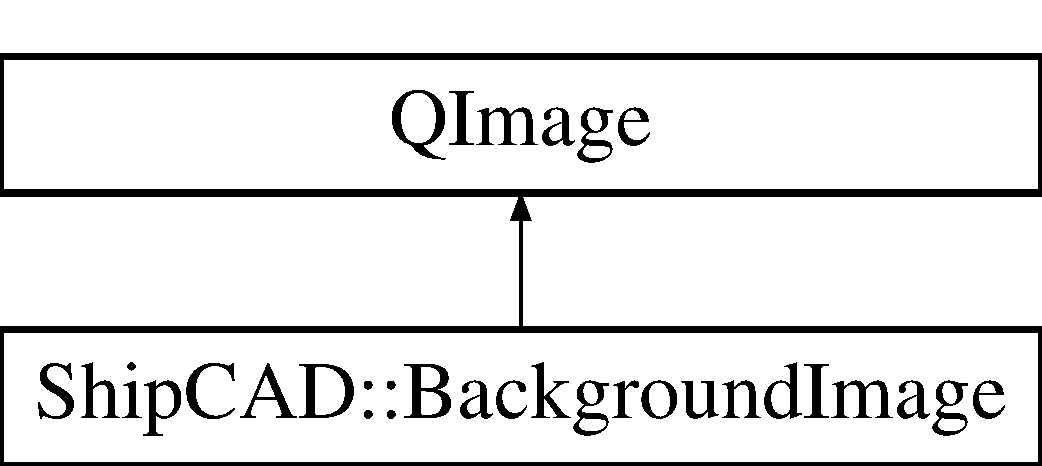
\includegraphics[height=2.000000cm]{classShipCAD_1_1BackgroundImage}
\end{center}
\end{figure}
\subsection*{Public Member Functions}
\begin{DoxyCompactItemize}
\item 
\hyperlink{classShipCAD_1_1BackgroundImage_ab37b2469c0bc2558b5eb27b42c5e30eb}{Background\-Image} (Ship\-C\-A\-D $\ast$owner)
\item 
\hyperlink{classShipCAD_1_1BackgroundImage_a77cbf94a033f736a6c7366cf1e956573}{$\sim$\-Background\-Image} ()
\item 
void \hyperlink{classShipCAD_1_1BackgroundImage_ae3b395941e8580f3921b0f9a40be71d8}{load\-Binary} (File\-Buf \&source)
\item 
void \hyperlink{classShipCAD_1_1BackgroundImage_ad5069ad93b2885d264620d36327956e9}{save\-Binary} (File\-Buf \&dest)
\item 
void \hyperlink{classShipCAD_1_1BackgroundImage_a856b8b55eafdb018792411f2edca81ef}{update\-Data} (\hyperlink{classShipCAD_1_1Viewport}{Viewport} \&vp)
\item 
void \hyperlink{classShipCAD_1_1BackgroundImage_ae64647d7f69166b1af28920953f6bfc4}{update\-Views} ()
\end{DoxyCompactItemize}


\subsection{Detailed Description}


Definition at line 45 of file backgroundimage.\-h.



\subsection{Constructor \& Destructor Documentation}
\hypertarget{classShipCAD_1_1BackgroundImage_ab37b2469c0bc2558b5eb27b42c5e30eb}{\index{Ship\-C\-A\-D\-::\-Background\-Image@{Ship\-C\-A\-D\-::\-Background\-Image}!Background\-Image@{Background\-Image}}
\index{Background\-Image@{Background\-Image}!ShipCAD::BackgroundImage@{Ship\-C\-A\-D\-::\-Background\-Image}}
\subsubsection[{Background\-Image}]{\setlength{\rightskip}{0pt plus 5cm}Ship\-C\-A\-D\-::\-Background\-Image\-::\-Background\-Image (
\begin{DoxyParamCaption}
\item[{Ship\-C\-A\-D $\ast$}]{owner}
\end{DoxyParamCaption}
)\hspace{0.3cm}{\ttfamily [explicit]}}}\label{classShipCAD_1_1BackgroundImage_ab37b2469c0bc2558b5eb27b42c5e30eb}
\hypertarget{classShipCAD_1_1BackgroundImage_a77cbf94a033f736a6c7366cf1e956573}{\index{Ship\-C\-A\-D\-::\-Background\-Image@{Ship\-C\-A\-D\-::\-Background\-Image}!$\sim$\-Background\-Image@{$\sim$\-Background\-Image}}
\index{$\sim$\-Background\-Image@{$\sim$\-Background\-Image}!ShipCAD::BackgroundImage@{Ship\-C\-A\-D\-::\-Background\-Image}}
\subsubsection[{$\sim$\-Background\-Image}]{\setlength{\rightskip}{0pt plus 5cm}Ship\-C\-A\-D\-::\-Background\-Image\-::$\sim$\-Background\-Image (
\begin{DoxyParamCaption}
{}
\end{DoxyParamCaption}
)}}\label{classShipCAD_1_1BackgroundImage_a77cbf94a033f736a6c7366cf1e956573}


\subsection{Member Function Documentation}
\hypertarget{classShipCAD_1_1BackgroundImage_ae3b395941e8580f3921b0f9a40be71d8}{\index{Ship\-C\-A\-D\-::\-Background\-Image@{Ship\-C\-A\-D\-::\-Background\-Image}!load\-Binary@{load\-Binary}}
\index{load\-Binary@{load\-Binary}!ShipCAD::BackgroundImage@{Ship\-C\-A\-D\-::\-Background\-Image}}
\subsubsection[{load\-Binary}]{\setlength{\rightskip}{0pt plus 5cm}void Ship\-C\-A\-D\-::\-Background\-Image\-::load\-Binary (
\begin{DoxyParamCaption}
\item[{File\-Buf \&}]{source}
\end{DoxyParamCaption}
)}}\label{classShipCAD_1_1BackgroundImage_ae3b395941e8580f3921b0f9a40be71d8}
\hypertarget{classShipCAD_1_1BackgroundImage_ad5069ad93b2885d264620d36327956e9}{\index{Ship\-C\-A\-D\-::\-Background\-Image@{Ship\-C\-A\-D\-::\-Background\-Image}!save\-Binary@{save\-Binary}}
\index{save\-Binary@{save\-Binary}!ShipCAD::BackgroundImage@{Ship\-C\-A\-D\-::\-Background\-Image}}
\subsubsection[{save\-Binary}]{\setlength{\rightskip}{0pt plus 5cm}void Ship\-C\-A\-D\-::\-Background\-Image\-::save\-Binary (
\begin{DoxyParamCaption}
\item[{File\-Buf \&}]{dest}
\end{DoxyParamCaption}
)}}\label{classShipCAD_1_1BackgroundImage_ad5069ad93b2885d264620d36327956e9}
\hypertarget{classShipCAD_1_1BackgroundImage_a856b8b55eafdb018792411f2edca81ef}{\index{Ship\-C\-A\-D\-::\-Background\-Image@{Ship\-C\-A\-D\-::\-Background\-Image}!update\-Data@{update\-Data}}
\index{update\-Data@{update\-Data}!ShipCAD::BackgroundImage@{Ship\-C\-A\-D\-::\-Background\-Image}}
\subsubsection[{update\-Data}]{\setlength{\rightskip}{0pt plus 5cm}void Ship\-C\-A\-D\-::\-Background\-Image\-::update\-Data (
\begin{DoxyParamCaption}
\item[{{\bf Viewport} \&}]{vp}
\end{DoxyParamCaption}
)}}\label{classShipCAD_1_1BackgroundImage_a856b8b55eafdb018792411f2edca81ef}
\hypertarget{classShipCAD_1_1BackgroundImage_ae64647d7f69166b1af28920953f6bfc4}{\index{Ship\-C\-A\-D\-::\-Background\-Image@{Ship\-C\-A\-D\-::\-Background\-Image}!update\-Views@{update\-Views}}
\index{update\-Views@{update\-Views}!ShipCAD::BackgroundImage@{Ship\-C\-A\-D\-::\-Background\-Image}}
\subsubsection[{update\-Views}]{\setlength{\rightskip}{0pt plus 5cm}void Ship\-C\-A\-D\-::\-Background\-Image\-::update\-Views (
\begin{DoxyParamCaption}
{}
\end{DoxyParamCaption}
)}}\label{classShipCAD_1_1BackgroundImage_ae64647d7f69166b1af28920953f6bfc4}


The documentation for this class was generated from the following file\-:\begin{DoxyCompactItemize}
\item 
Ship\-C\-A\-Dlib/\hyperlink{backgroundimage_8h}{backgroundimage.\-h}\end{DoxyCompactItemize}

\hypertarget{structCalculateSplineArea}{\section{Calculate\-Spline\-Area Struct Reference}
\label{structCalculateSplineArea}\index{Calculate\-Spline\-Area@{Calculate\-Spline\-Area}}
}
\subsection*{Public Member Functions}
\begin{DoxyCompactItemize}
\item 
\hyperlink{structCalculateSplineArea_aee1b91c5b5c4e58b697aa65984864e48}{Calculate\-Spline\-Area} (float $\ast$area, Q\-Vector3\-D $\ast$cog, Q\-Vector2\-D $\ast$mom\-\_\-inertia, \hyperlink{namespaceShipCAD_aa56834b730aafdf2786ddc9a60a046fd}{intersection\-\_\-type\-\_\-t} ty, const \hyperlink{classShipCAD_1_1Plane}{Plane} \&pln)
\item 
Q\-Vector2\-D \hyperlink{structCalculateSplineArea_aa1d72cbd764c437d829a04a7c4c14d9b}{Project\-To2\-D} (Q\-Vector3\-D \&p)
\item 
void \hyperlink{structCalculateSplineArea_a55da994c2b32cad71e5c8c8f21b09ce0}{operator()} (\hyperlink{classShipCAD_1_1Spline}{Spline} $\ast$spline)
\end{DoxyCompactItemize}
\subsection*{Public Attributes}
\begin{DoxyCompactItemize}
\item 
float $\ast$ \hyperlink{structCalculateSplineArea_a2b059a1a694d22a63c94bde86a8ecd6b}{\-\_\-area}
\item 
Q\-Vector3\-D $\ast$ \hyperlink{structCalculateSplineArea_abe01c8bb84cfb1900fa06e9e16fcc575}{\-\_\-cog}
\item 
Q\-Vector2\-D $\ast$ \hyperlink{structCalculateSplineArea_a5d4eebaf188d12a2f30ed7f28bf3d57f}{\-\_\-moi}
\item 
\hyperlink{namespaceShipCAD_aa56834b730aafdf2786ddc9a60a046fd}{intersection\-\_\-type\-\_\-t} \hyperlink{structCalculateSplineArea_aae716b66f114f0217e68efc79ca9cc91}{\-\_\-intersection\-\_\-type}
\item 
\hyperlink{classShipCAD_1_1Plane}{Plane} \hyperlink{structCalculateSplineArea_ab6c7f0e103a21db017e7330a31e9f984}{\-\_\-plane}
\end{DoxyCompactItemize}


\subsection{Detailed Description}


Definition at line 144 of file intersection.\-cpp.



\subsection{Constructor \& Destructor Documentation}
\hypertarget{structCalculateSplineArea_aee1b91c5b5c4e58b697aa65984864e48}{\index{Calculate\-Spline\-Area@{Calculate\-Spline\-Area}!Calculate\-Spline\-Area@{Calculate\-Spline\-Area}}
\index{Calculate\-Spline\-Area@{Calculate\-Spline\-Area}!CalculateSplineArea@{Calculate\-Spline\-Area}}
\subsubsection[{Calculate\-Spline\-Area}]{\setlength{\rightskip}{0pt plus 5cm}Calculate\-Spline\-Area\-::\-Calculate\-Spline\-Area (
\begin{DoxyParamCaption}
\item[{float $\ast$}]{area, }
\item[{Q\-Vector3\-D $\ast$}]{cog, }
\item[{Q\-Vector2\-D $\ast$}]{mom\-\_\-inertia, }
\item[{{\bf intersection\-\_\-type\-\_\-t}}]{ty, }
\item[{const {\bf Plane} \&}]{pln}
\end{DoxyParamCaption}
)\hspace{0.3cm}{\ttfamily [inline]}}}\label{structCalculateSplineArea_aee1b91c5b5c4e58b697aa65984864e48}


Definition at line 151 of file intersection.\-cpp.



\subsection{Member Function Documentation}
\hypertarget{structCalculateSplineArea_a55da994c2b32cad71e5c8c8f21b09ce0}{\index{Calculate\-Spline\-Area@{Calculate\-Spline\-Area}!operator()@{operator()}}
\index{operator()@{operator()}!CalculateSplineArea@{Calculate\-Spline\-Area}}
\subsubsection[{operator()}]{\setlength{\rightskip}{0pt plus 5cm}void Calculate\-Spline\-Area\-::operator() (
\begin{DoxyParamCaption}
\item[{{\bf Spline} $\ast$}]{spline}
\end{DoxyParamCaption}
)\hspace{0.3cm}{\ttfamily [inline]}}}\label{structCalculateSplineArea_a55da994c2b32cad71e5c8c8f21b09ce0}


Definition at line 173 of file intersection.\-cpp.

\hypertarget{structCalculateSplineArea_aa1d72cbd764c437d829a04a7c4c14d9b}{\index{Calculate\-Spline\-Area@{Calculate\-Spline\-Area}!Project\-To2\-D@{Project\-To2\-D}}
\index{Project\-To2\-D@{Project\-To2\-D}!CalculateSplineArea@{Calculate\-Spline\-Area}}
\subsubsection[{Project\-To2\-D}]{\setlength{\rightskip}{0pt plus 5cm}Q\-Vector2\-D Calculate\-Spline\-Area\-::\-Project\-To2\-D (
\begin{DoxyParamCaption}
\item[{Q\-Vector3\-D \&}]{p}
\end{DoxyParamCaption}
)\hspace{0.3cm}{\ttfamily [inline]}}}\label{structCalculateSplineArea_aa1d72cbd764c437d829a04a7c4c14d9b}


Definition at line 154 of file intersection.\-cpp.



\subsection{Member Data Documentation}
\hypertarget{structCalculateSplineArea_a2b059a1a694d22a63c94bde86a8ecd6b}{\index{Calculate\-Spline\-Area@{Calculate\-Spline\-Area}!\-\_\-area@{\-\_\-area}}
\index{\-\_\-area@{\-\_\-area}!CalculateSplineArea@{Calculate\-Spline\-Area}}
\subsubsection[{\-\_\-area}]{\setlength{\rightskip}{0pt plus 5cm}float$\ast$ Calculate\-Spline\-Area\-::\-\_\-area}}\label{structCalculateSplineArea_a2b059a1a694d22a63c94bde86a8ecd6b}


Definition at line 146 of file intersection.\-cpp.

\hypertarget{structCalculateSplineArea_abe01c8bb84cfb1900fa06e9e16fcc575}{\index{Calculate\-Spline\-Area@{Calculate\-Spline\-Area}!\-\_\-cog@{\-\_\-cog}}
\index{\-\_\-cog@{\-\_\-cog}!CalculateSplineArea@{Calculate\-Spline\-Area}}
\subsubsection[{\-\_\-cog}]{\setlength{\rightskip}{0pt plus 5cm}Q\-Vector3\-D$\ast$ Calculate\-Spline\-Area\-::\-\_\-cog}}\label{structCalculateSplineArea_abe01c8bb84cfb1900fa06e9e16fcc575}


Definition at line 147 of file intersection.\-cpp.

\hypertarget{structCalculateSplineArea_aae716b66f114f0217e68efc79ca9cc91}{\index{Calculate\-Spline\-Area@{Calculate\-Spline\-Area}!\-\_\-intersection\-\_\-type@{\-\_\-intersection\-\_\-type}}
\index{\-\_\-intersection\-\_\-type@{\-\_\-intersection\-\_\-type}!CalculateSplineArea@{Calculate\-Spline\-Area}}
\subsubsection[{\-\_\-intersection\-\_\-type}]{\setlength{\rightskip}{0pt plus 5cm}{\bf intersection\-\_\-type\-\_\-t} Calculate\-Spline\-Area\-::\-\_\-intersection\-\_\-type}}\label{structCalculateSplineArea_aae716b66f114f0217e68efc79ca9cc91}


Definition at line 149 of file intersection.\-cpp.

\hypertarget{structCalculateSplineArea_a5d4eebaf188d12a2f30ed7f28bf3d57f}{\index{Calculate\-Spline\-Area@{Calculate\-Spline\-Area}!\-\_\-moi@{\-\_\-moi}}
\index{\-\_\-moi@{\-\_\-moi}!CalculateSplineArea@{Calculate\-Spline\-Area}}
\subsubsection[{\-\_\-moi}]{\setlength{\rightskip}{0pt plus 5cm}Q\-Vector2\-D$\ast$ Calculate\-Spline\-Area\-::\-\_\-moi}}\label{structCalculateSplineArea_a5d4eebaf188d12a2f30ed7f28bf3d57f}


Definition at line 148 of file intersection.\-cpp.

\hypertarget{structCalculateSplineArea_ab6c7f0e103a21db017e7330a31e9f984}{\index{Calculate\-Spline\-Area@{Calculate\-Spline\-Area}!\-\_\-plane@{\-\_\-plane}}
\index{\-\_\-plane@{\-\_\-plane}!CalculateSplineArea@{Calculate\-Spline\-Area}}
\subsubsection[{\-\_\-plane}]{\setlength{\rightskip}{0pt plus 5cm}{\bf Plane} Calculate\-Spline\-Area\-::\-\_\-plane}}\label{structCalculateSplineArea_ab6c7f0e103a21db017e7330a31e9f984}


Definition at line 150 of file intersection.\-cpp.



The documentation for this struct was generated from the following file\-:\begin{DoxyCompactItemize}
\item 
Ship\-C\-A\-Dlib/\hyperlink{intersection_8cpp}{intersection.\-cpp}\end{DoxyCompactItemize}

\hypertarget{unionconvert__type__t}{\section{convert\-\_\-type\-\_\-t Union Reference}
\label{unionconvert__type__t}\index{convert\-\_\-type\-\_\-t@{convert\-\_\-type\-\_\-t}}
}
\subsection*{Public Attributes}
\begin{DoxyCompactItemize}
\item 
unsigned char \hyperlink{unionconvert__type__t_a6f76840d6875059c2655f53246c5a5a1}{d} \mbox{[}8\mbox{]}
\item 
int \hyperlink{unionconvert__type__t_a9eef931dacbc2c9fe0b67edc5e053624}{ival}
\item 
size\-\_\-t \hyperlink{unionconvert__type__t_ab2a3ae21cfb1610cc473234ce3e7661e}{uval}
\item 
float \hyperlink{unionconvert__type__t_aa56281b3a5e206689c30ce623aa6dc0b}{fval}
\end{DoxyCompactItemize}


\subsection{Detailed Description}


Definition at line 41 of file filebuffer.\-cpp.



\subsection{Member Data Documentation}
\hypertarget{unionconvert__type__t_a6f76840d6875059c2655f53246c5a5a1}{\index{convert\-\_\-type\-\_\-t@{convert\-\_\-type\-\_\-t}!d@{d}}
\index{d@{d}!convert_type_t@{convert\-\_\-type\-\_\-t}}
\subsubsection[{d}]{\setlength{\rightskip}{0pt plus 5cm}unsigned char convert\-\_\-type\-\_\-t\-::d\mbox{[}8\mbox{]}}}\label{unionconvert__type__t_a6f76840d6875059c2655f53246c5a5a1}


Definition at line 42 of file filebuffer.\-cpp.

\hypertarget{unionconvert__type__t_aa56281b3a5e206689c30ce623aa6dc0b}{\index{convert\-\_\-type\-\_\-t@{convert\-\_\-type\-\_\-t}!fval@{fval}}
\index{fval@{fval}!convert_type_t@{convert\-\_\-type\-\_\-t}}
\subsubsection[{fval}]{\setlength{\rightskip}{0pt plus 5cm}float convert\-\_\-type\-\_\-t\-::fval}}\label{unionconvert__type__t_aa56281b3a5e206689c30ce623aa6dc0b}


Definition at line 45 of file filebuffer.\-cpp.

\hypertarget{unionconvert__type__t_a9eef931dacbc2c9fe0b67edc5e053624}{\index{convert\-\_\-type\-\_\-t@{convert\-\_\-type\-\_\-t}!ival@{ival}}
\index{ival@{ival}!convert_type_t@{convert\-\_\-type\-\_\-t}}
\subsubsection[{ival}]{\setlength{\rightskip}{0pt plus 5cm}int convert\-\_\-type\-\_\-t\-::ival}}\label{unionconvert__type__t_a9eef931dacbc2c9fe0b67edc5e053624}


Definition at line 43 of file filebuffer.\-cpp.

\hypertarget{unionconvert__type__t_ab2a3ae21cfb1610cc473234ce3e7661e}{\index{convert\-\_\-type\-\_\-t@{convert\-\_\-type\-\_\-t}!uval@{uval}}
\index{uval@{uval}!convert_type_t@{convert\-\_\-type\-\_\-t}}
\subsubsection[{uval}]{\setlength{\rightskip}{0pt plus 5cm}size\-\_\-t convert\-\_\-type\-\_\-t\-::uval}}\label{unionconvert__type__t_ab2a3ae21cfb1610cc473234ce3e7661e}


Definition at line 44 of file filebuffer.\-cpp.



The documentation for this union was generated from the following file\-:\begin{DoxyCompactItemize}
\item 
Ship\-C\-A\-Dlib/\hyperlink{filebuffer_8cpp}{filebuffer.\-cpp}\end{DoxyCompactItemize}

\hypertarget{structShipCAD_1_1CrosscurvesData}{\section{Ship\-C\-A\-D\-:\-:Crosscurves\-Data Struct Reference}
\label{structShipCAD_1_1CrosscurvesData}\index{Ship\-C\-A\-D\-::\-Crosscurves\-Data@{Ship\-C\-A\-D\-::\-Crosscurves\-Data}}
}


{\ttfamily \#include $<$hydrostaticcalc.\-h$>$}

\subsection*{Public Attributes}
\begin{DoxyCompactItemize}
\item 
\hyperlink{classShipCAD_1_1Plane}{Plane} \hyperlink{structShipCAD_1_1CrosscurvesData_a1ea6de1b52289e8392e8d499ae4aad04}{waterline\-\_\-plane}
\item 
float \hyperlink{structShipCAD_1_1CrosscurvesData_a759e5729cdb86d8367b139e66fecb7d3}{absolute\-\_\-draft}
\item 
float \hyperlink{structShipCAD_1_1CrosscurvesData_a9bec38a77bf87ab5feb76899e39e4f7b}{volume}
\item 
float \hyperlink{structShipCAD_1_1CrosscurvesData_a9a7baa66159e203888390eaa63caf708}{displacement}
\item 
Q\-Vector3\-D \hyperlink{structShipCAD_1_1CrosscurvesData_a0de723cd5ae0e18953fb7ad5a0f5dadf}{center\-\_\-of\-\_\-buoyancy}
\item 
float \hyperlink{structShipCAD_1_1CrosscurvesData_a55150860fed821e314e18b72f1975749}{kn\-\_\-sin\-\_\-phi}
\end{DoxyCompactItemize}


\subsection{Detailed Description}


Definition at line 84 of file hydrostaticcalc.\-h.



\subsection{Member Data Documentation}
\hypertarget{structShipCAD_1_1CrosscurvesData_a759e5729cdb86d8367b139e66fecb7d3}{\index{Ship\-C\-A\-D\-::\-Crosscurves\-Data@{Ship\-C\-A\-D\-::\-Crosscurves\-Data}!absolute\-\_\-draft@{absolute\-\_\-draft}}
\index{absolute\-\_\-draft@{absolute\-\_\-draft}!ShipCAD::CrosscurvesData@{Ship\-C\-A\-D\-::\-Crosscurves\-Data}}
\subsubsection[{absolute\-\_\-draft}]{\setlength{\rightskip}{0pt plus 5cm}float Ship\-C\-A\-D\-::\-Crosscurves\-Data\-::absolute\-\_\-draft}}\label{structShipCAD_1_1CrosscurvesData_a759e5729cdb86d8367b139e66fecb7d3}


Definition at line 87 of file hydrostaticcalc.\-h.

\hypertarget{structShipCAD_1_1CrosscurvesData_a0de723cd5ae0e18953fb7ad5a0f5dadf}{\index{Ship\-C\-A\-D\-::\-Crosscurves\-Data@{Ship\-C\-A\-D\-::\-Crosscurves\-Data}!center\-\_\-of\-\_\-buoyancy@{center\-\_\-of\-\_\-buoyancy}}
\index{center\-\_\-of\-\_\-buoyancy@{center\-\_\-of\-\_\-buoyancy}!ShipCAD::CrosscurvesData@{Ship\-C\-A\-D\-::\-Crosscurves\-Data}}
\subsubsection[{center\-\_\-of\-\_\-buoyancy}]{\setlength{\rightskip}{0pt plus 5cm}Q\-Vector3\-D Ship\-C\-A\-D\-::\-Crosscurves\-Data\-::center\-\_\-of\-\_\-buoyancy}}\label{structShipCAD_1_1CrosscurvesData_a0de723cd5ae0e18953fb7ad5a0f5dadf}


Definition at line 90 of file hydrostaticcalc.\-h.

\hypertarget{structShipCAD_1_1CrosscurvesData_a9a7baa66159e203888390eaa63caf708}{\index{Ship\-C\-A\-D\-::\-Crosscurves\-Data@{Ship\-C\-A\-D\-::\-Crosscurves\-Data}!displacement@{displacement}}
\index{displacement@{displacement}!ShipCAD::CrosscurvesData@{Ship\-C\-A\-D\-::\-Crosscurves\-Data}}
\subsubsection[{displacement}]{\setlength{\rightskip}{0pt plus 5cm}float Ship\-C\-A\-D\-::\-Crosscurves\-Data\-::displacement}}\label{structShipCAD_1_1CrosscurvesData_a9a7baa66159e203888390eaa63caf708}


Definition at line 89 of file hydrostaticcalc.\-h.

\hypertarget{structShipCAD_1_1CrosscurvesData_a55150860fed821e314e18b72f1975749}{\index{Ship\-C\-A\-D\-::\-Crosscurves\-Data@{Ship\-C\-A\-D\-::\-Crosscurves\-Data}!kn\-\_\-sin\-\_\-phi@{kn\-\_\-sin\-\_\-phi}}
\index{kn\-\_\-sin\-\_\-phi@{kn\-\_\-sin\-\_\-phi}!ShipCAD::CrosscurvesData@{Ship\-C\-A\-D\-::\-Crosscurves\-Data}}
\subsubsection[{kn\-\_\-sin\-\_\-phi}]{\setlength{\rightskip}{0pt plus 5cm}float Ship\-C\-A\-D\-::\-Crosscurves\-Data\-::kn\-\_\-sin\-\_\-phi}}\label{structShipCAD_1_1CrosscurvesData_a55150860fed821e314e18b72f1975749}


Definition at line 91 of file hydrostaticcalc.\-h.

\hypertarget{structShipCAD_1_1CrosscurvesData_a9bec38a77bf87ab5feb76899e39e4f7b}{\index{Ship\-C\-A\-D\-::\-Crosscurves\-Data@{Ship\-C\-A\-D\-::\-Crosscurves\-Data}!volume@{volume}}
\index{volume@{volume}!ShipCAD::CrosscurvesData@{Ship\-C\-A\-D\-::\-Crosscurves\-Data}}
\subsubsection[{volume}]{\setlength{\rightskip}{0pt plus 5cm}float Ship\-C\-A\-D\-::\-Crosscurves\-Data\-::volume}}\label{structShipCAD_1_1CrosscurvesData_a9bec38a77bf87ab5feb76899e39e4f7b}


Definition at line 88 of file hydrostaticcalc.\-h.

\hypertarget{structShipCAD_1_1CrosscurvesData_a1ea6de1b52289e8392e8d499ae4aad04}{\index{Ship\-C\-A\-D\-::\-Crosscurves\-Data@{Ship\-C\-A\-D\-::\-Crosscurves\-Data}!waterline\-\_\-plane@{waterline\-\_\-plane}}
\index{waterline\-\_\-plane@{waterline\-\_\-plane}!ShipCAD::CrosscurvesData@{Ship\-C\-A\-D\-::\-Crosscurves\-Data}}
\subsubsection[{waterline\-\_\-plane}]{\setlength{\rightskip}{0pt plus 5cm}{\bf Plane} Ship\-C\-A\-D\-::\-Crosscurves\-Data\-::waterline\-\_\-plane}}\label{structShipCAD_1_1CrosscurvesData_a1ea6de1b52289e8392e8d499ae4aad04}


Definition at line 86 of file hydrostaticcalc.\-h.



The documentation for this struct was generated from the following file\-:\begin{DoxyCompactItemize}
\item 
Ship\-C\-A\-Dlib/\hyperlink{hydrostaticcalc_8h}{hydrostaticcalc.\-h}\end{DoxyCompactItemize}

\hypertarget{structShipCAD_1_1DelftSeriesResistance}{\section{Ship\-C\-A\-D\-:\-:Delft\-Series\-Resistance Struct Reference}
\label{structShipCAD_1_1DelftSeriesResistance}\index{Ship\-C\-A\-D\-::\-Delft\-Series\-Resistance@{Ship\-C\-A\-D\-::\-Delft\-Series\-Resistance}}
}


{\ttfamily \#include $<$resistance.\-h$>$}

\subsection*{Public Attributes}
\begin{DoxyCompactItemize}
\item 
float \hyperlink{structShipCAD_1_1DelftSeriesResistance_a040e0d678c7dbc24c29b7da618b4094d}{start\-\_\-speed}
\item 
float \hyperlink{structShipCAD_1_1DelftSeriesResistance_abd1672b905c07093735775ff455e5a98}{end\-\_\-speed}
\item 
float \hyperlink{structShipCAD_1_1DelftSeriesResistance_a0e3ee6d984afd4ddf1cf483261904574}{step\-\_\-speed}
\item 
float \hyperlink{structShipCAD_1_1DelftSeriesResistance_a160c7b99be523bcda5301231806af6b3}{bwl}
\item 
float \hyperlink{structShipCAD_1_1DelftSeriesResistance_ae489114ad6f1d03758420f77b58de519}{cp}
\item 
float \hyperlink{structShipCAD_1_1DelftSeriesResistance_a1c98fdc7b3c1b28f6f8029af2e009992}{displacement}
\item 
float \hyperlink{structShipCAD_1_1DelftSeriesResistance_a208e360c5ca0d029f9f433a7bc2cade2}{draft}
\item 
float \hyperlink{structShipCAD_1_1DelftSeriesResistance_a4db81049e448c381019f97dc630d51af}{draft\-\_\-total}
\item 
float \hyperlink{structShipCAD_1_1DelftSeriesResistance_a986244b5c6944f01dbdae5d54b895c84}{keel\-\_\-chord\-\_\-length}
\item 
float \hyperlink{structShipCAD_1_1DelftSeriesResistance_ab1bf49519c2ed054b7699898d7f5aead}{keel\-\_\-area}
\item 
float \hyperlink{structShipCAD_1_1DelftSeriesResistance_aca93b2c11316e29b2f98a3bdcdf65bc5}{lcb}
\item 
float \hyperlink{structShipCAD_1_1DelftSeriesResistance_a7232b8ea3003087a4772a650319ec8f2}{lwl}
\item 
float \hyperlink{structShipCAD_1_1DelftSeriesResistance_a5a348a92e0ba99368c50f72c81a9b0ff}{rudder\-\_\-chord\-\_\-length}
\item 
float \hyperlink{structShipCAD_1_1DelftSeriesResistance_a9737974d43a292c58a2e24f7c78c1ffb}{rudder\-\_\-area}
\item 
float \hyperlink{structShipCAD_1_1DelftSeriesResistance_a08ff900d51b56d7e1726cb4b5a6ffa9b}{viscosity}
\item 
float \hyperlink{structShipCAD_1_1DelftSeriesResistance_a7ee0a7e2d05634beb7fb9951d80c7557}{wetted\-\_\-surface}
\item 
float \hyperlink{structShipCAD_1_1DelftSeriesResistance_af51e72b70af1ce87cf7ac641df93c541}{wl\-\_\-area}
\item 
bool \hyperlink{structShipCAD_1_1DelftSeriesResistance_a0507b03a9329185d961cd97739237d91}{estimate\-\_\-wet\-\_\-surf}
\item 
bool \hyperlink{structShipCAD_1_1DelftSeriesResistance_a8276aa04952e727f1a310f10ceb72414}{extract}
\item 
quint8 \hyperlink{structShipCAD_1_1DelftSeriesResistance_acd08ff15cfab748bf4f54aa65b927950}{padding} \mbox{[}2\mbox{]}
\end{DoxyCompactItemize}


\subsection{Detailed Description}


Definition at line 38 of file resistance.\-h.



\subsection{Member Data Documentation}
\hypertarget{structShipCAD_1_1DelftSeriesResistance_a160c7b99be523bcda5301231806af6b3}{\index{Ship\-C\-A\-D\-::\-Delft\-Series\-Resistance@{Ship\-C\-A\-D\-::\-Delft\-Series\-Resistance}!bwl@{bwl}}
\index{bwl@{bwl}!ShipCAD::DelftSeriesResistance@{Ship\-C\-A\-D\-::\-Delft\-Series\-Resistance}}
\subsubsection[{bwl}]{\setlength{\rightskip}{0pt plus 5cm}float Ship\-C\-A\-D\-::\-Delft\-Series\-Resistance\-::bwl}}\label{structShipCAD_1_1DelftSeriesResistance_a160c7b99be523bcda5301231806af6b3}


Definition at line 43 of file resistance.\-h.

\hypertarget{structShipCAD_1_1DelftSeriesResistance_ae489114ad6f1d03758420f77b58de519}{\index{Ship\-C\-A\-D\-::\-Delft\-Series\-Resistance@{Ship\-C\-A\-D\-::\-Delft\-Series\-Resistance}!cp@{cp}}
\index{cp@{cp}!ShipCAD::DelftSeriesResistance@{Ship\-C\-A\-D\-::\-Delft\-Series\-Resistance}}
\subsubsection[{cp}]{\setlength{\rightskip}{0pt plus 5cm}float Ship\-C\-A\-D\-::\-Delft\-Series\-Resistance\-::cp}}\label{structShipCAD_1_1DelftSeriesResistance_ae489114ad6f1d03758420f77b58de519}


Definition at line 44 of file resistance.\-h.

\hypertarget{structShipCAD_1_1DelftSeriesResistance_a1c98fdc7b3c1b28f6f8029af2e009992}{\index{Ship\-C\-A\-D\-::\-Delft\-Series\-Resistance@{Ship\-C\-A\-D\-::\-Delft\-Series\-Resistance}!displacement@{displacement}}
\index{displacement@{displacement}!ShipCAD::DelftSeriesResistance@{Ship\-C\-A\-D\-::\-Delft\-Series\-Resistance}}
\subsubsection[{displacement}]{\setlength{\rightskip}{0pt plus 5cm}float Ship\-C\-A\-D\-::\-Delft\-Series\-Resistance\-::displacement}}\label{structShipCAD_1_1DelftSeriesResistance_a1c98fdc7b3c1b28f6f8029af2e009992}


Definition at line 45 of file resistance.\-h.

\hypertarget{structShipCAD_1_1DelftSeriesResistance_a208e360c5ca0d029f9f433a7bc2cade2}{\index{Ship\-C\-A\-D\-::\-Delft\-Series\-Resistance@{Ship\-C\-A\-D\-::\-Delft\-Series\-Resistance}!draft@{draft}}
\index{draft@{draft}!ShipCAD::DelftSeriesResistance@{Ship\-C\-A\-D\-::\-Delft\-Series\-Resistance}}
\subsubsection[{draft}]{\setlength{\rightskip}{0pt plus 5cm}float Ship\-C\-A\-D\-::\-Delft\-Series\-Resistance\-::draft}}\label{structShipCAD_1_1DelftSeriesResistance_a208e360c5ca0d029f9f433a7bc2cade2}


Definition at line 46 of file resistance.\-h.

\hypertarget{structShipCAD_1_1DelftSeriesResistance_a4db81049e448c381019f97dc630d51af}{\index{Ship\-C\-A\-D\-::\-Delft\-Series\-Resistance@{Ship\-C\-A\-D\-::\-Delft\-Series\-Resistance}!draft\-\_\-total@{draft\-\_\-total}}
\index{draft\-\_\-total@{draft\-\_\-total}!ShipCAD::DelftSeriesResistance@{Ship\-C\-A\-D\-::\-Delft\-Series\-Resistance}}
\subsubsection[{draft\-\_\-total}]{\setlength{\rightskip}{0pt plus 5cm}float Ship\-C\-A\-D\-::\-Delft\-Series\-Resistance\-::draft\-\_\-total}}\label{structShipCAD_1_1DelftSeriesResistance_a4db81049e448c381019f97dc630d51af}


Definition at line 47 of file resistance.\-h.

\hypertarget{structShipCAD_1_1DelftSeriesResistance_abd1672b905c07093735775ff455e5a98}{\index{Ship\-C\-A\-D\-::\-Delft\-Series\-Resistance@{Ship\-C\-A\-D\-::\-Delft\-Series\-Resistance}!end\-\_\-speed@{end\-\_\-speed}}
\index{end\-\_\-speed@{end\-\_\-speed}!ShipCAD::DelftSeriesResistance@{Ship\-C\-A\-D\-::\-Delft\-Series\-Resistance}}
\subsubsection[{end\-\_\-speed}]{\setlength{\rightskip}{0pt plus 5cm}float Ship\-C\-A\-D\-::\-Delft\-Series\-Resistance\-::end\-\_\-speed}}\label{structShipCAD_1_1DelftSeriesResistance_abd1672b905c07093735775ff455e5a98}


Definition at line 41 of file resistance.\-h.

\hypertarget{structShipCAD_1_1DelftSeriesResistance_a0507b03a9329185d961cd97739237d91}{\index{Ship\-C\-A\-D\-::\-Delft\-Series\-Resistance@{Ship\-C\-A\-D\-::\-Delft\-Series\-Resistance}!estimate\-\_\-wet\-\_\-surf@{estimate\-\_\-wet\-\_\-surf}}
\index{estimate\-\_\-wet\-\_\-surf@{estimate\-\_\-wet\-\_\-surf}!ShipCAD::DelftSeriesResistance@{Ship\-C\-A\-D\-::\-Delft\-Series\-Resistance}}
\subsubsection[{estimate\-\_\-wet\-\_\-surf}]{\setlength{\rightskip}{0pt plus 5cm}bool Ship\-C\-A\-D\-::\-Delft\-Series\-Resistance\-::estimate\-\_\-wet\-\_\-surf}}\label{structShipCAD_1_1DelftSeriesResistance_a0507b03a9329185d961cd97739237d91}


Definition at line 57 of file resistance.\-h.

\hypertarget{structShipCAD_1_1DelftSeriesResistance_a8276aa04952e727f1a310f10ceb72414}{\index{Ship\-C\-A\-D\-::\-Delft\-Series\-Resistance@{Ship\-C\-A\-D\-::\-Delft\-Series\-Resistance}!extract@{extract}}
\index{extract@{extract}!ShipCAD::DelftSeriesResistance@{Ship\-C\-A\-D\-::\-Delft\-Series\-Resistance}}
\subsubsection[{extract}]{\setlength{\rightskip}{0pt plus 5cm}bool Ship\-C\-A\-D\-::\-Delft\-Series\-Resistance\-::extract}}\label{structShipCAD_1_1DelftSeriesResistance_a8276aa04952e727f1a310f10ceb72414}


Definition at line 58 of file resistance.\-h.

\hypertarget{structShipCAD_1_1DelftSeriesResistance_ab1bf49519c2ed054b7699898d7f5aead}{\index{Ship\-C\-A\-D\-::\-Delft\-Series\-Resistance@{Ship\-C\-A\-D\-::\-Delft\-Series\-Resistance}!keel\-\_\-area@{keel\-\_\-area}}
\index{keel\-\_\-area@{keel\-\_\-area}!ShipCAD::DelftSeriesResistance@{Ship\-C\-A\-D\-::\-Delft\-Series\-Resistance}}
\subsubsection[{keel\-\_\-area}]{\setlength{\rightskip}{0pt plus 5cm}float Ship\-C\-A\-D\-::\-Delft\-Series\-Resistance\-::keel\-\_\-area}}\label{structShipCAD_1_1DelftSeriesResistance_ab1bf49519c2ed054b7699898d7f5aead}


Definition at line 49 of file resistance.\-h.

\hypertarget{structShipCAD_1_1DelftSeriesResistance_a986244b5c6944f01dbdae5d54b895c84}{\index{Ship\-C\-A\-D\-::\-Delft\-Series\-Resistance@{Ship\-C\-A\-D\-::\-Delft\-Series\-Resistance}!keel\-\_\-chord\-\_\-length@{keel\-\_\-chord\-\_\-length}}
\index{keel\-\_\-chord\-\_\-length@{keel\-\_\-chord\-\_\-length}!ShipCAD::DelftSeriesResistance@{Ship\-C\-A\-D\-::\-Delft\-Series\-Resistance}}
\subsubsection[{keel\-\_\-chord\-\_\-length}]{\setlength{\rightskip}{0pt plus 5cm}float Ship\-C\-A\-D\-::\-Delft\-Series\-Resistance\-::keel\-\_\-chord\-\_\-length}}\label{structShipCAD_1_1DelftSeriesResistance_a986244b5c6944f01dbdae5d54b895c84}


Definition at line 48 of file resistance.\-h.

\hypertarget{structShipCAD_1_1DelftSeriesResistance_aca93b2c11316e29b2f98a3bdcdf65bc5}{\index{Ship\-C\-A\-D\-::\-Delft\-Series\-Resistance@{Ship\-C\-A\-D\-::\-Delft\-Series\-Resistance}!lcb@{lcb}}
\index{lcb@{lcb}!ShipCAD::DelftSeriesResistance@{Ship\-C\-A\-D\-::\-Delft\-Series\-Resistance}}
\subsubsection[{lcb}]{\setlength{\rightskip}{0pt plus 5cm}float Ship\-C\-A\-D\-::\-Delft\-Series\-Resistance\-::lcb}}\label{structShipCAD_1_1DelftSeriesResistance_aca93b2c11316e29b2f98a3bdcdf65bc5}


Definition at line 50 of file resistance.\-h.

\hypertarget{structShipCAD_1_1DelftSeriesResistance_a7232b8ea3003087a4772a650319ec8f2}{\index{Ship\-C\-A\-D\-::\-Delft\-Series\-Resistance@{Ship\-C\-A\-D\-::\-Delft\-Series\-Resistance}!lwl@{lwl}}
\index{lwl@{lwl}!ShipCAD::DelftSeriesResistance@{Ship\-C\-A\-D\-::\-Delft\-Series\-Resistance}}
\subsubsection[{lwl}]{\setlength{\rightskip}{0pt plus 5cm}float Ship\-C\-A\-D\-::\-Delft\-Series\-Resistance\-::lwl}}\label{structShipCAD_1_1DelftSeriesResistance_a7232b8ea3003087a4772a650319ec8f2}


Definition at line 51 of file resistance.\-h.

\hypertarget{structShipCAD_1_1DelftSeriesResistance_acd08ff15cfab748bf4f54aa65b927950}{\index{Ship\-C\-A\-D\-::\-Delft\-Series\-Resistance@{Ship\-C\-A\-D\-::\-Delft\-Series\-Resistance}!padding@{padding}}
\index{padding@{padding}!ShipCAD::DelftSeriesResistance@{Ship\-C\-A\-D\-::\-Delft\-Series\-Resistance}}
\subsubsection[{padding}]{\setlength{\rightskip}{0pt plus 5cm}quint8 Ship\-C\-A\-D\-::\-Delft\-Series\-Resistance\-::padding\mbox{[}2\mbox{]}}}\label{structShipCAD_1_1DelftSeriesResistance_acd08ff15cfab748bf4f54aa65b927950}


Definition at line 63 of file resistance.\-h.

\hypertarget{structShipCAD_1_1DelftSeriesResistance_a9737974d43a292c58a2e24f7c78c1ffb}{\index{Ship\-C\-A\-D\-::\-Delft\-Series\-Resistance@{Ship\-C\-A\-D\-::\-Delft\-Series\-Resistance}!rudder\-\_\-area@{rudder\-\_\-area}}
\index{rudder\-\_\-area@{rudder\-\_\-area}!ShipCAD::DelftSeriesResistance@{Ship\-C\-A\-D\-::\-Delft\-Series\-Resistance}}
\subsubsection[{rudder\-\_\-area}]{\setlength{\rightskip}{0pt plus 5cm}float Ship\-C\-A\-D\-::\-Delft\-Series\-Resistance\-::rudder\-\_\-area}}\label{structShipCAD_1_1DelftSeriesResistance_a9737974d43a292c58a2e24f7c78c1ffb}


Definition at line 53 of file resistance.\-h.

\hypertarget{structShipCAD_1_1DelftSeriesResistance_a5a348a92e0ba99368c50f72c81a9b0ff}{\index{Ship\-C\-A\-D\-::\-Delft\-Series\-Resistance@{Ship\-C\-A\-D\-::\-Delft\-Series\-Resistance}!rudder\-\_\-chord\-\_\-length@{rudder\-\_\-chord\-\_\-length}}
\index{rudder\-\_\-chord\-\_\-length@{rudder\-\_\-chord\-\_\-length}!ShipCAD::DelftSeriesResistance@{Ship\-C\-A\-D\-::\-Delft\-Series\-Resistance}}
\subsubsection[{rudder\-\_\-chord\-\_\-length}]{\setlength{\rightskip}{0pt plus 5cm}float Ship\-C\-A\-D\-::\-Delft\-Series\-Resistance\-::rudder\-\_\-chord\-\_\-length}}\label{structShipCAD_1_1DelftSeriesResistance_a5a348a92e0ba99368c50f72c81a9b0ff}


Definition at line 52 of file resistance.\-h.

\hypertarget{structShipCAD_1_1DelftSeriesResistance_a040e0d678c7dbc24c29b7da618b4094d}{\index{Ship\-C\-A\-D\-::\-Delft\-Series\-Resistance@{Ship\-C\-A\-D\-::\-Delft\-Series\-Resistance}!start\-\_\-speed@{start\-\_\-speed}}
\index{start\-\_\-speed@{start\-\_\-speed}!ShipCAD::DelftSeriesResistance@{Ship\-C\-A\-D\-::\-Delft\-Series\-Resistance}}
\subsubsection[{start\-\_\-speed}]{\setlength{\rightskip}{0pt plus 5cm}float Ship\-C\-A\-D\-::\-Delft\-Series\-Resistance\-::start\-\_\-speed}}\label{structShipCAD_1_1DelftSeriesResistance_a040e0d678c7dbc24c29b7da618b4094d}


Definition at line 40 of file resistance.\-h.

\hypertarget{structShipCAD_1_1DelftSeriesResistance_a0e3ee6d984afd4ddf1cf483261904574}{\index{Ship\-C\-A\-D\-::\-Delft\-Series\-Resistance@{Ship\-C\-A\-D\-::\-Delft\-Series\-Resistance}!step\-\_\-speed@{step\-\_\-speed}}
\index{step\-\_\-speed@{step\-\_\-speed}!ShipCAD::DelftSeriesResistance@{Ship\-C\-A\-D\-::\-Delft\-Series\-Resistance}}
\subsubsection[{step\-\_\-speed}]{\setlength{\rightskip}{0pt plus 5cm}float Ship\-C\-A\-D\-::\-Delft\-Series\-Resistance\-::step\-\_\-speed}}\label{structShipCAD_1_1DelftSeriesResistance_a0e3ee6d984afd4ddf1cf483261904574}


Definition at line 42 of file resistance.\-h.

\hypertarget{structShipCAD_1_1DelftSeriesResistance_a08ff900d51b56d7e1726cb4b5a6ffa9b}{\index{Ship\-C\-A\-D\-::\-Delft\-Series\-Resistance@{Ship\-C\-A\-D\-::\-Delft\-Series\-Resistance}!viscosity@{viscosity}}
\index{viscosity@{viscosity}!ShipCAD::DelftSeriesResistance@{Ship\-C\-A\-D\-::\-Delft\-Series\-Resistance}}
\subsubsection[{viscosity}]{\setlength{\rightskip}{0pt plus 5cm}float Ship\-C\-A\-D\-::\-Delft\-Series\-Resistance\-::viscosity}}\label{structShipCAD_1_1DelftSeriesResistance_a08ff900d51b56d7e1726cb4b5a6ffa9b}


Definition at line 54 of file resistance.\-h.

\hypertarget{structShipCAD_1_1DelftSeriesResistance_a7ee0a7e2d05634beb7fb9951d80c7557}{\index{Ship\-C\-A\-D\-::\-Delft\-Series\-Resistance@{Ship\-C\-A\-D\-::\-Delft\-Series\-Resistance}!wetted\-\_\-surface@{wetted\-\_\-surface}}
\index{wetted\-\_\-surface@{wetted\-\_\-surface}!ShipCAD::DelftSeriesResistance@{Ship\-C\-A\-D\-::\-Delft\-Series\-Resistance}}
\subsubsection[{wetted\-\_\-surface}]{\setlength{\rightskip}{0pt plus 5cm}float Ship\-C\-A\-D\-::\-Delft\-Series\-Resistance\-::wetted\-\_\-surface}}\label{structShipCAD_1_1DelftSeriesResistance_a7ee0a7e2d05634beb7fb9951d80c7557}


Definition at line 55 of file resistance.\-h.

\hypertarget{structShipCAD_1_1DelftSeriesResistance_af51e72b70af1ce87cf7ac641df93c541}{\index{Ship\-C\-A\-D\-::\-Delft\-Series\-Resistance@{Ship\-C\-A\-D\-::\-Delft\-Series\-Resistance}!wl\-\_\-area@{wl\-\_\-area}}
\index{wl\-\_\-area@{wl\-\_\-area}!ShipCAD::DelftSeriesResistance@{Ship\-C\-A\-D\-::\-Delft\-Series\-Resistance}}
\subsubsection[{wl\-\_\-area}]{\setlength{\rightskip}{0pt plus 5cm}float Ship\-C\-A\-D\-::\-Delft\-Series\-Resistance\-::wl\-\_\-area}}\label{structShipCAD_1_1DelftSeriesResistance_af51e72b70af1ce87cf7ac641df93c541}


Definition at line 56 of file resistance.\-h.



The documentation for this struct was generated from the following file\-:\begin{DoxyCompactItemize}
\item 
Ship\-C\-A\-Dlib/\hyperlink{resistance_8h}{resistance.\-h}\end{DoxyCompactItemize}

\hypertarget{structDraftData}{\section{Draft\-Data Struct Reference}
\label{structDraftData}\index{Draft\-Data@{Draft\-Data}}
}
\subsection*{Public Attributes}
\begin{DoxyCompactItemize}
\item 
float \hyperlink{structDraftData_a3f20aeee5cac97b57e9fc5c5315f3ad1}{draft}
\item 
float \hyperlink{structDraftData_ad911e175c740aa5e4e1bba6f5db3b448}{displ}
\end{DoxyCompactItemize}


\subsection{Detailed Description}


Definition at line 571 of file hydrostaticcalc.\-cpp.



\subsection{Member Data Documentation}
\hypertarget{structDraftData_ad911e175c740aa5e4e1bba6f5db3b448}{\index{Draft\-Data@{Draft\-Data}!displ@{displ}}
\index{displ@{displ}!DraftData@{Draft\-Data}}
\subsubsection[{displ}]{\setlength{\rightskip}{0pt plus 5cm}float Draft\-Data\-::displ}}\label{structDraftData_ad911e175c740aa5e4e1bba6f5db3b448}


Definition at line 574 of file hydrostaticcalc.\-cpp.

\hypertarget{structDraftData_a3f20aeee5cac97b57e9fc5c5315f3ad1}{\index{Draft\-Data@{Draft\-Data}!draft@{draft}}
\index{draft@{draft}!DraftData@{Draft\-Data}}
\subsubsection[{draft}]{\setlength{\rightskip}{0pt plus 5cm}float Draft\-Data\-::draft}}\label{structDraftData_a3f20aeee5cac97b57e9fc5c5315f3ad1}


Definition at line 573 of file hydrostaticcalc.\-cpp.



The documentation for this struct was generated from the following file\-:\begin{DoxyCompactItemize}
\item 
Ship\-C\-A\-Dlib/\hyperlink{hydrostaticcalc_8cpp}{hydrostaticcalc.\-cpp}\end{DoxyCompactItemize}

\hypertarget{structEdgePred}{\section{Edge\-Pred Struct Reference}
\label{structEdgePred}\index{Edge\-Pred@{Edge\-Pred}}
}
\subsection*{Public Member Functions}
\begin{DoxyCompactItemize}
\item 
bool \hyperlink{structEdgePred_a998503fe982c7a7c4ad73f6ee7021448}{operator()} (const pair$<$ \hyperlink{classShipCAD_1_1SubdivisionEdge}{Ship\-C\-A\-D\-::\-Subdivision\-Edge} $\ast$, \hyperlink{classShipCAD_1_1SubdivisionPoint}{Ship\-C\-A\-D\-::\-Subdivision\-Point} $\ast$ $>$ \&val)
\item 
\hyperlink{structEdgePred_acb589c134f31d68a9817695c27c0094f}{Edge\-Pred} (\hyperlink{classShipCAD_1_1SubdivisionEdge}{Ship\-C\-A\-D\-::\-Subdivision\-Edge} $\ast$queryedge)
\end{DoxyCompactItemize}
\subsection*{Public Attributes}
\begin{DoxyCompactItemize}
\item 
\hyperlink{classShipCAD_1_1SubdivisionEdge}{Ship\-C\-A\-D\-::\-Subdivision\-Edge} $\ast$ \hyperlink{structEdgePred_ae349ef76990e9687bc306037cbda2d4f}{\-\_\-queryedge}
\end{DoxyCompactItemize}


\subsection{Detailed Description}


Definition at line 249 of file subdivface.\-cpp.



\subsection{Constructor \& Destructor Documentation}
\hypertarget{structEdgePred_acb589c134f31d68a9817695c27c0094f}{\index{Edge\-Pred@{Edge\-Pred}!Edge\-Pred@{Edge\-Pred}}
\index{Edge\-Pred@{Edge\-Pred}!EdgePred@{Edge\-Pred}}
\subsubsection[{Edge\-Pred}]{\setlength{\rightskip}{0pt plus 5cm}Edge\-Pred\-::\-Edge\-Pred (
\begin{DoxyParamCaption}
\item[{{\bf Ship\-C\-A\-D\-::\-Subdivision\-Edge} $\ast$}]{queryedge}
\end{DoxyParamCaption}
)\hspace{0.3cm}{\ttfamily [inline]}}}\label{structEdgePred_acb589c134f31d68a9817695c27c0094f}


Definition at line 255 of file subdivface.\-cpp.



\subsection{Member Function Documentation}
\hypertarget{structEdgePred_a998503fe982c7a7c4ad73f6ee7021448}{\index{Edge\-Pred@{Edge\-Pred}!operator()@{operator()}}
\index{operator()@{operator()}!EdgePred@{Edge\-Pred}}
\subsubsection[{operator()}]{\setlength{\rightskip}{0pt plus 5cm}bool Edge\-Pred\-::operator() (
\begin{DoxyParamCaption}
\item[{const pair$<$ {\bf Ship\-C\-A\-D\-::\-Subdivision\-Edge} $\ast$, {\bf Ship\-C\-A\-D\-::\-Subdivision\-Point} $\ast$ $>$ \&}]{val}
\end{DoxyParamCaption}
)\hspace{0.3cm}{\ttfamily [inline]}}}\label{structEdgePred_a998503fe982c7a7c4ad73f6ee7021448}


Definition at line 251 of file subdivface.\-cpp.



\subsection{Member Data Documentation}
\hypertarget{structEdgePred_ae349ef76990e9687bc306037cbda2d4f}{\index{Edge\-Pred@{Edge\-Pred}!\-\_\-queryedge@{\-\_\-queryedge}}
\index{\-\_\-queryedge@{\-\_\-queryedge}!EdgePred@{Edge\-Pred}}
\subsubsection[{\-\_\-queryedge}]{\setlength{\rightskip}{0pt plus 5cm}{\bf Ship\-C\-A\-D\-::\-Subdivision\-Edge}$\ast$ Edge\-Pred\-::\-\_\-queryedge}}\label{structEdgePred_ae349ef76990e9687bc306037cbda2d4f}


Definition at line 250 of file subdivface.\-cpp.



The documentation for this struct was generated from the following file\-:\begin{DoxyCompactItemize}
\item 
Ship\-C\-A\-Dlib/\hyperlink{subdivface_8cpp}{subdivface.\-cpp}\end{DoxyCompactItemize}

\hypertarget{classShipCAD_1_1Entity}{\section{Ship\-C\-A\-D\-:\-:Entity Class Reference}
\label{classShipCAD_1_1Entity}\index{Ship\-C\-A\-D\-::\-Entity@{Ship\-C\-A\-D\-::\-Entity}}
}


{\ttfamily \#include $<$entity.\-h$>$}

Inheritance diagram for Ship\-C\-A\-D\-:\-:Entity\-:\begin{figure}[H]
\begin{center}
\leavevmode
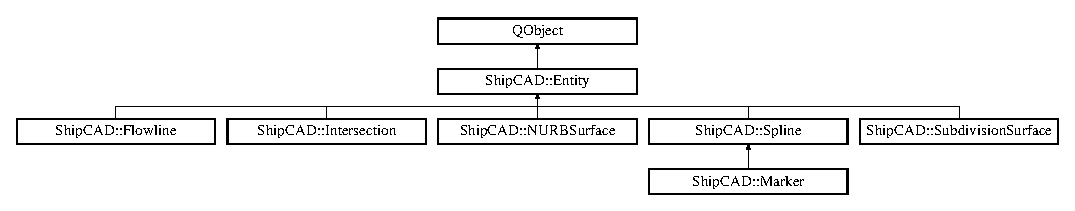
\includegraphics[height=3.589744cm]{classShipCAD_1_1Entity}
\end{center}
\end{figure}
\subsection*{Public Member Functions}
\begin{DoxyCompactItemize}
\item 
\hyperlink{classShipCAD_1_1Entity_a980f368aa07ce358583982821533a54a}{Entity} ()
\item 
virtual \hyperlink{classShipCAD_1_1Entity_a0fe3f9f7c8875a85afb214c8ebd75604}{$\sim$\-Entity} ()
\item 
virtual void \hyperlink{classShipCAD_1_1Entity_a998d0e5d360371046fd5835ba1e0877a}{clear} ()
\item 
virtual void \hyperlink{classShipCAD_1_1Entity_a08e8e53770c85002afa45f46e7bf10f8}{extents} (Q\-Vector3\-D \&min, Q\-Vector3\-D \&max)
\item 
virtual void \hyperlink{classShipCAD_1_1Entity_aa62e306d991140dcd564360f8f6e7539}{draw} (\hyperlink{classShipCAD_1_1Viewport}{Viewport} \&vp, \hyperlink{classShipCAD_1_1LineShader}{Line\-Shader} $\ast$lineshader)=0
\item 
virtual void \hyperlink{classShipCAD_1_1Entity_a2571654319df6ad6841a437be7a75395}{rebuild} ()=0
\item 
Q\-Vector3\-D \hyperlink{classShipCAD_1_1Entity_a759d6dedd36bf6562fbf36e816d9a5af}{get\-Min} ()
\item 
Q\-Vector3\-D \hyperlink{classShipCAD_1_1Entity_a3af98adafb45eb573675a8ccc44fe14e}{get\-Max} ()
\item 
bool \hyperlink{classShipCAD_1_1Entity_a131cd27d923ba1d2658528b679b9a90c}{is\-Build} ()
\item 
void \hyperlink{classShipCAD_1_1Entity_a395d7573df06482d9deaecdc87d46944}{dump} (std\-::ostream \&os) const 
\end{DoxyCompactItemize}
\subsection*{Protected Member Functions}
\begin{DoxyCompactItemize}
\item 
virtual void \hyperlink{classShipCAD_1_1Entity_a1889198398f42bb7f77a2334031c3f33}{set\-Build} (bool val)
\end{DoxyCompactItemize}
\subsection*{Protected Attributes}
\begin{DoxyCompactItemize}
\item 
bool \hyperlink{classShipCAD_1_1Entity_a752e3eb309111a7457783e0fdab3d6fe}{\-\_\-build}
\item 
Q\-Vector3\-D \hyperlink{classShipCAD_1_1Entity_a414d4ff1ee308d47a5052910c3b34f7b}{\-\_\-min}
\item 
Q\-Vector3\-D \hyperlink{classShipCAD_1_1Entity_a30e4f9cb421987cebd07737a554275eb}{\-\_\-max}
\item 
int \hyperlink{classShipCAD_1_1Entity_a5a9892a0d84d2cfdcd3a5dabf662a595}{\-\_\-pen\-\_\-width}
\item 
Q\-Color \hyperlink{classShipCAD_1_1Entity_a150a19aa958886e9dcf7c4e0e51dcd98}{\-\_\-color}
\item 
Qt\-::\-Pen\-Style \hyperlink{classShipCAD_1_1Entity_ac53123be976cd9739ad1657573d67d97}{\-\_\-pen\-\_\-style}
\end{DoxyCompactItemize}
\subsection*{Properties}
\begin{DoxyCompactItemize}
\item 
bool \hyperlink{classShipCAD_1_1Entity_a7518cde7c6a7c576827efd3d65c732e4}{Build}
\item 
Q\-Color \hyperlink{classShipCAD_1_1Entity_a117b8362d17e9ef352555a85a6f015ff}{Color}
\item 
Q\-Vector3\-D \hyperlink{classShipCAD_1_1Entity_ac363c3a8e4d5553b98996d6114b6b148}{Min}
\item 
Q\-Vector3\-D \hyperlink{classShipCAD_1_1Entity_a1ce317d1da352757209465baebce15f8}{Max}
\item 
int \hyperlink{classShipCAD_1_1Entity_a95a1cc38c08e5b64a540727afb99d25a}{Pen\-Width}
\item 
Qt\-::\-Pen\-Style \hyperlink{classShipCAD_1_1Entity_a8cbcbada188edd9d39e7c5743dc43560}{penstyle}
\end{DoxyCompactItemize}


\subsection{Detailed Description}


Definition at line 62 of file entity.\-h.



\subsection{Constructor \& Destructor Documentation}
\hypertarget{classShipCAD_1_1Entity_a980f368aa07ce358583982821533a54a}{\index{Ship\-C\-A\-D\-::\-Entity@{Ship\-C\-A\-D\-::\-Entity}!Entity@{Entity}}
\index{Entity@{Entity}!ShipCAD::Entity@{Ship\-C\-A\-D\-::\-Entity}}
\subsubsection[{Entity}]{\setlength{\rightskip}{0pt plus 5cm}Entity\-::\-Entity (
\begin{DoxyParamCaption}
{}
\end{DoxyParamCaption}
)\hspace{0.3cm}{\ttfamily [explicit]}}}\label{classShipCAD_1_1Entity_a980f368aa07ce358583982821533a54a}


Definition at line 42 of file entity.\-cpp.

\hypertarget{classShipCAD_1_1Entity_a0fe3f9f7c8875a85afb214c8ebd75604}{\index{Ship\-C\-A\-D\-::\-Entity@{Ship\-C\-A\-D\-::\-Entity}!$\sim$\-Entity@{$\sim$\-Entity}}
\index{$\sim$\-Entity@{$\sim$\-Entity}!ShipCAD::Entity@{Ship\-C\-A\-D\-::\-Entity}}
\subsubsection[{$\sim$\-Entity}]{\setlength{\rightskip}{0pt plus 5cm}virtual Ship\-C\-A\-D\-::\-Entity\-::$\sim$\-Entity (
\begin{DoxyParamCaption}
{}
\end{DoxyParamCaption}
)\hspace{0.3cm}{\ttfamily [inline]}, {\ttfamily [virtual]}}}\label{classShipCAD_1_1Entity_a0fe3f9f7c8875a85afb214c8ebd75604}


Definition at line 75 of file entity.\-h.



\subsection{Member Function Documentation}
\hypertarget{classShipCAD_1_1Entity_a998d0e5d360371046fd5835ba1e0877a}{\index{Ship\-C\-A\-D\-::\-Entity@{Ship\-C\-A\-D\-::\-Entity}!clear@{clear}}
\index{clear@{clear}!ShipCAD::Entity@{Ship\-C\-A\-D\-::\-Entity}}
\subsubsection[{clear}]{\setlength{\rightskip}{0pt plus 5cm}void Entity\-::clear (
\begin{DoxyParamCaption}
{}
\end{DoxyParamCaption}
)\hspace{0.3cm}{\ttfamily [virtual]}}}\label{classShipCAD_1_1Entity_a998d0e5d360371046fd5835ba1e0877a}


Reimplemented in \hyperlink{classShipCAD_1_1Spline_a02967f3eee8b1755eab0d7da55c3c621}{Ship\-C\-A\-D\-::\-Spline}, \hyperlink{classShipCAD_1_1Intersection_a2163245dc7153d1590811ab2902d6ee4}{Ship\-C\-A\-D\-::\-Intersection}, \hyperlink{classShipCAD_1_1Marker_ac7c7eea8648562f3fa00a9e10af6ec97}{Ship\-C\-A\-D\-::\-Marker}, \hyperlink{classShipCAD_1_1Flowline_a4e138d0d75b46f8ecb62a60ecf3f4e64}{Ship\-C\-A\-D\-::\-Flowline}, and \hyperlink{classShipCAD_1_1NURBSurface_a5013b0c1e511ea68909eef5d0473d032}{Ship\-C\-A\-D\-::\-N\-U\-R\-B\-Surface}.



Definition at line 47 of file entity.\-cpp.

\hypertarget{classShipCAD_1_1Entity_aa62e306d991140dcd564360f8f6e7539}{\index{Ship\-C\-A\-D\-::\-Entity@{Ship\-C\-A\-D\-::\-Entity}!draw@{draw}}
\index{draw@{draw}!ShipCAD::Entity@{Ship\-C\-A\-D\-::\-Entity}}
\subsubsection[{draw}]{\setlength{\rightskip}{0pt plus 5cm}virtual void Ship\-C\-A\-D\-::\-Entity\-::draw (
\begin{DoxyParamCaption}
\item[{{\bf Viewport} \&}]{vp, }
\item[{{\bf Line\-Shader} $\ast$}]{lineshader}
\end{DoxyParamCaption}
)\hspace{0.3cm}{\ttfamily [pure virtual]}}}\label{classShipCAD_1_1Entity_aa62e306d991140dcd564360f8f6e7539}


Implemented in \hyperlink{classShipCAD_1_1Spline_a6424ed433d241f566c15891cc25a74dd}{Ship\-C\-A\-D\-::\-Spline}, \hyperlink{classShipCAD_1_1Intersection_a9e346019a52aa0540628b75994ea94a5}{Ship\-C\-A\-D\-::\-Intersection}, \hyperlink{classShipCAD_1_1Flowline_afce93ff27acf72218b0e394b0d543a0d}{Ship\-C\-A\-D\-::\-Flowline}, and \hyperlink{classShipCAD_1_1Marker_a0cca647d9b32dc69b03903b024dc3091}{Ship\-C\-A\-D\-::\-Marker}.

\hypertarget{classShipCAD_1_1Entity_a395d7573df06482d9deaecdc87d46944}{\index{Ship\-C\-A\-D\-::\-Entity@{Ship\-C\-A\-D\-::\-Entity}!dump@{dump}}
\index{dump@{dump}!ShipCAD::Entity@{Ship\-C\-A\-D\-::\-Entity}}
\subsubsection[{dump}]{\setlength{\rightskip}{0pt plus 5cm}void Entity\-::dump (
\begin{DoxyParamCaption}
\item[{std\-::ostream \&}]{os}
\end{DoxyParamCaption}
) const}}\label{classShipCAD_1_1Entity_a395d7573df06482d9deaecdc87d46944}


Definition at line 95 of file entity.\-cpp.

\hypertarget{classShipCAD_1_1Entity_a08e8e53770c85002afa45f46e7bf10f8}{\index{Ship\-C\-A\-D\-::\-Entity@{Ship\-C\-A\-D\-::\-Entity}!extents@{extents}}
\index{extents@{extents}!ShipCAD::Entity@{Ship\-C\-A\-D\-::\-Entity}}
\subsubsection[{extents}]{\setlength{\rightskip}{0pt plus 5cm}void Entity\-::extents (
\begin{DoxyParamCaption}
\item[{Q\-Vector3\-D \&}]{min, }
\item[{Q\-Vector3\-D \&}]{max}
\end{DoxyParamCaption}
)\hspace{0.3cm}{\ttfamily [virtual]}}}\label{classShipCAD_1_1Entity_a08e8e53770c85002afa45f46e7bf10f8}


Reimplemented in \hyperlink{classShipCAD_1_1Intersection_af751d515708531ca098321840a92c47b}{Ship\-C\-A\-D\-::\-Intersection}, and \hyperlink{classShipCAD_1_1Flowline_abc8e875663d00a645f6d462cde7bff79}{Ship\-C\-A\-D\-::\-Flowline}.



Definition at line 57 of file entity.\-cpp.

\hypertarget{classShipCAD_1_1Entity_a3af98adafb45eb573675a8ccc44fe14e}{\index{Ship\-C\-A\-D\-::\-Entity@{Ship\-C\-A\-D\-::\-Entity}!get\-Max@{get\-Max}}
\index{get\-Max@{get\-Max}!ShipCAD::Entity@{Ship\-C\-A\-D\-::\-Entity}}
\subsubsection[{get\-Max}]{\setlength{\rightskip}{0pt plus 5cm}Q\-Vector3\-D Entity\-::get\-Max (
\begin{DoxyParamCaption}
{}
\end{DoxyParamCaption}
)}}\label{classShipCAD_1_1Entity_a3af98adafb45eb573675a8ccc44fe14e}


Definition at line 88 of file entity.\-cpp.

\hypertarget{classShipCAD_1_1Entity_a759d6dedd36bf6562fbf36e816d9a5af}{\index{Ship\-C\-A\-D\-::\-Entity@{Ship\-C\-A\-D\-::\-Entity}!get\-Min@{get\-Min}}
\index{get\-Min@{get\-Min}!ShipCAD::Entity@{Ship\-C\-A\-D\-::\-Entity}}
\subsubsection[{get\-Min}]{\setlength{\rightskip}{0pt plus 5cm}Q\-Vector3\-D Entity\-::get\-Min (
\begin{DoxyParamCaption}
{}
\end{DoxyParamCaption}
)}}\label{classShipCAD_1_1Entity_a759d6dedd36bf6562fbf36e816d9a5af}


Definition at line 81 of file entity.\-cpp.

\hypertarget{classShipCAD_1_1Entity_a131cd27d923ba1d2658528b679b9a90c}{\index{Ship\-C\-A\-D\-::\-Entity@{Ship\-C\-A\-D\-::\-Entity}!is\-Build@{is\-Build}}
\index{is\-Build@{is\-Build}!ShipCAD::Entity@{Ship\-C\-A\-D\-::\-Entity}}
\subsubsection[{is\-Build}]{\setlength{\rightskip}{0pt plus 5cm}bool Entity\-::is\-Build (
\begin{DoxyParamCaption}
{}
\end{DoxyParamCaption}
)}}\label{classShipCAD_1_1Entity_a131cd27d923ba1d2658528b679b9a90c}


Definition at line 65 of file entity.\-cpp.

\hypertarget{classShipCAD_1_1Entity_a2571654319df6ad6841a437be7a75395}{\index{Ship\-C\-A\-D\-::\-Entity@{Ship\-C\-A\-D\-::\-Entity}!rebuild@{rebuild}}
\index{rebuild@{rebuild}!ShipCAD::Entity@{Ship\-C\-A\-D\-::\-Entity}}
\subsubsection[{rebuild}]{\setlength{\rightskip}{0pt plus 5cm}virtual void Ship\-C\-A\-D\-::\-Entity\-::rebuild (
\begin{DoxyParamCaption}
{}
\end{DoxyParamCaption}
)\hspace{0.3cm}{\ttfamily [pure virtual]}}}\label{classShipCAD_1_1Entity_a2571654319df6ad6841a437be7a75395}


Implemented in \hyperlink{classShipCAD_1_1Spline_a9b466ad7510032dafb0421f2d834bde6}{Ship\-C\-A\-D\-::\-Spline}, \hyperlink{classShipCAD_1_1Intersection_aed30bdca43037f72b85c4d53e234fd6c}{Ship\-C\-A\-D\-::\-Intersection}, \hyperlink{classShipCAD_1_1Flowline_a13e27605271592ba288ad9d0b6e2a8c1}{Ship\-C\-A\-D\-::\-Flowline}, and \hyperlink{classShipCAD_1_1NURBSurface_a643231ea9a8f26e528a1d9a0dccf4070}{Ship\-C\-A\-D\-::\-N\-U\-R\-B\-Surface}.

\hypertarget{classShipCAD_1_1Entity_a1889198398f42bb7f77a2334031c3f33}{\index{Ship\-C\-A\-D\-::\-Entity@{Ship\-C\-A\-D\-::\-Entity}!set\-Build@{set\-Build}}
\index{set\-Build@{set\-Build}!ShipCAD::Entity@{Ship\-C\-A\-D\-::\-Entity}}
\subsubsection[{set\-Build}]{\setlength{\rightskip}{0pt plus 5cm}void Entity\-::set\-Build (
\begin{DoxyParamCaption}
\item[{bool}]{val}
\end{DoxyParamCaption}
)\hspace{0.3cm}{\ttfamily [protected]}, {\ttfamily [virtual]}}}\label{classShipCAD_1_1Entity_a1889198398f42bb7f77a2334031c3f33}


Reimplemented in \hyperlink{classShipCAD_1_1Spline_a6e932411f0f4463514f80011c58f5e6a}{Ship\-C\-A\-D\-::\-Spline}, \hyperlink{classShipCAD_1_1Intersection_a2b496f9ab21c5fc4a7b97a665b24f2b1}{Ship\-C\-A\-D\-::\-Intersection}, and \hyperlink{classShipCAD_1_1NURBSurface_aa6fc3d060087593349ce1b5119419433}{Ship\-C\-A\-D\-::\-N\-U\-R\-B\-Surface}.



Definition at line 70 of file entity.\-cpp.



\subsection{Member Data Documentation}
\hypertarget{classShipCAD_1_1Entity_a752e3eb309111a7457783e0fdab3d6fe}{\index{Ship\-C\-A\-D\-::\-Entity@{Ship\-C\-A\-D\-::\-Entity}!\-\_\-build@{\-\_\-build}}
\index{\-\_\-build@{\-\_\-build}!ShipCAD::Entity@{Ship\-C\-A\-D\-::\-Entity}}
\subsubsection[{\-\_\-build}]{\setlength{\rightskip}{0pt plus 5cm}bool Ship\-C\-A\-D\-::\-Entity\-::\-\_\-build\hspace{0.3cm}{\ttfamily [protected]}}}\label{classShipCAD_1_1Entity_a752e3eb309111a7457783e0fdab3d6fe}


Definition at line 96 of file entity.\-h.

\hypertarget{classShipCAD_1_1Entity_a150a19aa958886e9dcf7c4e0e51dcd98}{\index{Ship\-C\-A\-D\-::\-Entity@{Ship\-C\-A\-D\-::\-Entity}!\-\_\-color@{\-\_\-color}}
\index{\-\_\-color@{\-\_\-color}!ShipCAD::Entity@{Ship\-C\-A\-D\-::\-Entity}}
\subsubsection[{\-\_\-color}]{\setlength{\rightskip}{0pt plus 5cm}Q\-Color Ship\-C\-A\-D\-::\-Entity\-::\-\_\-color\hspace{0.3cm}{\ttfamily [protected]}}}\label{classShipCAD_1_1Entity_a150a19aa958886e9dcf7c4e0e51dcd98}


Definition at line 100 of file entity.\-h.

\hypertarget{classShipCAD_1_1Entity_a30e4f9cb421987cebd07737a554275eb}{\index{Ship\-C\-A\-D\-::\-Entity@{Ship\-C\-A\-D\-::\-Entity}!\-\_\-max@{\-\_\-max}}
\index{\-\_\-max@{\-\_\-max}!ShipCAD::Entity@{Ship\-C\-A\-D\-::\-Entity}}
\subsubsection[{\-\_\-max}]{\setlength{\rightskip}{0pt plus 5cm}Q\-Vector3\-D Ship\-C\-A\-D\-::\-Entity\-::\-\_\-max\hspace{0.3cm}{\ttfamily [protected]}}}\label{classShipCAD_1_1Entity_a30e4f9cb421987cebd07737a554275eb}


Definition at line 98 of file entity.\-h.

\hypertarget{classShipCAD_1_1Entity_a414d4ff1ee308d47a5052910c3b34f7b}{\index{Ship\-C\-A\-D\-::\-Entity@{Ship\-C\-A\-D\-::\-Entity}!\-\_\-min@{\-\_\-min}}
\index{\-\_\-min@{\-\_\-min}!ShipCAD::Entity@{Ship\-C\-A\-D\-::\-Entity}}
\subsubsection[{\-\_\-min}]{\setlength{\rightskip}{0pt plus 5cm}Q\-Vector3\-D Ship\-C\-A\-D\-::\-Entity\-::\-\_\-min\hspace{0.3cm}{\ttfamily [protected]}}}\label{classShipCAD_1_1Entity_a414d4ff1ee308d47a5052910c3b34f7b}


Definition at line 97 of file entity.\-h.

\hypertarget{classShipCAD_1_1Entity_ac53123be976cd9739ad1657573d67d97}{\index{Ship\-C\-A\-D\-::\-Entity@{Ship\-C\-A\-D\-::\-Entity}!\-\_\-pen\-\_\-style@{\-\_\-pen\-\_\-style}}
\index{\-\_\-pen\-\_\-style@{\-\_\-pen\-\_\-style}!ShipCAD::Entity@{Ship\-C\-A\-D\-::\-Entity}}
\subsubsection[{\-\_\-pen\-\_\-style}]{\setlength{\rightskip}{0pt plus 5cm}Qt\-::\-Pen\-Style Ship\-C\-A\-D\-::\-Entity\-::\-\_\-pen\-\_\-style\hspace{0.3cm}{\ttfamily [protected]}}}\label{classShipCAD_1_1Entity_ac53123be976cd9739ad1657573d67d97}


Definition at line 101 of file entity.\-h.

\hypertarget{classShipCAD_1_1Entity_a5a9892a0d84d2cfdcd3a5dabf662a595}{\index{Ship\-C\-A\-D\-::\-Entity@{Ship\-C\-A\-D\-::\-Entity}!\-\_\-pen\-\_\-width@{\-\_\-pen\-\_\-width}}
\index{\-\_\-pen\-\_\-width@{\-\_\-pen\-\_\-width}!ShipCAD::Entity@{Ship\-C\-A\-D\-::\-Entity}}
\subsubsection[{\-\_\-pen\-\_\-width}]{\setlength{\rightskip}{0pt plus 5cm}int Ship\-C\-A\-D\-::\-Entity\-::\-\_\-pen\-\_\-width\hspace{0.3cm}{\ttfamily [protected]}}}\label{classShipCAD_1_1Entity_a5a9892a0d84d2cfdcd3a5dabf662a595}


Definition at line 99 of file entity.\-h.



\subsection{Property Documentation}
\hypertarget{classShipCAD_1_1Entity_a7518cde7c6a7c576827efd3d65c732e4}{\index{Ship\-C\-A\-D\-::\-Entity@{Ship\-C\-A\-D\-::\-Entity}!Build@{Build}}
\index{Build@{Build}!ShipCAD::Entity@{Ship\-C\-A\-D\-::\-Entity}}
\subsubsection[{Build}]{\setlength{\rightskip}{0pt plus 5cm}bool Ship\-C\-A\-D\-::\-Entity\-::\-Build\hspace{0.3cm}{\ttfamily [read]}}}\label{classShipCAD_1_1Entity_a7518cde7c6a7c576827efd3d65c732e4}


Definition at line 65 of file entity.\-h.

\hypertarget{classShipCAD_1_1Entity_a117b8362d17e9ef352555a85a6f015ff}{\index{Ship\-C\-A\-D\-::\-Entity@{Ship\-C\-A\-D\-::\-Entity}!Color@{Color}}
\index{Color@{Color}!ShipCAD::Entity@{Ship\-C\-A\-D\-::\-Entity}}
\subsubsection[{Color}]{\setlength{\rightskip}{0pt plus 5cm}Q\-Color Ship\-C\-A\-D\-::\-Entity\-::\-Color}}\label{classShipCAD_1_1Entity_a117b8362d17e9ef352555a85a6f015ff}


Definition at line 66 of file entity.\-h.

\hypertarget{classShipCAD_1_1Entity_a1ce317d1da352757209465baebce15f8}{\index{Ship\-C\-A\-D\-::\-Entity@{Ship\-C\-A\-D\-::\-Entity}!Max@{Max}}
\index{Max@{Max}!ShipCAD::Entity@{Ship\-C\-A\-D\-::\-Entity}}
\subsubsection[{Max}]{\setlength{\rightskip}{0pt plus 5cm}Q\-Vector3\-D Ship\-C\-A\-D\-::\-Entity\-::\-Max\hspace{0.3cm}{\ttfamily [read]}}}\label{classShipCAD_1_1Entity_a1ce317d1da352757209465baebce15f8}


Definition at line 68 of file entity.\-h.

\hypertarget{classShipCAD_1_1Entity_ac363c3a8e4d5553b98996d6114b6b148}{\index{Ship\-C\-A\-D\-::\-Entity@{Ship\-C\-A\-D\-::\-Entity}!Min@{Min}}
\index{Min@{Min}!ShipCAD::Entity@{Ship\-C\-A\-D\-::\-Entity}}
\subsubsection[{Min}]{\setlength{\rightskip}{0pt plus 5cm}Q\-Vector3\-D Ship\-C\-A\-D\-::\-Entity\-::\-Min\hspace{0.3cm}{\ttfamily [read]}}}\label{classShipCAD_1_1Entity_ac363c3a8e4d5553b98996d6114b6b148}


Definition at line 67 of file entity.\-h.

\hypertarget{classShipCAD_1_1Entity_a8cbcbada188edd9d39e7c5743dc43560}{\index{Ship\-C\-A\-D\-::\-Entity@{Ship\-C\-A\-D\-::\-Entity}!penstyle@{penstyle}}
\index{penstyle@{penstyle}!ShipCAD::Entity@{Ship\-C\-A\-D\-::\-Entity}}
\subsubsection[{penstyle}]{\setlength{\rightskip}{0pt plus 5cm}Qt\-::\-Pen\-Style Ship\-C\-A\-D\-::\-Entity\-::penstyle}}\label{classShipCAD_1_1Entity_a8cbcbada188edd9d39e7c5743dc43560}


Definition at line 70 of file entity.\-h.

\hypertarget{classShipCAD_1_1Entity_a95a1cc38c08e5b64a540727afb99d25a}{\index{Ship\-C\-A\-D\-::\-Entity@{Ship\-C\-A\-D\-::\-Entity}!Pen\-Width@{Pen\-Width}}
\index{Pen\-Width@{Pen\-Width}!ShipCAD::Entity@{Ship\-C\-A\-D\-::\-Entity}}
\subsubsection[{Pen\-Width}]{\setlength{\rightskip}{0pt plus 5cm}int Ship\-C\-A\-D\-::\-Entity\-::\-Pen\-Width}}\label{classShipCAD_1_1Entity_a95a1cc38c08e5b64a540727afb99d25a}


Definition at line 69 of file entity.\-h.



The documentation for this class was generated from the following files\-:\begin{DoxyCompactItemize}
\item 
Ship\-C\-A\-Dlib/\hyperlink{entity_8h}{entity.\-h}\item 
Ship\-C\-A\-Dlib/\hyperlink{entity_8cpp}{entity.\-cpp}\end{DoxyCompactItemize}

\hypertarget{structExistPointPred}{\section{Exist\-Point\-Pred Struct Reference}
\label{structExistPointPred}\index{Exist\-Point\-Pred@{Exist\-Point\-Pred}}
}
\subsection*{Public Member Functions}
\begin{DoxyCompactItemize}
\item 
bool \hyperlink{structExistPointPred_a349fa048c84af089053c09f0ac76325b}{operator()} (const pair$<$ \hyperlink{classShipCAD_1_1SubdivisionControlPoint}{Ship\-C\-A\-D\-::\-Subdivision\-Control\-Point} $\ast$, \hyperlink{classShipCAD_1_1SubdivisionControlPoint}{Ship\-C\-A\-D\-::\-Subdivision\-Control\-Point} $\ast$ $>$ \&val)
\item 
\hyperlink{structExistPointPred_a7e596a35605dc5f710f6ea9a2e07eed2}{Exist\-Point\-Pred} (\hyperlink{classShipCAD_1_1SubdivisionPoint}{Ship\-C\-A\-D\-::\-Subdivision\-Point} $\ast$querypt)
\end{DoxyCompactItemize}
\subsection*{Public Attributes}
\begin{DoxyCompactItemize}
\item 
\hyperlink{classShipCAD_1_1SubdivisionControlPoint}{Ship\-C\-A\-D\-::\-Subdivision\-Control\-Point} $\ast$ \hyperlink{structExistPointPred_a237f009691af455ff164985c3ab80901}{\-\_\-querypt}
\end{DoxyCompactItemize}


\subsection{Detailed Description}


Definition at line 1396 of file subdivsurface.\-cpp.



\subsection{Constructor \& Destructor Documentation}
\hypertarget{structExistPointPred_a7e596a35605dc5f710f6ea9a2e07eed2}{\index{Exist\-Point\-Pred@{Exist\-Point\-Pred}!Exist\-Point\-Pred@{Exist\-Point\-Pred}}
\index{Exist\-Point\-Pred@{Exist\-Point\-Pred}!ExistPointPred@{Exist\-Point\-Pred}}
\subsubsection[{Exist\-Point\-Pred}]{\setlength{\rightskip}{0pt plus 5cm}Exist\-Point\-Pred\-::\-Exist\-Point\-Pred (
\begin{DoxyParamCaption}
\item[{{\bf Ship\-C\-A\-D\-::\-Subdivision\-Point} $\ast$}]{querypt}
\end{DoxyParamCaption}
)\hspace{0.3cm}{\ttfamily [inline]}}}\label{structExistPointPred_a7e596a35605dc5f710f6ea9a2e07eed2}


Definition at line 1402 of file subdivsurface.\-cpp.



\subsection{Member Function Documentation}
\hypertarget{structExistPointPred_a349fa048c84af089053c09f0ac76325b}{\index{Exist\-Point\-Pred@{Exist\-Point\-Pred}!operator()@{operator()}}
\index{operator()@{operator()}!ExistPointPred@{Exist\-Point\-Pred}}
\subsubsection[{operator()}]{\setlength{\rightskip}{0pt plus 5cm}bool Exist\-Point\-Pred\-::operator() (
\begin{DoxyParamCaption}
\item[{const pair$<$ {\bf Ship\-C\-A\-D\-::\-Subdivision\-Control\-Point} $\ast$, {\bf Ship\-C\-A\-D\-::\-Subdivision\-Control\-Point} $\ast$ $>$ \&}]{val}
\end{DoxyParamCaption}
)\hspace{0.3cm}{\ttfamily [inline]}}}\label{structExistPointPred_a349fa048c84af089053c09f0ac76325b}


Definition at line 1398 of file subdivsurface.\-cpp.



\subsection{Member Data Documentation}
\hypertarget{structExistPointPred_a237f009691af455ff164985c3ab80901}{\index{Exist\-Point\-Pred@{Exist\-Point\-Pred}!\-\_\-querypt@{\-\_\-querypt}}
\index{\-\_\-querypt@{\-\_\-querypt}!ExistPointPred@{Exist\-Point\-Pred}}
\subsubsection[{\-\_\-querypt}]{\setlength{\rightskip}{0pt plus 5cm}{\bf Ship\-C\-A\-D\-::\-Subdivision\-Control\-Point}$\ast$ Exist\-Point\-Pred\-::\-\_\-querypt}}\label{structExistPointPred_a237f009691af455ff164985c3ab80901}


Definition at line 1397 of file subdivsurface.\-cpp.



The documentation for this struct was generated from the following file\-:\begin{DoxyCompactItemize}
\item 
Ship\-C\-A\-Dlib/\hyperlink{subdivsurface_8cpp}{subdivsurface.\-cpp}\end{DoxyCompactItemize}

\hypertarget{structExtrudePointPred}{\section{Extrude\-Point\-Pred Struct Reference}
\label{structExtrudePointPred}\index{Extrude\-Point\-Pred@{Extrude\-Point\-Pred}}
}
\subsection*{Public Member Functions}
\begin{DoxyCompactItemize}
\item 
bool \hyperlink{structExtrudePointPred_ab8901a2a46f147e81c80c25b0492c772}{operator()} (const pair$<$ \hyperlink{classShipCAD_1_1SubdivisionControlPoint}{Ship\-C\-A\-D\-::\-Subdivision\-Control\-Point} $\ast$, \hyperlink{classShipCAD_1_1SubdivisionControlPoint}{Ship\-C\-A\-D\-::\-Subdivision\-Control\-Point} $\ast$ $>$ \&val)
\item 
\hyperlink{structExtrudePointPred_ac213b3b8d1bdc5a72e0a5a4ed53d9439}{Extrude\-Point\-Pred} (\hyperlink{classShipCAD_1_1SubdivisionPoint}{Ship\-C\-A\-D\-::\-Subdivision\-Point} $\ast$querypt)
\end{DoxyCompactItemize}
\subsection*{Public Attributes}
\begin{DoxyCompactItemize}
\item 
\hyperlink{classShipCAD_1_1SubdivisionControlPoint}{Ship\-C\-A\-D\-::\-Subdivision\-Control\-Point} $\ast$ \hyperlink{structExtrudePointPred_af9fa40238ef74aca6b8f8d7e303aafb4}{\-\_\-querypt}
\end{DoxyCompactItemize}


\subsection{Detailed Description}


Definition at line 1941 of file subdivsurface.\-cpp.



\subsection{Constructor \& Destructor Documentation}
\hypertarget{structExtrudePointPred_ac213b3b8d1bdc5a72e0a5a4ed53d9439}{\index{Extrude\-Point\-Pred@{Extrude\-Point\-Pred}!Extrude\-Point\-Pred@{Extrude\-Point\-Pred}}
\index{Extrude\-Point\-Pred@{Extrude\-Point\-Pred}!ExtrudePointPred@{Extrude\-Point\-Pred}}
\subsubsection[{Extrude\-Point\-Pred}]{\setlength{\rightskip}{0pt plus 5cm}Extrude\-Point\-Pred\-::\-Extrude\-Point\-Pred (
\begin{DoxyParamCaption}
\item[{{\bf Ship\-C\-A\-D\-::\-Subdivision\-Point} $\ast$}]{querypt}
\end{DoxyParamCaption}
)\hspace{0.3cm}{\ttfamily [inline]}}}\label{structExtrudePointPred_ac213b3b8d1bdc5a72e0a5a4ed53d9439}


Definition at line 1947 of file subdivsurface.\-cpp.



\subsection{Member Function Documentation}
\hypertarget{structExtrudePointPred_ab8901a2a46f147e81c80c25b0492c772}{\index{Extrude\-Point\-Pred@{Extrude\-Point\-Pred}!operator()@{operator()}}
\index{operator()@{operator()}!ExtrudePointPred@{Extrude\-Point\-Pred}}
\subsubsection[{operator()}]{\setlength{\rightskip}{0pt plus 5cm}bool Extrude\-Point\-Pred\-::operator() (
\begin{DoxyParamCaption}
\item[{const pair$<$ {\bf Ship\-C\-A\-D\-::\-Subdivision\-Control\-Point} $\ast$, {\bf Ship\-C\-A\-D\-::\-Subdivision\-Control\-Point} $\ast$ $>$ \&}]{val}
\end{DoxyParamCaption}
)\hspace{0.3cm}{\ttfamily [inline]}}}\label{structExtrudePointPred_ab8901a2a46f147e81c80c25b0492c772}


Definition at line 1943 of file subdivsurface.\-cpp.



\subsection{Member Data Documentation}
\hypertarget{structExtrudePointPred_af9fa40238ef74aca6b8f8d7e303aafb4}{\index{Extrude\-Point\-Pred@{Extrude\-Point\-Pred}!\-\_\-querypt@{\-\_\-querypt}}
\index{\-\_\-querypt@{\-\_\-querypt}!ExtrudePointPred@{Extrude\-Point\-Pred}}
\subsubsection[{\-\_\-querypt}]{\setlength{\rightskip}{0pt plus 5cm}{\bf Ship\-C\-A\-D\-::\-Subdivision\-Control\-Point}$\ast$ Extrude\-Point\-Pred\-::\-\_\-querypt}}\label{structExtrudePointPred_af9fa40238ef74aca6b8f8d7e303aafb4}


Definition at line 1942 of file subdivsurface.\-cpp.



The documentation for this struct was generated from the following file\-:\begin{DoxyCompactItemize}
\item 
Ship\-C\-A\-Dlib/\hyperlink{subdivsurface_8cpp}{subdivsurface.\-cpp}\end{DoxyCompactItemize}

\hypertarget{structFacePred}{\section{Face\-Pred Struct Reference}
\label{structFacePred}\index{Face\-Pred@{Face\-Pred}}
}
\subsection*{Public Member Functions}
\begin{DoxyCompactItemize}
\item 
bool \hyperlink{structFacePred_a6abdd4cf5e1665459109f92abbba8e43}{operator()} (const pair$<$ \hyperlink{classShipCAD_1_1SubdivisionFace}{Ship\-C\-A\-D\-::\-Subdivision\-Face} $\ast$, \hyperlink{classShipCAD_1_1SubdivisionPoint}{Ship\-C\-A\-D\-::\-Subdivision\-Point} $\ast$ $>$ \&val)
\item 
\hyperlink{structFacePred_a8ce3462c74c45932241e934da4048a65}{Face\-Pred} (\hyperlink{classShipCAD_1_1SubdivisionFace}{Ship\-C\-A\-D\-::\-Subdivision\-Face} $\ast$queryface)
\end{DoxyCompactItemize}
\subsection*{Public Attributes}
\begin{DoxyCompactItemize}
\item 
\hyperlink{classShipCAD_1_1SubdivisionFace}{Ship\-C\-A\-D\-::\-Subdivision\-Face} $\ast$ \hyperlink{structFacePred_abe2d14d3f749323559d7a06b06ca99a8}{\-\_\-queryface}
\end{DoxyCompactItemize}


\subsection{Detailed Description}


Definition at line 239 of file subdivface.\-cpp.



\subsection{Constructor \& Destructor Documentation}
\hypertarget{structFacePred_a8ce3462c74c45932241e934da4048a65}{\index{Face\-Pred@{Face\-Pred}!Face\-Pred@{Face\-Pred}}
\index{Face\-Pred@{Face\-Pred}!FacePred@{Face\-Pred}}
\subsubsection[{Face\-Pred}]{\setlength{\rightskip}{0pt plus 5cm}Face\-Pred\-::\-Face\-Pred (
\begin{DoxyParamCaption}
\item[{{\bf Ship\-C\-A\-D\-::\-Subdivision\-Face} $\ast$}]{queryface}
\end{DoxyParamCaption}
)\hspace{0.3cm}{\ttfamily [inline]}}}\label{structFacePred_a8ce3462c74c45932241e934da4048a65}


Definition at line 245 of file subdivface.\-cpp.



\subsection{Member Function Documentation}
\hypertarget{structFacePred_a6abdd4cf5e1665459109f92abbba8e43}{\index{Face\-Pred@{Face\-Pred}!operator()@{operator()}}
\index{operator()@{operator()}!FacePred@{Face\-Pred}}
\subsubsection[{operator()}]{\setlength{\rightskip}{0pt plus 5cm}bool Face\-Pred\-::operator() (
\begin{DoxyParamCaption}
\item[{const pair$<$ {\bf Ship\-C\-A\-D\-::\-Subdivision\-Face} $\ast$, {\bf Ship\-C\-A\-D\-::\-Subdivision\-Point} $\ast$ $>$ \&}]{val}
\end{DoxyParamCaption}
)\hspace{0.3cm}{\ttfamily [inline]}}}\label{structFacePred_a6abdd4cf5e1665459109f92abbba8e43}


Definition at line 241 of file subdivface.\-cpp.



\subsection{Member Data Documentation}
\hypertarget{structFacePred_abe2d14d3f749323559d7a06b06ca99a8}{\index{Face\-Pred@{Face\-Pred}!\-\_\-queryface@{\-\_\-queryface}}
\index{\-\_\-queryface@{\-\_\-queryface}!FacePred@{Face\-Pred}}
\subsubsection[{\-\_\-queryface}]{\setlength{\rightskip}{0pt plus 5cm}{\bf Ship\-C\-A\-D\-::\-Subdivision\-Face}$\ast$ Face\-Pred\-::\-\_\-queryface}}\label{structFacePred_abe2d14d3f749323559d7a06b06ca99a8}


Definition at line 240 of file subdivface.\-cpp.



The documentation for this struct was generated from the following file\-:\begin{DoxyCompactItemize}
\item 
Ship\-C\-A\-Dlib/\hyperlink{subdivface_8cpp}{subdivface.\-cpp}\end{DoxyCompactItemize}

\hypertarget{classShipCAD_1_1FileBuffer}{\section{Ship\-C\-A\-D\-:\-:File\-Buffer Class Reference}
\label{classShipCAD_1_1FileBuffer}\index{Ship\-C\-A\-D\-::\-File\-Buffer@{Ship\-C\-A\-D\-::\-File\-Buffer}}
}


in-\/memory buffer of data for a binary file (F\-R\-E\-E!\-Ship format)  




{\ttfamily \#include $<$filebuffer.\-h$>$}

Inheritance diagram for Ship\-C\-A\-D\-:\-:File\-Buffer\-:\begin{figure}[H]
\begin{center}
\leavevmode
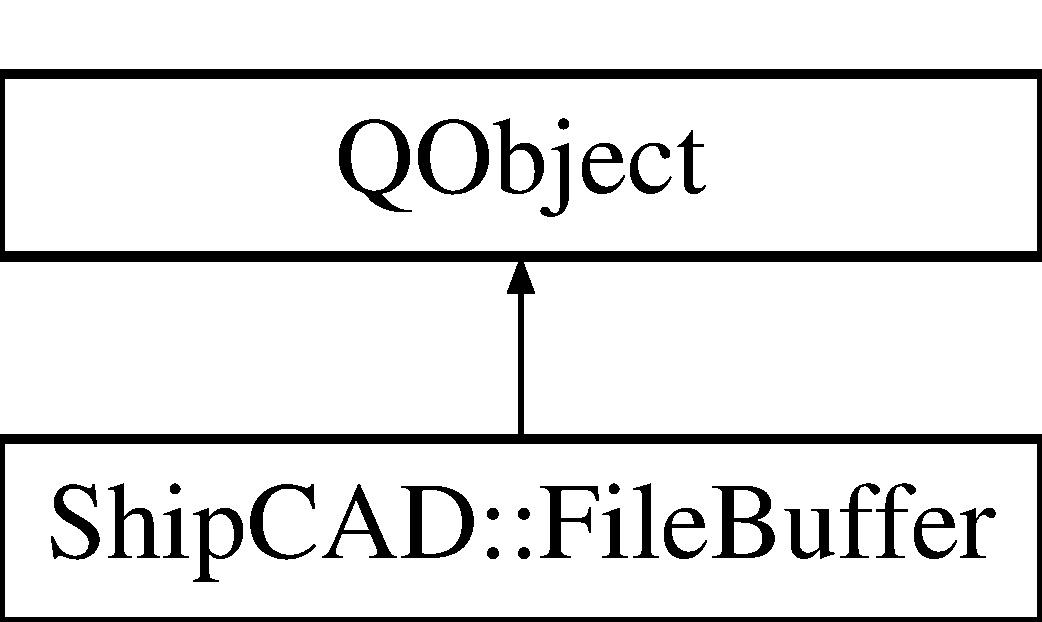
\includegraphics[height=2.000000cm]{classShipCAD_1_1FileBuffer}
\end{center}
\end{figure}
\subsection*{Public Member Functions}
\begin{DoxyCompactItemize}
\item 
\hyperlink{classShipCAD_1_1FileBuffer_ab243cfcb8a68ce791103594e974ee9ba}{File\-Buffer} ()
\item 
\hyperlink{classShipCAD_1_1FileBuffer_a397c9a755598f9939eb30460b605d44c}{$\sim$\-File\-Buffer} ()
\item 
size\-\_\-t \hyperlink{classShipCAD_1_1FileBuffer_a51dc1007457d999ce374afd6a6ae29f8}{size} ()
\item 
\hyperlink{namespaceShipCAD_af3a6fa23a7318acbda7b0066b53d694f}{version\-\_\-t} \hyperlink{classShipCAD_1_1FileBuffer_a06f87b30f5fd091cc5c270964ea16770}{get\-Version} ()
\item 
void \hyperlink{classShipCAD_1_1FileBuffer_a66c14f8f21b9f77febd154aee9565f0b}{set\-Version} (\hyperlink{namespaceShipCAD_af3a6fa23a7318acbda7b0066b53d694f}{version\-\_\-t} v)
\item 
void \hyperlink{classShipCAD_1_1FileBuffer_a7d5d6ac5aa85545999186f4745a77093}{load\-From\-File} (const Q\-String \&filename)
\item 
void \hyperlink{classShipCAD_1_1FileBuffer_a175d7a153228b5cba5db062a2afd5026}{save\-To\-File} (const Q\-String \&filename)
\item 
void \hyperlink{classShipCAD_1_1FileBuffer_af59c26297994b38aabc4bc678d04c246}{reset} ()
\item 
void \hyperlink{classShipCAD_1_1FileBuffer_a86223c54bcf111ef205c9d651e0b9a66}{load} (\hyperlink{structShipCAD_1_1JPEGImage}{J\-P\-E\-G\-Image} \&img)
\item 
void \hyperlink{classShipCAD_1_1FileBuffer_a9a5d46b2c6d568ee2cdef110d4773e73}{add} (const \hyperlink{structShipCAD_1_1JPEGImage}{J\-P\-E\-G\-Image} \&img)
\item 
void \hyperlink{classShipCAD_1_1FileBuffer_ab196d459581b5c877ebea2f567e9bda8}{load} (quint8 \&val)
\item 
void \hyperlink{classShipCAD_1_1FileBuffer_afb11c583e5d3a7a580e5f88004d6c7e3}{add} (quint8 val)
\item 
void \hyperlink{classShipCAD_1_1FileBuffer_ad1aebcc97e364569934c66eec5a87485}{load} (bool \&val)
\item 
void \hyperlink{classShipCAD_1_1FileBuffer_a7cb4395eae7ffa405290c3bed9890bee}{add} (bool val)
\item 
void \hyperlink{classShipCAD_1_1FileBuffer_a525306d68a017ef67ec13c3e8901a8ff}{load} (float \&val)
\item 
void \hyperlink{classShipCAD_1_1FileBuffer_a7909794ac33ad5f695bb670940db99ba}{add} (float val)
\item 
void \hyperlink{classShipCAD_1_1FileBuffer_ad7fc82d31f73f0350715fb63db2fc271}{load} (qint32 \&val)
\item 
void \hyperlink{classShipCAD_1_1FileBuffer_ad5ff9b7299df09feb365250c69e6da9a}{add} (qint32 val)
\item 
void \hyperlink{classShipCAD_1_1FileBuffer_a19fcd1363671552150de3d6ee3297f2c}{load} (quint32 \&val)
\item 
void \hyperlink{classShipCAD_1_1FileBuffer_a1dd1963dd35caff15333f21cc2195b34}{add} (quint32 val)
\item 
void \hyperlink{classShipCAD_1_1FileBuffer_aa22983fa24559f6d0d119d89036100af}{add} (size\-\_\-t val)
\begin{DoxyCompactList}\small\item\em save value, (check that it fits in 32 bits) \end{DoxyCompactList}\item 
void \hyperlink{classShipCAD_1_1FileBuffer_a7255342a053689ebafda9317cc586c57}{load} (Q\-Vector3\-D \&val)
\item 
void \hyperlink{classShipCAD_1_1FileBuffer_a0642733d14682981c12f6aeaef9bb884}{add} (const Q\-Vector3\-D \&val)
\item 
void \hyperlink{classShipCAD_1_1FileBuffer_a3329cf81740c79967acc24bc0ac3c9a3}{load} (Q\-Color \&val)
\item 
void \hyperlink{classShipCAD_1_1FileBuffer_a3611327a77cc938e987ecda018d0d936}{add} (const Q\-Color \&val)
\item 
void \hyperlink{classShipCAD_1_1FileBuffer_a82c790d09c8e85c0f9d218efd9c93605}{load} (Q\-String \&val)
\item 
void \hyperlink{classShipCAD_1_1FileBuffer_aea305be34bc316cc5b849fb291499012}{add} (const Q\-String \&val)
\item 
void \hyperlink{classShipCAD_1_1FileBuffer_a4ae77da0ea26a1ed6de262ff7f3d606f}{load} (\hyperlink{classShipCAD_1_1Plane}{Plane} \&val)
\item 
void \hyperlink{classShipCAD_1_1FileBuffer_ae947c5bac13749a8b0d833bfa7979d0d}{add} (const \hyperlink{classShipCAD_1_1Plane}{Plane} \&val)
\item 
void \hyperlink{classShipCAD_1_1FileBuffer_acfa1ad9b776baa948d1724bd56b4e18d}{load} (\hyperlink{structShipCAD_1_1DelftSeriesResistance}{Delft\-Series\-Resistance} $\ast$buf)
\item 
void \hyperlink{classShipCAD_1_1FileBuffer_a63b2793d04b55d67ef7a307e664b3416}{add} (const \hyperlink{structShipCAD_1_1DelftSeriesResistance}{Delft\-Series\-Resistance} $\ast$buf)
\item 
void \hyperlink{classShipCAD_1_1FileBuffer_aec2753a3f1fb3aab1303a8dfde26bb1c}{load} (\hyperlink{structShipCAD_1_1KAPERResistance}{K\-A\-P\-E\-R\-Resistance} $\ast$buf)
\item 
void \hyperlink{classShipCAD_1_1FileBuffer_a1189100c2022918351d730590d107c33}{add} (const \hyperlink{structShipCAD_1_1KAPERResistance}{K\-A\-P\-E\-R\-Resistance} $\ast$buf)
\end{DoxyCompactItemize}


\subsection{Detailed Description}
in-\/memory buffer of data for a binary file (F\-R\-E\-E!\-Ship format) 

Definition at line 52 of file filebuffer.\-h.



\subsection{Constructor \& Destructor Documentation}
\hypertarget{classShipCAD_1_1FileBuffer_ab243cfcb8a68ce791103594e974ee9ba}{\index{Ship\-C\-A\-D\-::\-File\-Buffer@{Ship\-C\-A\-D\-::\-File\-Buffer}!File\-Buffer@{File\-Buffer}}
\index{File\-Buffer@{File\-Buffer}!ShipCAD::FileBuffer@{Ship\-C\-A\-D\-::\-File\-Buffer}}
\subsubsection[{File\-Buffer}]{\setlength{\rightskip}{0pt plus 5cm}File\-Buffer\-::\-File\-Buffer (
\begin{DoxyParamCaption}
{}
\end{DoxyParamCaption}
)\hspace{0.3cm}{\ttfamily [explicit]}}}\label{classShipCAD_1_1FileBuffer_ab243cfcb8a68ce791103594e974ee9ba}


Definition at line 50 of file filebuffer.\-cpp.

\hypertarget{classShipCAD_1_1FileBuffer_a397c9a755598f9939eb30460b605d44c}{\index{Ship\-C\-A\-D\-::\-File\-Buffer@{Ship\-C\-A\-D\-::\-File\-Buffer}!$\sim$\-File\-Buffer@{$\sim$\-File\-Buffer}}
\index{$\sim$\-File\-Buffer@{$\sim$\-File\-Buffer}!ShipCAD::FileBuffer@{Ship\-C\-A\-D\-::\-File\-Buffer}}
\subsubsection[{$\sim$\-File\-Buffer}]{\setlength{\rightskip}{0pt plus 5cm}Ship\-C\-A\-D\-::\-File\-Buffer\-::$\sim$\-File\-Buffer (
\begin{DoxyParamCaption}
{}
\end{DoxyParamCaption}
)\hspace{0.3cm}{\ttfamily [inline]}}}\label{classShipCAD_1_1FileBuffer_a397c9a755598f9939eb30460b605d44c}


Definition at line 58 of file filebuffer.\-h.



\subsection{Member Function Documentation}
\hypertarget{classShipCAD_1_1FileBuffer_a9a5d46b2c6d568ee2cdef110d4773e73}{\index{Ship\-C\-A\-D\-::\-File\-Buffer@{Ship\-C\-A\-D\-::\-File\-Buffer}!add@{add}}
\index{add@{add}!ShipCAD::FileBuffer@{Ship\-C\-A\-D\-::\-File\-Buffer}}
\subsubsection[{add}]{\setlength{\rightskip}{0pt plus 5cm}void File\-Buffer\-::add (
\begin{DoxyParamCaption}
\item[{const {\bf J\-P\-E\-G\-Image} \&}]{img}
\end{DoxyParamCaption}
)}}\label{classShipCAD_1_1FileBuffer_a9a5d46b2c6d568ee2cdef110d4773e73}


Definition at line 105 of file filebuffer.\-cpp.

\hypertarget{classShipCAD_1_1FileBuffer_afb11c583e5d3a7a580e5f88004d6c7e3}{\index{Ship\-C\-A\-D\-::\-File\-Buffer@{Ship\-C\-A\-D\-::\-File\-Buffer}!add@{add}}
\index{add@{add}!ShipCAD::FileBuffer@{Ship\-C\-A\-D\-::\-File\-Buffer}}
\subsubsection[{add}]{\setlength{\rightskip}{0pt plus 5cm}void File\-Buffer\-::add (
\begin{DoxyParamCaption}
\item[{quint8}]{val}
\end{DoxyParamCaption}
)}}\label{classShipCAD_1_1FileBuffer_afb11c583e5d3a7a580e5f88004d6c7e3}


Definition at line 116 of file filebuffer.\-cpp.

\hypertarget{classShipCAD_1_1FileBuffer_a7cb4395eae7ffa405290c3bed9890bee}{\index{Ship\-C\-A\-D\-::\-File\-Buffer@{Ship\-C\-A\-D\-::\-File\-Buffer}!add@{add}}
\index{add@{add}!ShipCAD::FileBuffer@{Ship\-C\-A\-D\-::\-File\-Buffer}}
\subsubsection[{add}]{\setlength{\rightskip}{0pt plus 5cm}void File\-Buffer\-::add (
\begin{DoxyParamCaption}
\item[{bool}]{val}
\end{DoxyParamCaption}
)}}\label{classShipCAD_1_1FileBuffer_a7cb4395eae7ffa405290c3bed9890bee}


Definition at line 129 of file filebuffer.\-cpp.

\hypertarget{classShipCAD_1_1FileBuffer_a7909794ac33ad5f695bb670940db99ba}{\index{Ship\-C\-A\-D\-::\-File\-Buffer@{Ship\-C\-A\-D\-::\-File\-Buffer}!add@{add}}
\index{add@{add}!ShipCAD::FileBuffer@{Ship\-C\-A\-D\-::\-File\-Buffer}}
\subsubsection[{add}]{\setlength{\rightskip}{0pt plus 5cm}void File\-Buffer\-::add (
\begin{DoxyParamCaption}
\item[{float}]{val}
\end{DoxyParamCaption}
)}}\label{classShipCAD_1_1FileBuffer_a7909794ac33ad5f695bb670940db99ba}


Definition at line 143 of file filebuffer.\-cpp.

\hypertarget{classShipCAD_1_1FileBuffer_ad5ff9b7299df09feb365250c69e6da9a}{\index{Ship\-C\-A\-D\-::\-File\-Buffer@{Ship\-C\-A\-D\-::\-File\-Buffer}!add@{add}}
\index{add@{add}!ShipCAD::FileBuffer@{Ship\-C\-A\-D\-::\-File\-Buffer}}
\subsubsection[{add}]{\setlength{\rightskip}{0pt plus 5cm}void File\-Buffer\-::add (
\begin{DoxyParamCaption}
\item[{qint32}]{val}
\end{DoxyParamCaption}
)}}\label{classShipCAD_1_1FileBuffer_ad5ff9b7299df09feb365250c69e6da9a}


Definition at line 160 of file filebuffer.\-cpp.

\hypertarget{classShipCAD_1_1FileBuffer_a1dd1963dd35caff15333f21cc2195b34}{\index{Ship\-C\-A\-D\-::\-File\-Buffer@{Ship\-C\-A\-D\-::\-File\-Buffer}!add@{add}}
\index{add@{add}!ShipCAD::FileBuffer@{Ship\-C\-A\-D\-::\-File\-Buffer}}
\subsubsection[{add}]{\setlength{\rightskip}{0pt plus 5cm}void File\-Buffer\-::add (
\begin{DoxyParamCaption}
\item[{quint32}]{val}
\end{DoxyParamCaption}
)}}\label{classShipCAD_1_1FileBuffer_a1dd1963dd35caff15333f21cc2195b34}


Definition at line 177 of file filebuffer.\-cpp.

\hypertarget{classShipCAD_1_1FileBuffer_aa22983fa24559f6d0d119d89036100af}{\index{Ship\-C\-A\-D\-::\-File\-Buffer@{Ship\-C\-A\-D\-::\-File\-Buffer}!add@{add}}
\index{add@{add}!ShipCAD::FileBuffer@{Ship\-C\-A\-D\-::\-File\-Buffer}}
\subsubsection[{add}]{\setlength{\rightskip}{0pt plus 5cm}void File\-Buffer\-::add (
\begin{DoxyParamCaption}
\item[{size\-\_\-t}]{val}
\end{DoxyParamCaption}
)}}\label{classShipCAD_1_1FileBuffer_aa22983fa24559f6d0d119d89036100af}


save value, (check that it fits in 32 bits) 


\begin{DoxyParams}{Parameters}
{\em val} & integer to save \\
\hline
\end{DoxyParams}

\begin{DoxyExceptions}{Exceptions}
{\em range\-\_\-error} & if val is greater than 32bit unsigned \\
\hline
\end{DoxyExceptions}


Definition at line 185 of file filebuffer.\-cpp.

\hypertarget{classShipCAD_1_1FileBuffer_a0642733d14682981c12f6aeaef9bb884}{\index{Ship\-C\-A\-D\-::\-File\-Buffer@{Ship\-C\-A\-D\-::\-File\-Buffer}!add@{add}}
\index{add@{add}!ShipCAD::FileBuffer@{Ship\-C\-A\-D\-::\-File\-Buffer}}
\subsubsection[{add}]{\setlength{\rightskip}{0pt plus 5cm}void File\-Buffer\-::add (
\begin{DoxyParamCaption}
\item[{const Q\-Vector3\-D \&}]{val}
\end{DoxyParamCaption}
)}}\label{classShipCAD_1_1FileBuffer_a0642733d14682981c12f6aeaef9bb884}


Definition at line 228 of file filebuffer.\-cpp.

\hypertarget{classShipCAD_1_1FileBuffer_a3611327a77cc938e987ecda018d0d936}{\index{Ship\-C\-A\-D\-::\-File\-Buffer@{Ship\-C\-A\-D\-::\-File\-Buffer}!add@{add}}
\index{add@{add}!ShipCAD::FileBuffer@{Ship\-C\-A\-D\-::\-File\-Buffer}}
\subsubsection[{add}]{\setlength{\rightskip}{0pt plus 5cm}void File\-Buffer\-::add (
\begin{DoxyParamCaption}
\item[{const Q\-Color \&}]{val}
\end{DoxyParamCaption}
)}}\label{classShipCAD_1_1FileBuffer_a3611327a77cc938e987ecda018d0d936}


Definition at line 195 of file filebuffer.\-cpp.

\hypertarget{classShipCAD_1_1FileBuffer_aea305be34bc316cc5b849fb291499012}{\index{Ship\-C\-A\-D\-::\-File\-Buffer@{Ship\-C\-A\-D\-::\-File\-Buffer}!add@{add}}
\index{add@{add}!ShipCAD::FileBuffer@{Ship\-C\-A\-D\-::\-File\-Buffer}}
\subsubsection[{add}]{\setlength{\rightskip}{0pt plus 5cm}void File\-Buffer\-::add (
\begin{DoxyParamCaption}
\item[{const Q\-String \&}]{val}
\end{DoxyParamCaption}
)}}\label{classShipCAD_1_1FileBuffer_aea305be34bc316cc5b849fb291499012}


Definition at line 257 of file filebuffer.\-cpp.

\hypertarget{classShipCAD_1_1FileBuffer_ae947c5bac13749a8b0d833bfa7979d0d}{\index{Ship\-C\-A\-D\-::\-File\-Buffer@{Ship\-C\-A\-D\-::\-File\-Buffer}!add@{add}}
\index{add@{add}!ShipCAD::FileBuffer@{Ship\-C\-A\-D\-::\-File\-Buffer}}
\subsubsection[{add}]{\setlength{\rightskip}{0pt plus 5cm}void File\-Buffer\-::add (
\begin{DoxyParamCaption}
\item[{const {\bf Plane} \&}]{val}
\end{DoxyParamCaption}
)}}\label{classShipCAD_1_1FileBuffer_ae947c5bac13749a8b0d833bfa7979d0d}


Definition at line 287 of file filebuffer.\-cpp.

\hypertarget{classShipCAD_1_1FileBuffer_a63b2793d04b55d67ef7a307e664b3416}{\index{Ship\-C\-A\-D\-::\-File\-Buffer@{Ship\-C\-A\-D\-::\-File\-Buffer}!add@{add}}
\index{add@{add}!ShipCAD::FileBuffer@{Ship\-C\-A\-D\-::\-File\-Buffer}}
\subsubsection[{add}]{\setlength{\rightskip}{0pt plus 5cm}void File\-Buffer\-::add (
\begin{DoxyParamCaption}
\item[{const {\bf Delft\-Series\-Resistance} $\ast$}]{buf}
\end{DoxyParamCaption}
)}}\label{classShipCAD_1_1FileBuffer_a63b2793d04b55d67ef7a307e664b3416}


Definition at line 312 of file filebuffer.\-cpp.

\hypertarget{classShipCAD_1_1FileBuffer_a1189100c2022918351d730590d107c33}{\index{Ship\-C\-A\-D\-::\-File\-Buffer@{Ship\-C\-A\-D\-::\-File\-Buffer}!add@{add}}
\index{add@{add}!ShipCAD::FileBuffer@{Ship\-C\-A\-D\-::\-File\-Buffer}}
\subsubsection[{add}]{\setlength{\rightskip}{0pt plus 5cm}void File\-Buffer\-::add (
\begin{DoxyParamCaption}
\item[{const {\bf K\-A\-P\-E\-R\-Resistance} $\ast$}]{buf}
\end{DoxyParamCaption}
)}}\label{classShipCAD_1_1FileBuffer_a1189100c2022918351d730590d107c33}


Definition at line 327 of file filebuffer.\-cpp.

\hypertarget{classShipCAD_1_1FileBuffer_a06f87b30f5fd091cc5c270964ea16770}{\index{Ship\-C\-A\-D\-::\-File\-Buffer@{Ship\-C\-A\-D\-::\-File\-Buffer}!get\-Version@{get\-Version}}
\index{get\-Version@{get\-Version}!ShipCAD::FileBuffer@{Ship\-C\-A\-D\-::\-File\-Buffer}}
\subsubsection[{get\-Version}]{\setlength{\rightskip}{0pt plus 5cm}{\bf version\-\_\-t} Ship\-C\-A\-D\-::\-File\-Buffer\-::get\-Version (
\begin{DoxyParamCaption}
{}
\end{DoxyParamCaption}
)\hspace{0.3cm}{\ttfamily [inline]}}}\label{classShipCAD_1_1FileBuffer_a06f87b30f5fd091cc5c270964ea16770}


Definition at line 63 of file filebuffer.\-h.

\hypertarget{classShipCAD_1_1FileBuffer_a86223c54bcf111ef205c9d651e0b9a66}{\index{Ship\-C\-A\-D\-::\-File\-Buffer@{Ship\-C\-A\-D\-::\-File\-Buffer}!load@{load}}
\index{load@{load}!ShipCAD::FileBuffer@{Ship\-C\-A\-D\-::\-File\-Buffer}}
\subsubsection[{load}]{\setlength{\rightskip}{0pt plus 5cm}void File\-Buffer\-::load (
\begin{DoxyParamCaption}
\item[{{\bf J\-P\-E\-G\-Image} \&}]{img}
\end{DoxyParamCaption}
)}}\label{classShipCAD_1_1FileBuffer_a86223c54bcf111ef205c9d651e0b9a66}


Definition at line 96 of file filebuffer.\-cpp.

\hypertarget{classShipCAD_1_1FileBuffer_ab196d459581b5c877ebea2f567e9bda8}{\index{Ship\-C\-A\-D\-::\-File\-Buffer@{Ship\-C\-A\-D\-::\-File\-Buffer}!load@{load}}
\index{load@{load}!ShipCAD::FileBuffer@{Ship\-C\-A\-D\-::\-File\-Buffer}}
\subsubsection[{load}]{\setlength{\rightskip}{0pt plus 5cm}void File\-Buffer\-::load (
\begin{DoxyParamCaption}
\item[{quint8 \&}]{val}
\end{DoxyParamCaption}
)}}\label{classShipCAD_1_1FileBuffer_ab196d459581b5c877ebea2f567e9bda8}


Definition at line 110 of file filebuffer.\-cpp.

\hypertarget{classShipCAD_1_1FileBuffer_ad1aebcc97e364569934c66eec5a87485}{\index{Ship\-C\-A\-D\-::\-File\-Buffer@{Ship\-C\-A\-D\-::\-File\-Buffer}!load@{load}}
\index{load@{load}!ShipCAD::FileBuffer@{Ship\-C\-A\-D\-::\-File\-Buffer}}
\subsubsection[{load}]{\setlength{\rightskip}{0pt plus 5cm}void File\-Buffer\-::load (
\begin{DoxyParamCaption}
\item[{bool \&}]{val}
\end{DoxyParamCaption}
)}}\label{classShipCAD_1_1FileBuffer_ad1aebcc97e364569934c66eec5a87485}


Definition at line 121 of file filebuffer.\-cpp.

\hypertarget{classShipCAD_1_1FileBuffer_a525306d68a017ef67ec13c3e8901a8ff}{\index{Ship\-C\-A\-D\-::\-File\-Buffer@{Ship\-C\-A\-D\-::\-File\-Buffer}!load@{load}}
\index{load@{load}!ShipCAD::FileBuffer@{Ship\-C\-A\-D\-::\-File\-Buffer}}
\subsubsection[{load}]{\setlength{\rightskip}{0pt plus 5cm}void File\-Buffer\-::load (
\begin{DoxyParamCaption}
\item[{float \&}]{val}
\end{DoxyParamCaption}
)}}\label{classShipCAD_1_1FileBuffer_a525306d68a017ef67ec13c3e8901a8ff}


Definition at line 134 of file filebuffer.\-cpp.

\hypertarget{classShipCAD_1_1FileBuffer_ad7fc82d31f73f0350715fb63db2fc271}{\index{Ship\-C\-A\-D\-::\-File\-Buffer@{Ship\-C\-A\-D\-::\-File\-Buffer}!load@{load}}
\index{load@{load}!ShipCAD::FileBuffer@{Ship\-C\-A\-D\-::\-File\-Buffer}}
\subsubsection[{load}]{\setlength{\rightskip}{0pt plus 5cm}void File\-Buffer\-::load (
\begin{DoxyParamCaption}
\item[{qint32 \&}]{val}
\end{DoxyParamCaption}
)}}\label{classShipCAD_1_1FileBuffer_ad7fc82d31f73f0350715fb63db2fc271}


Definition at line 151 of file filebuffer.\-cpp.

\hypertarget{classShipCAD_1_1FileBuffer_a19fcd1363671552150de3d6ee3297f2c}{\index{Ship\-C\-A\-D\-::\-File\-Buffer@{Ship\-C\-A\-D\-::\-File\-Buffer}!load@{load}}
\index{load@{load}!ShipCAD::FileBuffer@{Ship\-C\-A\-D\-::\-File\-Buffer}}
\subsubsection[{load}]{\setlength{\rightskip}{0pt plus 5cm}void File\-Buffer\-::load (
\begin{DoxyParamCaption}
\item[{quint32 \&}]{val}
\end{DoxyParamCaption}
)}}\label{classShipCAD_1_1FileBuffer_a19fcd1363671552150de3d6ee3297f2c}


Definition at line 168 of file filebuffer.\-cpp.

\hypertarget{classShipCAD_1_1FileBuffer_a7255342a053689ebafda9317cc586c57}{\index{Ship\-C\-A\-D\-::\-File\-Buffer@{Ship\-C\-A\-D\-::\-File\-Buffer}!load@{load}}
\index{load@{load}!ShipCAD::FileBuffer@{Ship\-C\-A\-D\-::\-File\-Buffer}}
\subsubsection[{load}]{\setlength{\rightskip}{0pt plus 5cm}void File\-Buffer\-::load (
\begin{DoxyParamCaption}
\item[{Q\-Vector3\-D \&}]{val}
\end{DoxyParamCaption}
)}}\label{classShipCAD_1_1FileBuffer_a7255342a053689ebafda9317cc586c57}


Definition at line 213 of file filebuffer.\-cpp.

\hypertarget{classShipCAD_1_1FileBuffer_a3329cf81740c79967acc24bc0ac3c9a3}{\index{Ship\-C\-A\-D\-::\-File\-Buffer@{Ship\-C\-A\-D\-::\-File\-Buffer}!load@{load}}
\index{load@{load}!ShipCAD::FileBuffer@{Ship\-C\-A\-D\-::\-File\-Buffer}}
\subsubsection[{load}]{\setlength{\rightskip}{0pt plus 5cm}void File\-Buffer\-::load (
\begin{DoxyParamCaption}
\item[{Q\-Color \&}]{val}
\end{DoxyParamCaption}
)}}\label{classShipCAD_1_1FileBuffer_a3329cf81740c79967acc24bc0ac3c9a3}


Definition at line 203 of file filebuffer.\-cpp.

\hypertarget{classShipCAD_1_1FileBuffer_a82c790d09c8e85c0f9d218efd9c93605}{\index{Ship\-C\-A\-D\-::\-File\-Buffer@{Ship\-C\-A\-D\-::\-File\-Buffer}!load@{load}}
\index{load@{load}!ShipCAD::FileBuffer@{Ship\-C\-A\-D\-::\-File\-Buffer}}
\subsubsection[{load}]{\setlength{\rightskip}{0pt plus 5cm}void File\-Buffer\-::load (
\begin{DoxyParamCaption}
\item[{Q\-String \&}]{val}
\end{DoxyParamCaption}
)}}\label{classShipCAD_1_1FileBuffer_a82c790d09c8e85c0f9d218efd9c93605}


Definition at line 242 of file filebuffer.\-cpp.

\hypertarget{classShipCAD_1_1FileBuffer_a4ae77da0ea26a1ed6de262ff7f3d606f}{\index{Ship\-C\-A\-D\-::\-File\-Buffer@{Ship\-C\-A\-D\-::\-File\-Buffer}!load@{load}}
\index{load@{load}!ShipCAD::FileBuffer@{Ship\-C\-A\-D\-::\-File\-Buffer}}
\subsubsection[{load}]{\setlength{\rightskip}{0pt plus 5cm}void File\-Buffer\-::load (
\begin{DoxyParamCaption}
\item[{{\bf Plane} \&}]{val}
\end{DoxyParamCaption}
)}}\label{classShipCAD_1_1FileBuffer_a4ae77da0ea26a1ed6de262ff7f3d606f}


Definition at line 269 of file filebuffer.\-cpp.

\hypertarget{classShipCAD_1_1FileBuffer_acfa1ad9b776baa948d1724bd56b4e18d}{\index{Ship\-C\-A\-D\-::\-File\-Buffer@{Ship\-C\-A\-D\-::\-File\-Buffer}!load@{load}}
\index{load@{load}!ShipCAD::FileBuffer@{Ship\-C\-A\-D\-::\-File\-Buffer}}
\subsubsection[{load}]{\setlength{\rightskip}{0pt plus 5cm}void File\-Buffer\-::load (
\begin{DoxyParamCaption}
\item[{{\bf Delft\-Series\-Resistance} $\ast$}]{buf}
\end{DoxyParamCaption}
)}}\label{classShipCAD_1_1FileBuffer_acfa1ad9b776baa948d1724bd56b4e18d}


Definition at line 304 of file filebuffer.\-cpp.

\hypertarget{classShipCAD_1_1FileBuffer_aec2753a3f1fb3aab1303a8dfde26bb1c}{\index{Ship\-C\-A\-D\-::\-File\-Buffer@{Ship\-C\-A\-D\-::\-File\-Buffer}!load@{load}}
\index{load@{load}!ShipCAD::FileBuffer@{Ship\-C\-A\-D\-::\-File\-Buffer}}
\subsubsection[{load}]{\setlength{\rightskip}{0pt plus 5cm}void File\-Buffer\-::load (
\begin{DoxyParamCaption}
\item[{{\bf K\-A\-P\-E\-R\-Resistance} $\ast$}]{buf}
\end{DoxyParamCaption}
)}}\label{classShipCAD_1_1FileBuffer_aec2753a3f1fb3aab1303a8dfde26bb1c}


Definition at line 319 of file filebuffer.\-cpp.

\hypertarget{classShipCAD_1_1FileBuffer_a7d5d6ac5aa85545999186f4745a77093}{\index{Ship\-C\-A\-D\-::\-File\-Buffer@{Ship\-C\-A\-D\-::\-File\-Buffer}!load\-From\-File@{load\-From\-File}}
\index{load\-From\-File@{load\-From\-File}!ShipCAD::FileBuffer@{Ship\-C\-A\-D\-::\-File\-Buffer}}
\subsubsection[{load\-From\-File}]{\setlength{\rightskip}{0pt plus 5cm}void File\-Buffer\-::load\-From\-File (
\begin{DoxyParamCaption}
\item[{const Q\-String \&}]{filename}
\end{DoxyParamCaption}
)}}\label{classShipCAD_1_1FileBuffer_a7d5d6ac5aa85545999186f4745a77093}


Definition at line 66 of file filebuffer.\-cpp.

\hypertarget{classShipCAD_1_1FileBuffer_af59c26297994b38aabc4bc678d04c246}{\index{Ship\-C\-A\-D\-::\-File\-Buffer@{Ship\-C\-A\-D\-::\-File\-Buffer}!reset@{reset}}
\index{reset@{reset}!ShipCAD::FileBuffer@{Ship\-C\-A\-D\-::\-File\-Buffer}}
\subsubsection[{reset}]{\setlength{\rightskip}{0pt plus 5cm}void File\-Buffer\-::reset (
\begin{DoxyParamCaption}
{}
\end{DoxyParamCaption}
)}}\label{classShipCAD_1_1FileBuffer_af59c26297994b38aabc4bc678d04c246}


Definition at line 56 of file filebuffer.\-cpp.

\hypertarget{classShipCAD_1_1FileBuffer_a175d7a153228b5cba5db062a2afd5026}{\index{Ship\-C\-A\-D\-::\-File\-Buffer@{Ship\-C\-A\-D\-::\-File\-Buffer}!save\-To\-File@{save\-To\-File}}
\index{save\-To\-File@{save\-To\-File}!ShipCAD::FileBuffer@{Ship\-C\-A\-D\-::\-File\-Buffer}}
\subsubsection[{save\-To\-File}]{\setlength{\rightskip}{0pt plus 5cm}void File\-Buffer\-::save\-To\-File (
\begin{DoxyParamCaption}
\item[{const Q\-String \&}]{filename}
\end{DoxyParamCaption}
)}}\label{classShipCAD_1_1FileBuffer_a175d7a153228b5cba5db062a2afd5026}


Definition at line 84 of file filebuffer.\-cpp.

\hypertarget{classShipCAD_1_1FileBuffer_a66c14f8f21b9f77febd154aee9565f0b}{\index{Ship\-C\-A\-D\-::\-File\-Buffer@{Ship\-C\-A\-D\-::\-File\-Buffer}!set\-Version@{set\-Version}}
\index{set\-Version@{set\-Version}!ShipCAD::FileBuffer@{Ship\-C\-A\-D\-::\-File\-Buffer}}
\subsubsection[{set\-Version}]{\setlength{\rightskip}{0pt plus 5cm}void File\-Buffer\-::set\-Version (
\begin{DoxyParamCaption}
\item[{{\bf version\-\_\-t}}]{v}
\end{DoxyParamCaption}
)}}\label{classShipCAD_1_1FileBuffer_a66c14f8f21b9f77febd154aee9565f0b}


Definition at line 61 of file filebuffer.\-cpp.

\hypertarget{classShipCAD_1_1FileBuffer_a51dc1007457d999ce374afd6a6ae29f8}{\index{Ship\-C\-A\-D\-::\-File\-Buffer@{Ship\-C\-A\-D\-::\-File\-Buffer}!size@{size}}
\index{size@{size}!ShipCAD::FileBuffer@{Ship\-C\-A\-D\-::\-File\-Buffer}}
\subsubsection[{size}]{\setlength{\rightskip}{0pt plus 5cm}size\-\_\-t Ship\-C\-A\-D\-::\-File\-Buffer\-::size (
\begin{DoxyParamCaption}
{}
\end{DoxyParamCaption}
)\hspace{0.3cm}{\ttfamily [inline]}}}\label{classShipCAD_1_1FileBuffer_a51dc1007457d999ce374afd6a6ae29f8}


Definition at line 60 of file filebuffer.\-h.



The documentation for this class was generated from the following files\-:\begin{DoxyCompactItemize}
\item 
Ship\-C\-A\-Dlib/\hyperlink{filebuffer_8h}{filebuffer.\-h}\item 
Ship\-C\-A\-Dlib/\hyperlink{filebuffer_8cpp}{filebuffer.\-cpp}\end{DoxyCompactItemize}

\hypertarget{classShipCAD_1_1Flowline}{\section{Ship\-C\-A\-D\-:\-:Flowline Class Reference}
\label{classShipCAD_1_1Flowline}\index{Ship\-C\-A\-D\-::\-Flowline@{Ship\-C\-A\-D\-::\-Flowline}}
}


{\ttfamily \#include $<$flowline.\-h$>$}

Inheritance diagram for Ship\-C\-A\-D\-:\-:Flowline\-:\begin{figure}[H]
\begin{center}
\leavevmode
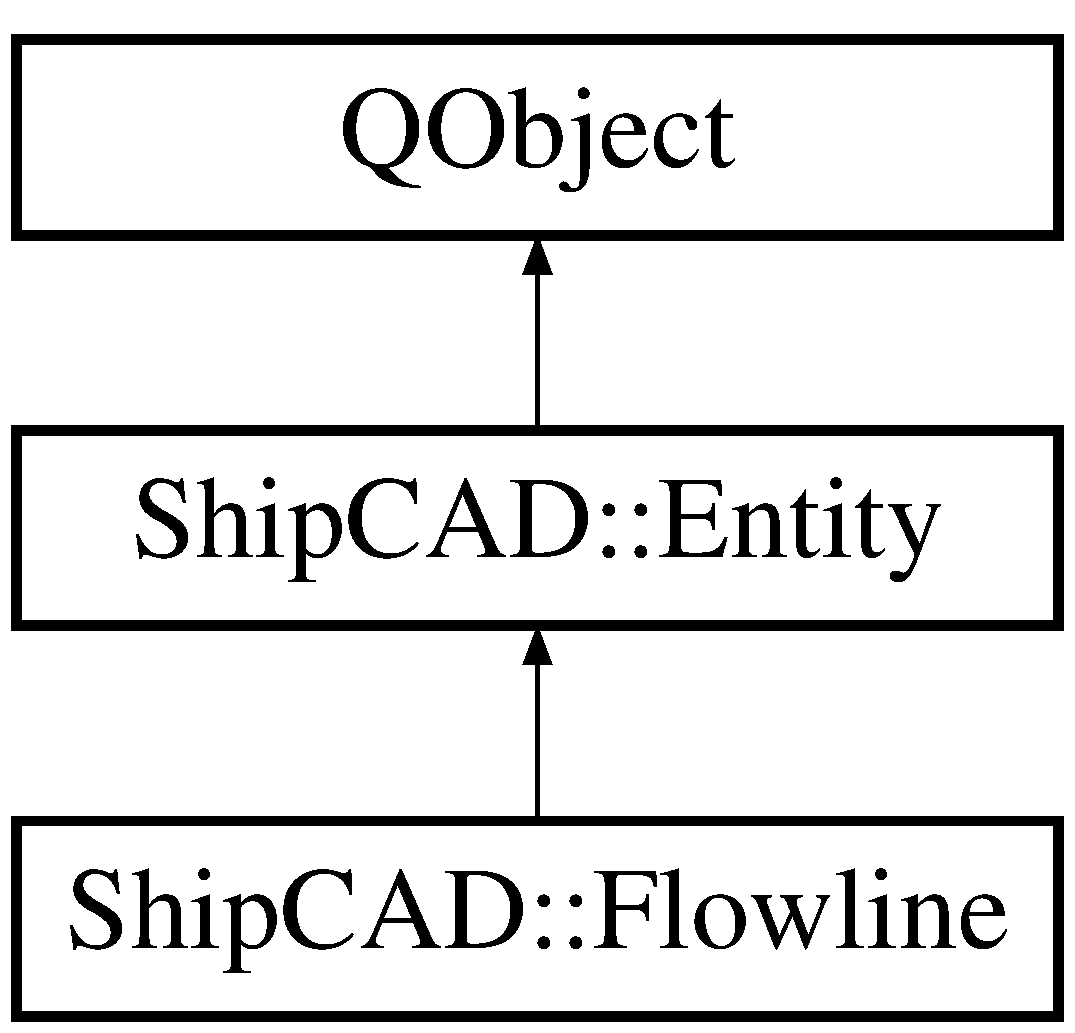
\includegraphics[height=3.000000cm]{classShipCAD_1_1Flowline}
\end{center}
\end{figure}
\subsection*{Public Member Functions}
\begin{DoxyCompactItemize}
\item 
\hyperlink{classShipCAD_1_1Flowline_a736d6251cea3c3b290416a27159cad96}{Flowline} (Ship\-C\-A\-D $\ast$owner)
\item 
virtual \hyperlink{classShipCAD_1_1Flowline_a77555e4dc8db9f99b684ea60e2a1a88e}{$\sim$\-Flowline} ()
\item 
virtual void \hyperlink{classShipCAD_1_1Flowline_a4e138d0d75b46f8ecb62a60ecf3f4e64}{clear} ()
\item 
virtual void \hyperlink{classShipCAD_1_1Flowline_abc8e875663d00a645f6d462cde7bff79}{extents} (Q\-Vector3\-D \&min, Q\-Vector3\-D \&max)
\item 
virtual void \hyperlink{classShipCAD_1_1Flowline_afce93ff27acf72218b0e394b0d543a0d}{draw} (\hyperlink{classShipCAD_1_1Viewport}{Viewport} \&vp, \hyperlink{classShipCAD_1_1LineShader}{Line\-Shader} $\ast$lineshader)
\item 
virtual void \hyperlink{classShipCAD_1_1Flowline_a13e27605271592ba288ad9d0b6e2a8c1}{rebuild} ()
\item 
bool \hyperlink{classShipCAD_1_1Flowline_aaaf96bde2aff35bd302ebf4e784b6a04}{is\-Visible} ()
\item 
void \hyperlink{classShipCAD_1_1Flowline_ad6546bfd621882e9d5067c919e148871}{set\-Visible} (bool set)
\item 
bool \hyperlink{classShipCAD_1_1Flowline_af2daefa9893fef5c56b398d01be529af}{is\-Selected} ()
\item 
void \hyperlink{classShipCAD_1_1Flowline_af8205e548dba009fd1a169f0a841dde5}{set\-Selected} (bool set)
\item 
void \hyperlink{classShipCAD_1_1Flowline_ad852ac9d0cf1ec68ad7243c19aed6410}{load\-Binary} (\hyperlink{classShipCAD_1_1FileBuffer}{File\-Buffer} \&buf)
\item 
void \hyperlink{classShipCAD_1_1Flowline_ae36a33c0140e03676ccc1f90ceb53543}{save\-Binary} (\hyperlink{classShipCAD_1_1FileBuffer}{File\-Buffer} \&buf)
\end{DoxyCompactItemize}
\subsection*{Static Public Member Functions}
\begin{DoxyCompactItemize}
\item 
static \hyperlink{classShipCAD_1_1Flowline}{Flowline} $\ast$ \hyperlink{classShipCAD_1_1Flowline_aadb39af0ba334958a3596b464f81006b}{construct} (Ship\-C\-A\-D $\ast$owner)
\end{DoxyCompactItemize}
\subsection*{Additional Inherited Members}


\subsection{Detailed Description}


Definition at line 46 of file flowline.\-h.



\subsection{Constructor \& Destructor Documentation}
\hypertarget{classShipCAD_1_1Flowline_a736d6251cea3c3b290416a27159cad96}{\index{Ship\-C\-A\-D\-::\-Flowline@{Ship\-C\-A\-D\-::\-Flowline}!Flowline@{Flowline}}
\index{Flowline@{Flowline}!ShipCAD::Flowline@{Ship\-C\-A\-D\-::\-Flowline}}
\subsubsection[{Flowline}]{\setlength{\rightskip}{0pt plus 5cm}Ship\-C\-A\-D\-::\-Flowline\-::\-Flowline (
\begin{DoxyParamCaption}
\item[{Ship\-C\-A\-D $\ast$}]{owner}
\end{DoxyParamCaption}
)\hspace{0.3cm}{\ttfamily [explicit]}}}\label{classShipCAD_1_1Flowline_a736d6251cea3c3b290416a27159cad96}
\hypertarget{classShipCAD_1_1Flowline_a77555e4dc8db9f99b684ea60e2a1a88e}{\index{Ship\-C\-A\-D\-::\-Flowline@{Ship\-C\-A\-D\-::\-Flowline}!$\sim$\-Flowline@{$\sim$\-Flowline}}
\index{$\sim$\-Flowline@{$\sim$\-Flowline}!ShipCAD::Flowline@{Ship\-C\-A\-D\-::\-Flowline}}
\subsubsection[{$\sim$\-Flowline}]{\setlength{\rightskip}{0pt plus 5cm}virtual Ship\-C\-A\-D\-::\-Flowline\-::$\sim$\-Flowline (
\begin{DoxyParamCaption}
{}
\end{DoxyParamCaption}
)\hspace{0.3cm}{\ttfamily [virtual]}}}\label{classShipCAD_1_1Flowline_a77555e4dc8db9f99b684ea60e2a1a88e}


\subsection{Member Function Documentation}
\hypertarget{classShipCAD_1_1Flowline_a4e138d0d75b46f8ecb62a60ecf3f4e64}{\index{Ship\-C\-A\-D\-::\-Flowline@{Ship\-C\-A\-D\-::\-Flowline}!clear@{clear}}
\index{clear@{clear}!ShipCAD::Flowline@{Ship\-C\-A\-D\-::\-Flowline}}
\subsubsection[{clear}]{\setlength{\rightskip}{0pt plus 5cm}virtual void Ship\-C\-A\-D\-::\-Flowline\-::clear (
\begin{DoxyParamCaption}
{}
\end{DoxyParamCaption}
)\hspace{0.3cm}{\ttfamily [virtual]}}}\label{classShipCAD_1_1Flowline_a4e138d0d75b46f8ecb62a60ecf3f4e64}


Reimplemented from \hyperlink{classShipCAD_1_1Entity_a998d0e5d360371046fd5835ba1e0877a}{Ship\-C\-A\-D\-::\-Entity}.

\hypertarget{classShipCAD_1_1Flowline_aadb39af0ba334958a3596b464f81006b}{\index{Ship\-C\-A\-D\-::\-Flowline@{Ship\-C\-A\-D\-::\-Flowline}!construct@{construct}}
\index{construct@{construct}!ShipCAD::Flowline@{Ship\-C\-A\-D\-::\-Flowline}}
\subsubsection[{construct}]{\setlength{\rightskip}{0pt plus 5cm}static {\bf Flowline}$\ast$ Ship\-C\-A\-D\-::\-Flowline\-::construct (
\begin{DoxyParamCaption}
\item[{Ship\-C\-A\-D $\ast$}]{owner}
\end{DoxyParamCaption}
)\hspace{0.3cm}{\ttfamily [static]}}}\label{classShipCAD_1_1Flowline_aadb39af0ba334958a3596b464f81006b}
\hypertarget{classShipCAD_1_1Flowline_afce93ff27acf72218b0e394b0d543a0d}{\index{Ship\-C\-A\-D\-::\-Flowline@{Ship\-C\-A\-D\-::\-Flowline}!draw@{draw}}
\index{draw@{draw}!ShipCAD::Flowline@{Ship\-C\-A\-D\-::\-Flowline}}
\subsubsection[{draw}]{\setlength{\rightskip}{0pt plus 5cm}virtual void Ship\-C\-A\-D\-::\-Flowline\-::draw (
\begin{DoxyParamCaption}
\item[{{\bf Viewport} \&}]{vp, }
\item[{{\bf Line\-Shader} $\ast$}]{lineshader}
\end{DoxyParamCaption}
)\hspace{0.3cm}{\ttfamily [virtual]}}}\label{classShipCAD_1_1Flowline_afce93ff27acf72218b0e394b0d543a0d}


Implements \hyperlink{classShipCAD_1_1Entity_aa62e306d991140dcd564360f8f6e7539}{Ship\-C\-A\-D\-::\-Entity}.

\hypertarget{classShipCAD_1_1Flowline_abc8e875663d00a645f6d462cde7bff79}{\index{Ship\-C\-A\-D\-::\-Flowline@{Ship\-C\-A\-D\-::\-Flowline}!extents@{extents}}
\index{extents@{extents}!ShipCAD::Flowline@{Ship\-C\-A\-D\-::\-Flowline}}
\subsubsection[{extents}]{\setlength{\rightskip}{0pt plus 5cm}virtual void Ship\-C\-A\-D\-::\-Flowline\-::extents (
\begin{DoxyParamCaption}
\item[{Q\-Vector3\-D \&}]{min, }
\item[{Q\-Vector3\-D \&}]{max}
\end{DoxyParamCaption}
)\hspace{0.3cm}{\ttfamily [virtual]}}}\label{classShipCAD_1_1Flowline_abc8e875663d00a645f6d462cde7bff79}


Reimplemented from \hyperlink{classShipCAD_1_1Entity_a08e8e53770c85002afa45f46e7bf10f8}{Ship\-C\-A\-D\-::\-Entity}.

\hypertarget{classShipCAD_1_1Flowline_af2daefa9893fef5c56b398d01be529af}{\index{Ship\-C\-A\-D\-::\-Flowline@{Ship\-C\-A\-D\-::\-Flowline}!is\-Selected@{is\-Selected}}
\index{is\-Selected@{is\-Selected}!ShipCAD::Flowline@{Ship\-C\-A\-D\-::\-Flowline}}
\subsubsection[{is\-Selected}]{\setlength{\rightskip}{0pt plus 5cm}bool Ship\-C\-A\-D\-::\-Flowline\-::is\-Selected (
\begin{DoxyParamCaption}
{}
\end{DoxyParamCaption}
)}}\label{classShipCAD_1_1Flowline_af2daefa9893fef5c56b398d01be529af}
\hypertarget{classShipCAD_1_1Flowline_aaaf96bde2aff35bd302ebf4e784b6a04}{\index{Ship\-C\-A\-D\-::\-Flowline@{Ship\-C\-A\-D\-::\-Flowline}!is\-Visible@{is\-Visible}}
\index{is\-Visible@{is\-Visible}!ShipCAD::Flowline@{Ship\-C\-A\-D\-::\-Flowline}}
\subsubsection[{is\-Visible}]{\setlength{\rightskip}{0pt plus 5cm}bool Ship\-C\-A\-D\-::\-Flowline\-::is\-Visible (
\begin{DoxyParamCaption}
{}
\end{DoxyParamCaption}
)}}\label{classShipCAD_1_1Flowline_aaaf96bde2aff35bd302ebf4e784b6a04}
\hypertarget{classShipCAD_1_1Flowline_ad852ac9d0cf1ec68ad7243c19aed6410}{\index{Ship\-C\-A\-D\-::\-Flowline@{Ship\-C\-A\-D\-::\-Flowline}!load\-Binary@{load\-Binary}}
\index{load\-Binary@{load\-Binary}!ShipCAD::Flowline@{Ship\-C\-A\-D\-::\-Flowline}}
\subsubsection[{load\-Binary}]{\setlength{\rightskip}{0pt plus 5cm}void Ship\-C\-A\-D\-::\-Flowline\-::load\-Binary (
\begin{DoxyParamCaption}
\item[{{\bf File\-Buffer} \&}]{buf}
\end{DoxyParamCaption}
)}}\label{classShipCAD_1_1Flowline_ad852ac9d0cf1ec68ad7243c19aed6410}
\hypertarget{classShipCAD_1_1Flowline_a13e27605271592ba288ad9d0b6e2a8c1}{\index{Ship\-C\-A\-D\-::\-Flowline@{Ship\-C\-A\-D\-::\-Flowline}!rebuild@{rebuild}}
\index{rebuild@{rebuild}!ShipCAD::Flowline@{Ship\-C\-A\-D\-::\-Flowline}}
\subsubsection[{rebuild}]{\setlength{\rightskip}{0pt plus 5cm}virtual void Ship\-C\-A\-D\-::\-Flowline\-::rebuild (
\begin{DoxyParamCaption}
{}
\end{DoxyParamCaption}
)\hspace{0.3cm}{\ttfamily [virtual]}}}\label{classShipCAD_1_1Flowline_a13e27605271592ba288ad9d0b6e2a8c1}


Implements \hyperlink{classShipCAD_1_1Entity_a2571654319df6ad6841a437be7a75395}{Ship\-C\-A\-D\-::\-Entity}.

\hypertarget{classShipCAD_1_1Flowline_ae36a33c0140e03676ccc1f90ceb53543}{\index{Ship\-C\-A\-D\-::\-Flowline@{Ship\-C\-A\-D\-::\-Flowline}!save\-Binary@{save\-Binary}}
\index{save\-Binary@{save\-Binary}!ShipCAD::Flowline@{Ship\-C\-A\-D\-::\-Flowline}}
\subsubsection[{save\-Binary}]{\setlength{\rightskip}{0pt plus 5cm}void Ship\-C\-A\-D\-::\-Flowline\-::save\-Binary (
\begin{DoxyParamCaption}
\item[{{\bf File\-Buffer} \&}]{buf}
\end{DoxyParamCaption}
)}}\label{classShipCAD_1_1Flowline_ae36a33c0140e03676ccc1f90ceb53543}
\hypertarget{classShipCAD_1_1Flowline_af8205e548dba009fd1a169f0a841dde5}{\index{Ship\-C\-A\-D\-::\-Flowline@{Ship\-C\-A\-D\-::\-Flowline}!set\-Selected@{set\-Selected}}
\index{set\-Selected@{set\-Selected}!ShipCAD::Flowline@{Ship\-C\-A\-D\-::\-Flowline}}
\subsubsection[{set\-Selected}]{\setlength{\rightskip}{0pt plus 5cm}void Ship\-C\-A\-D\-::\-Flowline\-::set\-Selected (
\begin{DoxyParamCaption}
\item[{bool}]{set}
\end{DoxyParamCaption}
)}}\label{classShipCAD_1_1Flowline_af8205e548dba009fd1a169f0a841dde5}
\hypertarget{classShipCAD_1_1Flowline_ad6546bfd621882e9d5067c919e148871}{\index{Ship\-C\-A\-D\-::\-Flowline@{Ship\-C\-A\-D\-::\-Flowline}!set\-Visible@{set\-Visible}}
\index{set\-Visible@{set\-Visible}!ShipCAD::Flowline@{Ship\-C\-A\-D\-::\-Flowline}}
\subsubsection[{set\-Visible}]{\setlength{\rightskip}{0pt plus 5cm}void Ship\-C\-A\-D\-::\-Flowline\-::set\-Visible (
\begin{DoxyParamCaption}
\item[{bool}]{set}
\end{DoxyParamCaption}
)}}\label{classShipCAD_1_1Flowline_ad6546bfd621882e9d5067c919e148871}


The documentation for this class was generated from the following file\-:\begin{DoxyCompactItemize}
\item 
Ship\-C\-A\-Dlib/\hyperlink{flowline_8h}{flowline.\-h}\end{DoxyCompactItemize}

\hypertarget{classShipCAD_1_1HydrostaticCalc}{\section{Ship\-C\-A\-D\-:\-:Hydrostatic\-Calc Class Reference}
\label{classShipCAD_1_1HydrostaticCalc}\index{Ship\-C\-A\-D\-::\-Hydrostatic\-Calc@{Ship\-C\-A\-D\-::\-Hydrostatic\-Calc}}
}


Initialize and execute Hydrostatics Data calculation for a waterplane.  




{\ttfamily \#include $<$hydrostaticcalc.\-h$>$}

Inheritance diagram for Ship\-C\-A\-D\-:\-:Hydrostatic\-Calc\-:\begin{figure}[H]
\begin{center}
\leavevmode
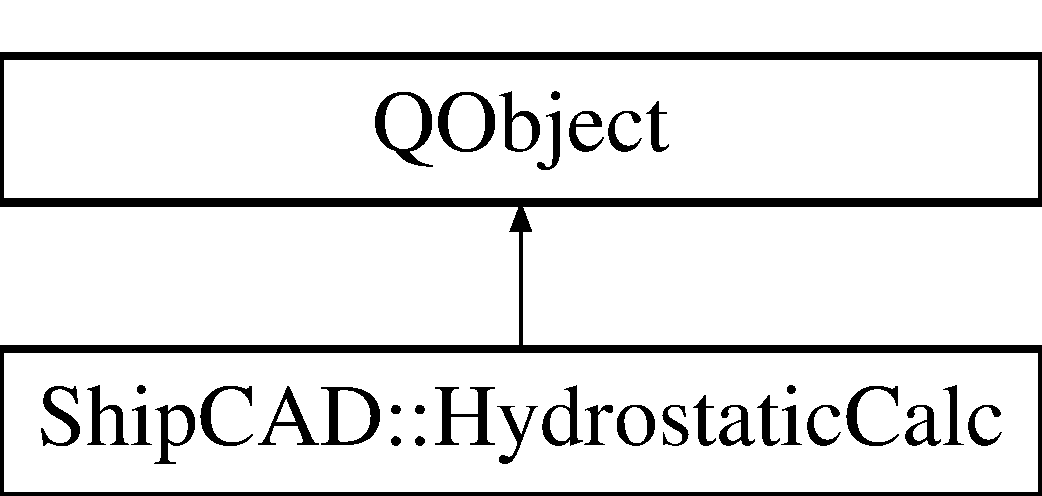
\includegraphics[height=2.000000cm]{classShipCAD_1_1HydrostaticCalc}
\end{center}
\end{figure}
\subsection*{Public Member Functions}
\begin{DoxyCompactItemize}
\item 
\hyperlink{classShipCAD_1_1HydrostaticCalc_a56877acf4c33b3cab96ce381217c7a3b}{Hydrostatic\-Calc} (\hyperlink{classShipCAD_1_1ShipCADModel}{Ship\-C\-A\-D\-Model} $\ast$owner)
\item 
\hyperlink{classShipCAD_1_1HydrostaticCalc_a382835ae6396b82371b605d662fd1696}{$\sim$\-Hydrostatic\-Calc} ()
\item 
void \hyperlink{classShipCAD_1_1HydrostaticCalc_a09403d93ebe095a41b6a29ba9b740b65}{clear} ()
\item 
\hyperlink{classShipCAD_1_1ShipCADModel}{Ship\-C\-A\-D\-Model} $\ast$ \hyperlink{classShipCAD_1_1HydrostaticCalc_ac1dc0e446e711461bb3747326efd8df6}{get\-Owner} () const 
\item 
Q\-String \hyperlink{classShipCAD_1_1HydrostaticCalc_abfc3e3da906e630cf6b763bd3559c630}{get\-Error\-String} () const 
\begin{DoxyCompactList}\small\item\em get the errors with current calculation \end{DoxyCompactList}\item 
\hyperlink{classShipCAD_1_1Plane}{Plane} \hyperlink{classShipCAD_1_1HydrostaticCalc_a157563b0f0258d21a9be615e092d5b21}{get\-Wl\-Plane} () const 
\begin{DoxyCompactList}\small\item\em get the waterline plane (from draft, trim, and heeling angle) \end{DoxyCompactList}\item 
bool \hyperlink{classShipCAD_1_1HydrostaticCalc_a875b9708e91db4a8f06ddbcc8a22d830}{is\-Calculated} ()
\item 
void \hyperlink{classShipCAD_1_1HydrostaticCalc_a0deeafff07f3bb77184df959bbd91266}{set\-Calculated} (bool calc)
\item 
void \hyperlink{classShipCAD_1_1HydrostaticCalc_a6528fe532bbb1121c73972906d108835}{set\-Draft} (float draft)
\item 
\hyperlink{structShipCAD_1_1HydrostaticsData}{Hydrostatics\-Data} \& \hyperlink{classShipCAD_1_1HydrostaticCalc_aabcae04d59358b87b9d5fb4ffda83f1a}{get\-Data} ()
\item 
bool \hyperlink{classShipCAD_1_1HydrostaticCalc_a8ae6f41fd9799cb17a855a9b4f89c5fb}{has\-Error} (\hyperlink{namespaceShipCAD_a1d801b982c24bce0cf10ffd4b995dda0}{hydrostatics\-\_\-error\-\_\-t} error) const 
\begin{DoxyCompactList}\small\item\em does this calculation have this type of error \end{DoxyCompactList}\item 
void \hyperlink{classShipCAD_1_1HydrostaticCalc_ad6415cb7c8e13ded4537292dd3a06688}{add\-Error} (\hyperlink{namespaceShipCAD_a1d801b982c24bce0cf10ffd4b995dda0}{hydrostatics\-\_\-error\-\_\-t} error)
\begin{DoxyCompactList}\small\item\em add this error type to the calculation \end{DoxyCompactList}\item 
bool \hyperlink{classShipCAD_1_1HydrostaticCalc_adb8e8e29d28e2da0e75e30c0636f034b}{has\-Calculation} (\hyperlink{namespaceShipCAD_ac9ff7fc96a52fceafa83edc0d5d06fce}{hydrostatics\-\_\-calc\-\_\-t} ty) const 
\begin{DoxyCompactList}\small\item\em is this type of calculation set \end{DoxyCompactList}\item 
void \hyperlink{classShipCAD_1_1HydrostaticCalc_a32379831790fd88d422c6783b1b70ef7}{add\-Calculation\-Type} (\hyperlink{namespaceShipCAD_ac9ff7fc96a52fceafa83edc0d5d06fce}{hydrostatics\-\_\-calc\-\_\-t} ty)
\begin{DoxyCompactList}\small\item\em set a type of calculation \end{DoxyCompactList}\item 
float \hyperlink{classShipCAD_1_1HydrostaticCalc_a7b27fef68486f663fd325ef316032a03}{get\-Heeling\-Angle} () const 
\begin{DoxyCompactList}\small\item\em get the heeling angle for this calculation \end{DoxyCompactList}\item 
void \hyperlink{classShipCAD_1_1HydrostaticCalc_ae6bf118e2e5e89a8e8d7ea7675fdee22}{set\-Heeling\-Angle} (float angle)
\item 
void \hyperlink{classShipCAD_1_1HydrostaticCalc_a61df8d7421f2900cbc18a6565963c66e}{set\-Hydrostatic\-Type} (\hyperlink{namespaceShipCAD_afea51c7ee52940acebde29bf44206fe2}{hydrostatic\-\_\-type\-\_\-t} ty)
\item 
float \hyperlink{classShipCAD_1_1HydrostaticCalc_aecd19708f7ebadb4321af93565ffc184}{get\-Trim\-Angle} () const 
\begin{DoxyCompactList}\small\item\em get the trim angle for this calculation \end{DoxyCompactList}\item 
void \hyperlink{classShipCAD_1_1HydrostaticCalc_ace579596fa77d8e3ea4f854ca033ed83}{set\-Trim} (float trim)
\begin{DoxyCompactList}\small\item\em set the trim for this calculation (distance, not angle) \end{DoxyCompactList}\item 
void \hyperlink{classShipCAD_1_1HydrostaticCalc_a919bce0b984cbef1c59534d6e9fec46f}{add\-Data} (Q\-String\-List \&strings, \hyperlink{namespaceShipCAD_a2c84d37615dd30be37ed0253501fb9a3}{hydrostatics\-\_\-mode\-\_\-t} mode, Q\-Char separator)
\begin{DoxyCompactList}\small\item\em get all Hydrostatics data in a list of strings \end{DoxyCompactList}\item 
bool \hyperlink{classShipCAD_1_1HydrostaticCalc_a7573a510a6b53e56a79f4042e41ee89e}{balance} (float displacement, bool freetotrim, \hyperlink{structShipCAD_1_1CrosscurvesData}{Crosscurves\-Data} \&output)
\item 
void \hyperlink{classShipCAD_1_1HydrostaticCalc_ab0c8f5dc5c576e6e9eae5fb27fd5bdd0}{calculate} ()
\begin{DoxyCompactList}\small\item\em make all calculations specified \end{DoxyCompactList}\item 
void \hyperlink{classShipCAD_1_1HydrostaticCalc_ad37fd32bf358c96b6653c6c92fd92c20}{calculate\-Volume} (const \hyperlink{classShipCAD_1_1Plane}{Plane} \&waterline\-\_\-plane)
\begin{DoxyCompactList}\small\item\em calculate the volume of the ship below plane \end{DoxyCompactList}\end{DoxyCompactItemize}
\subsection*{Static Public Member Functions}
\begin{DoxyCompactItemize}
\item 
static \hyperlink{classShipCAD_1_1HydrostaticCalc}{Hydrostatic\-Calc} $\ast$ \hyperlink{classShipCAD_1_1HydrostaticCalc_a527c0f0526a159e3d7cb7ddd4925c295}{construct} (\hyperlink{classShipCAD_1_1ShipCADModel}{Ship\-C\-A\-D\-Model} $\ast$owner)
\end{DoxyCompactItemize}
\subsection*{Protected Member Functions}
\begin{DoxyCompactItemize}
\item 
void \hyperlink{classShipCAD_1_1HydrostaticCalc_a95e0e1aa5d11f49cb0f0553ba45af085}{add\-Header} (Q\-String\-List \&strings)
\item 
void \hyperlink{classShipCAD_1_1HydrostaticCalc_aa4077ad7205ef509d3a54edb8e04b8b7}{add\-Footer} (Q\-String\-List \&strings, \hyperlink{namespaceShipCAD_a2c84d37615dd30be37ed0253501fb9a3}{hydrostatics\-\_\-mode\-\_\-t} mode)
\end{DoxyCompactItemize}


\subsection{Detailed Description}
Initialize and execute Hydrostatics Data calculation for a waterplane. 

Definition at line 104 of file hydrostaticcalc.\-h.



\subsection{Constructor \& Destructor Documentation}
\hypertarget{classShipCAD_1_1HydrostaticCalc_a56877acf4c33b3cab96ce381217c7a3b}{\index{Ship\-C\-A\-D\-::\-Hydrostatic\-Calc@{Ship\-C\-A\-D\-::\-Hydrostatic\-Calc}!Hydrostatic\-Calc@{Hydrostatic\-Calc}}
\index{Hydrostatic\-Calc@{Hydrostatic\-Calc}!ShipCAD::HydrostaticCalc@{Ship\-C\-A\-D\-::\-Hydrostatic\-Calc}}
\subsubsection[{Hydrostatic\-Calc}]{\setlength{\rightskip}{0pt plus 5cm}Hydrostatic\-Calc\-::\-Hydrostatic\-Calc (
\begin{DoxyParamCaption}
\item[{{\bf Ship\-C\-A\-D\-Model} $\ast$}]{owner}
\end{DoxyParamCaption}
)\hspace{0.3cm}{\ttfamily [explicit]}}}\label{classShipCAD_1_1HydrostaticCalc_a56877acf4c33b3cab96ce381217c7a3b}


Definition at line 73 of file hydrostaticcalc.\-cpp.

\hypertarget{classShipCAD_1_1HydrostaticCalc_a382835ae6396b82371b605d662fd1696}{\index{Ship\-C\-A\-D\-::\-Hydrostatic\-Calc@{Ship\-C\-A\-D\-::\-Hydrostatic\-Calc}!$\sim$\-Hydrostatic\-Calc@{$\sim$\-Hydrostatic\-Calc}}
\index{$\sim$\-Hydrostatic\-Calc@{$\sim$\-Hydrostatic\-Calc}!ShipCAD::HydrostaticCalc@{Ship\-C\-A\-D\-::\-Hydrostatic\-Calc}}
\subsubsection[{$\sim$\-Hydrostatic\-Calc}]{\setlength{\rightskip}{0pt plus 5cm}Hydrostatic\-Calc\-::$\sim$\-Hydrostatic\-Calc (
\begin{DoxyParamCaption}
{}
\end{DoxyParamCaption}
)}}\label{classShipCAD_1_1HydrostaticCalc_a382835ae6396b82371b605d662fd1696}


Definition at line 81 of file hydrostaticcalc.\-cpp.



\subsection{Member Function Documentation}
\hypertarget{classShipCAD_1_1HydrostaticCalc_a32379831790fd88d422c6783b1b70ef7}{\index{Ship\-C\-A\-D\-::\-Hydrostatic\-Calc@{Ship\-C\-A\-D\-::\-Hydrostatic\-Calc}!add\-Calculation\-Type@{add\-Calculation\-Type}}
\index{add\-Calculation\-Type@{add\-Calculation\-Type}!ShipCAD::HydrostaticCalc@{Ship\-C\-A\-D\-::\-Hydrostatic\-Calc}}
\subsubsection[{add\-Calculation\-Type}]{\setlength{\rightskip}{0pt plus 5cm}void Ship\-C\-A\-D\-::\-Hydrostatic\-Calc\-::add\-Calculation\-Type (
\begin{DoxyParamCaption}
\item[{{\bf hydrostatics\-\_\-calc\-\_\-t}}]{ty}
\end{DoxyParamCaption}
)\hspace{0.3cm}{\ttfamily [inline]}}}\label{classShipCAD_1_1HydrostaticCalc_a32379831790fd88d422c6783b1b70ef7}


set a type of calculation 


\begin{DoxyParams}{Parameters}
{\em ty} & type of calculation to add to set \\
\hline
\end{DoxyParams}


Definition at line 153 of file hydrostaticcalc.\-h.

\hypertarget{classShipCAD_1_1HydrostaticCalc_a919bce0b984cbef1c59534d6e9fec46f}{\index{Ship\-C\-A\-D\-::\-Hydrostatic\-Calc@{Ship\-C\-A\-D\-::\-Hydrostatic\-Calc}!add\-Data@{add\-Data}}
\index{add\-Data@{add\-Data}!ShipCAD::HydrostaticCalc@{Ship\-C\-A\-D\-::\-Hydrostatic\-Calc}}
\subsubsection[{add\-Data}]{\setlength{\rightskip}{0pt plus 5cm}void Hydrostatic\-Calc\-::add\-Data (
\begin{DoxyParamCaption}
\item[{Q\-String\-List \&}]{strings, }
\item[{{\bf hydrostatics\-\_\-mode\-\_\-t}}]{mode, }
\item[{Q\-Char}]{separator}
\end{DoxyParamCaption}
)}}\label{classShipCAD_1_1HydrostaticCalc_a919bce0b984cbef1c59534d6e9fec46f}


get all Hydrostatics data in a list of strings 


\begin{DoxyParams}{Parameters}
{\em strings} & target string list for data \\
\hline
{\em mode} & how to display the data \\
\hline
{\em separator} & character to separate the data \\
\hline
\end{DoxyParams}


Definition at line 189 of file hydrostaticcalc.\-cpp.

\hypertarget{classShipCAD_1_1HydrostaticCalc_ad6415cb7c8e13ded4537292dd3a06688}{\index{Ship\-C\-A\-D\-::\-Hydrostatic\-Calc@{Ship\-C\-A\-D\-::\-Hydrostatic\-Calc}!add\-Error@{add\-Error}}
\index{add\-Error@{add\-Error}!ShipCAD::HydrostaticCalc@{Ship\-C\-A\-D\-::\-Hydrostatic\-Calc}}
\subsubsection[{add\-Error}]{\setlength{\rightskip}{0pt plus 5cm}void Ship\-C\-A\-D\-::\-Hydrostatic\-Calc\-::add\-Error (
\begin{DoxyParamCaption}
\item[{{\bf hydrostatics\-\_\-error\-\_\-t}}]{error}
\end{DoxyParamCaption}
)\hspace{0.3cm}{\ttfamily [inline]}}}\label{classShipCAD_1_1HydrostaticCalc_ad6415cb7c8e13ded4537292dd3a06688}


add this error type to the calculation 


\begin{DoxyParams}{Parameters}
{\em error} & the error to add \\
\hline
\end{DoxyParams}


Definition at line 142 of file hydrostaticcalc.\-h.

\hypertarget{classShipCAD_1_1HydrostaticCalc_aa4077ad7205ef509d3a54edb8e04b8b7}{\index{Ship\-C\-A\-D\-::\-Hydrostatic\-Calc@{Ship\-C\-A\-D\-::\-Hydrostatic\-Calc}!add\-Footer@{add\-Footer}}
\index{add\-Footer@{add\-Footer}!ShipCAD::HydrostaticCalc@{Ship\-C\-A\-D\-::\-Hydrostatic\-Calc}}
\subsubsection[{add\-Footer}]{\setlength{\rightskip}{0pt plus 5cm}void Hydrostatic\-Calc\-::add\-Footer (
\begin{DoxyParamCaption}
\item[{Q\-String\-List \&}]{strings, }
\item[{{\bf hydrostatics\-\_\-mode\-\_\-t}}]{mode}
\end{DoxyParamCaption}
)\hspace{0.3cm}{\ttfamily [protected]}}}\label{classShipCAD_1_1HydrostaticCalc_aa4077ad7205ef509d3a54edb8e04b8b7}


Definition at line 390 of file hydrostaticcalc.\-cpp.

\hypertarget{classShipCAD_1_1HydrostaticCalc_a95e0e1aa5d11f49cb0f0553ba45af085}{\index{Ship\-C\-A\-D\-::\-Hydrostatic\-Calc@{Ship\-C\-A\-D\-::\-Hydrostatic\-Calc}!add\-Header@{add\-Header}}
\index{add\-Header@{add\-Header}!ShipCAD::HydrostaticCalc@{Ship\-C\-A\-D\-::\-Hydrostatic\-Calc}}
\subsubsection[{add\-Header}]{\setlength{\rightskip}{0pt plus 5cm}void Hydrostatic\-Calc\-::add\-Header (
\begin{DoxyParamCaption}
\item[{Q\-String\-List \&}]{strings}
\end{DoxyParamCaption}
)\hspace{0.3cm}{\ttfamily [protected]}}}\label{classShipCAD_1_1HydrostaticCalc_a95e0e1aa5d11f49cb0f0553ba45af085}


Definition at line 349 of file hydrostaticcalc.\-cpp.

\hypertarget{classShipCAD_1_1HydrostaticCalc_a7573a510a6b53e56a79f4042e41ee89e}{\index{Ship\-C\-A\-D\-::\-Hydrostatic\-Calc@{Ship\-C\-A\-D\-::\-Hydrostatic\-Calc}!balance@{balance}}
\index{balance@{balance}!ShipCAD::HydrostaticCalc@{Ship\-C\-A\-D\-::\-Hydrostatic\-Calc}}
\subsubsection[{balance}]{\setlength{\rightskip}{0pt plus 5cm}bool Hydrostatic\-Calc\-::balance (
\begin{DoxyParamCaption}
\item[{float}]{displacement, }
\item[{bool}]{freetotrim, }
\item[{{\bf Crosscurves\-Data} \&}]{output}
\end{DoxyParamCaption}
)}}\label{classShipCAD_1_1HydrostaticCalc_a7573a510a6b53e56a79f4042e41ee89e}


Definition at line 577 of file hydrostaticcalc.\-cpp.

\hypertarget{classShipCAD_1_1HydrostaticCalc_ab0c8f5dc5c576e6e9eae5fb27fd5bdd0}{\index{Ship\-C\-A\-D\-::\-Hydrostatic\-Calc@{Ship\-C\-A\-D\-::\-Hydrostatic\-Calc}!calculate@{calculate}}
\index{calculate@{calculate}!ShipCAD::HydrostaticCalc@{Ship\-C\-A\-D\-::\-Hydrostatic\-Calc}}
\subsubsection[{calculate}]{\setlength{\rightskip}{0pt plus 5cm}void Hydrostatic\-Calc\-::calculate (
\begin{DoxyParamCaption}
{}
\end{DoxyParamCaption}
)}}\label{classShipCAD_1_1HydrostaticCalc_ab0c8f5dc5c576e6e9eae5fb27fd5bdd0}


make all calculations specified 

For each type of calculation specified, this method will fill out \-\_\-data with the results of that calculation The calculated flag will also be set 

Definition at line 918 of file hydrostaticcalc.\-cpp.

\hypertarget{classShipCAD_1_1HydrostaticCalc_ad37fd32bf358c96b6653c6c92fd92c20}{\index{Ship\-C\-A\-D\-::\-Hydrostatic\-Calc@{Ship\-C\-A\-D\-::\-Hydrostatic\-Calc}!calculate\-Volume@{calculate\-Volume}}
\index{calculate\-Volume@{calculate\-Volume}!ShipCAD::HydrostaticCalc@{Ship\-C\-A\-D\-::\-Hydrostatic\-Calc}}
\subsubsection[{calculate\-Volume}]{\setlength{\rightskip}{0pt plus 5cm}void Hydrostatic\-Calc\-::calculate\-Volume (
\begin{DoxyParamCaption}
\item[{const {\bf Plane} \&}]{waterline\-\_\-plane}
\end{DoxyParamCaption}
)}}\label{classShipCAD_1_1HydrostaticCalc_ad37fd32bf358c96b6653c6c92fd92c20}


calculate the volume of the ship below plane 

When this method is completed, then \-\_\-data will have absolute\-\_\-draft, errors, leak point, center\-\_\-of\-\_\-buoyancy, lcb\-\_\-perc, length\-\_\-waterline, width\-\_\-waterline, displacement, volume calculated The calculated flag will also be set


\begin{DoxyParams}{Parameters}
{\em waterline\-\_\-plane} & the plane of the waterline \\
\hline
\end{DoxyParams}


Definition at line 1052 of file hydrostaticcalc.\-cpp.

\hypertarget{classShipCAD_1_1HydrostaticCalc_a09403d93ebe095a41b6a29ba9b740b65}{\index{Ship\-C\-A\-D\-::\-Hydrostatic\-Calc@{Ship\-C\-A\-D\-::\-Hydrostatic\-Calc}!clear@{clear}}
\index{clear@{clear}!ShipCAD::HydrostaticCalc@{Ship\-C\-A\-D\-::\-Hydrostatic\-Calc}}
\subsubsection[{clear}]{\setlength{\rightskip}{0pt plus 5cm}void Hydrostatic\-Calc\-::clear (
\begin{DoxyParamCaption}
{}
\end{DoxyParamCaption}
)}}\label{classShipCAD_1_1HydrostaticCalc_a09403d93ebe095a41b6a29ba9b740b65}


Definition at line 92 of file hydrostaticcalc.\-cpp.

\hypertarget{classShipCAD_1_1HydrostaticCalc_a527c0f0526a159e3d7cb7ddd4925c295}{\index{Ship\-C\-A\-D\-::\-Hydrostatic\-Calc@{Ship\-C\-A\-D\-::\-Hydrostatic\-Calc}!construct@{construct}}
\index{construct@{construct}!ShipCAD::HydrostaticCalc@{Ship\-C\-A\-D\-::\-Hydrostatic\-Calc}}
\subsubsection[{construct}]{\setlength{\rightskip}{0pt plus 5cm}{\bf Hydrostatic\-Calc} $\ast$ Hydrostatic\-Calc\-::construct (
\begin{DoxyParamCaption}
\item[{{\bf Ship\-C\-A\-D\-Model} $\ast$}]{owner}
\end{DoxyParamCaption}
)\hspace{0.3cm}{\ttfamily [static]}}}\label{classShipCAD_1_1HydrostaticCalc_a527c0f0526a159e3d7cb7ddd4925c295}


Definition at line 86 of file hydrostaticcalc.\-cpp.

\hypertarget{classShipCAD_1_1HydrostaticCalc_aabcae04d59358b87b9d5fb4ffda83f1a}{\index{Ship\-C\-A\-D\-::\-Hydrostatic\-Calc@{Ship\-C\-A\-D\-::\-Hydrostatic\-Calc}!get\-Data@{get\-Data}}
\index{get\-Data@{get\-Data}!ShipCAD::HydrostaticCalc@{Ship\-C\-A\-D\-::\-Hydrostatic\-Calc}}
\subsubsection[{get\-Data}]{\setlength{\rightskip}{0pt plus 5cm}{\bf Hydrostatics\-Data}\& Ship\-C\-A\-D\-::\-Hydrostatic\-Calc\-::get\-Data (
\begin{DoxyParamCaption}
{}
\end{DoxyParamCaption}
)\hspace{0.3cm}{\ttfamily [inline]}}}\label{classShipCAD_1_1HydrostaticCalc_aabcae04d59358b87b9d5fb4ffda83f1a}


Definition at line 131 of file hydrostaticcalc.\-h.

\hypertarget{classShipCAD_1_1HydrostaticCalc_abfc3e3da906e630cf6b763bd3559c630}{\index{Ship\-C\-A\-D\-::\-Hydrostatic\-Calc@{Ship\-C\-A\-D\-::\-Hydrostatic\-Calc}!get\-Error\-String@{get\-Error\-String}}
\index{get\-Error\-String@{get\-Error\-String}!ShipCAD::HydrostaticCalc@{Ship\-C\-A\-D\-::\-Hydrostatic\-Calc}}
\subsubsection[{get\-Error\-String}]{\setlength{\rightskip}{0pt plus 5cm}Q\-String Hydrostatic\-Calc\-::get\-Error\-String (
\begin{DoxyParamCaption}
{}
\end{DoxyParamCaption}
) const}}\label{classShipCAD_1_1HydrostaticCalc_abfc3e3da906e630cf6b763bd3559c630}


get the errors with current calculation 

\begin{DoxyReturn}{Returns}
string with current errors 
\end{DoxyReturn}


Definition at line 104 of file hydrostaticcalc.\-cpp.

\hypertarget{classShipCAD_1_1HydrostaticCalc_a7b27fef68486f663fd325ef316032a03}{\index{Ship\-C\-A\-D\-::\-Hydrostatic\-Calc@{Ship\-C\-A\-D\-::\-Hydrostatic\-Calc}!get\-Heeling\-Angle@{get\-Heeling\-Angle}}
\index{get\-Heeling\-Angle@{get\-Heeling\-Angle}!ShipCAD::HydrostaticCalc@{Ship\-C\-A\-D\-::\-Hydrostatic\-Calc}}
\subsubsection[{get\-Heeling\-Angle}]{\setlength{\rightskip}{0pt plus 5cm}float Ship\-C\-A\-D\-::\-Hydrostatic\-Calc\-::get\-Heeling\-Angle (
\begin{DoxyParamCaption}
{}
\end{DoxyParamCaption}
) const\hspace{0.3cm}{\ttfamily [inline]}}}\label{classShipCAD_1_1HydrostaticCalc_a7b27fef68486f663fd325ef316032a03}


get the heeling angle for this calculation 

\begin{DoxyReturn}{Returns}
the heeling angle in degrees 
\end{DoxyReturn}


Definition at line 159 of file hydrostaticcalc.\-h.

\hypertarget{classShipCAD_1_1HydrostaticCalc_ac1dc0e446e711461bb3747326efd8df6}{\index{Ship\-C\-A\-D\-::\-Hydrostatic\-Calc@{Ship\-C\-A\-D\-::\-Hydrostatic\-Calc}!get\-Owner@{get\-Owner}}
\index{get\-Owner@{get\-Owner}!ShipCAD::HydrostaticCalc@{Ship\-C\-A\-D\-::\-Hydrostatic\-Calc}}
\subsubsection[{get\-Owner}]{\setlength{\rightskip}{0pt plus 5cm}{\bf Ship\-C\-A\-D\-Model}$\ast$ Ship\-C\-A\-D\-::\-Hydrostatic\-Calc\-::get\-Owner (
\begin{DoxyParamCaption}
{}
\end{DoxyParamCaption}
) const\hspace{0.3cm}{\ttfamily [inline]}}}\label{classShipCAD_1_1HydrostaticCalc_ac1dc0e446e711461bb3747326efd8df6}


Definition at line 116 of file hydrostaticcalc.\-h.

\hypertarget{classShipCAD_1_1HydrostaticCalc_aecd19708f7ebadb4321af93565ffc184}{\index{Ship\-C\-A\-D\-::\-Hydrostatic\-Calc@{Ship\-C\-A\-D\-::\-Hydrostatic\-Calc}!get\-Trim\-Angle@{get\-Trim\-Angle}}
\index{get\-Trim\-Angle@{get\-Trim\-Angle}!ShipCAD::HydrostaticCalc@{Ship\-C\-A\-D\-::\-Hydrostatic\-Calc}}
\subsubsection[{get\-Trim\-Angle}]{\setlength{\rightskip}{0pt plus 5cm}float Hydrostatic\-Calc\-::get\-Trim\-Angle (
\begin{DoxyParamCaption}
{}
\end{DoxyParamCaption}
) const}}\label{classShipCAD_1_1HydrostaticCalc_aecd19708f7ebadb4321af93565ffc184}


get the trim angle for this calculation 

The trim angle is calculated from the given trim and waterline plane.

\begin{DoxyReturn}{Returns}
the angle of trim in degrees 
\end{DoxyReturn}


Definition at line 118 of file hydrostaticcalc.\-cpp.

\hypertarget{classShipCAD_1_1HydrostaticCalc_a157563b0f0258d21a9be615e092d5b21}{\index{Ship\-C\-A\-D\-::\-Hydrostatic\-Calc@{Ship\-C\-A\-D\-::\-Hydrostatic\-Calc}!get\-Wl\-Plane@{get\-Wl\-Plane}}
\index{get\-Wl\-Plane@{get\-Wl\-Plane}!ShipCAD::HydrostaticCalc@{Ship\-C\-A\-D\-::\-Hydrostatic\-Calc}}
\subsubsection[{get\-Wl\-Plane}]{\setlength{\rightskip}{0pt plus 5cm}{\bf Plane} Hydrostatic\-Calc\-::get\-Wl\-Plane (
\begin{DoxyParamCaption}
{}
\end{DoxyParamCaption}
) const}}\label{classShipCAD_1_1HydrostaticCalc_a157563b0f0258d21a9be615e092d5b21}


get the waterline plane (from draft, trim, and heeling angle) 

\begin{DoxyReturn}{Returns}
the waterline plane 
\end{DoxyReturn}


Definition at line 125 of file hydrostaticcalc.\-cpp.

\hypertarget{classShipCAD_1_1HydrostaticCalc_adb8e8e29d28e2da0e75e30c0636f034b}{\index{Ship\-C\-A\-D\-::\-Hydrostatic\-Calc@{Ship\-C\-A\-D\-::\-Hydrostatic\-Calc}!has\-Calculation@{has\-Calculation}}
\index{has\-Calculation@{has\-Calculation}!ShipCAD::HydrostaticCalc@{Ship\-C\-A\-D\-::\-Hydrostatic\-Calc}}
\subsubsection[{has\-Calculation}]{\setlength{\rightskip}{0pt plus 5cm}bool Hydrostatic\-Calc\-::has\-Calculation (
\begin{DoxyParamCaption}
\item[{{\bf hydrostatics\-\_\-calc\-\_\-t}}]{ty}
\end{DoxyParamCaption}
) const}}\label{classShipCAD_1_1HydrostaticCalc_adb8e8e29d28e2da0e75e30c0636f034b}


is this type of calculation set 


\begin{DoxyParams}{Parameters}
{\em ty} & type of calculation to check for \\
\hline
\end{DoxyParams}
\begin{DoxyReturn}{Returns}
true if type is part of set 
\end{DoxyReturn}


Definition at line 184 of file hydrostaticcalc.\-cpp.

\hypertarget{classShipCAD_1_1HydrostaticCalc_a8ae6f41fd9799cb17a855a9b4f89c5fb}{\index{Ship\-C\-A\-D\-::\-Hydrostatic\-Calc@{Ship\-C\-A\-D\-::\-Hydrostatic\-Calc}!has\-Error@{has\-Error}}
\index{has\-Error@{has\-Error}!ShipCAD::HydrostaticCalc@{Ship\-C\-A\-D\-::\-Hydrostatic\-Calc}}
\subsubsection[{has\-Error}]{\setlength{\rightskip}{0pt plus 5cm}bool Hydrostatic\-Calc\-::has\-Error (
\begin{DoxyParamCaption}
\item[{{\bf hydrostatics\-\_\-error\-\_\-t}}]{error}
\end{DoxyParamCaption}
) const}}\label{classShipCAD_1_1HydrostaticCalc_a8ae6f41fd9799cb17a855a9b4f89c5fb}


does this calculation have this type of error 


\begin{DoxyParams}{Parameters}
{\em error} & the error to check for \\
\hline
\end{DoxyParams}
\begin{DoxyReturn}{Returns}
true if calculation has this error 
\end{DoxyReturn}


Definition at line 179 of file hydrostaticcalc.\-cpp.

\hypertarget{classShipCAD_1_1HydrostaticCalc_a875b9708e91db4a8f06ddbcc8a22d830}{\index{Ship\-C\-A\-D\-::\-Hydrostatic\-Calc@{Ship\-C\-A\-D\-::\-Hydrostatic\-Calc}!is\-Calculated@{is\-Calculated}}
\index{is\-Calculated@{is\-Calculated}!ShipCAD::HydrostaticCalc@{Ship\-C\-A\-D\-::\-Hydrostatic\-Calc}}
\subsubsection[{is\-Calculated}]{\setlength{\rightskip}{0pt plus 5cm}bool Ship\-C\-A\-D\-::\-Hydrostatic\-Calc\-::is\-Calculated (
\begin{DoxyParamCaption}
{}
\end{DoxyParamCaption}
)\hspace{0.3cm}{\ttfamily [inline]}}}\label{classShipCAD_1_1HydrostaticCalc_a875b9708e91db4a8f06ddbcc8a22d830}


Definition at line 128 of file hydrostaticcalc.\-h.

\hypertarget{classShipCAD_1_1HydrostaticCalc_a0deeafff07f3bb77184df959bbd91266}{\index{Ship\-C\-A\-D\-::\-Hydrostatic\-Calc@{Ship\-C\-A\-D\-::\-Hydrostatic\-Calc}!set\-Calculated@{set\-Calculated}}
\index{set\-Calculated@{set\-Calculated}!ShipCAD::HydrostaticCalc@{Ship\-C\-A\-D\-::\-Hydrostatic\-Calc}}
\subsubsection[{set\-Calculated}]{\setlength{\rightskip}{0pt plus 5cm}void Hydrostatic\-Calc\-::set\-Calculated (
\begin{DoxyParamCaption}
\item[{bool}]{calc}
\end{DoxyParamCaption}
)}}\label{classShipCAD_1_1HydrostaticCalc_a0deeafff07f3bb77184df959bbd91266}


Definition at line 137 of file hydrostaticcalc.\-cpp.

\hypertarget{classShipCAD_1_1HydrostaticCalc_a6528fe532bbb1121c73972906d108835}{\index{Ship\-C\-A\-D\-::\-Hydrostatic\-Calc@{Ship\-C\-A\-D\-::\-Hydrostatic\-Calc}!set\-Draft@{set\-Draft}}
\index{set\-Draft@{set\-Draft}!ShipCAD::HydrostaticCalc@{Ship\-C\-A\-D\-::\-Hydrostatic\-Calc}}
\subsubsection[{set\-Draft}]{\setlength{\rightskip}{0pt plus 5cm}void Hydrostatic\-Calc\-::set\-Draft (
\begin{DoxyParamCaption}
\item[{float}]{draft}
\end{DoxyParamCaption}
)}}\label{classShipCAD_1_1HydrostaticCalc_a6528fe532bbb1121c73972906d108835}


Definition at line 147 of file hydrostaticcalc.\-cpp.

\hypertarget{classShipCAD_1_1HydrostaticCalc_ae6bf118e2e5e89a8e8d7ea7675fdee22}{\index{Ship\-C\-A\-D\-::\-Hydrostatic\-Calc@{Ship\-C\-A\-D\-::\-Hydrostatic\-Calc}!set\-Heeling\-Angle@{set\-Heeling\-Angle}}
\index{set\-Heeling\-Angle@{set\-Heeling\-Angle}!ShipCAD::HydrostaticCalc@{Ship\-C\-A\-D\-::\-Hydrostatic\-Calc}}
\subsubsection[{set\-Heeling\-Angle}]{\setlength{\rightskip}{0pt plus 5cm}void Hydrostatic\-Calc\-::set\-Heeling\-Angle (
\begin{DoxyParamCaption}
\item[{float}]{angle}
\end{DoxyParamCaption}
)}}\label{classShipCAD_1_1HydrostaticCalc_ae6bf118e2e5e89a8e8d7ea7675fdee22}


Definition at line 155 of file hydrostaticcalc.\-cpp.

\hypertarget{classShipCAD_1_1HydrostaticCalc_a61df8d7421f2900cbc18a6565963c66e}{\index{Ship\-C\-A\-D\-::\-Hydrostatic\-Calc@{Ship\-C\-A\-D\-::\-Hydrostatic\-Calc}!set\-Hydrostatic\-Type@{set\-Hydrostatic\-Type}}
\index{set\-Hydrostatic\-Type@{set\-Hydrostatic\-Type}!ShipCAD::HydrostaticCalc@{Ship\-C\-A\-D\-::\-Hydrostatic\-Calc}}
\subsubsection[{set\-Hydrostatic\-Type}]{\setlength{\rightskip}{0pt plus 5cm}void Hydrostatic\-Calc\-::set\-Hydrostatic\-Type (
\begin{DoxyParamCaption}
\item[{{\bf hydrostatic\-\_\-type\-\_\-t}}]{ty}
\end{DoxyParamCaption}
)}}\label{classShipCAD_1_1HydrostaticCalc_a61df8d7421f2900cbc18a6565963c66e}


Definition at line 163 of file hydrostaticcalc.\-cpp.

\hypertarget{classShipCAD_1_1HydrostaticCalc_ace579596fa77d8e3ea4f854ca033ed83}{\index{Ship\-C\-A\-D\-::\-Hydrostatic\-Calc@{Ship\-C\-A\-D\-::\-Hydrostatic\-Calc}!set\-Trim@{set\-Trim}}
\index{set\-Trim@{set\-Trim}!ShipCAD::HydrostaticCalc@{Ship\-C\-A\-D\-::\-Hydrostatic\-Calc}}
\subsubsection[{set\-Trim}]{\setlength{\rightskip}{0pt plus 5cm}void Hydrostatic\-Calc\-::set\-Trim (
\begin{DoxyParamCaption}
\item[{float}]{trim}
\end{DoxyParamCaption}
)}}\label{classShipCAD_1_1HydrostaticCalc_ace579596fa77d8e3ea4f854ca033ed83}


set the trim for this calculation (distance, not angle) 


\begin{DoxyParams}{Parameters}
{\em trim} & the trim of the hull \\
\hline
\end{DoxyParams}


Definition at line 171 of file hydrostaticcalc.\-cpp.



The documentation for this class was generated from the following files\-:\begin{DoxyCompactItemize}
\item 
Ship\-C\-A\-Dlib/\hyperlink{hydrostaticcalc_8h}{hydrostaticcalc.\-h}\item 
Ship\-C\-A\-Dlib/\hyperlink{hydrostaticcalc_8cpp}{hydrostaticcalc.\-cpp}\end{DoxyCompactItemize}

\hypertarget{structShipCAD_1_1HydrostaticsData}{\section{Ship\-C\-A\-D\-:\-:Hydrostatics\-Data Struct Reference}
\label{structShipCAD_1_1HydrostaticsData}\index{Ship\-C\-A\-D\-::\-Hydrostatics\-Data@{Ship\-C\-A\-D\-::\-Hydrostatics\-Data}}
}


Structure to hold Hydrostatics Calculation results.  




{\ttfamily \#include $<$hydrostaticcalc.\-h$>$}

\subsection*{Public Member Functions}
\begin{DoxyCompactItemize}
\item 
void \hyperlink{structShipCAD_1_1HydrostaticsData_a7ea81ac589a3b24424b4176c734c7a37}{clear} ()
\begin{DoxyCompactList}\small\item\em reset all data to default values \end{DoxyCompactList}\end{DoxyCompactItemize}
\subsection*{Public Attributes}
\begin{DoxyCompactItemize}
\item 
Q\-Vector3\-D \hyperlink{structShipCAD_1_1HydrostaticsData_acd93669bc08fa097974d41fbaf4dc81f}{model\-\_\-min}
\item 
Q\-Vector3\-D \hyperlink{structShipCAD_1_1HydrostaticsData_a9319fb2ad054a595b6e3b3fd4059a3ae}{model\-\_\-max}
\item 
Q\-Vector3\-D \hyperlink{structShipCAD_1_1HydrostaticsData_a3bb2750b6306d9e8ae09bb4eebb1ed0c}{wl\-\_\-min}
\item 
Q\-Vector3\-D \hyperlink{structShipCAD_1_1HydrostaticsData_a332be807e8373521c238d82b9dcedc38}{wl\-\_\-max}
\item 
Q\-Vector3\-D \hyperlink{structShipCAD_1_1HydrostaticsData_a2d0a1e5f6bf98f8eceb958e5f7e7c73e}{sub\-\_\-min}
\item 
Q\-Vector3\-D \hyperlink{structShipCAD_1_1HydrostaticsData_ab3a6e316a991426c74673025439f123c}{sub\-\_\-max}
\item 
\hyperlink{classShipCAD_1_1Plane}{Plane} \hyperlink{structShipCAD_1_1HydrostaticsData_af93141f846f6622bb146cda042962303}{waterline\-\_\-plane}
\item 
float \hyperlink{structShipCAD_1_1HydrostaticsData_a6857139c04212164c5557cc816f80345}{absolute\-\_\-draft}
\item 
float \hyperlink{structShipCAD_1_1HydrostaticsData_acfbee81bded1b067a23cfc8cc9c00855}{volume}
\item 
float \hyperlink{structShipCAD_1_1HydrostaticsData_a92d1a8a97eb9b21bad485e40ac4461a0}{displacement}
\item 
Q\-Vector3\-D \hyperlink{structShipCAD_1_1HydrostaticsData_a316b31598f53f036c7008cc4910293f8}{center\-\_\-of\-\_\-buoyancy}
\item 
float \hyperlink{structShipCAD_1_1HydrostaticsData_a783b71d811732bbc002b52f21d63c83a}{lcb\-\_\-perc}
\item 
float \hyperlink{structShipCAD_1_1HydrostaticsData_ae65aa54bcbfb059f11aa174cfaa0447b}{length\-\_\-waterline}
\item 
float \hyperlink{structShipCAD_1_1HydrostaticsData_ab79755f5814572be0dfd3ae3ba214fca}{beam\-\_\-waterline}
\item 
float \hyperlink{structShipCAD_1_1HydrostaticsData_ac59c717b9869f0aacca4305fd81d4882}{block\-\_\-coefficient}
\item 
float \hyperlink{structShipCAD_1_1HydrostaticsData_ad4b78176732ea80000adb94b5b5669f3}{wetted\-\_\-surface}
\item 
Q\-Vector3\-D \hyperlink{structShipCAD_1_1HydrostaticsData_a1132babc4274499418c2dc8ea6f86314}{leak}
\item 
float \hyperlink{structShipCAD_1_1HydrostaticsData_ab2b49d5dea89ae998116c8ff4cac2b53}{mainframe\-\_\-area}
\item 
Q\-Vector3\-D \hyperlink{structShipCAD_1_1HydrostaticsData_ab726ebe5c185d197a25e4477576266a4}{mainframe\-\_\-cog}
\item 
float \hyperlink{structShipCAD_1_1HydrostaticsData_a4208b97fe6110516d71e67708186897a}{mainframe\-\_\-coeff}
\item 
float \hyperlink{structShipCAD_1_1HydrostaticsData_a5f3432f4d790bbb9c4d75502cb15b7f0}{waterplane\-\_\-area}
\item 
Q\-Vector3\-D \hyperlink{structShipCAD_1_1HydrostaticsData_ac100876d13ae75147585c5c0f80801fe}{waterplane\-\_\-cog}
\item 
float \hyperlink{structShipCAD_1_1HydrostaticsData_a3e22cf4f03f02a3c0d14e7f66610fd80}{waterplane\-\_\-entrance\-\_\-angle}
\item 
float \hyperlink{structShipCAD_1_1HydrostaticsData_a4d5eb630367999a611b95dd0d2c2242c}{waterplane\-\_\-coeff}
\item 
Q\-Vector2\-D \hyperlink{structShipCAD_1_1HydrostaticsData_a2a662521564e9c0160c15acf9d3121f9}{waterplane\-\_\-mom\-\_\-inertia}
\item 
float \hyperlink{structShipCAD_1_1HydrostaticsData_adbadaf4eafa63f1f10778f4c3e1f61a4}{km\-\_\-transverse}
\item 
float \hyperlink{structShipCAD_1_1HydrostaticsData_a0a51e62f7d169fa892eaabc6a1937256}{km\-\_\-longitudinal}
\item 
float \hyperlink{structShipCAD_1_1HydrostaticsData_a1ba65b28e4351a4d97bc64cd11ddab90}{lateral\-\_\-area}
\item 
Q\-Vector3\-D \hyperlink{structShipCAD_1_1HydrostaticsData_adc0c4f2f0c5b110a968e45642dc5eeeb}{lateral\-\_\-cog}
\item 
float \hyperlink{structShipCAD_1_1HydrostaticsData_acabee310fcde293fcb0d9a5fd5effe27}{prism\-\_\-coefficient}
\item 
float \hyperlink{structShipCAD_1_1HydrostaticsData_a2a7fc6a194bc1e78ecce8ab16512d1eb}{vert\-\_\-prism\-\_\-coefficient}
\item 
std\-::vector$<$ Q\-Vector2\-D $>$ \hyperlink{structShipCAD_1_1HydrostaticsData_a503a1f2299db9d5ae923e598b8ee31ba}{sac}
\end{DoxyCompactItemize}


\subsection{Detailed Description}
Structure to hold Hydrostatics Calculation results. 

Definition at line 50 of file hydrostaticcalc.\-h.



\subsection{Member Function Documentation}
\hypertarget{structShipCAD_1_1HydrostaticsData_a7ea81ac589a3b24424b4176c734c7a37}{\index{Ship\-C\-A\-D\-::\-Hydrostatics\-Data@{Ship\-C\-A\-D\-::\-Hydrostatics\-Data}!clear@{clear}}
\index{clear@{clear}!ShipCAD::HydrostaticsData@{Ship\-C\-A\-D\-::\-Hydrostatics\-Data}}
\subsubsection[{clear}]{\setlength{\rightskip}{0pt plus 5cm}void Hydrostatics\-Data\-::clear (
\begin{DoxyParamCaption}
{}
\end{DoxyParamCaption}
)}}\label{structShipCAD_1_1HydrostaticsData_a7ea81ac589a3b24424b4176c734c7a37}


reset all data to default values 



Definition at line 45 of file hydrostaticcalc.\-cpp.



\subsection{Member Data Documentation}
\hypertarget{structShipCAD_1_1HydrostaticsData_a6857139c04212164c5557cc816f80345}{\index{Ship\-C\-A\-D\-::\-Hydrostatics\-Data@{Ship\-C\-A\-D\-::\-Hydrostatics\-Data}!absolute\-\_\-draft@{absolute\-\_\-draft}}
\index{absolute\-\_\-draft@{absolute\-\_\-draft}!ShipCAD::HydrostaticsData@{Ship\-C\-A\-D\-::\-Hydrostatics\-Data}}
\subsubsection[{absolute\-\_\-draft}]{\setlength{\rightskip}{0pt plus 5cm}float Ship\-C\-A\-D\-::\-Hydrostatics\-Data\-::absolute\-\_\-draft}}\label{structShipCAD_1_1HydrostaticsData_a6857139c04212164c5557cc816f80345}


Definition at line 59 of file hydrostaticcalc.\-h.

\hypertarget{structShipCAD_1_1HydrostaticsData_ab79755f5814572be0dfd3ae3ba214fca}{\index{Ship\-C\-A\-D\-::\-Hydrostatics\-Data@{Ship\-C\-A\-D\-::\-Hydrostatics\-Data}!beam\-\_\-waterline@{beam\-\_\-waterline}}
\index{beam\-\_\-waterline@{beam\-\_\-waterline}!ShipCAD::HydrostaticsData@{Ship\-C\-A\-D\-::\-Hydrostatics\-Data}}
\subsubsection[{beam\-\_\-waterline}]{\setlength{\rightskip}{0pt plus 5cm}float Ship\-C\-A\-D\-::\-Hydrostatics\-Data\-::beam\-\_\-waterline}}\label{structShipCAD_1_1HydrostaticsData_ab79755f5814572be0dfd3ae3ba214fca}


Definition at line 65 of file hydrostaticcalc.\-h.

\hypertarget{structShipCAD_1_1HydrostaticsData_ac59c717b9869f0aacca4305fd81d4882}{\index{Ship\-C\-A\-D\-::\-Hydrostatics\-Data@{Ship\-C\-A\-D\-::\-Hydrostatics\-Data}!block\-\_\-coefficient@{block\-\_\-coefficient}}
\index{block\-\_\-coefficient@{block\-\_\-coefficient}!ShipCAD::HydrostaticsData@{Ship\-C\-A\-D\-::\-Hydrostatics\-Data}}
\subsubsection[{block\-\_\-coefficient}]{\setlength{\rightskip}{0pt plus 5cm}float Ship\-C\-A\-D\-::\-Hydrostatics\-Data\-::block\-\_\-coefficient}}\label{structShipCAD_1_1HydrostaticsData_ac59c717b9869f0aacca4305fd81d4882}


Definition at line 66 of file hydrostaticcalc.\-h.

\hypertarget{structShipCAD_1_1HydrostaticsData_a316b31598f53f036c7008cc4910293f8}{\index{Ship\-C\-A\-D\-::\-Hydrostatics\-Data@{Ship\-C\-A\-D\-::\-Hydrostatics\-Data}!center\-\_\-of\-\_\-buoyancy@{center\-\_\-of\-\_\-buoyancy}}
\index{center\-\_\-of\-\_\-buoyancy@{center\-\_\-of\-\_\-buoyancy}!ShipCAD::HydrostaticsData@{Ship\-C\-A\-D\-::\-Hydrostatics\-Data}}
\subsubsection[{center\-\_\-of\-\_\-buoyancy}]{\setlength{\rightskip}{0pt plus 5cm}Q\-Vector3\-D Ship\-C\-A\-D\-::\-Hydrostatics\-Data\-::center\-\_\-of\-\_\-buoyancy}}\label{structShipCAD_1_1HydrostaticsData_a316b31598f53f036c7008cc4910293f8}


Definition at line 62 of file hydrostaticcalc.\-h.

\hypertarget{structShipCAD_1_1HydrostaticsData_a92d1a8a97eb9b21bad485e40ac4461a0}{\index{Ship\-C\-A\-D\-::\-Hydrostatics\-Data@{Ship\-C\-A\-D\-::\-Hydrostatics\-Data}!displacement@{displacement}}
\index{displacement@{displacement}!ShipCAD::HydrostaticsData@{Ship\-C\-A\-D\-::\-Hydrostatics\-Data}}
\subsubsection[{displacement}]{\setlength{\rightskip}{0pt plus 5cm}float Ship\-C\-A\-D\-::\-Hydrostatics\-Data\-::displacement}}\label{structShipCAD_1_1HydrostaticsData_a92d1a8a97eb9b21bad485e40ac4461a0}


Definition at line 61 of file hydrostaticcalc.\-h.

\hypertarget{structShipCAD_1_1HydrostaticsData_a0a51e62f7d169fa892eaabc6a1937256}{\index{Ship\-C\-A\-D\-::\-Hydrostatics\-Data@{Ship\-C\-A\-D\-::\-Hydrostatics\-Data}!km\-\_\-longitudinal@{km\-\_\-longitudinal}}
\index{km\-\_\-longitudinal@{km\-\_\-longitudinal}!ShipCAD::HydrostaticsData@{Ship\-C\-A\-D\-::\-Hydrostatics\-Data}}
\subsubsection[{km\-\_\-longitudinal}]{\setlength{\rightskip}{0pt plus 5cm}float Ship\-C\-A\-D\-::\-Hydrostatics\-Data\-::km\-\_\-longitudinal}}\label{structShipCAD_1_1HydrostaticsData_a0a51e62f7d169fa892eaabc6a1937256}


Definition at line 78 of file hydrostaticcalc.\-h.

\hypertarget{structShipCAD_1_1HydrostaticsData_adbadaf4eafa63f1f10778f4c3e1f61a4}{\index{Ship\-C\-A\-D\-::\-Hydrostatics\-Data@{Ship\-C\-A\-D\-::\-Hydrostatics\-Data}!km\-\_\-transverse@{km\-\_\-transverse}}
\index{km\-\_\-transverse@{km\-\_\-transverse}!ShipCAD::HydrostaticsData@{Ship\-C\-A\-D\-::\-Hydrostatics\-Data}}
\subsubsection[{km\-\_\-transverse}]{\setlength{\rightskip}{0pt plus 5cm}float Ship\-C\-A\-D\-::\-Hydrostatics\-Data\-::km\-\_\-transverse}}\label{structShipCAD_1_1HydrostaticsData_adbadaf4eafa63f1f10778f4c3e1f61a4}


Definition at line 77 of file hydrostaticcalc.\-h.

\hypertarget{structShipCAD_1_1HydrostaticsData_a1ba65b28e4351a4d97bc64cd11ddab90}{\index{Ship\-C\-A\-D\-::\-Hydrostatics\-Data@{Ship\-C\-A\-D\-::\-Hydrostatics\-Data}!lateral\-\_\-area@{lateral\-\_\-area}}
\index{lateral\-\_\-area@{lateral\-\_\-area}!ShipCAD::HydrostaticsData@{Ship\-C\-A\-D\-::\-Hydrostatics\-Data}}
\subsubsection[{lateral\-\_\-area}]{\setlength{\rightskip}{0pt plus 5cm}float Ship\-C\-A\-D\-::\-Hydrostatics\-Data\-::lateral\-\_\-area}}\label{structShipCAD_1_1HydrostaticsData_a1ba65b28e4351a4d97bc64cd11ddab90}


Definition at line 79 of file hydrostaticcalc.\-h.

\hypertarget{structShipCAD_1_1HydrostaticsData_adc0c4f2f0c5b110a968e45642dc5eeeb}{\index{Ship\-C\-A\-D\-::\-Hydrostatics\-Data@{Ship\-C\-A\-D\-::\-Hydrostatics\-Data}!lateral\-\_\-cog@{lateral\-\_\-cog}}
\index{lateral\-\_\-cog@{lateral\-\_\-cog}!ShipCAD::HydrostaticsData@{Ship\-C\-A\-D\-::\-Hydrostatics\-Data}}
\subsubsection[{lateral\-\_\-cog}]{\setlength{\rightskip}{0pt plus 5cm}Q\-Vector3\-D Ship\-C\-A\-D\-::\-Hydrostatics\-Data\-::lateral\-\_\-cog}}\label{structShipCAD_1_1HydrostaticsData_adc0c4f2f0c5b110a968e45642dc5eeeb}


Definition at line 80 of file hydrostaticcalc.\-h.

\hypertarget{structShipCAD_1_1HydrostaticsData_a783b71d811732bbc002b52f21d63c83a}{\index{Ship\-C\-A\-D\-::\-Hydrostatics\-Data@{Ship\-C\-A\-D\-::\-Hydrostatics\-Data}!lcb\-\_\-perc@{lcb\-\_\-perc}}
\index{lcb\-\_\-perc@{lcb\-\_\-perc}!ShipCAD::HydrostaticsData@{Ship\-C\-A\-D\-::\-Hydrostatics\-Data}}
\subsubsection[{lcb\-\_\-perc}]{\setlength{\rightskip}{0pt plus 5cm}float Ship\-C\-A\-D\-::\-Hydrostatics\-Data\-::lcb\-\_\-perc}}\label{structShipCAD_1_1HydrostaticsData_a783b71d811732bbc002b52f21d63c83a}


Definition at line 63 of file hydrostaticcalc.\-h.

\hypertarget{structShipCAD_1_1HydrostaticsData_a1132babc4274499418c2dc8ea6f86314}{\index{Ship\-C\-A\-D\-::\-Hydrostatics\-Data@{Ship\-C\-A\-D\-::\-Hydrostatics\-Data}!leak@{leak}}
\index{leak@{leak}!ShipCAD::HydrostaticsData@{Ship\-C\-A\-D\-::\-Hydrostatics\-Data}}
\subsubsection[{leak}]{\setlength{\rightskip}{0pt plus 5cm}Q\-Vector3\-D Ship\-C\-A\-D\-::\-Hydrostatics\-Data\-::leak}}\label{structShipCAD_1_1HydrostaticsData_a1132babc4274499418c2dc8ea6f86314}


Definition at line 68 of file hydrostaticcalc.\-h.

\hypertarget{structShipCAD_1_1HydrostaticsData_ae65aa54bcbfb059f11aa174cfaa0447b}{\index{Ship\-C\-A\-D\-::\-Hydrostatics\-Data@{Ship\-C\-A\-D\-::\-Hydrostatics\-Data}!length\-\_\-waterline@{length\-\_\-waterline}}
\index{length\-\_\-waterline@{length\-\_\-waterline}!ShipCAD::HydrostaticsData@{Ship\-C\-A\-D\-::\-Hydrostatics\-Data}}
\subsubsection[{length\-\_\-waterline}]{\setlength{\rightskip}{0pt plus 5cm}float Ship\-C\-A\-D\-::\-Hydrostatics\-Data\-::length\-\_\-waterline}}\label{structShipCAD_1_1HydrostaticsData_ae65aa54bcbfb059f11aa174cfaa0447b}


Definition at line 64 of file hydrostaticcalc.\-h.

\hypertarget{structShipCAD_1_1HydrostaticsData_ab2b49d5dea89ae998116c8ff4cac2b53}{\index{Ship\-C\-A\-D\-::\-Hydrostatics\-Data@{Ship\-C\-A\-D\-::\-Hydrostatics\-Data}!mainframe\-\_\-area@{mainframe\-\_\-area}}
\index{mainframe\-\_\-area@{mainframe\-\_\-area}!ShipCAD::HydrostaticsData@{Ship\-C\-A\-D\-::\-Hydrostatics\-Data}}
\subsubsection[{mainframe\-\_\-area}]{\setlength{\rightskip}{0pt plus 5cm}float Ship\-C\-A\-D\-::\-Hydrostatics\-Data\-::mainframe\-\_\-area}}\label{structShipCAD_1_1HydrostaticsData_ab2b49d5dea89ae998116c8ff4cac2b53}


Definition at line 69 of file hydrostaticcalc.\-h.

\hypertarget{structShipCAD_1_1HydrostaticsData_a4208b97fe6110516d71e67708186897a}{\index{Ship\-C\-A\-D\-::\-Hydrostatics\-Data@{Ship\-C\-A\-D\-::\-Hydrostatics\-Data}!mainframe\-\_\-coeff@{mainframe\-\_\-coeff}}
\index{mainframe\-\_\-coeff@{mainframe\-\_\-coeff}!ShipCAD::HydrostaticsData@{Ship\-C\-A\-D\-::\-Hydrostatics\-Data}}
\subsubsection[{mainframe\-\_\-coeff}]{\setlength{\rightskip}{0pt plus 5cm}float Ship\-C\-A\-D\-::\-Hydrostatics\-Data\-::mainframe\-\_\-coeff}}\label{structShipCAD_1_1HydrostaticsData_a4208b97fe6110516d71e67708186897a}


Definition at line 71 of file hydrostaticcalc.\-h.

\hypertarget{structShipCAD_1_1HydrostaticsData_ab726ebe5c185d197a25e4477576266a4}{\index{Ship\-C\-A\-D\-::\-Hydrostatics\-Data@{Ship\-C\-A\-D\-::\-Hydrostatics\-Data}!mainframe\-\_\-cog@{mainframe\-\_\-cog}}
\index{mainframe\-\_\-cog@{mainframe\-\_\-cog}!ShipCAD::HydrostaticsData@{Ship\-C\-A\-D\-::\-Hydrostatics\-Data}}
\subsubsection[{mainframe\-\_\-cog}]{\setlength{\rightskip}{0pt plus 5cm}Q\-Vector3\-D Ship\-C\-A\-D\-::\-Hydrostatics\-Data\-::mainframe\-\_\-cog}}\label{structShipCAD_1_1HydrostaticsData_ab726ebe5c185d197a25e4477576266a4}


Definition at line 70 of file hydrostaticcalc.\-h.

\hypertarget{structShipCAD_1_1HydrostaticsData_a9319fb2ad054a595b6e3b3fd4059a3ae}{\index{Ship\-C\-A\-D\-::\-Hydrostatics\-Data@{Ship\-C\-A\-D\-::\-Hydrostatics\-Data}!model\-\_\-max@{model\-\_\-max}}
\index{model\-\_\-max@{model\-\_\-max}!ShipCAD::HydrostaticsData@{Ship\-C\-A\-D\-::\-Hydrostatics\-Data}}
\subsubsection[{model\-\_\-max}]{\setlength{\rightskip}{0pt plus 5cm}Q\-Vector3\-D Ship\-C\-A\-D\-::\-Hydrostatics\-Data\-::model\-\_\-max}}\label{structShipCAD_1_1HydrostaticsData_a9319fb2ad054a595b6e3b3fd4059a3ae}


Definition at line 53 of file hydrostaticcalc.\-h.

\hypertarget{structShipCAD_1_1HydrostaticsData_acd93669bc08fa097974d41fbaf4dc81f}{\index{Ship\-C\-A\-D\-::\-Hydrostatics\-Data@{Ship\-C\-A\-D\-::\-Hydrostatics\-Data}!model\-\_\-min@{model\-\_\-min}}
\index{model\-\_\-min@{model\-\_\-min}!ShipCAD::HydrostaticsData@{Ship\-C\-A\-D\-::\-Hydrostatics\-Data}}
\subsubsection[{model\-\_\-min}]{\setlength{\rightskip}{0pt plus 5cm}Q\-Vector3\-D Ship\-C\-A\-D\-::\-Hydrostatics\-Data\-::model\-\_\-min}}\label{structShipCAD_1_1HydrostaticsData_acd93669bc08fa097974d41fbaf4dc81f}


Definition at line 52 of file hydrostaticcalc.\-h.

\hypertarget{structShipCAD_1_1HydrostaticsData_acabee310fcde293fcb0d9a5fd5effe27}{\index{Ship\-C\-A\-D\-::\-Hydrostatics\-Data@{Ship\-C\-A\-D\-::\-Hydrostatics\-Data}!prism\-\_\-coefficient@{prism\-\_\-coefficient}}
\index{prism\-\_\-coefficient@{prism\-\_\-coefficient}!ShipCAD::HydrostaticsData@{Ship\-C\-A\-D\-::\-Hydrostatics\-Data}}
\subsubsection[{prism\-\_\-coefficient}]{\setlength{\rightskip}{0pt plus 5cm}float Ship\-C\-A\-D\-::\-Hydrostatics\-Data\-::prism\-\_\-coefficient}}\label{structShipCAD_1_1HydrostaticsData_acabee310fcde293fcb0d9a5fd5effe27}


Definition at line 81 of file hydrostaticcalc.\-h.

\hypertarget{structShipCAD_1_1HydrostaticsData_a503a1f2299db9d5ae923e598b8ee31ba}{\index{Ship\-C\-A\-D\-::\-Hydrostatics\-Data@{Ship\-C\-A\-D\-::\-Hydrostatics\-Data}!sac@{sac}}
\index{sac@{sac}!ShipCAD::HydrostaticsData@{Ship\-C\-A\-D\-::\-Hydrostatics\-Data}}
\subsubsection[{sac}]{\setlength{\rightskip}{0pt plus 5cm}std\-::vector$<$Q\-Vector2\-D$>$ Ship\-C\-A\-D\-::\-Hydrostatics\-Data\-::sac}}\label{structShipCAD_1_1HydrostaticsData_a503a1f2299db9d5ae923e598b8ee31ba}


Definition at line 83 of file hydrostaticcalc.\-h.

\hypertarget{structShipCAD_1_1HydrostaticsData_ab3a6e316a991426c74673025439f123c}{\index{Ship\-C\-A\-D\-::\-Hydrostatics\-Data@{Ship\-C\-A\-D\-::\-Hydrostatics\-Data}!sub\-\_\-max@{sub\-\_\-max}}
\index{sub\-\_\-max@{sub\-\_\-max}!ShipCAD::HydrostaticsData@{Ship\-C\-A\-D\-::\-Hydrostatics\-Data}}
\subsubsection[{sub\-\_\-max}]{\setlength{\rightskip}{0pt plus 5cm}Q\-Vector3\-D Ship\-C\-A\-D\-::\-Hydrostatics\-Data\-::sub\-\_\-max}}\label{structShipCAD_1_1HydrostaticsData_ab3a6e316a991426c74673025439f123c}


Definition at line 57 of file hydrostaticcalc.\-h.

\hypertarget{structShipCAD_1_1HydrostaticsData_a2d0a1e5f6bf98f8eceb958e5f7e7c73e}{\index{Ship\-C\-A\-D\-::\-Hydrostatics\-Data@{Ship\-C\-A\-D\-::\-Hydrostatics\-Data}!sub\-\_\-min@{sub\-\_\-min}}
\index{sub\-\_\-min@{sub\-\_\-min}!ShipCAD::HydrostaticsData@{Ship\-C\-A\-D\-::\-Hydrostatics\-Data}}
\subsubsection[{sub\-\_\-min}]{\setlength{\rightskip}{0pt plus 5cm}Q\-Vector3\-D Ship\-C\-A\-D\-::\-Hydrostatics\-Data\-::sub\-\_\-min}}\label{structShipCAD_1_1HydrostaticsData_a2d0a1e5f6bf98f8eceb958e5f7e7c73e}


Definition at line 56 of file hydrostaticcalc.\-h.

\hypertarget{structShipCAD_1_1HydrostaticsData_a2a7fc6a194bc1e78ecce8ab16512d1eb}{\index{Ship\-C\-A\-D\-::\-Hydrostatics\-Data@{Ship\-C\-A\-D\-::\-Hydrostatics\-Data}!vert\-\_\-prism\-\_\-coefficient@{vert\-\_\-prism\-\_\-coefficient}}
\index{vert\-\_\-prism\-\_\-coefficient@{vert\-\_\-prism\-\_\-coefficient}!ShipCAD::HydrostaticsData@{Ship\-C\-A\-D\-::\-Hydrostatics\-Data}}
\subsubsection[{vert\-\_\-prism\-\_\-coefficient}]{\setlength{\rightskip}{0pt plus 5cm}float Ship\-C\-A\-D\-::\-Hydrostatics\-Data\-::vert\-\_\-prism\-\_\-coefficient}}\label{structShipCAD_1_1HydrostaticsData_a2a7fc6a194bc1e78ecce8ab16512d1eb}


Definition at line 82 of file hydrostaticcalc.\-h.

\hypertarget{structShipCAD_1_1HydrostaticsData_acfbee81bded1b067a23cfc8cc9c00855}{\index{Ship\-C\-A\-D\-::\-Hydrostatics\-Data@{Ship\-C\-A\-D\-::\-Hydrostatics\-Data}!volume@{volume}}
\index{volume@{volume}!ShipCAD::HydrostaticsData@{Ship\-C\-A\-D\-::\-Hydrostatics\-Data}}
\subsubsection[{volume}]{\setlength{\rightskip}{0pt plus 5cm}float Ship\-C\-A\-D\-::\-Hydrostatics\-Data\-::volume}}\label{structShipCAD_1_1HydrostaticsData_acfbee81bded1b067a23cfc8cc9c00855}


Definition at line 60 of file hydrostaticcalc.\-h.

\hypertarget{structShipCAD_1_1HydrostaticsData_af93141f846f6622bb146cda042962303}{\index{Ship\-C\-A\-D\-::\-Hydrostatics\-Data@{Ship\-C\-A\-D\-::\-Hydrostatics\-Data}!waterline\-\_\-plane@{waterline\-\_\-plane}}
\index{waterline\-\_\-plane@{waterline\-\_\-plane}!ShipCAD::HydrostaticsData@{Ship\-C\-A\-D\-::\-Hydrostatics\-Data}}
\subsubsection[{waterline\-\_\-plane}]{\setlength{\rightskip}{0pt plus 5cm}{\bf Plane} Ship\-C\-A\-D\-::\-Hydrostatics\-Data\-::waterline\-\_\-plane}}\label{structShipCAD_1_1HydrostaticsData_af93141f846f6622bb146cda042962303}


Definition at line 58 of file hydrostaticcalc.\-h.

\hypertarget{structShipCAD_1_1HydrostaticsData_a5f3432f4d790bbb9c4d75502cb15b7f0}{\index{Ship\-C\-A\-D\-::\-Hydrostatics\-Data@{Ship\-C\-A\-D\-::\-Hydrostatics\-Data}!waterplane\-\_\-area@{waterplane\-\_\-area}}
\index{waterplane\-\_\-area@{waterplane\-\_\-area}!ShipCAD::HydrostaticsData@{Ship\-C\-A\-D\-::\-Hydrostatics\-Data}}
\subsubsection[{waterplane\-\_\-area}]{\setlength{\rightskip}{0pt plus 5cm}float Ship\-C\-A\-D\-::\-Hydrostatics\-Data\-::waterplane\-\_\-area}}\label{structShipCAD_1_1HydrostaticsData_a5f3432f4d790bbb9c4d75502cb15b7f0}


Definition at line 72 of file hydrostaticcalc.\-h.

\hypertarget{structShipCAD_1_1HydrostaticsData_a4d5eb630367999a611b95dd0d2c2242c}{\index{Ship\-C\-A\-D\-::\-Hydrostatics\-Data@{Ship\-C\-A\-D\-::\-Hydrostatics\-Data}!waterplane\-\_\-coeff@{waterplane\-\_\-coeff}}
\index{waterplane\-\_\-coeff@{waterplane\-\_\-coeff}!ShipCAD::HydrostaticsData@{Ship\-C\-A\-D\-::\-Hydrostatics\-Data}}
\subsubsection[{waterplane\-\_\-coeff}]{\setlength{\rightskip}{0pt plus 5cm}float Ship\-C\-A\-D\-::\-Hydrostatics\-Data\-::waterplane\-\_\-coeff}}\label{structShipCAD_1_1HydrostaticsData_a4d5eb630367999a611b95dd0d2c2242c}


Definition at line 75 of file hydrostaticcalc.\-h.

\hypertarget{structShipCAD_1_1HydrostaticsData_ac100876d13ae75147585c5c0f80801fe}{\index{Ship\-C\-A\-D\-::\-Hydrostatics\-Data@{Ship\-C\-A\-D\-::\-Hydrostatics\-Data}!waterplane\-\_\-cog@{waterplane\-\_\-cog}}
\index{waterplane\-\_\-cog@{waterplane\-\_\-cog}!ShipCAD::HydrostaticsData@{Ship\-C\-A\-D\-::\-Hydrostatics\-Data}}
\subsubsection[{waterplane\-\_\-cog}]{\setlength{\rightskip}{0pt plus 5cm}Q\-Vector3\-D Ship\-C\-A\-D\-::\-Hydrostatics\-Data\-::waterplane\-\_\-cog}}\label{structShipCAD_1_1HydrostaticsData_ac100876d13ae75147585c5c0f80801fe}


Definition at line 73 of file hydrostaticcalc.\-h.

\hypertarget{structShipCAD_1_1HydrostaticsData_a3e22cf4f03f02a3c0d14e7f66610fd80}{\index{Ship\-C\-A\-D\-::\-Hydrostatics\-Data@{Ship\-C\-A\-D\-::\-Hydrostatics\-Data}!waterplane\-\_\-entrance\-\_\-angle@{waterplane\-\_\-entrance\-\_\-angle}}
\index{waterplane\-\_\-entrance\-\_\-angle@{waterplane\-\_\-entrance\-\_\-angle}!ShipCAD::HydrostaticsData@{Ship\-C\-A\-D\-::\-Hydrostatics\-Data}}
\subsubsection[{waterplane\-\_\-entrance\-\_\-angle}]{\setlength{\rightskip}{0pt plus 5cm}float Ship\-C\-A\-D\-::\-Hydrostatics\-Data\-::waterplane\-\_\-entrance\-\_\-angle}}\label{structShipCAD_1_1HydrostaticsData_a3e22cf4f03f02a3c0d14e7f66610fd80}


Definition at line 74 of file hydrostaticcalc.\-h.

\hypertarget{structShipCAD_1_1HydrostaticsData_a2a662521564e9c0160c15acf9d3121f9}{\index{Ship\-C\-A\-D\-::\-Hydrostatics\-Data@{Ship\-C\-A\-D\-::\-Hydrostatics\-Data}!waterplane\-\_\-mom\-\_\-inertia@{waterplane\-\_\-mom\-\_\-inertia}}
\index{waterplane\-\_\-mom\-\_\-inertia@{waterplane\-\_\-mom\-\_\-inertia}!ShipCAD::HydrostaticsData@{Ship\-C\-A\-D\-::\-Hydrostatics\-Data}}
\subsubsection[{waterplane\-\_\-mom\-\_\-inertia}]{\setlength{\rightskip}{0pt plus 5cm}Q\-Vector2\-D Ship\-C\-A\-D\-::\-Hydrostatics\-Data\-::waterplane\-\_\-mom\-\_\-inertia}}\label{structShipCAD_1_1HydrostaticsData_a2a662521564e9c0160c15acf9d3121f9}


Definition at line 76 of file hydrostaticcalc.\-h.

\hypertarget{structShipCAD_1_1HydrostaticsData_ad4b78176732ea80000adb94b5b5669f3}{\index{Ship\-C\-A\-D\-::\-Hydrostatics\-Data@{Ship\-C\-A\-D\-::\-Hydrostatics\-Data}!wetted\-\_\-surface@{wetted\-\_\-surface}}
\index{wetted\-\_\-surface@{wetted\-\_\-surface}!ShipCAD::HydrostaticsData@{Ship\-C\-A\-D\-::\-Hydrostatics\-Data}}
\subsubsection[{wetted\-\_\-surface}]{\setlength{\rightskip}{0pt plus 5cm}float Ship\-C\-A\-D\-::\-Hydrostatics\-Data\-::wetted\-\_\-surface}}\label{structShipCAD_1_1HydrostaticsData_ad4b78176732ea80000adb94b5b5669f3}


Definition at line 67 of file hydrostaticcalc.\-h.

\hypertarget{structShipCAD_1_1HydrostaticsData_a332be807e8373521c238d82b9dcedc38}{\index{Ship\-C\-A\-D\-::\-Hydrostatics\-Data@{Ship\-C\-A\-D\-::\-Hydrostatics\-Data}!wl\-\_\-max@{wl\-\_\-max}}
\index{wl\-\_\-max@{wl\-\_\-max}!ShipCAD::HydrostaticsData@{Ship\-C\-A\-D\-::\-Hydrostatics\-Data}}
\subsubsection[{wl\-\_\-max}]{\setlength{\rightskip}{0pt plus 5cm}Q\-Vector3\-D Ship\-C\-A\-D\-::\-Hydrostatics\-Data\-::wl\-\_\-max}}\label{structShipCAD_1_1HydrostaticsData_a332be807e8373521c238d82b9dcedc38}


Definition at line 55 of file hydrostaticcalc.\-h.

\hypertarget{structShipCAD_1_1HydrostaticsData_a3bb2750b6306d9e8ae09bb4eebb1ed0c}{\index{Ship\-C\-A\-D\-::\-Hydrostatics\-Data@{Ship\-C\-A\-D\-::\-Hydrostatics\-Data}!wl\-\_\-min@{wl\-\_\-min}}
\index{wl\-\_\-min@{wl\-\_\-min}!ShipCAD::HydrostaticsData@{Ship\-C\-A\-D\-::\-Hydrostatics\-Data}}
\subsubsection[{wl\-\_\-min}]{\setlength{\rightskip}{0pt plus 5cm}Q\-Vector3\-D Ship\-C\-A\-D\-::\-Hydrostatics\-Data\-::wl\-\_\-min}}\label{structShipCAD_1_1HydrostaticsData_a3bb2750b6306d9e8ae09bb4eebb1ed0c}


Definition at line 54 of file hydrostaticcalc.\-h.



The documentation for this struct was generated from the following files\-:\begin{DoxyCompactItemize}
\item 
Ship\-C\-A\-Dlib/\hyperlink{hydrostaticcalc_8h}{hydrostaticcalc.\-h}\item 
Ship\-C\-A\-Dlib/\hyperlink{hydrostaticcalc_8cpp}{hydrostaticcalc.\-cpp}\end{DoxyCompactItemize}

\hypertarget{classShipCAD_1_1IndexOutOfRange}{\section{Ship\-C\-A\-D\-:\-:Index\-Out\-Of\-Range Class Reference}
\label{classShipCAD_1_1IndexOutOfRange}\index{Ship\-C\-A\-D\-::\-Index\-Out\-Of\-Range@{Ship\-C\-A\-D\-::\-Index\-Out\-Of\-Range}}
}


{\ttfamily \#include $<$exception.\-h$>$}

Inheritance diagram for Ship\-C\-A\-D\-:\-:Index\-Out\-Of\-Range\-:\begin{figure}[H]
\begin{center}
\leavevmode
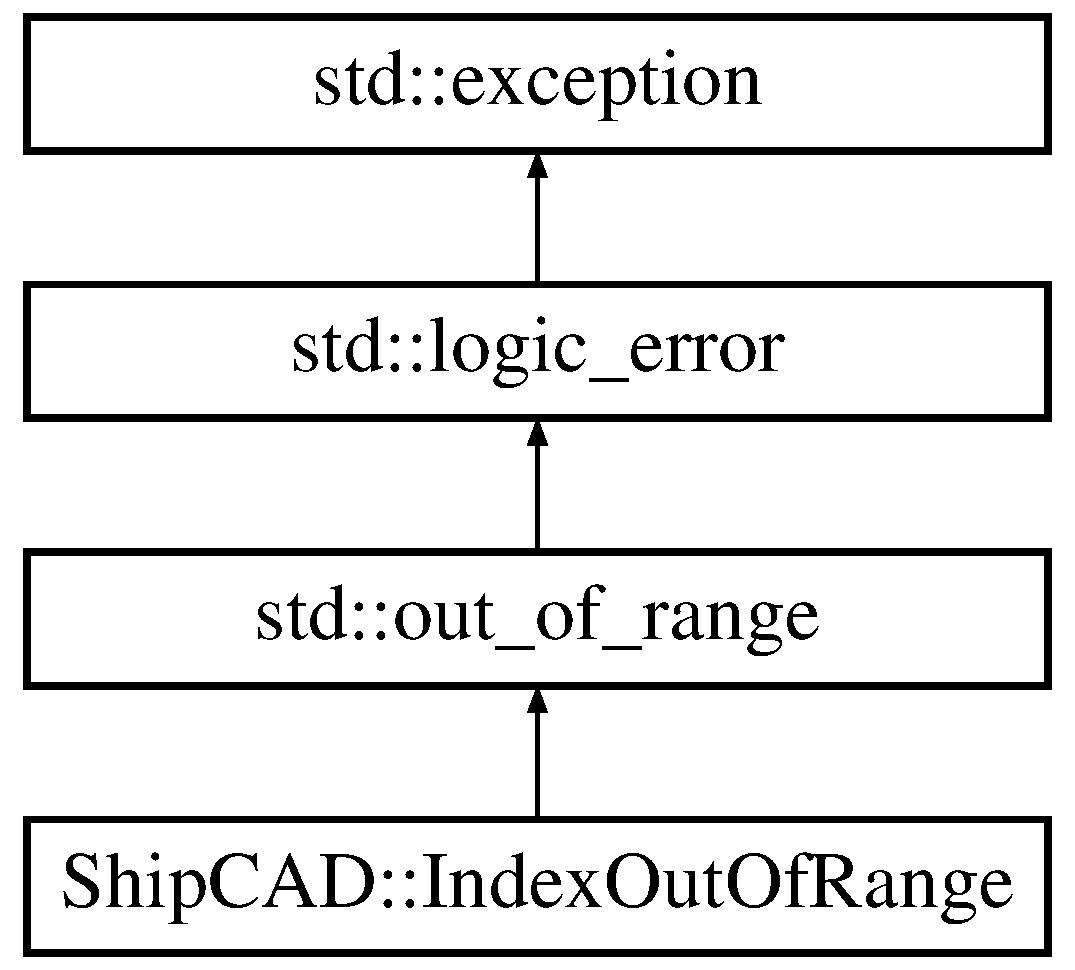
\includegraphics[height=4.000000cm]{classShipCAD_1_1IndexOutOfRange}
\end{center}
\end{figure}
\subsection*{Public Member Functions}
\begin{DoxyCompactItemize}
\item 
\hyperlink{classShipCAD_1_1IndexOutOfRange_a29a41ae3a4a0b8c2e2d9b407a6446496}{Index\-Out\-Of\-Range} (const std\-::string \&what\-\_\-arg)
\end{DoxyCompactItemize}


\subsection{Detailed Description}


Definition at line 50 of file exception.\-h.



\subsection{Constructor \& Destructor Documentation}
\hypertarget{classShipCAD_1_1IndexOutOfRange_a29a41ae3a4a0b8c2e2d9b407a6446496}{\index{Ship\-C\-A\-D\-::\-Index\-Out\-Of\-Range@{Ship\-C\-A\-D\-::\-Index\-Out\-Of\-Range}!Index\-Out\-Of\-Range@{Index\-Out\-Of\-Range}}
\index{Index\-Out\-Of\-Range@{Index\-Out\-Of\-Range}!ShipCAD::IndexOutOfRange@{Ship\-C\-A\-D\-::\-Index\-Out\-Of\-Range}}
\subsubsection[{Index\-Out\-Of\-Range}]{\setlength{\rightskip}{0pt plus 5cm}Ship\-C\-A\-D\-::\-Index\-Out\-Of\-Range\-::\-Index\-Out\-Of\-Range (
\begin{DoxyParamCaption}
\item[{const std\-::string \&}]{what\-\_\-arg}
\end{DoxyParamCaption}
)\hspace{0.3cm}{\ttfamily [inline]}}}\label{classShipCAD_1_1IndexOutOfRange_a29a41ae3a4a0b8c2e2d9b407a6446496}


Definition at line 53 of file exception.\-h.



The documentation for this class was generated from the following file\-:\begin{DoxyCompactItemize}
\item 
Ship\-C\-A\-Dlib/\hyperlink{exception_8h}{exception.\-h}\end{DoxyCompactItemize}

\hypertarget{classShipCAD_1_1Intersection}{\section{Ship\-C\-A\-D\-:\-:Intersection Class Reference}
\label{classShipCAD_1_1Intersection}\index{Ship\-C\-A\-D\-::\-Intersection@{Ship\-C\-A\-D\-::\-Intersection}}
}


List of curves intersecting hull.  




{\ttfamily \#include $<$intersection.\-h$>$}

Inheritance diagram for Ship\-C\-A\-D\-:\-:Intersection\-:\begin{figure}[H]
\begin{center}
\leavevmode
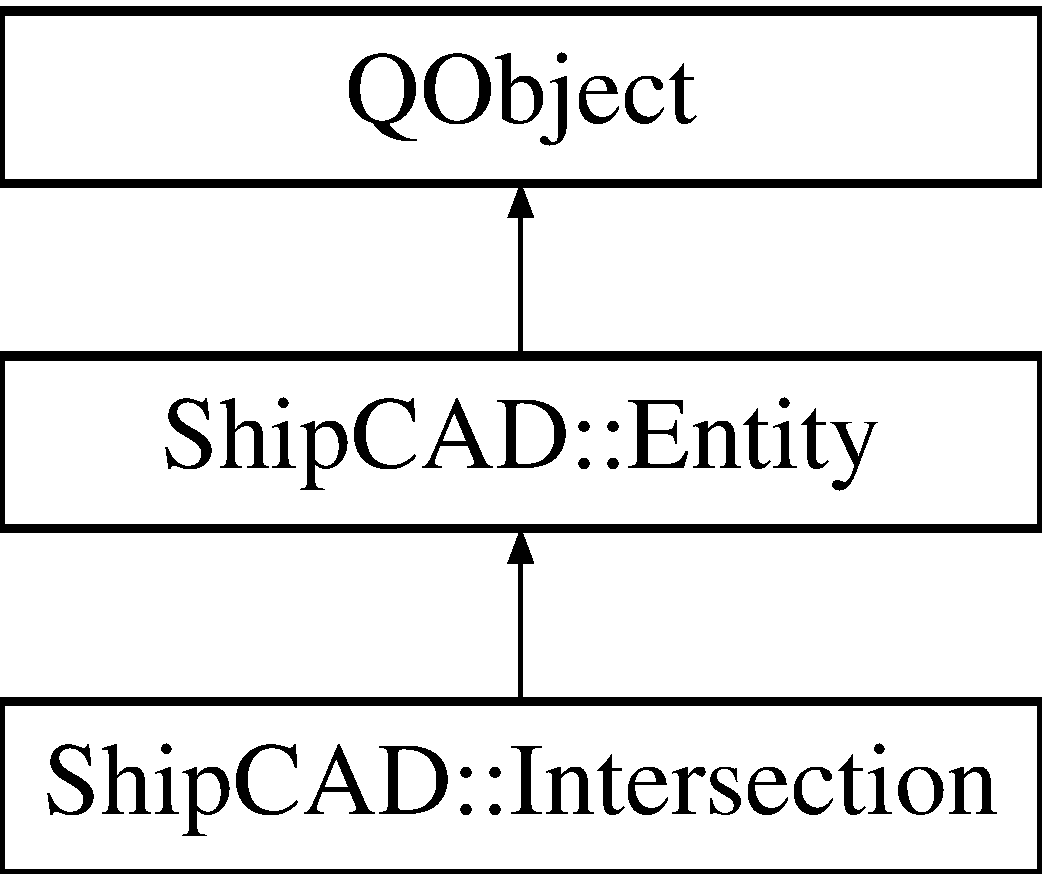
\includegraphics[height=3.000000cm]{classShipCAD_1_1Intersection}
\end{center}
\end{figure}
\subsection*{Public Member Functions}
\begin{DoxyCompactItemize}
\item 
\hyperlink{classShipCAD_1_1Intersection_acde7d35483e1e4ee56ecf75eb7a70f66}{Intersection} (\hyperlink{classShipCAD_1_1ShipCADModel}{Ship\-C\-A\-D\-Model} $\ast$owner)
\item 
\hyperlink{classShipCAD_1_1Intersection_a3a4f17fe81289d26d2ec329dd9db5c69}{Intersection} (\hyperlink{classShipCAD_1_1ShipCADModel}{Ship\-C\-A\-D\-Model} $\ast$owner, \hyperlink{namespaceShipCAD_aa56834b730aafdf2786ddc9a60a046fd}{intersection\-\_\-type\-\_\-t} ty, const \hyperlink{classShipCAD_1_1Plane}{Plane} \&pln, bool use\-\_\-hydrostatics\-\_\-only)
\item 
virtual \hyperlink{classShipCAD_1_1Intersection_a064951a970ed8dd11081b2903ab62122}{$\sim$\-Intersection} ()
\item 
virtual void \hyperlink{classShipCAD_1_1Intersection_a2163245dc7153d1590811ab2902d6ee4}{clear} ()
\item 
virtual void \hyperlink{classShipCAD_1_1Intersection_af751d515708531ca098321840a92c47b}{extents} (Q\-Vector3\-D \&min, Q\-Vector3\-D \&max)
\item 
virtual void \hyperlink{classShipCAD_1_1Intersection_a9e346019a52aa0540628b75994ea94a5}{draw} (\hyperlink{classShipCAD_1_1Viewport}{Viewport} \&vp, \hyperlink{classShipCAD_1_1LineShader}{Line\-Shader} $\ast$lineshader)
\item 
virtual void \hyperlink{classShipCAD_1_1Intersection_aed30bdca43037f72b85c4d53e234fd6c}{rebuild} ()
\item 
virtual void \hyperlink{classShipCAD_1_1Intersection_a2b496f9ab21c5fc4a7b97a665b24f2b1}{set\-Build} (bool val)
\item 
Q\-Color \hyperlink{classShipCAD_1_1Intersection_acae07360e9ccef12a498332ac6dbedd9}{get\-Color} ()
\item 
\hyperlink{classShipCAD_1_1Plane}{Plane} \hyperlink{classShipCAD_1_1Intersection_ac0b838a811f8df5c2fa0b0ea44ba4bb7}{get\-Plane} ()
\item 
void \hyperlink{classShipCAD_1_1Intersection_a582c3dcbe3016c554b6bba094e2854ce}{set\-Plane} (const \hyperlink{classShipCAD_1_1Plane}{Plane} \&pln)
\item 
Q\-String \hyperlink{classShipCAD_1_1Intersection_ab0434113cfd34c8a3ab11f75976dbf5b}{get\-Description} ()
\item 
\hyperlink{namespaceShipCAD_aa56834b730aafdf2786ddc9a60a046fd}{intersection\-\_\-type\-\_\-t} \hyperlink{classShipCAD_1_1Intersection_a1b93db56e5877226b30871754bba9838}{get\-Intersection\-Type} ()
\item 
void \hyperlink{classShipCAD_1_1Intersection_adc12c68675b19f5ae92d4c6ec8db0f62}{set\-Intersection\-Type} (\hyperlink{namespaceShipCAD_aa56834b730aafdf2786ddc9a60a046fd}{intersection\-\_\-type\-\_\-t} set)
\item 
bool \hyperlink{classShipCAD_1_1Intersection_a5ac5f3018d8b95b57ab40ccafe782bf4}{use\-Hydrostatics\-Surfaces\-Only} ()
\item 
void \hyperlink{classShipCAD_1_1Intersection_a8b587bbe80ef146d25e8a1568a84afb0}{set\-Use\-Hydrostatics\-Surfaces\-Only} (bool set)
\item 
\hyperlink{namespaceShipCAD_a053b941b2c87049bb9380428d4d5a056}{Spline\-Vector} \& \hyperlink{classShipCAD_1_1Intersection_a0092acbb149bb6a5c2e1f9a4b300c2da}{get\-Splines} ()
\item 
void \hyperlink{classShipCAD_1_1Intersection_ade472c721a5cb093c0b464c770c88634}{calculate\-Area} (const \hyperlink{classShipCAD_1_1Plane}{Plane} \&plane, float $\ast$area, Q\-Vector3\-D $\ast$cog, Q\-Vector2\-D $\ast$moment\-\_\-of\-\_\-inertia)
\item 
void \hyperlink{classShipCAD_1_1Intersection_a0af2af543403b3c69d1d3c786a1c6575}{create\-Starboard\-Part} ()
\item 
void \hyperlink{classShipCAD_1_1Intersection_ada420a69dc8141794aa617f966cbe2b2}{delete\-Item} (\hyperlink{classShipCAD_1_1Spline}{Spline} $\ast$item)
\item 
void \hyperlink{classShipCAD_1_1Intersection_a3e87aa28a1e1d721fe657a73d5466f3b}{load\-Binary} (\hyperlink{classShipCAD_1_1FileBuffer}{File\-Buffer} \&source)
\item 
void \hyperlink{classShipCAD_1_1Intersection_a41ce3a17845a7808d052713ae57dbe63}{save\-Binary} (\hyperlink{classShipCAD_1_1FileBuffer}{File\-Buffer} \&dest)
\item 
void \hyperlink{classShipCAD_1_1Intersection_a00a6d7ad7e82e43bd0287fa88dd87cf3}{save\-To\-D\-X\-F} (Q\-String\-List \&strings)
\end{DoxyCompactItemize}
\subsection*{Additional Inherited Members}


\subsection{Detailed Description}
List of curves intersecting hull. 

A list of curves from the intersection of the ships hull (represented by a subdivision surface) and a plane This plane can be a orthogonal plane (eg stations, waterlines, buttocks) or a freely oriented 3\-D plane 

Definition at line 58 of file intersection.\-h.



\subsection{Constructor \& Destructor Documentation}
\hypertarget{classShipCAD_1_1Intersection_acde7d35483e1e4ee56ecf75eb7a70f66}{\index{Ship\-C\-A\-D\-::\-Intersection@{Ship\-C\-A\-D\-::\-Intersection}!Intersection@{Intersection}}
\index{Intersection@{Intersection}!ShipCAD::Intersection@{Ship\-C\-A\-D\-::\-Intersection}}
\subsubsection[{Intersection}]{\setlength{\rightskip}{0pt plus 5cm}Intersection\-::\-Intersection (
\begin{DoxyParamCaption}
\item[{{\bf Ship\-C\-A\-D\-Model} $\ast$}]{owner}
\end{DoxyParamCaption}
)\hspace{0.3cm}{\ttfamily [explicit]}}}\label{classShipCAD_1_1Intersection_acde7d35483e1e4ee56ecf75eb7a70f66}


Definition at line 49 of file intersection.\-cpp.

\hypertarget{classShipCAD_1_1Intersection_a3a4f17fe81289d26d2ec329dd9db5c69}{\index{Ship\-C\-A\-D\-::\-Intersection@{Ship\-C\-A\-D\-::\-Intersection}!Intersection@{Intersection}}
\index{Intersection@{Intersection}!ShipCAD::Intersection@{Ship\-C\-A\-D\-::\-Intersection}}
\subsubsection[{Intersection}]{\setlength{\rightskip}{0pt plus 5cm}Intersection\-::\-Intersection (
\begin{DoxyParamCaption}
\item[{{\bf Ship\-C\-A\-D\-Model} $\ast$}]{owner, }
\item[{{\bf intersection\-\_\-type\-\_\-t}}]{ty, }
\item[{const {\bf Plane} \&}]{pln, }
\item[{bool}]{use\-\_\-hydrostatics\-\_\-only}
\end{DoxyParamCaption}
)\hspace{0.3cm}{\ttfamily [explicit]}}}\label{classShipCAD_1_1Intersection_a3a4f17fe81289d26d2ec329dd9db5c69}


Definition at line 56 of file intersection.\-cpp.

\hypertarget{classShipCAD_1_1Intersection_a064951a970ed8dd11081b2903ab62122}{\index{Ship\-C\-A\-D\-::\-Intersection@{Ship\-C\-A\-D\-::\-Intersection}!$\sim$\-Intersection@{$\sim$\-Intersection}}
\index{$\sim$\-Intersection@{$\sim$\-Intersection}!ShipCAD::Intersection@{Ship\-C\-A\-D\-::\-Intersection}}
\subsubsection[{$\sim$\-Intersection}]{\setlength{\rightskip}{0pt plus 5cm}Intersection\-::$\sim$\-Intersection (
\begin{DoxyParamCaption}
{}
\end{DoxyParamCaption}
)\hspace{0.3cm}{\ttfamily [virtual]}}}\label{classShipCAD_1_1Intersection_a064951a970ed8dd11081b2903ab62122}


Definition at line 63 of file intersection.\-cpp.



\subsection{Member Function Documentation}
\hypertarget{classShipCAD_1_1Intersection_ade472c721a5cb093c0b464c770c88634}{\index{Ship\-C\-A\-D\-::\-Intersection@{Ship\-C\-A\-D\-::\-Intersection}!calculate\-Area@{calculate\-Area}}
\index{calculate\-Area@{calculate\-Area}!ShipCAD::Intersection@{Ship\-C\-A\-D\-::\-Intersection}}
\subsubsection[{calculate\-Area}]{\setlength{\rightskip}{0pt plus 5cm}void Intersection\-::calculate\-Area (
\begin{DoxyParamCaption}
\item[{const {\bf Plane} \&}]{plane, }
\item[{float $\ast$}]{area, }
\item[{Q\-Vector3\-D $\ast$}]{cog, }
\item[{Q\-Vector2\-D $\ast$}]{moment\-\_\-of\-\_\-inertia}
\end{DoxyParamCaption}
)}}\label{classShipCAD_1_1Intersection_ade472c721a5cb093c0b464c770c88634}


Definition at line 259 of file intersection.\-cpp.

\hypertarget{classShipCAD_1_1Intersection_a2163245dc7153d1590811ab2902d6ee4}{\index{Ship\-C\-A\-D\-::\-Intersection@{Ship\-C\-A\-D\-::\-Intersection}!clear@{clear}}
\index{clear@{clear}!ShipCAD::Intersection@{Ship\-C\-A\-D\-::\-Intersection}}
\subsubsection[{clear}]{\setlength{\rightskip}{0pt plus 5cm}void Intersection\-::clear (
\begin{DoxyParamCaption}
{}
\end{DoxyParamCaption}
)\hspace{0.3cm}{\ttfamily [virtual]}}}\label{classShipCAD_1_1Intersection_a2163245dc7153d1590811ab2902d6ee4}


Reimplemented from \hyperlink{classShipCAD_1_1Entity_a998d0e5d360371046fd5835ba1e0877a}{Ship\-C\-A\-D\-::\-Entity}.



Definition at line 68 of file intersection.\-cpp.

\hypertarget{classShipCAD_1_1Intersection_a0af2af543403b3c69d1d3c786a1c6575}{\index{Ship\-C\-A\-D\-::\-Intersection@{Ship\-C\-A\-D\-::\-Intersection}!create\-Starboard\-Part@{create\-Starboard\-Part}}
\index{create\-Starboard\-Part@{create\-Starboard\-Part}!ShipCAD::Intersection@{Ship\-C\-A\-D\-::\-Intersection}}
\subsubsection[{create\-Starboard\-Part}]{\setlength{\rightskip}{0pt plus 5cm}void Intersection\-::create\-Starboard\-Part (
\begin{DoxyParamCaption}
{}
\end{DoxyParamCaption}
)}}\label{classShipCAD_1_1Intersection_a0af2af543403b3c69d1d3c786a1c6575}


Definition at line 295 of file intersection.\-cpp.

\hypertarget{classShipCAD_1_1Intersection_ada420a69dc8141794aa617f966cbe2b2}{\index{Ship\-C\-A\-D\-::\-Intersection@{Ship\-C\-A\-D\-::\-Intersection}!delete\-Item@{delete\-Item}}
\index{delete\-Item@{delete\-Item}!ShipCAD::Intersection@{Ship\-C\-A\-D\-::\-Intersection}}
\subsubsection[{delete\-Item}]{\setlength{\rightskip}{0pt plus 5cm}void Intersection\-::delete\-Item (
\begin{DoxyParamCaption}
\item[{{\bf Spline} $\ast$}]{item}
\end{DoxyParamCaption}
)}}\label{classShipCAD_1_1Intersection_ada420a69dc8141794aa617f966cbe2b2}


Definition at line 347 of file intersection.\-cpp.

\hypertarget{classShipCAD_1_1Intersection_a9e346019a52aa0540628b75994ea94a5}{\index{Ship\-C\-A\-D\-::\-Intersection@{Ship\-C\-A\-D\-::\-Intersection}!draw@{draw}}
\index{draw@{draw}!ShipCAD::Intersection@{Ship\-C\-A\-D\-::\-Intersection}}
\subsubsection[{draw}]{\setlength{\rightskip}{0pt plus 5cm}void Intersection\-::draw (
\begin{DoxyParamCaption}
\item[{{\bf Viewport} \&}]{vp, }
\item[{{\bf Line\-Shader} $\ast$}]{lineshader}
\end{DoxyParamCaption}
)\hspace{0.3cm}{\ttfamily [virtual]}}}\label{classShipCAD_1_1Intersection_a9e346019a52aa0540628b75994ea94a5}


Implements \hyperlink{classShipCAD_1_1Entity_aa62e306d991140dcd564360f8f6e7539}{Ship\-C\-A\-D\-::\-Entity}.



Definition at line 123 of file intersection.\-cpp.

\hypertarget{classShipCAD_1_1Intersection_af751d515708531ca098321840a92c47b}{\index{Ship\-C\-A\-D\-::\-Intersection@{Ship\-C\-A\-D\-::\-Intersection}!extents@{extents}}
\index{extents@{extents}!ShipCAD::Intersection@{Ship\-C\-A\-D\-::\-Intersection}}
\subsubsection[{extents}]{\setlength{\rightskip}{0pt plus 5cm}void Intersection\-::extents (
\begin{DoxyParamCaption}
\item[{Q\-Vector3\-D \&}]{min, }
\item[{Q\-Vector3\-D \&}]{max}
\end{DoxyParamCaption}
)\hspace{0.3cm}{\ttfamily [virtual]}}}\label{classShipCAD_1_1Intersection_af751d515708531ca098321840a92c47b}


Reimplemented from \hyperlink{classShipCAD_1_1Entity_a08e8e53770c85002afa45f46e7bf10f8}{Ship\-C\-A\-D\-::\-Entity}.



Definition at line 110 of file intersection.\-cpp.

\hypertarget{classShipCAD_1_1Intersection_acae07360e9ccef12a498332ac6dbedd9}{\index{Ship\-C\-A\-D\-::\-Intersection@{Ship\-C\-A\-D\-::\-Intersection}!get\-Color@{get\-Color}}
\index{get\-Color@{get\-Color}!ShipCAD::Intersection@{Ship\-C\-A\-D\-::\-Intersection}}
\subsubsection[{get\-Color}]{\setlength{\rightskip}{0pt plus 5cm}Q\-Color Intersection\-::get\-Color (
\begin{DoxyParamCaption}
{}
\end{DoxyParamCaption}
)}}\label{classShipCAD_1_1Intersection_acae07360e9ccef12a498332ac6dbedd9}


Definition at line 84 of file intersection.\-cpp.

\hypertarget{classShipCAD_1_1Intersection_ab0434113cfd34c8a3ab11f75976dbf5b}{\index{Ship\-C\-A\-D\-::\-Intersection@{Ship\-C\-A\-D\-::\-Intersection}!get\-Description@{get\-Description}}
\index{get\-Description@{get\-Description}!ShipCAD::Intersection@{Ship\-C\-A\-D\-::\-Intersection}}
\subsubsection[{get\-Description}]{\setlength{\rightskip}{0pt plus 5cm}Q\-String Intersection\-::get\-Description (
\begin{DoxyParamCaption}
{}
\end{DoxyParamCaption}
)}}\label{classShipCAD_1_1Intersection_ab0434113cfd34c8a3ab11f75976dbf5b}


Definition at line 118 of file intersection.\-cpp.

\hypertarget{classShipCAD_1_1Intersection_a1b93db56e5877226b30871754bba9838}{\index{Ship\-C\-A\-D\-::\-Intersection@{Ship\-C\-A\-D\-::\-Intersection}!get\-Intersection\-Type@{get\-Intersection\-Type}}
\index{get\-Intersection\-Type@{get\-Intersection\-Type}!ShipCAD::Intersection@{Ship\-C\-A\-D\-::\-Intersection}}
\subsubsection[{get\-Intersection\-Type}]{\setlength{\rightskip}{0pt plus 5cm}{\bf intersection\-\_\-type\-\_\-t} Ship\-C\-A\-D\-::\-Intersection\-::get\-Intersection\-Type (
\begin{DoxyParamCaption}
{}
\end{DoxyParamCaption}
)}}\label{classShipCAD_1_1Intersection_a1b93db56e5877226b30871754bba9838}
\hypertarget{classShipCAD_1_1Intersection_ac0b838a811f8df5c2fa0b0ea44ba4bb7}{\index{Ship\-C\-A\-D\-::\-Intersection@{Ship\-C\-A\-D\-::\-Intersection}!get\-Plane@{get\-Plane}}
\index{get\-Plane@{get\-Plane}!ShipCAD::Intersection@{Ship\-C\-A\-D\-::\-Intersection}}
\subsubsection[{get\-Plane}]{\setlength{\rightskip}{0pt plus 5cm}{\bf Plane} Ship\-C\-A\-D\-::\-Intersection\-::get\-Plane (
\begin{DoxyParamCaption}
{}
\end{DoxyParamCaption}
)\hspace{0.3cm}{\ttfamily [inline]}}}\label{classShipCAD_1_1Intersection_ac0b838a811f8df5c2fa0b0ea44ba4bb7}


Definition at line 75 of file intersection.\-h.

\hypertarget{classShipCAD_1_1Intersection_a0092acbb149bb6a5c2e1f9a4b300c2da}{\index{Ship\-C\-A\-D\-::\-Intersection@{Ship\-C\-A\-D\-::\-Intersection}!get\-Splines@{get\-Splines}}
\index{get\-Splines@{get\-Splines}!ShipCAD::Intersection@{Ship\-C\-A\-D\-::\-Intersection}}
\subsubsection[{get\-Splines}]{\setlength{\rightskip}{0pt plus 5cm}{\bf Spline\-Vector}\& Ship\-C\-A\-D\-::\-Intersection\-::get\-Splines (
\begin{DoxyParamCaption}
{}
\end{DoxyParamCaption}
)}}\label{classShipCAD_1_1Intersection_a0092acbb149bb6a5c2e1f9a4b300c2da}
\hypertarget{classShipCAD_1_1Intersection_a3e87aa28a1e1d721fe657a73d5466f3b}{\index{Ship\-C\-A\-D\-::\-Intersection@{Ship\-C\-A\-D\-::\-Intersection}!load\-Binary@{load\-Binary}}
\index{load\-Binary@{load\-Binary}!ShipCAD::Intersection@{Ship\-C\-A\-D\-::\-Intersection}}
\subsubsection[{load\-Binary}]{\setlength{\rightskip}{0pt plus 5cm}void Intersection\-::load\-Binary (
\begin{DoxyParamCaption}
\item[{{\bf File\-Buffer} \&}]{source}
\end{DoxyParamCaption}
)}}\label{classShipCAD_1_1Intersection_a3e87aa28a1e1d721fe657a73d5466f3b}


Definition at line 352 of file intersection.\-cpp.

\hypertarget{classShipCAD_1_1Intersection_aed30bdca43037f72b85c4d53e234fd6c}{\index{Ship\-C\-A\-D\-::\-Intersection@{Ship\-C\-A\-D\-::\-Intersection}!rebuild@{rebuild}}
\index{rebuild@{rebuild}!ShipCAD::Intersection@{Ship\-C\-A\-D\-::\-Intersection}}
\subsubsection[{rebuild}]{\setlength{\rightskip}{0pt plus 5cm}void Intersection\-::rebuild (
\begin{DoxyParamCaption}
{}
\end{DoxyParamCaption}
)\hspace{0.3cm}{\ttfamily [virtual]}}}\label{classShipCAD_1_1Intersection_aed30bdca43037f72b85c4d53e234fd6c}


Implements \hyperlink{classShipCAD_1_1Entity_a2571654319df6ad6841a437be7a75395}{Ship\-C\-A\-D\-::\-Entity}.



Definition at line 133 of file intersection.\-cpp.

\hypertarget{classShipCAD_1_1Intersection_a41ce3a17845a7808d052713ae57dbe63}{\index{Ship\-C\-A\-D\-::\-Intersection@{Ship\-C\-A\-D\-::\-Intersection}!save\-Binary@{save\-Binary}}
\index{save\-Binary@{save\-Binary}!ShipCAD::Intersection@{Ship\-C\-A\-D\-::\-Intersection}}
\subsubsection[{save\-Binary}]{\setlength{\rightskip}{0pt plus 5cm}void Intersection\-::save\-Binary (
\begin{DoxyParamCaption}
\item[{{\bf File\-Buffer} \&}]{dest}
\end{DoxyParamCaption}
)}}\label{classShipCAD_1_1Intersection_a41ce3a17845a7808d052713ae57dbe63}


Definition at line 407 of file intersection.\-cpp.

\hypertarget{classShipCAD_1_1Intersection_a00a6d7ad7e82e43bd0287fa88dd87cf3}{\index{Ship\-C\-A\-D\-::\-Intersection@{Ship\-C\-A\-D\-::\-Intersection}!save\-To\-D\-X\-F@{save\-To\-D\-X\-F}}
\index{save\-To\-D\-X\-F@{save\-To\-D\-X\-F}!ShipCAD::Intersection@{Ship\-C\-A\-D\-::\-Intersection}}
\subsubsection[{save\-To\-D\-X\-F}]{\setlength{\rightskip}{0pt plus 5cm}void Intersection\-::save\-To\-D\-X\-F (
\begin{DoxyParamCaption}
\item[{Q\-String\-List \&}]{strings}
\end{DoxyParamCaption}
)}}\label{classShipCAD_1_1Intersection_a00a6d7ad7e82e43bd0287fa88dd87cf3}


Definition at line 450 of file intersection.\-cpp.

\hypertarget{classShipCAD_1_1Intersection_a2b496f9ab21c5fc4a7b97a665b24f2b1}{\index{Ship\-C\-A\-D\-::\-Intersection@{Ship\-C\-A\-D\-::\-Intersection}!set\-Build@{set\-Build}}
\index{set\-Build@{set\-Build}!ShipCAD::Intersection@{Ship\-C\-A\-D\-::\-Intersection}}
\subsubsection[{set\-Build}]{\setlength{\rightskip}{0pt plus 5cm}void Intersection\-::set\-Build (
\begin{DoxyParamCaption}
\item[{bool}]{val}
\end{DoxyParamCaption}
)\hspace{0.3cm}{\ttfamily [virtual]}}}\label{classShipCAD_1_1Intersection_a2b496f9ab21c5fc4a7b97a665b24f2b1}


Reimplemented from \hyperlink{classShipCAD_1_1Entity_a1889198398f42bb7f77a2334031c3f33}{Ship\-C\-A\-D\-::\-Entity}.



Definition at line 77 of file intersection.\-cpp.

\hypertarget{classShipCAD_1_1Intersection_adc12c68675b19f5ae92d4c6ec8db0f62}{\index{Ship\-C\-A\-D\-::\-Intersection@{Ship\-C\-A\-D\-::\-Intersection}!set\-Intersection\-Type@{set\-Intersection\-Type}}
\index{set\-Intersection\-Type@{set\-Intersection\-Type}!ShipCAD::Intersection@{Ship\-C\-A\-D\-::\-Intersection}}
\subsubsection[{set\-Intersection\-Type}]{\setlength{\rightskip}{0pt plus 5cm}void Ship\-C\-A\-D\-::\-Intersection\-::set\-Intersection\-Type (
\begin{DoxyParamCaption}
\item[{{\bf intersection\-\_\-type\-\_\-t}}]{set}
\end{DoxyParamCaption}
)}}\label{classShipCAD_1_1Intersection_adc12c68675b19f5ae92d4c6ec8db0f62}
\hypertarget{classShipCAD_1_1Intersection_a582c3dcbe3016c554b6bba094e2854ce}{\index{Ship\-C\-A\-D\-::\-Intersection@{Ship\-C\-A\-D\-::\-Intersection}!set\-Plane@{set\-Plane}}
\index{set\-Plane@{set\-Plane}!ShipCAD::Intersection@{Ship\-C\-A\-D\-::\-Intersection}}
\subsubsection[{set\-Plane}]{\setlength{\rightskip}{0pt plus 5cm}void Ship\-C\-A\-D\-::\-Intersection\-::set\-Plane (
\begin{DoxyParamCaption}
\item[{const {\bf Plane} \&}]{pln}
\end{DoxyParamCaption}
)}}\label{classShipCAD_1_1Intersection_a582c3dcbe3016c554b6bba094e2854ce}
\hypertarget{classShipCAD_1_1Intersection_a8b587bbe80ef146d25e8a1568a84afb0}{\index{Ship\-C\-A\-D\-::\-Intersection@{Ship\-C\-A\-D\-::\-Intersection}!set\-Use\-Hydrostatics\-Surfaces\-Only@{set\-Use\-Hydrostatics\-Surfaces\-Only}}
\index{set\-Use\-Hydrostatics\-Surfaces\-Only@{set\-Use\-Hydrostatics\-Surfaces\-Only}!ShipCAD::Intersection@{Ship\-C\-A\-D\-::\-Intersection}}
\subsubsection[{set\-Use\-Hydrostatics\-Surfaces\-Only}]{\setlength{\rightskip}{0pt plus 5cm}void Ship\-C\-A\-D\-::\-Intersection\-::set\-Use\-Hydrostatics\-Surfaces\-Only (
\begin{DoxyParamCaption}
\item[{bool}]{set}
\end{DoxyParamCaption}
)}}\label{classShipCAD_1_1Intersection_a8b587bbe80ef146d25e8a1568a84afb0}
\hypertarget{classShipCAD_1_1Intersection_a5ac5f3018d8b95b57ab40ccafe782bf4}{\index{Ship\-C\-A\-D\-::\-Intersection@{Ship\-C\-A\-D\-::\-Intersection}!use\-Hydrostatics\-Surfaces\-Only@{use\-Hydrostatics\-Surfaces\-Only}}
\index{use\-Hydrostatics\-Surfaces\-Only@{use\-Hydrostatics\-Surfaces\-Only}!ShipCAD::Intersection@{Ship\-C\-A\-D\-::\-Intersection}}
\subsubsection[{use\-Hydrostatics\-Surfaces\-Only}]{\setlength{\rightskip}{0pt plus 5cm}bool Ship\-C\-A\-D\-::\-Intersection\-::use\-Hydrostatics\-Surfaces\-Only (
\begin{DoxyParamCaption}
{}
\end{DoxyParamCaption}
)}}\label{classShipCAD_1_1Intersection_a5ac5f3018d8b95b57ab40ccafe782bf4}


The documentation for this class was generated from the following files\-:\begin{DoxyCompactItemize}
\item 
Ship\-C\-A\-Dlib/\hyperlink{intersection_8h}{intersection.\-h}\item 
Ship\-C\-A\-Dlib/\hyperlink{intersection_8cpp}{intersection.\-cpp}\end{DoxyCompactItemize}

\hypertarget{classShipCAD_1_1IntersectionData}{\section{Ship\-C\-A\-D\-:\-:Intersection\-Data Class Reference}
\label{classShipCAD_1_1IntersectionData}\index{Ship\-C\-A\-D\-::\-Intersection\-Data@{Ship\-C\-A\-D\-::\-Intersection\-Data}}
}


Structure to record geometry intersections.  




{\ttfamily \#include $<$entity.\-h$>$}

\subsection*{Public Member Functions}
\begin{DoxyCompactItemize}
\item 
\hyperlink{classShipCAD_1_1IntersectionData_acc582d8820d6e60117e0bf5fe686ab76}{Intersection\-Data} ()
\item 
\hyperlink{classShipCAD_1_1IntersectionData_a80ee22151368715711e3713eae61d401}{$\sim$\-Intersection\-Data} ()
\end{DoxyCompactItemize}
\subsection*{Public Attributes}
\begin{DoxyCompactItemize}
\item 
size\-\_\-t \hyperlink{classShipCAD_1_1IntersectionData_a5b42e3b8b81d18963f9a07609b402628}{number\-\_\-of\-\_\-intersections}
\item 
std\-::vector$<$ Q\-Vector3\-D $>$ \hyperlink{classShipCAD_1_1IntersectionData_a926e126e42d95e01b39e2750a0e1fb95}{points}
\item 
std\-::vector$<$ float $>$ \hyperlink{classShipCAD_1_1IntersectionData_a06fcbb71243644bdea0e5b86da3b191c}{parameters}
\end{DoxyCompactItemize}


\subsection{Detailed Description}
Structure to record geometry intersections. 

Definition at line 49 of file entity.\-h.



\subsection{Constructor \& Destructor Documentation}
\hypertarget{classShipCAD_1_1IntersectionData_acc582d8820d6e60117e0bf5fe686ab76}{\index{Ship\-C\-A\-D\-::\-Intersection\-Data@{Ship\-C\-A\-D\-::\-Intersection\-Data}!Intersection\-Data@{Intersection\-Data}}
\index{Intersection\-Data@{Intersection\-Data}!ShipCAD::IntersectionData@{Ship\-C\-A\-D\-::\-Intersection\-Data}}
\subsubsection[{Intersection\-Data}]{\setlength{\rightskip}{0pt plus 5cm}Ship\-C\-A\-D\-::\-Intersection\-Data\-::\-Intersection\-Data (
\begin{DoxyParamCaption}
{}
\end{DoxyParamCaption}
)\hspace{0.3cm}{\ttfamily [inline]}, {\ttfamily [explicit]}}}\label{classShipCAD_1_1IntersectionData_acc582d8820d6e60117e0bf5fe686ab76}


Definition at line 53 of file entity.\-h.

\hypertarget{classShipCAD_1_1IntersectionData_a80ee22151368715711e3713eae61d401}{\index{Ship\-C\-A\-D\-::\-Intersection\-Data@{Ship\-C\-A\-D\-::\-Intersection\-Data}!$\sim$\-Intersection\-Data@{$\sim$\-Intersection\-Data}}
\index{$\sim$\-Intersection\-Data@{$\sim$\-Intersection\-Data}!ShipCAD::IntersectionData@{Ship\-C\-A\-D\-::\-Intersection\-Data}}
\subsubsection[{$\sim$\-Intersection\-Data}]{\setlength{\rightskip}{0pt plus 5cm}Ship\-C\-A\-D\-::\-Intersection\-Data\-::$\sim$\-Intersection\-Data (
\begin{DoxyParamCaption}
{}
\end{DoxyParamCaption}
)\hspace{0.3cm}{\ttfamily [inline]}}}\label{classShipCAD_1_1IntersectionData_a80ee22151368715711e3713eae61d401}


Definition at line 54 of file entity.\-h.



\subsection{Member Data Documentation}
\hypertarget{classShipCAD_1_1IntersectionData_a5b42e3b8b81d18963f9a07609b402628}{\index{Ship\-C\-A\-D\-::\-Intersection\-Data@{Ship\-C\-A\-D\-::\-Intersection\-Data}!number\-\_\-of\-\_\-intersections@{number\-\_\-of\-\_\-intersections}}
\index{number\-\_\-of\-\_\-intersections@{number\-\_\-of\-\_\-intersections}!ShipCAD::IntersectionData@{Ship\-C\-A\-D\-::\-Intersection\-Data}}
\subsubsection[{number\-\_\-of\-\_\-intersections}]{\setlength{\rightskip}{0pt plus 5cm}size\-\_\-t Ship\-C\-A\-D\-::\-Intersection\-Data\-::number\-\_\-of\-\_\-intersections}}\label{classShipCAD_1_1IntersectionData_a5b42e3b8b81d18963f9a07609b402628}


Definition at line 56 of file entity.\-h.

\hypertarget{classShipCAD_1_1IntersectionData_a06fcbb71243644bdea0e5b86da3b191c}{\index{Ship\-C\-A\-D\-::\-Intersection\-Data@{Ship\-C\-A\-D\-::\-Intersection\-Data}!parameters@{parameters}}
\index{parameters@{parameters}!ShipCAD::IntersectionData@{Ship\-C\-A\-D\-::\-Intersection\-Data}}
\subsubsection[{parameters}]{\setlength{\rightskip}{0pt plus 5cm}std\-::vector$<$float$>$ Ship\-C\-A\-D\-::\-Intersection\-Data\-::parameters}}\label{classShipCAD_1_1IntersectionData_a06fcbb71243644bdea0e5b86da3b191c}


Definition at line 58 of file entity.\-h.

\hypertarget{classShipCAD_1_1IntersectionData_a926e126e42d95e01b39e2750a0e1fb95}{\index{Ship\-C\-A\-D\-::\-Intersection\-Data@{Ship\-C\-A\-D\-::\-Intersection\-Data}!points@{points}}
\index{points@{points}!ShipCAD::IntersectionData@{Ship\-C\-A\-D\-::\-Intersection\-Data}}
\subsubsection[{points}]{\setlength{\rightskip}{0pt plus 5cm}std\-::vector$<$Q\-Vector3\-D$>$ Ship\-C\-A\-D\-::\-Intersection\-Data\-::points}}\label{classShipCAD_1_1IntersectionData_a926e126e42d95e01b39e2750a0e1fb95}


Definition at line 57 of file entity.\-h.



The documentation for this class was generated from the following file\-:\begin{DoxyCompactItemize}
\item 
Ship\-C\-A\-Dlib/\hyperlink{entity_8h}{entity.\-h}\end{DoxyCompactItemize}

\hypertarget{structShipCAD_1_1KAPERResistance}{\section{Ship\-C\-A\-D\-:\-:K\-A\-P\-E\-R\-Resistance Struct Reference}
\label{structShipCAD_1_1KAPERResistance}\index{Ship\-C\-A\-D\-::\-K\-A\-P\-E\-R\-Resistance@{Ship\-C\-A\-D\-::\-K\-A\-P\-E\-R\-Resistance}}
}


{\ttfamily \#include $<$resistance.\-h$>$}

\subsection*{Public Attributes}
\begin{DoxyCompactItemize}
\item 
float \hyperlink{structShipCAD_1_1KAPERResistance_a0be8d3ba3d4e485abe71c462575b478a}{draft}
\item 
float \hyperlink{structShipCAD_1_1KAPERResistance_a1c2aa0aa33bf7770cd531f1d1ea8b809}{lwl}
\item 
float \hyperlink{structShipCAD_1_1KAPERResistance_ab1cc995ebce998cfc19ef8b1501f328e}{bwl}
\item 
float \hyperlink{structShipCAD_1_1KAPERResistance_a07797d6eb31e9a5506f7fca4b92d3f3a}{cp}
\item 
float \hyperlink{structShipCAD_1_1KAPERResistance_a5227818b90eab4991e339bbdf2e382ca}{displacement}
\item 
float \hyperlink{structShipCAD_1_1KAPERResistance_a3b351285dc50665147ce987e0744b314}{lcb}
\item 
float \hyperlink{structShipCAD_1_1KAPERResistance_a912090d77ad755a5b1506372c24540bc}{wetted\-\_\-surface}
\item 
float \hyperlink{structShipCAD_1_1KAPERResistance_a803e780e97a79538c29af4a28c0afd51}{at\-\_\-ax}
\item 
float \hyperlink{structShipCAD_1_1KAPERResistance_a941bc6efce4bc30f542cae5c68218aee}{entrance\-\_\-angle}
\item 
bool \hyperlink{structShipCAD_1_1KAPERResistance_a61ce222b79ad3964b278f5239dd2618f}{extract}
\end{DoxyCompactItemize}


\subsection{Detailed Description}


Definition at line 59 of file resistance.\-h.



\subsection{Member Data Documentation}
\hypertarget{structShipCAD_1_1KAPERResistance_a803e780e97a79538c29af4a28c0afd51}{\index{Ship\-C\-A\-D\-::\-K\-A\-P\-E\-R\-Resistance@{Ship\-C\-A\-D\-::\-K\-A\-P\-E\-R\-Resistance}!at\-\_\-ax@{at\-\_\-ax}}
\index{at\-\_\-ax@{at\-\_\-ax}!ShipCAD::KAPERResistance@{Ship\-C\-A\-D\-::\-K\-A\-P\-E\-R\-Resistance}}
\subsubsection[{at\-\_\-ax}]{\setlength{\rightskip}{0pt plus 5cm}float Ship\-C\-A\-D\-::\-K\-A\-P\-E\-R\-Resistance\-::at\-\_\-ax}}\label{structShipCAD_1_1KAPERResistance_a803e780e97a79538c29af4a28c0afd51}


Definition at line 68 of file resistance.\-h.

\hypertarget{structShipCAD_1_1KAPERResistance_ab1cc995ebce998cfc19ef8b1501f328e}{\index{Ship\-C\-A\-D\-::\-K\-A\-P\-E\-R\-Resistance@{Ship\-C\-A\-D\-::\-K\-A\-P\-E\-R\-Resistance}!bwl@{bwl}}
\index{bwl@{bwl}!ShipCAD::KAPERResistance@{Ship\-C\-A\-D\-::\-K\-A\-P\-E\-R\-Resistance}}
\subsubsection[{bwl}]{\setlength{\rightskip}{0pt plus 5cm}float Ship\-C\-A\-D\-::\-K\-A\-P\-E\-R\-Resistance\-::bwl}}\label{structShipCAD_1_1KAPERResistance_ab1cc995ebce998cfc19ef8b1501f328e}


Definition at line 63 of file resistance.\-h.

\hypertarget{structShipCAD_1_1KAPERResistance_a07797d6eb31e9a5506f7fca4b92d3f3a}{\index{Ship\-C\-A\-D\-::\-K\-A\-P\-E\-R\-Resistance@{Ship\-C\-A\-D\-::\-K\-A\-P\-E\-R\-Resistance}!cp@{cp}}
\index{cp@{cp}!ShipCAD::KAPERResistance@{Ship\-C\-A\-D\-::\-K\-A\-P\-E\-R\-Resistance}}
\subsubsection[{cp}]{\setlength{\rightskip}{0pt plus 5cm}float Ship\-C\-A\-D\-::\-K\-A\-P\-E\-R\-Resistance\-::cp}}\label{structShipCAD_1_1KAPERResistance_a07797d6eb31e9a5506f7fca4b92d3f3a}


Definition at line 64 of file resistance.\-h.

\hypertarget{structShipCAD_1_1KAPERResistance_a5227818b90eab4991e339bbdf2e382ca}{\index{Ship\-C\-A\-D\-::\-K\-A\-P\-E\-R\-Resistance@{Ship\-C\-A\-D\-::\-K\-A\-P\-E\-R\-Resistance}!displacement@{displacement}}
\index{displacement@{displacement}!ShipCAD::KAPERResistance@{Ship\-C\-A\-D\-::\-K\-A\-P\-E\-R\-Resistance}}
\subsubsection[{displacement}]{\setlength{\rightskip}{0pt plus 5cm}float Ship\-C\-A\-D\-::\-K\-A\-P\-E\-R\-Resistance\-::displacement}}\label{structShipCAD_1_1KAPERResistance_a5227818b90eab4991e339bbdf2e382ca}


Definition at line 65 of file resistance.\-h.

\hypertarget{structShipCAD_1_1KAPERResistance_a0be8d3ba3d4e485abe71c462575b478a}{\index{Ship\-C\-A\-D\-::\-K\-A\-P\-E\-R\-Resistance@{Ship\-C\-A\-D\-::\-K\-A\-P\-E\-R\-Resistance}!draft@{draft}}
\index{draft@{draft}!ShipCAD::KAPERResistance@{Ship\-C\-A\-D\-::\-K\-A\-P\-E\-R\-Resistance}}
\subsubsection[{draft}]{\setlength{\rightskip}{0pt plus 5cm}float Ship\-C\-A\-D\-::\-K\-A\-P\-E\-R\-Resistance\-::draft}}\label{structShipCAD_1_1KAPERResistance_a0be8d3ba3d4e485abe71c462575b478a}


Definition at line 61 of file resistance.\-h.

\hypertarget{structShipCAD_1_1KAPERResistance_a941bc6efce4bc30f542cae5c68218aee}{\index{Ship\-C\-A\-D\-::\-K\-A\-P\-E\-R\-Resistance@{Ship\-C\-A\-D\-::\-K\-A\-P\-E\-R\-Resistance}!entrance\-\_\-angle@{entrance\-\_\-angle}}
\index{entrance\-\_\-angle@{entrance\-\_\-angle}!ShipCAD::KAPERResistance@{Ship\-C\-A\-D\-::\-K\-A\-P\-E\-R\-Resistance}}
\subsubsection[{entrance\-\_\-angle}]{\setlength{\rightskip}{0pt plus 5cm}float Ship\-C\-A\-D\-::\-K\-A\-P\-E\-R\-Resistance\-::entrance\-\_\-angle}}\label{structShipCAD_1_1KAPERResistance_a941bc6efce4bc30f542cae5c68218aee}


Definition at line 69 of file resistance.\-h.

\hypertarget{structShipCAD_1_1KAPERResistance_a61ce222b79ad3964b278f5239dd2618f}{\index{Ship\-C\-A\-D\-::\-K\-A\-P\-E\-R\-Resistance@{Ship\-C\-A\-D\-::\-K\-A\-P\-E\-R\-Resistance}!extract@{extract}}
\index{extract@{extract}!ShipCAD::KAPERResistance@{Ship\-C\-A\-D\-::\-K\-A\-P\-E\-R\-Resistance}}
\subsubsection[{extract}]{\setlength{\rightskip}{0pt plus 5cm}bool Ship\-C\-A\-D\-::\-K\-A\-P\-E\-R\-Resistance\-::extract}}\label{structShipCAD_1_1KAPERResistance_a61ce222b79ad3964b278f5239dd2618f}


Definition at line 70 of file resistance.\-h.

\hypertarget{structShipCAD_1_1KAPERResistance_a3b351285dc50665147ce987e0744b314}{\index{Ship\-C\-A\-D\-::\-K\-A\-P\-E\-R\-Resistance@{Ship\-C\-A\-D\-::\-K\-A\-P\-E\-R\-Resistance}!lcb@{lcb}}
\index{lcb@{lcb}!ShipCAD::KAPERResistance@{Ship\-C\-A\-D\-::\-K\-A\-P\-E\-R\-Resistance}}
\subsubsection[{lcb}]{\setlength{\rightskip}{0pt plus 5cm}float Ship\-C\-A\-D\-::\-K\-A\-P\-E\-R\-Resistance\-::lcb}}\label{structShipCAD_1_1KAPERResistance_a3b351285dc50665147ce987e0744b314}


Definition at line 66 of file resistance.\-h.

\hypertarget{structShipCAD_1_1KAPERResistance_a1c2aa0aa33bf7770cd531f1d1ea8b809}{\index{Ship\-C\-A\-D\-::\-K\-A\-P\-E\-R\-Resistance@{Ship\-C\-A\-D\-::\-K\-A\-P\-E\-R\-Resistance}!lwl@{lwl}}
\index{lwl@{lwl}!ShipCAD::KAPERResistance@{Ship\-C\-A\-D\-::\-K\-A\-P\-E\-R\-Resistance}}
\subsubsection[{lwl}]{\setlength{\rightskip}{0pt plus 5cm}float Ship\-C\-A\-D\-::\-K\-A\-P\-E\-R\-Resistance\-::lwl}}\label{structShipCAD_1_1KAPERResistance_a1c2aa0aa33bf7770cd531f1d1ea8b809}


Definition at line 62 of file resistance.\-h.

\hypertarget{structShipCAD_1_1KAPERResistance_a912090d77ad755a5b1506372c24540bc}{\index{Ship\-C\-A\-D\-::\-K\-A\-P\-E\-R\-Resistance@{Ship\-C\-A\-D\-::\-K\-A\-P\-E\-R\-Resistance}!wetted\-\_\-surface@{wetted\-\_\-surface}}
\index{wetted\-\_\-surface@{wetted\-\_\-surface}!ShipCAD::KAPERResistance@{Ship\-C\-A\-D\-::\-K\-A\-P\-E\-R\-Resistance}}
\subsubsection[{wetted\-\_\-surface}]{\setlength{\rightskip}{0pt plus 5cm}float Ship\-C\-A\-D\-::\-K\-A\-P\-E\-R\-Resistance\-::wetted\-\_\-surface}}\label{structShipCAD_1_1KAPERResistance_a912090d77ad755a5b1506372c24540bc}


Definition at line 67 of file resistance.\-h.



The documentation for this struct was generated from the following file\-:\begin{DoxyCompactItemize}
\item 
Ship\-C\-A\-Dlib/\hyperlink{resistance_8h}{resistance.\-h}\end{DoxyCompactItemize}

\hypertarget{structShipCAD_1_1LayerProperties}{\section{Ship\-C\-A\-D\-:\-:Layer\-Properties Struct Reference}
\label{structShipCAD_1_1LayerProperties}\index{Ship\-C\-A\-D\-::\-Layer\-Properties@{Ship\-C\-A\-D\-::\-Layer\-Properties}}
}


{\ttfamily \#include $<$subdivlayer.\-h$>$}

\subsection*{Public Member Functions}
\begin{DoxyCompactItemize}
\item 
\hyperlink{structShipCAD_1_1LayerProperties_ad48a1f9351ff4270868f56bd1211af09}{Layer\-Properties} ()
\end{DoxyCompactItemize}
\subsection*{Public Attributes}
\begin{DoxyCompactItemize}
\item 
float \hyperlink{structShipCAD_1_1LayerProperties_aff6dab68937efc1abd7bb5066373f514}{surface\-\_\-area}
\item 
float \hyperlink{structShipCAD_1_1LayerProperties_a4e9844dd95994725401ad93c5c3a00e9}{weight}
\item 
Q\-Vector3\-D \hyperlink{structShipCAD_1_1LayerProperties_a1b4bc8254c8cb90df594bc7905ce3e22}{surface\-\_\-center\-\_\-of\-\_\-gravity}
\end{DoxyCompactItemize}


\subsection{Detailed Description}


Definition at line 52 of file subdivlayer.\-h.



\subsection{Constructor \& Destructor Documentation}
\hypertarget{structShipCAD_1_1LayerProperties_ad48a1f9351ff4270868f56bd1211af09}{\index{Ship\-C\-A\-D\-::\-Layer\-Properties@{Ship\-C\-A\-D\-::\-Layer\-Properties}!Layer\-Properties@{Layer\-Properties}}
\index{Layer\-Properties@{Layer\-Properties}!ShipCAD::LayerProperties@{Ship\-C\-A\-D\-::\-Layer\-Properties}}
\subsubsection[{Layer\-Properties}]{\setlength{\rightskip}{0pt plus 5cm}Ship\-C\-A\-D\-::\-Layer\-Properties\-::\-Layer\-Properties (
\begin{DoxyParamCaption}
{}
\end{DoxyParamCaption}
)\hspace{0.3cm}{\ttfamily [inline]}}}\label{structShipCAD_1_1LayerProperties_ad48a1f9351ff4270868f56bd1211af09}


Definition at line 57 of file subdivlayer.\-h.



\subsection{Member Data Documentation}
\hypertarget{structShipCAD_1_1LayerProperties_aff6dab68937efc1abd7bb5066373f514}{\index{Ship\-C\-A\-D\-::\-Layer\-Properties@{Ship\-C\-A\-D\-::\-Layer\-Properties}!surface\-\_\-area@{surface\-\_\-area}}
\index{surface\-\_\-area@{surface\-\_\-area}!ShipCAD::LayerProperties@{Ship\-C\-A\-D\-::\-Layer\-Properties}}
\subsubsection[{surface\-\_\-area}]{\setlength{\rightskip}{0pt plus 5cm}float Ship\-C\-A\-D\-::\-Layer\-Properties\-::surface\-\_\-area}}\label{structShipCAD_1_1LayerProperties_aff6dab68937efc1abd7bb5066373f514}


Definition at line 54 of file subdivlayer.\-h.

\hypertarget{structShipCAD_1_1LayerProperties_a1b4bc8254c8cb90df594bc7905ce3e22}{\index{Ship\-C\-A\-D\-::\-Layer\-Properties@{Ship\-C\-A\-D\-::\-Layer\-Properties}!surface\-\_\-center\-\_\-of\-\_\-gravity@{surface\-\_\-center\-\_\-of\-\_\-gravity}}
\index{surface\-\_\-center\-\_\-of\-\_\-gravity@{surface\-\_\-center\-\_\-of\-\_\-gravity}!ShipCAD::LayerProperties@{Ship\-C\-A\-D\-::\-Layer\-Properties}}
\subsubsection[{surface\-\_\-center\-\_\-of\-\_\-gravity}]{\setlength{\rightskip}{0pt plus 5cm}Q\-Vector3\-D Ship\-C\-A\-D\-::\-Layer\-Properties\-::surface\-\_\-center\-\_\-of\-\_\-gravity}}\label{structShipCAD_1_1LayerProperties_a1b4bc8254c8cb90df594bc7905ce3e22}


Definition at line 56 of file subdivlayer.\-h.

\hypertarget{structShipCAD_1_1LayerProperties_a4e9844dd95994725401ad93c5c3a00e9}{\index{Ship\-C\-A\-D\-::\-Layer\-Properties@{Ship\-C\-A\-D\-::\-Layer\-Properties}!weight@{weight}}
\index{weight@{weight}!ShipCAD::LayerProperties@{Ship\-C\-A\-D\-::\-Layer\-Properties}}
\subsubsection[{weight}]{\setlength{\rightskip}{0pt plus 5cm}float Ship\-C\-A\-D\-::\-Layer\-Properties\-::weight}}\label{structShipCAD_1_1LayerProperties_a4e9844dd95994725401ad93c5c3a00e9}


Definition at line 55 of file subdivlayer.\-h.



The documentation for this struct was generated from the following file\-:\begin{DoxyCompactItemize}
\item 
Ship\-C\-A\-Dlib/\hyperlink{subdivlayer_8h}{subdivlayer.\-h}\end{DoxyCompactItemize}

\hypertarget{classShipCAD_1_1LineShader}{\section{Ship\-C\-A\-D\-:\-:Line\-Shader Class Reference}
\label{classShipCAD_1_1LineShader}\index{Ship\-C\-A\-D\-::\-Line\-Shader@{Ship\-C\-A\-D\-::\-Line\-Shader}}
}


{\ttfamily \#include $<$shader.\-h$>$}

Inheritance diagram for Ship\-C\-A\-D\-:\-:Line\-Shader\-:\begin{figure}[H]
\begin{center}
\leavevmode
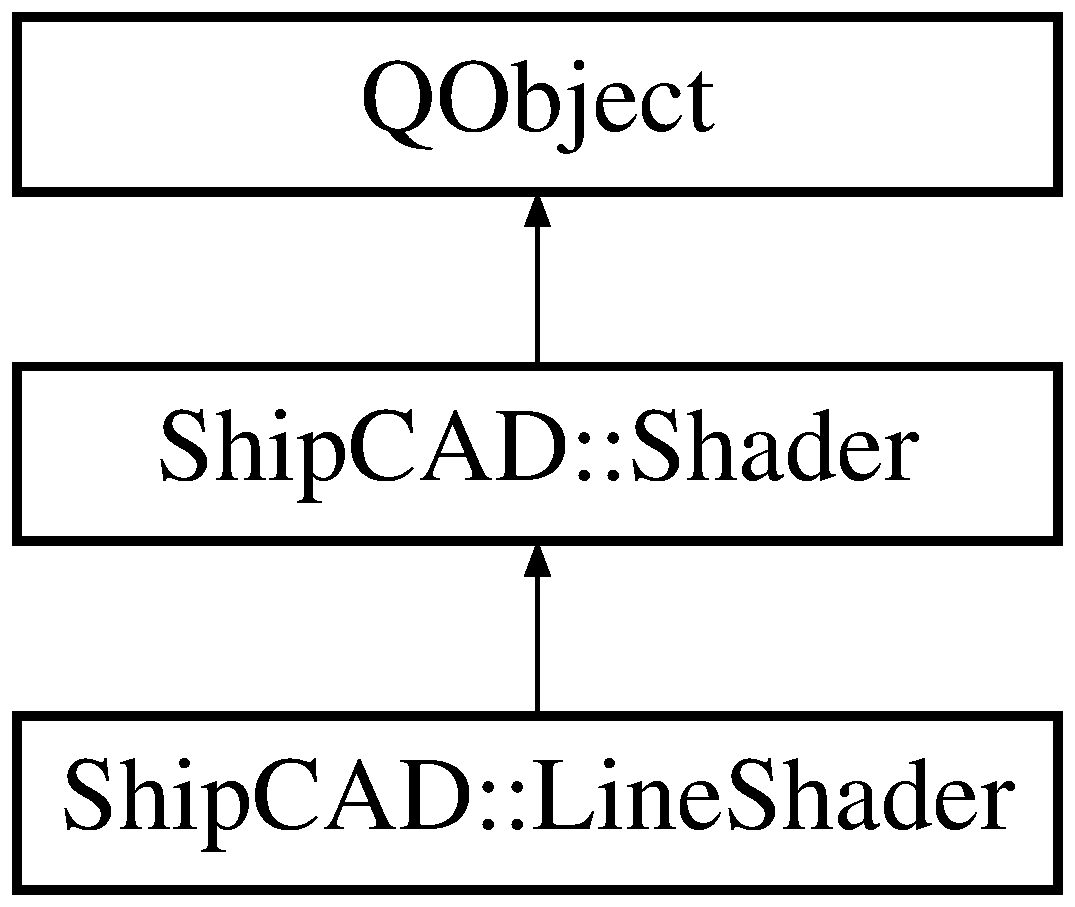
\includegraphics[height=3.000000cm]{classShipCAD_1_1LineShader}
\end{center}
\end{figure}
\subsection*{Public Member Functions}
\begin{DoxyCompactItemize}
\item 
\hyperlink{classShipCAD_1_1LineShader_ae06ecf68dfc054511db3937893850d2f}{Line\-Shader} (\hyperlink{classShipCAD_1_1Viewport}{Viewport} $\ast$vp)
\item 
virtual \hyperlink{classShipCAD_1_1LineShader_ae5c2761813aac4839a5b31648e37d343}{$\sim$\-Line\-Shader} ()
\item 
void \hyperlink{classShipCAD_1_1LineShader_aaa105117e559ec413a733e14dc638b5a}{render\-Points} (Q\-Vector$<$ Q\-Vector3\-D $>$ \&points, Q\-Color color)
\item 
void \hyperlink{classShipCAD_1_1LineShader_a3d30bda1883e0eda65ea23c4da76f610}{render\-Lines} (Q\-Vector$<$ Q\-Vector3\-D $>$ \&vertices, Q\-Color line\-Color)
\end{DoxyCompactItemize}
\subsection*{Additional Inherited Members}


\subsection{Detailed Description}


Definition at line 77 of file shader.\-h.



\subsection{Constructor \& Destructor Documentation}
\hypertarget{classShipCAD_1_1LineShader_ae06ecf68dfc054511db3937893850d2f}{\index{Ship\-C\-A\-D\-::\-Line\-Shader@{Ship\-C\-A\-D\-::\-Line\-Shader}!Line\-Shader@{Line\-Shader}}
\index{Line\-Shader@{Line\-Shader}!ShipCAD::LineShader@{Ship\-C\-A\-D\-::\-Line\-Shader}}
\subsubsection[{Line\-Shader}]{\setlength{\rightskip}{0pt plus 5cm}Line\-Shader\-::\-Line\-Shader (
\begin{DoxyParamCaption}
\item[{{\bf Viewport} $\ast$}]{vp}
\end{DoxyParamCaption}
)\hspace{0.3cm}{\ttfamily [explicit]}}}\label{classShipCAD_1_1LineShader_ae06ecf68dfc054511db3937893850d2f}


Definition at line 110 of file shader.\-cpp.

\hypertarget{classShipCAD_1_1LineShader_ae5c2761813aac4839a5b31648e37d343}{\index{Ship\-C\-A\-D\-::\-Line\-Shader@{Ship\-C\-A\-D\-::\-Line\-Shader}!$\sim$\-Line\-Shader@{$\sim$\-Line\-Shader}}
\index{$\sim$\-Line\-Shader@{$\sim$\-Line\-Shader}!ShipCAD::LineShader@{Ship\-C\-A\-D\-::\-Line\-Shader}}
\subsubsection[{$\sim$\-Line\-Shader}]{\setlength{\rightskip}{0pt plus 5cm}virtual Ship\-C\-A\-D\-::\-Line\-Shader\-::$\sim$\-Line\-Shader (
\begin{DoxyParamCaption}
{}
\end{DoxyParamCaption}
)\hspace{0.3cm}{\ttfamily [inline]}, {\ttfamily [virtual]}}}\label{classShipCAD_1_1LineShader_ae5c2761813aac4839a5b31648e37d343}


Definition at line 84 of file shader.\-h.



\subsection{Member Function Documentation}
\hypertarget{classShipCAD_1_1LineShader_a3d30bda1883e0eda65ea23c4da76f610}{\index{Ship\-C\-A\-D\-::\-Line\-Shader@{Ship\-C\-A\-D\-::\-Line\-Shader}!render\-Lines@{render\-Lines}}
\index{render\-Lines@{render\-Lines}!ShipCAD::LineShader@{Ship\-C\-A\-D\-::\-Line\-Shader}}
\subsubsection[{render\-Lines}]{\setlength{\rightskip}{0pt plus 5cm}void Line\-Shader\-::render\-Lines (
\begin{DoxyParamCaption}
\item[{Q\-Vector$<$ Q\-Vector3\-D $>$ \&}]{vertices, }
\item[{Q\-Color}]{line\-Color}
\end{DoxyParamCaption}
)}}\label{classShipCAD_1_1LineShader_a3d30bda1883e0eda65ea23c4da76f610}


Definition at line 136 of file shader.\-cpp.

\hypertarget{classShipCAD_1_1LineShader_aaa105117e559ec413a733e14dc638b5a}{\index{Ship\-C\-A\-D\-::\-Line\-Shader@{Ship\-C\-A\-D\-::\-Line\-Shader}!render\-Points@{render\-Points}}
\index{render\-Points@{render\-Points}!ShipCAD::LineShader@{Ship\-C\-A\-D\-::\-Line\-Shader}}
\subsubsection[{render\-Points}]{\setlength{\rightskip}{0pt plus 5cm}void Line\-Shader\-::render\-Points (
\begin{DoxyParamCaption}
\item[{Q\-Vector$<$ Q\-Vector3\-D $>$ \&}]{points, }
\item[{Q\-Color}]{color}
\end{DoxyParamCaption}
)}}\label{classShipCAD_1_1LineShader_aaa105117e559ec413a733e14dc638b5a}


Definition at line 120 of file shader.\-cpp.



The documentation for this class was generated from the following files\-:\begin{DoxyCompactItemize}
\item 
Ship\-C\-A\-Dlib/\hyperlink{shader_8h}{shader.\-h}\item 
Ship\-C\-A\-Dlib/\hyperlink{shader_8cpp}{shader.\-cpp}\end{DoxyCompactItemize}

\hypertarget{classShipCAD_1_1ListIndexOutOfBounds}{\section{Ship\-C\-A\-D\-:\-:List\-Index\-Out\-Of\-Bounds Class Reference}
\label{classShipCAD_1_1ListIndexOutOfBounds}\index{Ship\-C\-A\-D\-::\-List\-Index\-Out\-Of\-Bounds@{Ship\-C\-A\-D\-::\-List\-Index\-Out\-Of\-Bounds}}
}


{\ttfamily \#include $<$exception.\-h$>$}

Inheritance diagram for Ship\-C\-A\-D\-:\-:List\-Index\-Out\-Of\-Bounds\-:\begin{figure}[H]
\begin{center}
\leavevmode
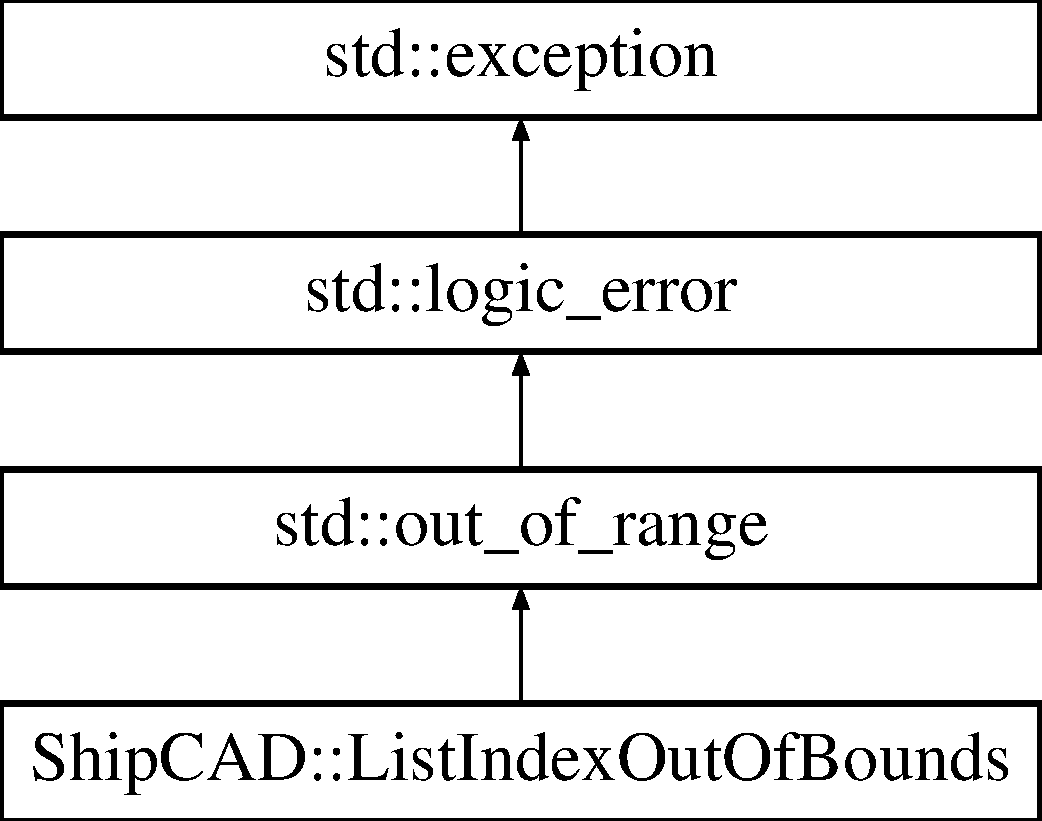
\includegraphics[height=4.000000cm]{classShipCAD_1_1ListIndexOutOfBounds}
\end{center}
\end{figure}
\subsection*{Public Member Functions}
\begin{DoxyCompactItemize}
\item 
\hyperlink{classShipCAD_1_1ListIndexOutOfBounds_a99a4a2511ef6f802cbcf7d4ccd8c6453}{List\-Index\-Out\-Of\-Bounds} (const std\-::string \&what\-\_\-arg)
\end{DoxyCompactItemize}


\subsection{Detailed Description}


Definition at line 38 of file exception.\-h.



\subsection{Constructor \& Destructor Documentation}
\hypertarget{classShipCAD_1_1ListIndexOutOfBounds_a99a4a2511ef6f802cbcf7d4ccd8c6453}{\index{Ship\-C\-A\-D\-::\-List\-Index\-Out\-Of\-Bounds@{Ship\-C\-A\-D\-::\-List\-Index\-Out\-Of\-Bounds}!List\-Index\-Out\-Of\-Bounds@{List\-Index\-Out\-Of\-Bounds}}
\index{List\-Index\-Out\-Of\-Bounds@{List\-Index\-Out\-Of\-Bounds}!ShipCAD::ListIndexOutOfBounds@{Ship\-C\-A\-D\-::\-List\-Index\-Out\-Of\-Bounds}}
\subsubsection[{List\-Index\-Out\-Of\-Bounds}]{\setlength{\rightskip}{0pt plus 5cm}Ship\-C\-A\-D\-::\-List\-Index\-Out\-Of\-Bounds\-::\-List\-Index\-Out\-Of\-Bounds (
\begin{DoxyParamCaption}
\item[{const std\-::string \&}]{what\-\_\-arg}
\end{DoxyParamCaption}
)\hspace{0.3cm}{\ttfamily [inline]}}}\label{classShipCAD_1_1ListIndexOutOfBounds_a99a4a2511ef6f802cbcf7d4ccd8c6453}


Definition at line 41 of file exception.\-h.



The documentation for this class was generated from the following file\-:\begin{DoxyCompactItemize}
\item 
Ship\-C\-A\-Dlib/\hyperlink{exception_8h}{exception.\-h}\end{DoxyCompactItemize}

\hypertarget{classMainWindow}{\section{Main\-Window Class Reference}
\label{classMainWindow}\index{Main\-Window@{Main\-Window}}
}


{\ttfamily \#include $<$mainwindow.\-h$>$}

Inheritance diagram for Main\-Window\-:\begin{figure}[H]
\begin{center}
\leavevmode
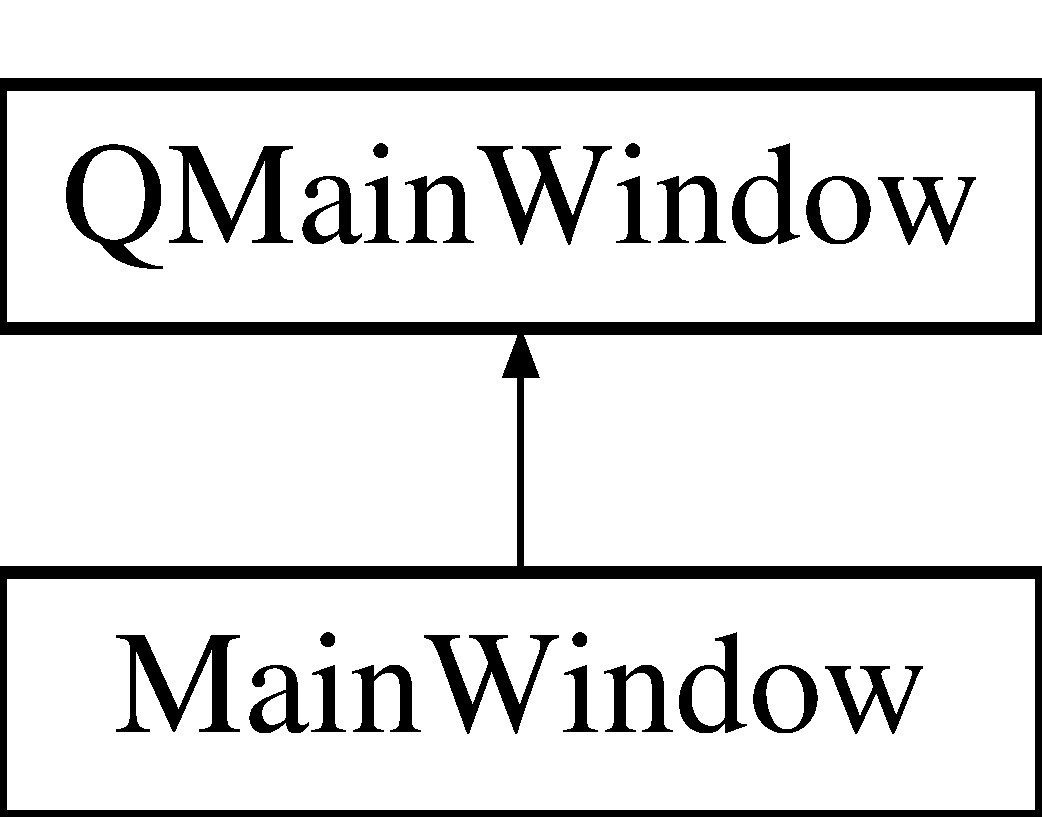
\includegraphics[height=2.000000cm]{classMainWindow}
\end{center}
\end{figure}
\subsection*{Public Slots}
\begin{DoxyCompactItemize}
\item 
void \hyperlink{classMainWindow_a288b768c3c21a9171bdc56fe845ece8b}{open\-File} ()
\end{DoxyCompactItemize}
\subsection*{Public Member Functions}
\begin{DoxyCompactItemize}
\item 
\hyperlink{classMainWindow_a8b244be8b7b7db1b08de2a2acb9409db}{Main\-Window} (Q\-Widget $\ast$parent=0)
\item 
\hyperlink{classMainWindow_ae98d00a93bc118200eeef9f9bba1dba7}{$\sim$\-Main\-Window} ()
\item 
void \hyperlink{classMainWindow_ae53d70703200d86162a68a9a8ba593ee}{set\-Animating} (bool animating)
\item 
void \hyperlink{classMainWindow_a09cb0428e2c3a4226c04eafff3904f5d}{set\-Surface} (\hyperlink{classShipCAD_1_1SubdivisionSurface}{Ship\-C\-A\-D\-::\-Subdivision\-Surface} $\ast$surface)
\end{DoxyCompactItemize}
\subsection*{Protected Slots}
\begin{DoxyCompactItemize}
\item 
void \hyperlink{classMainWindow_a8690702fe505fb6786ae98f9cad71118}{wire\-Frame} ()
\item 
void \hyperlink{classMainWindow_ad2040b40c2d18b4dea61d33699ae0a90}{shade} ()
\item 
void \hyperlink{classMainWindow_af7f1931b45432a43105345f806097501}{shade\-Curvature} ()
\item 
void \hyperlink{classMainWindow_a7827c32592a7991f37e87f2ba94b3ccd}{shade\-Developable} ()
\item 
void \hyperlink{classMainWindow_afc072912649b8cc513963db3b2f05283}{shade\-Zebra} ()
\item 
void \hyperlink{classMainWindow_a93b8868bdce207842de4747008f5e03e}{show\-Control\-Net} (bool val)
\item 
void \hyperlink{classMainWindow_aa0401a2a6241ff56390b1825f4e0e508}{show\-Interior\-Edges} (bool val)
\item 
void \hyperlink{classMainWindow_ac7ec359ed2a0f3c66ba5d2a788613832}{show\-Control\-Curves} (bool val)
\item 
void \hyperlink{classMainWindow_a65462f395b206a9a680a5521082b6344}{show\-Curvature} (bool val)
\item 
void \hyperlink{classMainWindow_a8edd7fa619d2ed66b94f6a498f5af59c}{show\-Normals} (bool val)
\item 
void \hyperlink{classMainWindow_afb7953f1fdcb7c5a77efa6fb4d2c3cd5}{draw\-Mirror} (bool val)
\item 
void \hyperlink{classMainWindow_adecb2e29c0d3df68517a570dc9e352bd}{shade\-Underwater} (bool val)
\item 
void \hyperlink{classMainWindow_a4a399825baba544bf4850e06e5e1fa94}{animation\-Timeout} ()
\end{DoxyCompactItemize}


\subsection{Detailed Description}


Definition at line 45 of file mainwindow.\-h.



\subsection{Constructor \& Destructor Documentation}
\hypertarget{classMainWindow_a8b244be8b7b7db1b08de2a2acb9409db}{\index{Main\-Window@{Main\-Window}!Main\-Window@{Main\-Window}}
\index{Main\-Window@{Main\-Window}!MainWindow@{Main\-Window}}
\subsubsection[{Main\-Window}]{\setlength{\rightskip}{0pt plus 5cm}Main\-Window\-::\-Main\-Window (
\begin{DoxyParamCaption}
\item[{Q\-Widget $\ast$}]{parent = {\ttfamily 0}}
\end{DoxyParamCaption}
)\hspace{0.3cm}{\ttfamily [explicit]}}}\label{classMainWindow_a8b244be8b7b7db1b08de2a2acb9409db}


Definition at line 48 of file mainwindow.\-cpp.

\hypertarget{classMainWindow_ae98d00a93bc118200eeef9f9bba1dba7}{\index{Main\-Window@{Main\-Window}!$\sim$\-Main\-Window@{$\sim$\-Main\-Window}}
\index{$\sim$\-Main\-Window@{$\sim$\-Main\-Window}!MainWindow@{Main\-Window}}
\subsubsection[{$\sim$\-Main\-Window}]{\setlength{\rightskip}{0pt plus 5cm}Main\-Window\-::$\sim$\-Main\-Window (
\begin{DoxyParamCaption}
{}
\end{DoxyParamCaption}
)}}\label{classMainWindow_ae98d00a93bc118200eeef9f9bba1dba7}


Definition at line 159 of file mainwindow.\-cpp.



\subsection{Member Function Documentation}
\hypertarget{classMainWindow_a4a399825baba544bf4850e06e5e1fa94}{\index{Main\-Window@{Main\-Window}!animation\-Timeout@{animation\-Timeout}}
\index{animation\-Timeout@{animation\-Timeout}!MainWindow@{Main\-Window}}
\subsubsection[{animation\-Timeout}]{\setlength{\rightskip}{0pt plus 5cm}void Main\-Window\-::animation\-Timeout (
\begin{DoxyParamCaption}
{}
\end{DoxyParamCaption}
)\hspace{0.3cm}{\ttfamily [protected]}, {\ttfamily [slot]}}}\label{classMainWindow_a4a399825baba544bf4850e06e5e1fa94}


Definition at line 186 of file mainwindow.\-cpp.

\hypertarget{classMainWindow_afb7953f1fdcb7c5a77efa6fb4d2c3cd5}{\index{Main\-Window@{Main\-Window}!draw\-Mirror@{draw\-Mirror}}
\index{draw\-Mirror@{draw\-Mirror}!MainWindow@{Main\-Window}}
\subsubsection[{draw\-Mirror}]{\setlength{\rightskip}{0pt plus 5cm}void Main\-Window\-::draw\-Mirror (
\begin{DoxyParamCaption}
\item[{bool}]{val}
\end{DoxyParamCaption}
)\hspace{0.3cm}{\ttfamily [protected]}, {\ttfamily [slot]}}}\label{classMainWindow_afb7953f1fdcb7c5a77efa6fb4d2c3cd5}


Definition at line 360 of file mainwindow.\-cpp.

\hypertarget{classMainWindow_a288b768c3c21a9171bdc56fe845ece8b}{\index{Main\-Window@{Main\-Window}!open\-File@{open\-File}}
\index{open\-File@{open\-File}!MainWindow@{Main\-Window}}
\subsubsection[{open\-File}]{\setlength{\rightskip}{0pt plus 5cm}void Main\-Window\-::open\-File (
\begin{DoxyParamCaption}
{}
\end{DoxyParamCaption}
)\hspace{0.3cm}{\ttfamily [slot]}}}\label{classMainWindow_a288b768c3c21a9171bdc56fe845ece8b}


Definition at line 211 of file mainwindow.\-cpp.

\hypertarget{classMainWindow_ae53d70703200d86162a68a9a8ba593ee}{\index{Main\-Window@{Main\-Window}!set\-Animating@{set\-Animating}}
\index{set\-Animating@{set\-Animating}!MainWindow@{Main\-Window}}
\subsubsection[{set\-Animating}]{\setlength{\rightskip}{0pt plus 5cm}void Main\-Window\-::set\-Animating (
\begin{DoxyParamCaption}
\item[{bool}]{animating}
\end{DoxyParamCaption}
)}}\label{classMainWindow_ae53d70703200d86162a68a9a8ba593ee}


Definition at line 167 of file mainwindow.\-cpp.

\hypertarget{classMainWindow_a09cb0428e2c3a4226c04eafff3904f5d}{\index{Main\-Window@{Main\-Window}!set\-Surface@{set\-Surface}}
\index{set\-Surface@{set\-Surface}!MainWindow@{Main\-Window}}
\subsubsection[{set\-Surface}]{\setlength{\rightskip}{0pt plus 5cm}void Main\-Window\-::set\-Surface (
\begin{DoxyParamCaption}
\item[{{\bf Ship\-C\-A\-D\-::\-Subdivision\-Surface} $\ast$}]{surface}
\end{DoxyParamCaption}
)}}\label{classMainWindow_a09cb0428e2c3a4226c04eafff3904f5d}


Definition at line 250 of file mainwindow.\-cpp.

\hypertarget{classMainWindow_ad2040b40c2d18b4dea61d33699ae0a90}{\index{Main\-Window@{Main\-Window}!shade@{shade}}
\index{shade@{shade}!MainWindow@{Main\-Window}}
\subsubsection[{shade}]{\setlength{\rightskip}{0pt plus 5cm}void Main\-Window\-::shade (
\begin{DoxyParamCaption}
{}
\end{DoxyParamCaption}
)\hspace{0.3cm}{\ttfamily [protected]}, {\ttfamily [slot]}}}\label{classMainWindow_ad2040b40c2d18b4dea61d33699ae0a90}


Definition at line 273 of file mainwindow.\-cpp.

\hypertarget{classMainWindow_af7f1931b45432a43105345f806097501}{\index{Main\-Window@{Main\-Window}!shade\-Curvature@{shade\-Curvature}}
\index{shade\-Curvature@{shade\-Curvature}!MainWindow@{Main\-Window}}
\subsubsection[{shade\-Curvature}]{\setlength{\rightskip}{0pt plus 5cm}void Main\-Window\-::shade\-Curvature (
\begin{DoxyParamCaption}
{}
\end{DoxyParamCaption}
)\hspace{0.3cm}{\ttfamily [protected]}, {\ttfamily [slot]}}}\label{classMainWindow_af7f1931b45432a43105345f806097501}


Definition at line 281 of file mainwindow.\-cpp.

\hypertarget{classMainWindow_a7827c32592a7991f37e87f2ba94b3ccd}{\index{Main\-Window@{Main\-Window}!shade\-Developable@{shade\-Developable}}
\index{shade\-Developable@{shade\-Developable}!MainWindow@{Main\-Window}}
\subsubsection[{shade\-Developable}]{\setlength{\rightskip}{0pt plus 5cm}void Main\-Window\-::shade\-Developable (
\begin{DoxyParamCaption}
{}
\end{DoxyParamCaption}
)\hspace{0.3cm}{\ttfamily [protected]}, {\ttfamily [slot]}}}\label{classMainWindow_a7827c32592a7991f37e87f2ba94b3ccd}


Definition at line 289 of file mainwindow.\-cpp.

\hypertarget{classMainWindow_adecb2e29c0d3df68517a570dc9e352bd}{\index{Main\-Window@{Main\-Window}!shade\-Underwater@{shade\-Underwater}}
\index{shade\-Underwater@{shade\-Underwater}!MainWindow@{Main\-Window}}
\subsubsection[{shade\-Underwater}]{\setlength{\rightskip}{0pt plus 5cm}void Main\-Window\-::shade\-Underwater (
\begin{DoxyParamCaption}
\item[{bool}]{val}
\end{DoxyParamCaption}
)\hspace{0.3cm}{\ttfamily [protected]}, {\ttfamily [slot]}}}\label{classMainWindow_adecb2e29c0d3df68517a570dc9e352bd}


Definition at line 371 of file mainwindow.\-cpp.

\hypertarget{classMainWindow_afc072912649b8cc513963db3b2f05283}{\index{Main\-Window@{Main\-Window}!shade\-Zebra@{shade\-Zebra}}
\index{shade\-Zebra@{shade\-Zebra}!MainWindow@{Main\-Window}}
\subsubsection[{shade\-Zebra}]{\setlength{\rightskip}{0pt plus 5cm}void Main\-Window\-::shade\-Zebra (
\begin{DoxyParamCaption}
{}
\end{DoxyParamCaption}
)\hspace{0.3cm}{\ttfamily [protected]}, {\ttfamily [slot]}}}\label{classMainWindow_afc072912649b8cc513963db3b2f05283}


Definition at line 297 of file mainwindow.\-cpp.

\hypertarget{classMainWindow_ac7ec359ed2a0f3c66ba5d2a788613832}{\index{Main\-Window@{Main\-Window}!show\-Control\-Curves@{show\-Control\-Curves}}
\index{show\-Control\-Curves@{show\-Control\-Curves}!MainWindow@{Main\-Window}}
\subsubsection[{show\-Control\-Curves}]{\setlength{\rightskip}{0pt plus 5cm}void Main\-Window\-::show\-Control\-Curves (
\begin{DoxyParamCaption}
\item[{bool}]{val}
\end{DoxyParamCaption}
)\hspace{0.3cm}{\ttfamily [protected]}, {\ttfamily [slot]}}}\label{classMainWindow_ac7ec359ed2a0f3c66ba5d2a788613832}


Definition at line 327 of file mainwindow.\-cpp.

\hypertarget{classMainWindow_a93b8868bdce207842de4747008f5e03e}{\index{Main\-Window@{Main\-Window}!show\-Control\-Net@{show\-Control\-Net}}
\index{show\-Control\-Net@{show\-Control\-Net}!MainWindow@{Main\-Window}}
\subsubsection[{show\-Control\-Net}]{\setlength{\rightskip}{0pt plus 5cm}void Main\-Window\-::show\-Control\-Net (
\begin{DoxyParamCaption}
\item[{bool}]{val}
\end{DoxyParamCaption}
)\hspace{0.3cm}{\ttfamily [protected]}, {\ttfamily [slot]}}}\label{classMainWindow_a93b8868bdce207842de4747008f5e03e}


Definition at line 305 of file mainwindow.\-cpp.

\hypertarget{classMainWindow_a65462f395b206a9a680a5521082b6344}{\index{Main\-Window@{Main\-Window}!show\-Curvature@{show\-Curvature}}
\index{show\-Curvature@{show\-Curvature}!MainWindow@{Main\-Window}}
\subsubsection[{show\-Curvature}]{\setlength{\rightskip}{0pt plus 5cm}void Main\-Window\-::show\-Curvature (
\begin{DoxyParamCaption}
\item[{bool}]{val}
\end{DoxyParamCaption}
)\hspace{0.3cm}{\ttfamily [protected]}, {\ttfamily [slot]}}}\label{classMainWindow_a65462f395b206a9a680a5521082b6344}


Definition at line 338 of file mainwindow.\-cpp.

\hypertarget{classMainWindow_aa0401a2a6241ff56390b1825f4e0e508}{\index{Main\-Window@{Main\-Window}!show\-Interior\-Edges@{show\-Interior\-Edges}}
\index{show\-Interior\-Edges@{show\-Interior\-Edges}!MainWindow@{Main\-Window}}
\subsubsection[{show\-Interior\-Edges}]{\setlength{\rightskip}{0pt plus 5cm}void Main\-Window\-::show\-Interior\-Edges (
\begin{DoxyParamCaption}
\item[{bool}]{val}
\end{DoxyParamCaption}
)\hspace{0.3cm}{\ttfamily [protected]}, {\ttfamily [slot]}}}\label{classMainWindow_aa0401a2a6241ff56390b1825f4e0e508}


Definition at line 316 of file mainwindow.\-cpp.

\hypertarget{classMainWindow_a8edd7fa619d2ed66b94f6a498f5af59c}{\index{Main\-Window@{Main\-Window}!show\-Normals@{show\-Normals}}
\index{show\-Normals@{show\-Normals}!MainWindow@{Main\-Window}}
\subsubsection[{show\-Normals}]{\setlength{\rightskip}{0pt plus 5cm}void Main\-Window\-::show\-Normals (
\begin{DoxyParamCaption}
\item[{bool}]{val}
\end{DoxyParamCaption}
)\hspace{0.3cm}{\ttfamily [protected]}, {\ttfamily [slot]}}}\label{classMainWindow_a8edd7fa619d2ed66b94f6a498f5af59c}


Definition at line 349 of file mainwindow.\-cpp.

\hypertarget{classMainWindow_a8690702fe505fb6786ae98f9cad71118}{\index{Main\-Window@{Main\-Window}!wire\-Frame@{wire\-Frame}}
\index{wire\-Frame@{wire\-Frame}!MainWindow@{Main\-Window}}
\subsubsection[{wire\-Frame}]{\setlength{\rightskip}{0pt plus 5cm}void Main\-Window\-::wire\-Frame (
\begin{DoxyParamCaption}
{}
\end{DoxyParamCaption}
)\hspace{0.3cm}{\ttfamily [protected]}, {\ttfamily [slot]}}}\label{classMainWindow_a8690702fe505fb6786ae98f9cad71118}


Definition at line 265 of file mainwindow.\-cpp.



The documentation for this class was generated from the following files\-:\begin{DoxyCompactItemize}
\item 
Viewer/\hyperlink{mainwindow_8h}{mainwindow.\-h}\item 
Viewer/\hyperlink{mainwindow_8cpp}{mainwindow.\-cpp}\end{DoxyCompactItemize}

\hypertarget{classShipCAD_1_1Marker}{\section{Ship\-C\-A\-D\-:\-:Marker Class Reference}
\label{classShipCAD_1_1Marker}\index{Ship\-C\-A\-D\-::\-Marker@{Ship\-C\-A\-D\-::\-Marker}}
}


{\ttfamily \#include $<$marker.\-h$>$}

Inheritance diagram for Ship\-C\-A\-D\-:\-:Marker\-:\begin{figure}[H]
\begin{center}
\leavevmode
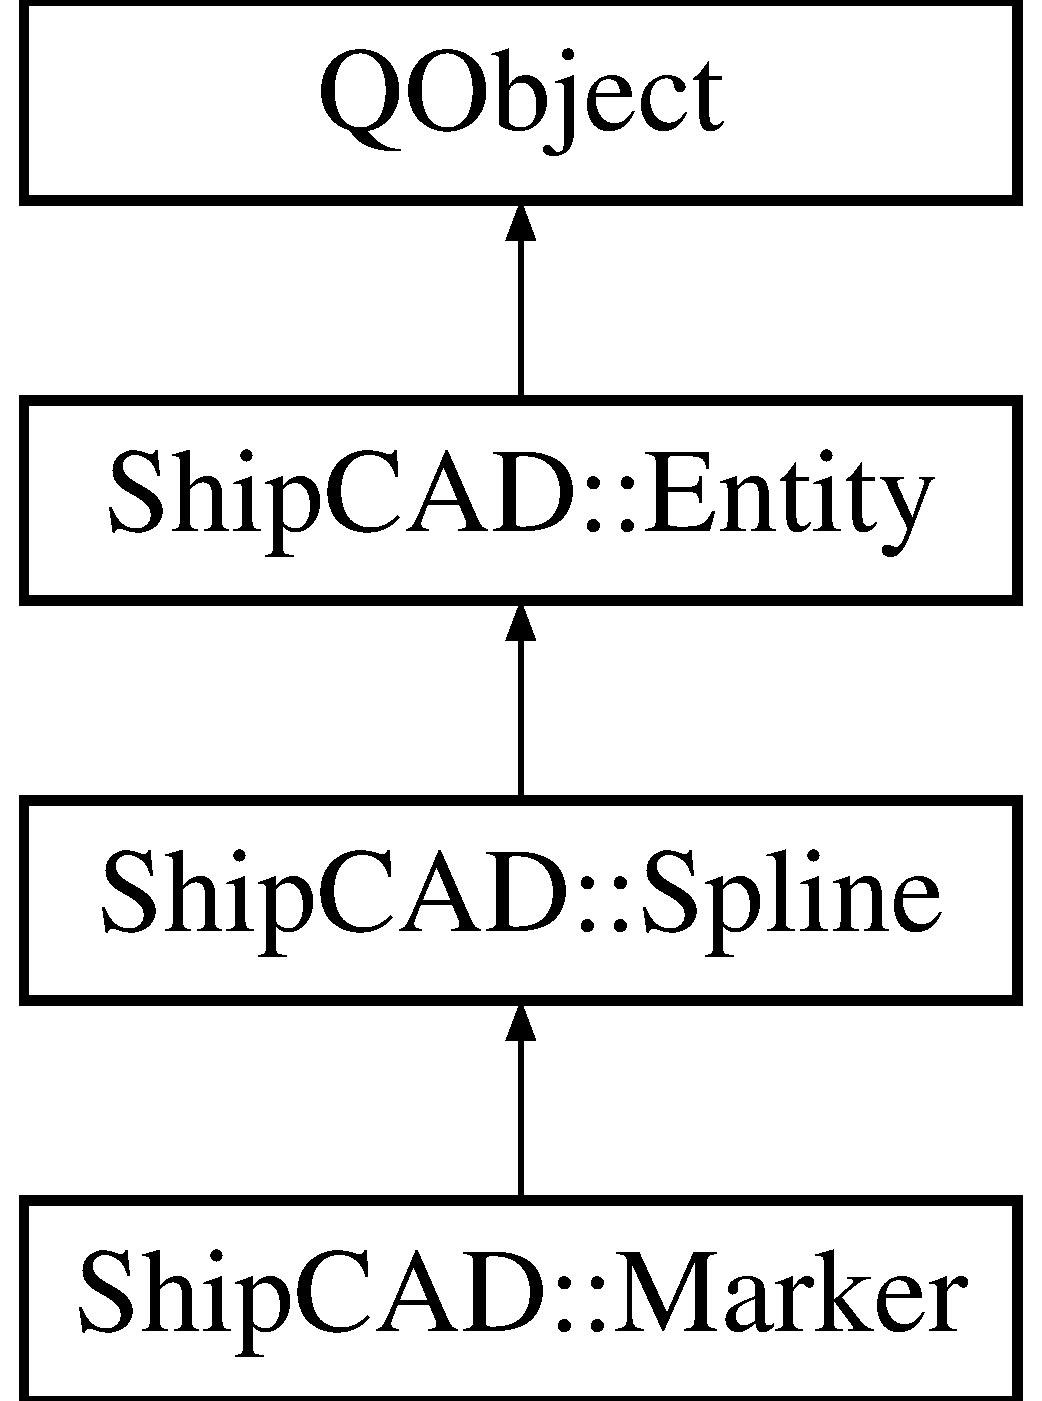
\includegraphics[height=4.000000cm]{classShipCAD_1_1Marker}
\end{center}
\end{figure}
\subsection*{Public Member Functions}
\begin{DoxyCompactItemize}
\item 
\hyperlink{classShipCAD_1_1Marker_a216cf592a0945f6b6923a00c9625e3bf}{Marker} (\hyperlink{classShipCAD_1_1ShipCADModel}{Ship\-C\-A\-D\-Model} $\ast$owner)
\item 
virtual \hyperlink{classShipCAD_1_1Marker_a2f3196a90d442386b0d50f54b69e6116}{$\sim$\-Marker} ()
\item 
virtual void \hyperlink{classShipCAD_1_1Marker_ac7c7eea8648562f3fa00a9e10af6ec97}{clear} ()
\item 
virtual void \hyperlink{classShipCAD_1_1Marker_a0cca647d9b32dc69b03903b024dc3091}{draw} (\hyperlink{classShipCAD_1_1Viewport}{Viewport} \&vp, \hyperlink{classShipCAD_1_1LineShader}{Line\-Shader} $\ast$lineshader)
\item 
bool \hyperlink{classShipCAD_1_1Marker_a693fef3930809d5c4b2ce3755662e367}{is\-Visible} ()
\item 
void \hyperlink{classShipCAD_1_1Marker_af21b0bac028e01ce02ea97bf6f83cccc}{set\-Visible} (bool set)
\item 
bool \hyperlink{classShipCAD_1_1Marker_aac6bc8a781945739646cfc8dd6c5b99c}{is\-Selected} ()
\item 
void \hyperlink{classShipCAD_1_1Marker_ad3bbb4a01e11e3d2885f56599a77a3d1}{set\-Selected} (bool set)
\item 
void \hyperlink{classShipCAD_1_1Marker_a0f2aa7cd6bae40784c077b89d5ebdb50}{load\-Binary} (\hyperlink{classShipCAD_1_1FileBuffer}{File\-Buffer} \&source)
\item 
void \hyperlink{classShipCAD_1_1Marker_abceb4cbb5b038eb88d0f7f26507be15c}{save\-Binary} (\hyperlink{classShipCAD_1_1FileBuffer}{File\-Buffer} \&dest)
\end{DoxyCompactItemize}
\subsection*{Static Public Member Functions}
\begin{DoxyCompactItemize}
\item 
static \hyperlink{classShipCAD_1_1Marker}{Marker} $\ast$ \hyperlink{classShipCAD_1_1Marker_af505b0f8f0aa9049fd65a7f9b675abbc}{construct} (\hyperlink{classShipCAD_1_1ShipCADModel}{Ship\-C\-A\-D\-Model} $\ast$owner)
\end{DoxyCompactItemize}
\subsection*{Additional Inherited Members}


\subsection{Detailed Description}


Definition at line 48 of file marker.\-h.



\subsection{Constructor \& Destructor Documentation}
\hypertarget{classShipCAD_1_1Marker_a216cf592a0945f6b6923a00c9625e3bf}{\index{Ship\-C\-A\-D\-::\-Marker@{Ship\-C\-A\-D\-::\-Marker}!Marker@{Marker}}
\index{Marker@{Marker}!ShipCAD::Marker@{Ship\-C\-A\-D\-::\-Marker}}
\subsubsection[{Marker}]{\setlength{\rightskip}{0pt plus 5cm}Marker\-::\-Marker (
\begin{DoxyParamCaption}
\item[{{\bf Ship\-C\-A\-D\-Model} $\ast$}]{owner}
\end{DoxyParamCaption}
)\hspace{0.3cm}{\ttfamily [explicit]}}}\label{classShipCAD_1_1Marker_a216cf592a0945f6b6923a00c9625e3bf}


Definition at line 45 of file marker.\-cpp.

\hypertarget{classShipCAD_1_1Marker_a2f3196a90d442386b0d50f54b69e6116}{\index{Ship\-C\-A\-D\-::\-Marker@{Ship\-C\-A\-D\-::\-Marker}!$\sim$\-Marker@{$\sim$\-Marker}}
\index{$\sim$\-Marker@{$\sim$\-Marker}!ShipCAD::Marker@{Ship\-C\-A\-D\-::\-Marker}}
\subsubsection[{$\sim$\-Marker}]{\setlength{\rightskip}{0pt plus 5cm}virtual Ship\-C\-A\-D\-::\-Marker\-::$\sim$\-Marker (
\begin{DoxyParamCaption}
{}
\end{DoxyParamCaption}
)\hspace{0.3cm}{\ttfamily [inline]}, {\ttfamily [virtual]}}}\label{classShipCAD_1_1Marker_a2f3196a90d442386b0d50f54b69e6116}


Definition at line 55 of file marker.\-h.



\subsection{Member Function Documentation}
\hypertarget{classShipCAD_1_1Marker_ac7c7eea8648562f3fa00a9e10af6ec97}{\index{Ship\-C\-A\-D\-::\-Marker@{Ship\-C\-A\-D\-::\-Marker}!clear@{clear}}
\index{clear@{clear}!ShipCAD::Marker@{Ship\-C\-A\-D\-::\-Marker}}
\subsubsection[{clear}]{\setlength{\rightskip}{0pt plus 5cm}void Marker\-::clear (
\begin{DoxyParamCaption}
{}
\end{DoxyParamCaption}
)\hspace{0.3cm}{\ttfamily [virtual]}}}\label{classShipCAD_1_1Marker_ac7c7eea8648562f3fa00a9e10af6ec97}


Reimplemented from \hyperlink{classShipCAD_1_1Spline_a02967f3eee8b1755eab0d7da55c3c621}{Ship\-C\-A\-D\-::\-Spline}.



Definition at line 57 of file marker.\-cpp.

\hypertarget{classShipCAD_1_1Marker_af505b0f8f0aa9049fd65a7f9b675abbc}{\index{Ship\-C\-A\-D\-::\-Marker@{Ship\-C\-A\-D\-::\-Marker}!construct@{construct}}
\index{construct@{construct}!ShipCAD::Marker@{Ship\-C\-A\-D\-::\-Marker}}
\subsubsection[{construct}]{\setlength{\rightskip}{0pt plus 5cm}{\bf Marker} $\ast$ Marker\-::construct (
\begin{DoxyParamCaption}
\item[{{\bf Ship\-C\-A\-D\-Model} $\ast$}]{owner}
\end{DoxyParamCaption}
)\hspace{0.3cm}{\ttfamily [static]}}}\label{classShipCAD_1_1Marker_af505b0f8f0aa9049fd65a7f9b675abbc}


Definition at line 51 of file marker.\-cpp.

\hypertarget{classShipCAD_1_1Marker_a0cca647d9b32dc69b03903b024dc3091}{\index{Ship\-C\-A\-D\-::\-Marker@{Ship\-C\-A\-D\-::\-Marker}!draw@{draw}}
\index{draw@{draw}!ShipCAD::Marker@{Ship\-C\-A\-D\-::\-Marker}}
\subsubsection[{draw}]{\setlength{\rightskip}{0pt plus 5cm}void Marker\-::draw (
\begin{DoxyParamCaption}
\item[{{\bf Viewport} \&}]{vp, }
\item[{{\bf Line\-Shader} $\ast$}]{lineshader}
\end{DoxyParamCaption}
)\hspace{0.3cm}{\ttfamily [virtual]}}}\label{classShipCAD_1_1Marker_a0cca647d9b32dc69b03903b024dc3091}


Reimplemented from \hyperlink{classShipCAD_1_1Spline_a6424ed433d241f566c15891cc25a74dd}{Ship\-C\-A\-D\-::\-Spline}.



Definition at line 63 of file marker.\-cpp.

\hypertarget{classShipCAD_1_1Marker_aac6bc8a781945739646cfc8dd6c5b99c}{\index{Ship\-C\-A\-D\-::\-Marker@{Ship\-C\-A\-D\-::\-Marker}!is\-Selected@{is\-Selected}}
\index{is\-Selected@{is\-Selected}!ShipCAD::Marker@{Ship\-C\-A\-D\-::\-Marker}}
\subsubsection[{is\-Selected}]{\setlength{\rightskip}{0pt plus 5cm}bool Marker\-::is\-Selected (
\begin{DoxyParamCaption}
{}
\end{DoxyParamCaption}
)}}\label{classShipCAD_1_1Marker_aac6bc8a781945739646cfc8dd6c5b99c}


Definition at line 68 of file marker.\-cpp.

\hypertarget{classShipCAD_1_1Marker_a693fef3930809d5c4b2ce3755662e367}{\index{Ship\-C\-A\-D\-::\-Marker@{Ship\-C\-A\-D\-::\-Marker}!is\-Visible@{is\-Visible}}
\index{is\-Visible@{is\-Visible}!ShipCAD::Marker@{Ship\-C\-A\-D\-::\-Marker}}
\subsubsection[{is\-Visible}]{\setlength{\rightskip}{0pt plus 5cm}bool Ship\-C\-A\-D\-::\-Marker\-::is\-Visible (
\begin{DoxyParamCaption}
{}
\end{DoxyParamCaption}
)\hspace{0.3cm}{\ttfamily [inline]}}}\label{classShipCAD_1_1Marker_a693fef3930809d5c4b2ce3755662e367}


Definition at line 62 of file marker.\-h.

\hypertarget{classShipCAD_1_1Marker_a0f2aa7cd6bae40784c077b89d5ebdb50}{\index{Ship\-C\-A\-D\-::\-Marker@{Ship\-C\-A\-D\-::\-Marker}!load\-Binary@{load\-Binary}}
\index{load\-Binary@{load\-Binary}!ShipCAD::Marker@{Ship\-C\-A\-D\-::\-Marker}}
\subsubsection[{load\-Binary}]{\setlength{\rightskip}{0pt plus 5cm}void Marker\-::load\-Binary (
\begin{DoxyParamCaption}
\item[{{\bf File\-Buffer} \&}]{source}
\end{DoxyParamCaption}
)\hspace{0.3cm}{\ttfamily [virtual]}}}\label{classShipCAD_1_1Marker_a0f2aa7cd6bae40784c077b89d5ebdb50}


Reimplemented from \hyperlink{classShipCAD_1_1Spline_ae90c8807fb8058d6309f47db64e2d40e}{Ship\-C\-A\-D\-::\-Spline}.



Definition at line 81 of file marker.\-cpp.

\hypertarget{classShipCAD_1_1Marker_abceb4cbb5b038eb88d0f7f26507be15c}{\index{Ship\-C\-A\-D\-::\-Marker@{Ship\-C\-A\-D\-::\-Marker}!save\-Binary@{save\-Binary}}
\index{save\-Binary@{save\-Binary}!ShipCAD::Marker@{Ship\-C\-A\-D\-::\-Marker}}
\subsubsection[{save\-Binary}]{\setlength{\rightskip}{0pt plus 5cm}void Marker\-::save\-Binary (
\begin{DoxyParamCaption}
\item[{{\bf File\-Buffer} \&}]{dest}
\end{DoxyParamCaption}
)\hspace{0.3cm}{\ttfamily [virtual]}}}\label{classShipCAD_1_1Marker_abceb4cbb5b038eb88d0f7f26507be15c}


Reimplemented from \hyperlink{classShipCAD_1_1Spline_abaf1c6eebdfe8abd41287c1fcb38a808}{Ship\-C\-A\-D\-::\-Spline}.



Definition at line 93 of file marker.\-cpp.

\hypertarget{classShipCAD_1_1Marker_ad3bbb4a01e11e3d2885f56599a77a3d1}{\index{Ship\-C\-A\-D\-::\-Marker@{Ship\-C\-A\-D\-::\-Marker}!set\-Selected@{set\-Selected}}
\index{set\-Selected@{set\-Selected}!ShipCAD::Marker@{Ship\-C\-A\-D\-::\-Marker}}
\subsubsection[{set\-Selected}]{\setlength{\rightskip}{0pt plus 5cm}void Marker\-::set\-Selected (
\begin{DoxyParamCaption}
\item[{bool}]{set}
\end{DoxyParamCaption}
)}}\label{classShipCAD_1_1Marker_ad3bbb4a01e11e3d2885f56599a77a3d1}


Definition at line 73 of file marker.\-cpp.

\hypertarget{classShipCAD_1_1Marker_af21b0bac028e01ce02ea97bf6f83cccc}{\index{Ship\-C\-A\-D\-::\-Marker@{Ship\-C\-A\-D\-::\-Marker}!set\-Visible@{set\-Visible}}
\index{set\-Visible@{set\-Visible}!ShipCAD::Marker@{Ship\-C\-A\-D\-::\-Marker}}
\subsubsection[{set\-Visible}]{\setlength{\rightskip}{0pt plus 5cm}void Ship\-C\-A\-D\-::\-Marker\-::set\-Visible (
\begin{DoxyParamCaption}
\item[{bool}]{set}
\end{DoxyParamCaption}
)\hspace{0.3cm}{\ttfamily [inline]}}}\label{classShipCAD_1_1Marker_af21b0bac028e01ce02ea97bf6f83cccc}


Definition at line 63 of file marker.\-h.



The documentation for this class was generated from the following files\-:\begin{DoxyCompactItemize}
\item 
Ship\-C\-A\-Dlib/\hyperlink{marker_8h}{marker.\-h}\item 
Ship\-C\-A\-Dlib/\hyperlink{marker_8cpp}{marker.\-cpp}\end{DoxyCompactItemize}

\hypertarget{structMinMaxData}{\section{Min\-Max\-Data Struct Reference}
\label{structMinMaxData}\index{Min\-Max\-Data@{Min\-Max\-Data}}
}
\subsection*{Public Attributes}
\begin{DoxyCompactItemize}
\item 
Q\-Vector3\-D \hyperlink{structMinMaxData_a3d27ad5adf37db4728e700f914bc2ab3}{lowest\-\_\-point}
\item 
Q\-Vector3\-D \hyperlink{structMinMaxData_ab422a9e59c6bb2bc9a28bbb002d5b09f}{lowest\-\_\-leak}
\item 
Q\-Vector3\-D \hyperlink{structMinMaxData_a62b4b4d97aba034731cdb0f11b23d856}{plane\-\_\-normal}
\item 
float \hyperlink{structMinMaxData_a10cf6d95b5b6d24b6b2e874e9fb05362}{max\-\_\-draft}
\item 
float \hyperlink{structMinMaxData_abe1d706394e9836f49ef8cb5dff7bd99}{lowest\-\_\-z}
\item 
bool \hyperlink{structMinMaxData_aafb5f4af5f4cbcce8f2473b85abf511c}{calculated}
\end{DoxyCompactItemize}


\subsection{Detailed Description}


Definition at line 448 of file hydrostaticcalc.\-cpp.



\subsection{Member Data Documentation}
\hypertarget{structMinMaxData_aafb5f4af5f4cbcce8f2473b85abf511c}{\index{Min\-Max\-Data@{Min\-Max\-Data}!calculated@{calculated}}
\index{calculated@{calculated}!MinMaxData@{Min\-Max\-Data}}
\subsubsection[{calculated}]{\setlength{\rightskip}{0pt plus 5cm}bool Min\-Max\-Data\-::calculated}}\label{structMinMaxData_aafb5f4af5f4cbcce8f2473b85abf511c}


Definition at line 455 of file hydrostaticcalc.\-cpp.

\hypertarget{structMinMaxData_ab422a9e59c6bb2bc9a28bbb002d5b09f}{\index{Min\-Max\-Data@{Min\-Max\-Data}!lowest\-\_\-leak@{lowest\-\_\-leak}}
\index{lowest\-\_\-leak@{lowest\-\_\-leak}!MinMaxData@{Min\-Max\-Data}}
\subsubsection[{lowest\-\_\-leak}]{\setlength{\rightskip}{0pt plus 5cm}Q\-Vector3\-D Min\-Max\-Data\-::lowest\-\_\-leak}}\label{structMinMaxData_ab422a9e59c6bb2bc9a28bbb002d5b09f}


Definition at line 451 of file hydrostaticcalc.\-cpp.

\hypertarget{structMinMaxData_a3d27ad5adf37db4728e700f914bc2ab3}{\index{Min\-Max\-Data@{Min\-Max\-Data}!lowest\-\_\-point@{lowest\-\_\-point}}
\index{lowest\-\_\-point@{lowest\-\_\-point}!MinMaxData@{Min\-Max\-Data}}
\subsubsection[{lowest\-\_\-point}]{\setlength{\rightskip}{0pt plus 5cm}Q\-Vector3\-D Min\-Max\-Data\-::lowest\-\_\-point}}\label{structMinMaxData_a3d27ad5adf37db4728e700f914bc2ab3}


Definition at line 450 of file hydrostaticcalc.\-cpp.

\hypertarget{structMinMaxData_abe1d706394e9836f49ef8cb5dff7bd99}{\index{Min\-Max\-Data@{Min\-Max\-Data}!lowest\-\_\-z@{lowest\-\_\-z}}
\index{lowest\-\_\-z@{lowest\-\_\-z}!MinMaxData@{Min\-Max\-Data}}
\subsubsection[{lowest\-\_\-z}]{\setlength{\rightskip}{0pt plus 5cm}float Min\-Max\-Data\-::lowest\-\_\-z}}\label{structMinMaxData_abe1d706394e9836f49ef8cb5dff7bd99}


Definition at line 454 of file hydrostaticcalc.\-cpp.

\hypertarget{structMinMaxData_a10cf6d95b5b6d24b6b2e874e9fb05362}{\index{Min\-Max\-Data@{Min\-Max\-Data}!max\-\_\-draft@{max\-\_\-draft}}
\index{max\-\_\-draft@{max\-\_\-draft}!MinMaxData@{Min\-Max\-Data}}
\subsubsection[{max\-\_\-draft}]{\setlength{\rightskip}{0pt plus 5cm}float Min\-Max\-Data\-::max\-\_\-draft}}\label{structMinMaxData_a10cf6d95b5b6d24b6b2e874e9fb05362}


Definition at line 453 of file hydrostaticcalc.\-cpp.

\hypertarget{structMinMaxData_a62b4b4d97aba034731cdb0f11b23d856}{\index{Min\-Max\-Data@{Min\-Max\-Data}!plane\-\_\-normal@{plane\-\_\-normal}}
\index{plane\-\_\-normal@{plane\-\_\-normal}!MinMaxData@{Min\-Max\-Data}}
\subsubsection[{plane\-\_\-normal}]{\setlength{\rightskip}{0pt plus 5cm}Q\-Vector3\-D Min\-Max\-Data\-::plane\-\_\-normal}}\label{structMinMaxData_a62b4b4d97aba034731cdb0f11b23d856}


Definition at line 452 of file hydrostaticcalc.\-cpp.



The documentation for this struct was generated from the following file\-:\begin{DoxyCompactItemize}
\item 
Ship\-C\-A\-Dlib/\hyperlink{hydrostaticcalc_8cpp}{hydrostaticcalc.\-cpp}\end{DoxyCompactItemize}

\hypertarget{classShipCAD_1_1MonoFaceShader}{\section{Ship\-C\-A\-D\-:\-:Mono\-Face\-Shader Class Reference}
\label{classShipCAD_1_1MonoFaceShader}\index{Ship\-C\-A\-D\-::\-Mono\-Face\-Shader@{Ship\-C\-A\-D\-::\-Mono\-Face\-Shader}}
}


{\ttfamily \#include $<$shader.\-h$>$}

Inheritance diagram for Ship\-C\-A\-D\-:\-:Mono\-Face\-Shader\-:\begin{figure}[H]
\begin{center}
\leavevmode
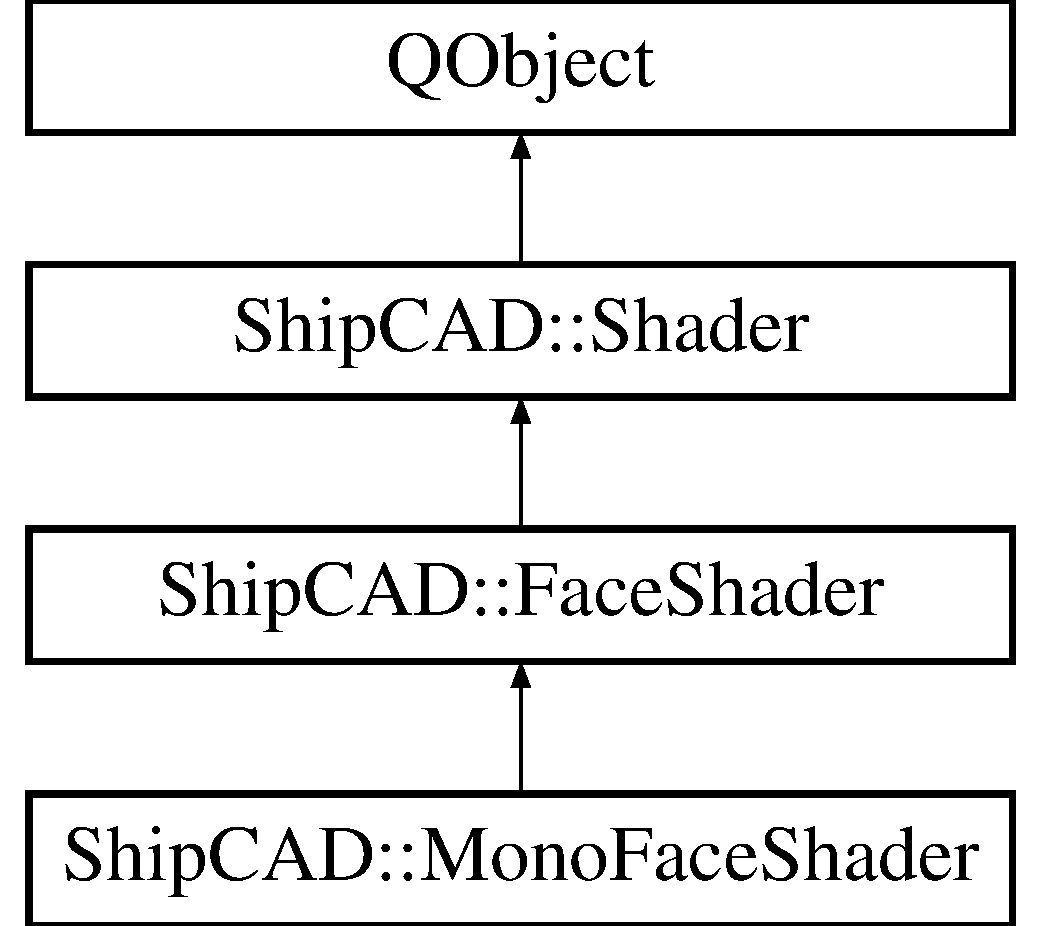
\includegraphics[height=3.000000cm]{classShipCAD_1_1MonoFaceShader}
\end{center}
\end{figure}
\subsection*{Public Member Functions}
\begin{DoxyCompactItemize}
\item 
\hyperlink{classShipCAD_1_1MonoFaceShader_a963aa389c930d6482a58f49b2ccb4473}{Mono\-Face\-Shader} (\hyperlink{classShipCAD_1_1Viewport}{Viewport} $\ast$vp)
\item 
virtual \hyperlink{classShipCAD_1_1MonoFaceShader_ab1f3cb853a5a2b04f9c4944d9eca30b4}{$\sim$\-Mono\-Face\-Shader} ()
\item 
virtual void \hyperlink{classShipCAD_1_1MonoFaceShader_a9a358ec63af4b067449e772cbc735d5a}{render\-Mesh} (Q\-Color mesh\-Color, Q\-Vector$<$ Q\-Vector3\-D $>$ \&vertices, Q\-Vector$<$ Q\-Vector3\-D $>$ \&normals)
\end{DoxyCompactItemize}
\subsection*{Additional Inherited Members}


\subsection{Detailed Description}


Definition at line 92 of file shader.\-h.



\subsection{Constructor \& Destructor Documentation}
\hypertarget{classShipCAD_1_1MonoFaceShader_a963aa389c930d6482a58f49b2ccb4473}{\index{Ship\-C\-A\-D\-::\-Mono\-Face\-Shader@{Ship\-C\-A\-D\-::\-Mono\-Face\-Shader}!Mono\-Face\-Shader@{Mono\-Face\-Shader}}
\index{Mono\-Face\-Shader@{Mono\-Face\-Shader}!ShipCAD::MonoFaceShader@{Ship\-C\-A\-D\-::\-Mono\-Face\-Shader}}
\subsubsection[{Mono\-Face\-Shader}]{\setlength{\rightskip}{0pt plus 5cm}Mono\-Face\-Shader\-::\-Mono\-Face\-Shader (
\begin{DoxyParamCaption}
\item[{{\bf Viewport} $\ast$}]{vp}
\end{DoxyParamCaption}
)\hspace{0.3cm}{\ttfamily [explicit]}}}\label{classShipCAD_1_1MonoFaceShader_a963aa389c930d6482a58f49b2ccb4473}


Definition at line 177 of file shader.\-cpp.

\hypertarget{classShipCAD_1_1MonoFaceShader_ab1f3cb853a5a2b04f9c4944d9eca30b4}{\index{Ship\-C\-A\-D\-::\-Mono\-Face\-Shader@{Ship\-C\-A\-D\-::\-Mono\-Face\-Shader}!$\sim$\-Mono\-Face\-Shader@{$\sim$\-Mono\-Face\-Shader}}
\index{$\sim$\-Mono\-Face\-Shader@{$\sim$\-Mono\-Face\-Shader}!ShipCAD::MonoFaceShader@{Ship\-C\-A\-D\-::\-Mono\-Face\-Shader}}
\subsubsection[{$\sim$\-Mono\-Face\-Shader}]{\setlength{\rightskip}{0pt plus 5cm}virtual Ship\-C\-A\-D\-::\-Mono\-Face\-Shader\-::$\sim$\-Mono\-Face\-Shader (
\begin{DoxyParamCaption}
{}
\end{DoxyParamCaption}
)\hspace{0.3cm}{\ttfamily [inline]}, {\ttfamily [virtual]}}}\label{classShipCAD_1_1MonoFaceShader_ab1f3cb853a5a2b04f9c4944d9eca30b4}


Definition at line 99 of file shader.\-h.



\subsection{Member Function Documentation}
\hypertarget{classShipCAD_1_1MonoFaceShader_a9a358ec63af4b067449e772cbc735d5a}{\index{Ship\-C\-A\-D\-::\-Mono\-Face\-Shader@{Ship\-C\-A\-D\-::\-Mono\-Face\-Shader}!render\-Mesh@{render\-Mesh}}
\index{render\-Mesh@{render\-Mesh}!ShipCAD::MonoFaceShader@{Ship\-C\-A\-D\-::\-Mono\-Face\-Shader}}
\subsubsection[{render\-Mesh}]{\setlength{\rightskip}{0pt plus 5cm}void Mono\-Face\-Shader\-::render\-Mesh (
\begin{DoxyParamCaption}
\item[{Q\-Color}]{mesh\-Color, }
\item[{Q\-Vector$<$ Q\-Vector3\-D $>$ \&}]{vertices, }
\item[{Q\-Vector$<$ Q\-Vector3\-D $>$ \&}]{normals}
\end{DoxyParamCaption}
)\hspace{0.3cm}{\ttfamily [virtual]}}}\label{classShipCAD_1_1MonoFaceShader_a9a358ec63af4b067449e772cbc735d5a}


Definition at line 188 of file shader.\-cpp.



The documentation for this class was generated from the following files\-:\begin{DoxyCompactItemize}
\item 
Ship\-C\-A\-Dlib/\hyperlink{shader_8h}{shader.\-h}\item 
Ship\-C\-A\-Dlib/\hyperlink{shader_8cpp}{shader.\-cpp}\end{DoxyCompactItemize}

\hypertarget{classShipCAD_1_1NURBSurface}{\section{Ship\-C\-A\-D\-:\-:N\-U\-R\-B\-Surface Class Reference}
\label{classShipCAD_1_1NURBSurface}\index{Ship\-C\-A\-D\-::\-N\-U\-R\-B\-Surface@{Ship\-C\-A\-D\-::\-N\-U\-R\-B\-Surface}}
}


{\ttfamily \#include $<$nurbsurface.\-h$>$}

Inheritance diagram for Ship\-C\-A\-D\-:\-:N\-U\-R\-B\-Surface\-:\begin{figure}[H]
\begin{center}
\leavevmode
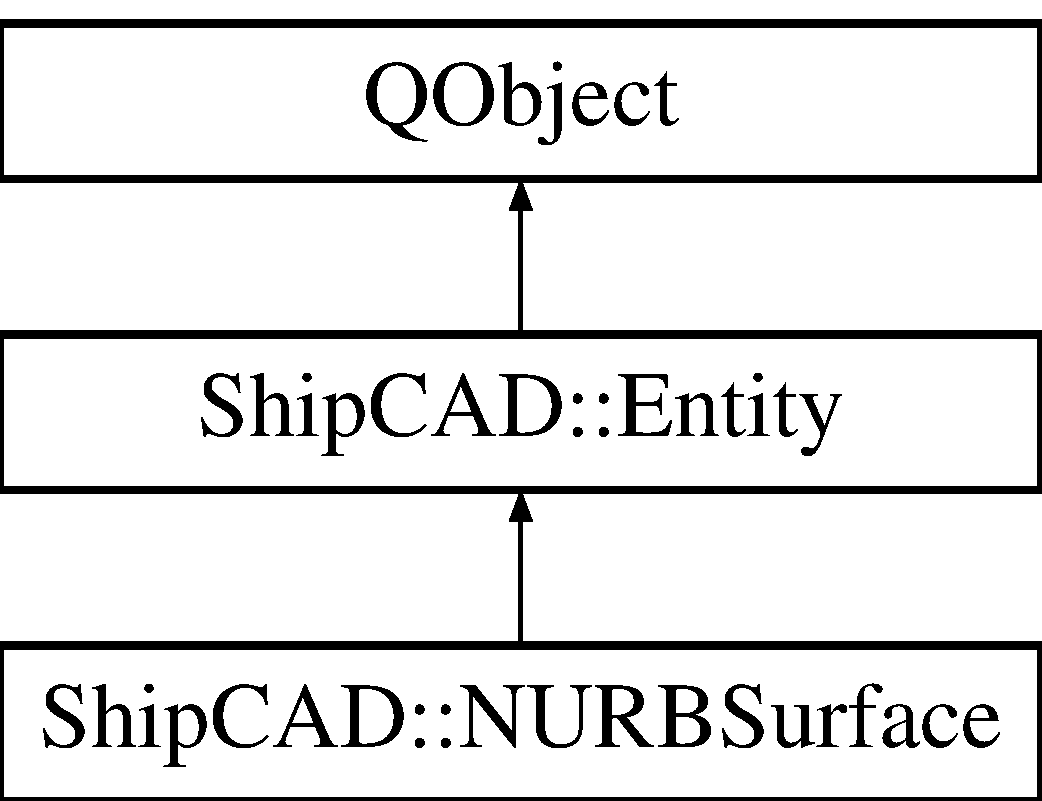
\includegraphics[height=3.000000cm]{classShipCAD_1_1NURBSurface}
\end{center}
\end{figure}
\subsection*{Public Member Functions}
\begin{DoxyCompactItemize}
\item 
\hyperlink{classShipCAD_1_1NURBSurface_ac01a08234a1d2a5e44d68a7393ef131c}{N\-U\-R\-B\-Surface} ()
\item 
virtual \hyperlink{classShipCAD_1_1NURBSurface_a333394fe5adc78a853d8784f4d2e87c6}{$\sim$\-N\-U\-R\-B\-Surface} ()
\item 
virtual void \hyperlink{classShipCAD_1_1NURBSurface_a5013b0c1e511ea68909eef5d0473d032}{clear} ()
\item 
virtual void \hyperlink{classShipCAD_1_1NURBSurface_a643231ea9a8f26e528a1d9a0dccf4070}{rebuild} ()
\item 
virtual void \hyperlink{classShipCAD_1_1NURBSurface_a9ee8f8aea431fe9f465080ec9f5624f9}{draw} (\hyperlink{classShipCAD_1_1Viewport}{Viewport} \&vp)
\item 
Q\-Vector3\-D \hyperlink{classShipCAD_1_1NURBSurface_a30435ae8689f09400b7754e4d7b3242a}{get\-Point} (size\-\_\-t row, size\-\_\-t col)
\item 
void \hyperlink{classShipCAD_1_1NURBSurface_a12217816f19b7de790ae9ed5cc784887}{set\-Col\-Degree} (size\-\_\-t val)
\item 
void \hyperlink{classShipCAD_1_1NURBSurface_a1f71f4cdf57f3f93aeaba0e7705d18f4}{set\-Row\-Degree} (size\-\_\-t val)
\item 
void \hyperlink{classShipCAD_1_1NURBSurface_aca43db0a1f829e101c4df124a4490031}{set\-Point} (size\-\_\-t row, size\-\_\-t col, const Q\-Vector3\-D \&val)
\item 
virtual void \hyperlink{classShipCAD_1_1NURBSurface_aa6fc3d060087593349ce1b5119419433}{set\-Build} (bool val)
\item 
void \hyperlink{classShipCAD_1_1NURBSurface_ad94a4350cda13ed3971ccf7bedaa1f10}{dump} (std\-::ostream \&os) const 
\end{DoxyCompactItemize}
\subsection*{Protected Attributes}
\begin{DoxyCompactItemize}
\item 
int \hyperlink{classShipCAD_1_1NURBSurface_aac0a2d528cec007b0fb6a154f3a67672}{\-\_\-col\-\_\-count}
\item 
int \hyperlink{classShipCAD_1_1NURBSurface_a251739da98a877b8d68722db5aa59371}{\-\_\-row\-\_\-count}
\item 
int \hyperlink{classShipCAD_1_1NURBSurface_a0192ed41981e4a3525f52be71ceb0e7c}{\-\_\-col\-\_\-degree}
\item 
int \hyperlink{classShipCAD_1_1NURBSurface_a0c53705ad7cc3004e60398f38909f59e}{\-\_\-row\-\_\-degree}
\item 
int \hyperlink{classShipCAD_1_1NURBSurface_a2b0e2649a54a57a9ae6fbeed031b04d0}{\-\_\-col\-\_\-knots}
\item 
int \hyperlink{classShipCAD_1_1NURBSurface_a3799680ea0e67d5d6c1a694f378e70ed}{\-\_\-row\-\_\-knots}
\item 
std\-::vector$<$ Q\-Vector3\-D $>$ \hyperlink{classShipCAD_1_1NURBSurface_a371421f0aec85ad3cffc3dbeeb0b26e4}{\-\_\-points}
\item 
std\-::vector$<$ bool $>$ \hyperlink{classShipCAD_1_1NURBSurface_a6f1765a2698b4ed79f0d110409129c28}{\-\_\-knuckles}
\item 
std\-::vector$<$ float $>$ \hyperlink{classShipCAD_1_1NURBSurface_a6de7536d23d408368f2df4470c1514af}{\-\_\-parameters}
\item 
std\-::vector$<$ Q\-Vector3\-D $>$ \hyperlink{classShipCAD_1_1NURBSurface_a6fa7cce7b1c78fc8fc89be24cba4d9b0}{\-\_\-derivatives}
\end{DoxyCompactItemize}
\subsection*{Additional Inherited Members}


\subsection{Detailed Description}


Definition at line 43 of file nurbsurface.\-h.



\subsection{Constructor \& Destructor Documentation}
\hypertarget{classShipCAD_1_1NURBSurface_ac01a08234a1d2a5e44d68a7393ef131c}{\index{Ship\-C\-A\-D\-::\-N\-U\-R\-B\-Surface@{Ship\-C\-A\-D\-::\-N\-U\-R\-B\-Surface}!N\-U\-R\-B\-Surface@{N\-U\-R\-B\-Surface}}
\index{N\-U\-R\-B\-Surface@{N\-U\-R\-B\-Surface}!ShipCAD::NURBSurface@{Ship\-C\-A\-D\-::\-N\-U\-R\-B\-Surface}}
\subsubsection[{N\-U\-R\-B\-Surface}]{\setlength{\rightskip}{0pt plus 5cm}N\-U\-R\-B\-Surface\-::\-N\-U\-R\-B\-Surface (
\begin{DoxyParamCaption}
{}
\end{DoxyParamCaption}
)\hspace{0.3cm}{\ttfamily [explicit]}}}\label{classShipCAD_1_1NURBSurface_ac01a08234a1d2a5e44d68a7393ef131c}


Definition at line 40 of file nurbsurface.\-cpp.

\hypertarget{classShipCAD_1_1NURBSurface_a333394fe5adc78a853d8784f4d2e87c6}{\index{Ship\-C\-A\-D\-::\-N\-U\-R\-B\-Surface@{Ship\-C\-A\-D\-::\-N\-U\-R\-B\-Surface}!$\sim$\-N\-U\-R\-B\-Surface@{$\sim$\-N\-U\-R\-B\-Surface}}
\index{$\sim$\-N\-U\-R\-B\-Surface@{$\sim$\-N\-U\-R\-B\-Surface}!ShipCAD::NURBSurface@{Ship\-C\-A\-D\-::\-N\-U\-R\-B\-Surface}}
\subsubsection[{$\sim$\-N\-U\-R\-B\-Surface}]{\setlength{\rightskip}{0pt plus 5cm}virtual Ship\-C\-A\-D\-::\-N\-U\-R\-B\-Surface\-::$\sim$\-N\-U\-R\-B\-Surface (
\begin{DoxyParamCaption}
{}
\end{DoxyParamCaption}
)\hspace{0.3cm}{\ttfamily [inline]}, {\ttfamily [virtual]}}}\label{classShipCAD_1_1NURBSurface_a333394fe5adc78a853d8784f4d2e87c6}


Definition at line 50 of file nurbsurface.\-h.



\subsection{Member Function Documentation}
\hypertarget{classShipCAD_1_1NURBSurface_a5013b0c1e511ea68909eef5d0473d032}{\index{Ship\-C\-A\-D\-::\-N\-U\-R\-B\-Surface@{Ship\-C\-A\-D\-::\-N\-U\-R\-B\-Surface}!clear@{clear}}
\index{clear@{clear}!ShipCAD::NURBSurface@{Ship\-C\-A\-D\-::\-N\-U\-R\-B\-Surface}}
\subsubsection[{clear}]{\setlength{\rightskip}{0pt plus 5cm}void N\-U\-R\-B\-Surface\-::clear (
\begin{DoxyParamCaption}
{}
\end{DoxyParamCaption}
)\hspace{0.3cm}{\ttfamily [virtual]}}}\label{classShipCAD_1_1NURBSurface_a5013b0c1e511ea68909eef5d0473d032}


Reimplemented from \hyperlink{classShipCAD_1_1Entity_a998d0e5d360371046fd5835ba1e0877a}{Ship\-C\-A\-D\-::\-Entity}.



Definition at line 72 of file nurbsurface.\-cpp.

\hypertarget{classShipCAD_1_1NURBSurface_a9ee8f8aea431fe9f465080ec9f5624f9}{\index{Ship\-C\-A\-D\-::\-N\-U\-R\-B\-Surface@{Ship\-C\-A\-D\-::\-N\-U\-R\-B\-Surface}!draw@{draw}}
\index{draw@{draw}!ShipCAD::NURBSurface@{Ship\-C\-A\-D\-::\-N\-U\-R\-B\-Surface}}
\subsubsection[{draw}]{\setlength{\rightskip}{0pt plus 5cm}void N\-U\-R\-B\-Surface\-::draw (
\begin{DoxyParamCaption}
\item[{{\bf Viewport} \&}]{vp}
\end{DoxyParamCaption}
)\hspace{0.3cm}{\ttfamily [virtual]}}}\label{classShipCAD_1_1NURBSurface_a9ee8f8aea431fe9f465080ec9f5624f9}


Definition at line 68 of file nurbsurface.\-cpp.

\hypertarget{classShipCAD_1_1NURBSurface_ad94a4350cda13ed3971ccf7bedaa1f10}{\index{Ship\-C\-A\-D\-::\-N\-U\-R\-B\-Surface@{Ship\-C\-A\-D\-::\-N\-U\-R\-B\-Surface}!dump@{dump}}
\index{dump@{dump}!ShipCAD::NURBSurface@{Ship\-C\-A\-D\-::\-N\-U\-R\-B\-Surface}}
\subsubsection[{dump}]{\setlength{\rightskip}{0pt plus 5cm}void N\-U\-R\-B\-Surface\-::dump (
\begin{DoxyParamCaption}
\item[{std\-::ostream \&}]{os}
\end{DoxyParamCaption}
) const}}\label{classShipCAD_1_1NURBSurface_ad94a4350cda13ed3971ccf7bedaa1f10}


Definition at line 76 of file nurbsurface.\-cpp.

\hypertarget{classShipCAD_1_1NURBSurface_a30435ae8689f09400b7754e4d7b3242a}{\index{Ship\-C\-A\-D\-::\-N\-U\-R\-B\-Surface@{Ship\-C\-A\-D\-::\-N\-U\-R\-B\-Surface}!get\-Point@{get\-Point}}
\index{get\-Point@{get\-Point}!ShipCAD::NURBSurface@{Ship\-C\-A\-D\-::\-N\-U\-R\-B\-Surface}}
\subsubsection[{get\-Point}]{\setlength{\rightskip}{0pt plus 5cm}Q\-Vector3\-D N\-U\-R\-B\-Surface\-::get\-Point (
\begin{DoxyParamCaption}
\item[{size\-\_\-t}]{row, }
\item[{size\-\_\-t}]{col}
\end{DoxyParamCaption}
)}}\label{classShipCAD_1_1NURBSurface_a30435ae8689f09400b7754e4d7b3242a}


Definition at line 57 of file nurbsurface.\-cpp.

\hypertarget{classShipCAD_1_1NURBSurface_a643231ea9a8f26e528a1d9a0dccf4070}{\index{Ship\-C\-A\-D\-::\-N\-U\-R\-B\-Surface@{Ship\-C\-A\-D\-::\-N\-U\-R\-B\-Surface}!rebuild@{rebuild}}
\index{rebuild@{rebuild}!ShipCAD::NURBSurface@{Ship\-C\-A\-D\-::\-N\-U\-R\-B\-Surface}}
\subsubsection[{rebuild}]{\setlength{\rightskip}{0pt plus 5cm}void N\-U\-R\-B\-Surface\-::rebuild (
\begin{DoxyParamCaption}
{}
\end{DoxyParamCaption}
)\hspace{0.3cm}{\ttfamily [virtual]}}}\label{classShipCAD_1_1NURBSurface_a643231ea9a8f26e528a1d9a0dccf4070}


Implements \hyperlink{classShipCAD_1_1Entity_a2571654319df6ad6841a437be7a75395}{Ship\-C\-A\-D\-::\-Entity}.



Definition at line 62 of file nurbsurface.\-cpp.

\hypertarget{classShipCAD_1_1NURBSurface_aa6fc3d060087593349ce1b5119419433}{\index{Ship\-C\-A\-D\-::\-N\-U\-R\-B\-Surface@{Ship\-C\-A\-D\-::\-N\-U\-R\-B\-Surface}!set\-Build@{set\-Build}}
\index{set\-Build@{set\-Build}!ShipCAD::NURBSurface@{Ship\-C\-A\-D\-::\-N\-U\-R\-B\-Surface}}
\subsubsection[{set\-Build}]{\setlength{\rightskip}{0pt plus 5cm}void N\-U\-R\-B\-Surface\-::set\-Build (
\begin{DoxyParamCaption}
\item[{bool}]{val}
\end{DoxyParamCaption}
)\hspace{0.3cm}{\ttfamily [virtual]}}}\label{classShipCAD_1_1NURBSurface_aa6fc3d060087593349ce1b5119419433}


Reimplemented from \hyperlink{classShipCAD_1_1Entity_a1889198398f42bb7f77a2334031c3f33}{Ship\-C\-A\-D\-::\-Entity}.



Definition at line 46 of file nurbsurface.\-cpp.

\hypertarget{classShipCAD_1_1NURBSurface_a12217816f19b7de790ae9ed5cc784887}{\index{Ship\-C\-A\-D\-::\-N\-U\-R\-B\-Surface@{Ship\-C\-A\-D\-::\-N\-U\-R\-B\-Surface}!set\-Col\-Degree@{set\-Col\-Degree}}
\index{set\-Col\-Degree@{set\-Col\-Degree}!ShipCAD::NURBSurface@{Ship\-C\-A\-D\-::\-N\-U\-R\-B\-Surface}}
\subsubsection[{set\-Col\-Degree}]{\setlength{\rightskip}{0pt plus 5cm}void Ship\-C\-A\-D\-::\-N\-U\-R\-B\-Surface\-::set\-Col\-Degree (
\begin{DoxyParamCaption}
\item[{size\-\_\-t}]{val}
\end{DoxyParamCaption}
)}}\label{classShipCAD_1_1NURBSurface_a12217816f19b7de790ae9ed5cc784887}
\hypertarget{classShipCAD_1_1NURBSurface_aca43db0a1f829e101c4df124a4490031}{\index{Ship\-C\-A\-D\-::\-N\-U\-R\-B\-Surface@{Ship\-C\-A\-D\-::\-N\-U\-R\-B\-Surface}!set\-Point@{set\-Point}}
\index{set\-Point@{set\-Point}!ShipCAD::NURBSurface@{Ship\-C\-A\-D\-::\-N\-U\-R\-B\-Surface}}
\subsubsection[{set\-Point}]{\setlength{\rightskip}{0pt plus 5cm}void N\-U\-R\-B\-Surface\-::set\-Point (
\begin{DoxyParamCaption}
\item[{size\-\_\-t}]{row, }
\item[{size\-\_\-t}]{col, }
\item[{const Q\-Vector3\-D \&}]{val}
\end{DoxyParamCaption}
)}}\label{classShipCAD_1_1NURBSurface_aca43db0a1f829e101c4df124a4490031}


Definition at line 53 of file nurbsurface.\-cpp.

\hypertarget{classShipCAD_1_1NURBSurface_a1f71f4cdf57f3f93aeaba0e7705d18f4}{\index{Ship\-C\-A\-D\-::\-N\-U\-R\-B\-Surface@{Ship\-C\-A\-D\-::\-N\-U\-R\-B\-Surface}!set\-Row\-Degree@{set\-Row\-Degree}}
\index{set\-Row\-Degree@{set\-Row\-Degree}!ShipCAD::NURBSurface@{Ship\-C\-A\-D\-::\-N\-U\-R\-B\-Surface}}
\subsubsection[{set\-Row\-Degree}]{\setlength{\rightskip}{0pt plus 5cm}void Ship\-C\-A\-D\-::\-N\-U\-R\-B\-Surface\-::set\-Row\-Degree (
\begin{DoxyParamCaption}
\item[{size\-\_\-t}]{val}
\end{DoxyParamCaption}
)}}\label{classShipCAD_1_1NURBSurface_a1f71f4cdf57f3f93aeaba0e7705d18f4}


\subsection{Member Data Documentation}
\hypertarget{classShipCAD_1_1NURBSurface_aac0a2d528cec007b0fb6a154f3a67672}{\index{Ship\-C\-A\-D\-::\-N\-U\-R\-B\-Surface@{Ship\-C\-A\-D\-::\-N\-U\-R\-B\-Surface}!\-\_\-col\-\_\-count@{\-\_\-col\-\_\-count}}
\index{\-\_\-col\-\_\-count@{\-\_\-col\-\_\-count}!ShipCAD::NURBSurface@{Ship\-C\-A\-D\-::\-N\-U\-R\-B\-Surface}}
\subsubsection[{\-\_\-col\-\_\-count}]{\setlength{\rightskip}{0pt plus 5cm}int Ship\-C\-A\-D\-::\-N\-U\-R\-B\-Surface\-::\-\_\-col\-\_\-count\hspace{0.3cm}{\ttfamily [protected]}}}\label{classShipCAD_1_1NURBSurface_aac0a2d528cec007b0fb6a154f3a67672}


Definition at line 78 of file nurbsurface.\-h.

\hypertarget{classShipCAD_1_1NURBSurface_a0192ed41981e4a3525f52be71ceb0e7c}{\index{Ship\-C\-A\-D\-::\-N\-U\-R\-B\-Surface@{Ship\-C\-A\-D\-::\-N\-U\-R\-B\-Surface}!\-\_\-col\-\_\-degree@{\-\_\-col\-\_\-degree}}
\index{\-\_\-col\-\_\-degree@{\-\_\-col\-\_\-degree}!ShipCAD::NURBSurface@{Ship\-C\-A\-D\-::\-N\-U\-R\-B\-Surface}}
\subsubsection[{\-\_\-col\-\_\-degree}]{\setlength{\rightskip}{0pt plus 5cm}int Ship\-C\-A\-D\-::\-N\-U\-R\-B\-Surface\-::\-\_\-col\-\_\-degree\hspace{0.3cm}{\ttfamily [protected]}}}\label{classShipCAD_1_1NURBSurface_a0192ed41981e4a3525f52be71ceb0e7c}


Definition at line 80 of file nurbsurface.\-h.

\hypertarget{classShipCAD_1_1NURBSurface_a2b0e2649a54a57a9ae6fbeed031b04d0}{\index{Ship\-C\-A\-D\-::\-N\-U\-R\-B\-Surface@{Ship\-C\-A\-D\-::\-N\-U\-R\-B\-Surface}!\-\_\-col\-\_\-knots@{\-\_\-col\-\_\-knots}}
\index{\-\_\-col\-\_\-knots@{\-\_\-col\-\_\-knots}!ShipCAD::NURBSurface@{Ship\-C\-A\-D\-::\-N\-U\-R\-B\-Surface}}
\subsubsection[{\-\_\-col\-\_\-knots}]{\setlength{\rightskip}{0pt plus 5cm}int Ship\-C\-A\-D\-::\-N\-U\-R\-B\-Surface\-::\-\_\-col\-\_\-knots\hspace{0.3cm}{\ttfamily [protected]}}}\label{classShipCAD_1_1NURBSurface_a2b0e2649a54a57a9ae6fbeed031b04d0}


Definition at line 82 of file nurbsurface.\-h.

\hypertarget{classShipCAD_1_1NURBSurface_a6fa7cce7b1c78fc8fc89be24cba4d9b0}{\index{Ship\-C\-A\-D\-::\-N\-U\-R\-B\-Surface@{Ship\-C\-A\-D\-::\-N\-U\-R\-B\-Surface}!\-\_\-derivatives@{\-\_\-derivatives}}
\index{\-\_\-derivatives@{\-\_\-derivatives}!ShipCAD::NURBSurface@{Ship\-C\-A\-D\-::\-N\-U\-R\-B\-Surface}}
\subsubsection[{\-\_\-derivatives}]{\setlength{\rightskip}{0pt plus 5cm}std\-::vector$<$Q\-Vector3\-D$>$ Ship\-C\-A\-D\-::\-N\-U\-R\-B\-Surface\-::\-\_\-derivatives\hspace{0.3cm}{\ttfamily [protected]}}}\label{classShipCAD_1_1NURBSurface_a6fa7cce7b1c78fc8fc89be24cba4d9b0}


Definition at line 88 of file nurbsurface.\-h.

\hypertarget{classShipCAD_1_1NURBSurface_a6f1765a2698b4ed79f0d110409129c28}{\index{Ship\-C\-A\-D\-::\-N\-U\-R\-B\-Surface@{Ship\-C\-A\-D\-::\-N\-U\-R\-B\-Surface}!\-\_\-knuckles@{\-\_\-knuckles}}
\index{\-\_\-knuckles@{\-\_\-knuckles}!ShipCAD::NURBSurface@{Ship\-C\-A\-D\-::\-N\-U\-R\-B\-Surface}}
\subsubsection[{\-\_\-knuckles}]{\setlength{\rightskip}{0pt plus 5cm}std\-::vector$<$bool$>$ Ship\-C\-A\-D\-::\-N\-U\-R\-B\-Surface\-::\-\_\-knuckles\hspace{0.3cm}{\ttfamily [protected]}}}\label{classShipCAD_1_1NURBSurface_a6f1765a2698b4ed79f0d110409129c28}


Definition at line 86 of file nurbsurface.\-h.

\hypertarget{classShipCAD_1_1NURBSurface_a6de7536d23d408368f2df4470c1514af}{\index{Ship\-C\-A\-D\-::\-N\-U\-R\-B\-Surface@{Ship\-C\-A\-D\-::\-N\-U\-R\-B\-Surface}!\-\_\-parameters@{\-\_\-parameters}}
\index{\-\_\-parameters@{\-\_\-parameters}!ShipCAD::NURBSurface@{Ship\-C\-A\-D\-::\-N\-U\-R\-B\-Surface}}
\subsubsection[{\-\_\-parameters}]{\setlength{\rightskip}{0pt plus 5cm}std\-::vector$<$float$>$ Ship\-C\-A\-D\-::\-N\-U\-R\-B\-Surface\-::\-\_\-parameters\hspace{0.3cm}{\ttfamily [protected]}}}\label{classShipCAD_1_1NURBSurface_a6de7536d23d408368f2df4470c1514af}


Definition at line 87 of file nurbsurface.\-h.

\hypertarget{classShipCAD_1_1NURBSurface_a371421f0aec85ad3cffc3dbeeb0b26e4}{\index{Ship\-C\-A\-D\-::\-N\-U\-R\-B\-Surface@{Ship\-C\-A\-D\-::\-N\-U\-R\-B\-Surface}!\-\_\-points@{\-\_\-points}}
\index{\-\_\-points@{\-\_\-points}!ShipCAD::NURBSurface@{Ship\-C\-A\-D\-::\-N\-U\-R\-B\-Surface}}
\subsubsection[{\-\_\-points}]{\setlength{\rightskip}{0pt plus 5cm}std\-::vector$<$Q\-Vector3\-D$>$ Ship\-C\-A\-D\-::\-N\-U\-R\-B\-Surface\-::\-\_\-points\hspace{0.3cm}{\ttfamily [protected]}}}\label{classShipCAD_1_1NURBSurface_a371421f0aec85ad3cffc3dbeeb0b26e4}


Definition at line 85 of file nurbsurface.\-h.

\hypertarget{classShipCAD_1_1NURBSurface_a251739da98a877b8d68722db5aa59371}{\index{Ship\-C\-A\-D\-::\-N\-U\-R\-B\-Surface@{Ship\-C\-A\-D\-::\-N\-U\-R\-B\-Surface}!\-\_\-row\-\_\-count@{\-\_\-row\-\_\-count}}
\index{\-\_\-row\-\_\-count@{\-\_\-row\-\_\-count}!ShipCAD::NURBSurface@{Ship\-C\-A\-D\-::\-N\-U\-R\-B\-Surface}}
\subsubsection[{\-\_\-row\-\_\-count}]{\setlength{\rightskip}{0pt plus 5cm}int Ship\-C\-A\-D\-::\-N\-U\-R\-B\-Surface\-::\-\_\-row\-\_\-count\hspace{0.3cm}{\ttfamily [protected]}}}\label{classShipCAD_1_1NURBSurface_a251739da98a877b8d68722db5aa59371}


Definition at line 79 of file nurbsurface.\-h.

\hypertarget{classShipCAD_1_1NURBSurface_a0c53705ad7cc3004e60398f38909f59e}{\index{Ship\-C\-A\-D\-::\-N\-U\-R\-B\-Surface@{Ship\-C\-A\-D\-::\-N\-U\-R\-B\-Surface}!\-\_\-row\-\_\-degree@{\-\_\-row\-\_\-degree}}
\index{\-\_\-row\-\_\-degree@{\-\_\-row\-\_\-degree}!ShipCAD::NURBSurface@{Ship\-C\-A\-D\-::\-N\-U\-R\-B\-Surface}}
\subsubsection[{\-\_\-row\-\_\-degree}]{\setlength{\rightskip}{0pt plus 5cm}int Ship\-C\-A\-D\-::\-N\-U\-R\-B\-Surface\-::\-\_\-row\-\_\-degree\hspace{0.3cm}{\ttfamily [protected]}}}\label{classShipCAD_1_1NURBSurface_a0c53705ad7cc3004e60398f38909f59e}


Definition at line 81 of file nurbsurface.\-h.

\hypertarget{classShipCAD_1_1NURBSurface_a3799680ea0e67d5d6c1a694f378e70ed}{\index{Ship\-C\-A\-D\-::\-N\-U\-R\-B\-Surface@{Ship\-C\-A\-D\-::\-N\-U\-R\-B\-Surface}!\-\_\-row\-\_\-knots@{\-\_\-row\-\_\-knots}}
\index{\-\_\-row\-\_\-knots@{\-\_\-row\-\_\-knots}!ShipCAD::NURBSurface@{Ship\-C\-A\-D\-::\-N\-U\-R\-B\-Surface}}
\subsubsection[{\-\_\-row\-\_\-knots}]{\setlength{\rightskip}{0pt plus 5cm}int Ship\-C\-A\-D\-::\-N\-U\-R\-B\-Surface\-::\-\_\-row\-\_\-knots\hspace{0.3cm}{\ttfamily [protected]}}}\label{classShipCAD_1_1NURBSurface_a3799680ea0e67d5d6c1a694f378e70ed}


Definition at line 83 of file nurbsurface.\-h.



The documentation for this class was generated from the following files\-:\begin{DoxyCompactItemize}
\item 
Ship\-C\-A\-Dlib/\hyperlink{nurbsurface_8h}{nurbsurface.\-h}\item 
Ship\-C\-A\-Dlib/\hyperlink{nurbsurface_8cpp}{nurbsurface.\-cpp}\end{DoxyCompactItemize}

\hypertarget{classOpenGLWindow}{\section{Open\-G\-L\-Window Class Reference}
\label{classOpenGLWindow}\index{Open\-G\-L\-Window@{Open\-G\-L\-Window}}
}


{\ttfamily \#include $<$openglwindow.\-h$>$}

Inheritance diagram for Open\-G\-L\-Window\-:\begin{figure}[H]
\begin{center}
\leavevmode
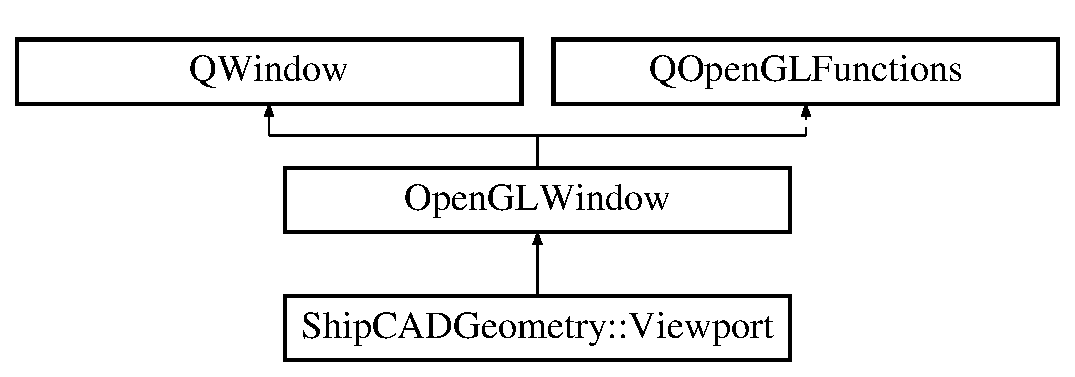
\includegraphics[height=3.000000cm]{classOpenGLWindow}
\end{center}
\end{figure}
\subsection*{Public Slots}
\begin{DoxyCompactItemize}
\item 
void \hyperlink{classOpenGLWindow_abea9e50147496e5110b86f03122fbece}{render\-Later} ()
\item 
void \hyperlink{classOpenGLWindow_a8398ed62d646739fe54fae94c477ad1d}{render\-Now} ()
\end{DoxyCompactItemize}
\subsection*{Public Member Functions}
\begin{DoxyCompactItemize}
\item 
\hyperlink{classOpenGLWindow_a90bb7dbb2dcb27b1fdc56ef4ef3f25fc}{Open\-G\-L\-Window} (Q\-Window $\ast$parent=0)
\item 
\hyperlink{classOpenGLWindow_aa220b192c71871aab9100f4058a8d62d}{$\sim$\-Open\-G\-L\-Window} ()
\item 
virtual void \hyperlink{classOpenGLWindow_a186cffcb57053e4eda4875b1ab9aac92}{render} (Q\-Painter $\ast$painter)
\item 
virtual void \hyperlink{classOpenGLWindow_ac9e094864803a0b29364f42c2a47fa8c}{render} ()
\item 
virtual void \hyperlink{classOpenGLWindow_aed4e2ee22e113b2f7e7d1eba4ef1b965}{initialize} ()
\item 
void \hyperlink{classOpenGLWindow_a68317e3284d7b0ffba262eac059b6b9e}{set\-Animating} (bool animating)
\end{DoxyCompactItemize}
\subsection*{Protected Member Functions}
\begin{DoxyCompactItemize}
\item 
bool \hyperlink{classOpenGLWindow_a1e3045cffb900de55b7384f5091c9d94}{event} (Q\-Event $\ast$event)
\item 
void \hyperlink{classOpenGLWindow_a991121ba7a4bbfa208fa74e5c86004c3}{expose\-Event} (Q\-Expose\-Event $\ast$\hyperlink{classOpenGLWindow_a1e3045cffb900de55b7384f5091c9d94}{event})
\item 
void \hyperlink{classOpenGLWindow_ae0e1d4dc039ce114ac615ce1dee38e51}{resize\-Event} (Q\-Resize\-Event $\ast$\hyperlink{classOpenGLWindow_a1e3045cffb900de55b7384f5091c9d94}{event})
\end{DoxyCompactItemize}


\subsection{Detailed Description}


Definition at line 75 of file openglwindow.\-h.



\subsection{Constructor \& Destructor Documentation}
\hypertarget{classOpenGLWindow_a90bb7dbb2dcb27b1fdc56ef4ef3f25fc}{\index{Open\-G\-L\-Window@{Open\-G\-L\-Window}!Open\-G\-L\-Window@{Open\-G\-L\-Window}}
\index{Open\-G\-L\-Window@{Open\-G\-L\-Window}!OpenGLWindow@{Open\-G\-L\-Window}}
\subsubsection[{Open\-G\-L\-Window}]{\setlength{\rightskip}{0pt plus 5cm}Open\-G\-L\-Window\-::\-Open\-G\-L\-Window (
\begin{DoxyParamCaption}
\item[{Q\-Window $\ast$}]{parent = {\ttfamily 0}}
\end{DoxyParamCaption}
)\hspace{0.3cm}{\ttfamily [explicit]}}}\label{classOpenGLWindow_a90bb7dbb2dcb27b1fdc56ef4ef3f25fc}


Definition at line 76 of file openglwindow.\-cpp.

\hypertarget{classOpenGLWindow_aa220b192c71871aab9100f4058a8d62d}{\index{Open\-G\-L\-Window@{Open\-G\-L\-Window}!$\sim$\-Open\-G\-L\-Window@{$\sim$\-Open\-G\-L\-Window}}
\index{$\sim$\-Open\-G\-L\-Window@{$\sim$\-Open\-G\-L\-Window}!OpenGLWindow@{Open\-G\-L\-Window}}
\subsubsection[{$\sim$\-Open\-G\-L\-Window}]{\setlength{\rightskip}{0pt plus 5cm}Open\-G\-L\-Window\-::$\sim$\-Open\-G\-L\-Window (
\begin{DoxyParamCaption}
{}
\end{DoxyParamCaption}
)}}\label{classOpenGLWindow_aa220b192c71871aab9100f4058a8d62d}


Definition at line 86 of file openglwindow.\-cpp.



\subsection{Member Function Documentation}
\hypertarget{classOpenGLWindow_a1e3045cffb900de55b7384f5091c9d94}{\index{Open\-G\-L\-Window@{Open\-G\-L\-Window}!event@{event}}
\index{event@{event}!OpenGLWindow@{Open\-G\-L\-Window}}
\subsubsection[{event}]{\setlength{\rightskip}{0pt plus 5cm}bool Open\-G\-L\-Window\-::event (
\begin{DoxyParamCaption}
\item[{Q\-Event $\ast$}]{event}
\end{DoxyParamCaption}
)\hspace{0.3cm}{\ttfamily [protected]}}}\label{classOpenGLWindow_a1e3045cffb900de55b7384f5091c9d94}


Definition at line 120 of file openglwindow.\-cpp.

\hypertarget{classOpenGLWindow_a991121ba7a4bbfa208fa74e5c86004c3}{\index{Open\-G\-L\-Window@{Open\-G\-L\-Window}!expose\-Event@{expose\-Event}}
\index{expose\-Event@{expose\-Event}!OpenGLWindow@{Open\-G\-L\-Window}}
\subsubsection[{expose\-Event}]{\setlength{\rightskip}{0pt plus 5cm}void Open\-G\-L\-Window\-::expose\-Event (
\begin{DoxyParamCaption}
\item[{Q\-Expose\-Event $\ast$}]{event}
\end{DoxyParamCaption}
)\hspace{0.3cm}{\ttfamily [protected]}}}\label{classOpenGLWindow_a991121ba7a4bbfa208fa74e5c86004c3}


Definition at line 131 of file openglwindow.\-cpp.

\hypertarget{classOpenGLWindow_aed4e2ee22e113b2f7e7d1eba4ef1b965}{\index{Open\-G\-L\-Window@{Open\-G\-L\-Window}!initialize@{initialize}}
\index{initialize@{initialize}!OpenGLWindow@{Open\-G\-L\-Window}}
\subsubsection[{initialize}]{\setlength{\rightskip}{0pt plus 5cm}void Open\-G\-L\-Window\-::initialize (
\begin{DoxyParamCaption}
{}
\end{DoxyParamCaption}
)\hspace{0.3cm}{\ttfamily [virtual]}}}\label{classOpenGLWindow_aed4e2ee22e113b2f7e7d1eba4ef1b965}


Reimplemented in \hyperlink{classShipCAD_1_1Viewport_a9c35de3f7c9d7c860c494081b48309b3}{Ship\-C\-A\-D\-::\-Viewport}.



Definition at line 95 of file openglwindow.\-cpp.

\hypertarget{classOpenGLWindow_a186cffcb57053e4eda4875b1ab9aac92}{\index{Open\-G\-L\-Window@{Open\-G\-L\-Window}!render@{render}}
\index{render@{render}!OpenGLWindow@{Open\-G\-L\-Window}}
\subsubsection[{render}]{\setlength{\rightskip}{0pt plus 5cm}void Open\-G\-L\-Window\-::render (
\begin{DoxyParamCaption}
\item[{Q\-Painter $\ast$}]{painter}
\end{DoxyParamCaption}
)\hspace{0.3cm}{\ttfamily [virtual]}}}\label{classOpenGLWindow_a186cffcb57053e4eda4875b1ab9aac92}


Definition at line 90 of file openglwindow.\-cpp.

\hypertarget{classOpenGLWindow_ac9e094864803a0b29364f42c2a47fa8c}{\index{Open\-G\-L\-Window@{Open\-G\-L\-Window}!render@{render}}
\index{render@{render}!OpenGLWindow@{Open\-G\-L\-Window}}
\subsubsection[{render}]{\setlength{\rightskip}{0pt plus 5cm}void Open\-G\-L\-Window\-::render (
\begin{DoxyParamCaption}
{}
\end{DoxyParamCaption}
)\hspace{0.3cm}{\ttfamily [virtual]}}}\label{classOpenGLWindow_ac9e094864803a0b29364f42c2a47fa8c}


Reimplemented in \hyperlink{classShipCAD_1_1Viewport_a9e81b526db3c2b508322c29b9fda5845}{Ship\-C\-A\-D\-::\-Viewport}.



Definition at line 99 of file openglwindow.\-cpp.

\hypertarget{classOpenGLWindow_abea9e50147496e5110b86f03122fbece}{\index{Open\-G\-L\-Window@{Open\-G\-L\-Window}!render\-Later@{render\-Later}}
\index{render\-Later@{render\-Later}!OpenGLWindow@{Open\-G\-L\-Window}}
\subsubsection[{render\-Later}]{\setlength{\rightskip}{0pt plus 5cm}void Open\-G\-L\-Window\-::render\-Later (
\begin{DoxyParamCaption}
{}
\end{DoxyParamCaption}
)\hspace{0.3cm}{\ttfamily [slot]}}}\label{classOpenGLWindow_abea9e50147496e5110b86f03122fbece}


Definition at line 112 of file openglwindow.\-cpp.

\hypertarget{classOpenGLWindow_a8398ed62d646739fe54fae94c477ad1d}{\index{Open\-G\-L\-Window@{Open\-G\-L\-Window}!render\-Now@{render\-Now}}
\index{render\-Now@{render\-Now}!OpenGLWindow@{Open\-G\-L\-Window}}
\subsubsection[{render\-Now}]{\setlength{\rightskip}{0pt plus 5cm}void Open\-G\-L\-Window\-::render\-Now (
\begin{DoxyParamCaption}
{}
\end{DoxyParamCaption}
)\hspace{0.3cm}{\ttfamily [slot]}}}\label{classOpenGLWindow_a8398ed62d646739fe54fae94c477ad1d}


Definition at line 147 of file openglwindow.\-cpp.

\hypertarget{classOpenGLWindow_ae0e1d4dc039ce114ac615ce1dee38e51}{\index{Open\-G\-L\-Window@{Open\-G\-L\-Window}!resize\-Event@{resize\-Event}}
\index{resize\-Event@{resize\-Event}!OpenGLWindow@{Open\-G\-L\-Window}}
\subsubsection[{resize\-Event}]{\setlength{\rightskip}{0pt plus 5cm}void Open\-G\-L\-Window\-::resize\-Event (
\begin{DoxyParamCaption}
\item[{Q\-Resize\-Event $\ast$}]{event}
\end{DoxyParamCaption}
)\hspace{0.3cm}{\ttfamily [protected]}}}\label{classOpenGLWindow_ae0e1d4dc039ce114ac615ce1dee38e51}


Definition at line 139 of file openglwindow.\-cpp.

\hypertarget{classOpenGLWindow_a68317e3284d7b0ffba262eac059b6b9e}{\index{Open\-G\-L\-Window@{Open\-G\-L\-Window}!set\-Animating@{set\-Animating}}
\index{set\-Animating@{set\-Animating}!OpenGLWindow@{Open\-G\-L\-Window}}
\subsubsection[{set\-Animating}]{\setlength{\rightskip}{0pt plus 5cm}void Open\-G\-L\-Window\-::set\-Animating (
\begin{DoxyParamCaption}
\item[{bool}]{animating}
\end{DoxyParamCaption}
)}}\label{classOpenGLWindow_a68317e3284d7b0ffba262eac059b6b9e}


Definition at line 179 of file openglwindow.\-cpp.



The documentation for this class was generated from the following files\-:\begin{DoxyCompactItemize}
\item 
Ship\-C\-A\-Dlib/\hyperlink{openglwindow_8h}{openglwindow.\-h}\item 
Ship\-C\-A\-Dlib/\hyperlink{openglwindow_8cpp}{openglwindow.\-cpp}\end{DoxyCompactItemize}

\hypertarget{classShipCAD_1_1Plane}{\section{Ship\-C\-A\-D\-:\-:Plane Class Reference}
\label{classShipCAD_1_1Plane}\index{Ship\-C\-A\-D\-::\-Plane@{Ship\-C\-A\-D\-::\-Plane}}
}


{\ttfamily \#include $<$plane.\-h$>$}

\subsection*{Public Member Functions}
\begin{DoxyCompactItemize}
\item 
\hyperlink{classShipCAD_1_1Plane_acac0d9c003e0ab10d07b146c3566a0c7}{Plane} ()
\item 
\hyperlink{classShipCAD_1_1Plane_a9a1420228e8baa632c7e8ba66f27772f}{Plane} (float \hyperlink{classShipCAD_1_1Plane_a1105f3715d9593c0971e0b0959859a84}{a}, float \hyperlink{classShipCAD_1_1Plane_adf79c9ba86dd3112fc098141195fcac5}{b}, float \hyperlink{classShipCAD_1_1Plane_a01b0067ca1a669aef5a8ab85bfce41cc}{c}, float \hyperlink{classShipCAD_1_1Plane_a7755d7967aae2e083c5d08fed49d9eef}{d})
\item 
\hyperlink{classShipCAD_1_1Plane_a254ddea0d760646007a19512e502e6fc}{Plane} (const Q\-Vector3\-D \&p, const Q\-Vector3\-D \&normal)
\item 
\hyperlink{classShipCAD_1_1Plane_adbaa1f5c7100e5592312359cb8eede37}{Plane} (const Q\-Vector3\-D \&p1, const Q\-Vector3\-D \&p2, const Q\-Vector3\-D \&p3)
\item 
\hyperlink{classShipCAD_1_1Plane_aff2204f8b2b25c201d172d4ec2518c77}{$\sim$\-Plane} ()
\item 
float \hyperlink{classShipCAD_1_1Plane_a1105f3715d9593c0971e0b0959859a84}{a} () const 
\item 
float \hyperlink{classShipCAD_1_1Plane_adf79c9ba86dd3112fc098141195fcac5}{b} () const 
\item 
float \hyperlink{classShipCAD_1_1Plane_a01b0067ca1a669aef5a8ab85bfce41cc}{c} () const 
\item 
float \hyperlink{classShipCAD_1_1Plane_a7755d7967aae2e083c5d08fed49d9eef}{d} () const 
\item 
void \hyperlink{classShipCAD_1_1Plane_a383a2f49031b8bcfa04be06035836a05}{set\-A} (float val)
\item 
void \hyperlink{classShipCAD_1_1Plane_aab7d46cba75a32089644b183e0a82dff}{set\-B} (float val)
\item 
void \hyperlink{classShipCAD_1_1Plane_affed6efd889f4725ae764b243763fb3e}{set\-C} (float val)
\item 
void \hyperlink{classShipCAD_1_1Plane_a5c3e18bcb1bb77563fd994866ba823df}{set\-D} (float val)
\item 
float \hyperlink{classShipCAD_1_1Plane_a6851b997a300848fcb37b33407165c44}{distance} (const Q\-Vector3\-D \&point) const 
\item 
bool \hyperlink{classShipCAD_1_1Plane_a76d5f22d213962e8ab0880fae3e919df}{intersects\-Box} (const Q\-Vector3\-D \&p1, const Q\-Vector3\-D \&p2) const 
\item 
Q\-Vector3\-D \hyperlink{classShipCAD_1_1Plane_af92620c1adaa989aa79cdcc13ce380da}{project\-Point\-On\-Plane} (const Q\-Vector3\-D \&p)
\begin{DoxyCompactList}\small\item\em project a point onto a plane \end{DoxyCompactList}\item 
bool \hyperlink{classShipCAD_1_1Plane_a8e9d8144407bbad413e14984a5fbed09}{intersect\-Line} (const Q\-Vector3\-D \&pt, const Q\-Vector3\-D \&n, bool \&coplanar, Q\-Vector3\-D \&intpt)
\begin{DoxyCompactList}\small\item\em intersect a line with this plane \end{DoxyCompactList}\end{DoxyCompactItemize}


\subsection{Detailed Description}


Definition at line 39 of file plane.\-h.



\subsection{Constructor \& Destructor Documentation}
\hypertarget{classShipCAD_1_1Plane_acac0d9c003e0ab10d07b146c3566a0c7}{\index{Ship\-C\-A\-D\-::\-Plane@{Ship\-C\-A\-D\-::\-Plane}!Plane@{Plane}}
\index{Plane@{Plane}!ShipCAD::Plane@{Ship\-C\-A\-D\-::\-Plane}}
\subsubsection[{Plane}]{\setlength{\rightskip}{0pt plus 5cm}Plane\-::\-Plane (
\begin{DoxyParamCaption}
{}
\end{DoxyParamCaption}
)\hspace{0.3cm}{\ttfamily [explicit]}}}\label{classShipCAD_1_1Plane_acac0d9c003e0ab10d07b146c3566a0c7}


Definition at line 37 of file plane.\-cpp.

\hypertarget{classShipCAD_1_1Plane_a9a1420228e8baa632c7e8ba66f27772f}{\index{Ship\-C\-A\-D\-::\-Plane@{Ship\-C\-A\-D\-::\-Plane}!Plane@{Plane}}
\index{Plane@{Plane}!ShipCAD::Plane@{Ship\-C\-A\-D\-::\-Plane}}
\subsubsection[{Plane}]{\setlength{\rightskip}{0pt plus 5cm}Plane\-::\-Plane (
\begin{DoxyParamCaption}
\item[{float}]{a, }
\item[{float}]{b, }
\item[{float}]{c, }
\item[{float}]{d}
\end{DoxyParamCaption}
)\hspace{0.3cm}{\ttfamily [explicit]}}}\label{classShipCAD_1_1Plane_a9a1420228e8baa632c7e8ba66f27772f}


Definition at line 42 of file plane.\-cpp.

\hypertarget{classShipCAD_1_1Plane_a254ddea0d760646007a19512e502e6fc}{\index{Ship\-C\-A\-D\-::\-Plane@{Ship\-C\-A\-D\-::\-Plane}!Plane@{Plane}}
\index{Plane@{Plane}!ShipCAD::Plane@{Ship\-C\-A\-D\-::\-Plane}}
\subsubsection[{Plane}]{\setlength{\rightskip}{0pt plus 5cm}Plane\-::\-Plane (
\begin{DoxyParamCaption}
\item[{const Q\-Vector3\-D \&}]{p, }
\item[{const Q\-Vector3\-D \&}]{normal}
\end{DoxyParamCaption}
)\hspace{0.3cm}{\ttfamily [explicit]}}}\label{classShipCAD_1_1Plane_a254ddea0d760646007a19512e502e6fc}


Definition at line 50 of file plane.\-cpp.

\hypertarget{classShipCAD_1_1Plane_adbaa1f5c7100e5592312359cb8eede37}{\index{Ship\-C\-A\-D\-::\-Plane@{Ship\-C\-A\-D\-::\-Plane}!Plane@{Plane}}
\index{Plane@{Plane}!ShipCAD::Plane@{Ship\-C\-A\-D\-::\-Plane}}
\subsubsection[{Plane}]{\setlength{\rightskip}{0pt plus 5cm}Plane\-::\-Plane (
\begin{DoxyParamCaption}
\item[{const Q\-Vector3\-D \&}]{p1, }
\item[{const Q\-Vector3\-D \&}]{p2, }
\item[{const Q\-Vector3\-D \&}]{p3}
\end{DoxyParamCaption}
)\hspace{0.3cm}{\ttfamily [explicit]}}}\label{classShipCAD_1_1Plane_adbaa1f5c7100e5592312359cb8eede37}


Definition at line 58 of file plane.\-cpp.

\hypertarget{classShipCAD_1_1Plane_aff2204f8b2b25c201d172d4ec2518c77}{\index{Ship\-C\-A\-D\-::\-Plane@{Ship\-C\-A\-D\-::\-Plane}!$\sim$\-Plane@{$\sim$\-Plane}}
\index{$\sim$\-Plane@{$\sim$\-Plane}!ShipCAD::Plane@{Ship\-C\-A\-D\-::\-Plane}}
\subsubsection[{$\sim$\-Plane}]{\setlength{\rightskip}{0pt plus 5cm}Ship\-C\-A\-D\-::\-Plane\-::$\sim$\-Plane (
\begin{DoxyParamCaption}
{}
\end{DoxyParamCaption}
)\hspace{0.3cm}{\ttfamily [inline]}}}\label{classShipCAD_1_1Plane_aff2204f8b2b25c201d172d4ec2518c77}


Definition at line 48 of file plane.\-h.



\subsection{Member Function Documentation}
\hypertarget{classShipCAD_1_1Plane_a1105f3715d9593c0971e0b0959859a84}{\index{Ship\-C\-A\-D\-::\-Plane@{Ship\-C\-A\-D\-::\-Plane}!a@{a}}
\index{a@{a}!ShipCAD::Plane@{Ship\-C\-A\-D\-::\-Plane}}
\subsubsection[{a}]{\setlength{\rightskip}{0pt plus 5cm}float Ship\-C\-A\-D\-::\-Plane\-::a (
\begin{DoxyParamCaption}
{}
\end{DoxyParamCaption}
) const\hspace{0.3cm}{\ttfamily [inline]}}}\label{classShipCAD_1_1Plane_a1105f3715d9593c0971e0b0959859a84}


Definition at line 50 of file plane.\-h.

\hypertarget{classShipCAD_1_1Plane_adf79c9ba86dd3112fc098141195fcac5}{\index{Ship\-C\-A\-D\-::\-Plane@{Ship\-C\-A\-D\-::\-Plane}!b@{b}}
\index{b@{b}!ShipCAD::Plane@{Ship\-C\-A\-D\-::\-Plane}}
\subsubsection[{b}]{\setlength{\rightskip}{0pt plus 5cm}float Ship\-C\-A\-D\-::\-Plane\-::b (
\begin{DoxyParamCaption}
{}
\end{DoxyParamCaption}
) const\hspace{0.3cm}{\ttfamily [inline]}}}\label{classShipCAD_1_1Plane_adf79c9ba86dd3112fc098141195fcac5}


Definition at line 52 of file plane.\-h.

\hypertarget{classShipCAD_1_1Plane_a01b0067ca1a669aef5a8ab85bfce41cc}{\index{Ship\-C\-A\-D\-::\-Plane@{Ship\-C\-A\-D\-::\-Plane}!c@{c}}
\index{c@{c}!ShipCAD::Plane@{Ship\-C\-A\-D\-::\-Plane}}
\subsubsection[{c}]{\setlength{\rightskip}{0pt plus 5cm}float Ship\-C\-A\-D\-::\-Plane\-::c (
\begin{DoxyParamCaption}
{}
\end{DoxyParamCaption}
) const\hspace{0.3cm}{\ttfamily [inline]}}}\label{classShipCAD_1_1Plane_a01b0067ca1a669aef5a8ab85bfce41cc}


Definition at line 54 of file plane.\-h.

\hypertarget{classShipCAD_1_1Plane_a7755d7967aae2e083c5d08fed49d9eef}{\index{Ship\-C\-A\-D\-::\-Plane@{Ship\-C\-A\-D\-::\-Plane}!d@{d}}
\index{d@{d}!ShipCAD::Plane@{Ship\-C\-A\-D\-::\-Plane}}
\subsubsection[{d}]{\setlength{\rightskip}{0pt plus 5cm}float Ship\-C\-A\-D\-::\-Plane\-::d (
\begin{DoxyParamCaption}
{}
\end{DoxyParamCaption}
) const\hspace{0.3cm}{\ttfamily [inline]}}}\label{classShipCAD_1_1Plane_a7755d7967aae2e083c5d08fed49d9eef}


Definition at line 56 of file plane.\-h.

\hypertarget{classShipCAD_1_1Plane_a6851b997a300848fcb37b33407165c44}{\index{Ship\-C\-A\-D\-::\-Plane@{Ship\-C\-A\-D\-::\-Plane}!distance@{distance}}
\index{distance@{distance}!ShipCAD::Plane@{Ship\-C\-A\-D\-::\-Plane}}
\subsubsection[{distance}]{\setlength{\rightskip}{0pt plus 5cm}float Plane\-::distance (
\begin{DoxyParamCaption}
\item[{const Q\-Vector3\-D \&}]{point}
\end{DoxyParamCaption}
) const}}\label{classShipCAD_1_1Plane_a6851b997a300848fcb37b33407165c44}


Definition at line 72 of file plane.\-cpp.

\hypertarget{classShipCAD_1_1Plane_a8e9d8144407bbad413e14984a5fbed09}{\index{Ship\-C\-A\-D\-::\-Plane@{Ship\-C\-A\-D\-::\-Plane}!intersect\-Line@{intersect\-Line}}
\index{intersect\-Line@{intersect\-Line}!ShipCAD::Plane@{Ship\-C\-A\-D\-::\-Plane}}
\subsubsection[{intersect\-Line}]{\setlength{\rightskip}{0pt plus 5cm}bool Plane\-::intersect\-Line (
\begin{DoxyParamCaption}
\item[{const Q\-Vector3\-D \&}]{pt, }
\item[{const Q\-Vector3\-D \&}]{n, }
\item[{bool \&}]{coplanar, }
\item[{Q\-Vector3\-D \&}]{intpt}
\end{DoxyParamCaption}
)}}\label{classShipCAD_1_1Plane_a8e9d8144407bbad413e14984a5fbed09}


intersect a line with this plane 


\begin{DoxyParams}{Parameters}
{\em pt} & point on line \\
\hline
{\em n} & direction of line \\
\hline
{\em coplanar} & will be true if line lies in the plane \\
\hline
{\em intpt} & intersection point \\
\hline
\end{DoxyParams}
\begin{DoxyReturn}{Returns}
true if line and plane are parallel 
\end{DoxyReturn}


Definition at line 136 of file plane.\-cpp.

\hypertarget{classShipCAD_1_1Plane_a76d5f22d213962e8ab0880fae3e919df}{\index{Ship\-C\-A\-D\-::\-Plane@{Ship\-C\-A\-D\-::\-Plane}!intersects\-Box@{intersects\-Box}}
\index{intersects\-Box@{intersects\-Box}!ShipCAD::Plane@{Ship\-C\-A\-D\-::\-Plane}}
\subsubsection[{intersects\-Box}]{\setlength{\rightskip}{0pt plus 5cm}bool Plane\-::intersects\-Box (
\begin{DoxyParamCaption}
\item[{const Q\-Vector3\-D \&}]{p1, }
\item[{const Q\-Vector3\-D \&}]{p2}
\end{DoxyParamCaption}
) const}}\label{classShipCAD_1_1Plane_a76d5f22d213962e8ab0880fae3e919df}


Definition at line 78 of file plane.\-cpp.

\hypertarget{classShipCAD_1_1Plane_af92620c1adaa989aa79cdcc13ce380da}{\index{Ship\-C\-A\-D\-::\-Plane@{Ship\-C\-A\-D\-::\-Plane}!project\-Point\-On\-Plane@{project\-Point\-On\-Plane}}
\index{project\-Point\-On\-Plane@{project\-Point\-On\-Plane}!ShipCAD::Plane@{Ship\-C\-A\-D\-::\-Plane}}
\subsubsection[{project\-Point\-On\-Plane}]{\setlength{\rightskip}{0pt plus 5cm}Q\-Vector3\-D Plane\-::project\-Point\-On\-Plane (
\begin{DoxyParamCaption}
\item[{const Q\-Vector3\-D \&}]{p}
\end{DoxyParamCaption}
)}}\label{classShipCAD_1_1Plane_af92620c1adaa989aa79cdcc13ce380da}


project a point onto a plane 


\begin{DoxyParams}{Parameters}
{\em p} & the point to project onto this plane \\
\hline
\end{DoxyParams}
\begin{DoxyReturn}{Returns}
the projected point 
\end{DoxyReturn}


Definition at line 124 of file plane.\-cpp.

\hypertarget{classShipCAD_1_1Plane_a383a2f49031b8bcfa04be06035836a05}{\index{Ship\-C\-A\-D\-::\-Plane@{Ship\-C\-A\-D\-::\-Plane}!set\-A@{set\-A}}
\index{set\-A@{set\-A}!ShipCAD::Plane@{Ship\-C\-A\-D\-::\-Plane}}
\subsubsection[{set\-A}]{\setlength{\rightskip}{0pt plus 5cm}void Ship\-C\-A\-D\-::\-Plane\-::set\-A (
\begin{DoxyParamCaption}
\item[{float}]{val}
\end{DoxyParamCaption}
)\hspace{0.3cm}{\ttfamily [inline]}}}\label{classShipCAD_1_1Plane_a383a2f49031b8bcfa04be06035836a05}


Definition at line 59 of file plane.\-h.

\hypertarget{classShipCAD_1_1Plane_aab7d46cba75a32089644b183e0a82dff}{\index{Ship\-C\-A\-D\-::\-Plane@{Ship\-C\-A\-D\-::\-Plane}!set\-B@{set\-B}}
\index{set\-B@{set\-B}!ShipCAD::Plane@{Ship\-C\-A\-D\-::\-Plane}}
\subsubsection[{set\-B}]{\setlength{\rightskip}{0pt plus 5cm}void Ship\-C\-A\-D\-::\-Plane\-::set\-B (
\begin{DoxyParamCaption}
\item[{float}]{val}
\end{DoxyParamCaption}
)\hspace{0.3cm}{\ttfamily [inline]}}}\label{classShipCAD_1_1Plane_aab7d46cba75a32089644b183e0a82dff}


Definition at line 62 of file plane.\-h.

\hypertarget{classShipCAD_1_1Plane_affed6efd889f4725ae764b243763fb3e}{\index{Ship\-C\-A\-D\-::\-Plane@{Ship\-C\-A\-D\-::\-Plane}!set\-C@{set\-C}}
\index{set\-C@{set\-C}!ShipCAD::Plane@{Ship\-C\-A\-D\-::\-Plane}}
\subsubsection[{set\-C}]{\setlength{\rightskip}{0pt plus 5cm}void Ship\-C\-A\-D\-::\-Plane\-::set\-C (
\begin{DoxyParamCaption}
\item[{float}]{val}
\end{DoxyParamCaption}
)\hspace{0.3cm}{\ttfamily [inline]}}}\label{classShipCAD_1_1Plane_affed6efd889f4725ae764b243763fb3e}


Definition at line 65 of file plane.\-h.

\hypertarget{classShipCAD_1_1Plane_a5c3e18bcb1bb77563fd994866ba823df}{\index{Ship\-C\-A\-D\-::\-Plane@{Ship\-C\-A\-D\-::\-Plane}!set\-D@{set\-D}}
\index{set\-D@{set\-D}!ShipCAD::Plane@{Ship\-C\-A\-D\-::\-Plane}}
\subsubsection[{set\-D}]{\setlength{\rightskip}{0pt plus 5cm}void Ship\-C\-A\-D\-::\-Plane\-::set\-D (
\begin{DoxyParamCaption}
\item[{float}]{val}
\end{DoxyParamCaption}
)\hspace{0.3cm}{\ttfamily [inline]}}}\label{classShipCAD_1_1Plane_a5c3e18bcb1bb77563fd994866ba823df}


Definition at line 68 of file plane.\-h.



The documentation for this class was generated from the following files\-:\begin{DoxyCompactItemize}
\item 
Ship\-C\-A\-Dlib/\hyperlink{plane_8h}{plane.\-h}\item 
Ship\-C\-A\-Dlib/\hyperlink{plane_8cpp}{plane.\-cpp}\end{DoxyCompactItemize}

\hypertarget{classPointerVector}{\section{Pointer\-Vector$<$ T $>$ Class Template Reference}
\label{classPointerVector}\index{Pointer\-Vector$<$ T $>$@{Pointer\-Vector$<$ T $>$}}
}


{\ttfamily \#include $<$pointervec.\-h$>$}

\subsection*{Public Types}
\begin{DoxyCompactItemize}
\item 
typedef void \hyperlink{classPointerVector_a578da527d71168684229a721b16e823f}{apply\-\_\-fn} (T $\ast$elem)
\end{DoxyCompactItemize}
\subsection*{Public Member Functions}
\begin{DoxyCompactItemize}
\item 
\hyperlink{classPointerVector_a44ef76bb36f22d17606d8af8ef12d499}{Pointer\-Vector} ()
\item 
\hyperlink{classPointerVector_ac1c5b843d7862e9db7189d459324e246}{Pointer\-Vector} (bool owned)
\item 
\hyperlink{classPointerVector_a5fd5c0d94cdb693be9a8bb5c2b3e305c}{$\sim$\-Pointer\-Vector} ()
\item 
void \hyperlink{classPointerVector_a9f708acfaa3ce26d14b02d8e285c8729}{clear} ()
\item 
size\-\_\-t \hyperlink{classPointerVector_a65263559ccd6a9eac2904c691453867b}{size} () const 
\item 
T $\ast$ \hyperlink{classPointerVector_af28c2517157ddacfb4d92a4fc73c5a92}{get} (size\-\_\-t index)
\item 
const T $\ast$ \hyperlink{classPointerVector_a298c14996c9995cc56efc2deadd01fe5}{get} (size\-\_\-t index) const 
\item 
void \hyperlink{classPointerVector_abaee9f77dee6ea2523dff64b184c9f54}{add} (T $\ast$elem)
\item 
bool \hyperlink{classPointerVector_acb88f3cb0aa36baaebabc0900bb304e6}{del} (T $\ast$elem)
\item 
void \hyperlink{classPointerVector_a5e9ccf28859f06f13ad3e2dad9ae1cb6}{apply} (\hyperlink{classPointerVector_a578da527d71168684229a721b16e823f}{apply\-\_\-fn} $\ast$fn)
\item 
std\-::vector$<$ T $\ast$ $>$\-::iterator \hyperlink{classPointerVector_a594866129f2e9a3701c1f414ca3299e3}{begin} ()
\item 
std\-::vector$<$ T $\ast$ $>$\-::iterator \hyperlink{classPointerVector_a6182f5429c4c98ba2556d40484aab2f9}{end} ()
\item 
std\-::vector$<$ T $\ast$ $>$\-::const\-\_\-iterator \hyperlink{classPointerVector_a97ee9f133fa9e61341f33feb3f36f45b}{begin} () const 
\item 
std\-::vector$<$ T $\ast$ $>$\-::const\-\_\-iterator \hyperlink{classPointerVector_a62f1573b2bdffb20efaad8fbff6d7676}{end} () const 
\end{DoxyCompactItemize}


\subsection{Detailed Description}
\subsubsection*{template$<$class T$>$class Pointer\-Vector$<$ T $>$}



Definition at line 37 of file pointervec.\-h.



\subsection{Member Typedef Documentation}
\hypertarget{classPointerVector_a578da527d71168684229a721b16e823f}{\index{Pointer\-Vector@{Pointer\-Vector}!apply\-\_\-fn@{apply\-\_\-fn}}
\index{apply\-\_\-fn@{apply\-\_\-fn}!PointerVector@{Pointer\-Vector}}
\subsubsection[{apply\-\_\-fn}]{\setlength{\rightskip}{0pt plus 5cm}template$<$class T$>$ typedef void {\bf Pointer\-Vector}$<$ T $>$\-::apply\-\_\-fn(T $\ast$elem)}}\label{classPointerVector_a578da527d71168684229a721b16e823f}


Definition at line 41 of file pointervec.\-h.



\subsection{Constructor \& Destructor Documentation}
\hypertarget{classPointerVector_a44ef76bb36f22d17606d8af8ef12d499}{\index{Pointer\-Vector@{Pointer\-Vector}!Pointer\-Vector@{Pointer\-Vector}}
\index{Pointer\-Vector@{Pointer\-Vector}!PointerVector@{Pointer\-Vector}}
\subsubsection[{Pointer\-Vector}]{\setlength{\rightskip}{0pt plus 5cm}template$<$class T$>$ {\bf Pointer\-Vector}$<$ T $>$\-::{\bf Pointer\-Vector} (
\begin{DoxyParamCaption}
{}
\end{DoxyParamCaption}
)\hspace{0.3cm}{\ttfamily [inline]}}}\label{classPointerVector_a44ef76bb36f22d17606d8af8ef12d499}


Definition at line 43 of file pointervec.\-h.

\hypertarget{classPointerVector_ac1c5b843d7862e9db7189d459324e246}{\index{Pointer\-Vector@{Pointer\-Vector}!Pointer\-Vector@{Pointer\-Vector}}
\index{Pointer\-Vector@{Pointer\-Vector}!PointerVector@{Pointer\-Vector}}
\subsubsection[{Pointer\-Vector}]{\setlength{\rightskip}{0pt plus 5cm}template$<$class T$>$ {\bf Pointer\-Vector}$<$ T $>$\-::{\bf Pointer\-Vector} (
\begin{DoxyParamCaption}
\item[{bool}]{owned}
\end{DoxyParamCaption}
)\hspace{0.3cm}{\ttfamily [inline]}}}\label{classPointerVector_ac1c5b843d7862e9db7189d459324e246}


Definition at line 47 of file pointervec.\-h.

\hypertarget{classPointerVector_a5fd5c0d94cdb693be9a8bb5c2b3e305c}{\index{Pointer\-Vector@{Pointer\-Vector}!$\sim$\-Pointer\-Vector@{$\sim$\-Pointer\-Vector}}
\index{$\sim$\-Pointer\-Vector@{$\sim$\-Pointer\-Vector}!PointerVector@{Pointer\-Vector}}
\subsubsection[{$\sim$\-Pointer\-Vector}]{\setlength{\rightskip}{0pt plus 5cm}template$<$class T$>$ {\bf Pointer\-Vector}$<$ T $>$\-::$\sim${\bf Pointer\-Vector} (
\begin{DoxyParamCaption}
{}
\end{DoxyParamCaption}
)\hspace{0.3cm}{\ttfamily [inline]}}}\label{classPointerVector_a5fd5c0d94cdb693be9a8bb5c2b3e305c}


Definition at line 51 of file pointervec.\-h.



\subsection{Member Function Documentation}
\hypertarget{classPointerVector_abaee9f77dee6ea2523dff64b184c9f54}{\index{Pointer\-Vector@{Pointer\-Vector}!add@{add}}
\index{add@{add}!PointerVector@{Pointer\-Vector}}
\subsubsection[{add}]{\setlength{\rightskip}{0pt plus 5cm}template$<$class T$>$ void {\bf Pointer\-Vector}$<$ T $>$\-::add (
\begin{DoxyParamCaption}
\item[{T $\ast$}]{elem}
\end{DoxyParamCaption}
)\hspace{0.3cm}{\ttfamily [inline]}}}\label{classPointerVector_abaee9f77dee6ea2523dff64b184c9f54}


Definition at line 72 of file pointervec.\-h.

\hypertarget{classPointerVector_a5e9ccf28859f06f13ad3e2dad9ae1cb6}{\index{Pointer\-Vector@{Pointer\-Vector}!apply@{apply}}
\index{apply@{apply}!PointerVector@{Pointer\-Vector}}
\subsubsection[{apply}]{\setlength{\rightskip}{0pt plus 5cm}template$<$class T$>$ void {\bf Pointer\-Vector}$<$ T $>$\-::apply (
\begin{DoxyParamCaption}
\item[{{\bf apply\-\_\-fn} $\ast$}]{fn}
\end{DoxyParamCaption}
)\hspace{0.3cm}{\ttfamily [inline]}}}\label{classPointerVector_a5e9ccf28859f06f13ad3e2dad9ae1cb6}


Definition at line 87 of file pointervec.\-h.

\hypertarget{classPointerVector_a594866129f2e9a3701c1f414ca3299e3}{\index{Pointer\-Vector@{Pointer\-Vector}!begin@{begin}}
\index{begin@{begin}!PointerVector@{Pointer\-Vector}}
\subsubsection[{begin}]{\setlength{\rightskip}{0pt plus 5cm}template$<$class T$>$ std\-::vector$<$T$\ast$$>$\-::iterator {\bf Pointer\-Vector}$<$ T $>$\-::begin (
\begin{DoxyParamCaption}
{}
\end{DoxyParamCaption}
)\hspace{0.3cm}{\ttfamily [inline]}}}\label{classPointerVector_a594866129f2e9a3701c1f414ca3299e3}


Definition at line 90 of file pointervec.\-h.

\hypertarget{classPointerVector_a97ee9f133fa9e61341f33feb3f36f45b}{\index{Pointer\-Vector@{Pointer\-Vector}!begin@{begin}}
\index{begin@{begin}!PointerVector@{Pointer\-Vector}}
\subsubsection[{begin}]{\setlength{\rightskip}{0pt plus 5cm}template$<$class T$>$ std\-::vector$<$T$\ast$$>$\-::const\-\_\-iterator {\bf Pointer\-Vector}$<$ T $>$\-::begin (
\begin{DoxyParamCaption}
{}
\end{DoxyParamCaption}
) const\hspace{0.3cm}{\ttfamily [inline]}}}\label{classPointerVector_a97ee9f133fa9e61341f33feb3f36f45b}


Definition at line 96 of file pointervec.\-h.

\hypertarget{classPointerVector_a9f708acfaa3ce26d14b02d8e285c8729}{\index{Pointer\-Vector@{Pointer\-Vector}!clear@{clear}}
\index{clear@{clear}!PointerVector@{Pointer\-Vector}}
\subsubsection[{clear}]{\setlength{\rightskip}{0pt plus 5cm}template$<$class T$>$ void {\bf Pointer\-Vector}$<$ T $>$\-::clear (
\begin{DoxyParamCaption}
{}
\end{DoxyParamCaption}
)\hspace{0.3cm}{\ttfamily [inline]}}}\label{classPointerVector_a9f708acfaa3ce26d14b02d8e285c8729}


Definition at line 54 of file pointervec.\-h.

\hypertarget{classPointerVector_acb88f3cb0aa36baaebabc0900bb304e6}{\index{Pointer\-Vector@{Pointer\-Vector}!del@{del}}
\index{del@{del}!PointerVector@{Pointer\-Vector}}
\subsubsection[{del}]{\setlength{\rightskip}{0pt plus 5cm}template$<$class T$>$ bool {\bf Pointer\-Vector}$<$ T $>$\-::del (
\begin{DoxyParamCaption}
\item[{T $\ast$}]{elem}
\end{DoxyParamCaption}
)\hspace{0.3cm}{\ttfamily [inline]}}}\label{classPointerVector_acb88f3cb0aa36baaebabc0900bb304e6}


Definition at line 74 of file pointervec.\-h.

\hypertarget{classPointerVector_a6182f5429c4c98ba2556d40484aab2f9}{\index{Pointer\-Vector@{Pointer\-Vector}!end@{end}}
\index{end@{end}!PointerVector@{Pointer\-Vector}}
\subsubsection[{end}]{\setlength{\rightskip}{0pt plus 5cm}template$<$class T$>$ std\-::vector$<$T$\ast$$>$\-::iterator {\bf Pointer\-Vector}$<$ T $>$\-::end (
\begin{DoxyParamCaption}
{}
\end{DoxyParamCaption}
)\hspace{0.3cm}{\ttfamily [inline]}}}\label{classPointerVector_a6182f5429c4c98ba2556d40484aab2f9}


Definition at line 93 of file pointervec.\-h.

\hypertarget{classPointerVector_a62f1573b2bdffb20efaad8fbff6d7676}{\index{Pointer\-Vector@{Pointer\-Vector}!end@{end}}
\index{end@{end}!PointerVector@{Pointer\-Vector}}
\subsubsection[{end}]{\setlength{\rightskip}{0pt plus 5cm}template$<$class T$>$ std\-::vector$<$T$\ast$$>$\-::const\-\_\-iterator {\bf Pointer\-Vector}$<$ T $>$\-::end (
\begin{DoxyParamCaption}
{}
\end{DoxyParamCaption}
) const\hspace{0.3cm}{\ttfamily [inline]}}}\label{classPointerVector_a62f1573b2bdffb20efaad8fbff6d7676}


Definition at line 99 of file pointervec.\-h.

\hypertarget{classPointerVector_af28c2517157ddacfb4d92a4fc73c5a92}{\index{Pointer\-Vector@{Pointer\-Vector}!get@{get}}
\index{get@{get}!PointerVector@{Pointer\-Vector}}
\subsubsection[{get}]{\setlength{\rightskip}{0pt plus 5cm}template$<$class T$>$ T$\ast$ {\bf Pointer\-Vector}$<$ T $>$\-::get (
\begin{DoxyParamCaption}
\item[{size\-\_\-t}]{index}
\end{DoxyParamCaption}
)\hspace{0.3cm}{\ttfamily [inline]}}}\label{classPointerVector_af28c2517157ddacfb4d92a4fc73c5a92}


Definition at line 66 of file pointervec.\-h.

\hypertarget{classPointerVector_a298c14996c9995cc56efc2deadd01fe5}{\index{Pointer\-Vector@{Pointer\-Vector}!get@{get}}
\index{get@{get}!PointerVector@{Pointer\-Vector}}
\subsubsection[{get}]{\setlength{\rightskip}{0pt plus 5cm}template$<$class T$>$ const T$\ast$ {\bf Pointer\-Vector}$<$ T $>$\-::get (
\begin{DoxyParamCaption}
\item[{size\-\_\-t}]{index}
\end{DoxyParamCaption}
) const\hspace{0.3cm}{\ttfamily [inline]}}}\label{classPointerVector_a298c14996c9995cc56efc2deadd01fe5}


Definition at line 69 of file pointervec.\-h.

\hypertarget{classPointerVector_a65263559ccd6a9eac2904c691453867b}{\index{Pointer\-Vector@{Pointer\-Vector}!size@{size}}
\index{size@{size}!PointerVector@{Pointer\-Vector}}
\subsubsection[{size}]{\setlength{\rightskip}{0pt plus 5cm}template$<$class T$>$ size\-\_\-t {\bf Pointer\-Vector}$<$ T $>$\-::size (
\begin{DoxyParamCaption}
{}
\end{DoxyParamCaption}
) const\hspace{0.3cm}{\ttfamily [inline]}}}\label{classPointerVector_a65263559ccd6a9eac2904c691453867b}


Definition at line 63 of file pointervec.\-h.



The documentation for this class was generated from the following file\-:\begin{DoxyCompactItemize}
\item 
Ship\-C\-A\-Dlib/\hyperlink{pointervec_8h}{pointervec.\-h}\end{DoxyCompactItemize}

\hypertarget{classShipCAD_1_1PointIndexOutOfBounds}{\section{Ship\-C\-A\-D\-:\-:Point\-Index\-Out\-Of\-Bounds Class Reference}
\label{classShipCAD_1_1PointIndexOutOfBounds}\index{Ship\-C\-A\-D\-::\-Point\-Index\-Out\-Of\-Bounds@{Ship\-C\-A\-D\-::\-Point\-Index\-Out\-Of\-Bounds}}
}


{\ttfamily \#include $<$exception.\-h$>$}

Inheritance diagram for Ship\-C\-A\-D\-:\-:Point\-Index\-Out\-Of\-Bounds\-:\begin{figure}[H]
\begin{center}
\leavevmode
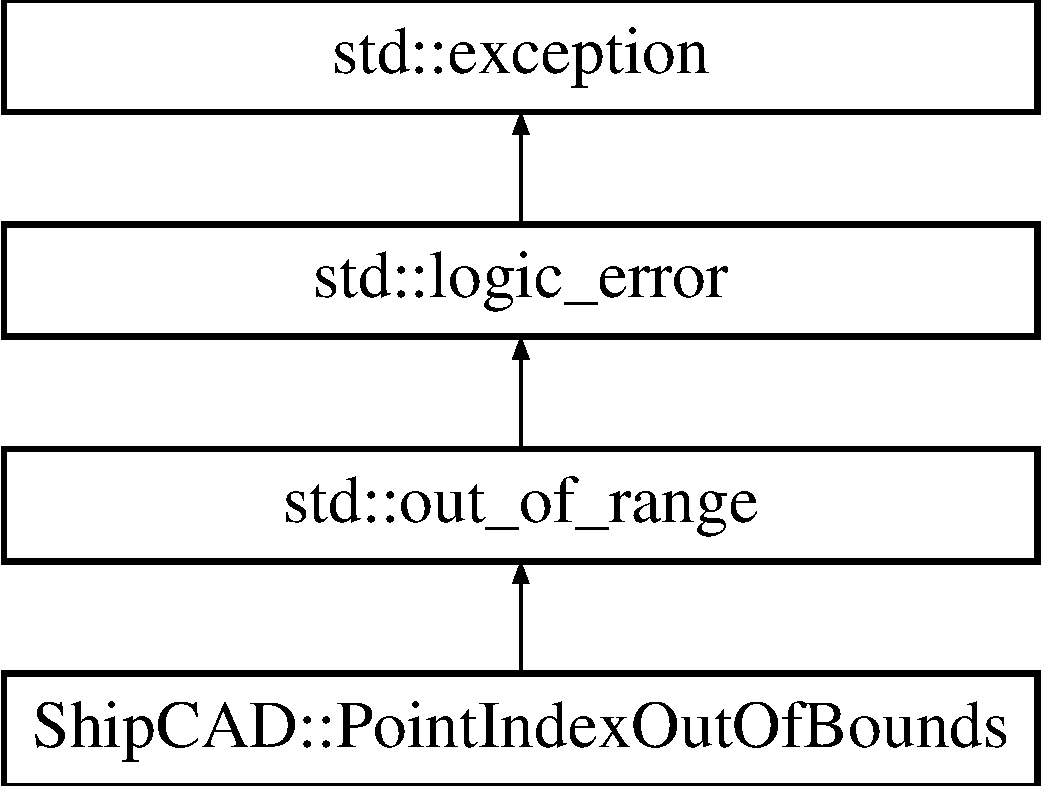
\includegraphics[height=4.000000cm]{classShipCAD_1_1PointIndexOutOfBounds}
\end{center}
\end{figure}
\subsection*{Public Member Functions}
\begin{DoxyCompactItemize}
\item 
\hyperlink{classShipCAD_1_1PointIndexOutOfBounds_a2bc663562d55642e627944582e20b283}{Point\-Index\-Out\-Of\-Bounds} (const std\-::string \&what\-\_\-arg)
\end{DoxyCompactItemize}


\subsection{Detailed Description}


Definition at line 44 of file exception.\-h.



\subsection{Constructor \& Destructor Documentation}
\hypertarget{classShipCAD_1_1PointIndexOutOfBounds_a2bc663562d55642e627944582e20b283}{\index{Ship\-C\-A\-D\-::\-Point\-Index\-Out\-Of\-Bounds@{Ship\-C\-A\-D\-::\-Point\-Index\-Out\-Of\-Bounds}!Point\-Index\-Out\-Of\-Bounds@{Point\-Index\-Out\-Of\-Bounds}}
\index{Point\-Index\-Out\-Of\-Bounds@{Point\-Index\-Out\-Of\-Bounds}!ShipCAD::PointIndexOutOfBounds@{Ship\-C\-A\-D\-::\-Point\-Index\-Out\-Of\-Bounds}}
\subsubsection[{Point\-Index\-Out\-Of\-Bounds}]{\setlength{\rightskip}{0pt plus 5cm}Ship\-C\-A\-D\-::\-Point\-Index\-Out\-Of\-Bounds\-::\-Point\-Index\-Out\-Of\-Bounds (
\begin{DoxyParamCaption}
\item[{const std\-::string \&}]{what\-\_\-arg}
\end{DoxyParamCaption}
)\hspace{0.3cm}{\ttfamily [inline]}}}\label{classShipCAD_1_1PointIndexOutOfBounds_a2bc663562d55642e627944582e20b283}


Definition at line 47 of file exception.\-h.



The documentation for this class was generated from the following file\-:\begin{DoxyCompactItemize}
\item 
Ship\-C\-A\-Dlib/\hyperlink{exception_8h}{exception.\-h}\end{DoxyCompactItemize}

\hypertarget{structPointPred}{\section{Point\-Pred Struct Reference}
\label{structPointPred}\index{Point\-Pred@{Point\-Pred}}
}
\subsection*{Public Member Functions}
\begin{DoxyCompactItemize}
\item 
bool \hyperlink{structPointPred_a3e2cfa1956feb6ddc90b9e48e52a241f}{operator()} (const pair$<$ \hyperlink{classShipCADGeometry_1_1SubdivisionPoint}{Ship\-C\-A\-D\-Geometry\-::\-Subdivision\-Point} $\ast$, \hyperlink{classShipCADGeometry_1_1SubdivisionPoint}{Ship\-C\-A\-D\-Geometry\-::\-Subdivision\-Point} $\ast$ $>$ \&val)
\item 
\hyperlink{structPointPred_aebfb99e471eb88c6abb630b2b0886c49}{Point\-Pred} (\hyperlink{classShipCADGeometry_1_1SubdivisionPoint}{Ship\-C\-A\-D\-Geometry\-::\-Subdivision\-Point} $\ast$querypt)
\end{DoxyCompactItemize}
\subsection*{Public Attributes}
\begin{DoxyCompactItemize}
\item 
\hyperlink{classShipCADGeometry_1_1SubdivisionPoint}{Ship\-C\-A\-D\-Geometry\-::\-Subdivision\-Point} $\ast$ \hyperlink{structPointPred_a44ee45b04c1d27518a0da3c19591d4b0}{\-\_\-querypt}
\end{DoxyCompactItemize}


\subsection{Detailed Description}


Definition at line 224 of file subdivface.\-cpp.



\subsection{Constructor \& Destructor Documentation}
\hypertarget{structPointPred_aebfb99e471eb88c6abb630b2b0886c49}{\index{Point\-Pred@{Point\-Pred}!Point\-Pred@{Point\-Pred}}
\index{Point\-Pred@{Point\-Pred}!PointPred@{Point\-Pred}}
\subsubsection[{Point\-Pred}]{\setlength{\rightskip}{0pt plus 5cm}Point\-Pred\-::\-Point\-Pred (
\begin{DoxyParamCaption}
\item[{{\bf Ship\-C\-A\-D\-Geometry\-::\-Subdivision\-Point} $\ast$}]{querypt}
\end{DoxyParamCaption}
)\hspace{0.3cm}{\ttfamily [inline]}}}\label{structPointPred_aebfb99e471eb88c6abb630b2b0886c49}


Definition at line 230 of file subdivface.\-cpp.



\subsection{Member Function Documentation}
\hypertarget{structPointPred_a3e2cfa1956feb6ddc90b9e48e52a241f}{\index{Point\-Pred@{Point\-Pred}!operator()@{operator()}}
\index{operator()@{operator()}!PointPred@{Point\-Pred}}
\subsubsection[{operator()}]{\setlength{\rightskip}{0pt plus 5cm}bool Point\-Pred\-::operator() (
\begin{DoxyParamCaption}
\item[{const pair$<$ {\bf Ship\-C\-A\-D\-Geometry\-::\-Subdivision\-Point} $\ast$, {\bf Ship\-C\-A\-D\-Geometry\-::\-Subdivision\-Point} $\ast$ $>$ \&}]{val}
\end{DoxyParamCaption}
)\hspace{0.3cm}{\ttfamily [inline]}}}\label{structPointPred_a3e2cfa1956feb6ddc90b9e48e52a241f}


Definition at line 226 of file subdivface.\-cpp.



\subsection{Member Data Documentation}
\hypertarget{structPointPred_a44ee45b04c1d27518a0da3c19591d4b0}{\index{Point\-Pred@{Point\-Pred}!\-\_\-querypt@{\-\_\-querypt}}
\index{\-\_\-querypt@{\-\_\-querypt}!PointPred@{Point\-Pred}}
\subsubsection[{\-\_\-querypt}]{\setlength{\rightskip}{0pt plus 5cm}{\bf Ship\-C\-A\-D\-Geometry\-::\-Subdivision\-Point}$\ast$ Point\-Pred\-::\-\_\-querypt}}\label{structPointPred_a44ee45b04c1d27518a0da3c19591d4b0}


Definition at line 225 of file subdivface.\-cpp.



The documentation for this struct was generated from the following file\-:\begin{DoxyCompactItemize}
\item 
Ship\-C\-A\-Dlib/\hyperlink{subdivface_8cpp}{subdivface.\-cpp}\end{DoxyCompactItemize}

\hypertarget{classShipCAD_1_1Preferences}{\section{Ship\-C\-A\-D\-:\-:Preferences Class Reference}
\label{classShipCAD_1_1Preferences}\index{Ship\-C\-A\-D\-::\-Preferences@{Ship\-C\-A\-D\-::\-Preferences}}
}


{\ttfamily \#include $<$preferences.\-h$>$}

Inheritance diagram for Ship\-C\-A\-D\-:\-:Preferences\-:\begin{figure}[H]
\begin{center}
\leavevmode
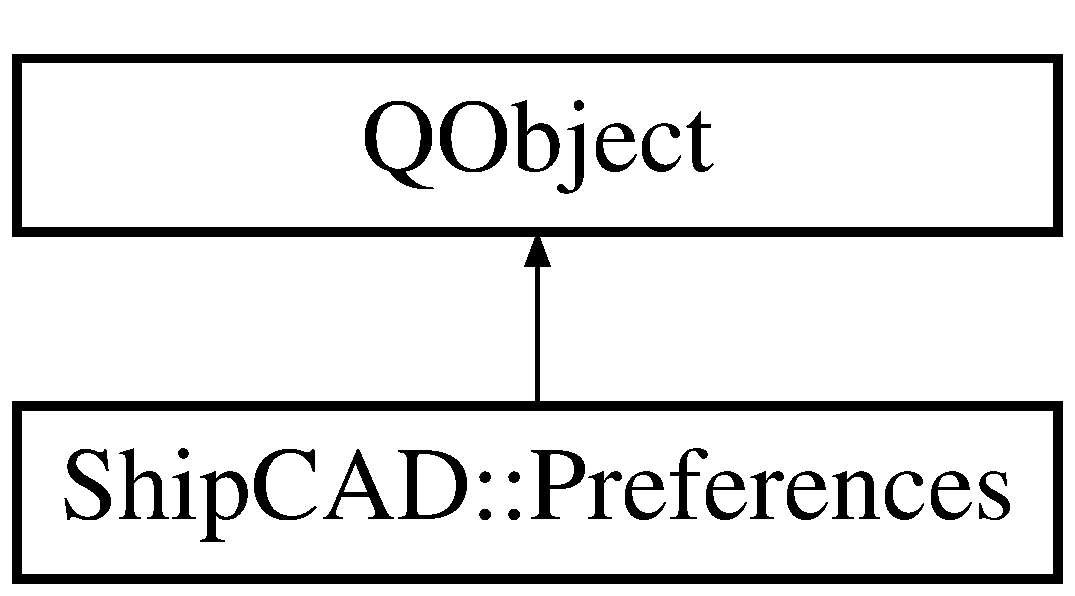
\includegraphics[height=2.000000cm]{classShipCAD_1_1Preferences}
\end{center}
\end{figure}
\subsection*{Public Member Functions}
\begin{DoxyCompactItemize}
\item 
\hyperlink{classShipCAD_1_1Preferences_afd469134e34b7e1982efeb1e402fce3b}{Preferences} (\hyperlink{classShipCAD_1_1ShipCADModel}{Ship\-C\-A\-D\-Model} $\ast$owner)
\item 
\hyperlink{classShipCAD_1_1Preferences_ab38e15f8965b1cd69b80369bb16a0995}{$\sim$\-Preferences} ()
\item 
Q\-String \hyperlink{classShipCAD_1_1Preferences_a9673a7bf93112ff78b6c8ca5d7cc3a4b}{get\-Export\-Directory} () const 
\item 
Q\-String \hyperlink{classShipCAD_1_1Preferences_a275aac8dc6e72c021ad00ff68f2fba54}{get\-Import\-Directory} () const 
\item 
Q\-String \hyperlink{classShipCAD_1_1Preferences_ab1ac99acb5ceb37b5cf7f6b21f376f27}{get\-Open\-Directory} () const 
\item 
Q\-String \hyperlink{classShipCAD_1_1Preferences_a5ee1cbf3c572b9253cfe958055e0eb43}{get\-Save\-Directory} () const 
\item 
void \hyperlink{classShipCAD_1_1Preferences_ad120b46e68a08d7682aaeb351b4c179d}{set\-Viewport\-Color} (Q\-Color col)
\item 
void \hyperlink{classShipCAD_1_1Preferences_a326180a1551596a3a9f2709d31c9fb10}{edit} ()
\item 
void \hyperlink{classShipCAD_1_1Preferences_a70c1b8f3b9e117d67c3cd50c33f66f3a}{load} ()
\item 
void \hyperlink{classShipCAD_1_1Preferences_a2e7e496b3417148240994e51281b0858}{reset\-Colors} ()
\item 
void \hyperlink{classShipCAD_1_1Preferences_ab3f40207c39fe262a7ae16ca22b297b2}{save} ()
\item 
size\-\_\-t \hyperlink{classShipCAD_1_1Preferences_a8ddfbabd8be21f6390f3750600047a87}{get\-Max\-Undo\-Memory} () const 
\begin{DoxyCompactList}\small\item\em get maximum amount of undo memory \end{DoxyCompactList}\item 
Q\-Color \hyperlink{classShipCAD_1_1Preferences_af54f177e516849e7f8212841db9b1ed8}{get\-Select\-Color} () const 
\item 
Q\-Color \hyperlink{classShipCAD_1_1Preferences_a39e4abd32055512f8009f4c8ab5cd379}{get\-Station\-Color} () const 
\item 
Q\-Color \hyperlink{classShipCAD_1_1Preferences_aa34f502af478c340ff359c76b90620c0}{get\-Buttock\-Color} () const 
\item 
Q\-Color \hyperlink{classShipCAD_1_1Preferences_a518043b34395026be6ebcf8f4e6e6591}{get\-Waterline\-Color} () const 
\item 
Q\-Color \hyperlink{classShipCAD_1_1Preferences_a238b56f29c89be9c2d9533cb9db21552}{get\-Diagonal\-Color} () const 
\item 
void \hyperlink{classShipCAD_1_1Preferences_ae2139f76ba4038b4e713ca75dcb8157e}{clear} ()
\end{DoxyCompactItemize}


\subsection{Detailed Description}


Definition at line 42 of file preferences.\-h.



\subsection{Constructor \& Destructor Documentation}
\hypertarget{classShipCAD_1_1Preferences_afd469134e34b7e1982efeb1e402fce3b}{\index{Ship\-C\-A\-D\-::\-Preferences@{Ship\-C\-A\-D\-::\-Preferences}!Preferences@{Preferences}}
\index{Preferences@{Preferences}!ShipCAD::Preferences@{Ship\-C\-A\-D\-::\-Preferences}}
\subsubsection[{Preferences}]{\setlength{\rightskip}{0pt plus 5cm}Preferences\-::\-Preferences (
\begin{DoxyParamCaption}
\item[{{\bf Ship\-C\-A\-D\-Model} $\ast$}]{owner}
\end{DoxyParamCaption}
)\hspace{0.3cm}{\ttfamily [explicit]}}}\label{classShipCAD_1_1Preferences_afd469134e34b7e1982efeb1e402fce3b}


Definition at line 35 of file preferences.\-cpp.

\hypertarget{classShipCAD_1_1Preferences_ab38e15f8965b1cd69b80369bb16a0995}{\index{Ship\-C\-A\-D\-::\-Preferences@{Ship\-C\-A\-D\-::\-Preferences}!$\sim$\-Preferences@{$\sim$\-Preferences}}
\index{$\sim$\-Preferences@{$\sim$\-Preferences}!ShipCAD::Preferences@{Ship\-C\-A\-D\-::\-Preferences}}
\subsubsection[{$\sim$\-Preferences}]{\setlength{\rightskip}{0pt plus 5cm}Ship\-C\-A\-D\-::\-Preferences\-::$\sim$\-Preferences (
\begin{DoxyParamCaption}
{}
\end{DoxyParamCaption}
)\hspace{0.3cm}{\ttfamily [inline]}}}\label{classShipCAD_1_1Preferences_ab38e15f8965b1cd69b80369bb16a0995}


Definition at line 48 of file preferences.\-h.



\subsection{Member Function Documentation}
\hypertarget{classShipCAD_1_1Preferences_ae2139f76ba4038b4e713ca75dcb8157e}{\index{Ship\-C\-A\-D\-::\-Preferences@{Ship\-C\-A\-D\-::\-Preferences}!clear@{clear}}
\index{clear@{clear}!ShipCAD::Preferences@{Ship\-C\-A\-D\-::\-Preferences}}
\subsubsection[{clear}]{\setlength{\rightskip}{0pt plus 5cm}void Preferences\-::clear (
\begin{DoxyParamCaption}
{}
\end{DoxyParamCaption}
)}}\label{classShipCAD_1_1Preferences_ae2139f76ba4038b4e713ca75dcb8157e}


Definition at line 41 of file preferences.\-cpp.

\hypertarget{classShipCAD_1_1Preferences_a326180a1551596a3a9f2709d31c9fb10}{\index{Ship\-C\-A\-D\-::\-Preferences@{Ship\-C\-A\-D\-::\-Preferences}!edit@{edit}}
\index{edit@{edit}!ShipCAD::Preferences@{Ship\-C\-A\-D\-::\-Preferences}}
\subsubsection[{edit}]{\setlength{\rightskip}{0pt plus 5cm}void Ship\-C\-A\-D\-::\-Preferences\-::edit (
\begin{DoxyParamCaption}
{}
\end{DoxyParamCaption}
)}}\label{classShipCAD_1_1Preferences_a326180a1551596a3a9f2709d31c9fb10}
\hypertarget{classShipCAD_1_1Preferences_aa34f502af478c340ff359c76b90620c0}{\index{Ship\-C\-A\-D\-::\-Preferences@{Ship\-C\-A\-D\-::\-Preferences}!get\-Buttock\-Color@{get\-Buttock\-Color}}
\index{get\-Buttock\-Color@{get\-Buttock\-Color}!ShipCAD::Preferences@{Ship\-C\-A\-D\-::\-Preferences}}
\subsubsection[{get\-Buttock\-Color}]{\setlength{\rightskip}{0pt plus 5cm}Q\-Color Ship\-C\-A\-D\-::\-Preferences\-::get\-Buttock\-Color (
\begin{DoxyParamCaption}
{}
\end{DoxyParamCaption}
) const\hspace{0.3cm}{\ttfamily [inline]}}}\label{classShipCAD_1_1Preferences_aa34f502af478c340ff359c76b90620c0}


Definition at line 73 of file preferences.\-h.

\hypertarget{classShipCAD_1_1Preferences_a238b56f29c89be9c2d9533cb9db21552}{\index{Ship\-C\-A\-D\-::\-Preferences@{Ship\-C\-A\-D\-::\-Preferences}!get\-Diagonal\-Color@{get\-Diagonal\-Color}}
\index{get\-Diagonal\-Color@{get\-Diagonal\-Color}!ShipCAD::Preferences@{Ship\-C\-A\-D\-::\-Preferences}}
\subsubsection[{get\-Diagonal\-Color}]{\setlength{\rightskip}{0pt plus 5cm}Q\-Color Ship\-C\-A\-D\-::\-Preferences\-::get\-Diagonal\-Color (
\begin{DoxyParamCaption}
{}
\end{DoxyParamCaption}
) const\hspace{0.3cm}{\ttfamily [inline]}}}\label{classShipCAD_1_1Preferences_a238b56f29c89be9c2d9533cb9db21552}


Definition at line 77 of file preferences.\-h.

\hypertarget{classShipCAD_1_1Preferences_a9673a7bf93112ff78b6c8ca5d7cc3a4b}{\index{Ship\-C\-A\-D\-::\-Preferences@{Ship\-C\-A\-D\-::\-Preferences}!get\-Export\-Directory@{get\-Export\-Directory}}
\index{get\-Export\-Directory@{get\-Export\-Directory}!ShipCAD::Preferences@{Ship\-C\-A\-D\-::\-Preferences}}
\subsubsection[{get\-Export\-Directory}]{\setlength{\rightskip}{0pt plus 5cm}Q\-String Ship\-C\-A\-D\-::\-Preferences\-::get\-Export\-Directory (
\begin{DoxyParamCaption}
{}
\end{DoxyParamCaption}
) const}}\label{classShipCAD_1_1Preferences_a9673a7bf93112ff78b6c8ca5d7cc3a4b}
\hypertarget{classShipCAD_1_1Preferences_a275aac8dc6e72c021ad00ff68f2fba54}{\index{Ship\-C\-A\-D\-::\-Preferences@{Ship\-C\-A\-D\-::\-Preferences}!get\-Import\-Directory@{get\-Import\-Directory}}
\index{get\-Import\-Directory@{get\-Import\-Directory}!ShipCAD::Preferences@{Ship\-C\-A\-D\-::\-Preferences}}
\subsubsection[{get\-Import\-Directory}]{\setlength{\rightskip}{0pt plus 5cm}Q\-String Ship\-C\-A\-D\-::\-Preferences\-::get\-Import\-Directory (
\begin{DoxyParamCaption}
{}
\end{DoxyParamCaption}
) const}}\label{classShipCAD_1_1Preferences_a275aac8dc6e72c021ad00ff68f2fba54}
\hypertarget{classShipCAD_1_1Preferences_a8ddfbabd8be21f6390f3750600047a87}{\index{Ship\-C\-A\-D\-::\-Preferences@{Ship\-C\-A\-D\-::\-Preferences}!get\-Max\-Undo\-Memory@{get\-Max\-Undo\-Memory}}
\index{get\-Max\-Undo\-Memory@{get\-Max\-Undo\-Memory}!ShipCAD::Preferences@{Ship\-C\-A\-D\-::\-Preferences}}
\subsubsection[{get\-Max\-Undo\-Memory}]{\setlength{\rightskip}{0pt plus 5cm}size\-\_\-t Ship\-C\-A\-D\-::\-Preferences\-::get\-Max\-Undo\-Memory (
\begin{DoxyParamCaption}
{}
\end{DoxyParamCaption}
) const\hspace{0.3cm}{\ttfamily [inline]}}}\label{classShipCAD_1_1Preferences_a8ddfbabd8be21f6390f3750600047a87}


get maximum amount of undo memory 

\begin{DoxyReturn}{Returns}
max amount of undo memory in mb 
\end{DoxyReturn}


Definition at line 66 of file preferences.\-h.

\hypertarget{classShipCAD_1_1Preferences_ab1ac99acb5ceb37b5cf7f6b21f376f27}{\index{Ship\-C\-A\-D\-::\-Preferences@{Ship\-C\-A\-D\-::\-Preferences}!get\-Open\-Directory@{get\-Open\-Directory}}
\index{get\-Open\-Directory@{get\-Open\-Directory}!ShipCAD::Preferences@{Ship\-C\-A\-D\-::\-Preferences}}
\subsubsection[{get\-Open\-Directory}]{\setlength{\rightskip}{0pt plus 5cm}Q\-String Ship\-C\-A\-D\-::\-Preferences\-::get\-Open\-Directory (
\begin{DoxyParamCaption}
{}
\end{DoxyParamCaption}
) const}}\label{classShipCAD_1_1Preferences_ab1ac99acb5ceb37b5cf7f6b21f376f27}
\hypertarget{classShipCAD_1_1Preferences_a5ee1cbf3c572b9253cfe958055e0eb43}{\index{Ship\-C\-A\-D\-::\-Preferences@{Ship\-C\-A\-D\-::\-Preferences}!get\-Save\-Directory@{get\-Save\-Directory}}
\index{get\-Save\-Directory@{get\-Save\-Directory}!ShipCAD::Preferences@{Ship\-C\-A\-D\-::\-Preferences}}
\subsubsection[{get\-Save\-Directory}]{\setlength{\rightskip}{0pt plus 5cm}Q\-String Ship\-C\-A\-D\-::\-Preferences\-::get\-Save\-Directory (
\begin{DoxyParamCaption}
{}
\end{DoxyParamCaption}
) const}}\label{classShipCAD_1_1Preferences_a5ee1cbf3c572b9253cfe958055e0eb43}
\hypertarget{classShipCAD_1_1Preferences_af54f177e516849e7f8212841db9b1ed8}{\index{Ship\-C\-A\-D\-::\-Preferences@{Ship\-C\-A\-D\-::\-Preferences}!get\-Select\-Color@{get\-Select\-Color}}
\index{get\-Select\-Color@{get\-Select\-Color}!ShipCAD::Preferences@{Ship\-C\-A\-D\-::\-Preferences}}
\subsubsection[{get\-Select\-Color}]{\setlength{\rightskip}{0pt plus 5cm}Q\-Color Ship\-C\-A\-D\-::\-Preferences\-::get\-Select\-Color (
\begin{DoxyParamCaption}
{}
\end{DoxyParamCaption}
) const\hspace{0.3cm}{\ttfamily [inline]}}}\label{classShipCAD_1_1Preferences_af54f177e516849e7f8212841db9b1ed8}


Definition at line 69 of file preferences.\-h.

\hypertarget{classShipCAD_1_1Preferences_a39e4abd32055512f8009f4c8ab5cd379}{\index{Ship\-C\-A\-D\-::\-Preferences@{Ship\-C\-A\-D\-::\-Preferences}!get\-Station\-Color@{get\-Station\-Color}}
\index{get\-Station\-Color@{get\-Station\-Color}!ShipCAD::Preferences@{Ship\-C\-A\-D\-::\-Preferences}}
\subsubsection[{get\-Station\-Color}]{\setlength{\rightskip}{0pt plus 5cm}Q\-Color Ship\-C\-A\-D\-::\-Preferences\-::get\-Station\-Color (
\begin{DoxyParamCaption}
{}
\end{DoxyParamCaption}
) const\hspace{0.3cm}{\ttfamily [inline]}}}\label{classShipCAD_1_1Preferences_a39e4abd32055512f8009f4c8ab5cd379}


Definition at line 71 of file preferences.\-h.

\hypertarget{classShipCAD_1_1Preferences_a518043b34395026be6ebcf8f4e6e6591}{\index{Ship\-C\-A\-D\-::\-Preferences@{Ship\-C\-A\-D\-::\-Preferences}!get\-Waterline\-Color@{get\-Waterline\-Color}}
\index{get\-Waterline\-Color@{get\-Waterline\-Color}!ShipCAD::Preferences@{Ship\-C\-A\-D\-::\-Preferences}}
\subsubsection[{get\-Waterline\-Color}]{\setlength{\rightskip}{0pt plus 5cm}Q\-Color Ship\-C\-A\-D\-::\-Preferences\-::get\-Waterline\-Color (
\begin{DoxyParamCaption}
{}
\end{DoxyParamCaption}
) const\hspace{0.3cm}{\ttfamily [inline]}}}\label{classShipCAD_1_1Preferences_a518043b34395026be6ebcf8f4e6e6591}


Definition at line 75 of file preferences.\-h.

\hypertarget{classShipCAD_1_1Preferences_a70c1b8f3b9e117d67c3cd50c33f66f3a}{\index{Ship\-C\-A\-D\-::\-Preferences@{Ship\-C\-A\-D\-::\-Preferences}!load@{load}}
\index{load@{load}!ShipCAD::Preferences@{Ship\-C\-A\-D\-::\-Preferences}}
\subsubsection[{load}]{\setlength{\rightskip}{0pt plus 5cm}void Ship\-C\-A\-D\-::\-Preferences\-::load (
\begin{DoxyParamCaption}
{}
\end{DoxyParamCaption}
)}}\label{classShipCAD_1_1Preferences_a70c1b8f3b9e117d67c3cd50c33f66f3a}
\hypertarget{classShipCAD_1_1Preferences_a2e7e496b3417148240994e51281b0858}{\index{Ship\-C\-A\-D\-::\-Preferences@{Ship\-C\-A\-D\-::\-Preferences}!reset\-Colors@{reset\-Colors}}
\index{reset\-Colors@{reset\-Colors}!ShipCAD::Preferences@{Ship\-C\-A\-D\-::\-Preferences}}
\subsubsection[{reset\-Colors}]{\setlength{\rightskip}{0pt plus 5cm}void Preferences\-::reset\-Colors (
\begin{DoxyParamCaption}
{}
\end{DoxyParamCaption}
)}}\label{classShipCAD_1_1Preferences_a2e7e496b3417148240994e51281b0858}


Definition at line 48 of file preferences.\-cpp.

\hypertarget{classShipCAD_1_1Preferences_ab3f40207c39fe262a7ae16ca22b297b2}{\index{Ship\-C\-A\-D\-::\-Preferences@{Ship\-C\-A\-D\-::\-Preferences}!save@{save}}
\index{save@{save}!ShipCAD::Preferences@{Ship\-C\-A\-D\-::\-Preferences}}
\subsubsection[{save}]{\setlength{\rightskip}{0pt plus 5cm}void Ship\-C\-A\-D\-::\-Preferences\-::save (
\begin{DoxyParamCaption}
{}
\end{DoxyParamCaption}
)}}\label{classShipCAD_1_1Preferences_ab3f40207c39fe262a7ae16ca22b297b2}
\hypertarget{classShipCAD_1_1Preferences_ad120b46e68a08d7682aaeb351b4c179d}{\index{Ship\-C\-A\-D\-::\-Preferences@{Ship\-C\-A\-D\-::\-Preferences}!set\-Viewport\-Color@{set\-Viewport\-Color}}
\index{set\-Viewport\-Color@{set\-Viewport\-Color}!ShipCAD::Preferences@{Ship\-C\-A\-D\-::\-Preferences}}
\subsubsection[{set\-Viewport\-Color}]{\setlength{\rightskip}{0pt plus 5cm}void Ship\-C\-A\-D\-::\-Preferences\-::set\-Viewport\-Color (
\begin{DoxyParamCaption}
\item[{Q\-Color}]{col}
\end{DoxyParamCaption}
)}}\label{classShipCAD_1_1Preferences_ad120b46e68a08d7682aaeb351b4c179d}


The documentation for this class was generated from the following files\-:\begin{DoxyCompactItemize}
\item 
Ship\-C\-A\-Dlib/\hyperlink{preferences_8h}{preferences.\-h}\item 
Ship\-C\-A\-Dlib/\hyperlink{preferences_8cpp}{preferences.\-cpp}\end{DoxyCompactItemize}

\hypertarget{classShipCAD_1_1ProjectSettings}{\section{Ship\-C\-A\-D\-:\-:Project\-Settings Class Reference}
\label{classShipCAD_1_1ProjectSettings}\index{Ship\-C\-A\-D\-::\-Project\-Settings@{Ship\-C\-A\-D\-::\-Project\-Settings}}
}


{\ttfamily \#include $<$projsettings.\-h$>$}

Inheritance diagram for Ship\-C\-A\-D\-:\-:Project\-Settings\-:\begin{figure}[H]
\begin{center}
\leavevmode
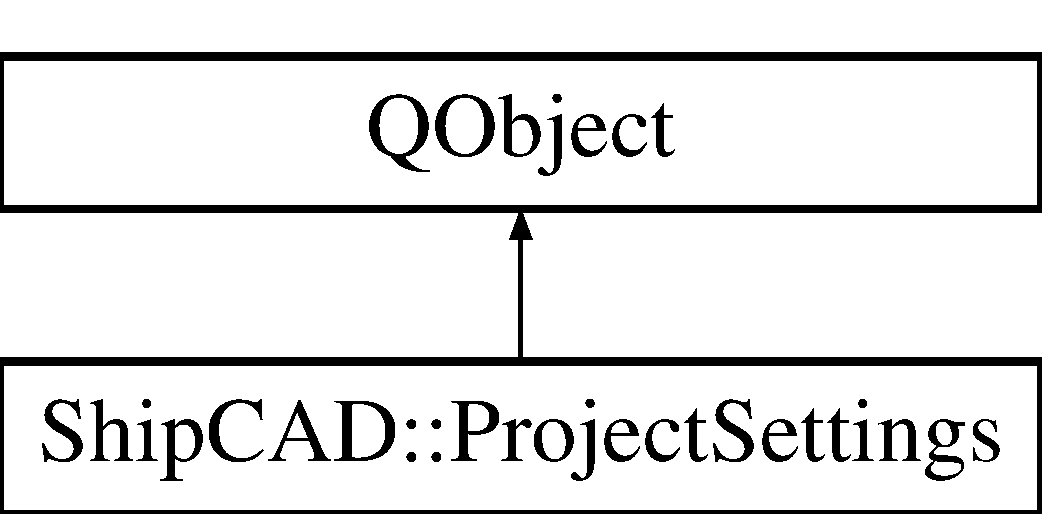
\includegraphics[height=2.000000cm]{classShipCAD_1_1ProjectSettings}
\end{center}
\end{figure}
\subsection*{Public Member Functions}
\begin{DoxyCompactItemize}
\item 
\hyperlink{classShipCAD_1_1ProjectSettings_a55001252531c21f4ccc89d8df9c6b184}{Project\-Settings} (\hyperlink{classShipCAD_1_1ShipCADModel}{Ship\-C\-A\-D\-Model} $\ast$owner)
\item 
\hyperlink{classShipCAD_1_1ProjectSettings_a4c74ba587e58e538083072285937aa4c}{$\sim$\-Project\-Settings} ()
\item 
\hyperlink{namespaceShipCAD_a9cf77f0900561de9efc572dcbad4dbbd}{hydrostatic\-\_\-coeff\-\_\-t} \hyperlink{classShipCAD_1_1ProjectSettings_aef0458c7bfa6e484a155e78eca0d0202}{get\-Hydrostatic\-Coefficients} ()
\item 
void \hyperlink{classShipCAD_1_1ProjectSettings_ab729e778076b560d876f09955212256d}{set\-Hydrostatic\-Coefficients} (\hyperlink{namespaceShipCAD_a9cf77f0900561de9efc572dcbad4dbbd}{hydrostatic\-\_\-coeff\-\_\-t} coeff)
\item 
void \hyperlink{classShipCAD_1_1ProjectSettings_ab9f9f88bba11a2093204affd18df17ab}{set\-Disable\-Model\-Check} (bool val)
\item 
float \hyperlink{classShipCAD_1_1ProjectSettings_a4dddaf7fe8bdbc0724c524244dd56497}{get\-Mainframe\-Location} ()
\item 
float \hyperlink{classShipCAD_1_1ProjectSettings_ada67c18ca75cb78d5591f24dcaf88b31}{get\-Appendage\-Coefficient} ()
\item 
void \hyperlink{classShipCAD_1_1ProjectSettings_a31fdcc5990fb3c61161fe783b5ed4939}{set\-Appendage\-Coefficient} (float coeff)
\item 
float \hyperlink{classShipCAD_1_1ProjectSettings_a451c6b10193f54fa76e9857005e31e61}{get\-Beam} ()
\item 
void \hyperlink{classShipCAD_1_1ProjectSettings_ac90d2a093ae0af951fd117d7f6981e92}{set\-Beam} (float beam)
\item 
void \hyperlink{classShipCAD_1_1ProjectSettings_a16a64f2a4a9b6359ac46b0a85f90a4ae}{set\-Draft} (float draft)
\item 
float \hyperlink{classShipCAD_1_1ProjectSettings_a989e357d35af68ac2da9b0e760926308}{get\-Length} ()
\item 
void \hyperlink{classShipCAD_1_1ProjectSettings_aad72cb11575e7a1ae0cda2c50f8de2ad}{set\-Length} (float length)
\item 
void \hyperlink{classShipCAD_1_1ProjectSettings_acac72dbc1dc2f68c1d32981ac9a27603}{set\-Mainframe\-Location} (float loc)
\item 
float \hyperlink{classShipCAD_1_1ProjectSettings_a8a0cffbd479739406500541a7d896d4a}{get\-Water\-Density} ()
\item 
void \hyperlink{classShipCAD_1_1ProjectSettings_af4de74cc452581cf8f7e02431ba3e45a}{set\-Water\-Density} (float val)
\item 
void \hyperlink{classShipCAD_1_1ProjectSettings_a3590a9b52236a4aeb9991ea03c518871}{set\-Save\-Preview} (bool val)
\item 
void \hyperlink{classShipCAD_1_1ProjectSettings_a9e389573e2266b099f49452d68edf24f}{set\-Start\-Draft} (float val)
\item 
void \hyperlink{classShipCAD_1_1ProjectSettings_afdab155f3ca324b3c200a97c9ade1ff6}{set\-Trim} (float val)
\item 
void \hyperlink{classShipCAD_1_1ProjectSettings_a45e70a08ac47cdf30971a7386af702a9}{set\-End\-Draft} (float val)
\item 
void \hyperlink{classShipCAD_1_1ProjectSettings_a45081194c5e105780429b0f214bab186}{set\-Draft\-Step} (float val)
\item 
void \hyperlink{classShipCAD_1_1ProjectSettings_a7c0f0e54fb2fb94a70b823fca6a6a58d}{set\-Use\-Default\-Mainframe\-Location} (bool use)
\item 
void \hyperlink{classShipCAD_1_1ProjectSettings_acaa6149ff4c93c829a72a3a3d2ff5239}{set\-Name} (const Q\-String \&name)
\item 
void \hyperlink{classShipCAD_1_1ProjectSettings_abde123a71eba642ff1dbd62d547aa684}{set\-Designer} (const Q\-String \&designer)
\item 
void \hyperlink{classShipCAD_1_1ProjectSettings_a64e942847dd0838f04dc4ec32e9bc30e}{set\-Comment} (const Q\-String \&comment)
\item 
void \hyperlink{classShipCAD_1_1ProjectSettings_a326e18ff53ba0f916d4d8cfab5a2d17f}{set\-File\-Created\-By} (const Q\-String \&createdby)
\item 
void \hyperlink{classShipCAD_1_1ProjectSettings_a0f40362f42e6dfd4147d69573c00988f}{set\-Shade\-Underwater\-Ship} (bool set)
\item 
bool \hyperlink{classShipCAD_1_1ProjectSettings_a2e5f2bfb546885af0af8d857198b8cc9}{get\-Simplify\-Intersections} ()
\item 
void \hyperlink{classShipCAD_1_1ProjectSettings_a138264f53da99f6a1765ea7aec95096a}{set\-Simplify\-Intersections} (bool set)
\item 
void \hyperlink{classShipCAD_1_1ProjectSettings_a06b1260b284a988fb62b49f7ab4d5bf3}{set\-Under\-Water\-Color} (Q\-Color \&col)
\item 
\hyperlink{namespaceShipCAD_ac6a7a28b4b063771afae92decb602da5}{unit\-\_\-type\-\_\-t} \hyperlink{classShipCAD_1_1ProjectSettings_a604a1aea4c17269f290e06ae51a0051c}{get\-Units} ()
\item 
void \hyperlink{classShipCAD_1_1ProjectSettings_a2310573735d3c0ad17ca290bca083f99}{set\-Units} (\hyperlink{namespaceShipCAD_ac6a7a28b4b063771afae92decb602da5}{unit\-\_\-type\-\_\-t} unit)
\item 
void \hyperlink{classShipCAD_1_1ProjectSettings_af6012d62299292d0757955b14c6bd854}{load\-Binary} (\hyperlink{classShipCAD_1_1FileBuffer}{File\-Buffer} \&source, Q\-Image $\ast$img)
\item 
void \hyperlink{classShipCAD_1_1ProjectSettings_aebda4677da789819020d1ea1623ec035}{save\-Binary} (\hyperlink{classShipCAD_1_1FileBuffer}{File\-Buffer} \&dest)
\item 
void \hyperlink{classShipCAD_1_1ProjectSettings_a9e0ce44e6aea8e57608baee2a3b05827}{clear} ()
\item 
void \hyperlink{classShipCAD_1_1ProjectSettings_a9caa9e15bc03de5b6092c419a58a87e8}{dump} (std\-::ostream \&os) const 
\end{DoxyCompactItemize}


\subsection{Detailed Description}


Definition at line 46 of file projsettings.\-h.



\subsection{Constructor \& Destructor Documentation}
\hypertarget{classShipCAD_1_1ProjectSettings_a55001252531c21f4ccc89d8df9c6b184}{\index{Ship\-C\-A\-D\-::\-Project\-Settings@{Ship\-C\-A\-D\-::\-Project\-Settings}!Project\-Settings@{Project\-Settings}}
\index{Project\-Settings@{Project\-Settings}!ShipCAD::ProjectSettings@{Ship\-C\-A\-D\-::\-Project\-Settings}}
\subsubsection[{Project\-Settings}]{\setlength{\rightskip}{0pt plus 5cm}Project\-Settings\-::\-Project\-Settings (
\begin{DoxyParamCaption}
\item[{{\bf Ship\-C\-A\-D\-Model} $\ast$}]{owner}
\end{DoxyParamCaption}
)\hspace{0.3cm}{\ttfamily [explicit]}}}\label{classShipCAD_1_1ProjectSettings_a55001252531c21f4ccc89d8df9c6b184}


Definition at line 45 of file projsettings.\-cpp.

\hypertarget{classShipCAD_1_1ProjectSettings_a4c74ba587e58e538083072285937aa4c}{\index{Ship\-C\-A\-D\-::\-Project\-Settings@{Ship\-C\-A\-D\-::\-Project\-Settings}!$\sim$\-Project\-Settings@{$\sim$\-Project\-Settings}}
\index{$\sim$\-Project\-Settings@{$\sim$\-Project\-Settings}!ShipCAD::ProjectSettings@{Ship\-C\-A\-D\-::\-Project\-Settings}}
\subsubsection[{$\sim$\-Project\-Settings}]{\setlength{\rightskip}{0pt plus 5cm}Project\-Settings\-::$\sim$\-Project\-Settings (
\begin{DoxyParamCaption}
{}
\end{DoxyParamCaption}
)}}\label{classShipCAD_1_1ProjectSettings_a4c74ba587e58e538083072285937aa4c}


Definition at line 51 of file projsettings.\-cpp.



\subsection{Member Function Documentation}
\hypertarget{classShipCAD_1_1ProjectSettings_a9e0ce44e6aea8e57608baee2a3b05827}{\index{Ship\-C\-A\-D\-::\-Project\-Settings@{Ship\-C\-A\-D\-::\-Project\-Settings}!clear@{clear}}
\index{clear@{clear}!ShipCAD::ProjectSettings@{Ship\-C\-A\-D\-::\-Project\-Settings}}
\subsubsection[{clear}]{\setlength{\rightskip}{0pt plus 5cm}void Project\-Settings\-::clear (
\begin{DoxyParamCaption}
{}
\end{DoxyParamCaption}
)}}\label{classShipCAD_1_1ProjectSettings_a9e0ce44e6aea8e57608baee2a3b05827}


Definition at line 271 of file projsettings.\-cpp.

\hypertarget{classShipCAD_1_1ProjectSettings_a9caa9e15bc03de5b6092c419a58a87e8}{\index{Ship\-C\-A\-D\-::\-Project\-Settings@{Ship\-C\-A\-D\-::\-Project\-Settings}!dump@{dump}}
\index{dump@{dump}!ShipCAD::ProjectSettings@{Ship\-C\-A\-D\-::\-Project\-Settings}}
\subsubsection[{dump}]{\setlength{\rightskip}{0pt plus 5cm}void Project\-Settings\-::dump (
\begin{DoxyParamCaption}
\item[{std\-::ostream \&}]{os}
\end{DoxyParamCaption}
) const}}\label{classShipCAD_1_1ProjectSettings_a9caa9e15bc03de5b6092c419a58a87e8}


Definition at line 388 of file projsettings.\-cpp.

\hypertarget{classShipCAD_1_1ProjectSettings_ada67c18ca75cb78d5591f24dcaf88b31}{\index{Ship\-C\-A\-D\-::\-Project\-Settings@{Ship\-C\-A\-D\-::\-Project\-Settings}!get\-Appendage\-Coefficient@{get\-Appendage\-Coefficient}}
\index{get\-Appendage\-Coefficient@{get\-Appendage\-Coefficient}!ShipCAD::ProjectSettings@{Ship\-C\-A\-D\-::\-Project\-Settings}}
\subsubsection[{get\-Appendage\-Coefficient}]{\setlength{\rightskip}{0pt plus 5cm}float Ship\-C\-A\-D\-::\-Project\-Settings\-::get\-Appendage\-Coefficient (
\begin{DoxyParamCaption}
{}
\end{DoxyParamCaption}
)}}\label{classShipCAD_1_1ProjectSettings_ada67c18ca75cb78d5591f24dcaf88b31}
\hypertarget{classShipCAD_1_1ProjectSettings_a451c6b10193f54fa76e9857005e31e61}{\index{Ship\-C\-A\-D\-::\-Project\-Settings@{Ship\-C\-A\-D\-::\-Project\-Settings}!get\-Beam@{get\-Beam}}
\index{get\-Beam@{get\-Beam}!ShipCAD::ProjectSettings@{Ship\-C\-A\-D\-::\-Project\-Settings}}
\subsubsection[{get\-Beam}]{\setlength{\rightskip}{0pt plus 5cm}float Ship\-C\-A\-D\-::\-Project\-Settings\-::get\-Beam (
\begin{DoxyParamCaption}
{}
\end{DoxyParamCaption}
)}}\label{classShipCAD_1_1ProjectSettings_a451c6b10193f54fa76e9857005e31e61}
\hypertarget{classShipCAD_1_1ProjectSettings_aef0458c7bfa6e484a155e78eca0d0202}{\index{Ship\-C\-A\-D\-::\-Project\-Settings@{Ship\-C\-A\-D\-::\-Project\-Settings}!get\-Hydrostatic\-Coefficients@{get\-Hydrostatic\-Coefficients}}
\index{get\-Hydrostatic\-Coefficients@{get\-Hydrostatic\-Coefficients}!ShipCAD::ProjectSettings@{Ship\-C\-A\-D\-::\-Project\-Settings}}
\subsubsection[{get\-Hydrostatic\-Coefficients}]{\setlength{\rightskip}{0pt plus 5cm}{\bf hydrostatic\-\_\-coeff\-\_\-t} Ship\-C\-A\-D\-::\-Project\-Settings\-::get\-Hydrostatic\-Coefficients (
\begin{DoxyParamCaption}
{}
\end{DoxyParamCaption}
)}}\label{classShipCAD_1_1ProjectSettings_aef0458c7bfa6e484a155e78eca0d0202}
\hypertarget{classShipCAD_1_1ProjectSettings_a989e357d35af68ac2da9b0e760926308}{\index{Ship\-C\-A\-D\-::\-Project\-Settings@{Ship\-C\-A\-D\-::\-Project\-Settings}!get\-Length@{get\-Length}}
\index{get\-Length@{get\-Length}!ShipCAD::ProjectSettings@{Ship\-C\-A\-D\-::\-Project\-Settings}}
\subsubsection[{get\-Length}]{\setlength{\rightskip}{0pt plus 5cm}float Ship\-C\-A\-D\-::\-Project\-Settings\-::get\-Length (
\begin{DoxyParamCaption}
{}
\end{DoxyParamCaption}
)\hspace{0.3cm}{\ttfamily [inline]}}}\label{classShipCAD_1_1ProjectSettings_a989e357d35af68ac2da9b0e760926308}


Definition at line 63 of file projsettings.\-h.

\hypertarget{classShipCAD_1_1ProjectSettings_a4dddaf7fe8bdbc0724c524244dd56497}{\index{Ship\-C\-A\-D\-::\-Project\-Settings@{Ship\-C\-A\-D\-::\-Project\-Settings}!get\-Mainframe\-Location@{get\-Mainframe\-Location}}
\index{get\-Mainframe\-Location@{get\-Mainframe\-Location}!ShipCAD::ProjectSettings@{Ship\-C\-A\-D\-::\-Project\-Settings}}
\subsubsection[{get\-Mainframe\-Location}]{\setlength{\rightskip}{0pt plus 5cm}float Project\-Settings\-::get\-Mainframe\-Location (
\begin{DoxyParamCaption}
{}
\end{DoxyParamCaption}
)}}\label{classShipCAD_1_1ProjectSettings_a4dddaf7fe8bdbc0724c524244dd56497}


Definition at line 77 of file projsettings.\-cpp.

\hypertarget{classShipCAD_1_1ProjectSettings_a2e5f2bfb546885af0af8d857198b8cc9}{\index{Ship\-C\-A\-D\-::\-Project\-Settings@{Ship\-C\-A\-D\-::\-Project\-Settings}!get\-Simplify\-Intersections@{get\-Simplify\-Intersections}}
\index{get\-Simplify\-Intersections@{get\-Simplify\-Intersections}!ShipCAD::ProjectSettings@{Ship\-C\-A\-D\-::\-Project\-Settings}}
\subsubsection[{get\-Simplify\-Intersections}]{\setlength{\rightskip}{0pt plus 5cm}bool Ship\-C\-A\-D\-::\-Project\-Settings\-::get\-Simplify\-Intersections (
\begin{DoxyParamCaption}
{}
\end{DoxyParamCaption}
)\hspace{0.3cm}{\ttfamily [inline]}}}\label{classShipCAD_1_1ProjectSettings_a2e5f2bfb546885af0af8d857198b8cc9}


Definition at line 79 of file projsettings.\-h.

\hypertarget{classShipCAD_1_1ProjectSettings_a604a1aea4c17269f290e06ae51a0051c}{\index{Ship\-C\-A\-D\-::\-Project\-Settings@{Ship\-C\-A\-D\-::\-Project\-Settings}!get\-Units@{get\-Units}}
\index{get\-Units@{get\-Units}!ShipCAD::ProjectSettings@{Ship\-C\-A\-D\-::\-Project\-Settings}}
\subsubsection[{get\-Units}]{\setlength{\rightskip}{0pt plus 5cm}{\bf unit\-\_\-type\-\_\-t} Ship\-C\-A\-D\-::\-Project\-Settings\-::get\-Units (
\begin{DoxyParamCaption}
{}
\end{DoxyParamCaption}
)}}\label{classShipCAD_1_1ProjectSettings_a604a1aea4c17269f290e06ae51a0051c}
\hypertarget{classShipCAD_1_1ProjectSettings_a8a0cffbd479739406500541a7d896d4a}{\index{Ship\-C\-A\-D\-::\-Project\-Settings@{Ship\-C\-A\-D\-::\-Project\-Settings}!get\-Water\-Density@{get\-Water\-Density}}
\index{get\-Water\-Density@{get\-Water\-Density}!ShipCAD::ProjectSettings@{Ship\-C\-A\-D\-::\-Project\-Settings}}
\subsubsection[{get\-Water\-Density}]{\setlength{\rightskip}{0pt plus 5cm}float Ship\-C\-A\-D\-::\-Project\-Settings\-::get\-Water\-Density (
\begin{DoxyParamCaption}
{}
\end{DoxyParamCaption}
)}}\label{classShipCAD_1_1ProjectSettings_a8a0cffbd479739406500541a7d896d4a}
\hypertarget{classShipCAD_1_1ProjectSettings_af6012d62299292d0757955b14c6bd854}{\index{Ship\-C\-A\-D\-::\-Project\-Settings@{Ship\-C\-A\-D\-::\-Project\-Settings}!load\-Binary@{load\-Binary}}
\index{load\-Binary@{load\-Binary}!ShipCAD::ProjectSettings@{Ship\-C\-A\-D\-::\-Project\-Settings}}
\subsubsection[{load\-Binary}]{\setlength{\rightskip}{0pt plus 5cm}void Project\-Settings\-::load\-Binary (
\begin{DoxyParamCaption}
\item[{{\bf File\-Buffer} \&}]{source, }
\item[{Q\-Image $\ast$}]{img}
\end{DoxyParamCaption}
)}}\label{classShipCAD_1_1ProjectSettings_af6012d62299292d0757955b14c6bd854}


Definition at line 318 of file projsettings.\-cpp.

\hypertarget{classShipCAD_1_1ProjectSettings_aebda4677da789819020d1ea1623ec035}{\index{Ship\-C\-A\-D\-::\-Project\-Settings@{Ship\-C\-A\-D\-::\-Project\-Settings}!save\-Binary@{save\-Binary}}
\index{save\-Binary@{save\-Binary}!ShipCAD::ProjectSettings@{Ship\-C\-A\-D\-::\-Project\-Settings}}
\subsubsection[{save\-Binary}]{\setlength{\rightskip}{0pt plus 5cm}void Project\-Settings\-::save\-Binary (
\begin{DoxyParamCaption}
\item[{{\bf File\-Buffer} \&}]{dest}
\end{DoxyParamCaption}
)}}\label{classShipCAD_1_1ProjectSettings_aebda4677da789819020d1ea1623ec035}


Definition at line 383 of file projsettings.\-cpp.

\hypertarget{classShipCAD_1_1ProjectSettings_a31fdcc5990fb3c61161fe783b5ed4939}{\index{Ship\-C\-A\-D\-::\-Project\-Settings@{Ship\-C\-A\-D\-::\-Project\-Settings}!set\-Appendage\-Coefficient@{set\-Appendage\-Coefficient}}
\index{set\-Appendage\-Coefficient@{set\-Appendage\-Coefficient}!ShipCAD::ProjectSettings@{Ship\-C\-A\-D\-::\-Project\-Settings}}
\subsubsection[{set\-Appendage\-Coefficient}]{\setlength{\rightskip}{0pt plus 5cm}void Project\-Settings\-::set\-Appendage\-Coefficient (
\begin{DoxyParamCaption}
\item[{float}]{coeff}
\end{DoxyParamCaption}
)}}\label{classShipCAD_1_1ProjectSettings_a31fdcc5990fb3c61161fe783b5ed4939}


Definition at line 85 of file projsettings.\-cpp.

\hypertarget{classShipCAD_1_1ProjectSettings_ac90d2a093ae0af951fd117d7f6981e92}{\index{Ship\-C\-A\-D\-::\-Project\-Settings@{Ship\-C\-A\-D\-::\-Project\-Settings}!set\-Beam@{set\-Beam}}
\index{set\-Beam@{set\-Beam}!ShipCAD::ProjectSettings@{Ship\-C\-A\-D\-::\-Project\-Settings}}
\subsubsection[{set\-Beam}]{\setlength{\rightskip}{0pt plus 5cm}void Project\-Settings\-::set\-Beam (
\begin{DoxyParamCaption}
\item[{float}]{beam}
\end{DoxyParamCaption}
)}}\label{classShipCAD_1_1ProjectSettings_ac90d2a093ae0af951fd117d7f6981e92}


Definition at line 93 of file projsettings.\-cpp.

\hypertarget{classShipCAD_1_1ProjectSettings_a64e942847dd0838f04dc4ec32e9bc30e}{\index{Ship\-C\-A\-D\-::\-Project\-Settings@{Ship\-C\-A\-D\-::\-Project\-Settings}!set\-Comment@{set\-Comment}}
\index{set\-Comment@{set\-Comment}!ShipCAD::ProjectSettings@{Ship\-C\-A\-D\-::\-Project\-Settings}}
\subsubsection[{set\-Comment}]{\setlength{\rightskip}{0pt plus 5cm}void Project\-Settings\-::set\-Comment (
\begin{DoxyParamCaption}
\item[{const Q\-String \&}]{comment}
\end{DoxyParamCaption}
)}}\label{classShipCAD_1_1ProjectSettings_a64e942847dd0838f04dc4ec32e9bc30e}


Definition at line 200 of file projsettings.\-cpp.

\hypertarget{classShipCAD_1_1ProjectSettings_abde123a71eba642ff1dbd62d547aa684}{\index{Ship\-C\-A\-D\-::\-Project\-Settings@{Ship\-C\-A\-D\-::\-Project\-Settings}!set\-Designer@{set\-Designer}}
\index{set\-Designer@{set\-Designer}!ShipCAD::ProjectSettings@{Ship\-C\-A\-D\-::\-Project\-Settings}}
\subsubsection[{set\-Designer}]{\setlength{\rightskip}{0pt plus 5cm}void Project\-Settings\-::set\-Designer (
\begin{DoxyParamCaption}
\item[{const Q\-String \&}]{designer}
\end{DoxyParamCaption}
)}}\label{classShipCAD_1_1ProjectSettings_abde123a71eba642ff1dbd62d547aa684}


Definition at line 192 of file projsettings.\-cpp.

\hypertarget{classShipCAD_1_1ProjectSettings_ab9f9f88bba11a2093204affd18df17ab}{\index{Ship\-C\-A\-D\-::\-Project\-Settings@{Ship\-C\-A\-D\-::\-Project\-Settings}!set\-Disable\-Model\-Check@{set\-Disable\-Model\-Check}}
\index{set\-Disable\-Model\-Check@{set\-Disable\-Model\-Check}!ShipCAD::ProjectSettings@{Ship\-C\-A\-D\-::\-Project\-Settings}}
\subsubsection[{set\-Disable\-Model\-Check}]{\setlength{\rightskip}{0pt plus 5cm}void Project\-Settings\-::set\-Disable\-Model\-Check (
\begin{DoxyParamCaption}
\item[{bool}]{val}
\end{DoxyParamCaption}
)}}\label{classShipCAD_1_1ProjectSettings_ab9f9f88bba11a2093204affd18df17ab}


Definition at line 69 of file projsettings.\-cpp.

\hypertarget{classShipCAD_1_1ProjectSettings_a16a64f2a4a9b6359ac46b0a85f90a4ae}{\index{Ship\-C\-A\-D\-::\-Project\-Settings@{Ship\-C\-A\-D\-::\-Project\-Settings}!set\-Draft@{set\-Draft}}
\index{set\-Draft@{set\-Draft}!ShipCAD::ProjectSettings@{Ship\-C\-A\-D\-::\-Project\-Settings}}
\subsubsection[{set\-Draft}]{\setlength{\rightskip}{0pt plus 5cm}void Project\-Settings\-::set\-Draft (
\begin{DoxyParamCaption}
\item[{float}]{draft}
\end{DoxyParamCaption}
)}}\label{classShipCAD_1_1ProjectSettings_a16a64f2a4a9b6359ac46b0a85f90a4ae}


Definition at line 102 of file projsettings.\-cpp.

\hypertarget{classShipCAD_1_1ProjectSettings_a45081194c5e105780429b0f214bab186}{\index{Ship\-C\-A\-D\-::\-Project\-Settings@{Ship\-C\-A\-D\-::\-Project\-Settings}!set\-Draft\-Step@{set\-Draft\-Step}}
\index{set\-Draft\-Step@{set\-Draft\-Step}!ShipCAD::ProjectSettings@{Ship\-C\-A\-D\-::\-Project\-Settings}}
\subsubsection[{set\-Draft\-Step}]{\setlength{\rightskip}{0pt plus 5cm}void Project\-Settings\-::set\-Draft\-Step (
\begin{DoxyParamCaption}
\item[{float}]{val}
\end{DoxyParamCaption}
)}}\label{classShipCAD_1_1ProjectSettings_a45081194c5e105780429b0f214bab186}


Definition at line 168 of file projsettings.\-cpp.

\hypertarget{classShipCAD_1_1ProjectSettings_a45e70a08ac47cdf30971a7386af702a9}{\index{Ship\-C\-A\-D\-::\-Project\-Settings@{Ship\-C\-A\-D\-::\-Project\-Settings}!set\-End\-Draft@{set\-End\-Draft}}
\index{set\-End\-Draft@{set\-End\-Draft}!ShipCAD::ProjectSettings@{Ship\-C\-A\-D\-::\-Project\-Settings}}
\subsubsection[{set\-End\-Draft}]{\setlength{\rightskip}{0pt plus 5cm}void Project\-Settings\-::set\-End\-Draft (
\begin{DoxyParamCaption}
\item[{float}]{val}
\end{DoxyParamCaption}
)}}\label{classShipCAD_1_1ProjectSettings_a45e70a08ac47cdf30971a7386af702a9}


Definition at line 160 of file projsettings.\-cpp.

\hypertarget{classShipCAD_1_1ProjectSettings_a326e18ff53ba0f916d4d8cfab5a2d17f}{\index{Ship\-C\-A\-D\-::\-Project\-Settings@{Ship\-C\-A\-D\-::\-Project\-Settings}!set\-File\-Created\-By@{set\-File\-Created\-By}}
\index{set\-File\-Created\-By@{set\-File\-Created\-By}!ShipCAD::ProjectSettings@{Ship\-C\-A\-D\-::\-Project\-Settings}}
\subsubsection[{set\-File\-Created\-By}]{\setlength{\rightskip}{0pt plus 5cm}void Project\-Settings\-::set\-File\-Created\-By (
\begin{DoxyParamCaption}
\item[{const Q\-String \&}]{createdby}
\end{DoxyParamCaption}
)}}\label{classShipCAD_1_1ProjectSettings_a326e18ff53ba0f916d4d8cfab5a2d17f}


Definition at line 208 of file projsettings.\-cpp.

\hypertarget{classShipCAD_1_1ProjectSettings_ab729e778076b560d876f09955212256d}{\index{Ship\-C\-A\-D\-::\-Project\-Settings@{Ship\-C\-A\-D\-::\-Project\-Settings}!set\-Hydrostatic\-Coefficients@{set\-Hydrostatic\-Coefficients}}
\index{set\-Hydrostatic\-Coefficients@{set\-Hydrostatic\-Coefficients}!ShipCAD::ProjectSettings@{Ship\-C\-A\-D\-::\-Project\-Settings}}
\subsubsection[{set\-Hydrostatic\-Coefficients}]{\setlength{\rightskip}{0pt plus 5cm}void Project\-Settings\-::set\-Hydrostatic\-Coefficients (
\begin{DoxyParamCaption}
\item[{{\bf hydrostatic\-\_\-coeff\-\_\-t}}]{coeff}
\end{DoxyParamCaption}
)}}\label{classShipCAD_1_1ProjectSettings_ab729e778076b560d876f09955212256d}


Definition at line 60 of file projsettings.\-cpp.

\hypertarget{classShipCAD_1_1ProjectSettings_aad72cb11575e7a1ae0cda2c50f8de2ad}{\index{Ship\-C\-A\-D\-::\-Project\-Settings@{Ship\-C\-A\-D\-::\-Project\-Settings}!set\-Length@{set\-Length}}
\index{set\-Length@{set\-Length}!ShipCAD::ProjectSettings@{Ship\-C\-A\-D\-::\-Project\-Settings}}
\subsubsection[{set\-Length}]{\setlength{\rightskip}{0pt plus 5cm}void Project\-Settings\-::set\-Length (
\begin{DoxyParamCaption}
\item[{float}]{length}
\end{DoxyParamCaption}
)}}\label{classShipCAD_1_1ProjectSettings_aad72cb11575e7a1ae0cda2c50f8de2ad}


Definition at line 111 of file projsettings.\-cpp.

\hypertarget{classShipCAD_1_1ProjectSettings_acac72dbc1dc2f68c1d32981ac9a27603}{\index{Ship\-C\-A\-D\-::\-Project\-Settings@{Ship\-C\-A\-D\-::\-Project\-Settings}!set\-Mainframe\-Location@{set\-Mainframe\-Location}}
\index{set\-Mainframe\-Location@{set\-Mainframe\-Location}!ShipCAD::ProjectSettings@{Ship\-C\-A\-D\-::\-Project\-Settings}}
\subsubsection[{set\-Mainframe\-Location}]{\setlength{\rightskip}{0pt plus 5cm}void Project\-Settings\-::set\-Mainframe\-Location (
\begin{DoxyParamCaption}
\item[{float}]{loc}
\end{DoxyParamCaption}
)}}\label{classShipCAD_1_1ProjectSettings_acac72dbc1dc2f68c1d32981ac9a27603}


Definition at line 120 of file projsettings.\-cpp.

\hypertarget{classShipCAD_1_1ProjectSettings_acaa6149ff4c93c829a72a3a3d2ff5239}{\index{Ship\-C\-A\-D\-::\-Project\-Settings@{Ship\-C\-A\-D\-::\-Project\-Settings}!set\-Name@{set\-Name}}
\index{set\-Name@{set\-Name}!ShipCAD::ProjectSettings@{Ship\-C\-A\-D\-::\-Project\-Settings}}
\subsubsection[{set\-Name}]{\setlength{\rightskip}{0pt plus 5cm}void Project\-Settings\-::set\-Name (
\begin{DoxyParamCaption}
\item[{const Q\-String \&}]{name}
\end{DoxyParamCaption}
)}}\label{classShipCAD_1_1ProjectSettings_acaa6149ff4c93c829a72a3a3d2ff5239}


Definition at line 184 of file projsettings.\-cpp.

\hypertarget{classShipCAD_1_1ProjectSettings_a3590a9b52236a4aeb9991ea03c518871}{\index{Ship\-C\-A\-D\-::\-Project\-Settings@{Ship\-C\-A\-D\-::\-Project\-Settings}!set\-Save\-Preview@{set\-Save\-Preview}}
\index{set\-Save\-Preview@{set\-Save\-Preview}!ShipCAD::ProjectSettings@{Ship\-C\-A\-D\-::\-Project\-Settings}}
\subsubsection[{set\-Save\-Preview}]{\setlength{\rightskip}{0pt plus 5cm}void Project\-Settings\-::set\-Save\-Preview (
\begin{DoxyParamCaption}
\item[{bool}]{val}
\end{DoxyParamCaption}
)}}\label{classShipCAD_1_1ProjectSettings_a3590a9b52236a4aeb9991ea03c518871}


Definition at line 136 of file projsettings.\-cpp.

\hypertarget{classShipCAD_1_1ProjectSettings_a0f40362f42e6dfd4147d69573c00988f}{\index{Ship\-C\-A\-D\-::\-Project\-Settings@{Ship\-C\-A\-D\-::\-Project\-Settings}!set\-Shade\-Underwater\-Ship@{set\-Shade\-Underwater\-Ship}}
\index{set\-Shade\-Underwater\-Ship@{set\-Shade\-Underwater\-Ship}!ShipCAD::ProjectSettings@{Ship\-C\-A\-D\-::\-Project\-Settings}}
\subsubsection[{set\-Shade\-Underwater\-Ship}]{\setlength{\rightskip}{0pt plus 5cm}void Project\-Settings\-::set\-Shade\-Underwater\-Ship (
\begin{DoxyParamCaption}
\item[{bool}]{set}
\end{DoxyParamCaption}
)}}\label{classShipCAD_1_1ProjectSettings_a0f40362f42e6dfd4147d69573c00988f}


Definition at line 216 of file projsettings.\-cpp.

\hypertarget{classShipCAD_1_1ProjectSettings_a138264f53da99f6a1765ea7aec95096a}{\index{Ship\-C\-A\-D\-::\-Project\-Settings@{Ship\-C\-A\-D\-::\-Project\-Settings}!set\-Simplify\-Intersections@{set\-Simplify\-Intersections}}
\index{set\-Simplify\-Intersections@{set\-Simplify\-Intersections}!ShipCAD::ProjectSettings@{Ship\-C\-A\-D\-::\-Project\-Settings}}
\subsubsection[{set\-Simplify\-Intersections}]{\setlength{\rightskip}{0pt plus 5cm}void Project\-Settings\-::set\-Simplify\-Intersections (
\begin{DoxyParamCaption}
\item[{bool}]{set}
\end{DoxyParamCaption}
)}}\label{classShipCAD_1_1ProjectSettings_a138264f53da99f6a1765ea7aec95096a}


Definition at line 224 of file projsettings.\-cpp.

\hypertarget{classShipCAD_1_1ProjectSettings_a9e389573e2266b099f49452d68edf24f}{\index{Ship\-C\-A\-D\-::\-Project\-Settings@{Ship\-C\-A\-D\-::\-Project\-Settings}!set\-Start\-Draft@{set\-Start\-Draft}}
\index{set\-Start\-Draft@{set\-Start\-Draft}!ShipCAD::ProjectSettings@{Ship\-C\-A\-D\-::\-Project\-Settings}}
\subsubsection[{set\-Start\-Draft}]{\setlength{\rightskip}{0pt plus 5cm}void Project\-Settings\-::set\-Start\-Draft (
\begin{DoxyParamCaption}
\item[{float}]{val}
\end{DoxyParamCaption}
)}}\label{classShipCAD_1_1ProjectSettings_a9e389573e2266b099f49452d68edf24f}


Definition at line 144 of file projsettings.\-cpp.

\hypertarget{classShipCAD_1_1ProjectSettings_afdab155f3ca324b3c200a97c9ade1ff6}{\index{Ship\-C\-A\-D\-::\-Project\-Settings@{Ship\-C\-A\-D\-::\-Project\-Settings}!set\-Trim@{set\-Trim}}
\index{set\-Trim@{set\-Trim}!ShipCAD::ProjectSettings@{Ship\-C\-A\-D\-::\-Project\-Settings}}
\subsubsection[{set\-Trim}]{\setlength{\rightskip}{0pt plus 5cm}void Project\-Settings\-::set\-Trim (
\begin{DoxyParamCaption}
\item[{float}]{val}
\end{DoxyParamCaption}
)}}\label{classShipCAD_1_1ProjectSettings_afdab155f3ca324b3c200a97c9ade1ff6}


Definition at line 152 of file projsettings.\-cpp.

\hypertarget{classShipCAD_1_1ProjectSettings_a06b1260b284a988fb62b49f7ab4d5bf3}{\index{Ship\-C\-A\-D\-::\-Project\-Settings@{Ship\-C\-A\-D\-::\-Project\-Settings}!set\-Under\-Water\-Color@{set\-Under\-Water\-Color}}
\index{set\-Under\-Water\-Color@{set\-Under\-Water\-Color}!ShipCAD::ProjectSettings@{Ship\-C\-A\-D\-::\-Project\-Settings}}
\subsubsection[{set\-Under\-Water\-Color}]{\setlength{\rightskip}{0pt plus 5cm}void Project\-Settings\-::set\-Under\-Water\-Color (
\begin{DoxyParamCaption}
\item[{Q\-Color \&}]{col}
\end{DoxyParamCaption}
)}}\label{classShipCAD_1_1ProjectSettings_a06b1260b284a988fb62b49f7ab4d5bf3}


Definition at line 232 of file projsettings.\-cpp.

\hypertarget{classShipCAD_1_1ProjectSettings_a2310573735d3c0ad17ca290bca083f99}{\index{Ship\-C\-A\-D\-::\-Project\-Settings@{Ship\-C\-A\-D\-::\-Project\-Settings}!set\-Units@{set\-Units}}
\index{set\-Units@{set\-Units}!ShipCAD::ProjectSettings@{Ship\-C\-A\-D\-::\-Project\-Settings}}
\subsubsection[{set\-Units}]{\setlength{\rightskip}{0pt plus 5cm}void Project\-Settings\-::set\-Units (
\begin{DoxyParamCaption}
\item[{{\bf unit\-\_\-type\-\_\-t}}]{unit}
\end{DoxyParamCaption}
)}}\label{classShipCAD_1_1ProjectSettings_a2310573735d3c0ad17ca290bca083f99}


Definition at line 240 of file projsettings.\-cpp.

\hypertarget{classShipCAD_1_1ProjectSettings_a7c0f0e54fb2fb94a70b823fca6a6a58d}{\index{Ship\-C\-A\-D\-::\-Project\-Settings@{Ship\-C\-A\-D\-::\-Project\-Settings}!set\-Use\-Default\-Mainframe\-Location@{set\-Use\-Default\-Mainframe\-Location}}
\index{set\-Use\-Default\-Mainframe\-Location@{set\-Use\-Default\-Mainframe\-Location}!ShipCAD::ProjectSettings@{Ship\-C\-A\-D\-::\-Project\-Settings}}
\subsubsection[{set\-Use\-Default\-Mainframe\-Location}]{\setlength{\rightskip}{0pt plus 5cm}void Project\-Settings\-::set\-Use\-Default\-Mainframe\-Location (
\begin{DoxyParamCaption}
\item[{bool}]{use}
\end{DoxyParamCaption}
)}}\label{classShipCAD_1_1ProjectSettings_a7c0f0e54fb2fb94a70b823fca6a6a58d}


Definition at line 176 of file projsettings.\-cpp.

\hypertarget{classShipCAD_1_1ProjectSettings_af4de74cc452581cf8f7e02431ba3e45a}{\index{Ship\-C\-A\-D\-::\-Project\-Settings@{Ship\-C\-A\-D\-::\-Project\-Settings}!set\-Water\-Density@{set\-Water\-Density}}
\index{set\-Water\-Density@{set\-Water\-Density}!ShipCAD::ProjectSettings@{Ship\-C\-A\-D\-::\-Project\-Settings}}
\subsubsection[{set\-Water\-Density}]{\setlength{\rightskip}{0pt plus 5cm}void Project\-Settings\-::set\-Water\-Density (
\begin{DoxyParamCaption}
\item[{float}]{val}
\end{DoxyParamCaption}
)}}\label{classShipCAD_1_1ProjectSettings_af4de74cc452581cf8f7e02431ba3e45a}


Definition at line 128 of file projsettings.\-cpp.



The documentation for this class was generated from the following files\-:\begin{DoxyCompactItemize}
\item 
Ship\-C\-A\-Dlib/\hyperlink{projsettings_8h}{projsettings.\-h}\item 
Ship\-C\-A\-Dlib/\hyperlink{projsettings_8cpp}{projsettings.\-cpp}\end{DoxyCompactItemize}

\hypertarget{classShipCAD_1_1Shader}{\section{Ship\-C\-A\-D\-:\-:Shader Class Reference}
\label{classShipCAD_1_1Shader}\index{Ship\-C\-A\-D\-::\-Shader@{Ship\-C\-A\-D\-::\-Shader}}
}


{\ttfamily \#include $<$shader.\-h$>$}

Inheritance diagram for Ship\-C\-A\-D\-:\-:Shader\-:\begin{figure}[H]
\begin{center}
\leavevmode
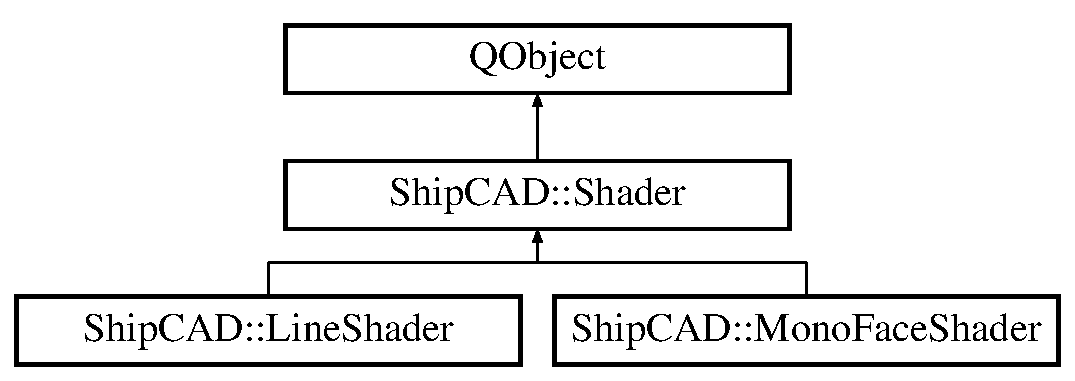
\includegraphics[height=3.950617cm]{classShipCAD_1_1Shader}
\end{center}
\end{figure}
\subsection*{Public Member Functions}
\begin{DoxyCompactItemize}
\item 
\hyperlink{classShipCAD_1_1Shader_a36bc24054e22fb965b04dae9a2b76eb7}{Shader} (\hyperlink{classShipCAD_1_1Viewport}{Viewport} $\ast$vp)
\item 
virtual \hyperlink{classShipCAD_1_1Shader_aff01df87e8a102f270b5b135a295e59d}{$\sim$\-Shader} ()
\item 
virtual void \hyperlink{classShipCAD_1_1Shader_a011fae279e362f548e8c4e4b35b7291e}{initialize} (const char $\ast$vertex\-Shader\-Source, const char $\ast$fragment\-Shader\-Source, std\-::vector$<$ std\-::string $>$ uniforms, std\-::vector$<$ std\-::string $>$ attributes)
\item 
void \hyperlink{classShipCAD_1_1Shader_ac8faec958f9d5806510d39be5f512c8e}{add\-Uniform} (const std\-::string \&name)
\item 
void \hyperlink{classShipCAD_1_1Shader_a6a298be357d7860d859aedbe397b81b9}{add\-Attribute} (const std\-::string \&name)
\item 
void \hyperlink{classShipCAD_1_1Shader_a7d7fe16e4eb06ad1eb19e22b38cff96e}{set\-Matrix} (const Q\-Matrix4x4 \&matrix)
\item 
void \hyperlink{classShipCAD_1_1Shader_a00c06ead1e413d5d5ecbced82478f753}{bind} ()
\item 
void \hyperlink{classShipCAD_1_1Shader_a0f41d7628964320846101cf5938a928e}{release} ()
\end{DoxyCompactItemize}
\subsection*{Protected Attributes}
\begin{DoxyCompactItemize}
\item 
\hyperlink{classShipCAD_1_1Viewport}{Viewport} $\ast$ \hyperlink{classShipCAD_1_1Shader_a0ee19c28f4fd4260b70095ccd433d546}{\-\_\-viewport}
\item 
Q\-Open\-G\-L\-Shader\-Program $\ast$ \hyperlink{classShipCAD_1_1Shader_a3967404471db3284a2448c4a39b8c230}{\-\_\-program}
\item 
std\-::map$<$ std\-::string, G\-Luint $>$ \hyperlink{classShipCAD_1_1Shader_a5c98e4ae6e3403f179a3fcf204b34baf}{\-\_\-uniforms}
\item 
std\-::map$<$ std\-::string, G\-Luint $>$ \hyperlink{classShipCAD_1_1Shader_af2f710f7b4d792fea09ddd11ab0cdf25}{\-\_\-attributes}
\end{DoxyCompactItemize}


\subsection{Detailed Description}


Definition at line 45 of file shader.\-h.



\subsection{Constructor \& Destructor Documentation}
\hypertarget{classShipCAD_1_1Shader_a36bc24054e22fb965b04dae9a2b76eb7}{\index{Ship\-C\-A\-D\-::\-Shader@{Ship\-C\-A\-D\-::\-Shader}!Shader@{Shader}}
\index{Shader@{Shader}!ShipCAD::Shader@{Ship\-C\-A\-D\-::\-Shader}}
\subsubsection[{Shader}]{\setlength{\rightskip}{0pt plus 5cm}Shader\-::\-Shader (
\begin{DoxyParamCaption}
\item[{{\bf Viewport} $\ast$}]{vp}
\end{DoxyParamCaption}
)\hspace{0.3cm}{\ttfamily [explicit]}}}\label{classShipCAD_1_1Shader_a36bc24054e22fb965b04dae9a2b76eb7}


Definition at line 42 of file shader.\-cpp.

\hypertarget{classShipCAD_1_1Shader_aff01df87e8a102f270b5b135a295e59d}{\index{Ship\-C\-A\-D\-::\-Shader@{Ship\-C\-A\-D\-::\-Shader}!$\sim$\-Shader@{$\sim$\-Shader}}
\index{$\sim$\-Shader@{$\sim$\-Shader}!ShipCAD::Shader@{Ship\-C\-A\-D\-::\-Shader}}
\subsubsection[{$\sim$\-Shader}]{\setlength{\rightskip}{0pt plus 5cm}Shader\-::$\sim$\-Shader (
\begin{DoxyParamCaption}
{}
\end{DoxyParamCaption}
)\hspace{0.3cm}{\ttfamily [virtual]}}}\label{classShipCAD_1_1Shader_aff01df87e8a102f270b5b135a295e59d}


Definition at line 48 of file shader.\-cpp.



\subsection{Member Function Documentation}
\hypertarget{classShipCAD_1_1Shader_a6a298be357d7860d859aedbe397b81b9}{\index{Ship\-C\-A\-D\-::\-Shader@{Ship\-C\-A\-D\-::\-Shader}!add\-Attribute@{add\-Attribute}}
\index{add\-Attribute@{add\-Attribute}!ShipCAD::Shader@{Ship\-C\-A\-D\-::\-Shader}}
\subsubsection[{add\-Attribute}]{\setlength{\rightskip}{0pt plus 5cm}void Shader\-::add\-Attribute (
\begin{DoxyParamCaption}
\item[{const std\-::string \&}]{name}
\end{DoxyParamCaption}
)}}\label{classShipCAD_1_1Shader_a6a298be357d7860d859aedbe397b81b9}


Definition at line 79 of file shader.\-cpp.

\hypertarget{classShipCAD_1_1Shader_ac8faec958f9d5806510d39be5f512c8e}{\index{Ship\-C\-A\-D\-::\-Shader@{Ship\-C\-A\-D\-::\-Shader}!add\-Uniform@{add\-Uniform}}
\index{add\-Uniform@{add\-Uniform}!ShipCAD::Shader@{Ship\-C\-A\-D\-::\-Shader}}
\subsubsection[{add\-Uniform}]{\setlength{\rightskip}{0pt plus 5cm}void Shader\-::add\-Uniform (
\begin{DoxyParamCaption}
\item[{const std\-::string \&}]{name}
\end{DoxyParamCaption}
)}}\label{classShipCAD_1_1Shader_ac8faec958f9d5806510d39be5f512c8e}


Definition at line 72 of file shader.\-cpp.

\hypertarget{classShipCAD_1_1Shader_a00c06ead1e413d5d5ecbced82478f753}{\index{Ship\-C\-A\-D\-::\-Shader@{Ship\-C\-A\-D\-::\-Shader}!bind@{bind}}
\index{bind@{bind}!ShipCAD::Shader@{Ship\-C\-A\-D\-::\-Shader}}
\subsubsection[{bind}]{\setlength{\rightskip}{0pt plus 5cm}void Ship\-C\-A\-D\-::\-Shader\-::bind (
\begin{DoxyParamCaption}
{}
\end{DoxyParamCaption}
)\hspace{0.3cm}{\ttfamily [inline]}}}\label{classShipCAD_1_1Shader_a00c06ead1e413d5d5ecbced82478f753}


Definition at line 64 of file shader.\-h.

\hypertarget{classShipCAD_1_1Shader_a011fae279e362f548e8c4e4b35b7291e}{\index{Ship\-C\-A\-D\-::\-Shader@{Ship\-C\-A\-D\-::\-Shader}!initialize@{initialize}}
\index{initialize@{initialize}!ShipCAD::Shader@{Ship\-C\-A\-D\-::\-Shader}}
\subsubsection[{initialize}]{\setlength{\rightskip}{0pt plus 5cm}void Shader\-::initialize (
\begin{DoxyParamCaption}
\item[{const char $\ast$}]{vertex\-Shader\-Source, }
\item[{const char $\ast$}]{fragment\-Shader\-Source, }
\item[{std\-::vector$<$ std\-::string $>$}]{uniforms, }
\item[{std\-::vector$<$ std\-::string $>$}]{attributes}
\end{DoxyParamCaption}
)\hspace{0.3cm}{\ttfamily [virtual]}}}\label{classShipCAD_1_1Shader_a011fae279e362f548e8c4e4b35b7291e}


Definition at line 53 of file shader.\-cpp.

\hypertarget{classShipCAD_1_1Shader_a0f41d7628964320846101cf5938a928e}{\index{Ship\-C\-A\-D\-::\-Shader@{Ship\-C\-A\-D\-::\-Shader}!release@{release}}
\index{release@{release}!ShipCAD::Shader@{Ship\-C\-A\-D\-::\-Shader}}
\subsubsection[{release}]{\setlength{\rightskip}{0pt plus 5cm}void Ship\-C\-A\-D\-::\-Shader\-::release (
\begin{DoxyParamCaption}
{}
\end{DoxyParamCaption}
)\hspace{0.3cm}{\ttfamily [inline]}}}\label{classShipCAD_1_1Shader_a0f41d7628964320846101cf5938a928e}


Definition at line 65 of file shader.\-h.

\hypertarget{classShipCAD_1_1Shader_a7d7fe16e4eb06ad1eb19e22b38cff96e}{\index{Ship\-C\-A\-D\-::\-Shader@{Ship\-C\-A\-D\-::\-Shader}!set\-Matrix@{set\-Matrix}}
\index{set\-Matrix@{set\-Matrix}!ShipCAD::Shader@{Ship\-C\-A\-D\-::\-Shader}}
\subsubsection[{set\-Matrix}]{\setlength{\rightskip}{0pt plus 5cm}void Shader\-::set\-Matrix (
\begin{DoxyParamCaption}
\item[{const Q\-Matrix4x4 \&}]{matrix}
\end{DoxyParamCaption}
)}}\label{classShipCAD_1_1Shader_a7d7fe16e4eb06ad1eb19e22b38cff96e}


Definition at line 86 of file shader.\-cpp.



\subsection{Member Data Documentation}
\hypertarget{classShipCAD_1_1Shader_af2f710f7b4d792fea09ddd11ab0cdf25}{\index{Ship\-C\-A\-D\-::\-Shader@{Ship\-C\-A\-D\-::\-Shader}!\-\_\-attributes@{\-\_\-attributes}}
\index{\-\_\-attributes@{\-\_\-attributes}!ShipCAD::Shader@{Ship\-C\-A\-D\-::\-Shader}}
\subsubsection[{\-\_\-attributes}]{\setlength{\rightskip}{0pt plus 5cm}std\-::map$<$std\-::string, G\-Luint$>$ Ship\-C\-A\-D\-::\-Shader\-::\-\_\-attributes\hspace{0.3cm}{\ttfamily [protected]}}}\label{classShipCAD_1_1Shader_af2f710f7b4d792fea09ddd11ab0cdf25}


Definition at line 72 of file shader.\-h.

\hypertarget{classShipCAD_1_1Shader_a3967404471db3284a2448c4a39b8c230}{\index{Ship\-C\-A\-D\-::\-Shader@{Ship\-C\-A\-D\-::\-Shader}!\-\_\-program@{\-\_\-program}}
\index{\-\_\-program@{\-\_\-program}!ShipCAD::Shader@{Ship\-C\-A\-D\-::\-Shader}}
\subsubsection[{\-\_\-program}]{\setlength{\rightskip}{0pt plus 5cm}Q\-Open\-G\-L\-Shader\-Program$\ast$ Ship\-C\-A\-D\-::\-Shader\-::\-\_\-program\hspace{0.3cm}{\ttfamily [protected]}}}\label{classShipCAD_1_1Shader_a3967404471db3284a2448c4a39b8c230}


Definition at line 70 of file shader.\-h.

\hypertarget{classShipCAD_1_1Shader_a5c98e4ae6e3403f179a3fcf204b34baf}{\index{Ship\-C\-A\-D\-::\-Shader@{Ship\-C\-A\-D\-::\-Shader}!\-\_\-uniforms@{\-\_\-uniforms}}
\index{\-\_\-uniforms@{\-\_\-uniforms}!ShipCAD::Shader@{Ship\-C\-A\-D\-::\-Shader}}
\subsubsection[{\-\_\-uniforms}]{\setlength{\rightskip}{0pt plus 5cm}std\-::map$<$std\-::string, G\-Luint$>$ Ship\-C\-A\-D\-::\-Shader\-::\-\_\-uniforms\hspace{0.3cm}{\ttfamily [protected]}}}\label{classShipCAD_1_1Shader_a5c98e4ae6e3403f179a3fcf204b34baf}


Definition at line 71 of file shader.\-h.

\hypertarget{classShipCAD_1_1Shader_a0ee19c28f4fd4260b70095ccd433d546}{\index{Ship\-C\-A\-D\-::\-Shader@{Ship\-C\-A\-D\-::\-Shader}!\-\_\-viewport@{\-\_\-viewport}}
\index{\-\_\-viewport@{\-\_\-viewport}!ShipCAD::Shader@{Ship\-C\-A\-D\-::\-Shader}}
\subsubsection[{\-\_\-viewport}]{\setlength{\rightskip}{0pt plus 5cm}{\bf Viewport}$\ast$ Ship\-C\-A\-D\-::\-Shader\-::\-\_\-viewport\hspace{0.3cm}{\ttfamily [protected]}}}\label{classShipCAD_1_1Shader_a0ee19c28f4fd4260b70095ccd433d546}


Definition at line 69 of file shader.\-h.



The documentation for this class was generated from the following files\-:\begin{DoxyCompactItemize}
\item 
Ship\-C\-A\-Dlib/\hyperlink{shader_8h}{shader.\-h}\item 
Ship\-C\-A\-Dlib/\hyperlink{shader_8cpp}{shader.\-cpp}\end{DoxyCompactItemize}

\hypertarget{classShipCAD_1_1ShipCADModel}{\section{Ship\-C\-A\-D\-:\-:Ship\-C\-A\-D\-Model Class Reference}
\label{classShipCAD_1_1ShipCADModel}\index{Ship\-C\-A\-D\-::\-Ship\-C\-A\-D\-Model@{Ship\-C\-A\-D\-::\-Ship\-C\-A\-D\-Model}}
}


{\ttfamily \#include $<$shipcadmodel.\-h$>$}

Inheritance diagram for Ship\-C\-A\-D\-:\-:Ship\-C\-A\-D\-Model\-:\begin{figure}[H]
\begin{center}
\leavevmode
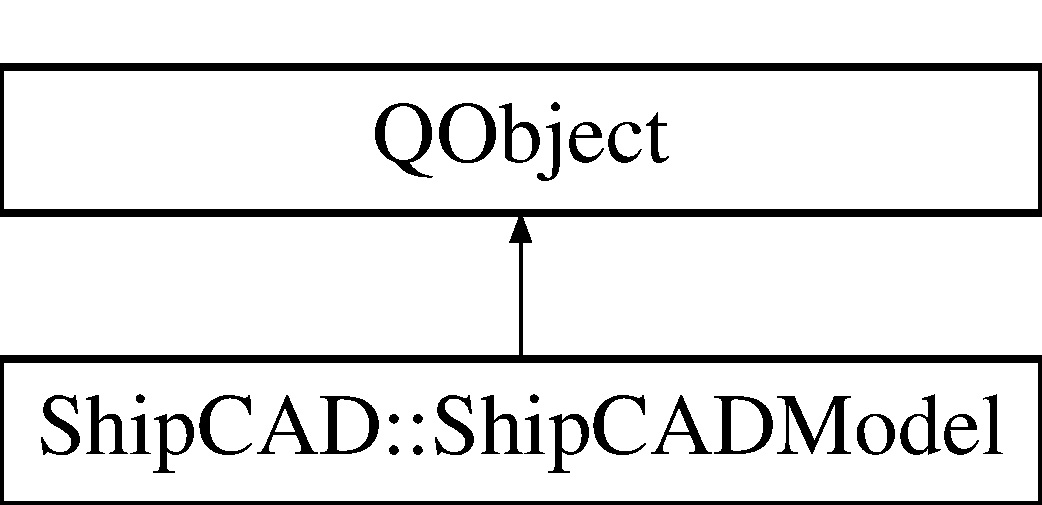
\includegraphics[height=2.000000cm]{classShipCAD_1_1ShipCADModel}
\end{center}
\end{figure}
\subsection*{Signals}
\begin{DoxyCompactItemize}
\item 
void \hyperlink{classShipCAD_1_1ShipCADModel_ab1aed79b8aa1de37e47b73895d0109a2}{on\-File\-Changed} ()
\item 
void \hyperlink{classShipCAD_1_1ShipCADModel_a6220a9a190b01f64ff47fedc55bdf8f4}{on\-Change\-Cursor\-Increment} ()
\item 
void \hyperlink{classShipCAD_1_1ShipCADModel_a182524b67e4bd1fcfbf87a23dd9e2002}{on\-Update\-Geometry\-Info} ()
\item 
void \hyperlink{classShipCAD_1_1ShipCADModel_adaa7b692532a8e09fbb06d24979882f3}{on\-Update\-Visibility\-Info} ()
\item 
void \hyperlink{classShipCAD_1_1ShipCADModel_a7becf2a008e66bdac7f77c8c7026c713}{changed\-Layer\-Data} ()
\item 
void \hyperlink{classShipCAD_1_1ShipCADModel_a8aee085180cb37bf822fb856a270a3b3}{change\-Active\-Layer} ()
\end{DoxyCompactItemize}
\subsection*{Public Member Functions}
\begin{DoxyCompactItemize}
\item 
\hyperlink{classShipCAD_1_1ShipCADModel_abede72e53058c2ecf8dc2c4b2a7c8014}{Ship\-C\-A\-D\-Model} ()
\item 
\hyperlink{classShipCAD_1_1ShipCADModel_a69faa69f492a5aad941990319e5e88c0}{$\sim$\-Ship\-C\-A\-D\-Model} ()
\item 
\hyperlink{classShipCAD_1_1Visibility}{Visibility} \& \hyperlink{classShipCAD_1_1ShipCADModel_a50cca4c783baeba58c8068c9b8a5d6a4}{get\-Visibility} ()
\item 
\hyperlink{classShipCAD_1_1ProjectSettings}{Project\-Settings} \& \hyperlink{classShipCAD_1_1ShipCADModel_a94a8eed8ac8ff4ad8287a0a1113e3271}{get\-Project\-Settings} ()
\item 
\hyperlink{classShipCAD_1_1Preferences}{Preferences} \& \hyperlink{classShipCAD_1_1ShipCADModel_aa6af8872deba5b401ac575a85901a265}{get\-Preferences} ()
\item 
void \hyperlink{classShipCAD_1_1ShipCADModel_abefac47aa19318b4ae3c82108dfe4585}{build\-Valid\-Frame\-Table} (bool close\-\_\-at\-\_\-deck)
\begin{DoxyCompactList}\small\item\em Assembles all stations and builds a 2\-D bodyplan. \end{DoxyCompactList}\item 
bool \hyperlink{classShipCAD_1_1ShipCADModel_a0c7a15b80b5013066fd77f46e57850ef}{is\-Build} ()
\item 
void \hyperlink{classShipCAD_1_1ShipCADModel_ab221977f2a8bd4d51d6ee777be0d7b8a}{set\-Build} (bool set)
\item 
\hyperlink{classShipCAD_1_1SubdivisionControlPoint}{Subdivision\-Control\-Point} $\ast$ \hyperlink{classShipCAD_1_1ShipCADModel_afe13cf557e067ae883433aa6f5afaf6a}{get\-Active\-Control\-Point} () const 
\begin{DoxyCompactList}\small\item\em get the active control point \end{DoxyCompactList}\item 
void \hyperlink{classShipCAD_1_1ShipCADModel_a523a7e9948d95a71e9008d386daeafee}{set\-Active\-Control\-Point} (\hyperlink{classShipCAD_1_1SubdivisionControlPoint}{Subdivision\-Control\-Point} $\ast$pt)
\begin{DoxyCompactList}\small\item\em set the active control point \end{DoxyCompactList}\item 
\hyperlink{namespaceShipCAD_ae13c7e36dfb1e2300741a631041cd915}{precision\-\_\-t} \hyperlink{classShipCAD_1_1ShipCADModel_a949318726227fe0ba274b34d2ea4528a}{get\-Precision} ()
\begin{DoxyCompactList}\small\item\em get precision of model \end{DoxyCompactList}\item 
void \hyperlink{classShipCAD_1_1ShipCADModel_a6133fe12cd13b6ce24424e19a8b1e433}{set\-Precision} (\hyperlink{namespaceShipCAD_ae13c7e36dfb1e2300741a631041cd915}{precision\-\_\-t} precision)
\begin{DoxyCompactList}\small\item\em set precision of model \end{DoxyCompactList}\item 
\hyperlink{namespaceShipCAD_af3a6fa23a7318acbda7b0066b53d694f}{version\-\_\-t} \hyperlink{classShipCAD_1_1ShipCADModel_a17ecfdd29efc03ed2580b89f5da955c8}{get\-File\-Version} ()
\item 
void \hyperlink{classShipCAD_1_1ShipCADModel_a44ac7a48c0c01cae73bf723120071e72}{set\-File\-Version} (\hyperlink{namespaceShipCAD_af3a6fa23a7318acbda7b0066b53d694f}{version\-\_\-t} v)
\item 
\hyperlink{namespaceShipCAD_a9910f0963197f9df6125398efd4fa139}{Intersection\-Vector} \& \hyperlink{classShipCAD_1_1ShipCADModel_a86da3ca66e90403ead21ccc67f584c52}{get\-Stations} ()
\item 
\hyperlink{namespaceShipCAD_a9910f0963197f9df6125398efd4fa139}{Intersection\-Vector} \& \hyperlink{classShipCAD_1_1ShipCADModel_a6c147a75fa02e43145de346efb9542fd}{get\-Waterlines} ()
\item 
\hyperlink{namespaceShipCAD_a9910f0963197f9df6125398efd4fa139}{Intersection\-Vector} \& \hyperlink{classShipCAD_1_1ShipCADModel_a8908d7adff0b1aa1ed118103c02c5402}{get\-Buttocks} ()
\item 
\hyperlink{namespaceShipCAD_a9910f0963197f9df6125398efd4fa139}{Intersection\-Vector} \& \hyperlink{classShipCAD_1_1ShipCADModel_a19864f7628c596553f7c89247715b10a}{get\-Diagonals} ()
\item 
\hyperlink{namespaceShipCAD_aa9dd7a826ae5254e377dac43ea19da80}{Subdivision\-Control\-Curve\-Vector} \& \hyperlink{classShipCAD_1_1ShipCADModel_ac631aaf60a936bb5b22bcab59cb7d6a4}{get\-Control\-Curves} ()
\item 
\hyperlink{classShipCAD_1_1Flowline}{Flowline} $\ast$ \hyperlink{classShipCAD_1_1ShipCADModel_afc5654f671a17dd6672230648842975e}{get\-Flowline} (size\-\_\-t index)
\item 
\hyperlink{namespaceShipCAD_a66144e3f3a53da01f51c9bdb94fcae31}{edit\-\_\-mode\-\_\-t} \hyperlink{classShipCAD_1_1ShipCADModel_a355525c21cd0a9a4a88846b5587a236c}{get\-Edit\-Mode} ()
\item 
void \hyperlink{classShipCAD_1_1ShipCADModel_a2636160d900b8d8b00802ae78ee87925}{set\-Edit\-Mode} (\hyperlink{namespaceShipCAD_a66144e3f3a53da01f51c9bdb94fcae31}{edit\-\_\-mode\-\_\-t} mode)
\item 
size\-\_\-t \hyperlink{classShipCAD_1_1ShipCADModel_ac01e316c15b67f35e5db96aa186d362e}{count\-Selected\-Items} ()
\begin{DoxyCompactList}\small\item\em count the number of currently selected items \end{DoxyCompactList}\item 
void \hyperlink{classShipCAD_1_1ShipCADModel_a690bd5621d82d15a28ea59c09ded99d8}{clear\-Selected\-Items} ()
\begin{DoxyCompactList}\small\item\em clear all selected items \end{DoxyCompactList}\item 
Q\-String \hyperlink{classShipCAD_1_1ShipCADModel_a7cdd359f050f81975d1992a7d161ce87}{get\-Filename} ()
\begin{DoxyCompactList}\small\item\em name of file \end{DoxyCompactList}\item 
void \hyperlink{classShipCAD_1_1ShipCADModel_a07daf75d876f80296f841f5c8d2327cb}{set\-Filename} (const Q\-String \&name)
\begin{DoxyCompactList}\small\item\em set the name of the file \end{DoxyCompactList}\item 
bool \hyperlink{classShipCAD_1_1ShipCADModel_af63013461d2ef6ee7221d72a42949d7c}{is\-Filename\-Set} ()
\begin{DoxyCompactList}\small\item\em get flag for filename set \end{DoxyCompactList}\item 
void \hyperlink{classShipCAD_1_1ShipCADModel_a960f3e97ef2aa847c9bb7cdc7731cd39}{set\-Filename\-Set} (bool flag)
\begin{DoxyCompactList}\small\item\em set flag for filename set \end{DoxyCompactList}\item 
\hyperlink{namespaceShipCAD_a0c7b012d8868cbb43871cf0bf303ccc6}{Hydrostatic\-Calc\-Vector} \& \hyperlink{classShipCAD_1_1ShipCADModel_aafc30dd7d6b9db4ccfc7bf1c4e2b3b11}{get\-Hydrostatic\-Calculations} ()
\item 
\hyperlink{classShipCAD_1_1SubdivisionLayer}{Subdivision\-Layer} $\ast$ \hyperlink{classShipCAD_1_1ShipCADModel_a5aa1e9aa14350f2e0980112a81613ca6}{get\-Active\-Layer} ()
\item 
size\-\_\-t \hyperlink{classShipCAD_1_1ShipCADModel_afb23b08b1014fc176ff864b8f154a84b}{number\-Of\-Layers} ()
\item 
\hyperlink{classShipCAD_1_1SubdivisionLayer}{Subdivision\-Layer} $\ast$ \hyperlink{classShipCAD_1_1ShipCADModel_ae13e425deb59f7b4f0c95cc02230f097}{get\-Layer} (size\-\_\-t index)
\item 
size\-\_\-t \hyperlink{classShipCAD_1_1ShipCADModel_afdb9bccb1cf9e3bf8aa853d81ff11d39}{number\-Of\-Flowlines} ()
\item 
size\-\_\-t \hyperlink{classShipCAD_1_1ShipCADModel_afb8cc5aaf19a6c1c687550fd9de1739e}{number\-Of\-Locked\-Points} ()
\item 
size\-\_\-t \hyperlink{classShipCAD_1_1ShipCADModel_a099d0530e99261318f6332220a331010}{number\-Of\-Viewports} ()
\item 
bool \hyperlink{classShipCAD_1_1ShipCADModel_ada688a626562a513c03f0a19c6233eae}{is\-Selected\-Marker} (\hyperlink{classShipCAD_1_1Marker}{Marker} $\ast$mark)
\item 
void \hyperlink{classShipCAD_1_1ShipCADModel_afd7e984f4070d08cb16264c1b731580f}{set\-Selected\-Marker} (\hyperlink{classShipCAD_1_1Marker}{Marker} $\ast$mark)
\item 
void \hyperlink{classShipCAD_1_1ShipCADModel_a7fb06b0a1fa75ef02597752fc3f691a2}{remove\-Selected\-Marker} (\hyperlink{classShipCAD_1_1Marker}{Marker} $\ast$mark)
\item 
bool \hyperlink{classShipCAD_1_1ShipCADModel_a64493dfc69513b4d9425e3736e41b596}{adjust\-Markers} ()
\item 
bool \hyperlink{classShipCAD_1_1ShipCADModel_a9276e43cb3f7917782f91a7cf3faa215}{is\-Selected\-Flowline} (const \hyperlink{classShipCAD_1_1Flowline}{Flowline} $\ast$flow) const 
\begin{DoxyCompactList}\small\item\em is the flowline selected \end{DoxyCompactList}\item 
void \hyperlink{classShipCAD_1_1ShipCADModel_af61065a1e9050cff7cb91c8312082e2a}{set\-Selected\-Flowline} (const \hyperlink{classShipCAD_1_1Flowline}{Flowline} $\ast$flow)
\begin{DoxyCompactList}\small\item\em set a flowline as selected \end{DoxyCompactList}\item 
void \hyperlink{classShipCAD_1_1ShipCADModel_ad16bba5c648dec8cddfe23ed9b07615a}{remove\-Selected\-Flowline} (const \hyperlink{classShipCAD_1_1Flowline}{Flowline} $\ast$flow)
\begin{DoxyCompactList}\small\item\em deselect a flowline \end{DoxyCompactList}\item 
void \hyperlink{classShipCAD_1_1ShipCADModel_a6d868bbb71f72c46e6827adeed8afc4b}{add\-Viewport} (\hyperlink{classShipCAD_1_1Viewport}{Viewport} $\ast$vp)
\item 
\hyperlink{classShipCAD_1_1SubdivisionSurface}{Subdivision\-Surface} $\ast$ \hyperlink{classShipCAD_1_1ShipCADModel_a6941ad7a2b167419e844823fa8461019}{get\-Surface} ()
\item 
bool \hyperlink{classShipCAD_1_1ShipCADModel_a2cf41d2e7463763c81c7850fe953437e}{is\-File\-Changed} ()
\begin{DoxyCompactList}\small\item\em file changed flag \end{DoxyCompactList}\item 
void \hyperlink{classShipCAD_1_1ShipCADModel_a98ebcb64c5c759cbd0ae6e817b7168b2}{set\-File\-Changed} (bool changed)
\begin{DoxyCompactList}\small\item\em set file changed flag \end{DoxyCompactList}\item 
void \hyperlink{classShipCAD_1_1ShipCADModel_ab79232c9ce03bda04f47ff614f87cea4}{add\-Undo\-Object} (\hyperlink{classShipCAD_1_1UndoObject}{Undo\-Object} $\ast$newundo)
\begin{DoxyCompactList}\small\item\em add undo object \end{DoxyCompactList}\item 
\hyperlink{classShipCAD_1_1UndoObject}{Undo\-Object} $\ast$ \hyperlink{classShipCAD_1_1ShipCADModel_a0acb4ae206e2caee0f87ebd229b7c90b}{get\-Undo\-Object} (size\-\_\-t index)
\begin{DoxyCompactList}\small\item\em get undo object at index \end{DoxyCompactList}\item 
void \hyperlink{classShipCAD_1_1ShipCADModel_a0c14ab36acacc74411446a65ffadaa06}{delete\-Undo\-Object} (\hyperlink{classShipCAD_1_1UndoObject}{Undo\-Object} $\ast$deleted)
\begin{DoxyCompactList}\small\item\em get undo object at index \end{DoxyCompactList}\item 
size\-\_\-t \hyperlink{classShipCAD_1_1ShipCADModel_a1d7ffa7d873dc1f43d21a62054ae356c}{undo\-Count} ()
\begin{DoxyCompactList}\small\item\em number of undo objects \end{DoxyCompactList}\item 
size\-\_\-t \hyperlink{classShipCAD_1_1ShipCADModel_a28d6c179e54a1e19997a0da2a38e4ca5}{undo\-Position} ()
\begin{DoxyCompactList}\small\item\em current undo index position \end{DoxyCompactList}\item 
size\-\_\-t \hyperlink{classShipCAD_1_1ShipCADModel_a5d2116df534ab1347961c6ab9748d1f1}{prev\-Undo\-Position} ()
\begin{DoxyCompactList}\small\item\em previous undo index position \end{DoxyCompactList}\item 
void \hyperlink{classShipCAD_1_1ShipCADModel_aa466832784532e736a1c2a16681a6d04}{set\-Undo\-Position} (size\-\_\-t index)
\begin{DoxyCompactList}\small\item\em set undo index position \end{DoxyCompactList}\item 
void \hyperlink{classShipCAD_1_1ShipCADModel_a27acd2ab4c6486a23db0b054962381bd}{set\-Prev\-Undo\-Position} (size\-\_\-t index)
\begin{DoxyCompactList}\small\item\em set previous undo index position \end{DoxyCompactList}\item 
size\-\_\-t \hyperlink{classShipCAD_1_1ShipCADModel_a0ab3edfdc89a6e297343d7c31b21658c}{get\-Undo\-Memory} ()
\begin{DoxyCompactList}\small\item\em get amount of memory used for undo \end{DoxyCompactList}\item 
void \hyperlink{classShipCAD_1_1ShipCADModel_af06c21c121f42e1ac4e5510d8c9ed3cd}{redraw} ()
\begin{DoxyCompactList}\small\item\em redraw the model \end{DoxyCompactList}\item 
float \hyperlink{classShipCAD_1_1ShipCADModel_a8cde3b7ca816132af3c722cd31af3107}{find\-Lowest\-Hydrostatics\-Point} ()
\begin{DoxyCompactList}\small\item\em get the lowest underwater point of hull \end{DoxyCompactList}\item 
void \hyperlink{classShipCAD_1_1ShipCADModel_ad3e49bc04c73dc221e48d15974b68f41}{load\-Binary} (\hyperlink{classShipCAD_1_1FileBuffer}{File\-Buffer} \&source)
\item 
void \hyperlink{classShipCAD_1_1ShipCADModel_a64c7c4ddffffdd1be2f27eb4210af2b7}{save\-Binary} (\hyperlink{classShipCAD_1_1FileBuffer}{File\-Buffer} \&dest)
\item 
void \hyperlink{classShipCAD_1_1ShipCADModel_a0d8f9cb2ce8038f6e65d90e8cab275e7}{save\-Part} (std\-::vector$<$ \hyperlink{classShipCAD_1_1SubdivisionFace}{Subdivision\-Face} $\ast$ $>$ faces)
\item 
void \hyperlink{classShipCAD_1_1ShipCADModel_a2e03bcc700adfcf768e257c91f5b0df9}{rebuild\-Model} ()
\item 
void \hyperlink{classShipCAD_1_1ShipCADModel_abf593b803e96a1fd8e56f36b3b6d0954}{draw} (\hyperlink{classShipCAD_1_1Viewport}{Viewport} \&vp)
\item 
void \hyperlink{classShipCAD_1_1ShipCADModel_ad2f9dfd32667e9ac690de184b7e576f1}{clear} ()
\item 
void \hyperlink{classShipCAD_1_1ShipCADModel_a9d693b6b2180ce94e88224df49b909a2}{clear\-Undo} ()
\item 
void \hyperlink{classShipCAD_1_1ShipCADModel_a7ab84a738b747c4fcb2c3627e56d4bd0}{extents} (Q\-Vector3\-D \&min, Q\-Vector3\-D \&max)
\begin{DoxyCompactList}\small\item\em find the bounding box of the model \end{DoxyCompactList}\end{DoxyCompactItemize}
\subsection*{Protected Member Functions}
\begin{DoxyCompactItemize}
\item 
void \hyperlink{classShipCAD_1_1ShipCADModel_a04d6e146dff42232658531c64d064217}{draw\-Grid} (\hyperlink{classShipCAD_1_1Viewport}{Viewport} \&vp, \hyperlink{classShipCAD_1_1LineShader}{Line\-Shader} $\ast$lineshader)
\end{DoxyCompactItemize}


\subsection{Detailed Description}


Definition at line 62 of file shipcadmodel.\-h.



\subsection{Constructor \& Destructor Documentation}
\hypertarget{classShipCAD_1_1ShipCADModel_abede72e53058c2ecf8dc2c4b2a7c8014}{\index{Ship\-C\-A\-D\-::\-Ship\-C\-A\-D\-Model@{Ship\-C\-A\-D\-::\-Ship\-C\-A\-D\-Model}!Ship\-C\-A\-D\-Model@{Ship\-C\-A\-D\-Model}}
\index{Ship\-C\-A\-D\-Model@{Ship\-C\-A\-D\-Model}!ShipCAD::ShipCADModel@{Ship\-C\-A\-D\-::\-Ship\-C\-A\-D\-Model}}
\subsubsection[{Ship\-C\-A\-D\-Model}]{\setlength{\rightskip}{0pt plus 5cm}Ship\-C\-A\-D\-Model\-::\-Ship\-C\-A\-D\-Model (
\begin{DoxyParamCaption}
{}
\end{DoxyParamCaption}
)\hspace{0.3cm}{\ttfamily [explicit]}}}\label{classShipCAD_1_1ShipCADModel_abede72e53058c2ecf8dc2c4b2a7c8014}


Definition at line 45 of file shipcadmodel.\-cpp.

\hypertarget{classShipCAD_1_1ShipCADModel_a69faa69f492a5aad941990319e5e88c0}{\index{Ship\-C\-A\-D\-::\-Ship\-C\-A\-D\-Model@{Ship\-C\-A\-D\-::\-Ship\-C\-A\-D\-Model}!$\sim$\-Ship\-C\-A\-D\-Model@{$\sim$\-Ship\-C\-A\-D\-Model}}
\index{$\sim$\-Ship\-C\-A\-D\-Model@{$\sim$\-Ship\-C\-A\-D\-Model}!ShipCAD::ShipCADModel@{Ship\-C\-A\-D\-::\-Ship\-C\-A\-D\-Model}}
\subsubsection[{$\sim$\-Ship\-C\-A\-D\-Model}]{\setlength{\rightskip}{0pt plus 5cm}Ship\-C\-A\-D\-Model\-::$\sim$\-Ship\-C\-A\-D\-Model (
\begin{DoxyParamCaption}
{}
\end{DoxyParamCaption}
)}}\label{classShipCAD_1_1ShipCADModel_a69faa69f492a5aad941990319e5e88c0}


Definition at line 60 of file shipcadmodel.\-cpp.



\subsection{Member Function Documentation}
\hypertarget{classShipCAD_1_1ShipCADModel_ab79232c9ce03bda04f47ff614f87cea4}{\index{Ship\-C\-A\-D\-::\-Ship\-C\-A\-D\-Model@{Ship\-C\-A\-D\-::\-Ship\-C\-A\-D\-Model}!add\-Undo\-Object@{add\-Undo\-Object}}
\index{add\-Undo\-Object@{add\-Undo\-Object}!ShipCAD::ShipCADModel@{Ship\-C\-A\-D\-::\-Ship\-C\-A\-D\-Model}}
\subsubsection[{add\-Undo\-Object}]{\setlength{\rightskip}{0pt plus 5cm}void Ship\-C\-A\-D\-Model\-::add\-Undo\-Object (
\begin{DoxyParamCaption}
\item[{{\bf Undo\-Object} $\ast$}]{newundo}
\end{DoxyParamCaption}
)}}\label{classShipCAD_1_1ShipCADModel_ab79232c9ce03bda04f47ff614f87cea4}


add undo object 


\begin{DoxyParams}{Parameters}
{\em new} & undo object \\
\hline
\end{DoxyParams}


Definition at line 223 of file shipcadmodel.\-cpp.

\hypertarget{classShipCAD_1_1ShipCADModel_a6d868bbb71f72c46e6827adeed8afc4b}{\index{Ship\-C\-A\-D\-::\-Ship\-C\-A\-D\-Model@{Ship\-C\-A\-D\-::\-Ship\-C\-A\-D\-Model}!add\-Viewport@{add\-Viewport}}
\index{add\-Viewport@{add\-Viewport}!ShipCAD::ShipCADModel@{Ship\-C\-A\-D\-::\-Ship\-C\-A\-D\-Model}}
\subsubsection[{add\-Viewport}]{\setlength{\rightskip}{0pt plus 5cm}void Ship\-C\-A\-D\-::\-Ship\-C\-A\-D\-Model\-::add\-Viewport (
\begin{DoxyParamCaption}
\item[{{\bf Viewport} $\ast$}]{vp}
\end{DoxyParamCaption}
)}}\label{classShipCAD_1_1ShipCADModel_a6d868bbb71f72c46e6827adeed8afc4b}
\hypertarget{classShipCAD_1_1ShipCADModel_a64493dfc69513b4d9425e3736e41b596}{\index{Ship\-C\-A\-D\-::\-Ship\-C\-A\-D\-Model@{Ship\-C\-A\-D\-::\-Ship\-C\-A\-D\-Model}!adjust\-Markers@{adjust\-Markers}}
\index{adjust\-Markers@{adjust\-Markers}!ShipCAD::ShipCADModel@{Ship\-C\-A\-D\-::\-Ship\-C\-A\-D\-Model}}
\subsubsection[{adjust\-Markers}]{\setlength{\rightskip}{0pt plus 5cm}bool Ship\-C\-A\-D\-Model\-::adjust\-Markers (
\begin{DoxyParamCaption}
{}
\end{DoxyParamCaption}
)}}\label{classShipCAD_1_1ShipCADModel_a64493dfc69513b4d9425e3736e41b596}


Definition at line 564 of file shipcadmodel.\-cpp.

\hypertarget{classShipCAD_1_1ShipCADModel_abefac47aa19318b4ae3c82108dfe4585}{\index{Ship\-C\-A\-D\-::\-Ship\-C\-A\-D\-Model@{Ship\-C\-A\-D\-::\-Ship\-C\-A\-D\-Model}!build\-Valid\-Frame\-Table@{build\-Valid\-Frame\-Table}}
\index{build\-Valid\-Frame\-Table@{build\-Valid\-Frame\-Table}!ShipCAD::ShipCADModel@{Ship\-C\-A\-D\-::\-Ship\-C\-A\-D\-Model}}
\subsubsection[{build\-Valid\-Frame\-Table}]{\setlength{\rightskip}{0pt plus 5cm}void Ship\-C\-A\-D\-Model\-::build\-Valid\-Frame\-Table (
\begin{DoxyParamCaption}
\item[{bool}]{close\-\_\-at\-\_\-deck}
\end{DoxyParamCaption}
)}}\label{classShipCAD_1_1ShipCADModel_abefac47aa19318b4ae3c82108dfe4585}


Assembles all stations and builds a 2\-D bodyplan. 


\begin{DoxyParams}{Parameters}
{\em close\-\_\-at\-\_\-deck} & \\
\hline
\end{DoxyParams}


Definition at line 101 of file shipcadmodel.\-cpp.

\hypertarget{classShipCAD_1_1ShipCADModel_a8aee085180cb37bf822fb856a270a3b3}{\index{Ship\-C\-A\-D\-::\-Ship\-C\-A\-D\-Model@{Ship\-C\-A\-D\-::\-Ship\-C\-A\-D\-Model}!change\-Active\-Layer@{change\-Active\-Layer}}
\index{change\-Active\-Layer@{change\-Active\-Layer}!ShipCAD::ShipCADModel@{Ship\-C\-A\-D\-::\-Ship\-C\-A\-D\-Model}}
\subsubsection[{change\-Active\-Layer}]{\setlength{\rightskip}{0pt plus 5cm}void Ship\-C\-A\-D\-::\-Ship\-C\-A\-D\-Model\-::change\-Active\-Layer (
\begin{DoxyParamCaption}
{}
\end{DoxyParamCaption}
)\hspace{0.3cm}{\ttfamily [signal]}}}\label{classShipCAD_1_1ShipCADModel_a8aee085180cb37bf822fb856a270a3b3}
\hypertarget{classShipCAD_1_1ShipCADModel_a7becf2a008e66bdac7f77c8c7026c713}{\index{Ship\-C\-A\-D\-::\-Ship\-C\-A\-D\-Model@{Ship\-C\-A\-D\-::\-Ship\-C\-A\-D\-Model}!changed\-Layer\-Data@{changed\-Layer\-Data}}
\index{changed\-Layer\-Data@{changed\-Layer\-Data}!ShipCAD::ShipCADModel@{Ship\-C\-A\-D\-::\-Ship\-C\-A\-D\-Model}}
\subsubsection[{changed\-Layer\-Data}]{\setlength{\rightskip}{0pt plus 5cm}void Ship\-C\-A\-D\-::\-Ship\-C\-A\-D\-Model\-::changed\-Layer\-Data (
\begin{DoxyParamCaption}
{}
\end{DoxyParamCaption}
)\hspace{0.3cm}{\ttfamily [signal]}}}\label{classShipCAD_1_1ShipCADModel_a7becf2a008e66bdac7f77c8c7026c713}
\hypertarget{classShipCAD_1_1ShipCADModel_ad2f9dfd32667e9ac690de184b7e576f1}{\index{Ship\-C\-A\-D\-::\-Ship\-C\-A\-D\-Model@{Ship\-C\-A\-D\-::\-Ship\-C\-A\-D\-Model}!clear@{clear}}
\index{clear@{clear}!ShipCAD::ShipCADModel@{Ship\-C\-A\-D\-::\-Ship\-C\-A\-D\-Model}}
\subsubsection[{clear}]{\setlength{\rightskip}{0pt plus 5cm}void Ship\-C\-A\-D\-Model\-::clear (
\begin{DoxyParamCaption}
{}
\end{DoxyParamCaption}
)}}\label{classShipCAD_1_1ShipCADModel_ad2f9dfd32667e9ac690de184b7e576f1}


Definition at line 65 of file shipcadmodel.\-cpp.

\hypertarget{classShipCAD_1_1ShipCADModel_a690bd5621d82d15a28ea59c09ded99d8}{\index{Ship\-C\-A\-D\-::\-Ship\-C\-A\-D\-Model@{Ship\-C\-A\-D\-::\-Ship\-C\-A\-D\-Model}!clear\-Selected\-Items@{clear\-Selected\-Items}}
\index{clear\-Selected\-Items@{clear\-Selected\-Items}!ShipCAD::ShipCADModel@{Ship\-C\-A\-D\-::\-Ship\-C\-A\-D\-Model}}
\subsubsection[{clear\-Selected\-Items}]{\setlength{\rightskip}{0pt plus 5cm}void Ship\-C\-A\-D\-Model\-::clear\-Selected\-Items (
\begin{DoxyParamCaption}
{}
\end{DoxyParamCaption}
)}}\label{classShipCAD_1_1ShipCADModel_a690bd5621d82d15a28ea59c09ded99d8}


clear all selected items 



Definition at line 201 of file shipcadmodel.\-cpp.

\hypertarget{classShipCAD_1_1ShipCADModel_a9d693b6b2180ce94e88224df49b909a2}{\index{Ship\-C\-A\-D\-::\-Ship\-C\-A\-D\-Model@{Ship\-C\-A\-D\-::\-Ship\-C\-A\-D\-Model}!clear\-Undo@{clear\-Undo}}
\index{clear\-Undo@{clear\-Undo}!ShipCAD::ShipCADModel@{Ship\-C\-A\-D\-::\-Ship\-C\-A\-D\-Model}}
\subsubsection[{clear\-Undo}]{\setlength{\rightskip}{0pt plus 5cm}void Ship\-C\-A\-D\-::\-Ship\-C\-A\-D\-Model\-::clear\-Undo (
\begin{DoxyParamCaption}
{}
\end{DoxyParamCaption}
)}}\label{classShipCAD_1_1ShipCADModel_a9d693b6b2180ce94e88224df49b909a2}
\hypertarget{classShipCAD_1_1ShipCADModel_ac01e316c15b67f35e5db96aa186d362e}{\index{Ship\-C\-A\-D\-::\-Ship\-C\-A\-D\-Model@{Ship\-C\-A\-D\-::\-Ship\-C\-A\-D\-Model}!count\-Selected\-Items@{count\-Selected\-Items}}
\index{count\-Selected\-Items@{count\-Selected\-Items}!ShipCAD::ShipCADModel@{Ship\-C\-A\-D\-::\-Ship\-C\-A\-D\-Model}}
\subsubsection[{count\-Selected\-Items}]{\setlength{\rightskip}{0pt plus 5cm}size\-\_\-t Ship\-C\-A\-D\-Model\-::count\-Selected\-Items (
\begin{DoxyParamCaption}
{}
\end{DoxyParamCaption}
)}}\label{classShipCAD_1_1ShipCADModel_ac01e316c15b67f35e5db96aa186d362e}


count the number of currently selected items 

\begin{DoxyReturn}{Returns}
number of selected items 
\end{DoxyReturn}


Definition at line 190 of file shipcadmodel.\-cpp.

\hypertarget{classShipCAD_1_1ShipCADModel_a0c14ab36acacc74411446a65ffadaa06}{\index{Ship\-C\-A\-D\-::\-Ship\-C\-A\-D\-Model@{Ship\-C\-A\-D\-::\-Ship\-C\-A\-D\-Model}!delete\-Undo\-Object@{delete\-Undo\-Object}}
\index{delete\-Undo\-Object@{delete\-Undo\-Object}!ShipCAD::ShipCADModel@{Ship\-C\-A\-D\-::\-Ship\-C\-A\-D\-Model}}
\subsubsection[{delete\-Undo\-Object}]{\setlength{\rightskip}{0pt plus 5cm}void Ship\-C\-A\-D\-Model\-::delete\-Undo\-Object (
\begin{DoxyParamCaption}
\item[{{\bf Undo\-Object} $\ast$}]{deleted}
\end{DoxyParamCaption}
)}}\label{classShipCAD_1_1ShipCADModel_a0c14ab36acacc74411446a65ffadaa06}


get undo object at index 


\begin{DoxyParams}{Parameters}
{\em index} & of undo object \\
\hline
\end{DoxyParams}
\begin{DoxyReturn}{Returns}
the undo object at index 
\end{DoxyReturn}

\begin{DoxyExceptions}{Exceptions}
{\em invalid\-\_\-argument} & \\
\hline
\end{DoxyExceptions}


Definition at line 235 of file shipcadmodel.\-cpp.

\hypertarget{classShipCAD_1_1ShipCADModel_abf593b803e96a1fd8e56f36b3b6d0954}{\index{Ship\-C\-A\-D\-::\-Ship\-C\-A\-D\-Model@{Ship\-C\-A\-D\-::\-Ship\-C\-A\-D\-Model}!draw@{draw}}
\index{draw@{draw}!ShipCAD::ShipCADModel@{Ship\-C\-A\-D\-::\-Ship\-C\-A\-D\-Model}}
\subsubsection[{draw}]{\setlength{\rightskip}{0pt plus 5cm}void Ship\-C\-A\-D\-Model\-::draw (
\begin{DoxyParamCaption}
\item[{{\bf Viewport} \&}]{vp}
\end{DoxyParamCaption}
)}}\label{classShipCAD_1_1ShipCADModel_abf593b803e96a1fd8e56f36b3b6d0954}


Definition at line 284 of file shipcadmodel.\-cpp.

\hypertarget{classShipCAD_1_1ShipCADModel_a04d6e146dff42232658531c64d064217}{\index{Ship\-C\-A\-D\-::\-Ship\-C\-A\-D\-Model@{Ship\-C\-A\-D\-::\-Ship\-C\-A\-D\-Model}!draw\-Grid@{draw\-Grid}}
\index{draw\-Grid@{draw\-Grid}!ShipCAD::ShipCADModel@{Ship\-C\-A\-D\-::\-Ship\-C\-A\-D\-Model}}
\subsubsection[{draw\-Grid}]{\setlength{\rightskip}{0pt plus 5cm}void Ship\-C\-A\-D\-Model\-::draw\-Grid (
\begin{DoxyParamCaption}
\item[{{\bf Viewport} \&}]{vp, }
\item[{{\bf Line\-Shader} $\ast$}]{lineshader}
\end{DoxyParamCaption}
)\hspace{0.3cm}{\ttfamily [protected]}}}\label{classShipCAD_1_1ShipCADModel_a04d6e146dff42232658531c64d064217}


Definition at line 266 of file shipcadmodel.\-cpp.

\hypertarget{classShipCAD_1_1ShipCADModel_a7ab84a738b747c4fcb2c3627e56d4bd0}{\index{Ship\-C\-A\-D\-::\-Ship\-C\-A\-D\-Model@{Ship\-C\-A\-D\-::\-Ship\-C\-A\-D\-Model}!extents@{extents}}
\index{extents@{extents}!ShipCAD::ShipCADModel@{Ship\-C\-A\-D\-::\-Ship\-C\-A\-D\-Model}}
\subsubsection[{extents}]{\setlength{\rightskip}{0pt plus 5cm}void Ship\-C\-A\-D\-Model\-::extents (
\begin{DoxyParamCaption}
\item[{Q\-Vector3\-D \&}]{min, }
\item[{Q\-Vector3\-D \&}]{max}
\end{DoxyParamCaption}
)}}\label{classShipCAD_1_1ShipCADModel_a7ab84a738b747c4fcb2c3627e56d4bd0}


find the bounding box of the model 


\begin{DoxyParams}{Parameters}
{\em the} & minimum corner of the bounding box \\
\hline
{\em the} & maximum corner of the bounding box \\
\hline
\end{DoxyParams}


Definition at line 106 of file shipcadmodel.\-cpp.

\hypertarget{classShipCAD_1_1ShipCADModel_a8cde3b7ca816132af3c722cd31af3107}{\index{Ship\-C\-A\-D\-::\-Ship\-C\-A\-D\-Model@{Ship\-C\-A\-D\-::\-Ship\-C\-A\-D\-Model}!find\-Lowest\-Hydrostatics\-Point@{find\-Lowest\-Hydrostatics\-Point}}
\index{find\-Lowest\-Hydrostatics\-Point@{find\-Lowest\-Hydrostatics\-Point}!ShipCAD::ShipCADModel@{Ship\-C\-A\-D\-::\-Ship\-C\-A\-D\-Model}}
\subsubsection[{find\-Lowest\-Hydrostatics\-Point}]{\setlength{\rightskip}{0pt plus 5cm}float Ship\-C\-A\-D\-Model\-::find\-Lowest\-Hydrostatics\-Point (
\begin{DoxyParamCaption}
{}
\end{DoxyParamCaption}
)}}\label{classShipCAD_1_1ShipCADModel_a8cde3b7ca816132af3c722cd31af3107}


get the lowest underwater point of hull 

\begin{DoxyReturn}{Returns}
lowest point of hull 
\end{DoxyReturn}


Definition at line 509 of file shipcadmodel.\-cpp.

\hypertarget{classShipCAD_1_1ShipCADModel_afe13cf557e067ae883433aa6f5afaf6a}{\index{Ship\-C\-A\-D\-::\-Ship\-C\-A\-D\-Model@{Ship\-C\-A\-D\-::\-Ship\-C\-A\-D\-Model}!get\-Active\-Control\-Point@{get\-Active\-Control\-Point}}
\index{get\-Active\-Control\-Point@{get\-Active\-Control\-Point}!ShipCAD::ShipCADModel@{Ship\-C\-A\-D\-::\-Ship\-C\-A\-D\-Model}}
\subsubsection[{get\-Active\-Control\-Point}]{\setlength{\rightskip}{0pt plus 5cm}{\bf Subdivision\-Control\-Point}$\ast$ Ship\-C\-A\-D\-::\-Ship\-C\-A\-D\-Model\-::get\-Active\-Control\-Point (
\begin{DoxyParamCaption}
{}
\end{DoxyParamCaption}
) const\hspace{0.3cm}{\ttfamily [inline]}}}\label{classShipCAD_1_1ShipCADModel_afe13cf557e067ae883433aa6f5afaf6a}


get the active control point 

\begin{DoxyReturn}{Returns}
the active control point or 0 
\end{DoxyReturn}


Definition at line 87 of file shipcadmodel.\-h.

\hypertarget{classShipCAD_1_1ShipCADModel_a5aa1e9aa14350f2e0980112a81613ca6}{\index{Ship\-C\-A\-D\-::\-Ship\-C\-A\-D\-Model@{Ship\-C\-A\-D\-::\-Ship\-C\-A\-D\-Model}!get\-Active\-Layer@{get\-Active\-Layer}}
\index{get\-Active\-Layer@{get\-Active\-Layer}!ShipCAD::ShipCADModel@{Ship\-C\-A\-D\-::\-Ship\-C\-A\-D\-Model}}
\subsubsection[{get\-Active\-Layer}]{\setlength{\rightskip}{0pt plus 5cm}{\bf Subdivision\-Layer}$\ast$ Ship\-C\-A\-D\-::\-Ship\-C\-A\-D\-Model\-::get\-Active\-Layer (
\begin{DoxyParamCaption}
{}
\end{DoxyParamCaption}
)\hspace{0.3cm}{\ttfamily [inline]}}}\label{classShipCAD_1_1ShipCADModel_a5aa1e9aa14350f2e0980112a81613ca6}


Definition at line 156 of file shipcadmodel.\-h.

\hypertarget{classShipCAD_1_1ShipCADModel_a8908d7adff0b1aa1ed118103c02c5402}{\index{Ship\-C\-A\-D\-::\-Ship\-C\-A\-D\-Model@{Ship\-C\-A\-D\-::\-Ship\-C\-A\-D\-Model}!get\-Buttocks@{get\-Buttocks}}
\index{get\-Buttocks@{get\-Buttocks}!ShipCAD::ShipCADModel@{Ship\-C\-A\-D\-::\-Ship\-C\-A\-D\-Model}}
\subsubsection[{get\-Buttocks}]{\setlength{\rightskip}{0pt plus 5cm}{\bf Intersection\-Vector}\& Ship\-C\-A\-D\-::\-Ship\-C\-A\-D\-Model\-::get\-Buttocks (
\begin{DoxyParamCaption}
{}
\end{DoxyParamCaption}
)\hspace{0.3cm}{\ttfamily [inline]}}}\label{classShipCAD_1_1ShipCADModel_a8908d7adff0b1aa1ed118103c02c5402}


Definition at line 113 of file shipcadmodel.\-h.

\hypertarget{classShipCAD_1_1ShipCADModel_ac631aaf60a936bb5b22bcab59cb7d6a4}{\index{Ship\-C\-A\-D\-::\-Ship\-C\-A\-D\-Model@{Ship\-C\-A\-D\-::\-Ship\-C\-A\-D\-Model}!get\-Control\-Curves@{get\-Control\-Curves}}
\index{get\-Control\-Curves@{get\-Control\-Curves}!ShipCAD::ShipCADModel@{Ship\-C\-A\-D\-::\-Ship\-C\-A\-D\-Model}}
\subsubsection[{get\-Control\-Curves}]{\setlength{\rightskip}{0pt plus 5cm}{\bf Subdivision\-Control\-Curve\-Vector}\& Ship\-C\-A\-D\-::\-Ship\-C\-A\-D\-Model\-::get\-Control\-Curves (
\begin{DoxyParamCaption}
{}
\end{DoxyParamCaption}
)\hspace{0.3cm}{\ttfamily [inline]}}}\label{classShipCAD_1_1ShipCADModel_ac631aaf60a936bb5b22bcab59cb7d6a4}


Definition at line 115 of file shipcadmodel.\-h.

\hypertarget{classShipCAD_1_1ShipCADModel_a19864f7628c596553f7c89247715b10a}{\index{Ship\-C\-A\-D\-::\-Ship\-C\-A\-D\-Model@{Ship\-C\-A\-D\-::\-Ship\-C\-A\-D\-Model}!get\-Diagonals@{get\-Diagonals}}
\index{get\-Diagonals@{get\-Diagonals}!ShipCAD::ShipCADModel@{Ship\-C\-A\-D\-::\-Ship\-C\-A\-D\-Model}}
\subsubsection[{get\-Diagonals}]{\setlength{\rightskip}{0pt plus 5cm}{\bf Intersection\-Vector}\& Ship\-C\-A\-D\-::\-Ship\-C\-A\-D\-Model\-::get\-Diagonals (
\begin{DoxyParamCaption}
{}
\end{DoxyParamCaption}
)\hspace{0.3cm}{\ttfamily [inline]}}}\label{classShipCAD_1_1ShipCADModel_a19864f7628c596553f7c89247715b10a}


Definition at line 114 of file shipcadmodel.\-h.

\hypertarget{classShipCAD_1_1ShipCADModel_a355525c21cd0a9a4a88846b5587a236c}{\index{Ship\-C\-A\-D\-::\-Ship\-C\-A\-D\-Model@{Ship\-C\-A\-D\-::\-Ship\-C\-A\-D\-Model}!get\-Edit\-Mode@{get\-Edit\-Mode}}
\index{get\-Edit\-Mode@{get\-Edit\-Mode}!ShipCAD::ShipCADModel@{Ship\-C\-A\-D\-::\-Ship\-C\-A\-D\-Model}}
\subsubsection[{get\-Edit\-Mode}]{\setlength{\rightskip}{0pt plus 5cm}{\bf edit\-\_\-mode\-\_\-t} Ship\-C\-A\-D\-::\-Ship\-C\-A\-D\-Model\-::get\-Edit\-Mode (
\begin{DoxyParamCaption}
{}
\end{DoxyParamCaption}
)\hspace{0.3cm}{\ttfamily [inline]}}}\label{classShipCAD_1_1ShipCADModel_a355525c21cd0a9a4a88846b5587a236c}


Definition at line 118 of file shipcadmodel.\-h.

\hypertarget{classShipCAD_1_1ShipCADModel_a7cdd359f050f81975d1992a7d161ce87}{\index{Ship\-C\-A\-D\-::\-Ship\-C\-A\-D\-Model@{Ship\-C\-A\-D\-::\-Ship\-C\-A\-D\-Model}!get\-Filename@{get\-Filename}}
\index{get\-Filename@{get\-Filename}!ShipCAD::ShipCADModel@{Ship\-C\-A\-D\-::\-Ship\-C\-A\-D\-Model}}
\subsubsection[{get\-Filename}]{\setlength{\rightskip}{0pt plus 5cm}Q\-String Ship\-C\-A\-D\-Model\-::get\-Filename (
\begin{DoxyParamCaption}
{}
\end{DoxyParamCaption}
)}}\label{classShipCAD_1_1ShipCADModel_a7cdd359f050f81975d1992a7d161ce87}


name of file 

\begin{DoxyReturn}{Returns}
the file name 
\end{DoxyReturn}


Definition at line 215 of file shipcadmodel.\-cpp.

\hypertarget{classShipCAD_1_1ShipCADModel_a17ecfdd29efc03ed2580b89f5da955c8}{\index{Ship\-C\-A\-D\-::\-Ship\-C\-A\-D\-Model@{Ship\-C\-A\-D\-::\-Ship\-C\-A\-D\-Model}!get\-File\-Version@{get\-File\-Version}}
\index{get\-File\-Version@{get\-File\-Version}!ShipCAD::ShipCADModel@{Ship\-C\-A\-D\-::\-Ship\-C\-A\-D\-Model}}
\subsubsection[{get\-File\-Version}]{\setlength{\rightskip}{0pt plus 5cm}{\bf version\-\_\-t} Ship\-C\-A\-D\-::\-Ship\-C\-A\-D\-Model\-::get\-File\-Version (
\begin{DoxyParamCaption}
{}
\end{DoxyParamCaption}
)\hspace{0.3cm}{\ttfamily [inline]}}}\label{classShipCAD_1_1ShipCADModel_a17ecfdd29efc03ed2580b89f5da955c8}


Definition at line 108 of file shipcadmodel.\-h.

\hypertarget{classShipCAD_1_1ShipCADModel_afc5654f671a17dd6672230648842975e}{\index{Ship\-C\-A\-D\-::\-Ship\-C\-A\-D\-Model@{Ship\-C\-A\-D\-::\-Ship\-C\-A\-D\-Model}!get\-Flowline@{get\-Flowline}}
\index{get\-Flowline@{get\-Flowline}!ShipCAD::ShipCADModel@{Ship\-C\-A\-D\-::\-Ship\-C\-A\-D\-Model}}
\subsubsection[{get\-Flowline}]{\setlength{\rightskip}{0pt plus 5cm}{\bf Flowline}$\ast$ Ship\-C\-A\-D\-::\-Ship\-C\-A\-D\-Model\-::get\-Flowline (
\begin{DoxyParamCaption}
\item[{size\-\_\-t}]{index}
\end{DoxyParamCaption}
)}}\label{classShipCAD_1_1ShipCADModel_afc5654f671a17dd6672230648842975e}
\hypertarget{classShipCAD_1_1ShipCADModel_aafc30dd7d6b9db4ccfc7bf1c4e2b3b11}{\index{Ship\-C\-A\-D\-::\-Ship\-C\-A\-D\-Model@{Ship\-C\-A\-D\-::\-Ship\-C\-A\-D\-Model}!get\-Hydrostatic\-Calculations@{get\-Hydrostatic\-Calculations}}
\index{get\-Hydrostatic\-Calculations@{get\-Hydrostatic\-Calculations}!ShipCAD::ShipCADModel@{Ship\-C\-A\-D\-::\-Ship\-C\-A\-D\-Model}}
\subsubsection[{get\-Hydrostatic\-Calculations}]{\setlength{\rightskip}{0pt plus 5cm}{\bf Hydrostatic\-Calc\-Vector}\& Ship\-C\-A\-D\-::\-Ship\-C\-A\-D\-Model\-::get\-Hydrostatic\-Calculations (
\begin{DoxyParamCaption}
{}
\end{DoxyParamCaption}
)\hspace{0.3cm}{\ttfamily [inline]}}}\label{classShipCAD_1_1ShipCADModel_aafc30dd7d6b9db4ccfc7bf1c4e2b3b11}


Definition at line 154 of file shipcadmodel.\-h.

\hypertarget{classShipCAD_1_1ShipCADModel_ae13e425deb59f7b4f0c95cc02230f097}{\index{Ship\-C\-A\-D\-::\-Ship\-C\-A\-D\-Model@{Ship\-C\-A\-D\-::\-Ship\-C\-A\-D\-Model}!get\-Layer@{get\-Layer}}
\index{get\-Layer@{get\-Layer}!ShipCAD::ShipCADModel@{Ship\-C\-A\-D\-::\-Ship\-C\-A\-D\-Model}}
\subsubsection[{get\-Layer}]{\setlength{\rightskip}{0pt plus 5cm}{\bf Subdivision\-Layer}$\ast$ Ship\-C\-A\-D\-::\-Ship\-C\-A\-D\-Model\-::get\-Layer (
\begin{DoxyParamCaption}
\item[{size\-\_\-t}]{index}
\end{DoxyParamCaption}
)\hspace{0.3cm}{\ttfamily [inline]}}}\label{classShipCAD_1_1ShipCADModel_ae13e425deb59f7b4f0c95cc02230f097}


Definition at line 158 of file shipcadmodel.\-h.

\hypertarget{classShipCAD_1_1ShipCADModel_a949318726227fe0ba274b34d2ea4528a}{\index{Ship\-C\-A\-D\-::\-Ship\-C\-A\-D\-Model@{Ship\-C\-A\-D\-::\-Ship\-C\-A\-D\-Model}!get\-Precision@{get\-Precision}}
\index{get\-Precision@{get\-Precision}!ShipCAD::ShipCADModel@{Ship\-C\-A\-D\-::\-Ship\-C\-A\-D\-Model}}
\subsubsection[{get\-Precision}]{\setlength{\rightskip}{0pt plus 5cm}{\bf precision\-\_\-t} Ship\-C\-A\-D\-::\-Ship\-C\-A\-D\-Model\-::get\-Precision (
\begin{DoxyParamCaption}
{}
\end{DoxyParamCaption}
)\hspace{0.3cm}{\ttfamily [inline]}}}\label{classShipCAD_1_1ShipCADModel_a949318726227fe0ba274b34d2ea4528a}


get precision of model 

\begin{DoxyReturn}{Returns}
precision of model 
\end{DoxyReturn}


Definition at line 101 of file shipcadmodel.\-h.

\hypertarget{classShipCAD_1_1ShipCADModel_aa6af8872deba5b401ac575a85901a265}{\index{Ship\-C\-A\-D\-::\-Ship\-C\-A\-D\-Model@{Ship\-C\-A\-D\-::\-Ship\-C\-A\-D\-Model}!get\-Preferences@{get\-Preferences}}
\index{get\-Preferences@{get\-Preferences}!ShipCAD::ShipCADModel@{Ship\-C\-A\-D\-::\-Ship\-C\-A\-D\-Model}}
\subsubsection[{get\-Preferences}]{\setlength{\rightskip}{0pt plus 5cm}{\bf Preferences}\& Ship\-C\-A\-D\-::\-Ship\-C\-A\-D\-Model\-::get\-Preferences (
\begin{DoxyParamCaption}
{}
\end{DoxyParamCaption}
)\hspace{0.3cm}{\ttfamily [inline]}}}\label{classShipCAD_1_1ShipCADModel_aa6af8872deba5b401ac575a85901a265}


Definition at line 72 of file shipcadmodel.\-h.

\hypertarget{classShipCAD_1_1ShipCADModel_a94a8eed8ac8ff4ad8287a0a1113e3271}{\index{Ship\-C\-A\-D\-::\-Ship\-C\-A\-D\-Model@{Ship\-C\-A\-D\-::\-Ship\-C\-A\-D\-Model}!get\-Project\-Settings@{get\-Project\-Settings}}
\index{get\-Project\-Settings@{get\-Project\-Settings}!ShipCAD::ShipCADModel@{Ship\-C\-A\-D\-::\-Ship\-C\-A\-D\-Model}}
\subsubsection[{get\-Project\-Settings}]{\setlength{\rightskip}{0pt plus 5cm}{\bf Project\-Settings}\& Ship\-C\-A\-D\-::\-Ship\-C\-A\-D\-Model\-::get\-Project\-Settings (
\begin{DoxyParamCaption}
{}
\end{DoxyParamCaption}
)\hspace{0.3cm}{\ttfamily [inline]}}}\label{classShipCAD_1_1ShipCADModel_a94a8eed8ac8ff4ad8287a0a1113e3271}


Definition at line 71 of file shipcadmodel.\-h.

\hypertarget{classShipCAD_1_1ShipCADModel_a86da3ca66e90403ead21ccc67f584c52}{\index{Ship\-C\-A\-D\-::\-Ship\-C\-A\-D\-Model@{Ship\-C\-A\-D\-::\-Ship\-C\-A\-D\-Model}!get\-Stations@{get\-Stations}}
\index{get\-Stations@{get\-Stations}!ShipCAD::ShipCADModel@{Ship\-C\-A\-D\-::\-Ship\-C\-A\-D\-Model}}
\subsubsection[{get\-Stations}]{\setlength{\rightskip}{0pt plus 5cm}{\bf Intersection\-Vector}\& Ship\-C\-A\-D\-::\-Ship\-C\-A\-D\-Model\-::get\-Stations (
\begin{DoxyParamCaption}
{}
\end{DoxyParamCaption}
)\hspace{0.3cm}{\ttfamily [inline]}}}\label{classShipCAD_1_1ShipCADModel_a86da3ca66e90403ead21ccc67f584c52}


Definition at line 111 of file shipcadmodel.\-h.

\hypertarget{classShipCAD_1_1ShipCADModel_a6941ad7a2b167419e844823fa8461019}{\index{Ship\-C\-A\-D\-::\-Ship\-C\-A\-D\-Model@{Ship\-C\-A\-D\-::\-Ship\-C\-A\-D\-Model}!get\-Surface@{get\-Surface}}
\index{get\-Surface@{get\-Surface}!ShipCAD::ShipCADModel@{Ship\-C\-A\-D\-::\-Ship\-C\-A\-D\-Model}}
\subsubsection[{get\-Surface}]{\setlength{\rightskip}{0pt plus 5cm}{\bf Subdivision\-Surface}$\ast$ Ship\-C\-A\-D\-::\-Ship\-C\-A\-D\-Model\-::get\-Surface (
\begin{DoxyParamCaption}
{}
\end{DoxyParamCaption}
)\hspace{0.3cm}{\ttfamily [inline]}}}\label{classShipCAD_1_1ShipCADModel_a6941ad7a2b167419e844823fa8461019}


Definition at line 191 of file shipcadmodel.\-h.

\hypertarget{classShipCAD_1_1ShipCADModel_a0ab3edfdc89a6e297343d7c31b21658c}{\index{Ship\-C\-A\-D\-::\-Ship\-C\-A\-D\-Model@{Ship\-C\-A\-D\-::\-Ship\-C\-A\-D\-Model}!get\-Undo\-Memory@{get\-Undo\-Memory}}
\index{get\-Undo\-Memory@{get\-Undo\-Memory}!ShipCAD::ShipCADModel@{Ship\-C\-A\-D\-::\-Ship\-C\-A\-D\-Model}}
\subsubsection[{get\-Undo\-Memory}]{\setlength{\rightskip}{0pt plus 5cm}size\-\_\-t Ship\-C\-A\-D\-Model\-::get\-Undo\-Memory (
\begin{DoxyParamCaption}
{}
\end{DoxyParamCaption}
)}}\label{classShipCAD_1_1ShipCADModel_a0ab3edfdc89a6e297343d7c31b21658c}


get amount of memory used for undo 

\begin{DoxyReturn}{Returns}
memory used in mb 
\end{DoxyReturn}


Definition at line 258 of file shipcadmodel.\-cpp.

\hypertarget{classShipCAD_1_1ShipCADModel_a0acb4ae206e2caee0f87ebd229b7c90b}{\index{Ship\-C\-A\-D\-::\-Ship\-C\-A\-D\-Model@{Ship\-C\-A\-D\-::\-Ship\-C\-A\-D\-Model}!get\-Undo\-Object@{get\-Undo\-Object}}
\index{get\-Undo\-Object@{get\-Undo\-Object}!ShipCAD::ShipCADModel@{Ship\-C\-A\-D\-::\-Ship\-C\-A\-D\-Model}}
\subsubsection[{get\-Undo\-Object}]{\setlength{\rightskip}{0pt plus 5cm}{\bf Undo\-Object} $\ast$ Ship\-C\-A\-D\-Model\-::get\-Undo\-Object (
\begin{DoxyParamCaption}
\item[{size\-\_\-t}]{index}
\end{DoxyParamCaption}
)}}\label{classShipCAD_1_1ShipCADModel_a0acb4ae206e2caee0f87ebd229b7c90b}


get undo object at index 


\begin{DoxyParams}{Parameters}
{\em index} & of undo object \\
\hline
\end{DoxyParams}
\begin{DoxyReturn}{Returns}
the undo object at index 
\end{DoxyReturn}

\begin{DoxyExceptions}{Exceptions}
{\em range\-\_\-error} & \\
\hline
\end{DoxyExceptions}


Definition at line 228 of file shipcadmodel.\-cpp.

\hypertarget{classShipCAD_1_1ShipCADModel_a50cca4c783baeba58c8068c9b8a5d6a4}{\index{Ship\-C\-A\-D\-::\-Ship\-C\-A\-D\-Model@{Ship\-C\-A\-D\-::\-Ship\-C\-A\-D\-Model}!get\-Visibility@{get\-Visibility}}
\index{get\-Visibility@{get\-Visibility}!ShipCAD::ShipCADModel@{Ship\-C\-A\-D\-::\-Ship\-C\-A\-D\-Model}}
\subsubsection[{get\-Visibility}]{\setlength{\rightskip}{0pt plus 5cm}{\bf Visibility}\& Ship\-C\-A\-D\-::\-Ship\-C\-A\-D\-Model\-::get\-Visibility (
\begin{DoxyParamCaption}
{}
\end{DoxyParamCaption}
)\hspace{0.3cm}{\ttfamily [inline]}}}\label{classShipCAD_1_1ShipCADModel_a50cca4c783baeba58c8068c9b8a5d6a4}


Definition at line 70 of file shipcadmodel.\-h.

\hypertarget{classShipCAD_1_1ShipCADModel_a6c147a75fa02e43145de346efb9542fd}{\index{Ship\-C\-A\-D\-::\-Ship\-C\-A\-D\-Model@{Ship\-C\-A\-D\-::\-Ship\-C\-A\-D\-Model}!get\-Waterlines@{get\-Waterlines}}
\index{get\-Waterlines@{get\-Waterlines}!ShipCAD::ShipCADModel@{Ship\-C\-A\-D\-::\-Ship\-C\-A\-D\-Model}}
\subsubsection[{get\-Waterlines}]{\setlength{\rightskip}{0pt plus 5cm}{\bf Intersection\-Vector}\& Ship\-C\-A\-D\-::\-Ship\-C\-A\-D\-Model\-::get\-Waterlines (
\begin{DoxyParamCaption}
{}
\end{DoxyParamCaption}
)\hspace{0.3cm}{\ttfamily [inline]}}}\label{classShipCAD_1_1ShipCADModel_a6c147a75fa02e43145de346efb9542fd}


Definition at line 112 of file shipcadmodel.\-h.

\hypertarget{classShipCAD_1_1ShipCADModel_a0c7a15b80b5013066fd77f46e57850ef}{\index{Ship\-C\-A\-D\-::\-Ship\-C\-A\-D\-Model@{Ship\-C\-A\-D\-::\-Ship\-C\-A\-D\-Model}!is\-Build@{is\-Build}}
\index{is\-Build@{is\-Build}!ShipCAD::ShipCADModel@{Ship\-C\-A\-D\-::\-Ship\-C\-A\-D\-Model}}
\subsubsection[{is\-Build}]{\setlength{\rightskip}{0pt plus 5cm}bool Ship\-C\-A\-D\-::\-Ship\-C\-A\-D\-Model\-::is\-Build (
\begin{DoxyParamCaption}
{}
\end{DoxyParamCaption}
)\hspace{0.3cm}{\ttfamily [inline]}}}\label{classShipCAD_1_1ShipCADModel_a0c7a15b80b5013066fd77f46e57850ef}


Definition at line 80 of file shipcadmodel.\-h.

\hypertarget{classShipCAD_1_1ShipCADModel_a2cf41d2e7463763c81c7850fe953437e}{\index{Ship\-C\-A\-D\-::\-Ship\-C\-A\-D\-Model@{Ship\-C\-A\-D\-::\-Ship\-C\-A\-D\-Model}!is\-File\-Changed@{is\-File\-Changed}}
\index{is\-File\-Changed@{is\-File\-Changed}!ShipCAD::ShipCADModel@{Ship\-C\-A\-D\-::\-Ship\-C\-A\-D\-Model}}
\subsubsection[{is\-File\-Changed}]{\setlength{\rightskip}{0pt plus 5cm}bool Ship\-C\-A\-D\-::\-Ship\-C\-A\-D\-Model\-::is\-File\-Changed (
\begin{DoxyParamCaption}
{}
\end{DoxyParamCaption}
)\hspace{0.3cm}{\ttfamily [inline]}}}\label{classShipCAD_1_1ShipCADModel_a2cf41d2e7463763c81c7850fe953437e}


file changed flag 

\begin{DoxyReturn}{Returns}
true if file changed 
\end{DoxyReturn}


Definition at line 197 of file shipcadmodel.\-h.

\hypertarget{classShipCAD_1_1ShipCADModel_af63013461d2ef6ee7221d72a42949d7c}{\index{Ship\-C\-A\-D\-::\-Ship\-C\-A\-D\-Model@{Ship\-C\-A\-D\-::\-Ship\-C\-A\-D\-Model}!is\-Filename\-Set@{is\-Filename\-Set}}
\index{is\-Filename\-Set@{is\-Filename\-Set}!ShipCAD::ShipCADModel@{Ship\-C\-A\-D\-::\-Ship\-C\-A\-D\-Model}}
\subsubsection[{is\-Filename\-Set}]{\setlength{\rightskip}{0pt plus 5cm}bool Ship\-C\-A\-D\-::\-Ship\-C\-A\-D\-Model\-::is\-Filename\-Set (
\begin{DoxyParamCaption}
{}
\end{DoxyParamCaption}
)\hspace{0.3cm}{\ttfamily [inline]}}}\label{classShipCAD_1_1ShipCADModel_af63013461d2ef6ee7221d72a42949d7c}


get flag for filename set 

\begin{DoxyReturn}{Returns}
true if filename has been set 
\end{DoxyReturn}


Definition at line 145 of file shipcadmodel.\-h.

\hypertarget{classShipCAD_1_1ShipCADModel_a9276e43cb3f7917782f91a7cf3faa215}{\index{Ship\-C\-A\-D\-::\-Ship\-C\-A\-D\-Model@{Ship\-C\-A\-D\-::\-Ship\-C\-A\-D\-Model}!is\-Selected\-Flowline@{is\-Selected\-Flowline}}
\index{is\-Selected\-Flowline@{is\-Selected\-Flowline}!ShipCAD::ShipCADModel@{Ship\-C\-A\-D\-::\-Ship\-C\-A\-D\-Model}}
\subsubsection[{is\-Selected\-Flowline}]{\setlength{\rightskip}{0pt plus 5cm}bool Ship\-C\-A\-D\-Model\-::is\-Selected\-Flowline (
\begin{DoxyParamCaption}
\item[{const {\bf Flowline} $\ast$}]{flow}
\end{DoxyParamCaption}
) const}}\label{classShipCAD_1_1ShipCADModel_a9276e43cb3f7917782f91a7cf3faa215}


is the flowline selected 


\begin{DoxyParams}{Parameters}
{\em flow} & flowline to check \\
\hline
\end{DoxyParams}
\begin{DoxyReturn}{Returns}
true if flowline selected 
\end{DoxyReturn}


Definition at line 569 of file shipcadmodel.\-cpp.

\hypertarget{classShipCAD_1_1ShipCADModel_ada688a626562a513c03f0a19c6233eae}{\index{Ship\-C\-A\-D\-::\-Ship\-C\-A\-D\-Model@{Ship\-C\-A\-D\-::\-Ship\-C\-A\-D\-Model}!is\-Selected\-Marker@{is\-Selected\-Marker}}
\index{is\-Selected\-Marker@{is\-Selected\-Marker}!ShipCAD::ShipCADModel@{Ship\-C\-A\-D\-::\-Ship\-C\-A\-D\-Model}}
\subsubsection[{is\-Selected\-Marker}]{\setlength{\rightskip}{0pt plus 5cm}bool Ship\-C\-A\-D\-Model\-::is\-Selected\-Marker (
\begin{DoxyParamCaption}
\item[{{\bf Marker} $\ast$}]{mark}
\end{DoxyParamCaption}
)}}\label{classShipCAD_1_1ShipCADModel_ada688a626562a513c03f0a19c6233eae}


Definition at line 542 of file shipcadmodel.\-cpp.

\hypertarget{classShipCAD_1_1ShipCADModel_ad3e49bc04c73dc221e48d15974b68f41}{\index{Ship\-C\-A\-D\-::\-Ship\-C\-A\-D\-Model@{Ship\-C\-A\-D\-::\-Ship\-C\-A\-D\-Model}!load\-Binary@{load\-Binary}}
\index{load\-Binary@{load\-Binary}!ShipCAD::ShipCADModel@{Ship\-C\-A\-D\-::\-Ship\-C\-A\-D\-Model}}
\subsubsection[{load\-Binary}]{\setlength{\rightskip}{0pt plus 5cm}void Ship\-C\-A\-D\-Model\-::load\-Binary (
\begin{DoxyParamCaption}
\item[{{\bf File\-Buffer} \&}]{source}
\end{DoxyParamCaption}
)}}\label{classShipCAD_1_1ShipCADModel_ad3e49bc04c73dc221e48d15974b68f41}


Definition at line 370 of file shipcadmodel.\-cpp.

\hypertarget{classShipCAD_1_1ShipCADModel_afdb9bccb1cf9e3bf8aa853d81ff11d39}{\index{Ship\-C\-A\-D\-::\-Ship\-C\-A\-D\-Model@{Ship\-C\-A\-D\-::\-Ship\-C\-A\-D\-Model}!number\-Of\-Flowlines@{number\-Of\-Flowlines}}
\index{number\-Of\-Flowlines@{number\-Of\-Flowlines}!ShipCAD::ShipCADModel@{Ship\-C\-A\-D\-::\-Ship\-C\-A\-D\-Model}}
\subsubsection[{number\-Of\-Flowlines}]{\setlength{\rightskip}{0pt plus 5cm}size\-\_\-t Ship\-C\-A\-D\-::\-Ship\-C\-A\-D\-Model\-::number\-Of\-Flowlines (
\begin{DoxyParamCaption}
{}
\end{DoxyParamCaption}
)}}\label{classShipCAD_1_1ShipCADModel_afdb9bccb1cf9e3bf8aa853d81ff11d39}
\hypertarget{classShipCAD_1_1ShipCADModel_afb23b08b1014fc176ff864b8f154a84b}{\index{Ship\-C\-A\-D\-::\-Ship\-C\-A\-D\-Model@{Ship\-C\-A\-D\-::\-Ship\-C\-A\-D\-Model}!number\-Of\-Layers@{number\-Of\-Layers}}
\index{number\-Of\-Layers@{number\-Of\-Layers}!ShipCAD::ShipCADModel@{Ship\-C\-A\-D\-::\-Ship\-C\-A\-D\-Model}}
\subsubsection[{number\-Of\-Layers}]{\setlength{\rightskip}{0pt plus 5cm}size\-\_\-t Ship\-C\-A\-D\-::\-Ship\-C\-A\-D\-Model\-::number\-Of\-Layers (
\begin{DoxyParamCaption}
{}
\end{DoxyParamCaption}
)\hspace{0.3cm}{\ttfamily [inline]}}}\label{classShipCAD_1_1ShipCADModel_afb23b08b1014fc176ff864b8f154a84b}


Definition at line 157 of file shipcadmodel.\-h.

\hypertarget{classShipCAD_1_1ShipCADModel_afb8cc5aaf19a6c1c687550fd9de1739e}{\index{Ship\-C\-A\-D\-::\-Ship\-C\-A\-D\-Model@{Ship\-C\-A\-D\-::\-Ship\-C\-A\-D\-Model}!number\-Of\-Locked\-Points@{number\-Of\-Locked\-Points}}
\index{number\-Of\-Locked\-Points@{number\-Of\-Locked\-Points}!ShipCAD::ShipCADModel@{Ship\-C\-A\-D\-::\-Ship\-C\-A\-D\-Model}}
\subsubsection[{number\-Of\-Locked\-Points}]{\setlength{\rightskip}{0pt plus 5cm}size\-\_\-t Ship\-C\-A\-D\-::\-Ship\-C\-A\-D\-Model\-::number\-Of\-Locked\-Points (
\begin{DoxyParamCaption}
{}
\end{DoxyParamCaption}
)}}\label{classShipCAD_1_1ShipCADModel_afb8cc5aaf19a6c1c687550fd9de1739e}
\hypertarget{classShipCAD_1_1ShipCADModel_a099d0530e99261318f6332220a331010}{\index{Ship\-C\-A\-D\-::\-Ship\-C\-A\-D\-Model@{Ship\-C\-A\-D\-::\-Ship\-C\-A\-D\-Model}!number\-Of\-Viewports@{number\-Of\-Viewports}}
\index{number\-Of\-Viewports@{number\-Of\-Viewports}!ShipCAD::ShipCADModel@{Ship\-C\-A\-D\-::\-Ship\-C\-A\-D\-Model}}
\subsubsection[{number\-Of\-Viewports}]{\setlength{\rightskip}{0pt plus 5cm}size\-\_\-t Ship\-C\-A\-D\-::\-Ship\-C\-A\-D\-Model\-::number\-Of\-Viewports (
\begin{DoxyParamCaption}
{}
\end{DoxyParamCaption}
)}}\label{classShipCAD_1_1ShipCADModel_a099d0530e99261318f6332220a331010}
\hypertarget{classShipCAD_1_1ShipCADModel_a6220a9a190b01f64ff47fedc55bdf8f4}{\index{Ship\-C\-A\-D\-::\-Ship\-C\-A\-D\-Model@{Ship\-C\-A\-D\-::\-Ship\-C\-A\-D\-Model}!on\-Change\-Cursor\-Increment@{on\-Change\-Cursor\-Increment}}
\index{on\-Change\-Cursor\-Increment@{on\-Change\-Cursor\-Increment}!ShipCAD::ShipCADModel@{Ship\-C\-A\-D\-::\-Ship\-C\-A\-D\-Model}}
\subsubsection[{on\-Change\-Cursor\-Increment}]{\setlength{\rightskip}{0pt plus 5cm}void Ship\-C\-A\-D\-::\-Ship\-C\-A\-D\-Model\-::on\-Change\-Cursor\-Increment (
\begin{DoxyParamCaption}
{}
\end{DoxyParamCaption}
)\hspace{0.3cm}{\ttfamily [signal]}}}\label{classShipCAD_1_1ShipCADModel_a6220a9a190b01f64ff47fedc55bdf8f4}
\hypertarget{classShipCAD_1_1ShipCADModel_ab1aed79b8aa1de37e47b73895d0109a2}{\index{Ship\-C\-A\-D\-::\-Ship\-C\-A\-D\-Model@{Ship\-C\-A\-D\-::\-Ship\-C\-A\-D\-Model}!on\-File\-Changed@{on\-File\-Changed}}
\index{on\-File\-Changed@{on\-File\-Changed}!ShipCAD::ShipCADModel@{Ship\-C\-A\-D\-::\-Ship\-C\-A\-D\-Model}}
\subsubsection[{on\-File\-Changed}]{\setlength{\rightskip}{0pt plus 5cm}void Ship\-C\-A\-D\-::\-Ship\-C\-A\-D\-Model\-::on\-File\-Changed (
\begin{DoxyParamCaption}
{}
\end{DoxyParamCaption}
)\hspace{0.3cm}{\ttfamily [signal]}}}\label{classShipCAD_1_1ShipCADModel_ab1aed79b8aa1de37e47b73895d0109a2}
\hypertarget{classShipCAD_1_1ShipCADModel_a182524b67e4bd1fcfbf87a23dd9e2002}{\index{Ship\-C\-A\-D\-::\-Ship\-C\-A\-D\-Model@{Ship\-C\-A\-D\-::\-Ship\-C\-A\-D\-Model}!on\-Update\-Geometry\-Info@{on\-Update\-Geometry\-Info}}
\index{on\-Update\-Geometry\-Info@{on\-Update\-Geometry\-Info}!ShipCAD::ShipCADModel@{Ship\-C\-A\-D\-::\-Ship\-C\-A\-D\-Model}}
\subsubsection[{on\-Update\-Geometry\-Info}]{\setlength{\rightskip}{0pt plus 5cm}void Ship\-C\-A\-D\-::\-Ship\-C\-A\-D\-Model\-::on\-Update\-Geometry\-Info (
\begin{DoxyParamCaption}
{}
\end{DoxyParamCaption}
)\hspace{0.3cm}{\ttfamily [signal]}}}\label{classShipCAD_1_1ShipCADModel_a182524b67e4bd1fcfbf87a23dd9e2002}
\hypertarget{classShipCAD_1_1ShipCADModel_adaa7b692532a8e09fbb06d24979882f3}{\index{Ship\-C\-A\-D\-::\-Ship\-C\-A\-D\-Model@{Ship\-C\-A\-D\-::\-Ship\-C\-A\-D\-Model}!on\-Update\-Visibility\-Info@{on\-Update\-Visibility\-Info}}
\index{on\-Update\-Visibility\-Info@{on\-Update\-Visibility\-Info}!ShipCAD::ShipCADModel@{Ship\-C\-A\-D\-::\-Ship\-C\-A\-D\-Model}}
\subsubsection[{on\-Update\-Visibility\-Info}]{\setlength{\rightskip}{0pt plus 5cm}void Ship\-C\-A\-D\-::\-Ship\-C\-A\-D\-Model\-::on\-Update\-Visibility\-Info (
\begin{DoxyParamCaption}
{}
\end{DoxyParamCaption}
)\hspace{0.3cm}{\ttfamily [signal]}}}\label{classShipCAD_1_1ShipCADModel_adaa7b692532a8e09fbb06d24979882f3}
\hypertarget{classShipCAD_1_1ShipCADModel_a5d2116df534ab1347961c6ab9748d1f1}{\index{Ship\-C\-A\-D\-::\-Ship\-C\-A\-D\-Model@{Ship\-C\-A\-D\-::\-Ship\-C\-A\-D\-Model}!prev\-Undo\-Position@{prev\-Undo\-Position}}
\index{prev\-Undo\-Position@{prev\-Undo\-Position}!ShipCAD::ShipCADModel@{Ship\-C\-A\-D\-::\-Ship\-C\-A\-D\-Model}}
\subsubsection[{prev\-Undo\-Position}]{\setlength{\rightskip}{0pt plus 5cm}size\-\_\-t Ship\-C\-A\-D\-::\-Ship\-C\-A\-D\-Model\-::prev\-Undo\-Position (
\begin{DoxyParamCaption}
{}
\end{DoxyParamCaption}
)\hspace{0.3cm}{\ttfamily [inline]}}}\label{classShipCAD_1_1ShipCADModel_a5d2116df534ab1347961c6ab9748d1f1}


previous undo index position 

\begin{DoxyReturn}{Returns}
previous undo index position 
\end{DoxyReturn}


Definition at line 238 of file shipcadmodel.\-h.

\hypertarget{classShipCAD_1_1ShipCADModel_a2e03bcc700adfcf768e257c91f5b0df9}{\index{Ship\-C\-A\-D\-::\-Ship\-C\-A\-D\-Model@{Ship\-C\-A\-D\-::\-Ship\-C\-A\-D\-Model}!rebuild\-Model@{rebuild\-Model}}
\index{rebuild\-Model@{rebuild\-Model}!ShipCAD::ShipCADModel@{Ship\-C\-A\-D\-::\-Ship\-C\-A\-D\-Model}}
\subsubsection[{rebuild\-Model}]{\setlength{\rightskip}{0pt plus 5cm}void Ship\-C\-A\-D\-Model\-::rebuild\-Model (
\begin{DoxyParamCaption}
{}
\end{DoxyParamCaption}
)}}\label{classShipCAD_1_1ShipCADModel_a2e03bcc700adfcf768e257c91f5b0df9}


Definition at line 140 of file shipcadmodel.\-cpp.

\hypertarget{classShipCAD_1_1ShipCADModel_af06c21c121f42e1ac4e5510d8c9ed3cd}{\index{Ship\-C\-A\-D\-::\-Ship\-C\-A\-D\-Model@{Ship\-C\-A\-D\-::\-Ship\-C\-A\-D\-Model}!redraw@{redraw}}
\index{redraw@{redraw}!ShipCAD::ShipCADModel@{Ship\-C\-A\-D\-::\-Ship\-C\-A\-D\-Model}}
\subsubsection[{redraw}]{\setlength{\rightskip}{0pt plus 5cm}void Ship\-C\-A\-D\-Model\-::redraw (
\begin{DoxyParamCaption}
{}
\end{DoxyParamCaption}
)}}\label{classShipCAD_1_1ShipCADModel_af06c21c121f42e1ac4e5510d8c9ed3cd}


redraw the model 

all this does is issue the geometry changed signal 

Definition at line 529 of file shipcadmodel.\-cpp.

\hypertarget{classShipCAD_1_1ShipCADModel_ad16bba5c648dec8cddfe23ed9b07615a}{\index{Ship\-C\-A\-D\-::\-Ship\-C\-A\-D\-Model@{Ship\-C\-A\-D\-::\-Ship\-C\-A\-D\-Model}!remove\-Selected\-Flowline@{remove\-Selected\-Flowline}}
\index{remove\-Selected\-Flowline@{remove\-Selected\-Flowline}!ShipCAD::ShipCADModel@{Ship\-C\-A\-D\-::\-Ship\-C\-A\-D\-Model}}
\subsubsection[{remove\-Selected\-Flowline}]{\setlength{\rightskip}{0pt plus 5cm}void Ship\-C\-A\-D\-Model\-::remove\-Selected\-Flowline (
\begin{DoxyParamCaption}
\item[{const {\bf Flowline} $\ast$}]{flow}
\end{DoxyParamCaption}
)}}\label{classShipCAD_1_1ShipCADModel_ad16bba5c648dec8cddfe23ed9b07615a}


deselect a flowline 


\begin{DoxyParams}{Parameters}
{\em flow} & deselect this flowline \\
\hline
\end{DoxyParams}


Definition at line 581 of file shipcadmodel.\-cpp.

\hypertarget{classShipCAD_1_1ShipCADModel_a7fb06b0a1fa75ef02597752fc3f691a2}{\index{Ship\-C\-A\-D\-::\-Ship\-C\-A\-D\-Model@{Ship\-C\-A\-D\-::\-Ship\-C\-A\-D\-Model}!remove\-Selected\-Marker@{remove\-Selected\-Marker}}
\index{remove\-Selected\-Marker@{remove\-Selected\-Marker}!ShipCAD::ShipCADModel@{Ship\-C\-A\-D\-::\-Ship\-C\-A\-D\-Model}}
\subsubsection[{remove\-Selected\-Marker}]{\setlength{\rightskip}{0pt plus 5cm}void Ship\-C\-A\-D\-Model\-::remove\-Selected\-Marker (
\begin{DoxyParamCaption}
\item[{{\bf Marker} $\ast$}]{mark}
\end{DoxyParamCaption}
)}}\label{classShipCAD_1_1ShipCADModel_a7fb06b0a1fa75ef02597752fc3f691a2}


Definition at line 554 of file shipcadmodel.\-cpp.

\hypertarget{classShipCAD_1_1ShipCADModel_a64c7c4ddffffdd1be2f27eb4210af2b7}{\index{Ship\-C\-A\-D\-::\-Ship\-C\-A\-D\-Model@{Ship\-C\-A\-D\-::\-Ship\-C\-A\-D\-Model}!save\-Binary@{save\-Binary}}
\index{save\-Binary@{save\-Binary}!ShipCAD::ShipCADModel@{Ship\-C\-A\-D\-::\-Ship\-C\-A\-D\-Model}}
\subsubsection[{save\-Binary}]{\setlength{\rightskip}{0pt plus 5cm}void Ship\-C\-A\-D\-Model\-::save\-Binary (
\begin{DoxyParamCaption}
\item[{{\bf File\-Buffer} \&}]{dest}
\end{DoxyParamCaption}
)}}\label{classShipCAD_1_1ShipCADModel_a64c7c4ddffffdd1be2f27eb4210af2b7}


Definition at line 463 of file shipcadmodel.\-cpp.

\hypertarget{classShipCAD_1_1ShipCADModel_a0d8f9cb2ce8038f6e65d90e8cab275e7}{\index{Ship\-C\-A\-D\-::\-Ship\-C\-A\-D\-Model@{Ship\-C\-A\-D\-::\-Ship\-C\-A\-D\-Model}!save\-Part@{save\-Part}}
\index{save\-Part@{save\-Part}!ShipCAD::ShipCADModel@{Ship\-C\-A\-D\-::\-Ship\-C\-A\-D\-Model}}
\subsubsection[{save\-Part}]{\setlength{\rightskip}{0pt plus 5cm}void Ship\-C\-A\-D\-::\-Ship\-C\-A\-D\-Model\-::save\-Part (
\begin{DoxyParamCaption}
\item[{std\-::vector$<$ {\bf Subdivision\-Face} $\ast$ $>$}]{faces}
\end{DoxyParamCaption}
)}}\label{classShipCAD_1_1ShipCADModel_a0d8f9cb2ce8038f6e65d90e8cab275e7}
\hypertarget{classShipCAD_1_1ShipCADModel_a523a7e9948d95a71e9008d386daeafee}{\index{Ship\-C\-A\-D\-::\-Ship\-C\-A\-D\-Model@{Ship\-C\-A\-D\-::\-Ship\-C\-A\-D\-Model}!set\-Active\-Control\-Point@{set\-Active\-Control\-Point}}
\index{set\-Active\-Control\-Point@{set\-Active\-Control\-Point}!ShipCAD::ShipCADModel@{Ship\-C\-A\-D\-::\-Ship\-C\-A\-D\-Model}}
\subsubsection[{set\-Active\-Control\-Point}]{\setlength{\rightskip}{0pt plus 5cm}void Ship\-C\-A\-D\-::\-Ship\-C\-A\-D\-Model\-::set\-Active\-Control\-Point (
\begin{DoxyParamCaption}
\item[{{\bf Subdivision\-Control\-Point} $\ast$}]{pt}
\end{DoxyParamCaption}
)\hspace{0.3cm}{\ttfamily [inline]}}}\label{classShipCAD_1_1ShipCADModel_a523a7e9948d95a71e9008d386daeafee}


set the active control point 


\begin{DoxyParams}{Parameters}
{\em pt} & the new active control point or 0 \\
\hline
\end{DoxyParams}


Definition at line 94 of file shipcadmodel.\-h.

\hypertarget{classShipCAD_1_1ShipCADModel_ab221977f2a8bd4d51d6ee777be0d7b8a}{\index{Ship\-C\-A\-D\-::\-Ship\-C\-A\-D\-Model@{Ship\-C\-A\-D\-::\-Ship\-C\-A\-D\-Model}!set\-Build@{set\-Build}}
\index{set\-Build@{set\-Build}!ShipCAD::ShipCADModel@{Ship\-C\-A\-D\-::\-Ship\-C\-A\-D\-Model}}
\subsubsection[{set\-Build}]{\setlength{\rightskip}{0pt plus 5cm}void Ship\-C\-A\-D\-Model\-::set\-Build (
\begin{DoxyParamCaption}
\item[{bool}]{set}
\end{DoxyParamCaption}
)}}\label{classShipCAD_1_1ShipCADModel_ab221977f2a8bd4d51d6ee777be0d7b8a}


Definition at line 122 of file shipcadmodel.\-cpp.

\hypertarget{classShipCAD_1_1ShipCADModel_a2636160d900b8d8b00802ae78ee87925}{\index{Ship\-C\-A\-D\-::\-Ship\-C\-A\-D\-Model@{Ship\-C\-A\-D\-::\-Ship\-C\-A\-D\-Model}!set\-Edit\-Mode@{set\-Edit\-Mode}}
\index{set\-Edit\-Mode@{set\-Edit\-Mode}!ShipCAD::ShipCADModel@{Ship\-C\-A\-D\-::\-Ship\-C\-A\-D\-Model}}
\subsubsection[{set\-Edit\-Mode}]{\setlength{\rightskip}{0pt plus 5cm}void Ship\-C\-A\-D\-Model\-::set\-Edit\-Mode (
\begin{DoxyParamCaption}
\item[{{\bf edit\-\_\-mode\-\_\-t}}]{mode}
\end{DoxyParamCaption}
)}}\label{classShipCAD_1_1ShipCADModel_a2636160d900b8d8b00802ae78ee87925}


Definition at line 182 of file shipcadmodel.\-cpp.

\hypertarget{classShipCAD_1_1ShipCADModel_a98ebcb64c5c759cbd0ae6e817b7168b2}{\index{Ship\-C\-A\-D\-::\-Ship\-C\-A\-D\-Model@{Ship\-C\-A\-D\-::\-Ship\-C\-A\-D\-Model}!set\-File\-Changed@{set\-File\-Changed}}
\index{set\-File\-Changed@{set\-File\-Changed}!ShipCAD::ShipCADModel@{Ship\-C\-A\-D\-::\-Ship\-C\-A\-D\-Model}}
\subsubsection[{set\-File\-Changed}]{\setlength{\rightskip}{0pt plus 5cm}void Ship\-C\-A\-D\-Model\-::set\-File\-Changed (
\begin{DoxyParamCaption}
\item[{bool}]{changed}
\end{DoxyParamCaption}
)}}\label{classShipCAD_1_1ShipCADModel_a98ebcb64c5c759cbd0ae6e817b7168b2}


set file changed flag 


\begin{DoxyParams}{Parameters}
{\em changed} & new value for flag \\
\hline
\end{DoxyParams}


Definition at line 207 of file shipcadmodel.\-cpp.

\hypertarget{classShipCAD_1_1ShipCADModel_a07daf75d876f80296f841f5c8d2327cb}{\index{Ship\-C\-A\-D\-::\-Ship\-C\-A\-D\-Model@{Ship\-C\-A\-D\-::\-Ship\-C\-A\-D\-Model}!set\-Filename@{set\-Filename}}
\index{set\-Filename@{set\-Filename}!ShipCAD::ShipCADModel@{Ship\-C\-A\-D\-::\-Ship\-C\-A\-D\-Model}}
\subsubsection[{set\-Filename}]{\setlength{\rightskip}{0pt plus 5cm}void Ship\-C\-A\-D\-Model\-::set\-Filename (
\begin{DoxyParamCaption}
\item[{const Q\-String \&}]{name}
\end{DoxyParamCaption}
)}}\label{classShipCAD_1_1ShipCADModel_a07daf75d876f80296f841f5c8d2327cb}


set the name of the file 


\begin{DoxyParams}{Parameters}
{\em name} & name of the file \\
\hline
\end{DoxyParams}


Definition at line 89 of file shipcadmodel.\-cpp.

\hypertarget{classShipCAD_1_1ShipCADModel_a960f3e97ef2aa847c9bb7cdc7731cd39}{\index{Ship\-C\-A\-D\-::\-Ship\-C\-A\-D\-Model@{Ship\-C\-A\-D\-::\-Ship\-C\-A\-D\-Model}!set\-Filename\-Set@{set\-Filename\-Set}}
\index{set\-Filename\-Set@{set\-Filename\-Set}!ShipCAD::ShipCADModel@{Ship\-C\-A\-D\-::\-Ship\-C\-A\-D\-Model}}
\subsubsection[{set\-Filename\-Set}]{\setlength{\rightskip}{0pt plus 5cm}void Ship\-C\-A\-D\-::\-Ship\-C\-A\-D\-Model\-::set\-Filename\-Set (
\begin{DoxyParamCaption}
\item[{bool}]{flag}
\end{DoxyParamCaption}
)\hspace{0.3cm}{\ttfamily [inline]}}}\label{classShipCAD_1_1ShipCADModel_a960f3e97ef2aa847c9bb7cdc7731cd39}


set flag for filename set 


\begin{DoxyParams}{Parameters}
{\em set} & new flag for filename set \\
\hline
\end{DoxyParams}


Definition at line 151 of file shipcadmodel.\-h.

\hypertarget{classShipCAD_1_1ShipCADModel_a44ac7a48c0c01cae73bf723120071e72}{\index{Ship\-C\-A\-D\-::\-Ship\-C\-A\-D\-Model@{Ship\-C\-A\-D\-::\-Ship\-C\-A\-D\-Model}!set\-File\-Version@{set\-File\-Version}}
\index{set\-File\-Version@{set\-File\-Version}!ShipCAD::ShipCADModel@{Ship\-C\-A\-D\-::\-Ship\-C\-A\-D\-Model}}
\subsubsection[{set\-File\-Version}]{\setlength{\rightskip}{0pt plus 5cm}void Ship\-C\-A\-D\-Model\-::set\-File\-Version (
\begin{DoxyParamCaption}
\item[{{\bf version\-\_\-t}}]{v}
\end{DoxyParamCaption}
)}}\label{classShipCAD_1_1ShipCADModel_a44ac7a48c0c01cae73bf723120071e72}


Definition at line 534 of file shipcadmodel.\-cpp.

\hypertarget{classShipCAD_1_1ShipCADModel_a6133fe12cd13b6ce24424e19a8b1e433}{\index{Ship\-C\-A\-D\-::\-Ship\-C\-A\-D\-Model@{Ship\-C\-A\-D\-::\-Ship\-C\-A\-D\-Model}!set\-Precision@{set\-Precision}}
\index{set\-Precision@{set\-Precision}!ShipCAD::ShipCADModel@{Ship\-C\-A\-D\-::\-Ship\-C\-A\-D\-Model}}
\subsubsection[{set\-Precision}]{\setlength{\rightskip}{0pt plus 5cm}void Ship\-C\-A\-D\-Model\-::set\-Precision (
\begin{DoxyParamCaption}
\item[{{\bf precision\-\_\-t}}]{precision}
\end{DoxyParamCaption}
)}}\label{classShipCAD_1_1ShipCADModel_a6133fe12cd13b6ce24424e19a8b1e433}


set precision of model 


\begin{DoxyParams}{Parameters}
{\em precision} & new precision for model \\
\hline
\end{DoxyParams}


Definition at line 171 of file shipcadmodel.\-cpp.

\hypertarget{classShipCAD_1_1ShipCADModel_a27acd2ab4c6486a23db0b054962381bd}{\index{Ship\-C\-A\-D\-::\-Ship\-C\-A\-D\-Model@{Ship\-C\-A\-D\-::\-Ship\-C\-A\-D\-Model}!set\-Prev\-Undo\-Position@{set\-Prev\-Undo\-Position}}
\index{set\-Prev\-Undo\-Position@{set\-Prev\-Undo\-Position}!ShipCAD::ShipCADModel@{Ship\-C\-A\-D\-::\-Ship\-C\-A\-D\-Model}}
\subsubsection[{set\-Prev\-Undo\-Position}]{\setlength{\rightskip}{0pt plus 5cm}void Ship\-C\-A\-D\-Model\-::set\-Prev\-Undo\-Position (
\begin{DoxyParamCaption}
\item[{size\-\_\-t}]{index}
\end{DoxyParamCaption}
)}}\label{classShipCAD_1_1ShipCADModel_a27acd2ab4c6486a23db0b054962381bd}


set previous undo index position 


\begin{DoxyParams}{Parameters}
{\em new} & prev undo index \\
\hline
\end{DoxyParams}

\begin{DoxyExceptions}{Exceptions}
{\em range\-\_\-error} & \\
\hline
\end{DoxyExceptions}


Definition at line 251 of file shipcadmodel.\-cpp.

\hypertarget{classShipCAD_1_1ShipCADModel_af61065a1e9050cff7cb91c8312082e2a}{\index{Ship\-C\-A\-D\-::\-Ship\-C\-A\-D\-Model@{Ship\-C\-A\-D\-::\-Ship\-C\-A\-D\-Model}!set\-Selected\-Flowline@{set\-Selected\-Flowline}}
\index{set\-Selected\-Flowline@{set\-Selected\-Flowline}!ShipCAD::ShipCADModel@{Ship\-C\-A\-D\-::\-Ship\-C\-A\-D\-Model}}
\subsubsection[{set\-Selected\-Flowline}]{\setlength{\rightskip}{0pt plus 5cm}void Ship\-C\-A\-D\-Model\-::set\-Selected\-Flowline (
\begin{DoxyParamCaption}
\item[{const {\bf Flowline} $\ast$}]{flow}
\end{DoxyParamCaption}
)}}\label{classShipCAD_1_1ShipCADModel_af61065a1e9050cff7cb91c8312082e2a}


set a flowline as selected 


\begin{DoxyParams}{Parameters}
{\em flow} & set this flowline as selected \\
\hline
\end{DoxyParams}


Definition at line 575 of file shipcadmodel.\-cpp.

\hypertarget{classShipCAD_1_1ShipCADModel_afd7e984f4070d08cb16264c1b731580f}{\index{Ship\-C\-A\-D\-::\-Ship\-C\-A\-D\-Model@{Ship\-C\-A\-D\-::\-Ship\-C\-A\-D\-Model}!set\-Selected\-Marker@{set\-Selected\-Marker}}
\index{set\-Selected\-Marker@{set\-Selected\-Marker}!ShipCAD::ShipCADModel@{Ship\-C\-A\-D\-::\-Ship\-C\-A\-D\-Model}}
\subsubsection[{set\-Selected\-Marker}]{\setlength{\rightskip}{0pt plus 5cm}void Ship\-C\-A\-D\-Model\-::set\-Selected\-Marker (
\begin{DoxyParamCaption}
\item[{{\bf Marker} $\ast$}]{mark}
\end{DoxyParamCaption}
)}}\label{classShipCAD_1_1ShipCADModel_afd7e984f4070d08cb16264c1b731580f}


Definition at line 548 of file shipcadmodel.\-cpp.

\hypertarget{classShipCAD_1_1ShipCADModel_aa466832784532e736a1c2a16681a6d04}{\index{Ship\-C\-A\-D\-::\-Ship\-C\-A\-D\-Model@{Ship\-C\-A\-D\-::\-Ship\-C\-A\-D\-Model}!set\-Undo\-Position@{set\-Undo\-Position}}
\index{set\-Undo\-Position@{set\-Undo\-Position}!ShipCAD::ShipCADModel@{Ship\-C\-A\-D\-::\-Ship\-C\-A\-D\-Model}}
\subsubsection[{set\-Undo\-Position}]{\setlength{\rightskip}{0pt plus 5cm}void Ship\-C\-A\-D\-Model\-::set\-Undo\-Position (
\begin{DoxyParamCaption}
\item[{size\-\_\-t}]{index}
\end{DoxyParamCaption}
)}}\label{classShipCAD_1_1ShipCADModel_aa466832784532e736a1c2a16681a6d04}


set undo index position 


\begin{DoxyParams}{Parameters}
{\em new} & index in undo list \\
\hline
\end{DoxyParams}

\begin{DoxyExceptions}{Exceptions}
{\em range\-\_\-error} & \\
\hline
\end{DoxyExceptions}


Definition at line 244 of file shipcadmodel.\-cpp.

\hypertarget{classShipCAD_1_1ShipCADModel_a1d7ffa7d873dc1f43d21a62054ae356c}{\index{Ship\-C\-A\-D\-::\-Ship\-C\-A\-D\-Model@{Ship\-C\-A\-D\-::\-Ship\-C\-A\-D\-Model}!undo\-Count@{undo\-Count}}
\index{undo\-Count@{undo\-Count}!ShipCAD::ShipCADModel@{Ship\-C\-A\-D\-::\-Ship\-C\-A\-D\-Model}}
\subsubsection[{undo\-Count}]{\setlength{\rightskip}{0pt plus 5cm}size\-\_\-t Ship\-C\-A\-D\-::\-Ship\-C\-A\-D\-Model\-::undo\-Count (
\begin{DoxyParamCaption}
{}
\end{DoxyParamCaption}
)\hspace{0.3cm}{\ttfamily [inline]}}}\label{classShipCAD_1_1ShipCADModel_a1d7ffa7d873dc1f43d21a62054ae356c}


number of undo objects 

\begin{DoxyReturn}{Returns}
number of undo objects 
\end{DoxyReturn}


Definition at line 228 of file shipcadmodel.\-h.

\hypertarget{classShipCAD_1_1ShipCADModel_a28d6c179e54a1e19997a0da2a38e4ca5}{\index{Ship\-C\-A\-D\-::\-Ship\-C\-A\-D\-Model@{Ship\-C\-A\-D\-::\-Ship\-C\-A\-D\-Model}!undo\-Position@{undo\-Position}}
\index{undo\-Position@{undo\-Position}!ShipCAD::ShipCADModel@{Ship\-C\-A\-D\-::\-Ship\-C\-A\-D\-Model}}
\subsubsection[{undo\-Position}]{\setlength{\rightskip}{0pt plus 5cm}size\-\_\-t Ship\-C\-A\-D\-::\-Ship\-C\-A\-D\-Model\-::undo\-Position (
\begin{DoxyParamCaption}
{}
\end{DoxyParamCaption}
)\hspace{0.3cm}{\ttfamily [inline]}}}\label{classShipCAD_1_1ShipCADModel_a28d6c179e54a1e19997a0da2a38e4ca5}


current undo index position 

\begin{DoxyReturn}{Returns}
current undo index position 
\end{DoxyReturn}


Definition at line 233 of file shipcadmodel.\-h.



The documentation for this class was generated from the following files\-:\begin{DoxyCompactItemize}
\item 
Ship\-C\-A\-Dlib/\hyperlink{shipcadmodel_8h}{shipcadmodel.\-h}\item 
Ship\-C\-A\-Dlib/\hyperlink{shipcadmodel_8cpp}{shipcadmodel.\-cpp}\end{DoxyCompactItemize}

\hypertarget{classShipCAD_1_1Spline}{\section{Ship\-C\-A\-D\-:\-:Spline Class Reference}
\label{classShipCAD_1_1Spline}\index{Ship\-C\-A\-D\-::\-Spline@{Ship\-C\-A\-D\-::\-Spline}}
}


{\ttfamily \#include $<$spline.\-h$>$}

Inheritance diagram for Ship\-C\-A\-D\-:\-:Spline\-:\begin{figure}[H]
\begin{center}
\leavevmode
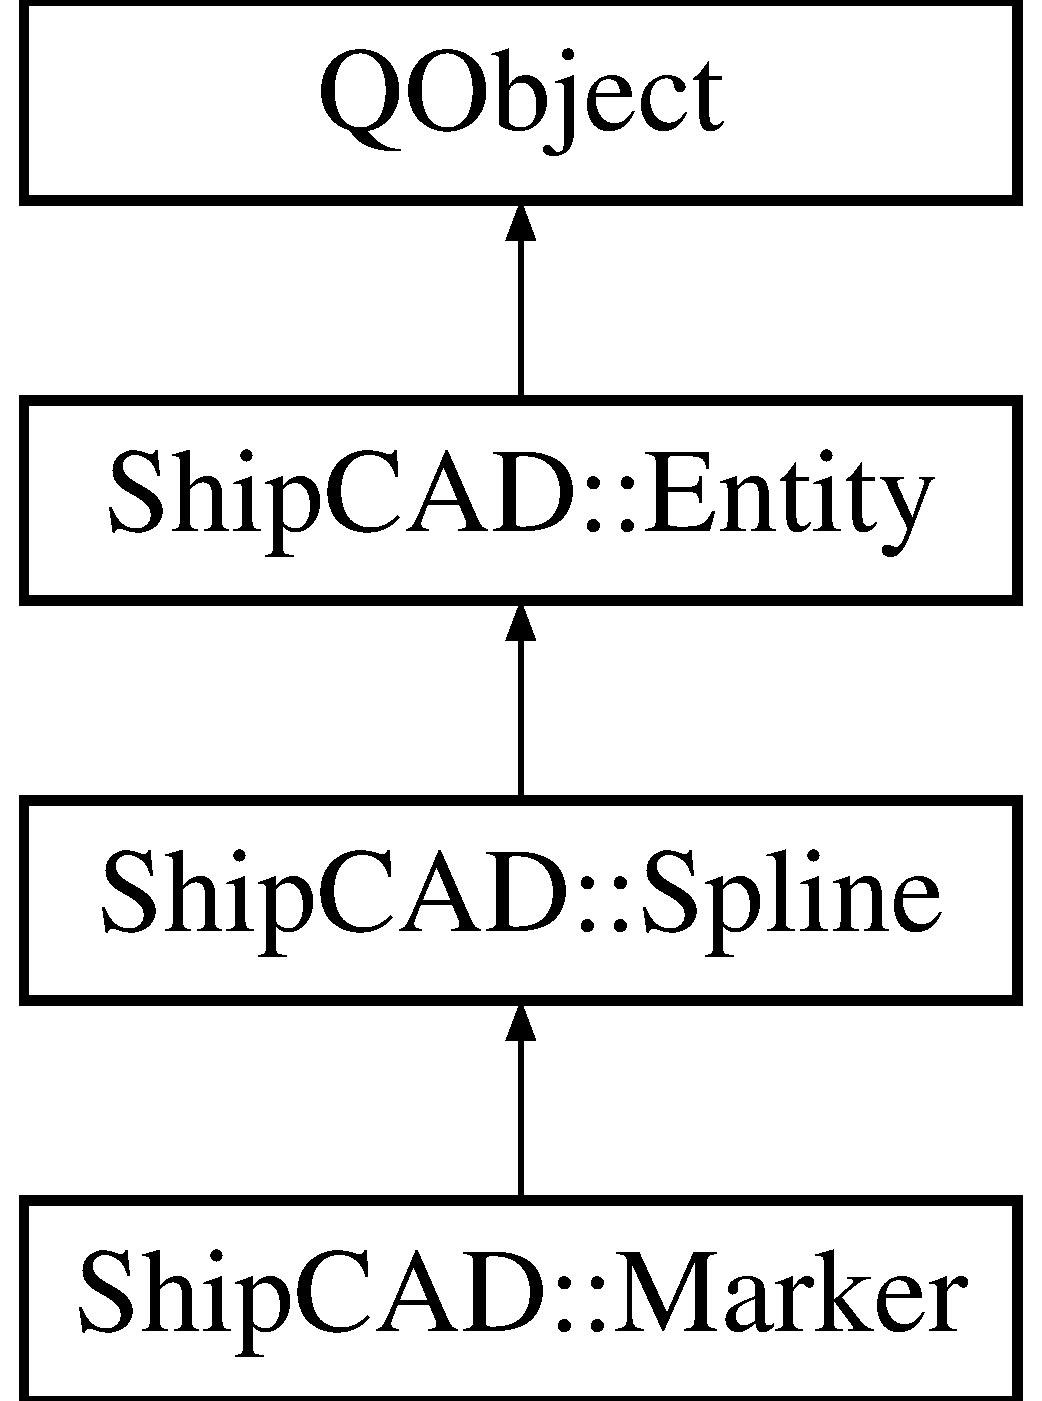
\includegraphics[height=4.000000cm]{classShipCAD_1_1Spline}
\end{center}
\end{figure}
\subsection*{Public Member Functions}
\begin{DoxyCompactItemize}
\item 
\hyperlink{classShipCAD_1_1Spline_a7ad84ea604562c7c9cb309b4e78e25c5}{Spline} ()
\item 
virtual \hyperlink{classShipCAD_1_1Spline_a0c900ca3c99987532e1d0c21ba992968}{$\sim$\-Spline} ()
\item 
void \hyperlink{classShipCAD_1_1Spline_ac3d9f4514573be91b316413bf062791a}{add} (const Q\-Vector3\-D \&p)
\item 
void \hyperlink{classShipCAD_1_1Spline_a120c5530571f138daad61426053220f3}{delete\-\_\-point} (size\-\_\-t index)
\item 
void \hyperlink{classShipCAD_1_1Spline_aa1ea6446e0b59d5cce88580242cd25b6}{insert} (size\-\_\-t index, const Q\-Vector3\-D \&p)
\item 
void \hyperlink{classShipCAD_1_1Spline_aa8e588b92d23c74bb6ec120624b49e54}{insert\-\_\-spline} (size\-\_\-t index, bool invert, bool duplicate\-\_\-point, const \hyperlink{classShipCAD_1_1Spline}{Spline} \&source)
\item 
void \hyperlink{classShipCAD_1_1Spline_a26293a4ee636c2b968c45731425d5c94}{invert\-\_\-direction} ()
\item 
bool \hyperlink{classShipCAD_1_1Spline_a043f418b363a0dc7161b9106a72ef8b4}{simplify} (float criterium)
\item 
virtual void \hyperlink{classShipCAD_1_1Spline_a02967f3eee8b1755eab0d7da55c3c621}{clear} ()
\item 
virtual void \hyperlink{classShipCAD_1_1Spline_a9b466ad7510032dafb0421f2d834bde6}{rebuild} ()
\item 
float \hyperlink{classShipCAD_1_1Spline_a9d4d64a34b1511efc5c41b9e31956a3e}{coord\-\_\-length} (float t1, float t2)
\item 
float \hyperlink{classShipCAD_1_1Spline_ae15513771d88f4f545048d4204e98325}{chord\-\_\-length\-\_\-approximation} (float percentage)
\item 
float \hyperlink{classShipCAD_1_1Spline_a5681a27480f934a73462e53b2b4e2461}{curvature} (float parameter, Q\-Vector3\-D \&normal)
\item 
Q\-Vector3\-D \hyperlink{classShipCAD_1_1Spline_afe15664ac97d1d3452d5a5cfd023c471}{first\-\_\-derive} (float parameter)
\item 
Q\-Vector3\-D \hyperlink{classShipCAD_1_1Spline_abe04c117432e350f3a9f66395d2d3037}{second\-\_\-derive} (float parameter)
\item 
bool \hyperlink{classShipCAD_1_1Spline_afd932e0c63a3b03200ecdc7c656be8e4}{intersect\-\_\-plane} (const \hyperlink{classShipCAD_1_1Plane}{Plane} \&plane, \hyperlink{classShipCAD_1_1IntersectionData}{Intersection\-Data} \&output)
\item 
Q\-Vector3\-D \hyperlink{classShipCAD_1_1Spline_a589d6d945e0fbb905ea94907cd216165}{value} (float parameter)
\item 
virtual void \hyperlink{classShipCAD_1_1Spline_ae90c8807fb8058d6309f47db64e2d40e}{load\-Binary} (\hyperlink{classShipCAD_1_1FileBuffer}{File\-Buffer} \&source)
\item 
virtual void \hyperlink{classShipCAD_1_1Spline_abaf1c6eebdfe8abd41287c1fcb38a808}{save\-Binary} (\hyperlink{classShipCAD_1_1FileBuffer}{File\-Buffer} \&destination)
\item 
void \hyperlink{classShipCAD_1_1Spline_a347502f38c64a12fc19a95e19aad5d7d}{save\-To\-D\-X\-F} (std\-::vector$<$ Q\-String $>$ \&strings, Q\-String layername, bool sendmirror)
\item 
virtual void \hyperlink{classShipCAD_1_1Spline_a6424ed433d241f566c15891cc25a74dd}{draw} (\hyperlink{classShipCAD_1_1Viewport}{Viewport} \&vp, \hyperlink{classShipCAD_1_1LineShader}{Line\-Shader} $\ast$lineshader)
\item 
bool \hyperlink{classShipCAD_1_1Spline_a2c232b5ca5da62ba07ec9aa8ede3fd17}{show\-Curvature} ()
\item 
void \hyperlink{classShipCAD_1_1Spline_aae0f5ce3bc2aa58759abd32f3462bf16}{set\-Show\-Curvature} (bool val)
\item 
Q\-Color \hyperlink{classShipCAD_1_1Spline_ae2e47ccb73a45e0f0d2df2484ba509ae}{get\-Curvature\-Color} ()
\item 
void \hyperlink{classShipCAD_1_1Spline_ac40c22712433f98d657ecaed459d03a0}{set\-Curvature\-Color} (const Q\-Color \&val)
\item 
float \hyperlink{classShipCAD_1_1Spline_ade326d9cd43b6523516b1113b0bddd1b}{get\-Curvature\-Scale} ()
\item 
void \hyperlink{classShipCAD_1_1Spline_a17ba0378bfd4a39b4d96d914332c26e4}{set\-Curvature\-Scale} (float val)
\item 
float \hyperlink{classShipCAD_1_1Spline_ac617856776bb267bdab050b56de4ec74}{get\-Parameter} (size\-\_\-t index)
\item 
Q\-Vector3\-D \hyperlink{classShipCAD_1_1Spline_ad316be28cfd23e518f9e761c46644440}{get\-Point} (size\-\_\-t index)
\item 
void \hyperlink{classShipCAD_1_1Spline_ae02af8d5473f952644ac5103d7beebf2}{set\-Point} (size\-\_\-t index, const Q\-Vector3\-D \&p)
\item 
int \hyperlink{classShipCAD_1_1Spline_a489b034b416be54fe323ad021620f820}{get\-Fragments} ()
\item 
void \hyperlink{classShipCAD_1_1Spline_aaae6e558fad0833cde71f9ed38e4fb96}{set\-Fragments} (size\-\_\-t val)
\item 
bool \hyperlink{classShipCAD_1_1Spline_a90a954f52321f3b1b27b43991e9997a5}{is\-Knuckle} (size\-\_\-t index)
\item 
void \hyperlink{classShipCAD_1_1Spline_ad4f075e2e8f1d3ac7c2d22b5be75bbad}{set\-Knuckle} (size\-\_\-t index, bool val)
\item 
size\-\_\-t \hyperlink{classShipCAD_1_1Spline_ae22e067eaf100aca4cd4262e283ec089}{number\-Of\-Points} ()
\item 
void \hyperlink{classShipCAD_1_1Spline_a156ffe855d149ad445b178078ee4451c}{dump} (std\-::ostream \&os) const 
\end{DoxyCompactItemize}
\subsection*{Protected Member Functions}
\begin{DoxyCompactItemize}
\item 
void \hyperlink{classShipCAD_1_1Spline_a6e932411f0f4463514f80011c58f5e6a}{set\-Build} (bool val)
\item 
float \hyperlink{classShipCAD_1_1Spline_a63165f7cf70338e51b0f16504366031e}{weight} (size\-\_\-t index)
\item 
std\-::vector$<$ float $>$\-::iterator \hyperlink{classShipCAD_1_1Spline_a20b39f3a1bd853040df4760cd912ee64}{find\-\_\-next\-\_\-point} (std\-::vector$<$ float $>$ \&weights)
\item 
void \hyperlink{classShipCAD_1_1Spline_ab8f0b98595ccbd62e754fe92354a207b}{add\-\_\-to\-\_\-output} (const Q\-Vector3\-D \&p, float parameter, \hyperlink{classShipCAD_1_1IntersectionData}{Intersection\-Data} \&output)
\end{DoxyCompactItemize}
\subsection*{Protected Attributes}
\begin{DoxyCompactItemize}
\item 
size\-\_\-t \hyperlink{classShipCAD_1_1Spline_a94ae8704ab2cae5ba6bb915e3df2e98d}{\-\_\-nopoints}
\item 
size\-\_\-t \hyperlink{classShipCAD_1_1Spline_ac12e47ffb75b6d84877f849d18323622}{\-\_\-fragments}
\item 
bool \hyperlink{classShipCAD_1_1Spline_a5b5ebff933cd6fc2d59e0412bf342591}{\-\_\-show\-\_\-curvature}
\item 
bool \hyperlink{classShipCAD_1_1Spline_af850b71f44eaced42ede035d73cb4271}{\-\_\-show\-\_\-points}
\item 
float \hyperlink{classShipCAD_1_1Spline_ac9b097c34a061077a02fc9e1563b3e86}{\-\_\-curvature\-\_\-scale}
\item 
Q\-Color \hyperlink{classShipCAD_1_1Spline_add77b6dfe1a27c34602b3d2f576be7f4}{\-\_\-curvature\-\_\-color}
\item 
std\-::vector$<$ Q\-Vector3\-D $>$ \hyperlink{classShipCAD_1_1Spline_a6288af72f907a160974b7ce5207316ec}{\-\_\-points}
\item 
std\-::vector$<$ bool $>$ \hyperlink{classShipCAD_1_1Spline_ac7d024ce90642d78587bc921efde009c}{\-\_\-knuckles}
\item 
float \hyperlink{classShipCAD_1_1Spline_ae9e5a60e0a8722d9a3cd483f6019e4e9}{\-\_\-total\-\_\-length}
\item 
std\-::vector$<$ float $>$ \hyperlink{classShipCAD_1_1Spline_a374180992c17d3ee4b869d45080529fc}{\-\_\-parameters}
\item 
std\-::vector$<$ Q\-Vector3\-D $>$ \hyperlink{classShipCAD_1_1Spline_a8478f85abd680e3caee34dc230eed3e7}{\-\_\-derivatives}
\end{DoxyCompactItemize}
\subsection*{Properties}
\begin{DoxyCompactItemize}
\item 
size\-\_\-t \hyperlink{classShipCAD_1_1Spline_a5e4df2a54955094c035f32a442602afc}{Fragments}
\item 
bool \hyperlink{classShipCAD_1_1Spline_a9572e31014a04689a2987475c9bff080}{Show\-Curvature}
\item 
bool \hyperlink{classShipCAD_1_1Spline_abac1aad3fc0e33ea8ccda1a94bea8467}{Show\-Points}
\item 
float \hyperlink{classShipCAD_1_1Spline_a5e8a93a4b5d164f38773e7edbf7753b3}{Curvature\-Scale}
\item 
Q\-Color \hyperlink{classShipCAD_1_1Spline_ac5268eaa6aadac5db072c7fdeb578ed4}{Curvature\-Color}
\end{DoxyCompactItemize}


\subsection{Detailed Description}


Definition at line 50 of file spline.\-h.



\subsection{Constructor \& Destructor Documentation}
\hypertarget{classShipCAD_1_1Spline_a7ad84ea604562c7c9cb309b4e78e25c5}{\index{Ship\-C\-A\-D\-::\-Spline@{Ship\-C\-A\-D\-::\-Spline}!Spline@{Spline}}
\index{Spline@{Spline}!ShipCAD::Spline@{Ship\-C\-A\-D\-::\-Spline}}
\subsubsection[{Spline}]{\setlength{\rightskip}{0pt plus 5cm}Spline\-::\-Spline (
\begin{DoxyParamCaption}
{}
\end{DoxyParamCaption}
)\hspace{0.3cm}{\ttfamily [explicit]}}}\label{classShipCAD_1_1Spline_a7ad84ea604562c7c9cb309b4e78e25c5}


Definition at line 50 of file spline.\-cpp.

\hypertarget{classShipCAD_1_1Spline_a0c900ca3c99987532e1d0c21ba992968}{\index{Ship\-C\-A\-D\-::\-Spline@{Ship\-C\-A\-D\-::\-Spline}!$\sim$\-Spline@{$\sim$\-Spline}}
\index{$\sim$\-Spline@{$\sim$\-Spline}!ShipCAD::Spline@{Ship\-C\-A\-D\-::\-Spline}}
\subsubsection[{$\sim$\-Spline}]{\setlength{\rightskip}{0pt plus 5cm}Spline\-::$\sim$\-Spline (
\begin{DoxyParamCaption}
{}
\end{DoxyParamCaption}
)\hspace{0.3cm}{\ttfamily [virtual]}}}\label{classShipCAD_1_1Spline_a0c900ca3c99987532e1d0c21ba992968}


Definition at line 56 of file spline.\-cpp.



\subsection{Member Function Documentation}
\hypertarget{classShipCAD_1_1Spline_ac3d9f4514573be91b316413bf062791a}{\index{Ship\-C\-A\-D\-::\-Spline@{Ship\-C\-A\-D\-::\-Spline}!add@{add}}
\index{add@{add}!ShipCAD::Spline@{Ship\-C\-A\-D\-::\-Spline}}
\subsubsection[{add}]{\setlength{\rightskip}{0pt plus 5cm}void Spline\-::add (
\begin{DoxyParamCaption}
\item[{const Q\-Vector3\-D \&}]{p}
\end{DoxyParamCaption}
)}}\label{classShipCAD_1_1Spline_ac3d9f4514573be91b316413bf062791a}


Definition at line 387 of file spline.\-cpp.

\hypertarget{classShipCAD_1_1Spline_ab8f0b98595ccbd62e754fe92354a207b}{\index{Ship\-C\-A\-D\-::\-Spline@{Ship\-C\-A\-D\-::\-Spline}!add\-\_\-to\-\_\-output@{add\-\_\-to\-\_\-output}}
\index{add\-\_\-to\-\_\-output@{add\-\_\-to\-\_\-output}!ShipCAD::Spline@{Ship\-C\-A\-D\-::\-Spline}}
\subsubsection[{add\-\_\-to\-\_\-output}]{\setlength{\rightskip}{0pt plus 5cm}void Spline\-::add\-\_\-to\-\_\-output (
\begin{DoxyParamCaption}
\item[{const Q\-Vector3\-D \&}]{p, }
\item[{float}]{parameter, }
\item[{{\bf Intersection\-Data} \&}]{output}
\end{DoxyParamCaption}
)\hspace{0.3cm}{\ttfamily [protected]}}}\label{classShipCAD_1_1Spline_ab8f0b98595ccbd62e754fe92354a207b}


Definition at line 608 of file spline.\-cpp.

\hypertarget{classShipCAD_1_1Spline_ae15513771d88f4f545048d4204e98325}{\index{Ship\-C\-A\-D\-::\-Spline@{Ship\-C\-A\-D\-::\-Spline}!chord\-\_\-length\-\_\-approximation@{chord\-\_\-length\-\_\-approximation}}
\index{chord\-\_\-length\-\_\-approximation@{chord\-\_\-length\-\_\-approximation}!ShipCAD::Spline@{Ship\-C\-A\-D\-::\-Spline}}
\subsubsection[{chord\-\_\-length\-\_\-approximation}]{\setlength{\rightskip}{0pt plus 5cm}float Spline\-::chord\-\_\-length\-\_\-approximation (
\begin{DoxyParamCaption}
\item[{float}]{percentage}
\end{DoxyParamCaption}
)}}\label{classShipCAD_1_1Spline_ae15513771d88f4f545048d4204e98325}


Definition at line 415 of file spline.\-cpp.

\hypertarget{classShipCAD_1_1Spline_a02967f3eee8b1755eab0d7da55c3c621}{\index{Ship\-C\-A\-D\-::\-Spline@{Ship\-C\-A\-D\-::\-Spline}!clear@{clear}}
\index{clear@{clear}!ShipCAD::Spline@{Ship\-C\-A\-D\-::\-Spline}}
\subsubsection[{clear}]{\setlength{\rightskip}{0pt plus 5cm}void Spline\-::clear (
\begin{DoxyParamCaption}
{}
\end{DoxyParamCaption}
)\hspace{0.3cm}{\ttfamily [virtual]}}}\label{classShipCAD_1_1Spline_a02967f3eee8b1755eab0d7da55c3c621}


Reimplemented from \hyperlink{classShipCAD_1_1Entity_a998d0e5d360371046fd5835ba1e0877a}{Ship\-C\-A\-D\-::\-Entity}.



Reimplemented in \hyperlink{classShipCAD_1_1Marker_ac7c7eea8648562f3fa00a9e10af6ec97}{Ship\-C\-A\-D\-::\-Marker}.



Definition at line 730 of file spline.\-cpp.

\hypertarget{classShipCAD_1_1Spline_a9d4d64a34b1511efc5c41b9e31956a3e}{\index{Ship\-C\-A\-D\-::\-Spline@{Ship\-C\-A\-D\-::\-Spline}!coord\-\_\-length@{coord\-\_\-length}}
\index{coord\-\_\-length@{coord\-\_\-length}!ShipCAD::Spline@{Ship\-C\-A\-D\-::\-Spline}}
\subsubsection[{coord\-\_\-length}]{\setlength{\rightskip}{0pt plus 5cm}float Spline\-::coord\-\_\-length (
\begin{DoxyParamCaption}
\item[{float}]{t1, }
\item[{float}]{t2}
\end{DoxyParamCaption}
)}}\label{classShipCAD_1_1Spline_a9d4d64a34b1511efc5c41b9e31956a3e}


Definition at line 395 of file spline.\-cpp.

\hypertarget{classShipCAD_1_1Spline_a5681a27480f934a73462e53b2b4e2461}{\index{Ship\-C\-A\-D\-::\-Spline@{Ship\-C\-A\-D\-::\-Spline}!curvature@{curvature}}
\index{curvature@{curvature}!ShipCAD::Spline@{Ship\-C\-A\-D\-::\-Spline}}
\subsubsection[{curvature}]{\setlength{\rightskip}{0pt plus 5cm}float Spline\-::curvature (
\begin{DoxyParamCaption}
\item[{float}]{parameter, }
\item[{Q\-Vector3\-D \&}]{normal}
\end{DoxyParamCaption}
)}}\label{classShipCAD_1_1Spline_a5681a27480f934a73462e53b2b4e2461}


Definition at line 463 of file spline.\-cpp.

\hypertarget{classShipCAD_1_1Spline_a120c5530571f138daad61426053220f3}{\index{Ship\-C\-A\-D\-::\-Spline@{Ship\-C\-A\-D\-::\-Spline}!delete\-\_\-point@{delete\-\_\-point}}
\index{delete\-\_\-point@{delete\-\_\-point}!ShipCAD::Spline@{Ship\-C\-A\-D\-::\-Spline}}
\subsubsection[{delete\-\_\-point}]{\setlength{\rightskip}{0pt plus 5cm}void Spline\-::delete\-\_\-point (
\begin{DoxyParamCaption}
\item[{size\-\_\-t}]{index}
\end{DoxyParamCaption}
)}}\label{classShipCAD_1_1Spline_a120c5530571f138daad61426053220f3}


Definition at line 485 of file spline.\-cpp.

\hypertarget{classShipCAD_1_1Spline_a6424ed433d241f566c15891cc25a74dd}{\index{Ship\-C\-A\-D\-::\-Spline@{Ship\-C\-A\-D\-::\-Spline}!draw@{draw}}
\index{draw@{draw}!ShipCAD::Spline@{Ship\-C\-A\-D\-::\-Spline}}
\subsubsection[{draw}]{\setlength{\rightskip}{0pt plus 5cm}void Spline\-::draw (
\begin{DoxyParamCaption}
\item[{{\bf Viewport} \&}]{vp, }
\item[{{\bf Line\-Shader} $\ast$}]{lineshader}
\end{DoxyParamCaption}
)\hspace{0.3cm}{\ttfamily [virtual]}}}\label{classShipCAD_1_1Spline_a6424ed433d241f566c15891cc25a74dd}


Implements \hyperlink{classShipCAD_1_1Entity_aa62e306d991140dcd564360f8f6e7539}{Ship\-C\-A\-D\-::\-Entity}.



Reimplemented in \hyperlink{classShipCAD_1_1Marker_a0cca647d9b32dc69b03903b024dc3091}{Ship\-C\-A\-D\-::\-Marker}.



Definition at line 523 of file spline.\-cpp.

\hypertarget{classShipCAD_1_1Spline_a156ffe855d149ad445b178078ee4451c}{\index{Ship\-C\-A\-D\-::\-Spline@{Ship\-C\-A\-D\-::\-Spline}!dump@{dump}}
\index{dump@{dump}!ShipCAD::Spline@{Ship\-C\-A\-D\-::\-Spline}}
\subsubsection[{dump}]{\setlength{\rightskip}{0pt plus 5cm}void Spline\-::dump (
\begin{DoxyParamCaption}
\item[{std\-::ostream \&}]{os}
\end{DoxyParamCaption}
) const}}\label{classShipCAD_1_1Spline_a156ffe855d149ad445b178078ee4451c}


Definition at line 789 of file spline.\-cpp.

\hypertarget{classShipCAD_1_1Spline_a20b39f3a1bd853040df4760cd912ee64}{\index{Ship\-C\-A\-D\-::\-Spline@{Ship\-C\-A\-D\-::\-Spline}!find\-\_\-next\-\_\-point@{find\-\_\-next\-\_\-point}}
\index{find\-\_\-next\-\_\-point@{find\-\_\-next\-\_\-point}!ShipCAD::Spline@{Ship\-C\-A\-D\-::\-Spline}}
\subsubsection[{find\-\_\-next\-\_\-point}]{\setlength{\rightskip}{0pt plus 5cm}vector$<$ float $>$\-::iterator Spline\-::find\-\_\-next\-\_\-point (
\begin{DoxyParamCaption}
\item[{std\-::vector$<$ float $>$ \&}]{weights}
\end{DoxyParamCaption}
)\hspace{0.3cm}{\ttfamily [protected]}}}\label{classShipCAD_1_1Spline_a20b39f3a1bd853040df4760cd912ee64}


Definition at line 324 of file spline.\-cpp.

\hypertarget{classShipCAD_1_1Spline_afe15664ac97d1d3452d5a5cfd023c471}{\index{Ship\-C\-A\-D\-::\-Spline@{Ship\-C\-A\-D\-::\-Spline}!first\-\_\-derive@{first\-\_\-derive}}
\index{first\-\_\-derive@{first\-\_\-derive}!ShipCAD::Spline@{Ship\-C\-A\-D\-::\-Spline}}
\subsubsection[{first\-\_\-derive}]{\setlength{\rightskip}{0pt plus 5cm}Q\-Vector3\-D Spline\-::first\-\_\-derive (
\begin{DoxyParamCaption}
\item[{float}]{parameter}
\end{DoxyParamCaption}
)}}\label{classShipCAD_1_1Spline_afe15664ac97d1d3452d5a5cfd023c471}


Definition at line 495 of file spline.\-cpp.

\hypertarget{classShipCAD_1_1Spline_ae2e47ccb73a45e0f0d2df2484ba509ae}{\index{Ship\-C\-A\-D\-::\-Spline@{Ship\-C\-A\-D\-::\-Spline}!get\-Curvature\-Color@{get\-Curvature\-Color}}
\index{get\-Curvature\-Color@{get\-Curvature\-Color}!ShipCAD::Spline@{Ship\-C\-A\-D\-::\-Spline}}
\subsubsection[{get\-Curvature\-Color}]{\setlength{\rightskip}{0pt plus 5cm}Q\-Color Ship\-C\-A\-D\-::\-Spline\-::get\-Curvature\-Color (
\begin{DoxyParamCaption}
{}
\end{DoxyParamCaption}
)\hspace{0.3cm}{\ttfamily [inline]}}}\label{classShipCAD_1_1Spline_ae2e47ccb73a45e0f0d2df2484ba509ae}


Definition at line 98 of file spline.\-h.

\hypertarget{classShipCAD_1_1Spline_ade326d9cd43b6523516b1113b0bddd1b}{\index{Ship\-C\-A\-D\-::\-Spline@{Ship\-C\-A\-D\-::\-Spline}!get\-Curvature\-Scale@{get\-Curvature\-Scale}}
\index{get\-Curvature\-Scale@{get\-Curvature\-Scale}!ShipCAD::Spline@{Ship\-C\-A\-D\-::\-Spline}}
\subsubsection[{get\-Curvature\-Scale}]{\setlength{\rightskip}{0pt plus 5cm}float Ship\-C\-A\-D\-::\-Spline\-::get\-Curvature\-Scale (
\begin{DoxyParamCaption}
{}
\end{DoxyParamCaption}
)\hspace{0.3cm}{\ttfamily [inline]}}}\label{classShipCAD_1_1Spline_ade326d9cd43b6523516b1113b0bddd1b}


Definition at line 100 of file spline.\-h.

\hypertarget{classShipCAD_1_1Spline_a489b034b416be54fe323ad021620f820}{\index{Ship\-C\-A\-D\-::\-Spline@{Ship\-C\-A\-D\-::\-Spline}!get\-Fragments@{get\-Fragments}}
\index{get\-Fragments@{get\-Fragments}!ShipCAD::Spline@{Ship\-C\-A\-D\-::\-Spline}}
\subsubsection[{get\-Fragments}]{\setlength{\rightskip}{0pt plus 5cm}int Spline\-::get\-Fragments (
\begin{DoxyParamCaption}
{}
\end{DoxyParamCaption}
)}}\label{classShipCAD_1_1Spline_a489b034b416be54fe323ad021620f820}


Definition at line 81 of file spline.\-cpp.

\hypertarget{classShipCAD_1_1Spline_ac617856776bb267bdab050b56de4ec74}{\index{Ship\-C\-A\-D\-::\-Spline@{Ship\-C\-A\-D\-::\-Spline}!get\-Parameter@{get\-Parameter}}
\index{get\-Parameter@{get\-Parameter}!ShipCAD::Spline@{Ship\-C\-A\-D\-::\-Spline}}
\subsubsection[{get\-Parameter}]{\setlength{\rightskip}{0pt plus 5cm}float Spline\-::get\-Parameter (
\begin{DoxyParamCaption}
\item[{size\-\_\-t}]{index}
\end{DoxyParamCaption}
)}}\label{classShipCAD_1_1Spline_ac617856776bb267bdab050b56de4ec74}


Definition at line 115 of file spline.\-cpp.

\hypertarget{classShipCAD_1_1Spline_ad316be28cfd23e518f9e761c46644440}{\index{Ship\-C\-A\-D\-::\-Spline@{Ship\-C\-A\-D\-::\-Spline}!get\-Point@{get\-Point}}
\index{get\-Point@{get\-Point}!ShipCAD::Spline@{Ship\-C\-A\-D\-::\-Spline}}
\subsubsection[{get\-Point}]{\setlength{\rightskip}{0pt plus 5cm}Q\-Vector3\-D Spline\-::get\-Point (
\begin{DoxyParamCaption}
\item[{size\-\_\-t}]{index}
\end{DoxyParamCaption}
)}}\label{classShipCAD_1_1Spline_ad316be28cfd23e518f9e761c46644440}


Definition at line 125 of file spline.\-cpp.

\hypertarget{classShipCAD_1_1Spline_aa1ea6446e0b59d5cce88580242cd25b6}{\index{Ship\-C\-A\-D\-::\-Spline@{Ship\-C\-A\-D\-::\-Spline}!insert@{insert}}
\index{insert@{insert}!ShipCAD::Spline@{Ship\-C\-A\-D\-::\-Spline}}
\subsubsection[{insert}]{\setlength{\rightskip}{0pt plus 5cm}void Spline\-::insert (
\begin{DoxyParamCaption}
\item[{size\-\_\-t}]{index, }
\item[{const Q\-Vector3\-D \&}]{p}
\end{DoxyParamCaption}
)}}\label{classShipCAD_1_1Spline_aa1ea6446e0b59d5cce88580242cd25b6}


Definition at line 511 of file spline.\-cpp.

\hypertarget{classShipCAD_1_1Spline_aa8e588b92d23c74bb6ec120624b49e54}{\index{Ship\-C\-A\-D\-::\-Spline@{Ship\-C\-A\-D\-::\-Spline}!insert\-\_\-spline@{insert\-\_\-spline}}
\index{insert\-\_\-spline@{insert\-\_\-spline}!ShipCAD::Spline@{Ship\-C\-A\-D\-::\-Spline}}
\subsubsection[{insert\-\_\-spline}]{\setlength{\rightskip}{0pt plus 5cm}void Spline\-::insert\-\_\-spline (
\begin{DoxyParamCaption}
\item[{size\-\_\-t}]{index, }
\item[{bool}]{invert, }
\item[{bool}]{duplicate\-\_\-point, }
\item[{const {\bf Spline} \&}]{source}
\end{DoxyParamCaption}
)}}\label{classShipCAD_1_1Spline_aa8e588b92d23c74bb6ec120624b49e54}


Definition at line 580 of file spline.\-cpp.

\hypertarget{classShipCAD_1_1Spline_afd932e0c63a3b03200ecdc7c656be8e4}{\index{Ship\-C\-A\-D\-::\-Spline@{Ship\-C\-A\-D\-::\-Spline}!intersect\-\_\-plane@{intersect\-\_\-plane}}
\index{intersect\-\_\-plane@{intersect\-\_\-plane}!ShipCAD::Spline@{Ship\-C\-A\-D\-::\-Spline}}
\subsubsection[{intersect\-\_\-plane}]{\setlength{\rightskip}{0pt plus 5cm}bool Spline\-::intersect\-\_\-plane (
\begin{DoxyParamCaption}
\item[{const {\bf Plane} \&}]{plane, }
\item[{{\bf Intersection\-Data} \&}]{output}
\end{DoxyParamCaption}
)}}\label{classShipCAD_1_1Spline_afd932e0c63a3b03200ecdc7c656be8e4}


Definition at line 615 of file spline.\-cpp.

\hypertarget{classShipCAD_1_1Spline_a26293a4ee636c2b968c45731425d5c94}{\index{Ship\-C\-A\-D\-::\-Spline@{Ship\-C\-A\-D\-::\-Spline}!invert\-\_\-direction@{invert\-\_\-direction}}
\index{invert\-\_\-direction@{invert\-\_\-direction}!ShipCAD::Spline@{Ship\-C\-A\-D\-::\-Spline}}
\subsubsection[{invert\-\_\-direction}]{\setlength{\rightskip}{0pt plus 5cm}void Spline\-::invert\-\_\-direction (
\begin{DoxyParamCaption}
{}
\end{DoxyParamCaption}
)}}\label{classShipCAD_1_1Spline_a26293a4ee636c2b968c45731425d5c94}


Definition at line 642 of file spline.\-cpp.

\hypertarget{classShipCAD_1_1Spline_a90a954f52321f3b1b27b43991e9997a5}{\index{Ship\-C\-A\-D\-::\-Spline@{Ship\-C\-A\-D\-::\-Spline}!is\-Knuckle@{is\-Knuckle}}
\index{is\-Knuckle@{is\-Knuckle}!ShipCAD::Spline@{Ship\-C\-A\-D\-::\-Spline}}
\subsubsection[{is\-Knuckle}]{\setlength{\rightskip}{0pt plus 5cm}bool Spline\-::is\-Knuckle (
\begin{DoxyParamCaption}
\item[{size\-\_\-t}]{index}
\end{DoxyParamCaption}
)}}\label{classShipCAD_1_1Spline_a90a954f52321f3b1b27b43991e9997a5}


Definition at line 86 of file spline.\-cpp.

\hypertarget{classShipCAD_1_1Spline_ae90c8807fb8058d6309f47db64e2d40e}{\index{Ship\-C\-A\-D\-::\-Spline@{Ship\-C\-A\-D\-::\-Spline}!load\-Binary@{load\-Binary}}
\index{load\-Binary@{load\-Binary}!ShipCAD::Spline@{Ship\-C\-A\-D\-::\-Spline}}
\subsubsection[{load\-Binary}]{\setlength{\rightskip}{0pt plus 5cm}void Spline\-::load\-Binary (
\begin{DoxyParamCaption}
\item[{{\bf File\-Buffer} \&}]{source}
\end{DoxyParamCaption}
)\hspace{0.3cm}{\ttfamily [virtual]}}}\label{classShipCAD_1_1Spline_ae90c8807fb8058d6309f47db64e2d40e}


Reimplemented in \hyperlink{classShipCAD_1_1Marker_a0f2aa7cd6bae40784c077b89d5ebdb50}{Ship\-C\-A\-D\-::\-Marker}.



Definition at line 653 of file spline.\-cpp.

\hypertarget{classShipCAD_1_1Spline_ae22e067eaf100aca4cd4262e283ec089}{\index{Ship\-C\-A\-D\-::\-Spline@{Ship\-C\-A\-D\-::\-Spline}!number\-Of\-Points@{number\-Of\-Points}}
\index{number\-Of\-Points@{number\-Of\-Points}!ShipCAD::Spline@{Ship\-C\-A\-D\-::\-Spline}}
\subsubsection[{number\-Of\-Points}]{\setlength{\rightskip}{0pt plus 5cm}size\-\_\-t Ship\-C\-A\-D\-::\-Spline\-::number\-Of\-Points (
\begin{DoxyParamCaption}
{}
\end{DoxyParamCaption}
)\hspace{0.3cm}{\ttfamily [inline]}}}\label{classShipCAD_1_1Spline_ae22e067eaf100aca4cd4262e283ec089}


Definition at line 109 of file spline.\-h.

\hypertarget{classShipCAD_1_1Spline_a9b466ad7510032dafb0421f2d834bde6}{\index{Ship\-C\-A\-D\-::\-Spline@{Ship\-C\-A\-D\-::\-Spline}!rebuild@{rebuild}}
\index{rebuild@{rebuild}!ShipCAD::Spline@{Ship\-C\-A\-D\-::\-Spline}}
\subsubsection[{rebuild}]{\setlength{\rightskip}{0pt plus 5cm}void Spline\-::rebuild (
\begin{DoxyParamCaption}
{}
\end{DoxyParamCaption}
)\hspace{0.3cm}{\ttfamily [virtual]}}}\label{classShipCAD_1_1Spline_a9b466ad7510032dafb0421f2d834bde6}


Implements \hyperlink{classShipCAD_1_1Entity_a2571654319df6ad6841a437be7a75395}{Ship\-C\-A\-D\-::\-Entity}.



Definition at line 135 of file spline.\-cpp.

\hypertarget{classShipCAD_1_1Spline_abaf1c6eebdfe8abd41287c1fcb38a808}{\index{Ship\-C\-A\-D\-::\-Spline@{Ship\-C\-A\-D\-::\-Spline}!save\-Binary@{save\-Binary}}
\index{save\-Binary@{save\-Binary}!ShipCAD::Spline@{Ship\-C\-A\-D\-::\-Spline}}
\subsubsection[{save\-Binary}]{\setlength{\rightskip}{0pt plus 5cm}void Spline\-::save\-Binary (
\begin{DoxyParamCaption}
\item[{{\bf File\-Buffer} \&}]{destination}
\end{DoxyParamCaption}
)\hspace{0.3cm}{\ttfamily [virtual]}}}\label{classShipCAD_1_1Spline_abaf1c6eebdfe8abd41287c1fcb38a808}


Reimplemented in \hyperlink{classShipCAD_1_1Marker_abceb4cbb5b038eb88d0f7f26507be15c}{Ship\-C\-A\-D\-::\-Marker}.



Definition at line 669 of file spline.\-cpp.

\hypertarget{classShipCAD_1_1Spline_a347502f38c64a12fc19a95e19aad5d7d}{\index{Ship\-C\-A\-D\-::\-Spline@{Ship\-C\-A\-D\-::\-Spline}!save\-To\-D\-X\-F@{save\-To\-D\-X\-F}}
\index{save\-To\-D\-X\-F@{save\-To\-D\-X\-F}!ShipCAD::Spline@{Ship\-C\-A\-D\-::\-Spline}}
\subsubsection[{save\-To\-D\-X\-F}]{\setlength{\rightskip}{0pt plus 5cm}void Spline\-::save\-To\-D\-X\-F (
\begin{DoxyParamCaption}
\item[{std\-::vector$<$ Q\-String $>$ \&}]{strings, }
\item[{Q\-String}]{layername, }
\item[{bool}]{sendmirror}
\end{DoxyParamCaption}
)}}\label{classShipCAD_1_1Spline_a347502f38c64a12fc19a95e19aad5d7d}


Definition at line 680 of file spline.\-cpp.

\hypertarget{classShipCAD_1_1Spline_abe04c117432e350f3a9f66395d2d3037}{\index{Ship\-C\-A\-D\-::\-Spline@{Ship\-C\-A\-D\-::\-Spline}!second\-\_\-derive@{second\-\_\-derive}}
\index{second\-\_\-derive@{second\-\_\-derive}!ShipCAD::Spline@{Ship\-C\-A\-D\-::\-Spline}}
\subsubsection[{second\-\_\-derive}]{\setlength{\rightskip}{0pt plus 5cm}Q\-Vector3\-D Spline\-::second\-\_\-derive (
\begin{DoxyParamCaption}
\item[{float}]{parameter}
\end{DoxyParamCaption}
)}}\label{classShipCAD_1_1Spline_abe04c117432e350f3a9f66395d2d3037}


Definition at line 255 of file spline.\-cpp.

\hypertarget{classShipCAD_1_1Spline_a6e932411f0f4463514f80011c58f5e6a}{\index{Ship\-C\-A\-D\-::\-Spline@{Ship\-C\-A\-D\-::\-Spline}!set\-Build@{set\-Build}}
\index{set\-Build@{set\-Build}!ShipCAD::Spline@{Ship\-C\-A\-D\-::\-Spline}}
\subsubsection[{set\-Build}]{\setlength{\rightskip}{0pt plus 5cm}void Spline\-::set\-Build (
\begin{DoxyParamCaption}
\item[{bool}]{val}
\end{DoxyParamCaption}
)\hspace{0.3cm}{\ttfamily [protected]}, {\ttfamily [virtual]}}}\label{classShipCAD_1_1Spline_a6e932411f0f4463514f80011c58f5e6a}


Reimplemented from \hyperlink{classShipCAD_1_1Entity_a1889198398f42bb7f77a2334031c3f33}{Ship\-C\-A\-D\-::\-Entity}.



Definition at line 61 of file spline.\-cpp.

\hypertarget{classShipCAD_1_1Spline_ac40c22712433f98d657ecaed459d03a0}{\index{Ship\-C\-A\-D\-::\-Spline@{Ship\-C\-A\-D\-::\-Spline}!set\-Curvature\-Color@{set\-Curvature\-Color}}
\index{set\-Curvature\-Color@{set\-Curvature\-Color}!ShipCAD::Spline@{Ship\-C\-A\-D\-::\-Spline}}
\subsubsection[{set\-Curvature\-Color}]{\setlength{\rightskip}{0pt plus 5cm}void Ship\-C\-A\-D\-::\-Spline\-::set\-Curvature\-Color (
\begin{DoxyParamCaption}
\item[{const Q\-Color \&}]{val}
\end{DoxyParamCaption}
)\hspace{0.3cm}{\ttfamily [inline]}}}\label{classShipCAD_1_1Spline_ac40c22712433f98d657ecaed459d03a0}


Definition at line 99 of file spline.\-h.

\hypertarget{classShipCAD_1_1Spline_a17ba0378bfd4a39b4d96d914332c26e4}{\index{Ship\-C\-A\-D\-::\-Spline@{Ship\-C\-A\-D\-::\-Spline}!set\-Curvature\-Scale@{set\-Curvature\-Scale}}
\index{set\-Curvature\-Scale@{set\-Curvature\-Scale}!ShipCAD::Spline@{Ship\-C\-A\-D\-::\-Spline}}
\subsubsection[{set\-Curvature\-Scale}]{\setlength{\rightskip}{0pt plus 5cm}void Ship\-C\-A\-D\-::\-Spline\-::set\-Curvature\-Scale (
\begin{DoxyParamCaption}
\item[{float}]{val}
\end{DoxyParamCaption}
)\hspace{0.3cm}{\ttfamily [inline]}}}\label{classShipCAD_1_1Spline_a17ba0378bfd4a39b4d96d914332c26e4}


Definition at line 101 of file spline.\-h.

\hypertarget{classShipCAD_1_1Spline_aaae6e558fad0833cde71f9ed38e4fb96}{\index{Ship\-C\-A\-D\-::\-Spline@{Ship\-C\-A\-D\-::\-Spline}!set\-Fragments@{set\-Fragments}}
\index{set\-Fragments@{set\-Fragments}!ShipCAD::Spline@{Ship\-C\-A\-D\-::\-Spline}}
\subsubsection[{set\-Fragments}]{\setlength{\rightskip}{0pt plus 5cm}void Spline\-::set\-Fragments (
\begin{DoxyParamCaption}
\item[{size\-\_\-t}]{val}
\end{DoxyParamCaption}
)}}\label{classShipCAD_1_1Spline_aaae6e558fad0833cde71f9ed38e4fb96}


Definition at line 73 of file spline.\-cpp.

\hypertarget{classShipCAD_1_1Spline_ad4f075e2e8f1d3ac7c2d22b5be75bbad}{\index{Ship\-C\-A\-D\-::\-Spline@{Ship\-C\-A\-D\-::\-Spline}!set\-Knuckle@{set\-Knuckle}}
\index{set\-Knuckle@{set\-Knuckle}!ShipCAD::Spline@{Ship\-C\-A\-D\-::\-Spline}}
\subsubsection[{set\-Knuckle}]{\setlength{\rightskip}{0pt plus 5cm}void Spline\-::set\-Knuckle (
\begin{DoxyParamCaption}
\item[{size\-\_\-t}]{index, }
\item[{bool}]{val}
\end{DoxyParamCaption}
)}}\label{classShipCAD_1_1Spline_ad4f075e2e8f1d3ac7c2d22b5be75bbad}


Definition at line 93 of file spline.\-cpp.

\hypertarget{classShipCAD_1_1Spline_ae02af8d5473f952644ac5103d7beebf2}{\index{Ship\-C\-A\-D\-::\-Spline@{Ship\-C\-A\-D\-::\-Spline}!set\-Point@{set\-Point}}
\index{set\-Point@{set\-Point}!ShipCAD::Spline@{Ship\-C\-A\-D\-::\-Spline}}
\subsubsection[{set\-Point}]{\setlength{\rightskip}{0pt plus 5cm}void Spline\-::set\-Point (
\begin{DoxyParamCaption}
\item[{size\-\_\-t}]{index, }
\item[{const Q\-Vector3\-D \&}]{p}
\end{DoxyParamCaption}
)}}\label{classShipCAD_1_1Spline_ae02af8d5473f952644ac5103d7beebf2}


Definition at line 104 of file spline.\-cpp.

\hypertarget{classShipCAD_1_1Spline_aae0f5ce3bc2aa58759abd32f3462bf16}{\index{Ship\-C\-A\-D\-::\-Spline@{Ship\-C\-A\-D\-::\-Spline}!set\-Show\-Curvature@{set\-Show\-Curvature}}
\index{set\-Show\-Curvature@{set\-Show\-Curvature}!ShipCAD::Spline@{Ship\-C\-A\-D\-::\-Spline}}
\subsubsection[{set\-Show\-Curvature}]{\setlength{\rightskip}{0pt plus 5cm}void Ship\-C\-A\-D\-::\-Spline\-::set\-Show\-Curvature (
\begin{DoxyParamCaption}
\item[{bool}]{val}
\end{DoxyParamCaption}
)\hspace{0.3cm}{\ttfamily [inline]}}}\label{classShipCAD_1_1Spline_aae0f5ce3bc2aa58759abd32f3462bf16}


Definition at line 97 of file spline.\-h.

\hypertarget{classShipCAD_1_1Spline_a2c232b5ca5da62ba07ec9aa8ede3fd17}{\index{Ship\-C\-A\-D\-::\-Spline@{Ship\-C\-A\-D\-::\-Spline}!show\-Curvature@{show\-Curvature}}
\index{show\-Curvature@{show\-Curvature}!ShipCAD::Spline@{Ship\-C\-A\-D\-::\-Spline}}
\subsubsection[{show\-Curvature}]{\setlength{\rightskip}{0pt plus 5cm}bool Ship\-C\-A\-D\-::\-Spline\-::show\-Curvature (
\begin{DoxyParamCaption}
{}
\end{DoxyParamCaption}
)\hspace{0.3cm}{\ttfamily [inline]}}}\label{classShipCAD_1_1Spline_a2c232b5ca5da62ba07ec9aa8ede3fd17}


Definition at line 96 of file spline.\-h.

\hypertarget{classShipCAD_1_1Spline_a043f418b363a0dc7161b9106a72ef8b4}{\index{Ship\-C\-A\-D\-::\-Spline@{Ship\-C\-A\-D\-::\-Spline}!simplify@{simplify}}
\index{simplify@{simplify}!ShipCAD::Spline@{Ship\-C\-A\-D\-::\-Spline}}
\subsubsection[{simplify}]{\setlength{\rightskip}{0pt plus 5cm}bool Spline\-::simplify (
\begin{DoxyParamCaption}
\item[{float}]{criterium}
\end{DoxyParamCaption}
)}}\label{classShipCAD_1_1Spline_a043f418b363a0dc7161b9106a72ef8b4}


Definition at line 344 of file spline.\-cpp.

\hypertarget{classShipCAD_1_1Spline_a589d6d945e0fbb905ea94907cd216165}{\index{Ship\-C\-A\-D\-::\-Spline@{Ship\-C\-A\-D\-::\-Spline}!value@{value}}
\index{value@{value}!ShipCAD::Spline@{Ship\-C\-A\-D\-::\-Spline}}
\subsubsection[{value}]{\setlength{\rightskip}{0pt plus 5cm}Q\-Vector3\-D Spline\-::value (
\begin{DoxyParamCaption}
\item[{float}]{parameter}
\end{DoxyParamCaption}
)}}\label{classShipCAD_1_1Spline_a589d6d945e0fbb905ea94907cd216165}


Definition at line 746 of file spline.\-cpp.

\hypertarget{classShipCAD_1_1Spline_a63165f7cf70338e51b0f16504366031e}{\index{Ship\-C\-A\-D\-::\-Spline@{Ship\-C\-A\-D\-::\-Spline}!weight@{weight}}
\index{weight@{weight}!ShipCAD::Spline@{Ship\-C\-A\-D\-::\-Spline}}
\subsubsection[{weight}]{\setlength{\rightskip}{0pt plus 5cm}float Spline\-::weight (
\begin{DoxyParamCaption}
\item[{size\-\_\-t}]{index}
\end{DoxyParamCaption}
)\hspace{0.3cm}{\ttfamily [protected]}}}\label{classShipCAD_1_1Spline_a63165f7cf70338e51b0f16504366031e}


Definition at line 291 of file spline.\-cpp.



\subsection{Member Data Documentation}
\hypertarget{classShipCAD_1_1Spline_add77b6dfe1a27c34602b3d2f576be7f4}{\index{Ship\-C\-A\-D\-::\-Spline@{Ship\-C\-A\-D\-::\-Spline}!\-\_\-curvature\-\_\-color@{\-\_\-curvature\-\_\-color}}
\index{\-\_\-curvature\-\_\-color@{\-\_\-curvature\-\_\-color}!ShipCAD::Spline@{Ship\-C\-A\-D\-::\-Spline}}
\subsubsection[{\-\_\-curvature\-\_\-color}]{\setlength{\rightskip}{0pt plus 5cm}Q\-Color Ship\-C\-A\-D\-::\-Spline\-::\-\_\-curvature\-\_\-color\hspace{0.3cm}{\ttfamily [protected]}}}\label{classShipCAD_1_1Spline_add77b6dfe1a27c34602b3d2f576be7f4}


Definition at line 133 of file spline.\-h.

\hypertarget{classShipCAD_1_1Spline_ac9b097c34a061077a02fc9e1563b3e86}{\index{Ship\-C\-A\-D\-::\-Spline@{Ship\-C\-A\-D\-::\-Spline}!\-\_\-curvature\-\_\-scale@{\-\_\-curvature\-\_\-scale}}
\index{\-\_\-curvature\-\_\-scale@{\-\_\-curvature\-\_\-scale}!ShipCAD::Spline@{Ship\-C\-A\-D\-::\-Spline}}
\subsubsection[{\-\_\-curvature\-\_\-scale}]{\setlength{\rightskip}{0pt plus 5cm}float Ship\-C\-A\-D\-::\-Spline\-::\-\_\-curvature\-\_\-scale\hspace{0.3cm}{\ttfamily [protected]}}}\label{classShipCAD_1_1Spline_ac9b097c34a061077a02fc9e1563b3e86}


Definition at line 132 of file spline.\-h.

\hypertarget{classShipCAD_1_1Spline_a8478f85abd680e3caee34dc230eed3e7}{\index{Ship\-C\-A\-D\-::\-Spline@{Ship\-C\-A\-D\-::\-Spline}!\-\_\-derivatives@{\-\_\-derivatives}}
\index{\-\_\-derivatives@{\-\_\-derivatives}!ShipCAD::Spline@{Ship\-C\-A\-D\-::\-Spline}}
\subsubsection[{\-\_\-derivatives}]{\setlength{\rightskip}{0pt plus 5cm}std\-::vector$<$Q\-Vector3\-D$>$ Ship\-C\-A\-D\-::\-Spline\-::\-\_\-derivatives\hspace{0.3cm}{\ttfamily [protected]}}}\label{classShipCAD_1_1Spline_a8478f85abd680e3caee34dc230eed3e7}


Definition at line 140 of file spline.\-h.

\hypertarget{classShipCAD_1_1Spline_ac12e47ffb75b6d84877f849d18323622}{\index{Ship\-C\-A\-D\-::\-Spline@{Ship\-C\-A\-D\-::\-Spline}!\-\_\-fragments@{\-\_\-fragments}}
\index{\-\_\-fragments@{\-\_\-fragments}!ShipCAD::Spline@{Ship\-C\-A\-D\-::\-Spline}}
\subsubsection[{\-\_\-fragments}]{\setlength{\rightskip}{0pt plus 5cm}size\-\_\-t Ship\-C\-A\-D\-::\-Spline\-::\-\_\-fragments\hspace{0.3cm}{\ttfamily [protected]}}}\label{classShipCAD_1_1Spline_ac12e47ffb75b6d84877f849d18323622}


Definition at line 129 of file spline.\-h.

\hypertarget{classShipCAD_1_1Spline_ac7d024ce90642d78587bc921efde009c}{\index{Ship\-C\-A\-D\-::\-Spline@{Ship\-C\-A\-D\-::\-Spline}!\-\_\-knuckles@{\-\_\-knuckles}}
\index{\-\_\-knuckles@{\-\_\-knuckles}!ShipCAD::Spline@{Ship\-C\-A\-D\-::\-Spline}}
\subsubsection[{\-\_\-knuckles}]{\setlength{\rightskip}{0pt plus 5cm}std\-::vector$<$bool$>$ Ship\-C\-A\-D\-::\-Spline\-::\-\_\-knuckles\hspace{0.3cm}{\ttfamily [protected]}}}\label{classShipCAD_1_1Spline_ac7d024ce90642d78587bc921efde009c}


Definition at line 135 of file spline.\-h.

\hypertarget{classShipCAD_1_1Spline_a94ae8704ab2cae5ba6bb915e3df2e98d}{\index{Ship\-C\-A\-D\-::\-Spline@{Ship\-C\-A\-D\-::\-Spline}!\-\_\-nopoints@{\-\_\-nopoints}}
\index{\-\_\-nopoints@{\-\_\-nopoints}!ShipCAD::Spline@{Ship\-C\-A\-D\-::\-Spline}}
\subsubsection[{\-\_\-nopoints}]{\setlength{\rightskip}{0pt plus 5cm}size\-\_\-t Ship\-C\-A\-D\-::\-Spline\-::\-\_\-nopoints\hspace{0.3cm}{\ttfamily [protected]}}}\label{classShipCAD_1_1Spline_a94ae8704ab2cae5ba6bb915e3df2e98d}


Definition at line 128 of file spline.\-h.

\hypertarget{classShipCAD_1_1Spline_a374180992c17d3ee4b869d45080529fc}{\index{Ship\-C\-A\-D\-::\-Spline@{Ship\-C\-A\-D\-::\-Spline}!\-\_\-parameters@{\-\_\-parameters}}
\index{\-\_\-parameters@{\-\_\-parameters}!ShipCAD::Spline@{Ship\-C\-A\-D\-::\-Spline}}
\subsubsection[{\-\_\-parameters}]{\setlength{\rightskip}{0pt plus 5cm}std\-::vector$<$float$>$ Ship\-C\-A\-D\-::\-Spline\-::\-\_\-parameters\hspace{0.3cm}{\ttfamily [protected]}}}\label{classShipCAD_1_1Spline_a374180992c17d3ee4b869d45080529fc}


Definition at line 139 of file spline.\-h.

\hypertarget{classShipCAD_1_1Spline_a6288af72f907a160974b7ce5207316ec}{\index{Ship\-C\-A\-D\-::\-Spline@{Ship\-C\-A\-D\-::\-Spline}!\-\_\-points@{\-\_\-points}}
\index{\-\_\-points@{\-\_\-points}!ShipCAD::Spline@{Ship\-C\-A\-D\-::\-Spline}}
\subsubsection[{\-\_\-points}]{\setlength{\rightskip}{0pt plus 5cm}std\-::vector$<$Q\-Vector3\-D$>$ Ship\-C\-A\-D\-::\-Spline\-::\-\_\-points\hspace{0.3cm}{\ttfamily [protected]}}}\label{classShipCAD_1_1Spline_a6288af72f907a160974b7ce5207316ec}


Definition at line 134 of file spline.\-h.

\hypertarget{classShipCAD_1_1Spline_a5b5ebff933cd6fc2d59e0412bf342591}{\index{Ship\-C\-A\-D\-::\-Spline@{Ship\-C\-A\-D\-::\-Spline}!\-\_\-show\-\_\-curvature@{\-\_\-show\-\_\-curvature}}
\index{\-\_\-show\-\_\-curvature@{\-\_\-show\-\_\-curvature}!ShipCAD::Spline@{Ship\-C\-A\-D\-::\-Spline}}
\subsubsection[{\-\_\-show\-\_\-curvature}]{\setlength{\rightskip}{0pt plus 5cm}bool Ship\-C\-A\-D\-::\-Spline\-::\-\_\-show\-\_\-curvature\hspace{0.3cm}{\ttfamily [protected]}}}\label{classShipCAD_1_1Spline_a5b5ebff933cd6fc2d59e0412bf342591}


Definition at line 130 of file spline.\-h.

\hypertarget{classShipCAD_1_1Spline_af850b71f44eaced42ede035d73cb4271}{\index{Ship\-C\-A\-D\-::\-Spline@{Ship\-C\-A\-D\-::\-Spline}!\-\_\-show\-\_\-points@{\-\_\-show\-\_\-points}}
\index{\-\_\-show\-\_\-points@{\-\_\-show\-\_\-points}!ShipCAD::Spline@{Ship\-C\-A\-D\-::\-Spline}}
\subsubsection[{\-\_\-show\-\_\-points}]{\setlength{\rightskip}{0pt plus 5cm}bool Ship\-C\-A\-D\-::\-Spline\-::\-\_\-show\-\_\-points\hspace{0.3cm}{\ttfamily [protected]}}}\label{classShipCAD_1_1Spline_af850b71f44eaced42ede035d73cb4271}


Definition at line 131 of file spline.\-h.

\hypertarget{classShipCAD_1_1Spline_ae9e5a60e0a8722d9a3cd483f6019e4e9}{\index{Ship\-C\-A\-D\-::\-Spline@{Ship\-C\-A\-D\-::\-Spline}!\-\_\-total\-\_\-length@{\-\_\-total\-\_\-length}}
\index{\-\_\-total\-\_\-length@{\-\_\-total\-\_\-length}!ShipCAD::Spline@{Ship\-C\-A\-D\-::\-Spline}}
\subsubsection[{\-\_\-total\-\_\-length}]{\setlength{\rightskip}{0pt plus 5cm}float Ship\-C\-A\-D\-::\-Spline\-::\-\_\-total\-\_\-length\hspace{0.3cm}{\ttfamily [protected]}}}\label{classShipCAD_1_1Spline_ae9e5a60e0a8722d9a3cd483f6019e4e9}


Definition at line 138 of file spline.\-h.



\subsection{Property Documentation}
\hypertarget{classShipCAD_1_1Spline_ac5268eaa6aadac5db072c7fdeb578ed4}{\index{Ship\-C\-A\-D\-::\-Spline@{Ship\-C\-A\-D\-::\-Spline}!Curvature\-Color@{Curvature\-Color}}
\index{Curvature\-Color@{Curvature\-Color}!ShipCAD::Spline@{Ship\-C\-A\-D\-::\-Spline}}
\subsubsection[{Curvature\-Color}]{\setlength{\rightskip}{0pt plus 5cm}Q\-Color Ship\-C\-A\-D\-::\-Spline\-::\-Curvature\-Color\hspace{0.3cm}{\ttfamily [read]}, {\ttfamily [write]}}}\label{classShipCAD_1_1Spline_ac5268eaa6aadac5db072c7fdeb578ed4}


Definition at line 57 of file spline.\-h.

\hypertarget{classShipCAD_1_1Spline_a5e8a93a4b5d164f38773e7edbf7753b3}{\index{Ship\-C\-A\-D\-::\-Spline@{Ship\-C\-A\-D\-::\-Spline}!Curvature\-Scale@{Curvature\-Scale}}
\index{Curvature\-Scale@{Curvature\-Scale}!ShipCAD::Spline@{Ship\-C\-A\-D\-::\-Spline}}
\subsubsection[{Curvature\-Scale}]{\setlength{\rightskip}{0pt plus 5cm}float Ship\-C\-A\-D\-::\-Spline\-::\-Curvature\-Scale\hspace{0.3cm}{\ttfamily [read]}, {\ttfamily [write]}}}\label{classShipCAD_1_1Spline_a5e8a93a4b5d164f38773e7edbf7753b3}


Definition at line 56 of file spline.\-h.

\hypertarget{classShipCAD_1_1Spline_a5e4df2a54955094c035f32a442602afc}{\index{Ship\-C\-A\-D\-::\-Spline@{Ship\-C\-A\-D\-::\-Spline}!Fragments@{Fragments}}
\index{Fragments@{Fragments}!ShipCAD::Spline@{Ship\-C\-A\-D\-::\-Spline}}
\subsubsection[{Fragments}]{\setlength{\rightskip}{0pt plus 5cm}size\-\_\-t Ship\-C\-A\-D\-::\-Spline\-::\-Fragments\hspace{0.3cm}{\ttfamily [read]}, {\ttfamily [write]}}}\label{classShipCAD_1_1Spline_a5e4df2a54955094c035f32a442602afc}


Definition at line 53 of file spline.\-h.

\hypertarget{classShipCAD_1_1Spline_a9572e31014a04689a2987475c9bff080}{\index{Ship\-C\-A\-D\-::\-Spline@{Ship\-C\-A\-D\-::\-Spline}!Show\-Curvature@{Show\-Curvature}}
\index{Show\-Curvature@{Show\-Curvature}!ShipCAD::Spline@{Ship\-C\-A\-D\-::\-Spline}}
\subsubsection[{Show\-Curvature}]{\setlength{\rightskip}{0pt plus 5cm}bool Ship\-C\-A\-D\-::\-Spline\-::\-Show\-Curvature\hspace{0.3cm}{\ttfamily [read]}, {\ttfamily [write]}}}\label{classShipCAD_1_1Spline_a9572e31014a04689a2987475c9bff080}


Definition at line 54 of file spline.\-h.

\hypertarget{classShipCAD_1_1Spline_abac1aad3fc0e33ea8ccda1a94bea8467}{\index{Ship\-C\-A\-D\-::\-Spline@{Ship\-C\-A\-D\-::\-Spline}!Show\-Points@{Show\-Points}}
\index{Show\-Points@{Show\-Points}!ShipCAD::Spline@{Ship\-C\-A\-D\-::\-Spline}}
\subsubsection[{Show\-Points}]{\setlength{\rightskip}{0pt plus 5cm}bool Ship\-C\-A\-D\-::\-Spline\-::\-Show\-Points}}\label{classShipCAD_1_1Spline_abac1aad3fc0e33ea8ccda1a94bea8467}


Definition at line 55 of file spline.\-h.



The documentation for this class was generated from the following files\-:\begin{DoxyCompactItemize}
\item 
Ship\-C\-A\-Dlib/\hyperlink{spline_8h}{spline.\-h}\item 
Ship\-C\-A\-Dlib/\hyperlink{spline_8cpp}{spline.\-cpp}\end{DoxyCompactItemize}

\hypertarget{structSplineExtents}{\section{Spline\-Extents Struct Reference}
\label{structSplineExtents}\index{Spline\-Extents@{Spline\-Extents}}
}
\subsection*{Public Member Functions}
\begin{DoxyCompactItemize}
\item 
\hyperlink{structSplineExtents_ade9a787a7d276d68eef2450f93c932eb}{Spline\-Extents} (Q\-Vector3\-D \&min, Q\-Vector3\-D \&max)
\item 
void \hyperlink{structSplineExtents_a8860a15f99d83fd94c3b8068789aa32e}{operator()} (\hyperlink{classShipCAD_1_1Spline}{Spline} $\ast$s)
\end{DoxyCompactItemize}
\subsection*{Public Attributes}
\begin{DoxyCompactItemize}
\item 
Q\-Vector3\-D \& \hyperlink{structSplineExtents_a6df01932c5ea88c084bf90c67b85afd3}{\-\_\-min}
\item 
Q\-Vector3\-D \& \hyperlink{structSplineExtents_a22c4af4be35b5646cd88d35b366761d1}{\-\_\-max}
\end{DoxyCompactItemize}


\subsection{Detailed Description}


Definition at line 115 of file intersection.\-cpp.



\subsection{Constructor \& Destructor Documentation}
\hypertarget{structSplineExtents_ade9a787a7d276d68eef2450f93c932eb}{\index{Spline\-Extents@{Spline\-Extents}!Spline\-Extents@{Spline\-Extents}}
\index{Spline\-Extents@{Spline\-Extents}!SplineExtents@{Spline\-Extents}}
\subsubsection[{Spline\-Extents}]{\setlength{\rightskip}{0pt plus 5cm}Spline\-Extents\-::\-Spline\-Extents (
\begin{DoxyParamCaption}
\item[{Q\-Vector3\-D \&}]{min, }
\item[{Q\-Vector3\-D \&}]{max}
\end{DoxyParamCaption}
)\hspace{0.3cm}{\ttfamily [inline]}}}\label{structSplineExtents_ade9a787a7d276d68eef2450f93c932eb}


Definition at line 119 of file intersection.\-cpp.



\subsection{Member Function Documentation}
\hypertarget{structSplineExtents_a8860a15f99d83fd94c3b8068789aa32e}{\index{Spline\-Extents@{Spline\-Extents}!operator()@{operator()}}
\index{operator()@{operator()}!SplineExtents@{Spline\-Extents}}
\subsubsection[{operator()}]{\setlength{\rightskip}{0pt plus 5cm}void Spline\-Extents\-::operator() (
\begin{DoxyParamCaption}
\item[{{\bf Spline} $\ast$}]{s}
\end{DoxyParamCaption}
)\hspace{0.3cm}{\ttfamily [inline]}}}\label{structSplineExtents_a8860a15f99d83fd94c3b8068789aa32e}


Definition at line 121 of file intersection.\-cpp.



\subsection{Member Data Documentation}
\hypertarget{structSplineExtents_a22c4af4be35b5646cd88d35b366761d1}{\index{Spline\-Extents@{Spline\-Extents}!\-\_\-max@{\-\_\-max}}
\index{\-\_\-max@{\-\_\-max}!SplineExtents@{Spline\-Extents}}
\subsubsection[{\-\_\-max}]{\setlength{\rightskip}{0pt plus 5cm}Q\-Vector3\-D\& Spline\-Extents\-::\-\_\-max}}\label{structSplineExtents_a22c4af4be35b5646cd88d35b366761d1}


Definition at line 118 of file intersection.\-cpp.

\hypertarget{structSplineExtents_a6df01932c5ea88c084bf90c67b85afd3}{\index{Spline\-Extents@{Spline\-Extents}!\-\_\-min@{\-\_\-min}}
\index{\-\_\-min@{\-\_\-min}!SplineExtents@{Spline\-Extents}}
\subsubsection[{\-\_\-min}]{\setlength{\rightskip}{0pt plus 5cm}Q\-Vector3\-D\& Spline\-Extents\-::\-\_\-min}}\label{structSplineExtents_a6df01932c5ea88c084bf90c67b85afd3}


Definition at line 117 of file intersection.\-cpp.



The documentation for this struct was generated from the following file\-:\begin{DoxyCompactItemize}
\item 
Ship\-C\-A\-Dlib/\hyperlink{intersection_8cpp}{intersection.\-cpp}\end{DoxyCompactItemize}

\hypertarget{structStationAreaCalculation}{\section{Station\-Area\-Calculation Struct Reference}
\label{structStationAreaCalculation}\index{Station\-Area\-Calculation@{Station\-Area\-Calculation}}
}
\subsection*{Public Member Functions}
\begin{DoxyCompactItemize}
\item 
\hyperlink{structStationAreaCalculation_aeca509dbb47e4d9eca53b5e0c959dd79}{Station\-Area\-Calculation} (\hyperlink{structShipCAD_1_1HydrostaticsData}{Hydrostatics\-Data} \&d, \hyperlink{classShipCAD_1_1ShipCADModel}{Ship\-C\-A\-D\-Model} $\ast$o)
\item 
void \hyperlink{structStationAreaCalculation_a8f6cf7b08869c75ac1c54bff232ce2ed}{operator()} (\hyperlink{classShipCAD_1_1Intersection}{Intersection} $\ast$intersect)
\end{DoxyCompactItemize}
\subsection*{Public Attributes}
\begin{DoxyCompactItemize}
\item 
\hyperlink{structShipCAD_1_1HydrostaticsData}{Hydrostatics\-Data} \& \hyperlink{structStationAreaCalculation_ad1b380c3cc7135b5d659c7efb5a961c2}{data}
\item 
\hyperlink{classShipCAD_1_1ShipCADModel}{Ship\-C\-A\-D\-Model} $\ast$ \hyperlink{structStationAreaCalculation_a84d2ad6a33b1d6e2db182bebf0a5d7af}{owner}
\item 
size\-\_\-t \hyperlink{structStationAreaCalculation_acc4a19c9d552a68803dd255c31350d8e}{index}
\end{DoxyCompactItemize}


\subsection{Detailed Description}


Definition at line 671 of file hydrostaticcalc.\-cpp.



\subsection{Constructor \& Destructor Documentation}
\hypertarget{structStationAreaCalculation_aeca509dbb47e4d9eca53b5e0c959dd79}{\index{Station\-Area\-Calculation@{Station\-Area\-Calculation}!Station\-Area\-Calculation@{Station\-Area\-Calculation}}
\index{Station\-Area\-Calculation@{Station\-Area\-Calculation}!StationAreaCalculation@{Station\-Area\-Calculation}}
\subsubsection[{Station\-Area\-Calculation}]{\setlength{\rightskip}{0pt plus 5cm}Station\-Area\-Calculation\-::\-Station\-Area\-Calculation (
\begin{DoxyParamCaption}
\item[{{\bf Hydrostatics\-Data} \&}]{d, }
\item[{{\bf Ship\-C\-A\-D\-Model} $\ast$}]{o}
\end{DoxyParamCaption}
)\hspace{0.3cm}{\ttfamily [inline]}}}\label{structStationAreaCalculation_aeca509dbb47e4d9eca53b5e0c959dd79}


Definition at line 676 of file hydrostaticcalc.\-cpp.



\subsection{Member Function Documentation}
\hypertarget{structStationAreaCalculation_a8f6cf7b08869c75ac1c54bff232ce2ed}{\index{Station\-Area\-Calculation@{Station\-Area\-Calculation}!operator()@{operator()}}
\index{operator()@{operator()}!StationAreaCalculation@{Station\-Area\-Calculation}}
\subsubsection[{operator()}]{\setlength{\rightskip}{0pt plus 5cm}void Station\-Area\-Calculation\-::operator() (
\begin{DoxyParamCaption}
\item[{{\bf Intersection} $\ast$}]{intersect}
\end{DoxyParamCaption}
)\hspace{0.3cm}{\ttfamily [inline]}}}\label{structStationAreaCalculation_a8f6cf7b08869c75ac1c54bff232ce2ed}


Definition at line 681 of file hydrostaticcalc.\-cpp.



\subsection{Member Data Documentation}
\hypertarget{structStationAreaCalculation_ad1b380c3cc7135b5d659c7efb5a961c2}{\index{Station\-Area\-Calculation@{Station\-Area\-Calculation}!data@{data}}
\index{data@{data}!StationAreaCalculation@{Station\-Area\-Calculation}}
\subsubsection[{data}]{\setlength{\rightskip}{0pt plus 5cm}{\bf Hydrostatics\-Data}\& Station\-Area\-Calculation\-::data}}\label{structStationAreaCalculation_ad1b380c3cc7135b5d659c7efb5a961c2}


Definition at line 673 of file hydrostaticcalc.\-cpp.

\hypertarget{structStationAreaCalculation_acc4a19c9d552a68803dd255c31350d8e}{\index{Station\-Area\-Calculation@{Station\-Area\-Calculation}!index@{index}}
\index{index@{index}!StationAreaCalculation@{Station\-Area\-Calculation}}
\subsubsection[{index}]{\setlength{\rightskip}{0pt plus 5cm}size\-\_\-t Station\-Area\-Calculation\-::index}}\label{structStationAreaCalculation_acc4a19c9d552a68803dd255c31350d8e}


Definition at line 675 of file hydrostaticcalc.\-cpp.

\hypertarget{structStationAreaCalculation_a84d2ad6a33b1d6e2db182bebf0a5d7af}{\index{Station\-Area\-Calculation@{Station\-Area\-Calculation}!owner@{owner}}
\index{owner@{owner}!StationAreaCalculation@{Station\-Area\-Calculation}}
\subsubsection[{owner}]{\setlength{\rightskip}{0pt plus 5cm}{\bf Ship\-C\-A\-D\-Model}$\ast$ Station\-Area\-Calculation\-::owner}}\label{structStationAreaCalculation_a84d2ad6a33b1d6e2db182bebf0a5d7af}


Definition at line 674 of file hydrostaticcalc.\-cpp.



The documentation for this struct was generated from the following file\-:\begin{DoxyCompactItemize}
\item 
Ship\-C\-A\-Dlib/\hyperlink{hydrostaticcalc_8cpp}{hydrostaticcalc.\-cpp}\end{DoxyCompactItemize}

\hypertarget{classShipCAD_1_1SubdivisionBase}{\section{Ship\-C\-A\-D\-:\-:Subdivision\-Base Class Reference}
\label{classShipCAD_1_1SubdivisionBase}\index{Ship\-C\-A\-D\-::\-Subdivision\-Base@{Ship\-C\-A\-D\-::\-Subdivision\-Base}}
}


the base class for all subdivision points, edges and faces  




{\ttfamily \#include $<$subdivbase.\-h$>$}

Inheritance diagram for Ship\-C\-A\-D\-:\-:Subdivision\-Base\-:\begin{figure}[H]
\begin{center}
\leavevmode
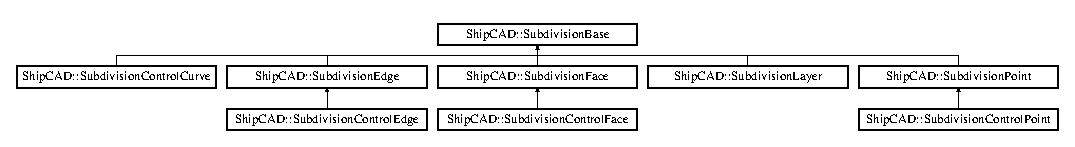
\includegraphics[height=2.045662cm]{classShipCAD_1_1SubdivisionBase}
\end{center}
\end{figure}
\subsection*{Public Member Functions}
\begin{DoxyCompactItemize}
\item 
\hyperlink{classShipCAD_1_1SubdivisionBase_ad424b99e73d138f565a152ed0ee648cb}{Subdivision\-Base} (\hyperlink{classShipCAD_1_1SubdivisionSurface}{Subdivision\-Surface} $\ast$owner)
\begin{DoxyCompactList}\small\item\em Constructor. \end{DoxyCompactList}\item 
virtual \hyperlink{classShipCAD_1_1SubdivisionBase_a12b4adebcd9fb52d4d82d9ff469e144d}{$\sim$\-Subdivision\-Base} ()
\item 
\hyperlink{classShipCAD_1_1SubdivisionSurface}{Subdivision\-Surface} $\ast$ \hyperlink{classShipCAD_1_1SubdivisionBase_a0b9a68b5c7e6a20cf52a465f2387ffba}{get\-Owner} ()
\begin{DoxyCompactList}\small\item\em get the owning surface \end{DoxyCompactList}\item 
virtual void \hyperlink{classShipCAD_1_1SubdivisionBase_a8f64480f79c9260facc2d27cd19a36ed}{set\-Owner} (\hyperlink{classShipCAD_1_1SubdivisionSurface}{Subdivision\-Surface} $\ast$newowner)
\begin{DoxyCompactList}\small\item\em set the owing surface \end{DoxyCompactList}\item 
virtual void \hyperlink{classShipCAD_1_1SubdivisionBase_a851bb7f1931f9dd6e53b6f9df7b5b352}{clear} ()=0
\begin{DoxyCompactList}\small\item\em reset this element to default values \end{DoxyCompactList}\item 
virtual void \hyperlink{classShipCAD_1_1SubdivisionBase_a7807e64ac8d2acc3da572e03cf0523b6}{dump} (std\-::ostream \&os, const char $\ast$prefix=\char`\"{}\char`\"{}) const 
\begin{DoxyCompactList}\small\item\em print out the element to a stream \end{DoxyCompactList}\end{DoxyCompactItemize}
\subsection*{Protected Member Functions}
\begin{DoxyCompactItemize}
\item 
void \hyperlink{classShipCAD_1_1SubdivisionBase_a024aa781bbf2e54b6fb088e33126998e}{priv\-\_\-dump} (std\-::ostream \&os, const char $\ast$prefix) const 
\begin{DoxyCompactList}\small\item\em dump the element to a stream \end{DoxyCompactList}\end{DoxyCompactItemize}
\subsection*{Protected Attributes}
\begin{DoxyCompactItemize}
\item 
\hyperlink{classShipCAD_1_1SubdivisionSurface}{Subdivision\-Surface} $\ast$ \hyperlink{classShipCAD_1_1SubdivisionBase_a164481259436bf18bc22a0626ab66c09}{\-\_\-owner}
\end{DoxyCompactItemize}
\subsection*{Properties}
\begin{DoxyCompactItemize}
\item 
\hyperlink{classShipCAD_1_1SubdivisionSurface}{Subdivision\-Surface} \hyperlink{classShipCAD_1_1SubdivisionBase_aa18f308b1a32286b3d29adcd6cb39ebf}{Owner}
\end{DoxyCompactItemize}


\subsection{Detailed Description}
the base class for all subdivision points, edges and faces 



Definition at line 46 of file subdivbase.\-h.



\subsection{Constructor \& Destructor Documentation}
\hypertarget{classShipCAD_1_1SubdivisionBase_ad424b99e73d138f565a152ed0ee648cb}{\index{Ship\-C\-A\-D\-::\-Subdivision\-Base@{Ship\-C\-A\-D\-::\-Subdivision\-Base}!Subdivision\-Base@{Subdivision\-Base}}
\index{Subdivision\-Base@{Subdivision\-Base}!ShipCAD::SubdivisionBase@{Ship\-C\-A\-D\-::\-Subdivision\-Base}}
\subsubsection[{Subdivision\-Base}]{\setlength{\rightskip}{0pt plus 5cm}Subdivision\-Base\-::\-Subdivision\-Base (
\begin{DoxyParamCaption}
\item[{{\bf Subdivision\-Surface} $\ast$}]{owner}
\end{DoxyParamCaption}
)\hspace{0.3cm}{\ttfamily [explicit]}}}\label{classShipCAD_1_1SubdivisionBase_ad424b99e73d138f565a152ed0ee648cb}


Constructor. 


\begin{DoxyParams}{Parameters}
{\em owner} & which surface this element belongs to \\
\hline
\end{DoxyParams}


Definition at line 40 of file subdivbase.\-cpp.

\hypertarget{classShipCAD_1_1SubdivisionBase_a12b4adebcd9fb52d4d82d9ff469e144d}{\index{Ship\-C\-A\-D\-::\-Subdivision\-Base@{Ship\-C\-A\-D\-::\-Subdivision\-Base}!$\sim$\-Subdivision\-Base@{$\sim$\-Subdivision\-Base}}
\index{$\sim$\-Subdivision\-Base@{$\sim$\-Subdivision\-Base}!ShipCAD::SubdivisionBase@{Ship\-C\-A\-D\-::\-Subdivision\-Base}}
\subsubsection[{$\sim$\-Subdivision\-Base}]{\setlength{\rightskip}{0pt plus 5cm}Subdivision\-Base\-::$\sim$\-Subdivision\-Base (
\begin{DoxyParamCaption}
{}
\end{DoxyParamCaption}
)\hspace{0.3cm}{\ttfamily [virtual]}}}\label{classShipCAD_1_1SubdivisionBase_a12b4adebcd9fb52d4d82d9ff469e144d}


Definition at line 46 of file subdivbase.\-cpp.



\subsection{Member Function Documentation}
\hypertarget{classShipCAD_1_1SubdivisionBase_a851bb7f1931f9dd6e53b6f9df7b5b352}{\index{Ship\-C\-A\-D\-::\-Subdivision\-Base@{Ship\-C\-A\-D\-::\-Subdivision\-Base}!clear@{clear}}
\index{clear@{clear}!ShipCAD::SubdivisionBase@{Ship\-C\-A\-D\-::\-Subdivision\-Base}}
\subsubsection[{clear}]{\setlength{\rightskip}{0pt plus 5cm}virtual void Ship\-C\-A\-D\-::\-Subdivision\-Base\-::clear (
\begin{DoxyParamCaption}
{}
\end{DoxyParamCaption}
)\hspace{0.3cm}{\ttfamily [pure virtual]}}}\label{classShipCAD_1_1SubdivisionBase_a851bb7f1931f9dd6e53b6f9df7b5b352}


reset this element to default values 



Implemented in \hyperlink{classShipCAD_1_1SubdivisionControlFace_ad168e31f0ef2537b3cd0f58b0c1c54e2}{Ship\-C\-A\-D\-::\-Subdivision\-Control\-Face}, \hyperlink{classShipCAD_1_1SubdivisionFace_a413ae7e76f559780c8a69e998974fb75}{Ship\-C\-A\-D\-::\-Subdivision\-Face}, \hyperlink{classShipCAD_1_1SubdivisionLayer_a7046d17ba87dd5ce7399f22ae327fc6e}{Ship\-C\-A\-D\-::\-Subdivision\-Layer}, \hyperlink{classShipCAD_1_1SubdivisionPoint_aef22d2b6cb48e57ce69652eeb7a69711}{Ship\-C\-A\-D\-::\-Subdivision\-Point}, \hyperlink{classShipCAD_1_1SubdivisionControlCurve_aa574f77f4abc5a8eef05e7cef7f8d8a2}{Ship\-C\-A\-D\-::\-Subdivision\-Control\-Curve}, and \hyperlink{classShipCAD_1_1SubdivisionEdge_a08358ac65c2d710855b8b93c64ce9d02}{Ship\-C\-A\-D\-::\-Subdivision\-Edge}.

\hypertarget{classShipCAD_1_1SubdivisionBase_a7807e64ac8d2acc3da572e03cf0523b6}{\index{Ship\-C\-A\-D\-::\-Subdivision\-Base@{Ship\-C\-A\-D\-::\-Subdivision\-Base}!dump@{dump}}
\index{dump@{dump}!ShipCAD::SubdivisionBase@{Ship\-C\-A\-D\-::\-Subdivision\-Base}}
\subsubsection[{dump}]{\setlength{\rightskip}{0pt plus 5cm}void Subdivision\-Base\-::dump (
\begin{DoxyParamCaption}
\item[{std\-::ostream \&}]{os, }
\item[{const char $\ast$}]{prefix = {\ttfamily \char`\"{}\char`\"{}}}
\end{DoxyParamCaption}
) const\hspace{0.3cm}{\ttfamily [virtual]}}}\label{classShipCAD_1_1SubdivisionBase_a7807e64ac8d2acc3da572e03cf0523b6}


print out the element to a stream 


\begin{DoxyParams}{Parameters}
{\em os} & the output stream \\
\hline
{\em prefix} & string to prefix on each line output \\
\hline
\end{DoxyParams}


Reimplemented in \hyperlink{classShipCAD_1_1SubdivisionControlFace_a947868fba3e9bb6c587847fb9245c9ff}{Ship\-C\-A\-D\-::\-Subdivision\-Control\-Face}, \hyperlink{classShipCAD_1_1SubdivisionControlPoint_a4a9d6e45291c27f19f0d76c9b9d19048}{Ship\-C\-A\-D\-::\-Subdivision\-Control\-Point}, \hyperlink{classShipCAD_1_1SubdivisionPoint_aed72cf5e8dc67e980010d195f3a376a3}{Ship\-C\-A\-D\-::\-Subdivision\-Point}, \hyperlink{classShipCAD_1_1SubdivisionFace_aa5bd261ae5fc0a1c7fe8cc5328b8477f}{Ship\-C\-A\-D\-::\-Subdivision\-Face}, \hyperlink{classShipCAD_1_1SubdivisionControlEdge_abdfa96ff05eff404214a92d38d7eb715}{Ship\-C\-A\-D\-::\-Subdivision\-Control\-Edge}, \hyperlink{classShipCAD_1_1SubdivisionLayer_ab41e005f720a2bba4b2efa74bfd5943e}{Ship\-C\-A\-D\-::\-Subdivision\-Layer}, \hyperlink{classShipCAD_1_1SubdivisionControlCurve_a30e8d074583a386be2ab6343cb5f8502}{Ship\-C\-A\-D\-::\-Subdivision\-Control\-Curve}, and \hyperlink{classShipCAD_1_1SubdivisionEdge_a14cc58877644ebd7b7ebffbdf8ef87f7}{Ship\-C\-A\-D\-::\-Subdivision\-Edge}.



Definition at line 51 of file subdivbase.\-cpp.

\hypertarget{classShipCAD_1_1SubdivisionBase_a0b9a68b5c7e6a20cf52a465f2387ffba}{\index{Ship\-C\-A\-D\-::\-Subdivision\-Base@{Ship\-C\-A\-D\-::\-Subdivision\-Base}!get\-Owner@{get\-Owner}}
\index{get\-Owner@{get\-Owner}!ShipCAD::SubdivisionBase@{Ship\-C\-A\-D\-::\-Subdivision\-Base}}
\subsubsection[{get\-Owner}]{\setlength{\rightskip}{0pt plus 5cm}{\bf Subdivision\-Surface}$\ast$ Ship\-C\-A\-D\-::\-Subdivision\-Base\-::get\-Owner (
\begin{DoxyParamCaption}
{}
\end{DoxyParamCaption}
)\hspace{0.3cm}{\ttfamily [inline]}}}\label{classShipCAD_1_1SubdivisionBase_a0b9a68b5c7e6a20cf52a465f2387ffba}


get the owning surface 

\begin{DoxyReturn}{Returns}
the owning surface 
\end{DoxyReturn}


Definition at line 64 of file subdivbase.\-h.

\hypertarget{classShipCAD_1_1SubdivisionBase_a024aa781bbf2e54b6fb088e33126998e}{\index{Ship\-C\-A\-D\-::\-Subdivision\-Base@{Ship\-C\-A\-D\-::\-Subdivision\-Base}!priv\-\_\-dump@{priv\-\_\-dump}}
\index{priv\-\_\-dump@{priv\-\_\-dump}!ShipCAD::SubdivisionBase@{Ship\-C\-A\-D\-::\-Subdivision\-Base}}
\subsubsection[{priv\-\_\-dump}]{\setlength{\rightskip}{0pt plus 5cm}void Subdivision\-Base\-::priv\-\_\-dump (
\begin{DoxyParamCaption}
\item[{std\-::ostream \&}]{os, }
\item[{const char $\ast$}]{prefix}
\end{DoxyParamCaption}
) const\hspace{0.3cm}{\ttfamily [protected]}}}\label{classShipCAD_1_1SubdivisionBase_a024aa781bbf2e54b6fb088e33126998e}


dump the element to a stream 


\begin{DoxyParams}{Parameters}
{\em os} & the output stream \\
\hline
{\em prefix} & string to prefix on each line output \\
\hline
\end{DoxyParams}


Definition at line 57 of file subdivbase.\-cpp.

\hypertarget{classShipCAD_1_1SubdivisionBase_a8f64480f79c9260facc2d27cd19a36ed}{\index{Ship\-C\-A\-D\-::\-Subdivision\-Base@{Ship\-C\-A\-D\-::\-Subdivision\-Base}!set\-Owner@{set\-Owner}}
\index{set\-Owner@{set\-Owner}!ShipCAD::SubdivisionBase@{Ship\-C\-A\-D\-::\-Subdivision\-Base}}
\subsubsection[{set\-Owner}]{\setlength{\rightskip}{0pt plus 5cm}virtual void Ship\-C\-A\-D\-::\-Subdivision\-Base\-::set\-Owner (
\begin{DoxyParamCaption}
\item[{{\bf Subdivision\-Surface} $\ast$}]{newowner}
\end{DoxyParamCaption}
)\hspace{0.3cm}{\ttfamily [inline]}, {\ttfamily [virtual]}}}\label{classShipCAD_1_1SubdivisionBase_a8f64480f79c9260facc2d27cd19a36ed}


set the owing surface 


\begin{DoxyParams}{Parameters}
{\em newowner} & the owning surface \\
\hline
\end{DoxyParams}


Definition at line 69 of file subdivbase.\-h.



\subsection{Member Data Documentation}
\hypertarget{classShipCAD_1_1SubdivisionBase_a164481259436bf18bc22a0626ab66c09}{\index{Ship\-C\-A\-D\-::\-Subdivision\-Base@{Ship\-C\-A\-D\-::\-Subdivision\-Base}!\-\_\-owner@{\-\_\-owner}}
\index{\-\_\-owner@{\-\_\-owner}!ShipCAD::SubdivisionBase@{Ship\-C\-A\-D\-::\-Subdivision\-Base}}
\subsubsection[{\-\_\-owner}]{\setlength{\rightskip}{0pt plus 5cm}{\bf Subdivision\-Surface}$\ast$ Ship\-C\-A\-D\-::\-Subdivision\-Base\-::\-\_\-owner\hspace{0.3cm}{\ttfamily [protected]}}}\label{classShipCAD_1_1SubdivisionBase_a164481259436bf18bc22a0626ab66c09}
the owning surface 

Definition at line 94 of file subdivbase.\-h.



\subsection{Property Documentation}
\hypertarget{classShipCAD_1_1SubdivisionBase_aa18f308b1a32286b3d29adcd6cb39ebf}{\index{Ship\-C\-A\-D\-::\-Subdivision\-Base@{Ship\-C\-A\-D\-::\-Subdivision\-Base}!Owner@{Owner}}
\index{Owner@{Owner}!ShipCAD::SubdivisionBase@{Ship\-C\-A\-D\-::\-Subdivision\-Base}}
\subsubsection[{Owner}]{\setlength{\rightskip}{0pt plus 5cm}{\bf Subdivision\-Surface} Ship\-C\-A\-D\-::\-Subdivision\-Base\-::\-Owner\hspace{0.3cm}{\ttfamily [read]}}}\label{classShipCAD_1_1SubdivisionBase_aa18f308b1a32286b3d29adcd6cb39ebf}


Definition at line 49 of file subdivbase.\-h.



The documentation for this class was generated from the following files\-:\begin{DoxyCompactItemize}
\item 
Ship\-C\-A\-Dlib/\hyperlink{subdivbase_8h}{subdivbase.\-h}\item 
Ship\-C\-A\-Dlib/\hyperlink{subdivbase_8cpp}{subdivbase.\-cpp}\end{DoxyCompactItemize}

\hypertarget{classShipCAD_1_1SubdivisionControlCurve}{\section{Ship\-C\-A\-D\-:\-:Subdivision\-Control\-Curve Class Reference}
\label{classShipCAD_1_1SubdivisionControlCurve}\index{Ship\-C\-A\-D\-::\-Subdivision\-Control\-Curve@{Ship\-C\-A\-D\-::\-Subdivision\-Control\-Curve}}
}


{\ttfamily \#include $<$subdivcontrolcurve.\-h$>$}

Inheritance diagram for Ship\-C\-A\-D\-:\-:Subdivision\-Control\-Curve\-:\begin{figure}[H]
\begin{center}
\leavevmode
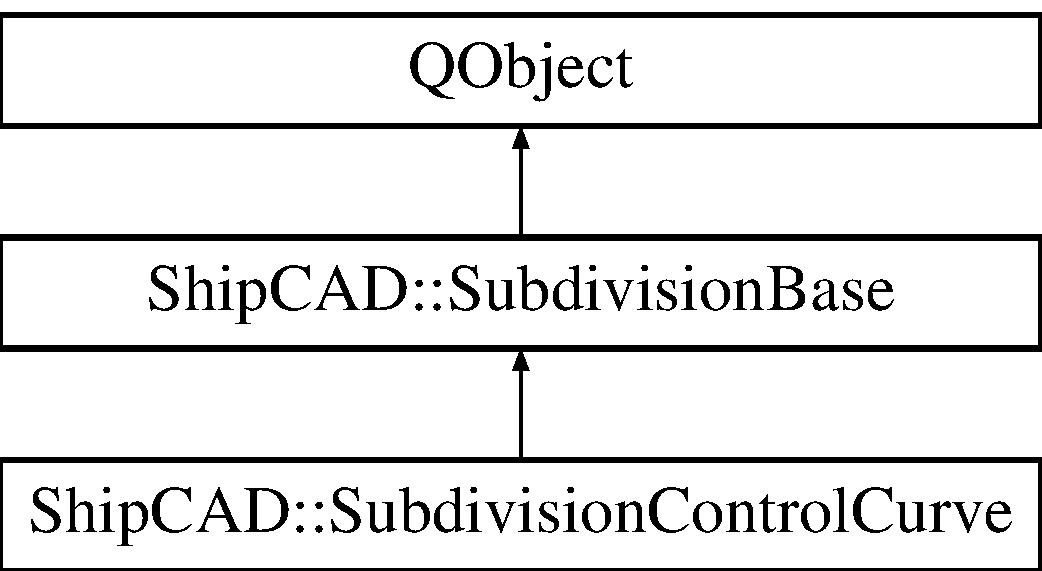
\includegraphics[height=3.000000cm]{classShipCAD_1_1SubdivisionControlCurve}
\end{center}
\end{figure}
\subsection*{Public Member Functions}
\begin{DoxyCompactItemize}
\item 
\hyperlink{classShipCAD_1_1SubdivisionControlCurve_adfdaa3dcd794901f3c1277223eab22f9}{Subdivision\-Control\-Curve} (\hyperlink{classShipCAD_1_1SubdivisionSurface}{Subdivision\-Surface} $\ast$owner)
\item 
virtual \hyperlink{classShipCAD_1_1SubdivisionControlCurve_a5b3d3e0b700afd7a7a1da0e5dfafdfb9}{$\sim$\-Subdivision\-Control\-Curve} ()
\item 
void \hyperlink{classShipCAD_1_1SubdivisionControlCurve_a078fc8820a6c0e37c475eec1897b13dd}{replace\-Vertex\-Point} (\hyperlink{classShipCAD_1_1SubdivisionPoint}{Subdivision\-Point} $\ast$oldpt, \hyperlink{classShipCAD_1_1SubdivisionPoint}{Subdivision\-Point} $\ast$newpt)
\item 
void \hyperlink{classShipCAD_1_1SubdivisionControlCurve_a0764f5d7697b76ac928a121d224733f5}{insert\-Edge\-Point} (\hyperlink{classShipCAD_1_1SubdivisionPoint}{Subdivision\-Point} $\ast$p1, \hyperlink{classShipCAD_1_1SubdivisionPoint}{Subdivision\-Point} $\ast$p2, \hyperlink{classShipCAD_1_1SubdivisionPoint}{Subdivision\-Point} $\ast$newpt)
\item 
void \hyperlink{classShipCAD_1_1SubdivisionControlCurve_abfed48331919c4d2a2bfc6363b28ebb4}{delete\-Edge} (\hyperlink{classShipCAD_1_1SubdivisionControlEdge}{Subdivision\-Control\-Edge} $\ast$edge)
\item 
void \hyperlink{classShipCAD_1_1SubdivisionControlCurve_a9469b178a88269d0f9ee3b17d5f15272}{insert\-Control\-Point} (\hyperlink{classShipCAD_1_1SubdivisionControlPoint}{Subdivision\-Control\-Point} $\ast$p1, \hyperlink{classShipCAD_1_1SubdivisionControlPoint}{Subdivision\-Control\-Point} $\ast$p2, \hyperlink{classShipCAD_1_1SubdivisionControlPoint}{Subdivision\-Control\-Point} $\ast$newpt)
\item 
void \hyperlink{classShipCAD_1_1SubdivisionControlCurve_a1155b0abe401a7128369a589b6e6ac9c}{add\-Point} (\hyperlink{classShipCAD_1_1SubdivisionControlPoint}{Subdivision\-Control\-Point} $\ast$p)
\item 
virtual void \hyperlink{classShipCAD_1_1SubdivisionControlCurve_aa574f77f4abc5a8eef05e7cef7f8d8a2}{clear} ()
\begin{DoxyCompactList}\small\item\em reset this element to default values \end{DoxyCompactList}\item 
void \hyperlink{classShipCAD_1_1SubdivisionControlCurve_a34e280e9ba6e6705577d1afd229e9f20}{reset\-Div\-Points} ()
\item 
bool \hyperlink{classShipCAD_1_1SubdivisionControlCurve_a8b3c57aba1c16b77b902daacd7b88d0c}{is\-Selected} ()
\item 
bool \hyperlink{classShipCAD_1_1SubdivisionControlCurve_a36bcf74cf20d7f1ae888f25f774b040d}{is\-Visible} ()
\item 
bool \hyperlink{classShipCAD_1_1SubdivisionControlCurve_a6d0039b0dac74ed558bfb684fb4b4497}{is\-Build} ()
\item 
Q\-Color \hyperlink{classShipCAD_1_1SubdivisionControlCurve_a1dd7d33fd574c3cfdd53ccbb13abb695}{get\-Color} ()
\item 
size\-\_\-t \hyperlink{classShipCAD_1_1SubdivisionControlCurve_aaa9d504f115655dbb930493d96b9db62}{number\-Of\-Control\-Points} ()
\item 
size\-\_\-t \hyperlink{classShipCAD_1_1SubdivisionControlCurve_a7b68fcef6035edcb10fedc996d10272f}{number\-Of\-Subdiv\-Points} ()
\item 
\hyperlink{classShipCAD_1_1SubdivisionControlPoint}{Subdivision\-Control\-Point} $\ast$ \hyperlink{classShipCAD_1_1SubdivisionControlCurve_a0331fade870dd4856c070e2f487882b5}{get\-Control\-Point} (size\-\_\-t index)
\item 
\hyperlink{classShipCAD_1_1SubdivisionPoint}{Subdivision\-Point} $\ast$ \hyperlink{classShipCAD_1_1SubdivisionControlCurve_a52b12b58d524baba317ab6504e80018f}{get\-Subdiv\-Point} (size\-\_\-t index)
\item 
void \hyperlink{classShipCAD_1_1SubdivisionControlCurve_ac536de424624a4ae312029fe643f4b61}{set\-Visible} (bool val)
\item 
void \hyperlink{classShipCAD_1_1SubdivisionControlCurve_afb98b225e0dc255272a69e96c14eedb7}{set\-Build} (bool val)
\item 
void \hyperlink{classShipCAD_1_1SubdivisionControlCurve_abaf7f7cfec21eedacf55b1654f3e7f2f}{set\-Selected} (bool val)
\item 
\hyperlink{classShipCAD_1_1Spline}{Spline} $\ast$ \hyperlink{classShipCAD_1_1SubdivisionControlCurve_a83a97a77d42df146d45d3751d8973f02}{get\-Spline} ()
\item 
void \hyperlink{classShipCAD_1_1SubdivisionControlCurve_ad2a7118ea074ce1b7f61586f08039d2a}{load\-Binary} (\hyperlink{classShipCAD_1_1FileBuffer}{File\-Buffer} \&source)
\item 
void \hyperlink{classShipCAD_1_1SubdivisionControlCurve_a3ef4c7ce3e2d9a2fe4f90ebf35ffc033}{save\-Binary} (\hyperlink{classShipCAD_1_1FileBuffer}{File\-Buffer} \&destiniation)
\item 
void \hyperlink{classShipCAD_1_1SubdivisionControlCurve_a22726dc4edf385c5b4b5fead84d4c3de}{save\-To\-D\-X\-F} (std\-::vector$<$ Q\-String $>$ \&strings)
\item 
virtual void \hyperlink{classShipCAD_1_1SubdivisionControlCurve_a4d7d8e87dc582529e763039ffe593360}{draw} (\hyperlink{classShipCAD_1_1Viewport}{Viewport} \&vp, \hyperlink{classShipCAD_1_1LineShader}{Line\-Shader} $\ast$lineshader)
\item 
virtual void \hyperlink{classShipCAD_1_1SubdivisionControlCurve_a30e8d074583a386be2ab6343cb5f8502}{dump} (std\-::ostream \&os, const char $\ast$prefix=\char`\"{}\char`\"{}) const 
\begin{DoxyCompactList}\small\item\em print out the element to a stream \end{DoxyCompactList}\end{DoxyCompactItemize}
\subsection*{Static Public Member Functions}
\begin{DoxyCompactItemize}
\item 
static \hyperlink{classShipCAD_1_1SubdivisionControlCurve}{Subdivision\-Control\-Curve} $\ast$ \hyperlink{classShipCAD_1_1SubdivisionControlCurve_a21d9226cc2fd7efcaf6f1067912a0b34}{construct} (\hyperlink{classShipCAD_1_1SubdivisionSurface}{Subdivision\-Surface} $\ast$owner)
\end{DoxyCompactItemize}
\subsection*{Protected Member Functions}
\begin{DoxyCompactItemize}
\item 
void \hyperlink{classShipCAD_1_1SubdivisionControlCurve_a48fbb761e8c85120ba7f6876d873e898}{priv\-\_\-dump} (std\-::ostream \&os, const char $\ast$prefix) const 
\end{DoxyCompactItemize}
\subsection*{Protected Attributes}
\begin{DoxyCompactItemize}
\item 
bool \hyperlink{classShipCAD_1_1SubdivisionControlCurve_a1e4dd9968f46becb714e44709d0da418}{\-\_\-build}
\item 
std\-::vector\\*
$<$ \hyperlink{classShipCAD_1_1SubdivisionControlPoint}{Subdivision\-Control\-Point} $\ast$ $>$ \hyperlink{classShipCAD_1_1SubdivisionControlCurve_ac54ea0783b3f8f2aa65d49fe489f1b4f}{\-\_\-points}
\item 
std\-::vector$<$ \hyperlink{classShipCAD_1_1SubdivisionPoint}{Subdivision\-Point} $\ast$ $>$ \hyperlink{classShipCAD_1_1SubdivisionControlCurve_af91dbc96b703fe618567326cca21d82c}{\-\_\-div\-\_\-points}
\item 
\hyperlink{classShipCAD_1_1Spline}{Spline} $\ast$ \hyperlink{classShipCAD_1_1SubdivisionControlCurve_a115a5b67ed81a3012ccb02a25b3d2c24}{\-\_\-curve}
\end{DoxyCompactItemize}
\subsection*{Additional Inherited Members}


\subsection{Detailed Description}


Definition at line 55 of file subdivcontrolcurve.\-h.



\subsection{Constructor \& Destructor Documentation}
\hypertarget{classShipCAD_1_1SubdivisionControlCurve_adfdaa3dcd794901f3c1277223eab22f9}{\index{Ship\-C\-A\-D\-::\-Subdivision\-Control\-Curve@{Ship\-C\-A\-D\-::\-Subdivision\-Control\-Curve}!Subdivision\-Control\-Curve@{Subdivision\-Control\-Curve}}
\index{Subdivision\-Control\-Curve@{Subdivision\-Control\-Curve}!ShipCAD::SubdivisionControlCurve@{Ship\-C\-A\-D\-::\-Subdivision\-Control\-Curve}}
\subsubsection[{Subdivision\-Control\-Curve}]{\setlength{\rightskip}{0pt plus 5cm}Subdivision\-Control\-Curve\-::\-Subdivision\-Control\-Curve (
\begin{DoxyParamCaption}
\item[{{\bf Subdivision\-Surface} $\ast$}]{owner}
\end{DoxyParamCaption}
)\hspace{0.3cm}{\ttfamily [explicit]}}}\label{classShipCAD_1_1SubdivisionControlCurve_adfdaa3dcd794901f3c1277223eab22f9}


Definition at line 57 of file subdivcontrolcurve.\-cpp.

\hypertarget{classShipCAD_1_1SubdivisionControlCurve_a5b3d3e0b700afd7a7a1da0e5dfafdfb9}{\index{Ship\-C\-A\-D\-::\-Subdivision\-Control\-Curve@{Ship\-C\-A\-D\-::\-Subdivision\-Control\-Curve}!$\sim$\-Subdivision\-Control\-Curve@{$\sim$\-Subdivision\-Control\-Curve}}
\index{$\sim$\-Subdivision\-Control\-Curve@{$\sim$\-Subdivision\-Control\-Curve}!ShipCAD::SubdivisionControlCurve@{Ship\-C\-A\-D\-::\-Subdivision\-Control\-Curve}}
\subsubsection[{$\sim$\-Subdivision\-Control\-Curve}]{\setlength{\rightskip}{0pt plus 5cm}Subdivision\-Control\-Curve\-::$\sim$\-Subdivision\-Control\-Curve (
\begin{DoxyParamCaption}
{}
\end{DoxyParamCaption}
)\hspace{0.3cm}{\ttfamily [virtual]}}}\label{classShipCAD_1_1SubdivisionControlCurve_a5b3d3e0b700afd7a7a1da0e5dfafdfb9}


Definition at line 63 of file subdivcontrolcurve.\-cpp.



\subsection{Member Function Documentation}
\hypertarget{classShipCAD_1_1SubdivisionControlCurve_a1155b0abe401a7128369a589b6e6ac9c}{\index{Ship\-C\-A\-D\-::\-Subdivision\-Control\-Curve@{Ship\-C\-A\-D\-::\-Subdivision\-Control\-Curve}!add\-Point@{add\-Point}}
\index{add\-Point@{add\-Point}!ShipCAD::SubdivisionControlCurve@{Ship\-C\-A\-D\-::\-Subdivision\-Control\-Curve}}
\subsubsection[{add\-Point}]{\setlength{\rightskip}{0pt plus 5cm}void Subdivision\-Control\-Curve\-::add\-Point (
\begin{DoxyParamCaption}
\item[{{\bf Subdivision\-Control\-Point} $\ast$}]{p}
\end{DoxyParamCaption}
)}}\label{classShipCAD_1_1SubdivisionControlCurve_a1155b0abe401a7128369a589b6e6ac9c}


Definition at line 96 of file subdivcontrolcurve.\-cpp.

\hypertarget{classShipCAD_1_1SubdivisionControlCurve_aa574f77f4abc5a8eef05e7cef7f8d8a2}{\index{Ship\-C\-A\-D\-::\-Subdivision\-Control\-Curve@{Ship\-C\-A\-D\-::\-Subdivision\-Control\-Curve}!clear@{clear}}
\index{clear@{clear}!ShipCAD::SubdivisionControlCurve@{Ship\-C\-A\-D\-::\-Subdivision\-Control\-Curve}}
\subsubsection[{clear}]{\setlength{\rightskip}{0pt plus 5cm}void Subdivision\-Control\-Curve\-::clear (
\begin{DoxyParamCaption}
{}
\end{DoxyParamCaption}
)\hspace{0.3cm}{\ttfamily [virtual]}}}\label{classShipCAD_1_1SubdivisionControlCurve_aa574f77f4abc5a8eef05e7cef7f8d8a2}


reset this element to default values 



Implements \hyperlink{classShipCAD_1_1SubdivisionBase_a851bb7f1931f9dd6e53b6f9df7b5b352}{Ship\-C\-A\-D\-::\-Subdivision\-Base}.



Definition at line 141 of file subdivcontrolcurve.\-cpp.

\hypertarget{classShipCAD_1_1SubdivisionControlCurve_a21d9226cc2fd7efcaf6f1067912a0b34}{\index{Ship\-C\-A\-D\-::\-Subdivision\-Control\-Curve@{Ship\-C\-A\-D\-::\-Subdivision\-Control\-Curve}!construct@{construct}}
\index{construct@{construct}!ShipCAD::SubdivisionControlCurve@{Ship\-C\-A\-D\-::\-Subdivision\-Control\-Curve}}
\subsubsection[{construct}]{\setlength{\rightskip}{0pt plus 5cm}{\bf Subdivision\-Control\-Curve} $\ast$ Subdivision\-Control\-Curve\-::construct (
\begin{DoxyParamCaption}
\item[{{\bf Subdivision\-Surface} $\ast$}]{owner}
\end{DoxyParamCaption}
)\hspace{0.3cm}{\ttfamily [static]}}}\label{classShipCAD_1_1SubdivisionControlCurve_a21d9226cc2fd7efcaf6f1067912a0b34}


Definition at line 49 of file subdivcontrolcurve.\-cpp.

\hypertarget{classShipCAD_1_1SubdivisionControlCurve_abfed48331919c4d2a2bfc6363b28ebb4}{\index{Ship\-C\-A\-D\-::\-Subdivision\-Control\-Curve@{Ship\-C\-A\-D\-::\-Subdivision\-Control\-Curve}!delete\-Edge@{delete\-Edge}}
\index{delete\-Edge@{delete\-Edge}!ShipCAD::SubdivisionControlCurve@{Ship\-C\-A\-D\-::\-Subdivision\-Control\-Curve}}
\subsubsection[{delete\-Edge}]{\setlength{\rightskip}{0pt plus 5cm}void Subdivision\-Control\-Curve\-::delete\-Edge (
\begin{DoxyParamCaption}
\item[{{\bf Subdivision\-Control\-Edge} $\ast$}]{edge}
\end{DoxyParamCaption}
)}}\label{classShipCAD_1_1SubdivisionControlCurve_abfed48331919c4d2a2bfc6363b28ebb4}


Definition at line 149 of file subdivcontrolcurve.\-cpp.

\hypertarget{classShipCAD_1_1SubdivisionControlCurve_a4d7d8e87dc582529e763039ffe593360}{\index{Ship\-C\-A\-D\-::\-Subdivision\-Control\-Curve@{Ship\-C\-A\-D\-::\-Subdivision\-Control\-Curve}!draw@{draw}}
\index{draw@{draw}!ShipCAD::SubdivisionControlCurve@{Ship\-C\-A\-D\-::\-Subdivision\-Control\-Curve}}
\subsubsection[{draw}]{\setlength{\rightskip}{0pt plus 5cm}void Subdivision\-Control\-Curve\-::draw (
\begin{DoxyParamCaption}
\item[{{\bf Viewport} \&}]{vp, }
\item[{{\bf Line\-Shader} $\ast$}]{lineshader}
\end{DoxyParamCaption}
)\hspace{0.3cm}{\ttfamily [virtual]}}}\label{classShipCAD_1_1SubdivisionControlCurve_a4d7d8e87dc582529e763039ffe593360}


Definition at line 222 of file subdivcontrolcurve.\-cpp.

\hypertarget{classShipCAD_1_1SubdivisionControlCurve_a30e8d074583a386be2ab6343cb5f8502}{\index{Ship\-C\-A\-D\-::\-Subdivision\-Control\-Curve@{Ship\-C\-A\-D\-::\-Subdivision\-Control\-Curve}!dump@{dump}}
\index{dump@{dump}!ShipCAD::SubdivisionControlCurve@{Ship\-C\-A\-D\-::\-Subdivision\-Control\-Curve}}
\subsubsection[{dump}]{\setlength{\rightskip}{0pt plus 5cm}void Subdivision\-Control\-Curve\-::dump (
\begin{DoxyParamCaption}
\item[{std\-::ostream \&}]{os, }
\item[{const char $\ast$}]{prefix = {\ttfamily \char`\"{}\char`\"{}}}
\end{DoxyParamCaption}
) const\hspace{0.3cm}{\ttfamily [virtual]}}}\label{classShipCAD_1_1SubdivisionControlCurve_a30e8d074583a386be2ab6343cb5f8502}


print out the element to a stream 


\begin{DoxyParams}{Parameters}
{\em os} & the output stream \\
\hline
{\em prefix} & string to prefix on each line output \\
\hline
\end{DoxyParams}


Reimplemented from \hyperlink{classShipCAD_1_1SubdivisionBase_a7807e64ac8d2acc3da572e03cf0523b6}{Ship\-C\-A\-D\-::\-Subdivision\-Base}.



Definition at line 402 of file subdivcontrolcurve.\-cpp.

\hypertarget{classShipCAD_1_1SubdivisionControlCurve_a1dd7d33fd574c3cfdd53ccbb13abb695}{\index{Ship\-C\-A\-D\-::\-Subdivision\-Control\-Curve@{Ship\-C\-A\-D\-::\-Subdivision\-Control\-Curve}!get\-Color@{get\-Color}}
\index{get\-Color@{get\-Color}!ShipCAD::SubdivisionControlCurve@{Ship\-C\-A\-D\-::\-Subdivision\-Control\-Curve}}
\subsubsection[{get\-Color}]{\setlength{\rightskip}{0pt plus 5cm}Q\-Color Subdivision\-Control\-Curve\-::get\-Color (
\begin{DoxyParamCaption}
{}
\end{DoxyParamCaption}
)}}\label{classShipCAD_1_1SubdivisionControlCurve_a1dd7d33fd574c3cfdd53ccbb13abb695}


Definition at line 110 of file subdivcontrolcurve.\-cpp.

\hypertarget{classShipCAD_1_1SubdivisionControlCurve_a0331fade870dd4856c070e2f487882b5}{\index{Ship\-C\-A\-D\-::\-Subdivision\-Control\-Curve@{Ship\-C\-A\-D\-::\-Subdivision\-Control\-Curve}!get\-Control\-Point@{get\-Control\-Point}}
\index{get\-Control\-Point@{get\-Control\-Point}!ShipCAD::SubdivisionControlCurve@{Ship\-C\-A\-D\-::\-Subdivision\-Control\-Curve}}
\subsubsection[{get\-Control\-Point}]{\setlength{\rightskip}{0pt plus 5cm}{\bf Subdivision\-Control\-Point} $\ast$ Subdivision\-Control\-Curve\-::get\-Control\-Point (
\begin{DoxyParamCaption}
\item[{size\-\_\-t}]{index}
\end{DoxyParamCaption}
)}}\label{classShipCAD_1_1SubdivisionControlCurve_a0331fade870dd4856c070e2f487882b5}


Definition at line 127 of file subdivcontrolcurve.\-cpp.

\hypertarget{classShipCAD_1_1SubdivisionControlCurve_a83a97a77d42df146d45d3751d8973f02}{\index{Ship\-C\-A\-D\-::\-Subdivision\-Control\-Curve@{Ship\-C\-A\-D\-::\-Subdivision\-Control\-Curve}!get\-Spline@{get\-Spline}}
\index{get\-Spline@{get\-Spline}!ShipCAD::SubdivisionControlCurve@{Ship\-C\-A\-D\-::\-Subdivision\-Control\-Curve}}
\subsubsection[{get\-Spline}]{\setlength{\rightskip}{0pt plus 5cm}{\bf Spline}$\ast$ Ship\-C\-A\-D\-::\-Subdivision\-Control\-Curve\-::get\-Spline (
\begin{DoxyParamCaption}
{}
\end{DoxyParamCaption}
)\hspace{0.3cm}{\ttfamily [inline]}}}\label{classShipCAD_1_1SubdivisionControlCurve_a83a97a77d42df146d45d3751d8973f02}


Definition at line 87 of file subdivcontrolcurve.\-h.

\hypertarget{classShipCAD_1_1SubdivisionControlCurve_a52b12b58d524baba317ab6504e80018f}{\index{Ship\-C\-A\-D\-::\-Subdivision\-Control\-Curve@{Ship\-C\-A\-D\-::\-Subdivision\-Control\-Curve}!get\-Subdiv\-Point@{get\-Subdiv\-Point}}
\index{get\-Subdiv\-Point@{get\-Subdiv\-Point}!ShipCAD::SubdivisionControlCurve@{Ship\-C\-A\-D\-::\-Subdivision\-Control\-Curve}}
\subsubsection[{get\-Subdiv\-Point}]{\setlength{\rightskip}{0pt plus 5cm}{\bf Subdivision\-Point} $\ast$ Subdivision\-Control\-Curve\-::get\-Subdiv\-Point (
\begin{DoxyParamCaption}
\item[{size\-\_\-t}]{index}
\end{DoxyParamCaption}
)}}\label{classShipCAD_1_1SubdivisionControlCurve_a52b12b58d524baba317ab6504e80018f}


Definition at line 134 of file subdivcontrolcurve.\-cpp.

\hypertarget{classShipCAD_1_1SubdivisionControlCurve_a9469b178a88269d0f9ee3b17d5f15272}{\index{Ship\-C\-A\-D\-::\-Subdivision\-Control\-Curve@{Ship\-C\-A\-D\-::\-Subdivision\-Control\-Curve}!insert\-Control\-Point@{insert\-Control\-Point}}
\index{insert\-Control\-Point@{insert\-Control\-Point}!ShipCAD::SubdivisionControlCurve@{Ship\-C\-A\-D\-::\-Subdivision\-Control\-Curve}}
\subsubsection[{insert\-Control\-Point}]{\setlength{\rightskip}{0pt plus 5cm}void Subdivision\-Control\-Curve\-::insert\-Control\-Point (
\begin{DoxyParamCaption}
\item[{{\bf Subdivision\-Control\-Point} $\ast$}]{p1, }
\item[{{\bf Subdivision\-Control\-Point} $\ast$}]{p2, }
\item[{{\bf Subdivision\-Control\-Point} $\ast$}]{newpt}
\end{DoxyParamCaption}
)}}\label{classShipCAD_1_1SubdivisionControlCurve_a9469b178a88269d0f9ee3b17d5f15272}


Definition at line 326 of file subdivcontrolcurve.\-cpp.

\hypertarget{classShipCAD_1_1SubdivisionControlCurve_a0764f5d7697b76ac928a121d224733f5}{\index{Ship\-C\-A\-D\-::\-Subdivision\-Control\-Curve@{Ship\-C\-A\-D\-::\-Subdivision\-Control\-Curve}!insert\-Edge\-Point@{insert\-Edge\-Point}}
\index{insert\-Edge\-Point@{insert\-Edge\-Point}!ShipCAD::SubdivisionControlCurve@{Ship\-C\-A\-D\-::\-Subdivision\-Control\-Curve}}
\subsubsection[{insert\-Edge\-Point}]{\setlength{\rightskip}{0pt plus 5cm}void Subdivision\-Control\-Curve\-::insert\-Edge\-Point (
\begin{DoxyParamCaption}
\item[{{\bf Subdivision\-Point} $\ast$}]{p1, }
\item[{{\bf Subdivision\-Point} $\ast$}]{p2, }
\item[{{\bf Subdivision\-Point} $\ast$}]{newpt}
\end{DoxyParamCaption}
)}}\label{classShipCAD_1_1SubdivisionControlCurve_a0764f5d7697b76ac928a121d224733f5}


Definition at line 338 of file subdivcontrolcurve.\-cpp.

\hypertarget{classShipCAD_1_1SubdivisionControlCurve_a6d0039b0dac74ed558bfb684fb4b4497}{\index{Ship\-C\-A\-D\-::\-Subdivision\-Control\-Curve@{Ship\-C\-A\-D\-::\-Subdivision\-Control\-Curve}!is\-Build@{is\-Build}}
\index{is\-Build@{is\-Build}!ShipCAD::SubdivisionControlCurve@{Ship\-C\-A\-D\-::\-Subdivision\-Control\-Curve}}
\subsubsection[{is\-Build}]{\setlength{\rightskip}{0pt plus 5cm}bool Ship\-C\-A\-D\-::\-Subdivision\-Control\-Curve\-::is\-Build (
\begin{DoxyParamCaption}
{}
\end{DoxyParamCaption}
)\hspace{0.3cm}{\ttfamily [inline]}}}\label{classShipCAD_1_1SubdivisionControlCurve_a6d0039b0dac74ed558bfb684fb4b4497}


Definition at line 78 of file subdivcontrolcurve.\-h.

\hypertarget{classShipCAD_1_1SubdivisionControlCurve_a8b3c57aba1c16b77b902daacd7b88d0c}{\index{Ship\-C\-A\-D\-::\-Subdivision\-Control\-Curve@{Ship\-C\-A\-D\-::\-Subdivision\-Control\-Curve}!is\-Selected@{is\-Selected}}
\index{is\-Selected@{is\-Selected}!ShipCAD::SubdivisionControlCurve@{Ship\-C\-A\-D\-::\-Subdivision\-Control\-Curve}}
\subsubsection[{is\-Selected}]{\setlength{\rightskip}{0pt plus 5cm}bool Subdivision\-Control\-Curve\-::is\-Selected (
\begin{DoxyParamCaption}
{}
\end{DoxyParamCaption}
)}}\label{classShipCAD_1_1SubdivisionControlCurve_a8b3c57aba1c16b77b902daacd7b88d0c}


Definition at line 117 of file subdivcontrolcurve.\-cpp.

\hypertarget{classShipCAD_1_1SubdivisionControlCurve_a36bcf74cf20d7f1ae888f25f774b040d}{\index{Ship\-C\-A\-D\-::\-Subdivision\-Control\-Curve@{Ship\-C\-A\-D\-::\-Subdivision\-Control\-Curve}!is\-Visible@{is\-Visible}}
\index{is\-Visible@{is\-Visible}!ShipCAD::SubdivisionControlCurve@{Ship\-C\-A\-D\-::\-Subdivision\-Control\-Curve}}
\subsubsection[{is\-Visible}]{\setlength{\rightskip}{0pt plus 5cm}bool Subdivision\-Control\-Curve\-::is\-Visible (
\begin{DoxyParamCaption}
{}
\end{DoxyParamCaption}
)}}\label{classShipCAD_1_1SubdivisionControlCurve_a36bcf74cf20d7f1ae888f25f774b040d}


Definition at line 122 of file subdivcontrolcurve.\-cpp.

\hypertarget{classShipCAD_1_1SubdivisionControlCurve_ad2a7118ea074ce1b7f61586f08039d2a}{\index{Ship\-C\-A\-D\-::\-Subdivision\-Control\-Curve@{Ship\-C\-A\-D\-::\-Subdivision\-Control\-Curve}!load\-Binary@{load\-Binary}}
\index{load\-Binary@{load\-Binary}!ShipCAD::SubdivisionControlCurve@{Ship\-C\-A\-D\-::\-Subdivision\-Control\-Curve}}
\subsubsection[{load\-Binary}]{\setlength{\rightskip}{0pt plus 5cm}void Subdivision\-Control\-Curve\-::load\-Binary (
\begin{DoxyParamCaption}
\item[{{\bf File\-Buffer} \&}]{source}
\end{DoxyParamCaption}
)}}\label{classShipCAD_1_1SubdivisionControlCurve_ad2a7118ea074ce1b7f61586f08039d2a}


Definition at line 350 of file subdivcontrolcurve.\-cpp.

\hypertarget{classShipCAD_1_1SubdivisionControlCurve_aaa9d504f115655dbb930493d96b9db62}{\index{Ship\-C\-A\-D\-::\-Subdivision\-Control\-Curve@{Ship\-C\-A\-D\-::\-Subdivision\-Control\-Curve}!number\-Of\-Control\-Points@{number\-Of\-Control\-Points}}
\index{number\-Of\-Control\-Points@{number\-Of\-Control\-Points}!ShipCAD::SubdivisionControlCurve@{Ship\-C\-A\-D\-::\-Subdivision\-Control\-Curve}}
\subsubsection[{number\-Of\-Control\-Points}]{\setlength{\rightskip}{0pt plus 5cm}size\-\_\-t Ship\-C\-A\-D\-::\-Subdivision\-Control\-Curve\-::number\-Of\-Control\-Points (
\begin{DoxyParamCaption}
{}
\end{DoxyParamCaption}
)\hspace{0.3cm}{\ttfamily [inline]}}}\label{classShipCAD_1_1SubdivisionControlCurve_aaa9d504f115655dbb930493d96b9db62}


Definition at line 80 of file subdivcontrolcurve.\-h.

\hypertarget{classShipCAD_1_1SubdivisionControlCurve_a7b68fcef6035edcb10fedc996d10272f}{\index{Ship\-C\-A\-D\-::\-Subdivision\-Control\-Curve@{Ship\-C\-A\-D\-::\-Subdivision\-Control\-Curve}!number\-Of\-Subdiv\-Points@{number\-Of\-Subdiv\-Points}}
\index{number\-Of\-Subdiv\-Points@{number\-Of\-Subdiv\-Points}!ShipCAD::SubdivisionControlCurve@{Ship\-C\-A\-D\-::\-Subdivision\-Control\-Curve}}
\subsubsection[{number\-Of\-Subdiv\-Points}]{\setlength{\rightskip}{0pt plus 5cm}size\-\_\-t Ship\-C\-A\-D\-::\-Subdivision\-Control\-Curve\-::number\-Of\-Subdiv\-Points (
\begin{DoxyParamCaption}
{}
\end{DoxyParamCaption}
)\hspace{0.3cm}{\ttfamily [inline]}}}\label{classShipCAD_1_1SubdivisionControlCurve_a7b68fcef6035edcb10fedc996d10272f}


Definition at line 81 of file subdivcontrolcurve.\-h.

\hypertarget{classShipCAD_1_1SubdivisionControlCurve_a48fbb761e8c85120ba7f6876d873e898}{\index{Ship\-C\-A\-D\-::\-Subdivision\-Control\-Curve@{Ship\-C\-A\-D\-::\-Subdivision\-Control\-Curve}!priv\-\_\-dump@{priv\-\_\-dump}}
\index{priv\-\_\-dump@{priv\-\_\-dump}!ShipCAD::SubdivisionControlCurve@{Ship\-C\-A\-D\-::\-Subdivision\-Control\-Curve}}
\subsubsection[{priv\-\_\-dump}]{\setlength{\rightskip}{0pt plus 5cm}void Subdivision\-Control\-Curve\-::priv\-\_\-dump (
\begin{DoxyParamCaption}
\item[{std\-::ostream \&}]{os, }
\item[{const char $\ast$}]{prefix}
\end{DoxyParamCaption}
) const\hspace{0.3cm}{\ttfamily [protected]}}}\label{classShipCAD_1_1SubdivisionControlCurve_a48fbb761e8c85120ba7f6876d873e898}


Definition at line 409 of file subdivcontrolcurve.\-cpp.

\hypertarget{classShipCAD_1_1SubdivisionControlCurve_a078fc8820a6c0e37c475eec1897b13dd}{\index{Ship\-C\-A\-D\-::\-Subdivision\-Control\-Curve@{Ship\-C\-A\-D\-::\-Subdivision\-Control\-Curve}!replace\-Vertex\-Point@{replace\-Vertex\-Point}}
\index{replace\-Vertex\-Point@{replace\-Vertex\-Point}!ShipCAD::SubdivisionControlCurve@{Ship\-C\-A\-D\-::\-Subdivision\-Control\-Curve}}
\subsubsection[{replace\-Vertex\-Point}]{\setlength{\rightskip}{0pt plus 5cm}void Subdivision\-Control\-Curve\-::replace\-Vertex\-Point (
\begin{DoxyParamCaption}
\item[{{\bf Subdivision\-Point} $\ast$}]{oldpt, }
\item[{{\bf Subdivision\-Point} $\ast$}]{newpt}
\end{DoxyParamCaption}
)}}\label{classShipCAD_1_1SubdivisionControlCurve_a078fc8820a6c0e37c475eec1897b13dd}


Definition at line 374 of file subdivcontrolcurve.\-cpp.

\hypertarget{classShipCAD_1_1SubdivisionControlCurve_a34e280e9ba6e6705577d1afd229e9f20}{\index{Ship\-C\-A\-D\-::\-Subdivision\-Control\-Curve@{Ship\-C\-A\-D\-::\-Subdivision\-Control\-Curve}!reset\-Div\-Points@{reset\-Div\-Points}}
\index{reset\-Div\-Points@{reset\-Div\-Points}!ShipCAD::SubdivisionControlCurve@{Ship\-C\-A\-D\-::\-Subdivision\-Control\-Curve}}
\subsubsection[{reset\-Div\-Points}]{\setlength{\rightskip}{0pt plus 5cm}void Subdivision\-Control\-Curve\-::reset\-Div\-Points (
\begin{DoxyParamCaption}
{}
\end{DoxyParamCaption}
)}}\label{classShipCAD_1_1SubdivisionControlCurve_a34e280e9ba6e6705577d1afd229e9f20}


Definition at line 102 of file subdivcontrolcurve.\-cpp.

\hypertarget{classShipCAD_1_1SubdivisionControlCurve_a3ef4c7ce3e2d9a2fe4f90ebf35ffc033}{\index{Ship\-C\-A\-D\-::\-Subdivision\-Control\-Curve@{Ship\-C\-A\-D\-::\-Subdivision\-Control\-Curve}!save\-Binary@{save\-Binary}}
\index{save\-Binary@{save\-Binary}!ShipCAD::SubdivisionControlCurve@{Ship\-C\-A\-D\-::\-Subdivision\-Control\-Curve}}
\subsubsection[{save\-Binary}]{\setlength{\rightskip}{0pt plus 5cm}void Subdivision\-Control\-Curve\-::save\-Binary (
\begin{DoxyParamCaption}
\item[{{\bf File\-Buffer} \&}]{destiniation}
\end{DoxyParamCaption}
)}}\label{classShipCAD_1_1SubdivisionControlCurve_a3ef4c7ce3e2d9a2fe4f90ebf35ffc033}


Definition at line 384 of file subdivcontrolcurve.\-cpp.

\hypertarget{classShipCAD_1_1SubdivisionControlCurve_a22726dc4edf385c5b4b5fead84d4c3de}{\index{Ship\-C\-A\-D\-::\-Subdivision\-Control\-Curve@{Ship\-C\-A\-D\-::\-Subdivision\-Control\-Curve}!save\-To\-D\-X\-F@{save\-To\-D\-X\-F}}
\index{save\-To\-D\-X\-F@{save\-To\-D\-X\-F}!ShipCAD::SubdivisionControlCurve@{Ship\-C\-A\-D\-::\-Subdivision\-Control\-Curve}}
\subsubsection[{save\-To\-D\-X\-F}]{\setlength{\rightskip}{0pt plus 5cm}void Subdivision\-Control\-Curve\-::save\-To\-D\-X\-F (
\begin{DoxyParamCaption}
\item[{std\-::vector$<$ Q\-String $>$ \&}]{strings}
\end{DoxyParamCaption}
)}}\label{classShipCAD_1_1SubdivisionControlCurve_a22726dc4edf385c5b4b5fead84d4c3de}


Definition at line 395 of file subdivcontrolcurve.\-cpp.

\hypertarget{classShipCAD_1_1SubdivisionControlCurve_afb98b225e0dc255272a69e96c14eedb7}{\index{Ship\-C\-A\-D\-::\-Subdivision\-Control\-Curve@{Ship\-C\-A\-D\-::\-Subdivision\-Control\-Curve}!set\-Build@{set\-Build}}
\index{set\-Build@{set\-Build}!ShipCAD::SubdivisionControlCurve@{Ship\-C\-A\-D\-::\-Subdivision\-Control\-Curve}}
\subsubsection[{set\-Build}]{\setlength{\rightskip}{0pt plus 5cm}void Ship\-C\-A\-D\-::\-Subdivision\-Control\-Curve\-::set\-Build (
\begin{DoxyParamCaption}
\item[{bool}]{val}
\end{DoxyParamCaption}
)\hspace{0.3cm}{\ttfamily [inline]}}}\label{classShipCAD_1_1SubdivisionControlCurve_afb98b225e0dc255272a69e96c14eedb7}


Definition at line 85 of file subdivcontrolcurve.\-h.

\hypertarget{classShipCAD_1_1SubdivisionControlCurve_abaf7f7cfec21eedacf55b1654f3e7f2f}{\index{Ship\-C\-A\-D\-::\-Subdivision\-Control\-Curve@{Ship\-C\-A\-D\-::\-Subdivision\-Control\-Curve}!set\-Selected@{set\-Selected}}
\index{set\-Selected@{set\-Selected}!ShipCAD::SubdivisionControlCurve@{Ship\-C\-A\-D\-::\-Subdivision\-Control\-Curve}}
\subsubsection[{set\-Selected}]{\setlength{\rightskip}{0pt plus 5cm}void Subdivision\-Control\-Curve\-::set\-Selected (
\begin{DoxyParamCaption}
\item[{bool}]{val}
\end{DoxyParamCaption}
)}}\label{classShipCAD_1_1SubdivisionControlCurve_abaf7f7cfec21eedacf55b1654f3e7f2f}


Definition at line 87 of file subdivcontrolcurve.\-cpp.

\hypertarget{classShipCAD_1_1SubdivisionControlCurve_ac536de424624a4ae312029fe643f4b61}{\index{Ship\-C\-A\-D\-::\-Subdivision\-Control\-Curve@{Ship\-C\-A\-D\-::\-Subdivision\-Control\-Curve}!set\-Visible@{set\-Visible}}
\index{set\-Visible@{set\-Visible}!ShipCAD::SubdivisionControlCurve@{Ship\-C\-A\-D\-::\-Subdivision\-Control\-Curve}}
\subsubsection[{set\-Visible}]{\setlength{\rightskip}{0pt plus 5cm}void Ship\-C\-A\-D\-::\-Subdivision\-Control\-Curve\-::set\-Visible (
\begin{DoxyParamCaption}
\item[{bool}]{val}
\end{DoxyParamCaption}
)}}\label{classShipCAD_1_1SubdivisionControlCurve_ac536de424624a4ae312029fe643f4b61}


\subsection{Member Data Documentation}
\hypertarget{classShipCAD_1_1SubdivisionControlCurve_a1e4dd9968f46becb714e44709d0da418}{\index{Ship\-C\-A\-D\-::\-Subdivision\-Control\-Curve@{Ship\-C\-A\-D\-::\-Subdivision\-Control\-Curve}!\-\_\-build@{\-\_\-build}}
\index{\-\_\-build@{\-\_\-build}!ShipCAD::SubdivisionControlCurve@{Ship\-C\-A\-D\-::\-Subdivision\-Control\-Curve}}
\subsubsection[{\-\_\-build}]{\setlength{\rightskip}{0pt plus 5cm}bool Ship\-C\-A\-D\-::\-Subdivision\-Control\-Curve\-::\-\_\-build\hspace{0.3cm}{\ttfamily [protected]}}}\label{classShipCAD_1_1SubdivisionControlCurve_a1e4dd9968f46becb714e44709d0da418}


Definition at line 109 of file subdivcontrolcurve.\-h.

\hypertarget{classShipCAD_1_1SubdivisionControlCurve_a115a5b67ed81a3012ccb02a25b3d2c24}{\index{Ship\-C\-A\-D\-::\-Subdivision\-Control\-Curve@{Ship\-C\-A\-D\-::\-Subdivision\-Control\-Curve}!\-\_\-curve@{\-\_\-curve}}
\index{\-\_\-curve@{\-\_\-curve}!ShipCAD::SubdivisionControlCurve@{Ship\-C\-A\-D\-::\-Subdivision\-Control\-Curve}}
\subsubsection[{\-\_\-curve}]{\setlength{\rightskip}{0pt plus 5cm}{\bf Spline}$\ast$ Ship\-C\-A\-D\-::\-Subdivision\-Control\-Curve\-::\-\_\-curve\hspace{0.3cm}{\ttfamily [protected]}}}\label{classShipCAD_1_1SubdivisionControlCurve_a115a5b67ed81a3012ccb02a25b3d2c24}


Definition at line 112 of file subdivcontrolcurve.\-h.

\hypertarget{classShipCAD_1_1SubdivisionControlCurve_af91dbc96b703fe618567326cca21d82c}{\index{Ship\-C\-A\-D\-::\-Subdivision\-Control\-Curve@{Ship\-C\-A\-D\-::\-Subdivision\-Control\-Curve}!\-\_\-div\-\_\-points@{\-\_\-div\-\_\-points}}
\index{\-\_\-div\-\_\-points@{\-\_\-div\-\_\-points}!ShipCAD::SubdivisionControlCurve@{Ship\-C\-A\-D\-::\-Subdivision\-Control\-Curve}}
\subsubsection[{\-\_\-div\-\_\-points}]{\setlength{\rightskip}{0pt plus 5cm}std\-::vector$<${\bf Subdivision\-Point}$\ast$$>$ Ship\-C\-A\-D\-::\-Subdivision\-Control\-Curve\-::\-\_\-div\-\_\-points\hspace{0.3cm}{\ttfamily [protected]}}}\label{classShipCAD_1_1SubdivisionControlCurve_af91dbc96b703fe618567326cca21d82c}


Definition at line 111 of file subdivcontrolcurve.\-h.

\hypertarget{classShipCAD_1_1SubdivisionControlCurve_ac54ea0783b3f8f2aa65d49fe489f1b4f}{\index{Ship\-C\-A\-D\-::\-Subdivision\-Control\-Curve@{Ship\-C\-A\-D\-::\-Subdivision\-Control\-Curve}!\-\_\-points@{\-\_\-points}}
\index{\-\_\-points@{\-\_\-points}!ShipCAD::SubdivisionControlCurve@{Ship\-C\-A\-D\-::\-Subdivision\-Control\-Curve}}
\subsubsection[{\-\_\-points}]{\setlength{\rightskip}{0pt plus 5cm}std\-::vector$<${\bf Subdivision\-Control\-Point}$\ast$$>$ Ship\-C\-A\-D\-::\-Subdivision\-Control\-Curve\-::\-\_\-points\hspace{0.3cm}{\ttfamily [protected]}}}\label{classShipCAD_1_1SubdivisionControlCurve_ac54ea0783b3f8f2aa65d49fe489f1b4f}


Definition at line 110 of file subdivcontrolcurve.\-h.



The documentation for this class was generated from the following files\-:\begin{DoxyCompactItemize}
\item 
Ship\-C\-A\-Dlib/\hyperlink{subdivcontrolcurve_8h}{subdivcontrolcurve.\-h}\item 
Ship\-C\-A\-Dlib/\hyperlink{subdivcontrolcurve_8cpp}{subdivcontrolcurve.\-cpp}\end{DoxyCompactItemize}

\hypertarget{classShipCAD_1_1SubdivisionControlEdge}{\section{Ship\-C\-A\-D\-:\-:Subdivision\-Control\-Edge Class Reference}
\label{classShipCAD_1_1SubdivisionControlEdge}\index{Ship\-C\-A\-D\-::\-Subdivision\-Control\-Edge@{Ship\-C\-A\-D\-::\-Subdivision\-Control\-Edge}}
}


{\ttfamily \#include $<$subdivedge.\-h$>$}

Inheritance diagram for Ship\-C\-A\-D\-:\-:Subdivision\-Control\-Edge\-:\begin{figure}[H]
\begin{center}
\leavevmode
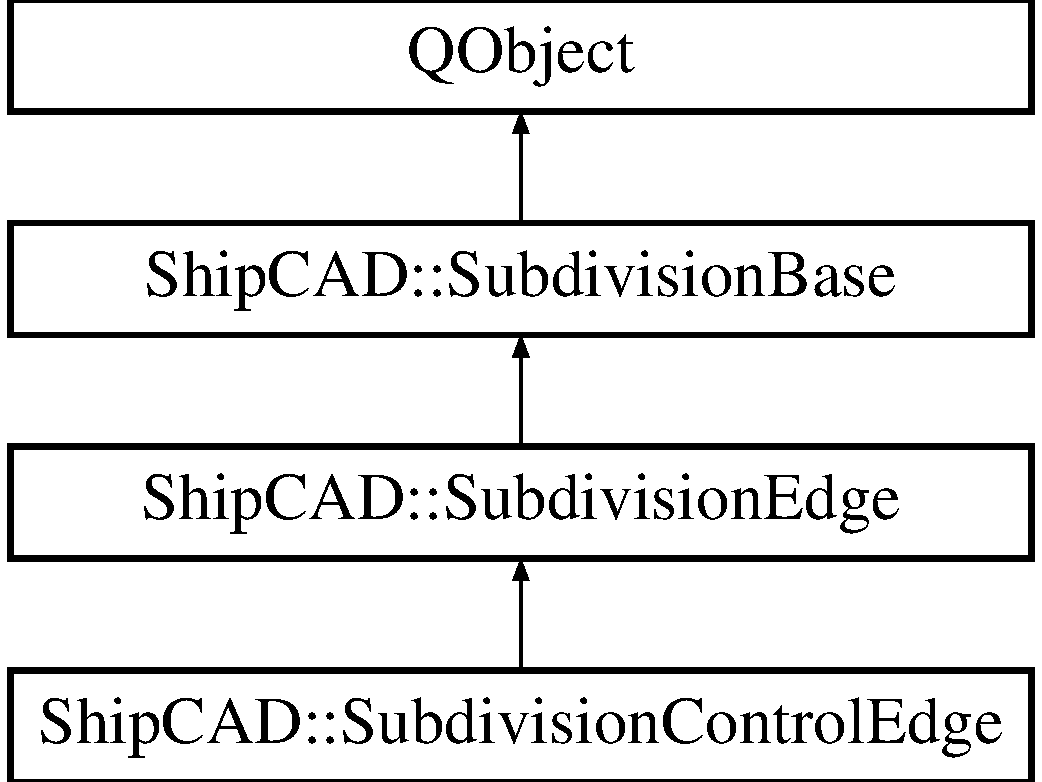
\includegraphics[height=4.000000cm]{classShipCAD_1_1SubdivisionControlEdge}
\end{center}
\end{figure}
\subsection*{Public Member Functions}
\begin{DoxyCompactItemize}
\item 
\hyperlink{classShipCAD_1_1SubdivisionControlEdge_aca48edfc1bb45a645708aecc8c8c3e04}{Subdivision\-Control\-Edge} (\hyperlink{classShipCAD_1_1SubdivisionSurface}{Subdivision\-Surface} $\ast$owner)
\item 
virtual \hyperlink{classShipCAD_1_1SubdivisionControlEdge_ad5e8153693c900a598618277cdeccd15}{$\sim$\-Subdivision\-Control\-Edge} ()
\item 
\hyperlink{classShipCAD_1_1SubdivisionControlPoint}{Subdivision\-Control\-Point} $\ast$ \hyperlink{classShipCAD_1_1SubdivisionControlEdge_a4839a04d67e4240b570fd23be711bc10}{insert\-Control\-Point} (const Q\-Vector3\-D \&p)
\item 
void \hyperlink{classShipCAD_1_1SubdivisionControlEdge_a07c67ddff486dc5e4ad830f549b32099}{trace} ()
\item 
size\-\_\-t \hyperlink{classShipCAD_1_1SubdivisionControlEdge_a0fb224ed7895deb9eb4cdb57ab9c451c}{get\-Index} ()
\item 
Q\-Color \hyperlink{classShipCAD_1_1SubdivisionControlEdge_a5cafa9a1fd8c93f10e2ae767608dfb26}{get\-Color} ()
\item 
virtual bool \hyperlink{classShipCAD_1_1SubdivisionControlEdge_a23adc8ad28860987b7b4866eada3c463}{is\-Boundary\-Edge} ()
\item 
bool \hyperlink{classShipCAD_1_1SubdivisionControlEdge_abcb240992ffb5637363341dbfd7003c7}{is\-Selected} ()
\item 
void \hyperlink{classShipCAD_1_1SubdivisionControlEdge_ae247e08eec97952d1835df03c8269829}{set\-Selected} (bool val)
\item 
bool \hyperlink{classShipCAD_1_1SubdivisionControlEdge_aaf83103b6772bf2387641b09194b12a6}{is\-Visible} ()
\item 
virtual void \hyperlink{classShipCAD_1_1SubdivisionControlEdge_a6b86017a5ea7fe487f6017071406e8c4}{draw} (\hyperlink{classShipCAD_1_1Viewport}{Viewport} \&vp, \hyperlink{classShipCAD_1_1LineShader}{Line\-Shader} $\ast$lineshader)
\item 
void \hyperlink{classShipCAD_1_1SubdivisionControlEdge_a0f48c4ce176a5de42e0a7c741aa129f5}{load\-Binary} (\hyperlink{classShipCAD_1_1FileBuffer}{File\-Buffer} \&source)
\item 
void \hyperlink{classShipCAD_1_1SubdivisionControlEdge_a572f4331ef0ab6f241583fc8d36cb93e}{save\-Binary} (\hyperlink{classShipCAD_1_1FileBuffer}{File\-Buffer} \&destination)
\item 
void \hyperlink{classShipCAD_1_1SubdivisionControlEdge_a318bf4102460ba91fd9e79fbde265ee3}{load\-From\-Stream} (size\-\_\-t \&lineno, Q\-String\-List \&strings)
\item 
void \hyperlink{classShipCAD_1_1SubdivisionControlEdge_a9228cf5bb5b09daf26eb4022f09337f0}{save\-To\-Stream} (Q\-String\-List \&strings)
\item 
virtual void \hyperlink{classShipCAD_1_1SubdivisionControlEdge_abdfa96ff05eff404214a92d38d7eb715}{dump} (std\-::ostream \&os, const char $\ast$prefix=\char`\"{}\char`\"{}) const 
\begin{DoxyCompactList}\small\item\em print out the element to a stream \end{DoxyCompactList}\end{DoxyCompactItemize}
\subsection*{Static Public Member Functions}
\begin{DoxyCompactItemize}
\item 
static \hyperlink{classShipCAD_1_1SubdivisionControlEdge}{Subdivision\-Control\-Edge} $\ast$ \hyperlink{classShipCAD_1_1SubdivisionControlEdge_a20fc507b201766b6e3d0560595946fac}{construct} (\hyperlink{classShipCAD_1_1SubdivisionSurface}{Subdivision\-Surface} $\ast$owner)
\end{DoxyCompactItemize}
\subsection*{Protected Member Functions}
\begin{DoxyCompactItemize}
\item 
void \hyperlink{classShipCAD_1_1SubdivisionControlEdge_acc4cee57db50beb1dcc6361f7f2c62af}{priv\-\_\-dump} (std\-::ostream \&os, const char $\ast$prefix) const 
\item 
void \hyperlink{classShipCAD_1_1SubdivisionControlEdge_aec6ff8caa6996ae5a9d2e58d5d2b0344}{priv\-\_\-trace} (\hyperlink{classShipCAD_1_1SubdivisionControlPoint}{Subdivision\-Control\-Point} $\ast$p)
\end{DoxyCompactItemize}
\subsection*{Protected Attributes}
\begin{DoxyCompactItemize}
\item 
bool \hyperlink{classShipCAD_1_1SubdivisionControlEdge_a8e67d30ef7ef87ff599f73b59c806f58}{\-\_\-selected}
\item 
bool \hyperlink{classShipCAD_1_1SubdivisionControlEdge_a8d49343e2b6ff0ab13653849af242740}{\-\_\-visible}
\end{DoxyCompactItemize}
\subsection*{Properties}
\begin{DoxyCompactItemize}
\item 
Q\-Color \hyperlink{classShipCAD_1_1SubdivisionControlEdge_a1aaeec9c0e1dc9d7b49dfe2913e8a0a7}{Color}
\item 
bool \hyperlink{classShipCAD_1_1SubdivisionControlEdge_a8d2d3e419649962262d049bde688caac}{Visible}
\item 
bool \hyperlink{classShipCAD_1_1SubdivisionControlEdge_a25279492599975df97efcaa124e09855}{Selected}
\end{DoxyCompactItemize}


\subsection{Detailed Description}


Definition at line 119 of file subdivedge.\-h.



\subsection{Constructor \& Destructor Documentation}
\hypertarget{classShipCAD_1_1SubdivisionControlEdge_aca48edfc1bb45a645708aecc8c8c3e04}{\index{Ship\-C\-A\-D\-::\-Subdivision\-Control\-Edge@{Ship\-C\-A\-D\-::\-Subdivision\-Control\-Edge}!Subdivision\-Control\-Edge@{Subdivision\-Control\-Edge}}
\index{Subdivision\-Control\-Edge@{Subdivision\-Control\-Edge}!ShipCAD::SubdivisionControlEdge@{Ship\-C\-A\-D\-::\-Subdivision\-Control\-Edge}}
\subsubsection[{Subdivision\-Control\-Edge}]{\setlength{\rightskip}{0pt plus 5cm}Subdivision\-Control\-Edge\-::\-Subdivision\-Control\-Edge (
\begin{DoxyParamCaption}
\item[{{\bf Subdivision\-Surface} $\ast$}]{owner}
\end{DoxyParamCaption}
)\hspace{0.3cm}{\ttfamily [explicit]}}}\label{classShipCAD_1_1SubdivisionControlEdge_aca48edfc1bb45a645708aecc8c8c3e04}


Definition at line 376 of file subdivedge.\-cpp.

\hypertarget{classShipCAD_1_1SubdivisionControlEdge_ad5e8153693c900a598618277cdeccd15}{\index{Ship\-C\-A\-D\-::\-Subdivision\-Control\-Edge@{Ship\-C\-A\-D\-::\-Subdivision\-Control\-Edge}!$\sim$\-Subdivision\-Control\-Edge@{$\sim$\-Subdivision\-Control\-Edge}}
\index{$\sim$\-Subdivision\-Control\-Edge@{$\sim$\-Subdivision\-Control\-Edge}!ShipCAD::SubdivisionControlEdge@{Ship\-C\-A\-D\-::\-Subdivision\-Control\-Edge}}
\subsubsection[{$\sim$\-Subdivision\-Control\-Edge}]{\setlength{\rightskip}{0pt plus 5cm}Subdivision\-Control\-Edge\-::$\sim$\-Subdivision\-Control\-Edge (
\begin{DoxyParamCaption}
{}
\end{DoxyParamCaption}
)\hspace{0.3cm}{\ttfamily [virtual]}}}\label{classShipCAD_1_1SubdivisionControlEdge_ad5e8153693c900a598618277cdeccd15}


Definition at line 382 of file subdivedge.\-cpp.



\subsection{Member Function Documentation}
\hypertarget{classShipCAD_1_1SubdivisionControlEdge_a20fc507b201766b6e3d0560595946fac}{\index{Ship\-C\-A\-D\-::\-Subdivision\-Control\-Edge@{Ship\-C\-A\-D\-::\-Subdivision\-Control\-Edge}!construct@{construct}}
\index{construct@{construct}!ShipCAD::SubdivisionControlEdge@{Ship\-C\-A\-D\-::\-Subdivision\-Control\-Edge}}
\subsubsection[{construct}]{\setlength{\rightskip}{0pt plus 5cm}{\bf Subdivision\-Control\-Edge} $\ast$ Subdivision\-Control\-Edge\-::construct (
\begin{DoxyParamCaption}
\item[{{\bf Subdivision\-Surface} $\ast$}]{owner}
\end{DoxyParamCaption}
)\hspace{0.3cm}{\ttfamily [static]}}}\label{classShipCAD_1_1SubdivisionControlEdge_a20fc507b201766b6e3d0560595946fac}


Definition at line 368 of file subdivedge.\-cpp.

\hypertarget{classShipCAD_1_1SubdivisionControlEdge_a6b86017a5ea7fe487f6017071406e8c4}{\index{Ship\-C\-A\-D\-::\-Subdivision\-Control\-Edge@{Ship\-C\-A\-D\-::\-Subdivision\-Control\-Edge}!draw@{draw}}
\index{draw@{draw}!ShipCAD::SubdivisionControlEdge@{Ship\-C\-A\-D\-::\-Subdivision\-Control\-Edge}}
\subsubsection[{draw}]{\setlength{\rightskip}{0pt plus 5cm}void Subdivision\-Control\-Edge\-::draw (
\begin{DoxyParamCaption}
\item[{{\bf Viewport} \&}]{vp, }
\item[{{\bf Line\-Shader} $\ast$}]{lineshader}
\end{DoxyParamCaption}
)\hspace{0.3cm}{\ttfamily [virtual]}}}\label{classShipCAD_1_1SubdivisionControlEdge_a6b86017a5ea7fe487f6017071406e8c4}


Definition at line 619 of file subdivedge.\-cpp.

\hypertarget{classShipCAD_1_1SubdivisionControlEdge_abdfa96ff05eff404214a92d38d7eb715}{\index{Ship\-C\-A\-D\-::\-Subdivision\-Control\-Edge@{Ship\-C\-A\-D\-::\-Subdivision\-Control\-Edge}!dump@{dump}}
\index{dump@{dump}!ShipCAD::SubdivisionControlEdge@{Ship\-C\-A\-D\-::\-Subdivision\-Control\-Edge}}
\subsubsection[{dump}]{\setlength{\rightskip}{0pt plus 5cm}void Subdivision\-Control\-Edge\-::dump (
\begin{DoxyParamCaption}
\item[{std\-::ostream \&}]{os, }
\item[{const char $\ast$}]{prefix = {\ttfamily \char`\"{}\char`\"{}}}
\end{DoxyParamCaption}
) const\hspace{0.3cm}{\ttfamily [virtual]}}}\label{classShipCAD_1_1SubdivisionControlEdge_abdfa96ff05eff404214a92d38d7eb715}


print out the element to a stream 


\begin{DoxyParams}{Parameters}
{\em os} & the output stream \\
\hline
{\em prefix} & string to prefix on each line output \\
\hline
\end{DoxyParams}


Reimplemented from \hyperlink{classShipCAD_1_1SubdivisionEdge_a14cc58877644ebd7b7ebffbdf8ef87f7}{Ship\-C\-A\-D\-::\-Subdivision\-Edge}.



Definition at line 686 of file subdivedge.\-cpp.

\hypertarget{classShipCAD_1_1SubdivisionControlEdge_a5cafa9a1fd8c93f10e2ae767608dfb26}{\index{Ship\-C\-A\-D\-::\-Subdivision\-Control\-Edge@{Ship\-C\-A\-D\-::\-Subdivision\-Control\-Edge}!get\-Color@{get\-Color}}
\index{get\-Color@{get\-Color}!ShipCAD::SubdivisionControlEdge@{Ship\-C\-A\-D\-::\-Subdivision\-Control\-Edge}}
\subsubsection[{get\-Color}]{\setlength{\rightskip}{0pt plus 5cm}Q\-Color Subdivision\-Control\-Edge\-::get\-Color (
\begin{DoxyParamCaption}
{}
\end{DoxyParamCaption}
)}}\label{classShipCAD_1_1SubdivisionControlEdge_a5cafa9a1fd8c93f10e2ae767608dfb26}


Definition at line 406 of file subdivedge.\-cpp.

\hypertarget{classShipCAD_1_1SubdivisionControlEdge_a0fb224ed7895deb9eb4cdb57ab9c451c}{\index{Ship\-C\-A\-D\-::\-Subdivision\-Control\-Edge@{Ship\-C\-A\-D\-::\-Subdivision\-Control\-Edge}!get\-Index@{get\-Index}}
\index{get\-Index@{get\-Index}!ShipCAD::SubdivisionControlEdge@{Ship\-C\-A\-D\-::\-Subdivision\-Control\-Edge}}
\subsubsection[{get\-Index}]{\setlength{\rightskip}{0pt plus 5cm}size\-\_\-t Subdivision\-Control\-Edge\-::get\-Index (
\begin{DoxyParamCaption}
{}
\end{DoxyParamCaption}
)}}\label{classShipCAD_1_1SubdivisionControlEdge_a0fb224ed7895deb9eb4cdb57ab9c451c}


Definition at line 420 of file subdivedge.\-cpp.

\hypertarget{classShipCAD_1_1SubdivisionControlEdge_a4839a04d67e4240b570fd23be711bc10}{\index{Ship\-C\-A\-D\-::\-Subdivision\-Control\-Edge@{Ship\-C\-A\-D\-::\-Subdivision\-Control\-Edge}!insert\-Control\-Point@{insert\-Control\-Point}}
\index{insert\-Control\-Point@{insert\-Control\-Point}!ShipCAD::SubdivisionControlEdge@{Ship\-C\-A\-D\-::\-Subdivision\-Control\-Edge}}
\subsubsection[{insert\-Control\-Point}]{\setlength{\rightskip}{0pt plus 5cm}{\bf Subdivision\-Control\-Point} $\ast$ Subdivision\-Control\-Edge\-::insert\-Control\-Point (
\begin{DoxyParamCaption}
\item[{const Q\-Vector3\-D \&}]{p}
\end{DoxyParamCaption}
)}}\label{classShipCAD_1_1SubdivisionControlEdge_a4839a04d67e4240b570fd23be711bc10}


Definition at line 481 of file subdivedge.\-cpp.

\hypertarget{classShipCAD_1_1SubdivisionControlEdge_a23adc8ad28860987b7b4866eada3c463}{\index{Ship\-C\-A\-D\-::\-Subdivision\-Control\-Edge@{Ship\-C\-A\-D\-::\-Subdivision\-Control\-Edge}!is\-Boundary\-Edge@{is\-Boundary\-Edge}}
\index{is\-Boundary\-Edge@{is\-Boundary\-Edge}!ShipCAD::SubdivisionControlEdge@{Ship\-C\-A\-D\-::\-Subdivision\-Control\-Edge}}
\subsubsection[{is\-Boundary\-Edge}]{\setlength{\rightskip}{0pt plus 5cm}bool Subdivision\-Control\-Edge\-::is\-Boundary\-Edge (
\begin{DoxyParamCaption}
{}
\end{DoxyParamCaption}
)\hspace{0.3cm}{\ttfamily [virtual]}}}\label{classShipCAD_1_1SubdivisionControlEdge_a23adc8ad28860987b7b4866eada3c463}


Reimplemented from \hyperlink{classShipCAD_1_1SubdivisionEdge_ad95a3ec8ba66deb74cbfd3d36428fc34}{Ship\-C\-A\-D\-::\-Subdivision\-Edge}.



Definition at line 425 of file subdivedge.\-cpp.

\hypertarget{classShipCAD_1_1SubdivisionControlEdge_abcb240992ffb5637363341dbfd7003c7}{\index{Ship\-C\-A\-D\-::\-Subdivision\-Control\-Edge@{Ship\-C\-A\-D\-::\-Subdivision\-Control\-Edge}!is\-Selected@{is\-Selected}}
\index{is\-Selected@{is\-Selected}!ShipCAD::SubdivisionControlEdge@{Ship\-C\-A\-D\-::\-Subdivision\-Control\-Edge}}
\subsubsection[{is\-Selected}]{\setlength{\rightskip}{0pt plus 5cm}bool Subdivision\-Control\-Edge\-::is\-Selected (
\begin{DoxyParamCaption}
{}
\end{DoxyParamCaption}
)}}\label{classShipCAD_1_1SubdivisionControlEdge_abcb240992ffb5637363341dbfd7003c7}


Definition at line 448 of file subdivedge.\-cpp.

\hypertarget{classShipCAD_1_1SubdivisionControlEdge_aaf83103b6772bf2387641b09194b12a6}{\index{Ship\-C\-A\-D\-::\-Subdivision\-Control\-Edge@{Ship\-C\-A\-D\-::\-Subdivision\-Control\-Edge}!is\-Visible@{is\-Visible}}
\index{is\-Visible@{is\-Visible}!ShipCAD::SubdivisionControlEdge@{Ship\-C\-A\-D\-::\-Subdivision\-Control\-Edge}}
\subsubsection[{is\-Visible}]{\setlength{\rightskip}{0pt plus 5cm}bool Subdivision\-Control\-Edge\-::is\-Visible (
\begin{DoxyParamCaption}
{}
\end{DoxyParamCaption}
)}}\label{classShipCAD_1_1SubdivisionControlEdge_aaf83103b6772bf2387641b09194b12a6}


Definition at line 453 of file subdivedge.\-cpp.

\hypertarget{classShipCAD_1_1SubdivisionControlEdge_a0f48c4ce176a5de42e0a7c741aa129f5}{\index{Ship\-C\-A\-D\-::\-Subdivision\-Control\-Edge@{Ship\-C\-A\-D\-::\-Subdivision\-Control\-Edge}!load\-Binary@{load\-Binary}}
\index{load\-Binary@{load\-Binary}!ShipCAD::SubdivisionControlEdge@{Ship\-C\-A\-D\-::\-Subdivision\-Control\-Edge}}
\subsubsection[{load\-Binary}]{\setlength{\rightskip}{0pt plus 5cm}void Subdivision\-Control\-Edge\-::load\-Binary (
\begin{DoxyParamCaption}
\item[{{\bf File\-Buffer} \&}]{source}
\end{DoxyParamCaption}
)}}\label{classShipCAD_1_1SubdivisionControlEdge_a0f48c4ce176a5de42e0a7c741aa129f5}


Definition at line 523 of file subdivedge.\-cpp.

\hypertarget{classShipCAD_1_1SubdivisionControlEdge_a318bf4102460ba91fd9e79fbde265ee3}{\index{Ship\-C\-A\-D\-::\-Subdivision\-Control\-Edge@{Ship\-C\-A\-D\-::\-Subdivision\-Control\-Edge}!load\-From\-Stream@{load\-From\-Stream}}
\index{load\-From\-Stream@{load\-From\-Stream}!ShipCAD::SubdivisionControlEdge@{Ship\-C\-A\-D\-::\-Subdivision\-Control\-Edge}}
\subsubsection[{load\-From\-Stream}]{\setlength{\rightskip}{0pt plus 5cm}void Subdivision\-Control\-Edge\-::load\-From\-Stream (
\begin{DoxyParamCaption}
\item[{size\-\_\-t \&}]{lineno, }
\item[{Q\-String\-List \&}]{strings}
\end{DoxyParamCaption}
)}}\label{classShipCAD_1_1SubdivisionControlEdge_a318bf4102460ba91fd9e79fbde265ee3}


Definition at line 540 of file subdivedge.\-cpp.

\hypertarget{classShipCAD_1_1SubdivisionControlEdge_acc4cee57db50beb1dcc6361f7f2c62af}{\index{Ship\-C\-A\-D\-::\-Subdivision\-Control\-Edge@{Ship\-C\-A\-D\-::\-Subdivision\-Control\-Edge}!priv\-\_\-dump@{priv\-\_\-dump}}
\index{priv\-\_\-dump@{priv\-\_\-dump}!ShipCAD::SubdivisionControlEdge@{Ship\-C\-A\-D\-::\-Subdivision\-Control\-Edge}}
\subsubsection[{priv\-\_\-dump}]{\setlength{\rightskip}{0pt plus 5cm}void Subdivision\-Control\-Edge\-::priv\-\_\-dump (
\begin{DoxyParamCaption}
\item[{std\-::ostream \&}]{os, }
\item[{const char $\ast$}]{prefix}
\end{DoxyParamCaption}
) const\hspace{0.3cm}{\ttfamily [protected]}}}\label{classShipCAD_1_1SubdivisionControlEdge_acc4cee57db50beb1dcc6361f7f2c62af}


Definition at line 694 of file subdivedge.\-cpp.

\hypertarget{classShipCAD_1_1SubdivisionControlEdge_aec6ff8caa6996ae5a9d2e58d5d2b0344}{\index{Ship\-C\-A\-D\-::\-Subdivision\-Control\-Edge@{Ship\-C\-A\-D\-::\-Subdivision\-Control\-Edge}!priv\-\_\-trace@{priv\-\_\-trace}}
\index{priv\-\_\-trace@{priv\-\_\-trace}!ShipCAD::SubdivisionControlEdge@{Ship\-C\-A\-D\-::\-Subdivision\-Control\-Edge}}
\subsubsection[{priv\-\_\-trace}]{\setlength{\rightskip}{0pt plus 5cm}void Subdivision\-Control\-Edge\-::priv\-\_\-trace (
\begin{DoxyParamCaption}
\item[{{\bf Subdivision\-Control\-Point} $\ast$}]{p}
\end{DoxyParamCaption}
)\hspace{0.3cm}{\ttfamily [protected]}}}\label{classShipCAD_1_1SubdivisionControlEdge_aec6ff8caa6996ae5a9d2e58d5d2b0344}


Definition at line 580 of file subdivedge.\-cpp.

\hypertarget{classShipCAD_1_1SubdivisionControlEdge_a572f4331ef0ab6f241583fc8d36cb93e}{\index{Ship\-C\-A\-D\-::\-Subdivision\-Control\-Edge@{Ship\-C\-A\-D\-::\-Subdivision\-Control\-Edge}!save\-Binary@{save\-Binary}}
\index{save\-Binary@{save\-Binary}!ShipCAD::SubdivisionControlEdge@{Ship\-C\-A\-D\-::\-Subdivision\-Control\-Edge}}
\subsubsection[{save\-Binary}]{\setlength{\rightskip}{0pt plus 5cm}void Subdivision\-Control\-Edge\-::save\-Binary (
\begin{DoxyParamCaption}
\item[{{\bf File\-Buffer} \&}]{destination}
\end{DoxyParamCaption}
)}}\label{classShipCAD_1_1SubdivisionControlEdge_a572f4331ef0ab6f241583fc8d36cb93e}


Definition at line 572 of file subdivedge.\-cpp.

\hypertarget{classShipCAD_1_1SubdivisionControlEdge_a9228cf5bb5b09daf26eb4022f09337f0}{\index{Ship\-C\-A\-D\-::\-Subdivision\-Control\-Edge@{Ship\-C\-A\-D\-::\-Subdivision\-Control\-Edge}!save\-To\-Stream@{save\-To\-Stream}}
\index{save\-To\-Stream@{save\-To\-Stream}!ShipCAD::SubdivisionControlEdge@{Ship\-C\-A\-D\-::\-Subdivision\-Control\-Edge}}
\subsubsection[{save\-To\-Stream}]{\setlength{\rightskip}{0pt plus 5cm}void Subdivision\-Control\-Edge\-::save\-To\-Stream (
\begin{DoxyParamCaption}
\item[{Q\-String\-List \&}]{strings}
\end{DoxyParamCaption}
)}}\label{classShipCAD_1_1SubdivisionControlEdge_a9228cf5bb5b09daf26eb4022f09337f0}


Definition at line 562 of file subdivedge.\-cpp.

\hypertarget{classShipCAD_1_1SubdivisionControlEdge_ae247e08eec97952d1835df03c8269829}{\index{Ship\-C\-A\-D\-::\-Subdivision\-Control\-Edge@{Ship\-C\-A\-D\-::\-Subdivision\-Control\-Edge}!set\-Selected@{set\-Selected}}
\index{set\-Selected@{set\-Selected}!ShipCAD::SubdivisionControlEdge@{Ship\-C\-A\-D\-::\-Subdivision\-Control\-Edge}}
\subsubsection[{set\-Selected}]{\setlength{\rightskip}{0pt plus 5cm}void Subdivision\-Control\-Edge\-::set\-Selected (
\begin{DoxyParamCaption}
\item[{bool}]{val}
\end{DoxyParamCaption}
)}}\label{classShipCAD_1_1SubdivisionControlEdge_ae247e08eec97952d1835df03c8269829}


Definition at line 440 of file subdivedge.\-cpp.

\hypertarget{classShipCAD_1_1SubdivisionControlEdge_a07c67ddff486dc5e4ad830f549b32099}{\index{Ship\-C\-A\-D\-::\-Subdivision\-Control\-Edge@{Ship\-C\-A\-D\-::\-Subdivision\-Control\-Edge}!trace@{trace}}
\index{trace@{trace}!ShipCAD::SubdivisionControlEdge@{Ship\-C\-A\-D\-::\-Subdivision\-Control\-Edge}}
\subsubsection[{trace}]{\setlength{\rightskip}{0pt plus 5cm}void Subdivision\-Control\-Edge\-::trace (
\begin{DoxyParamCaption}
{}
\end{DoxyParamCaption}
)}}\label{classShipCAD_1_1SubdivisionControlEdge_a07c67ddff486dc5e4ad830f549b32099}


Definition at line 609 of file subdivedge.\-cpp.



\subsection{Member Data Documentation}
\hypertarget{classShipCAD_1_1SubdivisionControlEdge_a8e67d30ef7ef87ff599f73b59c806f58}{\index{Ship\-C\-A\-D\-::\-Subdivision\-Control\-Edge@{Ship\-C\-A\-D\-::\-Subdivision\-Control\-Edge}!\-\_\-selected@{\-\_\-selected}}
\index{\-\_\-selected@{\-\_\-selected}!ShipCAD::SubdivisionControlEdge@{Ship\-C\-A\-D\-::\-Subdivision\-Control\-Edge}}
\subsubsection[{\-\_\-selected}]{\setlength{\rightskip}{0pt plus 5cm}bool Ship\-C\-A\-D\-::\-Subdivision\-Control\-Edge\-::\-\_\-selected\hspace{0.3cm}{\ttfamily [protected]}}}\label{classShipCAD_1_1SubdivisionControlEdge_a8e67d30ef7ef87ff599f73b59c806f58}


Definition at line 165 of file subdivedge.\-h.

\hypertarget{classShipCAD_1_1SubdivisionControlEdge_a8d49343e2b6ff0ab13653849af242740}{\index{Ship\-C\-A\-D\-::\-Subdivision\-Control\-Edge@{Ship\-C\-A\-D\-::\-Subdivision\-Control\-Edge}!\-\_\-visible@{\-\_\-visible}}
\index{\-\_\-visible@{\-\_\-visible}!ShipCAD::SubdivisionControlEdge@{Ship\-C\-A\-D\-::\-Subdivision\-Control\-Edge}}
\subsubsection[{\-\_\-visible}]{\setlength{\rightskip}{0pt plus 5cm}bool Ship\-C\-A\-D\-::\-Subdivision\-Control\-Edge\-::\-\_\-visible\hspace{0.3cm}{\ttfamily [protected]}}}\label{classShipCAD_1_1SubdivisionControlEdge_a8d49343e2b6ff0ab13653849af242740}


Definition at line 166 of file subdivedge.\-h.



\subsection{Property Documentation}
\hypertarget{classShipCAD_1_1SubdivisionControlEdge_a1aaeec9c0e1dc9d7b49dfe2913e8a0a7}{\index{Ship\-C\-A\-D\-::\-Subdivision\-Control\-Edge@{Ship\-C\-A\-D\-::\-Subdivision\-Control\-Edge}!Color@{Color}}
\index{Color@{Color}!ShipCAD::SubdivisionControlEdge@{Ship\-C\-A\-D\-::\-Subdivision\-Control\-Edge}}
\subsubsection[{Color}]{\setlength{\rightskip}{0pt plus 5cm}Q\-Color Ship\-C\-A\-D\-::\-Subdivision\-Control\-Edge\-::\-Color\hspace{0.3cm}{\ttfamily [read]}}}\label{classShipCAD_1_1SubdivisionControlEdge_a1aaeec9c0e1dc9d7b49dfe2913e8a0a7}


Definition at line 122 of file subdivedge.\-h.

\hypertarget{classShipCAD_1_1SubdivisionControlEdge_a25279492599975df97efcaa124e09855}{\index{Ship\-C\-A\-D\-::\-Subdivision\-Control\-Edge@{Ship\-C\-A\-D\-::\-Subdivision\-Control\-Edge}!Selected@{Selected}}
\index{Selected@{Selected}!ShipCAD::SubdivisionControlEdge@{Ship\-C\-A\-D\-::\-Subdivision\-Control\-Edge}}
\subsubsection[{Selected}]{\setlength{\rightskip}{0pt plus 5cm}bool Ship\-C\-A\-D\-::\-Subdivision\-Control\-Edge\-::\-Selected\hspace{0.3cm}{\ttfamily [read]}, {\ttfamily [write]}}}\label{classShipCAD_1_1SubdivisionControlEdge_a25279492599975df97efcaa124e09855}


Definition at line 124 of file subdivedge.\-h.

\hypertarget{classShipCAD_1_1SubdivisionControlEdge_a8d2d3e419649962262d049bde688caac}{\index{Ship\-C\-A\-D\-::\-Subdivision\-Control\-Edge@{Ship\-C\-A\-D\-::\-Subdivision\-Control\-Edge}!Visible@{Visible}}
\index{Visible@{Visible}!ShipCAD::SubdivisionControlEdge@{Ship\-C\-A\-D\-::\-Subdivision\-Control\-Edge}}
\subsubsection[{Visible}]{\setlength{\rightskip}{0pt plus 5cm}bool Ship\-C\-A\-D\-::\-Subdivision\-Control\-Edge\-::\-Visible\hspace{0.3cm}{\ttfamily [read]}}}\label{classShipCAD_1_1SubdivisionControlEdge_a8d2d3e419649962262d049bde688caac}


Definition at line 123 of file subdivedge.\-h.



The documentation for this class was generated from the following files\-:\begin{DoxyCompactItemize}
\item 
Ship\-C\-A\-Dlib/\hyperlink{subdivedge_8h}{subdivedge.\-h}\item 
Ship\-C\-A\-Dlib/\hyperlink{subdivedge_8cpp}{subdivedge.\-cpp}\end{DoxyCompactItemize}

\hypertarget{classShipCAD_1_1SubdivisionControlFace}{\section{Ship\-C\-A\-D\-:\-:Subdivision\-Control\-Face Class Reference}
\label{classShipCAD_1_1SubdivisionControlFace}\index{Ship\-C\-A\-D\-::\-Subdivision\-Control\-Face@{Ship\-C\-A\-D\-::\-Subdivision\-Control\-Face}}
}


{\ttfamily \#include $<$subdivface.\-h$>$}

Inheritance diagram for Ship\-C\-A\-D\-:\-:Subdivision\-Control\-Face\-:\begin{figure}[H]
\begin{center}
\leavevmode
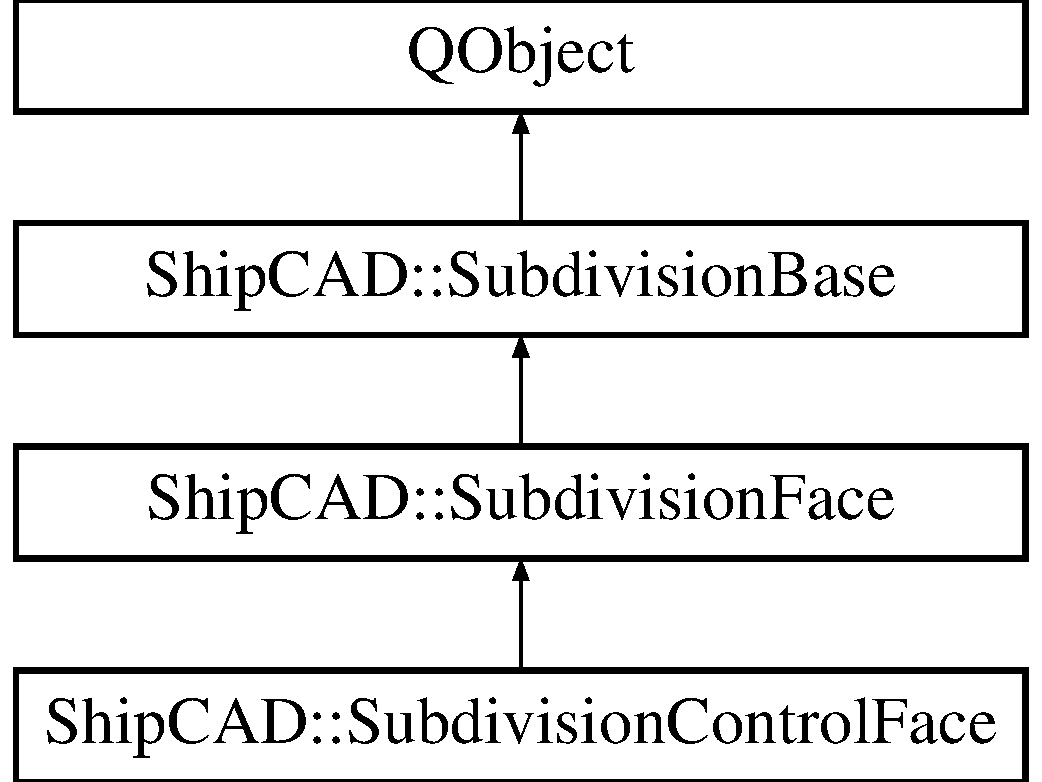
\includegraphics[height=3.000000cm]{classShipCAD_1_1SubdivisionControlFace}
\end{center}
\end{figure}
\subsection*{Public Member Functions}
\begin{DoxyCompactItemize}
\item 
\hyperlink{classShipCAD_1_1SubdivisionControlFace_a9316495869082b0e3e27092118913644}{Subdivision\-Control\-Face} (\hyperlink{classShipCAD_1_1SubdivisionSurface}{Subdivision\-Surface} $\ast$owner)
\begin{DoxyCompactList}\small\item\em Constructor. \end{DoxyCompactList}\item 
virtual \hyperlink{classShipCAD_1_1SubdivisionControlFace_a7b092e764ec2708674afdb210196f761}{$\sim$\-Subdivision\-Control\-Face} ()
\item 
void \hyperlink{classShipCAD_1_1SubdivisionControlFace_a611c74ce3f346a745d4a694f5aab4ec2}{calc\-Extents} ()
\begin{DoxyCompactList}\small\item\em get min/max coordinate amongst all children \end{DoxyCompactList}\item 
virtual void \hyperlink{classShipCAD_1_1SubdivisionControlFace_ad168e31f0ef2537b3cd0f58b0c1c54e2}{clear} ()
\begin{DoxyCompactList}\small\item\em reset attributes to default values \end{DoxyCompactList}\item 
void \hyperlink{classShipCAD_1_1SubdivisionControlFace_a1501212af025c7e33ede929d50a76651}{clear\-Children} ()
\begin{DoxyCompactList}\small\item\em remove all child faces and edges \end{DoxyCompactList}\item 
void \hyperlink{classShipCAD_1_1SubdivisionControlFace_a390a79e26ced82b4a879aebd0c1dc862}{clear\-Control\-Edges} ()
\begin{DoxyCompactList}\small\item\em remove all control edges of this face \end{DoxyCompactList}\item 
\hyperlink{classShipCAD_1_1SubdivisionControlEdge}{Subdivision\-Control\-Edge} $\ast$ \hyperlink{classShipCAD_1_1SubdivisionControlFace_af585a1c8300791375b2df87fe2ebc4f5}{insert\-Control\-Edge} (\hyperlink{classShipCAD_1_1SubdivisionControlPoint}{Subdivision\-Control\-Point} $\ast$p1, \hyperlink{classShipCAD_1_1SubdivisionControlPoint}{Subdivision\-Control\-Point} $\ast$p2)
\begin{DoxyCompactList}\small\item\em add a control edge \end{DoxyCompactList}\item 
void \hyperlink{classShipCAD_1_1SubdivisionControlFace_a1c5253075cbe1f05ba004bee4edb8698}{remove\-References} ()
\begin{DoxyCompactList}\small\item\em Removes this face and all edges from points. \end{DoxyCompactList}\item 
virtual void \hyperlink{classShipCAD_1_1SubdivisionControlFace_aa17b5bb33ad87a4fa1e618156c171c64}{subdivide} (std\-::vector$<$ std\-::pair$<$ \hyperlink{classShipCAD_1_1SubdivisionPoint}{Subdivision\-Point} $\ast$, \hyperlink{classShipCAD_1_1SubdivisionPoint}{Subdivision\-Point} $\ast$ $>$ $>$ \&vertexpoints, std\-::vector$<$ std\-::pair$<$ \hyperlink{classShipCAD_1_1SubdivisionEdge}{Subdivision\-Edge} $\ast$, \hyperlink{classShipCAD_1_1SubdivisionPoint}{Subdivision\-Point} $\ast$ $>$ $>$ \&edgepoints, std\-::vector$<$ std\-::pair$<$ \hyperlink{classShipCAD_1_1SubdivisionFace}{Subdivision\-Face} $\ast$, \hyperlink{classShipCAD_1_1SubdivisionPoint}{Subdivision\-Point} $\ast$ $>$ $>$ \&facepoints, std\-::vector$<$ \hyperlink{classShipCAD_1_1SubdivisionEdge}{Subdivision\-Edge} $\ast$ $>$ \&controledges)
\begin{DoxyCompactList}\small\item\em subdivide the face \end{DoxyCompactList}\item 
void \hyperlink{classShipCAD_1_1SubdivisionControlFace_a768d000d2891ca110d6eb804abf80351}{trace} ()
\begin{DoxyCompactList}\small\item\em select all control faces connected to this one \end{DoxyCompactList}\item 
\hyperlink{classShipCAD_1_1SubdivisionLayer}{Subdivision\-Layer} $\ast$ \hyperlink{classShipCAD_1_1SubdivisionControlFace_a0eff0f187a3c95f0541fb29eda112cd6}{get\-Layer} ()
\item 
void \hyperlink{classShipCAD_1_1SubdivisionControlFace_a23631dfffd1c3ad7fc59537a4684fa01}{set\-Layer} (\hyperlink{classShipCAD_1_1SubdivisionLayer}{Subdivision\-Layer} $\ast$layer)
\item 
\hyperlink{classShipCAD_1_1SubdivisionFace}{Subdivision\-Face} $\ast$ \hyperlink{classShipCAD_1_1SubdivisionControlFace_a2c25793e1bed9472121e9126bacac3ce}{get\-Child} (size\-\_\-t index)
\item 
size\-\_\-t \hyperlink{classShipCAD_1_1SubdivisionControlFace_aa4a26c00b8b77c0a9d78640fe465eeb1}{number\-Of\-Children} ()
\item 
Q\-Color \hyperlink{classShipCAD_1_1SubdivisionControlFace_a8a350fe4fec2ee93228ed9400a6f145c}{get\-Color} ()
\item 
\hyperlink{classShipCAD_1_1SubdivisionEdge}{Subdivision\-Edge} $\ast$ \hyperlink{classShipCAD_1_1SubdivisionControlFace_accfc3e8e3d79a2303126e44e6fdb1728}{get\-Control\-Edge} (size\-\_\-t index)
\item 
size\-\_\-t \hyperlink{classShipCAD_1_1SubdivisionControlFace_a11fd0577b7d09f1724be612af0c903a8}{number\-Of\-Control\-Edges} ()
\item 
\hyperlink{classShipCAD_1_1SubdivisionEdge}{Subdivision\-Edge} $\ast$ \hyperlink{classShipCAD_1_1SubdivisionControlFace_a37af31abc48d84d607c15158ad7c6a2a}{get\-Edge} (size\-\_\-t index)
\item 
size\-\_\-t \hyperlink{classShipCAD_1_1SubdivisionControlFace_a03ddd0f14ecc3631d1a7a2653ab0df7f}{number\-Of\-Edges} ()
\item 
size\-\_\-t \hyperlink{classShipCAD_1_1SubdivisionControlFace_a72f906db976c6530f0f2d4c03701ad15}{get\-Index} ()
\item 
bool \hyperlink{classShipCAD_1_1SubdivisionControlFace_ab56a2d4c3fccb7a578def71d286ee03c}{is\-Selected} ()
\item 
bool \hyperlink{classShipCAD_1_1SubdivisionControlFace_a2a722717e127bac12e3b81f4664fc568}{is\-Visible} ()
\item 
void \hyperlink{classShipCAD_1_1SubdivisionControlFace_a2ce580378cd200faec6a24d9d794c68e}{set\-Selected} (bool val)
\item 
Q\-Vector3\-D \hyperlink{classShipCAD_1_1SubdivisionControlFace_af78d2fd0849815610be193c99f04f5d7}{get\-Min} ()
\item 
Q\-Vector3\-D \hyperlink{classShipCAD_1_1SubdivisionControlFace_a4855077b5641cc8e644250d30cdd2629}{get\-Max} ()
\item 
std\-::vector$<$ \hyperlink{classShipCAD_1_1SubdivisionFace}{Subdivision\-Face} $\ast$ $>$\\*
\-::iterator \hyperlink{classShipCAD_1_1SubdivisionControlFace_ad20ed50df8ddd91c4aa04eb482ab0fa0}{children\-Begin} ()
\item 
std\-::vector$<$ \hyperlink{classShipCAD_1_1SubdivisionFace}{Subdivision\-Face} $\ast$ $>$\\*
\-::iterator \hyperlink{classShipCAD_1_1SubdivisionControlFace_acff2f413eceb70e345640c4519fb50bb}{children\-End} ()
\item 
void \hyperlink{classShipCAD_1_1SubdivisionControlFace_aa5ba43707787cde6e99cd645708e9200}{load\-Binary} (\hyperlink{classShipCAD_1_1FileBuffer}{File\-Buffer} \&source)
\item 
void \hyperlink{classShipCAD_1_1SubdivisionControlFace_a562b877e868dbd86ffe2c864232e1b78}{save\-Binary} (\hyperlink{classShipCAD_1_1FileBuffer}{File\-Buffer} \&destination)
\item 
void \hyperlink{classShipCAD_1_1SubdivisionControlFace_aecc7636c397ca5669cf7ddb995feac03}{save\-To\-D\-X\-F} (Q\-String\-List \&strings)
\item 
void \hyperlink{classShipCAD_1_1SubdivisionControlFace_a8a618958b27b97dd6da2473e130d7a8e}{save\-To\-Stream} (Q\-String\-List \&strings)
\item 
void \hyperlink{classShipCAD_1_1SubdivisionControlFace_ae06e29e54f93c529875bbd66b32ad3e7}{load\-From\-Stream} (size\-\_\-t \&lineno, Q\-String\-List \&strings)
\item 
virtual void \hyperlink{classShipCAD_1_1SubdivisionControlFace_ac253493bccd91108d936b651e72b46f8}{draw} (\hyperlink{classShipCAD_1_1Viewport}{Viewport} \&vp, \hyperlink{classShipCAD_1_1LineShader}{Line\-Shader} $\ast$lineshader)
\item 
virtual void \hyperlink{classShipCAD_1_1SubdivisionControlFace_a38631a5e4c99d1d183d61a0fe3fb47ed}{draw\-Faces} (\hyperlink{classShipCAD_1_1Viewport}{Viewport} \&vp, \hyperlink{classShipCAD_1_1FaceShader}{Face\-Shader} $\ast$monoshader)
\item 
virtual void \hyperlink{classShipCAD_1_1SubdivisionControlFace_aaf9226150996743d8d2ea560083ad1d8}{draw\-Curvature\-Faces} (\hyperlink{classShipCAD_1_1Viewport}{Viewport} \&vp, float Min\-Curvature, float Max\-Curvature)
\item 
virtual void \hyperlink{classShipCAD_1_1SubdivisionControlFace_a947868fba3e9bb6c587847fb9245c9ff}{dump} (std\-::ostream \&os, const char $\ast$prefix=\char`\"{}\char`\"{}) const 
\begin{DoxyCompactList}\small\item\em print out the element to a stream \end{DoxyCompactList}\end{DoxyCompactItemize}
\subsection*{Static Public Member Functions}
\begin{DoxyCompactItemize}
\item 
static \hyperlink{classShipCAD_1_1SubdivisionControlFace}{Subdivision\-Control\-Face} $\ast$ \hyperlink{classShipCAD_1_1SubdivisionControlFace_a4117f55ab3ec27bebd933f2992bc5dcd}{construct} (\hyperlink{classShipCAD_1_1SubdivisionSurface}{Subdivision\-Surface} $\ast$owner)
\end{DoxyCompactItemize}
\subsection*{Protected Member Functions}
\begin{DoxyCompactItemize}
\item 
void \hyperlink{classShipCAD_1_1SubdivisionControlFace_a224ce57a8d9d631eef63cccd8e0113f9}{priv\-\_\-dump} (std\-::ostream \&os, const char $\ast$prefix) const 
\item 
void \hyperlink{classShipCAD_1_1SubdivisionControlFace_aa6035e53cd1e32a9bd9e9f9800c9f7d4}{find\-Attached\-Faces} (std\-::vector$<$ \hyperlink{classShipCAD_1_1SubdivisionControlFace}{Subdivision\-Control\-Face} $\ast$ $>$ \&todo\-\_\-list, \hyperlink{classShipCAD_1_1SubdivisionControlFace}{Subdivision\-Control\-Face} $\ast$face)
\end{DoxyCompactItemize}
\subsection*{Protected Attributes}
\begin{DoxyCompactItemize}
\item 
\hyperlink{classShipCAD_1_1SubdivisionLayer}{Subdivision\-Layer} $\ast$ \hyperlink{classShipCAD_1_1SubdivisionControlFace_aee1990d4db7127ba59117a65c1a6ce7e}{\-\_\-layer}
\item 
Q\-Vector3\-D \hyperlink{classShipCAD_1_1SubdivisionControlFace_aac4f577da0f5203059901c5e09814e1d}{\-\_\-min}
\item 
Q\-Vector3\-D \hyperlink{classShipCAD_1_1SubdivisionControlFace_a22411574593283209772872bc740535b}{\-\_\-max}
\item 
std\-::vector$<$ \hyperlink{classShipCAD_1_1SubdivisionFace}{Subdivision\-Face} $\ast$ $>$ \hyperlink{classShipCAD_1_1SubdivisionControlFace_a116749a1de58ad46f68ad7e92031e673}{\-\_\-children}
\item 
std\-::vector$<$ \hyperlink{classShipCAD_1_1SubdivisionEdge}{Subdivision\-Edge} $\ast$ $>$ \hyperlink{classShipCAD_1_1SubdivisionControlFace_a390f626d9999ab3ce48878b223ea1693}{\-\_\-edges}
\item 
std\-::vector$<$ \hyperlink{classShipCAD_1_1SubdivisionEdge}{Subdivision\-Edge} $\ast$ $>$ \hyperlink{classShipCAD_1_1SubdivisionControlFace_a33d7e2ecd5f42edf5492efb83df3856b}{\-\_\-control\-\_\-edges}
\end{DoxyCompactItemize}


\subsection{Detailed Description}


Definition at line 203 of file subdivface.\-h.



\subsection{Constructor \& Destructor Documentation}
\hypertarget{classShipCAD_1_1SubdivisionControlFace_a9316495869082b0e3e27092118913644}{\index{Ship\-C\-A\-D\-::\-Subdivision\-Control\-Face@{Ship\-C\-A\-D\-::\-Subdivision\-Control\-Face}!Subdivision\-Control\-Face@{Subdivision\-Control\-Face}}
\index{Subdivision\-Control\-Face@{Subdivision\-Control\-Face}!ShipCAD::SubdivisionControlFace@{Ship\-C\-A\-D\-::\-Subdivision\-Control\-Face}}
\subsubsection[{Subdivision\-Control\-Face}]{\setlength{\rightskip}{0pt plus 5cm}Subdivision\-Control\-Face\-::\-Subdivision\-Control\-Face (
\begin{DoxyParamCaption}
\item[{{\bf Subdivision\-Surface} $\ast$}]{owner}
\end{DoxyParamCaption}
)\hspace{0.3cm}{\ttfamily [explicit]}}}\label{classShipCAD_1_1SubdivisionControlFace_a9316495869082b0e3e27092118913644}


Constructor. 


\begin{DoxyParams}{Parameters}
{\em owner} & parent surface \\
\hline
\end{DoxyParams}


Definition at line 408 of file subdivface.\-cpp.

\hypertarget{classShipCAD_1_1SubdivisionControlFace_a7b092e764ec2708674afdb210196f761}{\index{Ship\-C\-A\-D\-::\-Subdivision\-Control\-Face@{Ship\-C\-A\-D\-::\-Subdivision\-Control\-Face}!$\sim$\-Subdivision\-Control\-Face@{$\sim$\-Subdivision\-Control\-Face}}
\index{$\sim$\-Subdivision\-Control\-Face@{$\sim$\-Subdivision\-Control\-Face}!ShipCAD::SubdivisionControlFace@{Ship\-C\-A\-D\-::\-Subdivision\-Control\-Face}}
\subsubsection[{$\sim$\-Subdivision\-Control\-Face}]{\setlength{\rightskip}{0pt plus 5cm}Subdivision\-Control\-Face\-::$\sim$\-Subdivision\-Control\-Face (
\begin{DoxyParamCaption}
{}
\end{DoxyParamCaption}
)\hspace{0.3cm}{\ttfamily [virtual]}}}\label{classShipCAD_1_1SubdivisionControlFace_a7b092e764ec2708674afdb210196f761}


Definition at line 414 of file subdivface.\-cpp.



\subsection{Member Function Documentation}
\hypertarget{classShipCAD_1_1SubdivisionControlFace_a611c74ce3f346a745d4a694f5aab4ec2}{\index{Ship\-C\-A\-D\-::\-Subdivision\-Control\-Face@{Ship\-C\-A\-D\-::\-Subdivision\-Control\-Face}!calc\-Extents@{calc\-Extents}}
\index{calc\-Extents@{calc\-Extents}!ShipCAD::SubdivisionControlFace@{Ship\-C\-A\-D\-::\-Subdivision\-Control\-Face}}
\subsubsection[{calc\-Extents}]{\setlength{\rightskip}{0pt plus 5cm}void Subdivision\-Control\-Face\-::calc\-Extents (
\begin{DoxyParamCaption}
{}
\end{DoxyParamCaption}
)}}\label{classShipCAD_1_1SubdivisionControlFace_a611c74ce3f346a745d4a694f5aab4ec2}


get min/max coordinate amongst all children 

For each child face, update the min and max value for this face. 

Definition at line 695 of file subdivface.\-cpp.

\hypertarget{classShipCAD_1_1SubdivisionControlFace_ad20ed50df8ddd91c4aa04eb482ab0fa0}{\index{Ship\-C\-A\-D\-::\-Subdivision\-Control\-Face@{Ship\-C\-A\-D\-::\-Subdivision\-Control\-Face}!children\-Begin@{children\-Begin}}
\index{children\-Begin@{children\-Begin}!ShipCAD::SubdivisionControlFace@{Ship\-C\-A\-D\-::\-Subdivision\-Control\-Face}}
\subsubsection[{children\-Begin}]{\setlength{\rightskip}{0pt plus 5cm}std\-::vector$<${\bf Subdivision\-Face}$\ast$$>$\-::iterator Ship\-C\-A\-D\-::\-Subdivision\-Control\-Face\-::children\-Begin (
\begin{DoxyParamCaption}
{}
\end{DoxyParamCaption}
)\hspace{0.3cm}{\ttfamily [inline]}}}\label{classShipCAD_1_1SubdivisionControlFace_ad20ed50df8ddd91c4aa04eb482ab0fa0}


Definition at line 302 of file subdivface.\-h.

\hypertarget{classShipCAD_1_1SubdivisionControlFace_acff2f413eceb70e345640c4519fb50bb}{\index{Ship\-C\-A\-D\-::\-Subdivision\-Control\-Face@{Ship\-C\-A\-D\-::\-Subdivision\-Control\-Face}!children\-End@{children\-End}}
\index{children\-End@{children\-End}!ShipCAD::SubdivisionControlFace@{Ship\-C\-A\-D\-::\-Subdivision\-Control\-Face}}
\subsubsection[{children\-End}]{\setlength{\rightskip}{0pt plus 5cm}std\-::vector$<${\bf Subdivision\-Face}$\ast$$>$\-::iterator Ship\-C\-A\-D\-::\-Subdivision\-Control\-Face\-::children\-End (
\begin{DoxyParamCaption}
{}
\end{DoxyParamCaption}
)\hspace{0.3cm}{\ttfamily [inline]}}}\label{classShipCAD_1_1SubdivisionControlFace_acff2f413eceb70e345640c4519fb50bb}


Definition at line 303 of file subdivface.\-h.

\hypertarget{classShipCAD_1_1SubdivisionControlFace_ad168e31f0ef2537b3cd0f58b0c1c54e2}{\index{Ship\-C\-A\-D\-::\-Subdivision\-Control\-Face@{Ship\-C\-A\-D\-::\-Subdivision\-Control\-Face}!clear@{clear}}
\index{clear@{clear}!ShipCAD::SubdivisionControlFace@{Ship\-C\-A\-D\-::\-Subdivision\-Control\-Face}}
\subsubsection[{clear}]{\setlength{\rightskip}{0pt plus 5cm}void Subdivision\-Control\-Face\-::clear (
\begin{DoxyParamCaption}
{}
\end{DoxyParamCaption}
)\hspace{0.3cm}{\ttfamily [virtual]}}}\label{classShipCAD_1_1SubdivisionControlFace_ad168e31f0ef2537b3cd0f58b0c1c54e2}


reset attributes to default values 



Reimplemented from \hyperlink{classShipCAD_1_1SubdivisionFace_a413ae7e76f559780c8a69e998974fb75}{Ship\-C\-A\-D\-::\-Subdivision\-Face}.



Definition at line 722 of file subdivface.\-cpp.

\hypertarget{classShipCAD_1_1SubdivisionControlFace_a1501212af025c7e33ede929d50a76651}{\index{Ship\-C\-A\-D\-::\-Subdivision\-Control\-Face@{Ship\-C\-A\-D\-::\-Subdivision\-Control\-Face}!clear\-Children@{clear\-Children}}
\index{clear\-Children@{clear\-Children}!ShipCAD::SubdivisionControlFace@{Ship\-C\-A\-D\-::\-Subdivision\-Control\-Face}}
\subsubsection[{clear\-Children}]{\setlength{\rightskip}{0pt plus 5cm}void Subdivision\-Control\-Face\-::clear\-Children (
\begin{DoxyParamCaption}
{}
\end{DoxyParamCaption}
)}}\label{classShipCAD_1_1SubdivisionControlFace_a1501212af025c7e33ede929d50a76651}


remove all child faces and edges 

Remove all child faces and edges and also remove them from the parent surface face and edge pools 

Definition at line 731 of file subdivface.\-cpp.

\hypertarget{classShipCAD_1_1SubdivisionControlFace_a390a79e26ced82b4a879aebd0c1dc862}{\index{Ship\-C\-A\-D\-::\-Subdivision\-Control\-Face@{Ship\-C\-A\-D\-::\-Subdivision\-Control\-Face}!clear\-Control\-Edges@{clear\-Control\-Edges}}
\index{clear\-Control\-Edges@{clear\-Control\-Edges}!ShipCAD::SubdivisionControlFace@{Ship\-C\-A\-D\-::\-Subdivision\-Control\-Face}}
\subsubsection[{clear\-Control\-Edges}]{\setlength{\rightskip}{0pt plus 5cm}void Ship\-C\-A\-D\-::\-Subdivision\-Control\-Face\-::clear\-Control\-Edges (
\begin{DoxyParamCaption}
{}
\end{DoxyParamCaption}
)\hspace{0.3cm}{\ttfamily [inline]}}}\label{classShipCAD_1_1SubdivisionControlFace_a390a79e26ced82b4a879aebd0c1dc862}


remove all control edges of this face 



Definition at line 232 of file subdivface.\-h.

\hypertarget{classShipCAD_1_1SubdivisionControlFace_a4117f55ab3ec27bebd933f2992bc5dcd}{\index{Ship\-C\-A\-D\-::\-Subdivision\-Control\-Face@{Ship\-C\-A\-D\-::\-Subdivision\-Control\-Face}!construct@{construct}}
\index{construct@{construct}!ShipCAD::SubdivisionControlFace@{Ship\-C\-A\-D\-::\-Subdivision\-Control\-Face}}
\subsubsection[{construct}]{\setlength{\rightskip}{0pt plus 5cm}{\bf Subdivision\-Control\-Face} $\ast$ Subdivision\-Control\-Face\-::construct (
\begin{DoxyParamCaption}
\item[{{\bf Subdivision\-Surface} $\ast$}]{owner}
\end{DoxyParamCaption}
)\hspace{0.3cm}{\ttfamily [static]}}}\label{classShipCAD_1_1SubdivisionControlFace_a4117f55ab3ec27bebd933f2992bc5dcd}


Definition at line 400 of file subdivface.\-cpp.

\hypertarget{classShipCAD_1_1SubdivisionControlFace_ac253493bccd91108d936b651e72b46f8}{\index{Ship\-C\-A\-D\-::\-Subdivision\-Control\-Face@{Ship\-C\-A\-D\-::\-Subdivision\-Control\-Face}!draw@{draw}}
\index{draw@{draw}!ShipCAD::SubdivisionControlFace@{Ship\-C\-A\-D\-::\-Subdivision\-Control\-Face}}
\subsubsection[{draw}]{\setlength{\rightskip}{0pt plus 5cm}void Subdivision\-Control\-Face\-::draw (
\begin{DoxyParamCaption}
\item[{{\bf Viewport} \&}]{vp, }
\item[{{\bf Line\-Shader} $\ast$}]{lineshader}
\end{DoxyParamCaption}
)\hspace{0.3cm}{\ttfamily [virtual]}}}\label{classShipCAD_1_1SubdivisionControlFace_ac253493bccd91108d936b651e72b46f8}


Definition at line 561 of file subdivface.\-cpp.

\hypertarget{classShipCAD_1_1SubdivisionControlFace_aaf9226150996743d8d2ea560083ad1d8}{\index{Ship\-C\-A\-D\-::\-Subdivision\-Control\-Face@{Ship\-C\-A\-D\-::\-Subdivision\-Control\-Face}!draw\-Curvature\-Faces@{draw\-Curvature\-Faces}}
\index{draw\-Curvature\-Faces@{draw\-Curvature\-Faces}!ShipCAD::SubdivisionControlFace@{Ship\-C\-A\-D\-::\-Subdivision\-Control\-Face}}
\subsubsection[{draw\-Curvature\-Faces}]{\setlength{\rightskip}{0pt plus 5cm}void Subdivision\-Control\-Face\-::draw\-Curvature\-Faces (
\begin{DoxyParamCaption}
\item[{{\bf Viewport} \&}]{vp, }
\item[{float}]{Min\-Curvature, }
\item[{float}]{Max\-Curvature}
\end{DoxyParamCaption}
)\hspace{0.3cm}{\ttfamily [virtual]}}}\label{classShipCAD_1_1SubdivisionControlFace_aaf9226150996743d8d2ea560083ad1d8}


Definition at line 556 of file subdivface.\-cpp.

\hypertarget{classShipCAD_1_1SubdivisionControlFace_a38631a5e4c99d1d183d61a0fe3fb47ed}{\index{Ship\-C\-A\-D\-::\-Subdivision\-Control\-Face@{Ship\-C\-A\-D\-::\-Subdivision\-Control\-Face}!draw\-Faces@{draw\-Faces}}
\index{draw\-Faces@{draw\-Faces}!ShipCAD::SubdivisionControlFace@{Ship\-C\-A\-D\-::\-Subdivision\-Control\-Face}}
\subsubsection[{draw\-Faces}]{\setlength{\rightskip}{0pt plus 5cm}void Subdivision\-Control\-Face\-::draw\-Faces (
\begin{DoxyParamCaption}
\item[{{\bf Viewport} \&}]{vp, }
\item[{{\bf Face\-Shader} $\ast$}]{monoshader}
\end{DoxyParamCaption}
)\hspace{0.3cm}{\ttfamily [virtual]}}}\label{classShipCAD_1_1SubdivisionControlFace_a38631a5e4c99d1d183d61a0fe3fb47ed}


Definition at line 440 of file subdivface.\-cpp.

\hypertarget{classShipCAD_1_1SubdivisionControlFace_a947868fba3e9bb6c587847fb9245c9ff}{\index{Ship\-C\-A\-D\-::\-Subdivision\-Control\-Face@{Ship\-C\-A\-D\-::\-Subdivision\-Control\-Face}!dump@{dump}}
\index{dump@{dump}!ShipCAD::SubdivisionControlFace@{Ship\-C\-A\-D\-::\-Subdivision\-Control\-Face}}
\subsubsection[{dump}]{\setlength{\rightskip}{0pt plus 5cm}void Subdivision\-Control\-Face\-::dump (
\begin{DoxyParamCaption}
\item[{std\-::ostream \&}]{os, }
\item[{const char $\ast$}]{prefix = {\ttfamily \char`\"{}\char`\"{}}}
\end{DoxyParamCaption}
) const\hspace{0.3cm}{\ttfamily [virtual]}}}\label{classShipCAD_1_1SubdivisionControlFace_a947868fba3e9bb6c587847fb9245c9ff}


print out the element to a stream 


\begin{DoxyParams}{Parameters}
{\em os} & the output stream \\
\hline
{\em prefix} & string to prefix on each line output \\
\hline
\end{DoxyParams}


Reimplemented from \hyperlink{classShipCAD_1_1SubdivisionFace_aa5bd261ae5fc0a1c7fe8cc5328b8477f}{Ship\-C\-A\-D\-::\-Subdivision\-Face}.



Definition at line 965 of file subdivface.\-cpp.

\hypertarget{classShipCAD_1_1SubdivisionControlFace_aa6035e53cd1e32a9bd9e9f9800c9f7d4}{\index{Ship\-C\-A\-D\-::\-Subdivision\-Control\-Face@{Ship\-C\-A\-D\-::\-Subdivision\-Control\-Face}!find\-Attached\-Faces@{find\-Attached\-Faces}}
\index{find\-Attached\-Faces@{find\-Attached\-Faces}!ShipCAD::SubdivisionControlFace@{Ship\-C\-A\-D\-::\-Subdivision\-Control\-Face}}
\subsubsection[{find\-Attached\-Faces}]{\setlength{\rightskip}{0pt plus 5cm}void Subdivision\-Control\-Face\-::find\-Attached\-Faces (
\begin{DoxyParamCaption}
\item[{std\-::vector$<$ {\bf Subdivision\-Control\-Face} $\ast$ $>$ \&}]{todo\-\_\-list, }
\item[{{\bf Subdivision\-Control\-Face} $\ast$}]{face}
\end{DoxyParamCaption}
)\hspace{0.3cm}{\ttfamily [protected]}}}\label{classShipCAD_1_1SubdivisionControlFace_aa6035e53cd1e32a9bd9e9f9800c9f7d4}


Definition at line 927 of file subdivface.\-cpp.

\hypertarget{classShipCAD_1_1SubdivisionControlFace_a2c25793e1bed9472121e9126bacac3ce}{\index{Ship\-C\-A\-D\-::\-Subdivision\-Control\-Face@{Ship\-C\-A\-D\-::\-Subdivision\-Control\-Face}!get\-Child@{get\-Child}}
\index{get\-Child@{get\-Child}!ShipCAD::SubdivisionControlFace@{Ship\-C\-A\-D\-::\-Subdivision\-Control\-Face}}
\subsubsection[{get\-Child}]{\setlength{\rightskip}{0pt plus 5cm}{\bf Subdivision\-Face} $\ast$ Subdivision\-Control\-Face\-::get\-Child (
\begin{DoxyParamCaption}
\item[{size\-\_\-t}]{index}
\end{DoxyParamCaption}
)}}\label{classShipCAD_1_1SubdivisionControlFace_a2c25793e1bed9472121e9126bacac3ce}


Definition at line 626 of file subdivface.\-cpp.

\hypertarget{classShipCAD_1_1SubdivisionControlFace_a8a350fe4fec2ee93228ed9400a6f145c}{\index{Ship\-C\-A\-D\-::\-Subdivision\-Control\-Face@{Ship\-C\-A\-D\-::\-Subdivision\-Control\-Face}!get\-Color@{get\-Color}}
\index{get\-Color@{get\-Color}!ShipCAD::SubdivisionControlFace@{Ship\-C\-A\-D\-::\-Subdivision\-Control\-Face}}
\subsubsection[{get\-Color}]{\setlength{\rightskip}{0pt plus 5cm}Q\-Color Subdivision\-Control\-Face\-::get\-Color (
\begin{DoxyParamCaption}
{}
\end{DoxyParamCaption}
)}}\label{classShipCAD_1_1SubdivisionControlFace_a8a350fe4fec2ee93228ed9400a6f145c}


Definition at line 633 of file subdivface.\-cpp.

\hypertarget{classShipCAD_1_1SubdivisionControlFace_accfc3e8e3d79a2303126e44e6fdb1728}{\index{Ship\-C\-A\-D\-::\-Subdivision\-Control\-Face@{Ship\-C\-A\-D\-::\-Subdivision\-Control\-Face}!get\-Control\-Edge@{get\-Control\-Edge}}
\index{get\-Control\-Edge@{get\-Control\-Edge}!ShipCAD::SubdivisionControlFace@{Ship\-C\-A\-D\-::\-Subdivision\-Control\-Face}}
\subsubsection[{get\-Control\-Edge}]{\setlength{\rightskip}{0pt plus 5cm}{\bf Subdivision\-Edge} $\ast$ Subdivision\-Control\-Face\-::get\-Control\-Edge (
\begin{DoxyParamCaption}
\item[{size\-\_\-t}]{index}
\end{DoxyParamCaption}
)}}\label{classShipCAD_1_1SubdivisionControlFace_accfc3e8e3d79a2303126e44e6fdb1728}


Definition at line 641 of file subdivface.\-cpp.

\hypertarget{classShipCAD_1_1SubdivisionControlFace_a37af31abc48d84d607c15158ad7c6a2a}{\index{Ship\-C\-A\-D\-::\-Subdivision\-Control\-Face@{Ship\-C\-A\-D\-::\-Subdivision\-Control\-Face}!get\-Edge@{get\-Edge}}
\index{get\-Edge@{get\-Edge}!ShipCAD::SubdivisionControlFace@{Ship\-C\-A\-D\-::\-Subdivision\-Control\-Face}}
\subsubsection[{get\-Edge}]{\setlength{\rightskip}{0pt plus 5cm}{\bf Subdivision\-Edge} $\ast$ Subdivision\-Control\-Face\-::get\-Edge (
\begin{DoxyParamCaption}
\item[{size\-\_\-t}]{index}
\end{DoxyParamCaption}
)}}\label{classShipCAD_1_1SubdivisionControlFace_a37af31abc48d84d607c15158ad7c6a2a}


Definition at line 662 of file subdivface.\-cpp.

\hypertarget{classShipCAD_1_1SubdivisionControlFace_a72f906db976c6530f0f2d4c03701ad15}{\index{Ship\-C\-A\-D\-::\-Subdivision\-Control\-Face@{Ship\-C\-A\-D\-::\-Subdivision\-Control\-Face}!get\-Index@{get\-Index}}
\index{get\-Index@{get\-Index}!ShipCAD::SubdivisionControlFace@{Ship\-C\-A\-D\-::\-Subdivision\-Control\-Face}}
\subsubsection[{get\-Index}]{\setlength{\rightskip}{0pt plus 5cm}size\-\_\-t Subdivision\-Control\-Face\-::get\-Index (
\begin{DoxyParamCaption}
{}
\end{DoxyParamCaption}
)}}\label{classShipCAD_1_1SubdivisionControlFace_a72f906db976c6530f0f2d4c03701ad15}


Definition at line 669 of file subdivface.\-cpp.

\hypertarget{classShipCAD_1_1SubdivisionControlFace_a0eff0f187a3c95f0541fb29eda112cd6}{\index{Ship\-C\-A\-D\-::\-Subdivision\-Control\-Face@{Ship\-C\-A\-D\-::\-Subdivision\-Control\-Face}!get\-Layer@{get\-Layer}}
\index{get\-Layer@{get\-Layer}!ShipCAD::SubdivisionControlFace@{Ship\-C\-A\-D\-::\-Subdivision\-Control\-Face}}
\subsubsection[{get\-Layer}]{\setlength{\rightskip}{0pt plus 5cm}{\bf Subdivision\-Layer}$\ast$ Ship\-C\-A\-D\-::\-Subdivision\-Control\-Face\-::get\-Layer (
\begin{DoxyParamCaption}
{}
\end{DoxyParamCaption}
)\hspace{0.3cm}{\ttfamily [inline]}}}\label{classShipCAD_1_1SubdivisionControlFace_a0eff0f187a3c95f0541fb29eda112cd6}


Definition at line 286 of file subdivface.\-h.

\hypertarget{classShipCAD_1_1SubdivisionControlFace_a4855077b5641cc8e644250d30cdd2629}{\index{Ship\-C\-A\-D\-::\-Subdivision\-Control\-Face@{Ship\-C\-A\-D\-::\-Subdivision\-Control\-Face}!get\-Max@{get\-Max}}
\index{get\-Max@{get\-Max}!ShipCAD::SubdivisionControlFace@{Ship\-C\-A\-D\-::\-Subdivision\-Control\-Face}}
\subsubsection[{get\-Max}]{\setlength{\rightskip}{0pt plus 5cm}Q\-Vector3\-D Ship\-C\-A\-D\-::\-Subdivision\-Control\-Face\-::get\-Max (
\begin{DoxyParamCaption}
{}
\end{DoxyParamCaption}
)\hspace{0.3cm}{\ttfamily [inline]}}}\label{classShipCAD_1_1SubdivisionControlFace_a4855077b5641cc8e644250d30cdd2629}


Definition at line 300 of file subdivface.\-h.

\hypertarget{classShipCAD_1_1SubdivisionControlFace_af78d2fd0849815610be193c99f04f5d7}{\index{Ship\-C\-A\-D\-::\-Subdivision\-Control\-Face@{Ship\-C\-A\-D\-::\-Subdivision\-Control\-Face}!get\-Min@{get\-Min}}
\index{get\-Min@{get\-Min}!ShipCAD::SubdivisionControlFace@{Ship\-C\-A\-D\-::\-Subdivision\-Control\-Face}}
\subsubsection[{get\-Min}]{\setlength{\rightskip}{0pt plus 5cm}Q\-Vector3\-D Ship\-C\-A\-D\-::\-Subdivision\-Control\-Face\-::get\-Min (
\begin{DoxyParamCaption}
{}
\end{DoxyParamCaption}
)\hspace{0.3cm}{\ttfamily [inline]}}}\label{classShipCAD_1_1SubdivisionControlFace_af78d2fd0849815610be193c99f04f5d7}


Definition at line 299 of file subdivface.\-h.

\hypertarget{classShipCAD_1_1SubdivisionControlFace_af585a1c8300791375b2df87fe2ebc4f5}{\index{Ship\-C\-A\-D\-::\-Subdivision\-Control\-Face@{Ship\-C\-A\-D\-::\-Subdivision\-Control\-Face}!insert\-Control\-Edge@{insert\-Control\-Edge}}
\index{insert\-Control\-Edge@{insert\-Control\-Edge}!ShipCAD::SubdivisionControlFace@{Ship\-C\-A\-D\-::\-Subdivision\-Control\-Face}}
\subsubsection[{insert\-Control\-Edge}]{\setlength{\rightskip}{0pt plus 5cm}{\bf Subdivision\-Control\-Edge} $\ast$ Subdivision\-Control\-Face\-::insert\-Control\-Edge (
\begin{DoxyParamCaption}
\item[{{\bf Subdivision\-Control\-Point} $\ast$}]{p1, }
\item[{{\bf Subdivision\-Control\-Point} $\ast$}]{p2}
\end{DoxyParamCaption}
)}}\label{classShipCAD_1_1SubdivisionControlFace_af585a1c8300791375b2df87fe2ebc4f5}


add a control edge 

T\-O\-D\-O\-: this shouldn't exist here, but belongs to surface

Using 2 control points, add a control edge to this face. The edge must already exist. If the edge already exists between these points, returns this edge.


\begin{DoxyParams}{Parameters}
{\em p1} & start point of edge \\
\hline
{\em p2} & end point of edge \\
\hline
\end{DoxyParams}
\begin{DoxyReturn}{Returns}
new control edge or 0 if no edge exists between these 2 points 
\end{DoxyReturn}


Definition at line 589 of file subdivface.\-cpp.

\hypertarget{classShipCAD_1_1SubdivisionControlFace_ab56a2d4c3fccb7a578def71d286ee03c}{\index{Ship\-C\-A\-D\-::\-Subdivision\-Control\-Face@{Ship\-C\-A\-D\-::\-Subdivision\-Control\-Face}!is\-Selected@{is\-Selected}}
\index{is\-Selected@{is\-Selected}!ShipCAD::SubdivisionControlFace@{Ship\-C\-A\-D\-::\-Subdivision\-Control\-Face}}
\subsubsection[{is\-Selected}]{\setlength{\rightskip}{0pt plus 5cm}bool Subdivision\-Control\-Face\-::is\-Selected (
\begin{DoxyParamCaption}
{}
\end{DoxyParamCaption}
)}}\label{classShipCAD_1_1SubdivisionControlFace_ab56a2d4c3fccb7a578def71d286ee03c}


Definition at line 657 of file subdivface.\-cpp.

\hypertarget{classShipCAD_1_1SubdivisionControlFace_a2a722717e127bac12e3b81f4664fc568}{\index{Ship\-C\-A\-D\-::\-Subdivision\-Control\-Face@{Ship\-C\-A\-D\-::\-Subdivision\-Control\-Face}!is\-Visible@{is\-Visible}}
\index{is\-Visible@{is\-Visible}!ShipCAD::SubdivisionControlFace@{Ship\-C\-A\-D\-::\-Subdivision\-Control\-Face}}
\subsubsection[{is\-Visible}]{\setlength{\rightskip}{0pt plus 5cm}bool Subdivision\-Control\-Face\-::is\-Visible (
\begin{DoxyParamCaption}
{}
\end{DoxyParamCaption}
)}}\label{classShipCAD_1_1SubdivisionControlFace_a2a722717e127bac12e3b81f4664fc568}


Definition at line 674 of file subdivface.\-cpp.

\hypertarget{classShipCAD_1_1SubdivisionControlFace_aa5ba43707787cde6e99cd645708e9200}{\index{Ship\-C\-A\-D\-::\-Subdivision\-Control\-Face@{Ship\-C\-A\-D\-::\-Subdivision\-Control\-Face}!load\-Binary@{load\-Binary}}
\index{load\-Binary@{load\-Binary}!ShipCAD::SubdivisionControlFace@{Ship\-C\-A\-D\-::\-Subdivision\-Control\-Face}}
\subsubsection[{load\-Binary}]{\setlength{\rightskip}{0pt plus 5cm}void Subdivision\-Control\-Face\-::load\-Binary (
\begin{DoxyParamCaption}
\item[{{\bf File\-Buffer} \&}]{source}
\end{DoxyParamCaption}
)}}\label{classShipCAD_1_1SubdivisionControlFace_aa5ba43707787cde6e99cd645708e9200}


Definition at line 741 of file subdivface.\-cpp.

\hypertarget{classShipCAD_1_1SubdivisionControlFace_ae06e29e54f93c529875bbd66b32ad3e7}{\index{Ship\-C\-A\-D\-::\-Subdivision\-Control\-Face@{Ship\-C\-A\-D\-::\-Subdivision\-Control\-Face}!load\-From\-Stream@{load\-From\-Stream}}
\index{load\-From\-Stream@{load\-From\-Stream}!ShipCAD::SubdivisionControlFace@{Ship\-C\-A\-D\-::\-Subdivision\-Control\-Face}}
\subsubsection[{load\-From\-Stream}]{\setlength{\rightskip}{0pt plus 5cm}void Subdivision\-Control\-Face\-::load\-From\-Stream (
\begin{DoxyParamCaption}
\item[{size\-\_\-t \&}]{lineno, }
\item[{Q\-String\-List \&}]{strings}
\end{DoxyParamCaption}
)}}\label{classShipCAD_1_1SubdivisionControlFace_ae06e29e54f93c529875bbd66b32ad3e7}


Definition at line 842 of file subdivface.\-cpp.

\hypertarget{classShipCAD_1_1SubdivisionControlFace_aa4a26c00b8b77c0a9d78640fe465eeb1}{\index{Ship\-C\-A\-D\-::\-Subdivision\-Control\-Face@{Ship\-C\-A\-D\-::\-Subdivision\-Control\-Face}!number\-Of\-Children@{number\-Of\-Children}}
\index{number\-Of\-Children@{number\-Of\-Children}!ShipCAD::SubdivisionControlFace@{Ship\-C\-A\-D\-::\-Subdivision\-Control\-Face}}
\subsubsection[{number\-Of\-Children}]{\setlength{\rightskip}{0pt plus 5cm}size\-\_\-t Ship\-C\-A\-D\-::\-Subdivision\-Control\-Face\-::number\-Of\-Children (
\begin{DoxyParamCaption}
{}
\end{DoxyParamCaption}
)\hspace{0.3cm}{\ttfamily [inline]}}}\label{classShipCAD_1_1SubdivisionControlFace_aa4a26c00b8b77c0a9d78640fe465eeb1}


Definition at line 289 of file subdivface.\-h.

\hypertarget{classShipCAD_1_1SubdivisionControlFace_a11fd0577b7d09f1724be612af0c903a8}{\index{Ship\-C\-A\-D\-::\-Subdivision\-Control\-Face@{Ship\-C\-A\-D\-::\-Subdivision\-Control\-Face}!number\-Of\-Control\-Edges@{number\-Of\-Control\-Edges}}
\index{number\-Of\-Control\-Edges@{number\-Of\-Control\-Edges}!ShipCAD::SubdivisionControlFace@{Ship\-C\-A\-D\-::\-Subdivision\-Control\-Face}}
\subsubsection[{number\-Of\-Control\-Edges}]{\setlength{\rightskip}{0pt plus 5cm}size\-\_\-t Ship\-C\-A\-D\-::\-Subdivision\-Control\-Face\-::number\-Of\-Control\-Edges (
\begin{DoxyParamCaption}
{}
\end{DoxyParamCaption}
)\hspace{0.3cm}{\ttfamily [inline]}}}\label{classShipCAD_1_1SubdivisionControlFace_a11fd0577b7d09f1724be612af0c903a8}


Definition at line 292 of file subdivface.\-h.

\hypertarget{classShipCAD_1_1SubdivisionControlFace_a03ddd0f14ecc3631d1a7a2653ab0df7f}{\index{Ship\-C\-A\-D\-::\-Subdivision\-Control\-Face@{Ship\-C\-A\-D\-::\-Subdivision\-Control\-Face}!number\-Of\-Edges@{number\-Of\-Edges}}
\index{number\-Of\-Edges@{number\-Of\-Edges}!ShipCAD::SubdivisionControlFace@{Ship\-C\-A\-D\-::\-Subdivision\-Control\-Face}}
\subsubsection[{number\-Of\-Edges}]{\setlength{\rightskip}{0pt plus 5cm}size\-\_\-t Ship\-C\-A\-D\-::\-Subdivision\-Control\-Face\-::number\-Of\-Edges (
\begin{DoxyParamCaption}
{}
\end{DoxyParamCaption}
)\hspace{0.3cm}{\ttfamily [inline]}}}\label{classShipCAD_1_1SubdivisionControlFace_a03ddd0f14ecc3631d1a7a2653ab0df7f}


Definition at line 294 of file subdivface.\-h.

\hypertarget{classShipCAD_1_1SubdivisionControlFace_a224ce57a8d9d631eef63cccd8e0113f9}{\index{Ship\-C\-A\-D\-::\-Subdivision\-Control\-Face@{Ship\-C\-A\-D\-::\-Subdivision\-Control\-Face}!priv\-\_\-dump@{priv\-\_\-dump}}
\index{priv\-\_\-dump@{priv\-\_\-dump}!ShipCAD::SubdivisionControlFace@{Ship\-C\-A\-D\-::\-Subdivision\-Control\-Face}}
\subsubsection[{priv\-\_\-dump}]{\setlength{\rightskip}{0pt plus 5cm}void Subdivision\-Control\-Face\-::priv\-\_\-dump (
\begin{DoxyParamCaption}
\item[{std\-::ostream \&}]{os, }
\item[{const char $\ast$}]{prefix}
\end{DoxyParamCaption}
) const\hspace{0.3cm}{\ttfamily [protected]}}}\label{classShipCAD_1_1SubdivisionControlFace_a224ce57a8d9d631eef63cccd8e0113f9}


Definition at line 972 of file subdivface.\-cpp.

\hypertarget{classShipCAD_1_1SubdivisionControlFace_a1c5253075cbe1f05ba004bee4edb8698}{\index{Ship\-C\-A\-D\-::\-Subdivision\-Control\-Face@{Ship\-C\-A\-D\-::\-Subdivision\-Control\-Face}!remove\-References@{remove\-References}}
\index{remove\-References@{remove\-References}!ShipCAD::SubdivisionControlFace@{Ship\-C\-A\-D\-::\-Subdivision\-Control\-Face}}
\subsubsection[{remove\-References}]{\setlength{\rightskip}{0pt plus 5cm}void Subdivision\-Control\-Face\-::remove\-References (
\begin{DoxyParamCaption}
{}
\end{DoxyParamCaption}
)}}\label{classShipCAD_1_1SubdivisionControlFace_a1c5253075cbe1f05ba004bee4edb8698}


Removes this face and all edges from points. 

For each point in the face, remove this face from the point. For each edge in the face, remove the face from that edge. When done, the points and edges no longer reference this face 

Definition at line 785 of file subdivface.\-cpp.

\hypertarget{classShipCAD_1_1SubdivisionControlFace_a562b877e868dbd86ffe2c864232e1b78}{\index{Ship\-C\-A\-D\-::\-Subdivision\-Control\-Face@{Ship\-C\-A\-D\-::\-Subdivision\-Control\-Face}!save\-Binary@{save\-Binary}}
\index{save\-Binary@{save\-Binary}!ShipCAD::SubdivisionControlFace@{Ship\-C\-A\-D\-::\-Subdivision\-Control\-Face}}
\subsubsection[{save\-Binary}]{\setlength{\rightskip}{0pt plus 5cm}void Subdivision\-Control\-Face\-::save\-Binary (
\begin{DoxyParamCaption}
\item[{{\bf File\-Buffer} \&}]{destination}
\end{DoxyParamCaption}
)}}\label{classShipCAD_1_1SubdivisionControlFace_a562b877e868dbd86ffe2c864232e1b78}


Definition at line 798 of file subdivface.\-cpp.

\hypertarget{classShipCAD_1_1SubdivisionControlFace_aecc7636c397ca5669cf7ddb995feac03}{\index{Ship\-C\-A\-D\-::\-Subdivision\-Control\-Face@{Ship\-C\-A\-D\-::\-Subdivision\-Control\-Face}!save\-To\-D\-X\-F@{save\-To\-D\-X\-F}}
\index{save\-To\-D\-X\-F@{save\-To\-D\-X\-F}!ShipCAD::SubdivisionControlFace@{Ship\-C\-A\-D\-::\-Subdivision\-Control\-Face}}
\subsubsection[{save\-To\-D\-X\-F}]{\setlength{\rightskip}{0pt plus 5cm}void Subdivision\-Control\-Face\-::save\-To\-D\-X\-F (
\begin{DoxyParamCaption}
\item[{Q\-String\-List \&}]{strings}
\end{DoxyParamCaption}
)}}\label{classShipCAD_1_1SubdivisionControlFace_aecc7636c397ca5669cf7ddb995feac03}


Definition at line 814 of file subdivface.\-cpp.

\hypertarget{classShipCAD_1_1SubdivisionControlFace_a8a618958b27b97dd6da2473e130d7a8e}{\index{Ship\-C\-A\-D\-::\-Subdivision\-Control\-Face@{Ship\-C\-A\-D\-::\-Subdivision\-Control\-Face}!save\-To\-Stream@{save\-To\-Stream}}
\index{save\-To\-Stream@{save\-To\-Stream}!ShipCAD::SubdivisionControlFace@{Ship\-C\-A\-D\-::\-Subdivision\-Control\-Face}}
\subsubsection[{save\-To\-Stream}]{\setlength{\rightskip}{0pt plus 5cm}void Subdivision\-Control\-Face\-::save\-To\-Stream (
\begin{DoxyParamCaption}
\item[{Q\-String\-List \&}]{strings}
\end{DoxyParamCaption}
)}}\label{classShipCAD_1_1SubdivisionControlFace_a8a618958b27b97dd6da2473e130d7a8e}


Definition at line 824 of file subdivface.\-cpp.

\hypertarget{classShipCAD_1_1SubdivisionControlFace_a23631dfffd1c3ad7fc59537a4684fa01}{\index{Ship\-C\-A\-D\-::\-Subdivision\-Control\-Face@{Ship\-C\-A\-D\-::\-Subdivision\-Control\-Face}!set\-Layer@{set\-Layer}}
\index{set\-Layer@{set\-Layer}!ShipCAD::SubdivisionControlFace@{Ship\-C\-A\-D\-::\-Subdivision\-Control\-Face}}
\subsubsection[{set\-Layer}]{\setlength{\rightskip}{0pt plus 5cm}void Subdivision\-Control\-Face\-::set\-Layer (
\begin{DoxyParamCaption}
\item[{{\bf Subdivision\-Layer} $\ast$}]{layer}
\end{DoxyParamCaption}
)}}\label{classShipCAD_1_1SubdivisionControlFace_a23631dfffd1c3ad7fc59537a4684fa01}


Definition at line 681 of file subdivface.\-cpp.

\hypertarget{classShipCAD_1_1SubdivisionControlFace_a2ce580378cd200faec6a24d9d794c68e}{\index{Ship\-C\-A\-D\-::\-Subdivision\-Control\-Face@{Ship\-C\-A\-D\-::\-Subdivision\-Control\-Face}!set\-Selected@{set\-Selected}}
\index{set\-Selected@{set\-Selected}!ShipCAD::SubdivisionControlFace@{Ship\-C\-A\-D\-::\-Subdivision\-Control\-Face}}
\subsubsection[{set\-Selected}]{\setlength{\rightskip}{0pt plus 5cm}void Subdivision\-Control\-Face\-::set\-Selected (
\begin{DoxyParamCaption}
\item[{bool}]{val}
\end{DoxyParamCaption}
)}}\label{classShipCAD_1_1SubdivisionControlFace_a2ce580378cd200faec6a24d9d794c68e}


Definition at line 648 of file subdivface.\-cpp.

\hypertarget{classShipCAD_1_1SubdivisionControlFace_aa17b5bb33ad87a4fa1e618156c171c64}{\index{Ship\-C\-A\-D\-::\-Subdivision\-Control\-Face@{Ship\-C\-A\-D\-::\-Subdivision\-Control\-Face}!subdivide@{subdivide}}
\index{subdivide@{subdivide}!ShipCAD::SubdivisionControlFace@{Ship\-C\-A\-D\-::\-Subdivision\-Control\-Face}}
\subsubsection[{subdivide}]{\setlength{\rightskip}{0pt plus 5cm}void Subdivision\-Control\-Face\-::subdivide (
\begin{DoxyParamCaption}
\item[{std\-::vector$<$ std\-::pair$<$ {\bf Subdivision\-Point} $\ast$, {\bf Subdivision\-Point} $\ast$ $>$ $>$ \&}]{vertexpoints, }
\item[{std\-::vector$<$ std\-::pair$<$ {\bf Subdivision\-Edge} $\ast$, {\bf Subdivision\-Point} $\ast$ $>$ $>$ \&}]{edgepoints, }
\item[{std\-::vector$<$ std\-::pair$<$ {\bf Subdivision\-Face} $\ast$, {\bf Subdivision\-Point} $\ast$ $>$ $>$ \&}]{facepoints, }
\item[{std\-::vector$<$ {\bf Subdivision\-Edge} $\ast$ $>$ \&}]{controledges}
\end{DoxyParamCaption}
)\hspace{0.3cm}{\ttfamily [virtual]}}}\label{classShipCAD_1_1SubdivisionControlFace_aa17b5bb33ad87a4fa1e618156c171c64}


subdivide the face 


\begin{DoxyParams}{Parameters}
{\em vertexpoints} & list of Point $<$-\/$>$ Point pairs. The first point is a vertex point on this face, the second point is a copy of this point to use in the new subdivided faces\\
\hline
{\em edgepoints} & list of Edge $<$-\/$>$ Point pairs. The edge is an edge on this face. The point is the midpoint of that edge to use in the new subdivided faces\\
\hline
{\em facepoints} & list of Face $<$-\/$>$ Point pairs.\\
\hline
{\em controledges} & after subdivision, the new edges descended from control edges will be added to this list \\
\hline
\end{DoxyParams}


Definition at line 885 of file subdivface.\-cpp.

\hypertarget{classShipCAD_1_1SubdivisionControlFace_a768d000d2891ca110d6eb804abf80351}{\index{Ship\-C\-A\-D\-::\-Subdivision\-Control\-Face@{Ship\-C\-A\-D\-::\-Subdivision\-Control\-Face}!trace@{trace}}
\index{trace@{trace}!ShipCAD::SubdivisionControlFace@{Ship\-C\-A\-D\-::\-Subdivision\-Control\-Face}}
\subsubsection[{trace}]{\setlength{\rightskip}{0pt plus 5cm}void Subdivision\-Control\-Face\-::trace (
\begin{DoxyParamCaption}
{}
\end{DoxyParamCaption}
)}}\label{classShipCAD_1_1SubdivisionControlFace_a768d000d2891ca110d6eb804abf80351}


select all control faces connected to this one 

Select all control faces connected to this one on the same layer, that are not separated by a crease edge 

Definition at line 954 of file subdivface.\-cpp.



\subsection{Member Data Documentation}
\hypertarget{classShipCAD_1_1SubdivisionControlFace_a116749a1de58ad46f68ad7e92031e673}{\index{Ship\-C\-A\-D\-::\-Subdivision\-Control\-Face@{Ship\-C\-A\-D\-::\-Subdivision\-Control\-Face}!\-\_\-children@{\-\_\-children}}
\index{\-\_\-children@{\-\_\-children}!ShipCAD::SubdivisionControlFace@{Ship\-C\-A\-D\-::\-Subdivision\-Control\-Face}}
\subsubsection[{\-\_\-children}]{\setlength{\rightskip}{0pt plus 5cm}std\-::vector$<${\bf Subdivision\-Face}$\ast$$>$ Ship\-C\-A\-D\-::\-Subdivision\-Control\-Face\-::\-\_\-children\hspace{0.3cm}{\ttfamily [protected]}}}\label{classShipCAD_1_1SubdivisionControlFace_a116749a1de58ad46f68ad7e92031e673}
subdivided faces 

Definition at line 335 of file subdivface.\-h.

\hypertarget{classShipCAD_1_1SubdivisionControlFace_a33d7e2ecd5f42edf5492efb83df3856b}{\index{Ship\-C\-A\-D\-::\-Subdivision\-Control\-Face@{Ship\-C\-A\-D\-::\-Subdivision\-Control\-Face}!\-\_\-control\-\_\-edges@{\-\_\-control\-\_\-edges}}
\index{\-\_\-control\-\_\-edges@{\-\_\-control\-\_\-edges}!ShipCAD::SubdivisionControlFace@{Ship\-C\-A\-D\-::\-Subdivision\-Control\-Face}}
\subsubsection[{\-\_\-control\-\_\-edges}]{\setlength{\rightskip}{0pt plus 5cm}std\-::vector$<${\bf Subdivision\-Edge}$\ast$$>$ Ship\-C\-A\-D\-::\-Subdivision\-Control\-Face\-::\-\_\-control\-\_\-edges\hspace{0.3cm}{\ttfamily [protected]}}}\label{classShipCAD_1_1SubdivisionControlFace_a33d7e2ecd5f42edf5492efb83df3856b}
control edges (may be of \hyperlink{classShipCAD_1_1SubdivisionEdge}{Subdivision\-Edge} type if this face has been subdivided 

Definition at line 337 of file subdivface.\-h.

\hypertarget{classShipCAD_1_1SubdivisionControlFace_a390f626d9999ab3ce48878b223ea1693}{\index{Ship\-C\-A\-D\-::\-Subdivision\-Control\-Face@{Ship\-C\-A\-D\-::\-Subdivision\-Control\-Face}!\-\_\-edges@{\-\_\-edges}}
\index{\-\_\-edges@{\-\_\-edges}!ShipCAD::SubdivisionControlFace@{Ship\-C\-A\-D\-::\-Subdivision\-Control\-Face}}
\subsubsection[{\-\_\-edges}]{\setlength{\rightskip}{0pt plus 5cm}std\-::vector$<${\bf Subdivision\-Edge}$\ast$$>$ Ship\-C\-A\-D\-::\-Subdivision\-Control\-Face\-::\-\_\-edges\hspace{0.3cm}{\ttfamily [protected]}}}\label{classShipCAD_1_1SubdivisionControlFace_a390f626d9999ab3ce48878b223ea1693}
subdivided internal edges 

Definition at line 336 of file subdivface.\-h.

\hypertarget{classShipCAD_1_1SubdivisionControlFace_aee1990d4db7127ba59117a65c1a6ce7e}{\index{Ship\-C\-A\-D\-::\-Subdivision\-Control\-Face@{Ship\-C\-A\-D\-::\-Subdivision\-Control\-Face}!\-\_\-layer@{\-\_\-layer}}
\index{\-\_\-layer@{\-\_\-layer}!ShipCAD::SubdivisionControlFace@{Ship\-C\-A\-D\-::\-Subdivision\-Control\-Face}}
\subsubsection[{\-\_\-layer}]{\setlength{\rightskip}{0pt plus 5cm}{\bf Subdivision\-Layer}$\ast$ Ship\-C\-A\-D\-::\-Subdivision\-Control\-Face\-::\-\_\-layer\hspace{0.3cm}{\ttfamily [protected]}}}\label{classShipCAD_1_1SubdivisionControlFace_aee1990d4db7127ba59117a65c1a6ce7e}
which layer this face belongs to 

Definition at line 332 of file subdivface.\-h.

\hypertarget{classShipCAD_1_1SubdivisionControlFace_a22411574593283209772872bc740535b}{\index{Ship\-C\-A\-D\-::\-Subdivision\-Control\-Face@{Ship\-C\-A\-D\-::\-Subdivision\-Control\-Face}!\-\_\-max@{\-\_\-max}}
\index{\-\_\-max@{\-\_\-max}!ShipCAD::SubdivisionControlFace@{Ship\-C\-A\-D\-::\-Subdivision\-Control\-Face}}
\subsubsection[{\-\_\-max}]{\setlength{\rightskip}{0pt plus 5cm}Q\-Vector3\-D Ship\-C\-A\-D\-::\-Subdivision\-Control\-Face\-::\-\_\-max\hspace{0.3cm}{\ttfamily [protected]}}}\label{classShipCAD_1_1SubdivisionControlFace_a22411574593283209772872bc740535b}
maximum coordinate of this face 

Definition at line 334 of file subdivface.\-h.

\hypertarget{classShipCAD_1_1SubdivisionControlFace_aac4f577da0f5203059901c5e09814e1d}{\index{Ship\-C\-A\-D\-::\-Subdivision\-Control\-Face@{Ship\-C\-A\-D\-::\-Subdivision\-Control\-Face}!\-\_\-min@{\-\_\-min}}
\index{\-\_\-min@{\-\_\-min}!ShipCAD::SubdivisionControlFace@{Ship\-C\-A\-D\-::\-Subdivision\-Control\-Face}}
\subsubsection[{\-\_\-min}]{\setlength{\rightskip}{0pt plus 5cm}Q\-Vector3\-D Ship\-C\-A\-D\-::\-Subdivision\-Control\-Face\-::\-\_\-min\hspace{0.3cm}{\ttfamily [protected]}}}\label{classShipCAD_1_1SubdivisionControlFace_aac4f577da0f5203059901c5e09814e1d}
minimum coordinate of this face 

Definition at line 333 of file subdivface.\-h.



The documentation for this class was generated from the following files\-:\begin{DoxyCompactItemize}
\item 
Ship\-C\-A\-Dlib/\hyperlink{subdivface_8h}{subdivface.\-h}\item 
Ship\-C\-A\-Dlib/\hyperlink{subdivface_8cpp}{subdivface.\-cpp}\end{DoxyCompactItemize}

\hypertarget{classShipCAD_1_1SubdivisionControlPoint}{\section{Ship\-C\-A\-D\-:\-:Subdivision\-Control\-Point Class Reference}
\label{classShipCAD_1_1SubdivisionControlPoint}\index{Ship\-C\-A\-D\-::\-Subdivision\-Control\-Point@{Ship\-C\-A\-D\-::\-Subdivision\-Control\-Point}}
}


Control point.  




{\ttfamily \#include $<$subdivpoint.\-h$>$}

Inheritance diagram for Ship\-C\-A\-D\-:\-:Subdivision\-Control\-Point\-:\begin{figure}[H]
\begin{center}
\leavevmode
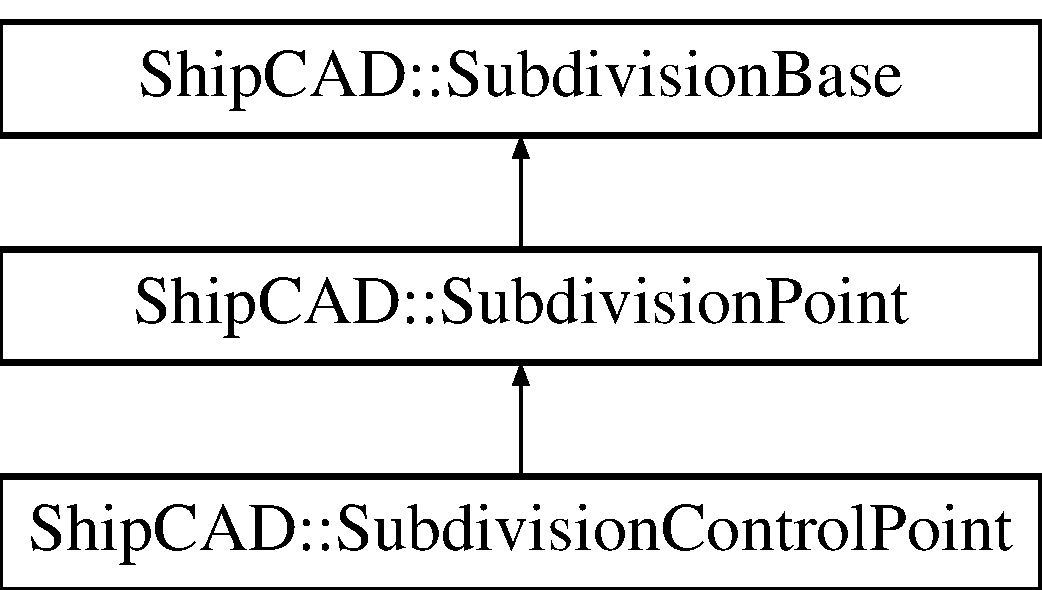
\includegraphics[height=4.000000cm]{classShipCAD_1_1SubdivisionControlPoint}
\end{center}
\end{figure}
\subsection*{Public Member Functions}
\begin{DoxyCompactItemize}
\item 
\hyperlink{classShipCAD_1_1SubdivisionControlPoint_a812f4e2343926ef41bc7104f0f7b1dd9}{Subdivision\-Control\-Point} (\hyperlink{classShipCAD_1_1SubdivisionSurface}{Subdivision\-Surface} $\ast$owner)
\begin{DoxyCompactList}\small\item\em Constructor. \end{DoxyCompactList}\item 
virtual \hyperlink{classShipCAD_1_1SubdivisionControlPoint_aed35211e2f60cd5ed1de628d732e4791}{$\sim$\-Subdivision\-Control\-Point} ()
\item 
void \hyperlink{classShipCAD_1_1SubdivisionControlPoint_a3c11cf5f0a22b44cbc8674a5d82942b0}{collapse} ()
\item 
Q\-Color \hyperlink{classShipCAD_1_1SubdivisionControlPoint_ad3af0386e8bb679a2037054ddbdb6a20}{get\-Color} ()
\item 
bool \hyperlink{classShipCAD_1_1SubdivisionControlPoint_af446fc02c7dc2e20383e741f71f4c358}{is\-Selected} ()
\item 
bool \hyperlink{classShipCAD_1_1SubdivisionControlPoint_a1d9150cdde6105519de95a94689faa51}{is\-Leak} ()
\item 
bool \hyperlink{classShipCAD_1_1SubdivisionControlPoint_ad739bf09eb693c8956101d0576736239}{is\-Visible} ()
\item 
void \hyperlink{classShipCAD_1_1SubdivisionControlPoint_a5642f57c7f17e78c27ad6edb0fdb7f65}{set\-Selected} (bool val)
\item 
bool \hyperlink{classShipCAD_1_1SubdivisionControlPoint_aacd7add9e1a79cc7e96c1ac6de568ad1}{is\-Locked} ()
\item 
void \hyperlink{classShipCAD_1_1SubdivisionControlPoint_a5f2cde3c54ca44c4b4d3ded0e3bc4ded}{set\-Locked} (bool val)
\item 
virtual size\-\_\-t \hyperlink{classShipCAD_1_1SubdivisionControlPoint_a13c569f0894ba6193a3abf894bc4b517}{get\-Index} ()
\begin{DoxyCompactList}\small\item\em index of this point in parent surface \end{DoxyCompactList}\item 
virtual void \hyperlink{classShipCAD_1_1SubdivisionControlPoint_a54a5233e02ef34a174c24d5dcf3c6407}{set\-Coordinate} (const Q\-Vector3\-D \&val)
\item 
void \hyperlink{classShipCAD_1_1SubdivisionControlPoint_a989c801ca1c836ca73f77c68d719f546}{load\-\_\-binary} (\hyperlink{classShipCAD_1_1FileBuffer}{File\-Buffer} \&source)
\item 
void \hyperlink{classShipCAD_1_1SubdivisionControlPoint_a7de1a32ae9e845478ec1bd5eaec17cd1}{save\-\_\-binary} (\hyperlink{classShipCAD_1_1FileBuffer}{File\-Buffer} \&destination)
\item 
void \hyperlink{classShipCAD_1_1SubdivisionControlPoint_a09769bfb0b63980387c23736081acdf1}{load\-From\-Stream} (size\-\_\-t \&lineno, std\-::vector$<$ Q\-String $>$ \&strings)
\item 
void \hyperlink{classShipCAD_1_1SubdivisionControlPoint_a60cc866bff57473700fbea4e17adcb4d}{save\-To\-Stream} (std\-::vector$<$ Q\-String $>$ \&strings)
\item 
virtual void \hyperlink{classShipCAD_1_1SubdivisionControlPoint_a4a9d6e45291c27f19f0d76c9b9d19048}{dump} (std\-::ostream \&os, const char $\ast$prefix=\char`\"{}\char`\"{}) const 
\begin{DoxyCompactList}\small\item\em print out the element to a stream \end{DoxyCompactList}\end{DoxyCompactItemize}
\subsection*{Static Public Member Functions}
\begin{DoxyCompactItemize}
\item 
static void \hyperlink{classShipCAD_1_1SubdivisionControlPoint_a761599371138b34be2c7a2cac3699e2c}{draw\-Control\-Points} (\hyperlink{classShipCAD_1_1Viewport}{Viewport} \&vp, \hyperlink{classShipCAD_1_1SubdivisionSurface}{Subdivision\-Surface} $\ast$surface)
\item 
static \hyperlink{classShipCAD_1_1SubdivisionControlPoint}{Subdivision\-Control\-Point} $\ast$ \hyperlink{classShipCAD_1_1SubdivisionControlPoint_adc189f3e5cff85ecd1a59356e0f7d63d}{construct} (\hyperlink{classShipCAD_1_1SubdivisionSurface}{Subdivision\-Surface} $\ast$owner)
\end{DoxyCompactItemize}
\subsection*{Protected Member Functions}
\begin{DoxyCompactItemize}
\item 
void \hyperlink{classShipCAD_1_1SubdivisionControlPoint_a01e1eff38ecb4393948db0d9883cad84}{priv\-\_\-dump} (std\-::ostream \&os, const char $\ast$prefix) const 
\end{DoxyCompactItemize}
\subsection*{Protected Attributes}
\begin{DoxyCompactItemize}
\item 
bool \hyperlink{classShipCAD_1_1SubdivisionControlPoint_acf4dc0c2a3d4c52847c68a8a412669f5}{\-\_\-locked}
\end{DoxyCompactItemize}
\subsection*{Properties}
\begin{DoxyCompactItemize}
\item 
Q\-Color \hyperlink{classShipCAD_1_1SubdivisionControlPoint_a8c7a97ce5194163f37a4b655f87bc309}{Color}
\item 
bool \hyperlink{classShipCAD_1_1SubdivisionControlPoint_af7c63177a12f4c60bb4a2a6615482a98}{Locked}
\item 
bool \hyperlink{classShipCAD_1_1SubdivisionControlPoint_a54bf97e33f121843af563f2eebe7d3e5}{Selected}
\item 
bool \hyperlink{classShipCAD_1_1SubdivisionControlPoint_ab796dbf230e01f51a1031ec69f8f7f66}{Visible}
\item 
bool \hyperlink{classShipCAD_1_1SubdivisionControlPoint_a33a15d8a83f43369313d57a854046ff7}{Is\-Leak}
\end{DoxyCompactItemize}


\subsection{Detailed Description}
Control point. 

Subdivision Surfaces consist of control points which define the surface contour 

Definition at line 209 of file subdivpoint.\-h.



\subsection{Constructor \& Destructor Documentation}
\hypertarget{classShipCAD_1_1SubdivisionControlPoint_a812f4e2343926ef41bc7104f0f7b1dd9}{\index{Ship\-C\-A\-D\-::\-Subdivision\-Control\-Point@{Ship\-C\-A\-D\-::\-Subdivision\-Control\-Point}!Subdivision\-Control\-Point@{Subdivision\-Control\-Point}}
\index{Subdivision\-Control\-Point@{Subdivision\-Control\-Point}!ShipCAD::SubdivisionControlPoint@{Ship\-C\-A\-D\-::\-Subdivision\-Control\-Point}}
\subsubsection[{Subdivision\-Control\-Point}]{\setlength{\rightskip}{0pt plus 5cm}Subdivision\-Control\-Point\-::\-Subdivision\-Control\-Point (
\begin{DoxyParamCaption}
\item[{{\bf Subdivision\-Surface} $\ast$}]{owner}
\end{DoxyParamCaption}
)\hspace{0.3cm}{\ttfamily [explicit]}}}\label{classShipCAD_1_1SubdivisionControlPoint_a812f4e2343926ef41bc7104f0f7b1dd9}


Constructor. 

New points should be created with the static construct method


\begin{DoxyParams}{Parameters}
{\em owner} & the surface this control point belongs to \\
\hline
\end{DoxyParams}


Definition at line 516 of file subdivpoint.\-cpp.

\hypertarget{classShipCAD_1_1SubdivisionControlPoint_aed35211e2f60cd5ed1de628d732e4791}{\index{Ship\-C\-A\-D\-::\-Subdivision\-Control\-Point@{Ship\-C\-A\-D\-::\-Subdivision\-Control\-Point}!$\sim$\-Subdivision\-Control\-Point@{$\sim$\-Subdivision\-Control\-Point}}
\index{$\sim$\-Subdivision\-Control\-Point@{$\sim$\-Subdivision\-Control\-Point}!ShipCAD::SubdivisionControlPoint@{Ship\-C\-A\-D\-::\-Subdivision\-Control\-Point}}
\subsubsection[{$\sim$\-Subdivision\-Control\-Point}]{\setlength{\rightskip}{0pt plus 5cm}Subdivision\-Control\-Point\-::$\sim$\-Subdivision\-Control\-Point (
\begin{DoxyParamCaption}
{}
\end{DoxyParamCaption}
)\hspace{0.3cm}{\ttfamily [virtual]}}}\label{classShipCAD_1_1SubdivisionControlPoint_aed35211e2f60cd5ed1de628d732e4791}


Definition at line 522 of file subdivpoint.\-cpp.



\subsection{Member Function Documentation}
\hypertarget{classShipCAD_1_1SubdivisionControlPoint_a3c11cf5f0a22b44cbc8674a5d82942b0}{\index{Ship\-C\-A\-D\-::\-Subdivision\-Control\-Point@{Ship\-C\-A\-D\-::\-Subdivision\-Control\-Point}!collapse@{collapse}}
\index{collapse@{collapse}!ShipCAD::SubdivisionControlPoint@{Ship\-C\-A\-D\-::\-Subdivision\-Control\-Point}}
\subsubsection[{collapse}]{\setlength{\rightskip}{0pt plus 5cm}void Subdivision\-Control\-Point\-::collapse (
\begin{DoxyParamCaption}
{}
\end{DoxyParamCaption}
)}}\label{classShipCAD_1_1SubdivisionControlPoint_a3c11cf5f0a22b44cbc8674a5d82942b0}


Definition at line 624 of file subdivpoint.\-cpp.

\hypertarget{classShipCAD_1_1SubdivisionControlPoint_adc189f3e5cff85ecd1a59356e0f7d63d}{\index{Ship\-C\-A\-D\-::\-Subdivision\-Control\-Point@{Ship\-C\-A\-D\-::\-Subdivision\-Control\-Point}!construct@{construct}}
\index{construct@{construct}!ShipCAD::SubdivisionControlPoint@{Ship\-C\-A\-D\-::\-Subdivision\-Control\-Point}}
\subsubsection[{construct}]{\setlength{\rightskip}{0pt plus 5cm}{\bf Subdivision\-Control\-Point} $\ast$ Subdivision\-Control\-Point\-::construct (
\begin{DoxyParamCaption}
\item[{{\bf Subdivision\-Surface} $\ast$}]{owner}
\end{DoxyParamCaption}
)\hspace{0.3cm}{\ttfamily [static]}}}\label{classShipCAD_1_1SubdivisionControlPoint_adc189f3e5cff85ecd1a59356e0f7d63d}


Definition at line 508 of file subdivpoint.\-cpp.

\hypertarget{classShipCAD_1_1SubdivisionControlPoint_a761599371138b34be2c7a2cac3699e2c}{\index{Ship\-C\-A\-D\-::\-Subdivision\-Control\-Point@{Ship\-C\-A\-D\-::\-Subdivision\-Control\-Point}!draw\-Control\-Points@{draw\-Control\-Points}}
\index{draw\-Control\-Points@{draw\-Control\-Points}!ShipCAD::SubdivisionControlPoint@{Ship\-C\-A\-D\-::\-Subdivision\-Control\-Point}}
\subsubsection[{draw\-Control\-Points}]{\setlength{\rightskip}{0pt plus 5cm}void Subdivision\-Control\-Point\-::draw\-Control\-Points (
\begin{DoxyParamCaption}
\item[{{\bf Viewport} \&}]{vp, }
\item[{{\bf Subdivision\-Surface} $\ast$}]{surface}
\end{DoxyParamCaption}
)\hspace{0.3cm}{\ttfamily [static]}}}\label{classShipCAD_1_1SubdivisionControlPoint_a761599371138b34be2c7a2cac3699e2c}


Definition at line 817 of file subdivpoint.\-cpp.

\hypertarget{classShipCAD_1_1SubdivisionControlPoint_a4a9d6e45291c27f19f0d76c9b9d19048}{\index{Ship\-C\-A\-D\-::\-Subdivision\-Control\-Point@{Ship\-C\-A\-D\-::\-Subdivision\-Control\-Point}!dump@{dump}}
\index{dump@{dump}!ShipCAD::SubdivisionControlPoint@{Ship\-C\-A\-D\-::\-Subdivision\-Control\-Point}}
\subsubsection[{dump}]{\setlength{\rightskip}{0pt plus 5cm}void Subdivision\-Control\-Point\-::dump (
\begin{DoxyParamCaption}
\item[{std\-::ostream \&}]{os, }
\item[{const char $\ast$}]{prefix = {\ttfamily \char`\"{}\char`\"{}}}
\end{DoxyParamCaption}
) const\hspace{0.3cm}{\ttfamily [virtual]}}}\label{classShipCAD_1_1SubdivisionControlPoint_a4a9d6e45291c27f19f0d76c9b9d19048}


print out the element to a stream 


\begin{DoxyParams}{Parameters}
{\em os} & the output stream \\
\hline
{\em prefix} & string to prefix on each line output \\
\hline
\end{DoxyParams}


Reimplemented from \hyperlink{classShipCAD_1_1SubdivisionPoint_aed72cf5e8dc67e980010d195f3a376a3}{Ship\-C\-A\-D\-::\-Subdivision\-Point}.



Definition at line 877 of file subdivpoint.\-cpp.

\hypertarget{classShipCAD_1_1SubdivisionControlPoint_ad3af0386e8bb679a2037054ddbdb6a20}{\index{Ship\-C\-A\-D\-::\-Subdivision\-Control\-Point@{Ship\-C\-A\-D\-::\-Subdivision\-Control\-Point}!get\-Color@{get\-Color}}
\index{get\-Color@{get\-Color}!ShipCAD::SubdivisionControlPoint@{Ship\-C\-A\-D\-::\-Subdivision\-Control\-Point}}
\subsubsection[{get\-Color}]{\setlength{\rightskip}{0pt plus 5cm}Q\-Color Subdivision\-Control\-Point\-::get\-Color (
\begin{DoxyParamCaption}
{}
\end{DoxyParamCaption}
)}}\label{classShipCAD_1_1SubdivisionControlPoint_ad3af0386e8bb679a2037054ddbdb6a20}


Definition at line 529 of file subdivpoint.\-cpp.

\hypertarget{classShipCAD_1_1SubdivisionControlPoint_a13c569f0894ba6193a3abf894bc4b517}{\index{Ship\-C\-A\-D\-::\-Subdivision\-Control\-Point@{Ship\-C\-A\-D\-::\-Subdivision\-Control\-Point}!get\-Index@{get\-Index}}
\index{get\-Index@{get\-Index}!ShipCAD::SubdivisionControlPoint@{Ship\-C\-A\-D\-::\-Subdivision\-Control\-Point}}
\subsubsection[{get\-Index}]{\setlength{\rightskip}{0pt plus 5cm}size\-\_\-t Subdivision\-Control\-Point\-::get\-Index (
\begin{DoxyParamCaption}
{}
\end{DoxyParamCaption}
)\hspace{0.3cm}{\ttfamily [virtual]}}}\label{classShipCAD_1_1SubdivisionControlPoint_a13c569f0894ba6193a3abf894bc4b517}


index of this point in parent surface 

\begin{DoxyReturn}{Returns}
the index of this point in parent surface 
\end{DoxyReturn}


Reimplemented from \hyperlink{classShipCAD_1_1SubdivisionPoint_a8406682549c10ec9e1a184132f6ed2f0}{Ship\-C\-A\-D\-::\-Subdivision\-Point}.



Definition at line 551 of file subdivpoint.\-cpp.

\hypertarget{classShipCAD_1_1SubdivisionControlPoint_a1d9150cdde6105519de95a94689faa51}{\index{Ship\-C\-A\-D\-::\-Subdivision\-Control\-Point@{Ship\-C\-A\-D\-::\-Subdivision\-Control\-Point}!is\-Leak@{is\-Leak}}
\index{is\-Leak@{is\-Leak}!ShipCAD::SubdivisionControlPoint@{Ship\-C\-A\-D\-::\-Subdivision\-Control\-Point}}
\subsubsection[{is\-Leak}]{\setlength{\rightskip}{0pt plus 5cm}bool Subdivision\-Control\-Point\-::is\-Leak (
\begin{DoxyParamCaption}
{}
\end{DoxyParamCaption}
)}}\label{classShipCAD_1_1SubdivisionControlPoint_a1d9150cdde6105519de95a94689faa51}


Definition at line 595 of file subdivpoint.\-cpp.

\hypertarget{classShipCAD_1_1SubdivisionControlPoint_aacd7add9e1a79cc7e96c1ac6de568ad1}{\index{Ship\-C\-A\-D\-::\-Subdivision\-Control\-Point@{Ship\-C\-A\-D\-::\-Subdivision\-Control\-Point}!is\-Locked@{is\-Locked}}
\index{is\-Locked@{is\-Locked}!ShipCAD::SubdivisionControlPoint@{Ship\-C\-A\-D\-::\-Subdivision\-Control\-Point}}
\subsubsection[{is\-Locked}]{\setlength{\rightskip}{0pt plus 5cm}bool Ship\-C\-A\-D\-::\-Subdivision\-Control\-Point\-::is\-Locked (
\begin{DoxyParamCaption}
{}
\end{DoxyParamCaption}
)\hspace{0.3cm}{\ttfamily [inline]}}}\label{classShipCAD_1_1SubdivisionControlPoint_aacd7add9e1a79cc7e96c1ac6de568ad1}


Definition at line 237 of file subdivpoint.\-h.

\hypertarget{classShipCAD_1_1SubdivisionControlPoint_af446fc02c7dc2e20383e741f71f4c358}{\index{Ship\-C\-A\-D\-::\-Subdivision\-Control\-Point@{Ship\-C\-A\-D\-::\-Subdivision\-Control\-Point}!is\-Selected@{is\-Selected}}
\index{is\-Selected@{is\-Selected}!ShipCAD::SubdivisionControlPoint@{Ship\-C\-A\-D\-::\-Subdivision\-Control\-Point}}
\subsubsection[{is\-Selected}]{\setlength{\rightskip}{0pt plus 5cm}bool Subdivision\-Control\-Point\-::is\-Selected (
\begin{DoxyParamCaption}
{}
\end{DoxyParamCaption}
)}}\label{classShipCAD_1_1SubdivisionControlPoint_af446fc02c7dc2e20383e741f71f4c358}


Definition at line 556 of file subdivpoint.\-cpp.

\hypertarget{classShipCAD_1_1SubdivisionControlPoint_ad739bf09eb693c8956101d0576736239}{\index{Ship\-C\-A\-D\-::\-Subdivision\-Control\-Point@{Ship\-C\-A\-D\-::\-Subdivision\-Control\-Point}!is\-Visible@{is\-Visible}}
\index{is\-Visible@{is\-Visible}!ShipCAD::SubdivisionControlPoint@{Ship\-C\-A\-D\-::\-Subdivision\-Control\-Point}}
\subsubsection[{is\-Visible}]{\setlength{\rightskip}{0pt plus 5cm}bool Subdivision\-Control\-Point\-::is\-Visible (
\begin{DoxyParamCaption}
{}
\end{DoxyParamCaption}
)}}\label{classShipCAD_1_1SubdivisionControlPoint_ad739bf09eb693c8956101d0576736239}


Definition at line 561 of file subdivpoint.\-cpp.

\hypertarget{classShipCAD_1_1SubdivisionControlPoint_a989c801ca1c836ca73f77c68d719f546}{\index{Ship\-C\-A\-D\-::\-Subdivision\-Control\-Point@{Ship\-C\-A\-D\-::\-Subdivision\-Control\-Point}!load\-\_\-binary@{load\-\_\-binary}}
\index{load\-\_\-binary@{load\-\_\-binary}!ShipCAD::SubdivisionControlPoint@{Ship\-C\-A\-D\-::\-Subdivision\-Control\-Point}}
\subsubsection[{load\-\_\-binary}]{\setlength{\rightskip}{0pt plus 5cm}void Subdivision\-Control\-Point\-::load\-\_\-binary (
\begin{DoxyParamCaption}
\item[{{\bf File\-Buffer} \&}]{source}
\end{DoxyParamCaption}
)}}\label{classShipCAD_1_1SubdivisionControlPoint_a989c801ca1c836ca73f77c68d719f546}


Definition at line 761 of file subdivpoint.\-cpp.

\hypertarget{classShipCAD_1_1SubdivisionControlPoint_a09769bfb0b63980387c23736081acdf1}{\index{Ship\-C\-A\-D\-::\-Subdivision\-Control\-Point@{Ship\-C\-A\-D\-::\-Subdivision\-Control\-Point}!load\-From\-Stream@{load\-From\-Stream}}
\index{load\-From\-Stream@{load\-From\-Stream}!ShipCAD::SubdivisionControlPoint@{Ship\-C\-A\-D\-::\-Subdivision\-Control\-Point}}
\subsubsection[{load\-From\-Stream}]{\setlength{\rightskip}{0pt plus 5cm}void Subdivision\-Control\-Point\-::load\-From\-Stream (
\begin{DoxyParamCaption}
\item[{size\-\_\-t \&}]{lineno, }
\item[{std\-::vector$<$ Q\-String $>$ \&}]{strings}
\end{DoxyParamCaption}
)}}\label{classShipCAD_1_1SubdivisionControlPoint_a09769bfb0b63980387c23736081acdf1}


Definition at line 775 of file subdivpoint.\-cpp.

\hypertarget{classShipCAD_1_1SubdivisionControlPoint_a01e1eff38ecb4393948db0d9883cad84}{\index{Ship\-C\-A\-D\-::\-Subdivision\-Control\-Point@{Ship\-C\-A\-D\-::\-Subdivision\-Control\-Point}!priv\-\_\-dump@{priv\-\_\-dump}}
\index{priv\-\_\-dump@{priv\-\_\-dump}!ShipCAD::SubdivisionControlPoint@{Ship\-C\-A\-D\-::\-Subdivision\-Control\-Point}}
\subsubsection[{priv\-\_\-dump}]{\setlength{\rightskip}{0pt plus 5cm}void Subdivision\-Control\-Point\-::priv\-\_\-dump (
\begin{DoxyParamCaption}
\item[{std\-::ostream \&}]{os, }
\item[{const char $\ast$}]{prefix}
\end{DoxyParamCaption}
) const\hspace{0.3cm}{\ttfamily [protected]}}}\label{classShipCAD_1_1SubdivisionControlPoint_a01e1eff38ecb4393948db0d9883cad84}


Definition at line 885 of file subdivpoint.\-cpp.

\hypertarget{classShipCAD_1_1SubdivisionControlPoint_a7de1a32ae9e845478ec1bd5eaec17cd1}{\index{Ship\-C\-A\-D\-::\-Subdivision\-Control\-Point@{Ship\-C\-A\-D\-::\-Subdivision\-Control\-Point}!save\-\_\-binary@{save\-\_\-binary}}
\index{save\-\_\-binary@{save\-\_\-binary}!ShipCAD::SubdivisionControlPoint@{Ship\-C\-A\-D\-::\-Subdivision\-Control\-Point}}
\subsubsection[{save\-\_\-binary}]{\setlength{\rightskip}{0pt plus 5cm}void Subdivision\-Control\-Point\-::save\-\_\-binary (
\begin{DoxyParamCaption}
\item[{{\bf File\-Buffer} \&}]{destination}
\end{DoxyParamCaption}
)}}\label{classShipCAD_1_1SubdivisionControlPoint_a7de1a32ae9e845478ec1bd5eaec17cd1}


Definition at line 808 of file subdivpoint.\-cpp.

\hypertarget{classShipCAD_1_1SubdivisionControlPoint_a60cc866bff57473700fbea4e17adcb4d}{\index{Ship\-C\-A\-D\-::\-Subdivision\-Control\-Point@{Ship\-C\-A\-D\-::\-Subdivision\-Control\-Point}!save\-To\-Stream@{save\-To\-Stream}}
\index{save\-To\-Stream@{save\-To\-Stream}!ShipCAD::SubdivisionControlPoint@{Ship\-C\-A\-D\-::\-Subdivision\-Control\-Point}}
\subsubsection[{save\-To\-Stream}]{\setlength{\rightskip}{0pt plus 5cm}void Subdivision\-Control\-Point\-::save\-To\-Stream (
\begin{DoxyParamCaption}
\item[{std\-::vector$<$ Q\-String $>$ \&}]{strings}
\end{DoxyParamCaption}
)}}\label{classShipCAD_1_1SubdivisionControlPoint_a60cc866bff57473700fbea4e17adcb4d}


Definition at line 797 of file subdivpoint.\-cpp.

\hypertarget{classShipCAD_1_1SubdivisionControlPoint_a54a5233e02ef34a174c24d5dcf3c6407}{\index{Ship\-C\-A\-D\-::\-Subdivision\-Control\-Point@{Ship\-C\-A\-D\-::\-Subdivision\-Control\-Point}!set\-Coordinate@{set\-Coordinate}}
\index{set\-Coordinate@{set\-Coordinate}!ShipCAD::SubdivisionControlPoint@{Ship\-C\-A\-D\-::\-Subdivision\-Control\-Point}}
\subsubsection[{set\-Coordinate}]{\setlength{\rightskip}{0pt plus 5cm}void Subdivision\-Control\-Point\-::set\-Coordinate (
\begin{DoxyParamCaption}
\item[{const Q\-Vector3\-D \&}]{val}
\end{DoxyParamCaption}
)\hspace{0.3cm}{\ttfamily [virtual]}}}\label{classShipCAD_1_1SubdivisionControlPoint_a54a5233e02ef34a174c24d5dcf3c6407}


Reimplemented from \hyperlink{classShipCAD_1_1SubdivisionPoint_a98ab99a0ccc4709a40e05b36147c0f55}{Ship\-C\-A\-D\-::\-Subdivision\-Point}.



Definition at line 618 of file subdivpoint.\-cpp.

\hypertarget{classShipCAD_1_1SubdivisionControlPoint_a5f2cde3c54ca44c4b4d3ded0e3bc4ded}{\index{Ship\-C\-A\-D\-::\-Subdivision\-Control\-Point@{Ship\-C\-A\-D\-::\-Subdivision\-Control\-Point}!set\-Locked@{set\-Locked}}
\index{set\-Locked@{set\-Locked}!ShipCAD::SubdivisionControlPoint@{Ship\-C\-A\-D\-::\-Subdivision\-Control\-Point}}
\subsubsection[{set\-Locked}]{\setlength{\rightskip}{0pt plus 5cm}void Subdivision\-Control\-Point\-::set\-Locked (
\begin{DoxyParamCaption}
\item[{bool}]{val}
\end{DoxyParamCaption}
)}}\label{classShipCAD_1_1SubdivisionControlPoint_a5f2cde3c54ca44c4b4d3ded0e3bc4ded}


Definition at line 612 of file subdivpoint.\-cpp.

\hypertarget{classShipCAD_1_1SubdivisionControlPoint_a5642f57c7f17e78c27ad6edb0fdb7f65}{\index{Ship\-C\-A\-D\-::\-Subdivision\-Control\-Point@{Ship\-C\-A\-D\-::\-Subdivision\-Control\-Point}!set\-Selected@{set\-Selected}}
\index{set\-Selected@{set\-Selected}!ShipCAD::SubdivisionControlPoint@{Ship\-C\-A\-D\-::\-Subdivision\-Control\-Point}}
\subsubsection[{set\-Selected}]{\setlength{\rightskip}{0pt plus 5cm}void Subdivision\-Control\-Point\-::set\-Selected (
\begin{DoxyParamCaption}
\item[{bool}]{val}
\end{DoxyParamCaption}
)}}\label{classShipCAD_1_1SubdivisionControlPoint_a5642f57c7f17e78c27ad6edb0fdb7f65}


Definition at line 600 of file subdivpoint.\-cpp.



\subsection{Member Data Documentation}
\hypertarget{classShipCAD_1_1SubdivisionControlPoint_acf4dc0c2a3d4c52847c68a8a412669f5}{\index{Ship\-C\-A\-D\-::\-Subdivision\-Control\-Point@{Ship\-C\-A\-D\-::\-Subdivision\-Control\-Point}!\-\_\-locked@{\-\_\-locked}}
\index{\-\_\-locked@{\-\_\-locked}!ShipCAD::SubdivisionControlPoint@{Ship\-C\-A\-D\-::\-Subdivision\-Control\-Point}}
\subsubsection[{\-\_\-locked}]{\setlength{\rightskip}{0pt plus 5cm}bool Ship\-C\-A\-D\-::\-Subdivision\-Control\-Point\-::\-\_\-locked\hspace{0.3cm}{\ttfamily [protected]}}}\label{classShipCAD_1_1SubdivisionControlPoint_acf4dc0c2a3d4c52847c68a8a412669f5}
whether point is locked 

Definition at line 267 of file subdivpoint.\-h.



\subsection{Property Documentation}
\hypertarget{classShipCAD_1_1SubdivisionControlPoint_a8c7a97ce5194163f37a4b655f87bc309}{\index{Ship\-C\-A\-D\-::\-Subdivision\-Control\-Point@{Ship\-C\-A\-D\-::\-Subdivision\-Control\-Point}!Color@{Color}}
\index{Color@{Color}!ShipCAD::SubdivisionControlPoint@{Ship\-C\-A\-D\-::\-Subdivision\-Control\-Point}}
\subsubsection[{Color}]{\setlength{\rightskip}{0pt plus 5cm}Q\-Color Ship\-C\-A\-D\-::\-Subdivision\-Control\-Point\-::\-Color\hspace{0.3cm}{\ttfamily [read]}}}\label{classShipCAD_1_1SubdivisionControlPoint_a8c7a97ce5194163f37a4b655f87bc309}


Definition at line 212 of file subdivpoint.\-h.

\hypertarget{classShipCAD_1_1SubdivisionControlPoint_a33a15d8a83f43369313d57a854046ff7}{\index{Ship\-C\-A\-D\-::\-Subdivision\-Control\-Point@{Ship\-C\-A\-D\-::\-Subdivision\-Control\-Point}!Is\-Leak@{Is\-Leak}}
\index{Is\-Leak@{Is\-Leak}!ShipCAD::SubdivisionControlPoint@{Ship\-C\-A\-D\-::\-Subdivision\-Control\-Point}}
\subsubsection[{Is\-Leak}]{\setlength{\rightskip}{0pt plus 5cm}bool Ship\-C\-A\-D\-::\-Subdivision\-Control\-Point\-::\-Is\-Leak\hspace{0.3cm}{\ttfamily [read]}}}\label{classShipCAD_1_1SubdivisionControlPoint_a33a15d8a83f43369313d57a854046ff7}


Definition at line 216 of file subdivpoint.\-h.

\hypertarget{classShipCAD_1_1SubdivisionControlPoint_af7c63177a12f4c60bb4a2a6615482a98}{\index{Ship\-C\-A\-D\-::\-Subdivision\-Control\-Point@{Ship\-C\-A\-D\-::\-Subdivision\-Control\-Point}!Locked@{Locked}}
\index{Locked@{Locked}!ShipCAD::SubdivisionControlPoint@{Ship\-C\-A\-D\-::\-Subdivision\-Control\-Point}}
\subsubsection[{Locked}]{\setlength{\rightskip}{0pt plus 5cm}bool Ship\-C\-A\-D\-::\-Subdivision\-Control\-Point\-::\-Locked\hspace{0.3cm}{\ttfamily [read]}, {\ttfamily [write]}}}\label{classShipCAD_1_1SubdivisionControlPoint_af7c63177a12f4c60bb4a2a6615482a98}


Definition at line 213 of file subdivpoint.\-h.

\hypertarget{classShipCAD_1_1SubdivisionControlPoint_a54bf97e33f121843af563f2eebe7d3e5}{\index{Ship\-C\-A\-D\-::\-Subdivision\-Control\-Point@{Ship\-C\-A\-D\-::\-Subdivision\-Control\-Point}!Selected@{Selected}}
\index{Selected@{Selected}!ShipCAD::SubdivisionControlPoint@{Ship\-C\-A\-D\-::\-Subdivision\-Control\-Point}}
\subsubsection[{Selected}]{\setlength{\rightskip}{0pt plus 5cm}bool Ship\-C\-A\-D\-::\-Subdivision\-Control\-Point\-::\-Selected\hspace{0.3cm}{\ttfamily [read]}, {\ttfamily [write]}}}\label{classShipCAD_1_1SubdivisionControlPoint_a54bf97e33f121843af563f2eebe7d3e5}


Definition at line 214 of file subdivpoint.\-h.

\hypertarget{classShipCAD_1_1SubdivisionControlPoint_ab796dbf230e01f51a1031ec69f8f7f66}{\index{Ship\-C\-A\-D\-::\-Subdivision\-Control\-Point@{Ship\-C\-A\-D\-::\-Subdivision\-Control\-Point}!Visible@{Visible}}
\index{Visible@{Visible}!ShipCAD::SubdivisionControlPoint@{Ship\-C\-A\-D\-::\-Subdivision\-Control\-Point}}
\subsubsection[{Visible}]{\setlength{\rightskip}{0pt plus 5cm}bool Ship\-C\-A\-D\-::\-Subdivision\-Control\-Point\-::\-Visible\hspace{0.3cm}{\ttfamily [read]}}}\label{classShipCAD_1_1SubdivisionControlPoint_ab796dbf230e01f51a1031ec69f8f7f66}


Definition at line 215 of file subdivpoint.\-h.



The documentation for this class was generated from the following files\-:\begin{DoxyCompactItemize}
\item 
Ship\-C\-A\-Dlib/\hyperlink{subdivpoint_8h}{subdivpoint.\-h}\item 
Ship\-C\-A\-Dlib/\hyperlink{subdivpoint_8cpp}{subdivpoint.\-cpp}\end{DoxyCompactItemize}

\hypertarget{classShipCAD_1_1SubdivisionEdge}{\section{Ship\-C\-A\-D\-:\-:Subdivision\-Edge Class Reference}
\label{classShipCAD_1_1SubdivisionEdge}\index{Ship\-C\-A\-D\-::\-Subdivision\-Edge@{Ship\-C\-A\-D\-::\-Subdivision\-Edge}}
}


{\ttfamily \#include $<$subdivedge.\-h$>$}

Inheritance diagram for Ship\-C\-A\-D\-:\-:Subdivision\-Edge\-:\begin{figure}[H]
\begin{center}
\leavevmode
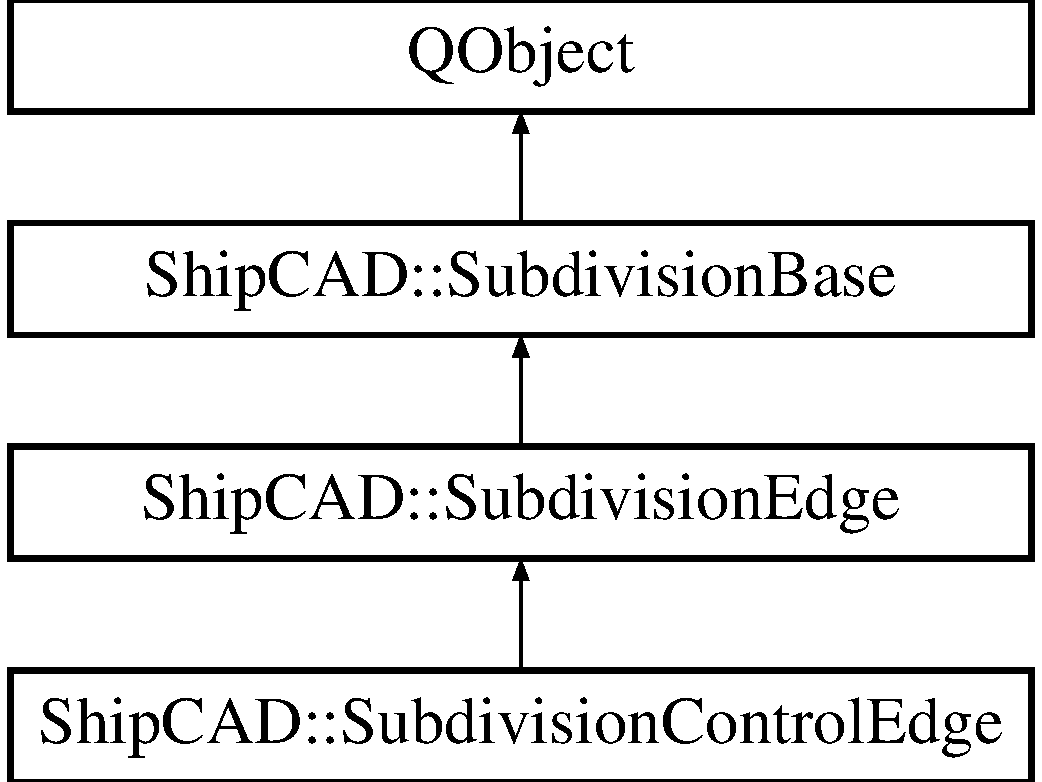
\includegraphics[height=4.000000cm]{classShipCAD_1_1SubdivisionEdge}
\end{center}
\end{figure}
\subsection*{Public Member Functions}
\begin{DoxyCompactItemize}
\item 
\hyperlink{classShipCAD_1_1SubdivisionEdge_ab08271ed7f5d371f0495d8a7d2c96dae}{Subdivision\-Edge} (\hyperlink{classShipCAD_1_1SubdivisionSurface}{Subdivision\-Surface} $\ast$owner)
\item 
virtual \hyperlink{classShipCAD_1_1SubdivisionEdge_ac787ad1a0228f91038de9518ad217364}{$\sim$\-Subdivision\-Edge} ()
\item 
virtual void \hyperlink{classShipCAD_1_1SubdivisionEdge_a08358ac65c2d710855b8b93c64ce9d02}{clear} ()
\begin{DoxyCompactList}\small\item\em reset this element to default values \end{DoxyCompactList}\item 
virtual void \hyperlink{classShipCAD_1_1SubdivisionEdge_a26deda12672fa679b49b28f2371e728b}{draw} (bool draw\-\_\-mirror, \hyperlink{classShipCAD_1_1Viewport}{Viewport} \&vp, \hyperlink{classShipCAD_1_1LineShader}{Line\-Shader} $\ast$lineshader, const Q\-Color \&edge\-Color)
\item 
void \hyperlink{classShipCAD_1_1SubdivisionEdge_a1b2e2b1d7e051d42250c0ad1f5eaa560}{add\-Face} (\hyperlink{classShipCAD_1_1SubdivisionFace}{Subdivision\-Face} $\ast$face)
\item 
void \hyperlink{classShipCAD_1_1SubdivisionEdge_a847a6c74d35e25fdcb46ea8b7a989836}{assign} (\hyperlink{classShipCAD_1_1SubdivisionEdge}{Subdivision\-Edge} $\ast$edge)
\item 
\hyperlink{classShipCAD_1_1SubdivisionPoint}{Subdivision\-Point} $\ast$ \hyperlink{classShipCAD_1_1SubdivisionEdge_aa1bce1c13f4911839205e812cfd0f683}{calculate\-Edge\-Point} ()
\item 
void \hyperlink{classShipCAD_1_1SubdivisionEdge_a1f4b70ab6d0c4dfec07a2d4348bc9a3e}{delete\-Face} (\hyperlink{classShipCAD_1_1SubdivisionFace}{Subdivision\-Face} $\ast$face)
\item 
void \hyperlink{classShipCAD_1_1SubdivisionEdge_ad19ddea08367fa2307e131132e36c008}{swap\-Data} ()
\item 
\hyperlink{classShipCAD_1_1SubdivisionPoint}{Subdivision\-Point} $\ast$ \hyperlink{classShipCAD_1_1SubdivisionEdge_a63a44ac44fe9d2729e5152303b249873}{start\-Point} ()
\item 
\hyperlink{classShipCAD_1_1SubdivisionPoint}{Subdivision\-Point} $\ast$ \hyperlink{classShipCAD_1_1SubdivisionEdge_a69acb7c9d026f05ea727fd80dc7ab6a0}{end\-Point} ()
\item 
virtual bool \hyperlink{classShipCAD_1_1SubdivisionEdge_ad95a3ec8ba66deb74cbfd3d36428fc34}{is\-Boundary\-Edge} ()
\item 
bool \hyperlink{classShipCAD_1_1SubdivisionEdge_a697962345138e27e520e3da8e3f2289a}{is\-Control\-Edge} ()
\item 
void \hyperlink{classShipCAD_1_1SubdivisionEdge_af48a9311daf8f3607e181922162e8c7b}{set\-Control\-Edge} (bool val)
\item 
size\-\_\-t \hyperlink{classShipCAD_1_1SubdivisionEdge_ae42291f7c6f7e6bdb647f27b8b0aa08e}{number\-Of\-Faces} ()
\item 
bool \hyperlink{classShipCAD_1_1SubdivisionEdge_a8bd402a4e395de86fb0095e72b91cfc4}{is\-Crease} ()
\item 
void \hyperlink{classShipCAD_1_1SubdivisionEdge_ad0313b8844a81c5802533376a09fce99}{set\-Crease} (bool val)
\item 
\hyperlink{classShipCAD_1_1SubdivisionControlCurve}{Subdivision\-Control\-Curve} $\ast$ \hyperlink{classShipCAD_1_1SubdivisionEdge_a659dd94b180681665d991db481a0cbc6}{get\-Curve} ()
\item 
void \hyperlink{classShipCAD_1_1SubdivisionEdge_a445c08836100060818c129ea7c694234}{set\-Curve} (\hyperlink{classShipCAD_1_1SubdivisionControlCurve}{Subdivision\-Control\-Curve} $\ast$curve)
\item 
size\-\_\-t \hyperlink{classShipCAD_1_1SubdivisionEdge_a4be990243bb29ead43c76171197130d5}{get\-Index} ()
\item 
\hyperlink{classShipCAD_1_1SubdivisionFace}{Subdivision\-Face} $\ast$ \hyperlink{classShipCAD_1_1SubdivisionEdge_a55dc9daab165567ed40e37f9e01ee766}{get\-Face} (size\-\_\-t index)
\item 
bool \hyperlink{classShipCAD_1_1SubdivisionEdge_a286bc4d7959703a153945e3bcb9c9ad3}{has\-Face} (\hyperlink{classShipCAD_1_1SubdivisionFace}{Subdivision\-Face} $\ast$face)
\item 
\hyperlink{classShipCAD_1_1SubdivisionEdge}{Subdivision\-Edge} $\ast$ \hyperlink{classShipCAD_1_1SubdivisionEdge_a7c1fe2cad6e7b8a0e532768b4a395137}{get\-Previous\-Edge} ()
\item 
\hyperlink{classShipCAD_1_1SubdivisionEdge}{Subdivision\-Edge} $\ast$ \hyperlink{classShipCAD_1_1SubdivisionEdge_aebb50514ff119a1484f7c7505a527a2b}{get\-Next\-Edge} ()
\item 
void \hyperlink{classShipCAD_1_1SubdivisionEdge_ab86e4ccfa750684432c228ea2cc991ff}{set\-Points} (\hyperlink{classShipCAD_1_1SubdivisionPoint}{Subdivision\-Point} $\ast$p1, \hyperlink{classShipCAD_1_1SubdivisionPoint}{Subdivision\-Point} $\ast$p2)
\item 
virtual void \hyperlink{classShipCAD_1_1SubdivisionEdge_a14cc58877644ebd7b7ebffbdf8ef87f7}{dump} (std\-::ostream \&os, const char $\ast$prefix=\char`\"{}\char`\"{}) const 
\begin{DoxyCompactList}\small\item\em print out the element to a stream \end{DoxyCompactList}\end{DoxyCompactItemize}
\subsection*{Static Public Member Functions}
\begin{DoxyCompactItemize}
\item 
static \hyperlink{classShipCAD_1_1SubdivisionEdge}{Subdivision\-Edge} $\ast$ \hyperlink{classShipCAD_1_1SubdivisionEdge_ac2e94f4689d724a1d5b75c7f2619c37d}{construct} (\hyperlink{classShipCAD_1_1SubdivisionSurface}{Subdivision\-Surface} $\ast$owner)
\end{DoxyCompactItemize}
\subsection*{Protected Member Functions}
\begin{DoxyCompactItemize}
\item 
void \hyperlink{classShipCAD_1_1SubdivisionEdge_a8b33f4ae9edbd8ac4a386d9f5f5c1131}{priv\-\_\-dump} (std\-::ostream \&os, const char $\ast$prefix) const 
\end{DoxyCompactItemize}
\subsection*{Protected Attributes}
\begin{DoxyCompactItemize}
\item 
\hyperlink{classShipCAD_1_1SubdivisionPoint}{Subdivision\-Point} $\ast$ \hyperlink{classShipCAD_1_1SubdivisionEdge_a55519f9d615d6bd701c10c48259525ac}{\-\_\-points} \mbox{[}2\mbox{]}
\item 
std\-::vector$<$ \hyperlink{classShipCAD_1_1SubdivisionFace}{Subdivision\-Face} $\ast$ $>$ \hyperlink{classShipCAD_1_1SubdivisionEdge_aa1da730fcb3ac49c92e803a0b336d855}{\-\_\-faces}
\item 
bool \hyperlink{classShipCAD_1_1SubdivisionEdge_a9ea4714611e4970cf5e4014304a20190}{\-\_\-crease}
\item 
bool \hyperlink{classShipCAD_1_1SubdivisionEdge_ae933ee4901a7964ca50a83edad44e8ec}{\-\_\-control\-\_\-edge}
\item 
\hyperlink{classShipCAD_1_1SubdivisionControlCurve}{Subdivision\-Control\-Curve} $\ast$ \hyperlink{classShipCAD_1_1SubdivisionEdge_a1863a7ef84b2d73f0e1407f3536bbc9f}{\-\_\-curve}
\end{DoxyCompactItemize}
\subsection*{Properties}
\begin{DoxyCompactItemize}
\item 
\hyperlink{classShipCAD_1_1SubdivisionPoint}{Subdivision\-Point} \hyperlink{classShipCAD_1_1SubdivisionEdge_aa23b3f03ef499cfbd896c21987ad39b4}{Start\-Point}
\item 
\hyperlink{classShipCAD_1_1SubdivisionPoint}{Subdivision\-Point} \hyperlink{classShipCAD_1_1SubdivisionEdge_ae9b9ffdb1e43bf851e5545f7d7a1849d}{End\-Point}
\item 
bool \hyperlink{classShipCAD_1_1SubdivisionEdge_ae4e748e28975f806703ffbd458bb66a2}{Crease}
\item 
size\-\_\-t \hyperlink{classShipCAD_1_1SubdivisionEdge_ae683b98a87c34941bc550fe36666e184}{Index}
\item 
\hyperlink{classShipCAD_1_1SubdivisionControlCurve}{Subdivision\-Control\-Curve} \hyperlink{classShipCAD_1_1SubdivisionEdge_af7e2dfad80e8f8dce7a7159c3b18949c}{Curve}
\item 
bool \hyperlink{classShipCAD_1_1SubdivisionEdge_a9543fdb35c1b51844207ebcfeb743197}{Control\-Edge}
\end{DoxyCompactItemize}


\subsection{Detailed Description}


Definition at line 54 of file subdivedge.\-h.



\subsection{Constructor \& Destructor Documentation}
\hypertarget{classShipCAD_1_1SubdivisionEdge_ab08271ed7f5d371f0495d8a7d2c96dae}{\index{Ship\-C\-A\-D\-::\-Subdivision\-Edge@{Ship\-C\-A\-D\-::\-Subdivision\-Edge}!Subdivision\-Edge@{Subdivision\-Edge}}
\index{Subdivision\-Edge@{Subdivision\-Edge}!ShipCAD::SubdivisionEdge@{Ship\-C\-A\-D\-::\-Subdivision\-Edge}}
\subsubsection[{Subdivision\-Edge}]{\setlength{\rightskip}{0pt plus 5cm}Subdivision\-Edge\-::\-Subdivision\-Edge (
\begin{DoxyParamCaption}
\item[{{\bf Subdivision\-Surface} $\ast$}]{owner}
\end{DoxyParamCaption}
)\hspace{0.3cm}{\ttfamily [explicit]}}}\label{classShipCAD_1_1SubdivisionEdge_ab08271ed7f5d371f0495d8a7d2c96dae}


Definition at line 61 of file subdivedge.\-cpp.

\hypertarget{classShipCAD_1_1SubdivisionEdge_ac787ad1a0228f91038de9518ad217364}{\index{Ship\-C\-A\-D\-::\-Subdivision\-Edge@{Ship\-C\-A\-D\-::\-Subdivision\-Edge}!$\sim$\-Subdivision\-Edge@{$\sim$\-Subdivision\-Edge}}
\index{$\sim$\-Subdivision\-Edge@{$\sim$\-Subdivision\-Edge}!ShipCAD::SubdivisionEdge@{Ship\-C\-A\-D\-::\-Subdivision\-Edge}}
\subsubsection[{$\sim$\-Subdivision\-Edge}]{\setlength{\rightskip}{0pt plus 5cm}Subdivision\-Edge\-::$\sim$\-Subdivision\-Edge (
\begin{DoxyParamCaption}
{}
\end{DoxyParamCaption}
)\hspace{0.3cm}{\ttfamily [virtual]}}}\label{classShipCAD_1_1SubdivisionEdge_ac787ad1a0228f91038de9518ad217364}


Definition at line 67 of file subdivedge.\-cpp.



\subsection{Member Function Documentation}
\hypertarget{classShipCAD_1_1SubdivisionEdge_a1b2e2b1d7e051d42250c0ad1f5eaa560}{\index{Ship\-C\-A\-D\-::\-Subdivision\-Edge@{Ship\-C\-A\-D\-::\-Subdivision\-Edge}!add\-Face@{add\-Face}}
\index{add\-Face@{add\-Face}!ShipCAD::SubdivisionEdge@{Ship\-C\-A\-D\-::\-Subdivision\-Edge}}
\subsubsection[{add\-Face}]{\setlength{\rightskip}{0pt plus 5cm}void Subdivision\-Edge\-::add\-Face (
\begin{DoxyParamCaption}
\item[{{\bf Subdivision\-Face} $\ast$}]{face}
\end{DoxyParamCaption}
)}}\label{classShipCAD_1_1SubdivisionEdge_a1b2e2b1d7e051d42250c0ad1f5eaa560}


Definition at line 226 of file subdivedge.\-cpp.

\hypertarget{classShipCAD_1_1SubdivisionEdge_a847a6c74d35e25fdcb46ea8b7a989836}{\index{Ship\-C\-A\-D\-::\-Subdivision\-Edge@{Ship\-C\-A\-D\-::\-Subdivision\-Edge}!assign@{assign}}
\index{assign@{assign}!ShipCAD::SubdivisionEdge@{Ship\-C\-A\-D\-::\-Subdivision\-Edge}}
\subsubsection[{assign}]{\setlength{\rightskip}{0pt plus 5cm}void Ship\-C\-A\-D\-::\-Subdivision\-Edge\-::assign (
\begin{DoxyParamCaption}
\item[{{\bf Subdivision\-Edge} $\ast$}]{edge}
\end{DoxyParamCaption}
)}}\label{classShipCAD_1_1SubdivisionEdge_a847a6c74d35e25fdcb46ea8b7a989836}
\hypertarget{classShipCAD_1_1SubdivisionEdge_aa1bce1c13f4911839205e812cfd0f683}{\index{Ship\-C\-A\-D\-::\-Subdivision\-Edge@{Ship\-C\-A\-D\-::\-Subdivision\-Edge}!calculate\-Edge\-Point@{calculate\-Edge\-Point}}
\index{calculate\-Edge\-Point@{calculate\-Edge\-Point}!ShipCAD::SubdivisionEdge@{Ship\-C\-A\-D\-::\-Subdivision\-Edge}}
\subsubsection[{calculate\-Edge\-Point}]{\setlength{\rightskip}{0pt plus 5cm}{\bf Subdivision\-Point} $\ast$ Subdivision\-Edge\-::calculate\-Edge\-Point (
\begin{DoxyParamCaption}
{}
\end{DoxyParamCaption}
)}}\label{classShipCAD_1_1SubdivisionEdge_aa1bce1c13f4911839205e812cfd0f683}


Definition at line 232 of file subdivedge.\-cpp.

\hypertarget{classShipCAD_1_1SubdivisionEdge_a08358ac65c2d710855b8b93c64ce9d02}{\index{Ship\-C\-A\-D\-::\-Subdivision\-Edge@{Ship\-C\-A\-D\-::\-Subdivision\-Edge}!clear@{clear}}
\index{clear@{clear}!ShipCAD::SubdivisionEdge@{Ship\-C\-A\-D\-::\-Subdivision\-Edge}}
\subsubsection[{clear}]{\setlength{\rightskip}{0pt plus 5cm}void Subdivision\-Edge\-::clear (
\begin{DoxyParamCaption}
{}
\end{DoxyParamCaption}
)\hspace{0.3cm}{\ttfamily [virtual]}}}\label{classShipCAD_1_1SubdivisionEdge_a08358ac65c2d710855b8b93c64ce9d02}


reset this element to default values 



Implements \hyperlink{classShipCAD_1_1SubdivisionBase_a851bb7f1931f9dd6e53b6f9df7b5b352}{Ship\-C\-A\-D\-::\-Subdivision\-Base}.



Definition at line 72 of file subdivedge.\-cpp.

\hypertarget{classShipCAD_1_1SubdivisionEdge_ac2e94f4689d724a1d5b75c7f2619c37d}{\index{Ship\-C\-A\-D\-::\-Subdivision\-Edge@{Ship\-C\-A\-D\-::\-Subdivision\-Edge}!construct@{construct}}
\index{construct@{construct}!ShipCAD::SubdivisionEdge@{Ship\-C\-A\-D\-::\-Subdivision\-Edge}}
\subsubsection[{construct}]{\setlength{\rightskip}{0pt plus 5cm}{\bf Subdivision\-Edge} $\ast$ Subdivision\-Edge\-::construct (
\begin{DoxyParamCaption}
\item[{{\bf Subdivision\-Surface} $\ast$}]{owner}
\end{DoxyParamCaption}
)\hspace{0.3cm}{\ttfamily [static]}}}\label{classShipCAD_1_1SubdivisionEdge_ac2e94f4689d724a1d5b75c7f2619c37d}


Definition at line 53 of file subdivedge.\-cpp.

\hypertarget{classShipCAD_1_1SubdivisionEdge_a1f4b70ab6d0c4dfec07a2d4348bc9a3e}{\index{Ship\-C\-A\-D\-::\-Subdivision\-Edge@{Ship\-C\-A\-D\-::\-Subdivision\-Edge}!delete\-Face@{delete\-Face}}
\index{delete\-Face@{delete\-Face}!ShipCAD::SubdivisionEdge@{Ship\-C\-A\-D\-::\-Subdivision\-Edge}}
\subsubsection[{delete\-Face}]{\setlength{\rightskip}{0pt plus 5cm}void Subdivision\-Edge\-::delete\-Face (
\begin{DoxyParamCaption}
\item[{{\bf Subdivision\-Face} $\ast$}]{face}
\end{DoxyParamCaption}
)}}\label{classShipCAD_1_1SubdivisionEdge_a1f4b70ab6d0c4dfec07a2d4348bc9a3e}


Definition at line 249 of file subdivedge.\-cpp.

\hypertarget{classShipCAD_1_1SubdivisionEdge_a26deda12672fa679b49b28f2371e728b}{\index{Ship\-C\-A\-D\-::\-Subdivision\-Edge@{Ship\-C\-A\-D\-::\-Subdivision\-Edge}!draw@{draw}}
\index{draw@{draw}!ShipCAD::SubdivisionEdge@{Ship\-C\-A\-D\-::\-Subdivision\-Edge}}
\subsubsection[{draw}]{\setlength{\rightskip}{0pt plus 5cm}void Subdivision\-Edge\-::draw (
\begin{DoxyParamCaption}
\item[{bool}]{draw\-\_\-mirror, }
\item[{{\bf Viewport} \&}]{vp, }
\item[{{\bf Line\-Shader} $\ast$}]{lineshader, }
\item[{const Q\-Color \&}]{edge\-Color}
\end{DoxyParamCaption}
)\hspace{0.3cm}{\ttfamily [virtual]}}}\label{classShipCAD_1_1SubdivisionEdge_a26deda12672fa679b49b28f2371e728b}


Definition at line 261 of file subdivedge.\-cpp.

\hypertarget{classShipCAD_1_1SubdivisionEdge_a14cc58877644ebd7b7ebffbdf8ef87f7}{\index{Ship\-C\-A\-D\-::\-Subdivision\-Edge@{Ship\-C\-A\-D\-::\-Subdivision\-Edge}!dump@{dump}}
\index{dump@{dump}!ShipCAD::SubdivisionEdge@{Ship\-C\-A\-D\-::\-Subdivision\-Edge}}
\subsubsection[{dump}]{\setlength{\rightskip}{0pt plus 5cm}void Subdivision\-Edge\-::dump (
\begin{DoxyParamCaption}
\item[{std\-::ostream \&}]{os, }
\item[{const char $\ast$}]{prefix = {\ttfamily \char`\"{}\char`\"{}}}
\end{DoxyParamCaption}
) const\hspace{0.3cm}{\ttfamily [virtual]}}}\label{classShipCAD_1_1SubdivisionEdge_a14cc58877644ebd7b7ebffbdf8ef87f7}


print out the element to a stream 


\begin{DoxyParams}{Parameters}
{\em os} & the output stream \\
\hline
{\em prefix} & string to prefix on each line output \\
\hline
\end{DoxyParams}


Reimplemented from \hyperlink{classShipCAD_1_1SubdivisionBase_a7807e64ac8d2acc3da572e03cf0523b6}{Ship\-C\-A\-D\-::\-Subdivision\-Base}.



Reimplemented in \hyperlink{classShipCAD_1_1SubdivisionControlEdge_abdfa96ff05eff404214a92d38d7eb715}{Ship\-C\-A\-D\-::\-Subdivision\-Control\-Edge}.



Definition at line 319 of file subdivedge.\-cpp.

\hypertarget{classShipCAD_1_1SubdivisionEdge_a69acb7c9d026f05ea727fd80dc7ab6a0}{\index{Ship\-C\-A\-D\-::\-Subdivision\-Edge@{Ship\-C\-A\-D\-::\-Subdivision\-Edge}!end\-Point@{end\-Point}}
\index{end\-Point@{end\-Point}!ShipCAD::SubdivisionEdge@{Ship\-C\-A\-D\-::\-Subdivision\-Edge}}
\subsubsection[{end\-Point}]{\setlength{\rightskip}{0pt plus 5cm}{\bf Subdivision\-Point}$\ast$ Ship\-C\-A\-D\-::\-Subdivision\-Edge\-::end\-Point (
\begin{DoxyParamCaption}
{}
\end{DoxyParamCaption}
)\hspace{0.3cm}{\ttfamily [inline]}}}\label{classShipCAD_1_1SubdivisionEdge_a69acb7c9d026f05ea727fd80dc7ab6a0}


Definition at line 81 of file subdivedge.\-h.

\hypertarget{classShipCAD_1_1SubdivisionEdge_a659dd94b180681665d991db481a0cbc6}{\index{Ship\-C\-A\-D\-::\-Subdivision\-Edge@{Ship\-C\-A\-D\-::\-Subdivision\-Edge}!get\-Curve@{get\-Curve}}
\index{get\-Curve@{get\-Curve}!ShipCAD::SubdivisionEdge@{Ship\-C\-A\-D\-::\-Subdivision\-Edge}}
\subsubsection[{get\-Curve}]{\setlength{\rightskip}{0pt plus 5cm}{\bf Subdivision\-Control\-Curve}$\ast$ Ship\-C\-A\-D\-::\-Subdivision\-Edge\-::get\-Curve (
\begin{DoxyParamCaption}
{}
\end{DoxyParamCaption}
)\hspace{0.3cm}{\ttfamily [inline]}}}\label{classShipCAD_1_1SubdivisionEdge_a659dd94b180681665d991db481a0cbc6}


Definition at line 88 of file subdivedge.\-h.

\hypertarget{classShipCAD_1_1SubdivisionEdge_a55dc9daab165567ed40e37f9e01ee766}{\index{Ship\-C\-A\-D\-::\-Subdivision\-Edge@{Ship\-C\-A\-D\-::\-Subdivision\-Edge}!get\-Face@{get\-Face}}
\index{get\-Face@{get\-Face}!ShipCAD::SubdivisionEdge@{Ship\-C\-A\-D\-::\-Subdivision\-Edge}}
\subsubsection[{get\-Face}]{\setlength{\rightskip}{0pt plus 5cm}{\bf Subdivision\-Face} $\ast$ Subdivision\-Edge\-::get\-Face (
\begin{DoxyParamCaption}
\item[{size\-\_\-t}]{index}
\end{DoxyParamCaption}
)}}\label{classShipCAD_1_1SubdivisionEdge_a55dc9daab165567ed40e37f9e01ee766}


Definition at line 101 of file subdivedge.\-cpp.

\hypertarget{classShipCAD_1_1SubdivisionEdge_a4be990243bb29ead43c76171197130d5}{\index{Ship\-C\-A\-D\-::\-Subdivision\-Edge@{Ship\-C\-A\-D\-::\-Subdivision\-Edge}!get\-Index@{get\-Index}}
\index{get\-Index@{get\-Index}!ShipCAD::SubdivisionEdge@{Ship\-C\-A\-D\-::\-Subdivision\-Edge}}
\subsubsection[{get\-Index}]{\setlength{\rightskip}{0pt plus 5cm}size\-\_\-t Subdivision\-Edge\-::get\-Index (
\begin{DoxyParamCaption}
{}
\end{DoxyParamCaption}
)}}\label{classShipCAD_1_1SubdivisionEdge_a4be990243bb29ead43c76171197130d5}


Definition at line 81 of file subdivedge.\-cpp.

\hypertarget{classShipCAD_1_1SubdivisionEdge_aebb50514ff119a1484f7c7505a527a2b}{\index{Ship\-C\-A\-D\-::\-Subdivision\-Edge@{Ship\-C\-A\-D\-::\-Subdivision\-Edge}!get\-Next\-Edge@{get\-Next\-Edge}}
\index{get\-Next\-Edge@{get\-Next\-Edge}!ShipCAD::SubdivisionEdge@{Ship\-C\-A\-D\-::\-Subdivision\-Edge}}
\subsubsection[{get\-Next\-Edge}]{\setlength{\rightskip}{0pt plus 5cm}{\bf Subdivision\-Edge} $\ast$ Subdivision\-Edge\-::get\-Next\-Edge (
\begin{DoxyParamCaption}
{}
\end{DoxyParamCaption}
)}}\label{classShipCAD_1_1SubdivisionEdge_aebb50514ff119a1484f7c7505a527a2b}


Definition at line 196 of file subdivedge.\-cpp.

\hypertarget{classShipCAD_1_1SubdivisionEdge_a7c1fe2cad6e7b8a0e532768b4a395137}{\index{Ship\-C\-A\-D\-::\-Subdivision\-Edge@{Ship\-C\-A\-D\-::\-Subdivision\-Edge}!get\-Previous\-Edge@{get\-Previous\-Edge}}
\index{get\-Previous\-Edge@{get\-Previous\-Edge}!ShipCAD::SubdivisionEdge@{Ship\-C\-A\-D\-::\-Subdivision\-Edge}}
\subsubsection[{get\-Previous\-Edge}]{\setlength{\rightskip}{0pt plus 5cm}{\bf Subdivision\-Edge} $\ast$ Subdivision\-Edge\-::get\-Previous\-Edge (
\begin{DoxyParamCaption}
{}
\end{DoxyParamCaption}
)}}\label{classShipCAD_1_1SubdivisionEdge_a7c1fe2cad6e7b8a0e532768b4a395137}


Definition at line 166 of file subdivedge.\-cpp.

\hypertarget{classShipCAD_1_1SubdivisionEdge_a286bc4d7959703a153945e3bcb9c9ad3}{\index{Ship\-C\-A\-D\-::\-Subdivision\-Edge@{Ship\-C\-A\-D\-::\-Subdivision\-Edge}!has\-Face@{has\-Face}}
\index{has\-Face@{has\-Face}!ShipCAD::SubdivisionEdge@{Ship\-C\-A\-D\-::\-Subdivision\-Edge}}
\subsubsection[{has\-Face}]{\setlength{\rightskip}{0pt plus 5cm}bool Subdivision\-Edge\-::has\-Face (
\begin{DoxyParamCaption}
\item[{{\bf Subdivision\-Face} $\ast$}]{face}
\end{DoxyParamCaption}
)}}\label{classShipCAD_1_1SubdivisionEdge_a286bc4d7959703a153945e3bcb9c9ad3}


Definition at line 108 of file subdivedge.\-cpp.

\hypertarget{classShipCAD_1_1SubdivisionEdge_ad95a3ec8ba66deb74cbfd3d36428fc34}{\index{Ship\-C\-A\-D\-::\-Subdivision\-Edge@{Ship\-C\-A\-D\-::\-Subdivision\-Edge}!is\-Boundary\-Edge@{is\-Boundary\-Edge}}
\index{is\-Boundary\-Edge@{is\-Boundary\-Edge}!ShipCAD::SubdivisionEdge@{Ship\-C\-A\-D\-::\-Subdivision\-Edge}}
\subsubsection[{is\-Boundary\-Edge}]{\setlength{\rightskip}{0pt plus 5cm}bool Subdivision\-Edge\-::is\-Boundary\-Edge (
\begin{DoxyParamCaption}
{}
\end{DoxyParamCaption}
)\hspace{0.3cm}{\ttfamily [virtual]}}}\label{classShipCAD_1_1SubdivisionEdge_ad95a3ec8ba66deb74cbfd3d36428fc34}


Reimplemented in \hyperlink{classShipCAD_1_1SubdivisionControlEdge_a23adc8ad28860987b7b4866eada3c463}{Ship\-C\-A\-D\-::\-Subdivision\-Control\-Edge}.



Definition at line 91 of file subdivedge.\-cpp.

\hypertarget{classShipCAD_1_1SubdivisionEdge_a697962345138e27e520e3da8e3f2289a}{\index{Ship\-C\-A\-D\-::\-Subdivision\-Edge@{Ship\-C\-A\-D\-::\-Subdivision\-Edge}!is\-Control\-Edge@{is\-Control\-Edge}}
\index{is\-Control\-Edge@{is\-Control\-Edge}!ShipCAD::SubdivisionEdge@{Ship\-C\-A\-D\-::\-Subdivision\-Edge}}
\subsubsection[{is\-Control\-Edge}]{\setlength{\rightskip}{0pt plus 5cm}bool Ship\-C\-A\-D\-::\-Subdivision\-Edge\-::is\-Control\-Edge (
\begin{DoxyParamCaption}
{}
\end{DoxyParamCaption}
)\hspace{0.3cm}{\ttfamily [inline]}}}\label{classShipCAD_1_1SubdivisionEdge_a697962345138e27e520e3da8e3f2289a}


Definition at line 83 of file subdivedge.\-h.

\hypertarget{classShipCAD_1_1SubdivisionEdge_a8bd402a4e395de86fb0095e72b91cfc4}{\index{Ship\-C\-A\-D\-::\-Subdivision\-Edge@{Ship\-C\-A\-D\-::\-Subdivision\-Edge}!is\-Crease@{is\-Crease}}
\index{is\-Crease@{is\-Crease}!ShipCAD::SubdivisionEdge@{Ship\-C\-A\-D\-::\-Subdivision\-Edge}}
\subsubsection[{is\-Crease}]{\setlength{\rightskip}{0pt plus 5cm}bool Ship\-C\-A\-D\-::\-Subdivision\-Edge\-::is\-Crease (
\begin{DoxyParamCaption}
{}
\end{DoxyParamCaption}
)\hspace{0.3cm}{\ttfamily [inline]}}}\label{classShipCAD_1_1SubdivisionEdge_a8bd402a4e395de86fb0095e72b91cfc4}


Definition at line 86 of file subdivedge.\-h.

\hypertarget{classShipCAD_1_1SubdivisionEdge_ae42291f7c6f7e6bdb647f27b8b0aa08e}{\index{Ship\-C\-A\-D\-::\-Subdivision\-Edge@{Ship\-C\-A\-D\-::\-Subdivision\-Edge}!number\-Of\-Faces@{number\-Of\-Faces}}
\index{number\-Of\-Faces@{number\-Of\-Faces}!ShipCAD::SubdivisionEdge@{Ship\-C\-A\-D\-::\-Subdivision\-Edge}}
\subsubsection[{number\-Of\-Faces}]{\setlength{\rightskip}{0pt plus 5cm}size\-\_\-t Ship\-C\-A\-D\-::\-Subdivision\-Edge\-::number\-Of\-Faces (
\begin{DoxyParamCaption}
{}
\end{DoxyParamCaption}
)\hspace{0.3cm}{\ttfamily [inline]}}}\label{classShipCAD_1_1SubdivisionEdge_ae42291f7c6f7e6bdb647f27b8b0aa08e}


Definition at line 85 of file subdivedge.\-h.

\hypertarget{classShipCAD_1_1SubdivisionEdge_a8b33f4ae9edbd8ac4a386d9f5f5c1131}{\index{Ship\-C\-A\-D\-::\-Subdivision\-Edge@{Ship\-C\-A\-D\-::\-Subdivision\-Edge}!priv\-\_\-dump@{priv\-\_\-dump}}
\index{priv\-\_\-dump@{priv\-\_\-dump}!ShipCAD::SubdivisionEdge@{Ship\-C\-A\-D\-::\-Subdivision\-Edge}}
\subsubsection[{priv\-\_\-dump}]{\setlength{\rightskip}{0pt plus 5cm}void Subdivision\-Edge\-::priv\-\_\-dump (
\begin{DoxyParamCaption}
\item[{std\-::ostream \&}]{os, }
\item[{const char $\ast$}]{prefix}
\end{DoxyParamCaption}
) const\hspace{0.3cm}{\ttfamily [protected]}}}\label{classShipCAD_1_1SubdivisionEdge_a8b33f4ae9edbd8ac4a386d9f5f5c1131}


Definition at line 327 of file subdivedge.\-cpp.

\hypertarget{classShipCAD_1_1SubdivisionEdge_af48a9311daf8f3607e181922162e8c7b}{\index{Ship\-C\-A\-D\-::\-Subdivision\-Edge@{Ship\-C\-A\-D\-::\-Subdivision\-Edge}!set\-Control\-Edge@{set\-Control\-Edge}}
\index{set\-Control\-Edge@{set\-Control\-Edge}!ShipCAD::SubdivisionEdge@{Ship\-C\-A\-D\-::\-Subdivision\-Edge}}
\subsubsection[{set\-Control\-Edge}]{\setlength{\rightskip}{0pt plus 5cm}void Ship\-C\-A\-D\-::\-Subdivision\-Edge\-::set\-Control\-Edge (
\begin{DoxyParamCaption}
\item[{bool}]{val}
\end{DoxyParamCaption}
)\hspace{0.3cm}{\ttfamily [inline]}}}\label{classShipCAD_1_1SubdivisionEdge_af48a9311daf8f3607e181922162e8c7b}


Definition at line 84 of file subdivedge.\-h.

\hypertarget{classShipCAD_1_1SubdivisionEdge_ad0313b8844a81c5802533376a09fce99}{\index{Ship\-C\-A\-D\-::\-Subdivision\-Edge@{Ship\-C\-A\-D\-::\-Subdivision\-Edge}!set\-Crease@{set\-Crease}}
\index{set\-Crease@{set\-Crease}!ShipCAD::SubdivisionEdge@{Ship\-C\-A\-D\-::\-Subdivision\-Edge}}
\subsubsection[{set\-Crease}]{\setlength{\rightskip}{0pt plus 5cm}void Subdivision\-Edge\-::set\-Crease (
\begin{DoxyParamCaption}
\item[{bool}]{val}
\end{DoxyParamCaption}
)}}\label{classShipCAD_1_1SubdivisionEdge_ad0313b8844a81c5802533376a09fce99}


Definition at line 113 of file subdivedge.\-cpp.

\hypertarget{classShipCAD_1_1SubdivisionEdge_a445c08836100060818c129ea7c694234}{\index{Ship\-C\-A\-D\-::\-Subdivision\-Edge@{Ship\-C\-A\-D\-::\-Subdivision\-Edge}!set\-Curve@{set\-Curve}}
\index{set\-Curve@{set\-Curve}!ShipCAD::SubdivisionEdge@{Ship\-C\-A\-D\-::\-Subdivision\-Edge}}
\subsubsection[{set\-Curve}]{\setlength{\rightskip}{0pt plus 5cm}void Ship\-C\-A\-D\-::\-Subdivision\-Edge\-::set\-Curve (
\begin{DoxyParamCaption}
\item[{{\bf Subdivision\-Control\-Curve} $\ast$}]{curve}
\end{DoxyParamCaption}
)\hspace{0.3cm}{\ttfamily [inline]}}}\label{classShipCAD_1_1SubdivisionEdge_a445c08836100060818c129ea7c694234}


Definition at line 89 of file subdivedge.\-h.

\hypertarget{classShipCAD_1_1SubdivisionEdge_ab86e4ccfa750684432c228ea2cc991ff}{\index{Ship\-C\-A\-D\-::\-Subdivision\-Edge@{Ship\-C\-A\-D\-::\-Subdivision\-Edge}!set\-Points@{set\-Points}}
\index{set\-Points@{set\-Points}!ShipCAD::SubdivisionEdge@{Ship\-C\-A\-D\-::\-Subdivision\-Edge}}
\subsubsection[{set\-Points}]{\setlength{\rightskip}{0pt plus 5cm}void Ship\-C\-A\-D\-::\-Subdivision\-Edge\-::set\-Points (
\begin{DoxyParamCaption}
\item[{{\bf Subdivision\-Point} $\ast$}]{p1, }
\item[{{\bf Subdivision\-Point} $\ast$}]{p2}
\end{DoxyParamCaption}
)\hspace{0.3cm}{\ttfamily [inline]}}}\label{classShipCAD_1_1SubdivisionEdge_ab86e4ccfa750684432c228ea2cc991ff}


Definition at line 95 of file subdivedge.\-h.

\hypertarget{classShipCAD_1_1SubdivisionEdge_a63a44ac44fe9d2729e5152303b249873}{\index{Ship\-C\-A\-D\-::\-Subdivision\-Edge@{Ship\-C\-A\-D\-::\-Subdivision\-Edge}!start\-Point@{start\-Point}}
\index{start\-Point@{start\-Point}!ShipCAD::SubdivisionEdge@{Ship\-C\-A\-D\-::\-Subdivision\-Edge}}
\subsubsection[{start\-Point}]{\setlength{\rightskip}{0pt plus 5cm}{\bf Subdivision\-Point}$\ast$ Ship\-C\-A\-D\-::\-Subdivision\-Edge\-::start\-Point (
\begin{DoxyParamCaption}
{}
\end{DoxyParamCaption}
)\hspace{0.3cm}{\ttfamily [inline]}}}\label{classShipCAD_1_1SubdivisionEdge_a63a44ac44fe9d2729e5152303b249873}


Definition at line 80 of file subdivedge.\-h.

\hypertarget{classShipCAD_1_1SubdivisionEdge_ad19ddea08367fa2307e131132e36c008}{\index{Ship\-C\-A\-D\-::\-Subdivision\-Edge@{Ship\-C\-A\-D\-::\-Subdivision\-Edge}!swap\-Data@{swap\-Data}}
\index{swap\-Data@{swap\-Data}!ShipCAD::SubdivisionEdge@{Ship\-C\-A\-D\-::\-Subdivision\-Edge}}
\subsubsection[{swap\-Data}]{\setlength{\rightskip}{0pt plus 5cm}void Subdivision\-Edge\-::swap\-Data (
\begin{DoxyParamCaption}
{}
\end{DoxyParamCaption}
)}}\label{classShipCAD_1_1SubdivisionEdge_ad19ddea08367fa2307e131132e36c008}


Definition at line 244 of file subdivedge.\-cpp.



\subsection{Member Data Documentation}
\hypertarget{classShipCAD_1_1SubdivisionEdge_ae933ee4901a7964ca50a83edad44e8ec}{\index{Ship\-C\-A\-D\-::\-Subdivision\-Edge@{Ship\-C\-A\-D\-::\-Subdivision\-Edge}!\-\_\-control\-\_\-edge@{\-\_\-control\-\_\-edge}}
\index{\-\_\-control\-\_\-edge@{\-\_\-control\-\_\-edge}!ShipCAD::SubdivisionEdge@{Ship\-C\-A\-D\-::\-Subdivision\-Edge}}
\subsubsection[{\-\_\-control\-\_\-edge}]{\setlength{\rightskip}{0pt plus 5cm}bool Ship\-C\-A\-D\-::\-Subdivision\-Edge\-::\-\_\-control\-\_\-edge\hspace{0.3cm}{\ttfamily [protected]}}}\label{classShipCAD_1_1SubdivisionEdge_ae933ee4901a7964ca50a83edad44e8ec}


Definition at line 113 of file subdivedge.\-h.

\hypertarget{classShipCAD_1_1SubdivisionEdge_a9ea4714611e4970cf5e4014304a20190}{\index{Ship\-C\-A\-D\-::\-Subdivision\-Edge@{Ship\-C\-A\-D\-::\-Subdivision\-Edge}!\-\_\-crease@{\-\_\-crease}}
\index{\-\_\-crease@{\-\_\-crease}!ShipCAD::SubdivisionEdge@{Ship\-C\-A\-D\-::\-Subdivision\-Edge}}
\subsubsection[{\-\_\-crease}]{\setlength{\rightskip}{0pt plus 5cm}bool Ship\-C\-A\-D\-::\-Subdivision\-Edge\-::\-\_\-crease\hspace{0.3cm}{\ttfamily [protected]}}}\label{classShipCAD_1_1SubdivisionEdge_a9ea4714611e4970cf5e4014304a20190}


Definition at line 112 of file subdivedge.\-h.

\hypertarget{classShipCAD_1_1SubdivisionEdge_a1863a7ef84b2d73f0e1407f3536bbc9f}{\index{Ship\-C\-A\-D\-::\-Subdivision\-Edge@{Ship\-C\-A\-D\-::\-Subdivision\-Edge}!\-\_\-curve@{\-\_\-curve}}
\index{\-\_\-curve@{\-\_\-curve}!ShipCAD::SubdivisionEdge@{Ship\-C\-A\-D\-::\-Subdivision\-Edge}}
\subsubsection[{\-\_\-curve}]{\setlength{\rightskip}{0pt plus 5cm}{\bf Subdivision\-Control\-Curve}$\ast$ Ship\-C\-A\-D\-::\-Subdivision\-Edge\-::\-\_\-curve\hspace{0.3cm}{\ttfamily [protected]}}}\label{classShipCAD_1_1SubdivisionEdge_a1863a7ef84b2d73f0e1407f3536bbc9f}


Definition at line 114 of file subdivedge.\-h.

\hypertarget{classShipCAD_1_1SubdivisionEdge_aa1da730fcb3ac49c92e803a0b336d855}{\index{Ship\-C\-A\-D\-::\-Subdivision\-Edge@{Ship\-C\-A\-D\-::\-Subdivision\-Edge}!\-\_\-faces@{\-\_\-faces}}
\index{\-\_\-faces@{\-\_\-faces}!ShipCAD::SubdivisionEdge@{Ship\-C\-A\-D\-::\-Subdivision\-Edge}}
\subsubsection[{\-\_\-faces}]{\setlength{\rightskip}{0pt plus 5cm}std\-::vector$<${\bf Subdivision\-Face}$\ast$$>$ Ship\-C\-A\-D\-::\-Subdivision\-Edge\-::\-\_\-faces\hspace{0.3cm}{\ttfamily [protected]}}}\label{classShipCAD_1_1SubdivisionEdge_aa1da730fcb3ac49c92e803a0b336d855}


Definition at line 111 of file subdivedge.\-h.

\hypertarget{classShipCAD_1_1SubdivisionEdge_a55519f9d615d6bd701c10c48259525ac}{\index{Ship\-C\-A\-D\-::\-Subdivision\-Edge@{Ship\-C\-A\-D\-::\-Subdivision\-Edge}!\-\_\-points@{\-\_\-points}}
\index{\-\_\-points@{\-\_\-points}!ShipCAD::SubdivisionEdge@{Ship\-C\-A\-D\-::\-Subdivision\-Edge}}
\subsubsection[{\-\_\-points}]{\setlength{\rightskip}{0pt plus 5cm}{\bf Subdivision\-Point}$\ast$ Ship\-C\-A\-D\-::\-Subdivision\-Edge\-::\-\_\-points\mbox{[}2\mbox{]}\hspace{0.3cm}{\ttfamily [protected]}}}\label{classShipCAD_1_1SubdivisionEdge_a55519f9d615d6bd701c10c48259525ac}


Definition at line 110 of file subdivedge.\-h.



\subsection{Property Documentation}
\hypertarget{classShipCAD_1_1SubdivisionEdge_a9543fdb35c1b51844207ebcfeb743197}{\index{Ship\-C\-A\-D\-::\-Subdivision\-Edge@{Ship\-C\-A\-D\-::\-Subdivision\-Edge}!Control\-Edge@{Control\-Edge}}
\index{Control\-Edge@{Control\-Edge}!ShipCAD::SubdivisionEdge@{Ship\-C\-A\-D\-::\-Subdivision\-Edge}}
\subsubsection[{Control\-Edge}]{\setlength{\rightskip}{0pt plus 5cm}bool Ship\-C\-A\-D\-::\-Subdivision\-Edge\-::\-Control\-Edge\hspace{0.3cm}{\ttfamily [read]}, {\ttfamily [write]}}}\label{classShipCAD_1_1SubdivisionEdge_a9543fdb35c1b51844207ebcfeb743197}


Definition at line 62 of file subdivedge.\-h.

\hypertarget{classShipCAD_1_1SubdivisionEdge_ae4e748e28975f806703ffbd458bb66a2}{\index{Ship\-C\-A\-D\-::\-Subdivision\-Edge@{Ship\-C\-A\-D\-::\-Subdivision\-Edge}!Crease@{Crease}}
\index{Crease@{Crease}!ShipCAD::SubdivisionEdge@{Ship\-C\-A\-D\-::\-Subdivision\-Edge}}
\subsubsection[{Crease}]{\setlength{\rightskip}{0pt plus 5cm}bool Ship\-C\-A\-D\-::\-Subdivision\-Edge\-::\-Crease\hspace{0.3cm}{\ttfamily [read]}, {\ttfamily [write]}}}\label{classShipCAD_1_1SubdivisionEdge_ae4e748e28975f806703ffbd458bb66a2}


Definition at line 59 of file subdivedge.\-h.

\hypertarget{classShipCAD_1_1SubdivisionEdge_af7e2dfad80e8f8dce7a7159c3b18949c}{\index{Ship\-C\-A\-D\-::\-Subdivision\-Edge@{Ship\-C\-A\-D\-::\-Subdivision\-Edge}!Curve@{Curve}}
\index{Curve@{Curve}!ShipCAD::SubdivisionEdge@{Ship\-C\-A\-D\-::\-Subdivision\-Edge}}
\subsubsection[{Curve}]{\setlength{\rightskip}{0pt plus 5cm}{\bf Subdivision\-Control\-Curve} Ship\-C\-A\-D\-::\-Subdivision\-Edge\-::\-Curve\hspace{0.3cm}{\ttfamily [read]}, {\ttfamily [write]}}}\label{classShipCAD_1_1SubdivisionEdge_af7e2dfad80e8f8dce7a7159c3b18949c}


Definition at line 61 of file subdivedge.\-h.

\hypertarget{classShipCAD_1_1SubdivisionEdge_ae9b9ffdb1e43bf851e5545f7d7a1849d}{\index{Ship\-C\-A\-D\-::\-Subdivision\-Edge@{Ship\-C\-A\-D\-::\-Subdivision\-Edge}!End\-Point@{End\-Point}}
\index{End\-Point@{End\-Point}!ShipCAD::SubdivisionEdge@{Ship\-C\-A\-D\-::\-Subdivision\-Edge}}
\subsubsection[{End\-Point}]{\setlength{\rightskip}{0pt plus 5cm}{\bf Subdivision\-Point} Ship\-C\-A\-D\-::\-Subdivision\-Edge\-::\-End\-Point\hspace{0.3cm}{\ttfamily [read]}}}\label{classShipCAD_1_1SubdivisionEdge_ae9b9ffdb1e43bf851e5545f7d7a1849d}


Definition at line 58 of file subdivedge.\-h.

\hypertarget{classShipCAD_1_1SubdivisionEdge_ae683b98a87c34941bc550fe36666e184}{\index{Ship\-C\-A\-D\-::\-Subdivision\-Edge@{Ship\-C\-A\-D\-::\-Subdivision\-Edge}!Index@{Index}}
\index{Index@{Index}!ShipCAD::SubdivisionEdge@{Ship\-C\-A\-D\-::\-Subdivision\-Edge}}
\subsubsection[{Index}]{\setlength{\rightskip}{0pt plus 5cm}size\-\_\-t Ship\-C\-A\-D\-::\-Subdivision\-Edge\-::\-Index\hspace{0.3cm}{\ttfamily [read]}}}\label{classShipCAD_1_1SubdivisionEdge_ae683b98a87c34941bc550fe36666e184}


Definition at line 60 of file subdivedge.\-h.

\hypertarget{classShipCAD_1_1SubdivisionEdge_aa23b3f03ef499cfbd896c21987ad39b4}{\index{Ship\-C\-A\-D\-::\-Subdivision\-Edge@{Ship\-C\-A\-D\-::\-Subdivision\-Edge}!Start\-Point@{Start\-Point}}
\index{Start\-Point@{Start\-Point}!ShipCAD::SubdivisionEdge@{Ship\-C\-A\-D\-::\-Subdivision\-Edge}}
\subsubsection[{Start\-Point}]{\setlength{\rightskip}{0pt plus 5cm}{\bf Subdivision\-Point} Ship\-C\-A\-D\-::\-Subdivision\-Edge\-::\-Start\-Point\hspace{0.3cm}{\ttfamily [read]}}}\label{classShipCAD_1_1SubdivisionEdge_aa23b3f03ef499cfbd896c21987ad39b4}


Definition at line 57 of file subdivedge.\-h.



The documentation for this class was generated from the following files\-:\begin{DoxyCompactItemize}
\item 
Ship\-C\-A\-Dlib/\hyperlink{subdivedge_8h}{subdivedge.\-h}\item 
Ship\-C\-A\-Dlib/\hyperlink{subdivedge_8cpp}{subdivedge.\-cpp}\end{DoxyCompactItemize}

\hypertarget{classShipCAD_1_1SubdivisionFace}{\section{Ship\-C\-A\-D\-:\-:Subdivision\-Face Class Reference}
\label{classShipCAD_1_1SubdivisionFace}\index{Ship\-C\-A\-D\-::\-Subdivision\-Face@{Ship\-C\-A\-D\-::\-Subdivision\-Face}}
}


{\ttfamily \#include $<$subdivface.\-h$>$}

Inheritance diagram for Ship\-C\-A\-D\-:\-:Subdivision\-Face\-:\begin{figure}[H]
\begin{center}
\leavevmode
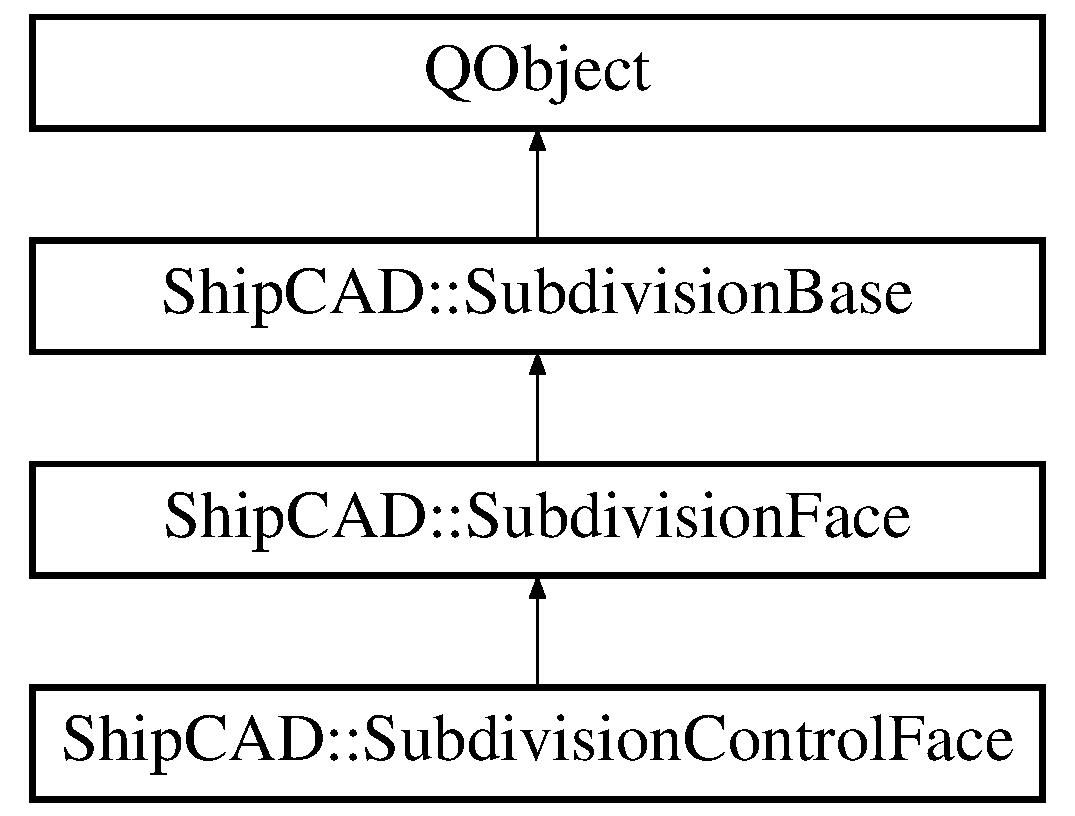
\includegraphics[height=4.000000cm]{classShipCAD_1_1SubdivisionFace}
\end{center}
\end{figure}
\subsection*{Public Member Functions}
\begin{DoxyCompactItemize}
\item 
\hyperlink{classShipCAD_1_1SubdivisionFace_a082f81f7a5750f7e53ed5a92ddc82350}{Subdivision\-Face} (\hyperlink{classShipCAD_1_1SubdivisionSurface}{Subdivision\-Surface} $\ast$owner)
\begin{DoxyCompactList}\small\item\em Constructor. \end{DoxyCompactList}\item 
virtual \hyperlink{classShipCAD_1_1SubdivisionFace_a44a0acc598533bf6846e4f7272e5c191}{$\sim$\-Subdivision\-Face} ()
\item 
void \hyperlink{classShipCAD_1_1SubdivisionFace_a16d5e005d1c7c847ccf9ba72b67142fa}{flip\-Normal} ()
\begin{DoxyCompactList}\small\item\em swap normal vector to other face \end{DoxyCompactList}\item 
void \hyperlink{classShipCAD_1_1SubdivisionFace_a553df49a1137f89d2df2846ffca74842}{add\-Point} (\hyperlink{classShipCAD_1_1SubdivisionPoint}{Subdivision\-Point} $\ast$point)
\begin{DoxyCompactList}\small\item\em add a point to the face \end{DoxyCompactList}\item 
void \hyperlink{classShipCAD_1_1SubdivisionFace_aacd383eb085c4f6b92db89e25be6b3a1}{insert\-Point} (size\-\_\-t index, \hyperlink{classShipCAD_1_1SubdivisionPoint}{Subdivision\-Point} $\ast$point)
\begin{DoxyCompactList}\small\item\em insert a new point into the face \end{DoxyCompactList}\item 
virtual void \hyperlink{classShipCAD_1_1SubdivisionFace_a413ae7e76f559780c8a69e998974fb75}{clear} ()
\begin{DoxyCompactList}\small\item\em reset point attributes to default values \end{DoxyCompactList}\item 
virtual void \hyperlink{classShipCAD_1_1SubdivisionFace_a934edbf44e524a2ec250f896c3cc182d}{subdivide} (bool controlface, std\-::vector$<$ std\-::pair$<$ \hyperlink{classShipCAD_1_1SubdivisionPoint}{Subdivision\-Point} $\ast$, \hyperlink{classShipCAD_1_1SubdivisionPoint}{Subdivision\-Point} $\ast$ $>$ $>$ \&vertexpoints, std\-::vector$<$ std\-::pair$<$ \hyperlink{classShipCAD_1_1SubdivisionEdge}{Subdivision\-Edge} $\ast$, \hyperlink{classShipCAD_1_1SubdivisionPoint}{Subdivision\-Point} $\ast$ $>$ $>$ \&edgepoints, std\-::vector$<$ std\-::pair$<$ \hyperlink{classShipCAD_1_1SubdivisionFace}{Subdivision\-Face} $\ast$, \hyperlink{classShipCAD_1_1SubdivisionPoint}{Subdivision\-Point} $\ast$ $>$ $>$ \&facepoints, std\-::vector$<$ \hyperlink{classShipCAD_1_1SubdivisionEdge}{Subdivision\-Edge} $\ast$ $>$ \&interioredges, std\-::vector$<$ \hyperlink{classShipCAD_1_1SubdivisionEdge}{Subdivision\-Edge} $\ast$ $>$ \&controledges, std\-::vector$<$ \hyperlink{classShipCAD_1_1SubdivisionFace}{Subdivision\-Face} $\ast$ $>$ \&dest)
\begin{DoxyCompactList}\small\item\em subdivide the face \end{DoxyCompactList}\item 
size\-\_\-t \hyperlink{classShipCAD_1_1SubdivisionFace_ad56c693e21a77c3676430babcf49de7e}{number\-Of\-Points} ()
\begin{DoxyCompactList}\small\item\em number of points for this face \end{DoxyCompactList}\item 
bool \hyperlink{classShipCAD_1_1SubdivisionFace_a575f9199178fc28c9229fa4c7d2824ef}{has\-Point} (\hyperlink{classShipCAD_1_1SubdivisionPoint}{Subdivision\-Point} $\ast$pt)
\begin{DoxyCompactList}\small\item\em does the face have this point \end{DoxyCompactList}\item 
\hyperlink{classShipCAD_1_1SubdivisionPoint}{Subdivision\-Point} $\ast$ \hyperlink{classShipCAD_1_1SubdivisionFace_a0df579a3063c124ca2355eba4ece7480}{get\-Point} (size\-\_\-t index)
\begin{DoxyCompactList}\small\item\em get face point \end{DoxyCompactList}\item 
\hyperlink{classShipCAD_1_1SubdivisionPoint}{Subdivision\-Point} $\ast$ \hyperlink{classShipCAD_1_1SubdivisionFace_aeb9c6f01f3896dc39819265922a04892}{calculate\-Face\-Point} ()
\begin{DoxyCompactList}\small\item\em Get point on center of face for subdivision. \end{DoxyCompactList}\item 
size\-\_\-t \hyperlink{classShipCAD_1_1SubdivisionFace_a8b32525b95c836e065cb124a61caec61}{index\-Of\-Point} (\hyperlink{classShipCAD_1_1SubdivisionPoint}{Subdivision\-Point} $\ast$pt)
\begin{DoxyCompactList}\small\item\em get index of point in parent surface \end{DoxyCompactList}\item 
float \hyperlink{classShipCAD_1_1SubdivisionFace_ace99f0fe3b54e57912e5391e0aff84ea}{get\-Area} ()
\begin{DoxyCompactList}\small\item\em calculate the area of this face \end{DoxyCompactList}\item 
Q\-Vector3\-D \hyperlink{classShipCAD_1_1SubdivisionFace_a3574fd6a4241a81faa7f2ff741d07811}{get\-Face\-Center} ()
\begin{DoxyCompactList}\small\item\em get coordinates of the center of the face \end{DoxyCompactList}\item 
Q\-Vector3\-D \hyperlink{classShipCAD_1_1SubdivisionFace_add361089333f9d08a411d16ea1782246}{get\-Face\-Normal} ()
\begin{DoxyCompactList}\small\item\em get coordinates of the face normal \end{DoxyCompactList}\item 
virtual void \hyperlink{classShipCAD_1_1SubdivisionFace_aa5bd261ae5fc0a1c7fe8cc5328b8477f}{dump} (std\-::ostream \&os, const char $\ast$prefix=\char`\"{}\char`\"{}) const 
\begin{DoxyCompactList}\small\item\em print out the element to a stream \end{DoxyCompactList}\end{DoxyCompactItemize}
\subsection*{Static Public Member Functions}
\begin{DoxyCompactItemize}
\item 
static \hyperlink{classShipCAD_1_1SubdivisionFace}{Subdivision\-Face} $\ast$ \hyperlink{classShipCAD_1_1SubdivisionFace_a4a6f182fa7e5cf63fc95c7614805f136}{construct} (\hyperlink{classShipCAD_1_1SubdivisionSurface}{Subdivision\-Surface} $\ast$owner)
\end{DoxyCompactItemize}
\subsection*{Protected Member Functions}
\begin{DoxyCompactItemize}
\item 
void \hyperlink{classShipCAD_1_1SubdivisionFace_ab2f647963b552728f40d8c329318676e}{priv\-\_\-dump} (std\-::ostream \&os, const char $\ast$prefix) const 
\item 
void \hyperlink{classShipCAD_1_1SubdivisionFace_a5399f7ec8ed458f6dbc733688c006cf8}{edge\-Check} (\hyperlink{classShipCAD_1_1SubdivisionPoint}{Subdivision\-Point} $\ast$p1, \hyperlink{classShipCAD_1_1SubdivisionPoint}{Subdivision\-Point} $\ast$p2, bool crease, bool controledge, \hyperlink{classShipCAD_1_1SubdivisionControlCurve}{Subdivision\-Control\-Curve} $\ast$curve, std\-::vector$<$ \hyperlink{classShipCAD_1_1SubdivisionEdge}{Subdivision\-Edge} $\ast$ $>$ \&interioredges, std\-::vector$<$ \hyperlink{classShipCAD_1_1SubdivisionEdge}{Subdivision\-Edge} $\ast$ $>$ \&controledges)
\begin{DoxyCompactList}\small\item\em check for edge between points \end{DoxyCompactList}\end{DoxyCompactItemize}
\subsection*{Protected Attributes}
\begin{DoxyCompactItemize}
\item 
std\-::vector$<$ \hyperlink{classShipCAD_1_1SubdivisionPoint}{Subdivision\-Point} $\ast$ $>$ \hyperlink{classShipCAD_1_1SubdivisionFace_ae1178fe10860c57e3e54a397b4dc7b4b}{\-\_\-points}
\end{DoxyCompactItemize}
\subsection*{Properties}
\begin{DoxyCompactItemize}
\item 
float \hyperlink{classShipCAD_1_1SubdivisionFace_a88e0042b53b3830a523dfb782f3af6d5}{Area}
\item 
Q\-Vector3\-D \hyperlink{classShipCAD_1_1SubdivisionFace_a8daac1b66fdaee14e3f8fb443106162e}{Face\-Center}
\item 
Q\-Vector3\-D \hyperlink{classShipCAD_1_1SubdivisionFace_a44c07f86c9225ad2c463b259288fca94}{Face\-Normal}
\end{DoxyCompactItemize}


\subsection{Detailed Description}


Definition at line 56 of file subdivface.\-h.



\subsection{Constructor \& Destructor Documentation}
\hypertarget{classShipCAD_1_1SubdivisionFace_a082f81f7a5750f7e53ed5a92ddc82350}{\index{Ship\-C\-A\-D\-::\-Subdivision\-Face@{Ship\-C\-A\-D\-::\-Subdivision\-Face}!Subdivision\-Face@{Subdivision\-Face}}
\index{Subdivision\-Face@{Subdivision\-Face}!ShipCAD::SubdivisionFace@{Ship\-C\-A\-D\-::\-Subdivision\-Face}}
\subsubsection[{Subdivision\-Face}]{\setlength{\rightskip}{0pt plus 5cm}Subdivision\-Face\-::\-Subdivision\-Face (
\begin{DoxyParamCaption}
\item[{{\bf Subdivision\-Surface} $\ast$}]{owner}
\end{DoxyParamCaption}
)\hspace{0.3cm}{\ttfamily [explicit]}}}\label{classShipCAD_1_1SubdivisionFace_a082f81f7a5750f7e53ed5a92ddc82350}


Constructor. 


\begin{DoxyParams}{Parameters}
{\em owner} & parent surface \\
\hline
\end{DoxyParams}


Definition at line 60 of file subdivface.\-cpp.

\hypertarget{classShipCAD_1_1SubdivisionFace_a44a0acc598533bf6846e4f7272e5c191}{\index{Ship\-C\-A\-D\-::\-Subdivision\-Face@{Ship\-C\-A\-D\-::\-Subdivision\-Face}!$\sim$\-Subdivision\-Face@{$\sim$\-Subdivision\-Face}}
\index{$\sim$\-Subdivision\-Face@{$\sim$\-Subdivision\-Face}!ShipCAD::SubdivisionFace@{Ship\-C\-A\-D\-::\-Subdivision\-Face}}
\subsubsection[{$\sim$\-Subdivision\-Face}]{\setlength{\rightskip}{0pt plus 5cm}Subdivision\-Face\-::$\sim$\-Subdivision\-Face (
\begin{DoxyParamCaption}
{}
\end{DoxyParamCaption}
)\hspace{0.3cm}{\ttfamily [virtual]}}}\label{classShipCAD_1_1SubdivisionFace_a44a0acc598533bf6846e4f7272e5c191}


Definition at line 66 of file subdivface.\-cpp.



\subsection{Member Function Documentation}
\hypertarget{classShipCAD_1_1SubdivisionFace_a553df49a1137f89d2df2846ffca74842}{\index{Ship\-C\-A\-D\-::\-Subdivision\-Face@{Ship\-C\-A\-D\-::\-Subdivision\-Face}!add\-Point@{add\-Point}}
\index{add\-Point@{add\-Point}!ShipCAD::SubdivisionFace@{Ship\-C\-A\-D\-::\-Subdivision\-Face}}
\subsubsection[{add\-Point}]{\setlength{\rightskip}{0pt plus 5cm}void Subdivision\-Face\-::add\-Point (
\begin{DoxyParamCaption}
\item[{{\bf Subdivision\-Point} $\ast$}]{point}
\end{DoxyParamCaption}
)}}\label{classShipCAD_1_1SubdivisionFace_a553df49a1137f89d2df2846ffca74842}


add a point to the face 


\begin{DoxyParams}{Parameters}
{\em point} & point to add \\
\hline
\end{DoxyParams}


Definition at line 158 of file subdivface.\-cpp.

\hypertarget{classShipCAD_1_1SubdivisionFace_aeb9c6f01f3896dc39819265922a04892}{\index{Ship\-C\-A\-D\-::\-Subdivision\-Face@{Ship\-C\-A\-D\-::\-Subdivision\-Face}!calculate\-Face\-Point@{calculate\-Face\-Point}}
\index{calculate\-Face\-Point@{calculate\-Face\-Point}!ShipCAD::SubdivisionFace@{Ship\-C\-A\-D\-::\-Subdivision\-Face}}
\subsubsection[{calculate\-Face\-Point}]{\setlength{\rightskip}{0pt plus 5cm}{\bf Subdivision\-Point} $\ast$ Subdivision\-Face\-::calculate\-Face\-Point (
\begin{DoxyParamCaption}
{}
\end{DoxyParamCaption}
)}}\label{classShipCAD_1_1SubdivisionFace_aeb9c6f01f3896dc39819265922a04892}


Get point on center of face for subdivision. 

When subdividing a face, each edge is split, and a point is put in the center of the face, then all are connected and new faces created. If the face is a triangle and we are not using fv\-Catmull\-Clark, then a center point is not created. The face is then divided into triangles, instead of quadrilateral faces. In that case this returns a null point

\begin{DoxyReturn}{Returns}
the point at center of face, or 0 if triangle and not using fv\-Catmull\-Clark, or the number of face points is less than 3 
\end{DoxyReturn}


Definition at line 164 of file subdivface.\-cpp.

\hypertarget{classShipCAD_1_1SubdivisionFace_a413ae7e76f559780c8a69e998974fb75}{\index{Ship\-C\-A\-D\-::\-Subdivision\-Face@{Ship\-C\-A\-D\-::\-Subdivision\-Face}!clear@{clear}}
\index{clear@{clear}!ShipCAD::SubdivisionFace@{Ship\-C\-A\-D\-::\-Subdivision\-Face}}
\subsubsection[{clear}]{\setlength{\rightskip}{0pt plus 5cm}void Subdivision\-Face\-::clear (
\begin{DoxyParamCaption}
{}
\end{DoxyParamCaption}
)\hspace{0.3cm}{\ttfamily [virtual]}}}\label{classShipCAD_1_1SubdivisionFace_a413ae7e76f559780c8a69e998974fb75}


reset point attributes to default values 



Implements \hyperlink{classShipCAD_1_1SubdivisionBase_a851bb7f1931f9dd6e53b6f9df7b5b352}{Ship\-C\-A\-D\-::\-Subdivision\-Base}.



Reimplemented in \hyperlink{classShipCAD_1_1SubdivisionControlFace_ad168e31f0ef2537b3cd0f58b0c1c54e2}{Ship\-C\-A\-D\-::\-Subdivision\-Control\-Face}.



Definition at line 182 of file subdivface.\-cpp.

\hypertarget{classShipCAD_1_1SubdivisionFace_a4a6f182fa7e5cf63fc95c7614805f136}{\index{Ship\-C\-A\-D\-::\-Subdivision\-Face@{Ship\-C\-A\-D\-::\-Subdivision\-Face}!construct@{construct}}
\index{construct@{construct}!ShipCAD::SubdivisionFace@{Ship\-C\-A\-D\-::\-Subdivision\-Face}}
\subsubsection[{construct}]{\setlength{\rightskip}{0pt plus 5cm}{\bf Subdivision\-Face} $\ast$ Subdivision\-Face\-::construct (
\begin{DoxyParamCaption}
\item[{{\bf Subdivision\-Surface} $\ast$}]{owner}
\end{DoxyParamCaption}
)\hspace{0.3cm}{\ttfamily [static]}}}\label{classShipCAD_1_1SubdivisionFace_a4a6f182fa7e5cf63fc95c7614805f136}


Definition at line 52 of file subdivface.\-cpp.

\hypertarget{classShipCAD_1_1SubdivisionFace_aa5bd261ae5fc0a1c7fe8cc5328b8477f}{\index{Ship\-C\-A\-D\-::\-Subdivision\-Face@{Ship\-C\-A\-D\-::\-Subdivision\-Face}!dump@{dump}}
\index{dump@{dump}!ShipCAD::SubdivisionFace@{Ship\-C\-A\-D\-::\-Subdivision\-Face}}
\subsubsection[{dump}]{\setlength{\rightskip}{0pt plus 5cm}void Subdivision\-Face\-::dump (
\begin{DoxyParamCaption}
\item[{std\-::ostream \&}]{os, }
\item[{const char $\ast$}]{prefix = {\ttfamily \char`\"{}\char`\"{}}}
\end{DoxyParamCaption}
) const\hspace{0.3cm}{\ttfamily [virtual]}}}\label{classShipCAD_1_1SubdivisionFace_aa5bd261ae5fc0a1c7fe8cc5328b8477f}


print out the element to a stream 


\begin{DoxyParams}{Parameters}
{\em os} & the output stream \\
\hline
{\em prefix} & string to prefix on each line output \\
\hline
\end{DoxyParams}


Reimplemented from \hyperlink{classShipCAD_1_1SubdivisionBase_a7807e64ac8d2acc3da572e03cf0523b6}{Ship\-C\-A\-D\-::\-Subdivision\-Base}.



Reimplemented in \hyperlink{classShipCAD_1_1SubdivisionControlFace_a947868fba3e9bb6c587847fb9245c9ff}{Ship\-C\-A\-D\-::\-Subdivision\-Control\-Face}.



Definition at line 386 of file subdivface.\-cpp.

\hypertarget{classShipCAD_1_1SubdivisionFace_a5399f7ec8ed458f6dbc733688c006cf8}{\index{Ship\-C\-A\-D\-::\-Subdivision\-Face@{Ship\-C\-A\-D\-::\-Subdivision\-Face}!edge\-Check@{edge\-Check}}
\index{edge\-Check@{edge\-Check}!ShipCAD::SubdivisionFace@{Ship\-C\-A\-D\-::\-Subdivision\-Face}}
\subsubsection[{edge\-Check}]{\setlength{\rightskip}{0pt plus 5cm}void Subdivision\-Face\-::edge\-Check (
\begin{DoxyParamCaption}
\item[{{\bf Subdivision\-Point} $\ast$}]{p1, }
\item[{{\bf Subdivision\-Point} $\ast$}]{p2, }
\item[{bool}]{crease, }
\item[{bool}]{controledge, }
\item[{{\bf Subdivision\-Control\-Curve} $\ast$}]{curve, }
\item[{std\-::vector$<$ {\bf Subdivision\-Edge} $\ast$ $>$ \&}]{interioredges, }
\item[{std\-::vector$<$ {\bf Subdivision\-Edge} $\ast$ $>$ \&}]{controledges}
\end{DoxyParamCaption}
)\hspace{0.3cm}{\ttfamily [protected]}}}\label{classShipCAD_1_1SubdivisionFace_a5399f7ec8ed458f6dbc733688c006cf8}


check for edge between points 

This method will create edges between 2 points if it doesn't exist.


\begin{DoxyParams}{Parameters}
{\em p1} & start point of edge \\
\hline
{\em p2} & end point of edge \\
\hline
{\em crease} & whether this edge is a crease \\
\hline
{\em controledge} & whether this edge is a control edge \\
\hline
{\em curve} & if edge is a controledge, then pass the curve to be attached \\
\hline
{\em interioredges} & if this edge is an interior edge, add it to this list \\
\hline
{\em controledges} & if this edge is a control, add it to this list \\
\hline
\end{DoxyParams}


Definition at line 196 of file subdivface.\-cpp.

\hypertarget{classShipCAD_1_1SubdivisionFace_a16d5e005d1c7c847ccf9ba72b67142fa}{\index{Ship\-C\-A\-D\-::\-Subdivision\-Face@{Ship\-C\-A\-D\-::\-Subdivision\-Face}!flip\-Normal@{flip\-Normal}}
\index{flip\-Normal@{flip\-Normal}!ShipCAD::SubdivisionFace@{Ship\-C\-A\-D\-::\-Subdivision\-Face}}
\subsubsection[{flip\-Normal}]{\setlength{\rightskip}{0pt plus 5cm}void Subdivision\-Face\-::flip\-Normal (
\begin{DoxyParamCaption}
{}
\end{DoxyParamCaption}
)}}\label{classShipCAD_1_1SubdivisionFace_a16d5e005d1c7c847ccf9ba72b67142fa}


swap normal vector to other face 



Definition at line 187 of file subdivface.\-cpp.

\hypertarget{classShipCAD_1_1SubdivisionFace_ace99f0fe3b54e57912e5391e0aff84ea}{\index{Ship\-C\-A\-D\-::\-Subdivision\-Face@{Ship\-C\-A\-D\-::\-Subdivision\-Face}!get\-Area@{get\-Area}}
\index{get\-Area@{get\-Area}!ShipCAD::SubdivisionFace@{Ship\-C\-A\-D\-::\-Subdivision\-Face}}
\subsubsection[{get\-Area}]{\setlength{\rightskip}{0pt plus 5cm}float Subdivision\-Face\-::get\-Area (
\begin{DoxyParamCaption}
{}
\end{DoxyParamCaption}
)}}\label{classShipCAD_1_1SubdivisionFace_ace99f0fe3b54e57912e5391e0aff84ea}


calculate the area of this face 



Definition at line 97 of file subdivface.\-cpp.

\hypertarget{classShipCAD_1_1SubdivisionFace_a3574fd6a4241a81faa7f2ff741d07811}{\index{Ship\-C\-A\-D\-::\-Subdivision\-Face@{Ship\-C\-A\-D\-::\-Subdivision\-Face}!get\-Face\-Center@{get\-Face\-Center}}
\index{get\-Face\-Center@{get\-Face\-Center}!ShipCAD::SubdivisionFace@{Ship\-C\-A\-D\-::\-Subdivision\-Face}}
\subsubsection[{get\-Face\-Center}]{\setlength{\rightskip}{0pt plus 5cm}Q\-Vector3\-D Subdivision\-Face\-::get\-Face\-Center (
\begin{DoxyParamCaption}
{}
\end{DoxyParamCaption}
)}}\label{classShipCAD_1_1SubdivisionFace_a3574fd6a4241a81faa7f2ff741d07811}


get coordinates of the center of the face 

\begin{DoxyReturn}{Returns}
coordinates of the face center 
\end{DoxyReturn}


Definition at line 107 of file subdivface.\-cpp.

\hypertarget{classShipCAD_1_1SubdivisionFace_add361089333f9d08a411d16ea1782246}{\index{Ship\-C\-A\-D\-::\-Subdivision\-Face@{Ship\-C\-A\-D\-::\-Subdivision\-Face}!get\-Face\-Normal@{get\-Face\-Normal}}
\index{get\-Face\-Normal@{get\-Face\-Normal}!ShipCAD::SubdivisionFace@{Ship\-C\-A\-D\-::\-Subdivision\-Face}}
\subsubsection[{get\-Face\-Normal}]{\setlength{\rightskip}{0pt plus 5cm}Q\-Vector3\-D Subdivision\-Face\-::get\-Face\-Normal (
\begin{DoxyParamCaption}
{}
\end{DoxyParamCaption}
)}}\label{classShipCAD_1_1SubdivisionFace_add361089333f9d08a411d16ea1782246}


get coordinates of the face normal 

\begin{DoxyReturn}{Returns}
coordinates of the face normal 
\end{DoxyReturn}


Definition at line 120 of file subdivface.\-cpp.

\hypertarget{classShipCAD_1_1SubdivisionFace_a0df579a3063c124ca2355eba4ece7480}{\index{Ship\-C\-A\-D\-::\-Subdivision\-Face@{Ship\-C\-A\-D\-::\-Subdivision\-Face}!get\-Point@{get\-Point}}
\index{get\-Point@{get\-Point}!ShipCAD::SubdivisionFace@{Ship\-C\-A\-D\-::\-Subdivision\-Face}}
\subsubsection[{get\-Point}]{\setlength{\rightskip}{0pt plus 5cm}{\bf Subdivision\-Point} $\ast$ Subdivision\-Face\-::get\-Point (
\begin{DoxyParamCaption}
\item[{size\-\_\-t}]{index}
\end{DoxyParamCaption}
)}}\label{classShipCAD_1_1SubdivisionFace_a0df579a3063c124ca2355eba4ece7480}


get face point 


\begin{DoxyParams}{Parameters}
{\em index} & index of point to get \\
\hline
\end{DoxyParams}
\begin{DoxyReturn}{Returns}
the point at index 
\end{DoxyReturn}


Definition at line 151 of file subdivface.\-cpp.

\hypertarget{classShipCAD_1_1SubdivisionFace_a575f9199178fc28c9229fa4c7d2824ef}{\index{Ship\-C\-A\-D\-::\-Subdivision\-Face@{Ship\-C\-A\-D\-::\-Subdivision\-Face}!has\-Point@{has\-Point}}
\index{has\-Point@{has\-Point}!ShipCAD::SubdivisionFace@{Ship\-C\-A\-D\-::\-Subdivision\-Face}}
\subsubsection[{has\-Point}]{\setlength{\rightskip}{0pt plus 5cm}bool Subdivision\-Face\-::has\-Point (
\begin{DoxyParamCaption}
\item[{{\bf Subdivision\-Point} $\ast$}]{pt}
\end{DoxyParamCaption}
)}}\label{classShipCAD_1_1SubdivisionFace_a575f9199178fc28c9229fa4c7d2824ef}


does the face have this point 


\begin{DoxyParams}{Parameters}
{\em pt} & the point to check \\
\hline
\end{DoxyParams}
\begin{DoxyReturn}{Returns}
true if the point is part of the face 
\end{DoxyReturn}


Definition at line 146 of file subdivface.\-cpp.

\hypertarget{classShipCAD_1_1SubdivisionFace_a8b32525b95c836e065cb124a61caec61}{\index{Ship\-C\-A\-D\-::\-Subdivision\-Face@{Ship\-C\-A\-D\-::\-Subdivision\-Face}!index\-Of\-Point@{index\-Of\-Point}}
\index{index\-Of\-Point@{index\-Of\-Point}!ShipCAD::SubdivisionFace@{Ship\-C\-A\-D\-::\-Subdivision\-Face}}
\subsubsection[{index\-Of\-Point}]{\setlength{\rightskip}{0pt plus 5cm}size\-\_\-t Subdivision\-Face\-::index\-Of\-Point (
\begin{DoxyParamCaption}
\item[{{\bf Subdivision\-Point} $\ast$}]{pt}
\end{DoxyParamCaption}
)}}\label{classShipCAD_1_1SubdivisionFace_a8b32525b95c836e065cb124a61caec61}


get index of point in parent surface 


\begin{DoxyParams}{Parameters}
{\em pt} & point to find in parent surface \\
\hline
\end{DoxyParams}
\begin{DoxyReturn}{Returns}
index of that point in parent surface 
\end{DoxyReturn}


Definition at line 71 of file subdivface.\-cpp.

\hypertarget{classShipCAD_1_1SubdivisionFace_aacd383eb085c4f6b92db89e25be6b3a1}{\index{Ship\-C\-A\-D\-::\-Subdivision\-Face@{Ship\-C\-A\-D\-::\-Subdivision\-Face}!insert\-Point@{insert\-Point}}
\index{insert\-Point@{insert\-Point}!ShipCAD::SubdivisionFace@{Ship\-C\-A\-D\-::\-Subdivision\-Face}}
\subsubsection[{insert\-Point}]{\setlength{\rightskip}{0pt plus 5cm}void Subdivision\-Face\-::insert\-Point (
\begin{DoxyParamCaption}
\item[{size\-\_\-t}]{index, }
\item[{{\bf Subdivision\-Point} $\ast$}]{point}
\end{DoxyParamCaption}
)}}\label{classShipCAD_1_1SubdivisionFace_aacd383eb085c4f6b92db89e25be6b3a1}


insert a new point into the face 


\begin{DoxyParams}{Parameters}
{\em index} & insert the new point at this index \\
\hline
{\em point} & point to add to face \\
\hline
\end{DoxyParams}


Definition at line 76 of file subdivface.\-cpp.

\hypertarget{classShipCAD_1_1SubdivisionFace_ad56c693e21a77c3676430babcf49de7e}{\index{Ship\-C\-A\-D\-::\-Subdivision\-Face@{Ship\-C\-A\-D\-::\-Subdivision\-Face}!number\-Of\-Points@{number\-Of\-Points}}
\index{number\-Of\-Points@{number\-Of\-Points}!ShipCAD::SubdivisionFace@{Ship\-C\-A\-D\-::\-Subdivision\-Face}}
\subsubsection[{number\-Of\-Points}]{\setlength{\rightskip}{0pt plus 5cm}size\-\_\-t Ship\-C\-A\-D\-::\-Subdivision\-Face\-::number\-Of\-Points (
\begin{DoxyParamCaption}
{}
\end{DoxyParamCaption}
)\hspace{0.3cm}{\ttfamily [inline]}}}\label{classShipCAD_1_1SubdivisionFace_ad56c693e21a77c3676430babcf49de7e}


number of points for this face 

\begin{DoxyReturn}{Returns}
number of points for this face 
\end{DoxyReturn}


Definition at line 125 of file subdivface.\-h.

\hypertarget{classShipCAD_1_1SubdivisionFace_ab2f647963b552728f40d8c329318676e}{\index{Ship\-C\-A\-D\-::\-Subdivision\-Face@{Ship\-C\-A\-D\-::\-Subdivision\-Face}!priv\-\_\-dump@{priv\-\_\-dump}}
\index{priv\-\_\-dump@{priv\-\_\-dump}!ShipCAD::SubdivisionFace@{Ship\-C\-A\-D\-::\-Subdivision\-Face}}
\subsubsection[{priv\-\_\-dump}]{\setlength{\rightskip}{0pt plus 5cm}void Subdivision\-Face\-::priv\-\_\-dump (
\begin{DoxyParamCaption}
\item[{std\-::ostream \&}]{os, }
\item[{const char $\ast$}]{prefix}
\end{DoxyParamCaption}
) const\hspace{0.3cm}{\ttfamily [protected]}}}\label{classShipCAD_1_1SubdivisionFace_ab2f647963b552728f40d8c329318676e}


Definition at line 393 of file subdivface.\-cpp.

\hypertarget{classShipCAD_1_1SubdivisionFace_a934edbf44e524a2ec250f896c3cc182d}{\index{Ship\-C\-A\-D\-::\-Subdivision\-Face@{Ship\-C\-A\-D\-::\-Subdivision\-Face}!subdivide@{subdivide}}
\index{subdivide@{subdivide}!ShipCAD::SubdivisionFace@{Ship\-C\-A\-D\-::\-Subdivision\-Face}}
\subsubsection[{subdivide}]{\setlength{\rightskip}{0pt plus 5cm}void Subdivision\-Face\-::subdivide (
\begin{DoxyParamCaption}
\item[{bool}]{controlface, }
\item[{std\-::vector$<$ std\-::pair$<$ {\bf Subdivision\-Point} $\ast$, {\bf Subdivision\-Point} $\ast$ $>$ $>$ \&}]{vertexpoints, }
\item[{std\-::vector$<$ std\-::pair$<$ {\bf Subdivision\-Edge} $\ast$, {\bf Subdivision\-Point} $\ast$ $>$ $>$ \&}]{edgepoints, }
\item[{std\-::vector$<$ std\-::pair$<$ {\bf Subdivision\-Face} $\ast$, {\bf Subdivision\-Point} $\ast$ $>$ $>$ \&}]{facepoints, }
\item[{std\-::vector$<$ {\bf Subdivision\-Edge} $\ast$ $>$ \&}]{interioredges, }
\item[{std\-::vector$<$ {\bf Subdivision\-Edge} $\ast$ $>$ \&}]{controledges, }
\item[{std\-::vector$<$ {\bf Subdivision\-Face} $\ast$ $>$ \&}]{dest}
\end{DoxyParamCaption}
)\hspace{0.3cm}{\ttfamily [virtual]}}}\label{classShipCAD_1_1SubdivisionFace_a934edbf44e524a2ec250f896c3cc182d}


subdivide the face 


\begin{DoxyParams}{Parameters}
{\em vertexpoints} & list of Point $<$-\/$>$ Point pairs. The first point is a vertex point on this face, the second point is a copy of this point to use in the new subdivided faces\\
\hline
{\em edgepoints} & list of Edge $<$-\/$>$ Point pairs. The edge is an edge on this face. The point is the midpoint of that edge to use in the new subdivided faces\\
\hline
{\em facepoints} & list of Face $<$-\/$>$ Point pairs.\\
\hline
{\em interioredges} & after subdivision, the new interior edges of the newly created faces will be added to this list\\
\hline
{\em controledges} & after subdivision, the new edges descended from control edges will be added to this list\\
\hline
{\em dest} & the new subdivided faces will be added to this list \\
\hline
\end{DoxyParams}


Definition at line 261 of file subdivface.\-cpp.



\subsection{Member Data Documentation}
\hypertarget{classShipCAD_1_1SubdivisionFace_ae1178fe10860c57e3e54a397b4dc7b4b}{\index{Ship\-C\-A\-D\-::\-Subdivision\-Face@{Ship\-C\-A\-D\-::\-Subdivision\-Face}!\-\_\-points@{\-\_\-points}}
\index{\-\_\-points@{\-\_\-points}!ShipCAD::SubdivisionFace@{Ship\-C\-A\-D\-::\-Subdivision\-Face}}
\subsubsection[{\-\_\-points}]{\setlength{\rightskip}{0pt plus 5cm}std\-::vector$<${\bf Subdivision\-Point}$\ast$$>$ Ship\-C\-A\-D\-::\-Subdivision\-Face\-::\-\_\-points\hspace{0.3cm}{\ttfamily [protected]}}}\label{classShipCAD_1_1SubdivisionFace_ae1178fe10860c57e3e54a397b4dc7b4b}
points belonging to this face 

Definition at line 203 of file subdivface.\-h.



\subsection{Property Documentation}
\hypertarget{classShipCAD_1_1SubdivisionFace_a88e0042b53b3830a523dfb782f3af6d5}{\index{Ship\-C\-A\-D\-::\-Subdivision\-Face@{Ship\-C\-A\-D\-::\-Subdivision\-Face}!Area@{Area}}
\index{Area@{Area}!ShipCAD::SubdivisionFace@{Ship\-C\-A\-D\-::\-Subdivision\-Face}}
\subsubsection[{Area}]{\setlength{\rightskip}{0pt plus 5cm}float Ship\-C\-A\-D\-::\-Subdivision\-Face\-::\-Area\hspace{0.3cm}{\ttfamily [read]}}}\label{classShipCAD_1_1SubdivisionFace_a88e0042b53b3830a523dfb782f3af6d5}


Definition at line 59 of file subdivface.\-h.

\hypertarget{classShipCAD_1_1SubdivisionFace_a8daac1b66fdaee14e3f8fb443106162e}{\index{Ship\-C\-A\-D\-::\-Subdivision\-Face@{Ship\-C\-A\-D\-::\-Subdivision\-Face}!Face\-Center@{Face\-Center}}
\index{Face\-Center@{Face\-Center}!ShipCAD::SubdivisionFace@{Ship\-C\-A\-D\-::\-Subdivision\-Face}}
\subsubsection[{Face\-Center}]{\setlength{\rightskip}{0pt plus 5cm}Q\-Vector3\-D Ship\-C\-A\-D\-::\-Subdivision\-Face\-::\-Face\-Center\hspace{0.3cm}{\ttfamily [read]}}}\label{classShipCAD_1_1SubdivisionFace_a8daac1b66fdaee14e3f8fb443106162e}


Definition at line 60 of file subdivface.\-h.

\hypertarget{classShipCAD_1_1SubdivisionFace_a44c07f86c9225ad2c463b259288fca94}{\index{Ship\-C\-A\-D\-::\-Subdivision\-Face@{Ship\-C\-A\-D\-::\-Subdivision\-Face}!Face\-Normal@{Face\-Normal}}
\index{Face\-Normal@{Face\-Normal}!ShipCAD::SubdivisionFace@{Ship\-C\-A\-D\-::\-Subdivision\-Face}}
\subsubsection[{Face\-Normal}]{\setlength{\rightskip}{0pt plus 5cm}Q\-Vector3\-D Ship\-C\-A\-D\-::\-Subdivision\-Face\-::\-Face\-Normal\hspace{0.3cm}{\ttfamily [read]}}}\label{classShipCAD_1_1SubdivisionFace_a44c07f86c9225ad2c463b259288fca94}


Definition at line 61 of file subdivface.\-h.



The documentation for this class was generated from the following files\-:\begin{DoxyCompactItemize}
\item 
Ship\-C\-A\-Dlib/\hyperlink{subdivface_8h}{subdivface.\-h}\item 
Ship\-C\-A\-Dlib/\hyperlink{subdivface_8cpp}{subdivface.\-cpp}\end{DoxyCompactItemize}

\hypertarget{classShipCAD_1_1SubdivisionLayer}{\section{Ship\-C\-A\-D\-:\-:Subdivision\-Layer Class Reference}
\label{classShipCAD_1_1SubdivisionLayer}\index{Ship\-C\-A\-D\-::\-Subdivision\-Layer@{Ship\-C\-A\-D\-::\-Subdivision\-Layer}}
}


{\ttfamily \#include $<$subdivlayer.\-h$>$}

Inheritance diagram for Ship\-C\-A\-D\-:\-:Subdivision\-Layer\-:\begin{figure}[H]
\begin{center}
\leavevmode
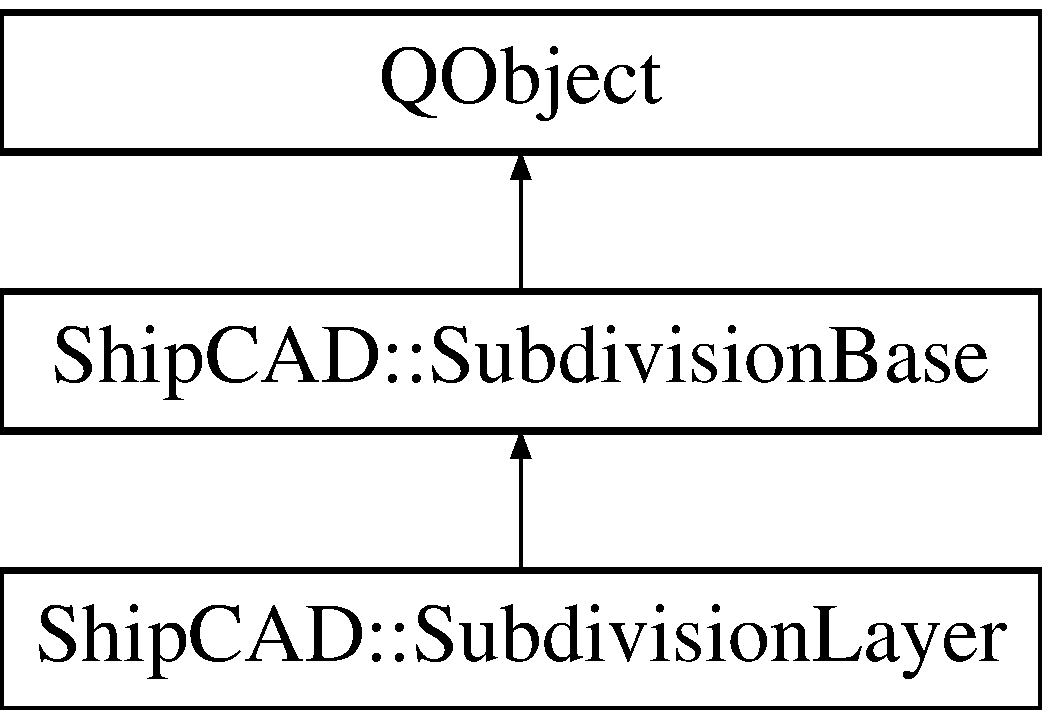
\includegraphics[height=3.000000cm]{classShipCAD_1_1SubdivisionLayer}
\end{center}
\end{figure}
\subsection*{Signals}
\begin{DoxyCompactItemize}
\item 
void \hyperlink{classShipCAD_1_1SubdivisionLayer_ad36ec152981983b8a4dc87df39071418}{changed\-Layer\-Data} (size\-\_\-t layerid)
\end{DoxyCompactItemize}
\subsection*{Public Member Functions}
\begin{DoxyCompactItemize}
\item 
\hyperlink{classShipCAD_1_1SubdivisionLayer_a788864a40265b764b8d97d9a9cbbbd13}{Subdivision\-Layer} (\hyperlink{classShipCAD_1_1SubdivisionSurface}{Subdivision\-Surface} $\ast$owner)
\item 
virtual \hyperlink{classShipCAD_1_1SubdivisionLayer_a4e852a07f46e57f28ffedd4a68c2f4c4}{$\sim$\-Subdivision\-Layer} ()
\item 
void \hyperlink{classShipCAD_1_1SubdivisionLayer_a45b3af65b8b11dd2bf566a454bc125bd}{delete\-Control\-Face} (\hyperlink{classShipCAD_1_1SubdivisionControlFace}{Subdivision\-Control\-Face} $\ast$face)
\item 
void \hyperlink{classShipCAD_1_1SubdivisionLayer_a3c966ebc7e2c1f516f2329324d5658e2}{add\-Control\-Face} (\hyperlink{classShipCAD_1_1SubdivisionControlFace}{Subdivision\-Control\-Face} $\ast$newface)
\item 
size\-\_\-t \hyperlink{classShipCAD_1_1SubdivisionLayer_a75dcc3a9944f799c72d1a87b93d92d89}{number\-Of\-Faces} ()
\item 
\hyperlink{classShipCAD_1_1SubdivisionControlFace}{Subdivision\-Control\-Face} $\ast$ \hyperlink{classShipCAD_1_1SubdivisionLayer_a2e1538a000268fe5f56bf2bea4973c23}{get\-Face} (size\-\_\-t index)
\item 
bool \hyperlink{classShipCAD_1_1SubdivisionLayer_ab2d11ebf60ad6edd818eb0c42971946c}{calculate\-Intersection\-Points} (\hyperlink{classShipCAD_1_1SubdivisionLayer}{Subdivision\-Layer} $\ast$layer)
\item 
virtual void \hyperlink{classShipCAD_1_1SubdivisionLayer_a7046d17ba87dd5ce7399f22ae327fc6e}{clear} ()
\begin{DoxyCompactList}\small\item\em reset this element to default values \end{DoxyCompactList}\item 
void \hyperlink{classShipCAD_1_1SubdivisionLayer_a319ae070f596e92307671cda0a607887}{assign\-Properties} (\hyperlink{classShipCAD_1_1SubdivisionLayer}{Subdivision\-Layer} $\ast$source)
\item 
void \hyperlink{classShipCAD_1_1SubdivisionLayer_a949c536d7c238f8ba3a33abdde8bfaa3}{move\-Down} ()
\item 
void \hyperlink{classShipCAD_1_1SubdivisionLayer_aef4dff844415352660f8cf90120b240c}{move\-Up} ()
\item 
void \hyperlink{classShipCAD_1_1SubdivisionLayer_a2fc3ac326021a97479b821331e295640}{extents} (Q\-Vector3\-D \&min, Q\-Vector3\-D \&max)
\item 
\hyperlink{structShipCAD_1_1LayerProperties}{Layer\-Properties} \hyperlink{classShipCAD_1_1SubdivisionLayer_a7d42f81a94b46f0d999a4fa7a48d57d6}{get\-Surface\-Properties} ()
\item 
bool \hyperlink{classShipCAD_1_1SubdivisionLayer_afa4ea10cf2e982c9d8dc179feb15a400}{is\-Visible} ()
\item 
bool \hyperlink{classShipCAD_1_1SubdivisionLayer_a4cc4c42849feacc4a7af21ce90e2541b}{is\-Symmetric} ()
\item 
bool \hyperlink{classShipCAD_1_1SubdivisionLayer_ad1907e05d0f60e9d7f401231198217d2}{is\-Developable} ()
\item 
bool \hyperlink{classShipCAD_1_1SubdivisionLayer_a817b83f4da64e030609d77c4984d7fb1}{use\-For\-Intersections} ()
\item 
bool \hyperlink{classShipCAD_1_1SubdivisionLayer_ab80cd9444086290d1298b9b2459a9e7b}{use\-In\-Hydrostatics} ()
\item 
bool \hyperlink{classShipCAD_1_1SubdivisionLayer_a049e7c5ca442f4b02cdad9935d999e1b}{show\-In\-Linesplan} ()
\item 
size\-\_\-t \hyperlink{classShipCAD_1_1SubdivisionLayer_a29642f60a1b67df1a42c16a6bf3b97e9}{get\-Layer\-I\-D} ()
\item 
void \hyperlink{classShipCAD_1_1SubdivisionLayer_ad6cbb87ecaadd6c31635fb86fe1a4b13}{set\-Layer\-I\-D} (size\-\_\-t newid)
\item 
size\-\_\-t \hyperlink{classShipCAD_1_1SubdivisionLayer_a9a760dcc67779d111d5e05585e939138}{get\-Layer\-Index} ()
\item 
float \hyperlink{classShipCAD_1_1SubdivisionLayer_af65aafc08837eb47eefad5fbbd562d32}{get\-Material\-Density} ()
\item 
float \hyperlink{classShipCAD_1_1SubdivisionLayer_a4d26f33298b7d44d41f3e3ee87a2d981}{get\-Thickness} ()
\item 
Q\-String \hyperlink{classShipCAD_1_1SubdivisionLayer_affb4df074a7f116ce60f51ad7b7ba230}{get\-Name} ()
\item 
Q\-String \hyperlink{classShipCAD_1_1SubdivisionLayer_acb442d69e4dcf6e09b5019b6416d2d58}{get\-Description} ()
\item 
Q\-String \hyperlink{classShipCAD_1_1SubdivisionLayer_a46633012876a7e13fac9ed9d7f262136}{get\-D\-X\-F\-Layername} ()
\item 
Q\-Color \hyperlink{classShipCAD_1_1SubdivisionLayer_a0a4de50721580a29c716e11196239578}{get\-Color} ()
\item 
float \hyperlink{classShipCAD_1_1SubdivisionLayer_a892f5e7c6638537e1a30630fc1a791a2}{get\-Alpha\-Blend} ()
\item 
void \hyperlink{classShipCAD_1_1SubdivisionLayer_a6fdfc0d208904d821349eb7380a52411}{set\-Developable} (bool val)
\item 
void \hyperlink{classShipCAD_1_1SubdivisionLayer_a6ef8702f5488a9c3c3763e8472c9a568}{set\-Description} (const Q\-String \&val)
\item 
void \hyperlink{classShipCAD_1_1SubdivisionLayer_a3861c77aeb283fbea6efe943ced83f41}{set\-Name} (const Q\-String \&val)
\item 
void \hyperlink{classShipCAD_1_1SubdivisionLayer_ab3c7c5072ba6cd411404651e8e0dca2f}{set\-Symmetric} (bool val)
\item 
void \hyperlink{classShipCAD_1_1SubdivisionLayer_a5494031433242c810e6e307bfef33e6d}{set\-Color} (Q\-Color col)
\item 
void \hyperlink{classShipCAD_1_1SubdivisionLayer_ae96292d06a3578f9c7bfbbdec342068a}{set\-Material\-Density} (float val)
\item 
void \hyperlink{classShipCAD_1_1SubdivisionLayer_ac4068bcc8287698ee23e27246de9212b}{set\-Thickness} (float val)
\item 
void \hyperlink{classShipCAD_1_1SubdivisionLayer_aa58323da0043db61eaa87672755e96d2}{set\-Show\-In\-Linesplan} (bool val)
\item 
void \hyperlink{classShipCAD_1_1SubdivisionLayer_a88897eeb2b600169ca110fc4ec4aef08}{set\-Use\-In\-Hydrostatics} (bool val)
\item 
void \hyperlink{classShipCAD_1_1SubdivisionLayer_aef63325b0ef8b700b96a7cd97c501936}{set\-Use\-For\-Intersections} (bool val)
\item 
void \hyperlink{classShipCAD_1_1SubdivisionLayer_a979723de5c5cf0f4ecea8a5f9d0968d7}{set\-Visible} (bool val)
\item 
void \hyperlink{classShipCAD_1_1SubdivisionLayer_a060357b84c0549fa7310e45680fed9bd}{load\-Binary} (\hyperlink{classShipCAD_1_1FileBuffer}{File\-Buffer} \&source)
\item 
void \hyperlink{classShipCAD_1_1SubdivisionLayer_a35b72f27a1d354dcc6f3b844687d91e8}{save\-Binary} (\hyperlink{classShipCAD_1_1FileBuffer}{File\-Buffer} \&destination)
\item 
void \hyperlink{classShipCAD_1_1SubdivisionLayer_aafdd381a2cf13c0f37072b6c3f008b05}{save\-To\-D\-X\-F} (std\-::vector$<$ Q\-String $>$ \&strings)
\item 
void \hyperlink{classShipCAD_1_1SubdivisionLayer_af86299eea0a5a472d1edfae2706e335a}{load\-From\-Stream} (size\-\_\-t \&lineno, std\-::vector$<$ Q\-String $>$ \&strings)
\item 
void \hyperlink{classShipCAD_1_1SubdivisionLayer_a502c7889a73015d4295fb922c92c78be}{save\-To\-Stream} (std\-::vector$<$ Q\-String $>$ \&strings)
\item 
virtual void \hyperlink{classShipCAD_1_1SubdivisionLayer_a86f8600ffbf3973bc31c99bdb9e5b18d}{draw} (\hyperlink{classShipCAD_1_1Viewport}{Viewport} \&vp)
\item 
virtual void \hyperlink{classShipCAD_1_1SubdivisionLayer_ab41e005f720a2bba4b2efa74bfd5943e}{dump} (std\-::ostream \&os, const char $\ast$prefix=\char`\"{}\char`\"{}) const 
\begin{DoxyCompactList}\small\item\em print out the element to a stream \end{DoxyCompactList}\end{DoxyCompactItemize}
\subsection*{Static Public Member Functions}
\begin{DoxyCompactItemize}
\item 
static void \hyperlink{classShipCAD_1_1SubdivisionLayer_a838537201ca31bc92a38585c87eb56e9}{draw\-Layers} (\hyperlink{classShipCAD_1_1Viewport}{Viewport} \&vp, \hyperlink{classShipCAD_1_1SubdivisionSurface}{Subdivision\-Surface} $\ast$surface)
\item 
static \hyperlink{classShipCAD_1_1SubdivisionLayer}{Subdivision\-Layer} $\ast$ \hyperlink{classShipCAD_1_1SubdivisionLayer_a7d41b9d0ff65032014ec52ff846f32a7}{construct} (\hyperlink{classShipCAD_1_1SubdivisionSurface}{Subdivision\-Surface} $\ast$owner)
\end{DoxyCompactItemize}
\subsection*{Protected Member Functions}
\begin{DoxyCompactItemize}
\item 
void \hyperlink{classShipCAD_1_1SubdivisionLayer_a80009b02c31a01e2de9f93d5982b9a63}{priv\-\_\-dump} (std\-::ostream \&os, const char $\ast$prefix) const 
\item 
void \hyperlink{classShipCAD_1_1SubdivisionLayer_abea7581d3e0b740de8db1dfd6bc9bf69}{process\-Triangle} (const Q\-Vector3\-D \&p1, const Q\-Vector3\-D \&p2, const Q\-Vector3\-D \&p3, \hyperlink{structShipCAD_1_1LayerProperties}{Layer\-Properties} \&props)
\end{DoxyCompactItemize}
\subsection*{Protected Attributes}
\begin{DoxyCompactItemize}
\item 
size\-\_\-t \hyperlink{classShipCAD_1_1SubdivisionLayer_a73e4956d179d6ebd6c062e7e76bca196}{\-\_\-layerid}
\item 
Q\-Color \hyperlink{classShipCAD_1_1SubdivisionLayer_a6da22248952737662360fa3b2730a35f}{\-\_\-color}
\item 
bool \hyperlink{classShipCAD_1_1SubdivisionLayer_a2d606476aba40bbbfc115c449f46ac26}{\-\_\-visible}
\item 
Q\-String \hyperlink{classShipCAD_1_1SubdivisionLayer_a33bbfedf8f0d130d91c74a65a575eb2a}{\-\_\-desc}
\item 
bool \hyperlink{classShipCAD_1_1SubdivisionLayer_aaeddcdf1d08d84c76c5453f4a71fbe7a}{\-\_\-symmetric}
\item 
bool \hyperlink{classShipCAD_1_1SubdivisionLayer_a81dad738f58f9b4632c1575d0b59ddb0}{\-\_\-developable}
\item 
bool \hyperlink{classShipCAD_1_1SubdivisionLayer_a8213aa3e02493472fb11949f595446f2}{\-\_\-use\-\_\-for\-\_\-intersections}
\item 
bool \hyperlink{classShipCAD_1_1SubdivisionLayer_ad36d65882f0c46ff1b3ced7d48c173f4}{\-\_\-use\-\_\-in\-\_\-hydrostatics}
\item 
bool \hyperlink{classShipCAD_1_1SubdivisionLayer_a373fd987b5f973a995517e7f97fda5ac}{\-\_\-show\-\_\-in\-\_\-linesplan}
\item 
float \hyperlink{classShipCAD_1_1SubdivisionLayer_adfdd4e996a5be7147a2eeb682dd93ff8}{\-\_\-material\-\_\-density}
\item 
float \hyperlink{classShipCAD_1_1SubdivisionLayer_a00a308fdf03a0c1d9a6fa65f965e7942}{\-\_\-thickness}
\item 
unsigned char \hyperlink{classShipCAD_1_1SubdivisionLayer_a1681170da038b0708d1b4dcd2ec89b81}{\-\_\-alphablend}
\item 
std\-::vector\\*
$<$ \hyperlink{classShipCAD_1_1SubdivisionControlFace}{Subdivision\-Control\-Face} $\ast$ $>$ \hyperlink{classShipCAD_1_1SubdivisionLayer_a98b25b86a7104e4f987d34506438113f}{\-\_\-patches}
\end{DoxyCompactItemize}
\subsection*{Additional Inherited Members}


\subsection{Detailed Description}


Definition at line 65 of file subdivlayer.\-h.



\subsection{Constructor \& Destructor Documentation}
\hypertarget{classShipCAD_1_1SubdivisionLayer_a788864a40265b764b8d97d9a9cbbbd13}{\index{Ship\-C\-A\-D\-::\-Subdivision\-Layer@{Ship\-C\-A\-D\-::\-Subdivision\-Layer}!Subdivision\-Layer@{Subdivision\-Layer}}
\index{Subdivision\-Layer@{Subdivision\-Layer}!ShipCAD::SubdivisionLayer@{Ship\-C\-A\-D\-::\-Subdivision\-Layer}}
\subsubsection[{Subdivision\-Layer}]{\setlength{\rightskip}{0pt plus 5cm}Subdivision\-Layer\-::\-Subdivision\-Layer (
\begin{DoxyParamCaption}
\item[{{\bf Subdivision\-Surface} $\ast$}]{owner}
\end{DoxyParamCaption}
)\hspace{0.3cm}{\ttfamily [explicit]}}}\label{classShipCAD_1_1SubdivisionLayer_a788864a40265b764b8d97d9a9cbbbd13}


Definition at line 56 of file subdivlayer.\-cpp.

\hypertarget{classShipCAD_1_1SubdivisionLayer_a4e852a07f46e57f28ffedd4a68c2f4c4}{\index{Ship\-C\-A\-D\-::\-Subdivision\-Layer@{Ship\-C\-A\-D\-::\-Subdivision\-Layer}!$\sim$\-Subdivision\-Layer@{$\sim$\-Subdivision\-Layer}}
\index{$\sim$\-Subdivision\-Layer@{$\sim$\-Subdivision\-Layer}!ShipCAD::SubdivisionLayer@{Ship\-C\-A\-D\-::\-Subdivision\-Layer}}
\subsubsection[{$\sim$\-Subdivision\-Layer}]{\setlength{\rightskip}{0pt plus 5cm}Subdivision\-Layer\-::$\sim$\-Subdivision\-Layer (
\begin{DoxyParamCaption}
{}
\end{DoxyParamCaption}
)\hspace{0.3cm}{\ttfamily [virtual]}}}\label{classShipCAD_1_1SubdivisionLayer_a4e852a07f46e57f28ffedd4a68c2f4c4}


Definition at line 62 of file subdivlayer.\-cpp.



\subsection{Member Function Documentation}
\hypertarget{classShipCAD_1_1SubdivisionLayer_a3c966ebc7e2c1f516f2329324d5658e2}{\index{Ship\-C\-A\-D\-::\-Subdivision\-Layer@{Ship\-C\-A\-D\-::\-Subdivision\-Layer}!add\-Control\-Face@{add\-Control\-Face}}
\index{add\-Control\-Face@{add\-Control\-Face}!ShipCAD::SubdivisionLayer@{Ship\-C\-A\-D\-::\-Subdivision\-Layer}}
\subsubsection[{add\-Control\-Face}]{\setlength{\rightskip}{0pt plus 5cm}void Subdivision\-Layer\-::add\-Control\-Face (
\begin{DoxyParamCaption}
\item[{{\bf Subdivision\-Control\-Face} $\ast$}]{newface}
\end{DoxyParamCaption}
)}}\label{classShipCAD_1_1SubdivisionLayer_a3c966ebc7e2c1f516f2329324d5658e2}


Definition at line 206 of file subdivlayer.\-cpp.

\hypertarget{classShipCAD_1_1SubdivisionLayer_a319ae070f596e92307671cda0a607887}{\index{Ship\-C\-A\-D\-::\-Subdivision\-Layer@{Ship\-C\-A\-D\-::\-Subdivision\-Layer}!assign\-Properties@{assign\-Properties}}
\index{assign\-Properties@{assign\-Properties}!ShipCAD::SubdivisionLayer@{Ship\-C\-A\-D\-::\-Subdivision\-Layer}}
\subsubsection[{assign\-Properties}]{\setlength{\rightskip}{0pt plus 5cm}void Subdivision\-Layer\-::assign\-Properties (
\begin{DoxyParamCaption}
\item[{{\bf Subdivision\-Layer} $\ast$}]{source}
\end{DoxyParamCaption}
)}}\label{classShipCAD_1_1SubdivisionLayer_a319ae070f596e92307671cda0a607887}


Definition at line 216 of file subdivlayer.\-cpp.

\hypertarget{classShipCAD_1_1SubdivisionLayer_ab2d11ebf60ad6edd818eb0c42971946c}{\index{Ship\-C\-A\-D\-::\-Subdivision\-Layer@{Ship\-C\-A\-D\-::\-Subdivision\-Layer}!calculate\-Intersection\-Points@{calculate\-Intersection\-Points}}
\index{calculate\-Intersection\-Points@{calculate\-Intersection\-Points}!ShipCAD::SubdivisionLayer@{Ship\-C\-A\-D\-::\-Subdivision\-Layer}}
\subsubsection[{calculate\-Intersection\-Points}]{\setlength{\rightskip}{0pt plus 5cm}bool Subdivision\-Layer\-::calculate\-Intersection\-Points (
\begin{DoxyParamCaption}
\item[{{\bf Subdivision\-Layer} $\ast$}]{layer}
\end{DoxyParamCaption}
)}}\label{classShipCAD_1_1SubdivisionLayer_ab2d11ebf60ad6edd818eb0c42971946c}


Definition at line 227 of file subdivlayer.\-cpp.

\hypertarget{classShipCAD_1_1SubdivisionLayer_ad36ec152981983b8a4dc87df39071418}{\index{Ship\-C\-A\-D\-::\-Subdivision\-Layer@{Ship\-C\-A\-D\-::\-Subdivision\-Layer}!changed\-Layer\-Data@{changed\-Layer\-Data}}
\index{changed\-Layer\-Data@{changed\-Layer\-Data}!ShipCAD::SubdivisionLayer@{Ship\-C\-A\-D\-::\-Subdivision\-Layer}}
\subsubsection[{changed\-Layer\-Data}]{\setlength{\rightskip}{0pt plus 5cm}void Ship\-C\-A\-D\-::\-Subdivision\-Layer\-::changed\-Layer\-Data (
\begin{DoxyParamCaption}
\item[{size\-\_\-t}]{layerid}
\end{DoxyParamCaption}
)\hspace{0.3cm}{\ttfamily [signal]}}}\label{classShipCAD_1_1SubdivisionLayer_ad36ec152981983b8a4dc87df39071418}
\hypertarget{classShipCAD_1_1SubdivisionLayer_a7046d17ba87dd5ce7399f22ae327fc6e}{\index{Ship\-C\-A\-D\-::\-Subdivision\-Layer@{Ship\-C\-A\-D\-::\-Subdivision\-Layer}!clear@{clear}}
\index{clear@{clear}!ShipCAD::SubdivisionLayer@{Ship\-C\-A\-D\-::\-Subdivision\-Layer}}
\subsubsection[{clear}]{\setlength{\rightskip}{0pt plus 5cm}void Subdivision\-Layer\-::clear (
\begin{DoxyParamCaption}
{}
\end{DoxyParamCaption}
)\hspace{0.3cm}{\ttfamily [virtual]}}}\label{classShipCAD_1_1SubdivisionLayer_a7046d17ba87dd5ce7399f22ae327fc6e}


reset this element to default values 



Implements \hyperlink{classShipCAD_1_1SubdivisionBase_a851bb7f1931f9dd6e53b6f9df7b5b352}{Ship\-C\-A\-D\-::\-Subdivision\-Base}.



Definition at line 337 of file subdivlayer.\-cpp.

\hypertarget{classShipCAD_1_1SubdivisionLayer_a7d41b9d0ff65032014ec52ff846f32a7}{\index{Ship\-C\-A\-D\-::\-Subdivision\-Layer@{Ship\-C\-A\-D\-::\-Subdivision\-Layer}!construct@{construct}}
\index{construct@{construct}!ShipCAD::SubdivisionLayer@{Ship\-C\-A\-D\-::\-Subdivision\-Layer}}
\subsubsection[{construct}]{\setlength{\rightskip}{0pt plus 5cm}{\bf Subdivision\-Layer} $\ast$ Subdivision\-Layer\-::construct (
\begin{DoxyParamCaption}
\item[{{\bf Subdivision\-Surface} $\ast$}]{owner}
\end{DoxyParamCaption}
)\hspace{0.3cm}{\ttfamily [static]}}}\label{classShipCAD_1_1SubdivisionLayer_a7d41b9d0ff65032014ec52ff846f32a7}


Definition at line 48 of file subdivlayer.\-cpp.

\hypertarget{classShipCAD_1_1SubdivisionLayer_a45b3af65b8b11dd2bf566a454bc125bd}{\index{Ship\-C\-A\-D\-::\-Subdivision\-Layer@{Ship\-C\-A\-D\-::\-Subdivision\-Layer}!delete\-Control\-Face@{delete\-Control\-Face}}
\index{delete\-Control\-Face@{delete\-Control\-Face}!ShipCAD::SubdivisionLayer@{Ship\-C\-A\-D\-::\-Subdivision\-Layer}}
\subsubsection[{delete\-Control\-Face}]{\setlength{\rightskip}{0pt plus 5cm}void Subdivision\-Layer\-::delete\-Control\-Face (
\begin{DoxyParamCaption}
\item[{{\bf Subdivision\-Control\-Face} $\ast$}]{face}
\end{DoxyParamCaption}
)}}\label{classShipCAD_1_1SubdivisionLayer_a45b3af65b8b11dd2bf566a454bc125bd}


Definition at line 354 of file subdivlayer.\-cpp.

\hypertarget{classShipCAD_1_1SubdivisionLayer_a86f8600ffbf3973bc31c99bdb9e5b18d}{\index{Ship\-C\-A\-D\-::\-Subdivision\-Layer@{Ship\-C\-A\-D\-::\-Subdivision\-Layer}!draw@{draw}}
\index{draw@{draw}!ShipCAD::SubdivisionLayer@{Ship\-C\-A\-D\-::\-Subdivision\-Layer}}
\subsubsection[{draw}]{\setlength{\rightskip}{0pt plus 5cm}void Subdivision\-Layer\-::draw (
\begin{DoxyParamCaption}
\item[{{\bf Viewport} \&}]{vp}
\end{DoxyParamCaption}
)\hspace{0.3cm}{\ttfamily [virtual]}}}\label{classShipCAD_1_1SubdivisionLayer_a86f8600ffbf3973bc31c99bdb9e5b18d}


Definition at line 370 of file subdivlayer.\-cpp.

\hypertarget{classShipCAD_1_1SubdivisionLayer_a838537201ca31bc92a38585c87eb56e9}{\index{Ship\-C\-A\-D\-::\-Subdivision\-Layer@{Ship\-C\-A\-D\-::\-Subdivision\-Layer}!draw\-Layers@{draw\-Layers}}
\index{draw\-Layers@{draw\-Layers}!ShipCAD::SubdivisionLayer@{Ship\-C\-A\-D\-::\-Subdivision\-Layer}}
\subsubsection[{draw\-Layers}]{\setlength{\rightskip}{0pt plus 5cm}void Subdivision\-Layer\-::draw\-Layers (
\begin{DoxyParamCaption}
\item[{{\bf Viewport} \&}]{vp, }
\item[{{\bf Subdivision\-Surface} $\ast$}]{surface}
\end{DoxyParamCaption}
)\hspace{0.3cm}{\ttfamily [static]}}}\label{classShipCAD_1_1SubdivisionLayer_a838537201ca31bc92a38585c87eb56e9}


Definition at line 361 of file subdivlayer.\-cpp.

\hypertarget{classShipCAD_1_1SubdivisionLayer_ab41e005f720a2bba4b2efa74bfd5943e}{\index{Ship\-C\-A\-D\-::\-Subdivision\-Layer@{Ship\-C\-A\-D\-::\-Subdivision\-Layer}!dump@{dump}}
\index{dump@{dump}!ShipCAD::SubdivisionLayer@{Ship\-C\-A\-D\-::\-Subdivision\-Layer}}
\subsubsection[{dump}]{\setlength{\rightskip}{0pt plus 5cm}void Subdivision\-Layer\-::dump (
\begin{DoxyParamCaption}
\item[{std\-::ostream \&}]{os, }
\item[{const char $\ast$}]{prefix = {\ttfamily \char`\"{}\char`\"{}}}
\end{DoxyParamCaption}
) const\hspace{0.3cm}{\ttfamily [virtual]}}}\label{classShipCAD_1_1SubdivisionLayer_ab41e005f720a2bba4b2efa74bfd5943e}


print out the element to a stream 


\begin{DoxyParams}{Parameters}
{\em os} & the output stream \\
\hline
{\em prefix} & string to prefix on each line output \\
\hline
\end{DoxyParams}


Reimplemented from \hyperlink{classShipCAD_1_1SubdivisionBase_a7807e64ac8d2acc3da572e03cf0523b6}{Ship\-C\-A\-D\-::\-Subdivision\-Base}.



Definition at line 531 of file subdivlayer.\-cpp.

\hypertarget{classShipCAD_1_1SubdivisionLayer_a2fc3ac326021a97479b821331e295640}{\index{Ship\-C\-A\-D\-::\-Subdivision\-Layer@{Ship\-C\-A\-D\-::\-Subdivision\-Layer}!extents@{extents}}
\index{extents@{extents}!ShipCAD::SubdivisionLayer@{Ship\-C\-A\-D\-::\-Subdivision\-Layer}}
\subsubsection[{extents}]{\setlength{\rightskip}{0pt plus 5cm}void Subdivision\-Layer\-::extents (
\begin{DoxyParamCaption}
\item[{Q\-Vector3\-D \&}]{min, }
\item[{Q\-Vector3\-D \&}]{max}
\end{DoxyParamCaption}
)}}\label{classShipCAD_1_1SubdivisionLayer_a2fc3ac326021a97479b821331e295640}


Definition at line 407 of file subdivlayer.\-cpp.

\hypertarget{classShipCAD_1_1SubdivisionLayer_a892f5e7c6638537e1a30630fc1a791a2}{\index{Ship\-C\-A\-D\-::\-Subdivision\-Layer@{Ship\-C\-A\-D\-::\-Subdivision\-Layer}!get\-Alpha\-Blend@{get\-Alpha\-Blend}}
\index{get\-Alpha\-Blend@{get\-Alpha\-Blend}!ShipCAD::SubdivisionLayer@{Ship\-C\-A\-D\-::\-Subdivision\-Layer}}
\subsubsection[{get\-Alpha\-Blend}]{\setlength{\rightskip}{0pt plus 5cm}float Ship\-C\-A\-D\-::\-Subdivision\-Layer\-::get\-Alpha\-Blend (
\begin{DoxyParamCaption}
{}
\end{DoxyParamCaption}
)\hspace{0.3cm}{\ttfamily [inline]}}}\label{classShipCAD_1_1SubdivisionLayer_a892f5e7c6638537e1a30630fc1a791a2}


Definition at line 105 of file subdivlayer.\-h.

\hypertarget{classShipCAD_1_1SubdivisionLayer_a0a4de50721580a29c716e11196239578}{\index{Ship\-C\-A\-D\-::\-Subdivision\-Layer@{Ship\-C\-A\-D\-::\-Subdivision\-Layer}!get\-Color@{get\-Color}}
\index{get\-Color@{get\-Color}!ShipCAD::SubdivisionLayer@{Ship\-C\-A\-D\-::\-Subdivision\-Layer}}
\subsubsection[{get\-Color}]{\setlength{\rightskip}{0pt plus 5cm}Q\-Color Ship\-C\-A\-D\-::\-Subdivision\-Layer\-::get\-Color (
\begin{DoxyParamCaption}
{}
\end{DoxyParamCaption}
)\hspace{0.3cm}{\ttfamily [inline]}}}\label{classShipCAD_1_1SubdivisionLayer_a0a4de50721580a29c716e11196239578}


Definition at line 104 of file subdivlayer.\-h.

\hypertarget{classShipCAD_1_1SubdivisionLayer_acb442d69e4dcf6e09b5019b6416d2d58}{\index{Ship\-C\-A\-D\-::\-Subdivision\-Layer@{Ship\-C\-A\-D\-::\-Subdivision\-Layer}!get\-Description@{get\-Description}}
\index{get\-Description@{get\-Description}!ShipCAD::SubdivisionLayer@{Ship\-C\-A\-D\-::\-Subdivision\-Layer}}
\subsubsection[{get\-Description}]{\setlength{\rightskip}{0pt plus 5cm}Q\-String Ship\-C\-A\-D\-::\-Subdivision\-Layer\-::get\-Description (
\begin{DoxyParamCaption}
{}
\end{DoxyParamCaption}
)}}\label{classShipCAD_1_1SubdivisionLayer_acb442d69e4dcf6e09b5019b6416d2d58}
\hypertarget{classShipCAD_1_1SubdivisionLayer_a46633012876a7e13fac9ed9d7f262136}{\index{Ship\-C\-A\-D\-::\-Subdivision\-Layer@{Ship\-C\-A\-D\-::\-Subdivision\-Layer}!get\-D\-X\-F\-Layername@{get\-D\-X\-F\-Layername}}
\index{get\-D\-X\-F\-Layername@{get\-D\-X\-F\-Layername}!ShipCAD::SubdivisionLayer@{Ship\-C\-A\-D\-::\-Subdivision\-Layer}}
\subsubsection[{get\-D\-X\-F\-Layername}]{\setlength{\rightskip}{0pt plus 5cm}Q\-String Ship\-C\-A\-D\-::\-Subdivision\-Layer\-::get\-D\-X\-F\-Layername (
\begin{DoxyParamCaption}
{}
\end{DoxyParamCaption}
)\hspace{0.3cm}{\ttfamily [inline]}}}\label{classShipCAD_1_1SubdivisionLayer_a46633012876a7e13fac9ed9d7f262136}


Definition at line 103 of file subdivlayer.\-h.

\hypertarget{classShipCAD_1_1SubdivisionLayer_a2e1538a000268fe5f56bf2bea4973c23}{\index{Ship\-C\-A\-D\-::\-Subdivision\-Layer@{Ship\-C\-A\-D\-::\-Subdivision\-Layer}!get\-Face@{get\-Face}}
\index{get\-Face@{get\-Face}!ShipCAD::SubdivisionLayer@{Ship\-C\-A\-D\-::\-Subdivision\-Layer}}
\subsubsection[{get\-Face}]{\setlength{\rightskip}{0pt plus 5cm}{\bf Subdivision\-Control\-Face} $\ast$ Subdivision\-Layer\-::get\-Face (
\begin{DoxyParamCaption}
\item[{size\-\_\-t}]{index}
\end{DoxyParamCaption}
)}}\label{classShipCAD_1_1SubdivisionLayer_a2e1538a000268fe5f56bf2bea4973c23}


Definition at line 81 of file subdivlayer.\-cpp.

\hypertarget{classShipCAD_1_1SubdivisionLayer_a29642f60a1b67df1a42c16a6bf3b97e9}{\index{Ship\-C\-A\-D\-::\-Subdivision\-Layer@{Ship\-C\-A\-D\-::\-Subdivision\-Layer}!get\-Layer\-I\-D@{get\-Layer\-I\-D}}
\index{get\-Layer\-I\-D@{get\-Layer\-I\-D}!ShipCAD::SubdivisionLayer@{Ship\-C\-A\-D\-::\-Subdivision\-Layer}}
\subsubsection[{get\-Layer\-I\-D}]{\setlength{\rightskip}{0pt plus 5cm}size\-\_\-t Ship\-C\-A\-D\-::\-Subdivision\-Layer\-::get\-Layer\-I\-D (
\begin{DoxyParamCaption}
{}
\end{DoxyParamCaption}
)\hspace{0.3cm}{\ttfamily [inline]}}}\label{classShipCAD_1_1SubdivisionLayer_a29642f60a1b67df1a42c16a6bf3b97e9}


Definition at line 96 of file subdivlayer.\-h.

\hypertarget{classShipCAD_1_1SubdivisionLayer_a9a760dcc67779d111d5e05585e939138}{\index{Ship\-C\-A\-D\-::\-Subdivision\-Layer@{Ship\-C\-A\-D\-::\-Subdivision\-Layer}!get\-Layer\-Index@{get\-Layer\-Index}}
\index{get\-Layer\-Index@{get\-Layer\-Index}!ShipCAD::SubdivisionLayer@{Ship\-C\-A\-D\-::\-Subdivision\-Layer}}
\subsubsection[{get\-Layer\-Index}]{\setlength{\rightskip}{0pt plus 5cm}size\-\_\-t Subdivision\-Layer\-::get\-Layer\-Index (
\begin{DoxyParamCaption}
{}
\end{DoxyParamCaption}
)}}\label{classShipCAD_1_1SubdivisionLayer_a9a760dcc67779d111d5e05585e939138}


Definition at line 88 of file subdivlayer.\-cpp.

\hypertarget{classShipCAD_1_1SubdivisionLayer_af65aafc08837eb47eefad5fbbd562d32}{\index{Ship\-C\-A\-D\-::\-Subdivision\-Layer@{Ship\-C\-A\-D\-::\-Subdivision\-Layer}!get\-Material\-Density@{get\-Material\-Density}}
\index{get\-Material\-Density@{get\-Material\-Density}!ShipCAD::SubdivisionLayer@{Ship\-C\-A\-D\-::\-Subdivision\-Layer}}
\subsubsection[{get\-Material\-Density}]{\setlength{\rightskip}{0pt plus 5cm}float Ship\-C\-A\-D\-::\-Subdivision\-Layer\-::get\-Material\-Density (
\begin{DoxyParamCaption}
{}
\end{DoxyParamCaption}
)\hspace{0.3cm}{\ttfamily [inline]}}}\label{classShipCAD_1_1SubdivisionLayer_af65aafc08837eb47eefad5fbbd562d32}


Definition at line 99 of file subdivlayer.\-h.

\hypertarget{classShipCAD_1_1SubdivisionLayer_affb4df074a7f116ce60f51ad7b7ba230}{\index{Ship\-C\-A\-D\-::\-Subdivision\-Layer@{Ship\-C\-A\-D\-::\-Subdivision\-Layer}!get\-Name@{get\-Name}}
\index{get\-Name@{get\-Name}!ShipCAD::SubdivisionLayer@{Ship\-C\-A\-D\-::\-Subdivision\-Layer}}
\subsubsection[{get\-Name}]{\setlength{\rightskip}{0pt plus 5cm}Q\-String Subdivision\-Layer\-::get\-Name (
\begin{DoxyParamCaption}
{}
\end{DoxyParamCaption}
)}}\label{classShipCAD_1_1SubdivisionLayer_affb4df074a7f116ce60f51ad7b7ba230}


Definition at line 71 of file subdivlayer.\-cpp.

\hypertarget{classShipCAD_1_1SubdivisionLayer_a7d42f81a94b46f0d999a4fa7a48d57d6}{\index{Ship\-C\-A\-D\-::\-Subdivision\-Layer@{Ship\-C\-A\-D\-::\-Subdivision\-Layer}!get\-Surface\-Properties@{get\-Surface\-Properties}}
\index{get\-Surface\-Properties@{get\-Surface\-Properties}!ShipCAD::SubdivisionLayer@{Ship\-C\-A\-D\-::\-Subdivision\-Layer}}
\subsubsection[{get\-Surface\-Properties}]{\setlength{\rightskip}{0pt plus 5cm}{\bf Layer\-Properties} Subdivision\-Layer\-::get\-Surface\-Properties (
\begin{DoxyParamCaption}
{}
\end{DoxyParamCaption}
)}}\label{classShipCAD_1_1SubdivisionLayer_a7d42f81a94b46f0d999a4fa7a48d57d6}


Definition at line 113 of file subdivlayer.\-cpp.

\hypertarget{classShipCAD_1_1SubdivisionLayer_a4d26f33298b7d44d41f3e3ee87a2d981}{\index{Ship\-C\-A\-D\-::\-Subdivision\-Layer@{Ship\-C\-A\-D\-::\-Subdivision\-Layer}!get\-Thickness@{get\-Thickness}}
\index{get\-Thickness@{get\-Thickness}!ShipCAD::SubdivisionLayer@{Ship\-C\-A\-D\-::\-Subdivision\-Layer}}
\subsubsection[{get\-Thickness}]{\setlength{\rightskip}{0pt plus 5cm}float Ship\-C\-A\-D\-::\-Subdivision\-Layer\-::get\-Thickness (
\begin{DoxyParamCaption}
{}
\end{DoxyParamCaption}
)\hspace{0.3cm}{\ttfamily [inline]}}}\label{classShipCAD_1_1SubdivisionLayer_a4d26f33298b7d44d41f3e3ee87a2d981}


Definition at line 100 of file subdivlayer.\-h.

\hypertarget{classShipCAD_1_1SubdivisionLayer_ad1907e05d0f60e9d7f401231198217d2}{\index{Ship\-C\-A\-D\-::\-Subdivision\-Layer@{Ship\-C\-A\-D\-::\-Subdivision\-Layer}!is\-Developable@{is\-Developable}}
\index{is\-Developable@{is\-Developable}!ShipCAD::SubdivisionLayer@{Ship\-C\-A\-D\-::\-Subdivision\-Layer}}
\subsubsection[{is\-Developable}]{\setlength{\rightskip}{0pt plus 5cm}bool Ship\-C\-A\-D\-::\-Subdivision\-Layer\-::is\-Developable (
\begin{DoxyParamCaption}
{}
\end{DoxyParamCaption}
)\hspace{0.3cm}{\ttfamily [inline]}}}\label{classShipCAD_1_1SubdivisionLayer_ad1907e05d0f60e9d7f401231198217d2}


Definition at line 92 of file subdivlayer.\-h.

\hypertarget{classShipCAD_1_1SubdivisionLayer_a4cc4c42849feacc4a7af21ce90e2541b}{\index{Ship\-C\-A\-D\-::\-Subdivision\-Layer@{Ship\-C\-A\-D\-::\-Subdivision\-Layer}!is\-Symmetric@{is\-Symmetric}}
\index{is\-Symmetric@{is\-Symmetric}!ShipCAD::SubdivisionLayer@{Ship\-C\-A\-D\-::\-Subdivision\-Layer}}
\subsubsection[{is\-Symmetric}]{\setlength{\rightskip}{0pt plus 5cm}bool Ship\-C\-A\-D\-::\-Subdivision\-Layer\-::is\-Symmetric (
\begin{DoxyParamCaption}
{}
\end{DoxyParamCaption}
)\hspace{0.3cm}{\ttfamily [inline]}}}\label{classShipCAD_1_1SubdivisionLayer_a4cc4c42849feacc4a7af21ce90e2541b}


Definition at line 91 of file subdivlayer.\-h.

\hypertarget{classShipCAD_1_1SubdivisionLayer_afa4ea10cf2e982c9d8dc179feb15a400}{\index{Ship\-C\-A\-D\-::\-Subdivision\-Layer@{Ship\-C\-A\-D\-::\-Subdivision\-Layer}!is\-Visible@{is\-Visible}}
\index{is\-Visible@{is\-Visible}!ShipCAD::SubdivisionLayer@{Ship\-C\-A\-D\-::\-Subdivision\-Layer}}
\subsubsection[{is\-Visible}]{\setlength{\rightskip}{0pt plus 5cm}bool Ship\-C\-A\-D\-::\-Subdivision\-Layer\-::is\-Visible (
\begin{DoxyParamCaption}
{}
\end{DoxyParamCaption}
)\hspace{0.3cm}{\ttfamily [inline]}}}\label{classShipCAD_1_1SubdivisionLayer_afa4ea10cf2e982c9d8dc179feb15a400}


Definition at line 90 of file subdivlayer.\-h.

\hypertarget{classShipCAD_1_1SubdivisionLayer_a060357b84c0549fa7310e45680fed9bd}{\index{Ship\-C\-A\-D\-::\-Subdivision\-Layer@{Ship\-C\-A\-D\-::\-Subdivision\-Layer}!load\-Binary@{load\-Binary}}
\index{load\-Binary@{load\-Binary}!ShipCAD::SubdivisionLayer@{Ship\-C\-A\-D\-::\-Subdivision\-Layer}}
\subsubsection[{load\-Binary}]{\setlength{\rightskip}{0pt plus 5cm}void Subdivision\-Layer\-::load\-Binary (
\begin{DoxyParamCaption}
\item[{{\bf File\-Buffer} \&}]{source}
\end{DoxyParamCaption}
)}}\label{classShipCAD_1_1SubdivisionLayer_a060357b84c0549fa7310e45680fed9bd}


Definition at line 426 of file subdivlayer.\-cpp.

\hypertarget{classShipCAD_1_1SubdivisionLayer_af86299eea0a5a472d1edfae2706e335a}{\index{Ship\-C\-A\-D\-::\-Subdivision\-Layer@{Ship\-C\-A\-D\-::\-Subdivision\-Layer}!load\-From\-Stream@{load\-From\-Stream}}
\index{load\-From\-Stream@{load\-From\-Stream}!ShipCAD::SubdivisionLayer@{Ship\-C\-A\-D\-::\-Subdivision\-Layer}}
\subsubsection[{load\-From\-Stream}]{\setlength{\rightskip}{0pt plus 5cm}void Subdivision\-Layer\-::load\-From\-Stream (
\begin{DoxyParamCaption}
\item[{size\-\_\-t \&}]{lineno, }
\item[{std\-::vector$<$ Q\-String $>$ \&}]{strings}
\end{DoxyParamCaption}
)}}\label{classShipCAD_1_1SubdivisionLayer_af86299eea0a5a472d1edfae2706e335a}


Definition at line 459 of file subdivlayer.\-cpp.

\hypertarget{classShipCAD_1_1SubdivisionLayer_a949c536d7c238f8ba3a33abdde8bfaa3}{\index{Ship\-C\-A\-D\-::\-Subdivision\-Layer@{Ship\-C\-A\-D\-::\-Subdivision\-Layer}!move\-Down@{move\-Down}}
\index{move\-Down@{move\-Down}!ShipCAD::SubdivisionLayer@{Ship\-C\-A\-D\-::\-Subdivision\-Layer}}
\subsubsection[{move\-Down}]{\setlength{\rightskip}{0pt plus 5cm}void Ship\-C\-A\-D\-::\-Subdivision\-Layer\-::move\-Down (
\begin{DoxyParamCaption}
{}
\end{DoxyParamCaption}
)}}\label{classShipCAD_1_1SubdivisionLayer_a949c536d7c238f8ba3a33abdde8bfaa3}
\hypertarget{classShipCAD_1_1SubdivisionLayer_aef4dff844415352660f8cf90120b240c}{\index{Ship\-C\-A\-D\-::\-Subdivision\-Layer@{Ship\-C\-A\-D\-::\-Subdivision\-Layer}!move\-Up@{move\-Up}}
\index{move\-Up@{move\-Up}!ShipCAD::SubdivisionLayer@{Ship\-C\-A\-D\-::\-Subdivision\-Layer}}
\subsubsection[{move\-Up}]{\setlength{\rightskip}{0pt plus 5cm}void Ship\-C\-A\-D\-::\-Subdivision\-Layer\-::move\-Up (
\begin{DoxyParamCaption}
{}
\end{DoxyParamCaption}
)}}\label{classShipCAD_1_1SubdivisionLayer_aef4dff844415352660f8cf90120b240c}
\hypertarget{classShipCAD_1_1SubdivisionLayer_a75dcc3a9944f799c72d1a87b93d92d89}{\index{Ship\-C\-A\-D\-::\-Subdivision\-Layer@{Ship\-C\-A\-D\-::\-Subdivision\-Layer}!number\-Of\-Faces@{number\-Of\-Faces}}
\index{number\-Of\-Faces@{number\-Of\-Faces}!ShipCAD::SubdivisionLayer@{Ship\-C\-A\-D\-::\-Subdivision\-Layer}}
\subsubsection[{number\-Of\-Faces}]{\setlength{\rightskip}{0pt plus 5cm}size\-\_\-t Ship\-C\-A\-D\-::\-Subdivision\-Layer\-::number\-Of\-Faces (
\begin{DoxyParamCaption}
{}
\end{DoxyParamCaption}
)\hspace{0.3cm}{\ttfamily [inline]}}}\label{classShipCAD_1_1SubdivisionLayer_a75dcc3a9944f799c72d1a87b93d92d89}


Definition at line 77 of file subdivlayer.\-h.

\hypertarget{classShipCAD_1_1SubdivisionLayer_a80009b02c31a01e2de9f93d5982b9a63}{\index{Ship\-C\-A\-D\-::\-Subdivision\-Layer@{Ship\-C\-A\-D\-::\-Subdivision\-Layer}!priv\-\_\-dump@{priv\-\_\-dump}}
\index{priv\-\_\-dump@{priv\-\_\-dump}!ShipCAD::SubdivisionLayer@{Ship\-C\-A\-D\-::\-Subdivision\-Layer}}
\subsubsection[{priv\-\_\-dump}]{\setlength{\rightskip}{0pt plus 5cm}void Subdivision\-Layer\-::priv\-\_\-dump (
\begin{DoxyParamCaption}
\item[{std\-::ostream \&}]{os, }
\item[{const char $\ast$}]{prefix}
\end{DoxyParamCaption}
) const\hspace{0.3cm}{\ttfamily [protected]}}}\label{classShipCAD_1_1SubdivisionLayer_a80009b02c31a01e2de9f93d5982b9a63}


Definition at line 538 of file subdivlayer.\-cpp.

\hypertarget{classShipCAD_1_1SubdivisionLayer_abea7581d3e0b740de8db1dfd6bc9bf69}{\index{Ship\-C\-A\-D\-::\-Subdivision\-Layer@{Ship\-C\-A\-D\-::\-Subdivision\-Layer}!process\-Triangle@{process\-Triangle}}
\index{process\-Triangle@{process\-Triangle}!ShipCAD::SubdivisionLayer@{Ship\-C\-A\-D\-::\-Subdivision\-Layer}}
\subsubsection[{process\-Triangle}]{\setlength{\rightskip}{0pt plus 5cm}void Subdivision\-Layer\-::process\-Triangle (
\begin{DoxyParamCaption}
\item[{const Q\-Vector3\-D \&}]{p1, }
\item[{const Q\-Vector3\-D \&}]{p2, }
\item[{const Q\-Vector3\-D \&}]{p3, }
\item[{{\bf Layer\-Properties} \&}]{props}
\end{DoxyParamCaption}
)\hspace{0.3cm}{\ttfamily [protected]}}}\label{classShipCAD_1_1SubdivisionLayer_abea7581d3e0b740de8db1dfd6bc9bf69}


Definition at line 93 of file subdivlayer.\-cpp.

\hypertarget{classShipCAD_1_1SubdivisionLayer_a35b72f27a1d354dcc6f3b844687d91e8}{\index{Ship\-C\-A\-D\-::\-Subdivision\-Layer@{Ship\-C\-A\-D\-::\-Subdivision\-Layer}!save\-Binary@{save\-Binary}}
\index{save\-Binary@{save\-Binary}!ShipCAD::SubdivisionLayer@{Ship\-C\-A\-D\-::\-Subdivision\-Layer}}
\subsubsection[{save\-Binary}]{\setlength{\rightskip}{0pt plus 5cm}void Subdivision\-Layer\-::save\-Binary (
\begin{DoxyParamCaption}
\item[{{\bf File\-Buffer} \&}]{destination}
\end{DoxyParamCaption}
)}}\label{classShipCAD_1_1SubdivisionLayer_a35b72f27a1d354dcc6f3b844687d91e8}


Definition at line 507 of file subdivlayer.\-cpp.

\hypertarget{classShipCAD_1_1SubdivisionLayer_aafdd381a2cf13c0f37072b6c3f008b05}{\index{Ship\-C\-A\-D\-::\-Subdivision\-Layer@{Ship\-C\-A\-D\-::\-Subdivision\-Layer}!save\-To\-D\-X\-F@{save\-To\-D\-X\-F}}
\index{save\-To\-D\-X\-F@{save\-To\-D\-X\-F}!ShipCAD::SubdivisionLayer@{Ship\-C\-A\-D\-::\-Subdivision\-Layer}}
\subsubsection[{save\-To\-D\-X\-F}]{\setlength{\rightskip}{0pt plus 5cm}void Ship\-C\-A\-D\-::\-Subdivision\-Layer\-::save\-To\-D\-X\-F (
\begin{DoxyParamCaption}
\item[{std\-::vector$<$ Q\-String $>$ \&}]{strings}
\end{DoxyParamCaption}
)}}\label{classShipCAD_1_1SubdivisionLayer_aafdd381a2cf13c0f37072b6c3f008b05}
\hypertarget{classShipCAD_1_1SubdivisionLayer_a502c7889a73015d4295fb922c92c78be}{\index{Ship\-C\-A\-D\-::\-Subdivision\-Layer@{Ship\-C\-A\-D\-::\-Subdivision\-Layer}!save\-To\-Stream@{save\-To\-Stream}}
\index{save\-To\-Stream@{save\-To\-Stream}!ShipCAD::SubdivisionLayer@{Ship\-C\-A\-D\-::\-Subdivision\-Layer}}
\subsubsection[{save\-To\-Stream}]{\setlength{\rightskip}{0pt plus 5cm}void Subdivision\-Layer\-::save\-To\-Stream (
\begin{DoxyParamCaption}
\item[{std\-::vector$<$ Q\-String $>$ \&}]{strings}
\end{DoxyParamCaption}
)}}\label{classShipCAD_1_1SubdivisionLayer_a502c7889a73015d4295fb922c92c78be}


Definition at line 494 of file subdivlayer.\-cpp.

\hypertarget{classShipCAD_1_1SubdivisionLayer_a5494031433242c810e6e307bfef33e6d}{\index{Ship\-C\-A\-D\-::\-Subdivision\-Layer@{Ship\-C\-A\-D\-::\-Subdivision\-Layer}!set\-Color@{set\-Color}}
\index{set\-Color@{set\-Color}!ShipCAD::SubdivisionLayer@{Ship\-C\-A\-D\-::\-Subdivision\-Layer}}
\subsubsection[{set\-Color}]{\setlength{\rightskip}{0pt plus 5cm}void Subdivision\-Layer\-::set\-Color (
\begin{DoxyParamCaption}
\item[{Q\-Color}]{col}
\end{DoxyParamCaption}
)}}\label{classShipCAD_1_1SubdivisionLayer_a5494031433242c810e6e307bfef33e6d}


Definition at line 166 of file subdivlayer.\-cpp.

\hypertarget{classShipCAD_1_1SubdivisionLayer_a6ef8702f5488a9c3c3763e8472c9a568}{\index{Ship\-C\-A\-D\-::\-Subdivision\-Layer@{Ship\-C\-A\-D\-::\-Subdivision\-Layer}!set\-Description@{set\-Description}}
\index{set\-Description@{set\-Description}!ShipCAD::SubdivisionLayer@{Ship\-C\-A\-D\-::\-Subdivision\-Layer}}
\subsubsection[{set\-Description}]{\setlength{\rightskip}{0pt plus 5cm}void Ship\-C\-A\-D\-::\-Subdivision\-Layer\-::set\-Description (
\begin{DoxyParamCaption}
\item[{const Q\-String \&}]{val}
\end{DoxyParamCaption}
)\hspace{0.3cm}{\ttfamily [inline]}}}\label{classShipCAD_1_1SubdivisionLayer_a6ef8702f5488a9c3c3763e8472c9a568}


Definition at line 107 of file subdivlayer.\-h.

\hypertarget{classShipCAD_1_1SubdivisionLayer_a6fdfc0d208904d821349eb7380a52411}{\index{Ship\-C\-A\-D\-::\-Subdivision\-Layer@{Ship\-C\-A\-D\-::\-Subdivision\-Layer}!set\-Developable@{set\-Developable}}
\index{set\-Developable@{set\-Developable}!ShipCAD::SubdivisionLayer@{Ship\-C\-A\-D\-::\-Subdivision\-Layer}}
\subsubsection[{set\-Developable}]{\setlength{\rightskip}{0pt plus 5cm}void Subdivision\-Layer\-::set\-Developable (
\begin{DoxyParamCaption}
\item[{bool}]{val}
\end{DoxyParamCaption}
)}}\label{classShipCAD_1_1SubdivisionLayer_a6fdfc0d208904d821349eb7380a52411}


Definition at line 142 of file subdivlayer.\-cpp.

\hypertarget{classShipCAD_1_1SubdivisionLayer_ad6cbb87ecaadd6c31635fb86fe1a4b13}{\index{Ship\-C\-A\-D\-::\-Subdivision\-Layer@{Ship\-C\-A\-D\-::\-Subdivision\-Layer}!set\-Layer\-I\-D@{set\-Layer\-I\-D}}
\index{set\-Layer\-I\-D@{set\-Layer\-I\-D}!ShipCAD::SubdivisionLayer@{Ship\-C\-A\-D\-::\-Subdivision\-Layer}}
\subsubsection[{set\-Layer\-I\-D}]{\setlength{\rightskip}{0pt plus 5cm}void Ship\-C\-A\-D\-::\-Subdivision\-Layer\-::set\-Layer\-I\-D (
\begin{DoxyParamCaption}
\item[{size\-\_\-t}]{newid}
\end{DoxyParamCaption}
)\hspace{0.3cm}{\ttfamily [inline]}}}\label{classShipCAD_1_1SubdivisionLayer_ad6cbb87ecaadd6c31635fb86fe1a4b13}


Definition at line 97 of file subdivlayer.\-h.

\hypertarget{classShipCAD_1_1SubdivisionLayer_ae96292d06a3578f9c7bfbbdec342068a}{\index{Ship\-C\-A\-D\-::\-Subdivision\-Layer@{Ship\-C\-A\-D\-::\-Subdivision\-Layer}!set\-Material\-Density@{set\-Material\-Density}}
\index{set\-Material\-Density@{set\-Material\-Density}!ShipCAD::SubdivisionLayer@{Ship\-C\-A\-D\-::\-Subdivision\-Layer}}
\subsubsection[{set\-Material\-Density}]{\setlength{\rightskip}{0pt plus 5cm}void Ship\-C\-A\-D\-::\-Subdivision\-Layer\-::set\-Material\-Density (
\begin{DoxyParamCaption}
\item[{float}]{val}
\end{DoxyParamCaption}
)\hspace{0.3cm}{\ttfamily [inline]}}}\label{classShipCAD_1_1SubdivisionLayer_ae96292d06a3578f9c7bfbbdec342068a}


Definition at line 111 of file subdivlayer.\-h.

\hypertarget{classShipCAD_1_1SubdivisionLayer_a3861c77aeb283fbea6efe943ced83f41}{\index{Ship\-C\-A\-D\-::\-Subdivision\-Layer@{Ship\-C\-A\-D\-::\-Subdivision\-Layer}!set\-Name@{set\-Name}}
\index{set\-Name@{set\-Name}!ShipCAD::SubdivisionLayer@{Ship\-C\-A\-D\-::\-Subdivision\-Layer}}
\subsubsection[{set\-Name}]{\setlength{\rightskip}{0pt plus 5cm}void Subdivision\-Layer\-::set\-Name (
\begin{DoxyParamCaption}
\item[{const Q\-String \&}]{val}
\end{DoxyParamCaption}
)}}\label{classShipCAD_1_1SubdivisionLayer_a3861c77aeb283fbea6efe943ced83f41}


Definition at line 150 of file subdivlayer.\-cpp.

\hypertarget{classShipCAD_1_1SubdivisionLayer_aa58323da0043db61eaa87672755e96d2}{\index{Ship\-C\-A\-D\-::\-Subdivision\-Layer@{Ship\-C\-A\-D\-::\-Subdivision\-Layer}!set\-Show\-In\-Linesplan@{set\-Show\-In\-Linesplan}}
\index{set\-Show\-In\-Linesplan@{set\-Show\-In\-Linesplan}!ShipCAD::SubdivisionLayer@{Ship\-C\-A\-D\-::\-Subdivision\-Layer}}
\subsubsection[{set\-Show\-In\-Linesplan}]{\setlength{\rightskip}{0pt plus 5cm}void Subdivision\-Layer\-::set\-Show\-In\-Linesplan (
\begin{DoxyParamCaption}
\item[{bool}]{val}
\end{DoxyParamCaption}
)}}\label{classShipCAD_1_1SubdivisionLayer_aa58323da0043db61eaa87672755e96d2}


Definition at line 174 of file subdivlayer.\-cpp.

\hypertarget{classShipCAD_1_1SubdivisionLayer_ab3c7c5072ba6cd411404651e8e0dca2f}{\index{Ship\-C\-A\-D\-::\-Subdivision\-Layer@{Ship\-C\-A\-D\-::\-Subdivision\-Layer}!set\-Symmetric@{set\-Symmetric}}
\index{set\-Symmetric@{set\-Symmetric}!ShipCAD::SubdivisionLayer@{Ship\-C\-A\-D\-::\-Subdivision\-Layer}}
\subsubsection[{set\-Symmetric}]{\setlength{\rightskip}{0pt plus 5cm}void Subdivision\-Layer\-::set\-Symmetric (
\begin{DoxyParamCaption}
\item[{bool}]{val}
\end{DoxyParamCaption}
)}}\label{classShipCAD_1_1SubdivisionLayer_ab3c7c5072ba6cd411404651e8e0dca2f}


Definition at line 158 of file subdivlayer.\-cpp.

\hypertarget{classShipCAD_1_1SubdivisionLayer_ac4068bcc8287698ee23e27246de9212b}{\index{Ship\-C\-A\-D\-::\-Subdivision\-Layer@{Ship\-C\-A\-D\-::\-Subdivision\-Layer}!set\-Thickness@{set\-Thickness}}
\index{set\-Thickness@{set\-Thickness}!ShipCAD::SubdivisionLayer@{Ship\-C\-A\-D\-::\-Subdivision\-Layer}}
\subsubsection[{set\-Thickness}]{\setlength{\rightskip}{0pt plus 5cm}void Ship\-C\-A\-D\-::\-Subdivision\-Layer\-::set\-Thickness (
\begin{DoxyParamCaption}
\item[{float}]{val}
\end{DoxyParamCaption}
)\hspace{0.3cm}{\ttfamily [inline]}}}\label{classShipCAD_1_1SubdivisionLayer_ac4068bcc8287698ee23e27246de9212b}


Definition at line 112 of file subdivlayer.\-h.

\hypertarget{classShipCAD_1_1SubdivisionLayer_aef63325b0ef8b700b96a7cd97c501936}{\index{Ship\-C\-A\-D\-::\-Subdivision\-Layer@{Ship\-C\-A\-D\-::\-Subdivision\-Layer}!set\-Use\-For\-Intersections@{set\-Use\-For\-Intersections}}
\index{set\-Use\-For\-Intersections@{set\-Use\-For\-Intersections}!ShipCAD::SubdivisionLayer@{Ship\-C\-A\-D\-::\-Subdivision\-Layer}}
\subsubsection[{set\-Use\-For\-Intersections}]{\setlength{\rightskip}{0pt plus 5cm}void Subdivision\-Layer\-::set\-Use\-For\-Intersections (
\begin{DoxyParamCaption}
\item[{bool}]{val}
\end{DoxyParamCaption}
)}}\label{classShipCAD_1_1SubdivisionLayer_aef63325b0ef8b700b96a7cd97c501936}


Definition at line 190 of file subdivlayer.\-cpp.

\hypertarget{classShipCAD_1_1SubdivisionLayer_a88897eeb2b600169ca110fc4ec4aef08}{\index{Ship\-C\-A\-D\-::\-Subdivision\-Layer@{Ship\-C\-A\-D\-::\-Subdivision\-Layer}!set\-Use\-In\-Hydrostatics@{set\-Use\-In\-Hydrostatics}}
\index{set\-Use\-In\-Hydrostatics@{set\-Use\-In\-Hydrostatics}!ShipCAD::SubdivisionLayer@{Ship\-C\-A\-D\-::\-Subdivision\-Layer}}
\subsubsection[{set\-Use\-In\-Hydrostatics}]{\setlength{\rightskip}{0pt plus 5cm}void Subdivision\-Layer\-::set\-Use\-In\-Hydrostatics (
\begin{DoxyParamCaption}
\item[{bool}]{val}
\end{DoxyParamCaption}
)}}\label{classShipCAD_1_1SubdivisionLayer_a88897eeb2b600169ca110fc4ec4aef08}


Definition at line 182 of file subdivlayer.\-cpp.

\hypertarget{classShipCAD_1_1SubdivisionLayer_a979723de5c5cf0f4ecea8a5f9d0968d7}{\index{Ship\-C\-A\-D\-::\-Subdivision\-Layer@{Ship\-C\-A\-D\-::\-Subdivision\-Layer}!set\-Visible@{set\-Visible}}
\index{set\-Visible@{set\-Visible}!ShipCAD::SubdivisionLayer@{Ship\-C\-A\-D\-::\-Subdivision\-Layer}}
\subsubsection[{set\-Visible}]{\setlength{\rightskip}{0pt plus 5cm}void Subdivision\-Layer\-::set\-Visible (
\begin{DoxyParamCaption}
\item[{bool}]{val}
\end{DoxyParamCaption}
)}}\label{classShipCAD_1_1SubdivisionLayer_a979723de5c5cf0f4ecea8a5f9d0968d7}


Definition at line 198 of file subdivlayer.\-cpp.

\hypertarget{classShipCAD_1_1SubdivisionLayer_a049e7c5ca442f4b02cdad9935d999e1b}{\index{Ship\-C\-A\-D\-::\-Subdivision\-Layer@{Ship\-C\-A\-D\-::\-Subdivision\-Layer}!show\-In\-Linesplan@{show\-In\-Linesplan}}
\index{show\-In\-Linesplan@{show\-In\-Linesplan}!ShipCAD::SubdivisionLayer@{Ship\-C\-A\-D\-::\-Subdivision\-Layer}}
\subsubsection[{show\-In\-Linesplan}]{\setlength{\rightskip}{0pt plus 5cm}bool Ship\-C\-A\-D\-::\-Subdivision\-Layer\-::show\-In\-Linesplan (
\begin{DoxyParamCaption}
{}
\end{DoxyParamCaption}
)\hspace{0.3cm}{\ttfamily [inline]}}}\label{classShipCAD_1_1SubdivisionLayer_a049e7c5ca442f4b02cdad9935d999e1b}


Definition at line 95 of file subdivlayer.\-h.

\hypertarget{classShipCAD_1_1SubdivisionLayer_a817b83f4da64e030609d77c4984d7fb1}{\index{Ship\-C\-A\-D\-::\-Subdivision\-Layer@{Ship\-C\-A\-D\-::\-Subdivision\-Layer}!use\-For\-Intersections@{use\-For\-Intersections}}
\index{use\-For\-Intersections@{use\-For\-Intersections}!ShipCAD::SubdivisionLayer@{Ship\-C\-A\-D\-::\-Subdivision\-Layer}}
\subsubsection[{use\-For\-Intersections}]{\setlength{\rightskip}{0pt plus 5cm}bool Ship\-C\-A\-D\-::\-Subdivision\-Layer\-::use\-For\-Intersections (
\begin{DoxyParamCaption}
{}
\end{DoxyParamCaption}
)\hspace{0.3cm}{\ttfamily [inline]}}}\label{classShipCAD_1_1SubdivisionLayer_a817b83f4da64e030609d77c4984d7fb1}


Definition at line 93 of file subdivlayer.\-h.

\hypertarget{classShipCAD_1_1SubdivisionLayer_ab80cd9444086290d1298b9b2459a9e7b}{\index{Ship\-C\-A\-D\-::\-Subdivision\-Layer@{Ship\-C\-A\-D\-::\-Subdivision\-Layer}!use\-In\-Hydrostatics@{use\-In\-Hydrostatics}}
\index{use\-In\-Hydrostatics@{use\-In\-Hydrostatics}!ShipCAD::SubdivisionLayer@{Ship\-C\-A\-D\-::\-Subdivision\-Layer}}
\subsubsection[{use\-In\-Hydrostatics}]{\setlength{\rightskip}{0pt plus 5cm}bool Ship\-C\-A\-D\-::\-Subdivision\-Layer\-::use\-In\-Hydrostatics (
\begin{DoxyParamCaption}
{}
\end{DoxyParamCaption}
)\hspace{0.3cm}{\ttfamily [inline]}}}\label{classShipCAD_1_1SubdivisionLayer_ab80cd9444086290d1298b9b2459a9e7b}


Definition at line 94 of file subdivlayer.\-h.



\subsection{Member Data Documentation}
\hypertarget{classShipCAD_1_1SubdivisionLayer_a1681170da038b0708d1b4dcd2ec89b81}{\index{Ship\-C\-A\-D\-::\-Subdivision\-Layer@{Ship\-C\-A\-D\-::\-Subdivision\-Layer}!\-\_\-alphablend@{\-\_\-alphablend}}
\index{\-\_\-alphablend@{\-\_\-alphablend}!ShipCAD::SubdivisionLayer@{Ship\-C\-A\-D\-::\-Subdivision\-Layer}}
\subsubsection[{\-\_\-alphablend}]{\setlength{\rightskip}{0pt plus 5cm}unsigned char Ship\-C\-A\-D\-::\-Subdivision\-Layer\-::\-\_\-alphablend\hspace{0.3cm}{\ttfamily [protected]}}}\label{classShipCAD_1_1SubdivisionLayer_a1681170da038b0708d1b4dcd2ec89b81}


Definition at line 162 of file subdivlayer.\-h.

\hypertarget{classShipCAD_1_1SubdivisionLayer_a6da22248952737662360fa3b2730a35f}{\index{Ship\-C\-A\-D\-::\-Subdivision\-Layer@{Ship\-C\-A\-D\-::\-Subdivision\-Layer}!\-\_\-color@{\-\_\-color}}
\index{\-\_\-color@{\-\_\-color}!ShipCAD::SubdivisionLayer@{Ship\-C\-A\-D\-::\-Subdivision\-Layer}}
\subsubsection[{\-\_\-color}]{\setlength{\rightskip}{0pt plus 5cm}Q\-Color Ship\-C\-A\-D\-::\-Subdivision\-Layer\-::\-\_\-color\hspace{0.3cm}{\ttfamily [protected]}}}\label{classShipCAD_1_1SubdivisionLayer_a6da22248952737662360fa3b2730a35f}


Definition at line 152 of file subdivlayer.\-h.

\hypertarget{classShipCAD_1_1SubdivisionLayer_a33bbfedf8f0d130d91c74a65a575eb2a}{\index{Ship\-C\-A\-D\-::\-Subdivision\-Layer@{Ship\-C\-A\-D\-::\-Subdivision\-Layer}!\-\_\-desc@{\-\_\-desc}}
\index{\-\_\-desc@{\-\_\-desc}!ShipCAD::SubdivisionLayer@{Ship\-C\-A\-D\-::\-Subdivision\-Layer}}
\subsubsection[{\-\_\-desc}]{\setlength{\rightskip}{0pt plus 5cm}Q\-String Ship\-C\-A\-D\-::\-Subdivision\-Layer\-::\-\_\-desc\hspace{0.3cm}{\ttfamily [protected]}}}\label{classShipCAD_1_1SubdivisionLayer_a33bbfedf8f0d130d91c74a65a575eb2a}


Definition at line 154 of file subdivlayer.\-h.

\hypertarget{classShipCAD_1_1SubdivisionLayer_a81dad738f58f9b4632c1575d0b59ddb0}{\index{Ship\-C\-A\-D\-::\-Subdivision\-Layer@{Ship\-C\-A\-D\-::\-Subdivision\-Layer}!\-\_\-developable@{\-\_\-developable}}
\index{\-\_\-developable@{\-\_\-developable}!ShipCAD::SubdivisionLayer@{Ship\-C\-A\-D\-::\-Subdivision\-Layer}}
\subsubsection[{\-\_\-developable}]{\setlength{\rightskip}{0pt plus 5cm}bool Ship\-C\-A\-D\-::\-Subdivision\-Layer\-::\-\_\-developable\hspace{0.3cm}{\ttfamily [protected]}}}\label{classShipCAD_1_1SubdivisionLayer_a81dad738f58f9b4632c1575d0b59ddb0}


Definition at line 156 of file subdivlayer.\-h.

\hypertarget{classShipCAD_1_1SubdivisionLayer_a73e4956d179d6ebd6c062e7e76bca196}{\index{Ship\-C\-A\-D\-::\-Subdivision\-Layer@{Ship\-C\-A\-D\-::\-Subdivision\-Layer}!\-\_\-layerid@{\-\_\-layerid}}
\index{\-\_\-layerid@{\-\_\-layerid}!ShipCAD::SubdivisionLayer@{Ship\-C\-A\-D\-::\-Subdivision\-Layer}}
\subsubsection[{\-\_\-layerid}]{\setlength{\rightskip}{0pt plus 5cm}size\-\_\-t Ship\-C\-A\-D\-::\-Subdivision\-Layer\-::\-\_\-layerid\hspace{0.3cm}{\ttfamily [protected]}}}\label{classShipCAD_1_1SubdivisionLayer_a73e4956d179d6ebd6c062e7e76bca196}


Definition at line 151 of file subdivlayer.\-h.

\hypertarget{classShipCAD_1_1SubdivisionLayer_adfdd4e996a5be7147a2eeb682dd93ff8}{\index{Ship\-C\-A\-D\-::\-Subdivision\-Layer@{Ship\-C\-A\-D\-::\-Subdivision\-Layer}!\-\_\-material\-\_\-density@{\-\_\-material\-\_\-density}}
\index{\-\_\-material\-\_\-density@{\-\_\-material\-\_\-density}!ShipCAD::SubdivisionLayer@{Ship\-C\-A\-D\-::\-Subdivision\-Layer}}
\subsubsection[{\-\_\-material\-\_\-density}]{\setlength{\rightskip}{0pt plus 5cm}float Ship\-C\-A\-D\-::\-Subdivision\-Layer\-::\-\_\-material\-\_\-density\hspace{0.3cm}{\ttfamily [protected]}}}\label{classShipCAD_1_1SubdivisionLayer_adfdd4e996a5be7147a2eeb682dd93ff8}


Definition at line 160 of file subdivlayer.\-h.

\hypertarget{classShipCAD_1_1SubdivisionLayer_a98b25b86a7104e4f987d34506438113f}{\index{Ship\-C\-A\-D\-::\-Subdivision\-Layer@{Ship\-C\-A\-D\-::\-Subdivision\-Layer}!\-\_\-patches@{\-\_\-patches}}
\index{\-\_\-patches@{\-\_\-patches}!ShipCAD::SubdivisionLayer@{Ship\-C\-A\-D\-::\-Subdivision\-Layer}}
\subsubsection[{\-\_\-patches}]{\setlength{\rightskip}{0pt plus 5cm}std\-::vector$<${\bf Subdivision\-Control\-Face}$\ast$$>$ Ship\-C\-A\-D\-::\-Subdivision\-Layer\-::\-\_\-patches\hspace{0.3cm}{\ttfamily [protected]}}}\label{classShipCAD_1_1SubdivisionLayer_a98b25b86a7104e4f987d34506438113f}


Definition at line 163 of file subdivlayer.\-h.

\hypertarget{classShipCAD_1_1SubdivisionLayer_a373fd987b5f973a995517e7f97fda5ac}{\index{Ship\-C\-A\-D\-::\-Subdivision\-Layer@{Ship\-C\-A\-D\-::\-Subdivision\-Layer}!\-\_\-show\-\_\-in\-\_\-linesplan@{\-\_\-show\-\_\-in\-\_\-linesplan}}
\index{\-\_\-show\-\_\-in\-\_\-linesplan@{\-\_\-show\-\_\-in\-\_\-linesplan}!ShipCAD::SubdivisionLayer@{Ship\-C\-A\-D\-::\-Subdivision\-Layer}}
\subsubsection[{\-\_\-show\-\_\-in\-\_\-linesplan}]{\setlength{\rightskip}{0pt plus 5cm}bool Ship\-C\-A\-D\-::\-Subdivision\-Layer\-::\-\_\-show\-\_\-in\-\_\-linesplan\hspace{0.3cm}{\ttfamily [protected]}}}\label{classShipCAD_1_1SubdivisionLayer_a373fd987b5f973a995517e7f97fda5ac}


Definition at line 159 of file subdivlayer.\-h.

\hypertarget{classShipCAD_1_1SubdivisionLayer_aaeddcdf1d08d84c76c5453f4a71fbe7a}{\index{Ship\-C\-A\-D\-::\-Subdivision\-Layer@{Ship\-C\-A\-D\-::\-Subdivision\-Layer}!\-\_\-symmetric@{\-\_\-symmetric}}
\index{\-\_\-symmetric@{\-\_\-symmetric}!ShipCAD::SubdivisionLayer@{Ship\-C\-A\-D\-::\-Subdivision\-Layer}}
\subsubsection[{\-\_\-symmetric}]{\setlength{\rightskip}{0pt plus 5cm}bool Ship\-C\-A\-D\-::\-Subdivision\-Layer\-::\-\_\-symmetric\hspace{0.3cm}{\ttfamily [protected]}}}\label{classShipCAD_1_1SubdivisionLayer_aaeddcdf1d08d84c76c5453f4a71fbe7a}


Definition at line 155 of file subdivlayer.\-h.

\hypertarget{classShipCAD_1_1SubdivisionLayer_a00a308fdf03a0c1d9a6fa65f965e7942}{\index{Ship\-C\-A\-D\-::\-Subdivision\-Layer@{Ship\-C\-A\-D\-::\-Subdivision\-Layer}!\-\_\-thickness@{\-\_\-thickness}}
\index{\-\_\-thickness@{\-\_\-thickness}!ShipCAD::SubdivisionLayer@{Ship\-C\-A\-D\-::\-Subdivision\-Layer}}
\subsubsection[{\-\_\-thickness}]{\setlength{\rightskip}{0pt plus 5cm}float Ship\-C\-A\-D\-::\-Subdivision\-Layer\-::\-\_\-thickness\hspace{0.3cm}{\ttfamily [protected]}}}\label{classShipCAD_1_1SubdivisionLayer_a00a308fdf03a0c1d9a6fa65f965e7942}


Definition at line 161 of file subdivlayer.\-h.

\hypertarget{classShipCAD_1_1SubdivisionLayer_a8213aa3e02493472fb11949f595446f2}{\index{Ship\-C\-A\-D\-::\-Subdivision\-Layer@{Ship\-C\-A\-D\-::\-Subdivision\-Layer}!\-\_\-use\-\_\-for\-\_\-intersections@{\-\_\-use\-\_\-for\-\_\-intersections}}
\index{\-\_\-use\-\_\-for\-\_\-intersections@{\-\_\-use\-\_\-for\-\_\-intersections}!ShipCAD::SubdivisionLayer@{Ship\-C\-A\-D\-::\-Subdivision\-Layer}}
\subsubsection[{\-\_\-use\-\_\-for\-\_\-intersections}]{\setlength{\rightskip}{0pt plus 5cm}bool Ship\-C\-A\-D\-::\-Subdivision\-Layer\-::\-\_\-use\-\_\-for\-\_\-intersections\hspace{0.3cm}{\ttfamily [protected]}}}\label{classShipCAD_1_1SubdivisionLayer_a8213aa3e02493472fb11949f595446f2}


Definition at line 157 of file subdivlayer.\-h.

\hypertarget{classShipCAD_1_1SubdivisionLayer_ad36d65882f0c46ff1b3ced7d48c173f4}{\index{Ship\-C\-A\-D\-::\-Subdivision\-Layer@{Ship\-C\-A\-D\-::\-Subdivision\-Layer}!\-\_\-use\-\_\-in\-\_\-hydrostatics@{\-\_\-use\-\_\-in\-\_\-hydrostatics}}
\index{\-\_\-use\-\_\-in\-\_\-hydrostatics@{\-\_\-use\-\_\-in\-\_\-hydrostatics}!ShipCAD::SubdivisionLayer@{Ship\-C\-A\-D\-::\-Subdivision\-Layer}}
\subsubsection[{\-\_\-use\-\_\-in\-\_\-hydrostatics}]{\setlength{\rightskip}{0pt plus 5cm}bool Ship\-C\-A\-D\-::\-Subdivision\-Layer\-::\-\_\-use\-\_\-in\-\_\-hydrostatics\hspace{0.3cm}{\ttfamily [protected]}}}\label{classShipCAD_1_1SubdivisionLayer_ad36d65882f0c46ff1b3ced7d48c173f4}


Definition at line 158 of file subdivlayer.\-h.

\hypertarget{classShipCAD_1_1SubdivisionLayer_a2d606476aba40bbbfc115c449f46ac26}{\index{Ship\-C\-A\-D\-::\-Subdivision\-Layer@{Ship\-C\-A\-D\-::\-Subdivision\-Layer}!\-\_\-visible@{\-\_\-visible}}
\index{\-\_\-visible@{\-\_\-visible}!ShipCAD::SubdivisionLayer@{Ship\-C\-A\-D\-::\-Subdivision\-Layer}}
\subsubsection[{\-\_\-visible}]{\setlength{\rightskip}{0pt plus 5cm}bool Ship\-C\-A\-D\-::\-Subdivision\-Layer\-::\-\_\-visible\hspace{0.3cm}{\ttfamily [protected]}}}\label{classShipCAD_1_1SubdivisionLayer_a2d606476aba40bbbfc115c449f46ac26}


Definition at line 153 of file subdivlayer.\-h.



The documentation for this class was generated from the following files\-:\begin{DoxyCompactItemize}
\item 
Ship\-C\-A\-Dlib/\hyperlink{subdivlayer_8h}{subdivlayer.\-h}\item 
Ship\-C\-A\-Dlib/\hyperlink{subdivlayer_8cpp}{subdivlayer.\-cpp}\end{DoxyCompactItemize}

\hypertarget{classShipCAD_1_1SubdivisionPoint}{\section{Ship\-C\-A\-D\-:\-:Subdivision\-Point Class Reference}
\label{classShipCAD_1_1SubdivisionPoint}\index{Ship\-C\-A\-D\-::\-Subdivision\-Point@{Ship\-C\-A\-D\-::\-Subdivision\-Point}}
}


3\-D Point  




{\ttfamily \#include $<$subdivpoint.\-h$>$}

Inheritance diagram for Ship\-C\-A\-D\-:\-:Subdivision\-Point\-:\begin{figure}[H]
\begin{center}
\leavevmode
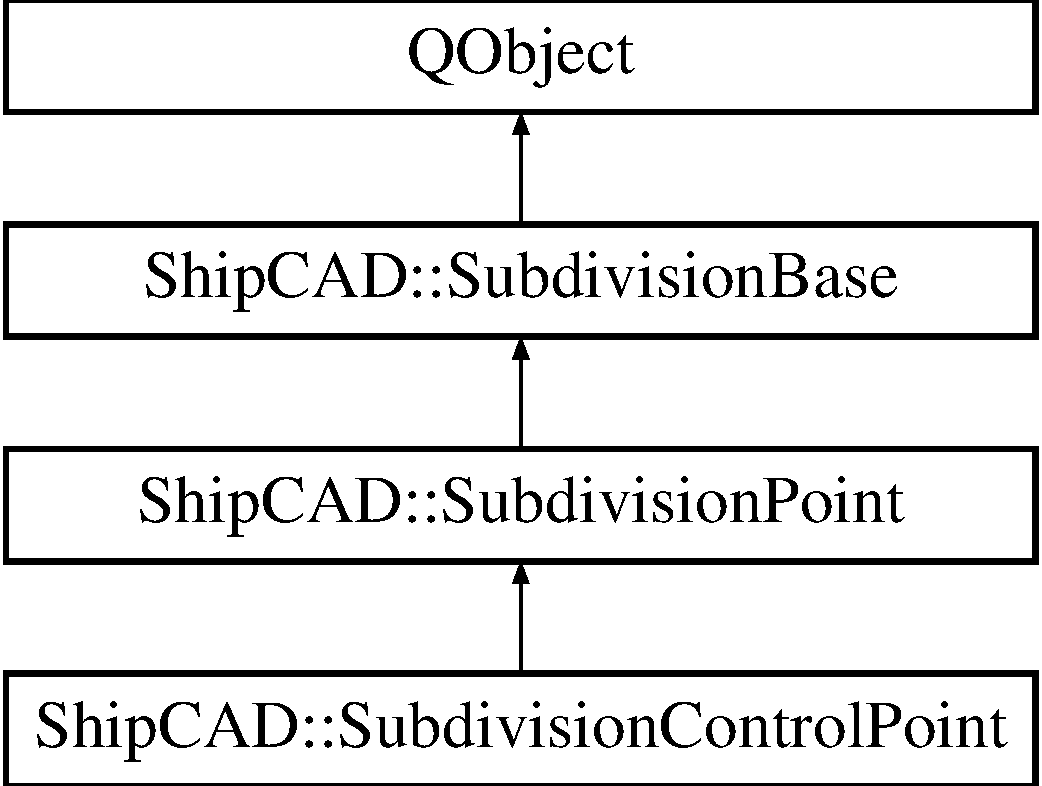
\includegraphics[height=4.000000cm]{classShipCAD_1_1SubdivisionPoint}
\end{center}
\end{figure}
\subsection*{Public Member Functions}
\begin{DoxyCompactItemize}
\item 
\hyperlink{classShipCAD_1_1SubdivisionPoint_aed60af1f2fcbc89bad438a6a131a9f52}{Subdivision\-Point} (\hyperlink{classShipCAD_1_1SubdivisionSurface}{Subdivision\-Surface} $\ast$owner)
\begin{DoxyCompactList}\small\item\em Constructor. \end{DoxyCompactList}\item 
virtual \hyperlink{classShipCAD_1_1SubdivisionPoint_a218f451cd47873d61a4a987ec0cb3e6a}{$\sim$\-Subdivision\-Point} ()
\item 
virtual void \hyperlink{classShipCAD_1_1SubdivisionPoint_aef22d2b6cb48e57ce69652eeb7a69711}{clear} ()
\begin{DoxyCompactList}\small\item\em Reset contents of the Point to default values. \end{DoxyCompactList}\item 
void \hyperlink{classShipCAD_1_1SubdivisionPoint_acd07a93927bf7b6bfe9b4a3233efffdf}{add\-Edge} (\hyperlink{classShipCAD_1_1SubdivisionEdge}{Subdivision\-Edge} $\ast$edge)
\begin{DoxyCompactList}\small\item\em add an Edge \end{DoxyCompactList}\item 
void \hyperlink{classShipCAD_1_1SubdivisionPoint_a077ca16509feb6db73fa40a0098b72b4}{add\-Face} (\hyperlink{classShipCAD_1_1SubdivisionFace}{Subdivision\-Face} $\ast$face)
\begin{DoxyCompactList}\small\item\em add a Face \end{DoxyCompactList}\item 
void \hyperlink{classShipCAD_1_1SubdivisionPoint_a5c1e66b5a28923dca99fe856ce1dff0c}{delete\-Edge} (\hyperlink{classShipCAD_1_1SubdivisionEdge}{Subdivision\-Edge} $\ast$edge)
\begin{DoxyCompactList}\small\item\em delete an Edge \end{DoxyCompactList}\item 
void \hyperlink{classShipCAD_1_1SubdivisionPoint_a7ed94fd26e20c2e30d1f36be6b1a9b29}{delete\-Face} (\hyperlink{classShipCAD_1_1SubdivisionFace}{Subdivision\-Face} $\ast$face)
\begin{DoxyCompactList}\small\item\em delete a Face \end{DoxyCompactList}\item 
void \hyperlink{classShipCAD_1_1SubdivisionPoint_a6037d6e3e78c9cc0d7909a4e55737ad6}{destroy} ()
\item 
float \hyperlink{classShipCAD_1_1SubdivisionPoint_aa07a859d70f97e57fc5318fc64a9d897}{get\-Curvature} ()
\begin{DoxyCompactList}\small\item\em find the curvature of the surface at this point \end{DoxyCompactList}\item 
Q\-Vector3\-D \hyperlink{classShipCAD_1_1SubdivisionPoint_a0c9e47af796dacd9542d065bbd0d0fcf}{averaging} ()
\begin{DoxyCompactList}\small\item\em find the 3\-D coordinates of a point \end{DoxyCompactList}\item 
\hyperlink{classShipCAD_1_1SubdivisionPoint}{Subdivision\-Point} $\ast$ \hyperlink{classShipCAD_1_1SubdivisionPoint_a92632ddbe28fb6901e445b60eab8d3ee}{calculate\-Vertex\-Point} ()
\begin{DoxyCompactList}\small\item\em Create a vertex point. \end{DoxyCompactList}\item 
\hyperlink{namespaceShipCAD_a03171cc921c53a568b778f5131a60deb}{vertex\-\_\-type\-\_\-t} \hyperlink{classShipCAD_1_1SubdivisionPoint_ad6ef4b07ee0d97756395c7bac4082f42}{from\-Int} (int val)
\begin{DoxyCompactList}\small\item\em gets a vertex\-\_\-type\-\_\-t from integer \end{DoxyCompactList}\item 
Q\-Vector3\-D \hyperlink{classShipCAD_1_1SubdivisionPoint_a0cf49d3e181eb00c08119721b33275bc}{get\-Coordinate} ()
\item 
virtual void \hyperlink{classShipCAD_1_1SubdivisionPoint_a98ab99a0ccc4709a40e05b36147c0f55}{set\-Coordinate} (const Q\-Vector3\-D \&val)
\item 
Q\-Vector3\-D \hyperlink{classShipCAD_1_1SubdivisionPoint_a8dd5facd4006480baea4a7f4487094f5}{get\-Normal} ()
\begin{DoxyCompactList}\small\item\em Calculate normal vector. \end{DoxyCompactList}\item 
\hyperlink{classShipCAD_1_1SubdivisionFace}{Subdivision\-Face} $\ast$ \hyperlink{classShipCAD_1_1SubdivisionPoint_a673d2a2c94f52e5523a012959417dcc3}{get\-Face} (size\-\_\-t index)
\item 
\hyperlink{classShipCAD_1_1SubdivisionEdge}{Subdivision\-Edge} $\ast$ \hyperlink{classShipCAD_1_1SubdivisionPoint_a518c4e3dc5de74950c87ff0f733716ba}{get\-Edge} (size\-\_\-t index)
\item 
bool \hyperlink{classShipCAD_1_1SubdivisionPoint_afbcf1244015a92be04faed20163699f7}{is\-Boundary\-Vertex} ()
\item 
virtual size\-\_\-t \hyperlink{classShipCAD_1_1SubdivisionPoint_a8406682549c10ec9e1a184132f6ed2f0}{get\-Index} ()
\begin{DoxyCompactList}\small\item\em index of this point in parent surface \end{DoxyCompactList}\item 
size\-\_\-t \hyperlink{classShipCAD_1_1SubdivisionPoint_a0bc218bf0b1982a6d622535c2653200e}{number\-Of\-Edges} ()
\item 
size\-\_\-t \hyperlink{classShipCAD_1_1SubdivisionPoint_aac07ee9bc037a35a244ab179cf7bd344}{number\-Of\-Faces} ()
\item 
size\-\_\-t \hyperlink{classShipCAD_1_1SubdivisionPoint_afc9659ec83083e7725ce14a12a74d2f0}{number\-Of\-Curves} ()
\item 
bool \hyperlink{classShipCAD_1_1SubdivisionPoint_a6a0b4b628563cda2b2979ce6222e8a20}{is\-Regular\-Point} ()
\item 
Q\-Vector3\-D \hyperlink{classShipCAD_1_1SubdivisionPoint_a0eb743069fe2ee2e99cdf7417b2400d5}{get\-Limit\-Point} ()
\item 
bool \hyperlink{classShipCAD_1_1SubdivisionPoint_a88243019864c79766266cee627671183}{is\-Regular\-N\-U\-R\-B\-S\-Point} (std\-::vector$<$ \hyperlink{classShipCAD_1_1SubdivisionFace}{Subdivision\-Face} $\ast$ $>$ \&faces)
\item 
size\-\_\-t \hyperlink{classShipCAD_1_1SubdivisionPoint_a354475f80700fee46dcb46f8602c5345}{index\-Of\-Face} (\hyperlink{classShipCAD_1_1SubdivisionFace}{Subdivision\-Face} $\ast$face)
\item 
bool \hyperlink{classShipCAD_1_1SubdivisionPoint_ada0d082be616958c024bb1743d392e2f}{has\-Edge} (\hyperlink{classShipCAD_1_1SubdivisionEdge}{Subdivision\-Edge} $\ast$edge)
\item 
bool \hyperlink{classShipCAD_1_1SubdivisionPoint_a720d2fc986ba8a365e8722e0e3e28be5}{has\-Face} (\hyperlink{classShipCAD_1_1SubdivisionFace}{Subdivision\-Face} $\ast$face)
\item 
\hyperlink{namespaceShipCAD_a03171cc921c53a568b778f5131a60deb}{vertex\-\_\-type\-\_\-t} \hyperlink{classShipCAD_1_1SubdivisionPoint_a3ccd55795bf99f25b1ad8f937de9670a}{get\-Vertex\-Type} ()
\item 
void \hyperlink{classShipCAD_1_1SubdivisionPoint_a614259dfa2470bbbd7b8cc73039ad501}{set\-Vertex\-Type} (\hyperlink{namespaceShipCAD_a03171cc921c53a568b778f5131a60deb}{vertex\-\_\-type\-\_\-t} nt)
\item 
virtual void \hyperlink{classShipCAD_1_1SubdivisionPoint_aed72cf5e8dc67e980010d195f3a376a3}{dump} (std\-::ostream \&os, const char $\ast$prefix=\char`\"{}\char`\"{}) const 
\begin{DoxyCompactList}\small\item\em print out the element to a stream \end{DoxyCompactList}\end{DoxyCompactItemize}
\subsection*{Static Public Member Functions}
\begin{DoxyCompactItemize}
\item 
static \hyperlink{classShipCAD_1_1SubdivisionPoint}{Subdivision\-Point} $\ast$ \hyperlink{classShipCAD_1_1SubdivisionPoint_a8e907cca747b0483374d4fdde8eb4ad1}{construct} (\hyperlink{classShipCAD_1_1SubdivisionSurface}{Subdivision\-Surface} $\ast$owner)
\begin{DoxyCompactList}\small\item\em make a point \end{DoxyCompactList}\end{DoxyCompactItemize}
\subsection*{Protected Member Functions}
\begin{DoxyCompactItemize}
\item 
void \hyperlink{classShipCAD_1_1SubdivisionPoint_aa2d85a086268f335eefeaef0b48a96a1}{priv\-\_\-dump} (std\-::ostream \&os, const char $\ast$prefix) const 
\item 
float \hyperlink{classShipCAD_1_1SubdivisionPoint_a72061d495903d8265f33bada30a0c416}{Angle\-\_\-\-V\-V\-\_\-3\-D} (const Q\-Vector3\-D \&p1, const Q\-Vector3\-D \&p2, const Q\-Vector3\-D \&p3)
\end{DoxyCompactItemize}
\subsection*{Protected Attributes}
\begin{DoxyCompactItemize}
\item 
std\-::vector$<$ \hyperlink{classShipCAD_1_1SubdivisionFace}{Subdivision\-Face} $\ast$ $>$ \hyperlink{classShipCAD_1_1SubdivisionPoint_ace13688b5e2ad09c8d3f37cc0eaaaa52}{\-\_\-faces}
\item 
std\-::vector$<$ \hyperlink{classShipCAD_1_1SubdivisionEdge}{Subdivision\-Edge} $\ast$ $>$ \hyperlink{classShipCAD_1_1SubdivisionPoint_a17c5a46dc6c130259e96f49719ef3ee9}{\-\_\-edges}
\item 
Q\-Vector3\-D \hyperlink{classShipCAD_1_1SubdivisionPoint_a42bb8f729c7d79e594bda17f92ddb26b}{\-\_\-coordinate}
\item 
\hyperlink{namespaceShipCAD_a03171cc921c53a568b778f5131a60deb}{vertex\-\_\-type\-\_\-t} \hyperlink{classShipCAD_1_1SubdivisionPoint_a37f4626c2c18a4838f693464d93ad291}{\-\_\-vtype}
\end{DoxyCompactItemize}
\subsection*{Properties}
\begin{DoxyCompactItemize}
\item 
Q\-Vector3\-D \hyperlink{classShipCAD_1_1SubdivisionPoint_a5d39b6f7fe221b5848835a0957702c84}{Coordinate}
\item 
float \hyperlink{classShipCAD_1_1SubdivisionPoint_a30f533619dcb24eb00188772c99564b4}{Curvature}
\item 
bool \hyperlink{classShipCAD_1_1SubdivisionPoint_ad78eae7c6c9a35c329f1137817e10a8d}{Is\-Boundary\-Vertex}
\item 
Q\-Vector3\-D \hyperlink{classShipCAD_1_1SubdivisionPoint_aeaf744ea3deb2bdc55e9e90d3e8b58a2}{Normal}
\item 
size\-\_\-t \hyperlink{classShipCAD_1_1SubdivisionPoint_ad4ec233273e3bc788d2dd6736530d645}{Vertex\-Index}
\item 
\hyperlink{namespaceShipCAD_a03171cc921c53a568b778f5131a60deb}{vertex\-\_\-type\-\_\-t} \hyperlink{classShipCAD_1_1SubdivisionPoint_ab926cef40515c3a4c94a902fb50aa35a}{Vertex\-Type}
\end{DoxyCompactItemize}


\subsection{Detailed Description}
3\-D Point 

Used on boundaries of Faces. 

Definition at line 57 of file subdivpoint.\-h.



\subsection{Constructor \& Destructor Documentation}
\hypertarget{classShipCAD_1_1SubdivisionPoint_aed60af1f2fcbc89bad438a6a131a9f52}{\index{Ship\-C\-A\-D\-::\-Subdivision\-Point@{Ship\-C\-A\-D\-::\-Subdivision\-Point}!Subdivision\-Point@{Subdivision\-Point}}
\index{Subdivision\-Point@{Subdivision\-Point}!ShipCAD::SubdivisionPoint@{Ship\-C\-A\-D\-::\-Subdivision\-Point}}
\subsubsection[{Subdivision\-Point}]{\setlength{\rightskip}{0pt plus 5cm}Subdivision\-Point\-::\-Subdivision\-Point (
\begin{DoxyParamCaption}
\item[{{\bf Subdivision\-Surface} $\ast$}]{owner}
\end{DoxyParamCaption}
)\hspace{0.3cm}{\ttfamily [explicit]}}}\label{classShipCAD_1_1SubdivisionPoint_aed60af1f2fcbc89bad438a6a131a9f52}


Constructor. 

Use the static construct method to create points 

Definition at line 62 of file subdivpoint.\-cpp.

\hypertarget{classShipCAD_1_1SubdivisionPoint_a218f451cd47873d61a4a987ec0cb3e6a}{\index{Ship\-C\-A\-D\-::\-Subdivision\-Point@{Ship\-C\-A\-D\-::\-Subdivision\-Point}!$\sim$\-Subdivision\-Point@{$\sim$\-Subdivision\-Point}}
\index{$\sim$\-Subdivision\-Point@{$\sim$\-Subdivision\-Point}!ShipCAD::SubdivisionPoint@{Ship\-C\-A\-D\-::\-Subdivision\-Point}}
\subsubsection[{$\sim$\-Subdivision\-Point}]{\setlength{\rightskip}{0pt plus 5cm}Subdivision\-Point\-::$\sim$\-Subdivision\-Point (
\begin{DoxyParamCaption}
{}
\end{DoxyParamCaption}
)\hspace{0.3cm}{\ttfamily [virtual]}}}\label{classShipCAD_1_1SubdivisionPoint_a218f451cd47873d61a4a987ec0cb3e6a}


Definition at line 68 of file subdivpoint.\-cpp.



\subsection{Member Function Documentation}
\hypertarget{classShipCAD_1_1SubdivisionPoint_acd07a93927bf7b6bfe9b4a3233efffdf}{\index{Ship\-C\-A\-D\-::\-Subdivision\-Point@{Ship\-C\-A\-D\-::\-Subdivision\-Point}!add\-Edge@{add\-Edge}}
\index{add\-Edge@{add\-Edge}!ShipCAD::SubdivisionPoint@{Ship\-C\-A\-D\-::\-Subdivision\-Point}}
\subsubsection[{add\-Edge}]{\setlength{\rightskip}{0pt plus 5cm}void Subdivision\-Point\-::add\-Edge (
\begin{DoxyParamCaption}
\item[{{\bf Subdivision\-Edge} $\ast$}]{edge}
\end{DoxyParamCaption}
)}}\label{classShipCAD_1_1SubdivisionPoint_acd07a93927bf7b6bfe9b4a3233efffdf}


add an Edge 


\begin{DoxyParams}{Parameters}
{\em edge} & the edge to add to this point \\
\hline
\end{DoxyParams}


Definition at line 301 of file subdivpoint.\-cpp.

\hypertarget{classShipCAD_1_1SubdivisionPoint_a077ca16509feb6db73fa40a0098b72b4}{\index{Ship\-C\-A\-D\-::\-Subdivision\-Point@{Ship\-C\-A\-D\-::\-Subdivision\-Point}!add\-Face@{add\-Face}}
\index{add\-Face@{add\-Face}!ShipCAD::SubdivisionPoint@{Ship\-C\-A\-D\-::\-Subdivision\-Point}}
\subsubsection[{add\-Face}]{\setlength{\rightskip}{0pt plus 5cm}void Subdivision\-Point\-::add\-Face (
\begin{DoxyParamCaption}
\item[{{\bf Subdivision\-Face} $\ast$}]{face}
\end{DoxyParamCaption}
)}}\label{classShipCAD_1_1SubdivisionPoint_a077ca16509feb6db73fa40a0098b72b4}


add a Face 


\begin{DoxyParams}{Parameters}
{\em face} & the face to add to this point \\
\hline
\end{DoxyParams}


Definition at line 307 of file subdivpoint.\-cpp.

\hypertarget{classShipCAD_1_1SubdivisionPoint_a72061d495903d8265f33bada30a0c416}{\index{Ship\-C\-A\-D\-::\-Subdivision\-Point@{Ship\-C\-A\-D\-::\-Subdivision\-Point}!Angle\-\_\-\-V\-V\-\_\-3\-D@{Angle\-\_\-\-V\-V\-\_\-3\-D}}
\index{Angle\-\_\-\-V\-V\-\_\-3\-D@{Angle\-\_\-\-V\-V\-\_\-3\-D}!ShipCAD::SubdivisionPoint@{Ship\-C\-A\-D\-::\-Subdivision\-Point}}
\subsubsection[{Angle\-\_\-\-V\-V\-\_\-3\-D}]{\setlength{\rightskip}{0pt plus 5cm}float Subdivision\-Point\-::\-Angle\-\_\-\-V\-V\-\_\-3\-D (
\begin{DoxyParamCaption}
\item[{const Q\-Vector3\-D \&}]{p1, }
\item[{const Q\-Vector3\-D \&}]{p2, }
\item[{const Q\-Vector3\-D \&}]{p3}
\end{DoxyParamCaption}
)\hspace{0.3cm}{\ttfamily [protected]}}}\label{classShipCAD_1_1SubdivisionPoint_a72061d495903d8265f33bada30a0c416}


Definition at line 118 of file subdivpoint.\-cpp.

\hypertarget{classShipCAD_1_1SubdivisionPoint_a0c9e47af796dacd9542d065bbd0d0fcf}{\index{Ship\-C\-A\-D\-::\-Subdivision\-Point@{Ship\-C\-A\-D\-::\-Subdivision\-Point}!averaging@{averaging}}
\index{averaging@{averaging}!ShipCAD::SubdivisionPoint@{Ship\-C\-A\-D\-::\-Subdivision\-Point}}
\subsubsection[{averaging}]{\setlength{\rightskip}{0pt plus 5cm}Q\-Vector3\-D Subdivision\-Point\-::averaging (
\begin{DoxyParamCaption}
{}
\end{DoxyParamCaption}
)}}\label{classShipCAD_1_1SubdivisionPoint_a0c9e47af796dacd9542d065bbd0d0fcf}


find the 3\-D coordinates of a point 

Get coordinates for this point from faces and edges attached to this point If this is a crease point, then take all opposite end points of edges If this is not a crease point, but all other kinds, then take all points on faces attached to this point, weight them and calculate an average

\begin{DoxyReturn}{Returns}
coordinates of the calculated point 
\end{DoxyReturn}


Definition at line 313 of file subdivpoint.\-cpp.

\hypertarget{classShipCAD_1_1SubdivisionPoint_a92632ddbe28fb6901e445b60eab8d3ee}{\index{Ship\-C\-A\-D\-::\-Subdivision\-Point@{Ship\-C\-A\-D\-::\-Subdivision\-Point}!calculate\-Vertex\-Point@{calculate\-Vertex\-Point}}
\index{calculate\-Vertex\-Point@{calculate\-Vertex\-Point}!ShipCAD::SubdivisionPoint@{Ship\-C\-A\-D\-::\-Subdivision\-Point}}
\subsubsection[{calculate\-Vertex\-Point}]{\setlength{\rightskip}{0pt plus 5cm}{\bf Subdivision\-Point} $\ast$ Subdivision\-Point\-::calculate\-Vertex\-Point (
\begin{DoxyParamCaption}
{}
\end{DoxyParamCaption}
)}}\label{classShipCAD_1_1SubdivisionPoint_a92632ddbe28fb6901e445b60eab8d3ee}


Create a vertex point. 

During the subdivision process, new points are created at the same position as existing points. This method creates a new point at the same position as the old one, also replaces the original point in any curves that contain it with the newly constructed point

\begin{DoxyReturn}{Returns}
new point that is a copy of this one 
\end{DoxyReturn}


Definition at line 396 of file subdivpoint.\-cpp.

\hypertarget{classShipCAD_1_1SubdivisionPoint_aef22d2b6cb48e57ce69652eeb7a69711}{\index{Ship\-C\-A\-D\-::\-Subdivision\-Point@{Ship\-C\-A\-D\-::\-Subdivision\-Point}!clear@{clear}}
\index{clear@{clear}!ShipCAD::SubdivisionPoint@{Ship\-C\-A\-D\-::\-Subdivision\-Point}}
\subsubsection[{clear}]{\setlength{\rightskip}{0pt plus 5cm}void Subdivision\-Point\-::clear (
\begin{DoxyParamCaption}
{}
\end{DoxyParamCaption}
)\hspace{0.3cm}{\ttfamily [virtual]}}}\label{classShipCAD_1_1SubdivisionPoint_aef22d2b6cb48e57ce69652eeb7a69711}


Reset contents of the Point to default values. 



Implements \hyperlink{classShipCAD_1_1SubdivisionBase_a851bb7f1931f9dd6e53b6f9df7b5b352}{Ship\-C\-A\-D\-::\-Subdivision\-Base}.



Definition at line 73 of file subdivpoint.\-cpp.

\hypertarget{classShipCAD_1_1SubdivisionPoint_a8e907cca747b0483374d4fdde8eb4ad1}{\index{Ship\-C\-A\-D\-::\-Subdivision\-Point@{Ship\-C\-A\-D\-::\-Subdivision\-Point}!construct@{construct}}
\index{construct@{construct}!ShipCAD::SubdivisionPoint@{Ship\-C\-A\-D\-::\-Subdivision\-Point}}
\subsubsection[{construct}]{\setlength{\rightskip}{0pt plus 5cm}{\bf Subdivision\-Point} $\ast$ Subdivision\-Point\-::construct (
\begin{DoxyParamCaption}
\item[{{\bf Subdivision\-Surface} $\ast$}]{owner}
\end{DoxyParamCaption}
)\hspace{0.3cm}{\ttfamily [static]}}}\label{classShipCAD_1_1SubdivisionPoint_a8e907cca747b0483374d4fdde8eb4ad1}


make a point 

This doesn't add the point to the parent surface


\begin{DoxyParams}{Parameters}
{\em owner} & surface this point belongs to \\
\hline
\end{DoxyParams}


Definition at line 54 of file subdivpoint.\-cpp.

\hypertarget{classShipCAD_1_1SubdivisionPoint_a5c1e66b5a28923dca99fe856ce1dff0c}{\index{Ship\-C\-A\-D\-::\-Subdivision\-Point@{Ship\-C\-A\-D\-::\-Subdivision\-Point}!delete\-Edge@{delete\-Edge}}
\index{delete\-Edge@{delete\-Edge}!ShipCAD::SubdivisionPoint@{Ship\-C\-A\-D\-::\-Subdivision\-Point}}
\subsubsection[{delete\-Edge}]{\setlength{\rightskip}{0pt plus 5cm}void Subdivision\-Point\-::delete\-Edge (
\begin{DoxyParamCaption}
\item[{{\bf Subdivision\-Edge} $\ast$}]{edge}
\end{DoxyParamCaption}
)}}\label{classShipCAD_1_1SubdivisionPoint_a5c1e66b5a28923dca99fe856ce1dff0c}


delete an Edge 


\begin{DoxyParams}{Parameters}
{\em edge} & the edge to delete from this point \\
\hline
\end{DoxyParams}


Definition at line 409 of file subdivpoint.\-cpp.

\hypertarget{classShipCAD_1_1SubdivisionPoint_a7ed94fd26e20c2e30d1f36be6b1a9b29}{\index{Ship\-C\-A\-D\-::\-Subdivision\-Point@{Ship\-C\-A\-D\-::\-Subdivision\-Point}!delete\-Face@{delete\-Face}}
\index{delete\-Face@{delete\-Face}!ShipCAD::SubdivisionPoint@{Ship\-C\-A\-D\-::\-Subdivision\-Point}}
\subsubsection[{delete\-Face}]{\setlength{\rightskip}{0pt plus 5cm}void Subdivision\-Point\-::delete\-Face (
\begin{DoxyParamCaption}
\item[{{\bf Subdivision\-Face} $\ast$}]{face}
\end{DoxyParamCaption}
)}}\label{classShipCAD_1_1SubdivisionPoint_a7ed94fd26e20c2e30d1f36be6b1a9b29}


delete a Face 


\begin{DoxyParams}{Parameters}
{\em face} & the face to delete from this point \\
\hline
\end{DoxyParams}


Definition at line 417 of file subdivpoint.\-cpp.

\hypertarget{classShipCAD_1_1SubdivisionPoint_a6037d6e3e78c9cc0d7909a4e55737ad6}{\index{Ship\-C\-A\-D\-::\-Subdivision\-Point@{Ship\-C\-A\-D\-::\-Subdivision\-Point}!destroy@{destroy}}
\index{destroy@{destroy}!ShipCAD::SubdivisionPoint@{Ship\-C\-A\-D\-::\-Subdivision\-Point}}
\subsubsection[{destroy}]{\setlength{\rightskip}{0pt plus 5cm}void Ship\-C\-A\-D\-::\-Subdivision\-Point\-::destroy (
\begin{DoxyParamCaption}
{}
\end{DoxyParamCaption}
)}}\label{classShipCAD_1_1SubdivisionPoint_a6037d6e3e78c9cc0d7909a4e55737ad6}
\hypertarget{classShipCAD_1_1SubdivisionPoint_aed72cf5e8dc67e980010d195f3a376a3}{\index{Ship\-C\-A\-D\-::\-Subdivision\-Point@{Ship\-C\-A\-D\-::\-Subdivision\-Point}!dump@{dump}}
\index{dump@{dump}!ShipCAD::SubdivisionPoint@{Ship\-C\-A\-D\-::\-Subdivision\-Point}}
\subsubsection[{dump}]{\setlength{\rightskip}{0pt plus 5cm}void Subdivision\-Point\-::dump (
\begin{DoxyParamCaption}
\item[{std\-::ostream \&}]{os, }
\item[{const char $\ast$}]{prefix = {\ttfamily \char`\"{}\char`\"{}}}
\end{DoxyParamCaption}
) const\hspace{0.3cm}{\ttfamily [virtual]}}}\label{classShipCAD_1_1SubdivisionPoint_aed72cf5e8dc67e980010d195f3a376a3}


print out the element to a stream 


\begin{DoxyParams}{Parameters}
{\em os} & the output stream \\
\hline
{\em prefix} & string to prefix on each line output \\
\hline
\end{DoxyParams}


Reimplemented from \hyperlink{classShipCAD_1_1SubdivisionBase_a7807e64ac8d2acc3da572e03cf0523b6}{Ship\-C\-A\-D\-::\-Subdivision\-Base}.



Reimplemented in \hyperlink{classShipCAD_1_1SubdivisionControlPoint_a4a9d6e45291c27f19f0d76c9b9d19048}{Ship\-C\-A\-D\-::\-Subdivision\-Control\-Point}.



Definition at line 473 of file subdivpoint.\-cpp.

\hypertarget{classShipCAD_1_1SubdivisionPoint_ad6ef4b07ee0d97756395c7bac4082f42}{\index{Ship\-C\-A\-D\-::\-Subdivision\-Point@{Ship\-C\-A\-D\-::\-Subdivision\-Point}!from\-Int@{from\-Int}}
\index{from\-Int@{from\-Int}!ShipCAD::SubdivisionPoint@{Ship\-C\-A\-D\-::\-Subdivision\-Point}}
\subsubsection[{from\-Int}]{\setlength{\rightskip}{0pt plus 5cm}{\bf Ship\-C\-A\-D\-::vertex\-\_\-type\-\_\-t} Subdivision\-Point\-::from\-Int (
\begin{DoxyParamCaption}
\item[{int}]{val}
\end{DoxyParamCaption}
)}}\label{classShipCAD_1_1SubdivisionPoint_ad6ef4b07ee0d97756395c7bac4082f42}


gets a vertex\-\_\-type\-\_\-t from integer 

Returns the vertex\-\_\-type\-\_\-t from an integer, used in serialization


\begin{DoxyParams}{Parameters}
{\em val} & an integer representing vertex type \\
\hline
\end{DoxyParams}
\begin{DoxyReturn}{Returns}
vertex type 
\end{DoxyReturn}


Definition at line 81 of file subdivpoint.\-cpp.

\hypertarget{classShipCAD_1_1SubdivisionPoint_a0cf49d3e181eb00c08119721b33275bc}{\index{Ship\-C\-A\-D\-::\-Subdivision\-Point@{Ship\-C\-A\-D\-::\-Subdivision\-Point}!get\-Coordinate@{get\-Coordinate}}
\index{get\-Coordinate@{get\-Coordinate}!ShipCAD::SubdivisionPoint@{Ship\-C\-A\-D\-::\-Subdivision\-Point}}
\subsubsection[{get\-Coordinate}]{\setlength{\rightskip}{0pt plus 5cm}Q\-Vector3\-D Subdivision\-Point\-::get\-Coordinate (
\begin{DoxyParamCaption}
{}
\end{DoxyParamCaption}
)}}\label{classShipCAD_1_1SubdivisionPoint_a0cf49d3e181eb00c08119721b33275bc}


Definition at line 113 of file subdivpoint.\-cpp.

\hypertarget{classShipCAD_1_1SubdivisionPoint_aa07a859d70f97e57fc5318fc64a9d897}{\index{Ship\-C\-A\-D\-::\-Subdivision\-Point@{Ship\-C\-A\-D\-::\-Subdivision\-Point}!get\-Curvature@{get\-Curvature}}
\index{get\-Curvature@{get\-Curvature}!ShipCAD::SubdivisionPoint@{Ship\-C\-A\-D\-::\-Subdivision\-Point}}
\subsubsection[{get\-Curvature}]{\setlength{\rightskip}{0pt plus 5cm}float Subdivision\-Point\-::get\-Curvature (
\begin{DoxyParamCaption}
{}
\end{DoxyParamCaption}
)}}\label{classShipCAD_1_1SubdivisionPoint_aa07a859d70f97e57fc5318fc64a9d897}


find the curvature of the surface at this point 

For each pair of points attached to faces attached to this point, take the dot product of the triangular face created from that pair and this point. Add these dot products together and convert from radians to degrees

\begin{DoxyReturn}{Returns}
the curvature of the surface at this point 
\end{DoxyReturn}


Definition at line 134 of file subdivpoint.\-cpp.

\hypertarget{classShipCAD_1_1SubdivisionPoint_a518c4e3dc5de74950c87ff0f733716ba}{\index{Ship\-C\-A\-D\-::\-Subdivision\-Point@{Ship\-C\-A\-D\-::\-Subdivision\-Point}!get\-Edge@{get\-Edge}}
\index{get\-Edge@{get\-Edge}!ShipCAD::SubdivisionPoint@{Ship\-C\-A\-D\-::\-Subdivision\-Point}}
\subsubsection[{get\-Edge}]{\setlength{\rightskip}{0pt plus 5cm}{\bf Subdivision\-Edge} $\ast$ Subdivision\-Point\-::get\-Edge (
\begin{DoxyParamCaption}
\item[{size\-\_\-t}]{index}
\end{DoxyParamCaption}
)}}\label{classShipCAD_1_1SubdivisionPoint_a518c4e3dc5de74950c87ff0f733716ba}


Definition at line 94 of file subdivpoint.\-cpp.

\hypertarget{classShipCAD_1_1SubdivisionPoint_a673d2a2c94f52e5523a012959417dcc3}{\index{Ship\-C\-A\-D\-::\-Subdivision\-Point@{Ship\-C\-A\-D\-::\-Subdivision\-Point}!get\-Face@{get\-Face}}
\index{get\-Face@{get\-Face}!ShipCAD::SubdivisionPoint@{Ship\-C\-A\-D\-::\-Subdivision\-Point}}
\subsubsection[{get\-Face}]{\setlength{\rightskip}{0pt plus 5cm}{\bf Subdivision\-Face} $\ast$ Subdivision\-Point\-::get\-Face (
\begin{DoxyParamCaption}
\item[{size\-\_\-t}]{index}
\end{DoxyParamCaption}
)}}\label{classShipCAD_1_1SubdivisionPoint_a673d2a2c94f52e5523a012959417dcc3}


Definition at line 101 of file subdivpoint.\-cpp.

\hypertarget{classShipCAD_1_1SubdivisionPoint_a8406682549c10ec9e1a184132f6ed2f0}{\index{Ship\-C\-A\-D\-::\-Subdivision\-Point@{Ship\-C\-A\-D\-::\-Subdivision\-Point}!get\-Index@{get\-Index}}
\index{get\-Index@{get\-Index}!ShipCAD::SubdivisionPoint@{Ship\-C\-A\-D\-::\-Subdivision\-Point}}
\subsubsection[{get\-Index}]{\setlength{\rightskip}{0pt plus 5cm}size\-\_\-t Subdivision\-Point\-::get\-Index (
\begin{DoxyParamCaption}
{}
\end{DoxyParamCaption}
)\hspace{0.3cm}{\ttfamily [virtual]}}}\label{classShipCAD_1_1SubdivisionPoint_a8406682549c10ec9e1a184132f6ed2f0}


index of this point in parent surface 

\begin{DoxyReturn}{Returns}
the index of this point in parent surface 
\end{DoxyReturn}


Reimplemented in \hyperlink{classShipCAD_1_1SubdivisionControlPoint_a13c569f0894ba6193a3abf894bc4b517}{Ship\-C\-A\-D\-::\-Subdivision\-Control\-Point}.



Definition at line 108 of file subdivpoint.\-cpp.

\hypertarget{classShipCAD_1_1SubdivisionPoint_a0eb743069fe2ee2e99cdf7417b2400d5}{\index{Ship\-C\-A\-D\-::\-Subdivision\-Point@{Ship\-C\-A\-D\-::\-Subdivision\-Point}!get\-Limit\-Point@{get\-Limit\-Point}}
\index{get\-Limit\-Point@{get\-Limit\-Point}!ShipCAD::SubdivisionPoint@{Ship\-C\-A\-D\-::\-Subdivision\-Point}}
\subsubsection[{get\-Limit\-Point}]{\setlength{\rightskip}{0pt plus 5cm}Q\-Vector3\-D Subdivision\-Point\-::get\-Limit\-Point (
\begin{DoxyParamCaption}
{}
\end{DoxyParamCaption}
)}}\label{classShipCAD_1_1SubdivisionPoint_a0eb743069fe2ee2e99cdf7417b2400d5}


Definition at line 218 of file subdivpoint.\-cpp.

\hypertarget{classShipCAD_1_1SubdivisionPoint_a8dd5facd4006480baea4a7f4487094f5}{\index{Ship\-C\-A\-D\-::\-Subdivision\-Point@{Ship\-C\-A\-D\-::\-Subdivision\-Point}!get\-Normal@{get\-Normal}}
\index{get\-Normal@{get\-Normal}!ShipCAD::SubdivisionPoint@{Ship\-C\-A\-D\-::\-Subdivision\-Point}}
\subsubsection[{get\-Normal}]{\setlength{\rightskip}{0pt plus 5cm}Q\-Vector3\-D Subdivision\-Point\-::get\-Normal (
\begin{DoxyParamCaption}
{}
\end{DoxyParamCaption}
)}}\label{classShipCAD_1_1SubdivisionPoint_a8dd5facd4006480baea4a7f4487094f5}


Calculate normal vector. 

Find the surface normal at this point by finding the normal of each face attached to this point, and adding them together.

\begin{DoxyReturn}{Returns}
coordinates of the normal vector 
\end{DoxyReturn}


Definition at line 443 of file subdivpoint.\-cpp.

\hypertarget{classShipCAD_1_1SubdivisionPoint_a3ccd55795bf99f25b1ad8f937de9670a}{\index{Ship\-C\-A\-D\-::\-Subdivision\-Point@{Ship\-C\-A\-D\-::\-Subdivision\-Point}!get\-Vertex\-Type@{get\-Vertex\-Type}}
\index{get\-Vertex\-Type@{get\-Vertex\-Type}!ShipCAD::SubdivisionPoint@{Ship\-C\-A\-D\-::\-Subdivision\-Point}}
\subsubsection[{get\-Vertex\-Type}]{\setlength{\rightskip}{0pt plus 5cm}{\bf vertex\-\_\-type\-\_\-t} Ship\-C\-A\-D\-::\-Subdivision\-Point\-::get\-Vertex\-Type (
\begin{DoxyParamCaption}
{}
\end{DoxyParamCaption}
)\hspace{0.3cm}{\ttfamily [inline]}}}\label{classShipCAD_1_1SubdivisionPoint_a3ccd55795bf99f25b1ad8f937de9670a}


Definition at line 173 of file subdivpoint.\-h.

\hypertarget{classShipCAD_1_1SubdivisionPoint_ada0d082be616958c024bb1743d392e2f}{\index{Ship\-C\-A\-D\-::\-Subdivision\-Point@{Ship\-C\-A\-D\-::\-Subdivision\-Point}!has\-Edge@{has\-Edge}}
\index{has\-Edge@{has\-Edge}!ShipCAD::SubdivisionPoint@{Ship\-C\-A\-D\-::\-Subdivision\-Point}}
\subsubsection[{has\-Edge}]{\setlength{\rightskip}{0pt plus 5cm}bool Subdivision\-Point\-::has\-Edge (
\begin{DoxyParamCaption}
\item[{{\bf Subdivision\-Edge} $\ast$}]{edge}
\end{DoxyParamCaption}
)}}\label{classShipCAD_1_1SubdivisionPoint_ada0d082be616958c024bb1743d392e2f}


Definition at line 433 of file subdivpoint.\-cpp.

\hypertarget{classShipCAD_1_1SubdivisionPoint_a720d2fc986ba8a365e8722e0e3e28be5}{\index{Ship\-C\-A\-D\-::\-Subdivision\-Point@{Ship\-C\-A\-D\-::\-Subdivision\-Point}!has\-Face@{has\-Face}}
\index{has\-Face@{has\-Face}!ShipCAD::SubdivisionPoint@{Ship\-C\-A\-D\-::\-Subdivision\-Point}}
\subsubsection[{has\-Face}]{\setlength{\rightskip}{0pt plus 5cm}bool Subdivision\-Point\-::has\-Face (
\begin{DoxyParamCaption}
\item[{{\bf Subdivision\-Face} $\ast$}]{face}
\end{DoxyParamCaption}
)}}\label{classShipCAD_1_1SubdivisionPoint_a720d2fc986ba8a365e8722e0e3e28be5}


Definition at line 438 of file subdivpoint.\-cpp.

\hypertarget{classShipCAD_1_1SubdivisionPoint_a354475f80700fee46dcb46f8602c5345}{\index{Ship\-C\-A\-D\-::\-Subdivision\-Point@{Ship\-C\-A\-D\-::\-Subdivision\-Point}!index\-Of\-Face@{index\-Of\-Face}}
\index{index\-Of\-Face@{index\-Of\-Face}!ShipCAD::SubdivisionPoint@{Ship\-C\-A\-D\-::\-Subdivision\-Point}}
\subsubsection[{index\-Of\-Face}]{\setlength{\rightskip}{0pt plus 5cm}size\-\_\-t Subdivision\-Point\-::index\-Of\-Face (
\begin{DoxyParamCaption}
\item[{{\bf Subdivision\-Face} $\ast$}]{face}
\end{DoxyParamCaption}
)}}\label{classShipCAD_1_1SubdivisionPoint_a354475f80700fee46dcb46f8602c5345}


Definition at line 425 of file subdivpoint.\-cpp.

\hypertarget{classShipCAD_1_1SubdivisionPoint_afbcf1244015a92be04faed20163699f7}{\index{Ship\-C\-A\-D\-::\-Subdivision\-Point@{Ship\-C\-A\-D\-::\-Subdivision\-Point}!is\-Boundary\-Vertex@{is\-Boundary\-Vertex}}
\index{is\-Boundary\-Vertex@{is\-Boundary\-Vertex}!ShipCAD::SubdivisionPoint@{Ship\-C\-A\-D\-::\-Subdivision\-Point}}
\subsubsection[{is\-Boundary\-Vertex}]{\setlength{\rightskip}{0pt plus 5cm}bool Subdivision\-Point\-::is\-Boundary\-Vertex (
\begin{DoxyParamCaption}
{}
\end{DoxyParamCaption}
)}}\label{classShipCAD_1_1SubdivisionPoint_afbcf1244015a92be04faed20163699f7}


Definition at line 157 of file subdivpoint.\-cpp.

\hypertarget{classShipCAD_1_1SubdivisionPoint_a88243019864c79766266cee627671183}{\index{Ship\-C\-A\-D\-::\-Subdivision\-Point@{Ship\-C\-A\-D\-::\-Subdivision\-Point}!is\-Regular\-N\-U\-R\-B\-S\-Point@{is\-Regular\-N\-U\-R\-B\-S\-Point}}
\index{is\-Regular\-N\-U\-R\-B\-S\-Point@{is\-Regular\-N\-U\-R\-B\-S\-Point}!ShipCAD::SubdivisionPoint@{Ship\-C\-A\-D\-::\-Subdivision\-Point}}
\subsubsection[{is\-Regular\-N\-U\-R\-B\-S\-Point}]{\setlength{\rightskip}{0pt plus 5cm}bool Subdivision\-Point\-::is\-Regular\-N\-U\-R\-B\-S\-Point (
\begin{DoxyParamCaption}
\item[{std\-::vector$<$ {\bf Subdivision\-Face} $\ast$ $>$ \&}]{faces}
\end{DoxyParamCaption}
)}}\label{classShipCAD_1_1SubdivisionPoint_a88243019864c79766266cee627671183}


Definition at line 265 of file subdivpoint.\-cpp.

\hypertarget{classShipCAD_1_1SubdivisionPoint_a6a0b4b628563cda2b2979ce6222e8a20}{\index{Ship\-C\-A\-D\-::\-Subdivision\-Point@{Ship\-C\-A\-D\-::\-Subdivision\-Point}!is\-Regular\-Point@{is\-Regular\-Point}}
\index{is\-Regular\-Point@{is\-Regular\-Point}!ShipCAD::SubdivisionPoint@{Ship\-C\-A\-D\-::\-Subdivision\-Point}}
\subsubsection[{is\-Regular\-Point}]{\setlength{\rightskip}{0pt plus 5cm}bool Subdivision\-Point\-::is\-Regular\-Point (
\begin{DoxyParamCaption}
{}
\end{DoxyParamCaption}
)}}\label{classShipCAD_1_1SubdivisionPoint_a6a0b4b628563cda2b2979ce6222e8a20}


Definition at line 176 of file subdivpoint.\-cpp.

\hypertarget{classShipCAD_1_1SubdivisionPoint_afc9659ec83083e7725ce14a12a74d2f0}{\index{Ship\-C\-A\-D\-::\-Subdivision\-Point@{Ship\-C\-A\-D\-::\-Subdivision\-Point}!number\-Of\-Curves@{number\-Of\-Curves}}
\index{number\-Of\-Curves@{number\-Of\-Curves}!ShipCAD::SubdivisionPoint@{Ship\-C\-A\-D\-::\-Subdivision\-Point}}
\subsubsection[{number\-Of\-Curves}]{\setlength{\rightskip}{0pt plus 5cm}size\-\_\-t Subdivision\-Point\-::number\-Of\-Curves (
\begin{DoxyParamCaption}
{}
\end{DoxyParamCaption}
)}}\label{classShipCAD_1_1SubdivisionPoint_afc9659ec83083e7725ce14a12a74d2f0}


Definition at line 167 of file subdivpoint.\-cpp.

\hypertarget{classShipCAD_1_1SubdivisionPoint_a0bc218bf0b1982a6d622535c2653200e}{\index{Ship\-C\-A\-D\-::\-Subdivision\-Point@{Ship\-C\-A\-D\-::\-Subdivision\-Point}!number\-Of\-Edges@{number\-Of\-Edges}}
\index{number\-Of\-Edges@{number\-Of\-Edges}!ShipCAD::SubdivisionPoint@{Ship\-C\-A\-D\-::\-Subdivision\-Point}}
\subsubsection[{number\-Of\-Edges}]{\setlength{\rightskip}{0pt plus 5cm}size\-\_\-t Ship\-C\-A\-D\-::\-Subdivision\-Point\-::number\-Of\-Edges (
\begin{DoxyParamCaption}
{}
\end{DoxyParamCaption}
)\hspace{0.3cm}{\ttfamily [inline]}}}\label{classShipCAD_1_1SubdivisionPoint_a0bc218bf0b1982a6d622535c2653200e}


Definition at line 164 of file subdivpoint.\-h.

\hypertarget{classShipCAD_1_1SubdivisionPoint_aac07ee9bc037a35a244ab179cf7bd344}{\index{Ship\-C\-A\-D\-::\-Subdivision\-Point@{Ship\-C\-A\-D\-::\-Subdivision\-Point}!number\-Of\-Faces@{number\-Of\-Faces}}
\index{number\-Of\-Faces@{number\-Of\-Faces}!ShipCAD::SubdivisionPoint@{Ship\-C\-A\-D\-::\-Subdivision\-Point}}
\subsubsection[{number\-Of\-Faces}]{\setlength{\rightskip}{0pt plus 5cm}size\-\_\-t Ship\-C\-A\-D\-::\-Subdivision\-Point\-::number\-Of\-Faces (
\begin{DoxyParamCaption}
{}
\end{DoxyParamCaption}
)\hspace{0.3cm}{\ttfamily [inline]}}}\label{classShipCAD_1_1SubdivisionPoint_aac07ee9bc037a35a244ab179cf7bd344}


Definition at line 165 of file subdivpoint.\-h.

\hypertarget{classShipCAD_1_1SubdivisionPoint_aa2d85a086268f335eefeaef0b48a96a1}{\index{Ship\-C\-A\-D\-::\-Subdivision\-Point@{Ship\-C\-A\-D\-::\-Subdivision\-Point}!priv\-\_\-dump@{priv\-\_\-dump}}
\index{priv\-\_\-dump@{priv\-\_\-dump}!ShipCAD::SubdivisionPoint@{Ship\-C\-A\-D\-::\-Subdivision\-Point}}
\subsubsection[{priv\-\_\-dump}]{\setlength{\rightskip}{0pt plus 5cm}void Subdivision\-Point\-::priv\-\_\-dump (
\begin{DoxyParamCaption}
\item[{std\-::ostream \&}]{os, }
\item[{const char $\ast$}]{prefix}
\end{DoxyParamCaption}
) const\hspace{0.3cm}{\ttfamily [protected]}}}\label{classShipCAD_1_1SubdivisionPoint_aa2d85a086268f335eefeaef0b48a96a1}


Definition at line 481 of file subdivpoint.\-cpp.

\hypertarget{classShipCAD_1_1SubdivisionPoint_a98ab99a0ccc4709a40e05b36147c0f55}{\index{Ship\-C\-A\-D\-::\-Subdivision\-Point@{Ship\-C\-A\-D\-::\-Subdivision\-Point}!set\-Coordinate@{set\-Coordinate}}
\index{set\-Coordinate@{set\-Coordinate}!ShipCAD::SubdivisionPoint@{Ship\-C\-A\-D\-::\-Subdivision\-Point}}
\subsubsection[{set\-Coordinate}]{\setlength{\rightskip}{0pt plus 5cm}void Subdivision\-Point\-::set\-Coordinate (
\begin{DoxyParamCaption}
\item[{const Q\-Vector3\-D \&}]{val}
\end{DoxyParamCaption}
)\hspace{0.3cm}{\ttfamily [virtual]}}}\label{classShipCAD_1_1SubdivisionPoint_a98ab99a0ccc4709a40e05b36147c0f55}


Reimplemented in \hyperlink{classShipCAD_1_1SubdivisionControlPoint_a54a5233e02ef34a174c24d5dcf3c6407}{Ship\-C\-A\-D\-::\-Subdivision\-Control\-Point}.



Definition at line 296 of file subdivpoint.\-cpp.

\hypertarget{classShipCAD_1_1SubdivisionPoint_a614259dfa2470bbbd7b8cc73039ad501}{\index{Ship\-C\-A\-D\-::\-Subdivision\-Point@{Ship\-C\-A\-D\-::\-Subdivision\-Point}!set\-Vertex\-Type@{set\-Vertex\-Type}}
\index{set\-Vertex\-Type@{set\-Vertex\-Type}!ShipCAD::SubdivisionPoint@{Ship\-C\-A\-D\-::\-Subdivision\-Point}}
\subsubsection[{set\-Vertex\-Type}]{\setlength{\rightskip}{0pt plus 5cm}void Ship\-C\-A\-D\-::\-Subdivision\-Point\-::set\-Vertex\-Type (
\begin{DoxyParamCaption}
\item[{{\bf vertex\-\_\-type\-\_\-t}}]{nt}
\end{DoxyParamCaption}
)\hspace{0.3cm}{\ttfamily [inline]}}}\label{classShipCAD_1_1SubdivisionPoint_a614259dfa2470bbbd7b8cc73039ad501}


Definition at line 174 of file subdivpoint.\-h.



\subsection{Member Data Documentation}
\hypertarget{classShipCAD_1_1SubdivisionPoint_a42bb8f729c7d79e594bda17f92ddb26b}{\index{Ship\-C\-A\-D\-::\-Subdivision\-Point@{Ship\-C\-A\-D\-::\-Subdivision\-Point}!\-\_\-coordinate@{\-\_\-coordinate}}
\index{\-\_\-coordinate@{\-\_\-coordinate}!ShipCAD::SubdivisionPoint@{Ship\-C\-A\-D\-::\-Subdivision\-Point}}
\subsubsection[{\-\_\-coordinate}]{\setlength{\rightskip}{0pt plus 5cm}Q\-Vector3\-D Ship\-C\-A\-D\-::\-Subdivision\-Point\-::\-\_\-coordinate\hspace{0.3cm}{\ttfamily [protected]}}}\label{classShipCAD_1_1SubdivisionPoint_a42bb8f729c7d79e594bda17f92ddb26b}
3\-D coordinates of this point 

Definition at line 198 of file subdivpoint.\-h.

\hypertarget{classShipCAD_1_1SubdivisionPoint_a17c5a46dc6c130259e96f49719ef3ee9}{\index{Ship\-C\-A\-D\-::\-Subdivision\-Point@{Ship\-C\-A\-D\-::\-Subdivision\-Point}!\-\_\-edges@{\-\_\-edges}}
\index{\-\_\-edges@{\-\_\-edges}!ShipCAD::SubdivisionPoint@{Ship\-C\-A\-D\-::\-Subdivision\-Point}}
\subsubsection[{\-\_\-edges}]{\setlength{\rightskip}{0pt plus 5cm}std\-::vector$<${\bf Subdivision\-Edge}$\ast$$>$ Ship\-C\-A\-D\-::\-Subdivision\-Point\-::\-\_\-edges\hspace{0.3cm}{\ttfamily [protected]}}}\label{classShipCAD_1_1SubdivisionPoint_a17c5a46dc6c130259e96f49719ef3ee9}
list of edges attached to this point 

Definition at line 197 of file subdivpoint.\-h.

\hypertarget{classShipCAD_1_1SubdivisionPoint_ace13688b5e2ad09c8d3f37cc0eaaaa52}{\index{Ship\-C\-A\-D\-::\-Subdivision\-Point@{Ship\-C\-A\-D\-::\-Subdivision\-Point}!\-\_\-faces@{\-\_\-faces}}
\index{\-\_\-faces@{\-\_\-faces}!ShipCAD::SubdivisionPoint@{Ship\-C\-A\-D\-::\-Subdivision\-Point}}
\subsubsection[{\-\_\-faces}]{\setlength{\rightskip}{0pt plus 5cm}std\-::vector$<${\bf Subdivision\-Face}$\ast$$>$ Ship\-C\-A\-D\-::\-Subdivision\-Point\-::\-\_\-faces\hspace{0.3cm}{\ttfamily [protected]}}}\label{classShipCAD_1_1SubdivisionPoint_ace13688b5e2ad09c8d3f37cc0eaaaa52}
list of faces attached to this point 

Definition at line 196 of file subdivpoint.\-h.

\hypertarget{classShipCAD_1_1SubdivisionPoint_a37f4626c2c18a4838f693464d93ad291}{\index{Ship\-C\-A\-D\-::\-Subdivision\-Point@{Ship\-C\-A\-D\-::\-Subdivision\-Point}!\-\_\-vtype@{\-\_\-vtype}}
\index{\-\_\-vtype@{\-\_\-vtype}!ShipCAD::SubdivisionPoint@{Ship\-C\-A\-D\-::\-Subdivision\-Point}}
\subsubsection[{\-\_\-vtype}]{\setlength{\rightskip}{0pt plus 5cm}{\bf vertex\-\_\-type\-\_\-t} Ship\-C\-A\-D\-::\-Subdivision\-Point\-::\-\_\-vtype\hspace{0.3cm}{\ttfamily [protected]}}}\label{classShipCAD_1_1SubdivisionPoint_a37f4626c2c18a4838f693464d93ad291}
vertex type of this point 

Definition at line 199 of file subdivpoint.\-h.



\subsection{Property Documentation}
\hypertarget{classShipCAD_1_1SubdivisionPoint_a5d39b6f7fe221b5848835a0957702c84}{\index{Ship\-C\-A\-D\-::\-Subdivision\-Point@{Ship\-C\-A\-D\-::\-Subdivision\-Point}!Coordinate@{Coordinate}}
\index{Coordinate@{Coordinate}!ShipCAD::SubdivisionPoint@{Ship\-C\-A\-D\-::\-Subdivision\-Point}}
\subsubsection[{Coordinate}]{\setlength{\rightskip}{0pt plus 5cm}Q\-Vector3\-D Ship\-C\-A\-D\-::\-Subdivision\-Point\-::\-Coordinate\hspace{0.3cm}{\ttfamily [read]}, {\ttfamily [write]}}}\label{classShipCAD_1_1SubdivisionPoint_a5d39b6f7fe221b5848835a0957702c84}


Definition at line 60 of file subdivpoint.\-h.

\hypertarget{classShipCAD_1_1SubdivisionPoint_a30f533619dcb24eb00188772c99564b4}{\index{Ship\-C\-A\-D\-::\-Subdivision\-Point@{Ship\-C\-A\-D\-::\-Subdivision\-Point}!Curvature@{Curvature}}
\index{Curvature@{Curvature}!ShipCAD::SubdivisionPoint@{Ship\-C\-A\-D\-::\-Subdivision\-Point}}
\subsubsection[{Curvature}]{\setlength{\rightskip}{0pt plus 5cm}float Ship\-C\-A\-D\-::\-Subdivision\-Point\-::\-Curvature\hspace{0.3cm}{\ttfamily [read]}}}\label{classShipCAD_1_1SubdivisionPoint_a30f533619dcb24eb00188772c99564b4}


Definition at line 61 of file subdivpoint.\-h.

\hypertarget{classShipCAD_1_1SubdivisionPoint_ad78eae7c6c9a35c329f1137817e10a8d}{\index{Ship\-C\-A\-D\-::\-Subdivision\-Point@{Ship\-C\-A\-D\-::\-Subdivision\-Point}!Is\-Boundary\-Vertex@{Is\-Boundary\-Vertex}}
\index{Is\-Boundary\-Vertex@{Is\-Boundary\-Vertex}!ShipCAD::SubdivisionPoint@{Ship\-C\-A\-D\-::\-Subdivision\-Point}}
\subsubsection[{Is\-Boundary\-Vertex}]{\setlength{\rightskip}{0pt plus 5cm}bool Ship\-C\-A\-D\-::\-Subdivision\-Point\-::\-Is\-Boundary\-Vertex\hspace{0.3cm}{\ttfamily [read]}}}\label{classShipCAD_1_1SubdivisionPoint_ad78eae7c6c9a35c329f1137817e10a8d}


Definition at line 62 of file subdivpoint.\-h.

\hypertarget{classShipCAD_1_1SubdivisionPoint_aeaf744ea3deb2bdc55e9e90d3e8b58a2}{\index{Ship\-C\-A\-D\-::\-Subdivision\-Point@{Ship\-C\-A\-D\-::\-Subdivision\-Point}!Normal@{Normal}}
\index{Normal@{Normal}!ShipCAD::SubdivisionPoint@{Ship\-C\-A\-D\-::\-Subdivision\-Point}}
\subsubsection[{Normal}]{\setlength{\rightskip}{0pt plus 5cm}Q\-Vector3\-D Ship\-C\-A\-D\-::\-Subdivision\-Point\-::\-Normal\hspace{0.3cm}{\ttfamily [read]}}}\label{classShipCAD_1_1SubdivisionPoint_aeaf744ea3deb2bdc55e9e90d3e8b58a2}


Definition at line 63 of file subdivpoint.\-h.

\hypertarget{classShipCAD_1_1SubdivisionPoint_ad4ec233273e3bc788d2dd6736530d645}{\index{Ship\-C\-A\-D\-::\-Subdivision\-Point@{Ship\-C\-A\-D\-::\-Subdivision\-Point}!Vertex\-Index@{Vertex\-Index}}
\index{Vertex\-Index@{Vertex\-Index}!ShipCAD::SubdivisionPoint@{Ship\-C\-A\-D\-::\-Subdivision\-Point}}
\subsubsection[{Vertex\-Index}]{\setlength{\rightskip}{0pt plus 5cm}size\-\_\-t Ship\-C\-A\-D\-::\-Subdivision\-Point\-::\-Vertex\-Index\hspace{0.3cm}{\ttfamily [read]}}}\label{classShipCAD_1_1SubdivisionPoint_ad4ec233273e3bc788d2dd6736530d645}


Definition at line 64 of file subdivpoint.\-h.

\hypertarget{classShipCAD_1_1SubdivisionPoint_ab926cef40515c3a4c94a902fb50aa35a}{\index{Ship\-C\-A\-D\-::\-Subdivision\-Point@{Ship\-C\-A\-D\-::\-Subdivision\-Point}!Vertex\-Type@{Vertex\-Type}}
\index{Vertex\-Type@{Vertex\-Type}!ShipCAD::SubdivisionPoint@{Ship\-C\-A\-D\-::\-Subdivision\-Point}}
\subsubsection[{Vertex\-Type}]{\setlength{\rightskip}{0pt plus 5cm}{\bf vertex\-\_\-type\-\_\-t} Ship\-C\-A\-D\-::\-Subdivision\-Point\-::\-Vertex\-Type\hspace{0.3cm}{\ttfamily [read]}, {\ttfamily [write]}}}\label{classShipCAD_1_1SubdivisionPoint_ab926cef40515c3a4c94a902fb50aa35a}


Definition at line 65 of file subdivpoint.\-h.



The documentation for this class was generated from the following files\-:\begin{DoxyCompactItemize}
\item 
Ship\-C\-A\-Dlib/\hyperlink{subdivpoint_8h}{subdivpoint.\-h}\item 
Ship\-C\-A\-Dlib/\hyperlink{subdivpoint_8cpp}{subdivpoint.\-cpp}\end{DoxyCompactItemize}

\hypertarget{classShipCAD_1_1SubdivisionSurface}{\section{Ship\-C\-A\-D\-:\-:Subdivision\-Surface Class Reference}
\label{classShipCAD_1_1SubdivisionSurface}\index{Ship\-C\-A\-D\-::\-Subdivision\-Surface@{Ship\-C\-A\-D\-::\-Subdivision\-Surface}}
}


{\ttfamily \#include $<$subdivsurface.\-h$>$}

Inheritance diagram for Ship\-C\-A\-D\-:\-:Subdivision\-Surface\-:\begin{figure}[H]
\begin{center}
\leavevmode
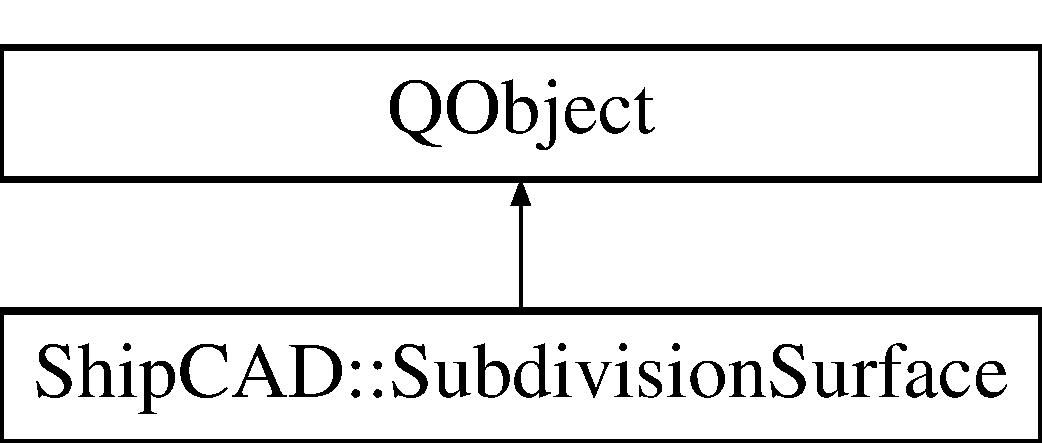
\includegraphics[height=2.000000cm]{classShipCAD_1_1SubdivisionSurface}
\end{center}
\end{figure}
\subsection*{Public Types}
\begin{DoxyCompactItemize}
\item 
typedef std\-::vector\\*
$<$ std\-::vector\\*
$<$ \hyperlink{classShipCAD_1_1SubdivisionControlFace}{Subdivision\-Control\-Face} $\ast$ $>$ $>$ \hyperlink{classShipCAD_1_1SubdivisionSurface_a26a7d7b71acd662b1014ab39af4ee343}{face\-\_\-grid\-\_\-t}
\item 
typedef std\-::vector\\*
$<$ std\-::vector\\*
$<$ \hyperlink{classShipCAD_1_1SubdivisionPoint}{Subdivision\-Point} $\ast$ $>$ $>$ \hyperlink{classShipCAD_1_1SubdivisionSurface_a69d4a3ca038ee247d0abcffa6125df95}{grid\-\_\-t}
\item 
typedef std\-::vector\\*
$<$ std\-::vector\\*
$<$ \hyperlink{classShipCAD_1_1SubdivisionControlPoint}{Subdivision\-Control\-Point} $\ast$ $>$ $>$ \hyperlink{classShipCAD_1_1SubdivisionSurface_ae53cacefe98ce33992a05f941f4ff4ee}{control\-\_\-grid\-\_\-t}
\item 
typedef std\-::vector\\*
$<$ std\-::vector$<$ Q\-Vector3\-D $>$ $>$ \hyperlink{classShipCAD_1_1SubdivisionSurface_a8ed657cb7d4cd34662bd2d3e949d3e3b}{coordinate\-\_\-grid\-\_\-t}
\end{DoxyCompactItemize}
\subsection*{Signals}
\begin{DoxyCompactItemize}
\item 
void \hyperlink{classShipCAD_1_1SubdivisionSurface_a5598e484d5deddfa353ddc4f02d3b004}{changed\-Layer\-Data} ()
\item 
void \hyperlink{classShipCAD_1_1SubdivisionSurface_aad7f3abd89252d503b7d21ca306436d4}{change\-Active\-Layer} ()
\item 
void \hyperlink{classShipCAD_1_1SubdivisionSurface_a83bf6f16944165a6e96a1f9387b783e7}{select\-Item} (\hyperlink{classShipCAD_1_1SubdivisionBase}{Subdivision\-Base} $\ast$)
\end{DoxyCompactItemize}
\subsection*{Public Member Functions}
\begin{DoxyCompactItemize}
\item 
\hyperlink{classShipCAD_1_1SubdivisionSurface_a507ea9cd5354e1d14fe24d52da505934}{Subdivision\-Surface} ()
\item 
virtual \hyperlink{classShipCAD_1_1SubdivisionSurface_a4f1b66a4d9e9f8ac3dbd956e2113a594}{$\sim$\-Subdivision\-Surface} ()
\item 
virtual void \hyperlink{classShipCAD_1_1SubdivisionSurface_a80ab3bd6372a8465d69f71034a353e06}{clear} ()
\item 
void \hyperlink{classShipCAD_1_1SubdivisionSurface_a13cfd2714344c9b85aad8d123538db48}{initialize} (size\-\_\-t point\-\_\-start, size\-\_\-t edge\-\_\-start)
\item 
void \hyperlink{classShipCAD_1_1SubdivisionSurface_a259856fc21f2bc1eebbc52f10dd59469}{rebuild} ()
\item 
void \hyperlink{classShipCAD_1_1SubdivisionSurface_ad140279118fab3343a6aee5e544814ec}{assemble\-Faces\-To\-Patches} (std\-::vector$<$ \hyperlink{classShipCAD_1_1SubdivisionLayer}{Subdivision\-Layer} $\ast$ $>$ \&layers, \hyperlink{namespaceShipCAD_aaba70dc1c80dc540bef320cb9b720a20}{assemble\-\_\-mode\-\_\-t} mode, std\-::vector$<$ \hyperlink{classShipCAD_1_1SubdivisionFace}{Subdivision\-Face} $\ast$ $>$ \&assembled\-Patches, size\-\_\-t \&n\-Assembled)
\item 
void \hyperlink{classShipCAD_1_1SubdivisionSurface_a3aa7c4fd1fa84170a59e6c0549573c92}{calculate\-Gauss\-Curvature} ()
\item 
void \hyperlink{classShipCAD_1_1SubdivisionSurface_a2a984cc9ae8c78153113552cfb6321d5}{clear\-Selection} ()
\item 
void \hyperlink{classShipCAD_1_1SubdivisionSurface_a1deabf43f6a24c34a58889d0361b0959}{convert\-To\-Grid} (\hyperlink{classShipCAD_1_1SubdivisionSurface_a26a7d7b71acd662b1014ab39af4ee343}{face\-\_\-grid\-\_\-t} \&input, \hyperlink{classShipCAD_1_1SubdivisionSurface_a69d4a3ca038ee247d0abcffa6125df95}{grid\-\_\-t} \&grid)
\item 
void \hyperlink{classShipCAD_1_1SubdivisionSurface_aa0460120d8a093682ca352a47affdb87}{edge\-Connect} ()
\item 
void \hyperlink{classShipCAD_1_1SubdivisionSurface_abc1cf0168290242dfbe5dd0d178fa7cb}{extents} (Q\-Vector3\-D \&min, Q\-Vector3\-D \&max)
\item 
void \hyperlink{classShipCAD_1_1SubdivisionSurface_ac19570e1402deab738d2231d6bec9650}{extrude\-Edges} (std\-::vector$<$ \hyperlink{classShipCAD_1_1SubdivisionControlEdge}{Subdivision\-Control\-Edge} $\ast$ $>$ \&edges, const Q\-Vector3\-D \&direction)
\item 
void \hyperlink{classShipCAD_1_1SubdivisionSurface_a576a4d43e01ca50782ba724f63f1b2bd}{calculate\-Intersections} (const \hyperlink{classShipCAD_1_1Plane}{Plane} \&plane, std\-::vector$<$ \hyperlink{classShipCAD_1_1SubdivisionControlFace}{Subdivision\-Control\-Face} $\ast$ $>$ \&faces, std\-::vector$<$ \hyperlink{classShipCAD_1_1Spline}{Spline} $\ast$ $>$ \&destination)
\item 
void \hyperlink{classShipCAD_1_1SubdivisionSurface_a17dccf4965b49427d345bd5acce897c5}{extract\-All\-Edge\-Loops} (std\-::vector$<$ std\-::vector$<$ \hyperlink{classShipCAD_1_1SubdivisionPoint}{Subdivision\-Point} $\ast$ $>$ $>$ \&destination)
\item 
void \hyperlink{classShipCAD_1_1SubdivisionSurface_af62ba549d058dfddd4bfa1b69a577220}{extract\-Points\-From\-Faces} (std\-::vector$<$ \hyperlink{classShipCAD_1_1SubdivisionFace}{Subdivision\-Face} $\ast$ $>$ \&selectedfaces, std\-::vector$<$ \hyperlink{classShipCAD_1_1SubdivisionControlPoint}{Subdivision\-Control\-Point} $\ast$ $>$ \&points, size\-\_\-t \&lockedpoints)
\item 
void \hyperlink{classShipCAD_1_1SubdivisionSurface_af0f0d7bb979c8c8ba04b9be26e7cfe30}{extract\-Points\-From\-Selection} (std\-::vector$<$ \hyperlink{classShipCAD_1_1SubdivisionControlPoint}{Subdivision\-Control\-Point} $\ast$ $>$ \&selectedpoints, size\-\_\-t \&lockedpoints)
\item 
void \hyperlink{classShipCAD_1_1SubdivisionSurface_aa193fd28425e9846908479615e7c5bf9}{import\-Grid} (\hyperlink{classShipCAD_1_1SubdivisionSurface_a8ed657cb7d4cd34662bd2d3e949d3e3b}{coordinate\-\_\-grid\-\_\-t} \&points, \hyperlink{classShipCAD_1_1SubdivisionLayer}{Subdivision\-Layer} $\ast$layer)
\item 
bool \hyperlink{classShipCAD_1_1SubdivisionSurface_ab7191008f7ec3ef34b578b27e4340927}{intersect\-Plane} (const \hyperlink{classShipCAD_1_1Plane}{Plane} \&plane, bool hydrostatics\-\_\-layers\-\_\-only, std\-::vector$<$ \hyperlink{classShipCAD_1_1Spline}{Spline} $\ast$ $>$ \&destination)
\item 
void \hyperlink{classShipCAD_1_1SubdivisionSurface_ada26b740ea1f317763b6ecd372f13ea2}{insert\-Plane} (const \hyperlink{classShipCAD_1_1Plane}{Plane} \&plane, bool add\-\_\-curves)
\item 
void \hyperlink{classShipCAD_1_1SubdivisionSurface_ad9970c667fa8e33ff8b35eb6a48b6a2e}{subdivide} ()
\item 
void \hyperlink{classShipCAD_1_1SubdivisionSurface_a99bda5b49300775eda1df60451412686}{selection\-Delete} ()
\item 
size\-\_\-t \hyperlink{classShipCAD_1_1SubdivisionSurface_a771f0f1881a2da57dde8cb88a8fc9059}{number\-Of\-Locked\-Points} ()
\item 
size\-\_\-t \hyperlink{classShipCAD_1_1SubdivisionSurface_a2583bc0013b5725ac0902062d1c8bcea}{number\-Of\-Selected\-Locked\-Points} ()
\item 
size\-\_\-t \hyperlink{classShipCAD_1_1SubdivisionSurface_a404ffc0c4d13a3a00edb83ad439ee59e}{number\-Of\-Points} ()
\item 
size\-\_\-t \hyperlink{classShipCAD_1_1SubdivisionSurface_a1bde01d6b5972c302ad387cf1247f0fa}{index\-Of\-Point} (\hyperlink{classShipCAD_1_1SubdivisionPoint}{Subdivision\-Point} $\ast$pt)
\item 
\hyperlink{classShipCAD_1_1SubdivisionPoint}{Subdivision\-Point} $\ast$ \hyperlink{classShipCAD_1_1SubdivisionSurface_af07192c8cfc3429ad6da80a1da802a6c}{get\-Point} (size\-\_\-t index)
\item 
void \hyperlink{classShipCAD_1_1SubdivisionSurface_a4117039bfd819cb28ab5cb04296fdcd7}{delete\-Point} (\hyperlink{classShipCAD_1_1SubdivisionPoint}{Subdivision\-Point} $\ast$pt)
\item 
size\-\_\-t \hyperlink{classShipCAD_1_1SubdivisionSurface_a4e184650893ca2ac7e367778ec70c45f}{number\-Of\-Control\-Points} ()
\item 
size\-\_\-t \hyperlink{classShipCAD_1_1SubdivisionSurface_ae0dda53669e5767da6434b3e2f751916}{index\-Of\-Control\-Point} (\hyperlink{classShipCAD_1_1SubdivisionControlPoint}{Subdivision\-Control\-Point} $\ast$pt)
\item 
bool \hyperlink{classShipCAD_1_1SubdivisionSurface_a62abb29703f608a75559452d25db9a33}{has\-Control\-Point} (\hyperlink{classShipCAD_1_1SubdivisionControlPoint}{Subdivision\-Control\-Point} $\ast$pt)
\item 
void \hyperlink{classShipCAD_1_1SubdivisionSurface_aa20b9227481180329e03de8897c52933}{remove\-Control\-Point} (\hyperlink{classShipCAD_1_1SubdivisionControlPoint}{Subdivision\-Control\-Point} $\ast$pt)
\item 
\hyperlink{classShipCAD_1_1SubdivisionControlPoint}{Subdivision\-Control\-Point} $\ast$ \hyperlink{classShipCAD_1_1SubdivisionSurface_a8aa8d3fdfc5e81ba4a39858a69228652}{get\-Control\-Point} (size\-\_\-t index)
\item 
\hyperlink{classShipCAD_1_1SubdivisionControlPoint}{Subdivision\-Control\-Point} $\ast$ \hyperlink{classShipCAD_1_1SubdivisionSurface_af644edd0d4ba993dbab280f036b37171}{add\-Control\-Point} (const Q\-Vector3\-D \&pt)
\item 
void \hyperlink{classShipCAD_1_1SubdivisionSurface_a7ac8b717bcb728da2334cc2f16c8b428}{add\-Control\-Point} (\hyperlink{classShipCAD_1_1SubdivisionControlPoint}{Subdivision\-Control\-Point} $\ast$pt)
\item 
\hyperlink{classShipCAD_1_1SubdivisionControlPoint}{Subdivision\-Control\-Point} $\ast$ \hyperlink{classShipCAD_1_1SubdivisionSurface_a7eccf33cb39ef12f56553352da34da62}{add\-Control\-Point} ()
\item 
void \hyperlink{classShipCAD_1_1SubdivisionSurface_ad4f874132a137e89a39e60572748dab0}{delete\-Control\-Point} (\hyperlink{classShipCAD_1_1SubdivisionControlPoint}{Subdivision\-Control\-Point} $\ast$point)
\item 
size\-\_\-t \hyperlink{classShipCAD_1_1SubdivisionSurface_ac15e844f2feb644d71b1de3a886f6970}{number\-Of\-Selected\-Control\-Points} ()
\item 
bool \hyperlink{classShipCAD_1_1SubdivisionSurface_aafd696ac2c5353ac5593acdbe8b1fb2e}{has\-Selected\-Control\-Point} (\hyperlink{classShipCAD_1_1SubdivisionControlPoint}{Subdivision\-Control\-Point} $\ast$pt)
\item 
void \hyperlink{classShipCAD_1_1SubdivisionSurface_a65cc43d93da8ed72af631e893057c773}{set\-Selected\-Control\-Point} (\hyperlink{classShipCAD_1_1SubdivisionControlPoint}{Subdivision\-Control\-Point} $\ast$pt)
\item 
void \hyperlink{classShipCAD_1_1SubdivisionSurface_a5be891c06dc5e441511fbdb73d71efeb}{remove\-Selected\-Control\-Point} (\hyperlink{classShipCAD_1_1SubdivisionControlPoint}{Subdivision\-Control\-Point} $\ast$pt)
\item 
size\-\_\-t \hyperlink{classShipCAD_1_1SubdivisionSurface_a74c607d9835c69a00b7730fad5384037}{number\-Of\-Edges} ()
\item 
size\-\_\-t \hyperlink{classShipCAD_1_1SubdivisionSurface_aa3d68eacb2fafd9dab6d40c3230ed991}{index\-Of\-Edge} (\hyperlink{classShipCAD_1_1SubdivisionEdge}{Subdivision\-Edge} $\ast$edge)
\item 
\hyperlink{classShipCAD_1_1SubdivisionEdge}{Subdivision\-Edge} $\ast$ \hyperlink{classShipCAD_1_1SubdivisionSurface_a67e69fc54ca38627596efc49b6d82e7f}{get\-Edge} (size\-\_\-t index)
\item 
\hyperlink{classShipCAD_1_1SubdivisionEdge}{Subdivision\-Edge} $\ast$ \hyperlink{classShipCAD_1_1SubdivisionSurface_adfdeabdc19eb55a7ba4ab0b607207300}{edge\-Exists} (\hyperlink{classShipCAD_1_1SubdivisionPoint}{Subdivision\-Point} $\ast$p1, \hyperlink{classShipCAD_1_1SubdivisionPoint}{Subdivision\-Point} $\ast$p2)
\item 
void \hyperlink{classShipCAD_1_1SubdivisionSurface_abb5beb9a6fc413e8d713e18fb39bf2ba}{delete\-Edge} (\hyperlink{classShipCAD_1_1SubdivisionEdge}{Subdivision\-Edge} $\ast$edge)
\item 
size\-\_\-t \hyperlink{classShipCAD_1_1SubdivisionSurface_a2fd710a2e2fa0272b8c8f498b8fc4f56}{number\-Of\-Control\-Edges} ()
\item 
size\-\_\-t \hyperlink{classShipCAD_1_1SubdivisionSurface_ae2f4e931f0134f8637e0aa769dba1d32}{index\-Of\-Control\-Edge} (\hyperlink{classShipCAD_1_1SubdivisionControlEdge}{Subdivision\-Control\-Edge} $\ast$edge)
\item 
\hyperlink{classShipCAD_1_1SubdivisionControlEdge}{Subdivision\-Control\-Edge} $\ast$ \hyperlink{classShipCAD_1_1SubdivisionSurface_ac7d6762dc83f1f114c1d7f4e67d8f8eb}{get\-Control\-Edge} (size\-\_\-t index)
\item 
bool \hyperlink{classShipCAD_1_1SubdivisionSurface_a9856bef9e5b2de9be4a3118fa80d0f16}{has\-Control\-Edge} (\hyperlink{classShipCAD_1_1SubdivisionControlEdge}{Subdivision\-Control\-Edge} $\ast$edge)
\item 
\hyperlink{classShipCAD_1_1SubdivisionControlEdge}{Subdivision\-Control\-Edge} $\ast$ \hyperlink{classShipCAD_1_1SubdivisionSurface_a976358235d20a0fdc83248948bb9cf48}{add\-Control\-Edge} (\hyperlink{classShipCAD_1_1SubdivisionPoint}{Subdivision\-Point} $\ast$sp, \hyperlink{classShipCAD_1_1SubdivisionPoint}{Subdivision\-Point} $\ast$ep)
\item 
void \hyperlink{classShipCAD_1_1SubdivisionSurface_acfec50abf57a44ed47038ecc55f5a600}{add\-Control\-Edge} (\hyperlink{classShipCAD_1_1SubdivisionControlEdge}{Subdivision\-Control\-Edge} $\ast$edge)
\item 
\hyperlink{classShipCAD_1_1SubdivisionControlEdge}{Subdivision\-Control\-Edge} $\ast$ \hyperlink{classShipCAD_1_1SubdivisionSurface_a6a89be4440e3adfcb0b14c164db891ae}{control\-Edge\-Exists} (\hyperlink{classShipCAD_1_1SubdivisionPoint}{Subdivision\-Point} $\ast$p1, \hyperlink{classShipCAD_1_1SubdivisionPoint}{Subdivision\-Point} $\ast$p2)
\item 
void \hyperlink{classShipCAD_1_1SubdivisionSurface_a3aac4d6c8ad638234f88fb8b1ffa00cb}{remove\-Control\-Edge} (\hyperlink{classShipCAD_1_1SubdivisionControlEdge}{Subdivision\-Control\-Edge} $\ast$edge)
\item 
void \hyperlink{classShipCAD_1_1SubdivisionSurface_ae45fc2694977c8fbae54ac2e0e067d1f}{delete\-Control\-Edge} (\hyperlink{classShipCAD_1_1SubdivisionControlEdge}{Subdivision\-Control\-Edge} $\ast$edge)
\item 
void \hyperlink{classShipCAD_1_1SubdivisionSurface_a975c97ca338eb2aaaa3dcc0640611a95}{isolate\-Edges} (std\-::vector$<$ \hyperlink{classShipCAD_1_1SubdivisionControlEdge}{Subdivision\-Control\-Edge} $\ast$ $>$ \&input, std\-::vector$<$ std\-::vector$<$ \hyperlink{classShipCAD_1_1SubdivisionControlPoint}{Subdivision\-Control\-Point} $\ast$ $>$ $>$ \&sorted)
\item 
size\-\_\-t \hyperlink{classShipCAD_1_1SubdivisionSurface_a28f394042987ccc30d947ddd98a62574}{number\-Of\-Selected\-Control\-Edges} ()
\item 
void \hyperlink{classShipCAD_1_1SubdivisionSurface_ae1ceb8323935d0734fe4dc9c324aca16}{set\-Selected\-Control\-Edge} (\hyperlink{classShipCAD_1_1SubdivisionControlEdge}{Subdivision\-Control\-Edge} $\ast$edge)
\item 
void \hyperlink{classShipCAD_1_1SubdivisionSurface_a579077d742f9afc4e1d4ad20ef5a2184}{remove\-Selected\-Control\-Edge} (\hyperlink{classShipCAD_1_1SubdivisionControlEdge}{Subdivision\-Control\-Edge} $\ast$edge)
\item 
bool \hyperlink{classShipCAD_1_1SubdivisionSurface_a3f7856ea95b0c881a1171845c1dc817e}{has\-Selected\-Control\-Edge} (\hyperlink{classShipCAD_1_1SubdivisionControlEdge}{Subdivision\-Control\-Edge} $\ast$edge)
\item 
size\-\_\-t \hyperlink{classShipCAD_1_1SubdivisionSurface_a9f67bb8bbd3a8f61a2b4abacc0cf10e4}{number\-Of\-Faces} ()
\item 
void \hyperlink{classShipCAD_1_1SubdivisionSurface_abf11847b9df1bc590c6c51d292430dd5}{clear\-Faces} ()
\item 
size\-\_\-t \hyperlink{classShipCAD_1_1SubdivisionSurface_a2fb486ba7285a42ae7fdab6e6c289fc5}{number\-Of\-Control\-Faces} ()
\item 
size\-\_\-t \hyperlink{classShipCAD_1_1SubdivisionSurface_aee61b8795a0f16c47df83f0ef0abd2e7}{index\-Of\-Control\-Face} (\hyperlink{classShipCAD_1_1SubdivisionControlFace}{Subdivision\-Control\-Face} $\ast$face)
\item 
\hyperlink{classShipCAD_1_1SubdivisionControlFace}{Subdivision\-Control\-Face} $\ast$ \hyperlink{classShipCAD_1_1SubdivisionSurface_a392f052a12118427919b910e99663d92}{get\-Control\-Face} (size\-\_\-t index)
\item 
\hyperlink{classShipCAD_1_1SubdivisionControlFace}{Subdivision\-Control\-Face} $\ast$ \hyperlink{classShipCAD_1_1SubdivisionSurface_a536574cc453e4790a769a3e7d47b7ff1}{get\-Control\-Face} (\hyperlink{classShipCAD_1_1SubdivisionPoint}{Subdivision\-Point} $\ast$p1, \hyperlink{classShipCAD_1_1SubdivisionPoint}{Subdivision\-Point} $\ast$p2, \hyperlink{classShipCAD_1_1SubdivisionPoint}{Subdivision\-Point} $\ast$p3, \hyperlink{classShipCAD_1_1SubdivisionPoint}{Subdivision\-Point} $\ast$p4)
\item 
bool \hyperlink{classShipCAD_1_1SubdivisionSurface_ad6e00013faf6c373bfc1421adb941ba4}{has\-Control\-Face} (\hyperlink{classShipCAD_1_1SubdivisionControlFace}{Subdivision\-Control\-Face} $\ast$face)
\item 
void \hyperlink{classShipCAD_1_1SubdivisionSurface_abbbb7422a86771451034d2fb7a76bb26}{add\-Control\-Face} (\hyperlink{classShipCAD_1_1SubdivisionControlFace}{Subdivision\-Control\-Face} $\ast$face)
\item 
\hyperlink{classShipCAD_1_1SubdivisionControlFace}{Subdivision\-Control\-Face} $\ast$ \hyperlink{classShipCAD_1_1SubdivisionSurface_a7c83a514f43b868b5fa286f3bc05a41e}{add\-Control\-Face} (std\-::vector$<$ Q\-Vector3\-D $>$ \&points)
\item 
\hyperlink{classShipCAD_1_1SubdivisionControlFace}{Subdivision\-Control\-Face} $\ast$ \hyperlink{classShipCAD_1_1SubdivisionSurface_a957b534788873921249cd1cc058b9d7e}{add\-Control\-Face} (std\-::vector$<$ \hyperlink{classShipCAD_1_1SubdivisionControlPoint}{Subdivision\-Control\-Point} $\ast$ $>$ \&points, bool check\-\_\-edges)
\item 
\hyperlink{classShipCAD_1_1SubdivisionControlFace}{Subdivision\-Control\-Face} $\ast$ \hyperlink{classShipCAD_1_1SubdivisionSurface_a07d8ca69ed3d45f6e54407fcca8264b2}{add\-Control\-Face} (std\-::vector$<$ \hyperlink{classShipCAD_1_1SubdivisionControlPoint}{Subdivision\-Control\-Point} $\ast$ $>$ \&points, bool check\-\_\-edges, \hyperlink{classShipCAD_1_1SubdivisionLayer}{Subdivision\-Layer} $\ast$layer)
\item 
void \hyperlink{classShipCAD_1_1SubdivisionSurface_a9cce3014753c0b74517b1747a80f6c2c}{remove\-Control\-Face} (\hyperlink{classShipCAD_1_1SubdivisionControlFace}{Subdivision\-Control\-Face} $\ast$face)
\item 
void \hyperlink{classShipCAD_1_1SubdivisionSurface_a394c490440fb20c37abfc2f38d6e50fd}{delete\-Control\-Face} (\hyperlink{classShipCAD_1_1SubdivisionControlFace}{Subdivision\-Control\-Face} $\ast$face)
\item 
size\-\_\-t \hyperlink{classShipCAD_1_1SubdivisionSurface_a084a7f6b226f8d5991f7c99607d0ddb0}{number\-Of\-Selected\-Control\-Faces} ()
\item 
void \hyperlink{classShipCAD_1_1SubdivisionSurface_ab21694a435e0c0dd6139de28ae543254}{set\-Selected\-Control\-Face} (\hyperlink{classShipCAD_1_1SubdivisionControlFace}{Subdivision\-Control\-Face} $\ast$face)
\item 
void \hyperlink{classShipCAD_1_1SubdivisionSurface_aef09d950b0970bd825a984effeee6224}{remove\-Selected\-Control\-Face} (\hyperlink{classShipCAD_1_1SubdivisionControlFace}{Subdivision\-Control\-Face} $\ast$face)
\item 
bool \hyperlink{classShipCAD_1_1SubdivisionSurface_aab0e513988645c868676831ae0093a25}{has\-Selected\-Control\-Face} (\hyperlink{classShipCAD_1_1SubdivisionControlFace}{Subdivision\-Control\-Face} $\ast$face)
\item 
size\-\_\-t \hyperlink{classShipCAD_1_1SubdivisionSurface_a076772817afcb44926a3d898754261ce}{number\-Of\-Control\-Curves} ()
\item 
size\-\_\-t \hyperlink{classShipCAD_1_1SubdivisionSurface_a83c515916e068cbed7f7afd7bf11d84a}{index\-Of\-Control\-Curve} (\hyperlink{classShipCAD_1_1SubdivisionControlCurve}{Subdivision\-Control\-Curve} $\ast$curve)
\item 
\hyperlink{classShipCAD_1_1SubdivisionControlCurve}{Subdivision\-Control\-Curve} $\ast$ \hyperlink{classShipCAD_1_1SubdivisionSurface_a732c53d18277a4093ff7df12c0b08634}{get\-Control\-Curve} (size\-\_\-t index)
\item 
bool \hyperlink{classShipCAD_1_1SubdivisionSurface_acc30feeff1a889b9b291dcab3987b30a}{has\-Control\-Curve} (\hyperlink{classShipCAD_1_1SubdivisionControlCurve}{Subdivision\-Control\-Curve} $\ast$curve)
\item 
void \hyperlink{classShipCAD_1_1SubdivisionSurface_aa01ccc2ce7417960ca13075e38eb98e6}{add\-Control\-Curve} (\hyperlink{classShipCAD_1_1SubdivisionControlCurve}{Subdivision\-Control\-Curve} $\ast$curve)
\item 
void \hyperlink{classShipCAD_1_1SubdivisionSurface_abd51f7744580144550fabc086ea991b4}{remove\-Control\-Curve} (\hyperlink{classShipCAD_1_1SubdivisionControlCurve}{Subdivision\-Control\-Curve} $\ast$curve)
\item 
size\-\_\-t \hyperlink{classShipCAD_1_1SubdivisionSurface_a174e6e97b72c037693369e3716522ced}{number\-Of\-Selected\-Control\-Curves} ()
\item 
void \hyperlink{classShipCAD_1_1SubdivisionSurface_a5614a6ea5e1b67ec516328d64574cd9e}{set\-Selected\-Control\-Curve} (\hyperlink{classShipCAD_1_1SubdivisionControlCurve}{Subdivision\-Control\-Curve} $\ast$curve)
\item 
void \hyperlink{classShipCAD_1_1SubdivisionSurface_a1666628c8232ba11d386641fa7980ed7}{remove\-Selected\-Control\-Curve} (\hyperlink{classShipCAD_1_1SubdivisionControlCurve}{Subdivision\-Control\-Curve} $\ast$curve)
\item 
bool \hyperlink{classShipCAD_1_1SubdivisionSurface_acdfbfb4870bf517cd075fdf51a0de997}{has\-Selected\-Control\-Curve} (\hyperlink{classShipCAD_1_1SubdivisionControlCurve}{Subdivision\-Control\-Curve} $\ast$curve)
\item 
size\-\_\-t \hyperlink{classShipCAD_1_1SubdivisionSurface_ad9d00dfc848975306c43305e13e57ebe}{number\-Of\-Layers} ()
\item 
size\-\_\-t \hyperlink{classShipCAD_1_1SubdivisionSurface_accb1e8604e44f491f84e9fb77d1ab5c7}{index\-Of\-Layer} (\hyperlink{classShipCAD_1_1SubdivisionLayer}{Subdivision\-Layer} $\ast$layer)
\item 
\hyperlink{classShipCAD_1_1SubdivisionLayer}{Subdivision\-Layer} $\ast$ \hyperlink{classShipCAD_1_1SubdivisionSurface_a24b230e51a0c5fb3e7f51d0e2340eb9f}{get\-Layer} (size\-\_\-t index)
\item 
\hyperlink{classShipCAD_1_1SubdivisionLayer}{Subdivision\-Layer} $\ast$ \hyperlink{classShipCAD_1_1SubdivisionSurface_a490d7a6fef79ba56fd36395208b46ba5}{get\-Active\-Layer} ()
\item 
void \hyperlink{classShipCAD_1_1SubdivisionSurface_a69bafa71111e562a52a089be99b47871}{set\-Active\-Layer} (\hyperlink{classShipCAD_1_1SubdivisionLayer}{Subdivision\-Layer} $\ast$layer)
\item 
bool \hyperlink{classShipCAD_1_1SubdivisionSurface_aef9fe9a74054b54292f7f64e0589743c}{has\-Layer} (\hyperlink{classShipCAD_1_1SubdivisionLayer}{Subdivision\-Layer} $\ast$layer)
\item 
void \hyperlink{classShipCAD_1_1SubdivisionSurface_a3f0dac49106056562a8b675c61918abe}{delete\-Layer} (\hyperlink{classShipCAD_1_1SubdivisionLayer}{Subdivision\-Layer} $\ast$layer)
\item 
size\-\_\-t \hyperlink{classShipCAD_1_1SubdivisionSurface_a46966d7372d20e563fddc48d6bbcab8a}{last\-Used\-Layer\-I\-D} ()
\item 
void \hyperlink{classShipCAD_1_1SubdivisionSurface_aa72a8cf7c5bddaaf24ec41ad3480fe70}{set\-Last\-Used\-Layer\-I\-D} (size\-\_\-t newid)
\item 
size\-\_\-t \hyperlink{classShipCAD_1_1SubdivisionSurface_a3af3a30b53d867b2b25f9ac9290a264a}{request\-New\-Layer\-I\-D} ()
\item 
\hyperlink{classShipCAD_1_1SubdivisionLayer}{Subdivision\-Layer} $\ast$ \hyperlink{classShipCAD_1_1SubdivisionSurface_a5bf8f452664e17dae636d4b66a66eba9}{add\-New\-Layer} ()
\item 
bool \hyperlink{classShipCAD_1_1SubdivisionSurface_a54b74c879ff3782b264e27a8d4fab368}{is\-Build} ()
\item 
void \hyperlink{classShipCAD_1_1SubdivisionSurface_aec5073750762d1f8c3ab2107a742f4a5}{set\-Build} (bool val)
\item 
\hyperlink{namespaceShipCAD_a4a9d1acfd6a2e1e9078a5dcc36f0c817}{subdiv\-\_\-mode\-\_\-t} \hyperlink{classShipCAD_1_1SubdivisionSurface_a77ac47de5e6323271f45be37223fe82b}{get\-Subdivision\-Mode} ()
\item 
void \hyperlink{classShipCAD_1_1SubdivisionSurface_a048dce00d2ff87aa5b31319ea41f565a}{set\-Subdivision\-Mode} (\hyperlink{namespaceShipCAD_a4a9d1acfd6a2e1e9078a5dcc36f0c817}{subdiv\-\_\-mode\-\_\-t} val)
\item 
void \hyperlink{classShipCAD_1_1SubdivisionSurface_a53271216c1be89154c08d2b2841f9a60}{set\-Desired\-Subdivision\-Level} (int val)
\item 
bool \hyperlink{classShipCAD_1_1SubdivisionSurface_aa6e07e073f76fb31d013103c8709f923}{is\-Gauss\-Curvature\-Calculated} ()
\item 
float \hyperlink{classShipCAD_1_1SubdivisionSurface_a8dfd63bd3bd8ddf35491b12003a8b7ce}{get\-Curvature\-Scale} ()
\item 
void \hyperlink{classShipCAD_1_1SubdivisionSurface_af0de3c1d862ddb2466effbcff0189845}{set\-Curvature\-Scale} (float val)
\item 
float \hyperlink{classShipCAD_1_1SubdivisionSurface_ae511889be6115d7461808eda144947a8}{get\-Min\-Gaus\-Curvature} ()
\item 
float \hyperlink{classShipCAD_1_1SubdivisionSurface_a5189aba41418c44faae76b39284917c2}{get\-Max\-Gaus\-Curvature} ()
\item 
const \hyperlink{classShipCAD_1_1Plane}{Plane} \& \hyperlink{classShipCAD_1_1SubdivisionSurface_a5f4515130c512327b01e6aea577d0876}{get\-Waterline\-Plane} ()
\item 
void \hyperlink{classShipCAD_1_1SubdivisionSurface_ae063d1a2be4e227aaefb8a3578d3f52f}{set\-Waterline\-Plane} (const \hyperlink{classShipCAD_1_1Plane}{Plane} \&val)
\item 
float \hyperlink{classShipCAD_1_1SubdivisionSurface_a8b33594cec15c0ec7aa03eb9d53327bb}{get\-Mainframe\-Location} ()
\item 
void \hyperlink{classShipCAD_1_1SubdivisionSurface_a81d5637d3b405da5975eb8e86d058bcd}{set\-Mainframe\-Location} (float val)
\item 
int \hyperlink{classShipCAD_1_1SubdivisionSurface_a521c5ea29e765a0cf7bc0ec0268b499c}{get\-Control\-Point\-Size} ()
\item 
bool \hyperlink{classShipCAD_1_1SubdivisionSurface_ac7c4656b21e0aaa01525be5b7be84024}{show\-Curvature} ()
\item 
bool \hyperlink{classShipCAD_1_1SubdivisionSurface_adfb570208c96bf8bc3426a43fda5fe9f}{shade\-Under\-Water} ()
\item 
bool \hyperlink{classShipCAD_1_1SubdivisionSurface_a1886c21030a3c5c85797603d2d00c906}{show\-Control\-Net} ()
\item 
bool \hyperlink{classShipCAD_1_1SubdivisionSurface_ac94824bf3a085f9785bc49e659077156}{show\-Control\-Curves} ()
\item 
bool \hyperlink{classShipCAD_1_1SubdivisionSurface_a84834b65650ff350e993c00dccabab46}{show\-Interior\-Edges} ()
\item 
bool \hyperlink{classShipCAD_1_1SubdivisionSurface_a94d284672cca1fb619ef5c064bcd175b}{draw\-Mirror} ()
\item 
bool \hyperlink{classShipCAD_1_1SubdivisionSurface_a57a2abe37fef2cee7ca6c15ae5173672}{show\-Normals} ()
\item 
void \hyperlink{classShipCAD_1_1SubdivisionSurface_abf6fe62614aadf1cdd4f26fb4d3fc441}{set\-Show\-Curvature} (bool val)
\item 
void \hyperlink{classShipCAD_1_1SubdivisionSurface_a797d9b728f794b7f2fc61f1c51dacc06}{set\-Shade\-Under\-Water} (bool val)
\item 
void \hyperlink{classShipCAD_1_1SubdivisionSurface_af5380f1a7932b23a5fbf400c85542381}{set\-Show\-Control\-Net} (bool val)
\item 
void \hyperlink{classShipCAD_1_1SubdivisionSurface_aabf54bc152176697a82c0eb6e47f5981}{set\-Show\-Control\-Curves} (bool val)
\item 
void \hyperlink{classShipCAD_1_1SubdivisionSurface_a5a4e5acd1bfc4d845d28513dd2dbc0cd}{set\-Show\-Interior\-Edges} (bool val)
\item 
void \hyperlink{classShipCAD_1_1SubdivisionSurface_a3605a409a102a18714e9ad7d028e7f33}{set\-Draw\-Mirror} (bool val)
\item 
void \hyperlink{classShipCAD_1_1SubdivisionSurface_a678530145785bd366316b35d2bd0ab67}{set\-Show\-Normals} (bool val)
\item 
Q\-Color \hyperlink{classShipCAD_1_1SubdivisionSurface_a4d307277e2a96d86b3d3e7788c2aac0a}{get\-Selected\-Color} ()
\item 
Q\-Color \hyperlink{classShipCAD_1_1SubdivisionSurface_a50b5868db7d2c5d6cce75fa2b52be60f}{get\-Crease\-Edge\-Color} ()
\item 
Q\-Color \hyperlink{classShipCAD_1_1SubdivisionSurface_a40dd77bdff5cf86b4a6eca7ff5a2e643}{get\-Edge\-Color} ()
\item 
Q\-Color \hyperlink{classShipCAD_1_1SubdivisionSurface_ac3131c3badeb6b11cb8a5ec5ceef0961}{get\-Leak\-Color} ()
\item 
Q\-Color \hyperlink{classShipCAD_1_1SubdivisionSurface_afdf406376421eb43a34f53392fbcf5b1}{get\-Regular\-Point\-Color} ()
\item 
Q\-Color \hyperlink{classShipCAD_1_1SubdivisionSurface_af64e951c070d6c88f70c399bc13809d1}{get\-Corner\-Point\-Color} ()
\item 
Q\-Color \hyperlink{classShipCAD_1_1SubdivisionSurface_ac355dfe572889755c24d1c8cd3145aea}{get\-Dart\-Point\-Color} ()
\item 
Q\-Color \hyperlink{classShipCAD_1_1SubdivisionSurface_a6aad1f3725f8033bb85403a01c252006}{get\-Crease\-Color} ()
\item 
Q\-Color \hyperlink{classShipCAD_1_1SubdivisionSurface_a82c8cb1c6c448be7554bcb42e0099660}{get\-Crease\-Point\-Color} ()
\item 
Q\-Color \hyperlink{classShipCAD_1_1SubdivisionSurface_a5b35353f739d224d8aa40ff19333ba98}{get\-Control\-Curve\-Color} ()
\item 
Q\-Color \hyperlink{classShipCAD_1_1SubdivisionSurface_a2a5e9c50d43e72829e02a8c0be31c260}{get\-Layer\-Color} ()
\item 
Q\-Color \hyperlink{classShipCAD_1_1SubdivisionSurface_aa39747141685b52d3987cf6c9f4e2aa8}{get\-Curvature\-Color} ()
\item 
void \hyperlink{classShipCAD_1_1SubdivisionSurface_a6e6254ecc6fcbdadf1ff4f646caa1d59}{save\-Binary} (\hyperlink{classShipCAD_1_1FileBuffer}{File\-Buffer} \&destination)
\item 
void \hyperlink{classShipCAD_1_1SubdivisionSurface_ac8ad644e0c19ac180fd4a7368fa410a6}{load\-Binary} (\hyperlink{classShipCAD_1_1FileBuffer}{File\-Buffer} \&source)
\item 
void \hyperlink{classShipCAD_1_1SubdivisionSurface_a489eed6508bb376170fa7926d2b7dc10}{load\-From\-Stream} (size\-\_\-t \&lineno, std\-::vector$<$ Q\-String $>$ \&strings)
\item 
void \hyperlink{classShipCAD_1_1SubdivisionSurface_add8d612c82f170869f81042520f62499}{load\-V\-R\-M\-L\-File} (const Q\-String \&filename)
\item 
void \hyperlink{classShipCAD_1_1SubdivisionSurface_a958a2af5d8d06ccf1aa3ac4e812cb1be}{export\-Fe\-F\-File} (std\-::vector$<$ Q\-String $>$ \&strings)
\item 
void \hyperlink{classShipCAD_1_1SubdivisionSurface_af5e99c578032b83916f5c06591cbf459}{import\-Fe\-F\-File} (std\-::vector$<$ Q\-String $>$ \&strings, size\-\_\-t \&lineno)
\item 
void \hyperlink{classShipCAD_1_1SubdivisionSurface_ac6a4c0542b17b1b50edb57ea5c0f28ec}{export\-Obj\-File} (bool export\-\_\-control\-\_\-net, std\-::vector$<$ Q\-String $>$ \&strings)
\item 
void \hyperlink{classShipCAD_1_1SubdivisionSurface_a51d2d07423cc53fc98012f07ed9525bc}{save\-To\-Stream} (std\-::vector$<$ Q\-String $>$ \&strings)
\item 
virtual void \hyperlink{classShipCAD_1_1SubdivisionSurface_acfe9cc964dbe05105486b43f2dc6fc4f}{draw} (\hyperlink{classShipCAD_1_1Viewport}{Viewport} \&vp)
\item 
virtual void \hyperlink{classShipCAD_1_1SubdivisionSurface_a6ed961bbb7ca5fe94ec5566109d9b015}{dump} (std\-::ostream \&os, const char $\ast$prefix=\char`\"{}\char`\"{}) const 
\item 
boost\-::pool \& \hyperlink{classShipCAD_1_1SubdivisionSurface_a49109b80a26f29ad52ac109574cf4d5a}{get\-Control\-Point\-Pool} ()
\item 
boost\-::pool \& \hyperlink{classShipCAD_1_1SubdivisionSurface_aa9ed4c00847b5c04f99b27f754df481b}{get\-Control\-Edge\-Pool} ()
\item 
boost\-::pool \& \hyperlink{classShipCAD_1_1SubdivisionSurface_ab9199097e998971add79f7dccbd262c3}{get\-Control\-Face\-Pool} ()
\item 
boost\-::pool \& \hyperlink{classShipCAD_1_1SubdivisionSurface_a647c0e4a20cfd823cc578431c2799c04}{get\-Control\-Curve\-Pool} ()
\item 
boost\-::pool \& \hyperlink{classShipCAD_1_1SubdivisionSurface_a7e80bac4f91557a620fc1843f77b9953}{get\-Layer\-Pool} ()
\item 
boost\-::pool \& \hyperlink{classShipCAD_1_1SubdivisionSurface_a8a8dbbc32fcdc5a08c462cd86c224649}{get\-Point\-Pool} ()
\item 
boost\-::pool \& \hyperlink{classShipCAD_1_1SubdivisionSurface_a2bffb2bf9575d934e18ed5087f8d2996}{get\-Edge\-Pool} ()
\item 
boost\-::pool \& \hyperlink{classShipCAD_1_1SubdivisionSurface_a3fcdae8e54e98938de00dfa4229d8aa8}{get\-Face\-Pool} ()
\end{DoxyCompactItemize}
\subsection*{Protected Member Functions}
\begin{DoxyCompactItemize}
\item 
void \hyperlink{classShipCAD_1_1SubdivisionSurface_a5c88eb988cc6a439242264bc54a6e3e1}{priv\-\_\-dump} (std\-::ostream \&os, const char $\ast$prefix) const 
\item 
\hyperlink{classShipCAD_1_1SubdivisionControlPoint}{Subdivision\-Control\-Point} $\ast$ \hyperlink{classShipCAD_1_1SubdivisionSurface_a251b711125d50aa51875451976e8a8d7}{new\-Control\-Point} (const Q\-Vector3\-D \&p)
\item 
void \hyperlink{classShipCAD_1_1SubdivisionSurface_a3163cfd01e0454ecb9dbb088dc76fbc6}{find\-Attached\-Faces} (std\-::vector$<$ \hyperlink{classShipCAD_1_1SubdivisionControlFace}{Subdivision\-Control\-Face} $\ast$ $>$ \&found\-\_\-list, std\-::vector$<$ \hyperlink{classShipCAD_1_1SubdivisionControlFace}{Subdivision\-Control\-Face} $\ast$ $>$ \&todo\-\_\-list, \hyperlink{classShipCAD_1_1SubdivisionControlFace}{Subdivision\-Control\-Face} $\ast$face)
\item 
bool \hyperlink{classShipCAD_1_1SubdivisionSurface_a5b6204bb0648f2e85cbf07ffbac4bd42}{valid\-Face} (\hyperlink{classShipCAD_1_1SubdivisionFace}{Subdivision\-Face} $\ast$face, std\-::vector$<$ \hyperlink{classShipCAD_1_1SubdivisionFace}{Subdivision\-Face} $\ast$ $>$ \&faces, std\-::vector$<$ \hyperlink{classShipCAD_1_1SubdivisionFace}{Subdivision\-Face} $\ast$ $>$ \&tmpfaces)
\item 
void \hyperlink{classShipCAD_1_1SubdivisionSurface_ac322d8008ea13bc3ca3fd1baeab7e1b3}{do\-Assemble} (\hyperlink{classShipCAD_1_1SubdivisionSurface_a69d4a3ca038ee247d0abcffa6125df95}{grid\-\_\-t} \&grid, size\-\_\-t \&cols, size\-\_\-t \&rows, std\-::vector$<$ \hyperlink{classShipCAD_1_1SubdivisionFace}{Subdivision\-Face} $\ast$ $>$ \&faces)
\item 
void \hyperlink{classShipCAD_1_1SubdivisionSurface_a2b270b878bb810d51bd7adf689db5366}{sort\-Edges} (std\-::vector$<$ \hyperlink{classShipCAD_1_1SubdivisionEdge}{Subdivision\-Edge} $\ast$ $>$ \&edges)
\item 
std\-::vector$<$ \hyperlink{classShipCAD_1_1SubdivisionPoint}{Subdivision\-Point} $\ast$ $>$ \hyperlink{classShipCAD_1_1SubdivisionSurface_abbabb02057a2e66d2a37ec84696788e9}{sort\-Edges} (bool always\-\_\-true, std\-::vector$<$ \hyperlink{classShipCAD_1_1SubdivisionEdge}{Subdivision\-Edge} $\ast$ $>$ \&edges)
\item 
std\-::vector\\*
$<$ \hyperlink{classShipCAD_1_1SubdivisionControlPoint}{Subdivision\-Control\-Point} $\ast$ $>$ \hyperlink{classShipCAD_1_1SubdivisionSurface_a8650bf95c9eb2de0e0b1342bfacbe82a}{sort\-Edges} (std\-::vector$<$ \hyperlink{classShipCAD_1_1SubdivisionControlEdge}{Subdivision\-Control\-Edge} $\ast$ $>$ \&edges)
\end{DoxyCompactItemize}
\subsection*{Protected Attributes}
\begin{DoxyCompactItemize}
\item 
bool \hyperlink{classShipCAD_1_1SubdivisionSurface_ad360f009ac9c27aad0a88b2df7070414}{\-\_\-build}
\item 
bool \hyperlink{classShipCAD_1_1SubdivisionSurface_ab9bb374cf1368b4a2c779f953bca88a8}{\-\_\-show\-\_\-control\-\_\-net}
\item 
bool \hyperlink{classShipCAD_1_1SubdivisionSurface_a828f85ee49e1481e95f61b919070842c}{\-\_\-initialized}
\item 
bool \hyperlink{classShipCAD_1_1SubdivisionSurface_a4458d02152bd97495938586c89e6d9e2}{\-\_\-show\-\_\-interior\-\_\-edges}
\item 
bool \hyperlink{classShipCAD_1_1SubdivisionSurface_a4ee73ae98bddfe1819419afd1d5ba029}{\-\_\-draw\-\_\-mirror}
\item 
bool \hyperlink{classShipCAD_1_1SubdivisionSurface_ac3294d41679de31e588d603e3428565e}{\-\_\-shade\-\_\-under\-\_\-water}
\item 
bool \hyperlink{classShipCAD_1_1SubdivisionSurface_a0cc840743e7afcd136ab864ace158a17}{\-\_\-show\-\_\-normals}
\item 
bool \hyperlink{classShipCAD_1_1SubdivisionSurface_abe2167085eac50c986b074635b610462}{\-\_\-show\-\_\-curvature}
\item 
bool \hyperlink{classShipCAD_1_1SubdivisionSurface_ae240b2177e0af0bd1512c94b524f22dd}{\-\_\-show\-\_\-control\-\_\-curves}
\item 
\hyperlink{namespaceShipCAD_a4a9d1acfd6a2e1e9078a5dcc36f0c817}{subdiv\-\_\-mode\-\_\-t} \hyperlink{classShipCAD_1_1SubdivisionSurface_a0af5c881dfa24574962f42d80da997ee}{\-\_\-subdivision\-\_\-mode}
\item 
int \hyperlink{classShipCAD_1_1SubdivisionSurface_aeec20f09be87e6d57d88f903853ca96f}{\-\_\-desired\-\_\-subdiv\-\_\-level}
\item 
int \hyperlink{classShipCAD_1_1SubdivisionSurface_a9e5424746eced5d0a06ccbe4055bd06f}{\-\_\-current\-\_\-subdiv\-\_\-level}
\item 
int \hyperlink{classShipCAD_1_1SubdivisionSurface_a7ad820b9d312c8ecde939b5345690d35}{\-\_\-control\-\_\-point\-\_\-size}
\item 
float \hyperlink{classShipCAD_1_1SubdivisionSurface_acf241b41a8ca897306decbbab8e44c69}{\-\_\-curvature\-\_\-scale}
\item 
float \hyperlink{classShipCAD_1_1SubdivisionSurface_ac343c30f7e4e6a5926fdfed7da3f9385}{\-\_\-min\-\_\-gaus\-\_\-curvature}
\item 
float \hyperlink{classShipCAD_1_1SubdivisionSurface_a1658374385131656d359ff373d2cb08c}{\-\_\-max\-\_\-gaus\-\_\-curvature}
\item 
float \hyperlink{classShipCAD_1_1SubdivisionSurface_a3ea08aa45ad221a1b485010ce5e8dee7}{\-\_\-main\-\_\-frame\-\_\-location}
\item 
Q\-Color \hyperlink{classShipCAD_1_1SubdivisionSurface_aaa3b772931e04f8650db2d005ae05d6a}{\-\_\-crease\-\_\-color}
\item 
Q\-Color \hyperlink{classShipCAD_1_1SubdivisionSurface_a6106aee9d086aa377d9a3a6a6291b54c}{\-\_\-crease\-\_\-edge\-\_\-color}
\item 
Q\-Color \hyperlink{classShipCAD_1_1SubdivisionSurface_a8a64eabb53fa0facaa6e59579305328b}{\-\_\-underwater\-\_\-color}
\item 
Q\-Color \hyperlink{classShipCAD_1_1SubdivisionSurface_aced3b075062f92e55b3a89729cad3fd2}{\-\_\-edge\-\_\-color}
\item 
Q\-Color \hyperlink{classShipCAD_1_1SubdivisionSurface_a3cfcbbe769216c753330f71e57a4cf4d}{\-\_\-selected\-\_\-color}
\item 
Q\-Color \hyperlink{classShipCAD_1_1SubdivisionSurface_a9602182d9a123dc267d34a2cd1b45ed7}{\-\_\-crease\-\_\-point\-\_\-color}
\item 
Q\-Color \hyperlink{classShipCAD_1_1SubdivisionSurface_afee1585e376c34aa9b3be47f3a174cdb}{\-\_\-regular\-\_\-point\-\_\-color}
\item 
Q\-Color \hyperlink{classShipCAD_1_1SubdivisionSurface_aba9fae36ed19b802707c748396c1fd63}{\-\_\-corner\-\_\-point\-\_\-color}
\item 
Q\-Color \hyperlink{classShipCAD_1_1SubdivisionSurface_a45054fd2d0065a342828bcd675e91307}{\-\_\-dart\-\_\-point\-\_\-color}
\item 
Q\-Color \hyperlink{classShipCAD_1_1SubdivisionSurface_a0833012e177dfd6cdb71174cb7baed17}{\-\_\-layer\-\_\-color}
\item 
Q\-Color \hyperlink{classShipCAD_1_1SubdivisionSurface_a62cbe24451a794c0da3660ed0f1066ca}{\-\_\-normal\-\_\-color}
\item 
Q\-Color \hyperlink{classShipCAD_1_1SubdivisionSurface_aacd1616b97a4425cc9b1051e01785596}{\-\_\-leak\-\_\-color}
\item 
Q\-Color \hyperlink{classShipCAD_1_1SubdivisionSurface_a05a83d21996abb065abe7f3109f35a73}{\-\_\-curvature\-\_\-color}
\item 
Q\-Color \hyperlink{classShipCAD_1_1SubdivisionSurface_af0385bc183e805c1adc23750747a43d7}{\-\_\-control\-\_\-curve\-\_\-color}
\item 
Q\-Color \hyperlink{classShipCAD_1_1SubdivisionSurface_a047d5d0575c944d216ada589e30ee3bd}{\-\_\-zebra\-\_\-color}
\item 
\hyperlink{classShipCAD_1_1Plane}{Plane} \hyperlink{classShipCAD_1_1SubdivisionSurface_a762de21a330588c7bfbe081637cab2f3}{\-\_\-waterline\-\_\-plane}
\item 
Q\-Vector3\-D \hyperlink{classShipCAD_1_1SubdivisionSurface_ae1d7164e7bdcebc2584a54f466495053}{\-\_\-min}
\item 
Q\-Vector3\-D \hyperlink{classShipCAD_1_1SubdivisionSurface_a9b21a31f620de3b73100ca83d76002b7}{\-\_\-max}
\item 
size\-\_\-t \hyperlink{classShipCAD_1_1SubdivisionSurface_a0ba5c4e08110400890eb60140f3e2058}{\-\_\-last\-\_\-used\-\_\-layer\-I\-D}
\item 
\hyperlink{classShipCAD_1_1SubdivisionLayer}{Subdivision\-Layer} $\ast$ \hyperlink{classShipCAD_1_1SubdivisionSurface_aef766e0b62189247c0f3214c56800040}{\-\_\-active\-\_\-layer}
\item 
std\-::vector\\*
$<$ \hyperlink{classShipCAD_1_1SubdivisionControlPoint}{Subdivision\-Control\-Point} $\ast$ $>$ \hyperlink{classShipCAD_1_1SubdivisionSurface_a906d5981dc482ede1bb3c7256e750945}{\-\_\-control\-\_\-points}
\item 
std\-::vector\\*
$<$ \hyperlink{classShipCAD_1_1SubdivisionControlEdge}{Subdivision\-Control\-Edge} $\ast$ $>$ \hyperlink{classShipCAD_1_1SubdivisionSurface_ac6b2950f05e07f5a7814b278a9dc1513}{\-\_\-control\-\_\-edges}
\item 
std\-::vector\\*
$<$ \hyperlink{classShipCAD_1_1SubdivisionControlFace}{Subdivision\-Control\-Face} $\ast$ $>$ \hyperlink{classShipCAD_1_1SubdivisionSurface_a69c240904f61f8181a57559d4fa548c0}{\-\_\-control\-\_\-faces}
\item 
std\-::vector\\*
$<$ \hyperlink{classShipCAD_1_1SubdivisionControlCurve}{Subdivision\-Control\-Curve} $\ast$ $>$ \hyperlink{classShipCAD_1_1SubdivisionSurface_a72da0f8a60e186e10b88f48950a490e9}{\-\_\-control\-\_\-curves}
\item 
std\-::vector$<$ \hyperlink{classShipCAD_1_1SubdivisionLayer}{Subdivision\-Layer} $\ast$ $>$ \hyperlink{classShipCAD_1_1SubdivisionSurface_a87c6c8b63f203d788b8f4b361c814c96}{\-\_\-layers}
\item 
std\-::vector$<$ float $>$ \hyperlink{classShipCAD_1_1SubdivisionSurface_a20cbcc689f7b2f8af21f502748521185}{\-\_\-gaus\-\_\-curvature}
\item 
std\-::vector$<$ \hyperlink{classShipCAD_1_1SubdivisionPoint}{Subdivision\-Point} $\ast$ $>$ \hyperlink{classShipCAD_1_1SubdivisionSurface_ab03b7f4694a63eeb3ebb831484cb1bff}{\-\_\-points}
\item 
std\-::vector$<$ \hyperlink{classShipCAD_1_1SubdivisionEdge}{Subdivision\-Edge} $\ast$ $>$ \hyperlink{classShipCAD_1_1SubdivisionSurface_a709c44779394f03c06c16adba6187ecd}{\-\_\-edges}
\item 
std\-::vector\\*
$<$ \hyperlink{classShipCAD_1_1SubdivisionControlPoint}{Subdivision\-Control\-Point} $\ast$ $>$ \hyperlink{classShipCAD_1_1SubdivisionSurface_aefa02ffcdf17a06acd80f4274e509981}{\-\_\-sel\-\_\-control\-\_\-points}
\item 
std\-::vector\\*
$<$ \hyperlink{classShipCAD_1_1SubdivisionControlEdge}{Subdivision\-Control\-Edge} $\ast$ $>$ \hyperlink{classShipCAD_1_1SubdivisionSurface_a27011a827021fda5a4f2bb8828e157ca}{\-\_\-sel\-\_\-control\-\_\-edges}
\item 
std\-::vector\\*
$<$ \hyperlink{classShipCAD_1_1SubdivisionControlFace}{Subdivision\-Control\-Face} $\ast$ $>$ \hyperlink{classShipCAD_1_1SubdivisionSurface_a612889fd7e746cca042c63b2ab2cd110}{\-\_\-sel\-\_\-control\-\_\-faces}
\item 
std\-::vector\\*
$<$ \hyperlink{classShipCAD_1_1SubdivisionControlCurve}{Subdivision\-Control\-Curve} $\ast$ $>$ \hyperlink{classShipCAD_1_1SubdivisionSurface_aeac6a33f098ee8dadfc9482edc1a60a5}{\-\_\-sel\-\_\-control\-\_\-curves}
\item 
boost\-::pool \hyperlink{classShipCAD_1_1SubdivisionSurface_abd895a11906e0d5b5f8f4a5fc090b428}{\-\_\-cpoint\-\_\-pool}
\item 
boost\-::pool \hyperlink{classShipCAD_1_1SubdivisionSurface_a413da68890d958a7994d09e0906be102}{\-\_\-cedge\-\_\-pool}
\item 
boost\-::pool \hyperlink{classShipCAD_1_1SubdivisionSurface_a6bb58101a0ee9c4f06e1fdf86f0cded1}{\-\_\-cface\-\_\-pool}
\item 
boost\-::pool \hyperlink{classShipCAD_1_1SubdivisionSurface_ae20f94c83bac02bae90a905379765b0a}{\-\_\-ccurve\-\_\-pool}
\item 
boost\-::pool \hyperlink{classShipCAD_1_1SubdivisionSurface_a953485df23e6f7393868b436384debef}{\-\_\-layer\-\_\-pool}
\item 
boost\-::pool \hyperlink{classShipCAD_1_1SubdivisionSurface_a98af3f1b9fa4412756cadf4fe561f062}{\-\_\-point\-\_\-pool}
\item 
boost\-::pool \hyperlink{classShipCAD_1_1SubdivisionSurface_a7a7e25c91a06ca2b3f3d27a5ca310f08}{\-\_\-edge\-\_\-pool}
\item 
boost\-::pool \hyperlink{classShipCAD_1_1SubdivisionSurface_a2f746c1c19594b1baa03e9c49c9ffd0a}{\-\_\-face\-\_\-pool}
\end{DoxyCompactItemize}


\subsection{Detailed Description}


Definition at line 67 of file subdivsurface.\-h.



\subsection{Member Typedef Documentation}
\hypertarget{classShipCAD_1_1SubdivisionSurface_ae53cacefe98ce33992a05f941f4ff4ee}{\index{Ship\-C\-A\-D\-::\-Subdivision\-Surface@{Ship\-C\-A\-D\-::\-Subdivision\-Surface}!control\-\_\-grid\-\_\-t@{control\-\_\-grid\-\_\-t}}
\index{control\-\_\-grid\-\_\-t@{control\-\_\-grid\-\_\-t}!ShipCAD::SubdivisionSurface@{Ship\-C\-A\-D\-::\-Subdivision\-Surface}}
\subsubsection[{control\-\_\-grid\-\_\-t}]{\setlength{\rightskip}{0pt plus 5cm}typedef std\-::vector$<$std\-::vector$<${\bf Subdivision\-Control\-Point}$\ast$$>$ $>$ {\bf Ship\-C\-A\-D\-::\-Subdivision\-Surface\-::control\-\_\-grid\-\_\-t}}}\label{classShipCAD_1_1SubdivisionSurface_ae53cacefe98ce33992a05f941f4ff4ee}


Definition at line 75 of file subdivsurface.\-h.

\hypertarget{classShipCAD_1_1SubdivisionSurface_a8ed657cb7d4cd34662bd2d3e949d3e3b}{\index{Ship\-C\-A\-D\-::\-Subdivision\-Surface@{Ship\-C\-A\-D\-::\-Subdivision\-Surface}!coordinate\-\_\-grid\-\_\-t@{coordinate\-\_\-grid\-\_\-t}}
\index{coordinate\-\_\-grid\-\_\-t@{coordinate\-\_\-grid\-\_\-t}!ShipCAD::SubdivisionSurface@{Ship\-C\-A\-D\-::\-Subdivision\-Surface}}
\subsubsection[{coordinate\-\_\-grid\-\_\-t}]{\setlength{\rightskip}{0pt plus 5cm}typedef std\-::vector$<$std\-::vector$<$Q\-Vector3\-D$>$ $>$ {\bf Ship\-C\-A\-D\-::\-Subdivision\-Surface\-::coordinate\-\_\-grid\-\_\-t}}}\label{classShipCAD_1_1SubdivisionSurface_a8ed657cb7d4cd34662bd2d3e949d3e3b}


Definition at line 76 of file subdivsurface.\-h.

\hypertarget{classShipCAD_1_1SubdivisionSurface_a26a7d7b71acd662b1014ab39af4ee343}{\index{Ship\-C\-A\-D\-::\-Subdivision\-Surface@{Ship\-C\-A\-D\-::\-Subdivision\-Surface}!face\-\_\-grid\-\_\-t@{face\-\_\-grid\-\_\-t}}
\index{face\-\_\-grid\-\_\-t@{face\-\_\-grid\-\_\-t}!ShipCAD::SubdivisionSurface@{Ship\-C\-A\-D\-::\-Subdivision\-Surface}}
\subsubsection[{face\-\_\-grid\-\_\-t}]{\setlength{\rightskip}{0pt plus 5cm}typedef std\-::vector$<$std\-::vector$<${\bf Subdivision\-Control\-Face}$\ast$$>$ $>$ {\bf Ship\-C\-A\-D\-::\-Subdivision\-Surface\-::face\-\_\-grid\-\_\-t}}}\label{classShipCAD_1_1SubdivisionSurface_a26a7d7b71acd662b1014ab39af4ee343}


Definition at line 73 of file subdivsurface.\-h.

\hypertarget{classShipCAD_1_1SubdivisionSurface_a69d4a3ca038ee247d0abcffa6125df95}{\index{Ship\-C\-A\-D\-::\-Subdivision\-Surface@{Ship\-C\-A\-D\-::\-Subdivision\-Surface}!grid\-\_\-t@{grid\-\_\-t}}
\index{grid\-\_\-t@{grid\-\_\-t}!ShipCAD::SubdivisionSurface@{Ship\-C\-A\-D\-::\-Subdivision\-Surface}}
\subsubsection[{grid\-\_\-t}]{\setlength{\rightskip}{0pt plus 5cm}typedef std\-::vector$<$std\-::vector$<${\bf Subdivision\-Point}$\ast$$>$ $>$ {\bf Ship\-C\-A\-D\-::\-Subdivision\-Surface\-::grid\-\_\-t}}}\label{classShipCAD_1_1SubdivisionSurface_a69d4a3ca038ee247d0abcffa6125df95}


Definition at line 74 of file subdivsurface.\-h.



\subsection{Constructor \& Destructor Documentation}
\hypertarget{classShipCAD_1_1SubdivisionSurface_a507ea9cd5354e1d14fe24d52da505934}{\index{Ship\-C\-A\-D\-::\-Subdivision\-Surface@{Ship\-C\-A\-D\-::\-Subdivision\-Surface}!Subdivision\-Surface@{Subdivision\-Surface}}
\index{Subdivision\-Surface@{Subdivision\-Surface}!ShipCAD::SubdivisionSurface@{Ship\-C\-A\-D\-::\-Subdivision\-Surface}}
\subsubsection[{Subdivision\-Surface}]{\setlength{\rightskip}{0pt plus 5cm}Subdivision\-Surface\-::\-Subdivision\-Surface (
\begin{DoxyParamCaption}
{}
\end{DoxyParamCaption}
)\hspace{0.3cm}{\ttfamily [explicit]}}}\label{classShipCAD_1_1SubdivisionSurface_a507ea9cd5354e1d14fe24d52da505934}


Definition at line 59 of file subdivsurface.\-cpp.

\hypertarget{classShipCAD_1_1SubdivisionSurface_a4f1b66a4d9e9f8ac3dbd956e2113a594}{\index{Ship\-C\-A\-D\-::\-Subdivision\-Surface@{Ship\-C\-A\-D\-::\-Subdivision\-Surface}!$\sim$\-Subdivision\-Surface@{$\sim$\-Subdivision\-Surface}}
\index{$\sim$\-Subdivision\-Surface@{$\sim$\-Subdivision\-Surface}!ShipCAD::SubdivisionSurface@{Ship\-C\-A\-D\-::\-Subdivision\-Surface}}
\subsubsection[{$\sim$\-Subdivision\-Surface}]{\setlength{\rightskip}{0pt plus 5cm}Subdivision\-Surface\-::$\sim$\-Subdivision\-Surface (
\begin{DoxyParamCaption}
{}
\end{DoxyParamCaption}
)\hspace{0.3cm}{\ttfamily [virtual]}}}\label{classShipCAD_1_1SubdivisionSurface_a4f1b66a4d9e9f8ac3dbd956e2113a594}


Definition at line 83 of file subdivsurface.\-cpp.



\subsection{Member Function Documentation}
\hypertarget{classShipCAD_1_1SubdivisionSurface_aa01ccc2ce7417960ca13075e38eb98e6}{\index{Ship\-C\-A\-D\-::\-Subdivision\-Surface@{Ship\-C\-A\-D\-::\-Subdivision\-Surface}!add\-Control\-Curve@{add\-Control\-Curve}}
\index{add\-Control\-Curve@{add\-Control\-Curve}!ShipCAD::SubdivisionSurface@{Ship\-C\-A\-D\-::\-Subdivision\-Surface}}
\subsubsection[{add\-Control\-Curve}]{\setlength{\rightskip}{0pt plus 5cm}void Subdivision\-Surface\-::add\-Control\-Curve (
\begin{DoxyParamCaption}
\item[{{\bf Subdivision\-Control\-Curve} $\ast$}]{curve}
\end{DoxyParamCaption}
)}}\label{classShipCAD_1_1SubdivisionSurface_aa01ccc2ce7417960ca13075e38eb98e6}


Definition at line 717 of file subdivsurface.\-cpp.

\hypertarget{classShipCAD_1_1SubdivisionSurface_a976358235d20a0fdc83248948bb9cf48}{\index{Ship\-C\-A\-D\-::\-Subdivision\-Surface@{Ship\-C\-A\-D\-::\-Subdivision\-Surface}!add\-Control\-Edge@{add\-Control\-Edge}}
\index{add\-Control\-Edge@{add\-Control\-Edge}!ShipCAD::SubdivisionSurface@{Ship\-C\-A\-D\-::\-Subdivision\-Surface}}
\subsubsection[{add\-Control\-Edge}]{\setlength{\rightskip}{0pt plus 5cm}{\bf Subdivision\-Control\-Edge} $\ast$ Subdivision\-Surface\-::add\-Control\-Edge (
\begin{DoxyParamCaption}
\item[{{\bf Subdivision\-Point} $\ast$}]{sp, }
\item[{{\bf Subdivision\-Point} $\ast$}]{ep}
\end{DoxyParamCaption}
)}}\label{classShipCAD_1_1SubdivisionSurface_a976358235d20a0fdc83248948bb9cf48}


Definition at line 703 of file subdivsurface.\-cpp.

\hypertarget{classShipCAD_1_1SubdivisionSurface_acfec50abf57a44ed47038ecc55f5a600}{\index{Ship\-C\-A\-D\-::\-Subdivision\-Surface@{Ship\-C\-A\-D\-::\-Subdivision\-Surface}!add\-Control\-Edge@{add\-Control\-Edge}}
\index{add\-Control\-Edge@{add\-Control\-Edge}!ShipCAD::SubdivisionSurface@{Ship\-C\-A\-D\-::\-Subdivision\-Surface}}
\subsubsection[{add\-Control\-Edge}]{\setlength{\rightskip}{0pt plus 5cm}void Ship\-C\-A\-D\-::\-Subdivision\-Surface\-::add\-Control\-Edge (
\begin{DoxyParamCaption}
\item[{{\bf Subdivision\-Control\-Edge} $\ast$}]{edge}
\end{DoxyParamCaption}
)}}\label{classShipCAD_1_1SubdivisionSurface_acfec50abf57a44ed47038ecc55f5a600}
\hypertarget{classShipCAD_1_1SubdivisionSurface_abbbb7422a86771451034d2fb7a76bb26}{\index{Ship\-C\-A\-D\-::\-Subdivision\-Surface@{Ship\-C\-A\-D\-::\-Subdivision\-Surface}!add\-Control\-Face@{add\-Control\-Face}}
\index{add\-Control\-Face@{add\-Control\-Face}!ShipCAD::SubdivisionSurface@{Ship\-C\-A\-D\-::\-Subdivision\-Surface}}
\subsubsection[{add\-Control\-Face}]{\setlength{\rightskip}{0pt plus 5cm}void Subdivision\-Surface\-::add\-Control\-Face (
\begin{DoxyParamCaption}
\item[{{\bf Subdivision\-Control\-Face} $\ast$}]{face}
\end{DoxyParamCaption}
)}}\label{classShipCAD_1_1SubdivisionSurface_abbbb7422a86771451034d2fb7a76bb26}


Definition at line 381 of file subdivsurface.\-cpp.

\hypertarget{classShipCAD_1_1SubdivisionSurface_a7c83a514f43b868b5fa286f3bc05a41e}{\index{Ship\-C\-A\-D\-::\-Subdivision\-Surface@{Ship\-C\-A\-D\-::\-Subdivision\-Surface}!add\-Control\-Face@{add\-Control\-Face}}
\index{add\-Control\-Face@{add\-Control\-Face}!ShipCAD::SubdivisionSurface@{Ship\-C\-A\-D\-::\-Subdivision\-Surface}}
\subsubsection[{add\-Control\-Face}]{\setlength{\rightskip}{0pt plus 5cm}{\bf Subdivision\-Control\-Face} $\ast$ Subdivision\-Surface\-::add\-Control\-Face (
\begin{DoxyParamCaption}
\item[{std\-::vector$<$ Q\-Vector3\-D $>$ \&}]{points}
\end{DoxyParamCaption}
)}}\label{classShipCAD_1_1SubdivisionSurface_a7c83a514f43b868b5fa286f3bc05a41e}


Definition at line 625 of file subdivsurface.\-cpp.

\hypertarget{classShipCAD_1_1SubdivisionSurface_a957b534788873921249cd1cc058b9d7e}{\index{Ship\-C\-A\-D\-::\-Subdivision\-Surface@{Ship\-C\-A\-D\-::\-Subdivision\-Surface}!add\-Control\-Face@{add\-Control\-Face}}
\index{add\-Control\-Face@{add\-Control\-Face}!ShipCAD::SubdivisionSurface@{Ship\-C\-A\-D\-::\-Subdivision\-Surface}}
\subsubsection[{add\-Control\-Face}]{\setlength{\rightskip}{0pt plus 5cm}{\bf Subdivision\-Control\-Face} $\ast$ Subdivision\-Surface\-::add\-Control\-Face (
\begin{DoxyParamCaption}
\item[{std\-::vector$<$ {\bf Subdivision\-Control\-Point} $\ast$ $>$ \&}]{points, }
\item[{bool}]{check\-\_\-edges}
\end{DoxyParamCaption}
)}}\label{classShipCAD_1_1SubdivisionSurface_a957b534788873921249cd1cc058b9d7e}


Definition at line 806 of file subdivsurface.\-cpp.

\hypertarget{classShipCAD_1_1SubdivisionSurface_a07d8ca69ed3d45f6e54407fcca8264b2}{\index{Ship\-C\-A\-D\-::\-Subdivision\-Surface@{Ship\-C\-A\-D\-::\-Subdivision\-Surface}!add\-Control\-Face@{add\-Control\-Face}}
\index{add\-Control\-Face@{add\-Control\-Face}!ShipCAD::SubdivisionSurface@{Ship\-C\-A\-D\-::\-Subdivision\-Surface}}
\subsubsection[{add\-Control\-Face}]{\setlength{\rightskip}{0pt plus 5cm}{\bf Subdivision\-Control\-Face} $\ast$ Subdivision\-Surface\-::add\-Control\-Face (
\begin{DoxyParamCaption}
\item[{std\-::vector$<$ {\bf Subdivision\-Control\-Point} $\ast$ $>$ \&}]{points, }
\item[{bool}]{check\-\_\-edges, }
\item[{{\bf Subdivision\-Layer} $\ast$}]{layer}
\end{DoxyParamCaption}
)}}\label{classShipCAD_1_1SubdivisionSurface_a07d8ca69ed3d45f6e54407fcca8264b2}


Definition at line 724 of file subdivsurface.\-cpp.

\hypertarget{classShipCAD_1_1SubdivisionSurface_af644edd0d4ba993dbab280f036b37171}{\index{Ship\-C\-A\-D\-::\-Subdivision\-Surface@{Ship\-C\-A\-D\-::\-Subdivision\-Surface}!add\-Control\-Point@{add\-Control\-Point}}
\index{add\-Control\-Point@{add\-Control\-Point}!ShipCAD::SubdivisionSurface@{Ship\-C\-A\-D\-::\-Subdivision\-Surface}}
\subsubsection[{add\-Control\-Point}]{\setlength{\rightskip}{0pt plus 5cm}{\bf Subdivision\-Control\-Point} $\ast$ Subdivision\-Surface\-::add\-Control\-Point (
\begin{DoxyParamCaption}
\item[{const Q\-Vector3\-D \&}]{pt}
\end{DoxyParamCaption}
)}}\label{classShipCAD_1_1SubdivisionSurface_af644edd0d4ba993dbab280f036b37171}


Definition at line 96 of file subdivsurface.\-cpp.

\hypertarget{classShipCAD_1_1SubdivisionSurface_a7ac8b717bcb728da2334cc2f16c8b428}{\index{Ship\-C\-A\-D\-::\-Subdivision\-Surface@{Ship\-C\-A\-D\-::\-Subdivision\-Surface}!add\-Control\-Point@{add\-Control\-Point}}
\index{add\-Control\-Point@{add\-Control\-Point}!ShipCAD::SubdivisionSurface@{Ship\-C\-A\-D\-::\-Subdivision\-Surface}}
\subsubsection[{add\-Control\-Point}]{\setlength{\rightskip}{0pt plus 5cm}void Subdivision\-Surface\-::add\-Control\-Point (
\begin{DoxyParamCaption}
\item[{{\bf Subdivision\-Control\-Point} $\ast$}]{pt}
\end{DoxyParamCaption}
)}}\label{classShipCAD_1_1SubdivisionSurface_a7ac8b717bcb728da2334cc2f16c8b428}


Definition at line 131 of file subdivsurface.\-cpp.

\hypertarget{classShipCAD_1_1SubdivisionSurface_a7eccf33cb39ef12f56553352da34da62}{\index{Ship\-C\-A\-D\-::\-Subdivision\-Surface@{Ship\-C\-A\-D\-::\-Subdivision\-Surface}!add\-Control\-Point@{add\-Control\-Point}}
\index{add\-Control\-Point@{add\-Control\-Point}!ShipCAD::SubdivisionSurface@{Ship\-C\-A\-D\-::\-Subdivision\-Surface}}
\subsubsection[{add\-Control\-Point}]{\setlength{\rightskip}{0pt plus 5cm}{\bf Subdivision\-Control\-Point} $\ast$ Subdivision\-Surface\-::add\-Control\-Point (
\begin{DoxyParamCaption}
{}
\end{DoxyParamCaption}
)}}\label{classShipCAD_1_1SubdivisionSurface_a7eccf33cb39ef12f56553352da34da62}


Definition at line 153 of file subdivsurface.\-cpp.

\hypertarget{classShipCAD_1_1SubdivisionSurface_a5bf8f452664e17dae636d4b66a66eba9}{\index{Ship\-C\-A\-D\-::\-Subdivision\-Surface@{Ship\-C\-A\-D\-::\-Subdivision\-Surface}!add\-New\-Layer@{add\-New\-Layer}}
\index{add\-New\-Layer@{add\-New\-Layer}!ShipCAD::SubdivisionSurface@{Ship\-C\-A\-D\-::\-Subdivision\-Surface}}
\subsubsection[{add\-New\-Layer}]{\setlength{\rightskip}{0pt plus 5cm}{\bf Subdivision\-Layer} $\ast$ Subdivision\-Surface\-::add\-New\-Layer (
\begin{DoxyParamCaption}
{}
\end{DoxyParamCaption}
)}}\label{classShipCAD_1_1SubdivisionSurface_a5bf8f452664e17dae636d4b66a66eba9}


Definition at line 169 of file subdivsurface.\-cpp.

\hypertarget{classShipCAD_1_1SubdivisionSurface_ad140279118fab3343a6aee5e544814ec}{\index{Ship\-C\-A\-D\-::\-Subdivision\-Surface@{Ship\-C\-A\-D\-::\-Subdivision\-Surface}!assemble\-Faces\-To\-Patches@{assemble\-Faces\-To\-Patches}}
\index{assemble\-Faces\-To\-Patches@{assemble\-Faces\-To\-Patches}!ShipCAD::SubdivisionSurface@{Ship\-C\-A\-D\-::\-Subdivision\-Surface}}
\subsubsection[{assemble\-Faces\-To\-Patches}]{\setlength{\rightskip}{0pt plus 5cm}void Subdivision\-Surface\-::assemble\-Faces\-To\-Patches (
\begin{DoxyParamCaption}
\item[{std\-::vector$<$ {\bf Subdivision\-Layer} $\ast$ $>$ \&}]{layers, }
\item[{{\bf assemble\-\_\-mode\-\_\-t}}]{mode, }
\item[{std\-::vector$<$ {\bf Subdivision\-Face} $\ast$ $>$ \&}]{assembled\-Patches, }
\item[{size\-\_\-t \&}]{n\-Assembled}
\end{DoxyParamCaption}
)}}\label{classShipCAD_1_1SubdivisionSurface_ad140279118fab3343a6aee5e544814ec}


Definition at line 225 of file subdivsurface.\-cpp.

\hypertarget{classShipCAD_1_1SubdivisionSurface_a3aa7c4fd1fa84170a59e6c0549573c92}{\index{Ship\-C\-A\-D\-::\-Subdivision\-Surface@{Ship\-C\-A\-D\-::\-Subdivision\-Surface}!calculate\-Gauss\-Curvature@{calculate\-Gauss\-Curvature}}
\index{calculate\-Gauss\-Curvature@{calculate\-Gauss\-Curvature}!ShipCAD::SubdivisionSurface@{Ship\-C\-A\-D\-::\-Subdivision\-Surface}}
\subsubsection[{calculate\-Gauss\-Curvature}]{\setlength{\rightskip}{0pt plus 5cm}void Subdivision\-Surface\-::calculate\-Gauss\-Curvature (
\begin{DoxyParamCaption}
{}
\end{DoxyParamCaption}
)}}\label{classShipCAD_1_1SubdivisionSurface_a3aa7c4fd1fa84170a59e6c0549573c92}


Definition at line 233 of file subdivsurface.\-cpp.

\hypertarget{classShipCAD_1_1SubdivisionSurface_a576a4d43e01ca50782ba724f63f1b2bd}{\index{Ship\-C\-A\-D\-::\-Subdivision\-Surface@{Ship\-C\-A\-D\-::\-Subdivision\-Surface}!calculate\-Intersections@{calculate\-Intersections}}
\index{calculate\-Intersections@{calculate\-Intersections}!ShipCAD::SubdivisionSurface@{Ship\-C\-A\-D\-::\-Subdivision\-Surface}}
\subsubsection[{calculate\-Intersections}]{\setlength{\rightskip}{0pt plus 5cm}void Subdivision\-Surface\-::calculate\-Intersections (
\begin{DoxyParamCaption}
\item[{const {\bf Plane} \&}]{plane, }
\item[{std\-::vector$<$ {\bf Subdivision\-Control\-Face} $\ast$ $>$ \&}]{faces, }
\item[{std\-::vector$<$ {\bf Spline} $\ast$ $>$ \&}]{destination}
\end{DoxyParamCaption}
)}}\label{classShipCAD_1_1SubdivisionSurface_a576a4d43e01ca50782ba724f63f1b2bd}


Definition at line 1484 of file subdivsurface.\-cpp.

\hypertarget{classShipCAD_1_1SubdivisionSurface_aad7f3abd89252d503b7d21ca306436d4}{\index{Ship\-C\-A\-D\-::\-Subdivision\-Surface@{Ship\-C\-A\-D\-::\-Subdivision\-Surface}!change\-Active\-Layer@{change\-Active\-Layer}}
\index{change\-Active\-Layer@{change\-Active\-Layer}!ShipCAD::SubdivisionSurface@{Ship\-C\-A\-D\-::\-Subdivision\-Surface}}
\subsubsection[{change\-Active\-Layer}]{\setlength{\rightskip}{0pt plus 5cm}void Ship\-C\-A\-D\-::\-Subdivision\-Surface\-::change\-Active\-Layer (
\begin{DoxyParamCaption}
{}
\end{DoxyParamCaption}
)\hspace{0.3cm}{\ttfamily [signal]}}}\label{classShipCAD_1_1SubdivisionSurface_aad7f3abd89252d503b7d21ca306436d4}
\hypertarget{classShipCAD_1_1SubdivisionSurface_a5598e484d5deddfa353ddc4f02d3b004}{\index{Ship\-C\-A\-D\-::\-Subdivision\-Surface@{Ship\-C\-A\-D\-::\-Subdivision\-Surface}!changed\-Layer\-Data@{changed\-Layer\-Data}}
\index{changed\-Layer\-Data@{changed\-Layer\-Data}!ShipCAD::SubdivisionSurface@{Ship\-C\-A\-D\-::\-Subdivision\-Surface}}
\subsubsection[{changed\-Layer\-Data}]{\setlength{\rightskip}{0pt plus 5cm}void Ship\-C\-A\-D\-::\-Subdivision\-Surface\-::changed\-Layer\-Data (
\begin{DoxyParamCaption}
{}
\end{DoxyParamCaption}
)\hspace{0.3cm}{\ttfamily [signal]}}}\label{classShipCAD_1_1SubdivisionSurface_a5598e484d5deddfa353ddc4f02d3b004}
\hypertarget{classShipCAD_1_1SubdivisionSurface_a80ab3bd6372a8465d69f71034a353e06}{\index{Ship\-C\-A\-D\-::\-Subdivision\-Surface@{Ship\-C\-A\-D\-::\-Subdivision\-Surface}!clear@{clear}}
\index{clear@{clear}!ShipCAD::SubdivisionSurface@{Ship\-C\-A\-D\-::\-Subdivision\-Surface}}
\subsubsection[{clear}]{\setlength{\rightskip}{0pt plus 5cm}void Subdivision\-Surface\-::clear (
\begin{DoxyParamCaption}
{}
\end{DoxyParamCaption}
)\hspace{0.3cm}{\ttfamily [virtual]}}}\label{classShipCAD_1_1SubdivisionSurface_a80ab3bd6372a8465d69f71034a353e06}


Definition at line 811 of file subdivsurface.\-cpp.

\hypertarget{classShipCAD_1_1SubdivisionSurface_abf11847b9df1bc590c6c51d292430dd5}{\index{Ship\-C\-A\-D\-::\-Subdivision\-Surface@{Ship\-C\-A\-D\-::\-Subdivision\-Surface}!clear\-Faces@{clear\-Faces}}
\index{clear\-Faces@{clear\-Faces}!ShipCAD::SubdivisionSurface@{Ship\-C\-A\-D\-::\-Subdivision\-Surface}}
\subsubsection[{clear\-Faces}]{\setlength{\rightskip}{0pt plus 5cm}void Subdivision\-Surface\-::clear\-Faces (
\begin{DoxyParamCaption}
{}
\end{DoxyParamCaption}
)}}\label{classShipCAD_1_1SubdivisionSurface_abf11847b9df1bc590c6c51d292430dd5}


Definition at line 850 of file subdivsurface.\-cpp.

\hypertarget{classShipCAD_1_1SubdivisionSurface_a2a984cc9ae8c78153113552cfb6321d5}{\index{Ship\-C\-A\-D\-::\-Subdivision\-Surface@{Ship\-C\-A\-D\-::\-Subdivision\-Surface}!clear\-Selection@{clear\-Selection}}
\index{clear\-Selection@{clear\-Selection}!ShipCAD::SubdivisionSurface@{Ship\-C\-A\-D\-::\-Subdivision\-Surface}}
\subsubsection[{clear\-Selection}]{\setlength{\rightskip}{0pt plus 5cm}void Subdivision\-Surface\-::clear\-Selection (
\begin{DoxyParamCaption}
{}
\end{DoxyParamCaption}
)}}\label{classShipCAD_1_1SubdivisionSurface_a2a984cc9ae8c78153113552cfb6321d5}


Definition at line 868 of file subdivsurface.\-cpp.

\hypertarget{classShipCAD_1_1SubdivisionSurface_a6a89be4440e3adfcb0b14c164db891ae}{\index{Ship\-C\-A\-D\-::\-Subdivision\-Surface@{Ship\-C\-A\-D\-::\-Subdivision\-Surface}!control\-Edge\-Exists@{control\-Edge\-Exists}}
\index{control\-Edge\-Exists@{control\-Edge\-Exists}!ShipCAD::SubdivisionSurface@{Ship\-C\-A\-D\-::\-Subdivision\-Surface}}
\subsubsection[{control\-Edge\-Exists}]{\setlength{\rightskip}{0pt plus 5cm}{\bf Subdivision\-Control\-Edge} $\ast$ Subdivision\-Surface\-::control\-Edge\-Exists (
\begin{DoxyParamCaption}
\item[{{\bf Subdivision\-Point} $\ast$}]{p1, }
\item[{{\bf Subdivision\-Point} $\ast$}]{p2}
\end{DoxyParamCaption}
)}}\label{classShipCAD_1_1SubdivisionSurface_a6a89be4440e3adfcb0b14c164db891ae}


Definition at line 1796 of file subdivsurface.\-cpp.

\hypertarget{classShipCAD_1_1SubdivisionSurface_a1deabf43f6a24c34a58889d0361b0959}{\index{Ship\-C\-A\-D\-::\-Subdivision\-Surface@{Ship\-C\-A\-D\-::\-Subdivision\-Surface}!convert\-To\-Grid@{convert\-To\-Grid}}
\index{convert\-To\-Grid@{convert\-To\-Grid}!ShipCAD::SubdivisionSurface@{Ship\-C\-A\-D\-::\-Subdivision\-Surface}}
\subsubsection[{convert\-To\-Grid}]{\setlength{\rightskip}{0pt plus 5cm}void Subdivision\-Surface\-::convert\-To\-Grid (
\begin{DoxyParamCaption}
\item[{{\bf face\-\_\-grid\-\_\-t} \&}]{input, }
\item[{{\bf grid\-\_\-t} \&}]{grid}
\end{DoxyParamCaption}
)}}\label{classShipCAD_1_1SubdivisionSurface_a1deabf43f6a24c34a58889d0361b0959}


Definition at line 1132 of file subdivsurface.\-cpp.

\hypertarget{classShipCAD_1_1SubdivisionSurface_ae45fc2694977c8fbae54ac2e0e067d1f}{\index{Ship\-C\-A\-D\-::\-Subdivision\-Surface@{Ship\-C\-A\-D\-::\-Subdivision\-Surface}!delete\-Control\-Edge@{delete\-Control\-Edge}}
\index{delete\-Control\-Edge@{delete\-Control\-Edge}!ShipCAD::SubdivisionSurface@{Ship\-C\-A\-D\-::\-Subdivision\-Surface}}
\subsubsection[{delete\-Control\-Edge}]{\setlength{\rightskip}{0pt plus 5cm}void Subdivision\-Surface\-::delete\-Control\-Edge (
\begin{DoxyParamCaption}
\item[{{\bf Subdivision\-Control\-Edge} $\ast$}]{edge}
\end{DoxyParamCaption}
)}}\label{classShipCAD_1_1SubdivisionSurface_ae45fc2694977c8fbae54ac2e0e067d1f}


Definition at line 304 of file subdivsurface.\-cpp.

\hypertarget{classShipCAD_1_1SubdivisionSurface_a394c490440fb20c37abfc2f38d6e50fd}{\index{Ship\-C\-A\-D\-::\-Subdivision\-Surface@{Ship\-C\-A\-D\-::\-Subdivision\-Surface}!delete\-Control\-Face@{delete\-Control\-Face}}
\index{delete\-Control\-Face@{delete\-Control\-Face}!ShipCAD::SubdivisionSurface@{Ship\-C\-A\-D\-::\-Subdivision\-Surface}}
\subsubsection[{delete\-Control\-Face}]{\setlength{\rightskip}{0pt plus 5cm}void Subdivision\-Surface\-::delete\-Control\-Face (
\begin{DoxyParamCaption}
\item[{{\bf Subdivision\-Control\-Face} $\ast$}]{face}
\end{DoxyParamCaption}
)}}\label{classShipCAD_1_1SubdivisionSurface_a394c490440fb20c37abfc2f38d6e50fd}


Definition at line 364 of file subdivsurface.\-cpp.

\hypertarget{classShipCAD_1_1SubdivisionSurface_ad4f874132a137e89a39e60572748dab0}{\index{Ship\-C\-A\-D\-::\-Subdivision\-Surface@{Ship\-C\-A\-D\-::\-Subdivision\-Surface}!delete\-Control\-Point@{delete\-Control\-Point}}
\index{delete\-Control\-Point@{delete\-Control\-Point}!ShipCAD::SubdivisionSurface@{Ship\-C\-A\-D\-::\-Subdivision\-Surface}}
\subsubsection[{delete\-Control\-Point}]{\setlength{\rightskip}{0pt plus 5cm}void Subdivision\-Surface\-::delete\-Control\-Point (
\begin{DoxyParamCaption}
\item[{{\bf Subdivision\-Control\-Point} $\ast$}]{point}
\end{DoxyParamCaption}
)}}\label{classShipCAD_1_1SubdivisionSurface_ad4f874132a137e89a39e60572748dab0}


Definition at line 159 of file subdivsurface.\-cpp.

\hypertarget{classShipCAD_1_1SubdivisionSurface_abb5beb9a6fc413e8d713e18fb39bf2ba}{\index{Ship\-C\-A\-D\-::\-Subdivision\-Surface@{Ship\-C\-A\-D\-::\-Subdivision\-Surface}!delete\-Edge@{delete\-Edge}}
\index{delete\-Edge@{delete\-Edge}!ShipCAD::SubdivisionSurface@{Ship\-C\-A\-D\-::\-Subdivision\-Surface}}
\subsubsection[{delete\-Edge}]{\setlength{\rightskip}{0pt plus 5cm}void Subdivision\-Surface\-::delete\-Edge (
\begin{DoxyParamCaption}
\item[{{\bf Subdivision\-Edge} $\ast$}]{edge}
\end{DoxyParamCaption}
)}}\label{classShipCAD_1_1SubdivisionSurface_abb5beb9a6fc413e8d713e18fb39bf2ba}


Definition at line 477 of file subdivsurface.\-cpp.

\hypertarget{classShipCAD_1_1SubdivisionSurface_a3f0dac49106056562a8b675c61918abe}{\index{Ship\-C\-A\-D\-::\-Subdivision\-Surface@{Ship\-C\-A\-D\-::\-Subdivision\-Surface}!delete\-Layer@{delete\-Layer}}
\index{delete\-Layer@{delete\-Layer}!ShipCAD::SubdivisionSurface@{Ship\-C\-A\-D\-::\-Subdivision\-Surface}}
\subsubsection[{delete\-Layer}]{\setlength{\rightskip}{0pt plus 5cm}void Subdivision\-Surface\-::delete\-Layer (
\begin{DoxyParamCaption}
\item[{{\bf Subdivision\-Layer} $\ast$}]{layer}
\end{DoxyParamCaption}
)}}\label{classShipCAD_1_1SubdivisionSurface_a3f0dac49106056562a8b675c61918abe}


Definition at line 415 of file subdivsurface.\-cpp.

\hypertarget{classShipCAD_1_1SubdivisionSurface_a4117039bfd819cb28ab5cb04296fdcd7}{\index{Ship\-C\-A\-D\-::\-Subdivision\-Surface@{Ship\-C\-A\-D\-::\-Subdivision\-Surface}!delete\-Point@{delete\-Point}}
\index{delete\-Point@{delete\-Point}!ShipCAD::SubdivisionSurface@{Ship\-C\-A\-D\-::\-Subdivision\-Surface}}
\subsubsection[{delete\-Point}]{\setlength{\rightskip}{0pt plus 5cm}void Subdivision\-Surface\-::delete\-Point (
\begin{DoxyParamCaption}
\item[{{\bf Subdivision\-Point} $\ast$}]{pt}
\end{DoxyParamCaption}
)}}\label{classShipCAD_1_1SubdivisionSurface_a4117039bfd819cb28ab5cb04296fdcd7}


Definition at line 460 of file subdivsurface.\-cpp.

\hypertarget{classShipCAD_1_1SubdivisionSurface_ac322d8008ea13bc3ca3fd1baeab7e1b3}{\index{Ship\-C\-A\-D\-::\-Subdivision\-Surface@{Ship\-C\-A\-D\-::\-Subdivision\-Surface}!do\-Assemble@{do\-Assemble}}
\index{do\-Assemble@{do\-Assemble}!ShipCAD::SubdivisionSurface@{Ship\-C\-A\-D\-::\-Subdivision\-Surface}}
\subsubsection[{do\-Assemble}]{\setlength{\rightskip}{0pt plus 5cm}void Subdivision\-Surface\-::do\-Assemble (
\begin{DoxyParamCaption}
\item[{{\bf grid\-\_\-t} \&}]{grid, }
\item[{size\-\_\-t \&}]{cols, }
\item[{size\-\_\-t \&}]{rows, }
\item[{std\-::vector$<$ {\bf Subdivision\-Face} $\ast$ $>$ \&}]{faces}
\end{DoxyParamCaption}
)\hspace{0.3cm}{\ttfamily [protected]}}}\label{classShipCAD_1_1SubdivisionSurface_ac322d8008ea13bc3ca3fd1baeab7e1b3}


Definition at line 906 of file subdivsurface.\-cpp.

\hypertarget{classShipCAD_1_1SubdivisionSurface_acfe9cc964dbe05105486b43f2dc6fc4f}{\index{Ship\-C\-A\-D\-::\-Subdivision\-Surface@{Ship\-C\-A\-D\-::\-Subdivision\-Surface}!draw@{draw}}
\index{draw@{draw}!ShipCAD::SubdivisionSurface@{Ship\-C\-A\-D\-::\-Subdivision\-Surface}}
\subsubsection[{draw}]{\setlength{\rightskip}{0pt plus 5cm}void Subdivision\-Surface\-::draw (
\begin{DoxyParamCaption}
\item[{{\bf Viewport} \&}]{vp}
\end{DoxyParamCaption}
)\hspace{0.3cm}{\ttfamily [virtual]}}}\label{classShipCAD_1_1SubdivisionSurface_acfe9cc964dbe05105486b43f2dc6fc4f}


Definition at line 1746 of file subdivsurface.\-cpp.

\hypertarget{classShipCAD_1_1SubdivisionSurface_a94d284672cca1fb619ef5c064bcd175b}{\index{Ship\-C\-A\-D\-::\-Subdivision\-Surface@{Ship\-C\-A\-D\-::\-Subdivision\-Surface}!draw\-Mirror@{draw\-Mirror}}
\index{draw\-Mirror@{draw\-Mirror}!ShipCAD::SubdivisionSurface@{Ship\-C\-A\-D\-::\-Subdivision\-Surface}}
\subsubsection[{draw\-Mirror}]{\setlength{\rightskip}{0pt plus 5cm}bool Ship\-C\-A\-D\-::\-Subdivision\-Surface\-::draw\-Mirror (
\begin{DoxyParamCaption}
{}
\end{DoxyParamCaption}
)\hspace{0.3cm}{\ttfamily [inline]}}}\label{classShipCAD_1_1SubdivisionSurface_a94d284672cca1fb619ef5c064bcd175b}


Definition at line 249 of file subdivsurface.\-h.

\hypertarget{classShipCAD_1_1SubdivisionSurface_a6ed961bbb7ca5fe94ec5566109d9b015}{\index{Ship\-C\-A\-D\-::\-Subdivision\-Surface@{Ship\-C\-A\-D\-::\-Subdivision\-Surface}!dump@{dump}}
\index{dump@{dump}!ShipCAD::SubdivisionSurface@{Ship\-C\-A\-D\-::\-Subdivision\-Surface}}
\subsubsection[{dump}]{\setlength{\rightskip}{0pt plus 5cm}void Subdivision\-Surface\-::dump (
\begin{DoxyParamCaption}
\item[{std\-::ostream \&}]{os, }
\item[{const char $\ast$}]{prefix = {\ttfamily \char`\"{}\char`\"{}}}
\end{DoxyParamCaption}
) const\hspace{0.3cm}{\ttfamily [virtual]}}}\label{classShipCAD_1_1SubdivisionSurface_a6ed961bbb7ca5fe94ec5566109d9b015}


Definition at line 2661 of file subdivsurface.\-cpp.

\hypertarget{classShipCAD_1_1SubdivisionSurface_aa0460120d8a093682ca352a47affdb87}{\index{Ship\-C\-A\-D\-::\-Subdivision\-Surface@{Ship\-C\-A\-D\-::\-Subdivision\-Surface}!edge\-Connect@{edge\-Connect}}
\index{edge\-Connect@{edge\-Connect}!ShipCAD::SubdivisionSurface@{Ship\-C\-A\-D\-::\-Subdivision\-Surface}}
\subsubsection[{edge\-Connect}]{\setlength{\rightskip}{0pt plus 5cm}void Subdivision\-Surface\-::edge\-Connect (
\begin{DoxyParamCaption}
{}
\end{DoxyParamCaption}
)}}\label{classShipCAD_1_1SubdivisionSurface_aa0460120d8a093682ca352a47affdb87}


Definition at line 1177 of file subdivsurface.\-cpp.

\hypertarget{classShipCAD_1_1SubdivisionSurface_adfdeabdc19eb55a7ba4ab0b607207300}{\index{Ship\-C\-A\-D\-::\-Subdivision\-Surface@{Ship\-C\-A\-D\-::\-Subdivision\-Surface}!edge\-Exists@{edge\-Exists}}
\index{edge\-Exists@{edge\-Exists}!ShipCAD::SubdivisionSurface@{Ship\-C\-A\-D\-::\-Subdivision\-Surface}}
\subsubsection[{edge\-Exists}]{\setlength{\rightskip}{0pt plus 5cm}{\bf Subdivision\-Edge} $\ast$ Subdivision\-Surface\-::edge\-Exists (
\begin{DoxyParamCaption}
\item[{{\bf Subdivision\-Point} $\ast$}]{p1, }
\item[{{\bf Subdivision\-Point} $\ast$}]{p2}
\end{DoxyParamCaption}
)}}\label{classShipCAD_1_1SubdivisionSurface_adfdeabdc19eb55a7ba4ab0b607207300}


Definition at line 1771 of file subdivsurface.\-cpp.

\hypertarget{classShipCAD_1_1SubdivisionSurface_a958a2af5d8d06ccf1aa3ac4e812cb1be}{\index{Ship\-C\-A\-D\-::\-Subdivision\-Surface@{Ship\-C\-A\-D\-::\-Subdivision\-Surface}!export\-Fe\-F\-File@{export\-Fe\-F\-File}}
\index{export\-Fe\-F\-File@{export\-Fe\-F\-File}!ShipCAD::SubdivisionSurface@{Ship\-C\-A\-D\-::\-Subdivision\-Surface}}
\subsubsection[{export\-Fe\-F\-File}]{\setlength{\rightskip}{0pt plus 5cm}void Subdivision\-Surface\-::export\-Fe\-F\-File (
\begin{DoxyParamCaption}
\item[{std\-::vector$<$ Q\-String $>$ \&}]{strings}
\end{DoxyParamCaption}
)}}\label{classShipCAD_1_1SubdivisionSurface_a958a2af5d8d06ccf1aa3ac4e812cb1be}


Definition at line 1212 of file subdivsurface.\-cpp.

\hypertarget{classShipCAD_1_1SubdivisionSurface_ac6a4c0542b17b1b50edb57ea5c0f28ec}{\index{Ship\-C\-A\-D\-::\-Subdivision\-Surface@{Ship\-C\-A\-D\-::\-Subdivision\-Surface}!export\-Obj\-File@{export\-Obj\-File}}
\index{export\-Obj\-File@{export\-Obj\-File}!ShipCAD::SubdivisionSurface@{Ship\-C\-A\-D\-::\-Subdivision\-Surface}}
\subsubsection[{export\-Obj\-File}]{\setlength{\rightskip}{0pt plus 5cm}void Subdivision\-Surface\-::export\-Obj\-File (
\begin{DoxyParamCaption}
\item[{bool}]{export\-\_\-control\-\_\-net, }
\item[{std\-::vector$<$ Q\-String $>$ \&}]{strings}
\end{DoxyParamCaption}
)}}\label{classShipCAD_1_1SubdivisionSurface_ac6a4c0542b17b1b50edb57ea5c0f28ec}


Definition at line 1244 of file subdivsurface.\-cpp.

\hypertarget{classShipCAD_1_1SubdivisionSurface_abc1cf0168290242dfbe5dd0d178fa7cb}{\index{Ship\-C\-A\-D\-::\-Subdivision\-Surface@{Ship\-C\-A\-D\-::\-Subdivision\-Surface}!extents@{extents}}
\index{extents@{extents}!ShipCAD::SubdivisionSurface@{Ship\-C\-A\-D\-::\-Subdivision\-Surface}}
\subsubsection[{extents}]{\setlength{\rightskip}{0pt plus 5cm}void Subdivision\-Surface\-::extents (
\begin{DoxyParamCaption}
\item[{Q\-Vector3\-D \&}]{min, }
\item[{Q\-Vector3\-D \&}]{max}
\end{DoxyParamCaption}
)}}\label{classShipCAD_1_1SubdivisionSurface_abc1cf0168290242dfbe5dd0d178fa7cb}


Definition at line 1364 of file subdivsurface.\-cpp.

\hypertarget{classShipCAD_1_1SubdivisionSurface_a17dccf4965b49427d345bd5acce897c5}{\index{Ship\-C\-A\-D\-::\-Subdivision\-Surface@{Ship\-C\-A\-D\-::\-Subdivision\-Surface}!extract\-All\-Edge\-Loops@{extract\-All\-Edge\-Loops}}
\index{extract\-All\-Edge\-Loops@{extract\-All\-Edge\-Loops}!ShipCAD::SubdivisionSurface@{Ship\-C\-A\-D\-::\-Subdivision\-Surface}}
\subsubsection[{extract\-All\-Edge\-Loops}]{\setlength{\rightskip}{0pt plus 5cm}void Subdivision\-Surface\-::extract\-All\-Edge\-Loops (
\begin{DoxyParamCaption}
\item[{std\-::vector$<$ std\-::vector$<$ {\bf Subdivision\-Point} $\ast$ $>$ $>$ \&}]{destination}
\end{DoxyParamCaption}
)}}\label{classShipCAD_1_1SubdivisionSurface_a17dccf4965b49427d345bd5acce897c5}


Definition at line 1865 of file subdivsurface.\-cpp.

\hypertarget{classShipCAD_1_1SubdivisionSurface_af62ba549d058dfddd4bfa1b69a577220}{\index{Ship\-C\-A\-D\-::\-Subdivision\-Surface@{Ship\-C\-A\-D\-::\-Subdivision\-Surface}!extract\-Points\-From\-Faces@{extract\-Points\-From\-Faces}}
\index{extract\-Points\-From\-Faces@{extract\-Points\-From\-Faces}!ShipCAD::SubdivisionSurface@{Ship\-C\-A\-D\-::\-Subdivision\-Surface}}
\subsubsection[{extract\-Points\-From\-Faces}]{\setlength{\rightskip}{0pt plus 5cm}void Subdivision\-Surface\-::extract\-Points\-From\-Faces (
\begin{DoxyParamCaption}
\item[{std\-::vector$<$ {\bf Subdivision\-Face} $\ast$ $>$ \&}]{selectedfaces, }
\item[{std\-::vector$<$ {\bf Subdivision\-Control\-Point} $\ast$ $>$ \&}]{points, }
\item[{size\-\_\-t \&}]{lockedpoints}
\end{DoxyParamCaption}
)}}\label{classShipCAD_1_1SubdivisionSurface_af62ba549d058dfddd4bfa1b69a577220}


Definition at line 1901 of file subdivsurface.\-cpp.

\hypertarget{classShipCAD_1_1SubdivisionSurface_af0f0d7bb979c8c8ba04b9be26e7cfe30}{\index{Ship\-C\-A\-D\-::\-Subdivision\-Surface@{Ship\-C\-A\-D\-::\-Subdivision\-Surface}!extract\-Points\-From\-Selection@{extract\-Points\-From\-Selection}}
\index{extract\-Points\-From\-Selection@{extract\-Points\-From\-Selection}!ShipCAD::SubdivisionSurface@{Ship\-C\-A\-D\-::\-Subdivision\-Surface}}
\subsubsection[{extract\-Points\-From\-Selection}]{\setlength{\rightskip}{0pt plus 5cm}void Subdivision\-Surface\-::extract\-Points\-From\-Selection (
\begin{DoxyParamCaption}
\item[{std\-::vector$<$ {\bf Subdivision\-Control\-Point} $\ast$ $>$ \&}]{selectedpoints, }
\item[{size\-\_\-t \&}]{lockedpoints}
\end{DoxyParamCaption}
)}}\label{classShipCAD_1_1SubdivisionSurface_af0f0d7bb979c8c8ba04b9be26e7cfe30}


Definition at line 1930 of file subdivsurface.\-cpp.

\hypertarget{classShipCAD_1_1SubdivisionSurface_ac19570e1402deab738d2231d6bec9650}{\index{Ship\-C\-A\-D\-::\-Subdivision\-Surface@{Ship\-C\-A\-D\-::\-Subdivision\-Surface}!extrude\-Edges@{extrude\-Edges}}
\index{extrude\-Edges@{extrude\-Edges}!ShipCAD::SubdivisionSurface@{Ship\-C\-A\-D\-::\-Subdivision\-Surface}}
\subsubsection[{extrude\-Edges}]{\setlength{\rightskip}{0pt plus 5cm}void Subdivision\-Surface\-::extrude\-Edges (
\begin{DoxyParamCaption}
\item[{std\-::vector$<$ {\bf Subdivision\-Control\-Edge} $\ast$ $>$ \&}]{edges, }
\item[{const Q\-Vector3\-D \&}]{direction}
\end{DoxyParamCaption}
)}}\label{classShipCAD_1_1SubdivisionSurface_ac19570e1402deab738d2231d6bec9650}


Definition at line 1402 of file subdivsurface.\-cpp.

\hypertarget{classShipCAD_1_1SubdivisionSurface_a3163cfd01e0454ecb9dbb088dc76fbc6}{\index{Ship\-C\-A\-D\-::\-Subdivision\-Surface@{Ship\-C\-A\-D\-::\-Subdivision\-Surface}!find\-Attached\-Faces@{find\-Attached\-Faces}}
\index{find\-Attached\-Faces@{find\-Attached\-Faces}!ShipCAD::SubdivisionSurface@{Ship\-C\-A\-D\-::\-Subdivision\-Surface}}
\subsubsection[{find\-Attached\-Faces}]{\setlength{\rightskip}{0pt plus 5cm}void Subdivision\-Surface\-::find\-Attached\-Faces (
\begin{DoxyParamCaption}
\item[{std\-::vector$<$ {\bf Subdivision\-Control\-Face} $\ast$ $>$ \&}]{found\-\_\-list, }
\item[{std\-::vector$<$ {\bf Subdivision\-Control\-Face} $\ast$ $>$ \&}]{todo\-\_\-list, }
\item[{{\bf Subdivision\-Control\-Face} $\ast$}]{face}
\end{DoxyParamCaption}
)\hspace{0.3cm}{\ttfamily [protected]}}}\label{classShipCAD_1_1SubdivisionSurface_a3163cfd01e0454ecb9dbb088dc76fbc6}


Definition at line 197 of file subdivsurface.\-cpp.

\hypertarget{classShipCAD_1_1SubdivisionSurface_a490d7a6fef79ba56fd36395208b46ba5}{\index{Ship\-C\-A\-D\-::\-Subdivision\-Surface@{Ship\-C\-A\-D\-::\-Subdivision\-Surface}!get\-Active\-Layer@{get\-Active\-Layer}}
\index{get\-Active\-Layer@{get\-Active\-Layer}!ShipCAD::SubdivisionSurface@{Ship\-C\-A\-D\-::\-Subdivision\-Surface}}
\subsubsection[{get\-Active\-Layer}]{\setlength{\rightskip}{0pt plus 5cm}{\bf Subdivision\-Layer}$\ast$ Ship\-C\-A\-D\-::\-Subdivision\-Surface\-::get\-Active\-Layer (
\begin{DoxyParamCaption}
{}
\end{DoxyParamCaption}
)\hspace{0.3cm}{\ttfamily [inline]}}}\label{classShipCAD_1_1SubdivisionSurface_a490d7a6fef79ba56fd36395208b46ba5}


Definition at line 214 of file subdivsurface.\-h.

\hypertarget{classShipCAD_1_1SubdivisionSurface_a732c53d18277a4093ff7df12c0b08634}{\index{Ship\-C\-A\-D\-::\-Subdivision\-Surface@{Ship\-C\-A\-D\-::\-Subdivision\-Surface}!get\-Control\-Curve@{get\-Control\-Curve}}
\index{get\-Control\-Curve@{get\-Control\-Curve}!ShipCAD::SubdivisionSurface@{Ship\-C\-A\-D\-::\-Subdivision\-Surface}}
\subsubsection[{get\-Control\-Curve}]{\setlength{\rightskip}{0pt plus 5cm}{\bf Subdivision\-Control\-Curve} $\ast$ Subdivision\-Surface\-::get\-Control\-Curve (
\begin{DoxyParamCaption}
\item[{size\-\_\-t}]{index}
\end{DoxyParamCaption}
)}}\label{classShipCAD_1_1SubdivisionSurface_a732c53d18277a4093ff7df12c0b08634}


Definition at line 314 of file subdivsurface.\-cpp.

\hypertarget{classShipCAD_1_1SubdivisionSurface_a5b35353f739d224d8aa40ff19333ba98}{\index{Ship\-C\-A\-D\-::\-Subdivision\-Surface@{Ship\-C\-A\-D\-::\-Subdivision\-Surface}!get\-Control\-Curve\-Color@{get\-Control\-Curve\-Color}}
\index{get\-Control\-Curve\-Color@{get\-Control\-Curve\-Color}!ShipCAD::SubdivisionSurface@{Ship\-C\-A\-D\-::\-Subdivision\-Surface}}
\subsubsection[{get\-Control\-Curve\-Color}]{\setlength{\rightskip}{0pt plus 5cm}Q\-Color Ship\-C\-A\-D\-::\-Subdivision\-Surface\-::get\-Control\-Curve\-Color (
\begin{DoxyParamCaption}
{}
\end{DoxyParamCaption}
)\hspace{0.3cm}{\ttfamily [inline]}}}\label{classShipCAD_1_1SubdivisionSurface_a5b35353f739d224d8aa40ff19333ba98}


Definition at line 270 of file subdivsurface.\-h.

\hypertarget{classShipCAD_1_1SubdivisionSurface_a647c0e4a20cfd823cc578431c2799c04}{\index{Ship\-C\-A\-D\-::\-Subdivision\-Surface@{Ship\-C\-A\-D\-::\-Subdivision\-Surface}!get\-Control\-Curve\-Pool@{get\-Control\-Curve\-Pool}}
\index{get\-Control\-Curve\-Pool@{get\-Control\-Curve\-Pool}!ShipCAD::SubdivisionSurface@{Ship\-C\-A\-D\-::\-Subdivision\-Surface}}
\subsubsection[{get\-Control\-Curve\-Pool}]{\setlength{\rightskip}{0pt plus 5cm}boost\-::pool\& Ship\-C\-A\-D\-::\-Subdivision\-Surface\-::get\-Control\-Curve\-Pool (
\begin{DoxyParamCaption}
{}
\end{DoxyParamCaption}
)\hspace{0.3cm}{\ttfamily [inline]}}}\label{classShipCAD_1_1SubdivisionSurface_a647c0e4a20cfd823cc578431c2799c04}


Definition at line 293 of file subdivsurface.\-h.

\hypertarget{classShipCAD_1_1SubdivisionSurface_ac7d6762dc83f1f114c1d7f4e67d8f8eb}{\index{Ship\-C\-A\-D\-::\-Subdivision\-Surface@{Ship\-C\-A\-D\-::\-Subdivision\-Surface}!get\-Control\-Edge@{get\-Control\-Edge}}
\index{get\-Control\-Edge@{get\-Control\-Edge}!ShipCAD::SubdivisionSurface@{Ship\-C\-A\-D\-::\-Subdivision\-Surface}}
\subsubsection[{get\-Control\-Edge}]{\setlength{\rightskip}{0pt plus 5cm}{\bf Subdivision\-Control\-Edge} $\ast$ Subdivision\-Surface\-::get\-Control\-Edge (
\begin{DoxyParamCaption}
\item[{size\-\_\-t}]{index}
\end{DoxyParamCaption}
)}}\label{classShipCAD_1_1SubdivisionSurface_ac7d6762dc83f1f114c1d7f4e67d8f8eb}


Definition at line 286 of file subdivsurface.\-cpp.

\hypertarget{classShipCAD_1_1SubdivisionSurface_aa9ed4c00847b5c04f99b27f754df481b}{\index{Ship\-C\-A\-D\-::\-Subdivision\-Surface@{Ship\-C\-A\-D\-::\-Subdivision\-Surface}!get\-Control\-Edge\-Pool@{get\-Control\-Edge\-Pool}}
\index{get\-Control\-Edge\-Pool@{get\-Control\-Edge\-Pool}!ShipCAD::SubdivisionSurface@{Ship\-C\-A\-D\-::\-Subdivision\-Surface}}
\subsubsection[{get\-Control\-Edge\-Pool}]{\setlength{\rightskip}{0pt plus 5cm}boost\-::pool\& Ship\-C\-A\-D\-::\-Subdivision\-Surface\-::get\-Control\-Edge\-Pool (
\begin{DoxyParamCaption}
{}
\end{DoxyParamCaption}
)\hspace{0.3cm}{\ttfamily [inline]}}}\label{classShipCAD_1_1SubdivisionSurface_aa9ed4c00847b5c04f99b27f754df481b}


Definition at line 291 of file subdivsurface.\-h.

\hypertarget{classShipCAD_1_1SubdivisionSurface_a392f052a12118427919b910e99663d92}{\index{Ship\-C\-A\-D\-::\-Subdivision\-Surface@{Ship\-C\-A\-D\-::\-Subdivision\-Surface}!get\-Control\-Face@{get\-Control\-Face}}
\index{get\-Control\-Face@{get\-Control\-Face}!ShipCAD::SubdivisionSurface@{Ship\-C\-A\-D\-::\-Subdivision\-Surface}}
\subsubsection[{get\-Control\-Face}]{\setlength{\rightskip}{0pt plus 5cm}{\bf Subdivision\-Control\-Face} $\ast$ Subdivision\-Surface\-::get\-Control\-Face (
\begin{DoxyParamCaption}
\item[{size\-\_\-t}]{index}
\end{DoxyParamCaption}
)}}\label{classShipCAD_1_1SubdivisionSurface_a392f052a12118427919b910e99663d92}


Definition at line 374 of file subdivsurface.\-cpp.

\hypertarget{classShipCAD_1_1SubdivisionSurface_a536574cc453e4790a769a3e7d47b7ff1}{\index{Ship\-C\-A\-D\-::\-Subdivision\-Surface@{Ship\-C\-A\-D\-::\-Subdivision\-Surface}!get\-Control\-Face@{get\-Control\-Face}}
\index{get\-Control\-Face@{get\-Control\-Face}!ShipCAD::SubdivisionSurface@{Ship\-C\-A\-D\-::\-Subdivision\-Surface}}
\subsubsection[{get\-Control\-Face}]{\setlength{\rightskip}{0pt plus 5cm}{\bf Subdivision\-Control\-Face} $\ast$ Subdivision\-Surface\-::get\-Control\-Face (
\begin{DoxyParamCaption}
\item[{{\bf Subdivision\-Point} $\ast$}]{p1, }
\item[{{\bf Subdivision\-Point} $\ast$}]{p2, }
\item[{{\bf Subdivision\-Point} $\ast$}]{p3, }
\item[{{\bf Subdivision\-Point} $\ast$}]{p4}
\end{DoxyParamCaption}
)}}\label{classShipCAD_1_1SubdivisionSurface_a536574cc453e4790a769a3e7d47b7ff1}


Definition at line 180 of file subdivsurface.\-cpp.

\hypertarget{classShipCAD_1_1SubdivisionSurface_ab9199097e998971add79f7dccbd262c3}{\index{Ship\-C\-A\-D\-::\-Subdivision\-Surface@{Ship\-C\-A\-D\-::\-Subdivision\-Surface}!get\-Control\-Face\-Pool@{get\-Control\-Face\-Pool}}
\index{get\-Control\-Face\-Pool@{get\-Control\-Face\-Pool}!ShipCAD::SubdivisionSurface@{Ship\-C\-A\-D\-::\-Subdivision\-Surface}}
\subsubsection[{get\-Control\-Face\-Pool}]{\setlength{\rightskip}{0pt plus 5cm}boost\-::pool\& Ship\-C\-A\-D\-::\-Subdivision\-Surface\-::get\-Control\-Face\-Pool (
\begin{DoxyParamCaption}
{}
\end{DoxyParamCaption}
)\hspace{0.3cm}{\ttfamily [inline]}}}\label{classShipCAD_1_1SubdivisionSurface_ab9199097e998971add79f7dccbd262c3}


Definition at line 292 of file subdivsurface.\-h.

\hypertarget{classShipCAD_1_1SubdivisionSurface_a8aa8d3fdfc5e81ba4a39858a69228652}{\index{Ship\-C\-A\-D\-::\-Subdivision\-Surface@{Ship\-C\-A\-D\-::\-Subdivision\-Surface}!get\-Control\-Point@{get\-Control\-Point}}
\index{get\-Control\-Point@{get\-Control\-Point}!ShipCAD::SubdivisionSurface@{Ship\-C\-A\-D\-::\-Subdivision\-Surface}}
\subsubsection[{get\-Control\-Point}]{\setlength{\rightskip}{0pt plus 5cm}{\bf Subdivision\-Control\-Point} $\ast$ Subdivision\-Surface\-::get\-Control\-Point (
\begin{DoxyParamCaption}
\item[{size\-\_\-t}]{index}
\end{DoxyParamCaption}
)}}\label{classShipCAD_1_1SubdivisionSurface_a8aa8d3fdfc5e81ba4a39858a69228652}


Definition at line 263 of file subdivsurface.\-cpp.

\hypertarget{classShipCAD_1_1SubdivisionSurface_a49109b80a26f29ad52ac109574cf4d5a}{\index{Ship\-C\-A\-D\-::\-Subdivision\-Surface@{Ship\-C\-A\-D\-::\-Subdivision\-Surface}!get\-Control\-Point\-Pool@{get\-Control\-Point\-Pool}}
\index{get\-Control\-Point\-Pool@{get\-Control\-Point\-Pool}!ShipCAD::SubdivisionSurface@{Ship\-C\-A\-D\-::\-Subdivision\-Surface}}
\subsubsection[{get\-Control\-Point\-Pool}]{\setlength{\rightskip}{0pt plus 5cm}boost\-::pool\& Ship\-C\-A\-D\-::\-Subdivision\-Surface\-::get\-Control\-Point\-Pool (
\begin{DoxyParamCaption}
{}
\end{DoxyParamCaption}
)\hspace{0.3cm}{\ttfamily [inline]}}}\label{classShipCAD_1_1SubdivisionSurface_a49109b80a26f29ad52ac109574cf4d5a}


Definition at line 290 of file subdivsurface.\-h.

\hypertarget{classShipCAD_1_1SubdivisionSurface_a521c5ea29e765a0cf7bc0ec0268b499c}{\index{Ship\-C\-A\-D\-::\-Subdivision\-Surface@{Ship\-C\-A\-D\-::\-Subdivision\-Surface}!get\-Control\-Point\-Size@{get\-Control\-Point\-Size}}
\index{get\-Control\-Point\-Size@{get\-Control\-Point\-Size}!ShipCAD::SubdivisionSurface@{Ship\-C\-A\-D\-::\-Subdivision\-Surface}}
\subsubsection[{get\-Control\-Point\-Size}]{\setlength{\rightskip}{0pt plus 5cm}int Ship\-C\-A\-D\-::\-Subdivision\-Surface\-::get\-Control\-Point\-Size (
\begin{DoxyParamCaption}
{}
\end{DoxyParamCaption}
)\hspace{0.3cm}{\ttfamily [inline]}}}\label{classShipCAD_1_1SubdivisionSurface_a521c5ea29e765a0cf7bc0ec0268b499c}


Definition at line 241 of file subdivsurface.\-h.

\hypertarget{classShipCAD_1_1SubdivisionSurface_af64e951c070d6c88f70c399bc13809d1}{\index{Ship\-C\-A\-D\-::\-Subdivision\-Surface@{Ship\-C\-A\-D\-::\-Subdivision\-Surface}!get\-Corner\-Point\-Color@{get\-Corner\-Point\-Color}}
\index{get\-Corner\-Point\-Color@{get\-Corner\-Point\-Color}!ShipCAD::SubdivisionSurface@{Ship\-C\-A\-D\-::\-Subdivision\-Surface}}
\subsubsection[{get\-Corner\-Point\-Color}]{\setlength{\rightskip}{0pt plus 5cm}Q\-Color Ship\-C\-A\-D\-::\-Subdivision\-Surface\-::get\-Corner\-Point\-Color (
\begin{DoxyParamCaption}
{}
\end{DoxyParamCaption}
)\hspace{0.3cm}{\ttfamily [inline]}}}\label{classShipCAD_1_1SubdivisionSurface_af64e951c070d6c88f70c399bc13809d1}


Definition at line 266 of file subdivsurface.\-h.

\hypertarget{classShipCAD_1_1SubdivisionSurface_a6aad1f3725f8033bb85403a01c252006}{\index{Ship\-C\-A\-D\-::\-Subdivision\-Surface@{Ship\-C\-A\-D\-::\-Subdivision\-Surface}!get\-Crease\-Color@{get\-Crease\-Color}}
\index{get\-Crease\-Color@{get\-Crease\-Color}!ShipCAD::SubdivisionSurface@{Ship\-C\-A\-D\-::\-Subdivision\-Surface}}
\subsubsection[{get\-Crease\-Color}]{\setlength{\rightskip}{0pt plus 5cm}Q\-Color Ship\-C\-A\-D\-::\-Subdivision\-Surface\-::get\-Crease\-Color (
\begin{DoxyParamCaption}
{}
\end{DoxyParamCaption}
)\hspace{0.3cm}{\ttfamily [inline]}}}\label{classShipCAD_1_1SubdivisionSurface_a6aad1f3725f8033bb85403a01c252006}


Definition at line 268 of file subdivsurface.\-h.

\hypertarget{classShipCAD_1_1SubdivisionSurface_a50b5868db7d2c5d6cce75fa2b52be60f}{\index{Ship\-C\-A\-D\-::\-Subdivision\-Surface@{Ship\-C\-A\-D\-::\-Subdivision\-Surface}!get\-Crease\-Edge\-Color@{get\-Crease\-Edge\-Color}}
\index{get\-Crease\-Edge\-Color@{get\-Crease\-Edge\-Color}!ShipCAD::SubdivisionSurface@{Ship\-C\-A\-D\-::\-Subdivision\-Surface}}
\subsubsection[{get\-Crease\-Edge\-Color}]{\setlength{\rightskip}{0pt plus 5cm}Q\-Color Ship\-C\-A\-D\-::\-Subdivision\-Surface\-::get\-Crease\-Edge\-Color (
\begin{DoxyParamCaption}
{}
\end{DoxyParamCaption}
)\hspace{0.3cm}{\ttfamily [inline]}}}\label{classShipCAD_1_1SubdivisionSurface_a50b5868db7d2c5d6cce75fa2b52be60f}


Definition at line 262 of file subdivsurface.\-h.

\hypertarget{classShipCAD_1_1SubdivisionSurface_a82c8cb1c6c448be7554bcb42e0099660}{\index{Ship\-C\-A\-D\-::\-Subdivision\-Surface@{Ship\-C\-A\-D\-::\-Subdivision\-Surface}!get\-Crease\-Point\-Color@{get\-Crease\-Point\-Color}}
\index{get\-Crease\-Point\-Color@{get\-Crease\-Point\-Color}!ShipCAD::SubdivisionSurface@{Ship\-C\-A\-D\-::\-Subdivision\-Surface}}
\subsubsection[{get\-Crease\-Point\-Color}]{\setlength{\rightskip}{0pt plus 5cm}Q\-Color Ship\-C\-A\-D\-::\-Subdivision\-Surface\-::get\-Crease\-Point\-Color (
\begin{DoxyParamCaption}
{}
\end{DoxyParamCaption}
)\hspace{0.3cm}{\ttfamily [inline]}}}\label{classShipCAD_1_1SubdivisionSurface_a82c8cb1c6c448be7554bcb42e0099660}


Definition at line 269 of file subdivsurface.\-h.

\hypertarget{classShipCAD_1_1SubdivisionSurface_aa39747141685b52d3987cf6c9f4e2aa8}{\index{Ship\-C\-A\-D\-::\-Subdivision\-Surface@{Ship\-C\-A\-D\-::\-Subdivision\-Surface}!get\-Curvature\-Color@{get\-Curvature\-Color}}
\index{get\-Curvature\-Color@{get\-Curvature\-Color}!ShipCAD::SubdivisionSurface@{Ship\-C\-A\-D\-::\-Subdivision\-Surface}}
\subsubsection[{get\-Curvature\-Color}]{\setlength{\rightskip}{0pt plus 5cm}Q\-Color Ship\-C\-A\-D\-::\-Subdivision\-Surface\-::get\-Curvature\-Color (
\begin{DoxyParamCaption}
{}
\end{DoxyParamCaption}
)\hspace{0.3cm}{\ttfamily [inline]}}}\label{classShipCAD_1_1SubdivisionSurface_aa39747141685b52d3987cf6c9f4e2aa8}


Definition at line 272 of file subdivsurface.\-h.

\hypertarget{classShipCAD_1_1SubdivisionSurface_a8dfd63bd3bd8ddf35491b12003a8b7ce}{\index{Ship\-C\-A\-D\-::\-Subdivision\-Surface@{Ship\-C\-A\-D\-::\-Subdivision\-Surface}!get\-Curvature\-Scale@{get\-Curvature\-Scale}}
\index{get\-Curvature\-Scale@{get\-Curvature\-Scale}!ShipCAD::SubdivisionSurface@{Ship\-C\-A\-D\-::\-Subdivision\-Surface}}
\subsubsection[{get\-Curvature\-Scale}]{\setlength{\rightskip}{0pt plus 5cm}float Ship\-C\-A\-D\-::\-Subdivision\-Surface\-::get\-Curvature\-Scale (
\begin{DoxyParamCaption}
{}
\end{DoxyParamCaption}
)\hspace{0.3cm}{\ttfamily [inline]}}}\label{classShipCAD_1_1SubdivisionSurface_a8dfd63bd3bd8ddf35491b12003a8b7ce}


Definition at line 231 of file subdivsurface.\-h.

\hypertarget{classShipCAD_1_1SubdivisionSurface_ac355dfe572889755c24d1c8cd3145aea}{\index{Ship\-C\-A\-D\-::\-Subdivision\-Surface@{Ship\-C\-A\-D\-::\-Subdivision\-Surface}!get\-Dart\-Point\-Color@{get\-Dart\-Point\-Color}}
\index{get\-Dart\-Point\-Color@{get\-Dart\-Point\-Color}!ShipCAD::SubdivisionSurface@{Ship\-C\-A\-D\-::\-Subdivision\-Surface}}
\subsubsection[{get\-Dart\-Point\-Color}]{\setlength{\rightskip}{0pt plus 5cm}Q\-Color Ship\-C\-A\-D\-::\-Subdivision\-Surface\-::get\-Dart\-Point\-Color (
\begin{DoxyParamCaption}
{}
\end{DoxyParamCaption}
)\hspace{0.3cm}{\ttfamily [inline]}}}\label{classShipCAD_1_1SubdivisionSurface_ac355dfe572889755c24d1c8cd3145aea}


Definition at line 267 of file subdivsurface.\-h.

\hypertarget{classShipCAD_1_1SubdivisionSurface_a67e69fc54ca38627596efc49b6d82e7f}{\index{Ship\-C\-A\-D\-::\-Subdivision\-Surface@{Ship\-C\-A\-D\-::\-Subdivision\-Surface}!get\-Edge@{get\-Edge}}
\index{get\-Edge@{get\-Edge}!ShipCAD::SubdivisionSurface@{Ship\-C\-A\-D\-::\-Subdivision\-Surface}}
\subsubsection[{get\-Edge}]{\setlength{\rightskip}{0pt plus 5cm}{\bf Subdivision\-Edge} $\ast$ Subdivision\-Surface\-::get\-Edge (
\begin{DoxyParamCaption}
\item[{size\-\_\-t}]{index}
\end{DoxyParamCaption}
)}}\label{classShipCAD_1_1SubdivisionSurface_a67e69fc54ca38627596efc49b6d82e7f}


Definition at line 470 of file subdivsurface.\-cpp.

\hypertarget{classShipCAD_1_1SubdivisionSurface_a40dd77bdff5cf86b4a6eca7ff5a2e643}{\index{Ship\-C\-A\-D\-::\-Subdivision\-Surface@{Ship\-C\-A\-D\-::\-Subdivision\-Surface}!get\-Edge\-Color@{get\-Edge\-Color}}
\index{get\-Edge\-Color@{get\-Edge\-Color}!ShipCAD::SubdivisionSurface@{Ship\-C\-A\-D\-::\-Subdivision\-Surface}}
\subsubsection[{get\-Edge\-Color}]{\setlength{\rightskip}{0pt plus 5cm}Q\-Color Ship\-C\-A\-D\-::\-Subdivision\-Surface\-::get\-Edge\-Color (
\begin{DoxyParamCaption}
{}
\end{DoxyParamCaption}
)\hspace{0.3cm}{\ttfamily [inline]}}}\label{classShipCAD_1_1SubdivisionSurface_a40dd77bdff5cf86b4a6eca7ff5a2e643}


Definition at line 263 of file subdivsurface.\-h.

\hypertarget{classShipCAD_1_1SubdivisionSurface_a2bffb2bf9575d934e18ed5087f8d2996}{\index{Ship\-C\-A\-D\-::\-Subdivision\-Surface@{Ship\-C\-A\-D\-::\-Subdivision\-Surface}!get\-Edge\-Pool@{get\-Edge\-Pool}}
\index{get\-Edge\-Pool@{get\-Edge\-Pool}!ShipCAD::SubdivisionSurface@{Ship\-C\-A\-D\-::\-Subdivision\-Surface}}
\subsubsection[{get\-Edge\-Pool}]{\setlength{\rightskip}{0pt plus 5cm}boost\-::pool\& Ship\-C\-A\-D\-::\-Subdivision\-Surface\-::get\-Edge\-Pool (
\begin{DoxyParamCaption}
{}
\end{DoxyParamCaption}
)\hspace{0.3cm}{\ttfamily [inline]}}}\label{classShipCAD_1_1SubdivisionSurface_a2bffb2bf9575d934e18ed5087f8d2996}


Definition at line 296 of file subdivsurface.\-h.

\hypertarget{classShipCAD_1_1SubdivisionSurface_a3fcdae8e54e98938de00dfa4229d8aa8}{\index{Ship\-C\-A\-D\-::\-Subdivision\-Surface@{Ship\-C\-A\-D\-::\-Subdivision\-Surface}!get\-Face\-Pool@{get\-Face\-Pool}}
\index{get\-Face\-Pool@{get\-Face\-Pool}!ShipCAD::SubdivisionSurface@{Ship\-C\-A\-D\-::\-Subdivision\-Surface}}
\subsubsection[{get\-Face\-Pool}]{\setlength{\rightskip}{0pt plus 5cm}boost\-::pool\& Ship\-C\-A\-D\-::\-Subdivision\-Surface\-::get\-Face\-Pool (
\begin{DoxyParamCaption}
{}
\end{DoxyParamCaption}
)\hspace{0.3cm}{\ttfamily [inline]}}}\label{classShipCAD_1_1SubdivisionSurface_a3fcdae8e54e98938de00dfa4229d8aa8}


Definition at line 297 of file subdivsurface.\-h.

\hypertarget{classShipCAD_1_1SubdivisionSurface_a24b230e51a0c5fb3e7f51d0e2340eb9f}{\index{Ship\-C\-A\-D\-::\-Subdivision\-Surface@{Ship\-C\-A\-D\-::\-Subdivision\-Surface}!get\-Layer@{get\-Layer}}
\index{get\-Layer@{get\-Layer}!ShipCAD::SubdivisionSurface@{Ship\-C\-A\-D\-::\-Subdivision\-Surface}}
\subsubsection[{get\-Layer}]{\setlength{\rightskip}{0pt plus 5cm}{\bf Subdivision\-Layer} $\ast$ Subdivision\-Surface\-::get\-Layer (
\begin{DoxyParamCaption}
\item[{size\-\_\-t}]{index}
\end{DoxyParamCaption}
)}}\label{classShipCAD_1_1SubdivisionSurface_a24b230e51a0c5fb3e7f51d0e2340eb9f}


Definition at line 402 of file subdivsurface.\-cpp.

\hypertarget{classShipCAD_1_1SubdivisionSurface_a2a5e9c50d43e72829e02a8c0be31c260}{\index{Ship\-C\-A\-D\-::\-Subdivision\-Surface@{Ship\-C\-A\-D\-::\-Subdivision\-Surface}!get\-Layer\-Color@{get\-Layer\-Color}}
\index{get\-Layer\-Color@{get\-Layer\-Color}!ShipCAD::SubdivisionSurface@{Ship\-C\-A\-D\-::\-Subdivision\-Surface}}
\subsubsection[{get\-Layer\-Color}]{\setlength{\rightskip}{0pt plus 5cm}Q\-Color Ship\-C\-A\-D\-::\-Subdivision\-Surface\-::get\-Layer\-Color (
\begin{DoxyParamCaption}
{}
\end{DoxyParamCaption}
)\hspace{0.3cm}{\ttfamily [inline]}}}\label{classShipCAD_1_1SubdivisionSurface_a2a5e9c50d43e72829e02a8c0be31c260}


Definition at line 271 of file subdivsurface.\-h.

\hypertarget{classShipCAD_1_1SubdivisionSurface_a7e80bac4f91557a620fc1843f77b9953}{\index{Ship\-C\-A\-D\-::\-Subdivision\-Surface@{Ship\-C\-A\-D\-::\-Subdivision\-Surface}!get\-Layer\-Pool@{get\-Layer\-Pool}}
\index{get\-Layer\-Pool@{get\-Layer\-Pool}!ShipCAD::SubdivisionSurface@{Ship\-C\-A\-D\-::\-Subdivision\-Surface}}
\subsubsection[{get\-Layer\-Pool}]{\setlength{\rightskip}{0pt plus 5cm}boost\-::pool\& Ship\-C\-A\-D\-::\-Subdivision\-Surface\-::get\-Layer\-Pool (
\begin{DoxyParamCaption}
{}
\end{DoxyParamCaption}
)\hspace{0.3cm}{\ttfamily [inline]}}}\label{classShipCAD_1_1SubdivisionSurface_a7e80bac4f91557a620fc1843f77b9953}


Definition at line 294 of file subdivsurface.\-h.

\hypertarget{classShipCAD_1_1SubdivisionSurface_ac3131c3badeb6b11cb8a5ec5ceef0961}{\index{Ship\-C\-A\-D\-::\-Subdivision\-Surface@{Ship\-C\-A\-D\-::\-Subdivision\-Surface}!get\-Leak\-Color@{get\-Leak\-Color}}
\index{get\-Leak\-Color@{get\-Leak\-Color}!ShipCAD::SubdivisionSurface@{Ship\-C\-A\-D\-::\-Subdivision\-Surface}}
\subsubsection[{get\-Leak\-Color}]{\setlength{\rightskip}{0pt plus 5cm}Q\-Color Ship\-C\-A\-D\-::\-Subdivision\-Surface\-::get\-Leak\-Color (
\begin{DoxyParamCaption}
{}
\end{DoxyParamCaption}
)\hspace{0.3cm}{\ttfamily [inline]}}}\label{classShipCAD_1_1SubdivisionSurface_ac3131c3badeb6b11cb8a5ec5ceef0961}


Definition at line 264 of file subdivsurface.\-h.

\hypertarget{classShipCAD_1_1SubdivisionSurface_a8b33594cec15c0ec7aa03eb9d53327bb}{\index{Ship\-C\-A\-D\-::\-Subdivision\-Surface@{Ship\-C\-A\-D\-::\-Subdivision\-Surface}!get\-Mainframe\-Location@{get\-Mainframe\-Location}}
\index{get\-Mainframe\-Location@{get\-Mainframe\-Location}!ShipCAD::SubdivisionSurface@{Ship\-C\-A\-D\-::\-Subdivision\-Surface}}
\subsubsection[{get\-Mainframe\-Location}]{\setlength{\rightskip}{0pt plus 5cm}float Ship\-C\-A\-D\-::\-Subdivision\-Surface\-::get\-Mainframe\-Location (
\begin{DoxyParamCaption}
{}
\end{DoxyParamCaption}
)\hspace{0.3cm}{\ttfamily [inline]}}}\label{classShipCAD_1_1SubdivisionSurface_a8b33594cec15c0ec7aa03eb9d53327bb}


Definition at line 238 of file subdivsurface.\-h.

\hypertarget{classShipCAD_1_1SubdivisionSurface_a5189aba41418c44faae76b39284917c2}{\index{Ship\-C\-A\-D\-::\-Subdivision\-Surface@{Ship\-C\-A\-D\-::\-Subdivision\-Surface}!get\-Max\-Gaus\-Curvature@{get\-Max\-Gaus\-Curvature}}
\index{get\-Max\-Gaus\-Curvature@{get\-Max\-Gaus\-Curvature}!ShipCAD::SubdivisionSurface@{Ship\-C\-A\-D\-::\-Subdivision\-Surface}}
\subsubsection[{get\-Max\-Gaus\-Curvature}]{\setlength{\rightskip}{0pt plus 5cm}float Ship\-C\-A\-D\-::\-Subdivision\-Surface\-::get\-Max\-Gaus\-Curvature (
\begin{DoxyParamCaption}
{}
\end{DoxyParamCaption}
)\hspace{0.3cm}{\ttfamily [inline]}}}\label{classShipCAD_1_1SubdivisionSurface_a5189aba41418c44faae76b39284917c2}


Definition at line 234 of file subdivsurface.\-h.

\hypertarget{classShipCAD_1_1SubdivisionSurface_ae511889be6115d7461808eda144947a8}{\index{Ship\-C\-A\-D\-::\-Subdivision\-Surface@{Ship\-C\-A\-D\-::\-Subdivision\-Surface}!get\-Min\-Gaus\-Curvature@{get\-Min\-Gaus\-Curvature}}
\index{get\-Min\-Gaus\-Curvature@{get\-Min\-Gaus\-Curvature}!ShipCAD::SubdivisionSurface@{Ship\-C\-A\-D\-::\-Subdivision\-Surface}}
\subsubsection[{get\-Min\-Gaus\-Curvature}]{\setlength{\rightskip}{0pt plus 5cm}float Ship\-C\-A\-D\-::\-Subdivision\-Surface\-::get\-Min\-Gaus\-Curvature (
\begin{DoxyParamCaption}
{}
\end{DoxyParamCaption}
)\hspace{0.3cm}{\ttfamily [inline]}}}\label{classShipCAD_1_1SubdivisionSurface_ae511889be6115d7461808eda144947a8}


Definition at line 233 of file subdivsurface.\-h.

\hypertarget{classShipCAD_1_1SubdivisionSurface_af07192c8cfc3429ad6da80a1da802a6c}{\index{Ship\-C\-A\-D\-::\-Subdivision\-Surface@{Ship\-C\-A\-D\-::\-Subdivision\-Surface}!get\-Point@{get\-Point}}
\index{get\-Point@{get\-Point}!ShipCAD::SubdivisionSurface@{Ship\-C\-A\-D\-::\-Subdivision\-Surface}}
\subsubsection[{get\-Point}]{\setlength{\rightskip}{0pt plus 5cm}{\bf Subdivision\-Point} $\ast$ Subdivision\-Surface\-::get\-Point (
\begin{DoxyParamCaption}
\item[{size\-\_\-t}]{index}
\end{DoxyParamCaption}
)}}\label{classShipCAD_1_1SubdivisionSurface_af07192c8cfc3429ad6da80a1da802a6c}


Definition at line 453 of file subdivsurface.\-cpp.

\hypertarget{classShipCAD_1_1SubdivisionSurface_a8a8dbbc32fcdc5a08c462cd86c224649}{\index{Ship\-C\-A\-D\-::\-Subdivision\-Surface@{Ship\-C\-A\-D\-::\-Subdivision\-Surface}!get\-Point\-Pool@{get\-Point\-Pool}}
\index{get\-Point\-Pool@{get\-Point\-Pool}!ShipCAD::SubdivisionSurface@{Ship\-C\-A\-D\-::\-Subdivision\-Surface}}
\subsubsection[{get\-Point\-Pool}]{\setlength{\rightskip}{0pt plus 5cm}boost\-::pool\& Ship\-C\-A\-D\-::\-Subdivision\-Surface\-::get\-Point\-Pool (
\begin{DoxyParamCaption}
{}
\end{DoxyParamCaption}
)\hspace{0.3cm}{\ttfamily [inline]}}}\label{classShipCAD_1_1SubdivisionSurface_a8a8dbbc32fcdc5a08c462cd86c224649}


Definition at line 295 of file subdivsurface.\-h.

\hypertarget{classShipCAD_1_1SubdivisionSurface_afdf406376421eb43a34f53392fbcf5b1}{\index{Ship\-C\-A\-D\-::\-Subdivision\-Surface@{Ship\-C\-A\-D\-::\-Subdivision\-Surface}!get\-Regular\-Point\-Color@{get\-Regular\-Point\-Color}}
\index{get\-Regular\-Point\-Color@{get\-Regular\-Point\-Color}!ShipCAD::SubdivisionSurface@{Ship\-C\-A\-D\-::\-Subdivision\-Surface}}
\subsubsection[{get\-Regular\-Point\-Color}]{\setlength{\rightskip}{0pt plus 5cm}Q\-Color Ship\-C\-A\-D\-::\-Subdivision\-Surface\-::get\-Regular\-Point\-Color (
\begin{DoxyParamCaption}
{}
\end{DoxyParamCaption}
)\hspace{0.3cm}{\ttfamily [inline]}}}\label{classShipCAD_1_1SubdivisionSurface_afdf406376421eb43a34f53392fbcf5b1}


Definition at line 265 of file subdivsurface.\-h.

\hypertarget{classShipCAD_1_1SubdivisionSurface_a4d307277e2a96d86b3d3e7788c2aac0a}{\index{Ship\-C\-A\-D\-::\-Subdivision\-Surface@{Ship\-C\-A\-D\-::\-Subdivision\-Surface}!get\-Selected\-Color@{get\-Selected\-Color}}
\index{get\-Selected\-Color@{get\-Selected\-Color}!ShipCAD::SubdivisionSurface@{Ship\-C\-A\-D\-::\-Subdivision\-Surface}}
\subsubsection[{get\-Selected\-Color}]{\setlength{\rightskip}{0pt plus 5cm}Q\-Color Ship\-C\-A\-D\-::\-Subdivision\-Surface\-::get\-Selected\-Color (
\begin{DoxyParamCaption}
{}
\end{DoxyParamCaption}
)\hspace{0.3cm}{\ttfamily [inline]}}}\label{classShipCAD_1_1SubdivisionSurface_a4d307277e2a96d86b3d3e7788c2aac0a}


Definition at line 261 of file subdivsurface.\-h.

\hypertarget{classShipCAD_1_1SubdivisionSurface_a77ac47de5e6323271f45be37223fe82b}{\index{Ship\-C\-A\-D\-::\-Subdivision\-Surface@{Ship\-C\-A\-D\-::\-Subdivision\-Surface}!get\-Subdivision\-Mode@{get\-Subdivision\-Mode}}
\index{get\-Subdivision\-Mode@{get\-Subdivision\-Mode}!ShipCAD::SubdivisionSurface@{Ship\-C\-A\-D\-::\-Subdivision\-Surface}}
\subsubsection[{get\-Subdivision\-Mode}]{\setlength{\rightskip}{0pt plus 5cm}{\bf subdiv\-\_\-mode\-\_\-t} Ship\-C\-A\-D\-::\-Subdivision\-Surface\-::get\-Subdivision\-Mode (
\begin{DoxyParamCaption}
{}
\end{DoxyParamCaption}
)\hspace{0.3cm}{\ttfamily [inline]}}}\label{classShipCAD_1_1SubdivisionSurface_a77ac47de5e6323271f45be37223fe82b}


Definition at line 226 of file subdivsurface.\-h.

\hypertarget{classShipCAD_1_1SubdivisionSurface_a5f4515130c512327b01e6aea577d0876}{\index{Ship\-C\-A\-D\-::\-Subdivision\-Surface@{Ship\-C\-A\-D\-::\-Subdivision\-Surface}!get\-Waterline\-Plane@{get\-Waterline\-Plane}}
\index{get\-Waterline\-Plane@{get\-Waterline\-Plane}!ShipCAD::SubdivisionSurface@{Ship\-C\-A\-D\-::\-Subdivision\-Surface}}
\subsubsection[{get\-Waterline\-Plane}]{\setlength{\rightskip}{0pt plus 5cm}const {\bf Plane}\& Ship\-C\-A\-D\-::\-Subdivision\-Surface\-::get\-Waterline\-Plane (
\begin{DoxyParamCaption}
{}
\end{DoxyParamCaption}
)\hspace{0.3cm}{\ttfamily [inline]}}}\label{classShipCAD_1_1SubdivisionSurface_a5f4515130c512327b01e6aea577d0876}


Definition at line 236 of file subdivsurface.\-h.

\hypertarget{classShipCAD_1_1SubdivisionSurface_acc30feeff1a889b9b291dcab3987b30a}{\index{Ship\-C\-A\-D\-::\-Subdivision\-Surface@{Ship\-C\-A\-D\-::\-Subdivision\-Surface}!has\-Control\-Curve@{has\-Control\-Curve}}
\index{has\-Control\-Curve@{has\-Control\-Curve}!ShipCAD::SubdivisionSurface@{Ship\-C\-A\-D\-::\-Subdivision\-Surface}}
\subsubsection[{has\-Control\-Curve}]{\setlength{\rightskip}{0pt plus 5cm}bool Subdivision\-Surface\-::has\-Control\-Curve (
\begin{DoxyParamCaption}
\item[{{\bf Subdivision\-Control\-Curve} $\ast$}]{curve}
\end{DoxyParamCaption}
)}}\label{classShipCAD_1_1SubdivisionSurface_acc30feeff1a889b9b291dcab3987b30a}


Definition at line 331 of file subdivsurface.\-cpp.

\hypertarget{classShipCAD_1_1SubdivisionSurface_a9856bef9e5b2de9be4a3118fa80d0f16}{\index{Ship\-C\-A\-D\-::\-Subdivision\-Surface@{Ship\-C\-A\-D\-::\-Subdivision\-Surface}!has\-Control\-Edge@{has\-Control\-Edge}}
\index{has\-Control\-Edge@{has\-Control\-Edge}!ShipCAD::SubdivisionSurface@{Ship\-C\-A\-D\-::\-Subdivision\-Surface}}
\subsubsection[{has\-Control\-Edge}]{\setlength{\rightskip}{0pt plus 5cm}bool Subdivision\-Surface\-::has\-Control\-Edge (
\begin{DoxyParamCaption}
\item[{{\bf Subdivision\-Control\-Edge} $\ast$}]{edge}
\end{DoxyParamCaption}
)}}\label{classShipCAD_1_1SubdivisionSurface_a9856bef9e5b2de9be4a3118fa80d0f16}


Definition at line 270 of file subdivsurface.\-cpp.

\hypertarget{classShipCAD_1_1SubdivisionSurface_ad6e00013faf6c373bfc1421adb941ba4}{\index{Ship\-C\-A\-D\-::\-Subdivision\-Surface@{Ship\-C\-A\-D\-::\-Subdivision\-Surface}!has\-Control\-Face@{has\-Control\-Face}}
\index{has\-Control\-Face@{has\-Control\-Face}!ShipCAD::SubdivisionSurface@{Ship\-C\-A\-D\-::\-Subdivision\-Surface}}
\subsubsection[{has\-Control\-Face}]{\setlength{\rightskip}{0pt plus 5cm}bool Subdivision\-Surface\-::has\-Control\-Face (
\begin{DoxyParamCaption}
\item[{{\bf Subdivision\-Control\-Face} $\ast$}]{face}
\end{DoxyParamCaption}
)}}\label{classShipCAD_1_1SubdivisionSurface_ad6e00013faf6c373bfc1421adb941ba4}


Definition at line 347 of file subdivsurface.\-cpp.

\hypertarget{classShipCAD_1_1SubdivisionSurface_a62abb29703f608a75559452d25db9a33}{\index{Ship\-C\-A\-D\-::\-Subdivision\-Surface@{Ship\-C\-A\-D\-::\-Subdivision\-Surface}!has\-Control\-Point@{has\-Control\-Point}}
\index{has\-Control\-Point@{has\-Control\-Point}!ShipCAD::SubdivisionSurface@{Ship\-C\-A\-D\-::\-Subdivision\-Surface}}
\subsubsection[{has\-Control\-Point}]{\setlength{\rightskip}{0pt plus 5cm}bool Subdivision\-Surface\-::has\-Control\-Point (
\begin{DoxyParamCaption}
\item[{{\bf Subdivision\-Control\-Point} $\ast$}]{pt}
\end{DoxyParamCaption}
)}}\label{classShipCAD_1_1SubdivisionSurface_a62abb29703f608a75559452d25db9a33}


Definition at line 140 of file subdivsurface.\-cpp.

\hypertarget{classShipCAD_1_1SubdivisionSurface_aef9fe9a74054b54292f7f64e0589743c}{\index{Ship\-C\-A\-D\-::\-Subdivision\-Surface@{Ship\-C\-A\-D\-::\-Subdivision\-Surface}!has\-Layer@{has\-Layer}}
\index{has\-Layer@{has\-Layer}!ShipCAD::SubdivisionSurface@{Ship\-C\-A\-D\-::\-Subdivision\-Surface}}
\subsubsection[{has\-Layer}]{\setlength{\rightskip}{0pt plus 5cm}bool Subdivision\-Surface\-::has\-Layer (
\begin{DoxyParamCaption}
\item[{{\bf Subdivision\-Layer} $\ast$}]{layer}
\end{DoxyParamCaption}
)}}\label{classShipCAD_1_1SubdivisionSurface_aef9fe9a74054b54292f7f64e0589743c}


Definition at line 409 of file subdivsurface.\-cpp.

\hypertarget{classShipCAD_1_1SubdivisionSurface_acdfbfb4870bf517cd075fdf51a0de997}{\index{Ship\-C\-A\-D\-::\-Subdivision\-Surface@{Ship\-C\-A\-D\-::\-Subdivision\-Surface}!has\-Selected\-Control\-Curve@{has\-Selected\-Control\-Curve}}
\index{has\-Selected\-Control\-Curve@{has\-Selected\-Control\-Curve}!ShipCAD::SubdivisionSurface@{Ship\-C\-A\-D\-::\-Subdivision\-Surface}}
\subsubsection[{has\-Selected\-Control\-Curve}]{\setlength{\rightskip}{0pt plus 5cm}bool Subdivision\-Surface\-::has\-Selected\-Control\-Curve (
\begin{DoxyParamCaption}
\item[{{\bf Subdivision\-Control\-Curve} $\ast$}]{curve}
\end{DoxyParamCaption}
)}}\label{classShipCAD_1_1SubdivisionSurface_acdfbfb4870bf517cd075fdf51a0de997}


Definition at line 531 of file subdivsurface.\-cpp.

\hypertarget{classShipCAD_1_1SubdivisionSurface_a3f7856ea95b0c881a1171845c1dc817e}{\index{Ship\-C\-A\-D\-::\-Subdivision\-Surface@{Ship\-C\-A\-D\-::\-Subdivision\-Surface}!has\-Selected\-Control\-Edge@{has\-Selected\-Control\-Edge}}
\index{has\-Selected\-Control\-Edge@{has\-Selected\-Control\-Edge}!ShipCAD::SubdivisionSurface@{Ship\-C\-A\-D\-::\-Subdivision\-Surface}}
\subsubsection[{has\-Selected\-Control\-Edge}]{\setlength{\rightskip}{0pt plus 5cm}bool Subdivision\-Surface\-::has\-Selected\-Control\-Edge (
\begin{DoxyParamCaption}
\item[{{\bf Subdivision\-Control\-Edge} $\ast$}]{edge}
\end{DoxyParamCaption}
)}}\label{classShipCAD_1_1SubdivisionSurface_a3f7856ea95b0c881a1171845c1dc817e}


Definition at line 512 of file subdivsurface.\-cpp.

\hypertarget{classShipCAD_1_1SubdivisionSurface_aab0e513988645c868676831ae0093a25}{\index{Ship\-C\-A\-D\-::\-Subdivision\-Surface@{Ship\-C\-A\-D\-::\-Subdivision\-Surface}!has\-Selected\-Control\-Face@{has\-Selected\-Control\-Face}}
\index{has\-Selected\-Control\-Face@{has\-Selected\-Control\-Face}!ShipCAD::SubdivisionSurface@{Ship\-C\-A\-D\-::\-Subdivision\-Surface}}
\subsubsection[{has\-Selected\-Control\-Face}]{\setlength{\rightskip}{0pt plus 5cm}bool Subdivision\-Surface\-::has\-Selected\-Control\-Face (
\begin{DoxyParamCaption}
\item[{{\bf Subdivision\-Control\-Face} $\ast$}]{face}
\end{DoxyParamCaption}
)}}\label{classShipCAD_1_1SubdivisionSurface_aab0e513988645c868676831ae0093a25}


Definition at line 550 of file subdivsurface.\-cpp.

\hypertarget{classShipCAD_1_1SubdivisionSurface_aafd696ac2c5353ac5593acdbe8b1fb2e}{\index{Ship\-C\-A\-D\-::\-Subdivision\-Surface@{Ship\-C\-A\-D\-::\-Subdivision\-Surface}!has\-Selected\-Control\-Point@{has\-Selected\-Control\-Point}}
\index{has\-Selected\-Control\-Point@{has\-Selected\-Control\-Point}!ShipCAD::SubdivisionSurface@{Ship\-C\-A\-D\-::\-Subdivision\-Surface}}
\subsubsection[{has\-Selected\-Control\-Point}]{\setlength{\rightskip}{0pt plus 5cm}bool Subdivision\-Surface\-::has\-Selected\-Control\-Point (
\begin{DoxyParamCaption}
\item[{{\bf Subdivision\-Control\-Point} $\ast$}]{pt}
\end{DoxyParamCaption}
)}}\label{classShipCAD_1_1SubdivisionSurface_aafd696ac2c5353ac5593acdbe8b1fb2e}


Definition at line 569 of file subdivsurface.\-cpp.

\hypertarget{classShipCAD_1_1SubdivisionSurface_af5e99c578032b83916f5c06591cbf459}{\index{Ship\-C\-A\-D\-::\-Subdivision\-Surface@{Ship\-C\-A\-D\-::\-Subdivision\-Surface}!import\-Fe\-F\-File@{import\-Fe\-F\-File}}
\index{import\-Fe\-F\-File@{import\-Fe\-F\-File}!ShipCAD::SubdivisionSurface@{Ship\-C\-A\-D\-::\-Subdivision\-Surface}}
\subsubsection[{import\-Fe\-F\-File}]{\setlength{\rightskip}{0pt plus 5cm}void Subdivision\-Surface\-::import\-Fe\-F\-File (
\begin{DoxyParamCaption}
\item[{std\-::vector$<$ Q\-String $>$ \&}]{strings, }
\item[{size\-\_\-t \&}]{lineno}
\end{DoxyParamCaption}
)}}\label{classShipCAD_1_1SubdivisionSurface_af5e99c578032b83916f5c06591cbf459}


Definition at line 1966 of file subdivsurface.\-cpp.

\hypertarget{classShipCAD_1_1SubdivisionSurface_aa193fd28425e9846908479615e7c5bf9}{\index{Ship\-C\-A\-D\-::\-Subdivision\-Surface@{Ship\-C\-A\-D\-::\-Subdivision\-Surface}!import\-Grid@{import\-Grid}}
\index{import\-Grid@{import\-Grid}!ShipCAD::SubdivisionSurface@{Ship\-C\-A\-D\-::\-Subdivision\-Surface}}
\subsubsection[{import\-Grid}]{\setlength{\rightskip}{0pt plus 5cm}void Subdivision\-Surface\-::import\-Grid (
\begin{DoxyParamCaption}
\item[{{\bf coordinate\-\_\-grid\-\_\-t} \&}]{points, }
\item[{{\bf Subdivision\-Layer} $\ast$}]{layer}
\end{DoxyParamCaption}
)}}\label{classShipCAD_1_1SubdivisionSurface_aa193fd28425e9846908479615e7c5bf9}


Definition at line 2059 of file subdivsurface.\-cpp.

\hypertarget{classShipCAD_1_1SubdivisionSurface_a83c515916e068cbed7f7afd7bf11d84a}{\index{Ship\-C\-A\-D\-::\-Subdivision\-Surface@{Ship\-C\-A\-D\-::\-Subdivision\-Surface}!index\-Of\-Control\-Curve@{index\-Of\-Control\-Curve}}
\index{index\-Of\-Control\-Curve@{index\-Of\-Control\-Curve}!ShipCAD::SubdivisionSurface@{Ship\-C\-A\-D\-::\-Subdivision\-Surface}}
\subsubsection[{index\-Of\-Control\-Curve}]{\setlength{\rightskip}{0pt plus 5cm}size\-\_\-t Ship\-C\-A\-D\-::\-Subdivision\-Surface\-::index\-Of\-Control\-Curve (
\begin{DoxyParamCaption}
\item[{{\bf Subdivision\-Control\-Curve} $\ast$}]{curve}
\end{DoxyParamCaption}
)}}\label{classShipCAD_1_1SubdivisionSurface_a83c515916e068cbed7f7afd7bf11d84a}
\hypertarget{classShipCAD_1_1SubdivisionSurface_ae2f4e931f0134f8637e0aa769dba1d32}{\index{Ship\-C\-A\-D\-::\-Subdivision\-Surface@{Ship\-C\-A\-D\-::\-Subdivision\-Surface}!index\-Of\-Control\-Edge@{index\-Of\-Control\-Edge}}
\index{index\-Of\-Control\-Edge@{index\-Of\-Control\-Edge}!ShipCAD::SubdivisionSurface@{Ship\-C\-A\-D\-::\-Subdivision\-Surface}}
\subsubsection[{index\-Of\-Control\-Edge}]{\setlength{\rightskip}{0pt plus 5cm}size\-\_\-t Subdivision\-Surface\-::index\-Of\-Control\-Edge (
\begin{DoxyParamCaption}
\item[{{\bf Subdivision\-Control\-Edge} $\ast$}]{edge}
\end{DoxyParamCaption}
)}}\label{classShipCAD_1_1SubdivisionSurface_ae2f4e931f0134f8637e0aa769dba1d32}


Definition at line 276 of file subdivsurface.\-cpp.

\hypertarget{classShipCAD_1_1SubdivisionSurface_aee61b8795a0f16c47df83f0ef0abd2e7}{\index{Ship\-C\-A\-D\-::\-Subdivision\-Surface@{Ship\-C\-A\-D\-::\-Subdivision\-Surface}!index\-Of\-Control\-Face@{index\-Of\-Control\-Face}}
\index{index\-Of\-Control\-Face@{index\-Of\-Control\-Face}!ShipCAD::SubdivisionSurface@{Ship\-C\-A\-D\-::\-Subdivision\-Surface}}
\subsubsection[{index\-Of\-Control\-Face}]{\setlength{\rightskip}{0pt plus 5cm}size\-\_\-t Subdivision\-Surface\-::index\-Of\-Control\-Face (
\begin{DoxyParamCaption}
\item[{{\bf Subdivision\-Control\-Face} $\ast$}]{face}
\end{DoxyParamCaption}
)}}\label{classShipCAD_1_1SubdivisionSurface_aee61b8795a0f16c47df83f0ef0abd2e7}


Definition at line 337 of file subdivsurface.\-cpp.

\hypertarget{classShipCAD_1_1SubdivisionSurface_ae0dda53669e5767da6434b3e2f751916}{\index{Ship\-C\-A\-D\-::\-Subdivision\-Surface@{Ship\-C\-A\-D\-::\-Subdivision\-Surface}!index\-Of\-Control\-Point@{index\-Of\-Control\-Point}}
\index{index\-Of\-Control\-Point@{index\-Of\-Control\-Point}!ShipCAD::SubdivisionSurface@{Ship\-C\-A\-D\-::\-Subdivision\-Surface}}
\subsubsection[{index\-Of\-Control\-Point}]{\setlength{\rightskip}{0pt plus 5cm}size\-\_\-t Subdivision\-Surface\-::index\-Of\-Control\-Point (
\begin{DoxyParamCaption}
\item[{{\bf Subdivision\-Control\-Point} $\ast$}]{pt}
\end{DoxyParamCaption}
)}}\label{classShipCAD_1_1SubdivisionSurface_ae0dda53669e5767da6434b3e2f751916}


Definition at line 253 of file subdivsurface.\-cpp.

\hypertarget{classShipCAD_1_1SubdivisionSurface_aa3d68eacb2fafd9dab6d40c3230ed991}{\index{Ship\-C\-A\-D\-::\-Subdivision\-Surface@{Ship\-C\-A\-D\-::\-Subdivision\-Surface}!index\-Of\-Edge@{index\-Of\-Edge}}
\index{index\-Of\-Edge@{index\-Of\-Edge}!ShipCAD::SubdivisionSurface@{Ship\-C\-A\-D\-::\-Subdivision\-Surface}}
\subsubsection[{index\-Of\-Edge}]{\setlength{\rightskip}{0pt plus 5cm}size\-\_\-t Subdivision\-Surface\-::index\-Of\-Edge (
\begin{DoxyParamCaption}
\item[{{\bf Subdivision\-Edge} $\ast$}]{edge}
\end{DoxyParamCaption}
)}}\label{classShipCAD_1_1SubdivisionSurface_aa3d68eacb2fafd9dab6d40c3230ed991}


Definition at line 487 of file subdivsurface.\-cpp.

\hypertarget{classShipCAD_1_1SubdivisionSurface_accb1e8604e44f491f84e9fb77d1ab5c7}{\index{Ship\-C\-A\-D\-::\-Subdivision\-Surface@{Ship\-C\-A\-D\-::\-Subdivision\-Surface}!index\-Of\-Layer@{index\-Of\-Layer}}
\index{index\-Of\-Layer@{index\-Of\-Layer}!ShipCAD::SubdivisionSurface@{Ship\-C\-A\-D\-::\-Subdivision\-Surface}}
\subsubsection[{index\-Of\-Layer}]{\setlength{\rightskip}{0pt plus 5cm}size\-\_\-t Subdivision\-Surface\-::index\-Of\-Layer (
\begin{DoxyParamCaption}
\item[{{\bf Subdivision\-Layer} $\ast$}]{layer}
\end{DoxyParamCaption}
)}}\label{classShipCAD_1_1SubdivisionSurface_accb1e8604e44f491f84e9fb77d1ab5c7}


Definition at line 392 of file subdivsurface.\-cpp.

\hypertarget{classShipCAD_1_1SubdivisionSurface_a1bde01d6b5972c302ad387cf1247f0fa}{\index{Ship\-C\-A\-D\-::\-Subdivision\-Surface@{Ship\-C\-A\-D\-::\-Subdivision\-Surface}!index\-Of\-Point@{index\-Of\-Point}}
\index{index\-Of\-Point@{index\-Of\-Point}!ShipCAD::SubdivisionSurface@{Ship\-C\-A\-D\-::\-Subdivision\-Surface}}
\subsubsection[{index\-Of\-Point}]{\setlength{\rightskip}{0pt plus 5cm}size\-\_\-t Subdivision\-Surface\-::index\-Of\-Point (
\begin{DoxyParamCaption}
\item[{{\bf Subdivision\-Point} $\ast$}]{pt}
\end{DoxyParamCaption}
)}}\label{classShipCAD_1_1SubdivisionSurface_a1bde01d6b5972c302ad387cf1247f0fa}


Definition at line 443 of file subdivsurface.\-cpp.

\hypertarget{classShipCAD_1_1SubdivisionSurface_a13cfd2714344c9b85aad8d123538db48}{\index{Ship\-C\-A\-D\-::\-Subdivision\-Surface@{Ship\-C\-A\-D\-::\-Subdivision\-Surface}!initialize@{initialize}}
\index{initialize@{initialize}!ShipCAD::SubdivisionSurface@{Ship\-C\-A\-D\-::\-Subdivision\-Surface}}
\subsubsection[{initialize}]{\setlength{\rightskip}{0pt plus 5cm}void Subdivision\-Surface\-::initialize (
\begin{DoxyParamCaption}
\item[{size\-\_\-t}]{point\-\_\-start, }
\item[{size\-\_\-t}]{edge\-\_\-start}
\end{DoxyParamCaption}
)}}\label{classShipCAD_1_1SubdivisionSurface_a13cfd2714344c9b85aad8d123538db48}


Definition at line 2119 of file subdivsurface.\-cpp.

\hypertarget{classShipCAD_1_1SubdivisionSurface_ada26b740ea1f317763b6ecd372f13ea2}{\index{Ship\-C\-A\-D\-::\-Subdivision\-Surface@{Ship\-C\-A\-D\-::\-Subdivision\-Surface}!insert\-Plane@{insert\-Plane}}
\index{insert\-Plane@{insert\-Plane}!ShipCAD::SubdivisionSurface@{Ship\-C\-A\-D\-::\-Subdivision\-Surface}}
\subsubsection[{insert\-Plane}]{\setlength{\rightskip}{0pt plus 5cm}void Subdivision\-Surface\-::insert\-Plane (
\begin{DoxyParamCaption}
\item[{const {\bf Plane} \&}]{plane, }
\item[{bool}]{add\-\_\-curves}
\end{DoxyParamCaption}
)}}\label{classShipCAD_1_1SubdivisionSurface_ada26b740ea1f317763b6ecd372f13ea2}


Definition at line 2172 of file subdivsurface.\-cpp.

\hypertarget{classShipCAD_1_1SubdivisionSurface_ab7191008f7ec3ef34b578b27e4340927}{\index{Ship\-C\-A\-D\-::\-Subdivision\-Surface@{Ship\-C\-A\-D\-::\-Subdivision\-Surface}!intersect\-Plane@{intersect\-Plane}}
\index{intersect\-Plane@{intersect\-Plane}!ShipCAD::SubdivisionSurface@{Ship\-C\-A\-D\-::\-Subdivision\-Surface}}
\subsubsection[{intersect\-Plane}]{\setlength{\rightskip}{0pt plus 5cm}bool Subdivision\-Surface\-::intersect\-Plane (
\begin{DoxyParamCaption}
\item[{const {\bf Plane} \&}]{plane, }
\item[{bool}]{hydrostatics\-\_\-layers\-\_\-only, }
\item[{std\-::vector$<$ {\bf Spline} $\ast$ $>$ \&}]{destination}
\end{DoxyParamCaption}
)}}\label{classShipCAD_1_1SubdivisionSurface_ab7191008f7ec3ef34b578b27e4340927}


Definition at line 2141 of file subdivsurface.\-cpp.

\hypertarget{classShipCAD_1_1SubdivisionSurface_a54b74c879ff3782b264e27a8d4fab368}{\index{Ship\-C\-A\-D\-::\-Subdivision\-Surface@{Ship\-C\-A\-D\-::\-Subdivision\-Surface}!is\-Build@{is\-Build}}
\index{is\-Build@{is\-Build}!ShipCAD::SubdivisionSurface@{Ship\-C\-A\-D\-::\-Subdivision\-Surface}}
\subsubsection[{is\-Build}]{\setlength{\rightskip}{0pt plus 5cm}bool Ship\-C\-A\-D\-::\-Subdivision\-Surface\-::is\-Build (
\begin{DoxyParamCaption}
{}
\end{DoxyParamCaption}
)\hspace{0.3cm}{\ttfamily [inline]}}}\label{classShipCAD_1_1SubdivisionSurface_a54b74c879ff3782b264e27a8d4fab368}


Definition at line 224 of file subdivsurface.\-h.

\hypertarget{classShipCAD_1_1SubdivisionSurface_aa6e07e073f76fb31d013103c8709f923}{\index{Ship\-C\-A\-D\-::\-Subdivision\-Surface@{Ship\-C\-A\-D\-::\-Subdivision\-Surface}!is\-Gauss\-Curvature\-Calculated@{is\-Gauss\-Curvature\-Calculated}}
\index{is\-Gauss\-Curvature\-Calculated@{is\-Gauss\-Curvature\-Calculated}!ShipCAD::SubdivisionSurface@{Ship\-C\-A\-D\-::\-Subdivision\-Surface}}
\subsubsection[{is\-Gauss\-Curvature\-Calculated}]{\setlength{\rightskip}{0pt plus 5cm}bool Subdivision\-Surface\-::is\-Gauss\-Curvature\-Calculated (
\begin{DoxyParamCaption}
{}
\end{DoxyParamCaption}
)}}\label{classShipCAD_1_1SubdivisionSurface_aa6e07e073f76fb31d013103c8709f923}


Definition at line 387 of file subdivsurface.\-cpp.

\hypertarget{classShipCAD_1_1SubdivisionSurface_a975c97ca338eb2aaaa3dcc0640611a95}{\index{Ship\-C\-A\-D\-::\-Subdivision\-Surface@{Ship\-C\-A\-D\-::\-Subdivision\-Surface}!isolate\-Edges@{isolate\-Edges}}
\index{isolate\-Edges@{isolate\-Edges}!ShipCAD::SubdivisionSurface@{Ship\-C\-A\-D\-::\-Subdivision\-Surface}}
\subsubsection[{isolate\-Edges}]{\setlength{\rightskip}{0pt plus 5cm}void Subdivision\-Surface\-::isolate\-Edges (
\begin{DoxyParamCaption}
\item[{std\-::vector$<$ {\bf Subdivision\-Control\-Edge} $\ast$ $>$ \&}]{input, }
\item[{std\-::vector$<$ std\-::vector$<$ {\bf Subdivision\-Control\-Point} $\ast$ $>$ $>$ \&}]{sorted}
\end{DoxyParamCaption}
)}}\label{classShipCAD_1_1SubdivisionSurface_a975c97ca338eb2aaaa3dcc0640611a95}


Definition at line 2248 of file subdivsurface.\-cpp.

\hypertarget{classShipCAD_1_1SubdivisionSurface_a46966d7372d20e563fddc48d6bbcab8a}{\index{Ship\-C\-A\-D\-::\-Subdivision\-Surface@{Ship\-C\-A\-D\-::\-Subdivision\-Surface}!last\-Used\-Layer\-I\-D@{last\-Used\-Layer\-I\-D}}
\index{last\-Used\-Layer\-I\-D@{last\-Used\-Layer\-I\-D}!ShipCAD::SubdivisionSurface@{Ship\-C\-A\-D\-::\-Subdivision\-Surface}}
\subsubsection[{last\-Used\-Layer\-I\-D}]{\setlength{\rightskip}{0pt plus 5cm}size\-\_\-t Ship\-C\-A\-D\-::\-Subdivision\-Surface\-::last\-Used\-Layer\-I\-D (
\begin{DoxyParamCaption}
{}
\end{DoxyParamCaption}
)\hspace{0.3cm}{\ttfamily [inline]}}}\label{classShipCAD_1_1SubdivisionSurface_a46966d7372d20e563fddc48d6bbcab8a}


Definition at line 218 of file subdivsurface.\-h.

\hypertarget{classShipCAD_1_1SubdivisionSurface_ac8ad644e0c19ac180fd4a7368fa410a6}{\index{Ship\-C\-A\-D\-::\-Subdivision\-Surface@{Ship\-C\-A\-D\-::\-Subdivision\-Surface}!load\-Binary@{load\-Binary}}
\index{load\-Binary@{load\-Binary}!ShipCAD::SubdivisionSurface@{Ship\-C\-A\-D\-::\-Subdivision\-Surface}}
\subsubsection[{load\-Binary}]{\setlength{\rightskip}{0pt plus 5cm}void Subdivision\-Surface\-::load\-Binary (
\begin{DoxyParamCaption}
\item[{{\bf File\-Buffer} \&}]{source}
\end{DoxyParamCaption}
)}}\label{classShipCAD_1_1SubdivisionSurface_ac8ad644e0c19ac180fd4a7368fa410a6}


Definition at line 2297 of file subdivsurface.\-cpp.

\hypertarget{classShipCAD_1_1SubdivisionSurface_a489eed6508bb376170fa7926d2b7dc10}{\index{Ship\-C\-A\-D\-::\-Subdivision\-Surface@{Ship\-C\-A\-D\-::\-Subdivision\-Surface}!load\-From\-Stream@{load\-From\-Stream}}
\index{load\-From\-Stream@{load\-From\-Stream}!ShipCAD::SubdivisionSurface@{Ship\-C\-A\-D\-::\-Subdivision\-Surface}}
\subsubsection[{load\-From\-Stream}]{\setlength{\rightskip}{0pt plus 5cm}void Subdivision\-Surface\-::load\-From\-Stream (
\begin{DoxyParamCaption}
\item[{size\-\_\-t \&}]{lineno, }
\item[{std\-::vector$<$ Q\-String $>$ \&}]{strings}
\end{DoxyParamCaption}
)}}\label{classShipCAD_1_1SubdivisionSurface_a489eed6508bb376170fa7926d2b7dc10}


Definition at line 2359 of file subdivsurface.\-cpp.

\hypertarget{classShipCAD_1_1SubdivisionSurface_add8d612c82f170869f81042520f62499}{\index{Ship\-C\-A\-D\-::\-Subdivision\-Surface@{Ship\-C\-A\-D\-::\-Subdivision\-Surface}!load\-V\-R\-M\-L\-File@{load\-V\-R\-M\-L\-File}}
\index{load\-V\-R\-M\-L\-File@{load\-V\-R\-M\-L\-File}!ShipCAD::SubdivisionSurface@{Ship\-C\-A\-D\-::\-Subdivision\-Surface}}
\subsubsection[{load\-V\-R\-M\-L\-File}]{\setlength{\rightskip}{0pt plus 5cm}void Ship\-C\-A\-D\-::\-Subdivision\-Surface\-::load\-V\-R\-M\-L\-File (
\begin{DoxyParamCaption}
\item[{const Q\-String \&}]{filename}
\end{DoxyParamCaption}
)}}\label{classShipCAD_1_1SubdivisionSurface_add8d612c82f170869f81042520f62499}
\hypertarget{classShipCAD_1_1SubdivisionSurface_a251b711125d50aa51875451976e8a8d7}{\index{Ship\-C\-A\-D\-::\-Subdivision\-Surface@{Ship\-C\-A\-D\-::\-Subdivision\-Surface}!new\-Control\-Point@{new\-Control\-Point}}
\index{new\-Control\-Point@{new\-Control\-Point}!ShipCAD::SubdivisionSurface@{Ship\-C\-A\-D\-::\-Subdivision\-Surface}}
\subsubsection[{new\-Control\-Point}]{\setlength{\rightskip}{0pt plus 5cm}{\bf Subdivision\-Control\-Point} $\ast$ Subdivision\-Surface\-::new\-Control\-Point (
\begin{DoxyParamCaption}
\item[{const Q\-Vector3\-D \&}]{p}
\end{DoxyParamCaption}
)\hspace{0.3cm}{\ttfamily [protected]}}}\label{classShipCAD_1_1SubdivisionSurface_a251b711125d50aa51875451976e8a8d7}


Definition at line 88 of file subdivsurface.\-cpp.

\hypertarget{classShipCAD_1_1SubdivisionSurface_a076772817afcb44926a3d898754261ce}{\index{Ship\-C\-A\-D\-::\-Subdivision\-Surface@{Ship\-C\-A\-D\-::\-Subdivision\-Surface}!number\-Of\-Control\-Curves@{number\-Of\-Control\-Curves}}
\index{number\-Of\-Control\-Curves@{number\-Of\-Control\-Curves}!ShipCAD::SubdivisionSurface@{Ship\-C\-A\-D\-::\-Subdivision\-Surface}}
\subsubsection[{number\-Of\-Control\-Curves}]{\setlength{\rightskip}{0pt plus 5cm}size\-\_\-t Ship\-C\-A\-D\-::\-Subdivision\-Surface\-::number\-Of\-Control\-Curves (
\begin{DoxyParamCaption}
{}
\end{DoxyParamCaption}
)\hspace{0.3cm}{\ttfamily [inline]}}}\label{classShipCAD_1_1SubdivisionSurface_a076772817afcb44926a3d898754261ce}


Definition at line 197 of file subdivsurface.\-h.

\hypertarget{classShipCAD_1_1SubdivisionSurface_a2fd710a2e2fa0272b8c8f498b8fc4f56}{\index{Ship\-C\-A\-D\-::\-Subdivision\-Surface@{Ship\-C\-A\-D\-::\-Subdivision\-Surface}!number\-Of\-Control\-Edges@{number\-Of\-Control\-Edges}}
\index{number\-Of\-Control\-Edges@{number\-Of\-Control\-Edges}!ShipCAD::SubdivisionSurface@{Ship\-C\-A\-D\-::\-Subdivision\-Surface}}
\subsubsection[{number\-Of\-Control\-Edges}]{\setlength{\rightskip}{0pt plus 5cm}size\-\_\-t Ship\-C\-A\-D\-::\-Subdivision\-Surface\-::number\-Of\-Control\-Edges (
\begin{DoxyParamCaption}
{}
\end{DoxyParamCaption}
)\hspace{0.3cm}{\ttfamily [inline]}}}\label{classShipCAD_1_1SubdivisionSurface_a2fd710a2e2fa0272b8c8f498b8fc4f56}


Definition at line 150 of file subdivsurface.\-h.

\hypertarget{classShipCAD_1_1SubdivisionSurface_a2fb486ba7285a42ae7fdab6e6c289fc5}{\index{Ship\-C\-A\-D\-::\-Subdivision\-Surface@{Ship\-C\-A\-D\-::\-Subdivision\-Surface}!number\-Of\-Control\-Faces@{number\-Of\-Control\-Faces}}
\index{number\-Of\-Control\-Faces@{number\-Of\-Control\-Faces}!ShipCAD::SubdivisionSurface@{Ship\-C\-A\-D\-::\-Subdivision\-Surface}}
\subsubsection[{number\-Of\-Control\-Faces}]{\setlength{\rightskip}{0pt plus 5cm}size\-\_\-t Ship\-C\-A\-D\-::\-Subdivision\-Surface\-::number\-Of\-Control\-Faces (
\begin{DoxyParamCaption}
{}
\end{DoxyParamCaption}
)\hspace{0.3cm}{\ttfamily [inline]}}}\label{classShipCAD_1_1SubdivisionSurface_a2fb486ba7285a42ae7fdab6e6c289fc5}


Definition at line 173 of file subdivsurface.\-h.

\hypertarget{classShipCAD_1_1SubdivisionSurface_a4e184650893ca2ac7e367778ec70c45f}{\index{Ship\-C\-A\-D\-::\-Subdivision\-Surface@{Ship\-C\-A\-D\-::\-Subdivision\-Surface}!number\-Of\-Control\-Points@{number\-Of\-Control\-Points}}
\index{number\-Of\-Control\-Points@{number\-Of\-Control\-Points}!ShipCAD::SubdivisionSurface@{Ship\-C\-A\-D\-::\-Subdivision\-Surface}}
\subsubsection[{number\-Of\-Control\-Points}]{\setlength{\rightskip}{0pt plus 5cm}size\-\_\-t Ship\-C\-A\-D\-::\-Subdivision\-Surface\-::number\-Of\-Control\-Points (
\begin{DoxyParamCaption}
{}
\end{DoxyParamCaption}
)\hspace{0.3cm}{\ttfamily [inline]}}}\label{classShipCAD_1_1SubdivisionSurface_a4e184650893ca2ac7e367778ec70c45f}


Definition at line 124 of file subdivsurface.\-h.

\hypertarget{classShipCAD_1_1SubdivisionSurface_a74c607d9835c69a00b7730fad5384037}{\index{Ship\-C\-A\-D\-::\-Subdivision\-Surface@{Ship\-C\-A\-D\-::\-Subdivision\-Surface}!number\-Of\-Edges@{number\-Of\-Edges}}
\index{number\-Of\-Edges@{number\-Of\-Edges}!ShipCAD::SubdivisionSurface@{Ship\-C\-A\-D\-::\-Subdivision\-Surface}}
\subsubsection[{number\-Of\-Edges}]{\setlength{\rightskip}{0pt plus 5cm}size\-\_\-t Ship\-C\-A\-D\-::\-Subdivision\-Surface\-::number\-Of\-Edges (
\begin{DoxyParamCaption}
{}
\end{DoxyParamCaption}
)\hspace{0.3cm}{\ttfamily [inline]}}}\label{classShipCAD_1_1SubdivisionSurface_a74c607d9835c69a00b7730fad5384037}


Definition at line 143 of file subdivsurface.\-h.

\hypertarget{classShipCAD_1_1SubdivisionSurface_a9f67bb8bbd3a8f61a2b4abacc0cf10e4}{\index{Ship\-C\-A\-D\-::\-Subdivision\-Surface@{Ship\-C\-A\-D\-::\-Subdivision\-Surface}!number\-Of\-Faces@{number\-Of\-Faces}}
\index{number\-Of\-Faces@{number\-Of\-Faces}!ShipCAD::SubdivisionSurface@{Ship\-C\-A\-D\-::\-Subdivision\-Surface}}
\subsubsection[{number\-Of\-Faces}]{\setlength{\rightskip}{0pt plus 5cm}size\-\_\-t Subdivision\-Surface\-::number\-Of\-Faces (
\begin{DoxyParamCaption}
{}
\end{DoxyParamCaption}
)}}\label{classShipCAD_1_1SubdivisionSurface_a9f67bb8bbd3a8f61a2b4abacc0cf10e4}


Definition at line 426 of file subdivsurface.\-cpp.

\hypertarget{classShipCAD_1_1SubdivisionSurface_ad9d00dfc848975306c43305e13e57ebe}{\index{Ship\-C\-A\-D\-::\-Subdivision\-Surface@{Ship\-C\-A\-D\-::\-Subdivision\-Surface}!number\-Of\-Layers@{number\-Of\-Layers}}
\index{number\-Of\-Layers@{number\-Of\-Layers}!ShipCAD::SubdivisionSurface@{Ship\-C\-A\-D\-::\-Subdivision\-Surface}}
\subsubsection[{number\-Of\-Layers}]{\setlength{\rightskip}{0pt plus 5cm}size\-\_\-t Ship\-C\-A\-D\-::\-Subdivision\-Surface\-::number\-Of\-Layers (
\begin{DoxyParamCaption}
{}
\end{DoxyParamCaption}
)\hspace{0.3cm}{\ttfamily [inline]}}}\label{classShipCAD_1_1SubdivisionSurface_ad9d00dfc848975306c43305e13e57ebe}


Definition at line 211 of file subdivsurface.\-h.

\hypertarget{classShipCAD_1_1SubdivisionSurface_a771f0f1881a2da57dde8cb88a8fc9059}{\index{Ship\-C\-A\-D\-::\-Subdivision\-Surface@{Ship\-C\-A\-D\-::\-Subdivision\-Surface}!number\-Of\-Locked\-Points@{number\-Of\-Locked\-Points}}
\index{number\-Of\-Locked\-Points@{number\-Of\-Locked\-Points}!ShipCAD::SubdivisionSurface@{Ship\-C\-A\-D\-::\-Subdivision\-Surface}}
\subsubsection[{number\-Of\-Locked\-Points}]{\setlength{\rightskip}{0pt plus 5cm}size\-\_\-t Subdivision\-Surface\-::number\-Of\-Locked\-Points (
\begin{DoxyParamCaption}
{}
\end{DoxyParamCaption}
)}}\label{classShipCAD_1_1SubdivisionSurface_a771f0f1881a2da57dde8cb88a8fc9059}


Definition at line 434 of file subdivsurface.\-cpp.

\hypertarget{classShipCAD_1_1SubdivisionSurface_a404ffc0c4d13a3a00edb83ad439ee59e}{\index{Ship\-C\-A\-D\-::\-Subdivision\-Surface@{Ship\-C\-A\-D\-::\-Subdivision\-Surface}!number\-Of\-Points@{number\-Of\-Points}}
\index{number\-Of\-Points@{number\-Of\-Points}!ShipCAD::SubdivisionSurface@{Ship\-C\-A\-D\-::\-Subdivision\-Surface}}
\subsubsection[{number\-Of\-Points}]{\setlength{\rightskip}{0pt plus 5cm}size\-\_\-t Ship\-C\-A\-D\-::\-Subdivision\-Surface\-::number\-Of\-Points (
\begin{DoxyParamCaption}
{}
\end{DoxyParamCaption}
)\hspace{0.3cm}{\ttfamily [inline]}}}\label{classShipCAD_1_1SubdivisionSurface_a404ffc0c4d13a3a00edb83ad439ee59e}


Definition at line 118 of file subdivsurface.\-h.

\hypertarget{classShipCAD_1_1SubdivisionSurface_a174e6e97b72c037693369e3716522ced}{\index{Ship\-C\-A\-D\-::\-Subdivision\-Surface@{Ship\-C\-A\-D\-::\-Subdivision\-Surface}!number\-Of\-Selected\-Control\-Curves@{number\-Of\-Selected\-Control\-Curves}}
\index{number\-Of\-Selected\-Control\-Curves@{number\-Of\-Selected\-Control\-Curves}!ShipCAD::SubdivisionSurface@{Ship\-C\-A\-D\-::\-Subdivision\-Surface}}
\subsubsection[{number\-Of\-Selected\-Control\-Curves}]{\setlength{\rightskip}{0pt plus 5cm}size\-\_\-t Ship\-C\-A\-D\-::\-Subdivision\-Surface\-::number\-Of\-Selected\-Control\-Curves (
\begin{DoxyParamCaption}
{}
\end{DoxyParamCaption}
)\hspace{0.3cm}{\ttfamily [inline]}}}\label{classShipCAD_1_1SubdivisionSurface_a174e6e97b72c037693369e3716522ced}


Definition at line 205 of file subdivsurface.\-h.

\hypertarget{classShipCAD_1_1SubdivisionSurface_a28f394042987ccc30d947ddd98a62574}{\index{Ship\-C\-A\-D\-::\-Subdivision\-Surface@{Ship\-C\-A\-D\-::\-Subdivision\-Surface}!number\-Of\-Selected\-Control\-Edges@{number\-Of\-Selected\-Control\-Edges}}
\index{number\-Of\-Selected\-Control\-Edges@{number\-Of\-Selected\-Control\-Edges}!ShipCAD::SubdivisionSurface@{Ship\-C\-A\-D\-::\-Subdivision\-Surface}}
\subsubsection[{number\-Of\-Selected\-Control\-Edges}]{\setlength{\rightskip}{0pt plus 5cm}size\-\_\-t Ship\-C\-A\-D\-::\-Subdivision\-Surface\-::number\-Of\-Selected\-Control\-Edges (
\begin{DoxyParamCaption}
{}
\end{DoxyParamCaption}
)\hspace{0.3cm}{\ttfamily [inline]}}}\label{classShipCAD_1_1SubdivisionSurface_a28f394042987ccc30d947ddd98a62574}


Definition at line 163 of file subdivsurface.\-h.

\hypertarget{classShipCAD_1_1SubdivisionSurface_a084a7f6b226f8d5991f7c99607d0ddb0}{\index{Ship\-C\-A\-D\-::\-Subdivision\-Surface@{Ship\-C\-A\-D\-::\-Subdivision\-Surface}!number\-Of\-Selected\-Control\-Faces@{number\-Of\-Selected\-Control\-Faces}}
\index{number\-Of\-Selected\-Control\-Faces@{number\-Of\-Selected\-Control\-Faces}!ShipCAD::SubdivisionSurface@{Ship\-C\-A\-D\-::\-Subdivision\-Surface}}
\subsubsection[{number\-Of\-Selected\-Control\-Faces}]{\setlength{\rightskip}{0pt plus 5cm}size\-\_\-t Ship\-C\-A\-D\-::\-Subdivision\-Surface\-::number\-Of\-Selected\-Control\-Faces (
\begin{DoxyParamCaption}
{}
\end{DoxyParamCaption}
)\hspace{0.3cm}{\ttfamily [inline]}}}\label{classShipCAD_1_1SubdivisionSurface_a084a7f6b226f8d5991f7c99607d0ddb0}


Definition at line 191 of file subdivsurface.\-h.

\hypertarget{classShipCAD_1_1SubdivisionSurface_ac15e844f2feb644d71b1de3a886f6970}{\index{Ship\-C\-A\-D\-::\-Subdivision\-Surface@{Ship\-C\-A\-D\-::\-Subdivision\-Surface}!number\-Of\-Selected\-Control\-Points@{number\-Of\-Selected\-Control\-Points}}
\index{number\-Of\-Selected\-Control\-Points@{number\-Of\-Selected\-Control\-Points}!ShipCAD::SubdivisionSurface@{Ship\-C\-A\-D\-::\-Subdivision\-Surface}}
\subsubsection[{number\-Of\-Selected\-Control\-Points}]{\setlength{\rightskip}{0pt plus 5cm}size\-\_\-t Ship\-C\-A\-D\-::\-Subdivision\-Surface\-::number\-Of\-Selected\-Control\-Points (
\begin{DoxyParamCaption}
{}
\end{DoxyParamCaption}
)\hspace{0.3cm}{\ttfamily [inline]}}}\label{classShipCAD_1_1SubdivisionSurface_ac15e844f2feb644d71b1de3a886f6970}


Definition at line 137 of file subdivsurface.\-h.

\hypertarget{classShipCAD_1_1SubdivisionSurface_a2583bc0013b5725ac0902062d1c8bcea}{\index{Ship\-C\-A\-D\-::\-Subdivision\-Surface@{Ship\-C\-A\-D\-::\-Subdivision\-Surface}!number\-Of\-Selected\-Locked\-Points@{number\-Of\-Selected\-Locked\-Points}}
\index{number\-Of\-Selected\-Locked\-Points@{number\-Of\-Selected\-Locked\-Points}!ShipCAD::SubdivisionSurface@{Ship\-C\-A\-D\-::\-Subdivision\-Surface}}
\subsubsection[{number\-Of\-Selected\-Locked\-Points}]{\setlength{\rightskip}{0pt plus 5cm}size\-\_\-t Subdivision\-Surface\-::number\-Of\-Selected\-Locked\-Points (
\begin{DoxyParamCaption}
{}
\end{DoxyParamCaption}
)}}\label{classShipCAD_1_1SubdivisionSurface_a2583bc0013b5725ac0902062d1c8bcea}


Definition at line 497 of file subdivsurface.\-cpp.

\hypertarget{classShipCAD_1_1SubdivisionSurface_a5c88eb988cc6a439242264bc54a6e3e1}{\index{Ship\-C\-A\-D\-::\-Subdivision\-Surface@{Ship\-C\-A\-D\-::\-Subdivision\-Surface}!priv\-\_\-dump@{priv\-\_\-dump}}
\index{priv\-\_\-dump@{priv\-\_\-dump}!ShipCAD::SubdivisionSurface@{Ship\-C\-A\-D\-::\-Subdivision\-Surface}}
\subsubsection[{priv\-\_\-dump}]{\setlength{\rightskip}{0pt plus 5cm}void Subdivision\-Surface\-::priv\-\_\-dump (
\begin{DoxyParamCaption}
\item[{std\-::ostream \&}]{os, }
\item[{const char $\ast$}]{prefix}
\end{DoxyParamCaption}
) const\hspace{0.3cm}{\ttfamily [protected]}}}\label{classShipCAD_1_1SubdivisionSurface_a5c88eb988cc6a439242264bc54a6e3e1}


Definition at line 2668 of file subdivsurface.\-cpp.

\hypertarget{classShipCAD_1_1SubdivisionSurface_a259856fc21f2bc1eebbc52f10dd59469}{\index{Ship\-C\-A\-D\-::\-Subdivision\-Surface@{Ship\-C\-A\-D\-::\-Subdivision\-Surface}!rebuild@{rebuild}}
\index{rebuild@{rebuild}!ShipCAD::SubdivisionSurface@{Ship\-C\-A\-D\-::\-Subdivision\-Surface}}
\subsubsection[{rebuild}]{\setlength{\rightskip}{0pt plus 5cm}void Subdivision\-Surface\-::rebuild (
\begin{DoxyParamCaption}
{}
\end{DoxyParamCaption}
)}}\label{classShipCAD_1_1SubdivisionSurface_a259856fc21f2bc1eebbc52f10dd59469}


Definition at line 2414 of file subdivsurface.\-cpp.

\hypertarget{classShipCAD_1_1SubdivisionSurface_abd51f7744580144550fabc086ea991b4}{\index{Ship\-C\-A\-D\-::\-Subdivision\-Surface@{Ship\-C\-A\-D\-::\-Subdivision\-Surface}!remove\-Control\-Curve@{remove\-Control\-Curve}}
\index{remove\-Control\-Curve@{remove\-Control\-Curve}!ShipCAD::SubdivisionSurface@{Ship\-C\-A\-D\-::\-Subdivision\-Surface}}
\subsubsection[{remove\-Control\-Curve}]{\setlength{\rightskip}{0pt plus 5cm}void Subdivision\-Surface\-::remove\-Control\-Curve (
\begin{DoxyParamCaption}
\item[{{\bf Subdivision\-Control\-Curve} $\ast$}]{curve}
\end{DoxyParamCaption}
)}}\label{classShipCAD_1_1SubdivisionSurface_abd51f7744580144550fabc086ea991b4}


Definition at line 321 of file subdivsurface.\-cpp.

\hypertarget{classShipCAD_1_1SubdivisionSurface_a3aac4d6c8ad638234f88fb8b1ffa00cb}{\index{Ship\-C\-A\-D\-::\-Subdivision\-Surface@{Ship\-C\-A\-D\-::\-Subdivision\-Surface}!remove\-Control\-Edge@{remove\-Control\-Edge}}
\index{remove\-Control\-Edge@{remove\-Control\-Edge}!ShipCAD::SubdivisionSurface@{Ship\-C\-A\-D\-::\-Subdivision\-Surface}}
\subsubsection[{remove\-Control\-Edge}]{\setlength{\rightskip}{0pt plus 5cm}void Subdivision\-Surface\-::remove\-Control\-Edge (
\begin{DoxyParamCaption}
\item[{{\bf Subdivision\-Control\-Edge} $\ast$}]{edge}
\end{DoxyParamCaption}
)}}\label{classShipCAD_1_1SubdivisionSurface_a3aac4d6c8ad638234f88fb8b1ffa00cb}


Definition at line 293 of file subdivsurface.\-cpp.

\hypertarget{classShipCAD_1_1SubdivisionSurface_a9cce3014753c0b74517b1747a80f6c2c}{\index{Ship\-C\-A\-D\-::\-Subdivision\-Surface@{Ship\-C\-A\-D\-::\-Subdivision\-Surface}!remove\-Control\-Face@{remove\-Control\-Face}}
\index{remove\-Control\-Face@{remove\-Control\-Face}!ShipCAD::SubdivisionSurface@{Ship\-C\-A\-D\-::\-Subdivision\-Surface}}
\subsubsection[{remove\-Control\-Face}]{\setlength{\rightskip}{0pt plus 5cm}void Subdivision\-Surface\-::remove\-Control\-Face (
\begin{DoxyParamCaption}
\item[{{\bf Subdivision\-Control\-Face} $\ast$}]{face}
\end{DoxyParamCaption}
)}}\label{classShipCAD_1_1SubdivisionSurface_a9cce3014753c0b74517b1747a80f6c2c}


Definition at line 354 of file subdivsurface.\-cpp.

\hypertarget{classShipCAD_1_1SubdivisionSurface_aa20b9227481180329e03de8897c52933}{\index{Ship\-C\-A\-D\-::\-Subdivision\-Surface@{Ship\-C\-A\-D\-::\-Subdivision\-Surface}!remove\-Control\-Point@{remove\-Control\-Point}}
\index{remove\-Control\-Point@{remove\-Control\-Point}!ShipCAD::SubdivisionSurface@{Ship\-C\-A\-D\-::\-Subdivision\-Surface}}
\subsubsection[{remove\-Control\-Point}]{\setlength{\rightskip}{0pt plus 5cm}void Subdivision\-Surface\-::remove\-Control\-Point (
\begin{DoxyParamCaption}
\item[{{\bf Subdivision\-Control\-Point} $\ast$}]{pt}
\end{DoxyParamCaption}
)}}\label{classShipCAD_1_1SubdivisionSurface_aa20b9227481180329e03de8897c52933}


Definition at line 146 of file subdivsurface.\-cpp.

\hypertarget{classShipCAD_1_1SubdivisionSurface_a1666628c8232ba11d386641fa7980ed7}{\index{Ship\-C\-A\-D\-::\-Subdivision\-Surface@{Ship\-C\-A\-D\-::\-Subdivision\-Surface}!remove\-Selected\-Control\-Curve@{remove\-Selected\-Control\-Curve}}
\index{remove\-Selected\-Control\-Curve@{remove\-Selected\-Control\-Curve}!ShipCAD::SubdivisionSurface@{Ship\-C\-A\-D\-::\-Subdivision\-Surface}}
\subsubsection[{remove\-Selected\-Control\-Curve}]{\setlength{\rightskip}{0pt plus 5cm}void Subdivision\-Surface\-::remove\-Selected\-Control\-Curve (
\begin{DoxyParamCaption}
\item[{{\bf Subdivision\-Control\-Curve} $\ast$}]{curve}
\end{DoxyParamCaption}
)}}\label{classShipCAD_1_1SubdivisionSurface_a1666628c8232ba11d386641fa7980ed7}


Definition at line 537 of file subdivsurface.\-cpp.

\hypertarget{classShipCAD_1_1SubdivisionSurface_a579077d742f9afc4e1d4ad20ef5a2184}{\index{Ship\-C\-A\-D\-::\-Subdivision\-Surface@{Ship\-C\-A\-D\-::\-Subdivision\-Surface}!remove\-Selected\-Control\-Edge@{remove\-Selected\-Control\-Edge}}
\index{remove\-Selected\-Control\-Edge@{remove\-Selected\-Control\-Edge}!ShipCAD::SubdivisionSurface@{Ship\-C\-A\-D\-::\-Subdivision\-Surface}}
\subsubsection[{remove\-Selected\-Control\-Edge}]{\setlength{\rightskip}{0pt plus 5cm}void Subdivision\-Surface\-::remove\-Selected\-Control\-Edge (
\begin{DoxyParamCaption}
\item[{{\bf Subdivision\-Control\-Edge} $\ast$}]{edge}
\end{DoxyParamCaption}
)}}\label{classShipCAD_1_1SubdivisionSurface_a579077d742f9afc4e1d4ad20ef5a2184}


Definition at line 518 of file subdivsurface.\-cpp.

\hypertarget{classShipCAD_1_1SubdivisionSurface_aef09d950b0970bd825a984effeee6224}{\index{Ship\-C\-A\-D\-::\-Subdivision\-Surface@{Ship\-C\-A\-D\-::\-Subdivision\-Surface}!remove\-Selected\-Control\-Face@{remove\-Selected\-Control\-Face}}
\index{remove\-Selected\-Control\-Face@{remove\-Selected\-Control\-Face}!ShipCAD::SubdivisionSurface@{Ship\-C\-A\-D\-::\-Subdivision\-Surface}}
\subsubsection[{remove\-Selected\-Control\-Face}]{\setlength{\rightskip}{0pt plus 5cm}void Subdivision\-Surface\-::remove\-Selected\-Control\-Face (
\begin{DoxyParamCaption}
\item[{{\bf Subdivision\-Control\-Face} $\ast$}]{face}
\end{DoxyParamCaption}
)}}\label{classShipCAD_1_1SubdivisionSurface_aef09d950b0970bd825a984effeee6224}


Definition at line 556 of file subdivsurface.\-cpp.

\hypertarget{classShipCAD_1_1SubdivisionSurface_a5be891c06dc5e441511fbdb73d71efeb}{\index{Ship\-C\-A\-D\-::\-Subdivision\-Surface@{Ship\-C\-A\-D\-::\-Subdivision\-Surface}!remove\-Selected\-Control\-Point@{remove\-Selected\-Control\-Point}}
\index{remove\-Selected\-Control\-Point@{remove\-Selected\-Control\-Point}!ShipCAD::SubdivisionSurface@{Ship\-C\-A\-D\-::\-Subdivision\-Surface}}
\subsubsection[{remove\-Selected\-Control\-Point}]{\setlength{\rightskip}{0pt plus 5cm}void Subdivision\-Surface\-::remove\-Selected\-Control\-Point (
\begin{DoxyParamCaption}
\item[{{\bf Subdivision\-Control\-Point} $\ast$}]{pt}
\end{DoxyParamCaption}
)}}\label{classShipCAD_1_1SubdivisionSurface_a5be891c06dc5e441511fbdb73d71efeb}


Definition at line 575 of file subdivsurface.\-cpp.

\hypertarget{classShipCAD_1_1SubdivisionSurface_a3af3a30b53d867b2b25f9ac9290a264a}{\index{Ship\-C\-A\-D\-::\-Subdivision\-Surface@{Ship\-C\-A\-D\-::\-Subdivision\-Surface}!request\-New\-Layer\-I\-D@{request\-New\-Layer\-I\-D}}
\index{request\-New\-Layer\-I\-D@{request\-New\-Layer\-I\-D}!ShipCAD::SubdivisionSurface@{Ship\-C\-A\-D\-::\-Subdivision\-Surface}}
\subsubsection[{request\-New\-Layer\-I\-D}]{\setlength{\rightskip}{0pt plus 5cm}size\-\_\-t Subdivision\-Surface\-::request\-New\-Layer\-I\-D (
\begin{DoxyParamCaption}
{}
\end{DoxyParamCaption}
)}}\label{classShipCAD_1_1SubdivisionSurface_a3af3a30b53d867b2b25f9ac9290a264a}


Definition at line 582 of file subdivsurface.\-cpp.

\hypertarget{classShipCAD_1_1SubdivisionSurface_a6e6254ecc6fcbdadf1ff4f646caa1d59}{\index{Ship\-C\-A\-D\-::\-Subdivision\-Surface@{Ship\-C\-A\-D\-::\-Subdivision\-Surface}!save\-Binary@{save\-Binary}}
\index{save\-Binary@{save\-Binary}!ShipCAD::SubdivisionSurface@{Ship\-C\-A\-D\-::\-Subdivision\-Surface}}
\subsubsection[{save\-Binary}]{\setlength{\rightskip}{0pt plus 5cm}void Subdivision\-Surface\-::save\-Binary (
\begin{DoxyParamCaption}
\item[{{\bf File\-Buffer} \&}]{destination}
\end{DoxyParamCaption}
)}}\label{classShipCAD_1_1SubdivisionSurface_a6e6254ecc6fcbdadf1ff4f646caa1d59}


Definition at line 2474 of file subdivsurface.\-cpp.

\hypertarget{classShipCAD_1_1SubdivisionSurface_a51d2d07423cc53fc98012f07ed9525bc}{\index{Ship\-C\-A\-D\-::\-Subdivision\-Surface@{Ship\-C\-A\-D\-::\-Subdivision\-Surface}!save\-To\-Stream@{save\-To\-Stream}}
\index{save\-To\-Stream@{save\-To\-Stream}!ShipCAD::SubdivisionSurface@{Ship\-C\-A\-D\-::\-Subdivision\-Surface}}
\subsubsection[{save\-To\-Stream}]{\setlength{\rightskip}{0pt plus 5cm}void Subdivision\-Surface\-::save\-To\-Stream (
\begin{DoxyParamCaption}
\item[{std\-::vector$<$ Q\-String $>$ \&}]{strings}
\end{DoxyParamCaption}
)}}\label{classShipCAD_1_1SubdivisionSurface_a51d2d07423cc53fc98012f07ed9525bc}


Definition at line 2502 of file subdivsurface.\-cpp.

\hypertarget{classShipCAD_1_1SubdivisionSurface_a99bda5b49300775eda1df60451412686}{\index{Ship\-C\-A\-D\-::\-Subdivision\-Surface@{Ship\-C\-A\-D\-::\-Subdivision\-Surface}!selection\-Delete@{selection\-Delete}}
\index{selection\-Delete@{selection\-Delete}!ShipCAD::SubdivisionSurface@{Ship\-C\-A\-D\-::\-Subdivision\-Surface}}
\subsubsection[{selection\-Delete}]{\setlength{\rightskip}{0pt plus 5cm}void Subdivision\-Surface\-::selection\-Delete (
\begin{DoxyParamCaption}
{}
\end{DoxyParamCaption}
)}}\label{classShipCAD_1_1SubdivisionSurface_a99bda5b49300775eda1df60451412686}


Definition at line 2522 of file subdivsurface.\-cpp.

\hypertarget{classShipCAD_1_1SubdivisionSurface_a83bf6f16944165a6e96a1f9387b783e7}{\index{Ship\-C\-A\-D\-::\-Subdivision\-Surface@{Ship\-C\-A\-D\-::\-Subdivision\-Surface}!select\-Item@{select\-Item}}
\index{select\-Item@{select\-Item}!ShipCAD::SubdivisionSurface@{Ship\-C\-A\-D\-::\-Subdivision\-Surface}}
\subsubsection[{select\-Item}]{\setlength{\rightskip}{0pt plus 5cm}void Ship\-C\-A\-D\-::\-Subdivision\-Surface\-::select\-Item (
\begin{DoxyParamCaption}
\item[{{\bf Subdivision\-Base} $\ast$}]{}
\end{DoxyParamCaption}
)\hspace{0.3cm}{\ttfamily [signal]}}}\label{classShipCAD_1_1SubdivisionSurface_a83bf6f16944165a6e96a1f9387b783e7}
\hypertarget{classShipCAD_1_1SubdivisionSurface_a69bafa71111e562a52a089be99b47871}{\index{Ship\-C\-A\-D\-::\-Subdivision\-Surface@{Ship\-C\-A\-D\-::\-Subdivision\-Surface}!set\-Active\-Layer@{set\-Active\-Layer}}
\index{set\-Active\-Layer@{set\-Active\-Layer}!ShipCAD::SubdivisionSurface@{Ship\-C\-A\-D\-::\-Subdivision\-Surface}}
\subsubsection[{set\-Active\-Layer}]{\setlength{\rightskip}{0pt plus 5cm}void Subdivision\-Surface\-::set\-Active\-Layer (
\begin{DoxyParamCaption}
\item[{{\bf Subdivision\-Layer} $\ast$}]{layer}
\end{DoxyParamCaption}
)}}\label{classShipCAD_1_1SubdivisionSurface_a69bafa71111e562a52a089be99b47871}


Definition at line 588 of file subdivsurface.\-cpp.

\hypertarget{classShipCAD_1_1SubdivisionSurface_aec5073750762d1f8c3ab2107a742f4a5}{\index{Ship\-C\-A\-D\-::\-Subdivision\-Surface@{Ship\-C\-A\-D\-::\-Subdivision\-Surface}!set\-Build@{set\-Build}}
\index{set\-Build@{set\-Build}!ShipCAD::SubdivisionSurface@{Ship\-C\-A\-D\-::\-Subdivision\-Surface}}
\subsubsection[{set\-Build}]{\setlength{\rightskip}{0pt plus 5cm}void Subdivision\-Surface\-::set\-Build (
\begin{DoxyParamCaption}
\item[{bool}]{val}
\end{DoxyParamCaption}
)}}\label{classShipCAD_1_1SubdivisionSurface_aec5073750762d1f8c3ab2107a742f4a5}


Definition at line 594 of file subdivsurface.\-cpp.

\hypertarget{classShipCAD_1_1SubdivisionSurface_af0de3c1d862ddb2466effbcff0189845}{\index{Ship\-C\-A\-D\-::\-Subdivision\-Surface@{Ship\-C\-A\-D\-::\-Subdivision\-Surface}!set\-Curvature\-Scale@{set\-Curvature\-Scale}}
\index{set\-Curvature\-Scale@{set\-Curvature\-Scale}!ShipCAD::SubdivisionSurface@{Ship\-C\-A\-D\-::\-Subdivision\-Surface}}
\subsubsection[{set\-Curvature\-Scale}]{\setlength{\rightskip}{0pt plus 5cm}void Ship\-C\-A\-D\-::\-Subdivision\-Surface\-::set\-Curvature\-Scale (
\begin{DoxyParamCaption}
\item[{float}]{val}
\end{DoxyParamCaption}
)\hspace{0.3cm}{\ttfamily [inline]}}}\label{classShipCAD_1_1SubdivisionSurface_af0de3c1d862ddb2466effbcff0189845}


Definition at line 232 of file subdivsurface.\-h.

\hypertarget{classShipCAD_1_1SubdivisionSurface_a53271216c1be89154c08d2b2841f9a60}{\index{Ship\-C\-A\-D\-::\-Subdivision\-Surface@{Ship\-C\-A\-D\-::\-Subdivision\-Surface}!set\-Desired\-Subdivision\-Level@{set\-Desired\-Subdivision\-Level}}
\index{set\-Desired\-Subdivision\-Level@{set\-Desired\-Subdivision\-Level}!ShipCAD::SubdivisionSurface@{Ship\-C\-A\-D\-::\-Subdivision\-Surface}}
\subsubsection[{set\-Desired\-Subdivision\-Level}]{\setlength{\rightskip}{0pt plus 5cm}void Subdivision\-Surface\-::set\-Desired\-Subdivision\-Level (
\begin{DoxyParamCaption}
\item[{int}]{val}
\end{DoxyParamCaption}
)}}\label{classShipCAD_1_1SubdivisionSurface_a53271216c1be89154c08d2b2841f9a60}


Definition at line 607 of file subdivsurface.\-cpp.

\hypertarget{classShipCAD_1_1SubdivisionSurface_a3605a409a102a18714e9ad7d028e7f33}{\index{Ship\-C\-A\-D\-::\-Subdivision\-Surface@{Ship\-C\-A\-D\-::\-Subdivision\-Surface}!set\-Draw\-Mirror@{set\-Draw\-Mirror}}
\index{set\-Draw\-Mirror@{set\-Draw\-Mirror}!ShipCAD::SubdivisionSurface@{Ship\-C\-A\-D\-::\-Subdivision\-Surface}}
\subsubsection[{set\-Draw\-Mirror}]{\setlength{\rightskip}{0pt plus 5cm}void Ship\-C\-A\-D\-::\-Subdivision\-Surface\-::set\-Draw\-Mirror (
\begin{DoxyParamCaption}
\item[{bool}]{val}
\end{DoxyParamCaption}
)\hspace{0.3cm}{\ttfamily [inline]}}}\label{classShipCAD_1_1SubdivisionSurface_a3605a409a102a18714e9ad7d028e7f33}


Definition at line 257 of file subdivsurface.\-h.

\hypertarget{classShipCAD_1_1SubdivisionSurface_aa72a8cf7c5bddaaf24ec41ad3480fe70}{\index{Ship\-C\-A\-D\-::\-Subdivision\-Surface@{Ship\-C\-A\-D\-::\-Subdivision\-Surface}!set\-Last\-Used\-Layer\-I\-D@{set\-Last\-Used\-Layer\-I\-D}}
\index{set\-Last\-Used\-Layer\-I\-D@{set\-Last\-Used\-Layer\-I\-D}!ShipCAD::SubdivisionSurface@{Ship\-C\-A\-D\-::\-Subdivision\-Surface}}
\subsubsection[{set\-Last\-Used\-Layer\-I\-D}]{\setlength{\rightskip}{0pt plus 5cm}void Ship\-C\-A\-D\-::\-Subdivision\-Surface\-::set\-Last\-Used\-Layer\-I\-D (
\begin{DoxyParamCaption}
\item[{size\-\_\-t}]{newid}
\end{DoxyParamCaption}
)\hspace{0.3cm}{\ttfamily [inline]}}}\label{classShipCAD_1_1SubdivisionSurface_aa72a8cf7c5bddaaf24ec41ad3480fe70}


Definition at line 219 of file subdivsurface.\-h.

\hypertarget{classShipCAD_1_1SubdivisionSurface_a81d5637d3b405da5975eb8e86d058bcd}{\index{Ship\-C\-A\-D\-::\-Subdivision\-Surface@{Ship\-C\-A\-D\-::\-Subdivision\-Surface}!set\-Mainframe\-Location@{set\-Mainframe\-Location}}
\index{set\-Mainframe\-Location@{set\-Mainframe\-Location}!ShipCAD::SubdivisionSurface@{Ship\-C\-A\-D\-::\-Subdivision\-Surface}}
\subsubsection[{set\-Mainframe\-Location}]{\setlength{\rightskip}{0pt plus 5cm}void Ship\-C\-A\-D\-::\-Subdivision\-Surface\-::set\-Mainframe\-Location (
\begin{DoxyParamCaption}
\item[{float}]{val}
\end{DoxyParamCaption}
)\hspace{0.3cm}{\ttfamily [inline]}}}\label{classShipCAD_1_1SubdivisionSurface_a81d5637d3b405da5975eb8e86d058bcd}


Definition at line 239 of file subdivsurface.\-h.

\hypertarget{classShipCAD_1_1SubdivisionSurface_a5614a6ea5e1b67ec516328d64574cd9e}{\index{Ship\-C\-A\-D\-::\-Subdivision\-Surface@{Ship\-C\-A\-D\-::\-Subdivision\-Surface}!set\-Selected\-Control\-Curve@{set\-Selected\-Control\-Curve}}
\index{set\-Selected\-Control\-Curve@{set\-Selected\-Control\-Curve}!ShipCAD::SubdivisionSurface@{Ship\-C\-A\-D\-::\-Subdivision\-Surface}}
\subsubsection[{set\-Selected\-Control\-Curve}]{\setlength{\rightskip}{0pt plus 5cm}void Subdivision\-Surface\-::set\-Selected\-Control\-Curve (
\begin{DoxyParamCaption}
\item[{{\bf Subdivision\-Control\-Curve} $\ast$}]{curve}
\end{DoxyParamCaption}
)}}\label{classShipCAD_1_1SubdivisionSurface_a5614a6ea5e1b67ec516328d64574cd9e}


Definition at line 525 of file subdivsurface.\-cpp.

\hypertarget{classShipCAD_1_1SubdivisionSurface_ae1ceb8323935d0734fe4dc9c324aca16}{\index{Ship\-C\-A\-D\-::\-Subdivision\-Surface@{Ship\-C\-A\-D\-::\-Subdivision\-Surface}!set\-Selected\-Control\-Edge@{set\-Selected\-Control\-Edge}}
\index{set\-Selected\-Control\-Edge@{set\-Selected\-Control\-Edge}!ShipCAD::SubdivisionSurface@{Ship\-C\-A\-D\-::\-Subdivision\-Surface}}
\subsubsection[{set\-Selected\-Control\-Edge}]{\setlength{\rightskip}{0pt plus 5cm}void Subdivision\-Surface\-::set\-Selected\-Control\-Edge (
\begin{DoxyParamCaption}
\item[{{\bf Subdivision\-Control\-Edge} $\ast$}]{edge}
\end{DoxyParamCaption}
)}}\label{classShipCAD_1_1SubdivisionSurface_ae1ceb8323935d0734fe4dc9c324aca16}


Definition at line 506 of file subdivsurface.\-cpp.

\hypertarget{classShipCAD_1_1SubdivisionSurface_ab21694a435e0c0dd6139de28ae543254}{\index{Ship\-C\-A\-D\-::\-Subdivision\-Surface@{Ship\-C\-A\-D\-::\-Subdivision\-Surface}!set\-Selected\-Control\-Face@{set\-Selected\-Control\-Face}}
\index{set\-Selected\-Control\-Face@{set\-Selected\-Control\-Face}!ShipCAD::SubdivisionSurface@{Ship\-C\-A\-D\-::\-Subdivision\-Surface}}
\subsubsection[{set\-Selected\-Control\-Face}]{\setlength{\rightskip}{0pt plus 5cm}void Subdivision\-Surface\-::set\-Selected\-Control\-Face (
\begin{DoxyParamCaption}
\item[{{\bf Subdivision\-Control\-Face} $\ast$}]{face}
\end{DoxyParamCaption}
)}}\label{classShipCAD_1_1SubdivisionSurface_ab21694a435e0c0dd6139de28ae543254}


Definition at line 544 of file subdivsurface.\-cpp.

\hypertarget{classShipCAD_1_1SubdivisionSurface_a65cc43d93da8ed72af631e893057c773}{\index{Ship\-C\-A\-D\-::\-Subdivision\-Surface@{Ship\-C\-A\-D\-::\-Subdivision\-Surface}!set\-Selected\-Control\-Point@{set\-Selected\-Control\-Point}}
\index{set\-Selected\-Control\-Point@{set\-Selected\-Control\-Point}!ShipCAD::SubdivisionSurface@{Ship\-C\-A\-D\-::\-Subdivision\-Surface}}
\subsubsection[{set\-Selected\-Control\-Point}]{\setlength{\rightskip}{0pt plus 5cm}void Subdivision\-Surface\-::set\-Selected\-Control\-Point (
\begin{DoxyParamCaption}
\item[{{\bf Subdivision\-Control\-Point} $\ast$}]{pt}
\end{DoxyParamCaption}
)}}\label{classShipCAD_1_1SubdivisionSurface_a65cc43d93da8ed72af631e893057c773}


Definition at line 563 of file subdivsurface.\-cpp.

\hypertarget{classShipCAD_1_1SubdivisionSurface_a797d9b728f794b7f2fc61f1c51dacc06}{\index{Ship\-C\-A\-D\-::\-Subdivision\-Surface@{Ship\-C\-A\-D\-::\-Subdivision\-Surface}!set\-Shade\-Under\-Water@{set\-Shade\-Under\-Water}}
\index{set\-Shade\-Under\-Water@{set\-Shade\-Under\-Water}!ShipCAD::SubdivisionSurface@{Ship\-C\-A\-D\-::\-Subdivision\-Surface}}
\subsubsection[{set\-Shade\-Under\-Water}]{\setlength{\rightskip}{0pt plus 5cm}void Ship\-C\-A\-D\-::\-Subdivision\-Surface\-::set\-Shade\-Under\-Water (
\begin{DoxyParamCaption}
\item[{bool}]{val}
\end{DoxyParamCaption}
)\hspace{0.3cm}{\ttfamily [inline]}}}\label{classShipCAD_1_1SubdivisionSurface_a797d9b728f794b7f2fc61f1c51dacc06}


Definition at line 253 of file subdivsurface.\-h.

\hypertarget{classShipCAD_1_1SubdivisionSurface_aabf54bc152176697a82c0eb6e47f5981}{\index{Ship\-C\-A\-D\-::\-Subdivision\-Surface@{Ship\-C\-A\-D\-::\-Subdivision\-Surface}!set\-Show\-Control\-Curves@{set\-Show\-Control\-Curves}}
\index{set\-Show\-Control\-Curves@{set\-Show\-Control\-Curves}!ShipCAD::SubdivisionSurface@{Ship\-C\-A\-D\-::\-Subdivision\-Surface}}
\subsubsection[{set\-Show\-Control\-Curves}]{\setlength{\rightskip}{0pt plus 5cm}void Ship\-C\-A\-D\-::\-Subdivision\-Surface\-::set\-Show\-Control\-Curves (
\begin{DoxyParamCaption}
\item[{bool}]{val}
\end{DoxyParamCaption}
)\hspace{0.3cm}{\ttfamily [inline]}}}\label{classShipCAD_1_1SubdivisionSurface_aabf54bc152176697a82c0eb6e47f5981}


Definition at line 255 of file subdivsurface.\-h.

\hypertarget{classShipCAD_1_1SubdivisionSurface_af5380f1a7932b23a5fbf400c85542381}{\index{Ship\-C\-A\-D\-::\-Subdivision\-Surface@{Ship\-C\-A\-D\-::\-Subdivision\-Surface}!set\-Show\-Control\-Net@{set\-Show\-Control\-Net}}
\index{set\-Show\-Control\-Net@{set\-Show\-Control\-Net}!ShipCAD::SubdivisionSurface@{Ship\-C\-A\-D\-::\-Subdivision\-Surface}}
\subsubsection[{set\-Show\-Control\-Net}]{\setlength{\rightskip}{0pt plus 5cm}void Ship\-C\-A\-D\-::\-Subdivision\-Surface\-::set\-Show\-Control\-Net (
\begin{DoxyParamCaption}
\item[{bool}]{val}
\end{DoxyParamCaption}
)\hspace{0.3cm}{\ttfamily [inline]}}}\label{classShipCAD_1_1SubdivisionSurface_af5380f1a7932b23a5fbf400c85542381}


Definition at line 254 of file subdivsurface.\-h.

\hypertarget{classShipCAD_1_1SubdivisionSurface_abf6fe62614aadf1cdd4f26fb4d3fc441}{\index{Ship\-C\-A\-D\-::\-Subdivision\-Surface@{Ship\-C\-A\-D\-::\-Subdivision\-Surface}!set\-Show\-Curvature@{set\-Show\-Curvature}}
\index{set\-Show\-Curvature@{set\-Show\-Curvature}!ShipCAD::SubdivisionSurface@{Ship\-C\-A\-D\-::\-Subdivision\-Surface}}
\subsubsection[{set\-Show\-Curvature}]{\setlength{\rightskip}{0pt plus 5cm}void Ship\-C\-A\-D\-::\-Subdivision\-Surface\-::set\-Show\-Curvature (
\begin{DoxyParamCaption}
\item[{bool}]{val}
\end{DoxyParamCaption}
)\hspace{0.3cm}{\ttfamily [inline]}}}\label{classShipCAD_1_1SubdivisionSurface_abf6fe62614aadf1cdd4f26fb4d3fc441}


Definition at line 252 of file subdivsurface.\-h.

\hypertarget{classShipCAD_1_1SubdivisionSurface_a5a4e5acd1bfc4d845d28513dd2dbc0cd}{\index{Ship\-C\-A\-D\-::\-Subdivision\-Surface@{Ship\-C\-A\-D\-::\-Subdivision\-Surface}!set\-Show\-Interior\-Edges@{set\-Show\-Interior\-Edges}}
\index{set\-Show\-Interior\-Edges@{set\-Show\-Interior\-Edges}!ShipCAD::SubdivisionSurface@{Ship\-C\-A\-D\-::\-Subdivision\-Surface}}
\subsubsection[{set\-Show\-Interior\-Edges}]{\setlength{\rightskip}{0pt plus 5cm}void Ship\-C\-A\-D\-::\-Subdivision\-Surface\-::set\-Show\-Interior\-Edges (
\begin{DoxyParamCaption}
\item[{bool}]{val}
\end{DoxyParamCaption}
)\hspace{0.3cm}{\ttfamily [inline]}}}\label{classShipCAD_1_1SubdivisionSurface_a5a4e5acd1bfc4d845d28513dd2dbc0cd}


Definition at line 256 of file subdivsurface.\-h.

\hypertarget{classShipCAD_1_1SubdivisionSurface_a678530145785bd366316b35d2bd0ab67}{\index{Ship\-C\-A\-D\-::\-Subdivision\-Surface@{Ship\-C\-A\-D\-::\-Subdivision\-Surface}!set\-Show\-Normals@{set\-Show\-Normals}}
\index{set\-Show\-Normals@{set\-Show\-Normals}!ShipCAD::SubdivisionSurface@{Ship\-C\-A\-D\-::\-Subdivision\-Surface}}
\subsubsection[{set\-Show\-Normals}]{\setlength{\rightskip}{0pt plus 5cm}void Ship\-C\-A\-D\-::\-Subdivision\-Surface\-::set\-Show\-Normals (
\begin{DoxyParamCaption}
\item[{bool}]{val}
\end{DoxyParamCaption}
)\hspace{0.3cm}{\ttfamily [inline]}}}\label{classShipCAD_1_1SubdivisionSurface_a678530145785bd366316b35d2bd0ab67}


Definition at line 258 of file subdivsurface.\-h.

\hypertarget{classShipCAD_1_1SubdivisionSurface_a048dce00d2ff87aa5b31319ea41f565a}{\index{Ship\-C\-A\-D\-::\-Subdivision\-Surface@{Ship\-C\-A\-D\-::\-Subdivision\-Surface}!set\-Subdivision\-Mode@{set\-Subdivision\-Mode}}
\index{set\-Subdivision\-Mode@{set\-Subdivision\-Mode}!ShipCAD::SubdivisionSurface@{Ship\-C\-A\-D\-::\-Subdivision\-Surface}}
\subsubsection[{set\-Subdivision\-Mode}]{\setlength{\rightskip}{0pt plus 5cm}void Subdivision\-Surface\-::set\-Subdivision\-Mode (
\begin{DoxyParamCaption}
\item[{{\bf subdiv\-\_\-mode\-\_\-t}}]{val}
\end{DoxyParamCaption}
)}}\label{classShipCAD_1_1SubdivisionSurface_a048dce00d2ff87aa5b31319ea41f565a}


Definition at line 617 of file subdivsurface.\-cpp.

\hypertarget{classShipCAD_1_1SubdivisionSurface_ae063d1a2be4e227aaefb8a3578d3f52f}{\index{Ship\-C\-A\-D\-::\-Subdivision\-Surface@{Ship\-C\-A\-D\-::\-Subdivision\-Surface}!set\-Waterline\-Plane@{set\-Waterline\-Plane}}
\index{set\-Waterline\-Plane@{set\-Waterline\-Plane}!ShipCAD::SubdivisionSurface@{Ship\-C\-A\-D\-::\-Subdivision\-Surface}}
\subsubsection[{set\-Waterline\-Plane}]{\setlength{\rightskip}{0pt plus 5cm}void Ship\-C\-A\-D\-::\-Subdivision\-Surface\-::set\-Waterline\-Plane (
\begin{DoxyParamCaption}
\item[{const {\bf Plane} \&}]{val}
\end{DoxyParamCaption}
)\hspace{0.3cm}{\ttfamily [inline]}}}\label{classShipCAD_1_1SubdivisionSurface_ae063d1a2be4e227aaefb8a3578d3f52f}


Definition at line 237 of file subdivsurface.\-h.

\hypertarget{classShipCAD_1_1SubdivisionSurface_adfb570208c96bf8bc3426a43fda5fe9f}{\index{Ship\-C\-A\-D\-::\-Subdivision\-Surface@{Ship\-C\-A\-D\-::\-Subdivision\-Surface}!shade\-Under\-Water@{shade\-Under\-Water}}
\index{shade\-Under\-Water@{shade\-Under\-Water}!ShipCAD::SubdivisionSurface@{Ship\-C\-A\-D\-::\-Subdivision\-Surface}}
\subsubsection[{shade\-Under\-Water}]{\setlength{\rightskip}{0pt plus 5cm}bool Ship\-C\-A\-D\-::\-Subdivision\-Surface\-::shade\-Under\-Water (
\begin{DoxyParamCaption}
{}
\end{DoxyParamCaption}
)\hspace{0.3cm}{\ttfamily [inline]}}}\label{classShipCAD_1_1SubdivisionSurface_adfb570208c96bf8bc3426a43fda5fe9f}


Definition at line 245 of file subdivsurface.\-h.

\hypertarget{classShipCAD_1_1SubdivisionSurface_ac94824bf3a085f9785bc49e659077156}{\index{Ship\-C\-A\-D\-::\-Subdivision\-Surface@{Ship\-C\-A\-D\-::\-Subdivision\-Surface}!show\-Control\-Curves@{show\-Control\-Curves}}
\index{show\-Control\-Curves@{show\-Control\-Curves}!ShipCAD::SubdivisionSurface@{Ship\-C\-A\-D\-::\-Subdivision\-Surface}}
\subsubsection[{show\-Control\-Curves}]{\setlength{\rightskip}{0pt plus 5cm}bool Ship\-C\-A\-D\-::\-Subdivision\-Surface\-::show\-Control\-Curves (
\begin{DoxyParamCaption}
{}
\end{DoxyParamCaption}
)\hspace{0.3cm}{\ttfamily [inline]}}}\label{classShipCAD_1_1SubdivisionSurface_ac94824bf3a085f9785bc49e659077156}


Definition at line 247 of file subdivsurface.\-h.

\hypertarget{classShipCAD_1_1SubdivisionSurface_a1886c21030a3c5c85797603d2d00c906}{\index{Ship\-C\-A\-D\-::\-Subdivision\-Surface@{Ship\-C\-A\-D\-::\-Subdivision\-Surface}!show\-Control\-Net@{show\-Control\-Net}}
\index{show\-Control\-Net@{show\-Control\-Net}!ShipCAD::SubdivisionSurface@{Ship\-C\-A\-D\-::\-Subdivision\-Surface}}
\subsubsection[{show\-Control\-Net}]{\setlength{\rightskip}{0pt plus 5cm}bool Ship\-C\-A\-D\-::\-Subdivision\-Surface\-::show\-Control\-Net (
\begin{DoxyParamCaption}
{}
\end{DoxyParamCaption}
)\hspace{0.3cm}{\ttfamily [inline]}}}\label{classShipCAD_1_1SubdivisionSurface_a1886c21030a3c5c85797603d2d00c906}


Definition at line 246 of file subdivsurface.\-h.

\hypertarget{classShipCAD_1_1SubdivisionSurface_ac7c4656b21e0aaa01525be5b7be84024}{\index{Ship\-C\-A\-D\-::\-Subdivision\-Surface@{Ship\-C\-A\-D\-::\-Subdivision\-Surface}!show\-Curvature@{show\-Curvature}}
\index{show\-Curvature@{show\-Curvature}!ShipCAD::SubdivisionSurface@{Ship\-C\-A\-D\-::\-Subdivision\-Surface}}
\subsubsection[{show\-Curvature}]{\setlength{\rightskip}{0pt plus 5cm}bool Ship\-C\-A\-D\-::\-Subdivision\-Surface\-::show\-Curvature (
\begin{DoxyParamCaption}
{}
\end{DoxyParamCaption}
)\hspace{0.3cm}{\ttfamily [inline]}}}\label{classShipCAD_1_1SubdivisionSurface_ac7c4656b21e0aaa01525be5b7be84024}


Definition at line 244 of file subdivsurface.\-h.

\hypertarget{classShipCAD_1_1SubdivisionSurface_a84834b65650ff350e993c00dccabab46}{\index{Ship\-C\-A\-D\-::\-Subdivision\-Surface@{Ship\-C\-A\-D\-::\-Subdivision\-Surface}!show\-Interior\-Edges@{show\-Interior\-Edges}}
\index{show\-Interior\-Edges@{show\-Interior\-Edges}!ShipCAD::SubdivisionSurface@{Ship\-C\-A\-D\-::\-Subdivision\-Surface}}
\subsubsection[{show\-Interior\-Edges}]{\setlength{\rightskip}{0pt plus 5cm}bool Ship\-C\-A\-D\-::\-Subdivision\-Surface\-::show\-Interior\-Edges (
\begin{DoxyParamCaption}
{}
\end{DoxyParamCaption}
)\hspace{0.3cm}{\ttfamily [inline]}}}\label{classShipCAD_1_1SubdivisionSurface_a84834b65650ff350e993c00dccabab46}


Definition at line 248 of file subdivsurface.\-h.

\hypertarget{classShipCAD_1_1SubdivisionSurface_a57a2abe37fef2cee7ca6c15ae5173672}{\index{Ship\-C\-A\-D\-::\-Subdivision\-Surface@{Ship\-C\-A\-D\-::\-Subdivision\-Surface}!show\-Normals@{show\-Normals}}
\index{show\-Normals@{show\-Normals}!ShipCAD::SubdivisionSurface@{Ship\-C\-A\-D\-::\-Subdivision\-Surface}}
\subsubsection[{show\-Normals}]{\setlength{\rightskip}{0pt plus 5cm}bool Ship\-C\-A\-D\-::\-Subdivision\-Surface\-::show\-Normals (
\begin{DoxyParamCaption}
{}
\end{DoxyParamCaption}
)\hspace{0.3cm}{\ttfamily [inline]}}}\label{classShipCAD_1_1SubdivisionSurface_a57a2abe37fef2cee7ca6c15ae5173672}


Definition at line 250 of file subdivsurface.\-h.

\hypertarget{classShipCAD_1_1SubdivisionSurface_a2b270b878bb810d51bd7adf689db5366}{\index{Ship\-C\-A\-D\-::\-Subdivision\-Surface@{Ship\-C\-A\-D\-::\-Subdivision\-Surface}!sort\-Edges@{sort\-Edges}}
\index{sort\-Edges@{sort\-Edges}!ShipCAD::SubdivisionSurface@{Ship\-C\-A\-D\-::\-Subdivision\-Surface}}
\subsubsection[{sort\-Edges}]{\setlength{\rightskip}{0pt plus 5cm}void Subdivision\-Surface\-::sort\-Edges (
\begin{DoxyParamCaption}
\item[{std\-::vector$<$ {\bf Subdivision\-Edge} $\ast$ $>$ \&}]{edges}
\end{DoxyParamCaption}
)\hspace{0.3cm}{\ttfamily [protected]}}}\label{classShipCAD_1_1SubdivisionSurface_a2b270b878bb810d51bd7adf689db5366}


Definition at line 1805 of file subdivsurface.\-cpp.

\hypertarget{classShipCAD_1_1SubdivisionSurface_abbabb02057a2e66d2a37ec84696788e9}{\index{Ship\-C\-A\-D\-::\-Subdivision\-Surface@{Ship\-C\-A\-D\-::\-Subdivision\-Surface}!sort\-Edges@{sort\-Edges}}
\index{sort\-Edges@{sort\-Edges}!ShipCAD::SubdivisionSurface@{Ship\-C\-A\-D\-::\-Subdivision\-Surface}}
\subsubsection[{sort\-Edges}]{\setlength{\rightskip}{0pt plus 5cm}vector$<$ {\bf Subdivision\-Point} $\ast$ $>$ Subdivision\-Surface\-::sort\-Edges (
\begin{DoxyParamCaption}
\item[{bool}]{always\-\_\-true, }
\item[{std\-::vector$<$ {\bf Subdivision\-Edge} $\ast$ $>$ \&}]{edges}
\end{DoxyParamCaption}
)\hspace{0.3cm}{\ttfamily [protected]}}}\label{classShipCAD_1_1SubdivisionSurface_abbabb02057a2e66d2a37ec84696788e9}


Definition at line 1836 of file subdivsurface.\-cpp.

\hypertarget{classShipCAD_1_1SubdivisionSurface_a8650bf95c9eb2de0e0b1342bfacbe82a}{\index{Ship\-C\-A\-D\-::\-Subdivision\-Surface@{Ship\-C\-A\-D\-::\-Subdivision\-Surface}!sort\-Edges@{sort\-Edges}}
\index{sort\-Edges@{sort\-Edges}!ShipCAD::SubdivisionSurface@{Ship\-C\-A\-D\-::\-Subdivision\-Surface}}
\subsubsection[{sort\-Edges}]{\setlength{\rightskip}{0pt plus 5cm}vector$<$ {\bf Subdivision\-Control\-Point} $\ast$ $>$ Subdivision\-Surface\-::sort\-Edges (
\begin{DoxyParamCaption}
\item[{std\-::vector$<$ {\bf Subdivision\-Control\-Edge} $\ast$ $>$ \&}]{edges}
\end{DoxyParamCaption}
)\hspace{0.3cm}{\ttfamily [protected]}}}\label{classShipCAD_1_1SubdivisionSurface_a8650bf95c9eb2de0e0b1342bfacbe82a}


Definition at line 1851 of file subdivsurface.\-cpp.

\hypertarget{classShipCAD_1_1SubdivisionSurface_ad9970c667fa8e33ff8b35eb6a48b6a2e}{\index{Ship\-C\-A\-D\-::\-Subdivision\-Surface@{Ship\-C\-A\-D\-::\-Subdivision\-Surface}!subdivide@{subdivide}}
\index{subdivide@{subdivide}!ShipCAD::SubdivisionSurface@{Ship\-C\-A\-D\-::\-Subdivision\-Surface}}
\subsubsection[{subdivide}]{\setlength{\rightskip}{0pt plus 5cm}void Subdivision\-Surface\-::subdivide (
\begin{DoxyParamCaption}
{}
\end{DoxyParamCaption}
)}}\label{classShipCAD_1_1SubdivisionSurface_ad9970c667fa8e33ff8b35eb6a48b6a2e}


Definition at line 2559 of file subdivsurface.\-cpp.

\hypertarget{classShipCAD_1_1SubdivisionSurface_a5b6204bb0648f2e85cbf07ffbac4bd42}{\index{Ship\-C\-A\-D\-::\-Subdivision\-Surface@{Ship\-C\-A\-D\-::\-Subdivision\-Surface}!valid\-Face@{valid\-Face}}
\index{valid\-Face@{valid\-Face}!ShipCAD::SubdivisionSurface@{Ship\-C\-A\-D\-::\-Subdivision\-Surface}}
\subsubsection[{valid\-Face}]{\setlength{\rightskip}{0pt plus 5cm}bool Subdivision\-Surface\-::valid\-Face (
\begin{DoxyParamCaption}
\item[{{\bf Subdivision\-Face} $\ast$}]{face, }
\item[{std\-::vector$<$ {\bf Subdivision\-Face} $\ast$ $>$ \&}]{faces, }
\item[{std\-::vector$<$ {\bf Subdivision\-Face} $\ast$ $>$ \&}]{tmpfaces}
\end{DoxyParamCaption}
)\hspace{0.3cm}{\ttfamily [protected]}}}\label{classShipCAD_1_1SubdivisionSurface_a5b6204bb0648f2e85cbf07ffbac4bd42}


Definition at line 877 of file subdivsurface.\-cpp.



\subsection{Member Data Documentation}
\hypertarget{classShipCAD_1_1SubdivisionSurface_aef766e0b62189247c0f3214c56800040}{\index{Ship\-C\-A\-D\-::\-Subdivision\-Surface@{Ship\-C\-A\-D\-::\-Subdivision\-Surface}!\-\_\-active\-\_\-layer@{\-\_\-active\-\_\-layer}}
\index{\-\_\-active\-\_\-layer@{\-\_\-active\-\_\-layer}!ShipCAD::SubdivisionSurface@{Ship\-C\-A\-D\-::\-Subdivision\-Surface}}
\subsubsection[{\-\_\-active\-\_\-layer}]{\setlength{\rightskip}{0pt plus 5cm}{\bf Subdivision\-Layer}$\ast$ Ship\-C\-A\-D\-::\-Subdivision\-Surface\-::\-\_\-active\-\_\-layer\hspace{0.3cm}{\ttfamily [protected]}}}\label{classShipCAD_1_1SubdivisionSurface_aef766e0b62189247c0f3214c56800040}


Definition at line 365 of file subdivsurface.\-h.

\hypertarget{classShipCAD_1_1SubdivisionSurface_ad360f009ac9c27aad0a88b2df7070414}{\index{Ship\-C\-A\-D\-::\-Subdivision\-Surface@{Ship\-C\-A\-D\-::\-Subdivision\-Surface}!\-\_\-build@{\-\_\-build}}
\index{\-\_\-build@{\-\_\-build}!ShipCAD::SubdivisionSurface@{Ship\-C\-A\-D\-::\-Subdivision\-Surface}}
\subsubsection[{\-\_\-build}]{\setlength{\rightskip}{0pt plus 5cm}bool Ship\-C\-A\-D\-::\-Subdivision\-Surface\-::\-\_\-build\hspace{0.3cm}{\ttfamily [protected]}}}\label{classShipCAD_1_1SubdivisionSurface_ad360f009ac9c27aad0a88b2df7070414}


Definition at line 323 of file subdivsurface.\-h.

\hypertarget{classShipCAD_1_1SubdivisionSurface_ae20f94c83bac02bae90a905379765b0a}{\index{Ship\-C\-A\-D\-::\-Subdivision\-Surface@{Ship\-C\-A\-D\-::\-Subdivision\-Surface}!\-\_\-ccurve\-\_\-pool@{\-\_\-ccurve\-\_\-pool}}
\index{\-\_\-ccurve\-\_\-pool@{\-\_\-ccurve\-\_\-pool}!ShipCAD::SubdivisionSurface@{Ship\-C\-A\-D\-::\-Subdivision\-Surface}}
\subsubsection[{\-\_\-ccurve\-\_\-pool}]{\setlength{\rightskip}{0pt plus 5cm}boost\-::pool Ship\-C\-A\-D\-::\-Subdivision\-Surface\-::\-\_\-ccurve\-\_\-pool\hspace{0.3cm}{\ttfamily [protected]}}}\label{classShipCAD_1_1SubdivisionSurface_ae20f94c83bac02bae90a905379765b0a}


Definition at line 398 of file subdivsurface.\-h.

\hypertarget{classShipCAD_1_1SubdivisionSurface_a413da68890d958a7994d09e0906be102}{\index{Ship\-C\-A\-D\-::\-Subdivision\-Surface@{Ship\-C\-A\-D\-::\-Subdivision\-Surface}!\-\_\-cedge\-\_\-pool@{\-\_\-cedge\-\_\-pool}}
\index{\-\_\-cedge\-\_\-pool@{\-\_\-cedge\-\_\-pool}!ShipCAD::SubdivisionSurface@{Ship\-C\-A\-D\-::\-Subdivision\-Surface}}
\subsubsection[{\-\_\-cedge\-\_\-pool}]{\setlength{\rightskip}{0pt plus 5cm}boost\-::pool Ship\-C\-A\-D\-::\-Subdivision\-Surface\-::\-\_\-cedge\-\_\-pool\hspace{0.3cm}{\ttfamily [protected]}}}\label{classShipCAD_1_1SubdivisionSurface_a413da68890d958a7994d09e0906be102}


Definition at line 396 of file subdivsurface.\-h.

\hypertarget{classShipCAD_1_1SubdivisionSurface_a6bb58101a0ee9c4f06e1fdf86f0cded1}{\index{Ship\-C\-A\-D\-::\-Subdivision\-Surface@{Ship\-C\-A\-D\-::\-Subdivision\-Surface}!\-\_\-cface\-\_\-pool@{\-\_\-cface\-\_\-pool}}
\index{\-\_\-cface\-\_\-pool@{\-\_\-cface\-\_\-pool}!ShipCAD::SubdivisionSurface@{Ship\-C\-A\-D\-::\-Subdivision\-Surface}}
\subsubsection[{\-\_\-cface\-\_\-pool}]{\setlength{\rightskip}{0pt plus 5cm}boost\-::pool Ship\-C\-A\-D\-::\-Subdivision\-Surface\-::\-\_\-cface\-\_\-pool\hspace{0.3cm}{\ttfamily [protected]}}}\label{classShipCAD_1_1SubdivisionSurface_a6bb58101a0ee9c4f06e1fdf86f0cded1}


Definition at line 397 of file subdivsurface.\-h.

\hypertarget{classShipCAD_1_1SubdivisionSurface_af0385bc183e805c1adc23750747a43d7}{\index{Ship\-C\-A\-D\-::\-Subdivision\-Surface@{Ship\-C\-A\-D\-::\-Subdivision\-Surface}!\-\_\-control\-\_\-curve\-\_\-color@{\-\_\-control\-\_\-curve\-\_\-color}}
\index{\-\_\-control\-\_\-curve\-\_\-color@{\-\_\-control\-\_\-curve\-\_\-color}!ShipCAD::SubdivisionSurface@{Ship\-C\-A\-D\-::\-Subdivision\-Surface}}
\subsubsection[{\-\_\-control\-\_\-curve\-\_\-color}]{\setlength{\rightskip}{0pt plus 5cm}Q\-Color Ship\-C\-A\-D\-::\-Subdivision\-Surface\-::\-\_\-control\-\_\-curve\-\_\-color\hspace{0.3cm}{\ttfamily [protected]}}}\label{classShipCAD_1_1SubdivisionSurface_af0385bc183e805c1adc23750747a43d7}


Definition at line 356 of file subdivsurface.\-h.

\hypertarget{classShipCAD_1_1SubdivisionSurface_a72da0f8a60e186e10b88f48950a490e9}{\index{Ship\-C\-A\-D\-::\-Subdivision\-Surface@{Ship\-C\-A\-D\-::\-Subdivision\-Surface}!\-\_\-control\-\_\-curves@{\-\_\-control\-\_\-curves}}
\index{\-\_\-control\-\_\-curves@{\-\_\-control\-\_\-curves}!ShipCAD::SubdivisionSurface@{Ship\-C\-A\-D\-::\-Subdivision\-Surface}}
\subsubsection[{\-\_\-control\-\_\-curves}]{\setlength{\rightskip}{0pt plus 5cm}std\-::vector$<${\bf Subdivision\-Control\-Curve}$\ast$$>$ Ship\-C\-A\-D\-::\-Subdivision\-Surface\-::\-\_\-control\-\_\-curves\hspace{0.3cm}{\ttfamily [protected]}}}\label{classShipCAD_1_1SubdivisionSurface_a72da0f8a60e186e10b88f48950a490e9}


Definition at line 374 of file subdivsurface.\-h.

\hypertarget{classShipCAD_1_1SubdivisionSurface_ac6b2950f05e07f5a7814b278a9dc1513}{\index{Ship\-C\-A\-D\-::\-Subdivision\-Surface@{Ship\-C\-A\-D\-::\-Subdivision\-Surface}!\-\_\-control\-\_\-edges@{\-\_\-control\-\_\-edges}}
\index{\-\_\-control\-\_\-edges@{\-\_\-control\-\_\-edges}!ShipCAD::SubdivisionSurface@{Ship\-C\-A\-D\-::\-Subdivision\-Surface}}
\subsubsection[{\-\_\-control\-\_\-edges}]{\setlength{\rightskip}{0pt plus 5cm}std\-::vector$<${\bf Subdivision\-Control\-Edge}$\ast$$>$ Ship\-C\-A\-D\-::\-Subdivision\-Surface\-::\-\_\-control\-\_\-edges\hspace{0.3cm}{\ttfamily [protected]}}}\label{classShipCAD_1_1SubdivisionSurface_ac6b2950f05e07f5a7814b278a9dc1513}


Definition at line 370 of file subdivsurface.\-h.

\hypertarget{classShipCAD_1_1SubdivisionSurface_a69c240904f61f8181a57559d4fa548c0}{\index{Ship\-C\-A\-D\-::\-Subdivision\-Surface@{Ship\-C\-A\-D\-::\-Subdivision\-Surface}!\-\_\-control\-\_\-faces@{\-\_\-control\-\_\-faces}}
\index{\-\_\-control\-\_\-faces@{\-\_\-control\-\_\-faces}!ShipCAD::SubdivisionSurface@{Ship\-C\-A\-D\-::\-Subdivision\-Surface}}
\subsubsection[{\-\_\-control\-\_\-faces}]{\setlength{\rightskip}{0pt plus 5cm}std\-::vector$<${\bf Subdivision\-Control\-Face}$\ast$$>$ Ship\-C\-A\-D\-::\-Subdivision\-Surface\-::\-\_\-control\-\_\-faces\hspace{0.3cm}{\ttfamily [protected]}}}\label{classShipCAD_1_1SubdivisionSurface_a69c240904f61f8181a57559d4fa548c0}


Definition at line 372 of file subdivsurface.\-h.

\hypertarget{classShipCAD_1_1SubdivisionSurface_a7ad820b9d312c8ecde939b5345690d35}{\index{Ship\-C\-A\-D\-::\-Subdivision\-Surface@{Ship\-C\-A\-D\-::\-Subdivision\-Surface}!\-\_\-control\-\_\-point\-\_\-size@{\-\_\-control\-\_\-point\-\_\-size}}
\index{\-\_\-control\-\_\-point\-\_\-size@{\-\_\-control\-\_\-point\-\_\-size}!ShipCAD::SubdivisionSurface@{Ship\-C\-A\-D\-::\-Subdivision\-Surface}}
\subsubsection[{\-\_\-control\-\_\-point\-\_\-size}]{\setlength{\rightskip}{0pt plus 5cm}int Ship\-C\-A\-D\-::\-Subdivision\-Surface\-::\-\_\-control\-\_\-point\-\_\-size\hspace{0.3cm}{\ttfamily [protected]}}}\label{classShipCAD_1_1SubdivisionSurface_a7ad820b9d312c8ecde939b5345690d35}


Definition at line 336 of file subdivsurface.\-h.

\hypertarget{classShipCAD_1_1SubdivisionSurface_a906d5981dc482ede1bb3c7256e750945}{\index{Ship\-C\-A\-D\-::\-Subdivision\-Surface@{Ship\-C\-A\-D\-::\-Subdivision\-Surface}!\-\_\-control\-\_\-points@{\-\_\-control\-\_\-points}}
\index{\-\_\-control\-\_\-points@{\-\_\-control\-\_\-points}!ShipCAD::SubdivisionSurface@{Ship\-C\-A\-D\-::\-Subdivision\-Surface}}
\subsubsection[{\-\_\-control\-\_\-points}]{\setlength{\rightskip}{0pt plus 5cm}std\-::vector$<${\bf Subdivision\-Control\-Point}$\ast$$>$ Ship\-C\-A\-D\-::\-Subdivision\-Surface\-::\-\_\-control\-\_\-points\hspace{0.3cm}{\ttfamily [protected]}}}\label{classShipCAD_1_1SubdivisionSurface_a906d5981dc482ede1bb3c7256e750945}


Definition at line 368 of file subdivsurface.\-h.

\hypertarget{classShipCAD_1_1SubdivisionSurface_aba9fae36ed19b802707c748396c1fd63}{\index{Ship\-C\-A\-D\-::\-Subdivision\-Surface@{Ship\-C\-A\-D\-::\-Subdivision\-Surface}!\-\_\-corner\-\_\-point\-\_\-color@{\-\_\-corner\-\_\-point\-\_\-color}}
\index{\-\_\-corner\-\_\-point\-\_\-color@{\-\_\-corner\-\_\-point\-\_\-color}!ShipCAD::SubdivisionSurface@{Ship\-C\-A\-D\-::\-Subdivision\-Surface}}
\subsubsection[{\-\_\-corner\-\_\-point\-\_\-color}]{\setlength{\rightskip}{0pt plus 5cm}Q\-Color Ship\-C\-A\-D\-::\-Subdivision\-Surface\-::\-\_\-corner\-\_\-point\-\_\-color\hspace{0.3cm}{\ttfamily [protected]}}}\label{classShipCAD_1_1SubdivisionSurface_aba9fae36ed19b802707c748396c1fd63}


Definition at line 350 of file subdivsurface.\-h.

\hypertarget{classShipCAD_1_1SubdivisionSurface_abd895a11906e0d5b5f8f4a5fc090b428}{\index{Ship\-C\-A\-D\-::\-Subdivision\-Surface@{Ship\-C\-A\-D\-::\-Subdivision\-Surface}!\-\_\-cpoint\-\_\-pool@{\-\_\-cpoint\-\_\-pool}}
\index{\-\_\-cpoint\-\_\-pool@{\-\_\-cpoint\-\_\-pool}!ShipCAD::SubdivisionSurface@{Ship\-C\-A\-D\-::\-Subdivision\-Surface}}
\subsubsection[{\-\_\-cpoint\-\_\-pool}]{\setlength{\rightskip}{0pt plus 5cm}boost\-::pool Ship\-C\-A\-D\-::\-Subdivision\-Surface\-::\-\_\-cpoint\-\_\-pool\hspace{0.3cm}{\ttfamily [protected]}}}\label{classShipCAD_1_1SubdivisionSurface_abd895a11906e0d5b5f8f4a5fc090b428}


Definition at line 395 of file subdivsurface.\-h.

\hypertarget{classShipCAD_1_1SubdivisionSurface_aaa3b772931e04f8650db2d005ae05d6a}{\index{Ship\-C\-A\-D\-::\-Subdivision\-Surface@{Ship\-C\-A\-D\-::\-Subdivision\-Surface}!\-\_\-crease\-\_\-color@{\-\_\-crease\-\_\-color}}
\index{\-\_\-crease\-\_\-color@{\-\_\-crease\-\_\-color}!ShipCAD::SubdivisionSurface@{Ship\-C\-A\-D\-::\-Subdivision\-Surface}}
\subsubsection[{\-\_\-crease\-\_\-color}]{\setlength{\rightskip}{0pt plus 5cm}Q\-Color Ship\-C\-A\-D\-::\-Subdivision\-Surface\-::\-\_\-crease\-\_\-color\hspace{0.3cm}{\ttfamily [protected]}}}\label{classShipCAD_1_1SubdivisionSurface_aaa3b772931e04f8650db2d005ae05d6a}


Definition at line 343 of file subdivsurface.\-h.

\hypertarget{classShipCAD_1_1SubdivisionSurface_a6106aee9d086aa377d9a3a6a6291b54c}{\index{Ship\-C\-A\-D\-::\-Subdivision\-Surface@{Ship\-C\-A\-D\-::\-Subdivision\-Surface}!\-\_\-crease\-\_\-edge\-\_\-color@{\-\_\-crease\-\_\-edge\-\_\-color}}
\index{\-\_\-crease\-\_\-edge\-\_\-color@{\-\_\-crease\-\_\-edge\-\_\-color}!ShipCAD::SubdivisionSurface@{Ship\-C\-A\-D\-::\-Subdivision\-Surface}}
\subsubsection[{\-\_\-crease\-\_\-edge\-\_\-color}]{\setlength{\rightskip}{0pt plus 5cm}Q\-Color Ship\-C\-A\-D\-::\-Subdivision\-Surface\-::\-\_\-crease\-\_\-edge\-\_\-color\hspace{0.3cm}{\ttfamily [protected]}}}\label{classShipCAD_1_1SubdivisionSurface_a6106aee9d086aa377d9a3a6a6291b54c}


Definition at line 344 of file subdivsurface.\-h.

\hypertarget{classShipCAD_1_1SubdivisionSurface_a9602182d9a123dc267d34a2cd1b45ed7}{\index{Ship\-C\-A\-D\-::\-Subdivision\-Surface@{Ship\-C\-A\-D\-::\-Subdivision\-Surface}!\-\_\-crease\-\_\-point\-\_\-color@{\-\_\-crease\-\_\-point\-\_\-color}}
\index{\-\_\-crease\-\_\-point\-\_\-color@{\-\_\-crease\-\_\-point\-\_\-color}!ShipCAD::SubdivisionSurface@{Ship\-C\-A\-D\-::\-Subdivision\-Surface}}
\subsubsection[{\-\_\-crease\-\_\-point\-\_\-color}]{\setlength{\rightskip}{0pt plus 5cm}Q\-Color Ship\-C\-A\-D\-::\-Subdivision\-Surface\-::\-\_\-crease\-\_\-point\-\_\-color\hspace{0.3cm}{\ttfamily [protected]}}}\label{classShipCAD_1_1SubdivisionSurface_a9602182d9a123dc267d34a2cd1b45ed7}


Definition at line 348 of file subdivsurface.\-h.

\hypertarget{classShipCAD_1_1SubdivisionSurface_a9e5424746eced5d0a06ccbe4055bd06f}{\index{Ship\-C\-A\-D\-::\-Subdivision\-Surface@{Ship\-C\-A\-D\-::\-Subdivision\-Surface}!\-\_\-current\-\_\-subdiv\-\_\-level@{\-\_\-current\-\_\-subdiv\-\_\-level}}
\index{\-\_\-current\-\_\-subdiv\-\_\-level@{\-\_\-current\-\_\-subdiv\-\_\-level}!ShipCAD::SubdivisionSurface@{Ship\-C\-A\-D\-::\-Subdivision\-Surface}}
\subsubsection[{\-\_\-current\-\_\-subdiv\-\_\-level}]{\setlength{\rightskip}{0pt plus 5cm}int Ship\-C\-A\-D\-::\-Subdivision\-Surface\-::\-\_\-current\-\_\-subdiv\-\_\-level\hspace{0.3cm}{\ttfamily [protected]}}}\label{classShipCAD_1_1SubdivisionSurface_a9e5424746eced5d0a06ccbe4055bd06f}


Definition at line 335 of file subdivsurface.\-h.

\hypertarget{classShipCAD_1_1SubdivisionSurface_a05a83d21996abb065abe7f3109f35a73}{\index{Ship\-C\-A\-D\-::\-Subdivision\-Surface@{Ship\-C\-A\-D\-::\-Subdivision\-Surface}!\-\_\-curvature\-\_\-color@{\-\_\-curvature\-\_\-color}}
\index{\-\_\-curvature\-\_\-color@{\-\_\-curvature\-\_\-color}!ShipCAD::SubdivisionSurface@{Ship\-C\-A\-D\-::\-Subdivision\-Surface}}
\subsubsection[{\-\_\-curvature\-\_\-color}]{\setlength{\rightskip}{0pt plus 5cm}Q\-Color Ship\-C\-A\-D\-::\-Subdivision\-Surface\-::\-\_\-curvature\-\_\-color\hspace{0.3cm}{\ttfamily [protected]}}}\label{classShipCAD_1_1SubdivisionSurface_a05a83d21996abb065abe7f3109f35a73}


Definition at line 355 of file subdivsurface.\-h.

\hypertarget{classShipCAD_1_1SubdivisionSurface_acf241b41a8ca897306decbbab8e44c69}{\index{Ship\-C\-A\-D\-::\-Subdivision\-Surface@{Ship\-C\-A\-D\-::\-Subdivision\-Surface}!\-\_\-curvature\-\_\-scale@{\-\_\-curvature\-\_\-scale}}
\index{\-\_\-curvature\-\_\-scale@{\-\_\-curvature\-\_\-scale}!ShipCAD::SubdivisionSurface@{Ship\-C\-A\-D\-::\-Subdivision\-Surface}}
\subsubsection[{\-\_\-curvature\-\_\-scale}]{\setlength{\rightskip}{0pt plus 5cm}float Ship\-C\-A\-D\-::\-Subdivision\-Surface\-::\-\_\-curvature\-\_\-scale\hspace{0.3cm}{\ttfamily [protected]}}}\label{classShipCAD_1_1SubdivisionSurface_acf241b41a8ca897306decbbab8e44c69}


Definition at line 338 of file subdivsurface.\-h.

\hypertarget{classShipCAD_1_1SubdivisionSurface_a45054fd2d0065a342828bcd675e91307}{\index{Ship\-C\-A\-D\-::\-Subdivision\-Surface@{Ship\-C\-A\-D\-::\-Subdivision\-Surface}!\-\_\-dart\-\_\-point\-\_\-color@{\-\_\-dart\-\_\-point\-\_\-color}}
\index{\-\_\-dart\-\_\-point\-\_\-color@{\-\_\-dart\-\_\-point\-\_\-color}!ShipCAD::SubdivisionSurface@{Ship\-C\-A\-D\-::\-Subdivision\-Surface}}
\subsubsection[{\-\_\-dart\-\_\-point\-\_\-color}]{\setlength{\rightskip}{0pt plus 5cm}Q\-Color Ship\-C\-A\-D\-::\-Subdivision\-Surface\-::\-\_\-dart\-\_\-point\-\_\-color\hspace{0.3cm}{\ttfamily [protected]}}}\label{classShipCAD_1_1SubdivisionSurface_a45054fd2d0065a342828bcd675e91307}


Definition at line 351 of file subdivsurface.\-h.

\hypertarget{classShipCAD_1_1SubdivisionSurface_aeec20f09be87e6d57d88f903853ca96f}{\index{Ship\-C\-A\-D\-::\-Subdivision\-Surface@{Ship\-C\-A\-D\-::\-Subdivision\-Surface}!\-\_\-desired\-\_\-subdiv\-\_\-level@{\-\_\-desired\-\_\-subdiv\-\_\-level}}
\index{\-\_\-desired\-\_\-subdiv\-\_\-level@{\-\_\-desired\-\_\-subdiv\-\_\-level}!ShipCAD::SubdivisionSurface@{Ship\-C\-A\-D\-::\-Subdivision\-Surface}}
\subsubsection[{\-\_\-desired\-\_\-subdiv\-\_\-level}]{\setlength{\rightskip}{0pt plus 5cm}int Ship\-C\-A\-D\-::\-Subdivision\-Surface\-::\-\_\-desired\-\_\-subdiv\-\_\-level\hspace{0.3cm}{\ttfamily [protected]}}}\label{classShipCAD_1_1SubdivisionSurface_aeec20f09be87e6d57d88f903853ca96f}


Definition at line 334 of file subdivsurface.\-h.

\hypertarget{classShipCAD_1_1SubdivisionSurface_a4ee73ae98bddfe1819419afd1d5ba029}{\index{Ship\-C\-A\-D\-::\-Subdivision\-Surface@{Ship\-C\-A\-D\-::\-Subdivision\-Surface}!\-\_\-draw\-\_\-mirror@{\-\_\-draw\-\_\-mirror}}
\index{\-\_\-draw\-\_\-mirror@{\-\_\-draw\-\_\-mirror}!ShipCAD::SubdivisionSurface@{Ship\-C\-A\-D\-::\-Subdivision\-Surface}}
\subsubsection[{\-\_\-draw\-\_\-mirror}]{\setlength{\rightskip}{0pt plus 5cm}bool Ship\-C\-A\-D\-::\-Subdivision\-Surface\-::\-\_\-draw\-\_\-mirror\hspace{0.3cm}{\ttfamily [protected]}}}\label{classShipCAD_1_1SubdivisionSurface_a4ee73ae98bddfe1819419afd1d5ba029}


Definition at line 327 of file subdivsurface.\-h.

\hypertarget{classShipCAD_1_1SubdivisionSurface_aced3b075062f92e55b3a89729cad3fd2}{\index{Ship\-C\-A\-D\-::\-Subdivision\-Surface@{Ship\-C\-A\-D\-::\-Subdivision\-Surface}!\-\_\-edge\-\_\-color@{\-\_\-edge\-\_\-color}}
\index{\-\_\-edge\-\_\-color@{\-\_\-edge\-\_\-color}!ShipCAD::SubdivisionSurface@{Ship\-C\-A\-D\-::\-Subdivision\-Surface}}
\subsubsection[{\-\_\-edge\-\_\-color}]{\setlength{\rightskip}{0pt plus 5cm}Q\-Color Ship\-C\-A\-D\-::\-Subdivision\-Surface\-::\-\_\-edge\-\_\-color\hspace{0.3cm}{\ttfamily [protected]}}}\label{classShipCAD_1_1SubdivisionSurface_aced3b075062f92e55b3a89729cad3fd2}


Definition at line 346 of file subdivsurface.\-h.

\hypertarget{classShipCAD_1_1SubdivisionSurface_a7a7e25c91a06ca2b3f3d27a5ca310f08}{\index{Ship\-C\-A\-D\-::\-Subdivision\-Surface@{Ship\-C\-A\-D\-::\-Subdivision\-Surface}!\-\_\-edge\-\_\-pool@{\-\_\-edge\-\_\-pool}}
\index{\-\_\-edge\-\_\-pool@{\-\_\-edge\-\_\-pool}!ShipCAD::SubdivisionSurface@{Ship\-C\-A\-D\-::\-Subdivision\-Surface}}
\subsubsection[{\-\_\-edge\-\_\-pool}]{\setlength{\rightskip}{0pt plus 5cm}boost\-::pool Ship\-C\-A\-D\-::\-Subdivision\-Surface\-::\-\_\-edge\-\_\-pool\hspace{0.3cm}{\ttfamily [protected]}}}\label{classShipCAD_1_1SubdivisionSurface_a7a7e25c91a06ca2b3f3d27a5ca310f08}


Definition at line 401 of file subdivsurface.\-h.

\hypertarget{classShipCAD_1_1SubdivisionSurface_a709c44779394f03c06c16adba6187ecd}{\index{Ship\-C\-A\-D\-::\-Subdivision\-Surface@{Ship\-C\-A\-D\-::\-Subdivision\-Surface}!\-\_\-edges@{\-\_\-edges}}
\index{\-\_\-edges@{\-\_\-edges}!ShipCAD::SubdivisionSurface@{Ship\-C\-A\-D\-::\-Subdivision\-Surface}}
\subsubsection[{\-\_\-edges}]{\setlength{\rightskip}{0pt plus 5cm}std\-::vector$<${\bf Subdivision\-Edge}$\ast$$>$ Ship\-C\-A\-D\-::\-Subdivision\-Surface\-::\-\_\-edges\hspace{0.3cm}{\ttfamily [protected]}}}\label{classShipCAD_1_1SubdivisionSurface_a709c44779394f03c06c16adba6187ecd}


Definition at line 382 of file subdivsurface.\-h.

\hypertarget{classShipCAD_1_1SubdivisionSurface_a2f746c1c19594b1baa03e9c49c9ffd0a}{\index{Ship\-C\-A\-D\-::\-Subdivision\-Surface@{Ship\-C\-A\-D\-::\-Subdivision\-Surface}!\-\_\-face\-\_\-pool@{\-\_\-face\-\_\-pool}}
\index{\-\_\-face\-\_\-pool@{\-\_\-face\-\_\-pool}!ShipCAD::SubdivisionSurface@{Ship\-C\-A\-D\-::\-Subdivision\-Surface}}
\subsubsection[{\-\_\-face\-\_\-pool}]{\setlength{\rightskip}{0pt plus 5cm}boost\-::pool Ship\-C\-A\-D\-::\-Subdivision\-Surface\-::\-\_\-face\-\_\-pool\hspace{0.3cm}{\ttfamily [protected]}}}\label{classShipCAD_1_1SubdivisionSurface_a2f746c1c19594b1baa03e9c49c9ffd0a}


Definition at line 402 of file subdivsurface.\-h.

\hypertarget{classShipCAD_1_1SubdivisionSurface_a20cbcc689f7b2f8af21f502748521185}{\index{Ship\-C\-A\-D\-::\-Subdivision\-Surface@{Ship\-C\-A\-D\-::\-Subdivision\-Surface}!\-\_\-gaus\-\_\-curvature@{\-\_\-gaus\-\_\-curvature}}
\index{\-\_\-gaus\-\_\-curvature@{\-\_\-gaus\-\_\-curvature}!ShipCAD::SubdivisionSurface@{Ship\-C\-A\-D\-::\-Subdivision\-Surface}}
\subsubsection[{\-\_\-gaus\-\_\-curvature}]{\setlength{\rightskip}{0pt plus 5cm}std\-::vector$<$float$>$ Ship\-C\-A\-D\-::\-Subdivision\-Surface\-::\-\_\-gaus\-\_\-curvature\hspace{0.3cm}{\ttfamily [protected]}}}\label{classShipCAD_1_1SubdivisionSurface_a20cbcc689f7b2f8af21f502748521185}


Definition at line 378 of file subdivsurface.\-h.

\hypertarget{classShipCAD_1_1SubdivisionSurface_a828f85ee49e1481e95f61b919070842c}{\index{Ship\-C\-A\-D\-::\-Subdivision\-Surface@{Ship\-C\-A\-D\-::\-Subdivision\-Surface}!\-\_\-initialized@{\-\_\-initialized}}
\index{\-\_\-initialized@{\-\_\-initialized}!ShipCAD::SubdivisionSurface@{Ship\-C\-A\-D\-::\-Subdivision\-Surface}}
\subsubsection[{\-\_\-initialized}]{\setlength{\rightskip}{0pt plus 5cm}bool Ship\-C\-A\-D\-::\-Subdivision\-Surface\-::\-\_\-initialized\hspace{0.3cm}{\ttfamily [protected]}}}\label{classShipCAD_1_1SubdivisionSurface_a828f85ee49e1481e95f61b919070842c}


Definition at line 325 of file subdivsurface.\-h.

\hypertarget{classShipCAD_1_1SubdivisionSurface_a0ba5c4e08110400890eb60140f3e2058}{\index{Ship\-C\-A\-D\-::\-Subdivision\-Surface@{Ship\-C\-A\-D\-::\-Subdivision\-Surface}!\-\_\-last\-\_\-used\-\_\-layer\-I\-D@{\-\_\-last\-\_\-used\-\_\-layer\-I\-D}}
\index{\-\_\-last\-\_\-used\-\_\-layer\-I\-D@{\-\_\-last\-\_\-used\-\_\-layer\-I\-D}!ShipCAD::SubdivisionSurface@{Ship\-C\-A\-D\-::\-Subdivision\-Surface}}
\subsubsection[{\-\_\-last\-\_\-used\-\_\-layer\-I\-D}]{\setlength{\rightskip}{0pt plus 5cm}size\-\_\-t Ship\-C\-A\-D\-::\-Subdivision\-Surface\-::\-\_\-last\-\_\-used\-\_\-layer\-I\-D\hspace{0.3cm}{\ttfamily [protected]}}}\label{classShipCAD_1_1SubdivisionSurface_a0ba5c4e08110400890eb60140f3e2058}


Definition at line 363 of file subdivsurface.\-h.

\hypertarget{classShipCAD_1_1SubdivisionSurface_a0833012e177dfd6cdb71174cb7baed17}{\index{Ship\-C\-A\-D\-::\-Subdivision\-Surface@{Ship\-C\-A\-D\-::\-Subdivision\-Surface}!\-\_\-layer\-\_\-color@{\-\_\-layer\-\_\-color}}
\index{\-\_\-layer\-\_\-color@{\-\_\-layer\-\_\-color}!ShipCAD::SubdivisionSurface@{Ship\-C\-A\-D\-::\-Subdivision\-Surface}}
\subsubsection[{\-\_\-layer\-\_\-color}]{\setlength{\rightskip}{0pt plus 5cm}Q\-Color Ship\-C\-A\-D\-::\-Subdivision\-Surface\-::\-\_\-layer\-\_\-color\hspace{0.3cm}{\ttfamily [protected]}}}\label{classShipCAD_1_1SubdivisionSurface_a0833012e177dfd6cdb71174cb7baed17}


Definition at line 352 of file subdivsurface.\-h.

\hypertarget{classShipCAD_1_1SubdivisionSurface_a953485df23e6f7393868b436384debef}{\index{Ship\-C\-A\-D\-::\-Subdivision\-Surface@{Ship\-C\-A\-D\-::\-Subdivision\-Surface}!\-\_\-layer\-\_\-pool@{\-\_\-layer\-\_\-pool}}
\index{\-\_\-layer\-\_\-pool@{\-\_\-layer\-\_\-pool}!ShipCAD::SubdivisionSurface@{Ship\-C\-A\-D\-::\-Subdivision\-Surface}}
\subsubsection[{\-\_\-layer\-\_\-pool}]{\setlength{\rightskip}{0pt plus 5cm}boost\-::pool Ship\-C\-A\-D\-::\-Subdivision\-Surface\-::\-\_\-layer\-\_\-pool\hspace{0.3cm}{\ttfamily [protected]}}}\label{classShipCAD_1_1SubdivisionSurface_a953485df23e6f7393868b436384debef}


Definition at line 399 of file subdivsurface.\-h.

\hypertarget{classShipCAD_1_1SubdivisionSurface_a87c6c8b63f203d788b8f4b361c814c96}{\index{Ship\-C\-A\-D\-::\-Subdivision\-Surface@{Ship\-C\-A\-D\-::\-Subdivision\-Surface}!\-\_\-layers@{\-\_\-layers}}
\index{\-\_\-layers@{\-\_\-layers}!ShipCAD::SubdivisionSurface@{Ship\-C\-A\-D\-::\-Subdivision\-Surface}}
\subsubsection[{\-\_\-layers}]{\setlength{\rightskip}{0pt plus 5cm}std\-::vector$<${\bf Subdivision\-Layer}$\ast$$>$ Ship\-C\-A\-D\-::\-Subdivision\-Surface\-::\-\_\-layers\hspace{0.3cm}{\ttfamily [protected]}}}\label{classShipCAD_1_1SubdivisionSurface_a87c6c8b63f203d788b8f4b361c814c96}


Definition at line 376 of file subdivsurface.\-h.

\hypertarget{classShipCAD_1_1SubdivisionSurface_aacd1616b97a4425cc9b1051e01785596}{\index{Ship\-C\-A\-D\-::\-Subdivision\-Surface@{Ship\-C\-A\-D\-::\-Subdivision\-Surface}!\-\_\-leak\-\_\-color@{\-\_\-leak\-\_\-color}}
\index{\-\_\-leak\-\_\-color@{\-\_\-leak\-\_\-color}!ShipCAD::SubdivisionSurface@{Ship\-C\-A\-D\-::\-Subdivision\-Surface}}
\subsubsection[{\-\_\-leak\-\_\-color}]{\setlength{\rightskip}{0pt plus 5cm}Q\-Color Ship\-C\-A\-D\-::\-Subdivision\-Surface\-::\-\_\-leak\-\_\-color\hspace{0.3cm}{\ttfamily [protected]}}}\label{classShipCAD_1_1SubdivisionSurface_aacd1616b97a4425cc9b1051e01785596}


Definition at line 354 of file subdivsurface.\-h.

\hypertarget{classShipCAD_1_1SubdivisionSurface_a3ea08aa45ad221a1b485010ce5e8dee7}{\index{Ship\-C\-A\-D\-::\-Subdivision\-Surface@{Ship\-C\-A\-D\-::\-Subdivision\-Surface}!\-\_\-main\-\_\-frame\-\_\-location@{\-\_\-main\-\_\-frame\-\_\-location}}
\index{\-\_\-main\-\_\-frame\-\_\-location@{\-\_\-main\-\_\-frame\-\_\-location}!ShipCAD::SubdivisionSurface@{Ship\-C\-A\-D\-::\-Subdivision\-Surface}}
\subsubsection[{\-\_\-main\-\_\-frame\-\_\-location}]{\setlength{\rightskip}{0pt plus 5cm}float Ship\-C\-A\-D\-::\-Subdivision\-Surface\-::\-\_\-main\-\_\-frame\-\_\-location\hspace{0.3cm}{\ttfamily [protected]}}}\label{classShipCAD_1_1SubdivisionSurface_a3ea08aa45ad221a1b485010ce5e8dee7}


Definition at line 341 of file subdivsurface.\-h.

\hypertarget{classShipCAD_1_1SubdivisionSurface_a9b21a31f620de3b73100ca83d76002b7}{\index{Ship\-C\-A\-D\-::\-Subdivision\-Surface@{Ship\-C\-A\-D\-::\-Subdivision\-Surface}!\-\_\-max@{\-\_\-max}}
\index{\-\_\-max@{\-\_\-max}!ShipCAD::SubdivisionSurface@{Ship\-C\-A\-D\-::\-Subdivision\-Surface}}
\subsubsection[{\-\_\-max}]{\setlength{\rightskip}{0pt plus 5cm}Q\-Vector3\-D Ship\-C\-A\-D\-::\-Subdivision\-Surface\-::\-\_\-max\hspace{0.3cm}{\ttfamily [protected]}}}\label{classShipCAD_1_1SubdivisionSurface_a9b21a31f620de3b73100ca83d76002b7}


Definition at line 361 of file subdivsurface.\-h.

\hypertarget{classShipCAD_1_1SubdivisionSurface_a1658374385131656d359ff373d2cb08c}{\index{Ship\-C\-A\-D\-::\-Subdivision\-Surface@{Ship\-C\-A\-D\-::\-Subdivision\-Surface}!\-\_\-max\-\_\-gaus\-\_\-curvature@{\-\_\-max\-\_\-gaus\-\_\-curvature}}
\index{\-\_\-max\-\_\-gaus\-\_\-curvature@{\-\_\-max\-\_\-gaus\-\_\-curvature}!ShipCAD::SubdivisionSurface@{Ship\-C\-A\-D\-::\-Subdivision\-Surface}}
\subsubsection[{\-\_\-max\-\_\-gaus\-\_\-curvature}]{\setlength{\rightskip}{0pt plus 5cm}float Ship\-C\-A\-D\-::\-Subdivision\-Surface\-::\-\_\-max\-\_\-gaus\-\_\-curvature\hspace{0.3cm}{\ttfamily [protected]}}}\label{classShipCAD_1_1SubdivisionSurface_a1658374385131656d359ff373d2cb08c}


Definition at line 340 of file subdivsurface.\-h.

\hypertarget{classShipCAD_1_1SubdivisionSurface_ae1d7164e7bdcebc2584a54f466495053}{\index{Ship\-C\-A\-D\-::\-Subdivision\-Surface@{Ship\-C\-A\-D\-::\-Subdivision\-Surface}!\-\_\-min@{\-\_\-min}}
\index{\-\_\-min@{\-\_\-min}!ShipCAD::SubdivisionSurface@{Ship\-C\-A\-D\-::\-Subdivision\-Surface}}
\subsubsection[{\-\_\-min}]{\setlength{\rightskip}{0pt plus 5cm}Q\-Vector3\-D Ship\-C\-A\-D\-::\-Subdivision\-Surface\-::\-\_\-min\hspace{0.3cm}{\ttfamily [protected]}}}\label{classShipCAD_1_1SubdivisionSurface_ae1d7164e7bdcebc2584a54f466495053}


Definition at line 360 of file subdivsurface.\-h.

\hypertarget{classShipCAD_1_1SubdivisionSurface_ac343c30f7e4e6a5926fdfed7da3f9385}{\index{Ship\-C\-A\-D\-::\-Subdivision\-Surface@{Ship\-C\-A\-D\-::\-Subdivision\-Surface}!\-\_\-min\-\_\-gaus\-\_\-curvature@{\-\_\-min\-\_\-gaus\-\_\-curvature}}
\index{\-\_\-min\-\_\-gaus\-\_\-curvature@{\-\_\-min\-\_\-gaus\-\_\-curvature}!ShipCAD::SubdivisionSurface@{Ship\-C\-A\-D\-::\-Subdivision\-Surface}}
\subsubsection[{\-\_\-min\-\_\-gaus\-\_\-curvature}]{\setlength{\rightskip}{0pt plus 5cm}float Ship\-C\-A\-D\-::\-Subdivision\-Surface\-::\-\_\-min\-\_\-gaus\-\_\-curvature\hspace{0.3cm}{\ttfamily [protected]}}}\label{classShipCAD_1_1SubdivisionSurface_ac343c30f7e4e6a5926fdfed7da3f9385}


Definition at line 339 of file subdivsurface.\-h.

\hypertarget{classShipCAD_1_1SubdivisionSurface_a62cbe24451a794c0da3660ed0f1066ca}{\index{Ship\-C\-A\-D\-::\-Subdivision\-Surface@{Ship\-C\-A\-D\-::\-Subdivision\-Surface}!\-\_\-normal\-\_\-color@{\-\_\-normal\-\_\-color}}
\index{\-\_\-normal\-\_\-color@{\-\_\-normal\-\_\-color}!ShipCAD::SubdivisionSurface@{Ship\-C\-A\-D\-::\-Subdivision\-Surface}}
\subsubsection[{\-\_\-normal\-\_\-color}]{\setlength{\rightskip}{0pt plus 5cm}Q\-Color Ship\-C\-A\-D\-::\-Subdivision\-Surface\-::\-\_\-normal\-\_\-color\hspace{0.3cm}{\ttfamily [protected]}}}\label{classShipCAD_1_1SubdivisionSurface_a62cbe24451a794c0da3660ed0f1066ca}


Definition at line 353 of file subdivsurface.\-h.

\hypertarget{classShipCAD_1_1SubdivisionSurface_a98af3f1b9fa4412756cadf4fe561f062}{\index{Ship\-C\-A\-D\-::\-Subdivision\-Surface@{Ship\-C\-A\-D\-::\-Subdivision\-Surface}!\-\_\-point\-\_\-pool@{\-\_\-point\-\_\-pool}}
\index{\-\_\-point\-\_\-pool@{\-\_\-point\-\_\-pool}!ShipCAD::SubdivisionSurface@{Ship\-C\-A\-D\-::\-Subdivision\-Surface}}
\subsubsection[{\-\_\-point\-\_\-pool}]{\setlength{\rightskip}{0pt plus 5cm}boost\-::pool Ship\-C\-A\-D\-::\-Subdivision\-Surface\-::\-\_\-point\-\_\-pool\hspace{0.3cm}{\ttfamily [protected]}}}\label{classShipCAD_1_1SubdivisionSurface_a98af3f1b9fa4412756cadf4fe561f062}


Definition at line 400 of file subdivsurface.\-h.

\hypertarget{classShipCAD_1_1SubdivisionSurface_ab03b7f4694a63eeb3ebb831484cb1bff}{\index{Ship\-C\-A\-D\-::\-Subdivision\-Surface@{Ship\-C\-A\-D\-::\-Subdivision\-Surface}!\-\_\-points@{\-\_\-points}}
\index{\-\_\-points@{\-\_\-points}!ShipCAD::SubdivisionSurface@{Ship\-C\-A\-D\-::\-Subdivision\-Surface}}
\subsubsection[{\-\_\-points}]{\setlength{\rightskip}{0pt plus 5cm}std\-::vector$<${\bf Subdivision\-Point}$\ast$$>$ Ship\-C\-A\-D\-::\-Subdivision\-Surface\-::\-\_\-points\hspace{0.3cm}{\ttfamily [protected]}}}\label{classShipCAD_1_1SubdivisionSurface_ab03b7f4694a63eeb3ebb831484cb1bff}


Definition at line 381 of file subdivsurface.\-h.

\hypertarget{classShipCAD_1_1SubdivisionSurface_afee1585e376c34aa9b3be47f3a174cdb}{\index{Ship\-C\-A\-D\-::\-Subdivision\-Surface@{Ship\-C\-A\-D\-::\-Subdivision\-Surface}!\-\_\-regular\-\_\-point\-\_\-color@{\-\_\-regular\-\_\-point\-\_\-color}}
\index{\-\_\-regular\-\_\-point\-\_\-color@{\-\_\-regular\-\_\-point\-\_\-color}!ShipCAD::SubdivisionSurface@{Ship\-C\-A\-D\-::\-Subdivision\-Surface}}
\subsubsection[{\-\_\-regular\-\_\-point\-\_\-color}]{\setlength{\rightskip}{0pt plus 5cm}Q\-Color Ship\-C\-A\-D\-::\-Subdivision\-Surface\-::\-\_\-regular\-\_\-point\-\_\-color\hspace{0.3cm}{\ttfamily [protected]}}}\label{classShipCAD_1_1SubdivisionSurface_afee1585e376c34aa9b3be47f3a174cdb}


Definition at line 349 of file subdivsurface.\-h.

\hypertarget{classShipCAD_1_1SubdivisionSurface_aeac6a33f098ee8dadfc9482edc1a60a5}{\index{Ship\-C\-A\-D\-::\-Subdivision\-Surface@{Ship\-C\-A\-D\-::\-Subdivision\-Surface}!\-\_\-sel\-\_\-control\-\_\-curves@{\-\_\-sel\-\_\-control\-\_\-curves}}
\index{\-\_\-sel\-\_\-control\-\_\-curves@{\-\_\-sel\-\_\-control\-\_\-curves}!ShipCAD::SubdivisionSurface@{Ship\-C\-A\-D\-::\-Subdivision\-Surface}}
\subsubsection[{\-\_\-sel\-\_\-control\-\_\-curves}]{\setlength{\rightskip}{0pt plus 5cm}std\-::vector$<${\bf Subdivision\-Control\-Curve}$\ast$$>$ Ship\-C\-A\-D\-::\-Subdivision\-Surface\-::\-\_\-sel\-\_\-control\-\_\-curves\hspace{0.3cm}{\ttfamily [protected]}}}\label{classShipCAD_1_1SubdivisionSurface_aeac6a33f098ee8dadfc9482edc1a60a5}


Definition at line 392 of file subdivsurface.\-h.

\hypertarget{classShipCAD_1_1SubdivisionSurface_a27011a827021fda5a4f2bb8828e157ca}{\index{Ship\-C\-A\-D\-::\-Subdivision\-Surface@{Ship\-C\-A\-D\-::\-Subdivision\-Surface}!\-\_\-sel\-\_\-control\-\_\-edges@{\-\_\-sel\-\_\-control\-\_\-edges}}
\index{\-\_\-sel\-\_\-control\-\_\-edges@{\-\_\-sel\-\_\-control\-\_\-edges}!ShipCAD::SubdivisionSurface@{Ship\-C\-A\-D\-::\-Subdivision\-Surface}}
\subsubsection[{\-\_\-sel\-\_\-control\-\_\-edges}]{\setlength{\rightskip}{0pt plus 5cm}std\-::vector$<${\bf Subdivision\-Control\-Edge}$\ast$$>$ Ship\-C\-A\-D\-::\-Subdivision\-Surface\-::\-\_\-sel\-\_\-control\-\_\-edges\hspace{0.3cm}{\ttfamily [protected]}}}\label{classShipCAD_1_1SubdivisionSurface_a27011a827021fda5a4f2bb8828e157ca}


Definition at line 390 of file subdivsurface.\-h.

\hypertarget{classShipCAD_1_1SubdivisionSurface_a612889fd7e746cca042c63b2ab2cd110}{\index{Ship\-C\-A\-D\-::\-Subdivision\-Surface@{Ship\-C\-A\-D\-::\-Subdivision\-Surface}!\-\_\-sel\-\_\-control\-\_\-faces@{\-\_\-sel\-\_\-control\-\_\-faces}}
\index{\-\_\-sel\-\_\-control\-\_\-faces@{\-\_\-sel\-\_\-control\-\_\-faces}!ShipCAD::SubdivisionSurface@{Ship\-C\-A\-D\-::\-Subdivision\-Surface}}
\subsubsection[{\-\_\-sel\-\_\-control\-\_\-faces}]{\setlength{\rightskip}{0pt plus 5cm}std\-::vector$<${\bf Subdivision\-Control\-Face}$\ast$$>$ Ship\-C\-A\-D\-::\-Subdivision\-Surface\-::\-\_\-sel\-\_\-control\-\_\-faces\hspace{0.3cm}{\ttfamily [protected]}}}\label{classShipCAD_1_1SubdivisionSurface_a612889fd7e746cca042c63b2ab2cd110}


Definition at line 391 of file subdivsurface.\-h.

\hypertarget{classShipCAD_1_1SubdivisionSurface_aefa02ffcdf17a06acd80f4274e509981}{\index{Ship\-C\-A\-D\-::\-Subdivision\-Surface@{Ship\-C\-A\-D\-::\-Subdivision\-Surface}!\-\_\-sel\-\_\-control\-\_\-points@{\-\_\-sel\-\_\-control\-\_\-points}}
\index{\-\_\-sel\-\_\-control\-\_\-points@{\-\_\-sel\-\_\-control\-\_\-points}!ShipCAD::SubdivisionSurface@{Ship\-C\-A\-D\-::\-Subdivision\-Surface}}
\subsubsection[{\-\_\-sel\-\_\-control\-\_\-points}]{\setlength{\rightskip}{0pt plus 5cm}std\-::vector$<${\bf Subdivision\-Control\-Point}$\ast$$>$ Ship\-C\-A\-D\-::\-Subdivision\-Surface\-::\-\_\-sel\-\_\-control\-\_\-points\hspace{0.3cm}{\ttfamily [protected]}}}\label{classShipCAD_1_1SubdivisionSurface_aefa02ffcdf17a06acd80f4274e509981}


Definition at line 389 of file subdivsurface.\-h.

\hypertarget{classShipCAD_1_1SubdivisionSurface_a3cfcbbe769216c753330f71e57a4cf4d}{\index{Ship\-C\-A\-D\-::\-Subdivision\-Surface@{Ship\-C\-A\-D\-::\-Subdivision\-Surface}!\-\_\-selected\-\_\-color@{\-\_\-selected\-\_\-color}}
\index{\-\_\-selected\-\_\-color@{\-\_\-selected\-\_\-color}!ShipCAD::SubdivisionSurface@{Ship\-C\-A\-D\-::\-Subdivision\-Surface}}
\subsubsection[{\-\_\-selected\-\_\-color}]{\setlength{\rightskip}{0pt plus 5cm}Q\-Color Ship\-C\-A\-D\-::\-Subdivision\-Surface\-::\-\_\-selected\-\_\-color\hspace{0.3cm}{\ttfamily [protected]}}}\label{classShipCAD_1_1SubdivisionSurface_a3cfcbbe769216c753330f71e57a4cf4d}


Definition at line 347 of file subdivsurface.\-h.

\hypertarget{classShipCAD_1_1SubdivisionSurface_ac3294d41679de31e588d603e3428565e}{\index{Ship\-C\-A\-D\-::\-Subdivision\-Surface@{Ship\-C\-A\-D\-::\-Subdivision\-Surface}!\-\_\-shade\-\_\-under\-\_\-water@{\-\_\-shade\-\_\-under\-\_\-water}}
\index{\-\_\-shade\-\_\-under\-\_\-water@{\-\_\-shade\-\_\-under\-\_\-water}!ShipCAD::SubdivisionSurface@{Ship\-C\-A\-D\-::\-Subdivision\-Surface}}
\subsubsection[{\-\_\-shade\-\_\-under\-\_\-water}]{\setlength{\rightskip}{0pt plus 5cm}bool Ship\-C\-A\-D\-::\-Subdivision\-Surface\-::\-\_\-shade\-\_\-under\-\_\-water\hspace{0.3cm}{\ttfamily [protected]}}}\label{classShipCAD_1_1SubdivisionSurface_ac3294d41679de31e588d603e3428565e}


Definition at line 328 of file subdivsurface.\-h.

\hypertarget{classShipCAD_1_1SubdivisionSurface_ae240b2177e0af0bd1512c94b524f22dd}{\index{Ship\-C\-A\-D\-::\-Subdivision\-Surface@{Ship\-C\-A\-D\-::\-Subdivision\-Surface}!\-\_\-show\-\_\-control\-\_\-curves@{\-\_\-show\-\_\-control\-\_\-curves}}
\index{\-\_\-show\-\_\-control\-\_\-curves@{\-\_\-show\-\_\-control\-\_\-curves}!ShipCAD::SubdivisionSurface@{Ship\-C\-A\-D\-::\-Subdivision\-Surface}}
\subsubsection[{\-\_\-show\-\_\-control\-\_\-curves}]{\setlength{\rightskip}{0pt plus 5cm}bool Ship\-C\-A\-D\-::\-Subdivision\-Surface\-::\-\_\-show\-\_\-control\-\_\-curves\hspace{0.3cm}{\ttfamily [protected]}}}\label{classShipCAD_1_1SubdivisionSurface_ae240b2177e0af0bd1512c94b524f22dd}


Definition at line 331 of file subdivsurface.\-h.

\hypertarget{classShipCAD_1_1SubdivisionSurface_ab9bb374cf1368b4a2c779f953bca88a8}{\index{Ship\-C\-A\-D\-::\-Subdivision\-Surface@{Ship\-C\-A\-D\-::\-Subdivision\-Surface}!\-\_\-show\-\_\-control\-\_\-net@{\-\_\-show\-\_\-control\-\_\-net}}
\index{\-\_\-show\-\_\-control\-\_\-net@{\-\_\-show\-\_\-control\-\_\-net}!ShipCAD::SubdivisionSurface@{Ship\-C\-A\-D\-::\-Subdivision\-Surface}}
\subsubsection[{\-\_\-show\-\_\-control\-\_\-net}]{\setlength{\rightskip}{0pt plus 5cm}bool Ship\-C\-A\-D\-::\-Subdivision\-Surface\-::\-\_\-show\-\_\-control\-\_\-net\hspace{0.3cm}{\ttfamily [protected]}}}\label{classShipCAD_1_1SubdivisionSurface_ab9bb374cf1368b4a2c779f953bca88a8}


Definition at line 324 of file subdivsurface.\-h.

\hypertarget{classShipCAD_1_1SubdivisionSurface_abe2167085eac50c986b074635b610462}{\index{Ship\-C\-A\-D\-::\-Subdivision\-Surface@{Ship\-C\-A\-D\-::\-Subdivision\-Surface}!\-\_\-show\-\_\-curvature@{\-\_\-show\-\_\-curvature}}
\index{\-\_\-show\-\_\-curvature@{\-\_\-show\-\_\-curvature}!ShipCAD::SubdivisionSurface@{Ship\-C\-A\-D\-::\-Subdivision\-Surface}}
\subsubsection[{\-\_\-show\-\_\-curvature}]{\setlength{\rightskip}{0pt plus 5cm}bool Ship\-C\-A\-D\-::\-Subdivision\-Surface\-::\-\_\-show\-\_\-curvature\hspace{0.3cm}{\ttfamily [protected]}}}\label{classShipCAD_1_1SubdivisionSurface_abe2167085eac50c986b074635b610462}


Definition at line 330 of file subdivsurface.\-h.

\hypertarget{classShipCAD_1_1SubdivisionSurface_a4458d02152bd97495938586c89e6d9e2}{\index{Ship\-C\-A\-D\-::\-Subdivision\-Surface@{Ship\-C\-A\-D\-::\-Subdivision\-Surface}!\-\_\-show\-\_\-interior\-\_\-edges@{\-\_\-show\-\_\-interior\-\_\-edges}}
\index{\-\_\-show\-\_\-interior\-\_\-edges@{\-\_\-show\-\_\-interior\-\_\-edges}!ShipCAD::SubdivisionSurface@{Ship\-C\-A\-D\-::\-Subdivision\-Surface}}
\subsubsection[{\-\_\-show\-\_\-interior\-\_\-edges}]{\setlength{\rightskip}{0pt plus 5cm}bool Ship\-C\-A\-D\-::\-Subdivision\-Surface\-::\-\_\-show\-\_\-interior\-\_\-edges\hspace{0.3cm}{\ttfamily [protected]}}}\label{classShipCAD_1_1SubdivisionSurface_a4458d02152bd97495938586c89e6d9e2}


Definition at line 326 of file subdivsurface.\-h.

\hypertarget{classShipCAD_1_1SubdivisionSurface_a0cc840743e7afcd136ab864ace158a17}{\index{Ship\-C\-A\-D\-::\-Subdivision\-Surface@{Ship\-C\-A\-D\-::\-Subdivision\-Surface}!\-\_\-show\-\_\-normals@{\-\_\-show\-\_\-normals}}
\index{\-\_\-show\-\_\-normals@{\-\_\-show\-\_\-normals}!ShipCAD::SubdivisionSurface@{Ship\-C\-A\-D\-::\-Subdivision\-Surface}}
\subsubsection[{\-\_\-show\-\_\-normals}]{\setlength{\rightskip}{0pt plus 5cm}bool Ship\-C\-A\-D\-::\-Subdivision\-Surface\-::\-\_\-show\-\_\-normals\hspace{0.3cm}{\ttfamily [protected]}}}\label{classShipCAD_1_1SubdivisionSurface_a0cc840743e7afcd136ab864ace158a17}


Definition at line 329 of file subdivsurface.\-h.

\hypertarget{classShipCAD_1_1SubdivisionSurface_a0af5c881dfa24574962f42d80da997ee}{\index{Ship\-C\-A\-D\-::\-Subdivision\-Surface@{Ship\-C\-A\-D\-::\-Subdivision\-Surface}!\-\_\-subdivision\-\_\-mode@{\-\_\-subdivision\-\_\-mode}}
\index{\-\_\-subdivision\-\_\-mode@{\-\_\-subdivision\-\_\-mode}!ShipCAD::SubdivisionSurface@{Ship\-C\-A\-D\-::\-Subdivision\-Surface}}
\subsubsection[{\-\_\-subdivision\-\_\-mode}]{\setlength{\rightskip}{0pt plus 5cm}{\bf subdiv\-\_\-mode\-\_\-t} Ship\-C\-A\-D\-::\-Subdivision\-Surface\-::\-\_\-subdivision\-\_\-mode\hspace{0.3cm}{\ttfamily [protected]}}}\label{classShipCAD_1_1SubdivisionSurface_a0af5c881dfa24574962f42d80da997ee}


Definition at line 333 of file subdivsurface.\-h.

\hypertarget{classShipCAD_1_1SubdivisionSurface_a8a64eabb53fa0facaa6e59579305328b}{\index{Ship\-C\-A\-D\-::\-Subdivision\-Surface@{Ship\-C\-A\-D\-::\-Subdivision\-Surface}!\-\_\-underwater\-\_\-color@{\-\_\-underwater\-\_\-color}}
\index{\-\_\-underwater\-\_\-color@{\-\_\-underwater\-\_\-color}!ShipCAD::SubdivisionSurface@{Ship\-C\-A\-D\-::\-Subdivision\-Surface}}
\subsubsection[{\-\_\-underwater\-\_\-color}]{\setlength{\rightskip}{0pt plus 5cm}Q\-Color Ship\-C\-A\-D\-::\-Subdivision\-Surface\-::\-\_\-underwater\-\_\-color\hspace{0.3cm}{\ttfamily [protected]}}}\label{classShipCAD_1_1SubdivisionSurface_a8a64eabb53fa0facaa6e59579305328b}


Definition at line 345 of file subdivsurface.\-h.

\hypertarget{classShipCAD_1_1SubdivisionSurface_a762de21a330588c7bfbe081637cab2f3}{\index{Ship\-C\-A\-D\-::\-Subdivision\-Surface@{Ship\-C\-A\-D\-::\-Subdivision\-Surface}!\-\_\-waterline\-\_\-plane@{\-\_\-waterline\-\_\-plane}}
\index{\-\_\-waterline\-\_\-plane@{\-\_\-waterline\-\_\-plane}!ShipCAD::SubdivisionSurface@{Ship\-C\-A\-D\-::\-Subdivision\-Surface}}
\subsubsection[{\-\_\-waterline\-\_\-plane}]{\setlength{\rightskip}{0pt plus 5cm}{\bf Plane} Ship\-C\-A\-D\-::\-Subdivision\-Surface\-::\-\_\-waterline\-\_\-plane\hspace{0.3cm}{\ttfamily [protected]}}}\label{classShipCAD_1_1SubdivisionSurface_a762de21a330588c7bfbe081637cab2f3}


Definition at line 359 of file subdivsurface.\-h.

\hypertarget{classShipCAD_1_1SubdivisionSurface_a047d5d0575c944d216ada589e30ee3bd}{\index{Ship\-C\-A\-D\-::\-Subdivision\-Surface@{Ship\-C\-A\-D\-::\-Subdivision\-Surface}!\-\_\-zebra\-\_\-color@{\-\_\-zebra\-\_\-color}}
\index{\-\_\-zebra\-\_\-color@{\-\_\-zebra\-\_\-color}!ShipCAD::SubdivisionSurface@{Ship\-C\-A\-D\-::\-Subdivision\-Surface}}
\subsubsection[{\-\_\-zebra\-\_\-color}]{\setlength{\rightskip}{0pt plus 5cm}Q\-Color Ship\-C\-A\-D\-::\-Subdivision\-Surface\-::\-\_\-zebra\-\_\-color\hspace{0.3cm}{\ttfamily [protected]}}}\label{classShipCAD_1_1SubdivisionSurface_a047d5d0575c944d216ada589e30ee3bd}


Definition at line 357 of file subdivsurface.\-h.



The documentation for this class was generated from the following files\-:\begin{DoxyCompactItemize}
\item 
Ship\-C\-A\-Dlib/\hyperlink{subdivsurface_8h}{subdivsurface.\-h}\item 
Ship\-C\-A\-Dlib/\hyperlink{subdivsurface_8cpp}{subdivsurface.\-cpp}\end{DoxyCompactItemize}

\hypertarget{structSurfIntersectionData}{\section{Surf\-Intersection\-Data Struct Reference}
\label{structSurfIntersectionData}\index{Surf\-Intersection\-Data@{Surf\-Intersection\-Data}}
}
\subsection*{Public Member Functions}
\begin{DoxyCompactItemize}
\item 
\hyperlink{structSurfIntersectionData_a03090412914ee528d438e2a209ba0b84}{Surf\-Intersection\-Data} ()
\item 
\hyperlink{structSurfIntersectionData_a873573cfa09f308be70a6c7f77b85829}{Surf\-Intersection\-Data} (const Q\-Vector3\-D \&pt)
\end{DoxyCompactItemize}
\subsection*{Public Attributes}
\begin{DoxyCompactItemize}
\item 
Q\-Vector3\-D \hyperlink{structSurfIntersectionData_a789d1758e7035fdf5b902861e936113a}{point}
\item 
bool \hyperlink{structSurfIntersectionData_aa0424f338bde27885e800c649d436c52}{knuckle}
\item 
\hyperlink{classShipCAD_1_1SubdivisionEdge}{Subdivision\-Edge} $\ast$ \hyperlink{structSurfIntersectionData_a31e44618f1b59ddee1aef3dcff15fa6e}{edge}
\end{DoxyCompactItemize}


\subsection{Detailed Description}


Definition at line 1475 of file subdivsurface.\-cpp.



\subsection{Constructor \& Destructor Documentation}
\hypertarget{structSurfIntersectionData_a03090412914ee528d438e2a209ba0b84}{\index{Surf\-Intersection\-Data@{Surf\-Intersection\-Data}!Surf\-Intersection\-Data@{Surf\-Intersection\-Data}}
\index{Surf\-Intersection\-Data@{Surf\-Intersection\-Data}!SurfIntersectionData@{Surf\-Intersection\-Data}}
\subsubsection[{Surf\-Intersection\-Data}]{\setlength{\rightskip}{0pt plus 5cm}Surf\-Intersection\-Data\-::\-Surf\-Intersection\-Data (
\begin{DoxyParamCaption}
{}
\end{DoxyParamCaption}
)\hspace{0.3cm}{\ttfamily [inline]}}}\label{structSurfIntersectionData_a03090412914ee528d438e2a209ba0b84}


Definition at line 1480 of file subdivsurface.\-cpp.

\hypertarget{structSurfIntersectionData_a873573cfa09f308be70a6c7f77b85829}{\index{Surf\-Intersection\-Data@{Surf\-Intersection\-Data}!Surf\-Intersection\-Data@{Surf\-Intersection\-Data}}
\index{Surf\-Intersection\-Data@{Surf\-Intersection\-Data}!SurfIntersectionData@{Surf\-Intersection\-Data}}
\subsubsection[{Surf\-Intersection\-Data}]{\setlength{\rightskip}{0pt plus 5cm}Surf\-Intersection\-Data\-::\-Surf\-Intersection\-Data (
\begin{DoxyParamCaption}
\item[{const Q\-Vector3\-D \&}]{pt}
\end{DoxyParamCaption}
)\hspace{0.3cm}{\ttfamily [inline]}}}\label{structSurfIntersectionData_a873573cfa09f308be70a6c7f77b85829}


Definition at line 1481 of file subdivsurface.\-cpp.



\subsection{Member Data Documentation}
\hypertarget{structSurfIntersectionData_a31e44618f1b59ddee1aef3dcff15fa6e}{\index{Surf\-Intersection\-Data@{Surf\-Intersection\-Data}!edge@{edge}}
\index{edge@{edge}!SurfIntersectionData@{Surf\-Intersection\-Data}}
\subsubsection[{edge}]{\setlength{\rightskip}{0pt plus 5cm}{\bf Subdivision\-Edge}$\ast$ Surf\-Intersection\-Data\-::edge}}\label{structSurfIntersectionData_a31e44618f1b59ddee1aef3dcff15fa6e}


Definition at line 1479 of file subdivsurface.\-cpp.

\hypertarget{structSurfIntersectionData_aa0424f338bde27885e800c649d436c52}{\index{Surf\-Intersection\-Data@{Surf\-Intersection\-Data}!knuckle@{knuckle}}
\index{knuckle@{knuckle}!SurfIntersectionData@{Surf\-Intersection\-Data}}
\subsubsection[{knuckle}]{\setlength{\rightskip}{0pt plus 5cm}bool Surf\-Intersection\-Data\-::knuckle}}\label{structSurfIntersectionData_aa0424f338bde27885e800c649d436c52}


Definition at line 1478 of file subdivsurface.\-cpp.

\hypertarget{structSurfIntersectionData_a789d1758e7035fdf5b902861e936113a}{\index{Surf\-Intersection\-Data@{Surf\-Intersection\-Data}!point@{point}}
\index{point@{point}!SurfIntersectionData@{Surf\-Intersection\-Data}}
\subsubsection[{point}]{\setlength{\rightskip}{0pt plus 5cm}Q\-Vector3\-D Surf\-Intersection\-Data\-::point}}\label{structSurfIntersectionData_a789d1758e7035fdf5b902861e936113a}


Definition at line 1477 of file subdivsurface.\-cpp.



The documentation for this struct was generated from the following file\-:\begin{DoxyCompactItemize}
\item 
Ship\-C\-A\-Dlib/\hyperlink{subdivsurface_8cpp}{subdivsurface.\-cpp}\end{DoxyCompactItemize}

\hypertarget{classShipCAD_1_1UndoObject}{\section{Ship\-C\-A\-D\-:\-:Undo\-Object Class Reference}
\label{classShipCAD_1_1UndoObject}\index{Ship\-C\-A\-D\-::\-Undo\-Object@{Ship\-C\-A\-D\-::\-Undo\-Object}}
}


{\ttfamily \#include $<$undoobject.\-h$>$}

Inheritance diagram for Ship\-C\-A\-D\-:\-:Undo\-Object\-:\begin{figure}[H]
\begin{center}
\leavevmode
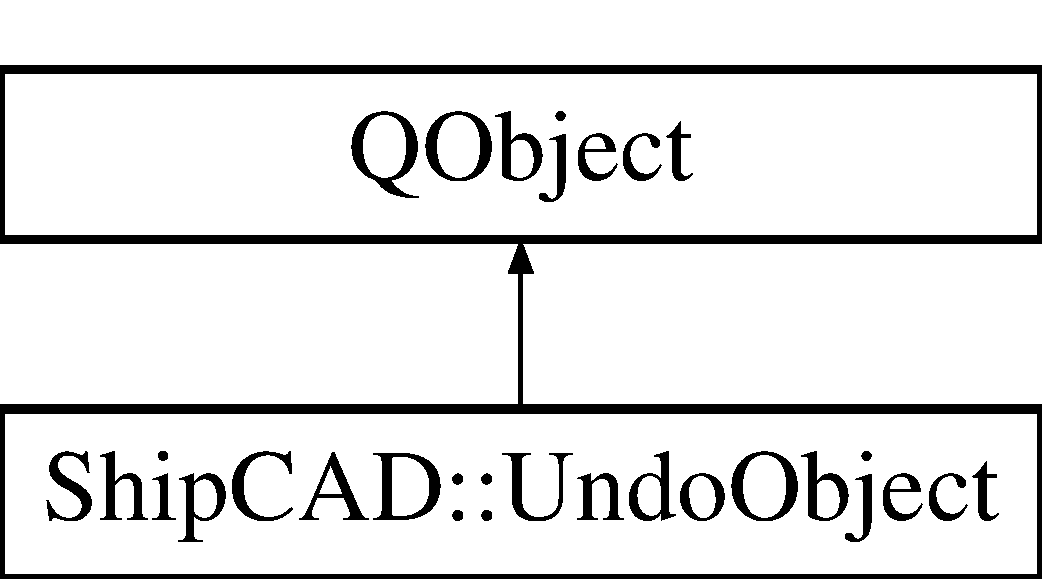
\includegraphics[height=2.000000cm]{classShipCAD_1_1UndoObject}
\end{center}
\end{figure}
\subsection*{Public Member Functions}
\begin{DoxyCompactItemize}
\item 
\hyperlink{classShipCAD_1_1UndoObject_a7822f20d55e4647ad4e4508b3e3f229b}{Undo\-Object} (\hyperlink{classShipCAD_1_1ShipCADModel}{Ship\-C\-A\-D\-Model} $\ast$owner, const Q\-String \&filename, \hyperlink{namespaceShipCAD_a66144e3f3a53da01f51c9bdb94fcae31}{edit\-\_\-mode\-\_\-t} mode, bool file\-\_\-changed, bool filename\-\_\-set, bool is\-\_\-temp\-\_\-redo\-\_\-ob)
\item 
\hyperlink{classShipCAD_1_1UndoObject_abfeebd1cd99df71bea798fafe15c474f}{$\sim$\-Undo\-Object} ()
\item 
size\-\_\-t \hyperlink{classShipCAD_1_1UndoObject_a74cc90d84599a153a37e13ab35018ff6}{get\-Memory} ()
\item 
bool \hyperlink{classShipCAD_1_1UndoObject_a9f949591bc4031ed4af67ce493e42d2e}{is\-Temp\-Redo\-Obj} ()
\item 
void \hyperlink{classShipCAD_1_1UndoObject_aecb1ca66c7c37fa2e1ef4ef2894bc9a4}{set\-Is\-Temp\-Redo\-Object} (bool set)
\item 
Q\-String \hyperlink{classShipCAD_1_1UndoObject_a6d71ab49eb2b14834a0263a4292fb851}{get\-Time} ()
\item 
Q\-String \& \hyperlink{classShipCAD_1_1UndoObject_abc895eabc12ece513bd763551f505a2e}{get\-Undo\-Text} ()
\item 
\hyperlink{classShipCAD_1_1FileBuffer}{File\-Buffer} \& \hyperlink{classShipCAD_1_1UndoObject_a160e77df4c6ae2bdefc5257aa8e6d85b}{get\-Undo\-Data} ()
\item 
void \hyperlink{classShipCAD_1_1UndoObject_a93bad349f284a0ff1cece56aa931f9e3}{accept} ()
\item 
void \hyperlink{classShipCAD_1_1UndoObject_a9cace556c2092492f681654d72e35ba6}{restore} ()
\end{DoxyCompactItemize}


\subsection{Detailed Description}


Definition at line 44 of file undoobject.\-h.



\subsection{Constructor \& Destructor Documentation}
\hypertarget{classShipCAD_1_1UndoObject_a7822f20d55e4647ad4e4508b3e3f229b}{\index{Ship\-C\-A\-D\-::\-Undo\-Object@{Ship\-C\-A\-D\-::\-Undo\-Object}!Undo\-Object@{Undo\-Object}}
\index{Undo\-Object@{Undo\-Object}!ShipCAD::UndoObject@{Ship\-C\-A\-D\-::\-Undo\-Object}}
\subsubsection[{Undo\-Object}]{\setlength{\rightskip}{0pt plus 5cm}Undo\-Object\-::\-Undo\-Object (
\begin{DoxyParamCaption}
\item[{{\bf Ship\-C\-A\-D\-Model} $\ast$}]{owner, }
\item[{const Q\-String \&}]{filename, }
\item[{{\bf edit\-\_\-mode\-\_\-t}}]{mode, }
\item[{bool}]{file\-\_\-changed, }
\item[{bool}]{filename\-\_\-set, }
\item[{bool}]{is\-\_\-temp\-\_\-redo\-\_\-ob}
\end{DoxyParamCaption}
)\hspace{0.3cm}{\ttfamily [explicit]}}}\label{classShipCAD_1_1UndoObject_a7822f20d55e4647ad4e4508b3e3f229b}


Definition at line 36 of file undoobject.\-cpp.

\hypertarget{classShipCAD_1_1UndoObject_abfeebd1cd99df71bea798fafe15c474f}{\index{Ship\-C\-A\-D\-::\-Undo\-Object@{Ship\-C\-A\-D\-::\-Undo\-Object}!$\sim$\-Undo\-Object@{$\sim$\-Undo\-Object}}
\index{$\sim$\-Undo\-Object@{$\sim$\-Undo\-Object}!ShipCAD::UndoObject@{Ship\-C\-A\-D\-::\-Undo\-Object}}
\subsubsection[{$\sim$\-Undo\-Object}]{\setlength{\rightskip}{0pt plus 5cm}Ship\-C\-A\-D\-::\-Undo\-Object\-::$\sim$\-Undo\-Object (
\begin{DoxyParamCaption}
{}
\end{DoxyParamCaption}
)\hspace{0.3cm}{\ttfamily [inline]}}}\label{classShipCAD_1_1UndoObject_abfeebd1cd99df71bea798fafe15c474f}


Definition at line 52 of file undoobject.\-h.



\subsection{Member Function Documentation}
\hypertarget{classShipCAD_1_1UndoObject_a93bad349f284a0ff1cece56aa931f9e3}{\index{Ship\-C\-A\-D\-::\-Undo\-Object@{Ship\-C\-A\-D\-::\-Undo\-Object}!accept@{accept}}
\index{accept@{accept}!ShipCAD::UndoObject@{Ship\-C\-A\-D\-::\-Undo\-Object}}
\subsubsection[{accept}]{\setlength{\rightskip}{0pt plus 5cm}void Undo\-Object\-::accept (
\begin{DoxyParamCaption}
{}
\end{DoxyParamCaption}
)}}\label{classShipCAD_1_1UndoObject_a93bad349f284a0ff1cece56aa931f9e3}


Definition at line 52 of file undoobject.\-cpp.

\hypertarget{classShipCAD_1_1UndoObject_a74cc90d84599a153a37e13ab35018ff6}{\index{Ship\-C\-A\-D\-::\-Undo\-Object@{Ship\-C\-A\-D\-::\-Undo\-Object}!get\-Memory@{get\-Memory}}
\index{get\-Memory@{get\-Memory}!ShipCAD::UndoObject@{Ship\-C\-A\-D\-::\-Undo\-Object}}
\subsubsection[{get\-Memory}]{\setlength{\rightskip}{0pt plus 5cm}size\-\_\-t Undo\-Object\-::get\-Memory (
\begin{DoxyParamCaption}
{}
\end{DoxyParamCaption}
)}}\label{classShipCAD_1_1UndoObject_a74cc90d84599a153a37e13ab35018ff6}


Definition at line 46 of file undoobject.\-cpp.

\hypertarget{classShipCAD_1_1UndoObject_a6d71ab49eb2b14834a0263a4292fb851}{\index{Ship\-C\-A\-D\-::\-Undo\-Object@{Ship\-C\-A\-D\-::\-Undo\-Object}!get\-Time@{get\-Time}}
\index{get\-Time@{get\-Time}!ShipCAD::UndoObject@{Ship\-C\-A\-D\-::\-Undo\-Object}}
\subsubsection[{get\-Time}]{\setlength{\rightskip}{0pt plus 5cm}Q\-String Ship\-C\-A\-D\-::\-Undo\-Object\-::get\-Time (
\begin{DoxyParamCaption}
{}
\end{DoxyParamCaption}
)\hspace{0.3cm}{\ttfamily [inline]}}}\label{classShipCAD_1_1UndoObject_a6d71ab49eb2b14834a0263a4292fb851}


Definition at line 59 of file undoobject.\-h.

\hypertarget{classShipCAD_1_1UndoObject_a160e77df4c6ae2bdefc5257aa8e6d85b}{\index{Ship\-C\-A\-D\-::\-Undo\-Object@{Ship\-C\-A\-D\-::\-Undo\-Object}!get\-Undo\-Data@{get\-Undo\-Data}}
\index{get\-Undo\-Data@{get\-Undo\-Data}!ShipCAD::UndoObject@{Ship\-C\-A\-D\-::\-Undo\-Object}}
\subsubsection[{get\-Undo\-Data}]{\setlength{\rightskip}{0pt plus 5cm}{\bf File\-Buffer}\& Ship\-C\-A\-D\-::\-Undo\-Object\-::get\-Undo\-Data (
\begin{DoxyParamCaption}
{}
\end{DoxyParamCaption}
)\hspace{0.3cm}{\ttfamily [inline]}}}\label{classShipCAD_1_1UndoObject_a160e77df4c6ae2bdefc5257aa8e6d85b}


Definition at line 63 of file undoobject.\-h.

\hypertarget{classShipCAD_1_1UndoObject_abc895eabc12ece513bd763551f505a2e}{\index{Ship\-C\-A\-D\-::\-Undo\-Object@{Ship\-C\-A\-D\-::\-Undo\-Object}!get\-Undo\-Text@{get\-Undo\-Text}}
\index{get\-Undo\-Text@{get\-Undo\-Text}!ShipCAD::UndoObject@{Ship\-C\-A\-D\-::\-Undo\-Object}}
\subsubsection[{get\-Undo\-Text}]{\setlength{\rightskip}{0pt plus 5cm}Q\-String\& Ship\-C\-A\-D\-::\-Undo\-Object\-::get\-Undo\-Text (
\begin{DoxyParamCaption}
{}
\end{DoxyParamCaption}
)\hspace{0.3cm}{\ttfamily [inline]}}}\label{classShipCAD_1_1UndoObject_abc895eabc12ece513bd763551f505a2e}


Definition at line 61 of file undoobject.\-h.

\hypertarget{classShipCAD_1_1UndoObject_a9f949591bc4031ed4af67ce493e42d2e}{\index{Ship\-C\-A\-D\-::\-Undo\-Object@{Ship\-C\-A\-D\-::\-Undo\-Object}!is\-Temp\-Redo\-Obj@{is\-Temp\-Redo\-Obj}}
\index{is\-Temp\-Redo\-Obj@{is\-Temp\-Redo\-Obj}!ShipCAD::UndoObject@{Ship\-C\-A\-D\-::\-Undo\-Object}}
\subsubsection[{is\-Temp\-Redo\-Obj}]{\setlength{\rightskip}{0pt plus 5cm}bool Ship\-C\-A\-D\-::\-Undo\-Object\-::is\-Temp\-Redo\-Obj (
\begin{DoxyParamCaption}
{}
\end{DoxyParamCaption}
)\hspace{0.3cm}{\ttfamily [inline]}}}\label{classShipCAD_1_1UndoObject_a9f949591bc4031ed4af67ce493e42d2e}


Definition at line 55 of file undoobject.\-h.

\hypertarget{classShipCAD_1_1UndoObject_a9cace556c2092492f681654d72e35ba6}{\index{Ship\-C\-A\-D\-::\-Undo\-Object@{Ship\-C\-A\-D\-::\-Undo\-Object}!restore@{restore}}
\index{restore@{restore}!ShipCAD::UndoObject@{Ship\-C\-A\-D\-::\-Undo\-Object}}
\subsubsection[{restore}]{\setlength{\rightskip}{0pt plus 5cm}void Undo\-Object\-::restore (
\begin{DoxyParamCaption}
{}
\end{DoxyParamCaption}
)}}\label{classShipCAD_1_1UndoObject_a9cace556c2092492f681654d72e35ba6}


Definition at line 81 of file undoobject.\-cpp.

\hypertarget{classShipCAD_1_1UndoObject_aecb1ca66c7c37fa2e1ef4ef2894bc9a4}{\index{Ship\-C\-A\-D\-::\-Undo\-Object@{Ship\-C\-A\-D\-::\-Undo\-Object}!set\-Is\-Temp\-Redo\-Object@{set\-Is\-Temp\-Redo\-Object}}
\index{set\-Is\-Temp\-Redo\-Object@{set\-Is\-Temp\-Redo\-Object}!ShipCAD::UndoObject@{Ship\-C\-A\-D\-::\-Undo\-Object}}
\subsubsection[{set\-Is\-Temp\-Redo\-Object}]{\setlength{\rightskip}{0pt plus 5cm}void Ship\-C\-A\-D\-::\-Undo\-Object\-::set\-Is\-Temp\-Redo\-Object (
\begin{DoxyParamCaption}
\item[{bool}]{set}
\end{DoxyParamCaption}
)\hspace{0.3cm}{\ttfamily [inline]}}}\label{classShipCAD_1_1UndoObject_aecb1ca66c7c37fa2e1ef4ef2894bc9a4}


Definition at line 57 of file undoobject.\-h.



The documentation for this class was generated from the following files\-:\begin{DoxyCompactItemize}
\item 
Ship\-C\-A\-Dlib/\hyperlink{undoobject_8h}{undoobject.\-h}\item 
Ship\-C\-A\-Dlib/\hyperlink{undoobject_8cpp}{undoobject.\-cpp}\end{DoxyCompactItemize}

\hypertarget{classShipCAD_1_1Viewport}{\section{Ship\-C\-A\-D\-:\-:Viewport Class Reference}
\label{classShipCAD_1_1Viewport}\index{Ship\-C\-A\-D\-::\-Viewport@{Ship\-C\-A\-D\-::\-Viewport}}
}


{\ttfamily \#include $<$viewport.\-h$>$}

Inheritance diagram for Ship\-C\-A\-D\-:\-:Viewport\-:\begin{figure}[H]
\begin{center}
\leavevmode
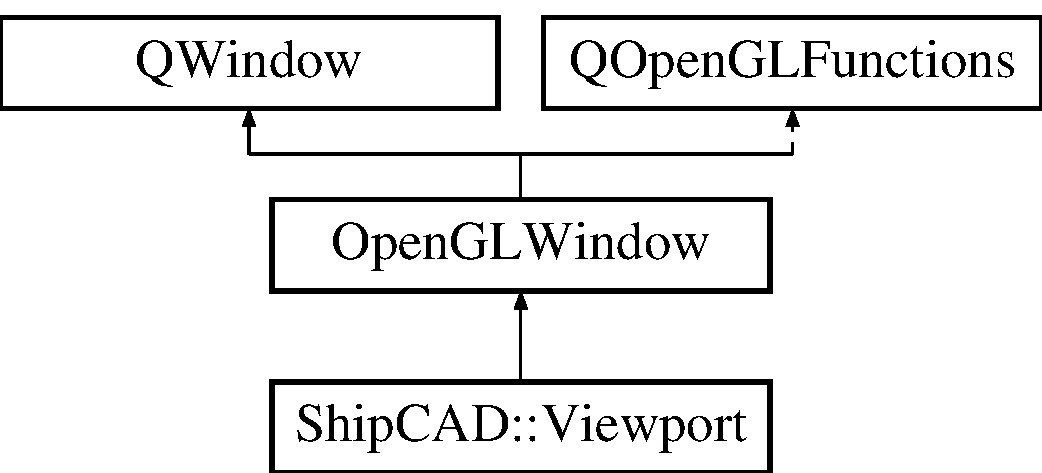
\includegraphics[height=3.000000cm]{classShipCAD_1_1Viewport}
\end{center}
\end{figure}
\subsection*{Public Slots}
\begin{DoxyCompactItemize}
\item 
void \hyperlink{classShipCAD_1_1Viewport_a578ac5ee96e36638739517fa21bf70c0}{set\-Viewport\-Mode} (\hyperlink{namespaceShipCAD_a67437198ee14f74e6c5277d761894863}{viewport\-\_\-mode\-\_\-t} mode)
\item 
void \hyperlink{classShipCAD_1_1Viewport_a554a3455c39ee5652b13c9b24c3c962e}{set\-Viewport\-Type} (\hyperlink{namespaceShipCAD_aeeeb05810f2e31ef89fd4ac6b6ba9c0a}{viewport\-\_\-type\-\_\-t} ty)
\item 
void \hyperlink{classShipCAD_1_1Viewport_a5f90a885e0204b32ff9795c4b79f824b}{set\-Camera\-Type} (\hyperlink{namespaceShipCAD_a58f51ebd2e66de5e41c2ffd6f434241e}{camera\-\_\-type\-\_\-t} val)
\item 
void \hyperlink{classShipCAD_1_1Viewport_a00ba2139fa06701b65de70d5c657f5d6}{set\-Angle} (float val)
\item 
void \hyperlink{classShipCAD_1_1Viewport_a4bda4b742dc477ed5dc2ab6ac7fe92bc}{set\-Elevation} (float val)
\item 
virtual void \hyperlink{classShipCAD_1_1Viewport_a4eeeb100fd88487215bb7794bdf5e0cb}{resize\-Event} (Q\-Resize\-Event $\ast$\hyperlink{classOpenGLWindow_a1e3045cffb900de55b7384f5091c9d94}{event})
\item 
bool \hyperlink{classShipCAD_1_1Viewport_ab247f28eb569e160142901b6eef265a3}{context\-Menu} (Q\-Mouse\-Event $\ast$\hyperlink{classOpenGLWindow_a1e3045cffb900de55b7384f5091c9d94}{event})
\end{DoxyCompactItemize}
\subsection*{Public Member Functions}
\begin{DoxyCompactItemize}
\item 
\hyperlink{classShipCAD_1_1Viewport_ad946e1cfc34e84610f9d89f3b62baf9d}{Viewport} (\hyperlink{classShipCAD_1_1Controller}{Controller} $\ast$ctl, \hyperlink{namespaceShipCAD_aeeeb05810f2e31ef89fd4ac6b6ba9c0a}{viewport\-\_\-type\-\_\-t} vtype)
\item 
\hyperlink{classShipCAD_1_1Viewport_a1e18a1ff4a52be33ef63d25034561850}{$\sim$\-Viewport} ()
\item 
void \hyperlink{classShipCAD_1_1Viewport_a9c35de3f7c9d7c860c494081b48309b3}{initialize} ()
\item 
void \hyperlink{classShipCAD_1_1Viewport_a9e81b526db3c2b508322c29b9fda5845}{render} ()
\item 
\hyperlink{classShipCAD_1_1Controller}{Controller} $\ast$ \hyperlink{classShipCAD_1_1Viewport_a4a12f9e56634caca61077572fe6b15f9}{get\-Controller} ()
\item 
\hyperlink{namespaceShipCAD_a67437198ee14f74e6c5277d761894863}{viewport\-\_\-mode\-\_\-t} \hyperlink{classShipCAD_1_1Viewport_a205e5082395c6d01660ffc179c57b83e}{get\-Viewport\-Mode} () const 
\item 
\hyperlink{namespaceShipCAD_aeeeb05810f2e31ef89fd4ac6b6ba9c0a}{viewport\-\_\-type\-\_\-t} \hyperlink{classShipCAD_1_1Viewport_a5f261a1925f09917013e8e532688326a}{get\-Viewport\-Type} () const 
\item 
void \hyperlink{classShipCAD_1_1Viewport_a886ac5965b63039799827da89bf3de20}{add\-Shader} (const std\-::string \&name, \hyperlink{classShipCAD_1_1Shader}{Shader} $\ast$shader)
\item 
\hyperlink{classShipCAD_1_1LineShader}{Line\-Shader} $\ast$ \hyperlink{classShipCAD_1_1Viewport_a0720a01f8650dc4acf89aad0649d9196}{set\-Line\-Shader} ()
\item 
\hyperlink{classShipCAD_1_1FaceShader}{Face\-Shader} $\ast$ \hyperlink{classShipCAD_1_1Viewport_ad6be617bdcab76cd2f44b0528371cd5d}{set\-Mono\-Face\-Shader} ()
\item 
\hyperlink{classShipCAD_1_1FaceShader}{Face\-Shader} $\ast$ \hyperlink{classShipCAD_1_1Viewport_a03cc2ed85178b9735c80b11dceb470b5}{set\-Lighted\-Face\-Shader} ()
\item 
bool \hyperlink{classShipCAD_1_1Viewport_aa9af80400534f46e5420916a2895ead5}{shoot\-Pick\-Ray} (\hyperlink{structShipCAD_1_1PickRay}{Pick\-Ray} \&ray)
\end{DoxyCompactItemize}
\subsection*{Protected Member Functions}
\begin{DoxyCompactItemize}
\item 
virtual void \hyperlink{classShipCAD_1_1Viewport_a7997e0e684a4f8b5709f4d98be6cebb4}{update} ()
\item 
virtual void \hyperlink{classShipCAD_1_1Viewport_a0dddc5b05c7308f8818a726b16a7d9eb}{mouse\-Press\-Event} (Q\-Mouse\-Event $\ast$)
\item 
virtual void \hyperlink{classShipCAD_1_1Viewport_a7cb6994a92d40990b58be272953b9120}{mouse\-Release\-Event} (Q\-Mouse\-Event $\ast$)
\item 
virtual void \hyperlink{classShipCAD_1_1Viewport_ab98dde7bb1d923b8cfc9a0c3cb249c2c}{mouse\-Move\-Event} (Q\-Mouse\-Event $\ast$)
\item 
virtual void \hyperlink{classShipCAD_1_1Viewport_a9ac4c18fa3454cddc5e73322c3d1afd8}{wheel\-Event} (Q\-Wheel\-Event $\ast$)
\item 
virtual void \hyperlink{classShipCAD_1_1Viewport_acc401d8a0d84810a9d695e3621e29b4e}{key\-Press\-Event} (Q\-Key\-Event $\ast$)
\end{DoxyCompactItemize}


\subsection{Detailed Description}


Definition at line 52 of file viewport.\-h.



\subsection{Constructor \& Destructor Documentation}
\hypertarget{classShipCAD_1_1Viewport_ad946e1cfc34e84610f9d89f3b62baf9d}{\index{Ship\-C\-A\-D\-::\-Viewport@{Ship\-C\-A\-D\-::\-Viewport}!Viewport@{Viewport}}
\index{Viewport@{Viewport}!ShipCAD::Viewport@{Ship\-C\-A\-D\-::\-Viewport}}
\subsubsection[{Viewport}]{\setlength{\rightskip}{0pt plus 5cm}Viewport\-::\-Viewport (
\begin{DoxyParamCaption}
\item[{{\bf Controller} $\ast$}]{ctl, }
\item[{{\bf viewport\-\_\-type\-\_\-t}}]{vtype}
\end{DoxyParamCaption}
)\hspace{0.3cm}{\ttfamily [explicit]}}}\label{classShipCAD_1_1Viewport_ad946e1cfc34e84610f9d89f3b62baf9d}


Definition at line 45 of file viewport.\-cpp.

\hypertarget{classShipCAD_1_1Viewport_a1e18a1ff4a52be33ef63d25034561850}{\index{Ship\-C\-A\-D\-::\-Viewport@{Ship\-C\-A\-D\-::\-Viewport}!$\sim$\-Viewport@{$\sim$\-Viewport}}
\index{$\sim$\-Viewport@{$\sim$\-Viewport}!ShipCAD::Viewport@{Ship\-C\-A\-D\-::\-Viewport}}
\subsubsection[{$\sim$\-Viewport}]{\setlength{\rightskip}{0pt plus 5cm}Viewport\-::$\sim$\-Viewport (
\begin{DoxyParamCaption}
{}
\end{DoxyParamCaption}
)}}\label{classShipCAD_1_1Viewport_a1e18a1ff4a52be33ef63d25034561850}


Definition at line 52 of file viewport.\-cpp.



\subsection{Member Function Documentation}
\hypertarget{classShipCAD_1_1Viewport_a886ac5965b63039799827da89bf3de20}{\index{Ship\-C\-A\-D\-::\-Viewport@{Ship\-C\-A\-D\-::\-Viewport}!add\-Shader@{add\-Shader}}
\index{add\-Shader@{add\-Shader}!ShipCAD::Viewport@{Ship\-C\-A\-D\-::\-Viewport}}
\subsubsection[{add\-Shader}]{\setlength{\rightskip}{0pt plus 5cm}void Viewport\-::add\-Shader (
\begin{DoxyParamCaption}
\item[{const std\-::string \&}]{name, }
\item[{{\bf Shader} $\ast$}]{shader}
\end{DoxyParamCaption}
)}}\label{classShipCAD_1_1Viewport_a886ac5965b63039799827da89bf3de20}


Definition at line 133 of file viewport.\-cpp.

\hypertarget{classShipCAD_1_1Viewport_ab247f28eb569e160142901b6eef265a3}{\index{Ship\-C\-A\-D\-::\-Viewport@{Ship\-C\-A\-D\-::\-Viewport}!context\-Menu@{context\-Menu}}
\index{context\-Menu@{context\-Menu}!ShipCAD::Viewport@{Ship\-C\-A\-D\-::\-Viewport}}
\subsubsection[{context\-Menu}]{\setlength{\rightskip}{0pt plus 5cm}bool Viewport\-::context\-Menu (
\begin{DoxyParamCaption}
\item[{Q\-Mouse\-Event $\ast$}]{event}
\end{DoxyParamCaption}
)\hspace{0.3cm}{\ttfamily [slot]}}}\label{classShipCAD_1_1Viewport_ab247f28eb569e160142901b6eef265a3}


Definition at line 209 of file viewport.\-cpp.

\hypertarget{classShipCAD_1_1Viewport_a4a12f9e56634caca61077572fe6b15f9}{\index{Ship\-C\-A\-D\-::\-Viewport@{Ship\-C\-A\-D\-::\-Viewport}!get\-Controller@{get\-Controller}}
\index{get\-Controller@{get\-Controller}!ShipCAD::Viewport@{Ship\-C\-A\-D\-::\-Viewport}}
\subsubsection[{get\-Controller}]{\setlength{\rightskip}{0pt plus 5cm}{\bf Controller}$\ast$ Ship\-C\-A\-D\-::\-Viewport\-::get\-Controller (
\begin{DoxyParamCaption}
{}
\end{DoxyParamCaption}
)\hspace{0.3cm}{\ttfamily [inline]}}}\label{classShipCAD_1_1Viewport_a4a12f9e56634caca61077572fe6b15f9}


Definition at line 63 of file viewport.\-h.

\hypertarget{classShipCAD_1_1Viewport_a205e5082395c6d01660ffc179c57b83e}{\index{Ship\-C\-A\-D\-::\-Viewport@{Ship\-C\-A\-D\-::\-Viewport}!get\-Viewport\-Mode@{get\-Viewport\-Mode}}
\index{get\-Viewport\-Mode@{get\-Viewport\-Mode}!ShipCAD::Viewport@{Ship\-C\-A\-D\-::\-Viewport}}
\subsubsection[{get\-Viewport\-Mode}]{\setlength{\rightskip}{0pt plus 5cm}{\bf viewport\-\_\-mode\-\_\-t} Ship\-C\-A\-D\-::\-Viewport\-::get\-Viewport\-Mode (
\begin{DoxyParamCaption}
{}
\end{DoxyParamCaption}
) const\hspace{0.3cm}{\ttfamily [inline]}}}\label{classShipCAD_1_1Viewport_a205e5082395c6d01660ffc179c57b83e}


Definition at line 65 of file viewport.\-h.

\hypertarget{classShipCAD_1_1Viewport_a5f261a1925f09917013e8e532688326a}{\index{Ship\-C\-A\-D\-::\-Viewport@{Ship\-C\-A\-D\-::\-Viewport}!get\-Viewport\-Type@{get\-Viewport\-Type}}
\index{get\-Viewport\-Type@{get\-Viewport\-Type}!ShipCAD::Viewport@{Ship\-C\-A\-D\-::\-Viewport}}
\subsubsection[{get\-Viewport\-Type}]{\setlength{\rightskip}{0pt plus 5cm}{\bf viewport\-\_\-type\-\_\-t} Ship\-C\-A\-D\-::\-Viewport\-::get\-Viewport\-Type (
\begin{DoxyParamCaption}
{}
\end{DoxyParamCaption}
) const\hspace{0.3cm}{\ttfamily [inline]}}}\label{classShipCAD_1_1Viewport_a5f261a1925f09917013e8e532688326a}


Definition at line 67 of file viewport.\-h.

\hypertarget{classShipCAD_1_1Viewport_a9c35de3f7c9d7c860c494081b48309b3}{\index{Ship\-C\-A\-D\-::\-Viewport@{Ship\-C\-A\-D\-::\-Viewport}!initialize@{initialize}}
\index{initialize@{initialize}!ShipCAD::Viewport@{Ship\-C\-A\-D\-::\-Viewport}}
\subsubsection[{initialize}]{\setlength{\rightskip}{0pt plus 5cm}void Viewport\-::initialize (
\begin{DoxyParamCaption}
{}
\end{DoxyParamCaption}
)\hspace{0.3cm}{\ttfamily [virtual]}}}\label{classShipCAD_1_1Viewport_a9c35de3f7c9d7c860c494081b48309b3}


Reimplemented from \hyperlink{classOpenGLWindow_aed4e2ee22e113b2f7e7d1eba4ef1b965}{Open\-G\-L\-Window}.



Definition at line 63 of file viewport.\-cpp.

\hypertarget{classShipCAD_1_1Viewport_acc401d8a0d84810a9d695e3621e29b4e}{\index{Ship\-C\-A\-D\-::\-Viewport@{Ship\-C\-A\-D\-::\-Viewport}!key\-Press\-Event@{key\-Press\-Event}}
\index{key\-Press\-Event@{key\-Press\-Event}!ShipCAD::Viewport@{Ship\-C\-A\-D\-::\-Viewport}}
\subsubsection[{key\-Press\-Event}]{\setlength{\rightskip}{0pt plus 5cm}void Viewport\-::key\-Press\-Event (
\begin{DoxyParamCaption}
\item[{Q\-Key\-Event $\ast$}]{event}
\end{DoxyParamCaption}
)\hspace{0.3cm}{\ttfamily [protected]}, {\ttfamily [virtual]}}}\label{classShipCAD_1_1Viewport_acc401d8a0d84810a9d695e3621e29b4e}


Definition at line 302 of file viewport.\-cpp.

\hypertarget{classShipCAD_1_1Viewport_ab98dde7bb1d923b8cfc9a0c3cb249c2c}{\index{Ship\-C\-A\-D\-::\-Viewport@{Ship\-C\-A\-D\-::\-Viewport}!mouse\-Move\-Event@{mouse\-Move\-Event}}
\index{mouse\-Move\-Event@{mouse\-Move\-Event}!ShipCAD::Viewport@{Ship\-C\-A\-D\-::\-Viewport}}
\subsubsection[{mouse\-Move\-Event}]{\setlength{\rightskip}{0pt plus 5cm}void Viewport\-::mouse\-Move\-Event (
\begin{DoxyParamCaption}
\item[{Q\-Mouse\-Event $\ast$}]{event}
\end{DoxyParamCaption}
)\hspace{0.3cm}{\ttfamily [protected]}, {\ttfamily [virtual]}}}\label{classShipCAD_1_1Viewport_ab98dde7bb1d923b8cfc9a0c3cb249c2c}


Definition at line 256 of file viewport.\-cpp.

\hypertarget{classShipCAD_1_1Viewport_a0dddc5b05c7308f8818a726b16a7d9eb}{\index{Ship\-C\-A\-D\-::\-Viewport@{Ship\-C\-A\-D\-::\-Viewport}!mouse\-Press\-Event@{mouse\-Press\-Event}}
\index{mouse\-Press\-Event@{mouse\-Press\-Event}!ShipCAD::Viewport@{Ship\-C\-A\-D\-::\-Viewport}}
\subsubsection[{mouse\-Press\-Event}]{\setlength{\rightskip}{0pt plus 5cm}void Viewport\-::mouse\-Press\-Event (
\begin{DoxyParamCaption}
\item[{Q\-Mouse\-Event $\ast$}]{event}
\end{DoxyParamCaption}
)\hspace{0.3cm}{\ttfamily [protected]}, {\ttfamily [virtual]}}}\label{classShipCAD_1_1Viewport_a0dddc5b05c7308f8818a726b16a7d9eb}


Definition at line 219 of file viewport.\-cpp.

\hypertarget{classShipCAD_1_1Viewport_a7cb6994a92d40990b58be272953b9120}{\index{Ship\-C\-A\-D\-::\-Viewport@{Ship\-C\-A\-D\-::\-Viewport}!mouse\-Release\-Event@{mouse\-Release\-Event}}
\index{mouse\-Release\-Event@{mouse\-Release\-Event}!ShipCAD::Viewport@{Ship\-C\-A\-D\-::\-Viewport}}
\subsubsection[{mouse\-Release\-Event}]{\setlength{\rightskip}{0pt plus 5cm}void Viewport\-::mouse\-Release\-Event (
\begin{DoxyParamCaption}
\item[{Q\-Mouse\-Event $\ast$}]{event}
\end{DoxyParamCaption}
)\hspace{0.3cm}{\ttfamily [protected]}, {\ttfamily [virtual]}}}\label{classShipCAD_1_1Viewport_a7cb6994a92d40990b58be272953b9120}


Definition at line 230 of file viewport.\-cpp.

\hypertarget{classShipCAD_1_1Viewport_a9e81b526db3c2b508322c29b9fda5845}{\index{Ship\-C\-A\-D\-::\-Viewport@{Ship\-C\-A\-D\-::\-Viewport}!render@{render}}
\index{render@{render}!ShipCAD::Viewport@{Ship\-C\-A\-D\-::\-Viewport}}
\subsubsection[{render}]{\setlength{\rightskip}{0pt plus 5cm}void Viewport\-::render (
\begin{DoxyParamCaption}
{}
\end{DoxyParamCaption}
)\hspace{0.3cm}{\ttfamily [virtual]}}}\label{classShipCAD_1_1Viewport_a9e81b526db3c2b508322c29b9fda5845}


Reimplemented from \hyperlink{classOpenGLWindow_ac9e094864803a0b29364f42c2a47fa8c}{Open\-G\-L\-Window}.



Definition at line 138 of file viewport.\-cpp.

\hypertarget{classShipCAD_1_1Viewport_a4eeeb100fd88487215bb7794bdf5e0cb}{\index{Ship\-C\-A\-D\-::\-Viewport@{Ship\-C\-A\-D\-::\-Viewport}!resize\-Event@{resize\-Event}}
\index{resize\-Event@{resize\-Event}!ShipCAD::Viewport@{Ship\-C\-A\-D\-::\-Viewport}}
\subsubsection[{resize\-Event}]{\setlength{\rightskip}{0pt plus 5cm}void Viewport\-::resize\-Event (
\begin{DoxyParamCaption}
\item[{Q\-Resize\-Event $\ast$}]{event}
\end{DoxyParamCaption}
)\hspace{0.3cm}{\ttfamily [virtual]}, {\ttfamily [slot]}}}\label{classShipCAD_1_1Viewport_a4eeeb100fd88487215bb7794bdf5e0cb}


Definition at line 118 of file viewport.\-cpp.

\hypertarget{classShipCAD_1_1Viewport_a00ba2139fa06701b65de70d5c657f5d6}{\index{Ship\-C\-A\-D\-::\-Viewport@{Ship\-C\-A\-D\-::\-Viewport}!set\-Angle@{set\-Angle}}
\index{set\-Angle@{set\-Angle}!ShipCAD::Viewport@{Ship\-C\-A\-D\-::\-Viewport}}
\subsubsection[{set\-Angle}]{\setlength{\rightskip}{0pt plus 5cm}void Viewport\-::set\-Angle (
\begin{DoxyParamCaption}
\item[{float}]{val}
\end{DoxyParamCaption}
)\hspace{0.3cm}{\ttfamily [slot]}}}\label{classShipCAD_1_1Viewport_a00ba2139fa06701b65de70d5c657f5d6}


Definition at line 100 of file viewport.\-cpp.

\hypertarget{classShipCAD_1_1Viewport_a5f90a885e0204b32ff9795c4b79f824b}{\index{Ship\-C\-A\-D\-::\-Viewport@{Ship\-C\-A\-D\-::\-Viewport}!set\-Camera\-Type@{set\-Camera\-Type}}
\index{set\-Camera\-Type@{set\-Camera\-Type}!ShipCAD::Viewport@{Ship\-C\-A\-D\-::\-Viewport}}
\subsubsection[{set\-Camera\-Type}]{\setlength{\rightskip}{0pt plus 5cm}void Viewport\-::set\-Camera\-Type (
\begin{DoxyParamCaption}
\item[{{\bf camera\-\_\-type\-\_\-t}}]{val}
\end{DoxyParamCaption}
)\hspace{0.3cm}{\ttfamily [slot]}}}\label{classShipCAD_1_1Viewport_a5f90a885e0204b32ff9795c4b79f824b}


Definition at line 81 of file viewport.\-cpp.

\hypertarget{classShipCAD_1_1Viewport_a4bda4b742dc477ed5dc2ab6ac7fe92bc}{\index{Ship\-C\-A\-D\-::\-Viewport@{Ship\-C\-A\-D\-::\-Viewport}!set\-Elevation@{set\-Elevation}}
\index{set\-Elevation@{set\-Elevation}!ShipCAD::Viewport@{Ship\-C\-A\-D\-::\-Viewport}}
\subsubsection[{set\-Elevation}]{\setlength{\rightskip}{0pt plus 5cm}void Viewport\-::set\-Elevation (
\begin{DoxyParamCaption}
\item[{float}]{val}
\end{DoxyParamCaption}
)\hspace{0.3cm}{\ttfamily [slot]}}}\label{classShipCAD_1_1Viewport_a4bda4b742dc477ed5dc2ab6ac7fe92bc}


Definition at line 109 of file viewport.\-cpp.

\hypertarget{classShipCAD_1_1Viewport_a03cc2ed85178b9735c80b11dceb470b5}{\index{Ship\-C\-A\-D\-::\-Viewport@{Ship\-C\-A\-D\-::\-Viewport}!set\-Lighted\-Face\-Shader@{set\-Lighted\-Face\-Shader}}
\index{set\-Lighted\-Face\-Shader@{set\-Lighted\-Face\-Shader}!ShipCAD::Viewport@{Ship\-C\-A\-D\-::\-Viewport}}
\subsubsection[{set\-Lighted\-Face\-Shader}]{\setlength{\rightskip}{0pt plus 5cm}{\bf Face\-Shader} $\ast$ Viewport\-::set\-Lighted\-Face\-Shader (
\begin{DoxyParamCaption}
{}
\end{DoxyParamCaption}
)}}\label{classShipCAD_1_1Viewport_a03cc2ed85178b9735c80b11dceb470b5}


Definition at line 195 of file viewport.\-cpp.

\hypertarget{classShipCAD_1_1Viewport_a0720a01f8650dc4acf89aad0649d9196}{\index{Ship\-C\-A\-D\-::\-Viewport@{Ship\-C\-A\-D\-::\-Viewport}!set\-Line\-Shader@{set\-Line\-Shader}}
\index{set\-Line\-Shader@{set\-Line\-Shader}!ShipCAD::Viewport@{Ship\-C\-A\-D\-::\-Viewport}}
\subsubsection[{set\-Line\-Shader}]{\setlength{\rightskip}{0pt plus 5cm}{\bf Line\-Shader} $\ast$ Viewport\-::set\-Line\-Shader (
\begin{DoxyParamCaption}
{}
\end{DoxyParamCaption}
)}}\label{classShipCAD_1_1Viewport_a0720a01f8650dc4acf89aad0649d9196}


Definition at line 167 of file viewport.\-cpp.

\hypertarget{classShipCAD_1_1Viewport_ad6be617bdcab76cd2f44b0528371cd5d}{\index{Ship\-C\-A\-D\-::\-Viewport@{Ship\-C\-A\-D\-::\-Viewport}!set\-Mono\-Face\-Shader@{set\-Mono\-Face\-Shader}}
\index{set\-Mono\-Face\-Shader@{set\-Mono\-Face\-Shader}!ShipCAD::Viewport@{Ship\-C\-A\-D\-::\-Viewport}}
\subsubsection[{set\-Mono\-Face\-Shader}]{\setlength{\rightskip}{0pt plus 5cm}{\bf Face\-Shader} $\ast$ Viewport\-::set\-Mono\-Face\-Shader (
\begin{DoxyParamCaption}
{}
\end{DoxyParamCaption}
)}}\label{classShipCAD_1_1Viewport_ad6be617bdcab76cd2f44b0528371cd5d}


Definition at line 181 of file viewport.\-cpp.

\hypertarget{classShipCAD_1_1Viewport_a578ac5ee96e36638739517fa21bf70c0}{\index{Ship\-C\-A\-D\-::\-Viewport@{Ship\-C\-A\-D\-::\-Viewport}!set\-Viewport\-Mode@{set\-Viewport\-Mode}}
\index{set\-Viewport\-Mode@{set\-Viewport\-Mode}!ShipCAD::Viewport@{Ship\-C\-A\-D\-::\-Viewport}}
\subsubsection[{set\-Viewport\-Mode}]{\setlength{\rightskip}{0pt plus 5cm}void Viewport\-::set\-Viewport\-Mode (
\begin{DoxyParamCaption}
\item[{{\bf viewport\-\_\-mode\-\_\-t}}]{mode}
\end{DoxyParamCaption}
)\hspace{0.3cm}{\ttfamily [slot]}}}\label{classShipCAD_1_1Viewport_a578ac5ee96e36638739517fa21bf70c0}


Definition at line 75 of file viewport.\-cpp.

\hypertarget{classShipCAD_1_1Viewport_a554a3455c39ee5652b13c9b24c3c962e}{\index{Ship\-C\-A\-D\-::\-Viewport@{Ship\-C\-A\-D\-::\-Viewport}!set\-Viewport\-Type@{set\-Viewport\-Type}}
\index{set\-Viewport\-Type@{set\-Viewport\-Type}!ShipCAD::Viewport@{Ship\-C\-A\-D\-::\-Viewport}}
\subsubsection[{set\-Viewport\-Type}]{\setlength{\rightskip}{0pt plus 5cm}void Viewport\-::set\-Viewport\-Type (
\begin{DoxyParamCaption}
\item[{{\bf viewport\-\_\-type\-\_\-t}}]{ty}
\end{DoxyParamCaption}
)\hspace{0.3cm}{\ttfamily [slot]}}}\label{classShipCAD_1_1Viewport_a554a3455c39ee5652b13c9b24c3c962e}


Definition at line 90 of file viewport.\-cpp.

\hypertarget{classShipCAD_1_1Viewport_aa9af80400534f46e5420916a2895ead5}{\index{Ship\-C\-A\-D\-::\-Viewport@{Ship\-C\-A\-D\-::\-Viewport}!shoot\-Pick\-Ray@{shoot\-Pick\-Ray}}
\index{shoot\-Pick\-Ray@{shoot\-Pick\-Ray}!ShipCAD::Viewport@{Ship\-C\-A\-D\-::\-Viewport}}
\subsubsection[{shoot\-Pick\-Ray}]{\setlength{\rightskip}{0pt plus 5cm}bool Viewport\-::shoot\-Pick\-Ray (
\begin{DoxyParamCaption}
\item[{{\bf Pick\-Ray} \&}]{ray}
\end{DoxyParamCaption}
)}}\label{classShipCAD_1_1Viewport_aa9af80400534f46e5420916a2895ead5}


Definition at line 310 of file viewport.\-cpp.

\hypertarget{classShipCAD_1_1Viewport_a7997e0e684a4f8b5709f4d98be6cebb4}{\index{Ship\-C\-A\-D\-::\-Viewport@{Ship\-C\-A\-D\-::\-Viewport}!update@{update}}
\index{update@{update}!ShipCAD::Viewport@{Ship\-C\-A\-D\-::\-Viewport}}
\subsubsection[{update}]{\setlength{\rightskip}{0pt plus 5cm}void Viewport\-::update (
\begin{DoxyParamCaption}
{}
\end{DoxyParamCaption}
)\hspace{0.3cm}{\ttfamily [protected]}, {\ttfamily [virtual]}}}\label{classShipCAD_1_1Viewport_a7997e0e684a4f8b5709f4d98be6cebb4}


Definition at line 125 of file viewport.\-cpp.

\hypertarget{classShipCAD_1_1Viewport_a9ac4c18fa3454cddc5e73322c3d1afd8}{\index{Ship\-C\-A\-D\-::\-Viewport@{Ship\-C\-A\-D\-::\-Viewport}!wheel\-Event@{wheel\-Event}}
\index{wheel\-Event@{wheel\-Event}!ShipCAD::Viewport@{Ship\-C\-A\-D\-::\-Viewport}}
\subsubsection[{wheel\-Event}]{\setlength{\rightskip}{0pt plus 5cm}void Viewport\-::wheel\-Event (
\begin{DoxyParamCaption}
\item[{Q\-Wheel\-Event $\ast$}]{event}
\end{DoxyParamCaption}
)\hspace{0.3cm}{\ttfamily [protected]}, {\ttfamily [virtual]}}}\label{classShipCAD_1_1Viewport_a9ac4c18fa3454cddc5e73322c3d1afd8}


Definition at line 285 of file viewport.\-cpp.



The documentation for this class was generated from the following files\-:\begin{DoxyCompactItemize}
\item 
Ship\-C\-A\-Dlib/\hyperlink{viewport_8h}{viewport.\-h}\item 
Ship\-C\-A\-Dlib/\hyperlink{viewport_8cpp}{viewport.\-cpp}\end{DoxyCompactItemize}

\hypertarget{classShipCAD_1_1Visibility}{\section{Ship\-C\-A\-D\-:\-:Visibility Class Reference}
\label{classShipCAD_1_1Visibility}\index{Ship\-C\-A\-D\-::\-Visibility@{Ship\-C\-A\-D\-::\-Visibility}}
}


Settings class for visibility of different features.  




{\ttfamily \#include $<$visibility.\-h$>$}

Inheritance diagram for Ship\-C\-A\-D\-:\-:Visibility\-:\begin{figure}[H]
\begin{center}
\leavevmode
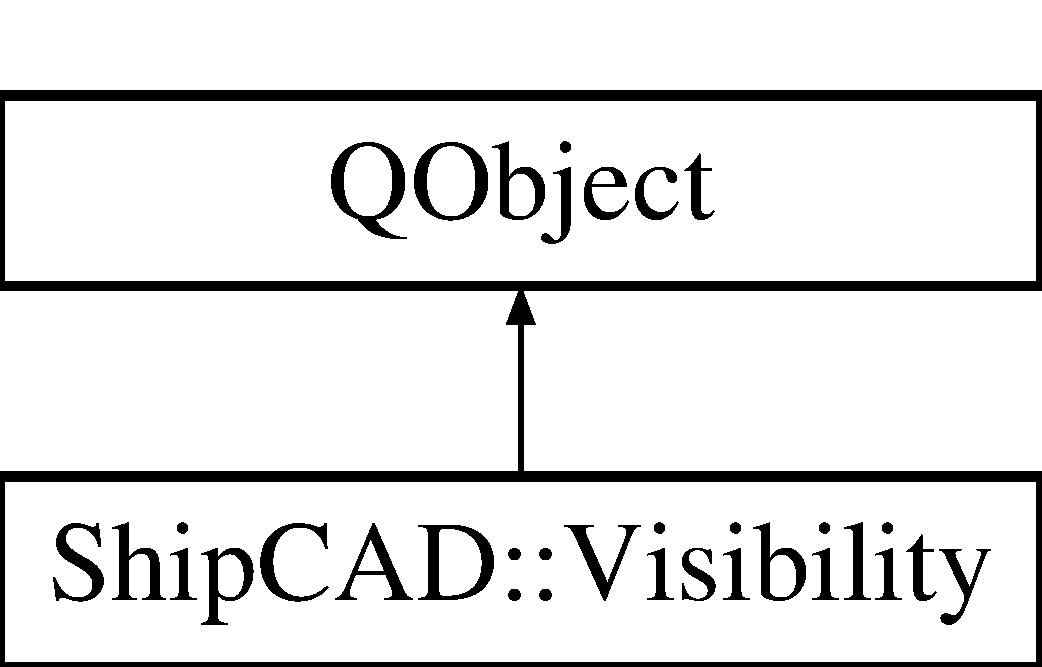
\includegraphics[height=2.000000cm]{classShipCAD_1_1Visibility}
\end{center}
\end{figure}
\subsection*{Public Slots}
\begin{DoxyCompactItemize}
\item 
void \hyperlink{classShipCAD_1_1Visibility_aa9ff89a0d825c2e5ac3fe9c08da9daec}{decrease\-Curvature\-Scale} ()
\item 
void \hyperlink{classShipCAD_1_1Visibility_af8ff6d1f77f64179f186a200ef7d056c}{increase\-Curvature\-Scale} ()
\end{DoxyCompactItemize}
\subsection*{Signals}
\begin{DoxyCompactItemize}
\item 
void \hyperlink{classShipCAD_1_1Visibility_a16de65dec1636dd1edc69b15d84c7735}{on\-Change\-Cursor\-Increment} ()
\end{DoxyCompactItemize}
\subsection*{Public Member Functions}
\begin{DoxyCompactItemize}
\item 
\hyperlink{classShipCAD_1_1Visibility_a7b3d38d4dd65392de8b2bac001afe6e8}{Visibility} (\hyperlink{classShipCAD_1_1ShipCADModel}{Ship\-C\-A\-D\-Model} $\ast$owner)
\begin{DoxyCompactList}\small\item\em constructor \end{DoxyCompactList}\item 
\hyperlink{classShipCAD_1_1Visibility_a653098c74de41abb0a46c455b24c9d3a}{$\sim$\-Visibility} ()
\begin{DoxyCompactList}\small\item\em destructor \end{DoxyCompactList}\item 
void \hyperlink{classShipCAD_1_1Visibility_a665efac6ef5dfdd3baab521fcbd96cb6}{set\-Cursor\-Increment} (float val)
\item 
float \hyperlink{classShipCAD_1_1Visibility_ae8cdc39bcc513f1bb66d0c39fdd1c46a}{get\-Curvature\-Scale} () const 
\begin{DoxyCompactList}\small\item\em get curvature scale \end{DoxyCompactList}\item 
void \hyperlink{classShipCAD_1_1Visibility_a5487027d259912f366351938a1a87085}{set\-Curvature\-Scale} (float val)
\begin{DoxyCompactList}\small\item\em set curvature scale \end{DoxyCompactList}\item 
bool \hyperlink{classShipCAD_1_1Visibility_a293f2a74bb76c65b7fa706e8aac353f1}{is\-Show\-Buttocks} () const 
\begin{DoxyCompactList}\small\item\em show visibility of buttocks \end{DoxyCompactList}\item 
void \hyperlink{classShipCAD_1_1Visibility_a8e7776fdc776e8fa96b7e9bce1cffdce}{set\-Show\-Buttocks} (bool show)
\begin{DoxyCompactList}\small\item\em set visibility of buttocks \end{DoxyCompactList}\item 
bool \hyperlink{classShipCAD_1_1Visibility_a177cc880657723c1cbcc4c66c16ee208}{is\-Show\-Control\-Net} () const 
\begin{DoxyCompactList}\small\item\em is control net shown \end{DoxyCompactList}\item 
void \hyperlink{classShipCAD_1_1Visibility_a7498435ee6955772713b113a63279260}{set\-Show\-Control\-Net} (bool show)
\begin{DoxyCompactList}\small\item\em set visibility of control net \end{DoxyCompactList}\item 
bool \hyperlink{classShipCAD_1_1Visibility_a36f2e03d75a5a2cfcfc3c637c08bee92}{is\-Show\-Curvature} () const 
\begin{DoxyCompactList}\small\item\em show visibility of curvature \end{DoxyCompactList}\item 
void \hyperlink{classShipCAD_1_1Visibility_a72fa3ed8c721fffe65b29c61329a1d35}{set\-Show\-Curvature} (bool show)
\begin{DoxyCompactList}\small\item\em set show curvature \end{DoxyCompactList}\item 
bool \hyperlink{classShipCAD_1_1Visibility_afa9ae51a7f178d93fe7d6b12ea5a4e63}{is\-Show\-Diagonals} () const 
\begin{DoxyCompactList}\small\item\em show visibility of diagonals \end{DoxyCompactList}\item 
void \hyperlink{classShipCAD_1_1Visibility_a02ff571862dacdbec3248a80ec42eb4f}{set\-Show\-Diagonals} (bool show)
\begin{DoxyCompactList}\small\item\em set show diagonals \end{DoxyCompactList}\item 
bool \hyperlink{classShipCAD_1_1Visibility_a39e12b36d20e2e3ad750e18c248a04f5}{is\-Show\-Flowlines} () const 
\begin{DoxyCompactList}\small\item\em show visibility of flowlines \end{DoxyCompactList}\item 
void \hyperlink{classShipCAD_1_1Visibility_a805b3f5f4a8d7c6b578a79c2539cf192}{set\-Show\-Flowlines} (bool show)
\begin{DoxyCompactList}\small\item\em set show flowlines \end{DoxyCompactList}\item 
bool \hyperlink{classShipCAD_1_1Visibility_a9aa81550e01813b9ec84b40aba5f904e}{is\-Show\-Grid} () const 
\begin{DoxyCompactList}\small\item\em is grid shown \end{DoxyCompactList}\item 
void \hyperlink{classShipCAD_1_1Visibility_a57b601879f10927beb3d466c211e6ee6}{set\-Show\-Grid} (bool show)
\begin{DoxyCompactList}\small\item\em set visibility of grid \end{DoxyCompactList}\item 
\hyperlink{namespaceShipCAD_a742f9cd95e62e207769e17467ecd5bb7}{model\-\_\-view\-\_\-t} \hyperlink{classShipCAD_1_1Visibility_a34d56f9e9467b9749c6b50adfe8a0493}{get\-Model\-View} () const 
\begin{DoxyCompactList}\small\item\em get model view setting \end{DoxyCompactList}\item 
void \hyperlink{classShipCAD_1_1Visibility_a017115fc25ec3a7363033dcca873f38f}{set\-Model\-View} (\hyperlink{namespaceShipCAD_a742f9cd95e62e207769e17467ecd5bb7}{model\-\_\-view\-\_\-t} vw)
\begin{DoxyCompactList}\small\item\em set model view \end{DoxyCompactList}\item 
bool \hyperlink{classShipCAD_1_1Visibility_a63588a3b8aa0a7dd37b19173a4802b47}{is\-Show\-Interior\-Edges} () const 
\begin{DoxyCompactList}\small\item\em is interior edges shown \end{DoxyCompactList}\item 
void \hyperlink{classShipCAD_1_1Visibility_a2ce6cd0c56750e6638b5e195e6bc5590}{set\-Show\-Interior\-Edges} (bool show)
\begin{DoxyCompactList}\small\item\em set visibility of interior edges \end{DoxyCompactList}\item 
bool \hyperlink{classShipCAD_1_1Visibility_adae35f2eb31f5d468674ab9856a39637}{is\-Show\-Markers} () const 
\begin{DoxyCompactList}\small\item\em show visibility of markers \end{DoxyCompactList}\item 
void \hyperlink{classShipCAD_1_1Visibility_a04cd6f732b4334070aef1f43b457d472}{set\-Show\-Markers} (bool show)
\begin{DoxyCompactList}\small\item\em set visiblity of markers \end{DoxyCompactList}\item 
bool \hyperlink{classShipCAD_1_1Visibility_a973f63d7828898c1499607a8d87b430d}{is\-Show\-Normals} () const 
\begin{DoxyCompactList}\small\item\em show visibility of normals \end{DoxyCompactList}\item 
void \hyperlink{classShipCAD_1_1Visibility_a78971bef725cdc53fa600589d68b628a}{set\-Show\-Normals} (bool show)
\begin{DoxyCompactList}\small\item\em set visibility of normals \end{DoxyCompactList}\item 
bool \hyperlink{classShipCAD_1_1Visibility_a02ae626d57305729ff870e14dd7f6e26}{is\-Show\-Stations} () const 
\begin{DoxyCompactList}\small\item\em show visibility of stations \end{DoxyCompactList}\item 
void \hyperlink{classShipCAD_1_1Visibility_a41a2754fcdbe69609b837fc9be26135e}{set\-Show\-Stations} (bool show)
\begin{DoxyCompactList}\small\item\em set visibility of stations \end{DoxyCompactList}\item 
bool \hyperlink{classShipCAD_1_1Visibility_a5ada95979a3d66b792b394f7c065b1fd}{is\-Show\-Waterlines} () const 
\begin{DoxyCompactList}\small\item\em show visiblity of waterlines \end{DoxyCompactList}\item 
void \hyperlink{classShipCAD_1_1Visibility_ac07b5944afd8a44c569aef09ee893450}{set\-Show\-Waterlines} (bool show)
\begin{DoxyCompactList}\small\item\em set visibility of waterlines \end{DoxyCompactList}\item 
bool \hyperlink{classShipCAD_1_1Visibility_adf96eb2133086a34056f6c0f75556f13}{is\-Show\-Control\-Curves} () const 
\begin{DoxyCompactList}\small\item\em show visibility of control curves \end{DoxyCompactList}\item 
void \hyperlink{classShipCAD_1_1Visibility_a760ef76f6db721925ee95cefaae966de}{set\-Show\-Control\-Curves} (bool show)
\begin{DoxyCompactList}\small\item\em set visibility of control curves \end{DoxyCompactList}\item 
bool \hyperlink{classShipCAD_1_1Visibility_a48ceac6b27669e53b197179e81c00126}{is\-Show\-Hydro\-Data} () const 
\begin{DoxyCompactList}\small\item\em show visibility of hydrostatic data \end{DoxyCompactList}\item 
void \hyperlink{classShipCAD_1_1Visibility_afc3530bd2d3fc1e71fa699aace76e4ea}{set\-Show\-Hydro\-Data} (bool show)
\begin{DoxyCompactList}\small\item\em set visibility of Hydrostatic data \end{DoxyCompactList}\item 
void \hyperlink{classShipCAD_1_1Visibility_a418d8fcee4c8f7c0c5c0691249ded677}{load\-Binary} (\hyperlink{classShipCAD_1_1FileBuffer}{File\-Buffer} \&source)
\item 
void \hyperlink{classShipCAD_1_1Visibility_adaf76df822f6f03a93a1b827c81fe58f}{save\-Binary} (\hyperlink{classShipCAD_1_1FileBuffer}{File\-Buffer} \&dest)
\item 
void \hyperlink{classShipCAD_1_1Visibility_af3e925196f71caa8e8ddabd2e7210bbf}{clear} ()
\end{DoxyCompactItemize}


\subsection{Detailed Description}
Settings class for visibility of different features. 

Definition at line 48 of file visibility.\-h.



\subsection{Constructor \& Destructor Documentation}
\hypertarget{classShipCAD_1_1Visibility_a7b3d38d4dd65392de8b2bac001afe6e8}{\index{Ship\-C\-A\-D\-::\-Visibility@{Ship\-C\-A\-D\-::\-Visibility}!Visibility@{Visibility}}
\index{Visibility@{Visibility}!ShipCAD::Visibility@{Ship\-C\-A\-D\-::\-Visibility}}
\subsubsection[{Visibility}]{\setlength{\rightskip}{0pt plus 5cm}Visibility\-::\-Visibility (
\begin{DoxyParamCaption}
\item[{{\bf Ship\-C\-A\-D\-Model} $\ast$}]{owner}
\end{DoxyParamCaption}
)\hspace{0.3cm}{\ttfamily [explicit]}}}\label{classShipCAD_1_1Visibility_a7b3d38d4dd65392de8b2bac001afe6e8}


constructor 



Definition at line 36 of file visibility.\-cpp.

\hypertarget{classShipCAD_1_1Visibility_a653098c74de41abb0a46c455b24c9d3a}{\index{Ship\-C\-A\-D\-::\-Visibility@{Ship\-C\-A\-D\-::\-Visibility}!$\sim$\-Visibility@{$\sim$\-Visibility}}
\index{$\sim$\-Visibility@{$\sim$\-Visibility}!ShipCAD::Visibility@{Ship\-C\-A\-D\-::\-Visibility}}
\subsubsection[{$\sim$\-Visibility}]{\setlength{\rightskip}{0pt plus 5cm}Ship\-C\-A\-D\-::\-Visibility\-::$\sim$\-Visibility (
\begin{DoxyParamCaption}
{}
\end{DoxyParamCaption}
)\hspace{0.3cm}{\ttfamily [inline]}}}\label{classShipCAD_1_1Visibility_a653098c74de41abb0a46c455b24c9d3a}


destructor 



Definition at line 58 of file visibility.\-h.



\subsection{Member Function Documentation}
\hypertarget{classShipCAD_1_1Visibility_af3e925196f71caa8e8ddabd2e7210bbf}{\index{Ship\-C\-A\-D\-::\-Visibility@{Ship\-C\-A\-D\-::\-Visibility}!clear@{clear}}
\index{clear@{clear}!ShipCAD::Visibility@{Ship\-C\-A\-D\-::\-Visibility}}
\subsubsection[{clear}]{\setlength{\rightskip}{0pt plus 5cm}void Visibility\-::clear (
\begin{DoxyParamCaption}
{}
\end{DoxyParamCaption}
)}}\label{classShipCAD_1_1Visibility_af3e925196f71caa8e8ddabd2e7210bbf}


Definition at line 42 of file visibility.\-cpp.

\hypertarget{classShipCAD_1_1Visibility_aa9ff89a0d825c2e5ac3fe9c08da9daec}{\index{Ship\-C\-A\-D\-::\-Visibility@{Ship\-C\-A\-D\-::\-Visibility}!decrease\-Curvature\-Scale@{decrease\-Curvature\-Scale}}
\index{decrease\-Curvature\-Scale@{decrease\-Curvature\-Scale}!ShipCAD::Visibility@{Ship\-C\-A\-D\-::\-Visibility}}
\subsubsection[{decrease\-Curvature\-Scale}]{\setlength{\rightskip}{0pt plus 5cm}void Visibility\-::decrease\-Curvature\-Scale (
\begin{DoxyParamCaption}
{}
\end{DoxyParamCaption}
)\hspace{0.3cm}{\ttfamily [slot]}}}\label{classShipCAD_1_1Visibility_aa9ff89a0d825c2e5ac3fe9c08da9daec}


Definition at line 139 of file visibility.\-cpp.

\hypertarget{classShipCAD_1_1Visibility_ae8cdc39bcc513f1bb66d0c39fdd1c46a}{\index{Ship\-C\-A\-D\-::\-Visibility@{Ship\-C\-A\-D\-::\-Visibility}!get\-Curvature\-Scale@{get\-Curvature\-Scale}}
\index{get\-Curvature\-Scale@{get\-Curvature\-Scale}!ShipCAD::Visibility@{Ship\-C\-A\-D\-::\-Visibility}}
\subsubsection[{get\-Curvature\-Scale}]{\setlength{\rightskip}{0pt plus 5cm}float Ship\-C\-A\-D\-::\-Visibility\-::get\-Curvature\-Scale (
\begin{DoxyParamCaption}
{}
\end{DoxyParamCaption}
) const\hspace{0.3cm}{\ttfamily [inline]}}}\label{classShipCAD_1_1Visibility_ae8cdc39bcc513f1bb66d0c39fdd1c46a}


get curvature scale 

\begin{DoxyReturn}{Returns}
curvature scale 
\end{DoxyReturn}


Definition at line 66 of file visibility.\-h.

\hypertarget{classShipCAD_1_1Visibility_a34d56f9e9467b9749c6b50adfe8a0493}{\index{Ship\-C\-A\-D\-::\-Visibility@{Ship\-C\-A\-D\-::\-Visibility}!get\-Model\-View@{get\-Model\-View}}
\index{get\-Model\-View@{get\-Model\-View}!ShipCAD::Visibility@{Ship\-C\-A\-D\-::\-Visibility}}
\subsubsection[{get\-Model\-View}]{\setlength{\rightskip}{0pt plus 5cm}{\bf model\-\_\-view\-\_\-t} Ship\-C\-A\-D\-::\-Visibility\-::get\-Model\-View (
\begin{DoxyParamCaption}
{}
\end{DoxyParamCaption}
) const\hspace{0.3cm}{\ttfamily [inline]}}}\label{classShipCAD_1_1Visibility_a34d56f9e9467b9749c6b50adfe8a0493}


get model view setting 

setting of model view 

Definition at line 145 of file visibility.\-h.

\hypertarget{classShipCAD_1_1Visibility_af8ff6d1f77f64179f186a200ef7d056c}{\index{Ship\-C\-A\-D\-::\-Visibility@{Ship\-C\-A\-D\-::\-Visibility}!increase\-Curvature\-Scale@{increase\-Curvature\-Scale}}
\index{increase\-Curvature\-Scale@{increase\-Curvature\-Scale}!ShipCAD::Visibility@{Ship\-C\-A\-D\-::\-Visibility}}
\subsubsection[{increase\-Curvature\-Scale}]{\setlength{\rightskip}{0pt plus 5cm}void Visibility\-::increase\-Curvature\-Scale (
\begin{DoxyParamCaption}
{}
\end{DoxyParamCaption}
)\hspace{0.3cm}{\ttfamily [slot]}}}\label{classShipCAD_1_1Visibility_af8ff6d1f77f64179f186a200ef7d056c}


Definition at line 145 of file visibility.\-cpp.

\hypertarget{classShipCAD_1_1Visibility_a293f2a74bb76c65b7fa706e8aac353f1}{\index{Ship\-C\-A\-D\-::\-Visibility@{Ship\-C\-A\-D\-::\-Visibility}!is\-Show\-Buttocks@{is\-Show\-Buttocks}}
\index{is\-Show\-Buttocks@{is\-Show\-Buttocks}!ShipCAD::Visibility@{Ship\-C\-A\-D\-::\-Visibility}}
\subsubsection[{is\-Show\-Buttocks}]{\setlength{\rightskip}{0pt plus 5cm}bool Ship\-C\-A\-D\-::\-Visibility\-::is\-Show\-Buttocks (
\begin{DoxyParamCaption}
{}
\end{DoxyParamCaption}
) const\hspace{0.3cm}{\ttfamily [inline]}}}\label{classShipCAD_1_1Visibility_a293f2a74bb76c65b7fa706e8aac353f1}


show visibility of buttocks 

\begin{DoxyReturn}{Returns}
true if buttocks shown 
\end{DoxyReturn}


Definition at line 79 of file visibility.\-h.

\hypertarget{classShipCAD_1_1Visibility_adf96eb2133086a34056f6c0f75556f13}{\index{Ship\-C\-A\-D\-::\-Visibility@{Ship\-C\-A\-D\-::\-Visibility}!is\-Show\-Control\-Curves@{is\-Show\-Control\-Curves}}
\index{is\-Show\-Control\-Curves@{is\-Show\-Control\-Curves}!ShipCAD::Visibility@{Ship\-C\-A\-D\-::\-Visibility}}
\subsubsection[{is\-Show\-Control\-Curves}]{\setlength{\rightskip}{0pt plus 5cm}bool Ship\-C\-A\-D\-::\-Visibility\-::is\-Show\-Control\-Curves (
\begin{DoxyParamCaption}
{}
\end{DoxyParamCaption}
) const\hspace{0.3cm}{\ttfamily [inline]}}}\label{classShipCAD_1_1Visibility_adf96eb2133086a34056f6c0f75556f13}


show visibility of control curves 

\begin{DoxyReturn}{Returns}
true if control curves shown 
\end{DoxyReturn}


Definition at line 211 of file visibility.\-h.

\hypertarget{classShipCAD_1_1Visibility_a177cc880657723c1cbcc4c66c16ee208}{\index{Ship\-C\-A\-D\-::\-Visibility@{Ship\-C\-A\-D\-::\-Visibility}!is\-Show\-Control\-Net@{is\-Show\-Control\-Net}}
\index{is\-Show\-Control\-Net@{is\-Show\-Control\-Net}!ShipCAD::Visibility@{Ship\-C\-A\-D\-::\-Visibility}}
\subsubsection[{is\-Show\-Control\-Net}]{\setlength{\rightskip}{0pt plus 5cm}bool Ship\-C\-A\-D\-::\-Visibility\-::is\-Show\-Control\-Net (
\begin{DoxyParamCaption}
{}
\end{DoxyParamCaption}
) const\hspace{0.3cm}{\ttfamily [inline]}}}\label{classShipCAD_1_1Visibility_a177cc880657723c1cbcc4c66c16ee208}


is control net shown 

\begin{DoxyReturn}{Returns}
true if control net shown 
\end{DoxyReturn}


Definition at line 90 of file visibility.\-h.

\hypertarget{classShipCAD_1_1Visibility_a36f2e03d75a5a2cfcfc3c637c08bee92}{\index{Ship\-C\-A\-D\-::\-Visibility@{Ship\-C\-A\-D\-::\-Visibility}!is\-Show\-Curvature@{is\-Show\-Curvature}}
\index{is\-Show\-Curvature@{is\-Show\-Curvature}!ShipCAD::Visibility@{Ship\-C\-A\-D\-::\-Visibility}}
\subsubsection[{is\-Show\-Curvature}]{\setlength{\rightskip}{0pt plus 5cm}bool Ship\-C\-A\-D\-::\-Visibility\-::is\-Show\-Curvature (
\begin{DoxyParamCaption}
{}
\end{DoxyParamCaption}
) const\hspace{0.3cm}{\ttfamily [inline]}}}\label{classShipCAD_1_1Visibility_a36f2e03d75a5a2cfcfc3c637c08bee92}


show visibility of curvature 

\begin{DoxyReturn}{Returns}
true if curvature visible 
\end{DoxyReturn}


Definition at line 101 of file visibility.\-h.

\hypertarget{classShipCAD_1_1Visibility_afa9ae51a7f178d93fe7d6b12ea5a4e63}{\index{Ship\-C\-A\-D\-::\-Visibility@{Ship\-C\-A\-D\-::\-Visibility}!is\-Show\-Diagonals@{is\-Show\-Diagonals}}
\index{is\-Show\-Diagonals@{is\-Show\-Diagonals}!ShipCAD::Visibility@{Ship\-C\-A\-D\-::\-Visibility}}
\subsubsection[{is\-Show\-Diagonals}]{\setlength{\rightskip}{0pt plus 5cm}bool Ship\-C\-A\-D\-::\-Visibility\-::is\-Show\-Diagonals (
\begin{DoxyParamCaption}
{}
\end{DoxyParamCaption}
) const\hspace{0.3cm}{\ttfamily [inline]}}}\label{classShipCAD_1_1Visibility_afa9ae51a7f178d93fe7d6b12ea5a4e63}


show visibility of diagonals 

\begin{DoxyReturn}{Returns}
true if diagonals visible 
\end{DoxyReturn}


Definition at line 112 of file visibility.\-h.

\hypertarget{classShipCAD_1_1Visibility_a39e12b36d20e2e3ad750e18c248a04f5}{\index{Ship\-C\-A\-D\-::\-Visibility@{Ship\-C\-A\-D\-::\-Visibility}!is\-Show\-Flowlines@{is\-Show\-Flowlines}}
\index{is\-Show\-Flowlines@{is\-Show\-Flowlines}!ShipCAD::Visibility@{Ship\-C\-A\-D\-::\-Visibility}}
\subsubsection[{is\-Show\-Flowlines}]{\setlength{\rightskip}{0pt plus 5cm}bool Ship\-C\-A\-D\-::\-Visibility\-::is\-Show\-Flowlines (
\begin{DoxyParamCaption}
{}
\end{DoxyParamCaption}
) const\hspace{0.3cm}{\ttfamily [inline]}}}\label{classShipCAD_1_1Visibility_a39e12b36d20e2e3ad750e18c248a04f5}


show visibility of flowlines 

\begin{DoxyReturn}{Returns}
true if flowlines visible 
\end{DoxyReturn}


Definition at line 123 of file visibility.\-h.

\hypertarget{classShipCAD_1_1Visibility_a9aa81550e01813b9ec84b40aba5f904e}{\index{Ship\-C\-A\-D\-::\-Visibility@{Ship\-C\-A\-D\-::\-Visibility}!is\-Show\-Grid@{is\-Show\-Grid}}
\index{is\-Show\-Grid@{is\-Show\-Grid}!ShipCAD::Visibility@{Ship\-C\-A\-D\-::\-Visibility}}
\subsubsection[{is\-Show\-Grid}]{\setlength{\rightskip}{0pt plus 5cm}bool Ship\-C\-A\-D\-::\-Visibility\-::is\-Show\-Grid (
\begin{DoxyParamCaption}
{}
\end{DoxyParamCaption}
) const\hspace{0.3cm}{\ttfamily [inline]}}}\label{classShipCAD_1_1Visibility_a9aa81550e01813b9ec84b40aba5f904e}


is grid shown 

\begin{DoxyReturn}{Returns}
true if grid shown 
\end{DoxyReturn}


Definition at line 134 of file visibility.\-h.

\hypertarget{classShipCAD_1_1Visibility_a48ceac6b27669e53b197179e81c00126}{\index{Ship\-C\-A\-D\-::\-Visibility@{Ship\-C\-A\-D\-::\-Visibility}!is\-Show\-Hydro\-Data@{is\-Show\-Hydro\-Data}}
\index{is\-Show\-Hydro\-Data@{is\-Show\-Hydro\-Data}!ShipCAD::Visibility@{Ship\-C\-A\-D\-::\-Visibility}}
\subsubsection[{is\-Show\-Hydro\-Data}]{\setlength{\rightskip}{0pt plus 5cm}bool Ship\-C\-A\-D\-::\-Visibility\-::is\-Show\-Hydro\-Data (
\begin{DoxyParamCaption}
{}
\end{DoxyParamCaption}
) const\hspace{0.3cm}{\ttfamily [inline]}}}\label{classShipCAD_1_1Visibility_a48ceac6b27669e53b197179e81c00126}


show visibility of hydrostatic data 

\begin{DoxyReturn}{Returns}
true if hydrostatic data visible 
\end{DoxyReturn}


Definition at line 222 of file visibility.\-h.

\hypertarget{classShipCAD_1_1Visibility_a63588a3b8aa0a7dd37b19173a4802b47}{\index{Ship\-C\-A\-D\-::\-Visibility@{Ship\-C\-A\-D\-::\-Visibility}!is\-Show\-Interior\-Edges@{is\-Show\-Interior\-Edges}}
\index{is\-Show\-Interior\-Edges@{is\-Show\-Interior\-Edges}!ShipCAD::Visibility@{Ship\-C\-A\-D\-::\-Visibility}}
\subsubsection[{is\-Show\-Interior\-Edges}]{\setlength{\rightskip}{0pt plus 5cm}bool Ship\-C\-A\-D\-::\-Visibility\-::is\-Show\-Interior\-Edges (
\begin{DoxyParamCaption}
{}
\end{DoxyParamCaption}
) const\hspace{0.3cm}{\ttfamily [inline]}}}\label{classShipCAD_1_1Visibility_a63588a3b8aa0a7dd37b19173a4802b47}


is interior edges shown 

\begin{DoxyReturn}{Returns}
true if interior edges shown 
\end{DoxyReturn}


Definition at line 156 of file visibility.\-h.

\hypertarget{classShipCAD_1_1Visibility_adae35f2eb31f5d468674ab9856a39637}{\index{Ship\-C\-A\-D\-::\-Visibility@{Ship\-C\-A\-D\-::\-Visibility}!is\-Show\-Markers@{is\-Show\-Markers}}
\index{is\-Show\-Markers@{is\-Show\-Markers}!ShipCAD::Visibility@{Ship\-C\-A\-D\-::\-Visibility}}
\subsubsection[{is\-Show\-Markers}]{\setlength{\rightskip}{0pt plus 5cm}bool Ship\-C\-A\-D\-::\-Visibility\-::is\-Show\-Markers (
\begin{DoxyParamCaption}
{}
\end{DoxyParamCaption}
) const\hspace{0.3cm}{\ttfamily [inline]}}}\label{classShipCAD_1_1Visibility_adae35f2eb31f5d468674ab9856a39637}


show visibility of markers 

\begin{DoxyReturn}{Returns}
true if markers visible 
\end{DoxyReturn}


Definition at line 167 of file visibility.\-h.

\hypertarget{classShipCAD_1_1Visibility_a973f63d7828898c1499607a8d87b430d}{\index{Ship\-C\-A\-D\-::\-Visibility@{Ship\-C\-A\-D\-::\-Visibility}!is\-Show\-Normals@{is\-Show\-Normals}}
\index{is\-Show\-Normals@{is\-Show\-Normals}!ShipCAD::Visibility@{Ship\-C\-A\-D\-::\-Visibility}}
\subsubsection[{is\-Show\-Normals}]{\setlength{\rightskip}{0pt plus 5cm}bool Ship\-C\-A\-D\-::\-Visibility\-::is\-Show\-Normals (
\begin{DoxyParamCaption}
{}
\end{DoxyParamCaption}
) const\hspace{0.3cm}{\ttfamily [inline]}}}\label{classShipCAD_1_1Visibility_a973f63d7828898c1499607a8d87b430d}


show visibility of normals 

\begin{DoxyReturn}{Returns}
true if normals visible 
\end{DoxyReturn}


Definition at line 178 of file visibility.\-h.

\hypertarget{classShipCAD_1_1Visibility_a02ae626d57305729ff870e14dd7f6e26}{\index{Ship\-C\-A\-D\-::\-Visibility@{Ship\-C\-A\-D\-::\-Visibility}!is\-Show\-Stations@{is\-Show\-Stations}}
\index{is\-Show\-Stations@{is\-Show\-Stations}!ShipCAD::Visibility@{Ship\-C\-A\-D\-::\-Visibility}}
\subsubsection[{is\-Show\-Stations}]{\setlength{\rightskip}{0pt plus 5cm}bool Ship\-C\-A\-D\-::\-Visibility\-::is\-Show\-Stations (
\begin{DoxyParamCaption}
{}
\end{DoxyParamCaption}
) const\hspace{0.3cm}{\ttfamily [inline]}}}\label{classShipCAD_1_1Visibility_a02ae626d57305729ff870e14dd7f6e26}


show visibility of stations 

\begin{DoxyReturn}{Returns}
true if stations visible 
\end{DoxyReturn}


Definition at line 189 of file visibility.\-h.

\hypertarget{classShipCAD_1_1Visibility_a5ada95979a3d66b792b394f7c065b1fd}{\index{Ship\-C\-A\-D\-::\-Visibility@{Ship\-C\-A\-D\-::\-Visibility}!is\-Show\-Waterlines@{is\-Show\-Waterlines}}
\index{is\-Show\-Waterlines@{is\-Show\-Waterlines}!ShipCAD::Visibility@{Ship\-C\-A\-D\-::\-Visibility}}
\subsubsection[{is\-Show\-Waterlines}]{\setlength{\rightskip}{0pt plus 5cm}bool Ship\-C\-A\-D\-::\-Visibility\-::is\-Show\-Waterlines (
\begin{DoxyParamCaption}
{}
\end{DoxyParamCaption}
) const\hspace{0.3cm}{\ttfamily [inline]}}}\label{classShipCAD_1_1Visibility_a5ada95979a3d66b792b394f7c065b1fd}


show visiblity of waterlines 

\begin{DoxyReturn}{Returns}
true if waterlines visible 
\end{DoxyReturn}


Definition at line 200 of file visibility.\-h.

\hypertarget{classShipCAD_1_1Visibility_a418d8fcee4c8f7c0c5c0691249ded677}{\index{Ship\-C\-A\-D\-::\-Visibility@{Ship\-C\-A\-D\-::\-Visibility}!load\-Binary@{load\-Binary}}
\index{load\-Binary@{load\-Binary}!ShipCAD::Visibility@{Ship\-C\-A\-D\-::\-Visibility}}
\subsubsection[{load\-Binary}]{\setlength{\rightskip}{0pt plus 5cm}void Visibility\-::load\-Binary (
\begin{DoxyParamCaption}
\item[{{\bf File\-Buffer} \&}]{source}
\end{DoxyParamCaption}
)}}\label{classShipCAD_1_1Visibility_a418d8fcee4c8f7c0c5c0691249ded677}


Definition at line 67 of file visibility.\-cpp.

\hypertarget{classShipCAD_1_1Visibility_a16de65dec1636dd1edc69b15d84c7735}{\index{Ship\-C\-A\-D\-::\-Visibility@{Ship\-C\-A\-D\-::\-Visibility}!on\-Change\-Cursor\-Increment@{on\-Change\-Cursor\-Increment}}
\index{on\-Change\-Cursor\-Increment@{on\-Change\-Cursor\-Increment}!ShipCAD::Visibility@{Ship\-C\-A\-D\-::\-Visibility}}
\subsubsection[{on\-Change\-Cursor\-Increment}]{\setlength{\rightskip}{0pt plus 5cm}void Ship\-C\-A\-D\-::\-Visibility\-::on\-Change\-Cursor\-Increment (
\begin{DoxyParamCaption}
{}
\end{DoxyParamCaption}
)\hspace{0.3cm}{\ttfamily [signal]}}}\label{classShipCAD_1_1Visibility_a16de65dec1636dd1edc69b15d84c7735}
\hypertarget{classShipCAD_1_1Visibility_adaf76df822f6f03a93a1b827c81fe58f}{\index{Ship\-C\-A\-D\-::\-Visibility@{Ship\-C\-A\-D\-::\-Visibility}!save\-Binary@{save\-Binary}}
\index{save\-Binary@{save\-Binary}!ShipCAD::Visibility@{Ship\-C\-A\-D\-::\-Visibility}}
\subsubsection[{save\-Binary}]{\setlength{\rightskip}{0pt plus 5cm}void Visibility\-::save\-Binary (
\begin{DoxyParamCaption}
\item[{{\bf File\-Buffer} \&}]{dest}
\end{DoxyParamCaption}
)}}\label{classShipCAD_1_1Visibility_adaf76df822f6f03a93a1b827c81fe58f}


Definition at line 106 of file visibility.\-cpp.

\hypertarget{classShipCAD_1_1Visibility_a665efac6ef5dfdd3baab521fcbd96cb6}{\index{Ship\-C\-A\-D\-::\-Visibility@{Ship\-C\-A\-D\-::\-Visibility}!set\-Cursor\-Increment@{set\-Cursor\-Increment}}
\index{set\-Cursor\-Increment@{set\-Cursor\-Increment}!ShipCAD::Visibility@{Ship\-C\-A\-D\-::\-Visibility}}
\subsubsection[{set\-Cursor\-Increment}]{\setlength{\rightskip}{0pt plus 5cm}void Ship\-C\-A\-D\-::\-Visibility\-::set\-Cursor\-Increment (
\begin{DoxyParamCaption}
\item[{float}]{val}
\end{DoxyParamCaption}
)}}\label{classShipCAD_1_1Visibility_a665efac6ef5dfdd3baab521fcbd96cb6}
\hypertarget{classShipCAD_1_1Visibility_a5487027d259912f366351938a1a87085}{\index{Ship\-C\-A\-D\-::\-Visibility@{Ship\-C\-A\-D\-::\-Visibility}!set\-Curvature\-Scale@{set\-Curvature\-Scale}}
\index{set\-Curvature\-Scale@{set\-Curvature\-Scale}!ShipCAD::Visibility@{Ship\-C\-A\-D\-::\-Visibility}}
\subsubsection[{set\-Curvature\-Scale}]{\setlength{\rightskip}{0pt plus 5cm}void Ship\-C\-A\-D\-::\-Visibility\-::set\-Curvature\-Scale (
\begin{DoxyParamCaption}
\item[{float}]{val}
\end{DoxyParamCaption}
)}}\label{classShipCAD_1_1Visibility_a5487027d259912f366351938a1a87085}


set curvature scale 


\begin{DoxyParams}{Parameters}
{\em scale} & curvature scale \\
\hline
\end{DoxyParams}
\hypertarget{classShipCAD_1_1Visibility_a017115fc25ec3a7363033dcca873f38f}{\index{Ship\-C\-A\-D\-::\-Visibility@{Ship\-C\-A\-D\-::\-Visibility}!set\-Model\-View@{set\-Model\-View}}
\index{set\-Model\-View@{set\-Model\-View}!ShipCAD::Visibility@{Ship\-C\-A\-D\-::\-Visibility}}
\subsubsection[{set\-Model\-View}]{\setlength{\rightskip}{0pt plus 5cm}void Visibility\-::set\-Model\-View (
\begin{DoxyParamCaption}
\item[{{\bf model\-\_\-view\-\_\-t}}]{vw}
\end{DoxyParamCaption}
)}}\label{classShipCAD_1_1Visibility_a017115fc25ec3a7363033dcca873f38f}


set model view 


\begin{DoxyParams}{Parameters}
{\em vw} & model view setting \\
\hline
\end{DoxyParams}


Definition at line 151 of file visibility.\-cpp.

\hypertarget{classShipCAD_1_1Visibility_a8e7776fdc776e8fa96b7e9bce1cffdce}{\index{Ship\-C\-A\-D\-::\-Visibility@{Ship\-C\-A\-D\-::\-Visibility}!set\-Show\-Buttocks@{set\-Show\-Buttocks}}
\index{set\-Show\-Buttocks@{set\-Show\-Buttocks}!ShipCAD::Visibility@{Ship\-C\-A\-D\-::\-Visibility}}
\subsubsection[{set\-Show\-Buttocks}]{\setlength{\rightskip}{0pt plus 5cm}void Visibility\-::set\-Show\-Buttocks (
\begin{DoxyParamCaption}
\item[{bool}]{show}
\end{DoxyParamCaption}
)}}\label{classShipCAD_1_1Visibility_a8e7776fdc776e8fa96b7e9bce1cffdce}


set visibility of buttocks 


\begin{DoxyParams}{Parameters}
{\em show} & visibility of buttocks \\
\hline
\end{DoxyParams}


Definition at line 230 of file visibility.\-cpp.

\hypertarget{classShipCAD_1_1Visibility_a760ef76f6db721925ee95cefaae966de}{\index{Ship\-C\-A\-D\-::\-Visibility@{Ship\-C\-A\-D\-::\-Visibility}!set\-Show\-Control\-Curves@{set\-Show\-Control\-Curves}}
\index{set\-Show\-Control\-Curves@{set\-Show\-Control\-Curves}!ShipCAD::Visibility@{Ship\-C\-A\-D\-::\-Visibility}}
\subsubsection[{set\-Show\-Control\-Curves}]{\setlength{\rightskip}{0pt plus 5cm}void Visibility\-::set\-Show\-Control\-Curves (
\begin{DoxyParamCaption}
\item[{bool}]{show}
\end{DoxyParamCaption}
)}}\label{classShipCAD_1_1Visibility_a760ef76f6db721925ee95cefaae966de}


set visibility of control curves 


\begin{DoxyParams}{Parameters}
{\em show} & visibility of control curves \\
\hline
\end{DoxyParams}


Definition at line 179 of file visibility.\-cpp.

\hypertarget{classShipCAD_1_1Visibility_a7498435ee6955772713b113a63279260}{\index{Ship\-C\-A\-D\-::\-Visibility@{Ship\-C\-A\-D\-::\-Visibility}!set\-Show\-Control\-Net@{set\-Show\-Control\-Net}}
\index{set\-Show\-Control\-Net@{set\-Show\-Control\-Net}!ShipCAD::Visibility@{Ship\-C\-A\-D\-::\-Visibility}}
\subsubsection[{set\-Show\-Control\-Net}]{\setlength{\rightskip}{0pt plus 5cm}void Visibility\-::set\-Show\-Control\-Net (
\begin{DoxyParamCaption}
\item[{bool}]{show}
\end{DoxyParamCaption}
)}}\label{classShipCAD_1_1Visibility_a7498435ee6955772713b113a63279260}


set visibility of control net 


\begin{DoxyParams}{Parameters}
{\em show} & visiblity of control net \\
\hline
\end{DoxyParams}


Definition at line 161 of file visibility.\-cpp.

\hypertarget{classShipCAD_1_1Visibility_a72fa3ed8c721fffe65b29c61329a1d35}{\index{Ship\-C\-A\-D\-::\-Visibility@{Ship\-C\-A\-D\-::\-Visibility}!set\-Show\-Curvature@{set\-Show\-Curvature}}
\index{set\-Show\-Curvature@{set\-Show\-Curvature}!ShipCAD::Visibility@{Ship\-C\-A\-D\-::\-Visibility}}
\subsubsection[{set\-Show\-Curvature}]{\setlength{\rightskip}{0pt plus 5cm}void Visibility\-::set\-Show\-Curvature (
\begin{DoxyParamCaption}
\item[{bool}]{show}
\end{DoxyParamCaption}
)}}\label{classShipCAD_1_1Visibility_a72fa3ed8c721fffe65b29c61329a1d35}


set show curvature 


\begin{DoxyParams}{Parameters}
{\em show} & visibility of curvature \\
\hline
\end{DoxyParams}


Definition at line 188 of file visibility.\-cpp.

\hypertarget{classShipCAD_1_1Visibility_a02ff571862dacdbec3248a80ec42eb4f}{\index{Ship\-C\-A\-D\-::\-Visibility@{Ship\-C\-A\-D\-::\-Visibility}!set\-Show\-Diagonals@{set\-Show\-Diagonals}}
\index{set\-Show\-Diagonals@{set\-Show\-Diagonals}!ShipCAD::Visibility@{Ship\-C\-A\-D\-::\-Visibility}}
\subsubsection[{set\-Show\-Diagonals}]{\setlength{\rightskip}{0pt plus 5cm}void Visibility\-::set\-Show\-Diagonals (
\begin{DoxyParamCaption}
\item[{bool}]{show}
\end{DoxyParamCaption}
)}}\label{classShipCAD_1_1Visibility_a02ff571862dacdbec3248a80ec42eb4f}


set show diagonals 


\begin{DoxyParams}{Parameters}
{\em show} & diagonals \\
\hline
\end{DoxyParams}


Definition at line 246 of file visibility.\-cpp.

\hypertarget{classShipCAD_1_1Visibility_a805b3f5f4a8d7c6b578a79c2539cf192}{\index{Ship\-C\-A\-D\-::\-Visibility@{Ship\-C\-A\-D\-::\-Visibility}!set\-Show\-Flowlines@{set\-Show\-Flowlines}}
\index{set\-Show\-Flowlines@{set\-Show\-Flowlines}!ShipCAD::Visibility@{Ship\-C\-A\-D\-::\-Visibility}}
\subsubsection[{set\-Show\-Flowlines}]{\setlength{\rightskip}{0pt plus 5cm}void Visibility\-::set\-Show\-Flowlines (
\begin{DoxyParamCaption}
\item[{bool}]{show}
\end{DoxyParamCaption}
)}}\label{classShipCAD_1_1Visibility_a805b3f5f4a8d7c6b578a79c2539cf192}


set show flowlines 


\begin{DoxyParams}{Parameters}
{\em show} & flowlines \\
\hline
\end{DoxyParams}


Definition at line 262 of file visibility.\-cpp.

\hypertarget{classShipCAD_1_1Visibility_a57b601879f10927beb3d466c211e6ee6}{\index{Ship\-C\-A\-D\-::\-Visibility@{Ship\-C\-A\-D\-::\-Visibility}!set\-Show\-Grid@{set\-Show\-Grid}}
\index{set\-Show\-Grid@{set\-Show\-Grid}!ShipCAD::Visibility@{Ship\-C\-A\-D\-::\-Visibility}}
\subsubsection[{set\-Show\-Grid}]{\setlength{\rightskip}{0pt plus 5cm}void Visibility\-::set\-Show\-Grid (
\begin{DoxyParamCaption}
\item[{bool}]{show}
\end{DoxyParamCaption}
)}}\label{classShipCAD_1_1Visibility_a57b601879f10927beb3d466c211e6ee6}


set visibility of grid 


\begin{DoxyParams}{Parameters}
{\em show} & visibility of grid \\
\hline
\end{DoxyParams}


Definition at line 222 of file visibility.\-cpp.

\hypertarget{classShipCAD_1_1Visibility_afc3530bd2d3fc1e71fa699aace76e4ea}{\index{Ship\-C\-A\-D\-::\-Visibility@{Ship\-C\-A\-D\-::\-Visibility}!set\-Show\-Hydro\-Data@{set\-Show\-Hydro\-Data}}
\index{set\-Show\-Hydro\-Data@{set\-Show\-Hydro\-Data}!ShipCAD::Visibility@{Ship\-C\-A\-D\-::\-Visibility}}
\subsubsection[{set\-Show\-Hydro\-Data}]{\setlength{\rightskip}{0pt plus 5cm}void Visibility\-::set\-Show\-Hydro\-Data (
\begin{DoxyParamCaption}
\item[{bool}]{show}
\end{DoxyParamCaption}
)}}\label{classShipCAD_1_1Visibility_afc3530bd2d3fc1e71fa699aace76e4ea}


set visibility of Hydrostatic data 


\begin{DoxyParams}{Parameters}
{\em show} & visibility of Hydrostatic data \\
\hline
\end{DoxyParams}


Definition at line 254 of file visibility.\-cpp.

\hypertarget{classShipCAD_1_1Visibility_a2ce6cd0c56750e6638b5e195e6bc5590}{\index{Ship\-C\-A\-D\-::\-Visibility@{Ship\-C\-A\-D\-::\-Visibility}!set\-Show\-Interior\-Edges@{set\-Show\-Interior\-Edges}}
\index{set\-Show\-Interior\-Edges@{set\-Show\-Interior\-Edges}!ShipCAD::Visibility@{Ship\-C\-A\-D\-::\-Visibility}}
\subsubsection[{set\-Show\-Interior\-Edges}]{\setlength{\rightskip}{0pt plus 5cm}void Visibility\-::set\-Show\-Interior\-Edges (
\begin{DoxyParamCaption}
\item[{bool}]{show}
\end{DoxyParamCaption}
)}}\label{classShipCAD_1_1Visibility_a2ce6cd0c56750e6638b5e195e6bc5590}


set visibility of interior edges 


\begin{DoxyParams}{Parameters}
{\em show} & visibility of interior edges \\
\hline
\end{DoxyParams}


Definition at line 170 of file visibility.\-cpp.

\hypertarget{classShipCAD_1_1Visibility_a04cd6f732b4334070aef1f43b457d472}{\index{Ship\-C\-A\-D\-::\-Visibility@{Ship\-C\-A\-D\-::\-Visibility}!set\-Show\-Markers@{set\-Show\-Markers}}
\index{set\-Show\-Markers@{set\-Show\-Markers}!ShipCAD::Visibility@{Ship\-C\-A\-D\-::\-Visibility}}
\subsubsection[{set\-Show\-Markers}]{\setlength{\rightskip}{0pt plus 5cm}void Visibility\-::set\-Show\-Markers (
\begin{DoxyParamCaption}
\item[{bool}]{show}
\end{DoxyParamCaption}
)}}\label{classShipCAD_1_1Visibility_a04cd6f732b4334070aef1f43b457d472}


set visiblity of markers 


\begin{DoxyParams}{Parameters}
{\em show} & visibility of markers \\
\hline
\end{DoxyParams}


Definition at line 206 of file visibility.\-cpp.

\hypertarget{classShipCAD_1_1Visibility_a78971bef725cdc53fa600589d68b628a}{\index{Ship\-C\-A\-D\-::\-Visibility@{Ship\-C\-A\-D\-::\-Visibility}!set\-Show\-Normals@{set\-Show\-Normals}}
\index{set\-Show\-Normals@{set\-Show\-Normals}!ShipCAD::Visibility@{Ship\-C\-A\-D\-::\-Visibility}}
\subsubsection[{set\-Show\-Normals}]{\setlength{\rightskip}{0pt plus 5cm}void Visibility\-::set\-Show\-Normals (
\begin{DoxyParamCaption}
\item[{bool}]{show}
\end{DoxyParamCaption}
)}}\label{classShipCAD_1_1Visibility_a78971bef725cdc53fa600589d68b628a}


set visibility of normals 


\begin{DoxyParams}{Parameters}
{\em show} & visibility of normals \\
\hline
\end{DoxyParams}


Definition at line 197 of file visibility.\-cpp.

\hypertarget{classShipCAD_1_1Visibility_a41a2754fcdbe69609b837fc9be26135e}{\index{Ship\-C\-A\-D\-::\-Visibility@{Ship\-C\-A\-D\-::\-Visibility}!set\-Show\-Stations@{set\-Show\-Stations}}
\index{set\-Show\-Stations@{set\-Show\-Stations}!ShipCAD::Visibility@{Ship\-C\-A\-D\-::\-Visibility}}
\subsubsection[{set\-Show\-Stations}]{\setlength{\rightskip}{0pt plus 5cm}void Visibility\-::set\-Show\-Stations (
\begin{DoxyParamCaption}
\item[{bool}]{show}
\end{DoxyParamCaption}
)}}\label{classShipCAD_1_1Visibility_a41a2754fcdbe69609b837fc9be26135e}


set visibility of stations 


\begin{DoxyParams}{Parameters}
{\em show} & visibility of stations \\
\hline
\end{DoxyParams}


Definition at line 214 of file visibility.\-cpp.

\hypertarget{classShipCAD_1_1Visibility_ac07b5944afd8a44c569aef09ee893450}{\index{Ship\-C\-A\-D\-::\-Visibility@{Ship\-C\-A\-D\-::\-Visibility}!set\-Show\-Waterlines@{set\-Show\-Waterlines}}
\index{set\-Show\-Waterlines@{set\-Show\-Waterlines}!ShipCAD::Visibility@{Ship\-C\-A\-D\-::\-Visibility}}
\subsubsection[{set\-Show\-Waterlines}]{\setlength{\rightskip}{0pt plus 5cm}void Visibility\-::set\-Show\-Waterlines (
\begin{DoxyParamCaption}
\item[{bool}]{show}
\end{DoxyParamCaption}
)}}\label{classShipCAD_1_1Visibility_ac07b5944afd8a44c569aef09ee893450}


set visibility of waterlines 


\begin{DoxyParams}{Parameters}
{\em show} & visibility of waterlines \\
\hline
\end{DoxyParams}


Definition at line 238 of file visibility.\-cpp.



The documentation for this class was generated from the following files\-:\begin{DoxyCompactItemize}
\item 
Ship\-C\-A\-Dlib/\hyperlink{visibility_8h}{visibility.\-h}\item 
Ship\-C\-A\-Dlib/\hyperlink{visibility_8cpp}{visibility.\-cpp}\end{DoxyCompactItemize}

\hypertarget{structVolumeCalc}{\section{Volume\-Calc Struct Reference}
\label{structVolumeCalc}\index{Volume\-Calc@{Volume\-Calc}}
}


calculate the volume of underwater body  


\subsection*{Public Member Functions}
\begin{DoxyCompactItemize}
\item 
\hyperlink{structVolumeCalc_a21a672444dafcae8293fe2b8be4dc071}{Volume\-Calc} (const \hyperlink{classShipCAD_1_1Plane}{Plane} \&wl, \hyperlink{classShipCAD_1_1HydrostaticCalc}{Hydrostatic\-Calc} $\ast$hc)
\item 
Q\-Vector3\-D \hyperlink{structVolumeCalc_adc01f5f156dccfc889a3ab8585341fa4}{Rotate\-Point} (Q\-Vector3\-D \&p)
\item 
void \hyperlink{structVolumeCalc_a76b82a9e1e96365185536a8fc799e235}{Check\-Submerged\-Body} (Q\-Vector3\-D p, float side)
\item 
void \hyperlink{structVolumeCalc_aa618d547fd891f960f5ca1a80e4fb429}{Process\-Triangle} (Q\-Vector3\-D \&p1, Q\-Vector3\-D \&p2, Q\-Vector3\-D \&p3)
\item 
void \hyperlink{structVolumeCalc_a9dc91b671e810b1bd4236565a89caf05}{run} ()
\end{DoxyCompactItemize}
\subsection*{Public Attributes}
\begin{DoxyCompactItemize}
\item 
Q\-Vector3\-D \hyperlink{structVolumeCalc_aed779c2eace630d0d41239df4d371407}{new\-\_\-origin}
\item 
Q\-Vector3\-D \hyperlink{structVolumeCalc_a07e433d13508d3342e7f6a50604c40d3}{keel}
\item 
float \hyperlink{structVolumeCalc_a6de823cbd9bb3aaedcb398a43b3187a5}{Cos\-Trim}
\item 
float \hyperlink{structVolumeCalc_a36511f2f033b5488a4f677586f3e8f97}{Sin\-Trim}
\item 
float \hyperlink{structVolumeCalc_a5f92422c5175c94b265581fd19f1da24}{Cos\-Heel}
\item 
float \hyperlink{structVolumeCalc_ac1612ccb79673d6800b89a1acf46a028}{Sin\-Heel}
\item 
bool \hyperlink{structVolumeCalc_a3bc27914e09f86d93cb28daad90dddc1}{first\-\_\-submerged\-\_\-point}
\item 
bool \hyperlink{structVolumeCalc_ab639da79639aeb33b3aaeb429283f8ca}{first\-\_\-point}
\item 
\hyperlink{classShipCAD_1_1HydrostaticCalc}{Hydrostatic\-Calc} $\ast$ \hyperlink{structVolumeCalc_a5b3b6d4983faa3c309ddc85981945993}{hydro\-\_\-calc}
\item 
\hyperlink{structShipCAD_1_1HydrostaticsData}{Hydrostatics\-Data} \& \hyperlink{structVolumeCalc_acb7ab639ec6e5c77daf116c6eb58693a}{data}
\end{DoxyCompactItemize}


\subsection{Detailed Description}
calculate the volume of underwater body 

Definition at line 447 of file hydrostaticcalc.\-cpp.



\subsection{Constructor \& Destructor Documentation}
\hypertarget{structVolumeCalc_a21a672444dafcae8293fe2b8be4dc071}{\index{Volume\-Calc@{Volume\-Calc}!Volume\-Calc@{Volume\-Calc}}
\index{Volume\-Calc@{Volume\-Calc}!VolumeCalc@{Volume\-Calc}}
\subsubsection[{Volume\-Calc}]{\setlength{\rightskip}{0pt plus 5cm}Volume\-Calc\-::\-Volume\-Calc (
\begin{DoxyParamCaption}
\item[{const {\bf Plane} \&}]{wl, }
\item[{{\bf Hydrostatic\-Calc} $\ast$}]{hc}
\end{DoxyParamCaption}
)\hspace{0.3cm}{\ttfamily [inline]}}}\label{structVolumeCalc_a21a672444dafcae8293fe2b8be4dc071}


Definition at line 460 of file hydrostaticcalc.\-cpp.



\subsection{Member Function Documentation}
\hypertarget{structVolumeCalc_a76b82a9e1e96365185536a8fc799e235}{\index{Volume\-Calc@{Volume\-Calc}!Check\-Submerged\-Body@{Check\-Submerged\-Body}}
\index{Check\-Submerged\-Body@{Check\-Submerged\-Body}!VolumeCalc@{Volume\-Calc}}
\subsubsection[{Check\-Submerged\-Body}]{\setlength{\rightskip}{0pt plus 5cm}void Volume\-Calc\-::\-Check\-Submerged\-Body (
\begin{DoxyParamCaption}
\item[{Q\-Vector3\-D}]{p, }
\item[{float}]{side}
\end{DoxyParamCaption}
)\hspace{0.3cm}{\ttfamily [inline]}}}\label{structVolumeCalc_a76b82a9e1e96365185536a8fc799e235}


Definition at line 483 of file hydrostaticcalc.\-cpp.

\hypertarget{structVolumeCalc_aa618d547fd891f960f5ca1a80e4fb429}{\index{Volume\-Calc@{Volume\-Calc}!Process\-Triangle@{Process\-Triangle}}
\index{Process\-Triangle@{Process\-Triangle}!VolumeCalc@{Volume\-Calc}}
\subsubsection[{Process\-Triangle}]{\setlength{\rightskip}{0pt plus 5cm}void Volume\-Calc\-::\-Process\-Triangle (
\begin{DoxyParamCaption}
\item[{Q\-Vector3\-D \&}]{p1, }
\item[{Q\-Vector3\-D \&}]{p2, }
\item[{Q\-Vector3\-D \&}]{p3}
\end{DoxyParamCaption}
)\hspace{0.3cm}{\ttfamily [inline]}}}\label{structVolumeCalc_aa618d547fd891f960f5ca1a80e4fb429}


Definition at line 506 of file hydrostaticcalc.\-cpp.

\hypertarget{structVolumeCalc_adc01f5f156dccfc889a3ab8585341fa4}{\index{Volume\-Calc@{Volume\-Calc}!Rotate\-Point@{Rotate\-Point}}
\index{Rotate\-Point@{Rotate\-Point}!VolumeCalc@{Volume\-Calc}}
\subsubsection[{Rotate\-Point}]{\setlength{\rightskip}{0pt plus 5cm}Q\-Vector3\-D Volume\-Calc\-::\-Rotate\-Point (
\begin{DoxyParamCaption}
\item[{Q\-Vector3\-D \&}]{p}
\end{DoxyParamCaption}
)\hspace{0.3cm}{\ttfamily [inline]}}}\label{structVolumeCalc_adc01f5f156dccfc889a3ab8585341fa4}


Definition at line 475 of file hydrostaticcalc.\-cpp.

\hypertarget{structVolumeCalc_a9dc91b671e810b1bd4236565a89caf05}{\index{Volume\-Calc@{Volume\-Calc}!run@{run}}
\index{run@{run}!VolumeCalc@{Volume\-Calc}}
\subsubsection[{run}]{\setlength{\rightskip}{0pt plus 5cm}void Volume\-Calc\-::run (
\begin{DoxyParamCaption}
{}
\end{DoxyParamCaption}
)\hspace{0.3cm}{\ttfamily [inline]}}}\label{structVolumeCalc_a9dc91b671e810b1bd4236565a89caf05}


Definition at line 533 of file hydrostaticcalc.\-cpp.



\subsection{Member Data Documentation}
\hypertarget{structVolumeCalc_a5f92422c5175c94b265581fd19f1da24}{\index{Volume\-Calc@{Volume\-Calc}!Cos\-Heel@{Cos\-Heel}}
\index{Cos\-Heel@{Cos\-Heel}!VolumeCalc@{Volume\-Calc}}
\subsubsection[{Cos\-Heel}]{\setlength{\rightskip}{0pt plus 5cm}float Volume\-Calc\-::\-Cos\-Heel}}\label{structVolumeCalc_a5f92422c5175c94b265581fd19f1da24}


Definition at line 453 of file hydrostaticcalc.\-cpp.

\hypertarget{structVolumeCalc_a6de823cbd9bb3aaedcb398a43b3187a5}{\index{Volume\-Calc@{Volume\-Calc}!Cos\-Trim@{Cos\-Trim}}
\index{Cos\-Trim@{Cos\-Trim}!VolumeCalc@{Volume\-Calc}}
\subsubsection[{Cos\-Trim}]{\setlength{\rightskip}{0pt plus 5cm}float Volume\-Calc\-::\-Cos\-Trim}}\label{structVolumeCalc_a6de823cbd9bb3aaedcb398a43b3187a5}


Definition at line 451 of file hydrostaticcalc.\-cpp.

\hypertarget{structVolumeCalc_acb7ab639ec6e5c77daf116c6eb58693a}{\index{Volume\-Calc@{Volume\-Calc}!data@{data}}
\index{data@{data}!VolumeCalc@{Volume\-Calc}}
\subsubsection[{data}]{\setlength{\rightskip}{0pt plus 5cm}{\bf Hydrostatics\-Data}\& Volume\-Calc\-::data}}\label{structVolumeCalc_acb7ab639ec6e5c77daf116c6eb58693a}


Definition at line 458 of file hydrostaticcalc.\-cpp.

\hypertarget{structVolumeCalc_ab639da79639aeb33b3aaeb429283f8ca}{\index{Volume\-Calc@{Volume\-Calc}!first\-\_\-point@{first\-\_\-point}}
\index{first\-\_\-point@{first\-\_\-point}!VolumeCalc@{Volume\-Calc}}
\subsubsection[{first\-\_\-point}]{\setlength{\rightskip}{0pt plus 5cm}bool Volume\-Calc\-::first\-\_\-point}}\label{structVolumeCalc_ab639da79639aeb33b3aaeb429283f8ca}


Definition at line 456 of file hydrostaticcalc.\-cpp.

\hypertarget{structVolumeCalc_a3bc27914e09f86d93cb28daad90dddc1}{\index{Volume\-Calc@{Volume\-Calc}!first\-\_\-submerged\-\_\-point@{first\-\_\-submerged\-\_\-point}}
\index{first\-\_\-submerged\-\_\-point@{first\-\_\-submerged\-\_\-point}!VolumeCalc@{Volume\-Calc}}
\subsubsection[{first\-\_\-submerged\-\_\-point}]{\setlength{\rightskip}{0pt plus 5cm}bool Volume\-Calc\-::first\-\_\-submerged\-\_\-point}}\label{structVolumeCalc_a3bc27914e09f86d93cb28daad90dddc1}


Definition at line 455 of file hydrostaticcalc.\-cpp.

\hypertarget{structVolumeCalc_a5b3b6d4983faa3c309ddc85981945993}{\index{Volume\-Calc@{Volume\-Calc}!hydro\-\_\-calc@{hydro\-\_\-calc}}
\index{hydro\-\_\-calc@{hydro\-\_\-calc}!VolumeCalc@{Volume\-Calc}}
\subsubsection[{hydro\-\_\-calc}]{\setlength{\rightskip}{0pt plus 5cm}{\bf Hydrostatic\-Calc}$\ast$ Volume\-Calc\-::hydro\-\_\-calc}}\label{structVolumeCalc_a5b3b6d4983faa3c309ddc85981945993}


Definition at line 457 of file hydrostaticcalc.\-cpp.

\hypertarget{structVolumeCalc_a07e433d13508d3342e7f6a50604c40d3}{\index{Volume\-Calc@{Volume\-Calc}!keel@{keel}}
\index{keel@{keel}!VolumeCalc@{Volume\-Calc}}
\subsubsection[{keel}]{\setlength{\rightskip}{0pt plus 5cm}Q\-Vector3\-D Volume\-Calc\-::keel}}\label{structVolumeCalc_a07e433d13508d3342e7f6a50604c40d3}


Definition at line 450 of file hydrostaticcalc.\-cpp.

\hypertarget{structVolumeCalc_aed779c2eace630d0d41239df4d371407}{\index{Volume\-Calc@{Volume\-Calc}!new\-\_\-origin@{new\-\_\-origin}}
\index{new\-\_\-origin@{new\-\_\-origin}!VolumeCalc@{Volume\-Calc}}
\subsubsection[{new\-\_\-origin}]{\setlength{\rightskip}{0pt plus 5cm}Q\-Vector3\-D Volume\-Calc\-::new\-\_\-origin}}\label{structVolumeCalc_aed779c2eace630d0d41239df4d371407}


Definition at line 449 of file hydrostaticcalc.\-cpp.

\hypertarget{structVolumeCalc_ac1612ccb79673d6800b89a1acf46a028}{\index{Volume\-Calc@{Volume\-Calc}!Sin\-Heel@{Sin\-Heel}}
\index{Sin\-Heel@{Sin\-Heel}!VolumeCalc@{Volume\-Calc}}
\subsubsection[{Sin\-Heel}]{\setlength{\rightskip}{0pt plus 5cm}float Volume\-Calc\-::\-Sin\-Heel}}\label{structVolumeCalc_ac1612ccb79673d6800b89a1acf46a028}


Definition at line 454 of file hydrostaticcalc.\-cpp.

\hypertarget{structVolumeCalc_a36511f2f033b5488a4f677586f3e8f97}{\index{Volume\-Calc@{Volume\-Calc}!Sin\-Trim@{Sin\-Trim}}
\index{Sin\-Trim@{Sin\-Trim}!VolumeCalc@{Volume\-Calc}}
\subsubsection[{Sin\-Trim}]{\setlength{\rightskip}{0pt plus 5cm}float Volume\-Calc\-::\-Sin\-Trim}}\label{structVolumeCalc_a36511f2f033b5488a4f677586f3e8f97}


Definition at line 452 of file hydrostaticcalc.\-cpp.



The documentation for this struct was generated from the following file\-:\begin{DoxyCompactItemize}
\item 
Ship\-C\-A\-Dlib/\hyperlink{hydrostaticcalc_8cpp}{hydrostaticcalc.\-cpp}\end{DoxyCompactItemize}

\chapter{File Documentation}
\hypertarget{backgroundimage_8h}{\section{Ship\-C\-A\-Dlib/backgroundimage.h File Reference}
\label{backgroundimage_8h}\index{Ship\-C\-A\-Dlib/backgroundimage.\-h@{Ship\-C\-A\-Dlib/backgroundimage.\-h}}
}
{\ttfamily \#include $<$Qt\-Core$>$}\\*
{\ttfamily \#include $<$Qt\-Gui$>$}\\*
{\ttfamily \#include \char`\"{}shipcadlib.\-h\char`\"{}}\\*
\subsection*{Classes}
\begin{DoxyCompactItemize}
\item 
class \hyperlink{classShipCAD_1_1BackgroundImage}{Ship\-C\-A\-D\-::\-Background\-Image}
\end{DoxyCompactItemize}
\subsection*{Namespaces}
\begin{DoxyCompactItemize}
\item 
\hyperlink{namespaceShipCAD}{Ship\-C\-A\-D}
\end{DoxyCompactItemize}

\hypertarget{entity_8cpp}{\section{Ship\-C\-A\-Dlib/entity.cpp File Reference}
\label{entity_8cpp}\index{Ship\-C\-A\-Dlib/entity.\-cpp@{Ship\-C\-A\-Dlib/entity.\-cpp}}
}
{\ttfamily \#include $<$iostream$>$}\\*
{\ttfamily \#include \char`\"{}entity.\-h\char`\"{}}\\*
{\ttfamily \#include \char`\"{}utility.\-h\char`\"{}}\\*
{\ttfamily \#include \char`\"{}shipcadlib.\-h\char`\"{}}\\*
\subsection*{Functions}
\begin{DoxyCompactItemize}
\item 
ostream \& \hyperlink{entity_8cpp_adfb8ee72b82f31145e1eadb8836c6e40}{operator$<$$<$} (ostream \&os, const \hyperlink{classShipCAD_1_1Entity}{Ship\-C\-A\-D\-::\-Entity} \&entity)
\end{DoxyCompactItemize}


\subsection{Function Documentation}
\hypertarget{entity_8cpp_adfb8ee72b82f31145e1eadb8836c6e40}{\index{entity.\-cpp@{entity.\-cpp}!operator$<$$<$@{operator$<$$<$}}
\index{operator$<$$<$@{operator$<$$<$}!entity.cpp@{entity.\-cpp}}
\subsubsection[{operator$<$$<$}]{\setlength{\rightskip}{0pt plus 5cm}ostream\& operator$<$$<$ (
\begin{DoxyParamCaption}
\item[{ostream \&}]{os, }
\item[{const {\bf Ship\-C\-A\-D\-::\-Entity} \&}]{entity}
\end{DoxyParamCaption}
)}}\label{entity_8cpp_adfb8ee72b82f31145e1eadb8836c6e40}


Definition at line 106 of file entity.\-cpp.


\hypertarget{entity_8h}{\section{Ship\-C\-A\-Dlib/entity.h File Reference}
\label{entity_8h}\index{Ship\-C\-A\-Dlib/entity.\-h@{Ship\-C\-A\-Dlib/entity.\-h}}
}
{\ttfamily \#include $<$Q\-Object$>$}\\*
{\ttfamily \#include $<$Q\-Color$>$}\\*
{\ttfamily \#include $<$Q\-Pen$>$}\\*
{\ttfamily \#include $<$Q\-Vector3\-D$>$}\\*
{\ttfamily \#include $<$vector$>$}\\*
{\ttfamily \#include $<$iosfwd$>$}\\*
\subsection*{Classes}
\begin{DoxyCompactItemize}
\item 
class \hyperlink{classShipCAD_1_1IntersectionData}{Ship\-C\-A\-D\-::\-Intersection\-Data}
\begin{DoxyCompactList}\small\item\em Structure to record geometry intersections. \end{DoxyCompactList}\item 
class \hyperlink{classShipCAD_1_1Entity}{Ship\-C\-A\-D\-::\-Entity}
\begin{DoxyCompactList}\small\item\em base class for all non-\/surface drawable elements \end{DoxyCompactList}\end{DoxyCompactItemize}
\subsection*{Namespaces}
\begin{DoxyCompactItemize}
\item 
\hyperlink{namespaceShipCAD}{Ship\-C\-A\-D}
\end{DoxyCompactItemize}
\subsection*{Functions}
\begin{DoxyCompactItemize}
\item 
std\-::ostream \& \hyperlink{entity_8h_ac4a93028d71849f2043dfcd7abce7da3}{operator$<$$<$} (std\-::ostream \&os, const \hyperlink{classShipCAD_1_1Entity}{Ship\-C\-A\-D\-::\-Entity} \&entity)
\end{DoxyCompactItemize}


\subsection{Function Documentation}
\hypertarget{entity_8h_ac4a93028d71849f2043dfcd7abce7da3}{\index{entity.\-h@{entity.\-h}!operator$<$$<$@{operator$<$$<$}}
\index{operator$<$$<$@{operator$<$$<$}!entity.h@{entity.\-h}}
\subsubsection[{operator$<$$<$}]{\setlength{\rightskip}{0pt plus 5cm}std\-::ostream\& operator$<$$<$ (
\begin{DoxyParamCaption}
\item[{std\-::ostream \&}]{os, }
\item[{const {\bf Ship\-C\-A\-D\-::\-Entity} \&}]{entity}
\end{DoxyParamCaption}
)}}\label{entity_8h_ac4a93028d71849f2043dfcd7abce7da3}


Definition at line 101 of file entity.\-cpp.


\hypertarget{exception_8h}{\section{Ship\-C\-A\-Dlib/exception.h File Reference}
\label{exception_8h}\index{Ship\-C\-A\-Dlib/exception.\-h@{Ship\-C\-A\-Dlib/exception.\-h}}
}
{\ttfamily \#include $<$stdexcept$>$}\\*
{\ttfamily \#include $<$string$>$}\\*
\subsection*{Classes}
\begin{DoxyCompactItemize}
\item 
class \hyperlink{classShipCAD_1_1ListIndexOutOfBounds}{Ship\-C\-A\-D\-::\-List\-Index\-Out\-Of\-Bounds}
\item 
class \hyperlink{classShipCAD_1_1PointIndexOutOfBounds}{Ship\-C\-A\-D\-::\-Point\-Index\-Out\-Of\-Bounds}
\item 
class \hyperlink{classShipCAD_1_1IndexOutOfRange}{Ship\-C\-A\-D\-::\-Index\-Out\-Of\-Range}
\end{DoxyCompactItemize}
\subsection*{Namespaces}
\begin{DoxyCompactItemize}
\item 
\hyperlink{namespaceShipCAD}{Ship\-C\-A\-D}
\end{DoxyCompactItemize}

\hypertarget{filebuffer_8cpp}{\section{Ship\-C\-A\-Dlib/filebuffer.cpp File Reference}
\label{filebuffer_8cpp}\index{Ship\-C\-A\-Dlib/filebuffer.\-cpp@{Ship\-C\-A\-Dlib/filebuffer.\-cpp}}
}
{\ttfamily \#include $<$iostream$>$}\\*
{\ttfamily \#include $<$fstream$>$}\\*
{\ttfamily \#include \char`\"{}filebuffer.\-h\char`\"{}}\\*
{\ttfamily \#include \char`\"{}utility.\-h\char`\"{}}\\*
\subsection*{Classes}
\begin{DoxyCompactItemize}
\item 
union \hyperlink{unionconvert__type__t}{convert\-\_\-type\-\_\-t}
\end{DoxyCompactItemize}

\hypertarget{filebuffer_8h}{\section{Ship\-C\-A\-Dlib/filebuffer.h File Reference}
\label{filebuffer_8h}\index{Ship\-C\-A\-Dlib/filebuffer.\-h@{Ship\-C\-A\-Dlib/filebuffer.\-h}}
}
{\ttfamily \#include $<$vector$>$}\\*
{\ttfamily \#include $<$Q\-File$>$}\\*
{\ttfamily \#include $<$Q\-Object$>$}\\*
{\ttfamily \#include $<$Q\-Vector3\-D$>$}\\*
{\ttfamily \#include $<$Q\-Color$>$}\\*
{\ttfamily \#include $<$Q\-String$>$}\\*
{\ttfamily \#include \char`\"{}version.\-h\char`\"{}}\\*
{\ttfamily \#include \char`\"{}plane.\-h\char`\"{}}\\*
{\ttfamily \#include \char`\"{}resistance.\-h\char`\"{}}\\*
\subsection*{Classes}
\begin{DoxyCompactItemize}
\item 
class \hyperlink{classShipCAD_1_1FileBuffer}{Ship\-C\-A\-D\-::\-File\-Buffer}
\begin{DoxyCompactList}\small\item\em in-\/memory buffer of data for a binary file (F\-R\-E\-E!\-Ship format) \end{DoxyCompactList}\end{DoxyCompactItemize}
\subsection*{Namespaces}
\begin{DoxyCompactItemize}
\item 
\hyperlink{namespaceShipCAD}{Ship\-C\-A\-D}
\end{DoxyCompactItemize}

\hypertarget{flowline_8h}{\section{Ship\-C\-A\-Dlib/flowline.h File Reference}
\label{flowline_8h}\index{Ship\-C\-A\-Dlib/flowline.\-h@{Ship\-C\-A\-Dlib/flowline.\-h}}
}
{\ttfamily \#include $<$Qt\-Core$>$}\\*
{\ttfamily \#include $<$Qt\-Gui$>$}\\*
{\ttfamily \#include \char`\"{}entity.\-h\char`\"{}}\\*
\subsection*{Classes}
\begin{DoxyCompactItemize}
\item 
class \hyperlink{classShipCAD_1_1Flowline}{Ship\-C\-A\-D\-::\-Flowline}
\end{DoxyCompactItemize}
\subsection*{Namespaces}
\begin{DoxyCompactItemize}
\item 
\hyperlink{namespaceShipCAD}{Ship\-C\-A\-D}
\end{DoxyCompactItemize}

\hypertarget{hydrostaticcalc_8cpp}{\section{Ship\-C\-A\-Dlib/hydrostaticcalc.cpp File Reference}
\label{hydrostaticcalc_8cpp}\index{Ship\-C\-A\-Dlib/hydrostaticcalc.\-cpp@{Ship\-C\-A\-Dlib/hydrostaticcalc.\-cpp}}
}
{\ttfamily \#include $<$cmath$>$}\\*
{\ttfamily \#include $<$algorithm$>$}\\*
{\ttfamily \#include \char`\"{}hydrostaticcalc.\-h\char`\"{}}\\*
{\ttfamily \#include \char`\"{}shipcadmodel.\-h\char`\"{}}\\*
{\ttfamily \#include \char`\"{}projsettings.\-h\char`\"{}}\\*
{\ttfamily \#include \char`\"{}utility.\-h\char`\"{}}\\*
{\ttfamily \#include \char`\"{}plane.\-h\char`\"{}}\\*
{\ttfamily \#include \char`\"{}shipcadlib.\-h\char`\"{}}\\*
{\ttfamily \#include \char`\"{}subdivlayer.\-h\char`\"{}}\\*
{\ttfamily \#include \char`\"{}subdivface.\-h\char`\"{}}\\*
{\ttfamily \#include \char`\"{}subdivpoint.\-h\char`\"{}}\\*
\subsection*{Classes}
\begin{DoxyCompactItemize}
\item 
struct \hyperlink{structMinMaxData}{Min\-Max\-Data}
\item 
struct \hyperlink{structDraftData}{Draft\-Data}
\item 
struct \hyperlink{structVolumeCalc}{Volume\-Calc}
\begin{DoxyCompactList}\small\item\em calculate the volume of underwater body \end{DoxyCompactList}\item 
struct \hyperlink{structStationAreaCalculation}{Station\-Area\-Calculation}
\end{DoxyCompactItemize}

\hypertarget{hydrostaticcalc_8h}{\section{Ship\-C\-A\-Dlib/hydrostaticcalc.h File Reference}
\label{hydrostaticcalc_8h}\index{Ship\-C\-A\-Dlib/hydrostaticcalc.\-h@{Ship\-C\-A\-Dlib/hydrostaticcalc.\-h}}
}
{\ttfamily \#include $<$vector$>$}\\*
{\ttfamily \#include $<$Qt\-Core$>$}\\*
{\ttfamily \#include $<$Qt\-Gui$>$}\\*
{\ttfamily \#include \char`\"{}shipcadlib.\-h\char`\"{}}\\*
{\ttfamily \#include \char`\"{}plane.\-h\char`\"{}}\\*
{\ttfamily \#include \char`\"{}pointervec.\-h\char`\"{}}\\*
\subsection*{Classes}
\begin{DoxyCompactItemize}
\item 
struct \hyperlink{structShipCAD_1_1HydrostaticsData}{Ship\-C\-A\-D\-::\-Hydrostatics\-Data}
\item 
struct \hyperlink{structShipCAD_1_1CrosscurvesData}{Ship\-C\-A\-D\-::\-Crosscurves\-Data}
\item 
class \hyperlink{classShipCAD_1_1HydrostaticCalc}{Ship\-C\-A\-D\-::\-Hydrostatic\-Calc}
\end{DoxyCompactItemize}
\subsection*{Namespaces}
\begin{DoxyCompactItemize}
\item 
\hyperlink{namespaceShipCAD}{Ship\-C\-A\-D}
\end{DoxyCompactItemize}
\subsection*{Typedefs}
\begin{DoxyCompactItemize}
\item 
typedef \hyperlink{classPointerVector}{Pointer\-Vector}\\*
$<$ Hydrostatic\-Calc $>$ \hyperlink{namespaceShipCAD_a0c7b012d8868cbb43871cf0bf303ccc6}{Ship\-C\-A\-D\-::\-Hydrostatic\-Calc\-Vector}
\end{DoxyCompactItemize}

\hypertarget{intersection_8cpp}{\section{Ship\-C\-A\-Dlib/intersection.cpp File Reference}
\label{intersection_8cpp}\index{Ship\-C\-A\-Dlib/intersection.\-cpp@{Ship\-C\-A\-Dlib/intersection.\-cpp}}
}
{\ttfamily \#include $<$iostream$>$}\\*
{\ttfamily \#include $<$cmath$>$}\\*
{\ttfamily \#include $<$stdexcept$>$}\\*
{\ttfamily \#include $<$algorithm$>$}\\*
{\ttfamily \#include \char`\"{}intersection.\-h\char`\"{}}\\*
{\ttfamily \#include \char`\"{}filebuffer.\-h\char`\"{}}\\*
{\ttfamily \#include \char`\"{}spline.\-h\char`\"{}}\\*
{\ttfamily \#include \char`\"{}shipcadmodel.\-h\char`\"{}}\\*
{\ttfamily \#include \char`\"{}viewport.\-h\char`\"{}}\\*
{\ttfamily \#include \char`\"{}shader.\-h\char`\"{}}\\*
{\ttfamily \#include \char`\"{}projsettings.\-h\char`\"{}}\\*
{\ttfamily \#include \char`\"{}preferences.\-h\char`\"{}}\\*
{\ttfamily \#include \char`\"{}subdivsurface.\-h\char`\"{}}\\*
{\ttfamily \#include \char`\"{}utility.\-h\char`\"{}}\\*
{\ttfamily \#include \char`\"{}visibility.\-h\char`\"{}}\\*
\subsection*{Classes}
\begin{DoxyCompactItemize}
\item 
struct \hyperlink{structSplineExtents}{Spline\-Extents}
\item 
struct \hyperlink{structCalculateSplineArea}{Calculate\-Spline\-Area}
\end{DoxyCompactItemize}

\hypertarget{intersection_8h}{\section{Ship\-C\-A\-Dlib/intersection.h File Reference}
\label{intersection_8h}\index{Ship\-C\-A\-Dlib/intersection.\-h@{Ship\-C\-A\-Dlib/intersection.\-h}}
}
{\ttfamily \#include $<$vector$>$}\\*
{\ttfamily \#include $<$Qt\-Core$>$}\\*
{\ttfamily \#include $<$Qt\-Gui$>$}\\*
{\ttfamily \#include \char`\"{}shipcadlib.\-h\char`\"{}}\\*
{\ttfamily \#include \char`\"{}entity.\-h\char`\"{}}\\*
{\ttfamily \#include \char`\"{}plane.\-h\char`\"{}}\\*
{\ttfamily \#include \char`\"{}pointervec.\-h\char`\"{}}\\*
{\ttfamily \#include \char`\"{}spline.\-h\char`\"{}}\\*
\subsection*{Classes}
\begin{DoxyCompactItemize}
\item 
class \hyperlink{classShipCAD_1_1Intersection}{Ship\-C\-A\-D\-::\-Intersection}
\begin{DoxyCompactList}\small\item\em List of curves intersecting hull. \end{DoxyCompactList}\end{DoxyCompactItemize}
\subsection*{Namespaces}
\begin{DoxyCompactItemize}
\item 
\hyperlink{namespaceShipCAD}{Ship\-C\-A\-D}
\end{DoxyCompactItemize}
\subsection*{Typedefs}
\begin{DoxyCompactItemize}
\item 
typedef \hyperlink{classPointerVector}{Pointer\-Vector}\\*
$<$ Intersection $>$ \hyperlink{namespaceShipCAD_a9910f0963197f9df6125398efd4fa139}{Ship\-C\-A\-D\-::\-Intersection\-Vector}
\end{DoxyCompactItemize}

\hypertarget{marker_8cpp}{\section{Ship\-C\-A\-Dlib/marker.cpp File Reference}
\label{marker_8cpp}\index{Ship\-C\-A\-Dlib/marker.\-cpp@{Ship\-C\-A\-Dlib/marker.\-cpp}}
}
{\ttfamily \#include $<$iostream$>$}\\*
{\ttfamily \#include $<$cmath$>$}\\*
{\ttfamily \#include $<$stdexcept$>$}\\*
{\ttfamily \#include $<$algorithm$>$}\\*
{\ttfamily \#include \char`\"{}marker.\-h\char`\"{}}\\*
{\ttfamily \#include \char`\"{}filebuffer.\-h\char`\"{}}\\*
{\ttfamily \#include \char`\"{}spline.\-h\char`\"{}}\\*
{\ttfamily \#include \char`\"{}shipcadmodel.\-h\char`\"{}}\\*
{\ttfamily \#include \char`\"{}viewport.\-h\char`\"{}}\\*
{\ttfamily \#include \char`\"{}shader.\-h\char`\"{}}\\*

\hypertarget{marker_8h}{\section{Ship\-C\-A\-Dlib/marker.h File Reference}
\label{marker_8h}\index{Ship\-C\-A\-Dlib/marker.\-h@{Ship\-C\-A\-Dlib/marker.\-h}}
}
{\ttfamily \#include $<$Qt\-Core$>$}\\*
{\ttfamily \#include $<$Qt\-Gui$>$}\\*
{\ttfamily \#include \char`\"{}entity.\-h\char`\"{}}\\*
{\ttfamily \#include \char`\"{}spline.\-h\char`\"{}}\\*
\subsection*{Classes}
\begin{DoxyCompactItemize}
\item 
class \hyperlink{classShipCAD_1_1Marker}{Ship\-C\-A\-D\-::\-Marker}
\item 
class \hyperlink{classShipCAD_1_1MarkerVector}{Ship\-C\-A\-D\-::\-Marker\-Vector}
\begin{DoxyCompactList}\small\item\em Vector class to contain \hyperlink{classShipCAD_1_1Intersection}{Intersection} pointers. \end{DoxyCompactList}\end{DoxyCompactItemize}
\subsection*{Namespaces}
\begin{DoxyCompactItemize}
\item 
\hyperlink{namespaceShipCAD}{Ship\-C\-A\-D}
\end{DoxyCompactItemize}

\hypertarget{nurbsurface_8cpp}{\section{Ship\-C\-A\-Dlib/nurbsurface.cpp File Reference}
\label{nurbsurface_8cpp}\index{Ship\-C\-A\-Dlib/nurbsurface.\-cpp@{Ship\-C\-A\-Dlib/nurbsurface.\-cpp}}
}
{\ttfamily \#include $<$iostream$>$}\\*
{\ttfamily \#include \char`\"{}nurbsurface.\-h\char`\"{}}\\*
{\ttfamily \#include \char`\"{}viewport.\-h\char`\"{}}\\*
\subsection*{Functions}
\begin{DoxyCompactItemize}
\item 
ostream \& \hyperlink{nurbsurface_8cpp_a0e942ae92de2a6a811b1839941fa0ec3}{operator$<$$<$} (ostream \&os, const \hyperlink{classShipCADGeometry_1_1NURBSurface}{Ship\-C\-A\-D\-Geometry\-::\-N\-U\-R\-B\-Surface} \&surface)
\end{DoxyCompactItemize}


\subsection{Function Documentation}
\hypertarget{nurbsurface_8cpp_a0e942ae92de2a6a811b1839941fa0ec3}{\index{nurbsurface.\-cpp@{nurbsurface.\-cpp}!operator$<$$<$@{operator$<$$<$}}
\index{operator$<$$<$@{operator$<$$<$}!nurbsurface.cpp@{nurbsurface.\-cpp}}
\subsubsection[{operator$<$$<$}]{\setlength{\rightskip}{0pt plus 5cm}ostream\& operator$<$$<$ (
\begin{DoxyParamCaption}
\item[{ostream \&}]{os, }
\item[{const {\bf Ship\-C\-A\-D\-Geometry\-::\-N\-U\-R\-B\-Surface} \&}]{surface}
\end{DoxyParamCaption}
)}}\label{nurbsurface_8cpp_a0e942ae92de2a6a811b1839941fa0ec3}


Definition at line 87 of file nurbsurface.\-cpp.


\hypertarget{nurbsurface_8h}{\section{Ship\-C\-A\-Dlib/nurbsurface.h File Reference}
\label{nurbsurface_8h}\index{Ship\-C\-A\-Dlib/nurbsurface.\-h@{Ship\-C\-A\-Dlib/nurbsurface.\-h}}
}
{\ttfamily \#include $<$vector$>$}\\*
{\ttfamily \#include $<$iosfwd$>$}\\*
{\ttfamily \#include $<$Q\-Object$>$}\\*
{\ttfamily \#include $<$Q\-Vector3\-D$>$}\\*
{\ttfamily \#include \char`\"{}entity.\-h\char`\"{}}\\*
\subsection*{Classes}
\begin{DoxyCompactItemize}
\item 
class \hyperlink{classShipCAD_1_1NURBSurface}{Ship\-C\-A\-D\-::\-N\-U\-R\-B\-Surface}
\end{DoxyCompactItemize}
\subsection*{Namespaces}
\begin{DoxyCompactItemize}
\item 
\hyperlink{namespaceShipCAD}{Ship\-C\-A\-D}
\end{DoxyCompactItemize}
\subsection*{Functions}
\begin{DoxyCompactItemize}
\item 
std\-::ostream \& \hyperlink{nurbsurface_8h_a1240072c66a2e64f937ec7a6424706cf}{operator$<$$<$} (std\-::ostream \&os, const \hyperlink{classShipCAD_1_1NURBSurface}{Ship\-C\-A\-D\-::\-N\-U\-R\-B\-Surface} \&surface)
\end{DoxyCompactItemize}


\subsection{Function Documentation}
\hypertarget{nurbsurface_8h_a1240072c66a2e64f937ec7a6424706cf}{\index{nurbsurface.\-h@{nurbsurface.\-h}!operator$<$$<$@{operator$<$$<$}}
\index{operator$<$$<$@{operator$<$$<$}!nurbsurface.h@{nurbsurface.\-h}}
\subsubsection[{operator$<$$<$}]{\setlength{\rightskip}{0pt plus 5cm}std\-::ostream\& operator$<$$<$ (
\begin{DoxyParamCaption}
\item[{std\-::ostream \&}]{os, }
\item[{const {\bf Ship\-C\-A\-D\-::\-N\-U\-R\-B\-Surface} \&}]{surface}
\end{DoxyParamCaption}
)}}\label{nurbsurface_8h_a1240072c66a2e64f937ec7a6424706cf}


Definition at line 82 of file nurbsurface.\-cpp.


\hypertarget{openglwindow_8cpp}{\section{Ship\-C\-A\-Dlib/openglwindow.cpp File Reference}
\label{openglwindow_8cpp}\index{Ship\-C\-A\-Dlib/openglwindow.\-cpp@{Ship\-C\-A\-Dlib/openglwindow.\-cpp}}
}
{\ttfamily \#include \char`\"{}openglwindow.\-h\char`\"{}}\\*
{\ttfamily \#include $<$Qt\-Core/\-Q\-Core\-Application$>$}\\*
{\ttfamily \#include $<$Qt\-Gui/\-Q\-Open\-G\-L\-Context$>$}\\*
{\ttfamily \#include $<$Qt\-Gui/\-Q\-Open\-G\-L\-Paint\-Device$>$}\\*
{\ttfamily \#include $<$Qt\-Gui/\-Q\-Painter$>$}\\*

\hypertarget{openglwindow_8h}{\section{Ship\-C\-A\-Dlib/openglwindow.h File Reference}
\label{openglwindow_8h}\index{Ship\-C\-A\-Dlib/openglwindow.\-h@{Ship\-C\-A\-Dlib/openglwindow.\-h}}
}
{\ttfamily \#include $<$Qt\-Gui/\-Q\-Window$>$}\\*
{\ttfamily \#include $<$Qt\-Gui/\-Q\-Open\-G\-L\-Functions$>$}\\*
\subsection*{Classes}
\begin{DoxyCompactItemize}
\item 
class \hyperlink{classOpenGLWindow}{Open\-G\-L\-Window}
\end{DoxyCompactItemize}

\hypertarget{plane_8cpp}{\section{Ship\-C\-A\-Dlib/plane.cpp File Reference}
\label{plane_8cpp}\index{Ship\-C\-A\-Dlib/plane.\-cpp@{Ship\-C\-A\-Dlib/plane.\-cpp}}
}
{\ttfamily \#include \char`\"{}plane.\-h\char`\"{}}\\*
{\ttfamily \#include \char`\"{}shipcadlib.\-h\char`\"{}}\\*

\hypertarget{plane_8h}{\section{Ship\-C\-A\-Dlib/plane.h File Reference}
\label{plane_8h}\index{Ship\-C\-A\-Dlib/plane.\-h@{Ship\-C\-A\-Dlib/plane.\-h}}
}
{\ttfamily \#include $<$Q\-Vector3\-D$>$}\\*
\subsection*{Classes}
\begin{DoxyCompactItemize}
\item 
class \hyperlink{classShipCAD_1_1Plane}{Ship\-C\-A\-D\-::\-Plane}
\end{DoxyCompactItemize}
\subsection*{Namespaces}
\begin{DoxyCompactItemize}
\item 
\hyperlink{namespaceShipCAD}{Ship\-C\-A\-D}
\end{DoxyCompactItemize}

\hypertarget{pointervec_8h}{\section{Ship\-C\-A\-Dlib/pointervec.h File Reference}
\label{pointervec_8h}\index{Ship\-C\-A\-Dlib/pointervec.\-h@{Ship\-C\-A\-Dlib/pointervec.\-h}}
}
{\ttfamily \#include $<$vector$>$}\\*
{\ttfamily \#include $<$algorithm$>$}\\*
\subsection*{Classes}
\begin{DoxyCompactItemize}
\item 
class \hyperlink{classPointerVector}{Pointer\-Vector$<$ T $>$}
\end{DoxyCompactItemize}

\hypertarget{preferences_8h}{\section{Ship\-C\-A\-Dlib/preferences.h File Reference}
\label{preferences_8h}\index{Ship\-C\-A\-Dlib/preferences.\-h@{Ship\-C\-A\-Dlib/preferences.\-h}}
}
{\ttfamily \#include $<$Qt\-Core$>$}\\*
{\ttfamily \#include $<$Qt\-Gui$>$}\\*
\subsection*{Classes}
\begin{DoxyCompactItemize}
\item 
class \hyperlink{classShipCAD_1_1Preferences}{Ship\-C\-A\-D\-::\-Preferences}
\end{DoxyCompactItemize}
\subsection*{Namespaces}
\begin{DoxyCompactItemize}
\item 
\hyperlink{namespaceShipCAD}{Ship\-C\-A\-D}
\end{DoxyCompactItemize}

\hypertarget{projsettings_8cpp}{\section{Ship\-C\-A\-Dlib/projsettings.cpp File Reference}
\label{projsettings_8cpp}\index{Ship\-C\-A\-Dlib/projsettings.\-cpp@{Ship\-C\-A\-Dlib/projsettings.\-cpp}}
}
{\ttfamily \#include $<$iostream$>$}\\*
{\ttfamily \#include \char`\"{}shipcadlib.\-h\char`\"{}}\\*
{\ttfamily \#include \char`\"{}projsettings.\-h\char`\"{}}\\*
{\ttfamily \#include \char`\"{}utility.\-h\char`\"{}}\\*
{\ttfamily \#include \char`\"{}shipcadmodel.\-h\char`\"{}}\\*
{\ttfamily \#include \char`\"{}hydrostaticcalc.\-h\char`\"{}}\\*
{\ttfamily \#include \char`\"{}subdivlayer.\-h\char`\"{}}\\*
{\ttfamily \#include \char`\"{}subdivsurface.\-h\char`\"{}}\\*
{\ttfamily \#include \char`\"{}filebuffer.\-h\char`\"{}}\\*
\subsection*{Functions}
\begin{DoxyCompactItemize}
\item 
ostream \& \hyperlink{projsettings_8cpp_a7649d06c4b1d941b82103ea29a9e8199}{operator$<$$<$} (ostream \&os, const \hyperlink{classShipCAD_1_1ProjectSettings}{Ship\-C\-A\-D\-::\-Project\-Settings} \&settings)
\end{DoxyCompactItemize}


\subsection{Function Documentation}
\hypertarget{projsettings_8cpp_a7649d06c4b1d941b82103ea29a9e8199}{\index{projsettings.\-cpp@{projsettings.\-cpp}!operator$<$$<$@{operator$<$$<$}}
\index{operator$<$$<$@{operator$<$$<$}!projsettings.cpp@{projsettings.\-cpp}}
\subsubsection[{operator$<$$<$}]{\setlength{\rightskip}{0pt plus 5cm}ostream\& operator$<$$<$ (
\begin{DoxyParamCaption}
\item[{ostream \&}]{os, }
\item[{const {\bf Ship\-C\-A\-D\-::\-Project\-Settings} \&}]{settings}
\end{DoxyParamCaption}
)}}\label{projsettings_8cpp_a7649d06c4b1d941b82103ea29a9e8199}


Definition at line 393 of file projsettings.\-cpp.


\hypertarget{projsettings_8h}{\section{Ship\-C\-A\-Dlib/projsettings.h File Reference}
\label{projsettings_8h}\index{Ship\-C\-A\-Dlib/projsettings.\-h@{Ship\-C\-A\-Dlib/projsettings.\-h}}
}
{\ttfamily \#include $<$vector$>$}\\*
{\ttfamily \#include $<$iosfwd$>$}\\*
{\ttfamily \#include $<$Qt\-Core$>$}\\*
{\ttfamily \#include $<$Qt\-Gui$>$}\\*
{\ttfamily \#include \char`\"{}shipcadlib.\-h\char`\"{}}\\*
\subsection*{Classes}
\begin{DoxyCompactItemize}
\item 
class \hyperlink{classShipCAD_1_1ProjectSettings}{Ship\-C\-A\-D\-::\-Project\-Settings}
\end{DoxyCompactItemize}
\subsection*{Namespaces}
\begin{DoxyCompactItemize}
\item 
\hyperlink{namespaceShipCAD}{Ship\-C\-A\-D}
\end{DoxyCompactItemize}
\subsection*{Functions}
\begin{DoxyCompactItemize}
\item 
std\-::ostream \& \hyperlink{projsettings_8h_aed3b5193eb9bb31a9404fcece05c1f3f}{operator$<$$<$} (std\-::ostream \&os, const \hyperlink{classShipCAD_1_1ProjectSettings}{Ship\-C\-A\-D\-::\-Project\-Settings} \&settings)
\end{DoxyCompactItemize}


\subsection{Function Documentation}
\hypertarget{projsettings_8h_aed3b5193eb9bb31a9404fcece05c1f3f}{\index{projsettings.\-h@{projsettings.\-h}!operator$<$$<$@{operator$<$$<$}}
\index{operator$<$$<$@{operator$<$$<$}!projsettings.h@{projsettings.\-h}}
\subsubsection[{operator$<$$<$}]{\setlength{\rightskip}{0pt plus 5cm}std\-::ostream\& operator$<$$<$ (
\begin{DoxyParamCaption}
\item[{std\-::ostream \&}]{os, }
\item[{const {\bf Ship\-C\-A\-D\-::\-Project\-Settings} \&}]{settings}
\end{DoxyParamCaption}
)}}\label{projsettings_8h_aed3b5193eb9bb31a9404fcece05c1f3f}


Definition at line 452 of file projsettings.\-cpp.


\hypertarget{resistance_8h}{\section{Ship\-C\-A\-Dlib/resistance.h File Reference}
\label{resistance_8h}\index{Ship\-C\-A\-Dlib/resistance.\-h@{Ship\-C\-A\-Dlib/resistance.\-h}}
}
\subsection*{Classes}
\begin{DoxyCompactItemize}
\item 
struct \hyperlink{structShipCAD_1_1DelftSeriesResistance}{Ship\-C\-A\-D\-::\-Delft\-Series\-Resistance}
\item 
struct \hyperlink{structShipCAD_1_1KAPERResistance}{Ship\-C\-A\-D\-::\-K\-A\-P\-E\-R\-Resistance}
\end{DoxyCompactItemize}
\subsection*{Namespaces}
\begin{DoxyCompactItemize}
\item 
\hyperlink{namespaceShipCAD}{Ship\-C\-A\-D}
\end{DoxyCompactItemize}

\hypertarget{shader_8cpp}{\section{Ship\-C\-A\-Dlib/shader.cpp File Reference}
\label{shader_8cpp}\index{Ship\-C\-A\-Dlib/shader.\-cpp@{Ship\-C\-A\-Dlib/shader.\-cpp}}
}
{\ttfamily \#include $<$stdexcept$>$}\\*
{\ttfamily \#include $<$iostream$>$}\\*
{\ttfamily \#include $<$Qt\-Gui/\-Q\-Open\-G\-L\-Shader\-Program$>$}\\*
{\ttfamily \#include \char`\"{}shader.\-h\char`\"{}}\\*
{\ttfamily \#include \char`\"{}viewport.\-h\char`\"{}}\\*

\hypertarget{shader_8h}{\section{Ship\-C\-A\-Dlib/shader.h File Reference}
\label{shader_8h}\index{Ship\-C\-A\-Dlib/shader.\-h@{Ship\-C\-A\-Dlib/shader.\-h}}
}
{\ttfamily \#include $<$vector$>$}\\*
{\ttfamily \#include $<$map$>$}\\*
{\ttfamily \#include $<$string$>$}\\*
{\ttfamily \#include $<$Qt\-Core$>$}\\*
{\ttfamily \#include $<$Qt\-Gui$>$}\\*
\subsection*{Classes}
\begin{DoxyCompactItemize}
\item 
class \hyperlink{classShipCAD_1_1Shader}{Ship\-C\-A\-D\-::\-Shader}
\item 
class \hyperlink{classShipCAD_1_1LineShader}{Ship\-C\-A\-D\-::\-Line\-Shader}
\item 
class \hyperlink{classShipCAD_1_1FaceShader}{Ship\-C\-A\-D\-::\-Face\-Shader}
\item 
class \hyperlink{classShipCAD_1_1MonoFaceShader}{Ship\-C\-A\-D\-::\-Mono\-Face\-Shader}
\item 
class \hyperlink{classShipCAD_1_1LightedFaceShader}{Ship\-C\-A\-D\-::\-Lighted\-Face\-Shader}
\end{DoxyCompactItemize}
\subsection*{Namespaces}
\begin{DoxyCompactItemize}
\item 
\hyperlink{namespaceShipCAD}{Ship\-C\-A\-D}
\end{DoxyCompactItemize}

\hypertarget{shipcadlib_8cpp}{\section{Ship\-C\-A\-Dlib/shipcadlib.cpp File Reference}
\label{shipcadlib_8cpp}\index{Ship\-C\-A\-Dlib/shipcadlib.\-cpp@{Ship\-C\-A\-Dlib/shipcadlib.\-cpp}}
}
{\ttfamily \#include \char`\"{}shipcadlib.\-h\char`\"{}}\\*
\subsection*{Variables}
\begin{DoxyCompactItemize}
\item 
const char $\ast$ \hyperlink{shipcadlib_8cpp_a2190c83945b3d198f3b36308a23dc30b}{k\-File\-Extension} = \char`\"{}.fbm\char`\"{}
\end{DoxyCompactItemize}


\subsection{Variable Documentation}
\hypertarget{shipcadlib_8cpp_a2190c83945b3d198f3b36308a23dc30b}{\index{shipcadlib.\-cpp@{shipcadlib.\-cpp}!k\-File\-Extension@{k\-File\-Extension}}
\index{k\-File\-Extension@{k\-File\-Extension}!shipcadlib.cpp@{shipcadlib.\-cpp}}
\subsubsection[{k\-File\-Extension}]{\setlength{\rightskip}{0pt plus 5cm}const char$\ast$ k\-File\-Extension = \char`\"{}.fbm\char`\"{}}}\label{shipcadlib_8cpp_a2190c83945b3d198f3b36308a23dc30b}


Definition at line 34 of file shipcadlib.\-cpp.


\hypertarget{shipcadlib_8h}{\section{Ship\-C\-A\-Dlib/shipcadlib.h File Reference}
\label{shipcadlib_8h}\index{Ship\-C\-A\-Dlib/shipcadlib.\-h@{Ship\-C\-A\-Dlib/shipcadlib.\-h}}
}
\subsection*{Namespaces}
\begin{DoxyCompactItemize}
\item 
\hyperlink{namespaceShipCAD}{Ship\-C\-A\-D}
\end{DoxyCompactItemize}
\subsection*{Enumerations}
\begin{DoxyCompactItemize}
\item 
enum \hyperlink{namespaceShipCAD_a67437198ee14f74e6c5277d761894863}{Ship\-C\-A\-D\-::viewport\-\_\-mode\-\_\-t} \{ \\*
\hyperlink{namespaceShipCAD_a67437198ee14f74e6c5277d761894863a109cd328af19be260371a7e5333043f8}{Ship\-C\-A\-D\-::vm\-Wire\-Frame} = 0, 
\hyperlink{namespaceShipCAD_a67437198ee14f74e6c5277d761894863ab1258f959e2d114750dffb3f9c2e2c0c}{Ship\-C\-A\-D\-::vm\-Shade}, 
\hyperlink{namespaceShipCAD_a67437198ee14f74e6c5277d761894863aaf20984128d2e9697958fa8c329a801a}{Ship\-C\-A\-D\-::vm\-Shade\-Gauss}, 
\hyperlink{namespaceShipCAD_a67437198ee14f74e6c5277d761894863a85babb2fea8446064bbbf526b10bf36b}{Ship\-C\-A\-D\-::vm\-Shade\-Developable}, 
\\*
\hyperlink{namespaceShipCAD_a67437198ee14f74e6c5277d761894863a70fcfa9199faab53e43f138ed64ad12f}{Ship\-C\-A\-D\-::vm\-Shade\-Zebra}
 \}
\item 
enum \hyperlink{namespaceShipCAD_aeeeb05810f2e31ef89fd4ac6b6ba9c0a}{Ship\-C\-A\-D\-::viewport\-\_\-type\-\_\-t} \{ \hyperlink{namespaceShipCAD_aeeeb05810f2e31ef89fd4ac6b6ba9c0aa1bc519e3e41c233dd8e94c40af1fd36d}{Ship\-C\-A\-D\-::fv\-Bodyplan} = 0, 
\hyperlink{namespaceShipCAD_aeeeb05810f2e31ef89fd4ac6b6ba9c0aa05a0a083efb18429cbb855b2dcbf5e18}{Ship\-C\-A\-D\-::fv\-Profile}, 
\hyperlink{namespaceShipCAD_aeeeb05810f2e31ef89fd4ac6b6ba9c0aab67fb04b0624572e1567bff4caefde27}{Ship\-C\-A\-D\-::fv\-Plan}, 
\hyperlink{namespaceShipCAD_aeeeb05810f2e31ef89fd4ac6b6ba9c0aaccdacbf26c0ffe78ae55326537a28dc1}{Ship\-C\-A\-D\-::fv\-Perspective}
 \}
\item 
enum \hyperlink{namespaceShipCAD_a58f51ebd2e66de5e41c2ffd6f434241e}{Ship\-C\-A\-D\-::camera\-\_\-type\-\_\-t} \{ \\*
\hyperlink{namespaceShipCAD_a58f51ebd2e66de5e41c2ffd6f434241ea8dd7ff1f55f46fc3db3ca743a05d93af}{Ship\-C\-A\-D\-::ft\-Wide} = 0, 
\hyperlink{namespaceShipCAD_a58f51ebd2e66de5e41c2ffd6f434241eaa4100f3d3073015697dd72390b55fa44}{Ship\-C\-A\-D\-::ft\-Standard}, 
\hyperlink{namespaceShipCAD_a58f51ebd2e66de5e41c2ffd6f434241ea6f6aa44840629968cfa9815da646a9d0}{Ship\-C\-A\-D\-::ft\-Short\-Tele}, 
\hyperlink{namespaceShipCAD_a58f51ebd2e66de5e41c2ffd6f434241eae0b0ae77e52d05ac3800353808e16afe}{Ship\-C\-A\-D\-::ft\-Medium\-Tele}, 
\\*
\hyperlink{namespaceShipCAD_a58f51ebd2e66de5e41c2ffd6f434241ea849a215bd25942bb9594c0389614fafe}{Ship\-C\-A\-D\-::ft\-Far\-Tele}
 \}
\item 
enum \hyperlink{namespaceShipCAD_af34462de5db0247c80b656785e989233}{Ship\-C\-A\-D\-::\-Hydrostatic\-Type} \{ \hyperlink{namespaceShipCAD_af34462de5db0247c80b656785e989233acfe164530006cd2d42457ec37a0ac24b}{Ship\-C\-A\-D\-::fh\-Short} = 0, 
\hyperlink{namespaceShipCAD_af34462de5db0247c80b656785e989233affd22dfa116c9ea2aae175feba432961}{Ship\-C\-A\-D\-::fh\-Extensive}
 \}
\item 
enum \hyperlink{namespaceShipCAD_a1d3d04d35d63e8a5e44c63183f79200a}{Ship\-C\-A\-D\-::\-Hydrostatics\-Mode} \{ \hyperlink{namespaceShipCAD_a1d3d04d35d63e8a5e44c63183f79200aab322857f69d00b378f611acbb12bc663}{Ship\-C\-A\-D\-::fh\-Single\-Calculation} = 0, 
\hyperlink{namespaceShipCAD_a1d3d04d35d63e8a5e44c63183f79200aaee242838cf07c1950c914a44851804b5}{Ship\-C\-A\-D\-::fh\-Multiple\-Calculations}
 \}
\item 
enum \hyperlink{namespaceShipCAD_a48b5202490cd6d86939d57c867837c0f}{Ship\-C\-A\-D\-::\-Hydrostatic\-Error} \{ \hyperlink{namespaceShipCAD_a48b5202490cd6d86939d57c867837c0fa0813d6e8a63bd1d17941b321715da4dd}{Ship\-C\-A\-D\-::fe\-Nothing\-Submerged} = 0, 
\hyperlink{namespaceShipCAD_a48b5202490cd6d86939d57c867837c0fab5378e2d38e12b21bcb9f89b4da7a024}{Ship\-C\-A\-D\-::fe\-Making\-Water}, 
\hyperlink{namespaceShipCAD_a48b5202490cd6d86939d57c867837c0fa94a4bf534382291f1e96f9d98cd8dcf8}{Ship\-C\-A\-D\-::fe\-Not\-Enough\-Buoyance}
 \}
\item 
enum \hyperlink{namespaceShipCAD_a0612ca68b6918148a0d9871184264f93}{Ship\-C\-A\-D\-::\-Hydrostatics\-Calculation} \{ \\*
\hyperlink{namespaceShipCAD_a0612ca68b6918148a0d9871184264f93a286a6df9f1d51b98fcbb54f17fbe94d6}{Ship\-C\-A\-D\-::hc\-All} = 0, 
\hyperlink{namespaceShipCAD_a0612ca68b6918148a0d9871184264f93a10c43915dd92febe1ef5328644ea2c11}{Ship\-C\-A\-D\-::hc\-Volume}, 
\hyperlink{namespaceShipCAD_a0612ca68b6918148a0d9871184264f93afb6824df148d1417a4db618e6b4dc4f6}{Ship\-C\-A\-D\-::hc\-Mainframe}, 
\hyperlink{namespaceShipCAD_a0612ca68b6918148a0d9871184264f93af80e166aa0cdd03c48f0633f31da8e9f}{Ship\-C\-A\-D\-::hc\-Waterline}, 
\\*
\hyperlink{namespaceShipCAD_a0612ca68b6918148a0d9871184264f93aad2786c707b686af79e47765eba073d0}{Ship\-C\-A\-D\-::hc\-S\-A\-C}, 
\hyperlink{namespaceShipCAD_a0612ca68b6918148a0d9871184264f93a3d6d84cee5b8c79bf4d75a5dbc084e45}{Ship\-C\-A\-D\-::hc\-Lateral\-Area}
 \}
\item 
enum \hyperlink{namespaceShipCAD_aa56834b730aafdf2786ddc9a60a046fd}{Ship\-C\-A\-D\-::intersection\-\_\-type\-\_\-t} \{ \\*
\hyperlink{namespaceShipCAD_aa56834b730aafdf2786ddc9a60a046fda8e5e5dc412191234863fae2f98709477}{Ship\-C\-A\-D\-::fi\-Free} = 0, 
\hyperlink{namespaceShipCAD_aa56834b730aafdf2786ddc9a60a046fdaf57b8e7252f2c55c001df410276926e3}{Ship\-C\-A\-D\-::fi\-Station}, 
\hyperlink{namespaceShipCAD_aa56834b730aafdf2786ddc9a60a046fdabcf8818401977200b532a1e18ec2df70}{Ship\-C\-A\-D\-::fi\-Buttock}, 
\hyperlink{namespaceShipCAD_aa56834b730aafdf2786ddc9a60a046fda44c99d1edb96c2c22b5661d927eb9041}{Ship\-C\-A\-D\-::fi\-Waterline}, 
\\*
\hyperlink{namespaceShipCAD_aa56834b730aafdf2786ddc9a60a046fda5631b7711c628bad5c561953eaac2863}{Ship\-C\-A\-D\-::fi\-Diagonal}
 \}
\item 
enum \hyperlink{namespaceShipCAD_ac6a7a28b4b063771afae92decb602da5}{Ship\-C\-A\-D\-::unit\-\_\-type\-\_\-t} \{ \hyperlink{namespaceShipCAD_ac6a7a28b4b063771afae92decb602da5a867fb274949bd7c8474546b9d0fb703f}{Ship\-C\-A\-D\-::fu\-Metric} = 0, 
\hyperlink{namespaceShipCAD_ac6a7a28b4b063771afae92decb602da5a77b7e6068aae48ecd768c4a6e7637fe7}{Ship\-C\-A\-D\-::fu\-Imperial}
 \}
\item 
enum \hyperlink{namespaceShipCAD_a9cf77f0900561de9efc572dcbad4dbbd}{Ship\-C\-A\-D\-::hydrostatic\-\_\-coeff\-\_\-t} \{ \hyperlink{namespaceShipCAD_a9cf77f0900561de9efc572dcbad4dbbdad8361f42820d1f843333d60c0523d71d}{Ship\-C\-A\-D\-::fc\-Project\-Settings} = 0, 
\hyperlink{namespaceShipCAD_a9cf77f0900561de9efc572dcbad4dbbda3ccd536b7a23b7c708cde0d5ba9633d2}{Ship\-C\-A\-D\-::fc\-Actual\-Data}
 \}
\item 
enum \hyperlink{namespaceShipCAD_ae13c7e36dfb1e2300741a631041cd915}{Ship\-C\-A\-D\-::precision\-\_\-t} \{ \hyperlink{namespaceShipCAD_ae13c7e36dfb1e2300741a631041cd915a493cc0c95c59b2a1a0ca04b7a337295b}{Ship\-C\-A\-D\-::fp\-Low} = 0, 
\hyperlink{namespaceShipCAD_ae13c7e36dfb1e2300741a631041cd915af3fadd404d6708aa5759c5c33df67abb}{Ship\-C\-A\-D\-::fp\-Medium}, 
\hyperlink{namespaceShipCAD_ae13c7e36dfb1e2300741a631041cd915a0ea3ca30ae42b68a60d3a4cd4d08fa17}{Ship\-C\-A\-D\-::fp\-High}, 
\hyperlink{namespaceShipCAD_ae13c7e36dfb1e2300741a631041cd915a1d5c86b4ae0e1bc82af908b35b29f3d6}{Ship\-C\-A\-D\-::fp\-Very\-High}
 \}
\item 
enum \hyperlink{namespaceShipCAD_a66144e3f3a53da01f51c9bdb94fcae31}{Ship\-C\-A\-D\-::edit\-\_\-mode\-\_\-t} \{ \hyperlink{namespaceShipCAD_a66144e3f3a53da01f51c9bdb94fcae31a756e1b357bd617f738749df02e51be25}{Ship\-C\-A\-D\-::em\-Select\-Items} = 0
 \}
\item 
enum \hyperlink{namespaceShipCAD_a03171cc921c53a568b778f5131a60deb}{Ship\-C\-A\-D\-::vertex\-\_\-type\-\_\-t} \{ \hyperlink{namespaceShipCAD_a03171cc921c53a568b778f5131a60deba11889066d8ae7a44f297f45684bb99de}{Ship\-C\-A\-D\-::sv\-Regular} = 0, 
\hyperlink{namespaceShipCAD_a03171cc921c53a568b778f5131a60deba79fc4e40055439350070993be28ec8ca}{Ship\-C\-A\-D\-::sv\-Crease}, 
\hyperlink{namespaceShipCAD_a03171cc921c53a568b778f5131a60debaf17373a62a5f899a61ed17d28e103d24}{Ship\-C\-A\-D\-::sv\-Dart}, 
\hyperlink{namespaceShipCAD_a03171cc921c53a568b778f5131a60deba8d802131f84b0a9edf8a419eded859d0}{Ship\-C\-A\-D\-::sv\-Corner}
 \}
\item 
enum \hyperlink{namespaceShipCAD_a4a9d1acfd6a2e1e9078a5dcc36f0c817}{Ship\-C\-A\-D\-::subdiv\-\_\-mode\-\_\-t} \{ \hyperlink{namespaceShipCAD_a4a9d1acfd6a2e1e9078a5dcc36f0c817a8b220f0a4397af67b1431a98e2f44da0}{Ship\-C\-A\-D\-::fm\-Quad\-Triangle} = 0, 
\hyperlink{namespaceShipCAD_a4a9d1acfd6a2e1e9078a5dcc36f0c817a7ae33add00d7fe33cdfac27bbddfef84}{Ship\-C\-A\-D\-::fm\-Catmull\-Clark}
 \}
\item 
enum \hyperlink{namespaceShipCAD_aaba70dc1c80dc540bef320cb9b720a20}{Ship\-C\-A\-D\-::assemble\-\_\-mode\-\_\-t} \{ \hyperlink{namespaceShipCAD_aaba70dc1c80dc540bef320cb9b720a20aeaaf4833473e9e7c408d2f02c7d112c6}{Ship\-C\-A\-D\-::am\-Regular} = 0, 
\hyperlink{namespaceShipCAD_aaba70dc1c80dc540bef320cb9b720a20a33b807b55bc385bc5d69ceb0d74d53fc}{Ship\-C\-A\-D\-::am\-N\-U\-R\-B\-S}
 \}
\item 
enum \hyperlink{namespaceShipCAD_a742f9cd95e62e207769e17467ecd5bb7}{Ship\-C\-A\-D\-::model\-\_\-view\-\_\-t} \{ \hyperlink{namespaceShipCAD_a742f9cd95e62e207769e17467ecd5bb7a033d1219796735edf6dbe71c266566ad}{Ship\-C\-A\-D\-::mv\-Port} = 0, 
\hyperlink{namespaceShipCAD_a742f9cd95e62e207769e17467ecd5bb7ad45c94ca5dea7f967d58f9864f49c465}{Ship\-C\-A\-D\-::mv\-Both}
 \}
\end{DoxyCompactItemize}
\subsection*{Variables}
\begin{DoxyCompactItemize}
\item 
const float \hyperlink{namespaceShipCAD_a8c1484188fed1e735c5a94f64a6817ab}{Ship\-C\-A\-D\-::k\-Foot} = 0.\-3048f
\item 
const float \hyperlink{namespaceShipCAD_ad6937518d9742e268b279000d1e7a509}{Ship\-C\-A\-D\-::k\-Lbs} = 0.\-4535924f
\item 
const float \hyperlink{namespaceShipCAD_aa4319c8e7adfa68048f95c1614984036}{Ship\-C\-A\-D\-::k\-Weight\-Conversion\-Factor} = (1000/k\-Lbs)/((1/k\-Foot)$\ast$(1/k\-Foot)$\ast$(1/k\-Foot))
\item 
const int \hyperlink{namespaceShipCAD_a1c0de7dc4306d7908bd8c6f7ff69ecdc}{Ship\-C\-A\-D\-::k\-Increment\-Size} = 25
\item 
const int \hyperlink{namespaceShipCAD_ac88ffd27e117a3e612997a36a5d4616d}{Ship\-C\-A\-D\-::k\-Decimals} = 4
\item 
const int \hyperlink{namespaceShipCAD_ac8176e9d12f859826fb131b7febb8c8a}{Ship\-C\-A\-D\-::k\-Pixel\-Count\-Max} = 32768
\item 
const float \hyperlink{namespaceShipCAD_a519c591e5f5e3f60603b3133a4a2094e}{Ship\-C\-A\-D\-::k\-Z\-Buffer\-Scale\-Factor} = 1.\-004f
\item 
const float \hyperlink{namespaceShipCAD_a80babe3fef93f1117e1c410f8d3c22c2}{Ship\-C\-A\-D\-::k\-Zoomfactor} = 1.\-02f
\item 
const int \hyperlink{namespaceShipCAD_afeba968c9abef53c8d1ff63855076dec}{Ship\-C\-A\-D\-::\-File\-Buffer\-Block\-Size} = 4096
\item 
const char $\ast$ \hyperlink{namespaceShipCAD_a76ec58fc6d779982def49fface17b1a4}{Ship\-C\-A\-D\-::k\-File\-Extension}
\end{DoxyCompactItemize}

\hypertarget{shipcadmodel_8cpp}{\section{Ship\-C\-A\-Dlib/shipcadmodel.cpp File Reference}
\label{shipcadmodel_8cpp}\index{Ship\-C\-A\-Dlib/shipcadmodel.\-cpp@{Ship\-C\-A\-Dlib/shipcadmodel.\-cpp}}
}
{\ttfamily \#include $<$stdexcept$>$}\\*
{\ttfamily \#include \char`\"{}shipcadmodel.\-h\char`\"{}}\\*
{\ttfamily \#include \char`\"{}filebuffer.\-h\char`\"{}}\\*
{\ttfamily \#include \char`\"{}subdivsurface.\-h\char`\"{}}\\*
{\ttfamily \#include \char`\"{}undoobject.\-h\char`\"{}}\\*
{\ttfamily \#include \char`\"{}utility.\-h\char`\"{}}\\*
{\ttfamily \#include \char`\"{}subdivlayer.\-h\char`\"{}}\\*
{\ttfamily \#include \char`\"{}subdivface.\-h\char`\"{}}\\*

\hypertarget{shipcadmodel_8h}{\section{Ship\-C\-A\-Dlib/shipcadmodel.h File Reference}
\label{shipcadmodel_8h}\index{Ship\-C\-A\-Dlib/shipcadmodel.\-h@{Ship\-C\-A\-Dlib/shipcadmodel.\-h}}
}
{\ttfamily \#include $<$vector$>$}\\*
{\ttfamily \#include $<$deque$>$}\\*
{\ttfamily \#include $<$Qt\-Core$>$}\\*
{\ttfamily \#include $<$Qt\-Gui$>$}\\*
{\ttfamily \#include \char`\"{}shipcadlib.\-h\char`\"{}}\\*
{\ttfamily \#include \char`\"{}version.\-h\char`\"{}}\\*
{\ttfamily \#include \char`\"{}hydrostaticcalc.\-h\char`\"{}}\\*
{\ttfamily \#include \char`\"{}intersection.\-h\char`\"{}}\\*
{\ttfamily \#include \char`\"{}subdivcontrolcurve.\-h\char`\"{}}\\*
{\ttfamily \#include \char`\"{}visibility.\-h\char`\"{}}\\*
{\ttfamily \#include \char`\"{}projsettings.\-h\char`\"{}}\\*
{\ttfamily \#include \char`\"{}preferences.\-h\char`\"{}}\\*
{\ttfamily \#include \char`\"{}marker.\-h\char`\"{}}\\*
{\ttfamily \#include \char`\"{}subdivsurface.\-h\char`\"{}}\\*
{\ttfamily \#include \char`\"{}resistance.\-h\char`\"{}}\\*
{\ttfamily \#include \char`\"{}flowline.\-h\char`\"{}}\\*
{\ttfamily \#include \char`\"{}backgroundimage.\-h\char`\"{}}\\*
\subsection*{Classes}
\begin{DoxyCompactItemize}
\item 
class \hyperlink{classShipCAD_1_1ShipCADModel}{Ship\-C\-A\-D\-::\-Ship\-C\-A\-D\-Model}
\end{DoxyCompactItemize}
\subsection*{Namespaces}
\begin{DoxyCompactItemize}
\item 
\hyperlink{namespaceShipCAD}{Ship\-C\-A\-D}
\end{DoxyCompactItemize}

\hypertarget{spline_8cpp}{\section{Ship\-C\-A\-Dlib/spline.cpp File Reference}
\label{spline_8cpp}\index{Ship\-C\-A\-Dlib/spline.\-cpp@{Ship\-C\-A\-Dlib/spline.\-cpp}}
}
{\ttfamily \#include $<$cmath$>$}\\*
{\ttfamily \#include $<$algorithm$>$}\\*
{\ttfamily \#include $<$iostream$>$}\\*
{\ttfamily \#include \char`\"{}spline.\-h\char`\"{}}\\*
{\ttfamily \#include \char`\"{}plane.\-h\char`\"{}}\\*
{\ttfamily \#include \char`\"{}viewport.\-h\char`\"{}}\\*
{\ttfamily \#include \char`\"{}filebuffer.\-h\char`\"{}}\\*
{\ttfamily \#include \char`\"{}utility.\-h\char`\"{}}\\*
{\ttfamily \#include \char`\"{}shader.\-h\char`\"{}}\\*
{\ttfamily \#include \char`\"{}exception.\-h\char`\"{}}\\*
\subsection*{Functions}
\begin{DoxyCompactItemize}
\item 
ostream \& \hyperlink{spline_8cpp_ab5274146244ca19b783c80131add5128}{operator$<$$<$} (ostream \&os, const \hyperlink{classShipCAD_1_1Spline}{Ship\-C\-A\-D\-::\-Spline} \&spline)
\end{DoxyCompactItemize}


\subsection{Function Documentation}
\hypertarget{spline_8cpp_ab5274146244ca19b783c80131add5128}{\index{spline.\-cpp@{spline.\-cpp}!operator$<$$<$@{operator$<$$<$}}
\index{operator$<$$<$@{operator$<$$<$}!spline.cpp@{spline.\-cpp}}
\subsubsection[{operator$<$$<$}]{\setlength{\rightskip}{0pt plus 5cm}ostream\& operator$<$$<$ (
\begin{DoxyParamCaption}
\item[{ostream \&}]{os, }
\item[{const {\bf Ship\-C\-A\-D\-::\-Spline} \&}]{spline}
\end{DoxyParamCaption}
)}}\label{spline_8cpp_ab5274146244ca19b783c80131add5128}


Definition at line 824 of file spline.\-cpp.


\hypertarget{spline_8h}{\section{Ship\-C\-A\-Dlib/spline.h File Reference}
\label{spline_8h}\index{Ship\-C\-A\-Dlib/spline.\-h@{Ship\-C\-A\-Dlib/spline.\-h}}
}
{\ttfamily \#include $<$vector$>$}\\*
{\ttfamily \#include $<$iosfwd$>$}\\*
{\ttfamily \#include $<$Q\-Object$>$}\\*
{\ttfamily \#include $<$Q\-Vector3\-D$>$}\\*
{\ttfamily \#include $<$Q\-Color$>$}\\*
{\ttfamily \#include $<$Q\-String$>$}\\*
{\ttfamily \#include \char`\"{}entity.\-h\char`\"{}}\\*
{\ttfamily \#include \char`\"{}pointervec.\-h\char`\"{}}\\*
\subsection*{Classes}
\begin{DoxyCompactItemize}
\item 
class \hyperlink{classShipCAD_1_1Spline}{Ship\-C\-A\-D\-::\-Spline}
\begin{DoxyCompactList}\small\item\em Represents a spline. \end{DoxyCompactList}\end{DoxyCompactItemize}
\subsection*{Namespaces}
\begin{DoxyCompactItemize}
\item 
\hyperlink{namespaceShipCAD}{Ship\-C\-A\-D}
\end{DoxyCompactItemize}
\subsection*{Typedefs}
\begin{DoxyCompactItemize}
\item 
typedef \hyperlink{classPointerVector}{Pointer\-Vector}$<$ Spline $>$ \hyperlink{namespaceShipCAD_a053b941b2c87049bb9380428d4d5a056}{Ship\-C\-A\-D\-::\-Spline\-Vector}
\end{DoxyCompactItemize}
\subsection*{Functions}
\begin{DoxyCompactItemize}
\item 
std\-::ostream \& \hyperlink{spline_8h_a2b2273ce57731ad10e80bb84737c27c3}{operator$<$$<$} (std\-::ostream \&os, const \hyperlink{classShipCAD_1_1Spline}{Ship\-C\-A\-D\-::\-Spline} \&spline)
\end{DoxyCompactItemize}


\subsection{Function Documentation}
\hypertarget{spline_8h_a2b2273ce57731ad10e80bb84737c27c3}{\index{spline.\-h@{spline.\-h}!operator$<$$<$@{operator$<$$<$}}
\index{operator$<$$<$@{operator$<$$<$}!spline.h@{spline.\-h}}
\subsubsection[{operator$<$$<$}]{\setlength{\rightskip}{0pt plus 5cm}std\-::ostream\& operator$<$$<$ (
\begin{DoxyParamCaption}
\item[{std\-::ostream \&}]{os, }
\item[{const {\bf Ship\-C\-A\-D\-::\-Spline} \&}]{spline}
\end{DoxyParamCaption}
)}}\label{spline_8h_a2b2273ce57731ad10e80bb84737c27c3}


Definition at line 878 of file spline.\-cpp.


\hypertarget{subdivbase_8cpp}{\section{Ship\-C\-A\-Dlib/subdivbase.cpp File Reference}
\label{subdivbase_8cpp}\index{Ship\-C\-A\-Dlib/subdivbase.\-cpp@{Ship\-C\-A\-Dlib/subdivbase.\-cpp}}
}
{\ttfamily \#include $<$iostream$>$}\\*
{\ttfamily \#include \char`\"{}subdivbase.\-h\char`\"{}}\\*
{\ttfamily \#include \char`\"{}subdivsurface.\-h\char`\"{}}\\*
\subsection*{Functions}
\begin{DoxyCompactItemize}
\item 
ostream \& \hyperlink{subdivbase_8cpp_a84a51d41cc05085431b75e5148141ca9}{operator$<$$<$} (ostream \&os, const \hyperlink{classShipCAD_1_1SubdivisionBase}{Ship\-C\-A\-D\-::\-Subdivision\-Base} \&base)
\end{DoxyCompactItemize}


\subsection{Function Documentation}
\hypertarget{subdivbase_8cpp_a84a51d41cc05085431b75e5148141ca9}{\index{subdivbase.\-cpp@{subdivbase.\-cpp}!operator$<$$<$@{operator$<$$<$}}
\index{operator$<$$<$@{operator$<$$<$}!subdivbase.cpp@{subdivbase.\-cpp}}
\subsubsection[{operator$<$$<$}]{\setlength{\rightskip}{0pt plus 5cm}ostream\& operator$<$$<$ (
\begin{DoxyParamCaption}
\item[{ostream \&}]{os, }
\item[{const {\bf Ship\-C\-A\-D\-::\-Subdivision\-Base} \&}]{base}
\end{DoxyParamCaption}
)}}\label{subdivbase_8cpp_a84a51d41cc05085431b75e5148141ca9}


Definition at line 62 of file subdivbase.\-cpp.


\hypertarget{subdivbase_8h}{\section{Ship\-C\-A\-Dlib/subdivbase.h File Reference}
\label{subdivbase_8h}\index{Ship\-C\-A\-Dlib/subdivbase.\-h@{Ship\-C\-A\-Dlib/subdivbase.\-h}}
}
{\ttfamily \#include $<$iosfwd$>$}\\*
{\ttfamily \#include $<$Q\-Object$>$}\\*
\subsection*{Classes}
\begin{DoxyCompactItemize}
\item 
class \hyperlink{classShipCADGeometry_1_1SubdivisionBase}{Ship\-C\-A\-D\-Geometry\-::\-Subdivision\-Base}
\end{DoxyCompactItemize}
\subsection*{Namespaces}
\begin{DoxyCompactItemize}
\item 
\hyperlink{namespaceShipCADGeometry}{Ship\-C\-A\-D\-Geometry}
\end{DoxyCompactItemize}
\subsection*{Functions}
\begin{DoxyCompactItemize}
\item 
std\-::ostream \& \hyperlink{subdivbase_8h_ad0bdb5fdc12111ce5743e60a01c51b40}{operator$<$$<$} (std\-::ostream \&os, const \hyperlink{classShipCADGeometry_1_1SubdivisionBase}{Ship\-C\-A\-D\-Geometry\-::\-Subdivision\-Base} \&base)
\end{DoxyCompactItemize}


\subsection{Function Documentation}
\hypertarget{subdivbase_8h_ad0bdb5fdc12111ce5743e60a01c51b40}{\index{subdivbase.\-h@{subdivbase.\-h}!operator$<$$<$@{operator$<$$<$}}
\index{operator$<$$<$@{operator$<$$<$}!subdivbase.h@{subdivbase.\-h}}
\subsubsection[{operator$<$$<$}]{\setlength{\rightskip}{0pt plus 5cm}std\-::ostream\& operator$<$$<$ (
\begin{DoxyParamCaption}
\item[{std\-::ostream \&}]{os, }
\item[{const {\bf Ship\-C\-A\-D\-Geometry\-::\-Subdivision\-Base} \&}]{base}
\end{DoxyParamCaption}
)}}\label{subdivbase_8h_ad0bdb5fdc12111ce5743e60a01c51b40}


Definition at line 62 of file subdivbase.\-cpp.


\hypertarget{subdivcontrolcurve_8cpp}{\section{Ship\-C\-A\-Dlib/subdivcontrolcurve.cpp File Reference}
\label{subdivcontrolcurve_8cpp}\index{Ship\-C\-A\-Dlib/subdivcontrolcurve.\-cpp@{Ship\-C\-A\-Dlib/subdivcontrolcurve.\-cpp}}
}
{\ttfamily \#include $<$iostream$>$}\\*
{\ttfamily \#include $<$stdexcept$>$}\\*
{\ttfamily \#include $<$algorithm$>$}\\*
{\ttfamily \#include \char`\"{}subdivcontrolcurve.\-h\char`\"{}}\\*
{\ttfamily \#include \char`\"{}subdivsurface.\-h\char`\"{}}\\*
{\ttfamily \#include \char`\"{}subdivpoint.\-h\char`\"{}}\\*
{\ttfamily \#include \char`\"{}subdivedge.\-h\char`\"{}}\\*
{\ttfamily \#include \char`\"{}spline.\-h\char`\"{}}\\*
{\ttfamily \#include \char`\"{}viewport.\-h\char`\"{}}\\*
{\ttfamily \#include \char`\"{}filebuffer.\-h\char`\"{}}\\*
{\ttfamily \#include \char`\"{}shader.\-h\char`\"{}}\\*
{\ttfamily \#include \char`\"{}entity.\-h\char`\"{}}\\*
\subsection*{Functions}
\begin{DoxyCompactItemize}
\item 
ostream \& \hyperlink{subdivcontrolcurve_8cpp_a0a92161211ffc03f4a674dcd24fe04c2}{operator$<$$<$} (ostream \&os, const \hyperlink{classShipCAD_1_1SubdivisionControlCurve}{Ship\-C\-A\-D\-::\-Subdivision\-Control\-Curve} \&curve)
\end{DoxyCompactItemize}


\subsection{Function Documentation}
\hypertarget{subdivcontrolcurve_8cpp_a0a92161211ffc03f4a674dcd24fe04c2}{\index{subdivcontrolcurve.\-cpp@{subdivcontrolcurve.\-cpp}!operator$<$$<$@{operator$<$$<$}}
\index{operator$<$$<$@{operator$<$$<$}!subdivcontrolcurve.cpp@{subdivcontrolcurve.\-cpp}}
\subsubsection[{operator$<$$<$}]{\setlength{\rightskip}{0pt plus 5cm}ostream\& operator$<$$<$ (
\begin{DoxyParamCaption}
\item[{ostream \&}]{os, }
\item[{const {\bf Ship\-C\-A\-D\-::\-Subdivision\-Control\-Curve} \&}]{curve}
\end{DoxyParamCaption}
)}}\label{subdivcontrolcurve_8cpp_a0a92161211ffc03f4a674dcd24fe04c2}


Definition at line 417 of file subdivcontrolcurve.\-cpp.


\hypertarget{subdivcontrolcurve_8h}{\section{Ship\-C\-A\-Dlib/subdivcontrolcurve.h File Reference}
\label{subdivcontrolcurve_8h}\index{Ship\-C\-A\-Dlib/subdivcontrolcurve.\-h@{Ship\-C\-A\-Dlib/subdivcontrolcurve.\-h}}
}
{\ttfamily \#include $<$iosfwd$>$}\\*
{\ttfamily \#include $<$vector$>$}\\*
{\ttfamily \#include $<$Q\-Object$>$}\\*
{\ttfamily \#include $<$Q\-Color$>$}\\*
{\ttfamily \#include $<$Q\-String$>$}\\*
{\ttfamily \#include \char`\"{}subdivbase.\-h\char`\"{}}\\*
{\ttfamily \#include \char`\"{}pointervec.\-h\char`\"{}}\\*
\subsection*{Classes}
\begin{DoxyCompactItemize}
\item 
class \hyperlink{classShipCAD_1_1SubdivisionControlCurve}{Ship\-C\-A\-D\-::\-Subdivision\-Control\-Curve}
\end{DoxyCompactItemize}
\subsection*{Namespaces}
\begin{DoxyCompactItemize}
\item 
\hyperlink{namespaceShipCAD}{Ship\-C\-A\-D}
\end{DoxyCompactItemize}
\subsection*{Typedefs}
\begin{DoxyCompactItemize}
\item 
typedef \hyperlink{classPointerVector}{Pointer\-Vector}\\*
$<$ Subdivision\-Control\-Curve $>$ \hyperlink{namespaceShipCAD_aa9dd7a826ae5254e377dac43ea19da80}{Ship\-C\-A\-D\-::\-Subdivision\-Control\-Curve\-Vector}
\end{DoxyCompactItemize}
\subsection*{Functions}
\begin{DoxyCompactItemize}
\item 
std\-::ostream \& \hyperlink{subdivcontrolcurve_8h_a5cb334fc4ad40d21dc25ffaf835c53c8}{operator$<$$<$} (std\-::ostream \&os, const \hyperlink{classShipCAD_1_1SubdivisionControlCurve}{Ship\-C\-A\-D\-::\-Subdivision\-Control\-Curve} \&curve)
\end{DoxyCompactItemize}


\subsection{Function Documentation}
\hypertarget{subdivcontrolcurve_8h_a5cb334fc4ad40d21dc25ffaf835c53c8}{\index{subdivcontrolcurve.\-h@{subdivcontrolcurve.\-h}!operator$<$$<$@{operator$<$$<$}}
\index{operator$<$$<$@{operator$<$$<$}!subdivcontrolcurve.h@{subdivcontrolcurve.\-h}}
\subsubsection[{operator$<$$<$}]{\setlength{\rightskip}{0pt plus 5cm}std\-::ostream\& operator$<$$<$ (
\begin{DoxyParamCaption}
\item[{std\-::ostream \&}]{os, }
\item[{const {\bf Ship\-C\-A\-D\-::\-Subdivision\-Control\-Curve} \&}]{curve}
\end{DoxyParamCaption}
)}}\label{subdivcontrolcurve_8h_a5cb334fc4ad40d21dc25ffaf835c53c8}


Definition at line 416 of file subdivcontrolcurve.\-cpp.


\hypertarget{subdivedge_8cpp}{\section{Ship\-C\-A\-Dlib/subdivedge.cpp File Reference}
\label{subdivedge_8cpp}\index{Ship\-C\-A\-Dlib/subdivedge.\-cpp@{Ship\-C\-A\-Dlib/subdivedge.\-cpp}}
}
{\ttfamily \#include $<$iostream$>$}\\*
{\ttfamily \#include $<$cmath$>$}\\*
{\ttfamily \#include $<$stdexcept$>$}\\*
{\ttfamily \#include $<$typeinfo$>$}\\*
{\ttfamily \#include \char`\"{}subdivedge.\-h\char`\"{}}\\*
{\ttfamily \#include \char`\"{}subdivsurface.\-h\char`\"{}}\\*
{\ttfamily \#include \char`\"{}subdivpoint.\-h\char`\"{}}\\*
{\ttfamily \#include \char`\"{}subdivface.\-h\char`\"{}}\\*
{\ttfamily \#include \char`\"{}subdivcontrolcurve.\-h\char`\"{}}\\*
{\ttfamily \#include \char`\"{}subdivlayer.\-h\char`\"{}}\\*
{\ttfamily \#include \char`\"{}viewport.\-h\char`\"{}}\\*
{\ttfamily \#include \char`\"{}filebuffer.\-h\char`\"{}}\\*
{\ttfamily \#include \char`\"{}utility.\-h\char`\"{}}\\*
{\ttfamily \#include \char`\"{}shader.\-h\char`\"{}}\\*
\subsection*{Functions}
\begin{DoxyCompactItemize}
\item 
ostream \& \hyperlink{subdivedge_8cpp_a0f2b8b34c4bcb84b08ca76a9a0a8362a}{operator$<$$<$} (ostream \&os, const \hyperlink{classShipCAD_1_1SubdivisionEdge}{Ship\-C\-A\-D\-::\-Subdivision\-Edge} \&edge)
\item 
ostream \& \hyperlink{subdivedge_8cpp_a8909e05a28b9fc52b38ce31b846861b5}{operator$<$$<$} (ostream \&os, const \hyperlink{classShipCAD_1_1SubdivisionControlEdge}{Ship\-C\-A\-D\-::\-Subdivision\-Control\-Edge} \&edge)
\end{DoxyCompactItemize}


\subsection{Function Documentation}
\hypertarget{subdivedge_8cpp_a0f2b8b34c4bcb84b08ca76a9a0a8362a}{\index{subdivedge.\-cpp@{subdivedge.\-cpp}!operator$<$$<$@{operator$<$$<$}}
\index{operator$<$$<$@{operator$<$$<$}!subdivedge.cpp@{subdivedge.\-cpp}}
\subsubsection[{operator$<$$<$}]{\setlength{\rightskip}{0pt plus 5cm}ostream\& operator$<$$<$ (
\begin{DoxyParamCaption}
\item[{ostream \&}]{os, }
\item[{const {\bf Ship\-C\-A\-D\-::\-Subdivision\-Edge} \&}]{edge}
\end{DoxyParamCaption}
)}}\label{subdivedge_8cpp_a0f2b8b34c4bcb84b08ca76a9a0a8362a}


Definition at line 360 of file subdivedge.\-cpp.

\hypertarget{subdivedge_8cpp_a8909e05a28b9fc52b38ce31b846861b5}{\index{subdivedge.\-cpp@{subdivedge.\-cpp}!operator$<$$<$@{operator$<$$<$}}
\index{operator$<$$<$@{operator$<$$<$}!subdivedge.cpp@{subdivedge.\-cpp}}
\subsubsection[{operator$<$$<$}]{\setlength{\rightskip}{0pt plus 5cm}ostream\& operator$<$$<$ (
\begin{DoxyParamCaption}
\item[{ostream \&}]{os, }
\item[{const {\bf Ship\-C\-A\-D\-::\-Subdivision\-Control\-Edge} \&}]{edge}
\end{DoxyParamCaption}
)}}\label{subdivedge_8cpp_a8909e05a28b9fc52b38ce31b846861b5}


Definition at line 822 of file subdivedge.\-cpp.


\hypertarget{subdivedge_8h}{\section{Ship\-C\-A\-Dlib/subdivedge.h File Reference}
\label{subdivedge_8h}\index{Ship\-C\-A\-Dlib/subdivedge.\-h@{Ship\-C\-A\-Dlib/subdivedge.\-h}}
}
{\ttfamily \#include $<$iosfwd$>$}\\*
{\ttfamily \#include $<$vector$>$}\\*
{\ttfamily \#include $<$Q\-Object$>$}\\*
{\ttfamily \#include $<$Q\-Color$>$}\\*
{\ttfamily \#include \char`\"{}subdivbase.\-h\char`\"{}}\\*
\subsection*{Classes}
\begin{DoxyCompactItemize}
\item 
class \hyperlink{classShipCAD_1_1SubdivisionEdge}{Ship\-C\-A\-D\-::\-Subdivision\-Edge}
\item 
class \hyperlink{classShipCAD_1_1SubdivisionControlEdge}{Ship\-C\-A\-D\-::\-Subdivision\-Control\-Edge}
\end{DoxyCompactItemize}
\subsection*{Namespaces}
\begin{DoxyCompactItemize}
\item 
\hyperlink{namespaceShipCAD}{Ship\-C\-A\-D}
\end{DoxyCompactItemize}
\subsection*{Functions}
\begin{DoxyCompactItemize}
\item 
std\-::ostream \& \hyperlink{subdivedge_8h_a202b132b67c2f627ca529138155357d1}{operator$<$$<$} (std\-::ostream \&os, const \hyperlink{classShipCAD_1_1SubdivisionEdge}{Ship\-C\-A\-D\-::\-Subdivision\-Edge} \&edge)
\item 
std\-::ostream \& \hyperlink{subdivedge_8h_abe9c225e8d363635122150c0bcf855d4}{operator$<$$<$} (std\-::ostream \&os, const \hyperlink{classShipCAD_1_1SubdivisionControlEdge}{Ship\-C\-A\-D\-::\-Subdivision\-Control\-Edge} \&edge)
\end{DoxyCompactItemize}
\subsection*{Variables}
\begin{DoxyCompactItemize}
\item 
bool \hyperlink{namespaceShipCAD_ad5a157bd082e37a863f05b7c54a1d7cc}{Ship\-C\-A\-D\-::g\-\_\-edge\-\_\-verbose} = true
\end{DoxyCompactItemize}


\subsection{Function Documentation}
\hypertarget{subdivedge_8h_a202b132b67c2f627ca529138155357d1}{\index{subdivedge.\-h@{subdivedge.\-h}!operator$<$$<$@{operator$<$$<$}}
\index{operator$<$$<$@{operator$<$$<$}!subdivedge.h@{subdivedge.\-h}}
\subsubsection[{operator$<$$<$}]{\setlength{\rightskip}{0pt plus 5cm}std\-::ostream\& operator$<$$<$ (
\begin{DoxyParamCaption}
\item[{std\-::ostream \&}]{os, }
\item[{const {\bf Ship\-C\-A\-D\-::\-Subdivision\-Edge} \&}]{edge}
\end{DoxyParamCaption}
)}}\label{subdivedge_8h_a202b132b67c2f627ca529138155357d1}


Definition at line 360 of file subdivedge.\-cpp.

\hypertarget{subdivedge_8h_abe9c225e8d363635122150c0bcf855d4}{\index{subdivedge.\-h@{subdivedge.\-h}!operator$<$$<$@{operator$<$$<$}}
\index{operator$<$$<$@{operator$<$$<$}!subdivedge.h@{subdivedge.\-h}}
\subsubsection[{operator$<$$<$}]{\setlength{\rightskip}{0pt plus 5cm}std\-::ostream\& operator$<$$<$ (
\begin{DoxyParamCaption}
\item[{std\-::ostream \&}]{os, }
\item[{const {\bf Ship\-C\-A\-D\-::\-Subdivision\-Control\-Edge} \&}]{edge}
\end{DoxyParamCaption}
)}}\label{subdivedge_8h_abe9c225e8d363635122150c0bcf855d4}


Definition at line 699 of file subdivedge.\-cpp.


\hypertarget{subdivface_8cpp}{\section{Ship\-C\-A\-Dlib/subdivface.cpp File Reference}
\label{subdivface_8cpp}\index{Ship\-C\-A\-Dlib/subdivface.\-cpp@{Ship\-C\-A\-Dlib/subdivface.\-cpp}}
}
{\ttfamily \#include $<$iostream$>$}\\*
{\ttfamily \#include $<$cmath$>$}\\*
{\ttfamily \#include $<$stdexcept$>$}\\*
{\ttfamily \#include $<$algorithm$>$}\\*
{\ttfamily \#include \char`\"{}subdivface.\-h\char`\"{}}\\*
{\ttfamily \#include \char`\"{}subdivsurface.\-h\char`\"{}}\\*
{\ttfamily \#include \char`\"{}subdivpoint.\-h\char`\"{}}\\*
{\ttfamily \#include \char`\"{}subdivedge.\-h\char`\"{}}\\*
{\ttfamily \#include \char`\"{}subdivcontrolcurve.\-h\char`\"{}}\\*
{\ttfamily \#include \char`\"{}subdivlayer.\-h\char`\"{}}\\*
{\ttfamily \#include \char`\"{}viewport.\-h\char`\"{}}\\*
{\ttfamily \#include \char`\"{}filebuffer.\-h\char`\"{}}\\*
{\ttfamily \#include \char`\"{}utility.\-h\char`\"{}}\\*
{\ttfamily \#include \char`\"{}shader.\-h\char`\"{}}\\*
\subsection*{Classes}
\begin{DoxyCompactItemize}
\item 
struct \hyperlink{structPointPred}{Point\-Pred}
\item 
struct \hyperlink{structFacePred}{Face\-Pred}
\item 
struct \hyperlink{structEdgePred}{Edge\-Pred}
\end{DoxyCompactItemize}
\subsection*{Functions}
\begin{DoxyCompactItemize}
\item 
ostream \& \hyperlink{subdivface_8cpp_a9aefd09f46060e3da01531be0d614e14}{operator$<$$<$} (ostream \&os, const \hyperlink{classShipCADGeometry_1_1SubdivisionFace}{Ship\-C\-A\-D\-Geometry\-::\-Subdivision\-Face} \&face)
\item 
ostream \& \hyperlink{subdivface_8cpp_a197f66eeb6ecb67739bd6518f5e31ec8}{operator$<$$<$} (ostream \&os, const \hyperlink{classShipCADGeometry_1_1SubdivisionControlFace}{Ship\-C\-A\-D\-Geometry\-::\-Subdivision\-Control\-Face} \&face)
\end{DoxyCompactItemize}
\subsection*{Variables}
\begin{DoxyCompactItemize}
\item 
const Q\-Vector3\-D \hyperlink{subdivface_8cpp_a7ad595cecefd42a42060c532d819934a}{Z\-E\-R\-O} = Q\-Vector3\-D(0,0,0)
\end{DoxyCompactItemize}


\subsection{Function Documentation}
\hypertarget{subdivface_8cpp_a9aefd09f46060e3da01531be0d614e14}{\index{subdivface.\-cpp@{subdivface.\-cpp}!operator$<$$<$@{operator$<$$<$}}
\index{operator$<$$<$@{operator$<$$<$}!subdivface.cpp@{subdivface.\-cpp}}
\subsubsection[{operator$<$$<$}]{\setlength{\rightskip}{0pt plus 5cm}ostream\& operator$<$$<$ (
\begin{DoxyParamCaption}
\item[{ostream \&}]{os, }
\item[{const {\bf Ship\-C\-A\-D\-Geometry\-::\-Subdivision\-Face} \&}]{face}
\end{DoxyParamCaption}
)}}\label{subdivface_8cpp_a9aefd09f46060e3da01531be0d614e14}


Definition at line 396 of file subdivface.\-cpp.

\hypertarget{subdivface_8cpp_a197f66eeb6ecb67739bd6518f5e31ec8}{\index{subdivface.\-cpp@{subdivface.\-cpp}!operator$<$$<$@{operator$<$$<$}}
\index{operator$<$$<$@{operator$<$$<$}!subdivface.cpp@{subdivface.\-cpp}}
\subsubsection[{operator$<$$<$}]{\setlength{\rightskip}{0pt plus 5cm}ostream\& operator$<$$<$ (
\begin{DoxyParamCaption}
\item[{ostream \&}]{os, }
\item[{const {\bf Ship\-C\-A\-D\-Geometry\-::\-Subdivision\-Control\-Face} \&}]{face}
\end{DoxyParamCaption}
)}}\label{subdivface_8cpp_a197f66eeb6ecb67739bd6518f5e31ec8}


Definition at line 980 of file subdivface.\-cpp.



\subsection{Variable Documentation}
\hypertarget{subdivface_8cpp_a7ad595cecefd42a42060c532d819934a}{\index{subdivface.\-cpp@{subdivface.\-cpp}!Z\-E\-R\-O@{Z\-E\-R\-O}}
\index{Z\-E\-R\-O@{Z\-E\-R\-O}!subdivface.cpp@{subdivface.\-cpp}}
\subsubsection[{Z\-E\-R\-O}]{\setlength{\rightskip}{0pt plus 5cm}const Q\-Vector3\-D Z\-E\-R\-O = Q\-Vector3\-D(0,0,0)}}\label{subdivface_8cpp_a7ad595cecefd42a42060c532d819934a}


Definition at line 49 of file subdivface.\-cpp.


\hypertarget{subdivface_8h}{\section{Ship\-C\-A\-Dlib/subdivface.h File Reference}
\label{subdivface_8h}\index{Ship\-C\-A\-Dlib/subdivface.\-h@{Ship\-C\-A\-Dlib/subdivface.\-h}}
}
{\ttfamily \#include $<$iosfwd$>$}\\*
{\ttfamily \#include $<$vector$>$}\\*
{\ttfamily \#include $<$Q\-Object$>$}\\*
{\ttfamily \#include $<$Q\-Vector3\-D$>$}\\*
{\ttfamily \#include $<$Q\-Color$>$}\\*
{\ttfamily \#include \char`\"{}subdivbase.\-h\char`\"{}}\\*
\subsection*{Classes}
\begin{DoxyCompactItemize}
\item 
class \hyperlink{classShipCADGeometry_1_1SubdivisionFace}{Ship\-C\-A\-D\-Geometry\-::\-Subdivision\-Face}
\item 
class \hyperlink{classShipCADGeometry_1_1SubdivisionControlFace}{Ship\-C\-A\-D\-Geometry\-::\-Subdivision\-Control\-Face}
\end{DoxyCompactItemize}
\subsection*{Namespaces}
\begin{DoxyCompactItemize}
\item 
\hyperlink{namespaceShipCADGeometry}{Ship\-C\-A\-D\-Geometry}
\end{DoxyCompactItemize}
\subsection*{Functions}
\begin{DoxyCompactItemize}
\item 
std\-::ostream \& \hyperlink{subdivface_8h_a7a4b23233d40f530cff52846cd1a2fee}{operator$<$$<$} (std\-::ostream \&os, const \hyperlink{classShipCADGeometry_1_1SubdivisionFace}{Ship\-C\-A\-D\-Geometry\-::\-Subdivision\-Face} \&face)
\item 
std\-::ostream \& \hyperlink{subdivface_8h_afcf52ebc4893858542cc5d014b4d3d01}{operator$<$$<$} (std\-::ostream \&os, const \hyperlink{classShipCADGeometry_1_1SubdivisionControlFace}{Ship\-C\-A\-D\-Geometry\-::\-Subdivision\-Control\-Face} \&face)
\end{DoxyCompactItemize}


\subsection{Function Documentation}
\hypertarget{subdivface_8h_a7a4b23233d40f530cff52846cd1a2fee}{\index{subdivface.\-h@{subdivface.\-h}!operator$<$$<$@{operator$<$$<$}}
\index{operator$<$$<$@{operator$<$$<$}!subdivface.h@{subdivface.\-h}}
\subsubsection[{operator$<$$<$}]{\setlength{\rightskip}{0pt plus 5cm}std\-::ostream\& operator$<$$<$ (
\begin{DoxyParamCaption}
\item[{std\-::ostream \&}]{os, }
\item[{const {\bf Ship\-C\-A\-D\-Geometry\-::\-Subdivision\-Face} \&}]{face}
\end{DoxyParamCaption}
)}}\label{subdivface_8h_a7a4b23233d40f530cff52846cd1a2fee}


Definition at line 377 of file subdivface.\-cpp.

\hypertarget{subdivface_8h_afcf52ebc4893858542cc5d014b4d3d01}{\index{subdivface.\-h@{subdivface.\-h}!operator$<$$<$@{operator$<$$<$}}
\index{operator$<$$<$@{operator$<$$<$}!subdivface.h@{subdivface.\-h}}
\subsubsection[{operator$<$$<$}]{\setlength{\rightskip}{0pt plus 5cm}std\-::ostream\& operator$<$$<$ (
\begin{DoxyParamCaption}
\item[{std\-::ostream \&}]{os, }
\item[{const {\bf Ship\-C\-A\-D\-Geometry\-::\-Subdivision\-Control\-Face} \&}]{face}
\end{DoxyParamCaption}
)}}\label{subdivface_8h_afcf52ebc4893858542cc5d014b4d3d01}


Definition at line 963 of file subdivface.\-cpp.


\hypertarget{subdivlayer_8cpp}{\section{Ship\-C\-A\-Dlib/subdivlayer.cpp File Reference}
\label{subdivlayer_8cpp}\index{Ship\-C\-A\-Dlib/subdivlayer.\-cpp@{Ship\-C\-A\-Dlib/subdivlayer.\-cpp}}
}
{\ttfamily \#include $<$iostream$>$}\\*
{\ttfamily \#include $<$stdexcept$>$}\\*
{\ttfamily \#include $<$cmath$>$}\\*
{\ttfamily \#include \char`\"{}subdivlayer.\-h\char`\"{}}\\*
{\ttfamily \#include \char`\"{}subdivface.\-h\char`\"{}}\\*
{\ttfamily \#include \char`\"{}subdivsurface.\-h\char`\"{}}\\*
{\ttfamily \#include \char`\"{}subdivpoint.\-h\char`\"{}}\\*
{\ttfamily \#include \char`\"{}plane.\-h\char`\"{}}\\*
{\ttfamily \#include \char`\"{}subdivedge.\-h\char`\"{}}\\*
{\ttfamily \#include \char`\"{}utility.\-h\char`\"{}}\\*
{\ttfamily \#include \char`\"{}filebuffer.\-h\char`\"{}}\\*
{\ttfamily \#include \char`\"{}viewport.\-h\char`\"{}}\\*
\subsection*{Functions}
\begin{DoxyCompactItemize}
\item 
ostream \& \hyperlink{subdivlayer_8cpp_a379b857b21fb4562500b5ed41d1f6851}{operator$<$$<$} (ostream \&os, const \hyperlink{classShipCADGeometry_1_1SubdivisionLayer}{Ship\-C\-A\-D\-Geometry\-::\-Subdivision\-Layer} \&layer)
\end{DoxyCompactItemize}


\subsection{Function Documentation}
\hypertarget{subdivlayer_8cpp_a379b857b21fb4562500b5ed41d1f6851}{\index{subdivlayer.\-cpp@{subdivlayer.\-cpp}!operator$<$$<$@{operator$<$$<$}}
\index{operator$<$$<$@{operator$<$$<$}!subdivlayer.cpp@{subdivlayer.\-cpp}}
\subsubsection[{operator$<$$<$}]{\setlength{\rightskip}{0pt plus 5cm}ostream\& operator$<$$<$ (
\begin{DoxyParamCaption}
\item[{ostream \&}]{os, }
\item[{const {\bf Ship\-C\-A\-D\-Geometry\-::\-Subdivision\-Layer} \&}]{layer}
\end{DoxyParamCaption}
)}}\label{subdivlayer_8cpp_a379b857b21fb4562500b5ed41d1f6851}


Definition at line 546 of file subdivlayer.\-cpp.


\hypertarget{subdivlayer_8h}{\section{Ship\-C\-A\-Dlib/subdivlayer.h File Reference}
\label{subdivlayer_8h}\index{Ship\-C\-A\-Dlib/subdivlayer.\-h@{Ship\-C\-A\-Dlib/subdivlayer.\-h}}
}
{\ttfamily \#include $<$iosfwd$>$}\\*
{\ttfamily \#include $<$vector$>$}\\*
{\ttfamily \#include $<$Q\-Object$>$}\\*
{\ttfamily \#include $<$Q\-Color$>$}\\*
{\ttfamily \#include $<$Q\-String$>$}\\*
{\ttfamily \#include $<$Q\-Vector3\-D$>$}\\*
{\ttfamily \#include \char`\"{}subdivbase.\-h\char`\"{}}\\*
\subsection*{Classes}
\begin{DoxyCompactItemize}
\item 
struct \hyperlink{structShipCADGeometry_1_1LayerProperties}{Ship\-C\-A\-D\-Geometry\-::\-Layer\-Properties}
\item 
class \hyperlink{classShipCADGeometry_1_1SubdivisionLayer}{Ship\-C\-A\-D\-Geometry\-::\-Subdivision\-Layer}
\end{DoxyCompactItemize}
\subsection*{Namespaces}
\begin{DoxyCompactItemize}
\item 
\hyperlink{namespaceShipCADGeometry}{Ship\-C\-A\-D\-Geometry}
\end{DoxyCompactItemize}
\subsection*{Functions}
\begin{DoxyCompactItemize}
\item 
std\-::ostream \& \hyperlink{subdivlayer_8h_abc7190697b0ba36ddf882668cea1cd83}{operator$<$$<$} (std\-::ostream \&os, const \hyperlink{classShipCADGeometry_1_1SubdivisionLayer}{Ship\-C\-A\-D\-Geometry\-::\-Subdivision\-Layer} \&layer)
\end{DoxyCompactItemize}


\subsection{Function Documentation}
\hypertarget{subdivlayer_8h_abc7190697b0ba36ddf882668cea1cd83}{\index{subdivlayer.\-h@{subdivlayer.\-h}!operator$<$$<$@{operator$<$$<$}}
\index{operator$<$$<$@{operator$<$$<$}!subdivlayer.h@{subdivlayer.\-h}}
\subsubsection[{operator$<$$<$}]{\setlength{\rightskip}{0pt plus 5cm}std\-::ostream\& operator$<$$<$ (
\begin{DoxyParamCaption}
\item[{std\-::ostream \&}]{os, }
\item[{const {\bf Ship\-C\-A\-D\-Geometry\-::\-Subdivision\-Layer} \&}]{layer}
\end{DoxyParamCaption}
)}}\label{subdivlayer_8h_abc7190697b0ba36ddf882668cea1cd83}


Definition at line 546 of file subdivlayer.\-cpp.


\hypertarget{subdivpoint_8cpp}{\section{Ship\-C\-A\-Dlib/subdivpoint.cpp File Reference}
\label{subdivpoint_8cpp}\index{Ship\-C\-A\-Dlib/subdivpoint.\-cpp@{Ship\-C\-A\-Dlib/subdivpoint.\-cpp}}
}
{\ttfamily \#include $<$iostream$>$}\\*
{\ttfamily \#include $<$cmath$>$}\\*
{\ttfamily \#include $<$boost/math/constants/constants.\-hpp$>$}\\*
{\ttfamily \#include $<$stdexcept$>$}\\*
{\ttfamily \#include \char`\"{}subdivpoint.\-h\char`\"{}}\\*
{\ttfamily \#include \char`\"{}subdivsurface.\-h\char`\"{}}\\*
{\ttfamily \#include \char`\"{}subdivedge.\-h\char`\"{}}\\*
{\ttfamily \#include \char`\"{}subdivface.\-h\char`\"{}}\\*
{\ttfamily \#include \char`\"{}subdivcontrolcurve.\-h\char`\"{}}\\*
{\ttfamily \#include \char`\"{}subdivlayer.\-h\char`\"{}}\\*
{\ttfamily \#include \char`\"{}viewport.\-h\char`\"{}}\\*
{\ttfamily \#include \char`\"{}filebuffer.\-h\char`\"{}}\\*
{\ttfamily \#include \char`\"{}utility.\-h\char`\"{}}\\*
{\ttfamily \#include \char`\"{}shader.\-h\char`\"{}}\\*
\subsection*{Functions}
\begin{DoxyCompactItemize}
\item 
ostream \& \hyperlink{subdivpoint_8cpp_a1c3388ee377949d0deb71462b28518e6}{operator$<$$<$} (ostream \&os, const \hyperlink{classShipCAD_1_1SubdivisionPoint}{Ship\-C\-A\-D\-::\-Subdivision\-Point} \&point)
\item 
ostream \& \hyperlink{subdivpoint_8cpp_a05f4b2615b76b6a9240219d29077fb4c}{operator$<$$<$} (ostream \&os, const \hyperlink{classShipCAD_1_1SubdivisionControlPoint}{Ship\-C\-A\-D\-::\-Subdivision\-Control\-Point} \&point)
\end{DoxyCompactItemize}


\subsection{Function Documentation}
\hypertarget{subdivpoint_8cpp_a1c3388ee377949d0deb71462b28518e6}{\index{subdivpoint.\-cpp@{subdivpoint.\-cpp}!operator$<$$<$@{operator$<$$<$}}
\index{operator$<$$<$@{operator$<$$<$}!subdivpoint.cpp@{subdivpoint.\-cpp}}
\subsubsection[{operator$<$$<$}]{\setlength{\rightskip}{0pt plus 5cm}ostream\& operator$<$$<$ (
\begin{DoxyParamCaption}
\item[{ostream \&}]{os, }
\item[{const {\bf Ship\-C\-A\-D\-::\-Subdivision\-Point} \&}]{point}
\end{DoxyParamCaption}
)}}\label{subdivpoint_8cpp_a1c3388ee377949d0deb71462b28518e6}


Definition at line 502 of file subdivpoint.\-cpp.

\hypertarget{subdivpoint_8cpp_a05f4b2615b76b6a9240219d29077fb4c}{\index{subdivpoint.\-cpp@{subdivpoint.\-cpp}!operator$<$$<$@{operator$<$$<$}}
\index{operator$<$$<$@{operator$<$$<$}!subdivpoint.cpp@{subdivpoint.\-cpp}}
\subsubsection[{operator$<$$<$}]{\setlength{\rightskip}{0pt plus 5cm}ostream\& operator$<$$<$ (
\begin{DoxyParamCaption}
\item[{ostream \&}]{os, }
\item[{const {\bf Ship\-C\-A\-D\-::\-Subdivision\-Control\-Point} \&}]{point}
\end{DoxyParamCaption}
)}}\label{subdivpoint_8cpp_a05f4b2615b76b6a9240219d29077fb4c}


Definition at line 893 of file subdivpoint.\-cpp.


\hypertarget{subdivpoint_8h}{\section{Ship\-C\-A\-Dlib/subdivpoint.h File Reference}
\label{subdivpoint_8h}\index{Ship\-C\-A\-Dlib/subdivpoint.\-h@{Ship\-C\-A\-Dlib/subdivpoint.\-h}}
}
{\ttfamily \#include $<$vector$>$}\\*
{\ttfamily \#include $<$iosfwd$>$}\\*
{\ttfamily \#include $<$Q\-Object$>$}\\*
{\ttfamily \#include $<$Q\-Vector3\-D$>$}\\*
{\ttfamily \#include $<$Q\-Color$>$}\\*
{\ttfamily \#include \char`\"{}shipcadlib.\-h\char`\"{}}\\*
{\ttfamily \#include \char`\"{}subdivbase.\-h\char`\"{}}\\*
\subsection*{Classes}
\begin{DoxyCompactItemize}
\item 
class \hyperlink{classShipCAD_1_1SubdivisionPoint}{Ship\-C\-A\-D\-::\-Subdivision\-Point}
\begin{DoxyCompactList}\small\item\em 3\-D Point \end{DoxyCompactList}\item 
class \hyperlink{classShipCAD_1_1SubdivisionControlPoint}{Ship\-C\-A\-D\-::\-Subdivision\-Control\-Point}
\begin{DoxyCompactList}\small\item\em Control point. \end{DoxyCompactList}\end{DoxyCompactItemize}
\subsection*{Namespaces}
\begin{DoxyCompactItemize}
\item 
\hyperlink{namespaceShipCAD}{Ship\-C\-A\-D}
\end{DoxyCompactItemize}
\subsection*{Functions}
\begin{DoxyCompactItemize}
\item 
std\-::ostream \& \hyperlink{subdivpoint_8h_a1626ea5e66132d6f53bffe1ff584cf22}{operator$<$$<$} (std\-::ostream \&os, const \hyperlink{classShipCAD_1_1SubdivisionPoint}{Ship\-C\-A\-D\-::\-Subdivision\-Point} \&point)
\item 
std\-::ostream \& \hyperlink{subdivpoint_8h_a18e6e51ef4da8dfa53db122dac4b447c}{operator$<$$<$} (std\-::ostream \&os, const \hyperlink{classShipCAD_1_1SubdivisionControlPoint}{Ship\-C\-A\-D\-::\-Subdivision\-Control\-Point} \&point)
\end{DoxyCompactItemize}
\subsection*{Variables}
\begin{DoxyCompactItemize}
\item 
bool \hyperlink{namespaceShipCAD_ae059a88fbc18c56ceee2fd1cd7f2aad0}{Ship\-C\-A\-D\-::g\-\_\-point\-\_\-verbose} = true
\end{DoxyCompactItemize}


\subsection{Function Documentation}
\hypertarget{subdivpoint_8h_a1626ea5e66132d6f53bffe1ff584cf22}{\index{subdivpoint.\-h@{subdivpoint.\-h}!operator$<$$<$@{operator$<$$<$}}
\index{operator$<$$<$@{operator$<$$<$}!subdivpoint.h@{subdivpoint.\-h}}
\subsubsection[{operator$<$$<$}]{\setlength{\rightskip}{0pt plus 5cm}std\-::ostream\& operator$<$$<$ (
\begin{DoxyParamCaption}
\item[{std\-::ostream \&}]{os, }
\item[{const {\bf Ship\-C\-A\-D\-::\-Subdivision\-Point} \&}]{point}
\end{DoxyParamCaption}
)}}\label{subdivpoint_8h_a1626ea5e66132d6f53bffe1ff584cf22}


Definition at line 500 of file subdivpoint.\-cpp.

\hypertarget{subdivpoint_8h_a18e6e51ef4da8dfa53db122dac4b447c}{\index{subdivpoint.\-h@{subdivpoint.\-h}!operator$<$$<$@{operator$<$$<$}}
\index{operator$<$$<$@{operator$<$$<$}!subdivpoint.h@{subdivpoint.\-h}}
\subsubsection[{operator$<$$<$}]{\setlength{\rightskip}{0pt plus 5cm}std\-::ostream\& operator$<$$<$ (
\begin{DoxyParamCaption}
\item[{std\-::ostream \&}]{os, }
\item[{const {\bf Ship\-C\-A\-D\-::\-Subdivision\-Control\-Point} \&}]{point}
\end{DoxyParamCaption}
)}}\label{subdivpoint_8h_a18e6e51ef4da8dfa53db122dac4b447c}


Definition at line 891 of file subdivpoint.\-cpp.


\hypertarget{subdivsurface_8cpp}{\section{Ship\-C\-A\-Dlib/subdivsurface.cpp File Reference}
\label{subdivsurface_8cpp}\index{Ship\-C\-A\-Dlib/subdivsurface.\-cpp@{Ship\-C\-A\-Dlib/subdivsurface.\-cpp}}
}
{\ttfamily \#include $<$iostream$>$}\\*
{\ttfamily \#include $<$algorithm$>$}\\*
{\ttfamily \#include $<$stdexcept$>$}\\*
{\ttfamily \#include \char`\"{}subdivsurface.\-h\char`\"{}}\\*
{\ttfamily \#include \char`\"{}subdivpoint.\-h\char`\"{}}\\*
{\ttfamily \#include \char`\"{}subdivedge.\-h\char`\"{}}\\*
{\ttfamily \#include \char`\"{}subdivface.\-h\char`\"{}}\\*
{\ttfamily \#include \char`\"{}subdivcontrolcurve.\-h\char`\"{}}\\*
{\ttfamily \#include \char`\"{}plane.\-h\char`\"{}}\\*
{\ttfamily \#include \char`\"{}spline.\-h\char`\"{}}\\*
{\ttfamily \#include \char`\"{}subdivlayer.\-h\char`\"{}}\\*
{\ttfamily \#include \char`\"{}viewport.\-h\char`\"{}}\\*
{\ttfamily \#include \char`\"{}filebuffer.\-h\char`\"{}}\\*
{\ttfamily \#include \char`\"{}utility.\-h\char`\"{}}\\*
{\ttfamily \#include \char`\"{}version.\-h\char`\"{}}\\*
\subsection*{Classes}
\begin{DoxyCompactItemize}
\item 
struct \hyperlink{structExistPointPred}{Exist\-Point\-Pred}
\item 
struct \hyperlink{structExtrudePointPred}{Extrude\-Point\-Pred}
\item 
struct \hyperlink{structSurfIntersectionData}{Surf\-Intersection\-Data}
\end{DoxyCompactItemize}
\subsection*{Functions}
\begin{DoxyCompactItemize}
\item 
ostream \& \hyperlink{subdivsurface_8cpp_a7eaaa3e4c57fae69b3230eb6b76867cd}{operator$<$$<$} (ostream \&os, const \hyperlink{classShipCAD_1_1SubdivisionSurface}{Ship\-C\-A\-D\-::\-Subdivision\-Surface} \&surface)
\end{DoxyCompactItemize}


\subsection{Function Documentation}
\hypertarget{subdivsurface_8cpp_a7eaaa3e4c57fae69b3230eb6b76867cd}{\index{subdivsurface.\-cpp@{subdivsurface.\-cpp}!operator$<$$<$@{operator$<$$<$}}
\index{operator$<$$<$@{operator$<$$<$}!subdivsurface.cpp@{subdivsurface.\-cpp}}
\subsubsection[{operator$<$$<$}]{\setlength{\rightskip}{0pt plus 5cm}ostream\& operator$<$$<$ (
\begin{DoxyParamCaption}
\item[{ostream \&}]{os, }
\item[{const {\bf Ship\-C\-A\-D\-::\-Subdivision\-Surface} \&}]{surface}
\end{DoxyParamCaption}
)}}\label{subdivsurface_8cpp_a7eaaa3e4c57fae69b3230eb6b76867cd}


Definition at line 2822 of file subdivsurface.\-cpp.


\hypertarget{subdivsurface_8h}{\section{Ship\-C\-A\-Dlib/subdivsurface.h File Reference}
\label{subdivsurface_8h}\index{Ship\-C\-A\-Dlib/subdivsurface.\-h@{Ship\-C\-A\-Dlib/subdivsurface.\-h}}
}
{\ttfamily \#include $<$iosfwd$>$}\\*
{\ttfamily \#include $<$vector$>$}\\*
{\ttfamily \#include $<$Q\-Object$>$}\\*
{\ttfamily \#include $<$Q\-Color$>$}\\*
{\ttfamily \#include $<$Q\-Vector3\-D$>$}\\*
{\ttfamily \#include $<$boost/pool/pool.\-hpp$>$}\\*
{\ttfamily \#include \char`\"{}shipcadlib.\-h\char`\"{}}\\*
{\ttfamily \#include \char`\"{}plane.\-h\char`\"{}}\\*
{\ttfamily \#include \char`\"{}spline.\-h\char`\"{}}\\*
{\ttfamily \#include \char`\"{}entity.\-h\char`\"{}}\\*
\subsection*{Classes}
\begin{DoxyCompactItemize}
\item 
class \hyperlink{classShipCAD_1_1SubdivisionSurface}{Ship\-C\-A\-D\-::\-Subdivision\-Surface}
\end{DoxyCompactItemize}
\subsection*{Namespaces}
\begin{DoxyCompactItemize}
\item 
\hyperlink{namespaceShipCAD}{Ship\-C\-A\-D}
\end{DoxyCompactItemize}
\subsection*{Functions}
\begin{DoxyCompactItemize}
\item 
std\-::ostream \& \hyperlink{subdivsurface_8h_ab408f59a4b9a66794bc5943ce2b83978}{operator$<$$<$} (std\-::ostream \&os, const \hyperlink{classShipCAD_1_1SubdivisionSurface}{Ship\-C\-A\-D\-::\-Subdivision\-Surface} \&surface)
\end{DoxyCompactItemize}
\subsection*{Variables}
\begin{DoxyCompactItemize}
\item 
bool \hyperlink{namespaceShipCAD_a45538d3cd2c9293bf0bd4b09a23670ac}{Ship\-C\-A\-D\-::g\-\_\-surface\-\_\-verbose} = true
\end{DoxyCompactItemize}


\subsection{Function Documentation}
\hypertarget{subdivsurface_8h_ab408f59a4b9a66794bc5943ce2b83978}{\index{subdivsurface.\-h@{subdivsurface.\-h}!operator$<$$<$@{operator$<$$<$}}
\index{operator$<$$<$@{operator$<$$<$}!subdivsurface.h@{subdivsurface.\-h}}
\subsubsection[{operator$<$$<$}]{\setlength{\rightskip}{0pt plus 5cm}std\-::ostream\& operator$<$$<$ (
\begin{DoxyParamCaption}
\item[{std\-::ostream \&}]{os, }
\item[{const {\bf Ship\-C\-A\-D\-::\-Subdivision\-Surface} \&}]{surface}
\end{DoxyParamCaption}
)}}\label{subdivsurface_8h_ab408f59a4b9a66794bc5943ce2b83978}


Definition at line 2822 of file subdivsurface.\-cpp.


\hypertarget{undoobject_8cpp}{\section{Ship\-C\-A\-Dlib/undoobject.cpp File Reference}
\label{undoobject_8cpp}\index{Ship\-C\-A\-Dlib/undoobject.\-cpp@{Ship\-C\-A\-Dlib/undoobject.\-cpp}}
}
{\ttfamily \#include \char`\"{}undoobject.\-h\char`\"{}}\\*
{\ttfamily \#include \char`\"{}shipcadmodel.\-h\char`\"{}}\\*

\hypertarget{undoobject_8h}{\section{Ship\-C\-A\-Dlib/undoobject.h File Reference}
\label{undoobject_8h}\index{Ship\-C\-A\-Dlib/undoobject.\-h@{Ship\-C\-A\-Dlib/undoobject.\-h}}
}
{\ttfamily \#include $<$Qt\-Core$>$}\\*
{\ttfamily \#include $<$Qt\-Gui$>$}\\*
{\ttfamily \#include \char`\"{}filebuffer.\-h\char`\"{}}\\*
{\ttfamily \#include \char`\"{}shipcadlib.\-h\char`\"{}}\\*
\subsection*{Classes}
\begin{DoxyCompactItemize}
\item 
class \hyperlink{classShipCAD_1_1UndoObject}{Ship\-C\-A\-D\-::\-Undo\-Object}
\end{DoxyCompactItemize}
\subsection*{Namespaces}
\begin{DoxyCompactItemize}
\item 
\hyperlink{namespaceShipCAD}{Ship\-C\-A\-D}
\end{DoxyCompactItemize}

\hypertarget{utility_8cpp}{\section{Ship\-C\-A\-Dlib/utility.cpp File Reference}
\label{utility_8cpp}\index{Ship\-C\-A\-Dlib/utility.\-cpp@{Ship\-C\-A\-Dlib/utility.\-cpp}}
}
{\ttfamily \#include $<$cmath$>$}\\*
{\ttfamily \#include $<$boost/math/constants/constants.\-hpp$>$}\\*
{\ttfamily \#include \char`\"{}utility.\-h\char`\"{}}\\*
{\ttfamily \#include \char`\"{}shipcadlib.\-h\char`\"{}}\\*

\hypertarget{utility_8h}{\section{Ship\-C\-A\-Dlib/utility.h File Reference}
\label{utility_8h}\index{Ship\-C\-A\-Dlib/utility.\-h@{Ship\-C\-A\-Dlib/utility.\-h}}
}
{\ttfamily \#include $<$vector$>$}\\*
{\ttfamily \#include $<$Q\-Vector3\-D$>$}\\*
{\ttfamily \#include $<$Q\-Color$>$}\\*
{\ttfamily \#include $<$Q\-String$>$}\\*
{\ttfamily \#include \char`\"{}spline.\-h\char`\"{}}\\*
{\ttfamily \#include \char`\"{}plane.\-h\char`\"{}}\\*
{\ttfamily \#include \char`\"{}projsettings.\-h\char`\"{}}\\*
\subsection*{Namespaces}
\begin{DoxyCompactItemize}
\item 
\hyperlink{namespaceShipCAD}{Ship\-C\-A\-D}
\end{DoxyCompactItemize}
\subsection*{Functions}
\begin{DoxyCompactItemize}
\item 
void \hyperlink{namespaceShipCAD_aa5d3fc63603d716d3e24244049e1e510}{Ship\-C\-A\-D\-::\-Min\-Max} (const Q\-Vector3\-D \&p, Q\-Vector3\-D \&min, Q\-Vector3\-D \&max)
\begin{DoxyCompactList}\small\item\em find the min and max coordinates from a point \end{DoxyCompactList}\item 
float \hyperlink{namespaceShipCAD_a69361fa79b1f818e21306f6266ee45d3}{Ship\-C\-A\-D\-::\-Distancepoint\-To\-Line} (const Q\-Vector3\-D \&p, const Q\-Vector3\-D \&l1, const Q\-Vector3\-D \&l2)
\begin{DoxyCompactList}\small\item\em find the distance from a point to the line \end{DoxyCompactList}\item 
Q\-Vector3\-D \hyperlink{namespaceShipCAD_a83f7c2b40959a0d02a2cc1085b0d07ee}{Ship\-C\-A\-D\-::\-Interpolate} (const Q\-Vector3\-D \&p1, const Q\-Vector3\-D \&p2, float param)
\begin{DoxyCompactList}\small\item\em linearly interpolate a point between 2 points \end{DoxyCompactList}\item 
Q\-Vector3\-D \hyperlink{namespaceShipCAD_ad1ad66c896fe763fb4603989ff1f1182}{Ship\-C\-A\-D\-::\-Mid\-Point} (const Q\-Vector3\-D \&p1, const Q\-Vector3\-D \&p2)
\begin{DoxyCompactList}\small\item\em get the midpoint between 2 points (interpolate 50\%) \end{DoxyCompactList}\item 
int \hyperlink{namespaceShipCAD_a87efc267ae07a84fb1cd55a4562c2907}{Ship\-C\-A\-D\-::\-Find\-D\-X\-F\-Color\-Index} (Q\-Color color)
\begin{DoxyCompactList}\small\item\em convert a Q\-Color to a D\-X\-F color index \end{DoxyCompactList}\item 
Q\-Color \hyperlink{namespaceShipCAD_a9956eca83968462fc4c48c376a10d577}{Ship\-C\-A\-D\-::\-Q\-Color\-From\-D\-X\-F\-Index} (int index)
\begin{DoxyCompactList}\small\item\em get a Q\-Color from a D\-X\-F color index \end{DoxyCompactList}\item 
Q\-Vector3\-D \hyperlink{namespaceShipCAD_a81e47e31f89000550b007c0f9a4d09aa}{Ship\-C\-A\-D\-::\-Unified\-Normal} (const Q\-Vector3\-D \&p1, const Q\-Vector3\-D \&p2, const Q\-Vector3\-D \&p3)
\begin{DoxyCompactList}\small\item\em find the unit normal of a plane defined by 3 points \end{DoxyCompactList}\item 
float \hyperlink{namespaceShipCAD_ac344c080c66b4394cb988cf88c726029}{Ship\-C\-A\-D\-::\-Deg\-To\-Rad} (float deg)
\begin{DoxyCompactList}\small\item\em convert degrees to radians \end{DoxyCompactList}\item 
float \hyperlink{namespaceShipCAD_a3ad1916db38fb61e8a053f944df49cee}{Ship\-C\-A\-D\-::\-Rad\-To\-Deg} (float rad)
\begin{DoxyCompactList}\small\item\em convert radians to degrees \end{DoxyCompactList}\item 
bool \hyperlink{namespaceShipCAD_ae1773f0e415446342401a67430a8b643}{Ship\-C\-A\-D\-::\-Point\-In\-Triangle} (const Q\-Vector3\-D \&intercept, const Q\-Vector3\-D \&p0, const Q\-Vector3\-D \&p1, const Q\-Vector3\-D \&p2)
\begin{DoxyCompactList}\small\item\em find if point lies inside a triangle and on the plane of the triangle \end{DoxyCompactList}\item 
void \hyperlink{namespaceShipCAD_a36b9b33181823761bc327d66c36c8d8f}{Ship\-C\-A\-D\-::\-Clip\-Triangle} (const Q\-Vector3\-D \&p1, const Q\-Vector3\-D \&p2, const Q\-Vector3\-D \&p3, float s1, float s2, float s3, std\-::vector$<$ Q\-Vector3\-D $>$ \&front, std\-::vector$<$ Q\-Vector3\-D $>$ \&back)
\begin{DoxyCompactList}\small\item\em clip a triangle given vertex point distances from a plane \end{DoxyCompactList}\item 
void \hyperlink{namespaceShipCAD_a41e6294f71b66bca070c744accbb3ef2}{Ship\-C\-A\-D\-::\-Clip\-Triangle} (const Q\-Vector3\-D \&p1, const Q\-Vector3\-D \&p2, const Q\-Vector3\-D \&p3, const \hyperlink{classShipCAD_1_1Plane}{Plane} \&plane, std\-::vector$<$ Q\-Vector3\-D $>$ \&front, std\-::vector$<$ Q\-Vector3\-D $>$ \&back)
\begin{DoxyCompactList}\small\item\em clip a triangle given a plane \end{DoxyCompactList}\item 
float \hyperlink{namespaceShipCAD_a6f9f5ac15e7e2821bba27ba06827a4e1}{Ship\-C\-A\-D\-::\-Squared\-Dist\-P\-P} (const Q\-Vector3\-D \&p1, const Q\-Vector3\-D \&p2)
\begin{DoxyCompactList}\small\item\em squared distance between 2 3\-D points \end{DoxyCompactList}\item 
float \hyperlink{namespaceShipCAD_a438e97b711c6878eba3bf7182e68a3c7}{Ship\-C\-A\-D\-::\-Dist\-P\-P3\-D} (const Q\-Vector3\-D \&p1, const Q\-Vector3\-D \&p2)
\begin{DoxyCompactList}\small\item\em distance between 2 3\-D points \end{DoxyCompactList}\item 
Q\-String \hyperlink{namespaceShipCAD_a45ba7de6922e89cbddf2a4c9c810a2e4}{Ship\-C\-A\-D\-::\-Bool\-To\-Str} (bool val)
\begin{DoxyCompactList}\small\item\em convert a bool to a string for serialization \end{DoxyCompactList}\item 
void \hyperlink{namespaceShipCAD_a2eddf75f0e29363ab81a3fb0e0211848}{Ship\-C\-A\-D\-::\-Join\-Spline\-Segments} (float join\-\_\-error, bool force\-\_\-to\-\_\-one\-\_\-segment, \hyperlink{namespaceShipCAD_a053b941b2c87049bb9380428d4d5a056}{Spline\-Vector} \&list)
\begin{DoxyCompactList}\small\item\em join a set of linesegments and connect them into as few as possible splines \end{DoxyCompactList}\item 
int \hyperlink{namespaceShipCAD_a70b238d926183460670b82d9680b5cb9}{Ship\-C\-A\-D\-::\-Read\-Int\-From\-Str} (size\-\_\-t lineno, const Q\-String \&str, size\-\_\-t \&start)
\begin{DoxyCompactList}\small\item\em convert a string to an integer value \end{DoxyCompactList}\item 
bool \hyperlink{namespaceShipCAD_af343b5a2dfd09b32b9451d35e0676384}{Ship\-C\-A\-D\-::\-Read\-Bool\-From\-Str} (size\-\_\-t lineno, const Q\-String \&str, size\-\_\-t \&start)
\begin{DoxyCompactList}\small\item\em convert a string to an boolean value \end{DoxyCompactList}\item 
float \hyperlink{namespaceShipCAD_a696bc38864a736dda734802f3cda4346}{Ship\-C\-A\-D\-::\-Read\-Float\-From\-Str} (size\-\_\-t lineno, const Q\-String \&str, size\-\_\-t \&start)
\begin{DoxyCompactList}\small\item\em convert a string to an float value \end{DoxyCompactList}\item 
float \hyperlink{namespaceShipCAD_a44025ef38e6ee9f12cbf032660f637b5}{Ship\-C\-A\-D\-::\-Find\-Water\-Viscosity} (float density, \hyperlink{namespaceShipCAD_ac6a7a28b4b063771afae92decb602da5}{unit\-\_\-type\-\_\-t} units)
\begin{DoxyCompactList}\small\item\em find water viscosity based on density \end{DoxyCompactList}\item 
Q\-String \hyperlink{namespaceShipCAD_ae416df4a72579eb3a1a418b19551eb53}{Ship\-C\-A\-D\-::\-Change\-File\-Ext} (const Q\-String \&name, const Q\-String \&ext)
\begin{DoxyCompactList}\small\item\em Append or change the file extension to that given. \end{DoxyCompactList}\item 
float \hyperlink{namespaceShipCAD_ad3ca198e79658bf065f1c1c416f23670}{Ship\-C\-A\-D\-::\-Volume\-To\-Displacement} (float volume, float density, float appcoeff, \hyperlink{namespaceShipCAD_ac6a7a28b4b063771afae92decb602da5}{unit\-\_\-type\-\_\-t} units)
\begin{DoxyCompactList}\small\item\em convert volume to displacement given density, appendage coefficient and unit type \end{DoxyCompactList}\item 
Q\-String \hyperlink{namespaceShipCAD_ae378a523725f5718c9f2b55103f08dcb}{Ship\-C\-A\-D\-::\-Make\-Length} (float value, int decimals, int des\-\_\-length)
\begin{DoxyCompactList}\small\item\em Create a formatted string from a float value. \end{DoxyCompactList}\item 
Q\-String \hyperlink{namespaceShipCAD_ab520595d533b1626c8be82c0efd24e6d}{Ship\-C\-A\-D\-::\-Make\-Length} (const Q\-String \&value, int des\-\_\-length)
\begin{DoxyCompactList}\small\item\em Create a string of a given length. \end{DoxyCompactList}\item 
Q\-String \hyperlink{namespaceShipCAD_a83d943939c1d84473bb904360116f7be}{Ship\-C\-A\-D\-::truncate} (float val, int max\-\_\-length)
\begin{DoxyCompactList}\small\item\em convert a float value to a string with max number of decimals \end{DoxyCompactList}\item 
bool \hyperlink{namespaceShipCAD_ae1b7d6603b6c5a2969befdbd629f2e8b}{Ship\-C\-A\-D\-::\-Fuzzy\-Compare} (float val1, float val2, float error)
\begin{DoxyCompactList}\small\item\em compare 2 floats, if they are sufficiently close, return true \end{DoxyCompactList}\end{DoxyCompactItemize}

\hypertarget{version_8cpp}{\section{Ship\-C\-A\-Dlib/version.cpp File Reference}
\label{version_8cpp}\index{Ship\-C\-A\-Dlib/version.\-cpp@{Ship\-C\-A\-Dlib/version.\-cpp}}
}
{\ttfamily \#include $<$stdexcept$>$}\\*
{\ttfamily \#include \char`\"{}version.\-h\char`\"{}}\\*

\hypertarget{version_8h}{\section{Ship\-C\-A\-Dlib/version.h File Reference}
\label{version_8h}\index{Ship\-C\-A\-Dlib/version.\-h@{Ship\-C\-A\-Dlib/version.\-h}}
}
{\ttfamily \#include $<$Q\-String$>$}\\*
\subsection*{Namespaces}
\begin{DoxyCompactItemize}
\item 
\hyperlink{namespaceShipCADGeometry}{Ship\-C\-A\-D\-Geometry}
\end{DoxyCompactItemize}
\subsection*{Enumerations}
\begin{DoxyCompactItemize}
\item 
enum \hyperlink{namespaceShipCADGeometry_aa8b61644e46115e9d63667f213045e97}{Ship\-C\-A\-D\-Geometry\-::version\-\_\-t} \{ \\*
\hyperlink{namespaceShipCADGeometry_aa8b61644e46115e9d63667f213045e97afb680655b57fcbc25231810e39a68122}{Ship\-C\-A\-D\-Geometry\-::fv100} = 1, 
\hyperlink{namespaceShipCADGeometry_aa8b61644e46115e9d63667f213045e97a06e5708f9a886fc6a9038dfb559f4195}{Ship\-C\-A\-D\-Geometry\-::fv110}, 
\hyperlink{namespaceShipCADGeometry_aa8b61644e46115e9d63667f213045e97a9412ac8ccd2285740f5e3876061c0052}{Ship\-C\-A\-D\-Geometry\-::fv120}, 
\hyperlink{namespaceShipCADGeometry_aa8b61644e46115e9d63667f213045e97a6a73133148bc2552c24fccc1c81debab}{Ship\-C\-A\-D\-Geometry\-::fv130}, 
\\*
\hyperlink{namespaceShipCADGeometry_aa8b61644e46115e9d63667f213045e97a48703870a78cf31d71909e69e652fc61}{Ship\-C\-A\-D\-Geometry\-::fv140}, 
\hyperlink{namespaceShipCADGeometry_aa8b61644e46115e9d63667f213045e97ae94f0f8dc74f2bd1922378f6cc6e0b01}{Ship\-C\-A\-D\-Geometry\-::fv150}, 
\hyperlink{namespaceShipCADGeometry_aa8b61644e46115e9d63667f213045e97a16b994ab62f66bfe40faaae02f1bfc12}{Ship\-C\-A\-D\-Geometry\-::fv160}, 
\hyperlink{namespaceShipCADGeometry_aa8b61644e46115e9d63667f213045e97ac73fe65da72cf63bf4699b2567fc45a1}{Ship\-C\-A\-D\-Geometry\-::fv165}, 
\\*
\hyperlink{namespaceShipCADGeometry_aa8b61644e46115e9d63667f213045e97a44cc22f57f3050e8c6396b03516e4294}{Ship\-C\-A\-D\-Geometry\-::fv170}, 
\hyperlink{namespaceShipCADGeometry_aa8b61644e46115e9d63667f213045e97ab068c688fac090f2e7ebc66c6a851a80}{Ship\-C\-A\-D\-Geometry\-::fv180}, 
\hyperlink{namespaceShipCADGeometry_aa8b61644e46115e9d63667f213045e97ade86efbc5077a04864ea82b39e03aaf0}{Ship\-C\-A\-D\-Geometry\-::fv190}, 
\hyperlink{namespaceShipCADGeometry_aa8b61644e46115e9d63667f213045e97a3011cf7589c0a334bd6b73d191b55a46}{Ship\-C\-A\-D\-Geometry\-::fv191}, 
\\*
\hyperlink{namespaceShipCADGeometry_aa8b61644e46115e9d63667f213045e97afa7ec6ba4228025c2b64d8e7a8b8efab}{Ship\-C\-A\-D\-Geometry\-::fv195}, 
\hyperlink{namespaceShipCADGeometry_aa8b61644e46115e9d63667f213045e97ade6a561f990579223d61bf5876ae1bd9}{Ship\-C\-A\-D\-Geometry\-::fv198}, 
\hyperlink{namespaceShipCADGeometry_aa8b61644e46115e9d63667f213045e97af827d17886d937c8d892019fa7471756}{Ship\-C\-A\-D\-Geometry\-::fv200}, 
\hyperlink{namespaceShipCADGeometry_aa8b61644e46115e9d63667f213045e97a343e03f622ce5f4602381fa75bf8e0d1}{Ship\-C\-A\-D\-Geometry\-::fv201}, 
\\*
\hyperlink{namespaceShipCADGeometry_aa8b61644e46115e9d63667f213045e97a83c598c71c8868bfa0d647c0559b2794}{Ship\-C\-A\-D\-Geometry\-::fv210}, 
\hyperlink{namespaceShipCADGeometry_aa8b61644e46115e9d63667f213045e97a63de4fd8684f22f9fdefa4c462c8f2b0}{Ship\-C\-A\-D\-Geometry\-::fv220}, 
\hyperlink{namespaceShipCADGeometry_aa8b61644e46115e9d63667f213045e97a6351b79c6f89db09746f4358bc8e4a46}{Ship\-C\-A\-D\-Geometry\-::fv230}, 
\hyperlink{namespaceShipCADGeometry_aa8b61644e46115e9d63667f213045e97a5d2b5d918b2416bfb5343a6e46f8f402}{Ship\-C\-A\-D\-Geometry\-::fv240}, 
\\*
\hyperlink{namespaceShipCADGeometry_aa8b61644e46115e9d63667f213045e97a910c750b1549281e46e6c89f6569c513}{Ship\-C\-A\-D\-Geometry\-::fv250}, 
\hyperlink{namespaceShipCADGeometry_aa8b61644e46115e9d63667f213045e97ad54644a9ccd5a642b7527881e9b2149b}{Ship\-C\-A\-D\-Geometry\-::fv260}
 \}
\end{DoxyCompactItemize}
\subsection*{Functions}
\begin{DoxyCompactItemize}
\item 
Q\-String \hyperlink{namespaceShipCADGeometry_abf7a88cfd0a107473fb677cc9d7d7043}{Ship\-C\-A\-D\-Geometry\-::version\-String} (\hyperlink{namespaceShipCADGeometry_aa8b61644e46115e9d63667f213045e97}{version\-\_\-t} v)
\end{DoxyCompactItemize}
\subsection*{Variables}
\begin{DoxyCompactItemize}
\item 
const version\-\_\-t \hyperlink{namespaceShipCADGeometry_a5c748cd8606fd73ee683752564c7cb8a}{Ship\-C\-A\-D\-Geometry\-::k\-\_\-current\-\_\-version} = fv260
\item 
const Q\-String \hyperlink{namespaceShipCADGeometry_a2ce14e07ed70bf203837e5b08635731e}{Ship\-C\-A\-D\-Geometry\-::k\-\_\-released\-\_\-date} = Q\-String(\char`\"{}April 21, 2006\char`\"{})
\end{DoxyCompactItemize}

\hypertarget{viewport_8cpp}{\section{Ship\-C\-A\-Dlib/viewport.cpp File Reference}
\label{viewport_8cpp}\index{Ship\-C\-A\-Dlib/viewport.\-cpp@{Ship\-C\-A\-Dlib/viewport.\-cpp}}
}
{\ttfamily \#include $<$Q\-Application$>$}\\*
{\ttfamily \#include \char`\"{}viewport.\-h\char`\"{}}\\*
{\ttfamily \#include \char`\"{}viewportview.\-h\char`\"{}}\\*
{\ttfamily \#include \char`\"{}shader.\-h\char`\"{}}\\*
{\ttfamily \#include \char`\"{}controller.\-h\char`\"{}}\\*
{\ttfamily \#include \char`\"{}entity.\-h\char`\"{}}\\*
{\ttfamily \#include \char`\"{}subdivsurface.\-h\char`\"{}}\\*
{\ttfamily \#include \char`\"{}utility.\-h\char`\"{}}\\*

\hypertarget{viewport_8h}{\section{Ship\-C\-A\-Dlib/viewport.h File Reference}
\label{viewport_8h}\index{Ship\-C\-A\-Dlib/viewport.\-h@{Ship\-C\-A\-Dlib/viewport.\-h}}
}
{\ttfamily \#include $<$vector$>$}\\*
{\ttfamily \#include $<$map$>$}\\*
{\ttfamily \#include $<$Qt\-Core$>$}\\*
{\ttfamily \#include $<$Qt\-Gui$>$}\\*
{\ttfamily \#include \char`\"{}openglwindow.\-h\char`\"{}}\\*
{\ttfamily \#include \char`\"{}shipcadlib.\-h\char`\"{}}\\*
\subsection*{Classes}
\begin{DoxyCompactItemize}
\item 
class \hyperlink{classShipCAD_1_1Viewport}{Ship\-C\-A\-D\-::\-Viewport}
\end{DoxyCompactItemize}
\subsection*{Namespaces}
\begin{DoxyCompactItemize}
\item 
\hyperlink{namespaceShipCAD}{Ship\-C\-A\-D}
\end{DoxyCompactItemize}

\hypertarget{visibility_8cpp}{\section{Ship\-C\-A\-Dlib/visibility.cpp File Reference}
\label{visibility_8cpp}\index{Ship\-C\-A\-Dlib/visibility.\-cpp@{Ship\-C\-A\-Dlib/visibility.\-cpp}}
}
{\ttfamily \#include \char`\"{}visibility.\-h\char`\"{}}\\*
{\ttfamily \#include \char`\"{}filebuffer.\-h\char`\"{}}\\*
{\ttfamily \#include \char`\"{}shipcadmodel.\-h\char`\"{}}\\*

\hypertarget{visibility_8h}{\section{Ship\-C\-A\-Dlib/visibility.h File Reference}
\label{visibility_8h}\index{Ship\-C\-A\-Dlib/visibility.\-h@{Ship\-C\-A\-Dlib/visibility.\-h}}
}
{\ttfamily \#include $<$vector$>$}\\*
{\ttfamily \#include $<$string$>$}\\*
{\ttfamily \#include $<$Qt\-Core$>$}\\*
{\ttfamily \#include $<$Qt\-Gui$>$}\\*
{\ttfamily \#include \char`\"{}shipcadlib.\-h\char`\"{}}\\*
\subsection*{Classes}
\begin{DoxyCompactItemize}
\item 
class \hyperlink{classShipCAD_1_1Visibility}{Ship\-C\-A\-D\-::\-Visibility}
\begin{DoxyCompactList}\small\item\em Settings class for visibility of different features. \end{DoxyCompactList}\end{DoxyCompactItemize}
\subsection*{Namespaces}
\begin{DoxyCompactItemize}
\item 
\hyperlink{namespaceShipCAD}{Ship\-C\-A\-D}
\end{DoxyCompactItemize}

\hypertarget{main_8cpp}{\section{Viewer/main.cpp File Reference}
\label{main_8cpp}\index{Viewer/main.\-cpp@{Viewer/main.\-cpp}}
}
{\ttfamily \#include \char`\"{}mainwindow.\-h\char`\"{}}\\*
{\ttfamily \#include $<$Q\-Application$>$}\\*
\subsection*{Functions}
\begin{DoxyCompactItemize}
\item 
int \hyperlink{main_8cpp_a0ddf1224851353fc92bfbff6f499fa97}{main} (int argc, char $\ast$argv\mbox{[}$\,$\mbox{]})
\end{DoxyCompactItemize}


\subsection{Function Documentation}
\hypertarget{main_8cpp_a0ddf1224851353fc92bfbff6f499fa97}{\index{main.\-cpp@{main.\-cpp}!main@{main}}
\index{main@{main}!main.cpp@{main.\-cpp}}
\subsubsection[{main}]{\setlength{\rightskip}{0pt plus 5cm}int main (
\begin{DoxyParamCaption}
\item[{int}]{argc, }
\item[{char $\ast$}]{argv\mbox{[}$\,$\mbox{]}}
\end{DoxyParamCaption}
)}}\label{main_8cpp_a0ddf1224851353fc92bfbff6f499fa97}


Definition at line 33 of file main.\-cpp.


\hypertarget{mainwindow_8cpp}{\section{Viewer/mainwindow.cpp File Reference}
\label{mainwindow_8cpp}\index{Viewer/mainwindow.\-cpp@{Viewer/mainwindow.\-cpp}}
}
{\ttfamily \#include $<$vector$>$}\\*
{\ttfamily \#include $<$iostream$>$}\\*
{\ttfamily \#include $<$fstream$>$}\\*
{\ttfamily \#include $<$Q\-File\-Dialog$>$}\\*
{\ttfamily \#include $<$Q\-Message\-Box$>$}\\*
{\ttfamily \#include \char`\"{}mainwindow.\-h\char`\"{}}\\*
{\ttfamily \#include \char`\"{}ui\-\_\-mainwindow.\-h\char`\"{}}\\*
{\ttfamily \#include \char`\"{}viewport.\-h\char`\"{}}\\*
{\ttfamily \#include \char`\"{}spline.\-h\char`\"{}}\\*
{\ttfamily \#include \char`\"{}subdivsurface.\-h\char`\"{}}\\*
{\ttfamily \#include \char`\"{}subdivpoint.\-h\char`\"{}}\\*

\hypertarget{mainwindow_8h}{\section{Viewer/mainwindow.h File Reference}
\label{mainwindow_8h}\index{Viewer/mainwindow.\-h@{Viewer/mainwindow.\-h}}
}
{\ttfamily \#include $<$Q\-Main\-Window$>$}\\*
{\ttfamily \#include $<$Q\-Action\-Group$>$}\\*
\subsection*{Classes}
\begin{DoxyCompactItemize}
\item 
class \hyperlink{classMainWindow}{Main\-Window}
\end{DoxyCompactItemize}
\subsection*{Namespaces}
\begin{DoxyCompactItemize}
\item 
\hyperlink{namespaceUi}{Ui}
\item 
\hyperlink{namespaceShipCADGeometry}{Ship\-C\-A\-D\-Geometry}
\end{DoxyCompactItemize}

%--- End generated contents ---

% Index
\newpage
\phantomsection
\addcontentsline{toc}{chapter}{Index}
\printindex

\end{document}
